%-----------------------------------------
% Note: Use pdflatex to process this file.
%-----------------------------------------

\documentclass{book}

%%\usepackage[all]{nowidow}
\usepackage{index}
\usepackage{setspace}
\usepackage{graphicx}
\usepackage{moreverb}    % Defines {listing} environment.
\usepackage{amsmath, amsthm, amssymb, amsbsy, mathtools}
\usepackage{alltt}
\usepackage{rotating}
\usepackage{subcaption}
\usepackage{xspace}
\usepackage{xcolor}
%%\usepackage{makeidx}
\usepackage[section]{placeins}   % For preventing floats from floating to end of chapter.
\usepackage{longtable}  % For splitting long vertical tables into pieces
\usepackage{multirow}
\usepackage{booktabs}   % For table layouts
\usepackage{yhmath}     % For widehat
\usepackage{eso-pic}    % For cover graphics
\usepackage{enumitem}
%%\usepackage{fancyvrb}
\usepackage{marginnote}

\usepackage[T1]{fontenc}   % so _, <, and > print correctly in text.
\usepackage[strings]{underscore}    % to use "_" in text
\usepackage[pdftex,colorlinks=true,bookmarksnumbered=true]{hyperref}   % Must be last package!

%----------------------------------------------------------------

%\newcommand\BackgroundPic{%
%\put(0,0){%
%\parbox[b][\paperheight]{\paperwidth}{%
%\vfill
%\centering
%\includegraphics[width=\paperwidth,height=\paperheight,%
%keepaspectratio]{success-kid-image.jpg}%
%\vfill
%}}}

%\definecolor{cverbbg}{gray}{0.93}
\definecolor{cverbbg}{rgb}{0.95,0.95,0.92}


% This makes margin notes aways appear on the same side

\makeatletter
\renewcommand{\l@subsection}{\@dottedtocline{2}{1.5em}{3.5em}}
\patchcmd{\@mn@@@marginnote}{\begingroup}{\begingroup\@twosidefalse}{}{\fail}
\reversemarginpar
\makeatother

%

\newcommand{\Bf}[1]{{\bf #1}}
\newcommand{\dsfrac}[2]{\frac{\displaystyle #1}{\displaystyle #2}}
\newcommand{\calO}{{\cal O}}
\newcommand{\calH}{{\cal H}}
\newcommand{\Cal}[1]{{\cal #1}}
\newcommand{\two}{}
\newcommand{\bfsig}{\boldsymbol{\sigma}}
\newcommand{\bfbeta}{\boldsymbol{\beta}}
\newcommand{\bfphi}{\boldsymbol{\phi}}
\newcommand{\bfeta}{\boldsymbol{\eta}}
\newcommand{\sigb}{\sigma_\beta}
\newcommand{\bfrbar}{\overline{\Bf r}}
\newcommand{\BF}[1]{{\text{\bf #1}}}
%%\newcommand{\BF}[1]{{\normalfont\textbf{#1}}}

\newcommand{\re}{\operatorname{Re}}
\newcommand{\im}{\operatorname{Im}}

\newcommand{\bfa}{\Bf a}
\newcommand{\bfg}{\Bf g}
\newcommand{\bfk}{\Bf k}
\newcommand{\bfq}{\Bf q}
\newcommand{\bfr}{\Bf r}
\newcommand{\bfx}{\Bf x}
\newcommand{\bfz}{\Bf z}
\newcommand{\bfA}{\Bf A}
\newcommand{\bfB}{\Bf B}
\newcommand{\bfC}{\Bf C}
\newcommand{\bfE}{\Bf E}
\newcommand{\bfG}{\Bf G}
\newcommand{\bfH}{\Bf H}
\newcommand{\bfI}{\Bf I}
\newcommand{\bfL}{\Bf L}
\newcommand{\bfM}{\Bf M}
\newcommand{\bfO}{\Bf O}
\newcommand{\bfQ}{\Bf Q}
\newcommand{\bfK}{\Bf K}
\newcommand{\bfP}{\Bf P}
\newcommand{\bfR}{\Bf R}
\newcommand{\bfS}{\Bf S}
\newcommand{\bfV}{\Bf V}
\newcommand{\bfT}{\Bf T}
\newcommand{\bfU}{\Bf U}
\newcommand{\bfW}{\Bf W}

\newcommand{\vdot}[2]{\Bigl[ #1, \, #2 \Bigr]}
\newcommand{\comma}{\> ,}
\newcommand{\period}{\> .}
\newcommand{\bfAbar}{\overline{\bfA}}
\newcommand{\bfCbar}{\overline{\bfC}}
\newcommand{\bfKbar}{\overline{\bfK}}
\newcommand{\bfkbar}{\overline{\bfk}}
\newcommand{\bfTbar}{\overline{\bfT}}
\newcommand{\Hbar}{{\overline{H}}}
\newcommand{\Kbar}{\overline{K}}
\newcommand{\kbar}{\overline{k}}
\newcommand{\Pbar}{\overline{P}}
\newcommand{\gam}{\gamma}                                     
\newcommand{\inv}{^{-1}}

\newcommand{\tot}{{\text{tot}}}

%%\newcommand{\dotproduct}{\mathbin{\scriptscriptstyle\stackrel{\bullet}{{}}}}
\newcommand{\dotproduct}{\mathbin{\boldsymbol{\cdot}}}
\newcommand{\cross}{\mathbin{\boldsymbol{\times}}}

\newcommand{\what}{\widehat}
\newcommand{\wt}{\widetilde}
\newcommand{\bfhat}[1]{{\widehat{\bf  #1}}}
\newcommand{\bftilde}[1]{{\widetilde{\bf #1}}}
\newcommand{\xw}{{\widetilde x}}
\newcommand{\yw}{{\widetilde y}}
\newcommand{\rw}{{\widetilde r}}

\newcommand{\tstyle}{\textstyle}
\newcommand{\stilde}{{\widetilde s}}
\newcommand{\tWl}{\widetilde{W}^{SR}_\parallel}
\newcommand{\WlS}{W^{SR}_\parallel}
\newcommand{\WtS}{W^{SR}_\perp}
\newcommand{\WtL}{W^{LR}_\perp}

\newcommand{\hyperbf}[1]{\textbf{\hyperpage{#1}}}
\newcommand{\Hyperref}[2]{\index[routine]{#2}\hyperref[#1]{#2}}

\newcommand{\om}{\omega}
\newcommand{\qqquad}{\qquad \qquad}
\newcommand{\ks}{\widetilde k_s}
\newcommand{\kone}{\widetilde k_1}

\newcommand{\hphphp}{\hphantom{\dfrac{k_x}{k_y}}}
\newcommand{\Ce}{\text{C}}
\newcommand{\Se}{\text{S}}
\newcommand{\Ch}{\text{Ch}}
\newcommand{\Sh}{\text{Sh}}

\newcommand{\CR}{\\}
\newcommand{\CRNO}{\nonumber \\}
\newcommand{\dstyle}{\displaystyle}

\newcommand{\fig}[1]{Fig.~\ref{#1}}
\newcommand{\figs}[1]{Figs.~\ref{#1}}

\newcommand{\pow}[1]{\cdot 10^{#1}}
\newcommand{\tao}{{\sl Tao}\xspace}
\newcommand{\ltt}{{\sl Long Term Tracking}\xspace}
\newcommand{\da}{{\sl Dynamic Aperture}\xspace}
\newcommand{\sodom}{{\sl SODOM-2}\xspace}
\newcommand{\spinstrob}{{\sl spin_stroboscope}\xspace}
\newcommand{\bmad}{{\sl Bmad}\xspace}
\newcommand{\mad}{{\sl MAD}\xspace}
\newcommand{\quickplot}{{\sl Quick Plot}\xspace}
\newcommand{\cpp}{$C$\hskip-0.3ex\protect\raisebox{0.2ex}{\scriptsize ++}\xspace}
\newcommand{\CPP}{$C$\hskip-0.3ex{\protect\raisebox{.3ex}{\large {+}+}}\xspace}
%%\newcommand{\CPP}{$C${\small ++}\xspace}

\newcommand{\eq}[1]{{(\protect\ref{#1})}}
\newcommand{\Eq}[1]{{Eq.~(\protect\ref{#1})}}
\newcommand{\Eqs}[1]{{Eqs.~(\protect\ref{#1})}}

\newcommand{\svn}{\vn{Subversion}\xspace}
\newcommand{\sref}[1]{\S\ref{#1}}
\newcommand{\Sref}[1]{Sec.~\sref{#1}}
\newcommand{\extref}[1]{\S\ref*{#1}}   % No hyperlink. For external refs. \extref
\newcommand{\cref}[1]{Chapter~\ref{#1}}

\newcommand{\toffset}{\vskip 0.01in}
\newcommand{\rot}[1]{\begin{rotate}{-45}#1\end{rotate}}

\newcommand{\ave}[1]{\left\langle #1 \right\rangle}

\newcommand{\vn}{\begingroup\catcode`\_=11 \catcode`\%=11 \dottcmd}
\newcommand\dottcmd[1]{{\usefont{T1}{lmss}{bx}{n} #1}\endgroup}

%\newcommand\ttverb{
%  \bgroup\let\do\@makeother\dospecials\catcode`{=1 \catcode`}=2 \DSAcode}
%\newcommand*\DSAcode[1]{\texttt{#1}\egroup}

\newcommand{\CRNEG}{\nonumber \\*[-1.5\jot]}
\newcommand{\CRneg}{\nonumber \\*[-1\jot]}
\newcommand{\Newline}{\hfil \\}

\newcommand{\plus}{\; + \;}

\newcommand{\Th}{$^{th}$\xspace}
\newcommand{\Nd}{$^{nd}$\xspace}
\newcommand{\Rd}{$^{rd}$\xspace}
\newcommand{\St}{$^{st}$\xspace}
\newcommand{\B}{$\backslash$}

\newlength{\dPar}
\setlength{\dPar}{1.5ex}

% Since a non-zero parskip is used, the alltt environment needs to be modified to keep
% the white space before and after from being too large.

% Note: Use \( ... \) for inline equations in example mode. 
% Use \[ ... \] for display equations.
%\sb{} and \sp{} need to be used for subscripts and superscripts instead of "_" and "^".

\newenvironment{example}
  {\vspace{-3.0ex} \begin{alltt}}
  {\end{alltt} \vspace{-2.5ex}}

\newenvironment{example2}
  {\vspace{-2.5ex} \begin{alltt}}
  {\end{alltt} \vspace{-2.0ex}}

\newenvironment{Itemize}
  {\begin{list}{$\bullet$}
    {\addtolength{\topsep}{-1.5ex} 
     \addtolength{\itemsep}{-1ex}
    }
  }
  {\end{list} \vspace*{1ex}}

\definecolor{light-gray}{gray}{0.95}
\lstset{backgroundcolor=\color{light-gray}}
\lstset{xleftmargin=0cm}
\lstset{framexleftmargin=0.3em}

\lstnewenvironment{Xcode}{}{}

%\definecolor{lightcyan}{rgb}{0.945, 0.945, 0.945}
\definecolor{lightcyan}{rgb}{0.999, 0.97, 0.94}
\newcounter{main}
\setcounter{main}{1}

\lstnewenvironment{code}[1][firstnumber=\themain,name=main]
  {\lstset{ %language=haskell,
           %columns=fullflexible,
           columns=fixed,
           basicstyle=\footnotesize,
           %numbers=left,
           numberstyle=\tiny\color{gray},
           backgroundcolor=\color{lightcyan},
           #1
          }
}
{\setcounter{main}{\value{lstnumber}}}

%\newenvironment{code}
% {\SaveVerbatim{cverb}}
% {\endSaveVerbatim
%  \flushleft\fboxrule=0pt\fboxsep=.5em
%  \colorbox{cverbbg}{%
%    \makebox[\dimexpr\linewidth-2\fboxsep][l]{\BUseVerbatim{cverb}}%
%  }
%  \endflushleft
%}


{\setcounter{main}{\value{lstnumber}}}

% \ExampleNum is for numbering "example" blocks using the same numbering counter
% as the "equation" counter

\newcommand{\ExampleNum}[1]{\hfill \refstepcounter{equation} \((\arabic{equation})\protect\label{#1}\)}

% From pg 64 of The LaTex Companion.

\newenvironment{ventry}[1]
  {\begin{list}{}
    {\renewcommand{\makelabel}[1]{\textsf{##1}\hfil}
     \settowidth{\labelwidth}{\textsf{#1}}
     \addtolength{\itemsep}{-1.5ex}
     \addtolength{\topsep}{-1.0ex} 
     \setlength{\leftmargin}{5em}
    }
  }
  {\end{list}}

\newcommand{\BAR}[1]{\overline{#1}}

\newcommand{\DAG}{$^\dagger$}
\newcommand{\DDAG}{$^\ddagger$}

%Units in roman
\newcommand{\unit}[1]{\,\ensuremath{\mathrm{#1}}}




\setlength{\textwidth}{6.25in}
\setlength{\hoffset}{0.0in}
\setlength{\oddsidemargin}{0.0in}
\setlength{\evensidemargin}{0.0in}
\setlength{\textheight}{8.5in}
\setlength{\topmargin}{0in}

\renewcommand{\textfraction}{0.1}
\renewcommand{\topfraction}{1.0}
\renewcommand{\bottomfraction}{1.0}

\makeindex
\newindex{routine}{rdx}{rnd}{Routine Index}

\begin{document}

%\AddToShipoutPicture*{\BackgroundPic}

\index{coordinates!reference|see{reference orbit}}
\index{coordinates!global|see{global coordinates}}
\index{coordinates!phase space|see{phase space coordinates}}
\index{floor coordinates|see{global coordinates}}
\index{canonical coordinates|see{phase space coordinates}}
\index{FPP|see{PTC/FPP}}
\index{Forest, \'Etienne|see{PTC/FPP}}
\index{Bmad!lattice format|see{lattice file format}}
\index{radiation damping and excitation|see{\hfill\break synchrotron radiation}}
\index{coupling|see{normal mode}}
\index{variables|see{lattice file format, variables}}
\index{transfer map!Taylor map|see{Taylor map}}
\index{transfer map!mat6_calc_method|see{mat6_calc_method}}
\index{map|see{transfer map}}
\index{beam line|see{line}}
\index{replacement list|see{list}}
\index{functions|see{intrinsic functions}}
\index{arithmetic expressions!intrinsic functions|see{intrinsic functions}}
\index{lat_struct!\%param|see{lat_param_struct}}
\index{an|see{multipole, an}}
\index{bn|see{multipole, bn}}
\index{knl|see{multipole, knl}}
\index{tn|see{multipole, tn}}
\index{coherent synchrotron radiation|see{CSR}}

%----------------------------------------------------------------
\thispagestyle{empty}

\begin{flushright}
\large
Revision: September 15, 2025 \\
\end{flushright}

\vfill

{
\begin{center}
\resizebox{1.8cm}{!}{\Huge \sf\bf The} \\
\vskip 0.2in
\includegraphics[width=10cm]{tao-logo.pdf} \\
\vskip 0.3in
\resizebox{4.4cm}{!}{\Huge \sf\bf Manual} \\
\vskip 0.4in
{\huge \sf\bf David Sagan} \\
\end{center}
}

\vfill
\break


%----------------------------------------------------------------
{
\setlength{\parskip}{\dPar}
\setlength{\parindent}{0ex}
\include{overview}
\section*{Introduction}
\pdfbookmark[1]{Introduction}{Intro}

As a consequence of \bmad being a software library, this manual serves two masters: The
programmer who wants to develop applications and needs to know about the inner workings of
\bmad, and the user who simply needs to know about the \bmad standard input format and
about the physics behind the various calculations that \bmad performs.

\index{MAD|hyperbf}
To this end, this manual is divided into three parts. The first two
parts are for both the user and programmer while the third part is
meant just for programmers. 
  \begin{description}
  \item[Part~I] \Newline
Part~I discusses the \bmad lattice input standard. The \bmad lattice input standard was
developed using the \mad\cite{b:maduser,b:madphysics}. lattice input standard as a
starting point but, as \bmad evolved, \bmad's syntax has evolved with it.
  \item[Part~II] \Newline
part~II gives the conventions used by \bmad --- coordinate systems, magnetic field
expansions, etc. --- along with some of the physics behind the calculations. By necessity,
the physics documentation is brief and the reader is assumed to be familiar with high
energy accelerator physics formalism.
  \item[Part~III] \Newline
Part~III gives the nitty--gritty details of the \bmad
subroutines and the structures upon which they are based.
\end{description}

\index{Bmad!information}
More information, including the most up--to--date version of this manual, can be found at
the \bmad web site\cite{b:bmad.web}.  Errors and omissions are a fact of life for any
reference work and comments from you, dear reader, are therefore most welcome. Please send
any missives (or chocolates, or any other kind of sustenance) to:
\begin{example}
  David Sagan <dcs16@cornell.edu>
\end{example}
\index{Bmad!error reporting}

The \bmad manual is organized as reference guide and so does not do a good job of instructing the
beginner as to how to use \bmad. For that there is an introduction and tutorial on \bmad and \tao
(\sref{s:tao.intro}) concepts that can be downloaded from the \bmad web page. Go to either the \bmad or
\tao manual pages and there will be a link for the tutorial.

It is my pleasure to express appreciation to people who have contributed to this effort, and without
whom, \bmad would only be a shadow of what it is today: To David Rubin and Georg Hoffstaetter for
their support all these years, to \'Etienne Forest (aka Patrice Nishikawa) for use of his remarkable
PTC/FPP library (not to mention his patience in explaining everything to me), to Desmond Barber for
very useful discussions on how to simulate spin, to Jonathan Laster, Mark Palmer, Matt Rendina, and
Attilio De~Falco for all their work maintaining the build system and for porting \bmad to different
platforms, to Frank Schmidt and CERN for permission to use the \mad tracking code. To Hans Grote and
CERN for granting permission to adapt figures from the \mad manual for use in this one, to Martin
Berz for his DA package, and to Dan Abell, Jacob Asimow, Ivan Bazarov, Moritz Beckmann, Scott Berg,
Oleksii Beznosov, Kevin Brown, Joel Brock, Sarah Buchan, Avishek Chatterjee, Jing Yee Chee, Christie
Chiu, Joseph Choi, Robert Cope, Jim Crittenden, Laurent Deniau, Bhawin Dhital, Gerry Dugan, Michael
Ehrlichman, Jim Ellison, Ken Finkelstein, Mike Forster, Thomas Gl{\"a}{\ss}le, Juan Pablo
Gonzalez-Aguilera, Sam Grant, Colwyn Gulliford, Eiad Hamwi, Klaus Heinemann, Richard Helms, Lucy
Lin, Henry Lovelace III, Chris Mayes, Vasiliy Morozov, Karthik Narayan, Katsunobu Oide, Tia Plautz,
Matt Randazzo, Robert Ryne, Michael Saelim, Jim Shanks, Matthew Signorelli, Hugo Slepicka, Jeff
Smith, Jonathan Unger, Jeremy Urban, Ningdong Wang, Suntao Wang, Mark Woodley, and Demin Zhou for
their help.


}

%----------------------------------------------------------------

\cleardoublepage
\phantomsection 
\pdfbookmark[0]{Contents}{Contents}
\pdfbookmark[1]{Table of Contents}{toc} 
\tableofcontents

\cleardoublepage
\phantomsection 
\pdfbookmark[1]{List of Figures}{LoF} 
\listoffigures

\cleardoublepage
\phantomsection 
\pdfbookmark[1]{List of Tables}{LoT} 
\listoftables

%----------------------------------------------------------------
\setlength{\parskip}{\dPar}
\setlength{\parindent}{0ex}

%----------------------------------------------------------------
\part{Language Reference}
%----------------------------------------------------------------
\chapter{Orientation}
\label{c:orient}

\section{What is Bmad?}

\bmad is an open-source software library (aka toolkit) for simulating charged particles and
X-rays. \bmad is not a program itself but is used by programs for doing calculations. The advantage
of \bmad over a stand-alone simulation program is that when new types of simulations need to be
developed, \bmad can be used to cut down on the time needed to develop such programs with the added
benefit that the number of programming errors will be reduced.

Over the years, \bmad has been used for a wide range of charged-particle and X-ray simulations. This
includes:
\begin{example}
Lattice design                                  X-ray simulations
Spin tracking                                   Wakefields and HOMs
Beam breakup (BBU) simulations in ERLs          Touschek Simulations
Intra-beam scattering (IBS) simulations         Dark current tracking
Coherent Synchrotron Radiation (CSR)            Frequency map analysis
\end{example}

%---------------------------------------------------------------------------
\section{Tao and Bmad Distributions}
\label{s:tao.intro}
\index{Tao}

The strength of \bmad is that, as a subroutine library, it provides a flexible framework from which
sophisticated simulation programs may easily be developed. The weakness of \bmad comes from its
strength: \bmad cannot be used straight out of the box. Someone must put the pieces together into a
program. To remedy this problem, the \tao program\cite{b:tao} has been developed. \tao, which uses
\bmad as its simulation engine, is a general purpose program for simulating particle beams in
accelerators and storage rings. Thus \bmad combined with \tao represents the best of both worlds:
The flexibility of a software library with the ease of use of a program.

Besides the \tao program, an ecosystem of \bmad based programs has been developed. These programs,
along with \bmad, are bundled together in what is called a \bmad \vn{Distribution} which can be
downloaded from the web. The following is a list of some of the more commonly used programs.
  \begin{description}
%
  \item[bmad_to_mad_sad_elegant] \Newline
The \vn{bmad_to_mad_sad_elegant} program converts \bmad lattice format files to \vn{MAD8},
\vn{MADX}, \vn{Elegant} and \vn{SAD} format.
%
  \item[bbu] \Newline
The \vn{bbu} program simulates the beam breakup instability in Energy Recovery Linacs (ERLs). 
%
  \item[dynamic_aperture] \Newline
The \vn{dynamic_aperture} program finds the dynamic aperture through tracking.
%
  \item[ibs_linac] \Newline
The \vn{ibs_linac} program simulates the effect of intra-beam scattering (IBS) for beams in a Linac.
%
  \item[ibs_ring] \Newline
The \vn{ibs_ring} program simulates the effect of intra-beam scattering (IBS) for beams
in a ring.
%
  \item[long_term_tracking] \Newline
The \vn{long_term_tracking_program} is for long term tracking of a particle or beam possibly
including tracking of the spin.
%
  \item[lux] \Newline
The \vn{lux} program simulates X-ray beams from generation through to experimental end stations.
%
  \item[mad8_to_bmad.py, madx_to_bmad.py] \Newline
These python programs will convert \vn{MAD8} and \vn{MADX} lattice files to to \bmad format. 
%
  \item[moga] \Newline
The \vn{moga} (multiobjective genetic algorithms) program does multiobjective optimization.
%
  \item[synrad] \Newline
The \vn{synrad} program computes the power deposited on the inside of a vacuum chamber
wall due to synchrotron radiation from a particle beam. The calculation is essentially two
dimensional but the vertical emittance is used for calculating power densities along the
centerline. Crotch geometries can be handled as well as off axis beam orbits. 
%
  \item[synrad3d] \Newline
The \vn{synrad3d} program tracks, in three dimensions, photons generated from a beam
within the vacuum chamber. Reflections at the chamber wall is included.
%
  \item[tao] \Newline
\tao is a general purpose simulation program.
  \end{description}

%---------------------------------------------------------------------------
\section{Resources: More Documentation, Obtaining Bmad, etc.}
\label{s:bmad.web}

More information and download instructions are readily available at the \bmad web site:
\begin{example}
  \url{\detokenize{www.classe.cornell.edu/bmad/}}
\end{example}
Links to the most up-to-date \bmad and \tao manuals can be found there as well as manuals for other
programs and instructions for downloading and setup.

The \bmad manual is organized as reference guide and so does not do a good job of instructing the
beginner as to how to use \bmad. For that there is an introduction and tutorial on \bmad and \tao
(\sref{s:tao.intro}) concepts that can be downloaded from the \bmad web page. Go to either the \bmad or
\tao manual pages and there will be a link for the tutorial.

%---------------------------------------------------------------------------
\section{PTC: Polymorphic Tracking Code}
\label{s:ptc.intro}
\index{PTC}

The PTC/FPP library of \'Etienne Forest handles Taylor maps to any arbitrary order. This is also
known as Truncated Power Series Algebra (TPSA). The core Differential Algebra (DA) package used by
PTC/FPP was developed by Martin Berz\cite{b:berz}. The PTC/FPP libraries are interfaced to \bmad so
that calculations that involve both \bmad and PTC/FPP can be done in a fairly seamless manner.

Basically, the FPP (``Fully Polymorphic Package'') part of the PTC/FPP code handles Taylor map
manipulation. This is purely mathematical. FPP has no knowledge of accelerators, magnetic fields,
particle tracking etc. PTC (``Polymorphic Tracking Code'') implements the physics and uses FPP to
handle the Taylor map manipulation. Since the distinction between \vn{FPP} and \vn{PTC} is
irrelevant to the non-programmer, ``PTC'' will be used to refer to the entire PTC/FPP package.

PTC is used by \bmad when constructing Taylor maps and when the \vn{tracking_method}
\sref{s:tkm}) is set to \vn{symp_lie_ptc}. All Taylor maps above first order are calculated
via PTC. No exceptions.

For more discussion of PTC see Chapter~\sref{c:ptc.use}. For the programmer, also see
Chapter~\sref{c:ptc.program}.

For the purposes of this manual, PTC and FPP are generally considered one package and
the combined PTC/FPP library will be referred to as simply ``PTC''.


\chapter{Bmad Concepts and Organization}
\label{c:lat.concepts}

This chapter is an overview of some of the nomenclature used by \bmad. Presented are the basic
concepts, such as \vn{element}, \vn{branch}, and \vn{lattice}, that \bmad uses to describe such
things as LINACs, storage rings, X-ray beam lines, etc.

%---------------------------------------------------------------------------
\section{Lattice Elements}
\label{s:element.def}

\index{lattice element}
\index{element}
\index{controller element}
The basic building block \bmad uses to describe a machine is the \vn{lattice} \vn{element}. An
element can be a physical thing that particles travel ``through'' like a bending magnet, a
quadrupole or a Bragg crystal, or something like a \vn{marker} element (\sref{s:mark}) that is used
to mark a particular point in the machine.  Besides physical elements, there are \vn{controller}
elements (Table~\ref{t:control.classes}) that can be used for parameter control of other elements.

Chapter~\sref{c:elements} lists the complete set of different element types that \bmad knows about.

\index{beginning element}\index{end element}
In a lattice \vn{branch} (\sref{s:branch.def}), The ordered array of elements are assigned a number
(the element index) starting from zero. The zeroth \vn{beginning_ele} (\sref{s:begin.ele}) element,
which is always named \vn{BEGINNING}, is automatically included in every branch and is used as a
marker for the beginning of the branch.  Additionally, every branch will, by default, have a final
marker element (\sref{s:mark}) named \vn{END}.

%---------------------------------------------------------------------------
\section{Lattice Branches}
\label{s:branch.def}

\index{branch}
The next level up from a \vn{lattice} \vn{element} is the \vn{lattice} \vn{branch}. A \vn{lattice}
\vn{branch} contains an ordered sequence of lattice elements that a particle will travel through. A
branch can represent a LINAC, X-Ray beam line, storage ring or anything else that can be represented
as a simple ordered list of elements.

Chapter~\sref{c:sequence} shows how a \vn{branch} is defined in a lattice file with \vn{line},
\vn{list}, and \vn{use} statements.

A \vn{lattice} (\sref{s:lattice.def}), has an array of \vn{branches}. Each \vn{branch} in this array
is assigned an index starting from 0. Additionally, each \vn{branch} is assigned a name which is the
\vn{line} that defines the branch (\sref{s:use}).

Branches can be interconnected using \vn{fork} and \vn{photon_fork} elements (\sref{s:fork}). This
is used to simulate forking beam lines such as a connections to a transfer line, dump line, or an
X-ray beam line. A \vn{branch} from which other \vn{branches} fork but is not forked to by any
other \vn{branch} is called a \vn{root} branch. A branch that is forked to by some other branch
is called a \vn{downstream} branch.

%---------------------------------------------------------------------------
\section{Lattice}
\label{s:lattice.def}

\index{lattice}\index{branch} 
an array of \vn{branches} that can be interconnected together to describe an entire machine
complex. A \vn{lattice} can include such things as transfer lines, dump lines, x-ray beam lines,
colliding beam storage rings, etc. All of which can be connected together to form a coherent whole. In
addition, a lattice may contain \vn{controller elements} (Table~\ref{t:control.classes}) which can
simulate such things as magnet power supplies and lattice element mechanical support structures.

\index{root branches}
Branches can be interconnected using \vn{fork} and \vn{photon_fork} elements (\sref{s:fork}). This
is used to simulate forking beam lines such as a connections to a transfer line, dump line, or an
X-ray beam line. The \vn{branch} from which other \vn{branches} fork but is not forked to by any
other \vn{branch} is called a \vn{root} branch.

A lattice may contain multiple \vn{root} \vn{branches}. For example, a pair of intersecting storage
rings will generally have two \vn{root} branches, one for each ring. The \vn{use} statement
(\sref{s:use}) in a lattice file will list the \vn{root} \vn{branches} of a lattice. To connect
together lattice elements that are physically shared between branches, for example, the interaction
region in colliding beam machines, \vn{multipass} lines (\sref{c:multipass}) can be used.

The root branches of a lattice are defined by the \vn{use} (\sref{s:use}) statement. To further
define such things as dump lines, x-ray beam lines, transfer lines, etc., that branch off from a
root branch, a forking element is used.  \vn{Fork} elements can define where the particle beam can
branch off, say to a beam dump. \vn{photon_fork} elements can define the source point for X-ray
beams.  Example:
\begin{example}
  erl: line = (..., dump, ...)               ! Define the root branch 
  use, erl
  dump: fork, to_line = d_line               ! Define the fork point
  d_line: line = (..., q3d, ...)             ! Define the branch line
\end{example}

Like the root branch \bmad always automatically creates an element with \vn{element index} 0 at the
beginning of each branch called \vn{beginning}. The longitudinal \vn{s} position of an element in a
branch is determined by the distance from the beginning of the branch.

Branches are named after the line that defines the \vn{branch}. In the above example, the branch
line would be named \vn{d_line}. The root branch, by default, is called after the name in the
\vn{use} statement (\sref{s:use}).

The ``branch qualified'' name of an element is of the form
\begin{example}
  branch_name>>element_name
\end{example}
where \vn{branch_name} is the name of the branch and \vn{element_name} is the ``regular'' name of
the element. Example:
\begin{example}
  root>>q10w
  xline>>cryst3
\end{example}
When parsing a lattice file, branches are not formed until the lattice is expanded
(\sref{s:expand}). Therefore, an \vn{expand_lattice} statement is required before branch qualified
names can be used in statements. See \sref{s:ele.match} for more details.

%---------------------------------------------------------------------------
\section{Lord and Slave Elements}
\label{s:lord.slave}

\begin{figure}[tb]
 \begin{center}
 \includegraphics[width=6.0in]{superimpose-ip.pdf}
 \caption[Superposition example.]{
Superposition Example. A) Interaction region layout with quadrupoles overlapping a solenoid. B) The
Bmad lattice representation has a list of split elements to track through and the undivided ``lord''
elements. Pointers (double headed arrows), keep track of the correspondence between the lords and
their slaves.
 }
 \label{f:super.ip}
 \end{center}
 \end{figure}

%---------------------------------------------------------------------------

A real machine is more than a collection of independent lattice elements. For example, the field
strength in a string of elements may be tied together via a common power supply, or the fields of
different elements may overlap.

\bmad tries to capture these interdependencies using what are referred to as \vn{lord} and
\vn{slave} elements. The \vn{lord} elements may be divided into two classes. In one class are the
\vn{controller} elements.  These are \vn{overlay} (\sref{s:overlay}), \vn{group} (\sref{s:group}),
\vn{ramper} (\sref{s:ramper}), and \vn{girder} (\sref{s:girder}) elements that control the
attributes of other elements which are their slaves.

The other class of \vn{lord} elements embody the separation of the physical element from the track
that a particle takes when it passes through the element. There are two types

An example will make this clear.  \vn{Superposition} (\sref{c:super}) is the ability to overlap
lattice elements spatially. \fig{f:super.ip} shows an example which is a greatly simplified version
of the IR region of Cornell's CESR storage ring when CESR was an e+/e-- collider. As shown in
\fig{f:super.ip}A, two quadrupoles named \vn{q1w} and \vn{q1e} are partially inside and partially
outside the interaction region solenoid named \vn{cleo}. In the lattice file, the IR region layout
is defined to be
 {\small
\begin{example}
  cesr: line = (... q1e, dft1, ip, dft1, q1w ...)
  cleo: solenoid, l = 3.51, superimpose, ref = ip
\end{example}
 }
The line named \vn{cesr} ignores the solenoid and just contains the interaction point marker element
named \vn{ip} which is surrounded by two drifts named \vn{dft1} which are, in turn, surrounded by
the \vn{q1w} and \vn{q1e} quadrupoles. The solenoid is added to the layout on the second line by
using superposition. The ``ref = ip'' indicates that the solenoid is placed relative to \vn{ip}. The
default, which is used here, is to place the center of the superimposed \vn{cleo} element at the
center of the \vn{ip} reference element.  The representation of the lattice in \bmad will contain
two branch \vn{sections} (``sections'' is explained more fully later): One section, called the
\vn{tracking section}, contains the elements that are needed for tracking particles. In the current
example, as shown in \fig{f:super.ip}B, the first IR element in the tracking section is a quadrupole
that represents the part of \vn{q1e} outside of the solenoid. The next element is a combination
solenoid/quadrupole, called a \vn{sol_quad}, that represents the part of \vn{q1e} inside \vn{cleo},
etc.  The other branch section that Bmad creates is called the \vn{lord section} This section
contain the undivided ``physical'' \vn{super_lord} elements (\sref{c:super}) which, in this case are
\vn{q1e}, \vn{q1w}, and \vn{cleo}. Pointers are created between the lords and their \vn{super_slave}
elements in the tracking section so that changes in parameters of the lord elements can be
transferred to their corresponding slaves.

\vn{super_lord}s are used when there are overlapping fields between elements, the other case where
there is a separation between the physical (lord) element and the (slave) element(s) used to track
particles through comes when a particle passes through the same physical element multiple times such
as in an Energy Recovery Linac or where different beams pass through the same element such as in an
interaction region. In this case, \vn{multipass_lords} representing the physical elements and
\vn{multipass_slaves} elements which are used for tracking can be defined (\sref{c:multipass}).
Superposition and multipass can be combined in situations where there are overlapping fields in
elements where the particle passes through

\index{no_major_lord}\index{multipass_slave}\index{slice_slave}\index{super_slave}
\index{not_a_lord}\index{group_lord}\index{girder_lord}\index{overlay_lord}
\index{multipass_lord}\index{super_lord}\index{slave_status}\index{lord_status}
Each lattice element is assigned a \vn{slave_status} indicating what kind of slave it is and a
\vn{lord_status} indicating what kind of lord it is. Normally a user does not have to worry about
this since these status attributes are handled automatically by \bmad.  The possible
\vn{lord_status} settings are:
  \begin{description}
  \item[girder_lord]\Newline 
A \vn{girder_lord} element is a \vn{girder} element  (\sref{s:girder}). 
  \item[multipass_lord]\Newline
\vn{multipass_lord} elements are created when
multipass lines are present (\sref{c:multipass}). 
  \item[overlay_lord]\Newline 
An \vn{overlay_lord} is an \vn{overlay} element (\sref{s:overlay}). 
  \item[group_lord]\Newline 
A \vn{group_lord} is a \vn{group} element (\sref{s:group}).
  \item[super_lord]\Newline 
A \vn{super_lord} element is created when elements are
superimposed on top of other elements (\sref{c:super}).
  \item[not_a_lord]\Newline
This element does not control anything.
  \end{description}
Any element whose \vn{lord_status} is something other than
\vn{not_a_lord} is called a \vn{lord} element. In the \vn{tracking part}
of the branch, \vn{lord_status} will always be
\vn{not_a_lord}. In the \vn{lord section} of the branch, under normal
circumstances, there will never be any \vn{not_a_lord} elements.

Lord elements are divided into two classes.  A \vn{major} lord represents a physical element which
the slave elements are a part of.  \vn{super_lord}s and \vn{multipass_lord}s are \vn{major} lords.
As a consequence, a \vn{major} lord is a lord that controls nearly all of the attributes of its
slaves.  The other lords --- \vn{girder_lord}s, \vn{group_lord}s and \vn{overlay_lord}s --- are
called \vn{minor} lords.  These lords only control some subset of a slaves attributes.

The possible \vn{slave_status} settings are
  \begin{description}
  \item[multipass_slave]\Newline
A \vn{multipass_slave} element is the slave of a \vn{multipass_lord}
(\sref{c:multipass}).
  \item[slice_slave]\Newline
A \vn{slice_slave} element represents a longitudinal slice of another element.
Slice elements are not part of the lattice but rather are created on-the-fly
when, for example, a program needs to track part way through an element.
  \item[super_slave]\Newline 
A \vn{super_slave} element is an element in the tracking part of the branch that 
has one or more \vn{super_lord} lords (\sref{c:super}).
  \item[minor_slave]\Newline
\vn{minor_slave} elements are elements that are not \vn{slice_slave}s and are only controlled
by \vn{minor} lords (\vn{overlay_lord}s, \vn{group_lord}s, or \vn{girder_lord}s).
  \item[free]\Newline
A \vn{free} element is an element with no lords.
  \end{description}

For historical reasons, each \vn{branch} in a lattice has a \vn{tracking section} and a \vn{lord
section} and the \vn{tracking section} is always the first (lower) part of the element array and the
\vn{lord section} inhabits the second (upper) part of the array.  All the \vn{lord} elements are put
in the \vn{lord section} of branch 0 and all the other \vn{lord sections} of all the other branches
are empty.

As a side note, \'Etienne Forest's PTC code (\sref{s:ptc.intro}) uses separate structures to
separate the physical element, which PTC calls an \vn{element} from the particle track which PTC
call a \vn{fibre}.  [Actually, PTC has two structures for the physical element, \vn{element} and
\vn{elementp}. The latter being the ``polymorph'' version.] This \vn{element} and \vn{fibre}
combination corresponds to \bmad \vn{multipass_lord} and \vn{multipass_slave} elements. PTC does not
handle overlapping fields as \bmad does with \vn{superposition} (\sref{c:super}).


\chapter{Lattice File Statements}
\label{c:lat.file}
\index{lattice files|hyperbf}

\index{Bmad!lattice file format}
A lattice (\sref{c:lat.concepts}) defines the sequence of elements that a particle will travel
through along with the attributes (length, strength, orientation, etc.) of the elements.  A lattice
file (or files) is a file that is used to describe an accelerator or storage ring.

When \bmad was first developed, The \bmad lattice file syntax was modeled upon the format defined
for the \mad program\cite{b:maduser}. Since then, the \bmad format has been developed to meet ever
increasing simulation needs so currently there are many differences between the two formats. One
difference, which has been present from the very start, is that there are no ``action'' commands
(action commands tell the program to calculate the Twiss parameters, do tracking, etc.) in a \bmad
lattice file. The reason for this is due to the fact that \bmad is a software library and not a
program. That is, interacting with the user to determine what actions a \bmad based program should
take is left to the program itself and is not part of the \bmad standard.

%---------------------------------------------------------------------------
\section{File Example and Syntax}
\index{Bmad!statement syntax}

\index{parameter statement}
\index{use statement}
The following (rather silly) example shows some of the features of a
\bmad lattice file:
\begin{example}
  ! This is a comment
  parameter[E_TOT] = 5e9                   ! Parameter definition
  pa1 = sin(3.47 * pi / c_light)                 ! Constant definition
  bend1: sbend, type = "arc bend", l = 2.3,      ! An element definition
      g = 2*pa1, tracking_method = bmad_standard
  bend2: bend1, l = 3.4                          ! Another element def
  bend2[g] = 105 - exp(2.3) / 37.5               ! Redefining an attribute
  ln1: line = (ele1, ele2, ele3)                 ! A line definition
  ln2: line = (ln1, ele4, ele5)                  ! Lines can contain lines
  arg_ln(a, b): line = (ele1, a, ele2, b)        ! A line with arguments.
  use, ln2                                       ! Which line to use for the lattice
\end{example}

\index{"! comment symbol}
\index{comment symbol ("!)}
A \bmad lattice file consists of a sequence of statements. An exclamation mark (!) denotes a comment
and the exclamation mark and everything after the exclamation mark on a line are ignored.  

\bmad is generally case insensitive. Most names are converted to uppercase. Exceptions are 
file names and atomic formulas for materials used in crystal diffraction. Also \vn{type}, \vn{alias},
and \vn{descrip} string labels which can be set for any element are not converted (\sref{s:alias}).

\index{\& continuation symbol}
\index{continuation symbol (\&)}
Normally a statement occupies a single line in the file. Several statements may be placed on the
same line by inserting a semicolon (``;'') between them. A long statement can occupy multiple lines
by putting an ampersand (``\&'') at the end of each line of the statement except for the last
line. Additionally, lines that end with an ``implicit end-line continuation character'' are automatically
continued to the next line and lines that begin with an ``implicit begin-line continuation character are
automatically appended to the previous line. The implicit end-line continuation characters are:
\begin{example}
  ,   (   \{   [   =
\end{example}
The implicit begin-line continuation characters are:
\begin{example}
  ,   )   \}   ]   =
\end{example}
The following example shows a command extending over four lines
\begin{example}
  wall = \{               ! End-line continuation character.
    section = \{s = 0.45 
    \}                    ! Begin-line continuation character.
  \}                      ! Begin-line continuation character.
\end{example}
Note: The symbols ``+'', ``-'', ``*'', and ``/'' are {\em not} valid implicit continuation
characters. The reason for this is to avoid confusion when a species name (for example ``He++'')
comes at the end of a line.

A single line in a lattice file is limited to 500 characters. Commands have no restrictions as to
the number of lines they may be continued over and there is no limit to the length of a command.

\index{lattice files!name syntax}
Names of constants, elements, lines, etc. are limited to 40 characters. The first character must be
a letter (\vn{A} --- \vn{Z}).  The other characters may be a letter, a digit (\vn{0} --- \vn{9}) or
an underscore (\vn{_}). Other characters may appear but should be avoided since they are used by
Bmad for various purposes. For example, the backslash (\vn{\B}) character is used to by Bmad when
forming the names of superposition slaves (\sref{s:super}) and dots (\vn{.}) are used by Bmad when
creating names of \vn{tagged} elements (\sref{s:tag}). Also use of special characters may make the
lattice files less portable to non-Bmad programs.

\index{parameter statement}
\index{parameter statement}
\index{parameter statement}
\index{beginning statement}
The following example constructs a linear lattice with two elements: 
\begin{example}
  parameter[geometry] = open
  parameter[e_tot] =2.7389062E9
  parameter[particle] = POSITRON
  beginning[beta_a] = 14.5011548
  beginning[alpha_a] = -0.53828197
  beginning[beta_b] = 31.3178048
  beginning[alpha_b] = 0.25761815
  q: quadrupole, l = 0.6, b1_gradient = 9.011
  d: drift, l = 2.5
  t: line = (q, d)
  use, t 
\end{example}
here \vn{parameter[geometry]} (\sref{s:param}) is set to \vn{open} which specifies that the lattice
is not circular. In this case, the beginning Twiss parameters need to be specified and this is done
by the \vn{beginning} statements (\sref{s:beginning}). A quadrupole named \vn{q} and a drift element
named \vn{d} are specified and the entire lattice consists of element \vn{q} followed by element
\vn{d}.

%----------------------------------------------------------------------------
\section{Digested Files}
\label{s:digested}
\index{digested files}

Normally the \bmad parser routine will create what is called a ``digested file'' after it has parsed
a lattice file so that when a program is run and the same lattice file is to be read in again, to
save time, the digested file can be used to load in the lattice information.  This digested file is
in binary format and is not human readable. The digested file will contain the transfer maps for all
the elements.  Using a digested file can save considerable time if some of the elements in the
lattice need to have Taylor maps computed.  (this occurs typically with map--type wigglers).

\bmad creates the digested file in the same area as the lattice file.  If \bmad is not able to
create a digested file (typically because it does not have write permission in the directory), an
error message will be generated but otherwise program operation will be normal.

Digested files contain the names of the lattice files used to create them. If a lattice file has
been modified since the digested file has been created then the lattice files will be reread and a
new digested file will be generated.

\index{ran}
\index{ran_gauss}
Note: If any of the random number functions (\sref{s:functions}) are used in the process of creating
the lattice, the digested file will be ignored. In this case, each time the lattice is read into a
program, different random numbers will be generated for expressions that use such random numbers.

Digested files can also be used for easy transport of lattices between programs or between sessions
of a program. For example, using one program you might read in a lattice, make some adjustments (say
to model shifts in magnet positions) and then write out a digested version of the lattice. This
adjusted lattice can now be read in by another program.

%---------------------------------------------------------------------------
\section{Element Sequence Definition}

\index{line}\index{use statement|hyperbf}
A \vn{line} defines a sequence of elements. \vn{lines} may contain other \vn{lines} and so a
hierarchy may be established. One line is selected, via a \vn{use} statement, that defines the
lattice. For example:
\begin{example}
  l3: line = (l1, l2)   ! Concatenate two lines
  l1: line = (a, b, c)  ! Line with 3 elements
  l2: line = (a, z)     ! Another line 
  use, l3               ! Use l3 as the lattice definition.
\end{example}
In this case the lattice would be
\begin{example}
  (a, b, c, a, z)
\end{example}
\vn{Lines} can be defined in any order. See \cref{c:sequence} for more
details.

\index{superimpose}
The \vn{superimpose} construct allows elements to be placed in a lattice at a definite longitudinal
position. What happens is that after a lattice is expanded, there is a reshuffling of the elements
to accommodate any new superimpose elements. See \sref{s:super} for more details.

%---------------------------------------------------------------------------
\section{Lattice Elements}

The syntax for defining a lattice element roughly follows the
\mad\cite{b:maduser} program:
\begin{example}
  ele_name: keyword [, attributes]
\end{example}
where \vn{ele_name} is the element name, \vn{keyword} is the type of element, and \vn{attributes} is
a list of the elements attributes. \cref{c:elements} gives a list of elements types with their
attributes.  \vn{Overlay} and \vn{group} type elements have a slightly different syntax:
\begin{example}
  ele_name: keyword = \{ list \}, master-attribute [= value] [, attributes]
\end{example}
and \vn{Girder} elements have the syntax
\begin{example}
  ele_name: keyword = \{ list \} [, attributes]
\end{example}  
For example:
\begin{example}
  q01w: quadrupole, type = "A String", l = 0.6, tilt = pi/4
  h10e: overlay = \{ b08e, b10e \}, var = \{hkick\}
\end{example}

The \vn{keyword} specifying the element type can be the name of an element that has already been
declared. In this case, the element being defined will inherit the attributes that have been
set for the element associated with \vn{keyword}. Example:
\begin{example}
  qa, quad, l = 0.6, tilt = pi/4  ! Define QA.
  qb: qa                          ! QB Inherits from QA.
  qa[k1] = 0.12                   ! QB unaffected by modifications of QA.
\end{example}
In this example, element \vn{QB} inherits the attributes of \vn{QA} which, in this case, are the
length and tilt parameters of \vn{QA}. Once \vn{QB} is defined, the elements are separate so 
modifications of the parameters of \vn{QA} after \vn{QB} is defined will not affect \vn{QB}.

\bmad allows element names to be abbreviations of element types. For example, ``\vn{Q}'', \vn{QU}'',
and ``\vn{QUADRUPOL}'' are all valid element names but ``\vn{QUADRUPOLE}'', being an exact match to
the corresponding element type, is not. Care must be used when using elements that are abbreviations
of element types since \bmad allows element type names to be abbreviated (but element names may not
be abbreviated when using inheritance). For example:
\begin{example}
  q1: quad          ! Q1 is a quadrupole since it comes before the next line.
  quad: sextupole   ! QUAD element is defined to be a sextupole.
  q2: quad          ! Q2 is a sextupole as it inherits from QUAD.
  q3: qua           ! Q3 is a quadrupole. Inherit from names cannot be abbreviated.
\end{example}

%---------------------------------------------------------------------------
\section{Lattice Element Names}
\label{s:ele.names}
\index{element!names}

\index{element!name}\index{superimpose}\index{multipass}
A valid element name may be up to 40 characters in length. The first character of the name must be a
letter [A-Z]. After that, the rest of the name can contain only letters, digits [0-9], underscore
``_'', period ``.'', backslash ``\B'', or a hash mark ``\#''. A double hash mark ``\#\#'' is not
permitted since this interfers with the notation for finding the $N$\Th element with a given name
(\sref{s:ele.match}). It is best to avoid these last three symbols since \bmad uses them to denote
``relationships''. Periods are used for tagging (\sref{s:tag}), and backslash and hash marks are
used for to compose names for superposition (\sref{s:super}) and multipass (\sref{s:multipass})
slave elements.

\index{reserved names}
\index{beam}\index{no_digested}\index{root}
\index{beginning}\index{no_superimpose}\index{slice_lattice}
\index{call}\index{parameter}\index{start_branch_at}
\index{calc_reference_orbit}\index{parser_debug}\index{superimpose}
\index{combine_consecutive_elements}\index{particle_start}\index{title}
\index{debug_marker}\index{print}\index{use}
\index{end_file}\index{redef}\index{use_local_lat_file}
\index{expand_lattice}\index{remove_elements}\index{write_digested}
\index{merge_elements}\index{return}
There is a short list of names that cannot be used as an element, line or list name. These reserved names are:
\begin{example}
  beam                             no_digested                  root
  beginning                        no_superimpose               slice_lattice
  call                             parameter                    start_branch_at
  calc_reference_orbit             parser_debug                 superimpose
  combine_consecutive_elements     particle_start               title
  debug_marker                     print                        use
  end_file                         redef                        use_local_lat_file
  expand_lattice                   remove_elements              write_digested
  merge_elements                   return
\end{example}
Note: The one exception is if \vn{end} is used to define a \vn{marker}. This exception is allowed
since \bmad uses the \vn{end} name to define a marker in any case.

It is perfectly acceptable for multiple lattice elements to have the same name. Example:
\begin{example}
  q: quadrupole, ...
  aline: line = (5*q)
  use, aline
\end{example}
This will produce a lattice with five elements named ``\vn{q}''. The exception is \vn{group}
(\sref{s:group}) and \vn{overlay} (\sref{s:overlay}) controller elements will always have unique
names. It is important to keep in mind that elements with the same name do not necessarily have
the same parameter values. See Section~\sref{s:ele.match} for an example. 

%---------------------------------------------------------------------------
\section{Matching to Lattice Element Names}
\label{s:ele.match}
\index{element!matching to names}

Where appropriate, for example when setting element attributes (\sref{s:lat.attribs}), the wild card
characters \vn{``*''} and \vn{``%''} can be used to select multiple elements.  The \vn{``*''}
character will match any number of characters (including zero) while \vn{``%''} maches to any single
character. Additionally, matching can be restricted to a certain element class using the syntax:
\begin{example}
  class::element_name
\end{example}
where \vn{class} is a class (EG: sextupole). For example:
\begin{example}
  m*              ! Match to all elements whose name begins with "m".
  a%c             ! Match to "abc" but not to "ac" or "azzc".
  quadrupole::*w  ! Match to all quadrupoles whose name ends in "w"
\end{example}
Note: The character \vn{``%''} can be used in expressions used for setting lattice element parameter
values. In this case, the \vn{``%''} character represents the name of the lattice element whose
parameter is being set. This is discussed in section~\sref{s:lat.attribs}.

Instead of matching to an element name, matches may be made to \vn{type}, \vn{alias},
or \vn{descrip} attributes (\sref{s:alias}) using the syntax:
\begin{example}
  attribute_name::string
\end{example}
where \vn{attribute_name} is one of:
\begin{example}
  type
  alias
  descrip
\end{example}
and \vn{string} is a string to match to which can include wild card characters \vn{``*''} and
\vn{``%''}. If \vn{string} contains blank characters, the string must be enclosed with single or
double quotation marks. Note: An element attribute that is blank will never match. Also note that
while \vn{type}, \vn{alias}, or \vn{descrip} strings may have lower case characters (unlike element
names, these strings are not converted to upper case), matching is always case insensitive. For Example:
\begin{example}
  type::"det bpm*"   ! Match to all elements whose \vn{type} string starts with "det bpm".
  alias::*           ! Match to all elements whose \vn{alias} string is not blank.
\end{example}

\vspace*{1pt}
After lattice expansion (\sref{s:expand}), the general syntax to specify a set of elements is:
\begin{example}
  \{branch_id>>\}\{class::\}element_id
  \{branch_id>>\}element_name##N                 ! N^th instance of element_name in 
                                               !        branch with branch_id
  \{branch_id>>\}\{class::\}element_id\{##N\}+M  ! M^th element after element
  \{branch_id>>\}\{class::\}element_id\{##N\}-M  ! M^th element before element
\end{example}
where \vn{\{...\}} marks an optional component, \vn{class} is a class name, \vn{branch_id} is a
branch name or index (\sref{s:branch.def}), \vn{element_id} is and element name or element index
(\sref{s:lines.wo.arg}), and \vn{\#\#N} indicates that the N\Th matching element in a branch is to be
used. Examples:
\begin{example}
  x_br>>quad::q*        ! All quadrupoles of branch "x_br" whose name begins with "q".
  2>>45                 ! element \#45 of branch \#2.
  q01##3                ! The 3rd element named q01 in each branch where there are at 
                        ! least three elements named q01.
  q01-1                 ! Elements just before all elements named q01.
  q01##3+0              ! Same as q01##3.
\end{example}
Note: \vn{Group} and \vn{overlay} elements have unique names so using \vn{\#\#} is unnecessary.

Note: When using the \vn{\#\#} construct, \vn{super_lord} and \vn{girder_lord} elements are considered 
to be situated where their slave elements are situated in the lattice. This is independent of where
they actually exist which is in the lord part of branch 0 (\sref{s:lord.slave}).

Note: When using \vn{+M} and \vn{-M} offsets, no space should be put around the plus or minus signs.
Offsets cannot be used with \vn{overlay}, \vn{group}, \vn{ramper_lord} or \vn{multipass_lord}
elements. If used with a \vn{super_lord} or \vn{girder} element, for a \vn{-M} offset the element
selected is the \vn{M}\Th element before the first \vn{slave} element of the lord and for a \vn{+M}
offset the element selected is the \vn{M}\Th element after the last \vn{slave} element of the
lord. Also, independent of the \vn{geometry} of the branch, the element selected will ``wrap''
around the ends of the branch.  For example, if a lattice branch looks like:
\pagebreak[2]
\begin{example}
  Index  Name
    0    Beginnning
    1    A
    2    B\B1       ! First super_slave of B super_lord
    3    M
    4    B\B2       ! Second super_slave of B super_lord
    5    C
\end{example}
then
\begin{example}
    Name  Translates to     Name  Translates to
    ----  -------------     ----  -------------
    B-1   A                 B+1   C
    B-2   Beginning         B+2   Beginning
    B-3   C                 B+3   A
    B-4   B\B2               B+4   B\B1
\end{example}

It is advised to avoid setting the parameters of differing elements that share the same
name to differing values since this can lead problems later on. For example, consider this in a
lattice file named, say, \vn{lat.bmad}:
\begin{example}
  q1: quadrupole, ...
  a: line = (..., q1, ...)
  b: line = (..., q1, ...)
  c: line = (a, b)  ! There are two q1 elements. 
                    ! One from A-line and one from B-line.
  use, c
  expand_lattice    ! Expand the lattice
  q1##1[k1] = 0.1   ! Set first element whose name is q1
  q1##2[k1] = 0.2   ! Set second element whose name is q1
\end{example}
Now if later on someone wants to study just the \vn{B} line that person could try to do this by
creating a second file with just two lines:
\begin{example}
  call, file = lat.bmad
  use, b
\end{example}
Normally this would work but in this case the lattice is invalid since there is only one \vn{q1}
element in line \vn{B}. A more flexible solution would be to use unique names for the two \vn{q1}
elements.

Multiple elements in a lattice may share the same name.  When multiple branches are present, to
differentiate elements that appear in different branches, the ``branch qualified'' element name may
be used. The branch qualified element name is of the form
\begin{example}
  branch_name>>element_name
\end{example}
where \vn{branch_name} is the name of the branch and \vn{element_name} is the ``regular'' name of
the element. Example:
\begin{example}
  root>>q10w
  x_branch>>crystal3
\end{example}

For \vn{branch} lines (\sref{s:branch.def}), the full ``branch qualified'' name of an element is of
the form
\begin{example}
  branch_name>>element_name
\end{example}
where \vn{branch_name} is the name of the branch and \vn{element_name} is the ``regular'' name of
the element. Example:
\begin{example}
  root>>q10w
  xline>>cryst3
\end{example}
Using the full name is only needed to distinguish elements that have the same regular name in
separate branches. When parsing a lattice file, branches are not formed until the lattice is
expanded (\sref{s:expand}). Therefore an \vn{expand_lattice} statement is required before full names
can be used in statements.

After lattice expansion (\sref{s:expand}), when setting element attributes (\sref{s:lat.attribs}, a
comma delimited list of names can be used (the commas are actually optional). Each item in a list is
either the name of an element or an element range. An element range has the syntax:
\begin{example}
  \{branch>>\}\{class::\}ele1:ele2
\end{example}
where
\begin{example}
  branch   ! Optional branch name or index.
  class    ! Optional element class name ("quadrupole", "sbend", etc.)
  ele1     ! Starting element of the range which includes ele1.
  ele2     ! Ending element of the range which includes ele2. 
\end{example}
For example:
\begin{example}
  3,15:17          ! Elements with index 3, 15, 16, and 17 in branch 0.
  3 15:17          ! Same as above (commas are optional).
  2>>45:51         ! Elements 45 through 51 of branch 2.
  q1:q5            ! Elements between q1 and q5.
  sbend::q1:q5     ! All sbend elements between q1 and q5 including q1 and q5 if they. 
                   ! are sbends. Notice that q1 and q5 do not have to be sbends
\end{example}
if the element index of \vn{ele1} is greater than \vn{ele2} then the range wraps around the end of
the lattice. For example, if branch0 has 360 tracking elements (\sref{s:lord.slave}), the range
\vn{321:72} is equivalent to \vn{372:360, 0:72}.

With a comma delimited list of names, a tilde prefix can be used to remove elements from the list.
Adding and subtracting elements is done left to right. For example:
\begin{example}
  *::*, ~quadrupole::*  ! All elements except quadrupoles
  b*, ~b1*, b13         ! All elements with names beginning with B except
                        !   elements with names beginning with B1. However,
                        !   elements named B13 are retained.
\end{example}

With a list of names, an ampersand ``\vn{\&}'' can be used to form the intersection of two sets.
\begin{example}
  100:200 \& sbend::*    ! All sbend elements whose index is between 100 and 200.
  q* \& quad::*          ! Equivalent to "quadrupole::q*".
  q* \& quad::* b1       ! Equivalent to "quadrupole::q*, b1".
\end{example}

When lattice expansion occurs during parsing of a lattice (\sref{s:expand.lat}), all \vn{rbend}
elements are converted to \vn{sbend} elements (\sref{s:bend}) but there is a \vn{sub_key} element
parameter that is used so \bmad knows which bend elements were defined as \vn{rbend}s in the lattice
file. After lattice expansion, the string \vn{sbend::*} will match to all bend elements irregardless
of whether a bend was defined to be a \vn{sbend} or a \vn{rbend}. On the other hand, after lattice
expansion the string \vn{rbend::*} will match to all bend elements that were defined as \vn{rbend}s
before expansion.

%---------------------------------------------------------------------------
\section{Lattice Element Parameters}
\label{s:lat.attribs}
\index{element attributes|hyperbf}

Any lattice element has various attributes like its name, its length, its strength, etc. The values
of element attributes can be specified when the element is defined. For example:
\begin{example}
  b01w: sbend, l = 6.0, rho = 89.0 ! Define an element with attributes.
\end{example}
After an element's definition, most attributes may be referred to using the syntax
\begin{example}
  class::element_name[attribute_name]
\end{example}
Examples:
\begin{example}
  q01[k1]                       ! K1 attribute of element Q01.
  sbend::b0%[dg]                ! DG attribute of sbend elements whose name
                                !   has three characters starting with "B0"
\end{example}
Some element parameters have a more complicated syntax and are listed in section \sref{s:attrib.non}.

Element attributes can be set or used in an algebraic expression:
\begin{example}
  b01w[roll] = 6.5                  ! Set an attribute value.
  b01w[L] = 6.5                     ! Change an attribute value.
  b01w[L] = b01w[rho] / 12          ! OK to reset an attribute value.
  my_const = b01w[rho] / b01w[L]    ! Use of attribute values in an expression.
\end{example}
Notice that there can be no space between the element name and the \vn{[} opening bracket.

Chapter \cref{c:elements} lists the attributes appropriate for each element class.

When setting an attribute value, if more than one element has the \vn{element_name} then {\it all}
such elements will be set. When setting an attribute value, if \vn{element_name} is the name of a
type of element, all elements of that type will be set. For example
\begin{example}
  q_arc[k1] = 0.234                      ! Set all elements named Q_ARC. 
  rfcavity::*[voltage] = 3.7             ! Set all RFcavity elements.
\end{example}

To set an attribute for multiple element at one time, The wild cards ``\vn{*}'', and ``\vn{\%}'' can
be used in element names (\sref{s:ele.match}). Examples:
\begin{example}
  *[tracking_method] = bmad_standard  ! Matches all elements.
  quadrupole::Q*[k1] = 0.234    ! Matches all quadrupoles with names beginning with Q.
  Q%1[k1] = 0.234               ! Matches to "Q01" but not "Q001".
\end{example}
\index{beginning element}
Unlike when there are no wild cards used in a name, it is not an error if a name with wild cards
does not match to any element.  Note: A name with wild cards will never match to the \vn{BEGINNING}
element (\sref{s:use}).

The ``\vn{\%}'' symbol can be used in expression to represent the lattice element whose parameter is
being set. For example:
\begin{example}
  s%z[k2] = %[k2] + 0.03 * ran_gauss()
\end{example}
The ``\vn{s\%{}z}'' on the left hand side matches to all three letter elements whose name begins with
``\vn{s}'' and ends with ``\vn{z}''. For each element that is matched, the ``\vn{\%[k2]}'' in the
expression on the right hand side will be the \vn{k2} value of that element. Thus, if there are three
elements, named \vn{s0z}, \vn{saz}, and \vn{s.z}, in the lattice that match \vn{s\%{}z}, the above command
is equivalent to the following three commands
\begin{example}
  s0z[k2] = s0z[k2] + 0.03 * ran_gauss()
  saz[k2] = saz[k2] + 0.03 * ran_gauss()
  s.z[k2] = s.z[k2] + 0.03 * ran_gauss()
\end{example}

After lattice expansion (\sref{s:expand}), the attributes of specific elements may be set using the
syntax as discussed in Section~\sref{s:ele.match}. Example:
\begin{example}
  expand_lattice              ! Expand the lattice.
  97[x_offset] = 0.0023       ! Set x_offset attribute of 97th element
  b2>>si_cryst##2[tilt] = 0.1 ! Tilt the 2nd instance of "si_cryst" in branch "b2" 
  5:32[x_limit] = 0.3         ! Sets elements with indexes 5 through 32 in branch 0.
\end{example}

%---------------------------------------------------------------------------
\section{Nonstandard Parameter Syntax}
\label{s:attrib.non}

This section lists parameters that have a ``nonstandard'' syntax (not in the form
``\vn{ename[parameter]''}'').  In the following, ``\vn{ename}'' is an element name, and ``\vn{N}'',
``\vn{N1}'', ``\vn{N2}'', ``\vn{N3}'' and ``\vn{M}'' along with \vn{<out>}, \vn{<n1>}, and \vn{<n2>} are
integers.

AC_kicker (\sref{s:ac.kick}):
\begin{example}
  ename[amp_vs_time(N)%time]
  ename[amp_vs_time(N)%amp] 
  ename[frequencies(N)%freq]
  ename[frequencies(N)%amp] 
  ename[frequencies(N)%phi] 
\end{example}

Cartesian map (\sref{s:cart.map}):
\begin{example}
  ename[cartesian_map(N)%field_scale]      
  ename[cartesian_map(N)%r0(1)]
  ename[cartesian_map(N)%r0(2)]
  ename[cartesian_map(N)%r0(3)]
  ename[cartesian_map(N)%master_parameter]
  ename[cartesian_map(N)%t(M)%A]                  -- M^th term in N^th map.
  ename[cartesian_map(N)%t(M)%kx]
  ename[cartesian_map(N)%t(M)%ky]
  ename[cartesian_map(N)%t(M)%kz]
  ename[cartesian_map(N)%t(M)%x0]
  ename[cartesian_map(N)%t(M)%y0]
  ename[cartesian_map(N)%t(M)%phi_z]
\end{example}

Controller knot points (\sref{s:go.syntax}):
\begin{example}
  ename[x_knot(N)]                        -- N^th x_knot point.
  ename[slave(M)%y_knot(N)]               -- N^th y_knot point for M^th slave.
\end{example}

Custom attributes (\sref{s:cust.att}):
\begin{example}
  ename[r_custom(N1, N2, N3)]
  ename[r_custom(N1, N2)]                 -- Equivalent to ename[r_custom(N1, N2,  0)]
  ename[r_custom(N1)]                     -- Equivalent to ename[r_custom(N1,  0,  0)]
\end{example}

Cylindrical map (\sref{s:cylind.map}):
\begin{example}
  ename[cylindrical_map(N)%phi0_fieldmap]  
  ename[cylindrical_map(N)%theta0_azimuth]
  ename[cylindrical_map(N)%field_scale]
  ename[cylindrical_map(N)%dz]
  ename[cylindrical_map(N)%r0(1)]
  ename[cylindrical_map(N)%r0(2)]
  ename[cylindrical_map(N)%r0(3)]
  ename[cylindrical_map(N)%master_parameter]
\end{example}

Gen_Grad map (\sref{s:gen.grad.map}):
\begin{example}
  ename[gen_grad_map(N)%field_scale]     
  ename[gen_grad_map(N)%r0(1)]
  ename[gen_grad_map(N)%r0(2)]
  ename[gen_grad_map(N)%r0(3)]
  ename[gen_grad_map(N)%master_parameter]
\end{example}

Grid_field (\sref{s:grid.field}):
\begin{example}
  ename[grid_field(N)%phi0_fieldmap] 
  ename[grid_field(N)%interpolation_order]
  ename[grid_field(N)%harmonic]
  ename[grid_field(N)%geometry]
  ename[grid_field(N)%ename_anchor_pt]
  ename[grid_field(N)%phi0_fieldmap]
  ename[grid_field(N)%field_scale]
  ename[grid_field(N)%dr(1)]
  ename[grid_field(N)%dr(2)]
  ename[grid_field(N)%dr(3)]
  ename[grid_field(N)%r0(1)]
  ename[grid_field(N)%r0(2)]
  ename[grid_field(N)%r0(3)]
  ename[grid_field(N)%master_parameter]
\end{example}

Long range wake (\sref{s:lr.wake.syntax}):
\begin{example}
  ename[lr_wake%amp_scale]
  ename[lr_wake%time_scale]
  ename[lr_wake%freq_spread
  ename[lr_wake%mode(N)%freq_in]       
  ename[lr_wake%mode(N)%freq]     
  ename[lr_wake%mode(N)%r_over_q]  
  ename[lr_wake%mode(N)%damp]       
  ename[lr_wake%mode(N)%phi]       
  ename[lr_wake%mode(N)%polar_angle]
  ename[lr_wake%mode(N)%polarized] 
\end{example}

Surface curvature (\sref{s:surface}):
\begin{example}
  ename[curvature%spherical]
  ename[curvature%elliptical_x]
  ename[curvature%elliptical_y]
  ename[curvature%elliptical_z]
  ename[curvature%x(N1)y(N2)]
\end{example}

Taylor terms (\sref{s:taylor}):
\begin{example}
  ename[tt<out><n1><n2>...]      ! Orbital terms. EG: rot[tt13] -> M13 matrix term
  ename[ttS0<n1><n2><n3>...]     ! S0 spin quaternion terms.
  ename[ttSx<n1><n2><n3>...]     ! Sx spin quaternion terms.
  ename[ttSy<n1><n2><n3>...]     ! Sy spin quaternion terms.
  ename[ttSz<n1><n2><n3>...]     ! Sz spin quaternion terms.
\end{example}

Wall for vacuum chambers and masks (\sref{s:wall}):
\begin{example}
  ename[wall%section(N)%s]
  ename[wall%section(N)%wall%dr_ds]
  ename[wall%section(N)%v(M)%x]
  ename[wall%section(N)%v(M)%y]
  ename[wall%section(N)%v(M)%radius_x]
  ename[wall%section(N)%v(M)%radius_y]
  ename[wall%section(N)%v(M)%tilt]
\end{example}

%---------------------------------------------------------------------------
\section{Custom Element Attributes}
\label{s:cust.att}
\index{element attributes!defining custom attributes}

Real scalar and vector custom element attributes may be defined for any class of element and real
scaler parameters can be defined for the lattice as a whole.  Custom element attributes are useful
with programs that need to associate ``extra'' information with particular lattice elements or the
lattice itself and it is desired that this extra information be settable from within a lattice
file. For example, a program might need an error tolerance for the strength of quadrupoles.

Adding custom attributes will not disrupt programs that are not designed to use the custom
attributes. Currently, up to 40 named custom attributes may be defined for any given element
class. The syntax for defining custom attributes is:
\begin{example}
  parameter[custom_attributeN] = \{class_name::\}attribute_name
\end{example}
Where ``\vn{N}'' is an integer between 1 and 40 and "\vn{attribute_name}" is the name of the
attribute. To restrict the custom attribute to a particular element class, the element class can be
prefixed to the attribute name. To define a global parameter for the lattice, use \vn{parameter}''
as the class name.
Examples:
\begin{example}
  parameter[custom_attribute1] = quadrupole::error_k1
  parameter[custom_attribute1] = mag_id
  parameter[custom_attribute1] = sextupole::error_k2
  parameter[custom_attribute2] = color
  parameter[custom_attribute2] = parameter::quad_mag_moment
\end{example}
The first line in the example assigns, for the first custom attribute group
(\vn{custom_attribute1}), a name of \vn{error_k1} to all quadrupoles. The second line in the example
assigns to the first custom attribute group the name \vn{mag_id} to all element classes except
quadrupoles since that class of element already has an assigned name. The third line assigns, for
the first custom attribute group, a name of \vn{error_k2} to all sextupoles overriding the
\vn{mad_id} name. The fourth line in the above example assigns, for the second custom attribute
group, a name of \vn{color} to all element classes. Finally, the last line defines a global parameter
called \vn{quad_mag_moment}.

Once a custom attribute has been defined it may be set for an element
of the correct class. Example:
\begin{example}
  parameter[custom_attribute2] = lcavity::rms_phase_err
  parameter[custom_attribute3] = parameter::cost
  ...
  parameter[cost] = 140000000
  l2a: lcavity, rms_phase_err = 0.0034, ...
\end{example}
Notice that defining the name for a custom attribute must come before its use.

Custom attributes that are assigned to an individual element class, like \vn{error_k1} above, are
called ``\vn{class-specific}'' attributes. Custom attributes, like \vn{mag_id} above, that are
assigned to all element classes, are called ``\vn{common}'' attributes. For a given custom attribute
group, The setting of a \vn{class-specific} attribute will take precedence over the setting of a
\vn{common} attribute. Thus, in the above example, the fact that \vn{quadrupole::error_k1} comes
before \vn{mag_id} and \vn{sextupole::error_k2} appears after does not affect anything. Once a
\vn{common} attribute is defined for a given custom attribute group, it cannot be
changed. Similarly, once a \vn{class-specific} attribute is defined for a given class for a given
custom attribute group it cannot be changed. Trying to redefine a given custom attribute using a 
new name that is the same as the old name is not considered an error. For example, the following is OK:
\begin{example}
  parameter[custom_attribute2] = color
  parameter[custom_attribute2] = color   ! OK since the same name is used.
\end{example}

Custom attributes are global in a program and not lattice-specific. That is, if a program reads in two
different lattices the custom attribute settings of both lattices will be combined.

For someone creating a program, section~\sref{s:ele.gen} describes how to make the appropriate
associations.

Note: If custom string information needs to be associated with an element, the \vn{type}, \vn{alias}
and \vn{descrip} element components (\sref{s:alias}) are available.

\index{r_custom}
Besides the named custom attributes described above, there is a three dimensional vector, called
\vn{r_custom}, associated with each element that can be used to store numbers.  
For example:
\begin{example}
  qq: quadrupole, r_custom(-2,1,5) = 34.5, r_custom(-3) = 77.9
\end{example}
Negative indices are accepted and if only one or two indices are present, the others
are assumed to be zero. Thus \vn{r_custom(-3)} is equivalent to \vn{r_custom(-3,0,0)}.

Note: When there is a superposition (\sref{s:super}), the \vn{super_slave} elements that are formed
do {\em not} have any custom attributes assigned to them even when their \vn{super_lord} elements
have custom attributes. This is done since the \bmad bookkeeping routines are not able to handle the
situation where a \vn{super_slave} element has multiple \vn{super_lord} elements and thus the custom
attributes from the different \vn{super_lord} elements have to be combined. Proper handling of this
situation is left to any custom code that a program implements to handle custom attributes.

%---------------------------------------------------------------------------
\section{Parameter Types}
\label{s:param.types}
\index{parameter types}

\index{logicals|hyperbf}
There are five types of parameters in \bmad: reals, integers, switches, logicals (booleans), and
strings. Acceptable logical values are
\begin{example}
   true    false
   t       f
\end{example}
For example
\begin{example}
  rf1[is_on] = False
\end{example}

\index{strings|hyperbf}
String literals can be quoted using double quotes (") or single quotes (').  If there are no blanks
or commas within a string, the quotes can be omitted. For example:
\begin{example}
  Q00W: Quad, type = "My Type", alias = Who_knows, &
                                  descrip = "Only the shadow knows"
\end{example}
Unlike most everything else, strings are not converted to uppercase.

\index{switches|hyperbf}
Switches are parameters that take discrete values. For example:
\begin{example}
  parameter[particle] = positron          
  q01w: quad, tracking_method = bmad_standard 
\end{example}
The name ``switch'' can refer to the parameter (for example, \vn{tracking_method}) or to a value
that it can take (for example, \vn{bmad_standard}). The name ``method'' is used interchangeably with
switch.

%---------------------------------------------------------------------------
\section{Particle Species Names}
\label{s:species.name}
\index{particle species name}
\index{positron}\index{electron}\index{proton}\index{antiproton}\index{photon}
\index{muon}\index{antimuon}\index{pion0}\index{pion-}\index{pion+}

For the purpose of assigning names to simulated particles, particles are divided into four
groups. One group are are ``fundamental particles''. These are:
\begin{example}
  electron,  positron
  muon,      antimuon
  proton,    antiproton
  neutron    anti_neutron
  deuteron   anti_deuteron
  pion+,     pion0,      pion-
  helion     anti_helion        ! #3He 
  photon
\end{example}
For historical reasons, names for the fundamental particles are {\em not} case sensitive.

Another group are atoms. The general syntax for atoms is:
\begin{example}
  \{\#nnn\}AA\{ccc\}
\end{example}
The curly brackets \{...\} denote optional prefixes and suffixes. \vn{AA} here is the
atomic symbol, \vn{\#nnn} is the number of nucleons, and \vn{ccc} is the charge. Examples:
\begin{example}
  parameter[particle] = \#12C+3       ! Triply charged carbon-12.
  parameter[p0c] = 12 * 500e6         ! Reference momentum is total momentum for particle.
  parameter[particle] = He--          ! Doubly charged He.
\end{example}
If the number of nucleons is given, the appropriate weight for that isotope is used. If the number
of nucleons is not present, the mass is an average weighted by the isotopic abundances of the
element. The charge may be given by using the appropriate number of plus (+) or minus (-) signs or
by using a plus or minus sign followed by a number. Thus ``\vn{-{-}-}'' is equivalent to
``-3''. Names here are case sensitive. ``@M'' must be used and not ``@m'' for specifying the mass.
The mass of an atom is adjusted by the number of electrons relative to neutral. That is
\begin{equation}
  m_{\mbox{atom}} = m_{\mbox{neutral atom}} - C \cdot m_{\mbox{electron}}
\end{equation}
where $C$ is the charge in units number of electrons relative to neutral. No adjustment is made for
mass shifts due to finite electron binding energies. This shift is small typically being well less
than 1\% of the mass of the electron.

Anti-atoms made with antimatter have names using the prefix \vn{``anti''}. For example, a bare
gold anti-atom nucleous would be designated \vn{antiAu-79}.

Note: When setting the reference momentum \vn{parameter[p0c]}, or reference total energy
\vn{parameter[E_tot]}, the total for the whole particle is used. {\em Not} the value per nucleon.

Another group of particles are the ``known'' molecules. The syntax for these are:
\begin{example}
  BBB\{@Mxxxx\}\{ccc\}
\end{example}
\vn{@Mxxxx} is the mass in AMU, \vn{ccc} is the charge, and \vn{BBB} is the molecular formula. The
mass may to specified to hundredths of an AMU. The known molecules are:
\begin{example}
  CO       CO2      
  D2       D2O      
  OH       O2      
  H2       H2O      HF
  N2       NH2      NH3      
  CH2      CH3      CH4      
  C2H3     C2H4     C2H5
\end{example}
Like with atoms, if the mass is not specified, the average isotopic mass is used. Examples:
\begin{example}
  C2H3@M28.4+     ! Singly charged C2H3 with mass of 28.4
  CH2             ! Neutral CH2
\end{example}
Like the atomic formulas, molecular formulas are case sensitive. Like atoms, the mass of a known molecule
is adjusted by the number of electrons relative to neutral.

The last group of particle are particles where only the mass and charge are specified.  The syntax
for these are:
\begin{example}
  @Mxxxx\{ccc\}
\end{example}
Example:
\begin{example}
  @M37.54++    ! Doubly charged molecule of mass 37.54 AMU.
\end{example}

Note: When setting the value of a variable to be a particle species ID, use the \vn{species} function as discussed
in \sref{s:functions}.

\newpage

%-----------------------------------------------------------------
\section{Units and Constants}
\label{s:constants}
\index{constants|hyperbf}

\index{MAD!units}
\index{units!with MAD}
\bmad uses SI (Syst\`eme International) units as shown in Table~\ref{t:units}.  Note that \mad uses
different units. For example, \mad's unit of Particle Energy is GeV not eV. 

Note: For compatibility with \mad, the \vn{beam, energy = xxx} command (\sref{s:beam.mad}) uses GeV
and the \vn{emass} and \vn{pmass} constants (see below this section) also use GeV. It is recommended that
the use of these constructs be avoided.

\begin{table}[ht]
\centering
\begin{tabular}{ll} \toprule
  {\em Quantity}     & {\em Units}       \\ \midrule
  Angles             &    radians        \\ 
  Betatron Phase     &    radians        \\
  Current            &    Amps           \\ 
  Frequency          &    Hz             \\ 
  Kick               &    radians        \\ 
  Length             &    meters         \\ 
  Magnetic Field     &    Tesla          \\ 
  Particle Energy    &    eV             \\ 
  RF Phase Angles    &    radians/2$\pi$ \\ 
  Voltage            &    Volts          \\ \bottomrule
\end{tabular}
\caption{Physical units used by \bmad.}
\label{t:units}
\end{table}

\bmad defines commonly used physical and mathematical constants shown in Table~\ref{t:constants}.
All symbols use straight SI units except for \vn{emass} and \vn{pmass} which are provided for
compatibility with \mad and {\large\em should be avoided}.

\index{mass_of}\index{anomalous_moment_of}
As an alternative, the \vn{mass_of}, and \vn{anomalous_moment_of} functions
(\sref{s:functions}) may be used in place of the defined constants for mass and anomalous
magnetic moment.

Note: The standard definition of the magnetic moment $g$-factor for spin 1/2 fundamental particles is
\begin{equation}
  \Bf\mu = g \, \frac{q}{2 \, m} \, \bfS
  \label{mgq2m}
\end{equation}
where $\Bf\mu$ is the magnetic moment, $q$ is the particle charge, and $m$ is the mass. The
anomalous moment $a$ is then defined to be
\begin{equation}
  a = \frac{g-2}{2}
\end{equation}
For nuclei and other composite baryonic particles, it is conventional to define the $g$-factor using
\begin{equation}
  \Bf\mu = g \, \frac{e}{2 \, m_p} \, \bfS
  \label{mgq2m2}
\end{equation}
where $m_p$ is the mass of the proton. This is inconvenient for calculations since an equation like
\Eq{orpt} would not work for all particles. To get around this, the $g$-factors used by Bmad are
always derived from \Eq{mgq2m} (think of this as an ``effective'' $g$-factor).

\begin{table}[h]
\centering
\begin{tabular}{llll} \toprule
  {\em Symbol}          & {\em Value}                & {\em Units} &  {\em Name}           \\ \midrule
  pi                    & 3.141592653589793          &             &                       \\
  twopi                 & 2 * pi                     &             &                       \\
  fourpi                & 4 * pi                     &             &                       \\
  e                     & 2.718281828459045          &             &                       \\
  e_log                 & 2.718281828459045          &             &                       \\
  sqrt_2                & 1.414213562373095          &             &                       \\
  degrad                & 180 / pi                   &             & From rad to deg       \\
  degrees               & pi / 180                   &             & From deg to rad       \\
  raddeg                & pi / 180                   &             & From deg to rad       \\
  anom_moment_deuteron  & $-0.1425617662$            &             & Deuteron anomalous magnetic moment$^*$ \\
  anom_moment_electron  & $0.00115965218128$         &             & Electron anomalous magnetic moment     \\
  anom_moment_muon      & $0.00116592089$            &             & muon anomalous magnetic moment         \\
  anom_moment_proton    & $1.792854734463$           &             & proton anomalous magnetic moment       \\
  anom_moment_he3       & $-4.184153686$             &             & He$^3$ anomalous magnetic moment$^*$   \\ 
  fine_struct_const     & $0.0072973525693$          &             & Fine structure constant                \\
  m_deuteron            & $1.87561294257 \pow{9}$    & eV          & Deuteron mass         \\
  m_electron            & $0.51099895000 \pow{6}$    & eV          & Electron mass         \\
  m_neutron             & $0.93956542052 \pow{9}$    & eV          & Neutron mass          \\
  m_muon                & $105.6583755 \pow{6}$      & eV          & Muon mass             \\
  m_pion_0              & $134.9766 \pow{6}$         & eV          & $\pi^0$ mass          \\
  m_pion_charged        & $139.57018 \pow{6}$        & eV          & $\pi^+$, $\pi^-$ mass \\
  m_proton              & $0.93827208816d \pow{9}$   & eV          & Proton mass           \\
  c_light               & $2.99792458 \pow{8}$       & m/sec       & Speed of light        \\
  r_e                   & $2.8179403262 \pow{-15}$   & m           & Electron radius       \\
  r_p                   & $1.5346982647 \pow{-18}$   & m           & Proton radius         \\
  e_charge              & $1.602176634 \pow{-19}$    & Coul        & Electron charge       \\
  h_planck              & $4.135667696 \pow{-15}$    & eV*sec      & Planck's constant     \\
  h_bar_planck          & $6.582118990 \pow{-16}$    & eV*sec      & Planck / $2\pi$       \\
  emass                 & $0.51099895000 \pow{-3}$   & GeV         & Electron mass (please avoid using)   \\
  pmass                 & $0.93827208816$            & GeV         & Proton mass (please avoid using)     \\ \bottomrule
\end{tabular}
$^*$ Effective anomalous moments. See the discussion after \Eq{mgq2m}.
\caption{Physical and mathematical constants recognized by \bmad.}
\label{t:constants}
\end{table}

%---------------------------------------------------------------------------
\section{Arithmetic Expressions}
\index{arithmetic expressions} 
\label{s:arith}

Arithmetic expressions can be used in a place where a real value is required.
The standard operators are defined: \hfil\break
\hspace*{0.15in}
\begin{tabular}{ll}
  $a + b$           & Addition        \\
  $a - b$           & Subtraction     \\
  $a \, \ast \, b$  & Multiplication  \\
  $a \; / \; b$     & Division        \\
  $a \, ^{\scriptstyle\wedge} \, b$ & Exponentiation  \\
\end{tabular}
\hfil\break
\bmad also has a set of intrinsic functions. A list of these is given
in \sref{s:functions}.

\index{arithmetic expressions!constants}
Literal constants can be entered with or without a decimal point. An
exponent is marked with the letter E. For example
\begin{example}
  1, 10.35, 5E3, 314.159E-2
\end{example}
Symbolic constants can be defined using the syntax
\begin{example}
  constant_name = expression
\end{example}
\index{MAD!syntax compatibility with BMAD}
Alternatively, to be compatible with \mad, using ``:='' instead of ``='' is accepted
\begin{example}
  constant_name := expression
\end{example}
Examples:
\begin{example}
  my_const = sqrt(10.3) * pi^3
  abc     := my_const * 23
\end{example}
\index{MAD!delayed substitution}
Unlike \mad, \bmad uses immediate substitution so that all constants in an expression must have been
previously defined. For example, the following is {\em not} valid:
\begin{example}
  abc      = my_const * 23      ! No: my_const needs to be defined first.
  my_const = sqrt(10.3) * pi^3
\end{example}
here the value of \vn{my_const} is not known when the line ``\vn{abc} = $\ldots$'' is parsed. Note:
To get the effect of delayed evaluation, use \vn{overlay} (\sref{s:overlay}) or \vn{group}
(\sref{s:group}) controller elements.

Once defined, symbolic constants cannot be redefined. For example:
\begin{example}
  my_const = 1
  my_const = 2  ! No! my_const cannot be redefined.
\end{example}
The restriction against redefining constants was implemented to avoid hard to find problems.
On very rare occasions, it is convenient to be able to redefine constants so if the redefinition
has a \vn{redef:} prefix, a constant can be redefined
\begin{example}
  my_const = 1
  redef: my_const = 2  ! OK!
\end{example}
It is advised not to use \vn{redef} unless there a very good reason for its use.

\index{group}\index{overlay}\index{lattice expansion}
\vn{group} (\sref{s:group}) and \vn{overlay} (\sref{s:overlay}) controller elements are an
exception to the immediate evaluation rule. Since controller elements may control elements
that do not exist until \vn{lattice expansion} (\sref{s:expand}), the arithmetic
expressions associated with controller elements are not evaluated until lattice expansion.
Example:
\begin{example}
  s_20W: sextupole, l = 0.27
  sk: overlay = \{s_20W[a1]:-2*s_20W[L]\}, var = \{k1\}, k1 = 0.2
  s_20W[L] = 0.34
  s_30E: s_20W
  ...
  expand_lattice
\end{example}
Here the expression of overlay \vn{sk} is evaluated, when the lattice is expanded, to be
\vn{-0.68 = -2*0.34}. This uses the length of element \vn{s_20W} at the point when
the lattice is expanded and not at the point when \vn{sk} was defined. Additionally, the
element \vn{s_30E}, which inherits the attributes of \vn{s_20W}, inherits a value of zero
for \vn{a1} (skew multipole moment) since inheritance uses immediate evaluation just like
the setting of constants.

Element attributes can be used after they have been defined but not
before.  Example:
\begin{example}
  sa: sextupole, l = 0.3, k2 = 0.01 * sa[L]  ! Good
  sb: sextupole, k2 = 0.01 * sb[L], l = 0.3  ! BAD SET OF K2. L IS DEFINED AFTER.
\end{example}
In this example, the \vn{k2} attribute of element \vn{sa} is correctly
set since \vn{k2} is defined after \vn{l}. On the other hand, \vn{k2}
of element \vn{sb} will have a value of zero since \vn{l} of \vn{sb}
defaults to zero before it is set.

One potential pitfall with immediate substitution is that when
an element attribute changes, it does not affect prior evaluations.
Example:
\begin{example}
  s1: sextupole, k2 = 2.3
  aa = s1[k2]              ! aa = 2.3
  s1[k2] = 1.7             ! value of aa does not change
\end{example}
Here the value of constant \vn{aa} will remain fixed at 2.3 no matter how
the value of \vn{s1[k2]} is altered after \vn{aa} is defined.

Another potential pitfall is when using
dependent element attributes (\sref{s:depend}). For example:
\begin{example}
  b01w: sbend, l = 0.5, angle = 0.02
  a_const = b01w[g]    ! No: bend g has not yet been computed!
\end{example}
Here the bend strength \vn{g} (\sref{s:bend}) will eventually be computed to be 0.04 (= angle / l)
but that computation does not happen until lattice expansion (\sref{s:expand}). In this case, the
value of \vn{a_const} will be the default value of \vn{g} which is zero.  As a rule of thumb, never
rely on dependent attributes having their correct value.

%---------------------------------------------------------------------------
\section{Intrinsic functions}
\label{s:functions}
\index{intrinsic functions}

\index{sqrt}\index{log}\index{exp}\index{sin}\index{cos}\index{tan}\index{factorial}
\index{asin}\index{acos}\index{atan}\index{abs}\index{ran}\index{ran_gauss}
\index{mass_of}\index{charge_of}\index{anomalous_moment_of}\index{species}
The following intrinsic functions are recognized by \bmad: \hfil\break
\hspace*{0.15in}
\begin{tabular}{ll}
  \vn{sqrt}(x)                  & Square Root                                    \\
  \vn{log}(x)                   & Logarithm                                      \\
  \vn{exp}(x)                   & Exponential                                    \\
  \vn{sin}(x), \vn{cos}(x)      & Sine and cosine                                \\
  \vn{tan}(x), \vn{cot}(x)      & Tangent and cotangent                          \\
  \vn{sinc}(x)                  & Sin(x)/x Function                              \\
  \vn{asin}(x), \vn{acos}(x)    & Arc sine and Arc cosine                        \\
  \vn{atan}(x)                  & Arc tangent                                    \\
  \vn{atan2}(y, x)              & Arc tangent of y/x                             \\

  \vn{sinh}(x), \vn{cosh}(x)    & Hyperbolic sine and cosine                     \\
  \vn{tanh}(x), \vn{coth}(x)    & Hyperbolic tangent and cotangent               \\
  \vn{asinh}(x), \vn{acosh}(x)  & Hyperbolic arc sine and Arc cosine             \\
  \vn{atanh}(x), \vn{acoth}(x)  & Hyperbolic arc tangent and cotangent           \\

  \vn{abs}(x)                   & Absolute Value                                 \\
  \vn{factorial}(n)             & Factorial                                      \\
  \vn{ran}()                    & Random number between 0 and 1                  \\
  \vn{ran_gauss}()              & Gaussian distributed random number             \\
  \vn{ran_gauss}(sig_cut)       & Gaussian distributed random number             \\
  \vn{int}(x)                   & Nearest integer with magnitude less then x     \\
  \vn{nint}(x)                  & Nearest integer to x                           \\
  \vn{sign}(x)                  & 1 if x positive, -1 if negative, 0 if zero     \\
  \vn{floor}(x)                 & Nearest integer less than x                    \\
  \vn{ceiling}(x)               & Nearest integer greater than x                 \\
  \vn{modulo}(a, p)             & a - floor(a/p) * p. Will be in range [0, p].   \\
  \vn{mass_of}(A)               & Mass of particle A                             \\
  \vn{charge_of}(A)             & Charge, in units of the elementary charge, of particle A \\
  \vn{anomalous_moment_of}(A)   & Anomalous magnetic moment of particle A        \\
  \vn{species}(A)               & Species ID of A
\end{tabular}

\index{ran_seed}
\vn{ran_gauss} is a Gaussian distributed random number with unit RMS.  Both \vn{ran} and
\vn{ran_gauss} use a seeded random number generator.  To choose the seed set
\begin{example}
  parameter[ran_seed] = <Integer>
\end{example}
A \vn{value} of zero will set the seed using the system clock so that different sequences of random
numbers will be generated each time a program is run.  The default behavior if
\vn{parameter[ran_seed]} is not present is to use the system clock for the seed.

The \vn{ran_gauss(cut)} function with an argument truncates the distribution so that no values are returned
with an absolute value greater than \vn{cut}. If \vn{cut} is non-positive, it is ignored so that, for example,
\vn{ran_gauss(-1)} is equivalent to \vn{ran_gauss()}.

\index{expand_lattice}
If an element is used multiple times in a lattice, and if \vn{ran} or \vn{ran_gauss} is used to set
an attribute value of this element, then to have all instances of the element have different
attribute values the setting of the attribute must be after the lattice has been expanded
(\sref{s:expand}). For example:
\begin{example}
  a: quad, ... 
  a[x_offset] = 0.001*ran_gauss()
  my_line: line = (a, a)
  use, my_line
\end{example}
Here, because \bmad does immediate evaluation, the \vn{x_offset} values for \vn{a} gets set in line
2 and so both copies of \vn{a} in the lattice get the same value. This is probably not what is
wanted.  On the other hand if the attribute is set after lattice expansion:
\begin{example}
  a: quad, ...
  my_line: line = (a, a)
  use, my_line
  expand_lattice
  a[x_offset] = 0.001*ran_gauss()
\end{example}
Here the two \vn{a} elements in the lattice get different values for \vn{x_offset}.

The following functions take a species ID as the argument:
\begin{example}
  mass_of(A),              charge_of(A)
  anomalous_moment_of(A),  species(A)
\end{example}
See \sref{s:species.name} for the syntax of naming particles.

The \vn{mass_of}, \vn{charge_of}, and \vn{anomalous_moment_of} functions give the mass of, charge of
(in units of the elementary charge), and anomalous moment of, a particle.  Example:
\begin{example}
  parameter[particle] = deuteron
  am = anomalous_moment_of(parameter[particle])^2
  my_particle = species(He++)      ! my_particle now represents He++
  chg1 = charge_of(my_particle)    ! chg = charge of He++
  chg2 = charge_of(He++)           ! Same as previous line
  chg3 = charge_of(species(He++))  ! Same as previous line
\end{example}
The \vn{species} function is needed in the definition of \vn{my_particle} in the above example so
that \bmad knows that the string ``He++'' represents a type of particle. Inside functions like
\vn{mass_of}, the use of \vn{species} is optional since, in this case, \bmad can correctly parse the
argument. 

The value returned by the \vn{mass_of} function accounts for the ionization state of a particle in
that there is a correction for the change in the number of electrons a particle has.  Thus the
values of \vn{mass_of{\#3He}} will be heavier than \vn{mass_of{\#3He++}} by two electron masses.
This correction only involves multiples of the electron mass and variations in the particle mass due
to electron binding energies is not accounted for. These binding energy corrections are generally
very small. If the isotopic state is not specified for an atom, the average weighted by the natural
abundance is used.

%-----------------------------------------------------------------------------
\section{Statement Order}
\label{s:state.order}
\index{statement order|hyperbf}

With some exceptions, statements in a lattice file can be in any order. For example, the lines
(\sref{s:lines.wo.arg}) specified in a \vn{use} statement (\sref{s:use}) can come after the \vn{use}
statement. And \vn{group} (\sref{s:group}) and \vn{overlay} (\sref{s:overlay}) controller elements
may be defined before the slave elements whose parameters they control are defined.

The exceptions to this rule are:
\begin{itemize}
\item 
If there is an \vn{expand_lattice} statement (\sref{s:expand.lat}), everything necessary for
lattice expansion must come before. In particular, all \vn{line}s
(\sref{s:lines.wo.arg}), \vn{list}s (\sref{s:replace.list}), and \vn{use} (\sref{s:use}) statements
necessary for lattice expansion must come before.
\item
Immediate evaluation of arithmetic expressions (\sref{s:arith}) mandates that values be defined
before use.
\item
A lattice element must be defined before any of its parameters are set. Example:
\begin{example2}
  pp[z_offset] = 0.1    ! WRONG! PP HAS NOT BEEN DEFINED YET!
  pp: patch             ! Here PP is defined
\end{example2}
In this example, the \vn{z_offset} of the element \vn{pp} is set before \vn{pp} has been
defined. This is an error. As a corollary to this rule, element parameters that are set 
using wild card characters will only affect those parameters that have been already defined. For
example:
\begin{example2}
  crystal::*[b_param] = 0.2
  c5: crystal
\end{example2}
In this example, the \vn{b_param} of all \vn{crystal} elements is set to \vn{0.2} {\em except} for
\vn{c5} and all other crystal elements that are defined after the set.
\end{itemize}

%-----------------------------------------------------------------------------
\section{Print Statement}
\label{s:print}
\index{print statement|hyperbf}

The \vn{print} statement prints a message at the terminal when the 
lattice file is parsed by a program. Syntax:
\begin{example}
  print <string>
\end{example}
Where \vn{<string>} is the string to be printed. Variable values can be printed by using
\textbf{back-tick} characters. For example:
\begin{example}
  print Remember! Q01 quad strength of \backtick{}q01[k1]\backtick not yet optimized!
  print Optimization is as easy as 2 + 2 = \backtick{}2+2\backtick.
\end{example}
will result in the following being printed:
\begin{example}
  Message in Lattice File: Remember! Q01 quad strength of 0.4526 not yet optimized!
  Message in Lattice File: Optimization is as easy as 2 + 2 = 4.
\end{example}

The \vn{print} statement is useful to remind someone using the lattice of important details.

%-----------------------------------------------------------------------------
\section{Title Statement}
\index{title statement|hyperbf}

The \vn{title} statement sets a title string which can be used by a program.  For consistency with
\mad there are two possible syntaxes
\begin{example}
  title, <String>
\end{example}
or the statement can be split into two lines
\begin{example}
  title
  <String>
\end{example}
For example
\begin{example}
  title
  "This is a title"
\end{example}

%--------------------------------------------------------------------------
\section{Call Statement}
\label{s:call}
\index{call statement|hyperbf}

It is frequently convenient to separate the lattice definition into several files.  Typically there
might be a file (or files) that define the layout of the lattice (something that doesn't change
often) and a file (or files) that define magnet strengths (something that changes more often).  The
\vn{call} is used to read in separated lattice files. The syntax is
\begin{example}
  call, filename = <file-name>
\end{example}
Example:
\begin{example}
  call, filename = "../layout/my_layout.bmad"      ! Relative pathname
  call, filename = "/nfs/cesr/lat/my_layout.bmad"  ! Absolute pathname
  call, filename = "$LATDIR/my_layout.bmad"        ! Absolute pathname
\end{example}
Environment variables in the file name will be expanded. \bmad will read the called file until a
\vn{return} or \vn{end_file} statement is encountered or the end of the file is reached.

For filenames that have a relative pathname, the called file will be searched for relative to the
directory of the calling file.  Thus, in the above example, if the file containing the call
statements is in the directory \vn{/path/to/lat_dir}, the first call will open the file:
\begin{example}
  /path/to/lat_dir/../layout/my_layout.bmad 
\end{example}
To call a file relative to the current working directory, use the environment variable
\vn{PWD}. Example:
\begin{example}
  call, filename = $PWD/here.bmad
\end{example}

Where a called file is searched for may be modified by using a \vn{use_local_lat_file}
statement. See Section~\sref{s:use.loc} for more details.

%--------------------------------------------------------------------------
\section{Inline Call}
\label{s:call.inline}
\index{call!inline}

Any lattice elements will have a set of attributes that need to be defined.  As a convenience, it is
possible to segregate an element attribute or attributes into a separate file and then ``call'' this
file using an ``inline call''. The inline call has three forms:
\begin{example}
  <ele_name>: <ele_type>, ..., call::<file_name>, ...                       ! or
  <ele_name>: <ele_type>, ..., <attribute_name> = call::<file_name>, ...    ! or
  <ele_name>[<attribute_name>] = call::<file_name>
\end{example}
where \vn{<attribute_name>} is the name of the attribute and \vn{<file_name>} is the name of the
where the attribute structure is given. The Environment variables in the file name will be expanded.
Example:
\begin{example}
  c: crystal, call::$AB/my_curvature.bmad, h_misalign = call::my_surface.bmad, ...
\end{example}  

For \vn{grid_fields}, which can take some time to parse, a \vn{HDF5} binary file can to created and then
the HDF5 file, which must have a \vn{.h5} or \vn{.hdf5} suffix, can be read in with an inline call Example:
\begin{example}
  qq: quadrupole, grid_field = call::my_grid.h5, ...
\end{example}
To create hdf5 files, first create a lattice with the grid_field defined with plain text. Next read
the lattice into any program that can create \bmad lattice files (for example, the \tao program
(\sref{s:tao.intro}) can do this) and have the program then generate a lattice file.

%--------------------------------------------------------------------------
\section{Use_local_lat_file Statement}
\label{s:use.loc}
\index{use_local_lat_file_statement|hyperbf}

It is sometimes convenient to override where \bmad looks for called files (see \sref{s:call}). For
example, suppose it is desired to temporarily override the settings in a called file without
modifying the called file itself. In this case, the \vn{use_local_lat_file} statement can be
used. When this statement is encountered in a lattice file, the local directory (that is, the
directory from which the program is run) is searched first for the called file and if a file of the
correct name is found, that file is used.

An example will make this clear. Suppose lattice file \vn{/A/lat.bmad}
contains the call:
\begin{example}
  call, filename = "/B/sub.bmad"
\end{example}
Now suppose that you want to use \vn{lat.bmad} with a modified \vn{sub.bmad} but you do not want to
modify \vn{/A/lat.bmad} or \vn{/B/sub.bmad}. The solution is to create two new files. One file, call
it \vn{new.bmad}, which can be situated in any directory, has two lines in it:
\begin{example}
  use_local_lat_file
  call, filename = "/A/lat.bmad"
\end{example}
The second new file is the modified \vn{sub.bmad} and it must be in the directory from which the
program is run.

%--------------------------------------------------------------------------
\section{No_Superimpose Statement}
\label{s:no.sup}
\index{no_superimpose statement}

In certain cases it is useful to turn off superposition (\sref{s:super}). The \vn{no_superposition}
statement will do this. To turn off all superpositioning, this statement can appear anywhere as long
as it is before any \vn{expand_lattice} (\sref{s:expand.lat}) statement. If the lattice has an
\vn{expand_lattice} statement, and the \vn{no_superposition} statement appears after, the
\vn{no_superposition} statement will only block superpositions that are defined after the
\vn{no_superposition} statement.

%--------------------------------------------------------------------------
\section{Return and End_File Statements}
\index{return statement|hyperbf}
\index{end_file statement|hyperbf}

\vn{Return} and \vn{end_file} have identical effect and tell \bmad to ignore anything beyond the
\vn{return} or \vn{end_file} statement in the file.

%----------------------------------------------------------------------------
\section{Expand_Lattice Statement}
\label{s:expand.lat}
\index{expand_lattice|hyperbf}

Normally, lattice expansion happens automatically at the end of the parsing of the lattice file but
an explicit \vn{expand_lattice} statement in a lattice file will cause immediate expansion. See
\sref{s:expand} for details. Subsequent \vn{expand_lattice} statements after the first one are
ignored and have no effect on the lattice.

%----------------------------------------------------------------------------
\section{Lattice Expansion}
\label{s:expand}
\index{lattice!expansion|hyperbf}

At some point in parsing a lattice file, the ordered sequence (or sequences if there are multiple
branches) of elements that form a lattice must be constructed. This process is called \vn{lattice
expansion} since the element sequence can be built up from sub--sequences
(\sref{c:sequence}). Normally, lattice expansion happens automatically at the end of the parsing of
the lattice file (or files) but an explicit \vn{expand_lattice} statement in a lattice file will
cause immediate expansion. The reason why lattice expansion may be necessary before the end of the
file is due to the fact that some operations need to be done after lattice expansion. This includes:
\begin{Itemize}
\item 
\index{ran}
\index{ran_gauss}
The \vn{ran} and \vn{ran_gauss} functions, when used with elements
that show up multiple times in a lattice, generally need to be used
after lattice expansion. See \sref{s:functions}.
\item
Some dependent parameters may be set as if they are independent
parameters but only if done before lattice expansion. See \sref{s:depend}.
\index{multipass}
\item 
Setting the \vn{phi0_multipass} attribute for an 
\vn{Lcavity} or \vn{RFcavity} multipass
slave may only be done after lattice expansion (\sref{s:multipass}).
\item
\index{tags for Lines and Lists}
Setting individual element attributes for tagged elements can only be done
after lattice expansion (\sref{s:tag}).
\end{Itemize}

Notice that all \vn{line}s (\sref{s:lines.wo.arg}), \vn{list}s (\sref{s:replace.list}), and \vn{use}
(\sref{s:use}) statements necessary for lattice expansion must come before an \vn{expand_lattice}
statement.

Lattice expansion is only done once so it is an error if multiple
\vn{expand_lattice} statements are present.

The steps used for lattice expansion are:
\begin{enumerate}
\item
Instantiate all of the lines listed in the last \vn{use} statement (\sref{s:use}). If an instantiated line has
\vn{fork} or \vn{photon_fork} (\sref{s:fork}) elements, instantiate the lines connected to the fork
elements if the \vn{fork} or \vn{photon_fork} is connected to a new branch. Instantiation of a given
line involves:
\begin{enumerate}
\item
Line expansion (\sref{c:sequence}) where the element sequence is constructed from the line and sub-lines.
\item
Adding any superpositions (\sref{s:super}).
\end{enumerate}
\item
Form multipass lords and mark the appropriate multipass slaves (\sref{s:multipass}).
\item
Add girder control elements (\sref{s:girder}).
\item
Add group (\sref{s:group}) and overlay (\sref{s:overlay}) control elements.
\end{enumerate}

\index{secondary lattice file}
A lattice file where all the statements are post lattice expansion valid is called a ``\vn{secondary
lattice file}''.  To promote flexibility, \bmad has methods for parsing lattices in a two step
process: First, a ``primary'' lattice file that defines the basic lattice is read. After the primary
lattice has been parsed and lattice expansion has been done, the second step is to read in one or
more secondary lattice files. Such secondary lattice files can be used, for example, to set such
things as element misalignments. The point here is that there are no calls (\sref{s:call}) of the
secondary files in the primary file so the primary lattice file does not have to get modified when
different secondary files are to be used.

%--------------------------------------------------------------------------
\section{Calc_Reference_Orbit Statement}
\label{s:calc.ref.orbit}

The \vn{calc_reference_orbit} statement triggers the computation of the ``standard'' reference orbit
which is defined to be the closed orbit if the geometry (set by \vn{parameter[geometry]}
(\sref{s:param})) is closed and which is defined to be the orbit as calculated from the starting
position (set by any \vn{particle_start} statements (\sref{s:beam.start})) if the geometry is open.

The \vn{calc_reference_orbit} statement is used before a \vn{merge_elements} statement
(\sref{s:merge.eles}) to signal that the maps of the Taylor elements produced by the
\vn{merge_elements} statement are computed from the standard reference orbit and not the zero
orbit.

The \vn{calc_reference_orbit} statement must come after an \vn{expand_lattice} command
(\sref{s:expand}).

The \vn{calc_reference_orbit} statement can only be used if the standard reference orbit can
be computed. For example, for a lattice with closed geometry, the closed orbit must exist.

The \vn{calc_reference_orbit} statement has no arguments. Example:
\begin{example}
  expand_lattice          ! Expand the lattice.
  calc_reference_orbit    ! Compute the reference orbit.
\end{example}

%--------------------------------------------------------------------------
\section{Merge_Elements Statement}
\label{s:merge.eles}

The \vn{merge_elements} statement is used to merge groups of consecutive elements into single
taylor elements (\sref{s:taylor}) for faster tracking. The syntax of this statement is
\begin{example}
  merge_elements <list>
\end{example}
where \vn{<list>} is a list of elements that are {\em not} to be combined.

Example:
\begin{example}
  call, file = my_ring.bmad     ! Read in a lattice
  parameter[taylor_order] = 3   ! Set the taylor order for the maps
  expand_lattice                ! Expand the lattice
  calc_reference_orbit          ! ref orbit calc.
  merge_elements sbend::*, bb ! Merge everything but sbend elements and 
                                !   any elements named BB.
\end{example}
In this example, groups of elements that are between bends (with the exception of any elements named
``BB''), are replaced by \vn{taylor} elements. The order of the Taylor maps is set by
\vn{parameter[taylor_order]} (\sref{s:param}).

The \vn{merge_elements} statement must come after an \vn{expand_lattice} command
(\sref{s:expand}).

If there is a \vn{calc_reference_orbit} statement before the \vn{merge_elements} statement, the
``standard'' reference orbit (\sref{s:calc.ref.orbit}) is used for the computation of the Taylor
maps. Otherwise the zero orbit is used as the reference orbit.

%--------------------------------------------------------------------------
\section{Combine_Consecutive_Elements Statement}
\label{s:merge.ele}

The \vn{combine_consecutive_elements} statement is used to combine consecutive elements with the same name into a
single element. If a marker element has been placed in between two element with the same name, the
marker element will be discarded. This can be a useful statement to add when given a lattice where
elements have been split into two.\footnote
  {
This is common in lattices translated from MAD.
  }
The \vn{combine_consecutive_elements} statement must come after lattice expansion (\sref{s:expand}). Example:
\begin{example}
  m: marker
  myline: line = (q1, m, q1)
  use, myline
  expand_lattice
  combine_consecutive_elements
\end{example}
In this case the finished line will will have a single \vn{q1} element whose length will be twice the length of q1

%--------------------------------------------------------------------------
\section{Remove_Elements Statement}
\label{s:remove.ele}

The \vn{remove_elements} statement is used to remove elements from the lattice. The
\vn{remove_elements} statement must come after lattice expansion (\sref{s:expand}). The syntax of
the \vn{remove_elements} statement is
\begin{example}
  remove_elements <element-list>
\end{example}
where \vn{<element-list>} is a list of elements (\sref{s:ele.match}). For example
\begin{example}
  expand_lattice              ! Lattice expansion must happen first
  remove_elements overlay::*
\end{example}
In this example, all overlay elements are to be removed. This is useful, for example, when direct control
of overlay slave parameters is desired.

%--------------------------------------------------------------------------
\section{Slice_Lattice Statement}
\label{s:slice}

The \vn{slice_lattice} statement is used to remove elements from the lattice. The \vn{slice_lattice}
is useful when analysis of only part of the lattice is desired and the analysis of the entire
lattice can take a significant amount of time.

The \vn{slice_lattice} statement must come after lattice expansion (\sref{s:expand}). The syntax of
the \vn{slice_lattice} statement is
\begin{example}
  slice_lattice <element-list>
\end{example}
where \vn{<element-list>} is a list of elements (\sref{s:ele.match}). For example
\begin{example}
  expand_lattice           ! Lattice expansion must happen first
  slice_lattice q1##2:357,end
\end{example}
In this example, all elements outside of the range from element \vn{q1\#\#2} (the second instance of
\vn{q1} in the lattice) to element with index number 357 are discarded except for the element named
\vn{end} (which is typically the last element in any lattice branch). Additionally, the lord
elements (\sref{s:lord.slave}) of any elements that remain are retained and the \vn{beginning}
element at the start of any branch is also retained.

For any lattice branch where elements are removed, the Twiss parameters and reference energy is
computed, and the Twiss parameters and reference energy at the entrance end of the first element
that is not removed is transferred to the beginning branch element. The branch \vn{geometry} is also
set to \vn{open}.

For a lattice branch with a closed geometry, the Twiss parameters are computed with the RF on. That
is, the reference momentum at the beginning of the sliced lattice branch, which is computed from the
closed orbit phase space $p_z$ of the unsliced lattice, may be non-zero. This will affect the Twiss
calculation. If this is not what is wanted, the RF can be turned off before the \vn{slice_lattice}
command which will ensure the reference momentum is zero at the beginning of the lattice
branch. Example:
\begin{example}
  expand_lattice
  rfcavity::*[is_on] = False    ! Turn RF off
  slice_lattice q1##2:357       ! Slice the lattice
  ! This shows how to reset the RF and geometry if needed.
  rfcavity::*[is_on] = True     ! Turn RF back on
  parameter[geometry] = closed  ! Change the geometry.
  ... etc ...
\end{example}

To create a lattice slice that wraps around the lattice ends, that is, joins a section at the end of
the lattice followed by a section at the beginning of the lattice, use a \vn{start_branch_at}
statement before a slice_lattice statement. Example:
\begin{example}
  expand_lattice
  start_branch_at Q9
  slice_lattice Q9:Q1   ! With Q1 being before Q9 in the original lattice.
\end{example}

%--------------------------------------------------------------------------
\section{Start_Branch_At Statement}
\label{s:start.branch}

The \vn{start_branch_at} statement is used to shift the starting point of a lattice branch while
keeping the relative order of the elements the same. The syntax of the \vn{start_branch_at}
statement is
\begin{example}
  start_branch_at <lattice-element>                    ! or
  start_branch_at, move_end_marker <lattice-element>
\end{example}
where \vn{<lattice-element>} is the name or index of a lattice element to be moved to the start of
the branch the element is in. The \vn{start_branch_at} statement must come after lattice expansion
(\sref{s:expand}).

The shifting only applies to elements in the tracking part of the lattice (\sref{s:lord.slave}). The
\vn{BEGINNING} element of the branch (\sref{s:use}) and any lord elements are unaffected. The
\vn{end} marker element (\sref{s:branch.construct}), if it is present (that is, if no
\vn{parameter[no_end_marker]} is used), will also remain at the end of the branch except if the
\vn{move_end_marker} option is used with \vn{start_branch_at}. For example:
\begin{example}
  expand_lattice           ! Lattice expansion must happen first
  start_branch_at Q3
\end{example}
In this example, the elements in the lattice branch containing \vn{Q3} would be shifted so that the
\vn{Q3} element is the first element in the branch. Thus, if the lattice branch originally consisted
of the elements
\begin{example}
  Beginning, Q1,  Q2,  Q3,  Q4,  Q5,  Q6, End
\end{example}
then the shifted lattice would be
\begin{example}
  Beginning, Q3,  Q4,  Q5,  Q6, Q1,  Q2, End
\end{example}
Elements that originally come before the new starting point are always wrapped around to the end of
the branch. If the move_end_marker is present:
\begin{example}
  start_branch_at, move_end_marker Q3
\end{example}
then the shifted lattice would be
\begin{example}
  Beginning, Q3,  Q4,  Q5,  Q6, End, Q1,  Q2
\end{example}

Also see the \vn{slice_lattice} statement (\sref{s:slice}).

%--------------------------------------------------------------------------
%\section{Rename Statement}
%\label{s:rename}
%
%The \vn{rename} statement is used to rename elements in the lattice to produce elements with unique names.
%For example, suppose a lattice has a number of elements named ``

%--------------------------------------------------------------------------
\section{Debugging Statements}
\label{s:debug}
\index{write_digested statement}
\index{no_digested statement}
\index{parser_debug statement}
\index{debug_marker statement}
\index{no_digested statement}
\index{lattice files!parser debugging}

There are a few statements which can help in debugging the \bmad lattice parser itself. That is,
these statements are generally only used by programmers.  These statements are:
\begin{example}
  debug_marker
  no_digested
  parser_debug
  write_digested
\end{example}

The \vn{debug_marker} statement is used for marking a place in the lattice file
where program execution is to be halted. This only works when running
a program in conjunction with a program debugging tool. 

The \vn{no_digested} statement if present, will prevent \bmad from 
creating a digested file (\sref{s:digested}). That is, the lattice file will always
be parsed when a program is run. The \vn{write_digested} statement will cancel a
\vn{no_digested} statement.

The \vn{parser_debug} statement will cause information about the lattice to be printed out at the
terminal. The syntax is
\begin{example}
  parser_debug <switches>
\end{example}
Valid \vn{<switches>} are
\begin{example}
  particle_start      ! Print the particle_start information.
  const               ! Print table of constants defined in the lattice file.
  ele <n1> <n2> ...   ! Print full info on selected elements.
  lattice             ! Print a list of lattice element information.
  lord                ! Print full information on all lord elements.
  seq                 ! Print sequence information.
  slave               ! Print full information on all slave elements.
  time                ! Print timing information.
\end{example}
Here $<n1>$, $<n2>$, etc. are the index of the selected elements in
the lattice.  Example
\begin{example}
  parser_debug var lat ele 34 78
\end{example}


\chapter{Lattice Elements}
\label{c:elements}
\index{element|hyperbf}

A lattice is made up of a collection of elements --- quadrupoles,
bends, etc. This chapter discusses the various types of elements
available in \bmad.

\begin{table}[htb]
\centering
{\tt
\begin{tabular}{llll} \toprule
  {\it Element}     & {\it Section}         & {\it Element}      & {\it Section}      \\ \midrule
  AB_Multipole      & \ref{s:ab.m}          &  Mask              & \ref{s:mask}       \\
  AC_Kicker         & \ref{s:ac.kick}       &  Match             & \ref{s:match}      \\
  BeamBeam          & \ref{s:beambeam}      &  Monitor           & \ref{s:monitor}    \\
  Beginning_Ele     & \ref{s:begin.ele}     &  Multipole         & \ref{s:mult}       \\
  Converter         & \ref{s:converter}     &  Null_Ele          & \ref{s:null.ele}   \\
  Crab_Cavity       & \ref{s:crab}          &  Octupole          & \ref{s:oct}        \\
  Custom            & \ref{s:custom}        &  Patch             & \ref{s:patch}      \\
  Drift             & \ref{s:drift}         &  Photon_Fork       & \ref{s:fork}       \\
  E_Gun             & \ref{s:e.gun}         &  Pipe              & \ref{s:monitor}    \\
  Ecollimator       & \ref{s:col}           &  Quadrupole        & \ref{s:quad}       \\
  ElSeparator       & \ref{s:elsep}         &  Rbend             & \ref{s:bend}       \\
  EM_Field          & \ref{s:em.field}      &  Rcollimator       & \ref{s:col}        \\
  Feedback          & \ref{s:feedback}      &  RF_bend           & \ref{s:rf.bend}    \\
  Fiducial          & \ref{s:fiducial}      &  RFcavity          & \ref{s:rfcav}      \\
  Floor_Shift       & \ref{s:floor.ele}     &  Sad_Mult          & \ref{s:sad.mult}   \\
  Foil              & \ref{s:foil}          &  Sbend             & \ref{s:bend}       \\
  Fork              & \ref{s:fork}          &  Sextupole         & \ref{s:sex}        \\
  GKicker           & \ref{s:gkicker}       &  Sol_Quad          & \ref{s:sq}         \\
  HKicker           & \ref{s:hvkicker}      &  Solenoid          & \ref{s:sol}        \\
  Hybrid            & \ref{s:hybrid}        &  Taylor            & \ref{s:taylor}     \\
  Instrument        & \ref{s:monitor}       &  Thick_Multipole   & \ref{s:thick.mult} \\
  Kicker            & \ref{s:kicker}        &  Undulator         & \ref{s:wiggler}    \\
  Lcavity           & \ref{s:lcav}          &  VKicker           & \ref{s:hvkicker}   \\ 
  Marker            & \ref{s:mark}          &  Wiggler           & \ref{s:wiggler}    \\
  \bottomrule
\end{tabular}
} \caption{Table of element types suitable for use with charged particles. Also see
Table~\ref{t:control.classes}} \label{t:particle.classes}
\end{table}

\index{MAD}
Most element types available in \mad are provided in \bmad.  Additionally, \bmad provides a number
of element types that are not available in \mad.  A word of caution: In some cases where both \mad
and \bmad provide the same element type, there will be an overlap of the attributes available but
the two sets of attributes will not be the same.  The list of element types known to \bmad is shown
in Table~\ref{t:particle.classes}, \ref{t:photon.classes}, and \ref{t:control.classes}.
Table~\ref{t:particle.classes} lists the elements suitable for use with charged particles,
Table~\ref{t:photon.classes} which lists the elements suitable for use with photons, and finally
Table~\ref{t:control.classes} lists the \vn{controller} element types that can be used for parameter
control of other elements. Note that some element types are suitable for both particle and photon
use.

\begin{table}[ht]
\centering
{\tt
\begin{tabular}{llll} \toprule
  {\it Element}      & {\it Section}         & {\it Element}         & {\it Section}       \\ \midrule
  Beginning_Ele      & \ref{s:begin.ele}     &    Lens               & \ref{s:lens}        \\
  Capillary          & \ref{s:capillary}     &  Marker               & \ref{s:mark}        \\
  Crystal            & \ref{s:crystal}       &  Mask                 & \ref{s:mask}        \\
  Custom             & \ref{s:custom}        &  Match                & \ref{s:match}       \\
  Detector           & \ref{s:detector}      &  Monitor              & \ref{s:monitor}     \\ 
  Diffraction_Plate  & \ref{s:diff.plate}    &  Mirror               & \ref{s:mirror}      \\
  Drift              & \ref{s:drift}         &  Multilayer_Mirror    & \ref{s:multilayer}  \\
  Ecollimator        & \ref{s:col}           &  Patch                & \ref{s:patch}       \\
  Fiducial           & \ref{s:fiducial}      &  Photon_Fork          & \ref{s:fork}        \\
  Floor_Shift        & \ref{s:floor.ele}     &  Photon_Init          & \ref{s:photon.init} \\
  Fork               & \ref{s:fork}          &  Pipe                 & \ref{s:monitor}     \\
  GKicker            & \ref{s:gkicker}       &  Rcollimator          & \ref{s:col}         \\
  Instrument         & \ref{s:monitor}       &  Sample               & \ref{s:sample}      \\
  \bottomrule
\end{tabular}
}
\caption{Table of element types suitable for use with photons. Also see Table~\ref{t:control.classes}}
\label{t:photon.classes}
\end{table}

\begin{table}[ht]
\centering
{\tt
\begin{tabular}{llll} \toprule
  {\it Element}  & {\it Section}     & {\it Element}  & {\it Section}    \\ \midrule
  Group          & \ref{s:group}     &  Overlay       & \ref{s:overlay}  \\
  Girder         & \ref{s:girder}    &  Ramper        & \ref{s:ramper}   \\ \bottomrule
\end{tabular}
}
\caption{Table of controller elements.}
\label{t:control.classes}
\end{table}

For a listing of element attributes for each type of element, see Chapter~\sref{c:attrib.list}.

\newpage

%-----------------------------------------------------------------
\section{AB_Multipole}
\label{s:ab.m}
\index{ab_multipole|hyperbf}

An \vn{ab_multipole} is a thin magnetic multipole lens up to 21\St order. The basic difference
between this and a \vn{multipole} (\sref{s:mult}) is the input format. See
section~\sref{s:mag.field} for how the multipole coefficients are defined.

General \vn{ab_multipole} attributes are:
\begin{center}
\tt
\begin{tabular}{llll} \toprule
  {\sl Attribute Class}      & \s               & {\sl Attribute Class}      & \s              \\ \midrule
  a$n$, b$n$ multipoles      & \ref{s:multip}   & Length                     & \ref{s:l}       \\
  Aperture limits            & \ref{s:limit}    & Offsets \& tilt            & \ref{s:offset}  \\
  Chamber wall               & \ref{s:wall}     & Reference energy           & \ref{s:energy}  \\ 
  Custom Attributes          & \ref{s:cust.att} & Superposition              & \ref{s:super}   \\
  Description strings        & \ref{s:alias}    & Tracking \& transfer map   & \ref{c:methods} \\
  Is_on                      & \ref{s:is.on}    &                            &                 \\
  \bottomrule
\end{tabular}
\end{center}
\toffset
See \sref{s:list.ab.multipole} for a full list of element attributes along with a their units.

\index{x_pitch}\index{y_pitch}
The length \vn{l} is a fictitious length that is used for synchrotron radiation computations and
affects the longitudinal position of the next element but does not affect any tracking or transfer
map calculations.  The \vn{x_pitch} and \vn{y_pitch} attributes are not used in tracking.

When an \vn{ab_multipole} is superimposed (\sref{s:super}) on a lattice, it is treated as a zero
length element and in this case it is an error for the length of the \vn{ab_multipole} to be set to
a nonzero value.

Unlike a \vn{multipole}, an \vn{ab_multipole} will {\em not} affect the reference orbit if there is
a dipole component.

Example:
\begin{example}
  abc: ab_multipole, a2 = 0.034e-2, b3 = 5.7, a11 = 5.6e6/2
\end{example}

\newpage

%-----------------------------------------------------------------
\section{AC_Kicker}
\label{s:ac.kick}
\index{ab_kicker|hyperbf}

An \vn{ac_kicker} element simulates a time dependent kicker element.

General \vn{ac_kicker} attributes are:
\begin{center}
\tt
\begin{tabular}{llll} \toprule
  {\sl Attribute Class}      & Section           & {\sl Attribute Class}      & Section         \\ \midrule
  Aperture limits            & \ref{s:limit}     & Is_on                      & \ref{s:is.on}   \\
  Chamber wall               & \ref{s:wall}      & Length                     & \ref{s:l}       \\
  Custom Attributes          & \ref{s:cust.att}  & Mag \& Elec multipoles     & \ref{s:multip}  \\
  Description strings        & \ref{s:alias}     & Offsets, pitches \& tilt   & \ref{s:offset}  \\
  Field Maps                 & \ref{s:fieldmap}  & Reference energy           & \ref{s:energy}  \\ 
  Fringe Fields              & \ref{s:fringe}    & Superposition              & \ref{s:super}   \\
  Hkick \& Vkick             & \ref{s:kick}      & Symplectify                & \ref{s:symp}    \\
  Integration settings       & \ref{s:integ}     & Tracking \& transfer map   & \ref{c:methods} \\
  \bottomrule
\end{tabular}
\end{center}
\toffset
See \sref{s:list.ac.kicker} for a full list of element attributes along with a their units.

Attributes specific to a \vn{ac_kicker} element are:
\begin{example}
  t_offset        = <Real>              ! Time offset of field waveform.
  interpolation   = <switch>            ! cubic (default) or linear.
  amp_vs_time = \{(<time1>, <Amp1>), (<time2>, <Amp2>), ...\}  ! Field amp vs Time.
  frequencies = \{(<freq1>, <Amp1>, <phi1>), 
                              (<freq2>, <Amp2>, <phi2>), ...\} ! Freq components.
\end{example}
Note: The \vn{frequencies} attribute phases \vn{phi1}, \vn{phi2}, \vn{phi3}, etc., have units of
\vn{radians/2pi}.

An \vn{ac_kicker} element is like a \vn{kicker} (\sref{s:kicker}) element except that the field
varies in time. The field is calculated in two steps:
\begin{enumerate}
\item Calculate the field the same as for a \vn{kicker} element (\sref{s:kicker}).
\item Scale the field using the function $A(\delta t)$ (discussed below)
\begin{equation}
  B(\delta t) = A(\delta t) \, B_0, \qquad E(\delta t) = A(\delta t) \, E_0
\end{equation}
where $B$ and $E$ are the applied magnetic and electric fields, and $B_0$ and $E_0$ are the fields
as calculated as if the element where a \vn{kicker} ignoring the time dependence.
\end{enumerate}

$\delta t = t_{eff} - t_0$ where $t_{eff}$ is the effective time as discussed in \sref{s:rf.time}
and $t_0$ is the value of the \vn{t_offset} attribute.

There are two ways to specify the dimensionless time variation $A(\delta t)$ of the field. One way
is to specify points $(A, \delta t)$ using the \vn{amp_vs_time} attribute. Example:
\begin{example}
  mk: ac_kicker, l = 0.3, scale_multipoles = F, b1 = 0.27, t_offset = 3.6e-8,
          amp_vs_time = \{(-1.2e-6, 0.02), ... \} 
\end{example}
The element in this example is an AC quadrupole kicker. The times (in seconds) must be in ascending
order and no two times may be the same. The method used to interpolate between the time points is
determined by the setting of the \vn{interpolate} parameter which may be one of
\begin{example}
  linear      ! Linear interpolation.
  cubic       ! Cubic spline interpolation (default).
\end{example}
For times outside of the range specified by \vn{amp_vs_time}, the amplitude will be extrapolated.
For the cubic spline, extrapolation is only permitted over a distance outside the time range equal
to the time difference between an end point and the next nearest point.

The second way to specify the waveform is to specify the frequencies in the spectrum using the
\vn{frequencies} attribute. In this case the amplitude is:
\begin{equation}
  A(t) = \sum_i \, A_i \, \cos( 2 \, \pi (f_i \, \delta t + \phi_i))
\end{equation}
Example:
\begin{example}
  mk: ac_kicker, l = 0.3, field_calc = fieldmap, cartesian_map = \{...\},
          frequencies = \{(3.4e6, 0.34, 0.12), ...\}, a0_elec = 1e5
\end{example}
When using a frequency spectrum, the \vn{interpolate} attribute is ignored. Note: The units of the
phases \vn{phi} with the \vn{frequencies} attribute are \vn{rad/2pi}.

To specify an \vn{amp_vs_time} component after an \vn{ac_kicker} element has been defined, use the
syntax
\begin{example}
  name[AMP_VS_TIME(i)%time]      ! Time of i^th point.
  name[AMP_VS_TIME(i)%amp]       ! Amplitude of i^th point.
\end{example}
where \vn{name} is the name of the element and \vn{i} is the index of the point.
To specify a \vn{frequencies} component after an \vn{ac_kicker} element has been defined, use the
syntax
\begin{example}
  name[FREQUENCIES(i)%freq]     ! Frequency of i^th spectrum point.
  name[FREQUENCIES(i)%amp]      ! Amplitude of i^th spectrum point.
  name[FREQUENCIES(i)%phi]      ! Phase (rad/2pi) of i^th spectrum point.
\end{example}
Example:
\begin{example}
  mk: ac_kicker, amp_vs_time = \{(-1.2e-6, 0.02), ... \} 
  mk[amp_vs_time(2)%amp] = 0.03  ! Change 2nd point amplitude.
\end{example}

When specifying the time dependent using a set of frequencies, it is generally advisable to use
absolute time tracking (\sref{s:rf.time}). This can be done in the lattice file by setting
\begin{example}
  bmad_com[absolute_time_tracking] = T
\end{example}

Note: The calculated field will only obey Maxwell's equations in the limit that the time variation
of the field is ``slow'':
\begin{equation}
  \omega \ll \frac{c}{r}
\end{equation}
where $\omega$ is the characteristic frequency of the field variation, $c$ is the speed of light,
and $r$ is the characteristic size of the \vn{ac_kicker} element. That is, the fields at opposite
ends of the element must be able to ``communicate'' (which happens at the speed of light) in a time
scale short compared to the time scale of the change in the field.

\newpage

%-----------------------------------------------------------------
\section{BeamBeam}
\label{s:beambeam}
\index{beambeam|hyperbf}

A \vn{beambeam} element simulates an interaction with an opposing
(``strong'') beam traveling in the opposite direction. The strong beam
is assumed to be Gaussian in shape. In the \vn{bmad_standard}
calculation the beam--beam kick is computed using the
Bassetti--Erskine complex error function formula\cite{b:talman}

General \vn{beambeam} attributes are:
\begin{center} 
\tt
\begin{tabular}{llll} \toprule
  {\sl Attribute Class}      & Section          & {\sl Attribute Class}      & Section         \\ \midrule
  Aperture limits            & \ref{s:limit}    & Is_on                      & \ref{s:is.on}   \\
  Chamber wall               & \ref{s:wall}     & Offsets, pitches \& tilt   & \ref{s:offset}  \\
  Custom Attributes          & \ref{s:cust.att} & Reference energy           & \ref{s:energy}  \\
  Description strings        & \ref{s:alias}    & Superposition              & \ref{s:super}   \\
  Is_on                      & \ref{s:is.on}    & Tracking \& transfer map   & \ref{c:methods} \\ 
  \bottomrule
\end{tabular}
\end{center}
\toffset
See \sref{s:list.beambeam} for a full list of element attributes along with a their units.

\index{sig_x}\index{sig_y}\index{sig_z}
\index{n_slice}\index{charge}\index{bbi_constant}
\index{beta_a}\index{beta_b}\index{alpha_a}\index{alpha_b}
Attributes specific to a \vn{beambeam} element are:
\begin{example}
  sig_x          = <Real>    ! Horizontal strong beam sigma at the center 
  sig_y          = <Real>    ! Vertical strong beam sigma at the center
  sig_z          = <Real>    ! Strong beam length
  charge         = <Real>    ! Strong beam charge. Default = -1
  n_particle     = <Real>    ! Number of particles in strong beam.
  n_slice        = <Int>     ! Number of strong beam slices
  crab_x1        = <Real>    ! Crabbing linear coefficient.
  crab_x2        = <Real>    ! Crabbing quadratic coefficient.
  crab_x3        = <Real>    ! Crabbing cubic coefficient.
  crab_x4        = <Real>    ! Crabbing 4th order coefficient.
  crab_x5        = <Real>    ! Crabbing 5th order coefficient.
  crab_tilt      = <Real>    ! Crabbing tilt.
  species_strong = <Species> ! Strong beam species
  E_tot_strong   = <Real>    ! Strong beam particle energy
  beta_a_strong  = <Real>    ! Strong beam $a$-mode beta Twiss parameter
  alpha_a_strong = <Real>    ! Strong beam $a$-mode alpha Twiss parameter 
  beta_b_strong  = <Real>    ! Strong beam $b$-mode beta Twiss parameter
  alpha_b_strong = <Real>    ! Strong beam $b$-mode alpha Twiss parameter
  bbi_constant               ! See below. Dependent attribute (\sref{s:depend}).
  ks             = <Real>    ! Solenoid strength.
  bs_field       = <Real>    ! Solenoid field strength.
  field_master   = <T/F>     ! Is ks or bs_field value the master (\sref{s:field.master})?
  s_beta_ref     = <Real>    ! Reference position of strong beam Twiss.
  z_crossing     = <Real>    ! Weak particle phase space z when strong beam center reaches IP.
  repetition_frequency = <Real>  ! Strong beam repetition rate.
\end{example}

\index{n_part!in BeamBeam element}
The strength of the strong beam is set by:
\begin{example}
  charge * n_particle
\end{example}
The default The default value of \vn{charge} is -1 which indicates that the strong beam has the
opposite charge of the weak beam. The default for \vn{n_particle} is 0.

For historical reasons, the global parameter \vn{parameter[n_part]} (\sref{s:param}) will be used in
place of \vn{n_particle} if \vn{n_particle} has a value of 0.

\index{sig_z}\index{n_slice}
\vn{sig_z} are the strong beam's longitudinal sigma.  The strong beam is divided up into
\vn{n_slice} equal charge (not equal thickness) slices. Propagation through the strong beam involves
a kick at the charge center of each slice with propagation between slice centers. A solenoid field
can be set for the regions in between the slice centers. The kicks are calculated using the standard
Bassetti--Erskine complex error function formula\cite{b:talman}. Even though the strong beam can
have a finite \vn{sig_z}, the length of the \vn{beambeam} element is zero. This is achieved by
propagating a particle at the beginning and at the end of tracking so that the longitudinal starting
point and ending points are at the \vn{beambeam} element. Documentation of how a particle is tracked
through a \vn{beambeam} element is given in \sref{s:beambeam.std}.

The \vn{ks} and \vn{bs_field} parameters are the normalized and unnormalized solenoid strengths
(\sref{s:field.master}) related through \Eq{kqlbp}. If the beambeam element is superimposed on top
of a solenoid, the beambeam element will inherit the solenoid field strength from the solenoid
element instead.

\index{sig_x}\index{sig_y}
\index{beta_a_strong}\index{beta_b_strong}\index{alpha_a_strong}\index{alpha_b_strong}
The strong beam Twiss parameters \vn{beta_a_strong}, \vn{beta_b_strong}, \vn{alpha_a_strong}, and
\vn{alpha_b_strong} are the Twiss parameters of the strong beam at the $s$-position given by
\vn{s_twiss_ref}. Additionally, \vn{sig_x}, \vn{sig_y} are the transverse sigmas of the strong beam
at this point. \vn{S_beta_ref} is measured relative to the position of the\vn{beambeam} element.  If
\vn{beta_a_strong} is zero (the default), the $a$-mode Twiss parameters as calculated from the
lattice is used. Similarly, if \vn{beta_b_strong} is zero (the default), the $b$-mode Twiss
parameters as calculated from the lattice is used.  To calculate the sigmas of any given slice,
\vn{sig_x} and \vn{sig_y} are extrapolated using the Twiss parameters at \vn{s_twiss_ref}.

\index{x_offset}\index{y_offset}\index{z_offset}
\index{x_pitch}\index{y_pitch}\index{tilt}
The \vn{x_offset}, \vn{y_offset}, and \vn{z_offset} attributes (\sref{s:offset}) are used to offset
the strong beam. The \vn{x_pitch} and \vn{y_pitch} parameters orient the strong beam with respect to
the laboratory coordinate system. This will be give the beam--beam interaction a crossing angle. The
full crossing angle is the angle of the strong beam (set by \vn{x_pitch} and \vn{y_pitch}) with
respect to the trajectory of the weak beam centroid. The weak beam centroid orbit will be the closed
orbit if the lattice geometry is closed. If the lattice geometry is open, the weak beam centroid
orbit is determined by the beginning centroid orbit of the weak beam (which can be program
dependent) and details of the lattice between the beginning of the lattice and the \vn{beambeam}
element.

To curve the strong beam centroid to simulate crabbing, the following parameters can be used:
\begin{example}
  crab_x1,    crab_x2,     crab_x3
  crab_x4,    crab_x5,     crab_tilt
\end{example}
If \vn{crab_tilt} is zero (the default), the strong beam centroid $(x_c, y_c)$ will have $y_c$ zero
and
\begin{equation}
  x_c(z) = \text{crab_x1} \cdot z + \text{crab_x2} \cdot z^2 + \text{crab_x3} \cdot z^3 + 
                                    \text{crab_x4} \cdot z^4 + \text{crab_x5} \cdot z^5
\end{equation}
where positive $x_c$ and $y_c$ are the same as positive $x$ and positive $y$ for the weak beam and
$z$ is the longitudinal position with respect to the strong beam center with positive $z$ being
towards the head of the strong bunch (and remember that since the strong bunch is going in the
opposite direction, the head of the strong bunch is opposite that of the weak bunch). With a finite
\vn{crab_tilt}, the curvature is rotated around the $z$ axis as shown in figure~\ref{f:tilt}.

The \vn{bbi_constant} is a measure of the beam--beam interaction strength.  It is a dependent
variable and is calculated from the equation
\begin{equation}
  C_{bbi} = N \, m_e \, r_e / (2 \, \pi \, \gamma \, (\sigma_x + \sigma_y))
\end{equation}
In the linear region, near $x = y = 0$, the 
beam--beam kick is approximately 
\begin{align}
  k_x &= -4\, \pi \, x \, C_{bbi} / \sigma_x \CRNO
  k_y &= -4\, \pi \, y \, C_{bbi} / \sigma_y 
\end{align}
and the linear beam--beam tune shift is 
\begin{align}
  dQ_x &= C_{bbi} \, \beta_x / \sigma_x \CRNO
  dQ_y &= C_{bbi} \, \beta_y / \sigma_y \CRNO
\end{align}

The \vn{species_strong} and \vn{E_tot_strong} give the particle species and particle energy of the
strong beam. This is only relevant if the velocity of the strong beam is not equal to the velocity
of the weak beam.

The \vn{z_crossing} parameter sets where the center of the strong beam is relative to the plane of the
beambeam element (the IP) at the time when a weak particle with $z = 0$ is at the IP. For example,
if tracking is done with radiation damping on, the (weak beam) closed orbit will have a finite phase
space $z$ value at the \vn{beambeam} element. To have the weak beam and strong beam centers cross
the plane of the \vn{beambeam} element at the same time, the value of \vn{z_crossing} should be set
to the value of the weak beam closed orbit $z$ at the IP.

When with absolute time tracking (\sref{s:rf.time}) is in use, the \vn{repetition_frequency}
parameter (along with the \vn{z_crossing} parameter) is used to calculate the time that the strong
bunch crosses the plane of the \vn{beambeam} element. Generally, this frequency should be set equal
to the fundamental RF frequency or some harmonic thereof. If this frequency is zero (the default),
\bmad will assume that the repetition frequency is a harmonic of the reference particle oscillation
time so that in this case a particle's phase space $z$ coordinate will be used.

Example:
\begin{example}
  bbi: beambeam, sig_x = 3e-3, sig_y = 3e-4, x_offset = 0.05, n_particle = 1.3e9
\end{example}

\newpage

%-----------------------------------------------------------------
\section{Beginning_Ele}
\label{s:begin.ele}
\index{beginning_ele|hyperbf}

A \vn{beginning_ele} element, named ``\vn{BEGINNING}'', is placed at the beginning of every branch
(\sref{s:branch.def}) of a lattice to mark the start of the branch. The \vn{beginning_ele} always
has element index 0 (\sref{c:lat.concepts}). The creation of this \vn{beginning_ele} element is
automatic and it is not permitted to define a lattice with \vn{beginning_ele} elements at any
other position.

The attributes of the \vn{beginning_ele} element in the root branch are are generally set using
\vn{beginning} (\sref{s:beginning}) statements or line parameter (\sref{s:beginning}) statements.
[The attributes of other \vn{beginning_ele} elements are set solely with line parameter statements.]

If the first element after the \vn{beginning_ele} element at the start of a branch is reversed
(\sref{s:ele.reverse}), the \vn{beginning_ele} element will be marked as reversed so that a
reflection patch is not needed in this circumstance.

See \sref{s:list.beginning} for a full list of element attributes.

\newpage

%-----------------------------------------------------------------
\section{Bends: Rbend and Sbend}
\label{s:bend}
\index{sbend|hyperbf}
\index{rbend|hyperbf}

\vn{Rbend}s and \vn{sbend}s are dipole bends. The difference is that \vn{rbend} elements use a
Cartesian (``rectangular'') coordinate system to describe the shape of the magnet while \vn{sbend}
elements use a polar (``sector'') coordinate system. 

For any given \vn{sbend} element it is possible to construct an equivalent \vn{rbend} element that
has the same shape and vice versa. Given this, and to simplify internal bookkeeping, all \vn{rbend}
elements are converted to \vn{sbend} elements when a lattice is read in to a program.  In order to
preserve the information as to whether a bend element was originally specified as an \vn{sbend} or
an \vn{rbend} in the lattice file, all bend elements have a \vn{sub_key} parameter which is
appropriately set when the lattice is parsed. This \vn{sub_key} parameter does not affect tracking and
is only used if a new lattice file is generated by the program.

General \vn{rbend} and \vn{sbend} attributes are:
\begin{center}
\tt
\begin{tabular}{llll} \toprule
  {\sl Attribute Class}      & Section           & {\sl Attribute Class}      & Section          \\ \midrule
  Aperture limits            & \ref{s:limit}     & Mag \& Elec multipoles     & \ref{s:multip}   \\ 
  Chamber wall               & \ref{s:wall}      & Offsets, pitches \& tilt   & \ref{s:offset}   \\
  Custom Attributes          & \ref{s:cust.att}  & Overlapping Fields         & \ref{s:overlap}  \\
  Description strings        & \ref{s:alias}     & Reference energy           & \ref{s:energy}   \\ 
  Fringe Fields              & \ref{s:fringe}    & Superposition              & \ref{s:super}    \\
  Hkick \& Vkick             & \ref{s:kick}      & Symplectify                & \ref{s:symp}     \\
  Is_on                      & \ref{s:is.on}     & Field Maps                 & \ref{s:fieldmap} \\
  Integration settings       & \ref{s:integ}     & Tracking \& transfer map   & \ref{c:methods}  \\
  Length                     & \ref{s:l}         &                            &                  \\
  \bottomrule
\end{tabular}
\end{center}
\toffset
See \sref{s:list.bend} for a full list of element attributes along with a their units.

\index{g}\index{b_field}\index{dg}\index{db_field}\index{angle}
\index{l_chord}\index{angle}\index{h1}\index{h2}\index{g_tot}\index{b_field_tot}
\index{e1}\index{e2}\index{fint}\index{fintx}\index{l_arc}\index{l_sagitta}
\index{hgap}\index{hgapx}\index{roll}\index{k1}\index{exact_multipoles}
Attributes specific to \vn{rbend} and \vn{sbend} elements are:
\begin{example}
  angle              = <Real>   ! Design bend angle. Dependent var (\sref{s:depend}).
  b_field            = <Real>   ! Design field strength (= P_0 g / q) (\sref{s:depend}).
  db_field           = <Real>   ! Actual - Design bending field difference (\sref{s:depend}).
  b_field_tot                   ! Net field = b_field + db_field. Dependent param (\sref{s:depend}).
  b1_gradient        = <Real>   ! Quadrupole field strength (\sref{s:depend}).
  b2_gradient        = <Real>   ! Sextupole field strength (\sref{s:depend}).
  e1, e2             = <Real>   ! Face angles.
  exact_multipoles   = <Switch> ! Curved coordinate correction? \vn{off} is default.
  fint, fintx        = <Real>   ! Face field integrals.
  g                  = <Real>   ! Design bend strength (= 1/rho).
  dg                 = <Real>   ! Actual - Design bend strength difference (\sref{s:depend}).
  g_tot                         ! Net design strength = g + dg Dependent param (\sref{s:depend}).
  h1, h2             = <Real>   ! Face curvature.
  hgap, hgapx        = <Real>   ! Pole half gap.
  k1                 = <Real>   ! Quadrupole strength.
  k2                 = <Real>   ! Sextupole strength (\sref{s:depend}).
  l                  = <Real>   ! "Length" of bend. See below.
  l_arc              = <Real>   ! Arc length. For \vn{rbend}s only. 
  l_chord            = <Real>   ! Chord length. See \sref{s:l}.
  l_rectangle        = <Real>   ! "Rectangular" length.
  l_sagitta                     ! Sagittal length. Dependent param (\sref{s:depend}).
  ptc_field_geometry  = <Switch> ! See below. Default is \vn{sector}.
  ptc_fringe_geometry = <Switch> ! \Sref{s:fringe.type}
  rho                = <Real>   ! Design bend radius. Dependent param (\sref{s:depend}).
  roll               = <Real>   ! See \ref{s:offset}.
  fiducial_pt        = <switch> ! See below. Default is \vn{none}.
  field_master       = <T/F>    ! See \ref{s:field.master}.
\end{example}

\begin{figure}[tb]
  \centering
  \hfill
  \begin{subfigure}[b]{0.32\textwidth}
    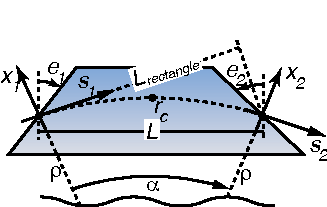
\includegraphics[width=1.05\textwidth]{rbend-coords.pdf}
    \caption{Rbend}
    \label{f:rbend}
  \end{subfigure}
  \begin{subfigure}[b]{0.32\textwidth}
    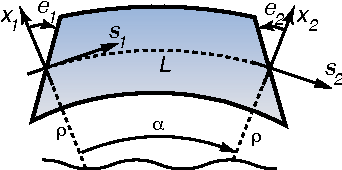
\includegraphics[width=1.05\textwidth]{sbend-coords.pdf}
    \caption{Sbend}
    \label{f:sbend}
  \end{subfigure}
  \begin{subfigure}[b]{0.32\textwidth}
    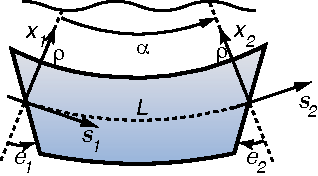
\includegraphics[width=1.05\textwidth]{sbend-rev.pdf}
    \caption{Reversed sbend}
    \label{f:sbend.rev}
  \end{subfigure}
  \hfill
  \caption[Coordinate systems for rbend and sbend elements.]
  { 
Coordinate systems for (a) normal (non-reversed)\vn{rbend}, (b) normal \vn{sbend}, and (c)
\vn{reversed sbend} elements. The bends are viewed from ``above'' (viewed from positive $y$).
Normal bends have \vn{g}, \vn{angle}, and \vn{rho} all positive. Reversed bends have \vn{g},
\vn{angle}, and \vn{rho} all negative. The face angles \vn{e1} and \vn{e2} are drawn for
\vn{reference_pt} set to \vn{none} or \vn{center}. For (a) and (b), as drawn, the \vn{e1} and \vn{e2} face
angles are both positive. For (c), as drawn, \vn{e1} and \vn{e2} are both negative. In all cases,
\vn{L} is positive. Notice that for reversed bends, the $x$-axis points towards the center of the
bend while for normal bends the $x$-axis points towards the outside.
  }
  \label{f:bend}
\end{figure}

  \begin{description}
  %
  \index{angle}
  \item[angle] \Newline
The total design bend angle. A positive \vn{angle} represents a
bend towards negative $x$ values (see \fig{f:local.coords}).
  %
  \index{b_field}\index{db_field}
  \item[B_field, dB_field] \Newline
The \vn{B_field} parameter is the design magnetic bending field which determines the reference orbit
and the placement of lattice elements downstream from the bend. The \vn{dB_field} parameter is
the difference between the actual (``total'') field and the design field. Thus:
\begin{example}
  Actual B-field = B_field + dB_field
\end{example}
See the discussion of \vn{g} and \vn{dg} below for more details.
  %
  \index{e1}\index{e2}
  \item[e1, e2] \Newline
The rotation angle of the entrance pole face is \vn{e1} and at the exit face it is \vn{e2}. Zero
\vn{e1} and \vn{e2} for an \vn{rbend} gives a rectangular magnet (\fig{f:rbend}). Zero \vn{e1} and
\vn{e2} for an \vn{sbend} gives a wedge shaped magnet (\fig{f:sbend}).  An \vn{sbend} with an
\vn{e1} = \vn{e2} = \vn{angle}/2 is equivalent to an \vn{rbend} with \vn{e1} = \vn{e2} = 0.  This
formula holds for both positive and negative angles. For \vn{rbend} elements, the above discussion
is true if \vn{fiducial_pt} is set to \vn{none} or \vn{center}. If \vn{fiducial_pt} is set to
\vn{entrance_end}, then the face angles are measured with respect to the entrace coordinates $(s_1
x_1)$.
If the \vn{fiducial_pt} is set to \vn{exit_end}, the face angles are measured with respect to
the exit coordinates $(s_2, x_2)$. Thus
\begin{example}
  e1(f_pt=none) = e1(f_pt=entrance_end) - angle/2 = e1(f_pt=exit_end) + angle/2
  e2(f_pt=none) = e2(f_pt=entrance_end) + angle/2 = e2(f_pt=exit_end) - angle/2
\end{example}

Note: The correspondence between \vn{e1} and \vn{e2} and the corresponding parameters used in the
SAD program \cite{b:sad} is:
\begin{example}
  e1(Bmad) =  e1(SAD) * angle + ae1(SAD)
  e2(Bmad) =  e2(SAD) * angle + ae2(SAD)
\end{example}
  %
  \index{exact_multipoles}
  \item[exact_multipoles] \Newline
The \vn{exact_multipoles} switch can be set to one of:
\begin{example}
  off                 ! Default
  vertically_pure    
  horizontally_pure  
\end{example}
This switch determines if the multipole fields, both magnetic and electric, and including the
\vn{k1} and \vn{k2} components, are corrected for the finite curvature of the reference orbit in a
bend. See \sref{s:field.exact} for a discussion of what \vn{vertically} pure versus
\vn{horizontally} pure means. Setting \vn{exact_multipoles} to \vn{vertically_pure} means that the
individual $a_n$ and $b_n$ multipole components are used with the vertically pure solutions
\begin{equation}
  \bfB = \sum_{n = 0}^\infty \left[ \frac{a_n}{n+1} \nabla \phi_n^r + \frac{b_n}{n+1} \nabla \phi_n^i \right], \qquad
  \bfE = \sum_{n = 0}^\infty \left[ \frac{a_{en}}{n+1} \nabla \phi_n^i + \frac{b_{en}}{n+1} \nabla \phi_n^r \right]
\end{equation}
and if \vn{exact_multipoles} is set to \vn{horizontally_pure} the horizontally pure solutions
$\psi_n^r$ and $\psi_n^i$ are used instead of the vertically pure solutions $\phi_n^r$ and
$\phi_n^i$.

To use exact multipoles with PTC based tracking (\sref{c:methods}), the PTC exact model
tracking must be turned on. That is, in the lattice file set:
\begin{example2}
  ptc_com[exact_model] = T
\end{example2}
With exact model tracking, PTC always assumes that multipole coefficient values correspond to
\vn{horizontally_pure}. In this case, \bmad will convert \vn{vertically_pure} to
\vn{horizontally_pure} as needed when passing multipole coefficients to PTC. Note that in
the case where PTC is doing exact model tracking (\sref{s:integ}) but the
\vn{exact_multipoles} switch is set to \vn{off}, PTC will still be treating the multipoles
as \vn{horizontally_pure} even though \bmad tracking will be treating them as straight
line multipoles. Note: If the bend has an associated electric field, PTC will always be
doing exact modeling.
  %
  \index{fint}\index{fintx}\index{hgapx}\index{hgapx}
  \item[fint, fintx, \Newline hgap, hgapx] \Newline
The field integrals for the entrance pole face is given by the product of the \vn{fint} and
\vn{hgap} parameters with \vn{hgap} being the half gap between poles at the entrance face
\begin{equation}
  F_{H1} \equiv F_{int} \, H_{gap} = \int_{pole} \! \! ds \, \frac{B_y(s) \, (B_{y0} - B_y(s))}
  {2 \, B_{y0}^2}
  \label{fsbbb}
\end{equation}
For the exit pole face there is a similar equation using \vn{fintx} and \vn{hgapx} which defines
$F_{H2}$. In the above equation $B_{y0}$ is the field in the interior of the dipole. The values of
\vn{fint}, \vn{fintx}, \vn{hgap}, and \vn{hgapx} are never used in isolation when tracking. Only
the values for $F_{H1}$ and $F_{H2}$ matter.

If \vn{fint} or \vn{fintx} is given without a value then a value of 0.5 is used. If \vn{fint} or
\vn{fintx} is not present, the default value of 0 is used. Note: \mad does not have the \vn{fintx}
and \vn{hgapx} attributes. \mad just assumes that the values are the same for the entrance and exit
faces. For compatibility with \mad, if \vn{fint} is given but \vn{fintx} is not, then \vn{fintx} is
set equal to \vn{fint}. Similarly, \vn{hgapx} will be set to \vn{hgap} if \vn{hgapx} is not
given. Note that this setting of \vn{fintx} or \vn{hgapx} using the value of \vn{fint} or \vn{hgap}
will only be done before lattice expansion (\sref{s:expand}).

Note: To have an effect, both \vn{fint} and \vn{hgap} (or \vn{fintx} and \vn{hgapx}) must be non-zero.

Note: The SAD program uses \vn{fb1+f1} for the entrance fringe and \vn{fb2+f1} for the exit
fringe. The correspondence between the two is
\begin{example2}
  \(F_{H1}\) = fint  * hgap  = (fb1 + f1) / 12
  \(F_{H2}\) = fintx * hgapx = (fb2 + f1) / 12
\end{example2}

\index{Enge function}
\vn{fint} and \vn{hgap} can be related to the Enge function which is sometimes used to model the
fringe field. The Enge function is of the form
\begin{equation}
  B_y(s) = \frac{B_{y0}}{1 + \exp[P(s)]}
\end{equation}
where
\begin{equation}
  P(s) = C_0 + C_1 \, s + C_2 \, s^2 + C_3 \, s^3 + \, \ldots
\end{equation}
The $C_0$ term simply shifts where the edge of the bend is. If all the $C_n$ are zero except for
$C_0$ and $C_1$ then
\begin{equation}
  C_1 = \frac{1}{2 \,H_{gap} \, F_{int}}
\end{equation}
  %
  \item[fiducial_pt] \Newline
The \vn{fiducial_pt} parameter sets a fiducial point which can be used to keep the shape of the bend
constant when, in a program, the parameters \vn{rho}, \vn{g}, \vn{b_field} or \vn{angle} are varied.
Varying these parameters typically happens when doing machine design. Using a fiducial point can be
helpful when designing a machine usin bend magnets that already exist.

The \vn{fiducial_pt} parameter
has four possible settings:
\begin{example}
  none          ! No fiducial point (default).
  entrance_end  ! The entrance point is the fiducial point.
  center        ! The center of the reference curve is the fiducial point.
  exit_end      ! The exit point is the fiducial point.
\end{example}
With \vn{fiducial_pt} set to \vn{none} (the default). The bend shape is not held constant. With the
other three settings, the bend shape will be help constant as discussed in \sref{s:bend.fiducial}.
With \vn{fiducial_pt} set to \vn{entrance_end}, the reference trajectory at the entrance end is held
fixed in both position and orientation with respect to the bend face and \vn{g}, \vn{l} and \vn{e2},
along with the other depdendent parameters, are adjusted to both give the desired change in what was
varied (which is one of \vn{rho}, \vn{g}, \vn{b_field} or \vn{angle}) and to keep the shape of the
bend unchanged. See \fig{f:bend.fid1}. Similarly, if \vn{fiducial_pt} is set to \vn{center}, the
center of the reference trajectory is held fixed in both position and orientation and if
\vn{fiducial_pt} is set to \vn{exit_end}, the exit point is held fixed in both position and
orientation.
  %
  \index{g}\index{rho}\index{dg}
  \item[g, dg, rho] \Newline
The design bending radius which determines the reference coordinate system is \vn{rho} (see
\sref{s:ref}). \vn{g} = \vn{1/rho} is the curvature function and is proportional to the design
dipole magnetic field. \vn{g} is related to the design magnetic field \vn{B_field} via
\begin{equation}
  \text{g} = \frac{q}{p_0} \, \text{B_field} 
  \label{gqpb}
\end{equation}
where $q$ is the charge of the reference particle and $p_0$ is the reference momentum. It is
important to keep in mind that changing \vn{g} will change the design orbit (\sref{s:coords.3}) and
hence will move all downstream lattice elements in space.

The parameter \vn{dg} is the difference between the actual and the design bending strengths. The
relationship between \vn{dg} and \vn{dB_field} is analogous to the relationship between \vn{g} and
\vn{B_field} in \Eq{gqpb}. The actual (``total'') field strength is given by the sum:
\begin{example}
  Actual g = g + dg
\end{example}
Changing \vn{dg} leaves the design orbit and the positions of all downstream lattice elements
unchanged but will vary a particle's orbit. One common mistake when designing lattices is to vary
\vn{g} and not \vn{dg} which results in downstream elements moving around. See \Sref{s:ex.chicane}
for an example.

Note: A positive \vn{g}, which will bend particles and the reference orbit in the $-x$ direction
represents a field of opposite sign as the field due a positive \vn{hkick}.
  %
  \index{h1}\index{h2}
  \item[h1, h2] \Newline
The attributes \vn{h1} and \vn{h2} are the curvature of the entrance and exit pole faces. They are
present for compatibility with MAD but are not yet implemented in terms of tracking and other
calculations.
  %
  \index{k1}\index{b1_gradient}
  \item[k1, b1_gradient] \Newline
The normalized and unnormalized (\sref{s:field.master}) quadrupole strength. See \Eqs{bbb} and \eq{kqlbp}.

  %
  \index{k2}\index{b2_gradient}
  \item[k2, b2_gradient] \Newline
The normalized and unnormalized (\sref{s:field.master}) sextupole strength. See \Eqs{bbb} and \eq{kqlbp}.
  %
  \index{l}\index{l_chord}\index{l_arc}\index{l_sagitta}\index{l_rectangle}
  \item[l, l_arc, l_chord, l_sagitta]  \Newline
For compatibility with MAD, for an \vn{rbend}, \vn{l} is the chord length and not the arc length as
it is for an \vn{sbend}.  After reading in a lattice, \bmad will internally convert all \vn{rbend}s
into \vn{sbend}s, and the \vn{l_chord} attribute of the created \vn{sbend} will be set to the input
\vn{l}. The \vn{l} of the the created \vn{sbend} will be set to the true path length (see
above). Alternatively for an \vn{rbend}, instead of setting \vn{l}, the \vn{l_arc} attribute can be
used to set the true arc length. 

For \vn{sbend} elements, \vn{l_chord} will be set to the calculated chord length. For both types of
bends, the \vn{l_sagitta} parameter will be set to the sagitta length (The sagitta is the distance
from the midpoint of the arc to the midpoint of the chord). \vn{l_sagitta} can be negative and will have
the same sign as the \vn{g} parameter.

The \vn{l_rectangle} parameter is the ``rectangular'' length. See the documentation on the \vn{fiducial_pt}
parameter above.
  %
  item[l_rectangle] \Newline
The ``rectangular length'' is the distance between the entrance and exit points along the $s$ axis
defined by the setting of \vn{fiducial_pt}. \fig{f:rbend} shows \vn{l_rectangle} for
\vn{fiducial_pt} set to \vn{entrance_end}. If \vn{fiducial_pt} is set to \vn{none} or \vn{center},
\vn{l_rectangle} is the same as the chord length. If \vn{fiducial_pt} is set to \vn{entrance_end}
or \vn{exit_end} the rectangular length will be $\rho \sin\alpha$.
  %
  \index{ref_tilt}
  \item[ref_tilt] \Newline
The \vn{ref_tilt} attribute rotates a bend about the longitudinal axis at the entrance face of the
bend. A bend with \vn{ref_tilt} of $\pi/2$ and positive \vn{g} bends the element in the $-y$
direction (``downward''). See \fig{f:tilt.bend}. It is important to understand that \vn{ref_tilt},
unlike the \vn{tilt} attribute of other elements, bends both the reference orbit along with the
physical element. Note that the MAD \vn{tilt} attribute for bends is equivalent to the \bmad
\vn{ref_tilt}. Bends in \bmad do not have a \vn{tilt} attribute.

Important! Do not use \vn{ref_tilt} when doing misalignment studies for a machine. Trying to misalign
a dipole by setting \vn{ref_tilt} will affect the positions of all downstream elements! Rather, use the
\vn{roll} parameter.
  \end{description}

%---------------

\index{l}
The difference between \vn{rbend} and \vn{sbend} elements is the way the \vn{l}, \vn{e1}, and
\vn{e2} attributes are interpreted.  To ease the bookkeeping burden, after reading in a lattice,
\bmad will internally convert all \vn{rbend}s into \vn{sbend}s.  This is done using the following
transformation on \vn{rbend}s:
\begin{example}
  l_chord(internal) = l(input)
  l(internal) = 2 * asin(l_chord * g / 2) / g
  e1(internal) = e1(input) + theta / 2
  e2(internal) = e2(input) + theta / 2
\end{example}

The attributes \vn{g}, \vn{angle}, and \vn{l} are mutually dependent. If any two are specified for
an element \bmad will calculate the appropriate value for the third.  After reading in a lattice,
\vn{angle} is considered the dependent variable so if \vn{l} or \vn{g} is veried, the value of
\vn{angle} will be set to \vn{g * l}. if \vn{theta} is varied, \vn{l} will be set accordingly.

Since internally all \vn{rbend}s are converted to \vn{sbend}s, if one wants to vary the \vn{g}
attribute of a bend and still keep the bend rectangular, an overlay (\sref{s:overlay}) can be
constructed to maintain the proper face angles.  For example:
\begin{example}
  l_ch = 0.54
  g_in = 1.52
  l_coef = asin(l_ch * g_in / 2) / g_in
  my_bend: rbend, l = l_ch, g = g_in
  my_overlay: overlay = \{my_bend, my_bend[e1]:l_coef, my_bend[e2]:l_coef\}, 
                var = \{g\}, g = g_in
\end{example}
Notice that \vn{l_coef} is just \vn{arc_length/2}.

In the local coordinate system (\sref{s:ref}), looking from ``above'' (bend viewed from positive
$y$), and with \vn{ref_tilt} = 0, a positive \vn{angle} represents a particle rotating clockwise. In
this case. \vn{g} will also be positive. For counterclockwise rotation, both \vn{angle} and \vn{g}
will be negative but the length \vn{l} is always positive. Also, looking from above, a positive
\vn{e1} represents a clockwise rotation of the entrance face and a positive \vn{e2} represents a
counterclockwise rotation of the exit face. This is true irregardless of the sign of \vn{angle} and
\vn{g}. Also it is always the case that the pole faces will be parallel when
\begin{example}
  e1 + e2 = angle
\end{example}

Example bend specification:
\begin{example}
  b03w: sbend, l = 0.6, k1 = 0.003, fint  ! gives fint = fintx = 0.5
\end{example}

\vn{ptc_field_geometry} determines what reference coordinates PTC uses within a bend for calculating
higher order fields. This only affects tracking if PTC is being used and if
\vn{ptc_com[exact_model]} is set to True (\sref{s:bmad.ptc.com}). Possible values for
\vn{ptc_field_geometry} are:
\begin{example}
  sector      ! Default
  straight
\end{example}
For \vn{sector} reference coordinates, the field coordinate reference frame is with respect to the
arc of the reference trajectory. For \vn{straight} coordinates the coordinate reference frame is
with respect to the chord line. For a bend where there are no other fields besides the basic dipole
field, tracking is essentially unaffected.\footnote
  {
There will be a small difference due to the fact that with a \vn{straight} geometry tracking uses a
coordinate system with the $z$-axis along the chord and with a \vn{sector} geometry an integration step
uses the curvilinear coordinate system with the $z$-axis along the arc of the bend. If the length
of an integration step is made small, this difference will go to zero.
  }
When there are quadrupole or higher order fields, the fields are centered about the reference frame
set by \vn{ptc_field_geometry}. Since \bmad based tracking does not implement \vn{straight} geometry
tracking, \bmad and PTC tracking will show marked differences when \vn{ptc_field_geometry} is set to
\vn{straight}.

\newpage

%-----------------------------------------------------------------
\section{Capillary}
\label{s:capillary}
\index{capillary|hyperbf}

A \vn{capillary} element is a glass tube that is used to focus x-ray
beams.

General \vn{capillary} attributes are:
\begin{center}
\tt
\begin{tabular}{llll} \toprule
  {\sl Attribute Class}      & Section          & {\sl Attribute Class}      & Section         \\ \midrule
  Aperture limits            & \ref{s:limit}    & Offsets, Pitches \& Tilt   & \ref{s:offset}  \\ 
  Capillary Wall             & \ref{s:wall}     & Reference energy           & \ref{s:energy}  \\
  Custom Attributes          & \ref{s:cust.att} & Tracking \& transfer map   & \ref{c:methods} \\ 
  Description strings        & \ref{s:alias}    &                            &                 \\
  \bottomrule
\end{tabular}
\end{center}
\toffset
See \sref{s:list.capillary} for a full list of element attributes along with a their units.

\index{critical_angle_factor|hyperbf}
Attributes specific to a \vn{capillary} element are:
\begin{example}
  critical_angle_factor = <Real>    ! Critical angle * Energy (rad * eV)
\end{example}

The critical angle above which photons striking the capillary surface are
refracted into the capillary material scales as 1/Energy. The
constant of critical angle * energy is given by the \vn{critical_angle_factor}.

The inside wall of a capillary is defined using the same syntax used
to define the chamber wall for other elements (\sref{s:wall}).

The length of the capillary is a dependent variable and is given by
the value of \vn{s} of the last wall cross-section
(\sref{s:wall.capillary}).

\newpage

%-----------------------------------------------------------------
\section{Collimators: Ecollimator and Rcollimator} 
\label{s:col}
\index{ecollimator|hyperbf}
\index{rcollimator|hyperbf}

An \vn{ecollimator} is a drift with elliptic collimation. An \vn{rcollimator} is a drift
with rectangular collimation.

Alternatively, for defining a collimator with an arbitrary shape, a \vn{mask} element
(\sref{s:mask}) may be used.

General \vn{ecollimator} and \vn{rcollimator} attributes are:
\begin{center}
\tt
\begin{tabular}{llll} \toprule
  {\sl Attribute Class}      & Section          & {\sl Attribute Class}      & Section          \\ \midrule
  Aperture limits            & \ref{s:limit}    & Offsets, Pitches \& Tilt   & \ref{s:offset}   \\
  Chamber wall               & \ref{s:wall}     & Overlapping Fields         & \ref{s:overlap}  \\
  Custom Attributes          & \ref{s:cust.att} & Reference energy           & \ref{s:energy}   \\
  Description strings        & \ref{s:alias}    & Superposition              & \ref{s:super}    \\
  Hkick \& Vkick             & \ref{s:kick}     & Symplectify                & \ref{s:symp}     \\
  Integration settings       & \ref{s:integ}    & Field Maps                 & \ref{s:fieldmap} \\
  Is_on                      & \ref{s:is.on}    & Tracking \& transfer map   & \ref{c:methods}  \\
  Length                     & \ref{s:l}        &                            &                  \\
  \bottomrule
\end{tabular}
\end{center}
\toffset

Attributes specific to a \vn{capillary} element are:
\begin{example}
  px_aperture_width2 = <real>  ! px aperture half width
  px_aperture_center = <real>  ! px aperture center
  py_aperture_width2 = <real>  ! py aperture half width
  py_aperture_center = <real>  ! py aperture center
  z_aperture_width2  = <real>  ! z aperture half width
  z_aperture_center  = <real>  ! z aperture center
  pz_aperture_width2 = <real>  ! pz aperture half width
  pz_aperture_center = <real>  ! pz aperture center
\end{example}

Note: Collimators are the exception to the rule that the aperture is independent of any \vn{tilt}s.
See \sref{s:limit} for more details. Additionally, the default setting of \vn{offset_moves_aperture}
is \vn{True} for collimators (\sref{s:offset.ap}).

Besides the standard aperture settings \ref{s:limit} that can be used to limit $x$ and $y$ phase
space coordinates, collimators can be used to limit the other four phase space coordinates as well.  For
\vn{rcollimator} elements, particles are collimated if \vn{px_aperture_width2} is greater than zero
and
\begin{example}
  px < px_aperture_center - px_aperture_width2  or
  px > px_aperture_center + px_aperture_width2
\end{example}
with similar equations for \vn{py}, \vn{z}, and \vn{pz}. For \vn{ecollimator} elements, if
\vn{px_aperture_width2} and \vn{py_aperture_width2} are both nonzero, particles are collimated if
\begin{example}
  ((px - px_aperture_center) / px_aperture_width2)^2 + 
        ((py - py_aperture_center) / py_aperture_width2)^2 < 1
\end{example}
If one or both of \vn{px_aperture_width2} or \vn{py_aperture_width2} are zero, the computation is the
same as for an \vn{rcollimator}. A similar situation occurs for \vn{z} and \vn{pz}. 

Example:
\begin{example}
  d21: ecollimator, l = 4.5, x_limit = 0.09, y_limit = 0.05, 
              px_aperture_width2 = 0.3, py_aperture_width = 0.1
\end{example}

\newpage

%-----------------------------------------------------------------
\section{Converter}
\label{s:converter}
\index{converter|hyperbf}

A \vn{converter} element represents a target (plate) onto which particles are slammed in order to generate
particles of a different type. For example, a tungsten plate which is bombarded with electrons to
generate positrons.

General \vn{custom} attributes are:
\begin{center}
\tt
\begin{tabular}{llll} \toprule
  {\sl Attribute Class}      & Section           & {\sl Attribute Class}      & Section         \\ \midrule
  Aperture limits            & \ref{s:limit}     & Is_on                      & \ref{s:is.on}   \\
  Chamber wall               & \ref{s:wall}      & Length                     & \ref{s:l}       \\
  Custom Attributes          & \ref{s:cust.att}  & Offsets, pitches \& tilt   & \ref{s:offset}  \\
  Description strings        & \ref{s:alias}     & Reference energy           & \ref{s:energy}  \\ 
  Integration settings       & \ref{s:integ}     & Superposition              & \ref{s:super}   \\
                             &                   & Tracking \& transfer map   & \ref{c:methods} \\ 
  \bottomrule
\end{tabular}
\end{center}

The attributes specific to an \vn{converter} are 
\begin{example}
  distribution    = <Struct>    ! Outgoing particle distribution.
  pc_out_min      = <Real>      ! Minimum outgoing particle momentum (eV).
  pc_out_max      = <Real>      ! Maximum outgoing particle momentum (eV).
  angle_out_max   = <Real>      ! Maximum outgoing angle.
  species_out     = <SpeciesID> ! Output species.
  p0c             = <Real>      ! Output ref momentum.
  E_tot           = <Real>      ! Output ref energy. Dependent var (\sref{s:depend}).
\end{example}

The species of the outgoing particles is specified by the \vn{species_out} parameter
(\sref{s:species.name}).

The converter must be the last element in a lattice branch (\sref{s:branch.def}) except for possible
\vn{fork}, \vn{photon_fork} or \vn{marker} elements. A \vn{fork} or \vn{photon_fork} element
(\sref{s:fork}) after the converter is used to connect to the line containing the elements that come
after the converter Example:
\begin{example}
  parameter[particle] = electron
  parameter[geometry] = open
  to_after: fork, to_line = after_cvter
  cvter, species_out = positron, p0c = 3e6, distribution = ...
  pre_linac: line = (..., cvter, to_after)
  after_cvter: line = (...)                ! Everything after the converter.
  after_cvter[beta_a] = 27; after_cvter[beta_b] = 32
  use, pre_linac
\end{example}
The line up to the fork element, \vn{pre_linac}, has the converter just before the \vn{fork}
element. The \vn{fork} element, called \vn{to_after}, connects to the line named \vn{after_cvter}
which contains all the elements after the converter. The reference particle and reference momentum
for the \vn{after_cvter} line is set to \vn{positron} and 3e6 respectively to agree with the setting
of \vn{species_out} and \vn{p0c} set in the converter element.

Since \bmad cannot calculate the appropriate Twiss and dispersion values after the converter, values
must be set in the lattice file.  Thus, in the above example, the starting beta function at the
beginning of the \vn{after_cvter} line is set to be $\beta_a = 27$~m and $\beta_b = 32$~m.

The \vn{p0c} and \vn{E_tot} attributes of the converter set the reference momentum or energy at the
exit end of the converter. At least one of these attributes must be set. If both are set, \vn{E_tot}
is calculated to be consistent with \vn{p0c}.

The \vn{distribution} parameter of a \vn{converter} element specifies the distribution of outgoing
particles for a given converter thickness. Multiple \vn{distribution} instances with differing
thicknesses may be present in an element. The actual thickness of the converter will be taken to be
the element's, length \vn{L} parameter. During tracking, the outgoing distribution will be computed
by interpolating between the two distributions that bracket the actual thickness. The exception is
when there is only one\vn{distribution} present. In this case, the calculation will just use that
distribution for the calculation independent of the element length. Example:
\begin{example}
cvter: converter, ..., distribution = \{
    material = tungsten,      ! Optional. Not used in tracking.
    thickness = 0.003,        ! Converter thickness for this distribution.
    sub_distribution = \{...\}, ! Distribution at one incoming momentum.
    sub_distribution = \{...\}, ! Distribution at another incoming momentum.
    ...                       ! etc.
  \}
\end{example}
The \vn{material} component is optional and is only for recording the converter material. Each
\vn{distribution} is made up of a number of \vn{sub_distribution} components. Each one specified the
outgoing distribution for a given incoming particle momentum. During tracking, interpolation is used
to compute the distribution appropriate for an incoming particle with a given momentum. It is an
error in the momentum of the incoming particle is outside the range of the momentums specified
in the \vn{sub_distributions}. A given \vn{sub_distribution} will look like:
\begin{example}
  sub_distribution = \{
    pc_in = 3e8,            ! Incoming momentum*c (eV)>
    prob_pc_r = \{...\},      ! Momentum and radius probability table 
    direction_out = \{...\},  ! Momentum orientation probability coefs
  \}
\end{example}

A \vn{sub_distribution} has three components: The \vn{pc_in} component specifies the incoming
particle momentum appropriate for the \vn{sub_distribution}, the \vn{prob_pc_r} component holds a
two-dimensional table of the probability $P(p_\txt{out}, r)$ (\Eq{nnprp}), and \vn{direction_out}
holds the coefficients for calculating the outgoing particle direction. \vn{prob_pc_r} look like:
\begin{example}
  prob_pc_r = \{
    r_values = [0.0, 4.9e-5, 1.25e-4, ...],
    row = \{pc_out = 1.55e6, prob = [0.0, 6.1e-6, 1.23e-5, ...]\}, 
    row = \{pc_out = 3.96e6, prob = [0.0, 1.1e-5, ...]\},
    ...                   ! More rows
  \}
\end{example}
A \vn{probl_pc_r} has one \vn{r_values} component and multiple \vn{row} components. The
\vn{r_values} component is a vector of radius values for the columns of the probability table.  The
value for the first column is always zero and the radius values are strictly increasing.  Each
\vn{row} component represents one row of the table. Each row has a momentum value \vn{pc_out} in eV
along with a \vn{prob} component which is a vector of probability values. The length of a \vn{prob}
vector is always equal to the length of the \vn{r_values} vector which is the number of columns in
the table. The probability value of the first column is always zero which reflects the fact that
there is vanishing area in an annulus of width $dr$ as $r$ tends to zero.

The \vn{direction_out} component of \vn{sub_distribution} look like:
\begin{example}
  direction_out = \{
    c_x = \{...\},
    alpha_x = \{...\},
    alpha_y = \{...\},
    beta = \{...\},
    dxds_min = \{...\},
    dxds_max = \{...\},
    dyds_max = \{...\}
  \}
\end{example}
The \vn{c_x}, \vn{alpha_x}, \vn{alpha_y}, and \vn{beta}, components of \vn{direction_out} give the
coefficients for calculating $c_x$, $\alpha_x$, $\alpha_y$, and $\beta$ respectively in
\Eq{pxsxs}. The other three components give, \vn{dxds_min}, \vn{dxds_max}, and \vn{dyds_max} give
the range for $x'$ and $y'$ over which \Eq{pxsxs} is valid. By symmetry, \vn{dyds_min} will be equal
to \vn{-dydx_max}. The form of all these components is similar. For example:
\begin{example}
  dxds_min = \{
    fit_1d_r = \{pc_out = 1.5e+06, poly = [-2.48, -658.4, -2.26e5, 1.71e+8]\},
    fit_1d_r = \{pc_out = 3.9e+06, poly = [...]\}, 
    ...,
    C = 2.99394,
    fit_2d_pc = \{k = 1.96e-8, poly = [1.0, -4.10e-10, 3.7e-16, 2.77e-27]\},
    fit_2d_r = \{k = 4.2e-4, poly = [-4.50, 400.2, -108985, 9.18e+06]\},
  \}
\end{example}
Here there are multiple \vn{fit_1d_r} components, one for each fit $\Gamma_i$ fit function
(\Eq{gcr}).  The \vn{pc_out} sub-component of a \vn{fit_1d_r} component gives the momentum $p_i$ at
which the fit function fits the data and the \vn{poly} sub-component of \vn{fit_1d_r} gives the
polynomial coefficients needed for \Eq{gcr}. The $C$, \vn{fit_2d_pc} and \vn{fit_2d_r} components
are used for computing $\Xi$ (\Eq{xkpkr}). The \vn{k} sub-components of \vn{fit_2d_pc} and
\vn{fit_2d_r} give $k_p$ and $k_r$ respectively in \Eq{xkpkr} and the \vn{poly} sub-components of
\vn{fit_2d_pc} and \vn{fit_2d_r} give the polynomial coefficients $w_n$ and $k_n$ respectively.

To calculate the distributions and output the appropriate \vn{distribution} structures which then
can be incorporated into a \bmad lattice, there is modeling code that is distributed with
\bmad. Specifically, it is in the directory
\begin{example}
  \$ACC_ROOT_DIR/util_programs/converter_element_modeling
\end{example}
[See your local \bmad Guru if you don't know how to find this directory.] There is documentation for
running the program in this directory. The distribution modeling is based upon the \vn{Geant}
simulation toolkit for the simulation of the passage of particles through matter.

The mechanics of how \bmad generates outgoing particles is discussed in \Sref{s:converter.track}.
In a tracking simulation, a single outgoing particle is generated for each incoming particle.  All
outgoing particles will be assigned a \vn{weight} that represent how many actual outgoing particles
a single actual incoming particle will generate. For example, if an actual incoming particle with a
particular momentum would generate, on average, 0.42 particles, the outgoing particle in the
simulation will have a weight of 0.42.  To make simulations more efficient, the \vn{pc_out_min},
\vn{pc_out_max}, and \vn{angle_out_max} parameters can be set to restrict the momentum and angle
range of outgoing particles. If the outgoing particles are restricted in momentum or angle, the
weight of the outgoing particles will be appropriately adjusted such that the weighted distribution
of outgoing particles within the momentum and/or angle restricted range is independent of the
whether or not there is are restrictions.  A value of zero (the default) for any one of these
parameters means that that parameter is ignored.

\newpage

%-----------------------------------------------------------------
\section{Crab_Cavity}
\label{s:crab}
\index{crab_cavity|hyperbf}

A \vn{crab_cavity} is an RF cavity that gives a $z$-dependent kick. This is useful in colliding beam
machines, where there is a finite crossing angle at the interaction point, to rotate the beams near the IP.

General \vn{crab_cavity} attributes are:
\begin{center}
\tt
\begin{tabular}{llll} \toprule
  {\sl Attribute Class}      & Section           & {\sl Attribute Class}      & Section            \\ \midrule
  Aperture limits            & \ref{s:limit}     & Length                     & \ref{s:l}          \\
  Chamber wall               & \ref{s:wall}      & Offsets, pitches \& tilt   & \ref{s:offset}     \\
  Custom Attributes          & \ref{s:cust.att}  & Reference energy           & \ref{s:energy}     \\ 
  Description strings        & \ref{s:alias}     & Superposition              & \ref{s:super}      \\
  Hkick \& Vkick             & \ref{s:kick}      & Symplectify                & \ref{s:symp}       \\
  Integration settings       & \ref{s:integ}     & Field Maps                 & \ref{s:fieldmap}   \\
  Is_on                      & \ref{s:is.on}     & Tracking \& transfer map   & \ref{c:methods}    \\
  \bottomrule
\end{tabular}
\end{center}
\toffset
See \sref{s:list.crab.cavity} for a full list of element attributes along with a their units.

The attributes specific to an \vn{crab_cavity} are 
\index{gradient}\index{phi0}\index{n_cell}
\index{phi0_multipass}\index{e_loss}
\index{rf_frequency}\index{voltage}\index{cavity_type}
\begin{example}
  gradient        = <Real>    ! Accelerating gradient (V/m).
  phi0            = <Real>    ! Phase (rad/2\(\pi\)) of the reference particle with 
                              !   respect to the RF. phi0 = 0 is on crest.
  phi0_multipass  = <Real>    ! Phase (rad/2\(\pi\)) with respect to a multipass lord (\sref{s:multipass}).
  rf_frequency    = <Real>    ! RF frequency (Hz).
  harmon          = <Real>    ! Harmonic number
  harmon_master   = <Logic>   ! Is harmon or rf_frequency the dependent var with ref energy changes?
  voltage                     ! Cavity voltage. Dependent attribute (\sref{s:depend}).
\end{example}

The Hamiltonian  $H_{\text{crab}}$ for a thin crab cavity is\cite{b:crab1}:
\begin{equation}
  H_{\text{crab}} = -r_q \, V\, x \, \sin(k \, t + 2 \, \pi \, \phi_0)
\end{equation}
where $x$ and $z$ are particle coordinates, $r_q$ is the charge relative to the reference
particle, $V$ is the ``effective'' cavity voltage, $\phi_0$ is a user settable
phase, and $k$ is the wave number
\begin{equation}
  k = \frac{2 \, \pi \, f_{\text{rf}}}{c}
\end{equation}
Which give kicks of
\begin{align} 
  \Delta p_x &= -\frac{1}{c \, P_0} \, \frac{\partial H_{\text{crab}}}{\partial x} = 
    \frac{r_q \, V}{c \, P_0} \, \sin(k \, t + 2 \, \pi \, \phi_0) \CRNO 
  \Delta E &= -\frac{\partial H_{\text{crab}}}{\partial t} = 
    r_q \, V \, \, k \, x \, \cos(k \, t + 2 \, \pi \, \phi_0) 
\end{align} 
Note: The sign of $H_{\text{crab}}$ used by Authors in the literature is not standardized. \bmad
uses the convention such that a particle with the charge of the reference particle and with $z$ and
$V$ positive will have a positive $\Delta p_x$.

In the above equations $r_q$ is the relative charge between the reference particle (set by the
\vn{parameter[particle]} parameter in a lattice file) and the particle being tracked through the
cavity. For example, if the reference particle and and the tracked particle are the same, $r_q$ is
unity independent of the type of particle tracked.

The equations of motion can also be derived from analysis of a TM110 cavity mode for particles near
the centerline\cite{b:kim}. With this mode, the transverse kick is due to the magnetic field and the
longitudinal kick is due to the electric field. Using this, the integrated electric and magnetic
fields needed for spin tracking are:
\begin{align}
  \int \! B_y &= \frac{-V}{c} \, \sin(k \, z + 2 \, \pi \, \phi_0) \CRNO 
  \int \! E_s &=  \beta \, V \, \, k \, x \, \cos(k \, z + 2 \, \pi \, \phi_0) 
\end{align}
where $\beta = v/c$ is the normalized speed of the particle.

\newpage

%-----------------------------------------------------------------
\section{Crystal}
\label{s:crystal}
\index{crystal|hyperbf}

\begin{figure}[tb]
  \centering
  \includegraphics[width=5in]{crystal-ele.pdf}
  \caption[Crystal element geometry.]
{Crystal element geometry.  A) Geometry for Bragg diffraction. The geometry shown is for
\vn{ref_tilt} = 0 (reference trajectory in the $x$-$z$ plane). The angle $\alpha_H$
(\vn{alpha_angle}) is the angle of the $\bfH$ vector with respect to the surface normal $\bfhat
n$. For $\psi$ (\vn{psi_angle}) zero, the incoming reference orbit, the outgoing reference orbit,
$\bfhat n$, and $\bfH$ are all coplanar. B) Geometry for Laue diffraction. In this case there are
three outgoing beams: The Bragg diffracted beam, the forward diffracted beam, and the undiffracted
beam.}
  \label{f:crystal}
\end{figure}

A \vn{crystal} element represents a crystal used for photon diffraction.

General \vn{crystal} attributes are:
\begin{center}
\tt
\begin{tabular}{llll} \toprule
  {\sl Attribute Class}      & Section          & {\sl Attribute Class}      & Section         \\ \midrule
  Aperture limits            & \ref{s:limit}    & Surface Properties         & \ref{s:surface} \\ 
  Custom Attributes          & \ref{s:cust.att} & Symplectify                & \ref{s:symp}    \\
  Description strings        & \ref{s:alias}    & Offsets, Pitches \& Tilt   & \ref{s:offset}  \\
  Reference energy           & \ref{s:energy}   & Tracking \& transfer map   & \ref{c:methods} \\
  Reflection tables          & \ref{s:reflect}  &                            &                 \\
  \bottomrule
\end{tabular}
\end{center}
\toffset
See \sref{s:list.crystal} for a full list of element attributes along with a their units.

\index{psi_angle}
\index{b_param}\index{bragg_angle}\index{crystal_type}
\index{follow_diffracted_beam}\index{thickness}
Attributes specific to a \vn{crystal} element are:
\begin{example}
  b_param            = <Real>       ! b parameter for photons with the reference energy.
  crystal_type       = <String>     ! Crystal material (\sref{s:cryst.list}) and reflection plane.
  psi_angle          = <Real>       ! Rotation of H-vector about the surface normal.
  thickness          = <Real>       ! Thickness of crystal for Laue diffraction.
  ref_orbit_follows  = <which_beam> ! Reference orbit aligned with what outgoing beam?
  graze_angle_in     = <Real>       ! Angle between incoming ref orbit and surface.
  graze_angle_out    = <Real>       ! Angle between outgoing ref orbit and surface.
\end{example}

%  is_mosaic          = <Logical>    ! Is a mosaic crystal? Default = False
%  mosaic_thickness   = <Real>       ! Mosaic element thickness
%  mosaic_angle_rms_in_plane  = <Real> ! In-plane mosaic angular half-width.
%  mosaic_angle_rms_out_plane = <Real> ! Out-of-plane angular half-width. 

\index{bragg_angle_in}\index{bragg_angle_out}\index{alpha_angle}
\index{tilt_corr}\index{d_spacing}\index{v_unitcell}\index{l}
\index{ref_wave_length}\index{dbragg_angle_de}
\index{pendellosung_period_sigma}\index{pendellosung_period_pi}
Dependent variables (\sref{s:depend}) specific to a \vn{crystal} element are:
\begin{example}
  alpha_angle                ! Angle of H-vector with respect to the surface normal.
  bragg_angle                ! Nominal Bragg angle at the reference wave length. 
  bragg_angle_in             ! Incoming grazing angle for Bragg diffraction.
  bragg_angle_out            ! Outgoing grazing angle for Bragg diffraction.
  d_spacing                  ! Lattice plane spacing. 
  darwin_width_pi            ! Darwin width for pi polarized light (radians).
  darwin_width_sigma         ! Darwin width for sigma polarized light (radians).
  dbragg_angle_de            ! Variation of the Bragg angle with energy (radians/eV).
  l                          ! Length of reference orbit.
  pendellosung_period_pi     ! Pendellosung period for pi polarized light.
  pendellosung_period_sigma  ! Pendellosung period for sigma polarized light.
  ref_wavelength             ! Reference wavelength (\sref{s:energy}). Dependent attribute (\sref{s:depend}).
  ref_cap_gamma              ! \(\Gamma\) at the reference wavelength.
  tilt_corr                  ! Tilt correction due to a finite psi_angle.
  v_unitcell                 ! Unit cell volume. 
\end{example}

The \vn{crystal_type} attribute defines the crystal material and diffraction lattice plane. The
syntax is \vn{"ZZZ(ijk)"} where \vn{ZZZ} is the material name and \vn{ijk} are the Miller indices
for the diffraction plane. For example,
\begin{example}
  b_cryst1: crystal, crystal_type = "Si(111)", b_param = -1, ...
\end{example}
The atomic formula is case sensitive so, for example, \vn{"SI(111)"} is not acceptable. The list of
known crystal materials is given in \sref{s:cryst.list}. Given the \vn{crystal_type}, the spacing
between lattice planes (\vn{d_spacing}), the unit cell volume (\vn{v_unitcell}), and the structure
factor\cite{b:batterman} values can be computed.

The \vn{b_param} is the standard $b$ asymmetry factor
\begin{equation}
  b = \frac{\sin(\alpha_H + \theta_B)}{\sin(\alpha_H - \theta_B)} 
  \label{batat}
\end{equation}
where $\theta_B$ is the Bragg angle (\vn{bragg_angle}) 
\begin{equation}
  \theta_B = \sin^{-1} \left( \frac{\lambda}{2 \, d} \right)
  \label{tsl2d}
\end{equation}
and $\alpha_H$ (\vn{alpha_angle}) is the angle of the reciprocal lattice $\bfH$ vector with respect
to the surface normal as shown in \fig{f:crystal}A.  If \vn{b_param} is set to -1 then there is
Bragg reflection and \vn{alpha_H} is zero. If \vn{b_param} is set to 1 then there is Laue
diffraction again with \vn{alpha_H} zero. With the orientation shown in \fig{f:crystal}A,
\vn{alpha_H} is positive.

%The \vn{thickness} parameter is used with Laue diffraction and mosaic crystals.

The \vn{ref_orbit_follows} parameter sets how the outgoing reference orbit is constructed. This is
only relevant with Laue diffraction.  The possible settings of this parameter are:
\begin{example}
  bragg_diffracted      ! Default
  forward_diffracted
  undiffracted
\end{example}
The geometry of this situation is shown in \fig{f:crystal}B. The reference orbit for the
\vn{undiffracted} beam is just a straight line extension of the incoming reference trajectory. This
trajectory is that trajectory that photons whose energy is far from the Bragg condition (that is,
far from the reference energy) will follow. The \vn{forward_diffracted} reference orbit is parallel
to the \vn{undiffracted} trajectory and is the trajectory of the forward diffracted photons whose
energy is the reference energy and whose incoming orbit is on the incoming reference trajectory.
Finally, the \vn{bragg_diffracted} reference orbit (the default) is the backward diffracted orbit.

Note: Changing the setting of \vn{ref_orbit_follows} will change the reference orbit downstream of
the crystal which, in turn, will change the placement all downstream elements.

The value of the element reference orbit length \vn{l} is calculated by \bmad. \vn{L} will be zero
for Bragg diffraction. For Laue diffraction, \vn{l} will depend upon the crystal \vn{thickness} and
the setting of \vn{ref_orbit_follows}.

If \vn{psi_angle} is zero, the incoming reference orbit, the outgoing reference orbit, $\bfhat n$
and $\bfH$ are all coplanar. A non-zero \vn{psi_angle} Rotates the $\bfH$ vector around the $+\bfhat
x$ axis of the \vn{Element Reference Frame} (See \fig{f:crystal}A).

To keep the outgoing reference trajectory independent of the value of \vn{psi_angle}, the crystal
will be automatically tilted by the appropriate ``tilt correction'' \vn{tilt_corr}. The calculation
of \vn{tilt_corr} is outlined in \sref{s:crystal.trans}. \vn{tilt_corr} will be zero if
\vn{psi_angle} is zero.

The reference trajectory for a Bragg \vn{crystal} is that of a zero length bend
(\sref{s:mirror.coords}) and hence the length (\vn{l}) parameter of a crystal is fixed at zero. If
the \vn{graze_angle_in} and \vn{graze_angle_out} angles are zero (the default), the orientation of
the reference trajectory with respect to the crystal surface is specified by the incoming Bragg
angle \vn{bragg_angle_in} ($\theta_{g,in}$) and outgoing Bragg angle \vn{bragg_angle_out}
($\theta_{g,out}$) as shown in \fig{f:crystal}A. These angles are computed from the photon reference
energy and the other crystal parameters such that a photon with the reference energy traveling along
the reference trajectory will be in the center of the Darwin curve (\sref{s:crystal.tracking}). It
is sometimes convenient to be able to specify the angles that the reference trajectory makes with
respect to the crystal independent of the Bragg angles. To do this, set \vn{graze_angle_in} and
\vn{graze_angle_out} to the desired angles.

Notice that due to refraction at the surface, the computed \vn{bragg_angle} from \Eq{tsl2d} will
deviate slightly from the average of \vn{bragg_angle_in} and \vn{bragg_angle_out}.

The reference trajectory in the global coordinate system (\sref{s:global}) is determined by the
value of the \vn{ref_tilt} parameter along with the value of \vn{bragg_angle_in} +
\vn{bragg_angle_out}. These bragg angles take into account refraction so that the reference
trajectory downstream of the crystal will be properly centered with respect to the reference
photon. A positive \vn{bragg_angle_in} + \vn{bragg_angle_out} bends the reference trajectory in the
same direction as a positive \vn{g} for a bend element. The

A \vn{crystal} may be offset and pitched (\ref{s:offset}). The incoming local reference coordinates
are used for these misalignments.

When a crystal is bent (\sref{s:surface}), the $\bfH$ vector is assumed follow the surface
curvature. That is, it is assumed that the lattice planes are curved by the bending.

Example:
\begin{example}
  crystal_ele: crystal, crystal_type = "Si(111)", b_param = -1
\end{example}

The \vn{darwin_width_sigma} and \vn{darwin_width_pi} parameters are the computed Darwin width, in
radians, for sigma and pi polarized light respectively. Here the Darwin width $d\theta_D$ is defined
as the width at the $\eta = \pm 1$ points (cf.~Batterman\cite{b:batterman} Eq (32))
\begin{equation}
  d\theta_D = \frac{2 \, \Gamma \, |P| \, \text{Re} \! \left( [F_H \, F_{\Hbar}]^{1/2} \right)}
                 {|b|^{1/2} \, \sin\theta_{tot}}
\end{equation}
where
\begin{example}
  \(\theta_{tot}\) = bragg_angle_in + bragg_angle_out 
\end{example}

The \vn{pendellosung_period_sigma} and \vn{pendellosung_period_pi} are the pendellosung periods for
Laue diffraction. If the crystal is set up for Bragg diffraction then the values for these
parameters will be set to zero.

The \vn{dbragg_angle_de} parameter is the variation in Bragg angle with respect to the photon energy
and is given by the formula
\begin{equation}
  \frac{d\theta_B}{dE} = -\frac{\lambda}{2 \, d \, E \, \cos( \theta_B )}
\end{equation}

See Section~\sref{s:rowland} for an example lattice that can be used to simulate a Rowland circle
spectrometer.

%%----------------
%\subsection{Mosaic Crystal}
%
%A mosaic crystal is an idealized model of an imperfect crystal imagined to consist of numerous
%small perfect crystals called crystallites that are randomly misoriented. Currently, mosaic crystals
%can only be used with Laue orientation. Mosaic crystals are parameterized by four element
%parameters:
%\begin{example}
%  is_mosaic          = <Logical>    ! Is a mosaic crystal? Default = False
%  mosaic_thickness   = <Real>       ! Mosaic element thickness
%  mosaic_angle_rms_in_plane  = <Real> ! In-plane angular half-width. 
%  mosaic_angle_rms_out_plane = <Real> ! Out-of-plane angular half-width. 
%\end{example}
%The \vn{is_mosaic} logical is used to toggle between mosaic and non-mosaic tracking. Tracking in a
%mosaic is detailed in Section~\sref{s:mosaic.track}. The angular spread of the orientation of the
%crystallites in the diffraction plane is given by \vn{mosaic_angle_rms_in_plane}. This
%corresponds to rotations around the $y$-axis in the element reference frame in \fig{f:crystal}B. The
%\vn{mosaic_angle_rms_out_plane} parameter gives the angular spread of the crystallites for 
%
%The thickness of the mosaic is given by the \vn{mosaic_thickness} parameter. For \vn{Laue}
%diffraction (\vn{b_param} > 0), the actual mosaic thickness $T_m$ used is adjusted so that there is
%an integer number of mosaic layers. That is
%\begin{equation}
%  T_m(\text{in simulation} = \frac{T}{\text{nint} (T/T_m)}
%\end{equation}
%where $T$ is the crystal thickness and \vn{nint} is the nearest integer function.

\newpage

%-----------------------------------------------------------------
\section{Custom}
\label{s:custom}
\index{custom|hyperbf}

A \vn{custom} element is an element whose properties are defined outside of the standard \bmad
subroutine library. That is, to use a custom element, some programmer must write the appropriate
custom routines which are then linked with the \bmad subroutines into a program. \bmad will call the
custom routines at the appropriate time to do tracking, transfer matrix calculations, etc. See the
programmer who wrote the custom routines for more details! See \sref{s:custom.ele} on how to write
custom routines.

General \vn{custom} attributes are:
\begin{center}
\tt
\begin{tabular}{llll} \toprule
  {\sl Attribute Class}      & Section           & {\sl Attribute Class}      & Section         \\ \midrule
  Aperture limits            & \ref{s:limit}     & Is_on                      & \ref{s:is.on}   \\
  Chamber wall               & \ref{s:wall}      & Length                     & \ref{s:l}       \\
  Custom Attributes          & \ref{s:cust.att}  & Offsets, pitches \& tilt   & \ref{s:offset}  \\
  Description strings        & \ref{s:alias}     & Reference energy           & \ref{s:energy}  \\ 
  Field Maps                 & \ref{s:fieldmap}  & Superposition              & \ref{s:super}   \\
  Fringe fields              & \ref{s:fringe}    & Symplectify                & \ref{s:symp}    \\
  Integration settings       & \ref{s:integ}     & Tracking \& transfer map   & \ref{c:methods} \\ 
  \bottomrule
\end{tabular}
\end{center}
\toffset
See \sref{s:list.custom} for a full list of element attributes along with a their units.

\index{tracking_method}\index{mat6_calc_method}\index{field_calc}
As an alternative to defining a custom element, standard elements can
be ``customized'' by setting one or more of the following attributes
to \vn{custom}:
\begin{example}
  tracking_method       \sref{s:tkm}
  mat6_calc_method      \sref{s:xfer}
  field_calc            \sref{s:integ}
  aperture_type         \sref{s:limit}
\end{example}

As with a custom element, setting one of these attributes to
\vn{custom} necessitates the use of custom code to implement the
corresponding calculation.

\index{delta_e_ref}
\index{val1,  ..., Val12}
Attributes specific to a \vn{custom} element are
\begin{example}
  val1, ..., val12 = <Real>  ! Custom values 
  delta_e_ref      = <Real>  ! Change in energy.
\end{example}

\vn{delta_e_ref} is the energy gain of the {\it reference} particle
between the starting edge of the element and the ending edge.

Example:
\begin{example}
  c1: custom, l = 3, val4 = 5.6, val12 = 0.9, descrip = "params.dat"
\end{example}
In this example the \vn{descrip} string is being used to specify a
file that contains parameters for the element.

\newpage

%-----------------------------------------------------------------
\section{Detector}
\label{s:detector}
\index{detector|hyperbf}

A \vn{detector} element is used to detect particles and X-rays.  A
\vn{detector} is modeled as a grid of pixels which detect particles and x-rays
impinging upon them.

General \vn{detector} element attributes are:
\begin{center}
\tt 
\begin{tabular}{llll} \toprule
  {\sl Attribute Class}      & Section           & {\sl Attribute Class}      & Section         \\ \midrule
  Aperture limits            & \ref{s:limit}     & Offsets, pitches \& tilt   & \ref{s:offset}  \\
  Chamber Wall               & \ref{s:wall}      & Reference energy           & \ref{s:energy}  \\
  Custom Attributes          & \ref{s:cust.att}  & Superposition              & \ref{s:super}   \\
  Description strings        & \ref{s:alias}     & Tracking \& transfer map   & \ref{c:methods} \\
  Detector Geometry          & \ref{s:surf.grid} &                            &                 \\
  \bottomrule
\end{tabular}
\end{center}
\toffset
See \sref{s:list.detector} for a full list of element attributes along with a their units.

Attributes specific to a \vn{detector} element are:
\begin{example}
  pixel         = \{...\}   ! Define detector pixel grid.
\end{example}

The detector pixels are are arranged in a rectangular grid. The general syntax for defining
a detector pixel grid is
\begin{example}
  pixel = \{
      ix_bounds = (<ix_min>, <ix_max>),  ! Min/max index bounds in x-direction
      iy_bounds = (<iy_min>, <iy_max>),  ! Min/max index bounds in y-direction
      r0 = (<x0>, <y0>),                 ! (x,y) coordinates at grid origin
      dr = (<dx>, <dy>)                  ! Spacing between grid points.
          \}
\end{example}
See \Sref{s:surf.grid} for an explanation of the various pixel parameters.

Example:
\begin{example}
  det: detector, pixels = 
          \{ix_bounds = (-4,5), iy_bounds = (-10,10), dr = (0.01, 0.01)\}
\end{example}
This example defines a detector with 1~cm x 1~cm pixels.

\index{aperture_type}
The \vn{aperture_type} (\sref{s:limit}) parameter of a \vn{detector} will default to \vn{auto} which
will set the aperture limits to define a rectangular aperture that just cover the area of the pixel
grid.

A curved detector can be constructed by setting the appropriate surface curvature parameters
(\sref{s:surface}). It is assumed that any curvature is only in one dimension ($x$ or $y$). This
allows a straight forward mapping of the rectangular pixel grid onto the curved surface.

\newpage

%-----------------------------------------------------------------
\section{Diffraction_Plate}
\label{s:diff.plate}
\index{diffraction_plate|hyperbf}

A \vn{diffraction_plate} element is a flat surface oriented, more or
less, transversely to a x-ray beam through which photon can travel. A
\vn{diffraction_plate} can be used, for example, to model a Fresnel
zone plate or Young's double slits. A \vn{diffraction_plate} element
is used in places where diffraction effects must be taken into
account. This is in contrast to setting an aperture attribute
(\sref{s:limit}) for other elements where diffraction effects are
ignored.

A \vn{diffraction_plate} element is similar to a \vn{mask}
(\sref{s:mask}) element except that with a \vn{mask} element coherent
effects are ignored. Additionally, a \vn{mask} element can be used
with charged particles while a \vn{diffraction_plate} cannot.

General \vn{diffraction_plate} element attributes are:
\begin{center}
\tt 
\begin{tabular}{llll} \toprule
  {\sl Attribute Class}      & Section          & {\sl Attribute Class}      & Section         \\ \midrule
  Aperture limits            & \ref{s:limit}    & Offsets, pitches \& tilt   & \ref{s:offset}   \\ 
  Custom Attributes          & \ref{s:cust.att} & Mask geometry              & \ref{s:wall}    \\
  Description strings        & \ref{s:alias}    & Reference energy           & \ref{s:energy}  \\
  Is_on                      & \ref{s:is.on}    & Tracking \& transfer map   & \ref{c:methods} \\
  \bottomrule
\end{tabular}
\end{center}
\toffset
See \sref{s:list.diffraction.plate} for a full list of element attributes along with a their units.

\index{mode}\index{field_scale_factor}
Attributes specific to a \vn{diffraction_plate} element are:
\begin{example}
  mode               = <Type>   ! Reflection or transmission
  field_scale_factor = <Real>   ! Factor to scale the photon field
  ref_wavelength                ! Reference wavelength (\sref{s:energy}). Dependent attribute (\sref{s:depend}).
\end{example}

The \vn{mode} switch sets whether X-rays are transmitted through the
\vn{diffraction_plate} or or reflected. Possible values for the
\vn{mode} switch are:
\begin{example}
  reflection
  transmission        ! Default
\end{example}

The geometry of the plate, that is, where the openings (in
transmission mode) or reflection regions are, is defined using the
``wall'' attribute. See (\sref{s:wall}) for more details.

In transmission mode, a \vn{diffraction_plate} is nominally orientated
transversely to the beam. Like all other elements, the
\vn{diffraction_plate} can be reoriented using the element's offsets,
pitches and tilt attributes (\sref{s:offset}).

\index{aperture_type}
The \vn{aperture_type} (\sref{s:limit}) parameter of a
\vn{diffraction_plate} will default to \vn{auto} which will set the
aperture limits to define a rectangular aperture that just cover the
clear area of the plate.

\index{field_scale_factor}
The \vn{field_scale_factor}, if set to a non-zero value (zero is the
default) will be used to scale the field of photons as they pass through
the \vn{diffraction_plate} element:
\begin{example}
  field -> field * field_scale_factor
\end{example}
Scaling is useful since the electric field of photons traveling through a
\vn{diffraction_plate} are renormalized (see \Eqs{eeo4p} and
\eq{eek4p}). This can lead to large variation of the photon field and
can, for example, make visual interpretation of plots of field verses
longitudinal position difficult to interpret. \vn{field_scale_factor}
can be used to keep the field more or less constant.

A \vn{diffraction_plate} that is ``turned off'' (\vn{is_on} attribute
set to False), does not diffract at all and transmits through all
the light incident on it.

Example:
\begin{example}
  fresnel: diffraction_plate, wall = \{...\}
\end{example}

\newpage

%-----------------------------------------------------------------
\section{Drift}
\label{s:drift}
\index{drift|hyperbf}

A \vn{drift} element is a space free and clear of any fields.

General \vn{drift} attributes are:
\begin{center}
\tt
\begin{tabular}{llll} \toprule
  {\sl Attribute Class}      & Section          & {\sl Attribute Class}      & Section         \\ \midrule
  Aperture limits            & \ref{s:limit}    & Offsets, pitches \& tilt   & \ref{s:offset}  \\
  Custom Attributes          & \ref{s:cust.att} & Reference energy           & \ref{s:energy}  \\ 
  Description strings        & \ref{s:alias}    & Symplectify                & \ref{s:symp}    \\ 
  Length                     & \ref{s:l}        & Tracking \& transfer map   & \ref{c:methods} \\ 
  \bottomrule
\end{tabular}
\end{center}
\toffset
See \sref{s:list.drift} for a full list of element attributes along with a their units.

Example:
\begin{example}
  d21: drift, l = 4.5
\end{example}

Note: If a chamber wall (\sref{s:wall}) is needed for a field free
space, use a \vn{pipe} element instead of a \vn{drift} [a wall for a
drift is not allowed due to the way drifts are treated with
superposition. That is, drifts ``disappear'' when superimposed
upon. (\sref{s:super})].

\newpage

%-----------------------------------------------------------------
\section{E_Gun}
\label{s:e.gun}
\index{e_gun|hyperbf}

An \vn{e_gun} element represents an electron gun and encompasses a region starting from the cathode
were the electrons are generated.  General \vn{e_gun} attributes are:
\begin{center}
\tt
\begin{tabular}{llll} \toprule
  {\sl Attribute Class}      & Section           & {\sl Attribute Class}      & Section           \\ \midrule
  Aperture limits            & \ref{s:limit}     & Length                     & \ref{s:l}         \\
  Chamber wall               & \ref{s:wall}      & Mag \& Elec multipoles     & \ref{s:multip}    \\
  Custom attributes          & \ref{s:cust.att}  & Offsets, pitches \& tilt   & \ref{s:offset}    \\ 
  Description strings        & \ref{s:alias}     & Overlapping Fields         & \ref{s:overlap}   \\
  Field autoscaling          & \ref{s:autoscale} & Reference energy           & \ref{s:energy}    \\ 
  Hkick \& Vkick             & \ref{s:kick}      & Symplectify                & \ref{s:symp}      \\
  Integration settings       & \ref{s:integ}     & Field Maps                 & \ref{s:fieldmap}  \\
  Is_on                      & \ref{s:is.on}     & Tracking \& transfer map   & \ref{c:methods}   \\ 
  \bottomrule
\end{tabular}
\end{center}
\toffset
See \sref{s:list.e.gun} for a full list of element attributes along with a their units.

The attributes specific to an \vn{e_gun} are 
\index{voltage}\index{voltage_err}
\index{gradient}\index{gradient_err}
\begin{example}
  gradient       = <Real>    ! Gradient.
  gradient_err   = <Real>    ! Gradient error.
  gradient_tot               ! Net gradient = gradient + gradient_err. Dependent param (\sref{s:depend}).
  phi0           = <Real>    ! Phase (rad/2\(\pi\)) of the reference particle with 
                             !   respect to the RF. phi0 = 0 is on crest.
  phi0_err       = <Real>    ! Phase error (rad/2\(\pi\))
  rf_frequency   = <Real>    ! Frequency of the RF field.
  voltage        = <Real>    ! Voltage. Dependent attribute (\sref{s:depend}). 
  voltage_err    = <Real>    ! Voltage error. Dependent attribute (\sref{s:depend}). 
  voltage_tot                ! Net voltage = voltage + voltage_err. Dependent param (\sref{s:depend}).
\end{example}

The \vn{voltage} is simply related to the \vn{gradient} via the element length \vn{l}:
\begin{example}
  voltage = gradient * l
\end{example}
If the \vn{voltage} is set to a non-zero value, the length \vn{l} must also be non-zero to keep the
gradient finite.  A particle with the charge as the reference particle will have a positive energy
gain if the \vn{voltage} and \vn{gradient} are positive and vice versa.

\index{phi0_autoscale}\vn{field_autoscale}
The \vn{voltage} and \vn{gradient} are scaled by \vn{field_autoscale} and, if there is a
finite \vn{rf_frequency}, the phase of the frequency is shifted by \vn{phi0_autoscale} as
discussed in Section~\sref{s:autoscale}. Autoscaling can be toggled on/off by using the
\vn{autoscale_phase} and \vn{autoscale_amplitude} toggles.

An \vn{e_gun} may either be DC if the \vn{rf_frequency} component is zero of AC if
not. For an AC \vn{e_gun}, the phase of the \vn{e_gun}, The phase $\phi_\REF$
is 
\begin{example} 
  \(\phi_\REF\) = phi0 + phi0_err + phi0_autoscale 
\end{example}

\index{marker}\index{null_ele}
Electrons generated at the cathode can have zero initial momentum and
this presents a special problem (\sref{s:energy}). As a result, the
use of \vn{e_gun} elements are restricted and they can only be used in
a ``linear'' (non-recirculating) lattice branch. Only one \vn{e_gun}
can be present in a lattice branch and, if it is present, it must be,
except for possibly \vn{marker} or \vn{null_ele} elements, the first
element in any branch.
 
Note: In order to be able to avoid problems with a zero reference momentum at the beginning of the
\vn{e_gun}, the reference momentum and energy associated with an \vn{e_gun} element
(\sref{s:ref.energy}) is calculated as outlined in Section~\sref{s:energy}. Additionally, the
reference momentum at the exit end of the \vn{e_gun}, that is \vn{p0c}, must be non-zero. Thus, for
example, if \vn{p0c} is zero at the start of the lattice, the \vn{e_gun} voltage must be non-zero.

Additionally, in order to be able to avoid problems with a zero reference momentum at the
beginning of the \vn{e_gun}, absolute time tracking (\sref{s:rf.time}) is always used in
an \vn{e_gun} element independent of the setting of \vn{bmad_com[absolute_time_tracking]}
(\sref{s:bmad.common}).

Note: The default \vn{tracking_method} (\sref{s:tkm}) setting for an
\vn{e_gun} is \vn{time_runge_kutta} and the default
\vn{mat6_calc_method} is \vn{tracking}.

In this example the field of an e_gun is given by a grid of field
values (\sref{s:grid.field}):
\begin{example}
  apex: e_gun, l = 0.23, field_calc = fieldmap, rf_frequency = 187e6, 
                grid_field = call::apex_gun_grid.bmad
\end{example}
with the file \vn{apex_gun_grid.bmad} being:
\begin{example}
  \{
    m = 0, harmonic = 1,
    master_scale = voltage,
    geometry = rotationally_symmetric_rz,
    r0 = (0, 0),
    dr = (0.001, 0.001),
    pt(0,0) = ( (0, 0), (0, 0), (1, 0),  (0, 0), (0, 0), (0, 0)),
    pt(0,1) = ( (0, 0), (0, 0), (0.99, 0),  (0, 0), (0, 0), (0, 0)),
    ... \}
\end{example}

\newpage

%-----------------------------------------------------------------
\section{ELseparator}
\label{s:elsep}
\index{elseparator|hyperbf}

An \vn{elseparator} is an electrostatic separator.

General \vn{elseparator} attributes are:
\begin{center}
\tt
\begin{tabular}{llll} \toprule
  {\sl Attribute Class}      & Section           & {\sl Attribute Class}      & Section          \\ \midrule
  Aperture limits            & \ref{s:limit}     & Mag \& Elec multipoles     & \ref{s:multip}   \\
  Chamber wall               & \ref{s:wall}      & Offsets, pitches \& tilt   & \ref{s:offset}   \\
  Custom Attributes          & \ref{s:cust.att}  & Overlapping Fields         & \ref{s:overlap}  \\
  Description strings        & \ref{s:alias}     & Reference energy           & \ref{s:energy}   \\ 
  Fringe Fields              & \ref{s:fringe}    & Superposition              & \ref{s:super}    \\
  Hkick \& Vkick             & \ref{s:kick}      & Symplectify                & \ref{s:symp}     \\
  Integration settings       & \ref{s:integ}     & Field Maps                 & \ref{s:fieldmap} \\  
  Is_on                      & \ref{s:is.on}     & Tracking \& transfer map   & \ref{c:methods}  \\ 
  Length                     & \ref{s:l}         &                            &                  \\
  \bottomrule
\end{tabular}
\end{center}
\toffset
See \sref{s:list.elseparator} for a full list of element attributes along with a their units.

\index{gap}
\index{e_field}
\index{voltage}
Attributes specific to an \vn{elseparator} element are:
\begin{example}
  gap = <Real> ! Distance between electrodes
  voltage      ! Voltage between electrodes. This is a settable dependent variable (\sref{s:depend}).
  e_field      ! Electric field. This is a settable dependent variable (\sref{s:depend}).
\end{example}

\index{hkick}
\index{vkick}
For an \vn{elseparator}, the kick for a positively charged particle, with the magnitude of
the charge that is the same as that of the reference particle (set by \vn{parameter[particle]}
\sref{s:param}), is determined by \vn{hkick} and \vn{vkick}. The kick for a negatively
charged particle is opposite this. The \vn{gap} for an \vn{Elseparator} is used to compute
the voltage for a given kick
\begin{example}
  e_field (V/m) = sqrt(hkick^2 + vkick^2) * P0 * c_light / L
  voltage (V) = e_field * gap
\end{example}
Specifying a \vn{e_field} or \vn{voltage} with no tilt results in a vertical kick.

Examples:
\begin{example}
  h_sep1: elsep, l = 4.5, hkick = 0.003, gap = 0.11
  h_sep2: elsep, l = 4.5, e_field = 1e5, tilt = pi/2
\end{example}

\newpage

%-----------------------------------------------------------------
\section{EM_Field}
\label{s:em.field}
\index{em_field|hyperbf}

An \vn{em_field} element can contain general electro-magnetic (EM)
fields. Both AC and DC fields are accommodated.  General \vn{em_field}
attributes are:
\begin{center}
\tt
\begin{tabular}{llll} \toprule
  {\sl Attribute Class}      & Section           & {\sl Attribute Class}      & Section         \\ \midrule
  Aperture limits            & \ref{s:limit}     & Is_on                      & \ref{s:is.on}   \\
  Chamber wall               & \ref{s:wall}      & Length                     & \ref{s:l}       \\ 
  Custom Attributes          & \ref{s:cust.att}  & Offsets, pitches \& tilt   & \ref{s:offset}  \\
  Description strings        & \ref{s:alias}     & Reference energy           & \ref{s:energy}  \\
  Field Maps                 & \ref{s:fieldmap}  & Superposition              & \ref{s:super}   \\
  Hkick \& Vkick             & \ref{s:kick}      & Symplectify                & \ref{s:symp}    \\
  Integration settings       & \ref{s:integ}     & Tracking \& transfer map   & \ref{c:methods} \\
  \bottomrule
\end{tabular}
\end{center}
\toffset
See \sref{s:list.em.field} for a full list of element attributes along with a their units.

\index{constant_ref_energy}
Attributes specific to an \vn{em_field} element are:
\begin{example}
  constant_ref_energy = <Logical> ! Is the reference energy constant? Default = True.
  polarity   = <Real>  ! For scaling the field.
\end{example}

The \vn{polarity} value is used to scale the magnetic field. By
default, \vn{polarity} has a value of 1.0.  Example:
\begin{example}
  wig1: wiggler, l = 1.6, polarity = -1, cartesian_map = \{...\}
\end{example}

If the \vn{constant_ref_energy} logical is set to \vn{True} (the default), the reference energy
(\sref{s:ref.energy}) at the exit end of the element is set equal to the entrance end reference
energy. This is the same behavior for most other elements. If the \vn{constant_ref_energy} logical
is set to \vn{False}, the reference energy at the exit end is calculated like it is in a
\vn{lcavity} or \vn{e_gun} element.

Note: \vn{em_field} elements will be created when elements are superimposed (\sref{s:super}) and
there is no other suitable element class.

\newpage

%-----------------------------------------------------------------
\section{Feedback}
\label{s:feedback}
\index{feedback|hyperbf}

A \vn{feedback} element is a lord element with two types of slaves called the \vn{input} slaves and
\vn{output} slaves.  The feedback element gathers information about particle trajectories from the
input slaves and uses this to either adjust beam trajectories in the output slaves and/or adjust
parameters in the output slaves. A feedback element could be used, for example, to simulate RF feedback
systems or beam position feedback, or cooling of a proton beam by a beam of electrons.

General \vn{feedback} element attributes are:
\begin{center}
\tt
\begin{tabular}{llll} \toprule
  {\sl Attribute Class}      & Section           & {\sl Attribute Class}      & Section         \\ \midrule
  Custom Attributes          & \ref{s:cust.att}  & Description strings        & \ref{s:alias}     \\
  \bottomrule
\end{tabular}
\end{center}
\toffset
See \sref{s:list.feedback} for a full list of element attributes along with a their units.

NOTE! 2024/3 The \vn{feedback} element is currently under development so changes can be expected in the future.

Attributes specific to a \vn{feedback} element are:
\begin{example}
  input_ele  = <list>   ! Lattice element(s) feedback element gets information from
  output_ele = <list>   ! Lattice elements(s) where the feedback element can influence
                        !   particle trajectories or element parameters.
\end{example}

The \vn{input_ele} parameter defines a list of lattice elements that specify, when tracking particles,
where the \vn{feedback} element will monitor particle trajectories. The \vn{output_ele} parameter
defines a list of lattice elements that specify the points at which the \vn{feedback} element can
either modify particle trajectories and/or modify lattice element parameters.

The \vn{<list>} of lattice elements uses the standard \bmad name matching conventions as given in
\sref{s:ele.match}. If commas are used in the \vn{<list>}, the list must be enclosed in curly
backets \vn{\{...\}} to avoid ambiguities. Curly brackets are optional when commas are not
used. Examples:
\begin{example}
  fff: feedback, input_ele = bpm5, 
                  output_ele = kicker3      ! Single input and output elements.
  fe2: feedback, input_ele = \{bpm5\}, 
                  output_ele = rfcavity::*  ! Output to all RF cavities.
  g7: feedback, input_ele = \{mon1, mon2\}, 
                  output_ele = type::IRQ    ! Match to element's type field.
\end{example}

The set of \vn{input_ele} and \vn{output_ele} elements will be \vn{minor_slave} slaves of the
\vn{control_lord} \vn{feedback} element. Like other lord elements (\vn{group}s, \vn{overlay}s,
etc.), particles are never tracked through a \vn{feedback} element itself.

Since feedback systems vary greatly in how they work, a generic feedback element is not currently
planned (but could be in the future as more experience is gained developing feedback simulation
code).  This being the case, a program must be specifically setup to handle feedback elements. In
particular, feedback elements in a lattice will not affect any calculation when using the \vn{Tao}
program (but \vn{Tao} can still be used to inspect feedback elements and their slaves).

Currently, the only program that handles \vn{feedback} elements is the \vn{e_cooling} program that
is located in the \vn{bsim} directory of a \vn{Bmad} Release (and this program is currently under
development and not ready for doing simulations). A feedback aware program will handle the task
of feedback related parameter setup so the program documentation should be consulted for specifics.

\newpage

%-----------------------------------------------------------------
\section{Fiducial}
\label{s:fiducial}
\index{fiducial|hyperbf}

A \vn{fiducial} element is used to fix the position and orientation of the reference orbit within
the global coordinate system at the location of the \vn{fiducial} element. A \vn{fiducial} element
will affect the global floor coordinates (\sref{s:global}) of elements both upstream and downstream
of the fiducial element.

Other elements that are used to shift the lattice in the global coordinate frame are
\vn{floor_shift} (\sref{s:floor.ele}) and \vn{patch} (\sref{s:patch}).

General \vn{fiducial} element attributes are:
\begin{center}
\tt
\begin{tabular}{llll} \toprule
  {\sl Attribute Class}      & Section           & {\sl Attribute Class}      & Section         \\ \midrule
  Aperture limits            & \ref{s:limit}     & Reference energy           & \ref{s:energy}  \\
  Custom Attributes          & \ref{s:cust.att}  & Superposition              & \ref{s:super}   \\
  Description strings        & \ref{s:alias}     & Tracking \& transfer map   & \ref{c:methods} \\ 
  \bottomrule
\end{tabular}
\end{center}
\toffset
See \sref{s:list.fiducial} for a full list of element attributes along with a their units.

\index{origin_ele}\index{origin_ele_ref_pt}
\index{x_origin}\index{y_origin}
\index{z_origin}\index{theta_origin}
\index{phi_origin}\index{psi_origin}
Attributes specific to a \vn{fiducial} elements are:
\begin{example}
  origin_ele        = <Name>     ! Reference element.
  origin_ele_ref_pt = <location> ! Reference pt on reference ele.
  dx_origin         = <Real>     ! x-position offset
  dy_origin         = <Real>     ! y-position offset
  dz_origin         = <Real>     ! z-position offset
  dtheta_origin     = <Real>     ! orientation angle offset.
  dphi_origin       = <Real>     ! orientation angle offset.
  dpsi_origin       = <Real>     ! orientation angle offset.
\end{example}

For tracking purposes, the \vn{fiducial} element is considered to be a
zero length marker. That is, the transfer map through a \vn{fiducial}
element is the unit map.

A \vn{fiducial} element sets the global floor coordinates (\sref{s:global}) of itself and of the
elements, both upstream and downstream, around it. This can be thought of as a two step process. The
first step is to determine the global coordinates of the \vn{fiducial} element itself, and the
second step is to shift the coordinates of the elements around it. That is, shifting the position
of a \vn{fiducial} element shifts the lattice elements around it as one solid body.

The floor coordinates of the \vn{fiducial} element are determined starting with an \vn{origin_ele}
element. If \vn{origin_ele} is not specified, the origin of the global coordinates (\sref{s:global}
is used. If the \vn{origin_ele} has a finite length, the reference point may be chosen using the
\vn{origin_ele_ref_pt} attribute which may be set to one of
\begin{example}
  entrance_end
  center         ! Default
  exit_end
\end{example}

Once the origin reference position is determined, the reference
position of the \vn{fiducial} element is calculated using the offset
attributes 
\begin{example}
  [dx_origin,  dy_origin,  dz_origin]
  [dtheta_origin,  dphi_origin,  dpsi_origin]
\end{example}
The transformation between origin and fiducial positions is given in
\sref{s:patch.coords}.

\index{flexible patch}\index{patch}
Once the position of the \vn{fiducial} element is calculated, all elements of the lattice branch the
\vn{fiducial} element is contained in, {\em both} the upstream and downstream elements, are shifted
so that everything is consistent. That is, the \vn{fiducial} element orients the entire lattice
branch. The exception here is that if there are \vn{flexible} \vn{patch} elements (\sref{s:patch})
in the lattice branch, the \vn{fiducial} element will only determine the positions up to the
\vn{flexible} \vn{patch} element.

Example: A lattice branch with elements 0 through 103 has a \vn{fiducial} element at position 34 and
a \vn{flexible} \vn{patch} at position 67. In this case the \vn{fiducial} element will determine the
reference orbit for elements 0 through 66.

Rules: 
  \begin{itemize}
  \item
If an \vn{origin_ele} is specified, the position of this element must to calculated before the
position of the \vn{fiducial} element is calculated (\sref{s:ref}). This means, the \vn{origin_ele}
must be in a prior lattice branch from the branch the \vn{fiducial} element is in or the
\vn{origin_ele} in the same branch as the \vn{fiducial} element but is positioned upstream from the
\vn{fiducial} element and there is a \vn{flexible} \vn{patch} in between the two elements.
  \item
If a \vn{fiducial} element affects the position of element 0 in the lattice branch (that is, there
are no flexible \vn{patch} elements in between), any positioning of element 0 via \vn{beginning} or
\vn{line parameter} statements (\sref{s:beginning}) are ignored.
  \item
\vn{Fiducial} elements must not over constrain the lattice geometry.  For example, two \vn{fiducial}
elements may not appear in the same lattice branch unless separated by a \vn{flexible} \vn{patch}.

Another example is that if there are no flexible \vn{patch} elements in the lattice, and if branch
\vn{A} has a \vn{branch} element connecting to branch \vn{B}, the geometry of branch \vn{A} will be
calculated first and the geometry of branch \vn{B} can then be calculated from the known coordinates
of the \vn{fork} element. If branch \vn{B} contains a \vn{fiducial} element then this is an error
since the coordinate calculation never backtracks to recalculate the coordinates of the elements of
a branch once the calculation has finished with that branch.
  \end{itemize}

Example:
\begin{example}
  f1: fiducial, origin_ele = mark1, x_offset = 0.04
\end{example}
See \sref{s:ex.collide} for an example where a fiducial element is
used to position the second ring in a dual ring colliding beam 
machine.

\newpage

%-----------------------------------------------------------------
\section{Floor_Shift}
\label{s:floor.ele}
\index{floor_shift|hyperbf}

A \vn{floor_shift} element shifts the reference orbit in the global coordinate system without
affecting particle tracking. That is, in terms of tracking, a \vn{floor_shift} element is equivalent
to a \vn{marker} (\sref{s:mark}) element. 

Also see \vn{patch} (\sref{s:patch}) and \vn{fiducial} (\sref{s:fiducial}) elements.

General \vn{floor_shift} element attributes are:
\begin{center}
\tt
\begin{tabular}{llll} \toprule
  {\sl Attribute Class}      & Section           & {\sl Attribute Class}      & Section         \\ \midrule
  Aperture limits            & \ref{s:limit}     & Reference energy           & \ref{s:energy}  \\
  Custom Attributes          & \ref{s:cust.att}  & Superposition              & \ref{s:super}   \\
  Description strings        & \ref{s:alias}     & Tracking \& transfer map   & \ref{c:methods} \\
  Length                     & \ref{s:l}         &                            &                 \\
  \bottomrule
\end{tabular}
\end{center}
\toffset
See \sref{s:list.floor.shift} for a full list of element attributes along with a their units.

\index{l}\index{x_offset}\index{y_offset}\index{z_offset}
\index{tilt}\index{x_pitch}\index{y_pitch}
\index{origin_ele}\index{origin_ele_ref_pt}
Attributes specific to a \vn{floor_shift} elements are:
\begin{example}
  l                 = <Real>     ! Length
  x_offset          = <Real>     ! x offset from origin point.
  y_offset          = <Real>     ! y offset from origin point.
  z_offset          = <Real>     ! z offset from origin point.
  x_pitch           = <Real>     ! rotation of the reference coords.
  y_pitch           = <Real>     ! rotation of the reference coords.
  tilt              = <Real>     ! rotation of the reference coords.
  origin_ele        = <Name>     ! Reference element.
  origin_ele_ref_pt = <location> ! Reference pt on the reference ele.
\end{example}

The \vn{floor_shift} element sets the reference orbit at the exit end of the \vn{floor_shift}
element as follows: Start with the reference orbit at the \vn{origin_ele} reference point (see
below). This coordinate system is shifted using the offset, pitch and tilt parameters of the
\vn{floor_shift} element. The shifted coordinate system is used as the coordinate system at the exit
end of the \vn{floor_shift} element. The reference position transformation through a
\vn{floor_shift} element is given in Section~\sref{s:patch.coords}. In this respect, the \vn{floor_shift}
element is similar to the \vn{fiducial} element. The difference being that the \vn{fiducial} element affects
the global floor coordinates of elements both upstream and downstream of the \vn{fiducial} element while a
\vn{floor_shift} element only affects the floor position of elements downstream from it.
 
Like a \vn{fiducial} element, the transfer map through a \vn{floor_shift} element will be the
unit map. That is, the phase space coordinates of a particle will not change when tracking through a
\vn{floor_shift} element. 

The \vn{l} attribute can be used to adjust the longitudinal $s$ position.

The \vn{floor_shift} element can be used, for example, to restore the
correct global geometry when a section of the lattice is represented by, say,
a \vn{taylor} type element.

If an \vn{origin_ele} is not specified, the default \vn{origin_ele} is the lattice element before
the \vn{floor_shift} element.  If an \vn{origin_ele} is specified, \bmad needs to be able to
calculate the position of this element before the position of the \vn{fiducial} element is
calculated. See the discussion of the \vn{origin_ele} for \vn{fiducial} elements
(\sref{s:fiducial}).  Notice that if the \vn{origin_ele} is specified, and is different from the
element upstream from the \vn{floor_shift} element, the coordinates at the exit end of the
\vn{floor_shift} element is independent of the coordinates of the upstream element.

If the \vn{origin_ele} has a finite length, the reference point may be chosen using the
\vn{origin_ele_ref_pt} attribute which may be set to one of
\begin{example}
  entrance_end
  center
  exit_end         ! Default
\end{example}


PTC does not have an analogous element for the \vn{Floor_shift} element. When converting to PTC, a
\vn{floor_shift} element will be treated as a \vn{marker} element.

Example: 
\begin{example}
  floor: floor_shift, z_offset = 3.2
\end{example}
This offsets the element after the \vn{floor_shift} 3.2 meters from the previous
element.

\newpage

%-----------------------------------------------------------------
\section{Foil}
\label{s:foil}
\index{foil|hyperbf}

\begin{figure}[tb]
  \centering
  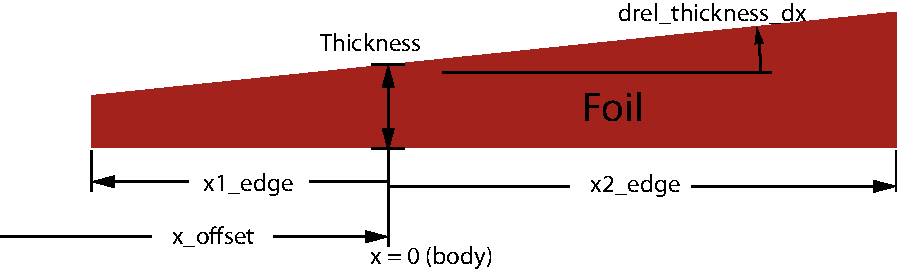
\includegraphics[width=5in]{foil.pdf}
  \caption[Foil geometry.]
{Foil geometry. Parameters \vn{thickness}, \vn{dthickness_dx}, \vn{x1_edge}, \vn{x2_edge},
\vn{y1_edge}, and \vn{y2_edge} determine the foil geometry in body coordinates (see \fig{f:coords}).
For the drawing, \vn{x1_edge} is negative (the associated edge is to the left of $x = 0$) and the
\vn{x2_edge} is positive.  Orientation parameters like \vn{x_offset} (\sref{s:offset}) orient the
foil with respect to laboratory coordinates but do not change the foil shape.}
  \label{f:foil}
\end{figure}

A \vn{foil} element represents a planar sheet of material which can strip electrons from a particle.
In conjunction, there will be scattering of the particle trajectory as well as an associated energy
loss.

General \vn{foil} attributes are:
\begin{center}
\tt
\begin{tabular}{llll} \toprule
  {\sl Attribute Class}      & Section           & {\sl Attribute Class}      & Section            \\ \midrule
  Aperture limits            & \ref{s:limit}     & Offsets, pitches \& tilt   & \ref{s:offset}     \\
  Custom Attributes          & \ref{s:cust.att}  & Reference energy           & \ref{s:energy}     \\ 
  Description strings        & \ref{s:alias}     & Superposition              & \ref{s:super}      \\
  Integration settings       & \ref{s:integ}     & Tracking \& transfer map   & \ref{c:methods}    \\ 
  Is_on                      & \ref{s:is.on}     &                            &                    \\
  \bottomrule
\end{tabular}
\end{center}
\toffset
See \sref{s:list.solenoid} for a full list of element attributes along with a their units.

Attributes specific to a \vn{foil} element are:
\begin{example}
  material_type       = <String>  ! Foil material.
  thickness           = <Real>    ! Material thickness (m).
  density             = <Real>    ! Input material density (kg/m^3).
  density_used                    ! Density value used in tracking (kg/m^3).
  radiation_length    = <Vector>  ! Input material radiation length (m).
  radiation_length_used           ! Radiation length used in tracking (m).
  area_density        = <Vector>  ! Input material area density (kg/m^2).
  area_density_used               ! Area density used in tracking (kg/m^2).
  F_factor            = <Real>    ! lynch_dahl scattering F factor. Default: 0.98.
  final_charge        = <Integer> ! Final charge state
  scatter_test        = <Logic>   ! For testing scattering. Default: False.
  scatter_method      = <Switch>  ! Scattering algorithm. Default: highland.
  dthickness_dx       = <Real>    ! Wedge slope when the foil is wedge shaped.
  x1_edge             = <Real>    ! Foil edge in the x-direction. Default: -99 m.
  x2_edge             = <Real>    ! Foil edge in the x-direction. Default:  99 m.
  y1_edge             = <Real>    ! Foil edge in the y-direction. Default: -99 m.
  y2_edge             = <Real>    ! Foil edge in the y-direction. Default:  99 m.
\end{example}

Scattering is simulated to be Gaussian distributed with a sigma calculated in one of two methods.
The two scattering algorithms are given in section~\sref{s:foil.scatter}. Which algorithm is used is
determined by the \vn{scatter_method} parameter which can be set to:
\begin{example}
  highland        ! Default
  lynch_dahl
  off             ! No scattering
\end{example}

Additionally, the \vn{scatter_test} logical may be used for testing. If set to True (default is
False), the random numbers used in \Eq{dpr1s} are set to 1.

Energy loss is calculated using the Bethe-Bloch formula as discussed in section~\sref{s:foil.eloss}.

The \vn{material_type} is the type of material which can be elemental or a compound material.

The radiation length used in the scattering calculation is given by the \vn{radiation_length_used}
parameter. For compound materials, this parameter is a vector with each value of the vector being the
radiation length of the corresponding component.  \vn{Radiation_length_used} cannot be set
directly. Rather, if the \vn{radiation_length} parameter is set non-zero, the value (or values for
a compound material) will be transferred to \vn{radiation_length_used}. If \vn{radiation_length} is
zero (the default), the value of \vn{radiation_length_used} will be set by \bmad using measured
values from the published literature.

Similarly, the \vn{area_density_used} (density of the material per unit of surface area) value (or
values for a compound material) needed for the calculation is not set directly but is set in one of
two ways depending upon if the material \vn{thickness} is non-zero or not. If \vn{thickness} is
non-zero, \vn{area_density_used} is set by the product of \vn{thickness} and \vn{density_used} while
the value of \vn{density_used} is set by \bmad to be either the value \vn{density} if the
\vn{density} is non-zero or by the measured density of the material as given in the published
literature. If \vn{thickness} is zero (the default), the value of \vn{area_density_used} is set
equal to the value of \vn{area_density}. Note that the value of \vn{density_used} is only used to
set \vn{area_density_used} when \vn{thickness} is non-zero and otherwise does not affect the
tracking calculation.

Example:
\begin{example}
  f1: foil, thickness = 1e-2, material_type = "B4C", 
          density = (2e3, 1e3), radiation_length = (5.49, 4.26)
\end{example}
Here, since \vn{material_type} is set to \vn{B4C}, there are two components: Boron and Carbon. If
\vn{density}, \vn{area_density}, or \vn{radiation_length} are present, they must have the same
number of values as material components. Values are set in order so, in the above example, the
Carbon component has a density of 1e3 and a radiation length of 4.26.\footnote
  {
From a computational standpoint it does not matter which parameter is associated with which component.
  }
In the case where there is a component material, either \vn{density} or \vn{area_density} needs to
be set since \bmad is not able to calculate appropriate values in this case. When there is only one
component, the parentheses may be omitted. Example:
Example:
\begin{example}
  stripper: foil, material_type = "Cu", thickness = 0.127, &
                                  radiation_length = 12.3, x1_edge = -0.3
\end{example}

In terms of element placement, The length of a \vn{foil} element (\Eq{l00l}) is considered to be
zero.  This is similar to the \vn{beambeam} element which is also considered to have zero length but
the interaction occurs over a finite length.

The 6x6 transfer matrix of a \vn{foil} element is the unit matrix. That is, scattering does
not affect the transfer matrix.

Particles going through the \vn{foil} are stripped to have a final charge given by
\vn{final_charge}.  The default is to fully strip the particle except if the particle has no
electrons to strip, there will be no change in charge state.

The foil has a rectangular shape and particles will only be considered to have hit the foil if:
\begin{example}
  x1_edge < x_particle < x2_edge  and
  y1_edge < y_particle < y2_edge
\end{example}
where (x_particle, y_particle) are the coordinates of the particle in the element body (not the
laboratory) coordinate system (\fig{f:coords}). See \fig{f:foil}. Particles that do not hit the
foil pass through the element without a change in charge nor a change in trajectory. The default
for \vn{x1_edge} and \vn{y1_edge} is -99~meters and for \vn{x2_edge} and \vn{y2_edge} the default is
+99~meters.

The \vn{dthickness_dx} parameter can be used to get a varying foil thickness. The thickness $t$ at
a point (in body coordinates) $(x,y)$ on the foil will be
\begin{equation}
  t = t_0 + x \, \frac{dt}{dx}
\end{equation}
where $t_0$ is the thickness given by the \vn{thickness} parameter and $dt/dx$ is given by the
\vn{dthickness_dx} parameter. To orient the wedge in the transverse plane, use the \vn{tilt}
orientation parameter (\sref{s:offset}). If \vn{dthickness_dx} is non-zero, the
\vn{area_density} and \vn{thickness} parameters are defined to be the area density and thickness at
$(x,y) = (0,0)$. If \vn{dthickness_dx} is non-zero, and if \vn{area_density} is
set (as opposed to setting the \vn{density}), then the \vn{thickness} must be non-zero since otherwise
the calculation of the area density at the point where a particle passes through the foil is singular.

If a \vn{foil} element is part of a lattice branch with a closed geometry, the closed orbit
calculation will tempararily set the \vn{scatter} parameter to false since scattering is a random
process and the closed orbit is not well defined in the presence of any random processes (similarly,
radiation fluctuations are also turned off for the closed orbit calculation).

\newpage

%-----------------------------------------------------------------
\section{Fork and Photon_Fork}
\label{s:fork}
\index{fork|hyperbf}
\index{photon_fork|hyperbf}

\begin{figure}[tb]
  \centering
  \includegraphics[width=5in]{x-fork.pdf}
  \caption[Example with photon_fork elements.]
  {
Example use of \vn{photon_fork} elements showing four X-ray lines (branches) attached to a machine.
  }
  \label{f:x.fork}
\end{figure}

A \vn{fork} or \vn{photon_fork} element marks the start of an alternative \vn{branch} for the beam
(or X-rays or other particles generated by the beam) to follow.

Collectively \vn{fork} and \vn{photon_fork} elements are called forking elements. An example
geometry is shown in \fig{f:x.fork}.  The \vn{branch} containing a forking element is called the
``\vn{base} \vn{branch}''. The \vn{branch} that the forking element points to is called the
``\vn{forked-to} \vn{branch}''.

The only difference between \vn{fork} and \vn{photon_fork} is that the default particle type for the
forked-to branch forked from a \vn{fork} element is the same particle type as the base branch. The
default particle type for the forked-to branch from a \vn{photon_fork} element is a photon. The actual
particle associated with a branch can be set by setting the \vn{particle} attribute of the forking
element.

General \vn{fork} and \vn{photon_fork} attributes are:
\begin{center}
\tt
\begin{tabular}{llll} \toprule
  {\sl Attribute Class}      & Section           & {\sl Attribute Class}      & Section         \\ \midrule
  Aperture limits            & \ref{s:limit}     & Length                     & \ref{s:l}       \\
  Chamber wall               & \ref{s:wall}      & Reference energy           & \ref{s:energy}  \\ 
  Custom Attributes          & \ref{s:cust.att}  & Superposition              & \ref{s:super}   \\
  Description strings        & \ref{s:alias}     & Tracking \& transfer map   & \ref{c:methods} \\ 
  Is_on                      & \ref{s:is.on}     &                            &                 \\
  \bottomrule
\end{tabular}
\end{center}
\toffset
See \sref{s:list.fork} for a full list of element attributes along with a their units.

Attributes specific to \vn{fork} and \vn{photon_fork} elements are:
\begin{example}
  direction    = <+/- 1>      ! Particles are entering or leaving?
  to_line      = <LineName>   ! What line to fork to.
  to_element   = <ElementID>  ! What element to attach to in the line being forked to.
  new_branch   = <T/F>        ! Make a new branch from the to_line? Default = True.
\end{example}

\index{patch}
Branch lines can themselves have forking elements. A branch line always starts out tangential to the
line it is branching from.  A \vn{patch} element (\sref{s:patch}) can be used to reorient the
reference orbit as needed. Example:
\begin{example}
  from_line: line = (... A, PB, B, ...)  ! Defines base branch
  pb: photon_fork, to_line = x_line
  x_line: line = (X_PATCH, X1, X2, ...)     ! Defines forked-to branch
  x_line[p0c] = 1e3                         ! Photon reference momentum   
  x_patch: patch, x_offset = 0.01
  use, from_line
\end{example}
In this example, a photon generated at the fork element \vn{PB} with $x = 0$ with respect to the
\vn{from_line} reference orbit through \vn{PB} will, when transferred to the \vn{x_line}, and
propagated through \vn{X_PATCH}, have an initial value for $x$ of $-0.01$.

Forking elements have zero length and, like \vn{marker} elements, the position of a particle tracked
through a forking element does not change.

Forking elements do not have orientational attributes like \vn{x_pitch} and \vn{tilt}
(\ref{s:offset}). If the orientation of the forked-to branch needs to be modified, this can be
accomplished using a \vn{patch} element at the beginning of the line.

\index{is_on}
The \vn{is_on} attribute, while provided for use by a program, is ignored by \bmad proper.

If the reference orbit needs to be shifted when forking from one ring to another ring, a patch can
be placed in a separate ``transfer'' line to isolate it from the branches defining the
rings. Example:
\begin{example}
  ring1: line = (... A, F1, B, ...)     ! First ring
  x_line: line = (X_F1, X_PATCH, X_F2)  ! "Transfer" line
  ring2: line = (... C, F2, D, ...)     ! Second ring
  use, ring1

  f1: fork, to_line = x_line
  f2: fork, to_line = x_line, direction = -1
  x_patch: patch, x_offset = ...
  x_f1: fork, to_line = ring1, to_element = f1, direction = -1
  x_f2: fork, to_line = ring2, to_element = f2
\end{example}
Here the \vn{fork} \vn{F1} in \vn{ring1} forks to \vn{x_line} which
in turn forks to \vn{ring2}.

The above example also illustrates how to connect machines for particles going in the reverse
direction. In this case, rather than using a single \vn{fork} element to connect lines, pairs of
\vn{fork} elements are used. \vn{Ring2} has a \vn{fork} element \vn{f2} that points back through
\vn{x_line} and then to \vn{ring1} via the \vn{x_f1} fork. Notice that both \vn{f2} and \vn{x_f2}
have their \vn{direction} attribute set to -1 to indicate that the fork is appropriate for particles
propagating in the -$s$ direction. Additionally, since \vn{f2} has \vn{direction} set to -1, it
will, by default, connect to the downstream end of the \vn{x_line}. The default setting of
\vn{direction} is 1.

It is important to note that the setting of \vn{direction} does not change the placement of elements
in the forked line. That is, the global position (\sref{s:global}) of any element is unaffected by
the setting of \vn{direction}. To shift the global position of a forked line, \vn{patch}
elements must be used. In fact, the \vn{direction} parameter is merely an indicator to a program on
how to treat particle propagation. The \vn{direction} parameter is not used in any calculation done
by \bmad.

\index{beginning_ele}\index{fiducial}\index{fork}\index{photon_fork}
\index{marker}\index{to_element}
The \vn{to_element} attribute for a forking element is used to designate the element of the forked-to
branch that the forking element connects to. To keep things conceptually simple, the \vn{to_element}
must be a ``marker-like'' element which has zero length and unit transfer matrix. Possible
\vn{to_element} types are:
\begin{example}
  beginning_ele
  fiducial
  fork and photon_fork
  marker
\end{example}
When the \vn{to_element} is not specified, the default is to connect to the beginning of the forked-to
branch if \vn{direction} is 1 and to connect to the end of the downstream branch if \vn{direction} is
-1. In this case, there is never a problem connecting to the beginning of the forked-to branch since
all branches have a \vn{beginning_ele} element at the beginning. When connecting to the end of the
forked-to branch the last element in the forked-to branch must be a marker-like element. Note that, by
default, a marker element is placed at the end of all branches (\sref{s:branch.construct})

The default reference particle type of a branch line will be a \vn{photon} is using a
\vn{photon_fork} or will be the same type of particle as the base branch if a \vn{fork} element is
used. If the reference particle of a branch line is different from the reference particle in the
base branch, the reference energy (or reference momentum) of a forked-to branch line needs to be set
using line parameter statements (\sref{s:beginning}). If the reference particle of a branch line is
the same as the reference particle in the base branch, the reference energy will default to the
reference energy of the base branch if the reference energy is not set for the branch.

Example showing an injection line branching to a ring which, in turn, branches to two x-ray lines:
\begin{example}
  inj: line = (..., br_ele, ...)            ! Define the injection line
  use, inj                                  ! Injection line is the root
  br_ele: fork, to_line = ring              ! Fork element to ring
  ring: line = (..., x_br, ..., x_br, ...)  ! Define the ring
  ring[E_tot] = 1.7e9                       ! Ring ref energy.
  x_br: photon_fork, to_line = x_line       ! Fork element to x-ray line
  x_line: line = (...)                      ! Define the x-ray line
  x_line[E_tot] = 1e3
\end{example}

The \vn{new_branch} attribute is, by default, \vn{True} which means that the lattice branch created
out of the \vn{to_line} line is distinct from other lattice branches of the same name. Thus, in the
above example, the two lattice branches made from the \vn{x_line} will be distinct. If
\vn{new_branch} is set to \vn{False}, a new lattice branch will not be created if a lattice branch
created from the same line already exists. This is useful, for example, when a chicane line branches
off from the main line and then branches back to it.

When a lattice is expanded (\sref{s:expand}), the branches defined by the \vn{use} statement
(\sref{s:use}) are searched for fork elements that branch to new forked-to branches. If found, the
appropriate branches are instantiated and the process repeated until there are no more branches to
be instantiated. This process does {\em not} go in reverse. That is, the lines defined in a lattice
file are not searched for fork elements that have forked-to instantiated branches. For example, if, in
the above example, the use statement was:
\begin{example}
  use, x_line
\end{example}
then only the \vn{x_line} would be instantiated and the lines \vn{inj} and \vn{ring} would be
ignored.

If the forked-to branch and base branch both have the same reference particle, and if the element
forked into is the beginning element, the reference energy and momentum of the forked-to branch will be
set to the reference energy and momentum at the fork element. In this case, neither the reference
energy nor reference momentum of the forked-to branch should be set. If it is desired to have the
reference energy/momentum of the forked-to branch different from what is inherited from the fork
element, a patch element (\sref{s:patch}) can be used at the beginning of the forked-to branch. In all
other cases, where either the two branches have different reference particles or the fork connects
to something other than the beginning element, there is no energy/momentum inheritance and either
the reference energy or reference momentum of the forked-to branch must be set.

How to analyze a lattice with multiple branches can be somewhat complex and will vary from program
to program. For example, some programs will simply ignore everything except the root branch. Hopefully
any program documentation will clarify the matter.

\newpage

%-----------------------------------------------------------------
\section{Girder}
\label{s:girder}
\index{girder|hyperbf}

\begin{figure}[t]
  \centering
  \includegraphics{girder.pdf}
  \caption[Girder example.] {
Girder supporting three elements labeled \vn{A}, \vn{B}, and \vn{C}.  $\calO_A$ is the reference
frame at the upstream end of element \vn{A} (\sref{s:ref.construct}), $\calO_C$ is the reference
frame at the downstream end of element \vn{C}, and $\calO_G$ is the default \vn{origin} reference
frame of the girder if the \vn{origin_ele} parameter is not set. $\bfr_{CA}$ is the vector from
$\calO_A$ to $\calO_C$. The length \vn{l} of the girder is set to be the difference in $s$ between
points $\calO_C$ and $\calO_A$.
  }
  \label{f:girder}
\end{figure}

A \vn{girder} is a support structure that orients the elements that are attached to it in space. A
girder can be used to simulate any rigid support structure and there are no restrictions on how the
lattice elements that are supported are oriented with respect to one another.  Thus, for example,
optical tables can be simulated.

General \vn{girder} attributes are:
\begin{center}
\tt
\begin{tabular}{llll} \toprule
  {\sl Attribute Class}      & Section           & {\sl Attribute Class}      & Section         \\ \midrule
  Custom Attributes          & \ref{s:cust.att}  & Length                     & \ref{s:l}       \\
  Description strings        & \ref{s:alias}     & Offsets, pitches \& tilt   & \ref{s:offset}  \\ 
  Is_on                      & \ref{s:is.on}     &                            &                 \\
  \bottomrule
\end{tabular}
\end{center}
\toffset
See \sref{s:list.girder} for a full list of element attributes along with a their units.

Attributes specific to a \vn{girder} are:
\index{origin_ele}\index{origin_ele_ref_pt}
\index{x_origin}\index{y_origin}
\index{z_origin}\index{theta_origin}
\index{phi_origin}\index{psi_origin}
Attributes specific to \vn{girder} elements are:
\begin{example}
  girder = \{<List>\}   ! List of elements on the Girder
  origin_ele        = <Name>     ! Reference element.
  origin_ele_ref_pt = <location> ! Reference pt on reference ele.
  dx_origin         = <Real>     ! x-position offset
  dy_origin         = <Real>     ! y-position offset
  dz_origin         = <Real>     ! z-position offset
  dtheta_origin     = <Real>     ! orientation angle offset.
  dphi_origin       = <Real>     ! orientation angle offset.
  dpsi_origin       = <Real>     ! orientation angle offset.
  l                 ! Girder "Length" (\ref{s:l}). Dependent attribute (\sref{s:depend}).
\end{example}

A simple example of a girder is shown in \fig{f:girder}. Here a girder supports three
elements labeled \vn{A}, \vn{B}, and \vn{C} where \vn{B} is a bend so the geometry is
nonlinear. Such a girder may specified in the lattice file like:
\begin{example}
  g1: girder = \{A, B, C\}
\end{example}

The \vn{girder} statement can take one of two forms:
\begin{example}
  <element_name>: GIRDER = \{<ele1>, <ele2>, ..., <eleN>\}, ... 
\end{example}
or
\begin{example}
  <element_name>: GIRDER = \{<ele_start>:<ele_end>\}, ... 
\end{example}

With the first form, a \vn{girder} element will be created for each section of the lattice where
there is a ``consecutive'' sequence of ``slave'' elements \vn{<ele1>} through \vn{<eleN>}.  This
section of the lattice from \vn{<ele1>} through \vn{<eleN>} is called the ``girder support region''.
``Consecutive'' here means there are no other elements in the girder support region except for
possibly \vn{drift} and/or \vn{marker} elements. \vn{Drift} elements cannot be controlled by a
girder\footnote{This policy was created to avoid the problem where the superposition of marker
elements on top of drifts would prevent girder formation.} but may appear in the girder slave
list. If a \vn{drift} does appear in the slave list, \vn{drift} elements will not be ignored when
determining if elements are consecutive. Note: If a drift-like element is desired to be supported by
a \vn{girder}, use a \vn{pipe} element instead. \vn{Marker} elements present in a girder support
region, but not mentioned in the girder slave list, are simply ignored.

The second form of a \vn{girder} statement specifies the first and last elements in the sequence of
elements to be supported. Everything in between except \vn{drift} elements will be supported by the
\vn{girder}.

Wild card characters (\sref{s:lat.attribs}) can be used in any element name in the girder slave
list. Additionally, beam line names (\sref{s:lines.wo.arg}) can be used. In this case, any
\vn{drift} elements within a beam line will be ignored.

A lattice element may have at most one \vn{girder} supporting it. However, a \vn{girder} can be
supported by another \vn{girder} which in turn can be supported by a third \vn{girder}, etc. Girders
that support other girders must be defined in the lattice file after the supported girders are
defined. Example:
\begin{example}
  g1: girder = \{A, B, C\}
  g2: girder = \{g1\}      ! g2 must come after g1!
\end{example}

A \vn{girder} may not directly support \vn{multipass_slave} (\sref{s:multipass}) or \vn{super_slave}
(\sref{s:super}) elements. Rather, a \vn{girder} may support the corresponding lord elements.

The reference frame from which the girder's offset, pitch, and tilt attributes (\sref{s:offset}) are
measured is constructed as follows: A reference frame, called the ``\vn{origin}'' reference frame
may be defined using the attributes \vn{origin_ele} and \vn{origin_ele_ref_pt} which constructs the
girder's \vn{origin} frame to be coincident with the reference frame of another element. Example:
\begin{example}
  g2: girder = \{...\}, origin_ele = Q, origin_ele_ref_pt = entrance_end
\end{example}
In this example, girder \vn{g2} has an \vn{origin} reference frame coincident with the entrance end
frame of an element named \vn{Q}. Valid values for \vn{origin_ele_ref_pt} are
\begin{example}
  entrance_end
  center        ! Default
  exit_end
\end{example}
For \vn{crystal}, \vn{mirror}, and \vn{multilayer_mirror} elements, setting \vn{origin_ele_ref_pt}
to \vn{center} results in the reference frame being the frame of the surface (cf.~\fig{f:surface}).

To specify that the global coordinates (\sref{s:global}) are to be used for a girder set
\vn{origin_ele} to
\begin{example}
  global_coordinates
\end{example}
Typically this is the same as using the \vn{beginning}
element (\sref{s:begin.ele}) as the \vn{origin_ele} except when the \vn{beginning} element is offset
or reoriented (\sref{s:beginning}).

If \vn{origin_ele} is not given, the default \vn{origin} frame is used. The default \vn{origin}
frame is constructed as follows: Let $\calO_A$ be the reference frame of the upstream end of the
first element in the list of supported elements. In this example it is the upstream end of element
\vn{A} as shown in the figure. Let $\calO_C$ be the downstream end of the last element in the list
of supported elements. In this example this is the downstream end of element \vn{C}. The origin of
the \vn{girder}'s reference frame, marked $\calO_G$ in the figure, will be half way along the vector
$r_{CA}$ from the origin of $\calO_A$ to the origin of $\calO_B$. The orientation of $\calO_G$ is
constructed by rotating the $\calO_A$ coordinates about an axis perpendicular to the $z$-axis of
$\calO_A$ and $\bfr_{CA}$ such that the $z$-axis of $\calO_G$ is parallel with $r_{CA}$.

Once the \vn{origin} reference frame is established, the reference frame of the girder can be offset
from the \vn{origin} frame using the parameters
\begin{example}
  dx_origin    dtheta_origin
  dy_origin    dphi_origin
  dz_origin    dpsi_origin
\end{example} 
The orientation of the \vn{girder}'s reference frame from the \vn{origin}
frame is given in \sref{s:patch.coords}. Example:
\begin{example}
  g3: girder = \{ ... \}, dx_origin = 0.03
\end{example}
This offsets girder \vn{g3}'s reference frame 3~cm horizontally from
the default \vn{origin} frame. If no offsets are given, the
\vn{origin} frame is the same as the girder's reference frame.

The length \vn{l} of a girder, which is not used in any calculations,
is a dependent attribute computed by \bmad and set equal to the $s$
path length between points $\calO_C$ and $\calO_A$.

\index{x_offset}\index{y_offset}\index{x_pitch}\index{y_pitch}\index{tilt}
The physical orientation of the girder with respect to it's reference
frame is, like other elements, determined by the offset, pitch and
tilt orientation attributes as outlined in \sref{s:offset} and
\sref{s:patch.coords}.  When a girder is shifted in space, the elements
it supports are also shifted.  In this case, the orientation
attributes (\vn{x_offset}, \vn{y_pitch}, etc.) give the orientation of
the element with respect to the \vn{girder}. The orientation with
respect to the local reference coordinates is given by
\vn{x_offset_tot}, which are computed from the orientation attributes
of the element and the \vn{girder}. An example will make this clear:
\begin{example}
  q1: quad, l = 2
  q2: quad, l = 4, x_offset = 0.02, x_pitch = 0.01
  d: drift, l = 8
  g4: girder = \{q1, q2\}, x_pitch = 0.002, x_offset = 0.03
  this_line: line = (q1, d, q2)
  use, this_line
\end{example}
\index{overlay}
In this example, \vn{g4} supports quadrupoles \vn{q1} and \vn{q2}.
Since the supported elements are colinear, the computation is greatly
simplified. The reference frame of \vn{g4}, which is the default
\vn{origin} frame, is at $s = 7$~meters which is half way between the
start of \vn{q1} at at $s = 0$~meters and the end of \vn{q2}) which is
at $s = 14$. The reference frames of \vn{q1} and \vn{q2} are at their
centers so the $s$ positions of the reference frames is
\begin{example}
  Element        S_ref   dS_from_g4
  q1             1.0     -6.0
  g4             7.0      0.0
  q2            12.0      5.0
\end{example}
Using a small angle approximation to simplify the calculation, the \vn{x_pitch} of \vn{g4} produces
an offset at the center of \vn{q2} of $0.01 = 0.002 * 5$. This, added to the offsets of \vn{g4} and
\vn{q2}, give the total \vn{x_offset}, denoted \vn{x_offset_tot} of \vn{q2} is $0.06 = 0.01 + 0.03 +
0.02$. The total \vn{x_pitch}, denoted \vn{x_pitch_tot}, of \vn{q2} is $0.022 = 0.02 + 0.001$.

A \vn{girder} that has its \vn{is_on} attribute set to False is considered to be unsifted with
respect to it's reference frame.

\newpage

%-----------------------------------------------------------------------------
\section{GKicker}
\label{s:gkicker}
\index{gkicker|hyperbf}

A \vn{gkicker} element is a ``general'' zero length kicker element that can displace
a particle in all six phase space dimensions.

General \vn{group} attributes are:
\begin{center}
\tt
\begin{tabular}{llll} \toprule
  {\sl Attribute Class}      & Section           & {\sl Attribute Class}      & Section         \\ \midrule
  Custom Attributes          & \ref{s:cust.att}  & Description strings        & \ref{s:alias}   \\ 
  \bottomrule
\end{tabular}
\end{center}
\toffset
See \sref{s:list.group} for a full list of element attributes along with a their units.

Attributes specific to a \vn{gkicker} are:
\index{x_kick}\index{px_kick}\index{y_kick}\index{py_kick}\index{z_kick}\index{pz_kick}
\begin{example}
  x_kick        = <Real>  ! X-position kick
  px_kick       = <Real>  ! X-momentum kick
  y_kick        = <Real>  ! Y-position kick
  py_kick       = <Real>  ! Y-momentum kick
  z_kick        = <Real>  ! Z-position kick
  pz_kick       = <Real>  ! Momentum kick
\end{example}

Example:
\begin{example}
  gk: gkicker, x_kick = 0.003, pz_kick = 0.12
\end{example}

\newpage

%-----------------------------------------------------------------------------
\section{Group}
\label{s:group}
\index{group|hyperbf}

\vn{Group} elements are a type of \vn{control} element (\sref{s:lord.slave}) used to make variations
in the attributes of other elements (called ``slave'' attributes) during execution of a program. For
example, to simulate the action of a control room knob that changes the beam tune in a storage ring,
a \vn{group} element can be used to vary the strength of selected quads in a specified manner. Also
see \vn{overlay} (\sref{s:overlay}) The difference between \vn{group} and \vn{overlay} elements is
that \vn{overlay} elements set the values of the attributes directly while \vn{group} elements make
delta changes to attribute values.

General \vn{group} attributes are:
\begin{center}
\tt
\begin{tabular}{llll} \toprule
  {\sl Attribute Class}      & Section           & {\sl Attribute Class}      & Section         \\ \midrule
  Custom Attributes          & \ref{s:cust.att}  & Is_on                      & \ref{s:is.on}   \\ 
  Description strings        & \ref{s:alias}     &                            &                 \\ 
  \bottomrule
\end{tabular}
\end{center}
\toffset
See \sref{s:list.group} for a full list of element attributes along with a their units.

There are two types of \vn{group} elements: \vn{Expression} based and \vn{knot} based.
The general syntax for a \vn{expression} based \vn{group} element is
\begin{example}
  name: GROUP = \{ele1[attrib1]:exp1, ele2[attrib2]:exp2, ...\}, 
              VAR = \{var1, var2, ...\}, var1 = init_val1, old_var1 = init_val_old1, ...
\end{example}
where \vn{ele1}[\vn{attrib1}], \vn{ele2}[\vn{attrib2}], etc. specify the slave attributes and
\vn{exp1}, \vn{exp2}, etc. are the arithmetical expressions, that are functions of \vn{var1},
\vn{var2}, etc., and are used to determine a value for the slave attributes.

The general syntax for a \vn{knot} based  \vn{group} element is
\begin{example}
  name: GROUP = \{ele1[attrib1]:\{y_knot_points1\}, ele2[attrib2]:\{y_knot_points2\}, ...\}, 
              VAR = \{var1\}, X_KNOT = \{x_knot_points\}, INTERPOLATION = \{type\}, 
              var1 = init_val1, old_var1 = init_val_old1, ...
\end{example}
When using knot points, the \vn{group} may only have one variable parameter.

\textbf{See Section~\sref{s:go.syntax} for a detailed description of this syntax.}

Example of a \vn{expression} based \vn{group} element:
\begin{example}
  gr1: group = \{q[k1]:a+b^2\}, var = \{a, b\}, a = 1, old_a = 2
  gr1[old_b] = 2
\end{example}
There are two numbers associated with each variable in a group: One number is the value of the
variable (also called the ``present'' value) and the other number is the ``old'' value. To refer to
these old values prepend the string ``old_'' to the variable name. Thus, in the above example, the
old variable values have names \vn{old_a} and \vn{old_b} and these old values can be set in the same
manner as the present values.

Example of a \vn{knot} based \vn{group} element:
\begin{example}
  gr2: group = \{beginning[E_tot]]:\{4e6,...\}\}, 
      var = \{time\}, x_knot = \{...\}, interpolate = cubic
\end{example}
Here the function used to translate from the \vn{group}'s variables to the slave attribute values is
a cubic spline interpolation based upon the knot points specified (\sref{s:go.syntax}).

A \vn{group} element is like an \vn{overlay} element in that a \vn{group} element controls the
attribute values of other ``slave'' elements. The difference is that the value of a slave attribute
that is controlled by (one or more) \vn{overlay} elements is uniquely determined by the controlling
\vn{overlay} elements. A \vn{group} element, on the other hand, is used to make changes in
value. An example will make this clear:
\begin{example}
  gr: group = \{q1[k1]:0.1*a^2\}, var = \{a\}, a = 2, old_a = 1
  q, quad, k1 = 0.5
\end{example}
When a program reads the lattice file, initially the value of \vn{q[k1]} will be 0.5 as set
in the definition of \vn{q}. Later, during lattice expansion (\sref{s:expand}), the group elements
are added to the lattice. When the group element \vn{gr} is added, the fact that \vn{old_a} and
\vn{a} are different causes the value of \vn{q[k1]} to be modified. The delta value is
\begin{example}
  delta = 0.1*a^2 - 0.1*old_a^2
        = 0.3
\end{example}
And this is added to the existing value of 0.5 so that the value of \vn{q[k1]} becomes 0.8.  After
the value of \vn{q[k1]} has been updated, the value of \vn{old_a} is automatically update to be the
present value of \vn{a} so that the value of \vn{q[k1]} will not be further modified.

In general, deltas used to modify slave attributes are computed as the difference between the
arithmetic expression evaluated with the present variable values and the arithmetic expression
evaluated with the old variable values.

Notice that in a lattice file the value of a slave attribute after the lattice is read in is
independent of whether the group is defined before or after elements whose attributes are controlled
by the group. This is true since the effect of a \vn{group} element happens when the lattice is
expanded, not when parser reads the \vn{group} definition. On the other hand, after the lattice has
been read in, if a program varies both a group variable and a slave attribute, the value of the
slave attribute will be dependent upon the order of which is modified first. For example, consider a
lattice containing:
\begin{example}
  gr: group = \{q[k1]:a^2\}, var = \{a\} 
  q, quad
\end{example}
Now if a program first sets \vn{gr[a]} to 0.3 and then sets \vn{q[k1]} to 0.5, the result is that
\vn{q[k1]} will have a value of 0.5. That is, the value of \vn{q[k1]} will be independent of
\vn{gr[a]}. If the setting is reversed so that \vn{q[k1]} is set first, the value of \vn{q[k1]} will
be 0.59. Since the result is order dependent, trying to ``simultaneously'' vary the attributes of
both group variables and slave attributes can lead to unpredictable results. For example, consider
lattice ``optimization'' where a program varies a set of lattice parameters to achieve certain goals
(for example, minimum beta at some point in the lattice, etc.). If the list of parameters to be
varied contains both group variables and slave attributes, the actual changes to slave attributes
may be different from what the user expects when the program varies its list of parameters.

During running of a program, If a \vn{group} element has been turned off (\vn{is_on} parameter set
false), a change to a variable of the group element is saved but the old variable value is not
updated and slave parameters are not affected. Subsequently, turning on the group element will
result in the appropriate changes to the slave parameters and the old variable value.

\index{overlay}\index{girder}
Different \vn{group} elements may control the same slave attribute and a \vn{group} element may
control other \vn{group}, \vn{overlay} or \vn{girder} element attributes. However, It does not make
sense, and it is not permitted, for a \vn{group} element to control the same attribute as an
\vn{overlay} element or for a \vn{group} element to control a \vn{dependent} attribute
(\sref{s:depend}). To setup a group element to control the same slave attribute as an \vn{overlay},
define an intermediate \vn{overlay}. For example:
\begin{example}
  ov: overlay = \{q{k1}\, q2[k1], ...\}, var = \{a\}
  q, quad                                          
  gr: group = \{ov_q[k1]:a^2\}, var = \{a\}  ! New
  ov_q: overlay = \{q\}, var = \{k1\}        ! New
\end{example}
In this example, the overlay \vn{ov} controls the attribute \vn{q[k1]} so it is not permitted for
\vn{q[k1]} to be a slave of a group element.  To have group control of \vn{q[k1]}, two elements are
introduced: the group \vn{gr} is setup controlling \vn{ov_q[k1]} and overlay \vn{ov_q} is an overlay
that controls \vn{q[k1]}. Notice that trying to control \vn{ov} directly by a group element will not
work since \vn{ov} controls multiple elements.

\index{accordion_edge}\index{start_edge}
\index{end_edge}\index{symmetric_edge}
\index{z_offset}
A \vn{group} can be used to control an elements position and length
using one of the following attributes:
\begin{example}
  accordion_edge  ! Element grows or shrinks symmetrically
  start_edge      ! Varies element's upstream edge s-position
  end_edge        ! Varies element's downstream edge s-position
  s_position      ! Varies element's overall s-position. Constant length.
\end{example}
With \vn{accordion_edge}, \vn{start_edge}, \vn{end_edge}, and \vn{symmetric_edge} the longitudinal
position of an elements edges are varied. This is done by appropriate control of the element's
length and the lengths of the elements to either side. In all cases the total length of the lattice
is kept invariant.

As an example, consider \vn{accordion_edge} which varies the edges of an element so that the center
of the element is fixed but the length varies:
\begin{example}
  gr: group = \{Z[accordion_edge]:1\}, var = \{offset\}
\end{example}
A change of, say, 0.1 \vn{gr}'s \vn{offset} variable moves both edges of element \vn{Z} by 0.1
meters so that the length of \vn{Z} changes by 0.2 meters but the center of \vn{Z} is constant. To
keep the total lattice length invariant, the lengths of the elements to either side are decreased by
0.1 meters to keep the total lattice length constant.
\begin{example}
  q10: quad, l = ...
  q11: quad, l = ...
  d1: drift, l = ...
  d2: drift, l = ...
  this_line: line = (... d1, q10, d2, q11, ...)
  gr2: group = \{q10[start_edge]:1\}, var = \{a\}, a = 0.1
\end{example}
The effect of  \vn{gr2[a]} will be to lengthen the length of
\vn{q10} and shorten the length of \vn{d1}.

A lattice file may contain lines and lattice elements that are not part of the actual finished
lattice when the lattice is constructed. \vn{Group} elements where {\em none} of its slave elements
are part of the finished lattice are ignored and are also not part of the finished lattice.  When a
\vn{group} element has some slave elements that are part of the finished lattice and some slave
elements that are not, the \vn{group} element as implemented in the finished lattice will only
control slave elements that actually exist in the finished. In any case, a slave element that a
\vn{group} element references must be defined (but not necessarily be used in the finished lattice)
in the lattice file. This rule is enforced in order to catch spelling mistakes.

If the arithmetical expression used for an \vn{group} contains an element attribute, care must be
taken if that element attribute is changed. This is discussed in \sref{s:arith} and
\sref{s:go.syntax}.

\newpage

%-----------------------------------------------------------------
\section{Hybrid}
\label{s:hybrid}
\index{hybrid|hyperbf}

A \vn{hybrid} element is an element that is formed by a program by concatenating other element
together. \vn{Hybrid} elements are used to reduce the number of elements in a lattice to speed up a
simulation. In terms of tracking a \vn{hybrid} element is essentially the same as a \vn{taylor}
element.

\newpage

%-----------------------------------------------------------------
\section{Instrument, Monitor, and Pipe}
\label{s:monitor}
\index{instrument|hyperbf}
\index{monitor|hyperbf}
\index{pipe|hyperbf}

Essentially \bmad treats \vn{instrument}, \vn{monitor}, and \vn{pipe} elements like a
\vn{drift}. There is a difference, however, when superimposing elements (\sref{s:super}). For
example, a \vn{quadrupole} superimposed on top of a \vn{drift} results in a free \vn{quadrupole}
element in the tracking part of the lattice and no lord elements are created. On the other hand, a
\vn{quadrupole} superimposed on top of a \vn{monitor} results in a \vn{quadrupole} element in the
tracking part of the lattice and this \vn{quadrupole} element will have two lords: A \vn{quadrupole}
superposition lord and a \vn{monitor} superposition lord. The exception is if a \vn{instrument},
\vn{monitor}, and \vn{pipe} is superimposed with an element with non-constant reference energy like
a \vn{lcavity}. In this case no \vn{instrument}, \vn{monitor}, or \vn{pipe} \vn{super_lord} element
is made.

General \vn{instrument}, \vn{monitor}, and \vn{pipe} attributes are:
\begin{center}
\tt
\begin{tabular}{llll} \toprule
  {\sl Attribute Class}      & Section             & {\sl Attribute Class}      & Section         \\ \midrule
  Aperture limits            & \ref{s:limit}       & Is_on                      & \ref{s:is.on}   \\
  Chamber wall               & \ref{s:wall}        & Length                     & \ref{s:l}       \\
  Custom Attributes          & \ref{s:cust.att}    & Offsets, pitches \& tilt   & \ref{s:offset}  \\ 
  Description strings        & \ref{s:alias}       & Reference energy           & \ref{s:energy}  \\
  Hkick \& Vkick             & \ref{s:kick}        & Superposition              & \ref{s:super}   \\
  Instrumental variables     & \ref{s:meas.attrib} & Symplectify                & \ref{s:symp}    \\
  Integration settings       & \ref{s:integ}       & Tracking \& transfer map   & \ref{c:methods} \\
  \bottomrule
\end{tabular}
\end{center}
\toffset
See \sref{s:list.instrument} for a full list of element attributes along with a their units.

\index{x_offset}
\index{y_offset}
\index{x_pitch}
\index{y_pitch}
\index{tilt}
The \vn{offset}, \vn{pitch}, and \vn{tilt} attributes are not
used by any \bmad routines. If these attributes are used by a program
they are typically used to simulate such things as measurement
offsets. The \vn{is_on} attribute is also not used by \bmad
proper. Example:
\begin{example}
  d21: instrum, l = 4.5
\end{example}

\newpage

%-----------------------------------------------------------------
\section{Kickers: Hkicker and Vkicker}
\label{s:hvkicker}
\index{hkicker|hyperbf}
\index{vkicker|hyperbf}

An \vn{hkicker} gives a beam a horizontal kick and a \vn{vkicker} gives a 
beam a vertical kick. Also see the \vn{kicker} (\sref{s:kicker}) element.

General \vn{hkicker} \vn{vkicker} attributes are:
\begin{center}
\tt
\begin{tabular}{llll} \toprule
  {\sl Attribute Class}      & Section           & {\sl Attribute Class}      & Section         \\ \midrule
  Aperture limits            & \ref{s:limit}     & Is_on                      & \ref{s:is.on}   \\
  Chamber wall               & \ref{s:wall}      & Length                     & \ref{s:l}       \\
  Custom Attributes          & \ref{s:cust.att}  & Mag \& Elec multipoles     & \ref{s:multip}  \\
  Description strings        & \ref{s:alias}     & Offsets, pitches \& tilt   & \ref{s:offset}  \\
  Field Maps                 & \ref{s:fieldmap}  & Reference energy           & \ref{s:energy}  \\ 
  Fringe Fields              & \ref{s:fringe}    & Superposition              & \ref{s:super}   \\
  Hkick \& Vkick             & \ref{s:kick}      & Symplectify                & \ref{s:symp}    \\
  Integration settings       & \ref{s:integ}     & Tracking \& transfer map   & \ref{c:methods} \\
  \bottomrule
\end{tabular}
\end{center}
\toffset
See \sref{s:list.hvkicker} for a full list of element attributes along with a their units.

\index{kick}
\index{hkick}
\index{vkick}
Note that \vn{hkicker} and \vn{vkicker} elements use the
\vn{kick} attribute while a \vn{kicker} uses the \vn{hkick} and \vn{vkick} 
attributes. Example:
\begin{example}
  h_kick: hkicker, l = 4.5, kick = 0.003
\end{example}

\newpage

%-----------------------------------------------------------------
\section{Kicker}
\label{s:kicker}
\index{kicker|hyperbf}

\index{hkick}\index{vkick}
\index{h_displace}\index{v_displace}
A \vn{kicker} can deflect a beam in both planes. Note that a \vn{kicker} uses the \vn{hkick} and
\vn{vkick} attributes while \vn{hkicker} and \vn{vkicker} elements use the \vn{kick} attribute.  In
addition, a \vn{kicker} can apply a displacement to a particle using the \vn{h_displace} and
\vn{v_displace} attributes.

General \vn{kicker} attributes are:
\begin{center}
\tt
\begin{tabular}{llll} \toprule
  {\sl Attribute Class}      & Section           & {\sl Attribute Class}      & Section          \\ \midrule
  Mag \& Elec multipoles     & \ref{s:multip}    & Length                     & \ref{s:l}        \\
  Aperture limits            & \ref{s:limit}     & Offsets, pitches \& tilt   & \ref{s:offset}   \\
  Chamber wall               & \ref{s:wall}      & Overlapping Fields         & \ref{s:overlap}  \\
  Custom Attributes          & \ref{s:cust.att}  & Reference energy           & \ref{s:energy}   \\ 
  Description strings        & \ref{s:alias}     & Superposition              & \ref{s:super}    \\
  Fringe Fields              & \ref{s:fringe}    & Symplectify                & \ref{s:symp}     \\
  Hkick \& Vkick             & \ref{s:kick}      & Field Maps                 & \ref{s:fieldmap} \\
  Integration settings       & \ref{s:integ}     & Tracking \& transfer map   & \ref{c:methods}  \\ 
  Is_on                      & \ref{s:is.on}     &                            &                  \\
  \bottomrule
\end{tabular}
\end{center}
\toffset
See \sref{s:list.kicker} for a full list of element attributes along with a their units.

Example:
\begin{example}
  a_kick: kicker, l = 4.5, hkick = 0.003
\end{example}

\newpage

%-----------------------------------------------------------------
\section{Lcavity}
\label{s:lcav}
\index{lcavity|hyperbf}

An \vn{lcavity} is a LINAC accelerating cavity.  The main difference between an \vn{rfcavity} and an
\vn{lcavity} is that, unlike an \vn{rfcavity}, the reference energy (\sref{s:ref.energy}) through
an \vn{lcavity} is not constant.

General \vn{lcavity} attributes are:
\begin{center}
\tt
\begin{tabular}{llll} \toprule
  {\sl Attribute Class}      & Section           & {\sl Attribute Class}      & Section            \\ \midrule
  Aperture limits            & \ref{s:limit}     & Offsets, pitches \& tilt   & \ref{s:offset}     \\
  Chamber wall               & \ref{s:wall}      & Overlapping Fields         & \ref{s:overlap}    \\
  Custom Attributes          & \ref{s:cust.att}  & Reference energy           & \ref{s:energy}     \\ 
  Description strings        & \ref{s:alias}     & RF Couplers                & \ref{s:rf.coupler} \\
  Field autoscaling          & \ref{s:autoscale} & Superposition              & \ref{s:super}      \\
  Fringe Fields              & \ref{s:fringe}    & Symplectify                & \ref{s:symp}       \\
  Hkick \& Vkick             & \ref{s:kick}      & Field Maps                 & \ref{s:fieldmap}   \\
  Integration settings       & \ref{s:integ}     & Tracking \& transfer map   & \ref{c:methods}    \\
  Is_on                      & \ref{s:is.on}     & Wakes                      & \ref{s:wakes}      \\
  Length                     & \ref{s:l}         &                            &                    \\
  \bottomrule
\end{tabular}
\end{center}
\toffset
See \sref{s:list.lcavity} for a full list of element attributes along with a their units.

The attributes specific to an \vn{lcavity} are 
\index{gradient}\index{phi0}\index{n_cell}
\index{phi0_multipass}\index{e_loss}
\index{rf_frequency}\index{voltage}\index{cavity_type}
\begin{example}
  cavity_type     = <Switch>  ! Type of cavity.
  gradient        = <Real>    ! Accelerating gradient (V/m).
  gradient_err    = <Real>    ! Accelerating gradient error (V/m).
  gradient_tot                ! Net gradient = gradient + gradient_err. Dependent param (\sref{s:depend}).
  phi0            = <Real>    ! Phase (rad/2\(\pi\)) of the reference particle with 
                              !   respect to the RF. phi0 = 0 is on crest.
  phi0_autoscale              ! Set by Bmad when autoscaling is turned on \sref{s:autoscale}.
  phi0_multipass  = <Real>    ! Phase (rad/2\(\pi\)) with respect to a multipass lord (\sref{s:multipass}).
  phi0_err        = <Real>    ! Phase error (rad/2\(\pi\))
  e_loss          = <Real>    ! Loss parameter for short range wakefields (V/Coul).
  rf_frequency    = <Real>    ! RF frequency (Hz).
  field_autoscale             ! Set by Bmad when autoscaling is turned on \sref{s:autoscale}.
  voltage                     ! Cavity voltage. Dependent attribute (\sref{s:depend}).
  voltage_err                 ! Error voltage
  voltage_tot                 ! Net voltage = voltage + voltage_err. Dependent param (\sref{s:depend}).
  l_active        = <Real>    ! Active region length. Dependent attribute (\sref{s:depend}).
  n_cell          = <Int>     ! Number of cavity cells. Default is 1.
  longitudinal_mode = <Int>   ! Longitudinal mode. Default is 1. May be 0 or 1.
\end{example}

The \vn{voltage} and \vn{voltage_err} attributes can be used in place of \vn{gradient} and \vn{gradient_err}.
The relationship between gradient and voltage is
\begin{example}
  voltage     = L * gradient
  voltage_err = L * gradient_err
\end{example}

The energy kick felt by a particle, assuming no phase slippage, is 
\begin{example}
  dE = \(r_q\) * gradient_tot * L * cos(\(2\,\pi\) * (\(\phi_t\) + \(\phi_\REF\)))
\end{example}
where $r_q$ is the charge of the particle relative to the charge of the reference particle.
\index{multipass}
where the total gradient is
\begin{example}
  gradient_tot = (gradient + gradient_err) * field_autoscale
\end{example}
$\phi_t$ is the part of the phase due to when the particle arrives at the cavity and depends upon
whether \vn{absolute time tracking} or \vn{relative time tracking} is being used as discussed in
\sref{s:rf.time}. The phase $\phi_\REF$ is
\begin{example}
  \(\phi_\REF\) = phi0 + phi0_multipass + phi0_err + phi0_autoscale
  \label{lcav.phi}
\end{example}

In the above equation $r_q$ is the relative charge between the reference particle (set by the
\vn{parameter[particle]} parameter in a lattice file) and the particle being tracked through the
cavity. For example, if the reference particle and and the tracked particle are the same, $r_q$ is
unity independent of the type of particle tracked.

\vn{phi0_multipass} is only to be used with multipass to shift the phase of the cavity from pass to
pass. See \sref{s:multipass}.

\vn{phi0_autoscale} and \vn{field_autoscale} are calculated by \bmad's auto-scale module. See
Section~\sref{s:autoscale} for more details. Autoscaling can be toggled on/off by using the
\vn{autoscale_phase} and \vn{autoscale_amplitude} toggles.

The energy change of the reference particle is just the energy change for a 
particle with $z = 0$ and no phase or gradient errors. Thus
\begin{example}
  dE(reference) = gradient * L * cos(\(2\,\pi\) * \(\phi_\REF\))
\end{example}

The energy kick for a \bmad \vn{lcavity} is consistent with MAD. 
Note: The MAD8 documentation for an \vn{lcavity} has a wrong
sign. Essentially the MAD8 documentation gives
\begin{example}
  dE = gradient * L * cos(\(2\,\pi\) * (\(\phi_\REF\) - phi(z))) ! WRONG
\end{example}
This is incorrect. 

When short-range wakefields are being simulated, with \vn{bmad_com%sr_wakes_on = True}
(\sref{s:bmad.ptc.com}), the \vn{e_loss} attribute can be used to modify the gradient in order to
maintain a constant average energy gain. That is, \vn{e_loss} can be used to simulate the effect of
a feedback circuit that attempts to maintain the average energy of the bunch after the element
constant.  The energy kick is then
\begin{example}
  dE(with wake) = dE + e_loss * n_part * e_charge 
\end{example}
\vn{n_part} is set using the \vn{parameter} statement (\sref{s:param}) and represents the number of
particles in a bunch. \vn{e_charge} is the magnitude of the charge on an electron
(Table~\ref{t:constants}). Notice that the \vn{e_loss} term is independent of the sign of the charge
of the particle.

The \vn{cavity_type} is the type of cavity being simulated. Possible
settings are:
\begin{example}
  ptc_standard
  standing_wave    ! Default
  traveling_wave
\end{example}
The \vn{cavity_type} switch is ignored if a field map is used.  With the \vn{standing_wave} setting,
the transverse trajectory through an \vn{lcavity} is modeled using equations developed by Rosenzweig
and Serafini\cite{b:rosenzweig} modified to give the correct phase-space area at non
ultra-relativistic energies.  See Section \sref{s:lcavity.std} for more details.  Note: The transfer
matrix for an \vn{lcavity} with finite \vn{gradient} is never symplectic. See
\sref{s:phase.space}. In addition, couplers (\sref{s:rf.coupler}) and HOM wakes (\sref{s:wakes}) can
be modeled.

When an element's \vn{tracking_method} is set to \vn{runge_kutta}, the fields used with
\vn{field_calc} set to \vn{bmad_standard} are described in Section~(\sref{s:rf.fields}). With
\vn{cavity_type} set to \vn{standing_wave}, the longitudinal mode is set by the
\vn{longitudinal_mode} parameter. The possible values are 0 or 1 and the default setting is 0.

If an element's \vn{cavity_type} parameter is set to \vn{standing_wave}, and if the \vn{field_calc}
parameter is set to \vn{bmad_standard}, and if an element's \vn{tracking_method} is set to
\vn{runge_kutta} (\sref{s:tkm}), the ``active region'' over which there is a finite field is
\vn{n_cell} half-wave pillbox resonators where each pillbox has length $\lambda/2$
(\sref{s:rf.fields}). The default setting for \vn{n_cell} is 1. The dependent parameter
\vn{l_active} is set to the length of the active region. The active region should have a length less
than the length of the element. If the length of the element is not equal to the active region, the
active region is centered in the element and the regions to either side are treated as field free.

Note: When an element's \vn{tracking_method} is set to \vn{bmad_standard}, settings for the
parameters \vn{n_cell}, and \vn{longitudinal_mode} are ignored.

Example:
\begin{example}
  lwf: lcavity, l = 2.3, rf_frequency = 500e6, voltage = 20e6,
         tracking_method = runge_kutta, n_cell = 3, longitudinal_mode = 1
\end{example}

{\em Note: The default \vn{bmad_standard} tracking for \vn{lcavity} elements when the velocity
$\beta$ is significantly different from 1 can only be considered as a rough approximation. Indeed,
the only accurate way to simulate a cavity in this situation is by integrating through the actual
field [Cf.~Runge Kutta tracking (\sref{s:tkm})]}

\newpage

%-----------------------------------------------------------------
\section{Lens}
\label{s:lens}
\index{lens|hyperbf}

A \vn{lens} is an element for concentrating or dispersing light rays.

This element is under development...

\newpage

%-----------------------------------------------------------------
\section{Marker}
\label{s:mark}
\index{marker|hyperbf}

A \vn{marker} is a zero length element meant to mark a position. 

General \vn{marker} attributes are:
\begin{center} 
\tt
\begin{tabular}{llll} \toprule
  {\sl Attribute Class}      & Section             & {\sl Attribute Class}        & Section         \\ \midrule
  Aperture limits            & \ref{s:limit}       & Is_on                        & \ref{s:is.on}   \\ 
  Chamber wall               & \ref{s:wall}        & Offsets \& tilt              & \ref{s:offset}  \\
  Custom Attributes          & \ref{s:cust.att}    & Reference energy             & \ref{s:energy}  \\
  Description strings        & \ref{s:alias}       & Superposition                & \ref{s:super}   \\
  Instrumental variables     & \ref{s:meas.attrib} & Tracking \& transfer map     & \ref{c:methods} \\ 
  \bottomrule
\end{tabular}
\end{center}
\toffset
See \sref{s:list.marker} for a full list of element attributes along with a their units.

\index{x_offset}\index{y_offset}
\index{tilt}\index{is_on}
The \vn{x_offset}, \vn{y_offset} and \vn{tilt} attributes are not used
by any \bmad routines. Typically, if these attributes are used by a
program, they are used to simulate things like BPM offsets. The
\vn{is_on} attribute is also not used by \bmad proper. 

Example:
\begin{example}
  mm: mark, type = "BPM"
\end{example}

\newpage

%-----------------------------------------------------------------
\section{Mask}
\label{s:mask}
\index{mask|hyperbf}

A \vn{mask} element defines an aperture where the mask area can
essentially have an arbitrary shape. 

For X-ray tracking, a \vn{mask} element is similar to a
\vn{diffraction_plate} (\sref{s:diff.plate}) element except that with
a \vn{diffraction_plate} element, coherent effects are taken into
account while, with a \vn{mask} element, coherent effects are ignored.
Also a \vn{mask} element can be used with charged particles while a
\vn{diffraction_plate} cannot.

General \vn{mask} element attributes are:
\begin{center}
\tt 
\begin{tabular}{llll} \toprule
  {\sl Attribute Class}      & Section           & {\sl Attribute Class}      & Section         \\ \midrule
  Aperture limits            & \ref{s:limit}     & Offsets, pitches \& tilt   & \ref{s:offset}  \\
  Custom Attributes          & \ref{s:cust.att}  & Reference energy           & \ref{s:energy}  \\
  Description strings        & \ref{s:alias}     & Superposition              & \ref{s:super}   \\
  Is_on                      & \ref{s:is.on}     & Tracking \& transfer map   & \ref{c:methods} \\
  \bottomrule
\end{tabular}
\end{center}
\toffset
See \sref{s:list.mask} for a full list of element attributes along with a their units.

Notice that, unlike a \vn{rcollimator} or a \vn{ecollimator}, a \vn{mask} element has zero length.

\index{mode}\index{field_scale_factor}
Attributes specific to a \vn{mask} element are:
\begin{example}
  mode               = <Type>   ! Reflection or transmission (photon tracking only).
  field_scale_factor = <Real>   ! Factor to scale the photon field.
  ref_wavelength                ! Reference wavelength (\sref{s:energy}). Dependent attrib (\sref{s:depend}).
  wall               = \{...\}    ! Defines mask geometry (\ref{s:wall}, \ref{s:masking.wall}).

\end{example}

Note: These attributes are only pertinent for photon tracking. Charged
particle tracking assumes transmission mode and does not use
\vn{field_scale_factor} and \vn{ref_wavelength} attributes.

The \vn{mode} switch, which is only used for photon tracking, sets
whether X-rays are transmitted through the \vn{mask} or
or reflected. Possible values for the \vn{mode} switch are:
\begin{example}
  reflection
  transmission        ! Default
\end{example}

The geometry of the mask, that is, where the openings (in transmission mode) or reflection regions
are, is defined using the ``wall'' attribute. See \sref{s:wall} and \ref{s:masking.wall} for more
details.

In transmission mode, a \vn{mask} is nominally orientated transversely to the beam. Like all other
elements, the \vn{mask} can be reoriented using the element's offsets, pitches and tilt attributes
(\sref{s:offset}).

\index{aperture_type}
The \vn{aperture_type} (\sref{s:limit}) parameter of a \vn{mask} will default to \vn{auto} which
will set the aperture limits to define a rectangular aperture that just cover the clear area of the
mask.

\index{field_scale_factor}
The \vn{field_scale_factor}, if set to a non-zero value (zero is the
default) will be used to scale the field of photons as they pass through
the \vn{mask} element:
\begin{example}
  field -> field * field_scale_factor
\end{example}
Scaling is useful since the electric field of photons traveling through a \vn{mask} are renormalized
(see \Eqs{eeo4p} and \eq{eek4p}). This can lead to large variation of the photon field and can, for
example, make visual interpretation of plots of field verses longitudinal position difficult to
interpret. \vn{field_scale_factor} can be used to keep the field more or less constant.

A \vn{mask} that is ``turned off'' (\vn{is_on} attribute set to False), does not mask at all and
transmits everything.

Example:
\begin{example}
scrapper: mask, mode = transmission, wall = \{
    section = \{type = clear, v(1) = \{0.9, 0.5\}\},
    section = \{type = opaque, r0 = (0, 0.4), v(1) = \{0.1, 0.1\}\}
  \}
\end{example}

\newpage

%-----------------------------------------------------------------
\section{Match}
\label{s:match}
\index{match|hyperbf}

A \vn{match} element is used to match the Twiss parameters between two
points. 

General \vn{match} attributes are:
\begin{center} 
\tt
\begin{tabular}{llll} \toprule
  {\sl Attribute Class}      & Section           & {\sl Attribute Class}      & Section         \\ \midrule
  Aperture limits            & \ref{s:limit}     & Length                     & \ref{s:l}       \\
  Custom Attributes          & \ref{s:cust.att}  & Reference energy           & \ref{s:energy}  \\ 
  Description strings        & \ref{s:alias}     & Superposition              & \ref{s:super}   \\ 
  Is_on                      & \ref{s:is.on}     &                            &                 \\
  \bottomrule
\end{tabular}
\end{center}
\toffset
See \sref{s:list.match} for a full list of element attributes along with a their units.

Attributes specific to a \vn{match} element are:
\begin{example}
  beta_a0, beta_b0   = <Real>            ! Entrance betas
  beta_a1, beta_b1   = <Real>            ! Exit betas
  alpha_a0, alpha_b0 = <Real>            ! Entrance alphas
  alpha_a1, alpha_b1 = <Real>            ! Exit alphas
  eta_x0, eta_y0     = <Real>            ! Entrance etas 
  eta_x1, eta_y1     = <Real>            ! Exit etas 
  etap_x0, etap_y0   = <Real>            ! Entrance momentum dispersion
  etap_x1, etap_y1   = <Real>            ! Exit eta'
  c11_mat0, c12_mat0, c21_mat0, c22_mat0 = <Real>  ! Entrance coupling.
  c11_mat1, c12_mat1, c21_mat1, c22_mat1 = <Real>  ! Exit coupling.
  mode_flip0, mode_flip1 = <T/F>         ! Mode flip status (\sref{s:coupling}). Default: False.
  dphi_a, dphi_b            = <Real>     ! Phase advances (radians).
  x0, px0, y0, py0, z0, pz0 = <Real>     ! Entrance coordinates
  x1, px1, y1, py1, z1, pz1 = <Real>     ! Exit coordinates
  delta_time                = <Real>     ! Change in time.
  matrix                    = <Switch>   ! Matrix calculation. Default: standard.
  kick0                     = <Switch>   ! Zeroth order calc. Default: standard.
  recalc                    = <Logical>  ! Calculate transfer map? Default is True.
\end{example}

The transfer map for a \vn{match} element is a first order transformation:
\begin{equation}
  r_1 = \Bf M \, r_0 + \Bf V 
\end{equation}
where $r_1$ is the output coordinates, and $r_0$ are the input coordinates. The matrix $\Bf M$ is
the linear part of the map and the vector $\Bf V$ is the zeroth order (``kick'') part of the map.

\index{beta_a0}\index{beta_b0}\index{beta_a1}\index{beta_b1}
\index{eta_x0}\index{etap_x0}\index{eta_y0}\index{etap_y0}
\index{dphi_a}\index{dphi_b}
Nomenclature: The parameters \vn{beta_a0}, \vn{alpha_a0}, etc. of the \vn{match} element are called
the entrance (upstream) ``element'' Twiss parameters. The parameters \vn{beta_a1}, \vn{alpha_a1},
etc. of the \vn{match} element are called the exit (downstream) ``element'' Twiss
parameters. Similarly, \vn{c11_mat0}, etc. are the entrance components of the $\bfC$ coupling
matrix (\sref{s:coupling}) and \vn{c11_mat1} are the exit end element values. These parameters in
general will be different from the actual computed Twiss and coupling parametersat the ends of the
\vn{match} element.

The \vn{matrix} switch determines how the linear $\Bf M$ matrix is calculated. Possible settings of this
parameter are:
\begin{example}
  match_twiss      ! Element entrance Twiss set to actual Twiss to match exit end values.
  identity         ! \(\Bf{M}\) is set to the unit matrix.
  phase_trombone   ! Element Twiss are set so that \(\Bf{M}\) produces a pure phase shift.
  standard         ! Use element values to calc matrix (default).
\end{example}
%
\begin{description} 
%
\item[standard] \Newline
With \vn{matrix} set to \vn{standard} (the default), the matrix $\Bf M$ is calculated such that if
(and only if) the actual Twiss and coupling parameters at the entrance of the \vn{match} element
are equal to the element entrance Twiss and coupling parameters, then the computed Twiss and
coupling parameters at the exit end of the \vn{match} element will be the element end Twiss and coupling
parameters. Additionally, the phase advances (in radians) will be \vn{dphi_a} and \vn{dphi_b}.
%
\item[identity] \Newline
With \vn{matrix} set to \vn{identity} the transfer matrix will be set to the unit matrix independent
of the element Twiss and coupling settings.
%
\item[match_twiss] \Newline
The \vn{match_twiss} setting for \vn{matrix} instructs \bmad, when a program is run, to set the
element entrance Twiss and coupling values to the computed Twiss and coupling values from the exit
end of the previous element. This ensures that the computed Twiss and coupling at the element's exit end
will correspond to the element Twiss and coupling values. This is only done if \vn{recalc} is set to
True (the default). If \vn{recalc} is False, no element Twiss and coupling parameters are modified
and the transfer matrix is calculated from the element Twiss and coupling parameters the same as the
\vn{standard} setting.

\vn{match_twiss} with \vn{recalc} set to True can only be used with lattices with an \vn{open}
geometry (\sref{s:param}) since, for a \vn{closed} lattice, it is not possible to calculate the
Twiss parameters at the previous element independently of the element end Twiss parameters at the
\vn{match} element.

When running a program, if a \vn{match} element initially has \vn{matrix} set to \vn{match_twiss} and
\vn{recalc} is set to True, the \bmad bookkeeping routines will ensure that the \vn{match} element's
entrance element Twiss parameters are appropriately set as explained above. If \vn{recalc} is now
toggled to False (which is done automatically, for example, by the \tao program), the entrance Twiss attribute
values, and hence the transfer matrix for the \vn{match} element, will be frozen. Thereafter,
variation of any parameter in the lattice that affects the calculated Twiss parameters at the
entrance of the \vn{match} element will not affect the \vn{match} element's transfer matrix.
%
\item[phase_trombone] \Newline
The \vn{phase_trombone} setting for \vn{matrix} is conceptually similar to the \vn{match_twiss}. The
difference is that with \vn{phase_trombone}, \bmad will modify both the entrance and exit element
parameters so that the actual entrance Twiss and coupling equals the actual exit Twiss and coupling
and there will be a phase advance through the match element that is set by \vn{dphi_a} and
\vn{dphi_b} for the $a$ and $b$ modes respectively.

Like the \vn{match_twiss} setting, the \vn{recalc} parameter determines if \bmad will modify the element
parameters.
\end{description}

Note: With \vn{match_twiss} and \vn{phase_trombone} settings the element's Twiss and coupling parameters
are modified. With \vn{identity} and \vn{standard} the element parameters are not varied.

Note: There is an old notation with logical parameters \vn{match_end} and \vn{phase_trombone}
instead of \vn{matrix} and \vn{recalc}.  The correspondence is
\begin{example}
  match_end   phase_trombone    matrix           recalc
  ---------   --------------    --------------   ------
  False       False             standard         False or True
  True        False             match_twiss      True
  False       True              phase_trombone   True
\end{example}
The setting of \vn{match_end} and \vn{phase_trombone} both True is not allowed.

\index{x0}\index{px0}\index{y0}\index{py0}\index{z0}\index{pz0}
\index{x1}\index{px1}\index{y1}\index{py1}\index{z1}\index{pz1}
The setting of the \vn{kick0} paramter determines how the zeroth order transfer map vector $\Bf V$ is
constructed. Possible settings of this parameter are:
\begin{example}
  match_orbit    ! Element entrance orbit set to actual orbit to match exit end values.
  zero           ! Set \(\Bf V\) zero.
  standard       ! Use element orbit values to calc \(\Bf V\) (default).
\end{example}
%
\begin{description} 
%
\item[standard] \Newline
With \vn{kick0} set to \vn{standard} (the default), the vector $\Bf V$ is set so that if a particle
enters the \vn{match} element with position \vn{(x0, px0, y0, py0, z0, pz0)} the element position
at the exit end will be \vn{(x1, px1, y1, py1, z1, pz1)}. With this, $\Bf V$ will be:
\begin{equation}
  \Bf V = 
    \begin{pmatrix} 
    \text{x1} \\ \text{px1} \\ \text{y1} \\ \text{py1} \\ \text{z1} \\ \text{pz1} 
    \end{pmatrix} -
    \Bf M \, \begin{pmatrix} 
    \text{x0} \\ \text{px0} \\ \text{y0} \\ \text{py0} \\ \text{z0} \\ \text{pz0} 
    \end{pmatrix}
\end{equation}
%
\item[match_orbit] \Newline
The \vn{match_orbit} setting for \vn{kick0} instructs \bmad, when a program is run, to set the element
entrance position to the computed orbit from the exit end of the previous element. This ensures that
the computed orbit at the element's exit end will correspond to the position set in the
element. This is only done if \vn{recalc} is set to True (the default). If \vn{recalc} is False, no
element position values are modified and $\Bf V$ is calculated from the element position the same as
the \vn{standard} setting.

Like the situation with \vn{match_twiss} set with \vn{matrix}, \vn{match_orbit} with \vn{recalc} set
to True can only be used with lattices with an \vn{open} geometry (\sref{s:param}) since, for a
\vn{closed} lattice, it is not possible to calculate the Twiss parameters at the previous element
independently of the element end Twiss parameters at the \vn{match} element.

%
\item[zero] \Newline
The \vn{zero} setting for \vn{kick0} sets $\Bf V$ to zero independent of teh element position values.
%
\end{description}

Note: With the \vn{match_orbit} setting the element's entrance orbit values will be modified. With
\vn{zero} and \vn{standard} settings the elements parameters will not be varied by \bmad.

The \vn{delta_time} parameter adds a constant to the particle's time. This will also affect the $z$
phase space coordinate through \Eq{zbctt} and the transfer map though the element. If
\vn{delta_time} is zero, the transfer map through the element will be the $\Bf M$ matrix as
discussed above. With a finite \vn{delta_time}, the transfer map will be different from $\Bf M$.
The order of operations, is the effect of \vn{delta_time} is applied first and the linear
transformation above is applied afterwards. Since using \vn{match_twiss} or \vn{match_orbit} with
a finite \vn{delta_time} can be confusing, such a situation is not allowed. Use two separate
\vn{match} elements if needed.

A \vn{match} element that is ``turned off'' (\vn{is_on} attribute set to False), is considered to be
like a \vn{marker} element. That is, the orbit and Twiss parameters are unchanged when tracking
through a \vn{match} element that is turned off.

\index{l}
The length attribute \vn{l} is not used in the transfer matrix calculation. The length \vn{l} is
used to compute the time it takes to go through a match element.

Example:
\begin{example}
  mm: match, beta_a1 = 12.5, beta_b1 = 3.4, eta_x1 = 1.0, matrix = match_twiss
\end{example}

\newpage

%-----------------------------------------------------------------
\section{Mirror}
\label{s:mirror}
\index{mirror|hyperbf}

A \vn{mirror} reflects photons. 

General \vn{mirror} attributes are:
\begin{center}
\tt 
\begin{tabular}{llll} \toprule
  {\sl Attribute Class}      & Section           & {\sl Attribute Class}      & Section         \\ \midrule
  Aperture limits            & \ref{s:limit}     & Reflection tables          & \ref{s:reflect} \\
  Custom Attributes          & \ref{s:cust.att}  & Superposition              & \ref{s:super}   \\
  Description strings        & \ref{s:alias}     & Surface Properties         & \ref{s:surface} \\
  Offsets, pitches \& tilt   & \ref{s:offset}    & Tracking \& transfer map   & \ref{c:methods} \\ 
  Reference energy           & \ref{s:energy}    &                            &                 \\
  \bottomrule
\end{tabular}
\end{center}
\toffset
See \sref{s:list.mirror} for a full list of element attributes along with a their units.

Attributes specific to a \vn{mirror} element are:
\begin{example}
  graze_angle     = <Real>   ! Angle between incoming beam and mirror surface.
  critical_angle  = <Real>   ! Critical angle.
  ref_wavelength             ! Reference wavelength (\sref{s:energy}). Dependent attribute (\sref{s:depend}).
\end{example}

The reference trajectory for a
\vn{mirror} is that of a zero length bend (\sref{s:mirror.coords}) and
hence the length (\vn{l}) parameter of a mirror is fixed at zero. The
reference trajectory is determined by the values of the
\vn{graze_angle} and \vn{ref_tilt} parameters. A positive \vn{graze_angle}
bends the reference trajectory in the same direction as a positive
\vn{g} for a bend element.

A \vn{mirror} may be offset and pitched (\ref{s:offset}). The incoming
local reference coordinates are used for these misalignments.

\newpage

%-----------------------------------------------------------------
\section{Multipole}
\label{s:mult}
\index{multipole|hyperbf}

A \vn{multipole} is a thin magnetic multipole lens up to 21\St order. The basic
difference between this and an \vn{ab_multipole} is the input
format. See section~\sref{s:mag.field} for how the multipole coefficients
are defined.

General \vn{multipole} attributes are:
\begin{center}
\tt 
\begin{tabular}{llll} \toprule
  {\sl Attribute Class}          & Section           & {\sl Attribute Class}      & Section         \\ \midrule
  Aperture limits                & \ref{s:limit}     & Reference energy           & \ref{s:energy}  \\
  Custom Attributes              & \ref{s:cust.att}  & Is_on                      & \ref{s:is.on}   \\ 
  Chamber wall                   & \ref{s:wall}      & Offsets, pitches \& tilt   & \ref{s:offset}  \\
  Description strings            & \ref{s:alias}     & Tracking \& transfer map   & \ref{c:methods} \\ 
  K$n$L, K$n$SL, T$n$ multipoles & \ref{s:multip}    &                            &                 \\
  \bottomrule
\end{tabular}
\end{center}
\toffset
See \sref{s:list.multipole} for a full list of element attributes along with a their units.

\index{l}
The length \vn{l} is a fictitious length that is used for synchrotron
radiation computations and affects the longitudinal position of the
next element but does not affect any tracking or transfer map
calculations.

When an \vn{multipole} is superimposed (\sref{s:super}) on a lattice, it is
treated as a zero length element and in this case it is an error for the length
of the \vn{multipole} to be set to a nonzero value.

Like a \mad \vn{multipole}, a \bmad \vn{multipole} will affect the
reference orbit if there is a dipole component. 
Example:
\begin{example}
  m1: multipole, k1l = 0.034e-2, t1, k3sl = 4.5, t3 = 0.31*pi
\end{example}

\newpage

%-----------------------------------------------------------------
\section{Multilayer_mirror}
\label{s:multilayer}
\index{multilayer_mirror|hyperbf}

A \vn{multilayer_mirror} is a substrate upon which multiple layers of alternating substances have
been deposited. The idea is similar to crystal diffraction: light reflected at each interface
constructively interferes with light reflected from other interfaces. The amplified reflection
offsets losses due to absorption.

General \vn{crystal} attributes are:
\begin{center}
\tt
\begin{tabular}{llll} \toprule
  {\sl Attribute Class}      & Section           & {\sl Attribute Class}      & Section         \\ \midrule
  Aperture limits            & \ref{s:limit}     & Symplectify                & \ref{s:symp}    \\
  Custom Attributes          & \ref{s:cust.att}  & Offsets, pitches \& tilt   & \ref{s:offset}  \\
  Description strings        & \ref{s:alias}     & Superposition              & \ref{s:super}   \\
  Reference energy           & \ref{s:energy}    & Tracking \& transfer map   & \ref{c:methods} \\
  Surface Properties         & \ref{s:surface}   &                            &                 \\
  \bottomrule
\end{tabular}
\end{center}
\toffset

\index{material_type}\index{d1_thickness}\index{d2_thickness}
\index{n_cell}
The attributes specific to a \vn{multilayer_mirror} are 
\begin{example}
  material_type    = <String>  ! Materials in each layer.
  d1_thickness     = <Real>    ! Thickness of layer 1
  d2_thickness     = <Real>    ! Thickness of layer 2
  n_cell           = <Integer> ! Number of cells (= Number of layers / 2)
  ref_wavelength               ! Reference wavelength (\sref{s:energy}). Dependent attribute (\sref{s:depend}).
\end{example}
See \sref{s:list.multilayer.mirror} for a full list of element attributes along with a their units.

\index{graze_angle}
\index{v1_unitcell}\index{v2_unitcell}
Dependent attributes (\sref{s:depend}) are
\begin{example}
  graze_angle      ! Angle between incoming beam and mirror surface.
  v1_unitcell      ! Unit cell volume for layer 1
  v2_unitcell      ! Unit cell volume for layer 2 
\end{example}

A \vn{multilayer_mirror} is constructed of a number of ``cells''. The
number of cells is set by \vn{n_cell}. Each cell consists of two
layers of dielectric material. The materials used is given by
the \vn{material_type} attribute. The format for this is
\begin{example}
  material_type = "<material_1>:<material_2>"
\end{example}
where \vn{<material_1>} and \vn{<material_2>} are the material names
for the first and second layers of the cell respectively. The first
layer is the bottom layer and the second layer is the top layer of the
cell.  Material names are case sensitive. So ``FE'' cannot be used in
place of ``Fe'' A list of materials is given in \sref{s:cryst.list}
and can include crystal materials or elemental materials.

Example:
\begin{example}
  mm: multilayer_mirror, material_type = "W:BORON_CARBIDE", n_cell = 100, &
            d1_thickness = 1e-9, d2_thickness = 1.5e-9
  m2: multi    ! This is a multipole element!!!
\end{example}
Note: Due to the fact that \vn{multilayer_mirrors} where introduced much later than \vn{multipole}
elements, if there is an ambiguity in the name as shown in the above example, an element will be
considered to be of type \vn{multipole}.

\newpage

%-----------------------------------------------------------------
\section{Null_Ele}
\label{s:null.ele}
\index{null_ele|hyperbf}

A \vn{null_ele} is a special type of element. It is like a \vn{marker} but it has the property that
when the lattice is expanded (\sref{s:lines.wo.arg}) all \vn{null_ele} elements are removed. The
primary use of a \vn{null_ele} is in computer generated lattices where it can be used to serve as a
reference point for element superpositions (\sref{s:super}). Another use is to split an element
using superposition while avoiding having to add a marker element to the lattice. Example:
\begin{example}
  N: null_ele, superimpose, ref = quadrupole::*
\end{example}
This will split all quadrupoles in the lattice in two.

\vn{Null_ele} elements are not generally useful otherwise.


\newpage

%-----------------------------------------------------------------
\section{Octupole}
\label{s:oct}
\index{octupole|hyperbf}

An \vn{octupole} is a magnetic element with a cubic field dependence
with transverse offset (\sref{s:mag.field}).  The \vn{bmad_standard}
calculation treats an octupole using a kick--drift--kick model.

General \vn{octupole} attributes are:
\begin{center}
\tt
\begin{tabular}{llll} \toprule
  {\sl Attribute Class}      & Section             & {\sl Attribute Class}      & Section            \\ \midrule
  Aperture limits            & \ref{s:limit}       & Mag \& Elec multipoles     & \ref{s:multip}     \\
  Chamber wall               & \ref{s:wall}        & Offsets, pitches \& tilt   & \ref{s:offset}     \\
  Custom Attributes          & \ref{s:cust.att}    & Overlapping Fields         & \ref{s:overlap}    \\
  Description strings        & \ref{s:alias}       & Reference energy           & \ref{s:energy}     \\ 
  Fringe Fields              & \ref{s:fringe}      & Superposition              & \ref{s:super}      \\
  Hkick \& Vkick             & \ref{s:kick}        & Symplectify                & \ref{s:symp}       \\
  Integration settings       & \ref{s:integ}       & Field Maps                 & \ref{s:fieldmap}   \\
  Is_on                      & \ref{s:is.on}       & Tracking \& transfer map   & \ref{c:methods}    \\ 
  Length                     & \ref{s:l}           &                            &                    \\
  \bottomrule
\end{tabular}
\end{center}
\toffset
See \sref{s:list.octupole} for a full list of element attributes along with a their units.

\index{k3}
\index{b3_gradient}
Attributes specific to an \vn{octupole} element are:
\begin{example}
  k3           = <Real>   ! Octupole strength.
  b3_gradient  = <Real>   ! Field strength. (\sref{s:depend}).
  field_master = <T/F>    ! See \sref{s:field.master}.
\end{example}
The normalized octupole \vn{k3} strength is related to the unnormalized \vn{b3_gradient} field
strength through \Eq{kqlbp}.

\index{tilt}
If the \vn{tilt} attribute is present without a value then a value of 
$\pi/8$ is used.
Example:
\begin{example}
  oct1: octupole, l = 4.5, k3 = 0.003, tilt ! same as tilt = pi/8
\end{example}

\newpage

%-----------------------------------------------------------------------------
\section{Overlay}
\label{s:overlay}
\index{ovlerlay|hyperbf}

\vn{Overlay} elements are a type of \vn{control} element (\sref{s:lord.slave}) used to make
variations in the attributes of other elements (called ``slave'' attributes) while a program is
running. For example, to simulate the action of a magnet power supply that controls a string of
magnets. Also see \vn{group} (\sref{s:group}) The difference between \vn{group} and \vn{overlay}
elements is that \vn{overlay} elements set the values of the attributes directly while \vn{group}
elements make delta changes to attribute values.

General \vn{overlay} attributes are:
\begin{center}
\tt
\begin{tabular}{llll} \toprule
  {\sl Attribute Class}      & Section           & {\sl Attribute Class}      & Section         \\ \midrule
  Custom Attributes          & \ref{s:cust.att}  & Is_on                      & \ref{s:is.on}   \\
  Description strings        & \ref{s:alias}     &                            &                 \\ 
  \bottomrule
\end{tabular}
\end{center}
\toffset
See \sref{s:list.overlay} for a full list of element attributes along with a their units.

There are two types of \vn{overlay} elements: \vn{Expression} based and \vn{knot} based.
The general syntax for a \vn{expression} based \vn{overlay} element is
\begin{example}
  name: OVERLAY = \{ele1[attrib1]:exp1, ele2[attrib2]:exp2, ...\}, 
              VAR = \{var1, var2, ...\}, var1 = init_val1, old_var1 = init_val_old1, ...
\end{example}
where \vn{ele1}[\vn{attrib1}], \vn{ele2}[\vn{attrib2}], etc. specify the slave attributes and
\vn{exp1}, \vn{exp2}, etc. are the arithmetical expressions, that are functions of \vn{var1},
\vn{var2}, etc., and are used to determine a value for the slave attributes.

The general syntax for a \vn{knot} based \vn{overlay} element is
\begin{example}
  name: OVERLAY = \{ele1[attrib1]:\{y_knot_points1\}, ele2[attrib2]:\{y_knot_points2\}, ...\}, 
              VAR = \{var1\}, X_KNOT = \{x_knot_points\}, INTERPOLATION = \{type\},
              var1 = init_val1, ...
\end{example}

\textbf{See Section~\sref{s:go.syntax} for a detailed description of this syntax.}

An \vn{overlay} element is used to control the attributes of other elements. If multiple
\vn{overlays} control the same slave parameter, the parameter value will be the
sum of the values set by the individual \vn{overlays}. For example:
\begin{example}
  over1: overlay = \{a_ele, b_ele:2.0\}, var = \{hkick\}, hkick = 0.003
  over2: overlay = \{b_ele\}, var = \{hkick\}
  over2[hkick] = 0.9
  a_ele: quad, hkick = 0.05   ! NO: Cannot control slave attributes of overlays
  b_ele: rbend, ...
  this_line: line = (... a_ele, ... b_ele, ...)
  use, this_line
\end{example}

In the example the overlay \vn{over1} controls the \vn{hkick} attribute of the "slave" elements
\vn{a_ele} and \vn{b_ele}. \vn{over2} controls the hkick attribute of just
\vn{b_ele}. \vn{over1[hick]} has a value of 0.003 and \vn{over2[hkick]} has been assigned a value of
0.9. Thus:
\begin{example}
  a_ele[hkick] = over1[hkick]
               = 0.003
  b_ele[hkick] = over2[hkick] + 2 * over1[hkick] 
               = 0.906
\end{example}

Overlays completely determine the value of the attributes that are controlled by the overlay. in the
above example, the hkick of 0.05 assigned directly to \vn{a_ele} is overwritten by the overlay
action of \vn{over1}.

\noindent The default value for an overlay is 0 so for example
\begin{example}
  over3: overlay = \{c_ele\}, var = \{k1\}
\end{example}
will make \vn{c_ele[k1]} = 0. 

\index{group}\index{girder}
As illustrated above, different \vn{overlay} elements may control the same element attribute. And an
\vn{overlay} element may control other \vn{overlay}, \vn{group} or \vn{girder} elements. However, It
does not make sense for an \vn{overlay} element to control the same attribute as a \vn{group}
element or for an \vn{overlay} element to control a \vn{dependent} attribute (\sref{s:depend}).

The \vn{is_on} parameter may be set for an overlay. If set to \vn{False}, the \vn{overlay} will be
ignored. If all the overlays controlling a given attribute are turned off, the attribute can be
set directly just like if there were no controlling overlays to begin with. Example:
\begin{example}
  abc: overlay = \{ ... \}, ...
  abc[is_on] = F
\end{example}

A lattice file may contain lines and lattice elements that are not part of the actual finished
lattice when the lattice is constructed. \vn{Group} elements where {\em none} of its slave elements
are part of the finished lattice are ignored and are also not part of the finished lattice.  When a
\vn{group} element has some slave elements that are part of the finished lattice and some slave
elements that are not, the \vn{group} element as implemented in the finished lattice will only
control slave elements that actually exist in the finished. In any case, a slave element that a
\vn{group} element references must be defined (but not necessarily be used in the finished lattice)
in the lattice file. This rule is enforced in order to catch spelling mistakes.

If the arithmetical expression used for an \vn{overlay} contains an element attribute, care must be
taken if that element attribute is changed. This is discussed in \sref{s:arith} and
\sref{s:go.syntax}.

\newpage

%-----------------------------------------------------------------
\section{Patch}
\label{s:patch}
\index{patch|hyperbf}

\begin{figure}[tb]
  \centering
  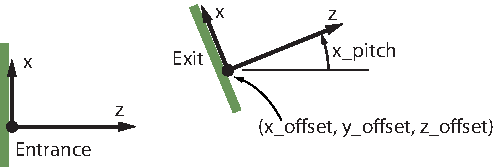
\includegraphics[width=5in]{patch.pdf}
  \caption[Patch Element.]
{A) A \vn{patch} element can align its exit face arbitrarily with respect to its entrance face. The
red arrow illustrates a possible particle trajectory form entrance face to exit face. B) The
reference length of a \vn{patch} element, if \vn{ref_coords} is set to the default value of
\vn{exit_end}, is the longitudinal distance from the entrance origin to the exit origin using the
reference coordinates at the exit end as shown. If \vn{ref_coords} is set to \vn{entrance_end}, the
length of the patch will be equal to the \vn{z_offset}.}
  \label{f:patch}
\end{figure}

%-----------------

A \vn{patch} element shifts the reference orbit and time. Also see \vn{floor_shift}
(\sref{s:floor.ele}) and \vn{fiducial} (\sref{s:fiducial}) elements. A common application of a patch
is to orient two lines with respect to each other. For example, to orient an injection line with the
ring it is injecting into (\sref{s:ex.inj}).

General \vn{patch} element attributes are:
\begin{center}
\tt
\begin{tabular}{llll} \toprule
  {\sl Attribute Class}      & Section           & {\sl Attribute Class}      & Section         \\ \midrule
  Aperture limits            & \ref{s:limit}     & Offsets, pitches \& tilt   & \ref{s:offset}  \\ 
  Chamber wall               & \ref{s:wall}      & Reference energy           & \ref{s:energy}  \\
  Custom Attributes          & \ref{s:cust.att}  & Superposition              & \ref{s:super}   \\
  Description strings        & \ref{s:alias}     & Tracking \& transfer map   & \ref{c:methods} \\
  Length                     & \ref{s:l}         &                            &                 \\
  \bottomrule
\end{tabular}
\end{center}
\toffset
See \sref{s:list.patch} for a full list of element attributes along with a their units.

\index{flexible}\index{e_tot_offset}
\index{x_offset}\index{y_offset}\index{z_offset}\index{tilt}
\index{x_pitch}\index{y_pitch}\index{t_offset}
\index{e_tot_set}\index{p0c_set}
Attributes specific to a \vn{patch} elements are:
\begin{example}
  x_offset        = <Real>    ! Exit face offset from Entrance.
  y_offset        = <Real>    ! Exit face offset from Entrance.
  z_offset        = <Real>    ! Exit face offset from Entrance.
  t_offset        = <Real>    ! Reference time offset.
  x_pitch         = <Real>    ! Exit face orientation from Entrance.
  y_pitch         = <Real>    ! Exit face orientation from Entrance.
  tilt            = <Real>    ! Exit face orientation from Entrance.
  E_tot_offset    = <Real>    ! Reference energy offset (eV).
  E_tot_set       = <Real>    ! Reference energy at exit end (eV).
  flexible        = <T/F>     ! Default: False.
  p0c_set         = <Real>    ! Reference momentum at exit end (eV).
  ref_coords      = <Switch>  ! Coordinate system defining the length.
  user_sets_length = <T/F>    ! User sets element length? Default is F.
  l               = <Real>    ! Reference length. 
\end{example}
\index{x_offset}

A straight line element like a \vn{drift} or a \vn{quadrupole} has the exit face parallel to the
entrance face. With a \vn{patch} element, the entrance and exit faces can be arbitrarily oriented
with respect to one another as shown in \fig{f:patch}A.

\index{rigid patch}\index{inflexible patch}
\index{flexible patch}
There are two different ways the orientation of the exit face is determined. Which way is used is
determined by the setting of the \vn{flexible} attribute.  With the \vn{flexible} attribute set to
\vn{False}, the default, The exit face of the \vn{patch} will be determined from the offset, tilt
and pitch attributes as described in \sref{s:patch.coords}. This type of \vn{patch} is called
``rigid'' or ``inflexible'' since the geometry of the \vn{patch} is solely determined by the
\vn{patch}'s attributes as set in the lattice file and is independent of everything else. Example:
\begin{example}
  pt: patch, z_offset = 3.2   ! Equivalent to a drift
\end{example}

With \vn{flexible} set to \vn{True}, the exit face is taken to be the reference frame of the
entrance face of the next element in the lattice. In this case, it must be possible to compute the
reference coordinates of the next element before the reference coordinates of the \vn{patch} are
computed. A \vn{flexible} \vn{patch} will have its offsets, pitches, and tilt as dependent
parameters (\sref{s:depend}) and these parameters will be computed appropriately. Here the
\vn{patch} is called ``flexible'' since the geometry of the patch will depend upon the geometry of
the rest of the lattice and, therefore, if the geometry of the rest of the lattice is modified (is
``flexed''), the geometry of the \vn{patch} will vary as well. See Section~\sref{s:ex.erl} for an
example.

The coordinates of the lattice element downstream of a \vn{flexible} \vn{patch} can be computed
if there is a \vn{fiducial} element (\sref{s:fiducial}) somewhere downstream or if there is a
\vn{multipass_slave} (\sref{s:multipass}) element which is just downstream of the \vn{patch} or at
most separated by zero length elements from the \vn{patch}. In this latter case, the
\vn{multipass_slave} must represent an $N$\Th pass slave with $N$ greater than 1. This works since
the first pass slave will be upstream of the \vn{patch} and so the first pass slave will have its
coordinates already computed and the position of the downstream slave will be taken to be the same
as the first pass slave. Notice that, without the \vn{patch}, the position of multipass slave
elements are independent of each other.

With \vn{bmad_standard} tracking (\sref{s:tkm}) A particle, starting at the upstream face of the
\vn{patch}, is propagated in a straight line to the downstream face and the suitable coordinate
transformation is made to translate the particle's coordinates from the upstream coordinate frame to
the downstream coordinate frame (\sref{s:patch.std}). In this case the \vn{patch} element can be
thought of as a generalized \vn{drift} element.

If there are magnetic or electric fields within the \vn{patch}, the tracking method through the
\vn{patch} must be set to either \vn{runge_kutta} or \vn{custom}. Example:
\begin{example}
  pa2: patch, tracking_method = runge_kutta, field_calc = custom, 
              mat6_calc_method = tracking, ...
\end{example}
In order to supply a custom field when \vn{runge_kutta} tracking is used, \vn{field_calc}
(\sref{s:integ}) needs to be set to \vn{custom}. In this case, custom code must be supplied for
calculating the fields as a function of position (\sref{s:custom.ele}).

The \vn{E_tot_offset} attribute offsets the
reference energy:
\begin{example}
  E_tot_ref(exit) = E_tot_ref(entrance) + E_tot_offset (eV)
\end{example}
Setting the \vn{E_tot_offset} attribute will affect a particle's $p_x$, $p_y$ and $p_z$ coordinates
via \Eqs{ppp} and \eq{ppppp}.  Notice that \vn{E_tot_offset} does not affect a particle's actual
energy, it just affects the difference between the particle energy and the reference energy.

Alternatively, to set the reference energy, the \vn{E_tot_set} or \vn{p0c_set} attributes can be
used to set the reference energy/momentum at the exit end. It is is an error if more than one of
\vn{E_tot_offset}, \vn{E_tot_set} and \vn{p0c_set} is nonzero.

\vn{Important}: \bmad may apply the energy transformation either before or after the coordinate
transformation. This matters when the speed of the reference particle is less than $c$. For this
reason, and due to complications involving PTC, it is recommended to use two patches in a row when
both the orbit and energy are to be patched.

A \vn{patch} element can have an associated electric or magnetic field (\sref{s:fieldmap}). This can
happen, for example, if a patch is used at the end of an injection line to match the reference
coordinates of the injection line to the line being injected into (\sref{s:ex.inj}) and the patch
element is within the field generated by an element in the line being injected into. In such a case,
it can be convenient to set what the reference coordinates are since the orientation of any fields
that are defined for a patch element will be oriented with respect to the patch element's reference
coordinates. For this, the \vn{ref_coords}
parameter of a patch can be used. Possible settings are:
\vn{ref_coords} are:
\begin{example}
  entrance_end  !
  exit_end      ! Default
\end{example}
The default setting of \vn{ref_coords} is \vn{exit_end} and with this the reference coordinates are
set by the exit end coordinate system (see \fig{f:patch}). If \vn{ref_coords} is set to
\vn{entrance_end}, the reference coordinates are set by the entrance end coordinate system. Example:
\begin{example}
  p1: patch, x_offset = 1, x_pitch = 0.4   ! L = 0.289418 see below
  p2: p1, ref_coords = entrance_end        ! L = 0
\end{example}
Here \vn{p1} has \vn{ref_coords} set to \vn{exit_end} (the default). \vn{p2} inherits the parameters
of \vn{p1} and sets \vn{ref_coords} to \vn{entrance_end}.

It is important to keep in mind that if there are multiple patches in a row, while two different
configurations may be the same in a geometrical sense the total length may not be the same. For
example:
\begin{example}
  pA: patch, x_offset = 1    ! L = 0
  pB: patch, x_pitch = 0.4   ! L = 0
  sum: line = (pA, pB)
\end{example}
The configuration of \vn{pA} followed by \vn{pB} is equivalent geometrically to the \vn{p1} patch
above but the total length of the \vn{(pA, pB)} line is zero which is different from the length of
\vn{p1}.

Unfortunately, there is no intuitive way to define the ``\vn{length}'' \vn{L} of a patch. This is
important since the transit time of the reference particle is the element length divided by the
reference velocity. And the reference transit time will affect how the phase space $z$ coordinate
changes through the patch via \Eq{zbctt}. If the parameter \vn{user_sets_length} is set to True, the
value of \vn{l} set in the lattice file will be used (default is zero). \vn{user_sets_length} is set
to False (the default), the length of a patch is calculated depending upon the setting of
\vn{ref_coords}.  If \vn{ref_coords} is set to \vn{exit_end}, the length of the patch is calculated
as the perpendicular distance between the origin of the patch's entrance coordinate system and the
exit face of the patch as shown in \fig{f:patch}B. If \vn{ref_coords} is set to \vn{entrance_end},
the length is calculated as the perpendicular distance between the entrance face and the origin of
the exit coordinate system. In this case, the length will be equal to \vn{z_offset}.

To provide flexibility, the \vn{t_offset} attribute can be
used to offset the reference time. The reference time at the exit end of the patch
\vn{t_ref(exit)} is related to the reference time at the beginning of the patch \vn{t_ref(entrance)}
via
\begin{example}
  t_ref(exit) = t_ref(entrance) + t_offset + dt_travel_ref
\end{example}
where \vn{dt_travel_ref} is the time for the reference particle to travel through the patch.
\vn{dt_travel_ref} is defined to be:
\begin{example}
  dt_travel_ref = L / beta_ref
\end{example}
Where \vn{L} is the length of the \vn{patch} and \vn{beta_ref} is the reference velocity/c at the
exit end of the element. That is, the reference energy offset is applied {\em before} the reference
particle is tracked through the patch. Since this point can be confusing, it is recommended that a
\vn{patch} element be split into two consecutive patches if the \vn{patch} has finite \vn{l} and
\vn{E_tot_offset} values.

While a finite \vn{t_offset} will affect the reference time at the end of a patch, a finite
\vn{t_offset} will {\em not} affect the time that is calculated for a particle to reach the end of
the patch. On the other hand, a finite \vn{t_offset} will affect a particle's $z$ coordinate via
\Eqs{zbctt}. The change in $z$, $\delta z$ will be
\begin{equation}
  \delta z = \beta \cdot c \cdot \text{t_offset}
\end{equation}
where $\beta$ is the normalized particle speed (which is independent of any energy patch). Another
way of looking at this is to note that In a drift, if the particle is on-axis and on-energy, t and
t_ref change but z does not change. In a time patch (a patch with only \vn{t_offset} finite), t_ref
and z change but t does not.

When a lattice branch contains both normally oriented and reversed elements
(\sref{s:ref.construct}), a \vn{patch}, or series of \vn{patches}, which reflects the $z$ direction
must be placed in between. Such a \vn{patch}, (or patches) is called a \vn{reflection} \vn{patch}.
See Section~\sref{s:reflect.patch} for more details on how a reflection patch is defined. In order
to avoid some confusing conceptual problems involving the coordinate system through a reflection
patch, Runge-Kutta type tracking is prohibited with a reflection patch.\footnote
  {
In general, Runge-Kutta type tracking through a patch is a waste of time unless electric or magnetic
fields are present.
  }

\index{wall}
Since the geometry of a \vn{patch} element is complicated, interpolation of the chamber wall in the
region of a patch follows special rules. See section~\sref{s:wall.vacuum} for more details.

\newpage

%-----------------------------------------------------------------
\section{Photon_Init}
\label{s:photon.init}
\index{photon_init|hyperbf}

A \vn{photon_init} element is used as a starting element for x-ray tracking.  A \vn{photon_init}
element can be used to define such things as the initial energy spectrum and angular orientation. As
explained below, a \vn{photon_init} element can be a ``stand alone'' photon source or it can have an
associated ``physical source'' element.

Note: There is a utility program called \vn{photon_init_plot} that comes with a Bmad Distribution
that will plot initial photon distributions and can be used as a check.

General \vn{photon_init} attributes are:
\begin{center}
\tt
\begin{tabular}{llll} \toprule
  {\sl Attribute Class}      & Section           & {\sl Attribute Class}      & Section         \\ \midrule
  Aperture limits            & \ref{s:limit}     & Length                     & \ref{s:l}       \\
  Chamber wall               & \ref{s:wall}      & Offsets, pitches \& tilt   & \ref{s:offset}  \\
  Custom Attributes          & \ref{s:cust.att}  & Reference energy           & \ref{s:energy}  \\ 
  Description strings        & \ref{s:alias}     & Tracking \& transfer map   & \ref{c:methods} \\ 
  \bottomrule
\end{tabular}
\end{center}
\toffset
See \sref{s:list.photon.init} for a full list of element attributes along with a their units.

\index{x_half_length}\index{y_half_length}
Attributes specific to an \vn{photon_init} element are:
\begin{example}
  ds_slice                 = <Real>
  E_center                 = <Real>    ! Average init photon energy of 1st mode (eV).
  E2_center                = <Real>    ! Average init photon energy of 2nd mode (eV).
  E2_probability           = <Real>    ! Probability of 2nd mode.
  E_center_relative_to_ref = <T/F>     ! E_center relative to reference E? Default True.
  e_field_x                = <Real>    ! Polarization. x & y = 0 -> random
  e_field_y                = <Real>
  energy_distribution      = <Switch>  ! Gaussian, uniform, or curve.
  energy_probability_curve = \{...\}   ! Used with energy_distribution = curve. See below.
  physical_source          = <String>  ! physical source of x-rays
  ref_wavelength                       ! Ref wavelength (\sref{s:energy}). Dep attribute (\sref{s:depend}).
  sig_x                    = <Real>
  sig_y                    = <Real>
  sig_z                    = <Real>
  sig_vx                   = <Real>
  sig_vy                   = <Real>
  sig_E                    = <Real>    ! Init photon energy width of 1st mode (eV).
  sig_E2                   = <Real>    ! Init photon energy width of 2nd mode (eV).
  spatial_distribution     = <Switch>  ! Gaussian or uniform. 
  transverse_sigma_cut     = <Real>
  velocity_distribution    = <Switch>  ! Gaussian, spherical, or uniform. 
\end{example}

When the \vn{energy_distribution} is set to \vn{gaussian} or \vn{uniform}, the distribution of
photons is bimodal. The first mode is characterized by the parameters \vn{E_center}, and \vn{sig_E},
the second mode is characterized by the parameters \vn{E2_center} and \vn{sig_E2}. The probability
of emitting a photon in the second mode is given by \vn{E2_probability}.

\begin{description}
%
  \index{ds_slice}
  \item[\vn{ds_slice}] \Newline
Used when there is an associated physical source element. The physical source element is sliced into
pieces of thickness \vn{ds_slice} and each slice is tested to see if photons from the slice can
possibly pass through the first aperture. When photons are generated, photons will only be generated
from slices where they have a hope of passing through the first aperture. This makes the simulation
more efficient.  The default value of \vn{ds_slice} is 0.01 meter.
%
  \index{E_center}\index{E2_center}
  \item[\vn{E_center}, \vn{E2_center}] \Newline
Average initial photon energy in eV. If \vn{E_center_relative_to_ref} is set to True, \vn{E_center}
and \vn{E2_center} will be relative to the reference energy.
%
  \index{E_center_relative_to_ref}
  \item[\vn{E_center_relative_to_ref}] \Newline
With a setting of True (the default), \vn{E_center} and \vn{E2_center} are taken to be with respect
to the reference energy (\sref{s:ref.energy}). That is, if True, the center energy \vn{<E>} is
\begin{example}
  <E-1st-mode> = E1_center + Reference_Energy
  <E-2nd-mode> = E2_center + Reference_Energy
\end{example}
If \vn{E_center_relative_to_ref} is set to False, \vn{E_center} and \vn{E2_center} are taken to be
the center energy values independent of the reference energy.
%
  \index{E2_probability}
  \item[\vn{E2_probability}] \Newline
Probability of emitting a photon from the 2nd mode. A value of 0 (the default) will mean
that all photons will be emitted from the 1st mode and a value of 1 will mean that
all photons will be emitted from the 2nd mode.
%
  \index{e_field_x}\index{e_field_y}
  \item[\vn{e_field_x}, \vn{e_field_y}] \Newline
Electric field component of initial photons in the $x$ and $y$ planes. If both are set to 0 then a
random field is chosen with unit intensity $E_x^2 + E_y^2 = 1$.
%
  \index{energy_distribution}
  \item[\vn{energy_distribution}] \Newline
Sets the type of energy spectrum for emitted photons. If there is an associated physical element
then this parameter is ignored and the energy distribution is calculated from the properties of the
physical element. Possible settings are:
\begin{example}
  gaussian   ! Default
  uniform
  curve
\end{example}
The \vn{gaussian} setting gives Gaussian distributions for the two modes with width set by
\vn{sig_E} and \vn{sig_E2}. The \vn{uniform} setting gives a flat distribution in the range:
\begin{example}
  [-sig_E, sig_E]    ! For the 1st mode
  [-sig_E2, sig_E2]  ! For the 2nd mode
\end{example}
The \vn{curve} setting uses the energy probability curve set by the \vn{energy_probability_curve}
component.
%
  \index{energy_probability_curve}
  \item[\vn{energy_probability_curve}] \Newline
The \vn{energy_probability_curve} attribute provides a way to specify the energy probability
distribution when an Gaussian or uniform distribution is not suitable. The probability curve is
defined by specifying the curve at a number of points. The syntax is:
\begin{example}
  energy_probability_curve = \{E1 p1, E2 p2, ..., EN pN\}
\end{example}
where the \vn{E p} pairs are the energy and photon emissian probability at that energy. 
The commas between \vn{E p} pairs is optional.
The probability curve does not have to be normalized, \bmad will take care of that. \bmad will
use cubic spline interpolation between points. 
%
  \index{physical_source}
  \item[\vn{physical_source}] \Newline
Used to specify the ``physical'' source of the photons. See below for more details
%
  \index{sig_E}\index{sig_E2}
  \item[\vn{sig_E}, \vn{sig_E2}] \Newline
Energy width of the two modes in eV. See \vn{energy_distribution} for more details.
%
  \index{sig_vx}\index{sig_vy}
  \item[\vn{sig_vx, sig_vy}] \Newline
Width of emitted photons in $v_x/c$ and $v_y/c$ directions. See
\vn{velocity_distribution} for more details.
%
  \index{sig_x}\index{sig_y}\index{sig_z}
  \item[\vn{sig_x, sig_y, sig_z}] \Newline
Width of emitted photons in $x$, $y$ and $z$ directions. See
\vn{spatial_distribution} for more details.
%
  \index{spatial_distribution}
  \item[\vn{spatial_distribution}] \Newline
Sets spacial $(x, y, z)$ spectrum of emitted photons. If there is an associated physical element
then this parameter is ignored and the energy distribution is calculated from the properties of the
physical element. Possible settings are:
\begin{example}
  gaussian    ! Default
  uniform
\end{example}
The \vn{gaussian} setting gives a Gaussian distribution with width
$\sigma$ where $\sigma$ is 
\begin{example}
  sig_x     ! for x distribution
  sig_y     ! for y distribution
  sig_z     ! for z distribution
\end{example}
The \vn{uniform} setting gives a flat
distribution in the range: $[-\sigma, \sigma]$.
%
  \index{velocity_distribution}
  \item[\vn{velocity_distribution}] \Newline
Sets the transverse $(v_x/c, v_y/c)$ velocity spectrum of emitted photons. If there is an associated
physical element then this parameter is ignored and the energy distribution is calculated from the
properties of the physical element. The longitudinal velocity is always computed to make $v_x^2 +
v_y^2 + v_z^2 = c^2$ Possible settings are:
\begin{example}
  gaussian    ! Default
  spherical
  uniform
\end{example}
The \vn{gaussian} setting gives a Gaussian distribution with width
$\sigma$ where $sigma$ is 
\begin{example}
  sig_vx     for vx/c distribution
  sig_vy     for vy/c distribution
\end{example}
The \vn{uniform} setting gives a flat distribution in the range: $[-\sigma, \sigma]$. The
\vn{spherical} setting gives flat distribution in all directions. With the \vn{spherical}
setting is used, and the next downstream element excluding drifts and markers is an element
with aperture limits (\sref{s:limit}), \bmad can optimize photon emission to only emitting 
photons that are very likely to be within the aperture when they hit the downstream element.
This cuts down on computation time.
%
\end{description}

For the purposes of positioning the elements in the lattice around it,
a \vn{photon_init} element is considered to have zero length.

\vn{photon_init} elements are used in one of two modes: With or without an associated physical
source element specified by the \vn{physical_source} attribute. Without an associated physical
source, the \vn{photon_init} element completely specifies the initial photon distribution. With an
associated physical source element, the photon distribution is determined by the properties of the
physical source but the shape of the energy spectrum can be modified by setting attributes in the
\vn{photon_init} element. Example:
\begin{example}
  b05w: sbend, l = 3.2, angle = 0.1
  pfork: photon_fork, to_line = c_line, superimpose, ref = b05w, offset = 0.4
  bend_line: line = (..., b05w, ...)
  use bend_line

  c_line: line = (pinit, ...)
  c_line[E_tot] = 15e3
  pinit: photon_init, physical_source = "b05w", sig_E = 2.1
\end{example}
In this example, the bend \vn{b05w} is a bend producing photons. It is part of the line
\vn{bend_line}. \vn{bend_line} also contains a \vn{photon_fork} element named \vn{pfork} which
branches to the line \vn{c_line}. \vn{c_line} contains the \vn{photon_init} element \vn{pinit} which
references \vn{b03w} as the associated physical source element. When photons are tracked, they are
generated in \vn{b05w} and then propagated to the \vn{pfork} fork.  After this they are propagated
through \vn{c_line}. The \vn{pinit} element acts like a zero length \vn{marker} element when photons
propagate through it. That is, the \vn{pinit} element essentially serves to associate \vn{c_line}
with \vn{b03w} for the purposes of photon tracking. Also, in this example, \vn{pinit} modifies the
photon energy spectrum so that only photons whose energy is within 2.1 eV are generated

It is important to note that in the above example, with the \vn{photon_init} element having an
associated physical source, the setting of things like the spatial shape \vn{sig_z}, etc. in the
\vn{photon_init} element will be ignored.

See Section~\sref{s:rowland} for an example lattice that can be used to simulate a Rowland circle
spectrometer using a \vn{photon_init} element.

\newpage

%-----------------------------------------------------------------
\section{Quadrupole}
\label{s:quad}
\index{quadrupole|hyperbf}

A \vn{quadrupole} is a magnetic element with a linear field dependence
with transverse offset (\sref{s:mag.field}).

General \vn{quadrupole} attributes are:
\begin{center}
\tt
\begin{tabular}{llll} \toprule
  {\sl Attribute Class}      & Section           & {\sl Attribute Class}      & Section            \\ \midrule
  Aperture limits            & \ref{s:limit}     & Mag \& Elec multipoles     & \ref{s:multip}     \\
  Chamber wall               & \ref{s:wall}      & Offsets, pitches \& tilt   & \ref{s:offset}     \\
  Description strings        & \ref{s:alias}     & Overlapping Fields         & \ref{s:overlap}    \\
  Fringe Fields              & \ref{s:fringe}    & Reference energy           & \ref{s:energy}     \\ 
  Hkick \& Vkick             & \ref{s:kick}      & Superposition              & \ref{s:super}      \\
  Integration settings       & \ref{s:integ}     & Symplectify                & \ref{s:symp}       \\
  Is_on                      & \ref{s:is.on}     & Field Maps                 & \ref{s:fieldmap}   \\ 
  Length                     & \ref{s:l}         & Tracking \& transfer map   & \ref{c:methods}    \\ 
  \bottomrule
\end{tabular}
\end{center}
\toffset
See \sref{s:list.quadrupole} for a full list of element attributes along with a their units.

\index{f1}\index{f2}
\index{k1}\index{b1_gradient}
Attributes specific to a \vn{quadrupole} element are:
\begin{example}
  b1_gradient  = <Real>    ! Field strength. (\sref{s:depend}).
  k1           = <Real>    ! Quadrupole strength.
  fq1          = <Real>    ! Soft edge fringe parameter.
  fq2          = <Real>    ! Soft edge fringe parameter.
  field_master = <T/F>     ! See \sref{s:field.master}.
 \end{example}
The normalized quadrupole \vn{k1} strength is related to the unnormalized \vn{b1_gradient} field
strength through \Eq{kqlbp}.

\index{tilt}
If the \vn{tilt} attribute is present without a value then a value of $\pi/4$
is used.

For a quadrupole with zero \vn{tilt} and a positive \vn{k1}, the
quadrupole is horizontally focusing and vertically defocusing
(\sref{s:mag.field}).

The \vn{fq1} and \vn{fq2} parameters are used to specify the
quadrupolar ``soft'' edge fringe. See \sref{s:q.soft} for more details.
The \vn{fringe_at} and \vn{fringe_type} settings (\sref{s:fringe})
determine if the fringe field is used in tracking (\sref{s:fringe}).

Example:
\begin{example}
  q03w: quad, l = 0.6, k1 = 0.003, tilt  ! same as tilt = pi/4
\end{example}

\newpage

%-----------------------------------------------------------------------------
\section{Ramper}
\label{s:ramper}
\index{ovlerlay|hyperbf}

A \vn{ramper} element is a type of \vn{control} element (\sref{s:lord.slave}). That is, a
\vn{ramper} element can be used to make variations in the attributes of other elements while a
program is running. The \vn{ramper} element is similar to an \vn{overlay} element except that
\vn{ramper} elements are designed to control large sets of elements. Also \vn{ramper} elements can
be used to smoothly vary parameters as particle are propagated through a lattice. \vn{Ramper}
elements where implemented to solve the problem of simulating machine ramping where the strength of
many elements in a machine are varied continuously as a function of time. The drawback of
\vn{ramper} elements is that they can be only be used with programs that that are designed to handle
them.\footnote
  {
In particular, the \vn{long_term_tracking} program that is bundled with the \bmad software
(\sref{s:tao.intro}) can handle \vn{ramper} elements.
  }
Ramper elements will be ignored in programs that are not designed to handle them. How a program
handles ramper elements will be program dependent and the program documentation should be consulted
for details.

Note: \vn{ac_kicker} elements can also be used for simulating a time dependent element.

General \vn{ramper} attributes are:
\begin{center}
\tt
\begin{tabular}{llll} \toprule
  {\sl Attribute Class}      & Section           & {\sl Attribute Class}      & Section         \\ \midrule
  Custom Attributes          & \ref{s:cust.att}  & Is_on                      & \ref{s:is.on}   \\
  Description strings        & \ref{s:alias}     &                            &                 \\ 
  \bottomrule
\end{tabular}
\end{center}
\toffset
See \sref{s:list.ramper} for a full list of element attributes.

The syntax for \vn{ramper} elements is exactly the same as for \vn{overlay} (\sref{s:go.syntax}) elements 
except that \vn{ramper} elements do not have a \vn{gang} attribute.

Like \vn{overlay}s, There are two types of \vn{ramper} elements: \vn{Expression} based and
\vn{knot} based.  The general syntax for a \vn{expression} based \vn{ramper} element is
\begin{example}
  name: RAMPER = \{ele1[attrib1]:coef1, ele2[attrib2]:coef2, ...\}, VAR = \{var1\}
\end{example}
where \vn{ele1[attrib1]}, \vn{ele2[attrib2]}, etc. specify the slave attributes and \vn{exp1},
\vn{exp2}, etc. are the arithmetical expressions, that are functions of \vn{var1}, \vn{var2}, etc.,
and are used to determine a value for the slave attributes.

The general syntax for a \vn{knot} based  \vn{ramper} element is
\begin{example}
  name: RAMPER = \{ele1[attrib1]:\{y_knot_points1\}, ele2[attrib2]:\{y_knot_points2\}, ...\}, 
              VAR = \{var1\}, X_KNOT = \{x_knot_points\}, INTERPOLATION = \{type\},
              var1 = init_val1, ...
\end{example}

\textbf{See Section~\sref{s:go.syntax} for a detailed description of this syntax.}

Examples:
\begin{example}
  ramp_e: ramper = \{*[e_tot]:\{4e+08, 4.00532e+08, 4.01982e+08, ...\}\},
                var = \{time\}, x_knot = \{0, 0.001, 0.002, ...\}, interpolation = cubic

  amp = 1e9;  omega = 0.167;  t0 = 0.053
  ramp_rf: ramper = \{rfcavity::*[voltage]:amp*sin(omega *(t + t0)),
        rfcavity::*[phi0]:0.00158*t^2 + 3*q\}, var = \{t, q\}
\end{example}
\vn{Ramp_e} uses a cubic spline fit to interpolate between the knot points specified in the element
definition.  The ``\vn{*[e_tot]}'' construct in the definition of \vn{ramp_e} means that the ramper
will be applied to the \vn{e_tot} attribute (\sref{s:energy}) of all elements (since the wild card
character ``\vn{*}'' (\sref{s:ele.match}) will match to all element names).

The \vn{ramp_rf} ramper in the above example varies the \vn{voltage} and \vn{phase} (\vn{phi0})
attributes of all elements that match to \vn{rfcavity::*}. That is, all \vn{rfcavity} elements. Here
mathematical expressions are used instead of knot points.

\vn{Ramper} elements can control the variables of other controller element except \vn{rampers} are
not allowed to control \vn{rampers}. When a \vn{ramper} controls variables in other controller
elements it is not permitted to use wild card characters. That is, in the above example, ``\vn{*}''
will not match to any controller elements.

If a slave name contains wild card characters, for a given lattice element that the slave name
matches to, it is not required that the controlled attribute be a valid attribute of the element. In
the case where the controlled attribute is not valid for a given lattice element, no attributes of
the given lattice element are varied when and the ramper is varied. For example:
\begin{example}
  rz: ramper = \{*[k1]: ...
\end{example}
In this example the \vn{k1} attribute of all those elements that have a \vn{k1} attribute will be
controlled but something like a \vn{sextupole} element which does not have a \vn{k1} attribute will
not be controlled.

Due to the way bookkeeping is done for ramper elmeents, and unlike \vn{group} or \vn{overlay}
elements, it is not permitted for different \vn{ramper} elements to control the same parameter of a
given slave element. Additionally, parameters that \vn{ramper} elements control must not be
controlled by any \vn{overlay} (but a \vn{ramper} can control an \vn{overlay}).

Note: There is a program to plot controller response curves bundled with the \bmad software
(\sref{s:tao.intro}) called \vn{controller_function_plot}. Documentation on this can
be found at:
\begin{example}
  util_programs/controller_function_plot
\end{example}

\newpage

%-----------------------------------------------------------------
\section{RF_bend}
\label{s:rf.bend}
\index{rf_bend|hyperbf}

An \vn{rf_bend} is an RF cavity with the geometry of an \vn{sbend} (\sref{s:bend}). This element is
currently considered to be experimental so please contact a \bmad maintainer if you want to use this
type of element.

General \vn{rfcavity} attributes are:
\begin{center}
\tt
\begin{tabular}{llll} \toprule
  {\sl Attribute Class}      & Section            & {\sl Attribute Class}      & Section            \\ \midrule
  Aperture limits            & \ref{s:limit}      & Offsets, pitches \& tilt   & \ref{s:offset}     \\
  Chamber wall               & \ref{s:wall}       & Overlapping Fields         & \ref{s:overlap}    \\
  Custom Attributes          & \ref{s:cust.att}   & Reference energy           & \ref{s:energy}     \\ 
  Description strings        & \ref{s:alias}      & Superposition              & \ref{s:super}      \\
  Symplectify                & \ref{s:symp}       & Field Maps                 & \ref{s:fieldmap}   \\
  Integration settings       & \ref{s:integ}      & Tracking \& transfer map   & \ref{c:methods}    \\
  Is_on                      & \ref{s:is.on}      & Wakes                      & \ref{s:wakes}      \\
  Length                     & \ref{s:l}          &                            &                    \\
  \bottomrule
\end{tabular}
\end{center}
\toffset
See \sref{s:list.rf.bend} for a full list of element attributes along with a their units.

\index{rf_frequency}\index{harmon}\index{voltage}\index{phi0}\index{phi0_multipass}
Attributes specific to an \vn{rf_bend} are:
\begin{example}
  ! Bend-like attributes:
  angle              = <Real>   ! Design bend angle. Dependent var (\sref{s:depend}).
  b_field            = <Real>   ! Design field strength (= P_0 g / q) (\sref{s:depend}).
  g                  = <Real>   ! Design bend strength (= 1/rho).
  l                  = <Real>   ! "Length" of bend. See below.
  l_arc              = <Real>   ! Arc length. For \vn{rbend}s only. 
  l_chord            = <Real>   ! Chord length. See \sref{s:l}.
  l_sagitta                     ! Sagittal length. Dependent param (\sref{s:depend}).
  rho                = <Real>   ! Design bend radius. Dependent param (\sref{s:depend}).
  roll               = <Real>   ! See \ref{s:offset}.
  field_master       = <T/F>    ! See \ref{s:field.master}.

  ! RF-like attributes:
  rf_frequency    = <Real>    ! Frequency
  harmon          = <Real>    ! Harmonic number
  harmon_master   = <Logic>   ! Is harmon or rf_frequency the dependent var with ref energy changes?
  phi0            = <Real>    ! Cavity phase (rad/2pi).
  phi0_multipass  = <Real>    ! Phase variation with multipass (rad/2pi).
\end{example}

Tracking through an \vn{rf_bend} is limited to Runge Kutta like tracking methods (\sref{s:tkm}). The
default \vn{tracking_method} is \vn{runge_kutta}. Fields must be specified using a grid field map
(\sref{s:fieldmap}). The default \vn{field_calc} is \vn{fieldmap} (\sref{s:field.calc}).

The geometry of the \vn{rf_bend} is the same as an \vn{sbend}. An \vn{rf_bend} has a sector shape
which is equivalent to \vn{e1} and \vn{e2} being zero for an \vn{sbend}. Since the fields are specified
using a grid field map, there are no fringe attributes to set (for any elements where a grid field is
used, it is always assumed that the fringe fields are included as part of the grid field).

\newpage

%-----------------------------------------------------------------
\section{RFcavity}
\label{s:rfcav}
\index{rfcavity|hyperbf}

An \vn{rfcavity} is an RF cavity without acceleration generally used in a storage ring. The main
difference between an \vn{rfcavity} and an \vn{lcavity} is that, unlike an \vn{lcavity}, the
reference energy (\sref{s:phase.space}) through an \vn{rfcavity} is constant.

General \vn{rfcavity} attributes are:
\begin{center}
\tt
\begin{tabular}{llll} \toprule
  {\sl Attribute Class}      & Section            & {\sl Attribute Class}      & Section            \\ \midrule
  Aperture limits            & \ref{s:limit}      & Offsets, pitches \& tilt   & \ref{s:offset}     \\
  Chamber wall               & \ref{s:wall}       & Overlapping Fields         & \ref{s:overlap}    \\
  Custom Attributes          & \ref{s:cust.att}   & Reference energy           & \ref{s:energy}     \\ 
  Description strings        & \ref{s:alias}      & RF Couplers                & \ref{s:rf.coupler} \\
  Field autoscaling          & \ref{s:autoscale}  & Superposition              & \ref{s:super}      \\
  Fringe Fields              & \ref{s:fringe}     & Symplectify                & \ref{s:symp}       \\
  Hkick \& Vkick             & \ref{s:kick}       & Field Maps                 & \ref{s:fieldmap}   \\
  Integration settings       & \ref{s:integ}      & Tracking \& transfer map   & \ref{c:methods}    \\
  Is_on                      & \ref{s:is.on}      & Wakes                      & \ref{s:wakes}      \\
  Length                     & \ref{s:l}          &                            &                    \\
  \bottomrule
\end{tabular}
\end{center}
\toffset
See \sref{s:list.rfcavity} for a full list of element attributes along with a their units.

\index{rf_frequency}\index{harmon}\index{voltage}\index{phi0}\index{phi0_multipass}
Attributes specific to an \vn{rfcavity} are:
\begin{example}
  rf_frequency    = <Real>    ! Frequency
  harmon          = <Real>    ! Harmonic number
  harmon_master   = <Logic>   ! Is harmon or rf_frequency the dependent var with ref energy changes?
  voltage         = <Real>    ! Cavity voltage
  phi0            = <Real>    ! Cavity phase (rad/2pi).
  phi0_multipass  = <Real>    ! Phase variation with multipass (rad/2pi).
  phi0_autoscale  = <Real>    ! Set by Bmad if autoscaling is turned on (rad/2pi).
  gradient        = <Real>    ! Accelerating gradient (V/m). Dependent attribute (\sref{s:depend}).
  longitudinal_mode = <Int>   ! Longitudinal mode. Default is 1. May be 0 or 1.
\end{example}

The integrated energy kick felt by a particle, assuming no phase slippage, is 
\begin{example}
  dE = -e_charge * \(r_q\) * voltage * sin(\(2\,\pi\) * (\(\phi_\text{t}\) - \(\phi_\REF\)))
\end{example}
\index{multipass}
where
\begin{example}
  \(\phi_\REF\) = phi0 + phi0_multipass + phi0_autoscale
  \label{rfcav.phi}
\end{example}
and $\phi_t$ is the part of the phase due to when the particle arrives at the cavity and depends
upon whether \vn{absolute time tracking} or \vn{relative time tracking} is being used as discussed
in \sref{s:rf.time}.

In the above equation $r_q$ is the relative charge between the reference particle (set by the
\vn{parameter[particle]} parameter in a lattice file) and the particle being tracked through the
cavity. For example, if the reference particle and and the tracked particle are the same, $r_q$ is
unity independent of the type of particle tracked.

The correspondence between the \bmad \vn{phi0} attribute and the \vn{lag} attribute of
\mad is
\begin{example}
  phi0 = mad + 0.5
\end{example}

\vn{phi0_multipass} is only to be used to shift the phase with respect to a \vn{multipass} lord. See
\sref{s:multipass}. \vn{e_charge} is the magnitude of the charge on an electron
(Table~\ref{t:constants}). Notice that the energy kick is independent of the sign of the charge of
the particle

\vn{phi0_autoscale} and \vn{field_autoscale} are calculated by \bmad's auto-scale module. See
Section~\sref{s:autoscale} for more details. Autoscaling can be toggled on/off by using the
\vn{autoscale_phase} and \vn{autoscale_amplitude} toggles.

Note: Zero phase for $\phi_\REF$ corresponds to the stable fixed point above transition.

Note: \vn{Phi0} is not to be confused with the synchronous phase. The synchronous phase is the phase
of the particle as it passes through the cavity with respect to the RF waveform. The synchronous
phase is not something that is set by the User but rather is established by the balance between the
energy gain of the particle as it goes through the cavities in the ring versus the energy lost to
synchrotron radiation. In fact, for a ring with a single cavity, the synchronous phase is independent
of \vn{phi0}. Changing \vn{phi0} in such a situation will result in the closed orbit phase space $z$ to
vary in lock step.

If \vn{harmon} is non--zero the \vn{rf_frequency} is calculated by
\begin{example}
  rf_frequency = harmon * c_light * beta0 / L_lattice 
\end{example}
where \vn{L_lattice} is the total lattice length and \vn{beta0} is the
velocity of the reference particle at the start of the lattice. After
the lattice has been read in, \vn{rf_frequency} will be the
independent variable (\sref{s:depend}).

Couplers (\sref{s:rf.coupler}) and HOM wakes (\sref{s:wakes}) can
be modeled. In addition, if a field map is specified
(\sref{s:fieldmap}), tracking using an integrator is possible.

\index{RF field map}
\index{runge_kutta!and field maps}
\index{symp_lie_bmad!and field maps}
If a field map is specified (\sref{s:fieldmap}), tracking using an integrator is possible. A field
map is only used for \vn{runge_kutta}, \vn{fixed_step_runge_kutta}, and \vn{symp_lie_bmad} tracking
(\sref{s:tkm}). Only the fundamental mode has an analytical formula for the symplectic
tracking. With \vn{cavity_type} set to \vn{standing_wave}, the longitudinal mode is set by the
\vn{longitudinal_mode} parameter. The possible values are 0 or 1 and the default setting is 0.

The \vn{cavity_type} is the type of cavity being simulated. Possible
settings are:
\begin{example}
  ptc_standard
  standing_wave    ! Default
  traveling_wave
\end{example}
The \vn{cavity_type} switch is ignored if a field map is used.

Example:
\begin{example}
  rf1: rfcav, l = 4.5, harmon = 1281, voltage = 5e6
\end{example}

\newpage

%-----------------------------------------------------------------
\section{Sad_Mult}
\label{s:sad.mult}
\index{sad_mult|hyperbf}

A \vn{sad_mult} element is equivalent to a SAD\cite{b:sad} \vn{mult}
element. This element is a combination solenoid, multipole, bend, and
RF cavity.

General \vn{sample} attributes are:
\begin{center}
\tt
\begin{tabular}{llll} \toprule
  {\sl Attribute Class}      & Section           & {\sl Attribute Class}      & Section         \\ \midrule
  a$n$, b$n$ multipoles      & \ref{s:multip}    & Length                     & \ref{s:l}       \\
  Aperture limits            & \ref{s:limit}     & Offsets, pitches \& tilt   & \ref{s:offset}  \\
  Chamber wall               & \ref{s:wall}      & Reference energy           & \ref{s:energy}  \\ 
  Custom Attributes          & \ref{s:cust.att}  & Superposition              & \ref{s:super}   \\
  Description strings        & \ref{s:alias}     & Tracking \& transfer map   & \ref{c:methods} \\ 
  Fringe Fields              & \ref{s:fringe}    &                            &                 \\
  \bottomrule
\end{tabular}
\end{center}
\toffset
See \sref{s:list.sad.mult} for a full list of element attributes along with a their units.

\index{angle}\index{bs_field}\index{e1}\index{e2}\index{eps_step_scale}
\index{f1}\index{f2}\index{g}\index{rf_frequency}\index{harmon}
\index{ks}\index{phi0}\index{rho}\index{voltage}\index{x_offset_mult}
\index{y_offset_mult}\index{x_pitch_mult}\index{y_pitch_mult}
\index{fringe_type}\index{kill_fringe}
Attributes specific to an \vn{sad_mult} element are:
\begin{example}
  bs_field        = <Real>    ! Solenoid field. SAD equivalent: BZ.
  ks              = <Real>    ! Solenoid strength. 
  e1, e2          = <Real>    ! Bend face angles.
  eps_step_scale  = <Real>    ! Step size scale. Default = 1. SAD equivalent: EPS.
  fq1, fq2        = <Real>    ! Quadrupole fringe integral. SAD equivalents: F1, F2.
  x_offset_mult   = <Real>    ! Mult component offset. SAD equivalent: DX.
  y_offset_mult   = <Real>    ! Mult component offset. SAD equivalent: DY.
  fringe_type     = <Switch>  ! Type of fringe. SAD equivalent: DISFRIN.
  fringe_at       = <Switch>  ! Where fringe is applied. SAD equivalent: FRINGE.
\end{example}

%  angle           = <Real>    ! Bend angle. A settable dependent variable (\sref{s:depend})
%  g               = <Real>    ! Bend strength 1/rho
%  rf_frequency    = <Real>    ! RF frequency (Hz). SAD equivalent: FREQ.
%  harmon          = <Real>    ! Harmonic number. SAD equivalent: HARM.
%  phi0            = <Real>    ! Cavity phase. SAD equivalent: PHI.
%  rho             = <Real>    ! Bend radius. A settable dependent variable (\sref{s:depend})
%  voltage         = <Real>    ! Cavity voltage. SAD equivalent: VOLT.

One difference between SAD and \bmad is that SAD defines the solenoid field by what are essentially
a set of marker elements so that the solenoid field at a SAD \vn{mult} element is not explicitly
declared in the \vn{mult} element definition. \bmad, on the other hand, requires a \vn{sad_mult}
element to explicitly declare the solenoid parameters.

Another difference between SAD and \bmad is that, within a solenoid, the reference trajectory is
aligned with the solenoid axis (and not aligned with the axis of the elements within the solenoid
region).

The SAD \vn{mult} element uses normal \vn{Kn} and skew \vn{KSn} multipole components. The \bmad
\vn{sad_mult} element used normal \vn{an} and skew \vn{bn} multipole components. As can be seen from
the equations in \sref{s:mag.field}, there is a factor of $n!$ between the two representations.

The \vn{a0} or \vn{b0} multipole moments give a dipole kick (just like a \vn{kicker} element). The
face angles \vn{e1} and \vn{e2} are used with the dipole kick in calculating fringe effects.

The \vn{fq1} and \vn{fq2} parameters are used to specify the quadrupolar ``soft'' edge fringe. See
\sref{s:q.soft} for more details.

The \vn{fringe_at} and \vn{fringe_type} settings determine if the fringe field is used in
tracking. See Sec~\sref{s:fringe} for the translation between these two switches and the \vn{fringe}
and \vn{disfrin} switches of SAD.

The \vn{x_offset_mult} and \vn{y_offset_mult} orients the non-solenoid components of the field while
leaving the solenoid component unshifted.

Unlike other elements, the \vn{ds_step} and \vn{num_steps} attributes (\sref{s:integ}) of a
\vn{sad_mult} are dependent attributes (\sref{s:depend}) and are not directly settable. Rather these
attributes are calculated using \vn{SAD}'s own algorithm for setting the step size. To vary the
calculated step size for a single \vn{sad_mult} element, the attribute \vn{eps_step_scale} may be
set.  To vary the step size for all \vn{sad_mult} elements, the global parameter
\vn{bmad_com[sad_eps_scale]} (\sref{s:bmad.ptc.com}) may be set.  The default values for these
parameters are:
\begin{example}
  eps_step_scale          = 1
  bmad_com[sad_eps_scale] = 5e-3
\end{example}

SAD conventions to be aware of when comparing SAD to Bmad:
\begin{itemize}
\item
A SAD \vn{rotate} or \vn{chi3} rotation is opposite to a \bmad \vn{tilt}
\item
SAD element offsets (\vn{dx}, \vn{dy}, \vn{dz}) are with respect to the entrance end of the element
as opposed to \bmad's convention of referencing to the element center.
\item
  The \bmad \vn{sad_mult} element does not have any attributes corresponding to the following
SAD \vn{mult} element attributes:
\vspace{1.0ex}
\begin{example}
  angle, harmon, freq, phi, dphi, volt, dvolt
\end{example}
\vspace{1.0ex}
That is, \vn{sad_mult} elements cannot be used to simulate RF cavities or bends (but a \vn{sad_mult}
can be used to simulate a kicker type element).
\end{itemize}

Example:
\begin{example}
  qs1: sad_mult, l = 0.1, fringe_type = full, b2 = 0.6 / factorial(2)
\end{example}

\newpage

%-----------------------------------------------------------------
\section{Sample}
\label{s:sample}
\index{sample|hyperbf}

A \vn{sample} element is used to simulate a material sample which is illuminated by x-rays.

General \vn{sample} attributes are:
\begin{center}
\tt
\begin{tabular}{llll} \toprule
  {\sl Attribute Class}      & Section           & {\sl Attribute Class}      & Section         \\
  Aperture limits            & \ref{s:limit}     & Offsets, pitches \& tilt   & \ref{s:offset}  \\ \midrule
  Chamber wall               & \ref{s:wall}      & Reference energy           & \ref{s:energy}  \\ 
  Custom Attributes          & \ref{s:cust.att}  & Surface Properties         & \ref{s:surface} \\
  Description strings        & \ref{s:alias}     & Superposition              & \ref{s:super}   \\
  Integration settings       & \ref{s:integ}     & Tracking \& transfer map   & \ref{c:methods} \\
  Length                     & \ref{s:l}         &                            &                 \\
  \bottomrule
\end{tabular}
\end{center}
\toffset
See \sref{s:list.sample} for a full list of element attributes along with a their units.

This element is in development.

Attributes specific to an \vn{solenoid} element are:
\begin{example}
  mode       = <Switch> ! Reflection or transmission.
  material   = <type>   ! Type of material. \sref{s:cryst.list}
\end{example}

The \vn{mode} parameter can be set to:
\begin{example}
  reflection
  transmission
\end{example}
With \vn{mode} set to \vn{reflection}, photons will be back scattered
from the sample surface isotropically. In this case the material
properties will not matter. Additionally, a \vn{patch}
(\sref{s:patch}) element will be needed after the \vn{sample} element
to properly reorient the reference orbit.

With \vn{mode} set to \vn{transmission}, photons will be transmitted
through the sample. In this case \vn{material} will be used to
determine the attenuation and phase shift of the photons.

Example:
\begin{example}
  formula409: sample, x_limit = 10e-3, y_limit = 20e-3, mode = reflection
\end{example}

\newpage

%-----------------------------------------------------------------
\section{Sextupole}
\label{s:sex}
\index{sextupole|hyperbf}

A \vn{sextupole} is a magnetic element with a quadratic field
dependence with transverse offset (\sref{s:mag.field}).

General \vn{sextupole} attributes are:
\begin{center}
\tt
\begin{tabular}{llll} \toprule
  {\sl Attribute Class}      & Section           & {\sl Attribute Class}      & Section           \\ \midrule
  Aperture limits            & \ref{s:limit}     & Mag \& Elec multipoles     & \ref{s:multip}    \\
  Chamber wall               & \ref{s:wall}      & Offsets, pitches \& tilt   & \ref{s:offset}    \\
  Custom Attributes          & \ref{s:cust.att}  & Overlapping Fields         & \ref{s:overlap}   \\
  Description strings        & \ref{s:alias}     & Reference energy           & \ref{s:energy}    \\ 
  Fringe Fields              & \ref{s:fringe}    & Superposition              & \ref{s:super}     \\
  Hkick \& Vkick             & \ref{s:kick}      & Symplectify                & \ref{s:symp}      \\
  Integration settings       & \ref{s:integ}     & Field Maps                 & \ref{s:fieldmap}  \\
  Is_on                      & \ref{s:is.on}     & Tracking \& transfer map   & \ref{c:methods}   \\ 
  Length                     & \ref{s:l}         &                            &                   \\ 
  \bottomrule
\end{tabular}
\end{center}
\toffset
See \sref{s:list.sextupole} for a full list of element attributes along with a their units.

\index{k2}
\index{b2_gradient}
Attributes specific to an \vn{sextupole} element are:
\begin{example}
  k2          = <Real>   ! Sextupole strength.
  b2_gradient = <Real>   ! Field strength. (\sref{s:depend}).
  field_master = <T/F>    ! See \sref{s:field.master}.
\end{example}
The normalized sextupole \vn{k2} strength is related to the unnormalized \vn{b2_gradient} field
strength through \Eq{kqlbp}.

The \vn{bmad_standard} calculation treats a sextupole using a kick--drift--kick model.

If the \vn{tilt} attribute is present without a value then a value of 
$\pi/6$ is used.
Example:
\begin{example}
  q03w: sext, l = 0.6, k2 = 0.3, tilt  ! same as tilt = pi/6
\end{example}

\newpage

%-----------------------------------------------------------------
\section{Sol_Quad}
\label{s:sq}
\index{sol_quad|hyperbf}

A \vn{sol_quad} is a combination solenoid/quadrupole. Alternatively, the \vn{sad_mult} element
can also be used. The advantage of the \vn{sad_mult} element is that it can simulate a
quadrupole field that is canted with respect to the solenoid field.

General \vn{sol_quad} attributes are:
\begin{center}
\tt
\begin{tabular}{llll} \toprule
  {\sl Attribute Class}      & Section           & {\sl Attribute Class}      & Section            \\ \midrule
  Aperture limits            & \ref{s:limit}     & Mag \& Elec multipoles     & \ref{s:multip}     \\
  Chamber wall               & \ref{s:wall}      & Offsets, pitches \& tilt   & \ref{s:offset}     \\
  Custom Attributes          & \ref{s:cust.att}  & Overlapping Fields         & \ref{s:overlap}    \\
  Description strings        & \ref{s:alias}     & Reference energy           & \ref{s:energy}     \\ 
  Fringe Fields              & \ref{s:fringe}    & Superposition              & \ref{s:super}      \\
  Hkick \& Vkick             & \ref{s:kick}      & Symplectify                & \ref{s:symp}       \\
  Integration settings       & \ref{s:integ}     & Field Maps                 & \ref{s:fieldmap}   \\
  Is_on                      & \ref{s:is.on}     & Tracking \& transfer map   & \ref{c:methods}    \\ 
  Length                     & \ref{s:l}         &                            &                    \\ 
  \bottomrule
\end{tabular}
\end{center}
\toffset
See \sref{s:list.sol.quad} for a full list of element attributes along with a their units.

\index{k1}\index{ks}\index{bs_field}\index{b1_gradient}
Attributes specific to a \vn{sol_quad} element are:
\begin{example}
  k1           = <Real>    ! Quadrupole strength.
  ks           = <Real>    ! Solenoid strength.
  bs_field     = <Real>    ! Solenoid Field strength.
  b1_gradient  = <Real>    ! Quadrupole Field strength.
  field_master = <T/F>     ! See \sref{s:field.master}.
\end{example}
The normalized quadrupole \vn{k1} and solenoid \vn{ks} field strengths are related to the
unnormalized \vn{b1_gradient} and \vn{bs_field} field strengths through \Eq{kqlbp}.

Example:
\begin{example}
  sq02: sol_quad, l = 2.6, k1 = 0.632, ks = 1.5e-9*parameter[p0c]
\end{example}

\newpage

%-----------------------------------------------------------------
\section{Solenoid}
\label{s:sol}
\index{solenoid|hyperbf}

A \vn{solenoid} is an element with a longitudinal magnetic field.

General \vn{solenoid} attributes are:
\begin{center}
\tt
\begin{tabular}{llll} \toprule
  {\sl Attribute Class}      & Section           & {\sl Attribute Class}      & Section            \\ \midrule
  Aperture limits            & \ref{s:limit}     & Mag \& Elec multipoles     & \ref{s:multip}     \\
  Chamber wall               & \ref{s:wall}      & Offsets, pitches \& tilt   & \ref{s:offset}     \\
  Custom Attributes          & \ref{s:cust.att}  & Overlapping Fields         & \ref{s:overlap}    \\
  Description strings        & \ref{s:alias}     & Reference energy           & \ref{s:energy}     \\ 
  Fringe Fields              & \ref{s:fringe}    & Superposition              & \ref{s:super}      \\
  Hkick \& Vkick             & \ref{s:kick}      & Symplectify                & \ref{s:symp}       \\
  Integration settings       & \ref{s:integ}     & Field Maps                 & \ref{s:fieldmap}   \\
  Is_on                      & \ref{s:is.on}     & Tracking \& transfer map   & \ref{c:methods}    \\ 
  Length                     & \ref{s:l}         &                            &                    \\ 
  \bottomrule
\end{tabular}
\end{center}
\toffset
See \sref{s:list.solenoid} for a full list of element attributes along with a their units.

\index{ks}
\index{bs_gradient}
Attributes specific to an \vn{solenoid} element are:
\begin{example}
  ks           = <Real>  ! Solenoid strength.
  bs_field     = <Real>  ! Solenoid field strength.
  field_master = <T/F>   ! See \sref{s:field.master}.
  l_soft_edge  = <Real>  ! For modeling a ``soft" fringe.
  r_solenoid   = <Real>  ! Solenoid radius.
\end{example}

The \vn{ks} and \vn{bs_field} parameters are the normalized and unnormalized solenoid strengths related
through \Eq{kqlbp}.

The \vn{bmad_standard} tracking model (\sref{s:tkm}) uses a ``hard edge'' model where the field
goes from zero to full strength. 
Example:
\begin{example}
  cleo_sol: solenoid, l = 2.6, ks = 1.5e-9 * parameter[p0c]
\end{example}

``Soft edge'' end fields may be simulated by using Runge-Kutta tracking and setting the
\vn{field_calc} parameter of the element to \vn{soft_edge}. Equations for the soft edge model are
taken from Derby and Olbert \cite{b:derby}. The equations used are for the exact ideal azimuthally
symmetric solenoid model (not the near-axis approximation model). In this case \vn{ks} and
\vn{bs_field} are the field of an infinite pipe with the same current density (equal to
$\mu_0\,n\,I$ in the notation of Derby and Olbert).  Example:
\begin{example}
  soft_sol: solenoid, l = 1.0, field_calc = soft_edge, l_soft_edge = 0.5, 
              r_solenoid = 0.1, tracking_method = runge_kutta, mat6_calc_method = tracking
\end{example}
Here the solenoid is modeled as a perfect current carrying cylinder with a length of 0.5~meters and
a cylinder radius of 0.1~meters. The length of the element, 1.0~meters, must be greater than
\vn{l_soft_edge} since particles need to be tracked through the non-zero fringe field that extends
outside of the cylinder. In fact, since the field is always finite everywhere, to the extent that
the field is nonzero at the edges of the element places a bound on the accuracy of the simulation.
Note that \vn{bmad_standard} tracking will always ignore the setting of \vn{field_calc}. That is,
with \vn{bmad_standard} tracking the field always extends to the edges of the element and the value
of \vn{l_soft_edge} is ignored.

\newpage

%-----------------------------------------------------------------
\section{Taylor}
\label{s:taylor}
\index{taylor|hyperbf}

A \vn{taylor} is a Taylor map (\sref{s:taylor.phys}) that maps the input orbital phase space and
possibly spin coordinates of a particle at the entrance end of the element to the output orbital and
spin coordinates at the exit end of the element. This can be used in place of the \mad \vn{matrix}
element.

General \vn{taylor} attributes are:
\begin{center} 
\tt
\begin{tabular}{llll} \toprule
  {\sl Attribute Class}      & Section          & {\sl Attribute Class}      & Section         \\ \midrule
  Aperture limits            & \ref{s:limit}    & Offsets \& tilt            & \ref{s:offset}  \\
  Custom Attributes          & \ref{s:cust.att} & Reference energy           & \ref{s:energy}  \\
  Description strings        & \ref{s:alias}    & Superposition              & \ref{s:super}   \\
  Is_on                      & \ref{s:is.on}    & Symplectify                & \ref{s:symp}    \\
  Length                     & \ref{s:l}        & Tracking \& transfer map   & \ref{c:methods} \\
  \bottomrule
\end{tabular}
\end{center}
\toffset
See \sref{s:list.taylor} for a full list of element attributes along with a their units.

Attributes specific to a \vn{taylor} element are:
\begin{example}
  ref_orbit = (<x>, <px>, <y>, <py>, <z>, <pz>)     ! Reference orbit.
  x_ref  = <Real>                                   ! $x$ reference orbit component.
  px_ref = <Real>                                   ! $p_x$ reference orbit component.
  y_ref  = <Real>                                   ! $y$ reference orbit component.
  py_ref = <Real>                                   ! $p_y$ reference orbit component.
  z_ref  = <Real>                                   ! $z$ reference orbit component.
  pz_ref = <Real>                                   ! $p_z$ reference orbit component.
  \{<out>: <coef>, <e1> <e2> <e3> <e4> <e5> <e6>\}    ! Taylor term. First form.
  \{<out>: <coef> | <n1> <n2> ...\}                   ! Taylor term. Second form.
  tt<out><n1><n2>...  = <Coef>                      ! Taylor term. Third form.
  delta_ref_time = <Real>                           ! Change in the reference time.
  delta_e_ref = <Real>                              ! Change in the reference energy.                 
\end{example}

For historical reasons, there are three different forms that can be used to specify a
taylor term.  Notice that the first form (above) uses a comma ``,'' to separate the
\vn{<coef>} from \vn{<e1>}, while the second form uses a vertical bar ``|'' to separate
\vn{<coef>} from \vn{<n1>}.

The orbital $(x, p_x, y, p_y, z, p_z)$ part of the Taylor map, $\Cal M$, maps input orbital coordinates
$\bfr(\In)$ to the output orbital coordinates $\bfr(\Out)$
\begin{equation}
  \bfr(\Out) = \calbf{M}(\bfr(\In))
  \label{rmr}
\end{equation}
Notice that Stern-Gerlach effects are ignored so that the output coordinates are independent of the
spin. $\calbf{M}$ has six components $\Cal M_j$ one for each output coordinate $r_j(\Out)$
\begin{equation}
  r_j(\Out) = \Cal{M}_j(\bfr(\In))
  \label{rmr2}
\end{equation}
Each $\Cal{M}_j$ is made up of a number of terms
\begin{equation}
  \Cal{M}_j = \sum_{k = 1}^{N_j} M_{jk}
\end{equation}
and each term $M_{jk}$ is a polynomial in the input orbital coordinates with respect to the reference orbit.
\begin{equation}
  M_{jk}(\bfr(\In)) = C_{jk} \cdot \Pi_{i = 1}^6 \, \delta r_i^{e_{ijk}}
  \label{mcpd}
\end{equation}
where $C_{jk}$ is the coefficient for the term, the $e_{ijk}$ are integer exponents, and $\delta
\bfr = \bfr(\In) - \bfr_\REF$ with $\bfr_\REF$ with being the reference orbit.

A term in a Taylor map can be specified by one of three forms as shown above. The first form is
\begin{example}
  \{<out>: <coef>, <e1> <e2> <e3> <e4> <e5> <e6>\}
\end{example}
\vn{<Out>} is an integer in the range 1 to 6 corresponding to the index $j$ in \Eq{mcpd} (\vn{<out>}
= 1 for $x$, etc.). \vn{<coef>} corresponds to $C_{jk}$ in \Eq{mcpd}, and \vn{<e1>}, \vn{<e2>},
\vn{<e3>}, \vn{<e4>}, \vn{<e5>}, and \vn{<e6>} correspond to $e_{ijk}, i = 1 \ldots 6$.
For example, the Taylor map 
\begin{equation}
  p_y(\Out) = 0.9 \cdot \delta x + 2.73 \cdot \delta y^2(\In) \, \delta p_z(\In) + \ldots
\end{equation}
would be written as
\begin{example}
  \{4: 0.9, 1 0 0 0 0 0\}, \{4: 2.73, 0 0 2 0 0 1\}, ...
\end{example}

The second form for specifying a Taylor term uses the syntax:
\begin{example}
  \{<out>: <coef> | <n1> <n2> ...\}
\end{example}
The set of integers \vn{<n1>}, \vn{<n2>} each must be between 1 and 6 inclusive. The value of the
$i$\Th exponent $e_{ijk}$ in \Eq{mcpd} is equal to the number of integers that are equal to $i$. For
example, the above Taylor map would be written using the second form as
\begin{example}
  \{4: 0.9 | 1\}, \{4: 2.73 | 336\}, ...
\end{example}
Notice that with the second form, spaces between exponent integers is optional.

The third form is like the second form and has the syntax:
\begin{example}
  tt<out><n1><n2>...  = <Coef>                      ! Taylor term. Third form.
\end{example}
For example, the Taylor map above would be written using the third form as:
\begin{example}
  tt41 = 0.9, tt4336 = 2.73, ...
\end{example}

The spin (\sref{s:spin.dyn}) part of the transport map $\calbf{Q}$ (\sref{s:spin.map}) gives the
spin rotation quaternion $\bfq$ (\sref{s:quat}) as a function of input orbital coordinates (the form of the
T-BMT equation assures that $\calbf{Q}$ cannot depend upon the spin coordinates):
\begin{equation}
  \bfq = \calbf{Q}(\bfr(\In))
\end{equation}
$\bfq$ has four components and in analogy to \Eq{rmr2} one writes
\begin{equation}
  q_j = \Cal{Q}_j(\bfr(\In))
  \label{qqr}
\end{equation}
Each $\Cal{Q}_j$ is made up of a number of terms
\begin{equation}
  \Cal{Q}_j = \sum_{k = 1}^{N_j} Q_{jk}
\end{equation}
and each term $Q_{jk}$ is a polynomial in the input orbital coordinates with respect to the reference orbit.
\begin{equation}
  Q_{jk}(\bfr(\In)) = C_{jk} \cdot \Pi_{i = 1}^6 \, \delta r_i^{e_{ijk}}
  \label{qcpd}
\end{equation}

Rather than using an integer index, the four components of a quaternion are labeled (\vn{S1},
\vn{Sx}, \vn{Sy}, \vn{Sz}). The syntax for the spin part uses the three forms as
described above. For example
\begin{example}
  \{Sx: 0.43 | 13 \}          ! or
  \{Sx: 0.43, 1 0 1 0 0 0\}   ! or
  ttSx13 = 0.43
\end{example}
is equivalent to the term
\begin{equation}
  S_x = 0.43 \cdot \delta x(\In) \, \delta y(\In)
\end{equation}

By default, a \vn{taylor} element starts out with the unit phase space map.  That is, a \vn{taylor}
element starts with the following 6 terms
\begin{example}
  \{1: 1.0, 1 0 0 0 0 0\}, \{2: 1.0, 0 1 0 0 0 0\},
  \{3: 1.0, 0 0 1 0 0 0\}, \{4: 1.0, 0 0 0 1 0 0\}
  \{5: 1.0, 0 0 0 0 1 0\}, \{6: 1.0, 0 0 0 0 0 1\}
\end{example}
Which is equivalent to
\begin{example}
  \{1: 1.0 | 1\}, \{2: 1.0 | 2\}, \{3: 1.0 | 3\}
  \{4: 1.0 | 4\}, \{5: 1.0 | 5\}, \{6: 1.0 | 6\}
\end{example}

If there are no \vn{Sx} spin terms are present, the \vn{Sx} quaternion component will always
evaluate to zero.  This is equivalent to a single term \{Sx: 0.0 |\}.  Similarly for the \vn{Sy} and
\vn{Sz} components. If no \vn{S1} term is present, it is considered an error if any \vn{Sx},
\vn{Sy}, or \vn{Sz} term is present. If no \vn{S1}, \vn{Sx}, \vn{Sy}, nor \vn{Sz} spin terms are
present, \vn{S1} component will be given a default term of \{S1: 1.0 |\}. Thus, if no spin terms are
present at all, the spin map will be the unit map.

The \vn{ref_orbit} attribute specifies the phase space $(x, px, y, py, z, pz)$ reference
orbit at the start of the element used to construct the Taylor map. Alternatively, the
individual components of the reference orbit may be specified by using the attributes 
\vn{x_ref}, \vn{px_ref}, \vn{y_ref}, \vn{py_ref}, \vn{z_ref}, or \vn{pz_ref}.

Note: when converting the map from \bmad to PTC (\sref{c:ptc.use}), the \bmad/PTC interface
code will convert from Bmad phase space coordinates to PTC phase space coordinates and
will convert the map to using the reference orbit as the map zero orbit. This does not
affect tracking but will affect map analysis.

A term in a \vn{taylor} element will override any previous term
with the same \vn{out} and \vn{e1} through \vn{e6} indexes. For example the term:
\begin{example}
  my_tlr: Taylor, \{1: 4.5, 1 0 0 0 0 0\} 
\end{example}
will override the default \vn{\{1: 1.0, 1 0 0 0 0 0\}} term.

The \vn{l} length attribute of a \vn{taylor} element does not affect phase space coordinates but
will affect the longitudinal $s$ position of succeeding elements and will affect the time it takes a
particle to track through the element The calculation involves first calculating the change in
reference time which is the time a particle with the reference energy would take to transverse the
element. Next, \Eq{zbctt} is used with the change in the phase space $z$ coordinate to calculate
the time a particle takes to traverse the element.

The time a particle takes to track through a \vn{taylor} element can also be controlled by setting
the \vn{delta_ref_time} attribute which sets the travel time for the reference
particle. \vn{delta_ref_time} is a dependent attribute so that if both \vn{l} and
\vn{delta_ref_time} are set, the value of \vn{delta_ref_time} will be modified by \bmad to
correspond to the setting of \vn{l}.

The \vn{delta_e_ref} attribute can be used to modify the reference energy at the exit end of the
\vn{taylor} element. The phase space transport is completely determined by the Taylor map and is
independent of \vn{delta_e_ref}. For example, with a unit Taylor map, the phase space coordinates
$p_x$ and $p_y$ constant through the element independent of \vn{delta_e_ref}. However, a finite
\vn{delta_e_ref} will modify the reference momentum $P_0$ and hence through \Eq{ppp} will affect the
transport downstream of the \vn{Taylor} element. This behavior is in contrast to how
\vn{delta_e_ref} is handled in a \vn{patch} element. In a \vn{patch} element, the transformation
used when \vn{delta_e_ref} is non-zero is to hold as constant the actual transverse momenta $P_x$
and $P_y$ and then $p_x$ and $p_y$ are modified using \Eq{ppp}.

A \vn{taylor} element that is ``turned off'' (\vn{is_on} attribute set to False), is
considered to be like a \vn{marker} element. That is, the orbit and Twiss parameters are
unchanged when tracking through a \vn{taylor} element that is turned off.

Example \vn{taylor} element definitions:
\begin{example}
  mtlr: Taylor, \{4:  2.7, 0 0 2 0 0 1\}, \{2:  1.9 | 1 1 2\},
              \{S1: 0.43 | 2 \}, ..., 
              ref_orbit = (0.01, 0.003, 0.002, 0.001, 0.0, 0.2)
  t_unit: taylor \{s1: 1 | \}  ! This is the identity spin/orbital map.
\end{example}
And 

Note: When tracking a particle's spin through a map, the quaternion used to rotate the spin is
always normalized to one so that the magnitude of the spin will be invariant. 

Note: Tracking through a \vn{taylor} elements using \vn{symp_lie_ptc} is the same as
tracking with the \vn{taylor} tracking method.  That is, the Taylor map is simply
evaluated and no effort at symplectification is done. Furthermore, evaluating the Taylor
map of a \vn{taylor} element using the \vn{taylor} method is faster than evaluation using
\vn{symp_lie_ptc}. Thus the \vn{taylor} tracking method should always be used with
\vn{taylor} elements.

\newpage

%-----------------------------------------------------------------
\section{Thick_Multipole}
\label{s:thick.mult}
\index{thick_multipole|hyperbf} 

A \vn{thick_multipole} element is like a \vn{sextupole} or \vn{octupole} element except that the
\vn{thick_multipole} does not have a \vn{K2} sextupole like parameter nor a \vn{K3} octupole like
parameter. Rather, \vn{thick_multipoles}, like \vn{sextupole} or \vn{octupole} elements, have
\vn{a0}, \vn{a1}, \vn{a2}, etc.  and \vn{b0}, \vn{b1}, \vn{b2}, etc. multipoles
(\sref{s:mag.field}). In terms of tracking, given equivalent multipole values, \vn{thick_multipoles}
are indistinguishable from \vn{sextupoles} or \vn{octupoles}.  \vn{thick_multipole} elements are
useful for differentiating elements that only have higher order multipole moments.

General \vn{thick_multipole} attributes are:
\begin{center}
\tt
\begin{tabular}{llll} \toprule
  {\sl Attribute Class}      & Section             & {\sl Attribute Class}      & Section            \\ \midrule
  Aperture limits            & \ref{s:limit}       & Mag \& Elec multipoles     & \ref{s:multip}     \\
  Chamber wall               & \ref{s:wall}        & Offsets, pitches \& tilt   & \ref{s:offset}     \\
  Custom Attributes          & \ref{s:cust.att}    & Overlapping Fields         & \ref{s:overlap}    \\
  Description strings        & \ref{s:alias}       & Reference energy           & \ref{s:energy}     \\ 
  Fringe Fields              & \ref{s:fringe}      & Superposition              & \ref{s:super}      \\
  Hkick \& Vkick             & \ref{s:kick}        & Symplectify                & \ref{s:symp}       \\
  Integration settings       & \ref{s:integ}       & Field Maps                 & \ref{s:fieldmap}   \\
  Is_on                      & \ref{s:is.on}       & Tracking \& transfer map   & \ref{c:methods}    \\ 
  Length                     & \ref{s:l}           &                            &                    \\
  \bottomrule
\end{tabular}
\end{center}
\toffset
See \sref{s:list.thick.multipole} for a full list of element attributes along with a their units.

Example:
\begin{example}
  tm1: thick_multipole, l = 4.5, tilt, x_pitch = 0.34, a7 = 1.23e3, b8 = 7.54e5
\end{example}

\newpage

%-----------------------------------------------------------------
\section{Wiggler and Undulator} 
\label{s:wiggler}
\index{wiggler|hyperbf} 
\index{undulator|hyperbf} 

A \vn{wiggler} or \vn{undulator} element is basically a periodic array of alternating bends.
The difference between \vn{wigglers} and \vn{undulators} is in the x-ray emission spectrum.
Charged particle tracking will be the same. 

Henceforth, the term ``\vn{wiggler}'' will denote either a \vn{wiggler} or \vn{undulator}

General \vn{wiggler} attributes are:
\begin{center}
\tt
\begin{tabular}{llll} \toprule
  {\sl Attribute Class}      & Section           & {\sl Attribute Class}      & Section            \\ \midrule
  Aperture limits            & \ref{s:limit}     & Mag \& Elec multipoles     & \ref{s:multip}     \\
  Chamber wall               & \ref{s:wall}      & Offsets, pitches \& tilt   & \ref{s:offset}     \\
  Custom Attributes          & \ref{s:cust.att}  & Overlapping Fields         & \ref{s:overlap}    \\
  Description strings        & \ref{s:alias}     & Reference energy           & \ref{s:energy}     \\ 
  Fringe Fields              & \ref{s:fringe}    & Superposition              & \ref{s:super}      \\
  Hkick \& Vkick             & \ref{s:kick}      & Symplectify                & \ref{s:symp}       \\
  Integration settings       & \ref{s:integ}     & Field Maps                 & \ref{s:fieldmap}   \\
  Is_on                      & \ref{s:is.on}     & Tracking \& transfer map   & \ref{c:methods}    \\ 
  Length                     & \ref{s:l}         &                            &                    \\ 
  \bottomrule
\end{tabular}
\end{center}
\toffset
See \sref{s:list.wiggler} for a full list of element attributes along with a their units.

There are three types of wigglers. Wigglers that are described using a magnetic field map are called
``\vn{map type}'' and are discussed in \sref{s:wiggler.map}. Wigglers that are described
assuming a periodic field are called ``\vn{periodic type}'' and are described in
\sref{s:wiggler.periodic}. The third type of wiggler has a custom field. The different wiggler types
are distinguished by the setting of the element's \vn{field_calc} parameter as discussed in
section~\sref{s:field.calc}. For example:
\begin{example}
  wig1: wiggler, l = 1.6, field_calc = fieldmap, ...
\end{example}
In this example \vn{wig1} is a map type wiggler. 

\index{polarity}\index{b_max}\index{l_pole}\index{n_pole}\index{polarity}
\index{k1x}\index{k1y}\index{g_max}\index{l_period}
Attributes specific to wiggler and undulator elements are: 
\begin{example}
  b_max      = <Real>  ! Maximum magnetic field (in T) on the wiggler centerline.
  l_period   = <Real>  ! Length over which field vector returns to the same orientation.
  n_period   = <Real>  ! The number of periods. Dependent attribute (\sref{s:depend}).
  l_pole     = <Real>  ! Wiggler pole length. DEPRECATED. USE L_PERIOD INSTEAD.
  n_pole     = <Real>  ! The number of poles. DEPRECATED. USE N_PERIOD INSTEAD.
  polarity   = <Real>  ! For scaling the field.
  kx         = <Real>  ! Planar wiggler horizontal wave number.
  k1x                  ! Planar wiggler horizontal defocusing strength. Dep attribute (\sref{s:depend}).
  k1y                  ! Planar wiggler vertical focusing strength. Dep attribute (\sref{s:depend}).
  g_max                ! Maximum bending strength. Dependent attribute.
  osc_amplitude        ! Amplitude of the particle oscillations. Dependent attribute.
\end{example}

The \vn{polarity} value is used to scale the magnetic field. By
default, \vn{polarity} has a value of 1.0.  Example:
\begin{example}
  wig1: wiggler, l = 1.6, polarity = -1, cartesian_map = \{...\}
\end{example}
In this example the wiggler field is defined by a Cartesian map (\sref{s:cart.map}) and the field is
reversed from what it would be with \vn{polarity} set to 1.

%-----------------------------------------------------
\subsection{Periodic Type Wigglers}
\label{s:wiggler.periodic}

\vn{Periodic type} wigglers are modeled assuming the field is periodic longitudinally. \vn{Periodic
type} wigglers have their \vn{field_calc} parameter set to one of
\begin{example}
  planar_model    ! Default
  helical_model
\end{example}
For historic purposes, if there is no fieldmap defined for the element (that is, it is not a \vn{map
type} wiggler), and \vn{field_calc} is not set, then \vn{field_calc} will default to \vn{planar_model}.

Example:
\begin{example}
  wig2: wiggler, l = 1.6, b_max = 2.1, n_period = 8
\end{example}
This defines a periodic type wiggler with \vn{field_type} defaulting to \vn{planar_model}.

For the \vn{planar_model}, wigglers use a simplified model where the wiggler has field components
\begin{alignat}{1}
  B_x &=            -\text{b_max} \, \frac{k_x}{k_y} \, \sin(k_x \, x) \, \sinh(k_y \, y) \, \cos(k_z \, z + \phi_z)  \CRNO
  B_y &= \hphantom{-}\text{b_max} \,                    \cos(k_x \, x) \, \cosh(k_y \, y) \, \cos(k_z \, z + \phi_z) \\
  B_z &=            -\text{b_max} \, \frac{k_z}{k_y} \, \cos(k_x \, x) \, \sinh(k_y \, y) \, \sin(k_z \, z + \phi_z) \nonumber
  \label{bbkykz}
\end{alignat}
with $k_y^2 = k_x^2 + k_z^2$. Here $z$ is the distance from the beginning of the wiggler, the input
parameter $\vn{b_max}$ is the maximum field on the centerline, and $k_z$ is given in terms of the
period length (\vn{l_period}) by
\begin{equation}
  k_z = \frac{2\pi}{l_{\text{period}}}
\end{equation}
The phase $\phi_z$ is chosen so that $B_y$ is symmetric about the center of the wiggler
\begin{equation}
  \phi_z = \frac{-k_z \, L}{2}
  \label{pkl2}
\end{equation}
Note: Originally $k_z$ was calculated using \vn{l_pole} --- the length of a pole --- with the period
length being twice the pole length. When the helical model option was introduced this became
problematical since the period of a helical wiggler could be either 2 or 4 times the pole length
depending upon the geometry. As a result, using the pole length was deprecated and instead the
period length or number should be used.

The \vn{helical_model} for the field is
\begin{alignat}{1}
  B_x &=            -\text{b_max} \, \cosh(k_z \, x) \, \sin(k_z \, z + \phi_z)  \\
  B_y &= \hphantom{-}\text{b_max} \, \cosh(k_z \, y) \, \cos(k_z \, z + \phi_z) \CRNO
  B_z &=            -\text{b_max} \, \left[ \sinh(k_z \, x) \, \cos(k_z \, z + \phi_z) +
                                            \sinh(k_z \, y) \, \sin(k_z \, z + \phi_z) \right] \nonumber
  \label{bbkykz}
\end{alignat}

With \vn{field_calc} set to \vn{planar_model}, and with \vn{bmad_standard} tracking
(\sref{c:methods}), the horizontal and vertical focusing is assumed small. The vertical motion is
modeled as a combination focusing quadrupole and focusing octupole giving a kick (modified from \cite{b:corbett})
\begin{equation}
  \frac{dp_y}{dz} = k_{1y} \left( y + \frac{2}{3} \, k_y^2 \, y^3 \right)
  \label{pyzk1}
\end{equation}
where
\begin{alignat}{2}
  g_\text{max} &= \frac{e \, B_{\max}}{P_0 \, (1 + p_z)} \\
  k_{1y} &= \frac{-k_y^2}{2 \, k_z^2} \, g_\text{max}^2 
\end{alignat}
with \vn{k1y} (a dependent element attribute) being the linear focusing constant. 

The averaged horizontal motion is
\begin{equation}
  \frac{dp_x}{dz} = k_{1x} \, x
  \label{pxzk1}
\end{equation}
with
\begin{equation}
  k_{1x} = \frac{k_x^2}{2 \, k_z^2} \, g_\text{max}^2 
\end{equation}

With \vn{field_calc} set to \vn{helical_model}, and with \vn{bmad_standard} tracking, the transport
in the vertical and horizontal planes is the same as with the transport in the vertical plane with
\vn{planar_model} (\Eq{pyzk1}).

While \vn{bmad_standard} tracking uses an averaged trajectory, the actual trajectory has oscillations 
that look like
\begin{equation}
  x = A \, \cos (k_z \, z)
\end{equation}
with the amplitude $A$ given by
\begin{equation}
  A = \frac{g_\text{max}}{k_z^2}
\end{equation}
The value of $A$, computed for an on-energy ($p_z = 0$) particle, is calculated and stored in the
dependent parameter \vn{osc_amplitude}.

With \vn{field_calc} set to \vn{planar_model} and \vn{bmad_standard} tracking, the phase $\phi_z$ in
\Eqs{pkl2} is irrelevant. When the tracking involves Taylor maps and symplectic integration, the
choice of phase is such that, with an integer number of periods, a particle that enters the wiggler
on-axis will leave the wiggler on-axis provided there is an integer number of periods. Notice that with
\vn{field_calc} set to \vn{helical_model} it is not possible to set the phase so that a particle
that enters the wiggler on-axis will leave the wiggler on-axis. 

When using a tracking through a periodic wiggler with a tracking method that integrates through the
magnetic field (\sref{s:integ}), The magnetic field is approximated using a single wiggler \vn{term}
as if the wiggler were a \vn{map type} wiggler. This wiggler model has unphysical end effects and
will give results that are different from the results obtained when using the \vn{bmad_standard}
tracking method.

Tracking a particle through a wiggler is always done so that if the particle starts on-axis with no
momentum offsets, there is no change in the $z$ coordinate even though the actual trajectory through
the wiggler does not follow the straight line reference trajectory.

%-----------------------------------------------------
\subsection{Map Type Wigglers}
\label{s:wiggler.map}

\vn{Map type} wigglers are modeled using a field map as described in section~\sref{s:fieldmap}.
\vn{Map type} wigglers have their \vn{field_calc} parameter set to \vn{fieldmap}. Note: For historic
reasons, unlike other types of elements, \vn{field_calc} will default to \vn{fieldmap} if there is a
field map present in a \vn{wiggler}.

Unlike \vn{periodic type} wigglers, the \vn{b_max} attribute for a \vn{map type} \vn{wiggler} 
is a dependent attribute and is 
set by \bmad to be the maximum field on-axis computed for \vn{polarity} = 1.

Note: There is no \vn{bmad_standard} tracking for a \vn{map_type} \vn{wiggler}. 

%-----------------------------------------------------
\subsection{Old Wiggler Cartesian Map Syntax}
\label{s:old.wiggler}

When the wiggler model was first developed, the only type of map that could be used for \vn{map
type} wigglers was a Cartesian map (\sref{s:fieldmap}). The syntax for specifying this Cartesian
map was different from what it is currently. The old syntax for a Cartesian map term was:
\begin{equation}
  \text{term(i)} = \{C, k_x, k_y, k_z, \phi_z \}
\end{equation}
Example:
\begin{example}
  wig1: wiggler, l = 1.6, 
        term(1) = \{0.03, 3.00, 4.00, 5.00, 0.63\},
        term(2) = ...
\end{example}

The old syntax was limited to using the \vn{cartesian_map} \vn{y} family (\sref{s:cart.map.phys})
with $x_0 = y_0 = 0$. There was also a different normalization convention. The old style
\vn{hyper-y} form was
\begin{alignat}{5}
  B_x &= -& C \, &\dfrac{k_x}{k_y} & \sin(k_x x) \sinh(k_y y) \cos(\kzz) &\CRNEG
  B_y &=  & C \, &                 & \cos(k_x x) \cosh(k_y y) \cos(\kzz) &\qquad \text{! Old style} \CRNEG
  B_s &= -& C \, &\dfrac{k_z}{k_y} & \cos(k_x x) \sinh(k_y y) \sin(\kzz) &\label{f1} \\
  & \makebox[1pt][l]{with $k_y^2 = k_x^2 + k_z^2$ .} &&&&  \nonumber
\end{alignat}
The old style \vn{hyper-xy} form was
\begin{alignat}{5}
  B_x &=  & C \, &\dfrac{k_x}{k_y} & \sinh(k_x x) \sinh(k_y y) \cos(\kzz) &\CRNEG
  B_y &=  & C \, &                 & \cosh(k_x x) \cosh(k_y y) \cos(\kzz) &\qquad \text{! Old style} \CRNEG
  B_s &= -& C \, &\dfrac{k_z}{k_y} & \cosh(k_x x) \sinh(k_y y) \sin(\kzz) &\label{f2} \\
  & \makebox[1pt][l]{with $k_y^2 = k_z^2 - k_x^2$ ,} &&&&  \nonumber
\end{alignat}
The old style \vn{hyper_x} form was
\begin{alignat}{5}
  B_x &=  & C \, &\dfrac{k_x}{k_y} & \sinh(k_x x) \sin(k_y y) \cos(\kzz) &\CRNEG
  B_y &=  & C \, &                 & \cosh(k_x x) \cos(k_y y) \cos(\kzz) &\qquad \text{! Old style} \CRNEG
  B_s &= -& C \, &\dfrac{k_z}{k_y} & \cosh(k_x x) \sin(k_y y) \sin(\kzz) &\label{f3} \\
  & \makebox[1pt][l]{with $k_y^2 = k_x^2 - k_z^2$ .} &&&& \nonumber
\end{alignat}
The correspondence between $C$ in the above equations and $A$ in the new equations is
given by comparing \Eqs{f1}, \eq{f2}, and \eq{f3} with \Eqs{family.y}.

When the {cartesian_map} construct was being developed, an intermediate hybrid syntax was used defined:
\begin{equation}
  term(i) = \{A, k_x, k_y, k_z, x_0, y_0, \phi_z, \text{family}\}
\end{equation}
The parameters here directly correspond to the \vn{cartesian_map} forms (see \Eqs{cm1} through \eq{bsq}).

For example, the old style syntax:
\begin{example}
  term(1) = \{0.03*4/5, 3.00, 4.00, 5.00, 0.63 \}    ! Old style
\end{example}
is equivalent to the hybrid syntax:
\begin{example}
  term(2) = \{0.03, 3.00, 4.00, 5.00, 0, 0, 0.63, y\}  ! Hybrid style
\end{example}

Note: When converting from the old or hybrid styles to the new syntax, the \vn{field_calc} parameter
must be set to \vn{fieldmap}.


\chapter {Element Attributes}
\label{c:attrib}
\index{element attribute}

For a listing of element attributes for each type of element, see Chapter~\sref{c:attrib.list}.

%-----------------------------------------------------------------
\section{Dependent and Independent Attributes} 
\label{s:depend} 
\index{element attribute!dependent and independent}

\index{parameter statement}
\index{dependent attribute}
For convenience, \bmad computes the values of some attributes based upon the values of other
attributes. Some of these dependent variables are listed in Table~\ref{t:dependent}. Also shown in
Table~\ref{t:dependent} are the independent variables they are calculated from.

\index{bbi_constant}\index{charge}\index{sig_x}\index{sig_y}
\index{e_tot}\index{e_field}\index{voltage}
\index{hkick}\index{vkick}\index{gap}\index{l}
\index{e_tot}\index{e_loss}\index{delta_e}\index{gradient}
\index{l}\index{rho}\index{angle}\index{l_chord}
\index{g}\index{l}\index{k1}\index{rho}\index{num_steps}\index{ds_step}
\index{b_max}\index{e_tot}\index{beambeam}\index{elseparator}
\index{lcavity}\index{rbend}\index{sbend}\index{wiggler}
\begin{table}[ht]
\centering {
\begin{tabular}{lll} \toprule
 {\em Element}                & {\em Independent Variables}    & {\em Dependent Variables}          \\ \midrule
 All elements                 & \vn{ds_step}                   & \vn{num_steps}                     \\
 \vn{BeamBeam}                & \vn{charge}, \vn{sig_x}, \vn{sig_y}, \vn{e_tot}
                                                               & \vn{bbi_constant}                  \\
 \vn{Elseparator}             & \vn{hkick}, \vn{vkick}, \vn{gap}, \vn{l}, \vn{e_tot}      
                                                               & \vn{e_field}, \vn{voltage}         \\
 \vn{Lcavity}                 & \vn{gradient}, \vn{l}          & \vn{e_loss}, \vn{voltage}          \\
 \vn{Rbend}, \vn{Sbend}       & \vn{g}, \vn{l}                     
                                                               & \vn{rho}, \vn{angle}, \vn{l_chord} \\

 \vn{Wiggler} (map type)      & \vn{term(i)}                   & \vn{b_max}, \vn{k1}, \vn{rho}      \\
 \vn{Wiggler} (periodic type) & \vn{b_max}, \vn{e_tot}         & \vn{k1}, \vn{rho}                  \\ \bottomrule
\end{tabular}
}
\caption[Table of dependent variables.]{Partial listing of dependent variables and 
  the independent variables they are calculated from.}
\label{t:dependent}
\end{table}

For electric and magnetic field strength parameters, the \vn{field_master} parameter
(\sref{s:field.master}) can be used to determine if the be normalized or unnormalized, values are
dependent or independent.

%-----------------------------------------------------------------
\section{Field_Master and Normalized Vs. Unnormalized Field Strengths}
\label{s:field.master}
\index{field_master}

The \vn{field_master} attribute of an element sets whether the element's normalized (normalized by
the reference energy) field strengths or the unnormalized strengths are the independent variables
(\sref{s:depend}). See \sref{s:mag.field} for details as to how they are related. The setting of
\vn{field_master} also sets whether an element's magnetic multipoles (\sref{s:multip}) are
interpreted as normalized or unnormalized (electric multipoles are always treated as unnormalized).

Table~\ref{t:dep.field} shows some normalized and unnormalized field strength attributes.  The
default value of \vn{field_master} for an element is False if there are no field values set in the
lattice file for that element. If normalized field values are present then the default is also False.
If there are unnormalized field values present then the default is True.

For example:
\begin{example}
  Q1: quadrupole, b1_gradient = 0   ! Field strengths are the independent variables
  Q1: quadrupole, field_master = T  ! Same as above
  Q2: quadrupole        ! Define Q2.
  Q2[b1_gradient] = 0   ! Field strengths now the independent variables.
  Q2[field_master] = T  ! Same as above.
\end{example}

Specifying both normalized and unnormalized strengths for a given element is not
permitted. For example:
\begin{example}
  Q3: quadrupole, k1 = 0.6, bl_hkick = 37.5  ! NO. Not VALID.
\end{example}

\index{g}\index{dg}\index{b_field}\index{bs_field}\index{db_field}
\index{b1_gradient}\index{b2_gradient}\index{b3_gradient}\index{ks}
\index{k1}\index{k2}\index{k3}
\index{bl_kick}\index{bl_hkick}\index{bl_vkick}
\index{kick}\index{hkick}\index{vkick}
\index{sbend}\index{rbend}\index{solenoid}\index{quadrupole}
\index{sol_quad}\index{sextupole}\index{octupole}
\begin{table}[ht]
\centering {
\begin{tabular}{lll} \toprule
  {\em Element}              & {\em Normalized} & {\em Unnormalized}   \\ \midrule
  \vn{Sbend}, \vn{Rbend}     & \vn{g}           &  \vn{b_field}        \\
  \vn{Sbend}, \vn{Rbend}     & \vn{dg}          &  \vn{db_field}       \\
  \vn{Solenoid, Sol_quad}    & \vn{ks}          &  \vn{bs_field}       \\
  \vn{Quadrupole, Sol_quad, Sbend, Rbend}            
                             & \vn{k1}          &  \vn{b1_gradient}    \\
  \vn{Sextupole, Sbend, Rbend}             
                             & \vn{k2}          &  \vn{b2_gradient}    \\
  \vn{Octupole}              & \vn{k3}          &  \vn{b3_gradient}    \\
  \vn{HKicker}, \vn{VKicker} & \vn{kick}        &  \vn{bl_kick}        \\
  Most                       & \vn{hkick}       &  \vn{bl_hkick}       \\
  Most                       & \vn{vkick}       &  \vn{bl_vkick}       \\ \bottomrule
\end{tabular}
}
\caption {Example normalized and unnormalized field strength attributes.}
\label{t:dep.field}
\end{table}

%-----------------------------------------------------------------
\section{Type, Alias and Descrip Attributes}
\label{s:alias}
\index{type|hyperbf}
\index{alias|hyperbf}
\index{descrip|hyperbf}

There are three string labels associated with any element:
\begin{example}
  type    = "<String>"
  alias   = "<String>"
  descrip = "<String>"
\end{example}
The \vn{type} and \vn{alias} attributes can be up to 40 characters in length and \vn{descrip} can be
up to 200 characters. If the attribute string does not contain a blank, comma, or a semicolon, the
quotation marks may be omitted. Unlike the element name, these strings are not converted to upper case.

These labels have a number of purposes. For example, a \bmad based program that is used as an online
machine model could associate a label string with a machine database element to facilitate machine
control. Also these labels can be used with pattern matching when selecting elements (\sref{s:ele.match}).

Example:
\begin{example}
  Q00W: Quad, type = "My Type", alias = Who_knows, &
                                  descrip = "Only the shadow knows"
\end{example}

%-----------------------------------------------------------------
\section{Group, Overlay, and Ramper Element Syntax}
\label{s:go.syntax}
\index{group!syntax}\index{overlay!syntax}
\index{gang|hyperbf}

The syntax for specifying \vn{group} (\sref{s:group}), \vn{overlay} (\sref{s:overlay}), or
\vn{ramper} (\sref{s:ramper}) elements
are virtually identical and is discussed below. The name ``\vn{controller}'' will be used to denote
either a \vn{group}, \vn{overlay}, or \vn{ramper} element.

Controller elements have a set of one or more ``\vn{variables}'' that are used to control the values
of attributes of other elements (called ``\vn{slave}'' attributes).

There are two types of controllers in terms of how slave attribute values are computed ---
\vn{Expression} based controllers and \vn{knot} based controllers. \vn{Expression} based controllers
use mathematical expressions (\sref{s:arith}) to define how slave attribute values are calculated
based upon the values of the controller variables. \vn{Knot} based controllers use an array of
points (called ``\vn{knots}'') with either linear or cubic spline interpolation (in particular, the
cubic non-smoothing Akima spline\cite{b:akima}) to determine the relationship between variables and
slave attributes. With a knot based controller, the number of controller variables is restricted
to be one.

The general syntax for an expression based \vn{group} element is
\begin{example}
  name: GROUP = \{ele1[attrib1]:exp1, ele2[attrib2]:exp2, ...\}, 
          VAR = \{var1, var2, ...\}, var1 = init_val1, 
          old_var1 = old_init_val1, ..., GANG = logical, ...
\end{example}
For an expression based \vn{overlay} element, the syntax is identical except OVERLAY is
substituted for GROUP and there are no old values to set:
\begin{example}
  name: OVERLAY = \{ele1[attrib1]:exp1, ele2[attrib2]:exp2, ...\}, 
          VAR = \{var1, var2, ...\}, var1 = init_val1, GANG = logical, ...
\end{example}
For an expression based \vn{ramper} element, the syntax is identical to the \vn{overlay} element
except \vn{RAMPER} is used in place of \vn{OVERLAY} and there is no \vn{GANG} attribute.

In the above, \vn{Name} is the name of the controller element, \vn{ele1}, \vn{ele2}, ... are the
elements whose attributes are to be controlled, \vn{attrib1}, \vn{attrib2}, etc. are the controlled
attributes (called ``slave'' attributes), \vn{var1}, \vn{var2}, etc. are the control variables, and
\vn{exp1}, \vn{exp2}, etc. are the arithmetical expressions that define the relationship between the
variables and the slave attributes. Example:
\begin{example}
  gr1: group = \{q1[k1]:-tan(a)*b, q2[tilt]:b^2\}, var = \{a, b\}
\end{example}

The function \vn{ran()} and \vn{ran_gauss()} may be used in expressions with \vn{ramper} elements but
may not be used for other types of controllers. These functions can be useful with long-term tracking
to simulate such things as ground noise or RF jitter. Example
\begin{example}
  rf_noise: ramper = \{rfcavity::*[phi0]: 1e-4*ran_gauss()\}, var = \{ \}
\end{example}
Notice that the expression does not depend upon any variables and the variable list is empty. An empty
variable list is permissible only if all slave expressions involve \vn{ran()} or \vn{ran_gauss()}.
With an empty variable list, \bmad will define a variable for the \vn{ramper} called \vn{null} to serve
as a place holder for bookkeeping purposes. 

To define an expression based \vn{controller} element, two lists are needed: One list defines the
slave attributes along with the arithmetic expressions used for computing the value of the slave
attributes. The other list defines the variables within the \vn{controller} element that can be
varied. In the above example, the variables are \vn{a} and \vn{b}, and the slave attributes are the
\vn{k1} attribute of element \vn{q1} and the \vn{tilt} attribute of element \vn{q2}. The arithmetic
expressions used for the control are \vn{-tan(a)*b} and \vn{b\^{}2}.

The general syntax for For a \vn{knot} based \vn{group} element is:
\begin{example}
  name: GROUP = \{ele1[attrib1]:\{y_knot_points1\}, ele2[attrib2]:\{y_knot_points2\}, ...\}, 
              VAR = \{var1\}, X_KNOT = \{x_knot_points\}, INTERPOLATION = \{type\},
              var1 = init_val1, old_var1 = init_val_old1, ..., GANG = logical, ... 
\end{example}
and the general syntax for a \vn{knot} based \vn{overlay} element is similar:
\begin{example}
  name: OVERLAY = \{ele1[attrib1]:\{y_knot_points1\}, ele2[attrib2]:\{y_knot_points2\}, ...\}, 
        VAR = \{var1\}, X_KNOT = \{x_knot_points\}, var1 = init_val1, ..., 
        GANG = logical, INTERPOLATION = \{type\}, ...
\end{example}
For \vn{ramper} elements, the syntax is similar to the \vn{overlay} syntax except that \vn{OVERLAY}
is replaced by \vn{RAMPER} and there is no \vn{GANG} attribute. The \vn{x_knot} array is combined
with a given \vn{y_knot} array to give a series of $N$ knot points where $N$ is the size of the
\vn{x_knot} and \vn{y_knot} arrays. As such, the size of all knot arrays must be the same with the
additional restriction that the \vn{x_knot} array must have values that are strictly ascending.
Example:
\begin{example}
  ov: overlay = \{q1[k1]:\{-0.12, 0.23, 0.53\}, q2[k1], q3[k1], q4[k1]:\{0.37, 0.12, 0.92\}\}, 
        var = {time}, x_knot = \{0.0, 0.7, 1.0\}
\end{example}K
In this example there are three knot points for each slave parameter. For the slave parameter
\vn{q4[k1]} the knot points are $(0.0, 0.37)$, $(0.7, 0.12)$, and $(1.0, 0.92)$.  If a
\vn{y_knot_points} array is not present for a particular slave attribute, the knot array of the
previous slave attribute is used. Thus, in the above example, the y_knot array used for \vn{q2[k1]}
and \vn{q3[k1]} are the same as the y_knot array for \vn{q1[k1]}.

The method used to interpolate between the knot points is determined by the setting of the
\vn{interpolate} parameter which may be one of
\begin{example}
  linear      ! Linear interpolation.
  cubic       ! Cubic spline interpolation (default).
\end{example}
For variable values outside of the range specified by \vn{x_knot}, the slave parameter value will be
extrapolated using the interpolation function calculated from the three points nearest the end. That
is, extrapolation will be linear if \vn{interpolate} is set to \vn{linear} and will be cubic if
\vn{interpolate} is set to \vn{cubic}. For the cubic spline, extrapolation is only permitted over a
distance outside the x_knot range equal to the difference between the value of the x_knot end point
and its neighbor point. Thus in the above example, extrapolation will be allowed in the intervals
$[-0.7, 0.0]$ and $[1.0, 1.7]$.

After a controller has been defined, the individual knot points may be referenced using the syntax
\begin{example}
  name[x_knot(i)]           ! I^th x_knot point
  name[slave(j)%y_knot(i)]  ! I^th y_knot point of j^th slave.
\end{example}
For example:
\begin{example}
  ov: overlay = \{q1[k1]:\{-0.12, 0.23, 0.53\}, q2[tilt]:\{0.37, 0.12, 0.92\}\}, 
                          var = {time}, x_knot = \{0.0, 0.7, 1.0\}
  ov[x_knot(3)] = 2.0           ! Changes from 1.0 to 2.0
  ov[slave(2)%y_knot(2)] = 0.2  ! Changes q2[tilt] y_knot(2) from 0.12 to 0.2
\end{example}

If the \vn{gang} attribute is \vn{True} (which is the default) a \vn{controller} will control all
elements of a given name. Thus, in the above example, if there are multiple elements named \vn{q1}
then \vn{gr1} will control the \vn{k1} attribute of all of them.  If \vn{gang} is set to \vn{False},
a separate controller is created for each element in the lattice of a given name. For example:
\begin{example}
  gr1: group = \{q1[k1]:-tan(a)*b, q2[tilt]:b^2\}, var = \{a, b\}, gang = False
\end{example}
In this example, suppose there are five \vn{q1} and five \vn{q2} elements in the lattice.  In this
case, there will be five \vn{gr1} group elements created. The first \vn{gr1} will control the first
\vn{q1} and \vn{q2} to appear in the lattice, etc. With \vn{gang} set to \vn{False}, it is an error
if the number of instances in the lattice for a given slave name is different from any other slave
name. In this example, it would be an error if the number of \vn{q1} elements in the lattice is
different from the number of \vn{q2} elements in the lattice.

To vary coefficients in expressions, use variables in place of the coefficients and then variables
can be varied. For example:
\begin{example}
  gr1: group = \{s1[k2]: 0.03+1.07*vv\}, var = \{vv\}                     ! Instead of this...
  gr2: group = \{s1[k2]: a+b*vv\}, var = \{vv, a, b\}, a = 0.03, b = 1.07 !   Use this.
\end{example}

Wild card characters can be used in element names. Example:
\begin{example}
  rf_control: overlay = \{rfcavity::*[voltage]:v\}, var = \{v\}
\end{example}

The syntax for specifying an attribute \vn{attrib} of element \vn{ele} to be controlled is
\vn{ele[attrib]}. The attribute part \vn{[attrib]} may be omitted and in this case the name of the
attribute will be taken to be the name of the first variable. Example:
\begin{example}
  ov1: overlay = \{sex1:-tan(k2)^b\}, var = \{k2, b\}
  ov2: overlay = \{sex1[k2]: -tan(k2)^b\}, var = \{k2, b\} ! Equivalent to ov1.
\end{example}
In this example, the controlled attribute of element \vn{sex1} is \vn{k2}.  Except in cases where
this default attribute syntax is used, the names of the variables are arbitrary and do not have to
correspond to the name of any actual attribute. If the slave attribute name is set to ``\vn{*}'', 
multiple slaves will be generated, one for each variable. Example:
\begin{example}
  zz1: overlay = \{sb0[*]\}, var = \{g, e1\}   
  zz2: overlay = \{sb0[g]:g, sb0[e1]:e1\}, var = \{g, e1\} ! Equivalent to zz1.
\end{example}

The arithmetic expressions used to evaluate controlled attribute value changes may be a constant. In
this case, the actual expression used is this constant times the first variable. If the expression
is omitted entirely, along with the separating ``:'', the constant will be taken to be
unity. Example:
\begin{example}
  gr1: group = \{b1, b3:-pi\}, var = \{angle\}
\end{example}
This is equivalent to
\begin{example}
  gr1: group = \{b1[angle]:angle, b3[angle]:-pi*angle\}, var = \{angle\}
\end{example}
The exception is when \vn{ran()} or \vn{ran_gauss()} functions are present in the expression.  In
this case, the expression will \vn{not} be modified. Example:
\begin{example}
  quake: ramper = \{*[y_offset]: 1e-3*ran_gauss()\}, var = \{ \}
  quake: ramper = \{*[y_offset]: 1e-3*ran_gauss()\}, var = \{time\}  ! Equivalent to above
\end{example}

Arithmetic expressions may themselves contain element attributes.
Example:
\begin{example}
  sk_q20W: overlay = \{sex_20W[a1]:-sex_20W[L]\}, k1
\end{example}
Here the \vn{sk_q20w} overlay controls the \vn{a1} multipole attribute of element \vn{sex_20w} and
the length of \vn{sex_20w} is used as a scale factor between the overlay's variable \vn{k1} and the
controlled attribute \vn{a1}. The potential problem here is that, to keep the internal bookkeeping
simple, the value of \vn{sex_20w[L]} is evaluated once during parsing of the lattice file and never
reevaluated (\sref{s:arith}).  If it is desired to use a variable element attribute in an
expression, this may be effectively done by defining a control variable to take its place. Thus the
above overlay may be recast as:
\begin{example}
  sk_q20W: overlay = \{sex_20W[L]:ll, sex_20W[a1]:ll*k1\}, var = \{k1, ll\}
\end{example}

Initial values can be assigned to the variables from within the
definition of the controller element. Example:
\begin{example}
  ov1: overlay = \{...\}, var = \{a, b\}, a = 7, b = 2
\end{example}
Here the initial values 7 and 2 are assigned to \vn{a} and \vn{b} respectively.  Alternatively,
variables can be set after a controller element has been defined.  Example:
\begin{example}
  ov1: overlay = \{...\}, var = \{a, b\}
  ov1[a] = 7
  gr1[b] = 2
\end{example}

Note: There is an old deprecated syntax. For \vn{group} elements the syntax was:
\begin{example}
  name: GROUP = \{ele1[attrib1]:coef1, ele2[attrib2]:coef2, ...\}, 
                       attrib = init_value  ! DO NOT USE THIS SYNTAX!
\end{example}
and for \vn{overlay} elements the old syntax was identical except
that \vn{GROUP} was replaced by \vn{OVERLAY}:
\begin{example}
  name: OVERLAY = \{ele1[attrib1]:coef1, ele2[attrib2]:coef2, ...\}, 
                       attrib = init_value  ! DO NOT USE THIS SYNTAX!
\end{example}

With this old syntax, there is only one variable. Additionally, there are no arithmetic
expressions. Rather, attribute changes are linear in the \vn{command} variable with the constant of
proportionality given by a specified coefficient. For example with the old syntax
\begin{example}
  ov1: overlay = \{sq1:3.7, sq2[tilt]\}, k0 = 2  ! DO NOT USE THIS SYNTAX!
\end{example}
is equivalent, in the present syntax, to:
\begin{example}
  ov1: overlay = \{sq[k0]:3.7, sq2[tilt]\}, var = \{k0\}, k0 = 2  
\end{example}
Note: In this old syntax the colon ``:'' separating the controlled attribute from the linear
coefficient may be replaced by a slash ``/''.  For \vn{group} elements, there was an added wrinkle
that, with the old syntax, the variable's name is fixed to be \vn{command}. For example, with the
old syntax
\begin{example}
  gr1: group = \{sq1:3.7, sq2[tilt]\}, k0 = 2  ! DO NOT USE THIS SYNTAX!
\end{example}
is equivalent, in the present syntax, to:
\begin{example}
  gr1: group = \{sq[k0]:3.7, sq2[tilt]\}, var = \{command\}, command = 2  
\end{example}

%-----------------------------------------------------------------
\section{Reference Energy, Time, and Wavelength}
\label{s:energy}

\index{parameter statement}\index{e_tot}
\index{e_tot_start}\index{p0c_start}
\index{patch}\index{lcavity}\index{p0c}\index{e_gun}
\index{ref_wave_length}
The attributes that define the reference energy and momentum at an element are:
\begin{example}
  e_tot  = <Real>  ! Total energy in eV.
  p0c    = <Real>  ! Momentum in eV.
\end{example}
The energy and momentum are defined at the exit end of the element.  For ultra--relativistic
particles, and for photons, these two values are the same (\sref{s:phase.space}). Except for
multipass elements (\sref{c:multipass}), \vn{e_tot} and \vn{p0c} are dependent attributes and,
except for multipass elements, any setting of \vn{e_tot} and \vn{p0c} in the lattice input file is
an error. The value of \vn{e_tot} and \vn{p0c} for an element is calculated by \bmad to be the same
as the previous element except for \vn{e_gun}, \vn{lcavity}, \vn{converter}, and \vn{patch}
elements. To set the \vn{e_tot} or \vn{p0c} at the start of the lattice use the \vn{beginning} or
\vn{parameter} statements.  See~\sref{s:param}. Since the reference energy changes from the start to
the end of an \vn{lcavity}, \vn{converter} or \vn{em_field} element, these elements have the
dependent attributes
\index{em_field}\index{lcavity}
\begin{example}
  e_tot_start   and
  p0c_start
\end{example}
which are just the reference energy and momentum at the start of the element.

\index{beginning_ele}
The \vn{beginning_ele} element (\sref{s:begin.ele}) also has associated \vn{e_tot_start} and
\vn{p0c_start} attributes as well as \vn{e_tot} and \vn{p0c}. Generally, for a \vn{beginning_ele},
\vn{p0c_start} and \vn{p0c} are the same and \vn{e_tot_start} and \vn{e_tot} are the same and the
values for these attributes are set in the lattice file with the appropriate \vn{parameter}
(\sref{s:param}) or \vn{beginning} (\sref{s:beginning}) statement. The exception occurs when there
is an \vn{e_gun} element in the lattice (\sref{s:e.gun}). In this case, the \vn{p0c_start} and
\vn{e_tot_start} attributes of the \vn{beginning_ele} are set to the values as set in the lattice
file and \vn{e_tot} is set to
\begin{example}
  e_tot = e_tot_start + voltage
\end{example}
and \vn{p0c} is calculated from \vn{e_tot} and the mass of the particle being tracked. For example,
if the lattice file contained:
\begin{example}
  beginning[p0c] = 0
  gun: e_gun, voltage = 0.5e6
  injector: line = (gun, ...)
\end{example}
Then the following energy values will be set for the beginning \vn{beginning_ele} element:
\begin{example}
  p0c_start   = 0
  e_tot_start = mc2
  e_tot       = mc2 + 0.5e6
  p0c         = Sqrt(e_tot - mc2^2)
\end{example}
where \vn{mc2} is the particle rest mass.  The reason for using this convoluted convention is to
allow the setting, in the lattice file, of a zero reference momentum at the start of the lattice,
while avoiding the calculational problems that would occur if the \vn{e_gun} element truly had a
starting reference momentum of zero.  Specifically, the problem with zero reference momentum is that
the phase space momentum would be infinity as can be seen from \Eqs{ppp}.

For lattice branches other than the root branch, the reference energy or momentum is set using the
line name of the branch (\sref{s:beginning}). For example:
\begin{example}
  ff: fork, to_line = line_2nd, ...
  line_2nd: line = (...)
  line_2nd[particle] = He+
  line_2nd[p0c] = 1e9
\end{example}

For \vn{multipass} elements, the reference energy may be set by specifying one of \vn{e_tot},
\vn{p0c}, as described in \sref{s:ref.e.multi}.

The value of the reference time (cf \Eq{zbctt}) at the downstream end of an element is given by the
element parameter \vn{ref_time}. At the upstream end of the element, the reference time is given by
\vn{ref_time_start}. The change in reference time is given by {delta_ref_time}. The value of
\vn{ref_time} for a given element in a given branch is computed starting from the \vn{ref_time} set
for the \vn{beginning} element of the branch and summing all the \vn{delta_ref_time} values of the
elements up to the element in question. Notice that when multi-turn tracking is involved, the \vn{ref_time}
of an element is appropriate for the first turn but to calculate the reference time for subsequent turns
involves knowing how many turns a particle has traveled along with the reference time for each turn (which
may not be the same turn-for-turn if there is ramping and energy changes).

The value of \vn{delta_ref_time} for an element is generally computed using the time-of-flight of
the \vn{reference particle} assuming that the reference particle is following the reference
orbit. Exceptions are \vn{wiggler} elements which uses the time-of-flight of the actual trajectory
starting from a particle on the zero orbit (phase space parameters all zero). Note that if
\vn{delta_ref_time_user_set} for a \vn{wiggler} is set \vn{True}, \vn{delta_ref_time} may be set
in the lattice file (as opposed to being computed by \bmad).

For photons, the reference wavelength, \vn{ref_wavelength} is also a dependent attribute calculated
from the reference energy.

\vfill

%-----------------------------------------------------------------
\section{Orientation: Offset, Pitch, Tilt, and Roll Attributes}
\label{s:offset}
\index{x_offset|hyperbf}
\index{y_offset|hyperbf}\index{z_offset|hyperbf}
\index{x_pitch|hyperbf}\index{y_pitch|hyperbf}
\index{roll|hyperbf}\index{tilt|hyperbf}

By default, an element, like a quadrupole, is aligned in space coincident with the reference orbit
running through it (\sref{s:ref.construct}). A quadrupole can be displaced in space using the
quadrupole's ``\vn{orientational}'' attributes. For a quadrupole, the orientational attributes only
affect the physical element and not the reference orbit. However, the orientational attributes of
some other elements, like the \vn{fiducial} element, do affect the reference orbit. To sort all this
out, lattice elements can be divided into seven classes:
  \begin{enumerate}
%
\item\vn{Straight line elements} (\sref{s:straight.orient}) \Newline
Straight line elements are elements where the reference orbit is a straight line. Examples include
\vn{quadrupoles}, and \vn{sextupoles} as well as zero length elements like \vn{markers}.
%
\item\vn{Dipole bends} (\sref{s:bend.orient}) \Newline
Dipole bends are:
\begin{example}
  sbend \& rbend
\end{example}
%
\item\vn{Photon reflecting elements} (\sref{s:photon.orient}) \Newline
The reflecting elements are
\begin{example}
  crystal
  mirror
  multilayer_mirror
\end{example}
These elements have a kink in the reference orbit at the nominal
element surface.
%
\item\vn{Reference orbit manipulator elements} (\sref{s:manip.orient}) \Newline
Elements that are used to manipulate the reference orbit are
\begin{example}
  fork \& photon_fork
  floor_shift
  patch
\end{example}
%
\item\vn{Fiducial Element} (\sref{s:fiducial.orient}) \Newline
%
\item\vn{Girder Elements} (\sref{s:girder.orient}) \Newline
%
\item\vn{Control Elements} \Newline
Control elements are elements that control attributes of other elements. Except for \vn{girder}
control elements, these elements do not have orientational attributes. Control elements that fall
into this list are:
\begin{example}
  group
  overlay
  ramper
\end{example}
  \end{enumerate}

%-----------------------------------------------------------------
\subsection{Global Random Misalignment of Elements}
\label{s:global.mis}

It is often convenient to randomly misalign sets of elements. This can be done using the \vn{ran}
and \vn{ran_gauss} functions (\sref{s:functions}). For example:
\begin{example}
  quadrupole::bnd10:bnd20[y_offset] = 1.4e-6*ran_gauss(5)
\end{example}
The above line sets the \vn{y_offset} of all the quadrupoles in the range from element \vn{BND10} to
element \vn{BND20}. 

When \vn{ran} or \vn{ran_gauss} is used in a lattice file, each time the file is read in, a new set
of random numbers are generated unless \vn{parameter[ran_seed]} is set to a non-zero value in the
lattice file before \vn{ran} or \vn{ran_gauss} is used. To save a particular set of generated 
random values, write out the lattice file (the \vn{write bmad} command can be used if running \tao)
after it has been read in.

%-----------------------------------------------------------------
\subsection{Straight Line Element Orientation}
\label{s:straight.orient}

The straight line elements have the following orientational attributes:
\begin{example}
  x_offset = <Real>
  y_offset = <Real>
  z_offset = <Real>
  x_pitch  = <Real>
  y_pitch  = <Real>
  tilt     = <Real>    
\end{example}
For straight line elements the orientational attributes only shift the
physical element and do not affect the reference orbit.

\begin{figure}[tb]
  \centering
  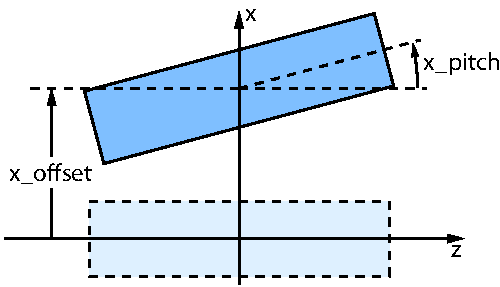
\includegraphics{pitch.pdf}
  \caption{Geometry of Pitch and Offset attributes}
  \label{f:pitch}
\end{figure}

\vn{x_offset} translates an element in the local $x$--direction as shown in
\fig{f:pitch}. Similarly, \vn{y_offset} and \vn{z_offset} translate an element along the local $y$
and $z$--directions respectively.

The \vn{x_pitch} attribute rotates an element about the element's center such that with a positive
\vn{x_pitch} the exit face of the element is displaced in the $+x$--direction as shown in
figure~\ref{f:pitch}. [One way to visualize the effect of an \vn{x_pitch} is to think of the element
as an airplane pointing in the $+z$ direction. A positive \vn{x_pitch} would then move the front of
the plane in the $+x$--direction.] An\vn{x_pitch} represents a rotation around the positive
$y$-axis.

Similarly, the \vn{y_pitch} attribute rotates an element about the element's center using the
negative $x$--axis as the rotation axis so that, with a positive \vn{y_pitch} the exit face of the
element is displaced in the $+y$--direction.

Note: the \vn{x_pitch} and \vn{y_pitch} rotations are about the center of the element which is in contrast
to the \vn{dtheta} and \vn{dphi} misalignments of \mad which rotate around the entrance point. The
sense of the rotation between \bmad and MAD is:
\index{MAD!element rotation origin}
\begin{example}
  x_pitch (Bmad) =  dtheta (MAD)
  y_pitch (Bmad) = -dphi (MAD)
\end{example}

\begin{figure}[tb]
  \centering
  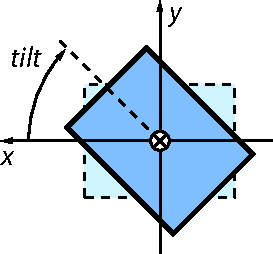
\includegraphics{tilt.pdf}
  \caption{Geometry of a Tilt}
  \label{f:tilt}
\end{figure}

The tilt attribute rotates the element in the $(x, y)$ plane as shown in figure~\ref{f:tilt}. The
rotation axis is the positive $z$-axis. For example
\begin{example}
  q1: quad, l = 0.6, x_offset = 0.03, y_pitch = 0.001, tilt
\end{example}
\index{sol_quad!tilt default}\index{quadrupole!tilt default}
\index{sextupole!tilt default}\index{octupole!tilt default}
Like MAD, \bmad allows the use of the \vn{tilt} attribute without a value to designate a skew
element. The default tilt is $\pi/(2(n+1))$ where $n$ is the order of the element:
\begin{example}
  sol_quad       n = 1
  quadrupole     n = 1
  sextupole      n = 2
  octupole       n = 3
\end{example}

Note that \vn{hkick} and \vn{vkick} attributes are not affected by \vn{tilt} except for \vn{kicker}
and \vn{elseparator} elements.

%-----------------------------------------------------------------
\subsection{Bend Element Orientation}
\label{s:bend.orient}

\begin{figure}[ht]
  \centering
  \includegraphics{roll.pdf}
  \caption[Geometry of a Bend]{
Geometry of a Bend. Like straight line elements, offsets and pitches are calculated with respect to
the coordinates at the center of the bend. The exception is the \vn{roll} attribute which is a
rotation around the axis passing through the entrance and exit points.  Shown here is the geometry
for a bend with \vn{ref_tilt} = 0. That is, the bend is in the $x-z$ plane.}
  \label{f:roll}
\end{figure}

The orientation attributes for \vn{sbend}, \vn{rbend} and \vn{rf_bend} elements is
\begin{example}
  x_offset = <Real>
  y_offset = <Real>
  z_offset = <Real>
  x_pitch  = <Real>
  y_pitch  = <Real>
  ref_tilt = <Real>    ! Shifts and reference orbit rotation axis.
  roll     = <Real>    
\end{example}
The geometry for orienting a bend is shown in \fig{f:roll}. Like straight line elements, the offset
and pitch attributes are evaluated with respect to the center of the element.

Unlike the straight line elements, bends do not have a \vn{tilt} attribute. Rather they have a
\vn{ref_tilt} and a \vn{roll} attribute.  The \vn{roll} attribute rotates the bend along an axis
that runs through the entrance point and exit point as shown in figure~\ref{f:roll}. A \vn{roll}
attribute, like the offset and pitch attributes does not affect the reference orbit.  The major
effect of a \vn{roll} is to give a vertical kick to the beam. For a bend with positive bend angle, a
positive \vn{roll} will move the outside portion ($+x$ side) of the bend upward and the inside
portion (-$x$ side) downward. Much like car racetracks which are typically slanted towards the
inside of a turn.

The \vn{ref_tilt} attribute of a bend rotates the bend about the $z$ axis at the upstream end of the
bend as shown in \fig{f:roll}. Unlike \vn{rolls} and \vn{tilts}, \vn{ref_tilt} also shifts the
rotation axis of the reference orbit along with the physical element. A \vn{bend} with a
\vn{ref_tilt} of $\pi/2$ will bend a beam vertically downward (\sref{s:global}). Note that the
\vn{ref_tilt} attribute of \bmad is the same as the MAD \vn{tilt} attribute.

Important! Do not use \vn{ref_tilt} when doing misalignment studies for a machine. Trying to misalign
a dipole by setting \vn{ref_tilt} will affect the positions of all downstream elements! Rather, use the
\vn{roll} parameter.

%-----------------------------------------------------------------
\subsection{Photon Reflecting Element Orientation}
\label{s:photon.orient}

\begin{figure}[ht]
  \centering
  \includegraphics{reflect-orient.pdf}
  \caption[Geometry of a photon reflecting element orientation]{
Geometry of a photon reflecting element orientation.  The reference coordinates used for defining
the orientational attribute is the entrance reference coordinates.  }
  \label{f:reflect.orient}
\end{figure}

Photon reflecting elements have the following orientational attributes:
\begin{example}
  x_offset = <Real>
  y_offset = <Real>
  z_offset = <Real>
  x_pitch  = <Real>
  y_pitch  = <Real>
  ref_tilt = <Real>    ! Shifts both element and reference orbit.
  tilt     = <Real>    
\end{example}
Roughly, these elements can be viewed as zero length bends except, since there is no center
position, the orientational attributes are defined with respect to the entrance coordinates as shown
in \fig{f:reflect.orient}. Like bend elements, the \vn{ref_tilt} attribute rotates both the physical
element and the reference coordinates.  The \vn{tilt} attribute rotates just the physical
element. Thus the total rotation of the physical element about the entrance $z$ axis is the sum
\vn{tilt} + \vn{ref_tilt}.

Frequently, it is desired to orient reflecting elements with respect to the element's surface. This
can be done using a \vn{girder} element (\sref{s:girder}) which supports the reflecting element and
with the \vn{girder}'s \vn{origin_ele_ref_pt} attribute set to \vn{center}.

%-----------------------------------------------------------------
\subsection{Reference Orbit Manipulator Element Orientation}
\label{s:manip.orient}

The \vn{fork}, \vn{photon_fork}, \vn{floor_shift}, and \vn{patch} elements use the following
attributes to orient their exit edge with respect to their entrance edge:
\begin{example}
  x_offset = <Real>
  y_offset = <Real>
  z_offset = <Real>
  x_pitch  = <Real>
  y_pitch  = <Real>
  tilt     = <Real>    
\end{example}
Here "exit" edge for \vn{fork} and \vn{photon_fork} elements is defined to be the start of the line
being branched to. [Within the line containing the fork, the \vn{fork} element is considered to have
zero length so the exit face in the line containing the fork is coincident with the entrance face.]
The placement of the exit edge for these elements defines the reference orbit.  Thus, unlike the
corresponding attributes for other elements, the orientational attributes here directly control the
reference orbit.

%-----------------------------------------------------------------
\subsection{Fiducial Element Orientation}
\label{s:fiducial.orient}

The \vn{fiducial} element (\sref{s:girder}) uses the 
following attributes to define its position:
\begin{example}
  origin_ele        = <Name>     ! Reference element.
  origin_ele_ref_pt = <location> ! Reference pt on reference ele.
  dx_origin         = <Real>     ! x-position offset
  dy_origin         = <Real>     ! y-position offset
  dz_origin         = <Real>     ! z-position offset
  dtheta_origin     = <Real>     ! orientation angle offset.
  dphi_origin       = <Real>     ! orientation angle offset.
  dpsi_origin       = <Real>     ! orientation angle offset.
\end{example}
See Section~\sref{s:fiducial} for more details.

%-----------------------------------------------------------------
\subsection{Girder Orientation}
\label{s:girder.orient}

A \vn{girder} (\sref{s:girder}) element uses the same attributes as a \vn{fiducial} element
(\sref{s:fiducial}) to orient the reference girder position. In addition, the following attributes
are used to move the girder physically from the reference position:
\begin{example}
  x_offset = <Real>
  y_offset = <Real>
  z_offset = <Real>
  x_pitch  = <Real>
  y_pitch  = <Real>
  tilt     = <Real>    
\end{example}
Shifting the girder from its reference position shifts all the elements that are supported by the
girder. See Section~\sref{s:girder} for more details.

\index{x_offset_tot|hyperbf}\index{y_offset_tot|hyperbf}\index{z_offset_tot|hyperbf}
\index{x_pitch_tot|hyperbf}\index{y_pitch_tot|hyperbf}
\index{tilt_tot|hyperbf}\index{roll_tot|hyperbf}\index{tilt_err_tot|hyperbf}
If an element is supported by a \vn{girder} element (\sref{s:girder}), the orientational attributes
of the element are with respect to the orientation of the \vn{girder}. The computed offsets, pitches
and tilt with respect to the local reference coordinates are stored in the dependent attributes
\begin{example}
  x_offset_tot
  y_offset_tot
  z_offset_tot
  x_pitch_tot
  y_pitch_tot
  tilt_tot
  roll_tot
\end{example}
\index{sbend}\index{rbend}
A \vn{*_tot} attribute will only be present if the corresponding non \vn{*_tot} attribute is
present. For example, only \vn{sbend} and \vn{rbend} elements have a \vn{roll_tot} attribute since
only these elements have a \vn{roll} attribute.

If an element is not supported by a \vn{girder}, the values of the \vn{*_tot} attributes will be the
same value as the values of the corresponding non \vn{*_tot} attributes.

%-----------------------------------------------------------------
\section{Hkick, Vkick, and Kick Attributes}
\label{s:kick}
\index{hkick|hyperbf}\index{bl_hkick|hyperbf}
\index{vkick|hyperbf}\index{bl_vkick|hyperbf}
\index{kick|hyperbf}\index{bl_kick|hyperbf}


\index{hkicker}
\index{vkicker}
\index{elseparator}
\index{kicker}
The kick attributes that an element may have are:
\begin{example}
  kick,  bl_kick  = <Real>  ! Used only with a Hkicker or Vkicker
  hkick, bl_hkick = <Real>
  vkick, bl_vkick = <Real>
\end{example}
\vn{kick}, \vn{hkick}, and \vn{vkick} attributes are the integrated kick of an element in
radians. \vn{kick} is only used for \vn{hkicker} and \vn{vkicker} elements. All other elements that
can kick use \vn{hkick} and \vn{vkick}. The \vn{tilt} attribute will only rotate a kick for
\vn{hkicker}, \vn{vkicker}, \vn{elseparator} and \vn{kicker} elements. This rule was implemented so
that, for example, the \vn{hkick} attribute for a skew quadrupole would represent a horizontal
steering. The \vn{bl_kick}, \vn{bl_hkick}, and \vn{bl_vkick} attributes are the integrated field
kick in \vn{meters-Tesla}. Normally these are dependent attributes except if they appear in the
lattice file (\sref{s:depend}).

For an \vn{elseparator} element, the \vn{hkick} and \vn{vkick} are appropriate for a positively
charged particle. The kick for a negatively charged particle is opposite this.

%-----------------------------------------------------------------
\section{Aperture and Limit Attributes}
\label{s:limit}
\index{aperture|hyperbf}
\index{limit|hyperbf}
\index{aperture_at|hyperbf}

\begin{figure}[ht]
  \centering
  \includegraphics{apertures.pdf}
  \caption[Apertures for ecollimator and rcollimator elements.]
  {Apertures for ecollimator and rcollimator elements. 
  [note: positive $z$ points up, out of the page.] 
  As drawn, all limits \vn{x1_limit}, \vn{x2_limit}, 
  \vn{y1_limit}, \vn{y2_limit} are  positive.}  
  \label{f:limit}
\end{figure}

\index{ecollimator}
\index{rcollimator}
\index{x_limit|hyperbf}
\index{y_limit|hyperbf}
\index{x1_limit|hyperbf}
\index{y1_limit|hyperbf}
\index{x2_limit|hyperbf}
\index{y2_limit|hyperbf}
\index{x_offset|hyperbf}
\index{offset_moves_aperture|hyperbf}
\index{aperture_type}
The aperture attributes are:
\begin{example}
  x1_limit      = <Real>      ! Horizontal, negative side, aperture limit
  x2_limit      = <Real>      ! Horizontal, positive side, aperture limit
  y1_limit      = <Real>      ! Vertical, negative side, aperture limit
  y2_limit      = <Real>      ! Vertical, positive side, aperture limit
  x_limit       = <Real>      ! Alternative to specifying x1_limit and x2_limit
  y_limit       = <Real>      ! Alternative to specifying y1_limit and y2_limit
  aperture      = <Real>      ! Alternative to specifying x_limit and y_limit
  aperture_at   = <Switch>    ! What end aperture is at. (\sref{s:ap.place})
  aperture_type = <Switch>    ! What type of aperture it is
  offset_moves_aperture = <Logical> ! Element offsets affect aperture position (\sref{s:offset.ap})
\end{example}
\vn{x1_limit}, \vn{x2_limit}, \vn{y1_limit}, and \vn{y2_limit} specify the half--width of the
aperture of an element as shown in figure~\ref{f:limit}. Note: Normally all of these will be zero or
positive. A zero \vn{x1_limit}, \vn{x2_limit}, \vn{y1_limit}, or \vn{y2_limit} is interpreted as no
aperture in the appropriate plane.

For convenience, \vn{x_limit} can be used to set \vn{x1_limit} and
\vn{x2_limit} to a common value. Example:
\begin{example}
  s: sextupole, x1_limit = 0.09, x2_limit = 0.09
  s: sextupole, x_limit = 0.09   ! Same as above
\end{example}
Similarly, \vn{y_limit} can be used
to set \vn{y1_limit} and \vn{y2_limit}.  The \vn{aperture} attribute
can be use to set all four \vn{x1_limit}, \vn{x2_limit}, \vn{y1_limit}
and \vn{y2_limit} to a common value. Internally, the \bmad code does {\em not}
store \vn{x_limit}, \vn{y_limit}, or \vn{aperture}. This means that
using \vn{x_limit}, \vn{y_limit} or aperture in arithmetic expressions is
an error:
\begin{example}
  q1: quad, aperture = 0.09         
  q2: quad, aperture = q1[aperture]   ! THIS IS AN ERROR!
  q2: quad, aperture = q1[x1_limit]   ! Correct
\end{example}

By default, apertures are assumed to be rectangular except that an \vn{ecollimator} has a elliptical
aperture. This can be changed by setting the \vn{aperture_type} attribute. The possible values of
this attribute are:
\begin{example}
  auto         ! Default for detector, mask and diffraction_plate elements
  custom
  elliptical   ! Default for \vn{ecollimator} elements.
  rectangular  ! Default for most elements.
  wall3d       ! Vacuum chamber wall (\sref{s:wall}).
\end{example}
The \vn{custom} setting is used in the case where programs have been compiled with custom, non-Bmad,
code to handle the aperture calculation.  The \vn{auto} setting is used for automatic calculation of
a rectangular aperture. For \vn{diffraction_plate} and \vn{mask} elements, the \vn{auto} setting
causes the four aperture limits to be set to just cover the clear area of element
(\sref{s:masking.wall}). For all other elements, the \vn{auto} setting is only to be used when there
is an associated surface grid (\sref{s:surf.grid}) for the element and, in this case, \bmad to set
the four limits to just cover the surface grid.

The \vn{wall3d} setting uses the vacuum chamber wall as specified by a \vn{wall} attribute
(\sref{s:wall}). Using the \vn{wall} construct allows for complex apertures to be
constructed. Note that The wall thickness and material type are not used when calculating
if a particle has hit the wall. That is, the wall is considered to be infinitely thin.
Also note that a wall must cover the entire length of the element longitudinally. This is done
in order to be able to spot errors in specifying the wall geometry.

For elliptical apertures, all four \vn{x1_limit}, \vn{x2_limit}, \vn{y1_limit}, and \vn{y2_limit}
must be non-zero.

For rectangular apertures, the limits \vn{x1_limit}, \vn{x2_limit}, \vn{y1_limit}, or \vn{y2_limit}
may be negative. For example:
\begin{example}
  s: sextupole, x1_limit = -0.02, x2_limit = 0.09
\end{example}
In this case, particles will hit the aperture if their $x$-coordinate is outside the interval [0.02,
0.09]. That is, particles at the origin will be lost.

To avoid numerical overflow and other errors in tracking, a particle will be considered to have hit
an aperture in an element, even if there are no apertures set for that element, if its orbit exceeds
1000 meters. Additionally, there are other situations where a particle will be considered lost. For
example, if a particle's trajectory does not intersect the output face in a bend.

Examples:
\begin{example}
  q1, quadrupole, y1_limit = 0.03
  q1[y2_limit] = 0.03
  q1[y_limit] = 0.03  ! equivalent to the proceeding 2 lines.  
  q1[aperture_at] = both_ends
\end{example}

%-----------------------------------------------------------------
\subsection{Apertures and Element Offsets}
\label{s:offset.ap}

\index{tilt}
\index{x_offset}
\index{y_offset}
\index{x_pitch}
\index{y_pitch}
\index{rcollimator}\index{ecollimator}
\index{multilayer_mirror}\index{mirror}\index{crystal}
Normally, whether a particle hits an aperture or not is evaluated independent of any element offsets
(\sref{s:offset}). This is equivalent to the situation where a beam pipe containing an aperture is
independent of the placement of the physical element the beam pipe passes through. That is, the beam
pipe does not ``touch'' the physical element. This can be changed by setting the
\vn{offset_moves_aperture} attribute to \vn{True}. In this case any offsets or pitches will be
considered to have shifted the aperture boundary. The exceptions here is that the default for the
following elements is for \vn{offset_moves_aperture} to be \vn{True}:
\begin{example}
  rcollimator, 
  ecollimator,
  multilayer_mirror, 
  mirror, and 
  crystal 
\end{example}

Even with \vn{offset_moves_aperture} set to \vn{True}, \vn{tilt}s will not affect the aperture
calculation. This is done, for example, so that the tilt of a skew quadrupole does not affect the
aperture. The exception here is that tilting an \vn{rcollimator} or \vn{ecollimator} element will
tilt the aperture. Additionally, when the aperture is at the \vn{surface} (see below), any \vn{tilt}
will be used in the calculation.

Example:
\begin{example}
  q1: quad, l = 0.6, x1_limit = 0.045, offset_moves_aperture = T
\end{example}

%-----------------------------------------------------------------
\subsection{Aperture Placement}
\label{s:ap.place}

\index{both_ends|hyperbf}\index{continuous|hyperbf}
\index{entrance_end|hyperbf}\index{exit_end|hyperbf}\index{wall_transition|hyperbf}
\index{surface|hyperbf}\index{aperture_at}\index{no_aperture}
By default, for most elements, the aperture is evaluated at the exit face of the element. This can
be changed by setting the \vn{aperture_at} attribute.  Possible settings for \vn{aperture_at} are:
\begin{example}
  both_ends
  continuous
  entrance_end
  exit_end       ! Default for most elements
  no_aperture
  surface  
  wall_transition
\end{example}
The \vn{exit_end} setting is the default for most elements except for
the following elements who have a default of \vn{surface}:
\index{mirror}\index{multilayer_mirror}\index{crystal}
\index{diffraction_plate}\index{sample}
\begin{example}
  crystal
  detector
  diffraction_plate
  mask
  mirror
  multilayer_mirror
  sample
\end{example}

In fact, for the following elements:
\begin{example}
  mirror, 
  multilayer_mirror
  crystal
\end{example}
The \vn{surface} setting for \vn{aperture_at} must be used.  Additionally, due to the complicated
geometry of these elements, to keep things conceptionally simple, the rule is imposed that, for an
aperture at the surface, the \vn{offset_moves_aperture} setting must be left in its default state of
True. Additionally, For \vn{entrance_end} or \vn{exit_end} apertures, \vn{offset_moves_aperture}
must be set to False.

Note: The entrance and exit ends of an element are independent of which direction particles are
tracked through an element. Thus if a particle is tracked backwards it enters an element at the
``exit end'' and exits at the ``entrance end''. The \vn{continuous} setting indicates that the
aperture is continuous along the length of the element. This only matters when particle tracking
involves stepping through an element a little bit at a time. For example, as in Runge-Kutta tracking
(\sref{s:tkm}). For tracking where a formula is used to transform the particle coordinates at the
entrance of an element to the coordinates at the exit end, the aperture is only checked at the end
points so, in this situation, a \vn{continuous} aperture is equivalent to the \vn{both_ends}
setting.

The \vn{wall_transition} setting is like the \vn{continuous} setting in that the aperture boundary
is considered to be continuous along the element's length. However, unlike the \vn{continuous}
setting, with the \vn{wall_transition} setting a particle outside the wall is considered alive and
it is only when a particle moves through the wall that it is lost.  The \vn{wall_transition} setting
is used for things like septum magnets where a particle may be safely outside or inside the
wall. Note to programmers: By supplying a custom \vn{wall_hit_handler_custom} routine, scattering of
particles through a wall may be simulated.

Examples:
\begin{example}
  q2: quad, aperture_type = elliptical, aperture_at = continuous
  q1: quad, l = 0.6, x1_limit = 0.045, offset_moves_aperture = T
\end{example}

%-----------------------------------------------------------------
\subsection{Apertures and X-Ray Generation}
\label{s:aper.x.ray}

With X-ray simulation apertures can be used by \bmad to limit the directions in which photons are
generated. This can greatly decrease simulation times. For example, a photon passing through a
\vn{diffraction_plate} element will diffract in an arbitrary direction. If a {\em downstream}
element has an aperture set, \bmad can restrict the velocity directions so that the photons will
fill the downstream aperture and the amount of time wasted tracking photons that ultimately would be
collimated is minimal.

%-----------------------------------------------------------------
\section{X-Rays Crystal \& Compound Materials}
\label{s:cryst.list}

For basic crystallographic and X-ray matter interaction cross-sections, \bmad uses the
XRAYLIB\cite{b:xraylib} library. Crystal structure parameters in XRAYLIB are mainly from
R.~W.~G.~Wyckoff\cite{b:wyckoff} with some structure parameters coming from NIST. The list of
available structures is:
\begin{center}
\begin{tabular}{llll} \toprule
AlphaAlumina & GaP       & KCl        & Platinum  \\
AlphaQuartz  & GaSb      & KTP        & RbAP      \\
Aluminum     & Ge        & LaB6       & Sapphire  \\
Be           & Gold      & LaB6_NIST  & Si        \\
Beryl        & Graphite  & LiF        & Si_NIST   \\
Copper       & InAs      & LiNbO3     & Si2       \\
CsCl         & InP       & Muscovite  & SiC       \\
CsF          & InSb      & NaCl       & Titanium  \\
Diamond      & Iron      & PET        & TlAP      \\
GaAs         & KAP       &            &           \\ \bottomrule
\end{tabular}
\end{center}
These names are case sensitive

Besides the above crystal list, \bmad can calculate structure factors for all the elements and the
following list of materials. Material properties are from NIST. These names are case sensitive. That
is, the NIST materials all use upper case. As noted in the table, several of the materials may be
specified using the appropriate chemical formula. For example, liquid water may be referenced using
the name \vn{H2O}.
\begin{center}
\footnotesize
\begin{longtable}{lll}
\multicolumn{3}{r}{{\normalsize Continued on next page}} \\
\endfoot
\endlastfoot
A_150_TISSUE_EQUIVALENT_PLASTIC     & LITHIUM_TETRABORATE                       \\
ACETONE                             & LUNG_ICRP                                 \\
ACETYLENE                           & M3_WAX                                    \\
ADENINE                             & MAGNESIUM_CARBONATE                       \\
ADIPOSE_TISSUE_ICRP                 & MAGNESIUM_FLUORIDE                        \\
AIR_DRY_NEAR_SEA_LEVEL              & MAGNESIUM_OXIDE                           \\
ALANINE                             & MAGNESIUM_TETRABORATE                     \\
ALUMINUM_OXIDE, Al2O3               & MERCURIC_IODIDE                           \\
AMBER                               & METHANE                                   \\
AMMONIA, NH3                        & METHANOL                                  \\
ANILINE                             & MIX_D_WAX                                 \\
ANTHRACENE                          & MS20_TISSUE_SUBSTITUTE                    \\
B_100_BONE_EQUIVALENT_PLASTIC       & MUSCLE_SKELETAL                           \\
BAKELITE                            & MUSCLE_STRIATED                           \\
BARIUM_FLUORIDE                     & MUSCLE_EQUIVALENT_LIQUID_WITH_SUCROSE     \\
BARIUM_SULFATE                      & MUSCLE_EQUIVALENT_LIQUID_WITHOUT_SUCROSE  \\
BENZENE, C6H6                       & NAPHTHALENE                               \\
BERYLLIUM_OXIDE                     & NITROBENZENE                              \\
BISMUTH_GERMANIUM_OXIDE             & NITROUS_OXIDE                             \\
BLOOD_ICRP                          & NYLON_DU_PONT_ELVAMIDE_8062               \\
BONE_COMPACT_ICRU                   & NYLON_TYPE_6_AND_TYPE_6_6                 \\
BONE_CORTICAL_ICRP                  & NYLON_TYPE_6_10                           \\
BORON_CARBIDE, B4C                  & NYLON_TYPE_11_RILSAN                      \\
BORON_OXIDE, B2O3                   & OCTANE_LIQUID                             \\
BRAIN_ICRP                          & PARAFFIN_WAX                              \\
BUTANE                              & N_PENTANE                                 \\
N_BUTYL_ALCOHOL                     & PHOTOGRAPHIC_EMULSION                     \\
C_552_AIR_EQUIVALENT_PLASTIC        & PLASTIC_SCINTILLATOR_VINYLTOLUENE_BASED   \\
CADMIUM_TELLURIDE                   & PLUTONIUM_DIOXIDE                         \\
CADMIUM_TUNGSTATE                   & POLYACRYLONITRILE                         \\
CALCIUM_CARBONATE                   & POLYCARBONATE_MAKROLON_LEXAN              \\
CALCIUM_FLUORIDE                    & POLYCHLOROSTYRENE                         \\
CALCIUM_OXIDE                       & POLYETHYLENE                              \\
CALCIUM_SULFATE                     & POLYETHYLENE_TEREPHTHALATE_MYLAR          \\
CALCIUM_TUNGSTATE                   & POLYMETHYL_METHACRALATE_LUCITE_PERSPEX    \\
CARBON_DIOXIDE                      & POLYOXYMETHYLENE                          \\
CARBON_TETRACHLORIDE                & POLYPROPYLENE                             \\
CELLULOSE_ACETATE_CELLOPHANE        & POLYSTYRENE                               \\
CELLULOSE_ACETATE_BUTYRATE          & POLYTETRAFLUOROETHYLENE_TEFLON            \\
CELLULOSE_NITRATE                   & POLYTRIFLUOROCHLOROETHYLENE               \\
CERIC_SULFATE_DOSIMETER_SOLUTION    & POLYVINYL_ACETATE                         \\
CESIUM_FLUORIDE                     & POLYVINYL_ALCOHOL                         \\
CESIUM_IODIDE                       & POLYVINYL_BUTYRAL                         \\
CHLOROBENZENE                       & POLYVINYL_CHLORIDE                        \\
CHLOROFORM                          & POLYVINYLIDENE_CHLORIDE_SARAN             \\
CONCRETE_PORTLAND                   & POLYVINYLIDENE_FLUORIDE                   \\
CYCLOHEXANE                         & POLYVINYL_PYRROLIDONE                     \\
12_DDIHLOROBENZENE                  & POTASSIUM_IODIDE                          \\
DICHLORODIETHYL_ETHER               & POTASSIUM_OXIDE                           \\
12_DICHLOROETHANE                   & PROPANE                                   \\
DIETHYL_ETHER                       & PROPANE_LIQUID                            \\
NN_DIMETHYL_FORMAMIDE               & N_PROPYL_ALCOHOL                          \\
DIMETHYL_SULFOXIDE                  & PYRIDINE                                  \\
ETHANE                              & RUBBER_BUTYL                              \\
ETHYL_ALCOHOL                       & RUBBER_NATURAL                            \\
ETHYL_CELLULOSE                     & RUBBER_NEOPRENE                           \\
ETHYLENE                            & SILICON_DIOXIDE                           \\
EYE_LENS_ICRP                       & SILVER_BROMIDE                            \\
FERRIC_OXIDE                        & SILVER_CHLORIDE                           \\
FERROBORIDE                         & SILVER_HALIDES_IN_PHOTOGRAPHIC_EMULSION   \\
FERROUS_OXIDE                       & SILVER_IODIDE                             \\
FERROUS_SULFATE_DOSIMETER_SOLUTION  & SKIN_ICRP                                 \\
FREON_12                            & SODIUM_CARBONATE                          \\
FREON_12B2                          & SODIUM_IODIDE                             \\
FREON_13                            & SODIUM_MONOXIDE                           \\
FREON_13B1                          & SODIUM_NITRATE                            \\
FREON_13I1                          & STILBENE                                  \\
GADOLINIUM_OXYSULFIDE               & SUCROSE                                   \\
GALLIUM_ARSENIDE                    & TERPHENYL                                 \\
GEL_IN_PHOTOGRAPHIC_EMULSION        & TESTES_ICRP                               \\
GLASS_PYREX                         & TETRACHLOROETHYLENE                       \\
GLASS_LEAD                          & THALLIUM_CHLORIDE                         \\
GLASS_PLATE                         & TISSUE_SOFT_ICRP                          \\
GLUCOSE                             & TISSUE_SOFT_ICRU_FOUR_COMPONENT           \\
GLUTAMINE                           & TISSUE_EQUIVALENT_GAS_METHANE_BASED       \\
GLYCEROL                            & TISSUE_EQUIVALENT_GAS_PROPANE_BASED       \\
GUANINE                             & TITANIUM_DIOXIDE                          \\
GYPSUM_PLASTER_OF_PARIS             & TOLUENE                                   \\
N_HEPTANE                           & TRICHLOROETHYLENE                         \\
N_HEXANE                            & TRIETHYL_PHOSPHATE                        \\
KAPTON_POLYIMIDE_FILM               & TUNGSTEN_HEXAFLUORIDE                     \\
LANTHANUM_OXYBROMIDE                & URANIUM_DICARBIDE                         \\
LANTHANUM_OXYSULFIDE                & URANIUM_MONOCARBIDE                       \\
LEAD_OXIDE                          & URANIUM_OXIDE                             \\
LITHIUM_AMIDE                       & UREA                                      \\
LITHIUM_CARBONATE                   & VALINE                                    \\
LITHIUM_FLUORIDE                    & VITON_FLUOROELASTOMER                     \\
LITHIUM_HYDRIDE                     & WATER_LIQUID, H2O                         \\
LITHIUM_IODIDE                      & WATER_VAPOR                               \\
LITHIUM_OXIDE                       & XYLENE                                    \\
\end{longtable}
\end{center}

%-----------------------------------------------------------------

\begin{figure}[tb]
  \centering
  \includegraphics[width=5in]{surface-curvature.pdf}
  \caption[Surface curvature geometry.]
{Surface curvature geometry. The element reference frame used to describe surface curvature has the
$z$ axis pointing towards the interior of the element, and the $x$ axis in the plane defined by
the entrance and exit reference orbit.}
  \label{f:surface}
\end{figure}

%-----------------------------------------------------------------
\section{X-Ray Reflectivity Tables}
\label{s:reflect}

Reflectivity tables are used to define reflectivity probabilities as functions of incidence angle and
photon energy for \vn{crystal} and \vn{mirror} elements.

The general syntax is:
\begin{example}
  m: mirror, reflectivity_table = \{
    ! A reflection table
    \{
      polarization = <name>
      angles = (<ang1 <ang2 ... <angN>),
      p_reflect = \{
        <energy1> <P_11> <P_12> <P_13> ... <P_1N>,
        <energy2> <P_21> <P_22> <P_23> ... <P_2N>, 
        ...
      \}
    \}
  \}
\end{example}
The \vn{angles} array must be before the \vn{p_reflect} table. Angles are in radians and energy is
in eV. Angle and energy points do not need to be evenly spaced. Probabilities \vn{P_ij} are between
0 and 1. For particles outside the range of angles, the probability is taken to be zero. The
\vn{p_reflect} portion of the reflectivity table must come last.

Possible \vn{polarization} names are:
\begin{example}
  pi        ! Table is for pi mode
  sigma     ! Table is for sigma mode
  both      ! Table is for both polarizations. Default.
\end{example}
An element needs a single table with \vn{polarization} marked as \vn{both} or two tables,
one for \vn{sigma} and the other for \vn{pi}.

For \vn{crystal} elements, angles are always with respect to the Bragg angle for the energy where
the Bragg angle is calculated without any refraction corrections.

%-----------------------------------------------------------------
\section{Surface Properties for X-Ray elements}
\label{s:surface}

The following X-ray elements have a surface which X-rays impinge upon:
\begin{example}
  crystal               \sref{s:crystal}
  detector              \sref{s:detector}
  diffraction_plate     \sref{s:diff.plate}
  mask                  \sref{s:mask}
  mirror, and           \sref{s:mirror}
  multilayer_mirror     \sref{s:multilayer}
  sample                \sref{s:sample}
\end{example}
[There is also the \vn{capillary} element but this element specifies
its surface differently.]

The coordinate system used for characterizing the curvature of a surface is the element reference
frame as shown in \fig{f:surface}). This coordinate system has the $z$ axis pointing towards the
interior of the element, and the $x$ axis in the plane defined by the entrance and exit reference
orbit. In this coordinate system, the surface is an ellipsoid plus a fourth order polynomial in $x$
and $y$ plus a possible ``figure error'' contribution $z_\text{off}$ defined by a surface grid:
\begin{align}
  \label{xs2ij4}
  {-z} &= \frac{1}{g_z} \, \left[ 1 - \sqrt{1 - (g_x \, x)^2 - (g_y \, y)^2} \right] + \\
  &\qquad \qquad \frac{1}{g_{sp}} \, \left[ 1 - \sqrt{1 - (g_{sp} \, x)^2 - (g_{sp} \, y)^2} \right] + 
  \sum_{2 \le i+j \le 6} c_{ij} \, x^i \, y^j - z_\text{off} \nonumber
\end{align}
$z_\text{off}$ is discussed in section~\sref{s:surf.grid} and is only present when the surface grid
\vn{type} is set to \vn{Displacement}. In \Eq{xs2ij4} the $c_{ij}$ coefficients parameterize the
fourth order polynomial, $g_{sp}$ parameterize the spherical curvature, and $g_x, g_y$, and $g_z$
parameterize ellipsoid curvature. [In principle, the spherical curvature is not needed since the
elliptical curvature is more general. In practice, it is sometimes convenient to be able to specify
spherical curvature.]  If $g_z$ is zero, the elliptical curvature is ignored. If $g_z$ or $g_{sp}$
is positive, the curvature is concave towards the incoming photon. If negative, the curvature is
convex. 

The spherical, ellipsoid and polynomial parameters are set for an element by setting the element's
curvature parameter. The syntax is
\begin{example}
  curvature = \{
      spherical    = <Real>,   ! \(g_{sp}\)
      elliptical_x = <Real>,   ! \(g_{x}\)
      elliptical_y = <Real>,   ! \(g_{y}\)
      elliptical_z = <Real>,   ! \(g_{z}\)
      xMyN         = <Real>    ! \(c_{ij}\)
\end{example}

The polynomial coefficients $c_{ij}$ are set via the \vn{xMyN} components where \vn{M} and \vn{N}
are integers in the range 0 through 6 with the restriction
\begin{example}
  2 \(\le\) M + N \(\le\) 6
\end{example}
Example:
\begin{example}
  c2: crystal, curvature = \{spherical = 1/4.7, x2y0 = 0.37, ...\}
\end{example}
in this example, \vn{x2y0} corresponds to the $c_{20}$ term in \Eq{xs2ij4}. To get the
effect of a nonzero $x^0\, y^0$, $x^1 \, y^0$, or $x^0 \, y^1$ terms (since corresponding
\vn{curvature} \vn{xNyM} are not permitted), element offsets and pitches can be used (\sref{s:offset}).

Some useful formulas: Series expansion for a sphere of radius $R$:
\begin{equation}
  {-z} = \frac{x^2}{2 \, R} + \frac{x^4}{8 \, R^3} + \frac{x^6}{16 \, R^5} +
         \frac{y^2}{2 \, R} + \frac{y^4}{8 \, R^3} + \frac{y^6}{16 \, R^5} +
         \frac{x^2 \, y^2}{4 \, R^3} + \frac{3 \, x^4 \, y^2}{16 \, R^5} +
         \frac{3 \, x^2 \, y^4}{16 \, R^5} 
\end{equation}

For a torus with equation
\begin{equation}
  \left( \sqrt{x^2 + (z + r + R)^2} - R \right)^2 + y^2 = r^2
\end{equation}
The series expansion is:
\begin{align}
  {-z} &= \frac{x^2}{2 \, (r+R)} + \frac{x^4}{8 \, (r+R)^3} + \frac{x^6}{16 \, (r+R)^5} + 
         \frac{y^2}{2 \, r} + \frac{y^4}{8 \, r^3} + \\
  & \qquad \frac{y^6}{16 \, r^5} +
         \frac{x^2 \, y^2}{4 \, r \, (r+R)^2} + \frac{3 \, x^4 \, y^2}{16 \, r \, (r + R)^4} + 
         \frac{(3 \, r + R) \, x^2 \, y^4}{16 \, r^3 \, (r + R)^3} \nonumber
\end{align}

For a curved crystal, if $p$ is the distance from the source to the crystal, and $q$ is the distance
from the crystal to the detector, the needed radius of curvature $R_s$ in the sagittal (transverse)
plane to give focusing is \cite{b:del.rio}:
\begin{equation}
  \frac{1}{p} + \frac{1}{q} = \frac{\sin\theta_{g,in} + \sin\theta_{g,out}}{R_s}
\end{equation}
where $\theta_{g,in}$ and $\theta_{g,out}$ are the entrance and exit graze angles. In the tangential
(meridional) plane, the radius $R_t$ needed for focusing is
\begin{equation}
  \frac{\sin^2\theta_{g,in}}{p} + \frac{\sin^2\theta_{g,out}}{q} = \frac{\sin\theta_{g,in} + \sin\theta_{g,out}}{R_t}
\end{equation}
The above formulas assume that the crystal is constructed so that the orientation of the Bragg planes
follows the orientation of the surface. Mirrors have similar formulas with $\theta_{g,in} =
\theta_{g,out} = \theta$.

Example:
\begin{example}
  t_bragg = 1.3950647
  rt = 1  ! Crystal transverse radius
  rs = rt*(sin(t_bragg))^2
  c: crystal, crystal_type =  "Si(553)", b_param = -1, curvature = \{x0y2 = 1 / (2 * rs), 
                      x0y4 = 1 / (8 * rs^3), x2y0 = 1 / (2 * rt), x4y0 = 1 / (8 * rt^3)\}
  c[curvature%x0y2] = 1.01 * c[curvature%x0y2]  ! Put in an error
\end{example}

%-----------------------------------------------------------------
\subsection{Displacement, H_Misalign, and Segmented Surface Grids}
\label{s:surf.grid}
\index{surface grid}

A surface can be broken up into a grid of rectangles. This is useful, for example, in simulating
crystal surface roughness. The case of the \vn{pixel} grid for a \vn{detector} element is discussed
in \Sref{s:detector}. Here the other three types of grids are explained. These are:
\begin{example}
  Displacement       ! Mesh defines an offset from the nominal surface.
  H_Misalign         ! Misalignment of crystal H vector
  Segmented          ! Surface is a matrix of flat rectangles
\end{example}

All grids have the following common parameters:
\begin{example}
  active = <T/F>                     ! Turn on/off effect of grid. Default = True
  ix_bounds = (<ix_min>, <ix_max>),  ! Min/max grid index bounds in x-direction
  iy_bounds = (<iy_min>, <iy_max>),  ! Min/max grid index bounds in y-direction
  r0 = (<x0>, <y0>),                 ! (x,y) coordinates at grid origin
  dr = (<dx>, <dy>),                 ! Spacing between grid points.
\end{example}

Example:
\begin{example}
  ccd: crystal, h_misalign = \{
            r0 = (0.0, 0.01), dr = (0.005, 0.005),
            ix_bounds = (1, 57), iy_bounds = (-30, 10),
            pt(1,-30) = (0.001, -0.002, 0, 0), 
            pt(1,-29) = ..., 
          \}
\end{example}

The grid is a two dimensional rectangular mesh with bounds given by the \vn{ix_bounds} and
\vn{iy_bounds} components. In the above example the grid is 57 pixels in $x$ and 41 pixels in $y$.

The physical placement of the grid on the element is determined by the \vn{r0} and \vn{dr}
components. \vn{r0} is optional and gives the $(x,y)$ coordinates of the center of the pixel with
index $(0,0)$. The \vn{dr} component, which must be present, gives the pixel width and height. Thus
the center of the $(i,j)$ pixel is:
\begin{example}
  (x,y) = (r0(1), r0(2)) + (i*dr(1), j*dr(2))
\end{example}

The different grid types are:
\begin{description}
%
\item[Displacement grid] \Newline
The general syntax for a \vn{displacement} grid is:
\begin{example}
  displacement = \{
      active = <T/F>                     ! Turn on/off effect of grid. Default = True
      ix_bounds = (<ix_min>, <ix_max>),  ! Min/max index bounds in x-direction
      iy_bounds = (<iy_min>, <iy_max>),  ! Min/max index bounds in y-direction
      r0 = (<x0>, <y0>),                 ! (x,y) coordinates at grid origin
      dr = (<dx>, <dy>),                 ! Spacing between grid points.
      pt(<i>,<j>) = (<z>),                                  ! or
      pt(<i>,<j>) = (<z>, <dz/dx>, <dz/dy>),                ! or
      pt(<i>,<j>) = (<z>, <dz/dx>, <dz/dy>, <d2z/dxdy>),
          \}
\end{example}

With a \vn{displacement} grid, an offset $z_\text{off}$ is added to the surface
position defined in \Eq{xs2ij4}. The $z$ offset at a given $(x,y)$ position is determined by a
spline interpolation of the $z$ values of the grid of points defined by \vn{pt(<i>,<j>)}. For each
point \vn{pt(<i>,<j>)}, the $z$ value along with the $dz/dx$, $dz/dy$, $d2z/dxdy$ slopes can be specified or
only the $z$ value needs to be specified. With the later option the slopes will be computed by
taking finite differences of nearest neighbors.
%
\item[H_Misalign grid] \Newline
The general syntax for a \vn{h_misalign} grid:
\begin{example}
  h_misalign = \{
      active = <T/F>                     ! Turn on/off effect of grid. Default = True
      ix_bounds = (<ix_min>, <ix_max>),  ! Min/max index bounds in x-direction
      iy_bounds = (<iy_min>, <iy_max>),  ! Min/max index bounds in y-direction
      r0 = (<x0>, <y0>),                 ! (x,y) coordinates at grid origin
      dr = (<dx>, <dy>)                  ! Spacing between grid points.
      pt(<i>,<j>) = (<rot_y, <rot_x>, <rot_y_rms>, <rot_x_rms>)  ! For Bragg diffraction
      pt(<i>,<j>) = (<rot_y, <rot_z>, <rot_y_rms>, <rot_z_rms>)  ! For Laue diffraction
          \}
\end{example}

An \vn{h_misalign} grid is used with crystals only. With \vn{H_Misalign}, the grid defines
misalignment of the $\bfH$ vector which is the normal to the diffracting planes of the crystal
(\sref{s:crystal.tracking}).  When using \vn{H_Misalign}, each \vn{pt(i,j)} component gives the
angular misalignment of $\bfH$ for the region around the point. for Bragg diffraction where $\bfH$
is oriented approximately along the $-z$-axis, the
misalignment of $\bfH$ is characterized by rotations about the $y$-axis and $x$-axis
\begin{example}
  rot_y_tot = <rot_y> + r2 * <rot_y_rms>
  rot_x_tot = <rot_x> + r1 * <rot_x_rms>
\end{example}
where \vn{rot_x_tot} and \vn{rot_y_tot} are the rotational misalignment (in radians) of $\bfH$
around the $y$-axis and $x$-axis respectively. The small angle approximation is used, That is, it is
assumed that both \vn{rot_x_tot} and \vn{rot_y_tot} are small compared to one. 
the quantities in brackets \vn{<...>} are components of \vn{pt}, and \vn{r1} and
\vn{r2} are Gaussian distributed random numbers with unit rms. These random numbers are regenerated
for each photon.

For Laure diffraction, since the $\bfH$ vector is approximately aligned with the $-x$-axis, the
misalignment is characterized by rotations about the $y$-axis and $z$-axis. Notice that for both
Bragg and Laue diffraction, the rotation around the $y$-axis misaligns (approximately) $\bfH$ in the
plane of the diffraction.
%
\item[Segmented grid] \Newline
The general syntax for a \vn{segmented} grid:
\begin{example}
  segmented = \{
      active = <T/F>                     ! Turn on/off effect of grid. Default = True
      ix_bounds = (<ix_min>, <ix_max>),  ! Min/max index bounds in x-direction
      iy_bounds = (<iy_min>, <iy_max>),  ! Min/max index bounds in y-direction
      r0 = (<x0>, <y0>),                 ! (x,y) coordinates at grid origin
      dr = (<dx>, <dy>)                  ! Spacing between grid points.
          \}
\end{example}

With a \vn{segmented} grid the crystal surface is modeled as a grid of flat ``rectangles'' (the
actual shape is very close but not quite rectangular). Using a segmented surface only makes sense
when the surface is curved (see \Eq{xs2ij4}). There is one rectangle for each grid point. Each rectangle
has an extent in the $(x,y)$ transverse dimensions equal to the spacing between grid points.
\Eq{xs2ij4} is used to calculate the $z$ coordinate of the vertices of a given rectangle and
then these $z$ values are adjusted so that
\begin{example}
  1) The rectangle is flat (the vertices all lie on a plane).
  2) The rectangle contacts the unsegmented surface (\Eq{xs2ij4}) at two diagonally 
       opposite vertices.
  3) The other two diagonally opposite vertices will be as close as possible in the 
       least squares sense from the unsegmented surface.
\end{example}
Note: The \vn{pt} component is not used here.
\end{description}

%-----------------------------------------------------------------
\section{Walls: Vacuum Chamber, Capillary and Mask}
\label{s:wall}
\index{wall}

The \vn{wall} attribute for an element is used to define:
\begin{example}
  vacuum chamber wall
  capillary element (\sref{s:capillary}) inside wall
  diffraction_plate (\sref{s:diff.plate}) geometry
\end{example}

The topics of the following subsections are:
\begin{example}
  \sref{s:wall.syntax}      General wall syntax.
  \sref{s:wall.section}      Cross-section construction. 
  \sref{s:wall.interpolation}      Capillary and vacuum chamber wall interpolation.
  \sref{s:wall.capillary}      Capillary wall.
  \sref{s:wall.vacuum}      Vacuum chamber wall.
  \sref{s:masking.wall}      Diffraction_plate and mask element geometries.
\end{example}

%-----------------------------------------------------------------
\subsection{Wall Syntax}
\label{s:wall.syntax}

The syntax of the \vn{wall} attribute is:
\begin{example}
  wall = \{
    superimpose = <T/F>,               ! Chamber wall only
    thickness = <real>                 ! Default thickness. 
    opaque_material = <material_type>  ! Default opaque material. 
    clear_material = <material_type>   ! Default clear material. 
    section = \{ 
      type = <section_type>,           ! Chamber Mask, and Diffraction_plate only
      s = <longitudinal_position>,     ! Relative to beginning of element.
                                       !   Not used for mask or diffraction_plate.
      r0 = (<x0>, <y0>),               ! section (x,y) origin. Default = (0, 0).
      absolute_vertices = <T/F>,       ! Vertex relative to r0? Default = F.
      material = <material_type>,      ! Mask and Diffraction_plate only.
      thickness = <real>,              ! Mask and Diffraction_plate only.
      dr_ds = <value>,                 ! Capillary and Chamber only
      v(1) = \{<x>, <y>, <radius_x>, <radius_y>, <tilt>\}, 
      v(2) = \{ ... \},
      ...\},
    section = \{
      s = <longitudinal_position>, 
      v(1) = \{... \},
      ... \},
    ... \}
\end{example}
A \vn{wall} begins with ``\vn{wall = \{}'' and ends with a ``\vn{\}}''. In between are a number of
individual cross-section structures. Each individual cross-section begins with ``\vn{section = \{}''
and ends with a ``\vn{\}}''. The \vn{s} parameter of a cross-section gives the longitudinal position
of the cross-section.  Example:
\begin{example}
  this_cap: capillary, 
    wall = \{   
      section = \{ ! cross-section with top/bottom symmetry
        s = 0, v(1) =  \{0.02, 0.00\}, 
        v(2) = \{0.00, 0.02, 0.02\}, v(3) = \{-0.01, 0.01\} \}, 
      section = \{  ! Cross-section that is a tilted ellipse.
        s = 0.34, 
        v(1) = \{0.003, -0.001, 0.015, 0.008, 0.2*pi\} \} \}
\end{example}
In this example an element called \vn{this_cap} is a \vn{capillary}
whose wall is defined by two cross-sections.

%------------------

\begin{figure}[tb]
  \centering
  \includegraphics[width=6in]{chamber-wall.pdf}
  \caption[Capillary or vacuum chamber wall.]
{A) The inside wall of a capillary or the vacuum chamber wall of a non-capillary element is defined
by a number of cross-sectional slices.  B) Each cross-section is made up of a number of
vertices. The segments between the vertices can be either a line segment, the arc of a circle, or a
section of an ellipse.}
  \label{f:chamber.wall}
\end{figure}

%-----------------------------------------------------------------
\subsection{Wall Sections}
\label{s:wall.section}

The wall is defined by a number of cross-sectional slices. For \fig{f:chamber.wall}A shows the
geometry for \vn{capillary} or vacuum chamber walls.  Each cross-section is defined by a
longitudinal position $s$ relative to the beginning of the element and a number of vertices. The arc
between each vertex may be either a straight line, an arc of a circle, or a section of an
ellipse. For a capillary it is mandatory that a cross-section be convex. That is, given any two
points within the cross-section, all points on the line segment connecting them must be within the
cross-section.

The \vn{v(<j>)} within a cross-section define the vertices for each cross-section. The vertices are
defined with respect to the section origin given by \vn{r0}. Each \vn{v(<j>)} has five
parameters. It is mandatory to specify the first two parameters \vn{<x>} and \vn{<y>}. Specifying
the rest, \vn{<radius_x>}, \vn{<radius_y>}, and \vn{<tilt>}, is optional. The default values, if not
specified, is zero. The point (\vn{<x>}, \vn{<y>}) defines the position of the vertex. The
parameters \vn{<radius_x>}, \vn{<radius_y>}, and \vn{<tilt>} define the shape of the segment of the
cross-section between the given vertex and the preceding one.
\begin{example}
  <radius_x>  = 0, <radius_y>  = 0   --> Straight line segment.
  <radius_x> != 0, <radius_y>  = 0   --> Circular arc with radius = radius_x
  <radius_x>  = 0, <radius_y> != 0   --> Illegal!
  <radius_x> != 0, <radius_y> != 0   --> Ellipse section.
\end{example}
When an ellipse is specified, \vn{<radius_x>}, and \vn{<radius_y>} are
the half width and half height of the semi-major axes and the
\vn{<tilt>} parameter gives the tilt of the ellipse. \vn{<radius_x>}
and \vn{<radius_y>} must not be negative.

In the example above, for the first cross-section, \vn{v(2)} specifies a non-zero \vn{<radius_x>}
and, by default, \vn{<radius_y>} is zero. Thus the segment of the cross-section between \vn{v(1)}
and \vn{v(2)} is circular in nature with a radius of 0.02. Since \vn{v(3)} does not specify
\vn{<radius_x>} nor \vn{<radius_y>}, the cross-section between \vn{v(2)} and \vn{v(3)} is a straight
line segment.

The vertex points must be arranged in a ``counter clockwise manner''.  For vertices \vn{<v(i)>} and
\vn{<v(i+1)>} connected by a line segment this translates to
\begin{equation}
  0 < \theta_{i+1} - \theta_{i} \pmod{2\pi} < \pi
  \label{0tt2p}
\end{equation}
where $(r_n, \theta_n)$ are the polar coordinates of the $n^{th}$ vertex with respect to the point
\vn{r0}. For vertices connected by an arc, ``counter clockwise manner'' means that the line segment
with one end at the center of the arc and the other end traversing the arc from \vn{<v(i)>} to
\vn{<v(i+1)>} rotates in counter clockwise as shown in \fig{f:chamber.wall}B.

The red line segment with one end at the center of the arc and the other end traversing the arc
from, in this case, $V(2)$ to $V(3)$, rotates in counter clockwise manner. In general, there are two
solutions for constructing such an arc. For positive radii, the solution chosen is the one whose
center is closest to the section origin $(x_0, y_0)$. If the radii are negative, the center point
will be the point farthest from the origin (the dashed line between $V(2)$ and $V(3)$ in the
figure).

A restriction on cross-sections is that the section origin $(x_0, y_0)$ must be in the interior of
any cross-section and that for any cross-section a line drawn from the origin at any given angle
$\theta$ will intersect the cross-section at exactly one point as shown in
\fig{f:chamber.wall}B. This is an important point in the construction of the wall between
cross-sections as explained below.

The last vertex specified, call it \vn{<v(n)>}, should not have the same \vn{<x>}, \vn{<y>} values
as the first vertex \vn{<v(1)>}. That is, there will be a segment of the cross-section connecting
\vn{<v(n)>} to \vn{<v(1)>}. The geometry of this segment is determined by the parameters of
\vn{<v(1)>}.

If there is mirror symmetry about the $x$ or $y$ axis for a cross-section, the ``mirrored''
vertices, on the ``negative'' side of the mirror plane, do not have to be specified. Thus if all the
vertex points of a cross-section are in the first quadrant, that is, all \vn{<x>} and \vn{<y>} are
zero or positive, mirror symmetry about both the $x$ and $y$ axes is assumed. If all the \vn{<y>}
values are zero or positive and some \vn{<x>} values are positive and some are negative, mirror
symmetry about the $x$ axis is assumed. Finally, if all the \vn{<x>} values are zero or positive but
some \vn{<y>} values are positive and some are negative, symmetry about the $y$ axis is assumed. For
example, for the first in the above example, since all the \vn{<y>} values are non-negative and
there are positive and negative \vn{<x>} values, symmetry about the $x$ axis is assumed.

The one exception to the above rule that (\vn{<x>}, \vn{<y>}) is the vertex center is when a single
vertex \vn{v(1)} is specified for a cross-section with a non-zero \vn{<radius_x>}. In this case,
(\vn{<x>}, \vn{<y>}) are taken to be the center of the circle or ellipse. For example, if a single
vertex is specified for a cross-section as:
\begin{example}
  section = \{s = 0.3, v(1) = \{0.03, -0.01, 0.15, 0.08, 0.2\}\}
\end{example}
the cross-section will be an ellipse with center at $(0.03, -0.01)$ with a tilt of $0.2$ and axes
radii of $0.15$ and $0.08$. If a cross-section has a single vertex and \vn{<radius_x>} is not
specified, the cross-section is a rectangle. For example
\begin{example}
  section = \{s = 0.3, v(1) = \{0.03, 0.01\}\}
\end{example}

The vertices are defined with respect to the local sector origin $r_0$ except if
\vn{absolute_vertices} is set to \vn{True} in which case the vertex numbers are taken as absolute.
For example, the following two cross-sections are identical and describe a rectangle with edges at
$x = 1$ and 5 and $y = -6$ and 6
\begin{example}
  section = \{absolute_vertices = T, r0 = (4, 0), 
                  v(1) = \{5, 6\}, v(2) = \{1, 6\}, v(3) = \{1, -6\}, v(4) = \{5, -6\}\}
  section = \{r0 = (4, 0), v(1) = \{2, 6\}\}
\end{example}
Notice that while $r0$ is not needed in the first section for positioning of the vertices, it is
needed in the first section to make \Eq{0tt2p} true.

%-----------------------------------------------------------------
\subsection{Interpolation Between Sections}
\label{s:wall.interpolation}

\begin{figure}[tb]
  \centering
  \includegraphics[width=4in]{concave-capillary.pdf}
  \caption[Convex cross-sections do not guarantee a convex volume.]
{Example where convex cross-sections do not produce a convex volume.  Cross-sections (A) and (C) are
ellipses with a 5 to 1 aspect ratio.  Half way in between, linear interpolation produces a convex
cross-section as shown in (B).}
  \label{f:concave.capillary}
\end{figure}

For \vn{capillary} and vacuum chamber walls, the wall between cross-sections, is defined by
interpolation. At a given $s$ position, the $r, \theta$ coordinate system in the transverse $x, y$
plane is defined with respect to an origin $\bfr_O(s)$ given by a linear interpolation of the
origins of the cross-sections to either side of the given $s$ position. Let $s_1$ denote the
position of the cross-section just before $s$ and $s_2$ denote the position of the cross-section
just after $s$. Let $\bfr_{01}$ be the $(x_0, y_0)$ origin defined for the cross section at $s_1$
and $\bfr_{02}$ be the $(x_0, y_0)$ origin defined for the cross section at $s_2$. Then
\begin{equation}
  \bfr_O(s) = (1 - \stilde) \, \bfr_{01} + \stilde \, \bfr_{02}
\end{equation}
where 
\begin{equation}
  \stilde \equiv \frac{s - s_1}{s_2 - s_1}
\end{equation}

Let $r_{c1}(\theta)$ and $r_{c2}(\theta)$ be the radius of the wall as a function of $\theta$ for
the cross-sections at $s = s_1$ and $s = s_2$ respectively. The wall $r_c(\theta, s)$ at any point
$s$ between $s_1$ and $s_2$ is then defined by the equation
\begin{equation}
  r_c(\theta, s) = p_1(\stilde) \, r_{c1}(\theta) + p_2(\stilde) \, r_{c2}(\theta)
\end{equation}
where $p_1$ and $p_2$ are cubic polynomials parameterized by
\begin{align}
  p_1 &= 1 - \stilde + a_1 \, \stilde + a_2 \, \stilde^2 + a_3 \, \stilde^3 \CRNO
  p_2 &= \stilde + b_1 \, \stilde + b_2 \, \stilde^2 + b_3 \, \stilde^3 
\end{align}
If $a_i = b_i = 0$ for all $i = 1, 2, 3$, the interpolation is linear and this is the default if
either of the parameters \vn{dr_ds1} and \vn{dr_ds2} are not given in the wall definition. These
parameters are the slopes of the wall with respect to $s$ at the end points
\begin{equation}
  \text{dr_ds1} \equiv \left. \frac{d\overline{r}}{ds} \right|_{s = s_1} \comma \qquad
  \text{dr_ds2} \equiv \left. \frac{d\overline{r}}{ds} \right|_{s = s_2} 
\end{equation}
where $\overline{r}$ is the average $r$ averaged over all $\theta$. When {\em both} \vn{dr_ds1} and
\vn{dr_ds2} are specified, the $a_i$ and $b_i$ are calculated so that the slopes of the wall match
the values of \vn{dr_ds1} and \vn{dr_ds2} along with the constraints.
\begin{align}
  p_1(0) &= 1 \comma \qquad p_1(1) = 0 \CRNO
  p_2(0) &= 0 \comma \qquad p_2(1) = 1 \\
  M &\equiv a_1^2 + a_2^2 + a_3^2 + b_1^2 + b_2^2 + b_3^2 \text{ is a minimum}
  \nonumber
\end{align}
The last constraint ensures a ``smooth'' transition between the two cross-sections.

To refer to a cross-section parameters after an element has been defined, the following syntax is
used:
\begin{example}
  ele_name[wall%section(n)%v(j)%x]   ! x value of j^th vertex of n^th cross-section
\end{example}

%-----------------------------------------------------------------
\subsection{Capillary Wall}
\label{s:wall.capillary}
\index{capillary!wall}

For a \vn{capillary}, \vn{s} must be zero for the first cross-section and the length of the
capillary is given by the value of \vn{s} of the last cross-section.

For a \vn{capillary}, in order for \bmad to quickly track photons, \bmad assumes that the volume
between the cross-sections is convex. The volume will be convex if each cross-section $r_c(\theta,
s)$ at any given $s$ is convex. Note that it is {\em not} sufficient for $r_c(\theta, s)$ to be
convex at the specified cross-sections as shown in \fig{f:concave.capillary}. Also note that it is
perfectly fine for the total capillary volume to not be convex.

%-----------------------------------------------------------------
\subsection{Vacuum Chamber Wall}
\label{s:wall.vacuum}

The vacuum chamber wall is independent of the element apertures (\sref{s:limit}). Unless a program
is specifically constructed, the presence of a vacuum chamber wall will not affect particle
tracking.

The vacuum chamber wall defined for an element may be shorter or longer than the element.  The
vacuum chamber wall for a particular lattice branch is the sum of all the chamber walls of the
individual elements. That is, the chamber wall at any given point is determined by interpolation of
the nearest sections upstream and downstream to the point.  Thus a given lattice element need not
contain a \vn{wall} component for the chamber wall to be well defined at the element.

The exception to the above rule is when a \vn{section} has its
\vn{type} component set to either:
\begin{example}
  wall_start
  wall_end
\end{example}
\vn{wall_start} and \vn{wall_end} sections must come in pairs. The next section after a
\vn{wall_end} section (if this section is not the last section in the lattice) must be a
\vn{wall_start} section.  If a section has a \vn{type} of \vn{wall_start}, the region between that
section and the previous section (which must be a \vn{wall_end} section) will be considered to have
no wall. If the \vn{wall_start} section is the first section of the lattice branch, the region of no
wall will start at the beginning of the branch. Similarly, if a section has a \vn{type} of
\vn{wall_end}, the region between that section and the next section (or the end of the lattice
branch if there is no next section) will not have a wall.

The chamber walls of any two elements may not overlap. The exception is when the \vn{superimpose}
attribute for a wall of an element is set to True. In this case, any other wall cross-sections from
any other elements that overlap the superimposed wall are discarded.  Superposition of a wall is
useful, for example, in introducing mask regions into the wall.

If a branch has a closed geometry (\sref{s:param}), wall sections that extend beyond the ends of the
branch are ``wrapped'' around.

If a particle is past the last wall cross-section or before the first wall cross-section, The
following rules are used: If the branch has a \vn{closed geometry}, the wall will be interpolated
between the last and first cross-sections. If the branch has an \vn{open} geometry, the wall is
taken to have a constant cross-section in these regions.

The chamber wall is defined with respect to the local coordinate system (\sref{s:ref}). That is, in
a bend a wall that has a constant cross section is a section of a torus.

\index{patch!and chamber wall}
\vn{Patch} elements (\sref{s:patch}) complicate the wall geometry since the coordinate system at the
end of the \vn{patch} may be arbitrarily located relative to the beginning of the patch. To avoid
confusion as to what coordinate system a wall section belongs to, \vn{patch} elements are not
allowed to define a wall. The wall through a patch is determined by the closest wall sections of
neighboring elements.

%-------------------

\begin{figure}[tb]
  \centering
  \includegraphics[width=6in]{crotch.pdf}
  \caption[vacuum chamber crotch geometry.]
{A) Crotch geometry: Two pipes labeled ``leg1'' and ``leg2'' merge into a single pipe called the
``trunk'' pipe. Five wall sections are used to define the crotch geometry (solid lines). Dashed
lines represent sections not involved in defining the crotch. For purposes of illustration, the
three trunk sections are displaced longitudinally but in reality must have the same longitudinal
coordinate.  B) Example layout of the trunk1, trunk2 and trunk wall sections. $O_1$, $O_2$ and $O$
are the $x_0, y_0$ origins of the sections.}
  \label{f:crotch}
\end{figure}

%-------------------

\index{crotch chamber geometry}
Each section has a \vn{type} attribute. This attribute is not used for \vn{capillary} elements. For
a vacuum chamber wall, the \vn{type} attribute is used to describe a ``crotch'' geometry where two
pipes merge into one pipe. The possible values for the \vn{type} attribute are:
\begin{example}
  normal     ! default
  leg1
  leg2
  trunk1
  trunk2
  trunk
\end{example}
The geometry of a crotch is shown in \fig{f:crotch}A. Two pipes, called ``leg1'' and ``leg2'', merge
into one pipe called the ``trunk'' pipe.  The trunk pipe can be either upstream or downstream of the
leg pipes.  To describe this situation, five sections are needed: One section in each leg pipe which
need to have their \vn{type} attribute set to \vn{leg1} and \vn{leg2}, and three sections in the
trunk with one having a a \vn{type} attribute of \vn{trunk1}, another having a \vn{type} attribute
of \vn{trunk2} and the third having a \vn{type} attribute of \vn{trunk}. There can be no sections
between the leg sections and the trunk sections.

All three trunk sections must be associated with the same element and have the same \vn{s} value. In
the list of sections of the element containing the trunk elements, the \vn{trunk1} and \vn{trunk2}
sections must be listed first if the leg pipes are upstream of the trunk pipe (the situation shown
in the figure) and must be listed last if the leg pipes are downstream. That is, the \vn{trunk1} and
\vn{trunk2} sections are ``between'' the leg sections and the \vn{trunk} section. It does not matter
if \vn{trunk1} is before or after \vn{trunk2}.

The \vn{trunk1} and \vn{trunk2} sections must not overlap and the \vn{trunk} section must be
constructed so that its area is the union of the areas of \vn{trunk1} and \vn{trunk2}. An example is
illustrated in \fig{f:crotch}B. Here the \vn{trunk1} and \vn{trunk2} sections are squares with
origins labeled $O_1$ and $O_2$ in the figure. By necessity, these origins must be different since
each must lie within the boundaries of their respective areas. The \vn{trunk} section is a rectangle
encompassing the two squares and has an origin labeled $O$.

Between \vn{leg1} and \vn{trunk1} sections the wall is interpolated using these two
section. Similarly for the region between \vn{leg2} and \vn{trunk2} sections. Away from these
regions interpolation is done as outlined in \sref{s:wall.interpolation}. However, these two regions
need a different interpolation scheme since, \vn{leg1} and \vn{trunk1}, as well as \vn{leg2} and
\vn{trunk2} sections do not have to be parallel to each other.

%-----------------------------------------------------------------
\subsection{Mask Wall For Diffraction Plate and Mask Elements}
\label{s:masking.wall}

\begin{figure}[tb]
  \centering
  \includegraphics[width=6in]{diffraction-plate.pdf}
  \caption[Example mask wall]{
A) The surface of a \vn{diffraction_plate} or \vn{mask} element is divided into ``clear'' (white)
and ``opaque'' (black) areas. As explained in the text, these areas are defined by five
\vn{sections} labeled $s_1$ through $s_5$. B) All wall sections must be star shaped with respect to
the section's origin. In this example, The section is {\em not} star shaped since a line drawn from
the origin point $o$ to the point $p$ on the boundary intersects the boundary twice in between. In
this case the section can be made star shaped by moving the origin to $o'$.
  }
  \label{f:diff.plate}
\end{figure}

The \vn{wall} attribute (\sref{s:wall}) of a \vn{diffraction_plate} or \vn{mask} element specifies
what areas of the element will transmit or reflect particle and what areas will not. Here the
``wall'' defines a 2-dimensional area where particles (or X-rays) impinge upon and not a
3-dimensional surface.  As such, the \vn{s} longitudinal position parameter of wall \vn{sections} is
not used with \vn{mask} and \vn{diffraction_plate} elements.

The algorithm used to decide if a particle hitting a given point will be transmitted or not is as
follows.  A \vn{wall} is comprised a a ordered list of \vn{sections} as discussed in
\sref{s:wall.section}.  Sections will be labeled $s_1, s_2, s_3, \ldots$ with $s_i$ being the $i$\Th
section defined in the \vn{wall} structure. Each section of the wall must have its \vn{type}
attribute set to one of:
\begin{example}
  clear
  opaque
\end{example}
A section is called ``clear'' or ``opaque'' depending upon the setting of its \vn{type} attribute.
The first section $s_1$ must be labeled \vn{clear}. Each \vn{clear} section has zero or more
associated \vn{opaque} sections that follow the \vn{clear} section. An opaque section $s_j$ is
associated with clear section $s_i$ if and only if $i$ is less than $j$, and all the sections $k$
between $i$ and $j$ (that is, $i < k < j$) are opaque sections. For example, if the \vn{wall}
defines 6 sections:
\begin{example}
  \(s_1\)   Clear
  \(s_2\)   Clear
  \(s_3\)   Opaque
  \(s_4\)   Opaque
  \(s_5\)   Clear
  \(s_6\)   Opaque
\end{example}
with this arrangement, clear section $s_1$ does not have any associated opaque sections, clear section
$s_2$ has two associated opaque section $s_3$ and $s_4$, and clear section $s_5$ has one associated
opaque section $s_6$.

Each \vn{section} covers an area specified by the vertex list associated with the \vn{section}. To
decide if a particle is transmitted, each clear section, starting from $s_1$, is tested to see if
the particle's $(x,y)$ coordinates is within the section. If the particle position is not within any
clear section, the particle is considered to have hit an opaque region. If a particle is within one
or more clear regions, let $s_i$ be the clear region with the smallest index $i$ that the particle
is within. The particle is transmitted if the particle is outside of all associated opaque region of
$s_i$.

When tracking photons, any clear section can be given a \vn{material} and \vn{thickness}. Available
materials are listed in \sref{s:cryst.list}. A photon transversing a clear area with a defined
material will be attenuated and have a phase shift. Note that \vn{material} and \vn{thickness}
properties are not to be assigned to \vn{opaque} sections.

To enable \bmad to quickly calculate whether a particle has landed on a clear or opaque section, All
sections, both clear and opaque, must be ``star shaped'' with respect to the $(x_0, y_0)$ origin
used by the section. That is, a line drawn from the section origin to any point on the section
boundary must not pass through any boundary points of the section in between. This is illustrated in
\fig{f:diff.plate}B where the section is not star shaped since a line drawn from the origin $o$ to
the point $p$ on the boundary passes through two boundary points in between. In this case the
section can trivially be made star shaped by moving the origin to point $o'$. If it is not possible
to make a section star shaped by moving the origin, the section must be divided into multiple
sections.

An example geometry is shown in \fig{f:diff.plate}A. A wall that constructs this geometry is:
\begin{example}
  z_plate: diffraction_plate, wall = \{
    section = \{          ! \(s_1\) 
      type = clear,
      v(1) = \{0, 0, 0.03, 0.013\},
    section = \{          ! \(s_2\)
      type = opaque,
      v(1) = \{0, 0, 0.005\},
    section = \{          ! \(s_3\)
      type = opaque,
      r0 = (0.02, 0.00),
      v(1) = \{0, 0, 0.005\} \}
    section = \{          ! \(s_4\)
      type = clear, 
      v(1) = \{0.04, 0\}, v(2) = \{0.04, 0.022\},
      v(3) = \{0, 0.03\},
    section = \{          ! \(s_5\)
      type = opaque,
      v(1) = \{0.032, 0.016\},
\end{example}
There are two clear sections $s_1$ and $s_4$. Clear section $s_1$ has an oval shape and has two
associated circular opaque sections $s_2$ and $s_3$. Clear section $s_4$ has a hexagonal shape and
has one associated rectangular opaque section $s_5$. Notice that because opaque section $s_5$ is
associated with clear section $s_4$, and since clear section $s_4$ comes after clear section $s_1$,
opaque section $s_5$ does not affect clear section $s_1$ even though $s_5$ (completely) overlaps
$s_1$. This shows that the ordering of the clear sections is important but the ordering of the
opaque sections associated with a given clear section is not important.

%-----------------------------------------------------------------
\section{Length Attributes}
\label{s:l}

\index{length of elements}
\index{l|hyperbf}
\index{l_chord|hyperbf}
\index{rbend}
\index{sbend}
The length attributes are
\begin{example}
  l           = <Real>  ! 
  l_chord     = <Real>  ! Chord length of a bend. Dependent attribute.
  l_rectangle = <Real>  ! Rectangular length. See \sref{s:bend}
\end{example}
The length \vn{l} is the path length of the reference particle. The one exception is for an
\vn{rbend}, the length \vn{l} set in the lattice file is the chord length
(\sref{s:bend}). internally, \bmad converts all \vn{rbend}s to \vn{sbend}s and stores the chord
length under the \vn{l_chord} attribute.  Example:
\begin{example}
  b: rbend, l = 0.6   ! For rbends, l will be converted to l_chord
\end{example}

\index{girder}
For a \vn{girder} element the length \vn{l} is a dependent attribute and is set by \bmad to be the
difference in longitudinal position $s$ of the downstream end of the last element supported relative
to the upstream end of the first element.

\index{wiggler}
For \vn{wiggler}s, the length \vn{l} is not the same as the path length for a particle with the
reference energy starting on the reference orbit. See~\sref{s:ref}.

\index{patch}
For \vn{patch} elements the \vn{l} length is, by definition, equal to \vn{z_offset}. For \vn{patch}
elements, \vn{l} is a dependent attribute and will be automatically set to \vn{z_offset} by \bmad.

\index{capillary}
The length of a \vn{capillary} element is a dependent variable and is given by the value of \vn{s}
of the last wall cross-section (\sref{s:wall.capillary}).

\index{crystal}
The length of a crystal is zero for Bragg diffraction and is a dependent attribute dependent upon
the crystal thickness for Laue diffraction. See \sref{s:crystal} for more details.

%-----------------------------------------------------------------
\section{Is_on Attribute}
\label{s:is.on}
\index{is_on|hyperbf}

The \vn{is_on} attribute
\begin{example}
  is_on = <Logical>
\end{example}
is used to turn an element off. Turning
an element off essentially converts it into a drift.
Example
\begin{example}
  q1: quad, l = 0.6, k1 = 0.95
  q1[is_on] = False
\end{example}

\index{aperture}
\index{reference orbit}
\index{reference energy}
\vn{is_on} does not affect any apertures that are set. Additionally, \vn{is_on} does not affect the
reference orbit (\sref{s:ref}) or reference energy (\sref{s:ref.energy}). For example, turning off an
\vn{lcavity} will not affect the reference energy.

The following elements cannot be ``turned off:''
\begin{example}
  beginning_ele       null_ele
  capillary           overlay
  crystal             hybrid
  drift               mirror
  fiducial            multilayer_mirror
  floor_shift         photon_init
  patch               sample
  group
\end{example}

A related parameter is \vn{multipoles_on} (\sref{s:multip}).

%-----------------------------------------------------------------
\section{Multipole Attributes: Magnetic and Electric}
\label{s:multip}

Multipole formulas for are given in \sref{s:mag.field} and \sref{s:elec.field}. Note that the
setting of \vn{field_master} (\sref{s:field.master}) will determine if multipoles are interpreted as
normalized or unnormalized.

\index{multipole!knl, tn|hyperbf} 
\index{multipole}
A \vn{multipole} (\sref{s:mult}) element specifies its magnetic multipole components using normal
and skew components with a tilt
\begin{example}
  KnL  = <Real>  ! Normal component. n = Integer. 
  KnSL = <Real>  ! Skew component. n = Integer. 
  Tn   = <Real>  ! Tilt. n = Integer. Default is $pi$/(2n + 2)
\end{example}
Where \vn{n} is an integer in the range from 0 (dipole component) through 21.  If \vn{Tn} is given
without a value, a default of $pi$/(2n + 2) will be used producing a skew field. Example:
\begin{example}
  m: multipole, k1l = 0.32, t1  ! Skew quadrupole of strength 0.32
\end{example}
Following \vn{MAD}, a non-zero dipole (\vn{K0L} component will affect the reference orbit (just like
a normal dipole will). This is not true for any other element.

\index{ab_multipole}
\index{multipole!an, bn|hyperbf} 
An \vn{ab_multipole} (\sref{s:ab.m}) specifies magnetic multipoles
using normal (\vn{Bn}) and skew (\vn{An}) components:
\begin{example}
  An = <Real>
  Bn = <Real>
\end{example}
Here \vn{n} ranges from 0 (dipole component) through 21. Example:
\begin{example}
  q1: ab_multipole, b2 = 0.12, a20 = 1e7, field_master = T
\end{example}
Note that there is a factor of $n$-factorial difference between \vn{An}, \vn{Bn} and \vn{KnL},
\vn{KnSL} multipoles \sref{s:mag.field}.

\index{r0_mag}\index{scale_multipoles}
Elements like \vn{quadrupoles} and \vn{sextupoles} can have assigned to them both magnetic and
electric multipole fields. In this case, the magnetic fields are specified using the same convention
as the \vn{ab_multipole}.  For such non-multipole elements, the magnetic multipole strength is
scaled via (\Eq{ababf}) 
\begin{equation}
a_n(\text{actual}) = F \, \frac{r_0^{n_\REF}}{r_0^n} \, a_n(\text{input}), \qquad
b_n(\text{actual}) = F \, \frac{r_0^{n_\REF}}{r_0^n} \, b_n(\text{input})
\end{equation}
where ``\vn{input}'' denotes the input value set in the lattice file, ``\vn{actual}'' denotes the
value that is used to compute the field, $F$ is the strength of the element (for example $F$ is $K1 \cdot
L$ for a quadrupole), and $r_0$ is the ``measurement radius'' and is set by the \vn{r0_mag}
attribute. The default value of $r_0$ is 0 in which case the factor of $r_0^{n_\REF}/r_0^n$ is
omitted. The scaling may be turned off altogether by setting the \vn{scale_multipoles} attribute.
Example:
\begin{example}
  q1: quadrupole, b2 = 0.12, a20 = 1e7, scale_multipoles = F
\end{example}

Electric multipoles are specified using normal (\vn{Bn_elec}) and skew
(\vn{An_elec}) components. \begin{example}
  An_elec = <Real>
  Bn_elec = <Real>
\end{example}
Here \vn{n} ranges from 0 (dipole component) through 21. Like the magnetic multipoles, a measurement
radius \vn{r0_elec} can be used to scale the multipoles as explained in \sref{s:elec.field}.
Example:
\begin{example}
  q1: quadrupole, l = 1.2, b2_elec = 1e6, r0_elec = 0.034
\end{example}
See \sref{s:elec.field} for how electric multipoles are defined. Notice that Electric multipoles are
never scaled by the element's field strength as they are with magnetic multipoles. If the value of
\vn{r0_elec} is zero (the default) the multipoles will not be scaled.

Unlike magnetic multipoles, there are no factors of the reference momentum nor the element length in
the definition for electric multipoles. That is, electric multipole values represent the field and
not the normalized integrated field. Thus an electric multipole associated with a zero length
element will have no effect on tracking. This being the case, \bmad does not allow electric
multipole values to be specified for \vn{multipole} and \vn{ab_multipole} elements. Indeed, in the
limit of zero element length at constant integrated electric field strength, the equations of motion
are singular since, unlike the magnetic case, the infinite fringe fields give rise to infinite
energy shifts.

\index{multipoles_on}
The magnetic and electric multipole kick can be toggled on or off using the
\vn{multipoles_on} attribute. Example:
\begin{example}
  call, file = "lattice.bmad"             ! Read in a lattice file
  quadrupole::*[multipoles_on] = False    ! But I want the multipoles off.
  q1[k1] = 0.3                            ! k1 attribute not affected.
\end{example}
\vn{multipoles_on} only effect multipoles specified by \vn{An}, \vn{Bn}, \vn{An_elec}, or
\vn{Bn_elec}. Other multipoles, like the \vn{k2} multipole of a \vn{sextupole}, are not
affected. The exception is \vn{multipole} and \vn{ab_multipole} elements do not have the
\vn{multipoles_on} attribute. Rather they can be toggles on/off using the \vn{is_on}
attribute.

%-----------------------------------------------------------------
\section{Field Maps}
\label{s:fieldmap}
\index{field maps}

There are two general ways to specify complicated electro-magnetic field configurations
that cannot be simply modeled using multipoles. One way is to use \vn{custom}
fields. Specifying a custom field is done by using custom code and linking this code with
\bmad into a program. That is, custom fields are defined outside of the \bmad software
(\sref{s:integ}).

\index{cylindrical_map}\index{cartesian_map}\index{grid_field}\index{gen_grad_map}
The other way to specify a complicated field is to use a ``\vn{field map}''. There
are four types of field maps:
\begin{example}
  cartesian_map       ! \sref{s:cart.map}
  cylindrical_map     ! \sref{s:cylind.map}
  grid_field          ! \sref{s:grid.field}
  gen_grad_map        ! \sref{s:gen.grad.map}
\end{example}
Essentially, \vn{cylindrical_map} and \vn{cartesian_map} define fields using a set of
functions with user defined coefficients with the functions formulated to obey Maxwell's
equations. The \vn{grid_field} type defines the field on a grid of points and
interpolation is used to evaluate the field in between the points. Finally, the
\vn{gen_grad_map} type defines a set of ``generalized gradients'' (\sref{s:gen.grad.phys}).

The \vn{cylindrical_map} and \vn{grid_field} types can be used with both RF and DC fields.
The other two types can only be used with DC fields. RF fields may only be used with the following
element classes:
\begin{example}
  e_gun         ! \sref{s:e.gun}
  em_field      ! \sref{s:em.field}
  lcavity       ! \sref{s:lcav}
  rfcavity      ! \sref{s:rfcav}
\end{example}

An element may specify multiple fields of a given type and/or may define multiple fields
of different types. In both these cases, the field in the element is taken to be the sum
of the individual fields. For example:
\begin{example}
  sb: sbend, field_calc = fieldmap, cylindrical_map = \{...\},  cylindrical_map = \{...\}
\end{example}
In this example an element has two \vn{cylindrical_map} fields and the total field is the
sum of the fields of each one. Separating fields like this can be useful, for example, to
decouple the specification of electric from magnetic fields, or to decouple the
specification of AC and DC fields.

The field of one element can overlap onto other elements. This is explained in
Sec.~\sref{s:overlap}.

Field maps are used with integration type tracking methods (\sref{s:integ}).  It is important to
note that field maps are {\em ignored} by \vn{bmad_standard} tracking. Additionally, \vn{grid_field}
field maps cannot be used with \vn{symp_lie_ptc}.

Field maps may extend longitudinally beyond the ends of an element. See Sec~(\sref{s:overlap}) for
more details.

In a lattice file, once a field map is defined for an element, components of the field map
may be redefined using the notation
\begin{example}
  ele_name[fieldmap_name(index)%component_name] = value
\end{example}
where \vn{ele_name} is the name of the element, \vn{fieldmap_name} is the name of the
type of field map, \vn{index} is the index of the field map which is ``1'' for the first
field map defined for an element, etc., \vn{component_name} is the name of the component,
and \vn{value} is the value to set to. Example:
\begin{example}
  qq, quadrupole, grid_field = \{field_scale = 0.5, ...\}, ...
  qq[grid_field(1)%field_scale] = 0.7  ! Change field_scale value
\end{example}

%-----------------------------------------------------------------
\subsection{Field Map Common attributes}
\label{s:fieldmap.com}

\begin{figure}[tb]
  \centering
  \includegraphics{bend-grid-coords.pdf}
  \caption[\vn{Field map} coordinates when used with a bend element.]{
When used with a bend element, by default, field map coordinates will be Cartesian and not curved
like the reference orbit. The orientation of the field map coordinates is determined by the setting
of \vn{ele_anchor_pt}. To use curvilinear coordinates instead, \vn{curved_ref_frame} must be set to
\vn{True} [Available in \vn{grid_field} and \vn{gen_grad_map} only].}
  \label{f:bend.grid}
\end{figure}

This section explains some of the attributes that are common to the \vn{field map}
types. Not all attributes are used in all field map types. See the documentation on the
individual types for a list of the attributes pertinent to that type.

\index{field_type}
\index{field_scale}\index{master_parameter}
  \begin{description}
%
\item[curved_ref_frame] \Newline
For bends, the coordinates of the field are, by default, Cartesian and do not follow the
curved bend coordinates. The orientation of the field map coordinates with respect to the
bend is determined by the placement of the anchor point (specified by \vn{ele_anchor_pt})
as shown in \fig{f:bend.grid}. In this case, when tracking a particle, \bmad will convert
particle coordinates (which are expressed in the bend's curvilinear coordinate system
defined by the reference orbit) to the Cartesian coordinates of the field map and will
rotate the computed field from the field map coordinates back to the particle coordinates.

For \vn{grid_field} and \vn{gen_grad_map} types only, this default behavior can be changed by
setting the \vn{curved_ref_frame} component of the field map to \vn{True}. In this case,
the field grid coordinates will follow curved bend coordinates.  The \vn{curved_ref_frame}
parameter is only pertinent for bend elements (\vn{sbend}s, \vn{rbend}s).  The setting of
\vn{curved_ref_frame} is ignored for non-bend elements.
%
\item[ele_anchor_pt] \Newline
The \vn{ele_anchor_pt}, along with \vn{r0}, determines the origin of the field with
respect to the lattice element. Possible settings are:
\begin{example}
  beginning   ! Beginning of element (default).
  center      ! Center of element.
  end         ! Exit end of element.
\end{example}
Example:
\begin{example}
  rfc0: rfcavity, gen_grad_map = \{ele_anchor_pt = center, ...\}, ...
\end{example}
%
\item[field_type] \Newline
The \vn{field_type} attribute sets the type of field described. Possible settings for
\vn{field_type} are:
\begin{example}
  electric      ! Pure electric field. For DC fields only.
  magnetic      ! Pure magnetic field. For DC fields only.
  mixed         ! Mixed EM fields. Used for \vn{grid_field} only.
\end{example}
Example:
\begin{example}
  bb: sbend, cartesian_map = \{field_type = electric, ...\}, ...
\end{example}
The \vn{cylindrical_map} type does not have a \vn{field_type} since it has explicit arrays
for the electric and magnetic fields.
%
\item[field_scale] \Newline
The \vn{field_scale} attribute is used to scale the overall field magnitude. The default
value is 1. A value of -1 will reverse the field. If the \vn{master_parameter} is
defined, it is multiplied with the \vn{field_scale} to give the overall scale.
Example:
\begin{example}
  qq, quadrupole, grid_field = \{field_scale = 0.5, ...\}, ...
  qq[grid_field(1)%field_scale] = 0.7     ! Change value after element def.
  qq[grid_field(1)%master_parameter] = k1 ! Change value after element def.
\end{example}
%
\item[harmonic] \Newline
The \vn{harmonic} attribute, along with \vn{rf_frequency} element attribute, sets the oscillation
frequency of the field map. The \vn{harmonic} attribute is only used with \vn{cylindrical_map} and
\vn{grid_field} types. The default value of \vn{harmonic} is 0.  The \vn{harmonic} number needs to
be 0 for DC fields. Example:
\begin{example}
  lc1: lcavity, rf_frequency = 500e6, grid_field = \{harmonic = 2, ...\}, ...
\end{example}
Notice that \vn{rf_frequency} is set outside of any field map and is common to all field maps.
  \item[master_parameter] \Newline
The \vn{master_parameter} defines a ``master'' element attribute for scaling the field. Example:
\begin{example}
  qq: quadrupole, gen_grad_map = \{master_parameter = "K1", ...\}, k1 = ...
\end{example}
This example defines the \vn{master_parameter} for the \vn{gen_grad_map} to be the
quadrupole strength \vn{k1}. By using the same master parameter for a set of field map
instances within a given lattice element, the sum field of the set can be controlled by a
single attribute. The \vn{master_parameter} must be set to a valid element attribute. If
the name is blank (""), no master parameter is used. The \vn{master_parameter}, if
defined, is multiplied with the \vn{field_scale} to give the value used to scale the
fields. The default \vn{master_parameter} is blank ("") except for \vn{wiggler} elements
where, for historical reasons, the default is \vn{polarity}.
%
\item[phi0_fieldmap] \Newline
For AC fields, \vn{phi0_fieldmap} is the phase of the field map field relative to the fundamental
mode. The phase \vn{phi0_fieldmap} is relative to the fundamental frequency and not the frequency of
the field map mode. That is, the ``zero crossing'' point of the field map is shifted by a time
\vn{phi0_fieldmap}/$f_0$ where $f_0$ is the fundamental mode frequency.
%
\item[r0] \Newline
The \vn{r0} attribute is the $(x0, y0, z0)$ vector specifying the offset of the origin point that
defines the field relative to the \vn{anchor} point defined by \vn{ele_anchor_pt}.  The origin
position of the field (\vn{r_origin}) is determined by
\begin{example}
  r_origin = r0 + r_anchor
\end{example}
where \vn{r_anchor} is determined by the setting of \vn{ele_anchor_pt}. In the reference
coordinates (\sref{s:ref}) with respect to the element \vn{r_anchor} is:
\begin{example}
  ele_anchor_pt       r_anchor
  -------------       ---------
  beginning           (0, 0, 0)      ! Default
  center              (0, 0, L/2)
  end                 (0, 0, L)
\end{example}
with \vn{L} being the length of the element. 

Example:
\begin{example}
  rfc0: rfcavity, gen_grad_map = \{r0 = (-0.23, ...), ...\}, ...
\end{example}
  \end{description}

%-----------------------------------------------------------------
\subsection{Cartesian_Map Field Map}
\label{s:cart.map}
\index{cartesian_map}

The \vn{cartesian_map} is used to describe DC fields. Each term of a \vn{cartesian_map} is a solution
of Laplace's equation in cartesian coordinates.  as described in Sec.~\sref{s:cart.map.phys}.

The lattice file syntax for the \vn{cartesian_map} type is:
\begin{example}
  cartesian_map = \{
    field_type       = <String>, ! Type of field: Default = Magnetic.
    field_scale      = <Real>,   ! Scale factor for the E & B fields.
    master_parameter = <Name>,   ! Master scaling parameter for E & B fields.
    ele_anchor_pt    = <Real>,   ! Anchor position: Beginning (default), Center, or End.
    r0               = (<x0>, <y0>, <z0>), ! Anchor offset. Default is 0.
    term = \{<A>, <k_x>, <k_y>, <k_z>, <x_0>, <y_0>, <phi_z>, <family>\}, 
    term = \{....\},
    ... more terms ...
  \}
\end{example}
The possible settings of \vn{<family>} are explained in Sec.~\sref{s:cart.map.phys}. Example:
\begin{example}
  q01: quadrupole, l = 0.6, field_calc = fieldmap,
        cartesian_map = \{
          term = \{0.03, 3.00, 4.00, 5.00, 0, 0, 0.63, y\},
          term = \{...\}, ...    \}
\end{example}

See Sec.~\sref{s:fieldmap.com} for an explanation of the attributes that are common with other field
map types.

See Sec.~\sref{s:attrib.non} for the syntax of setting Cartesian map components.

To use with PTC dependent tracking methods (\sref{s:integ}) there are a number of restrictions:
\begin{itemize}
%
\item
There can be only one \vn{cartesian_map} field map and there cannot be any other field maps of any
kind.
%
\item 
\vn{cartesian_map} may not be used with a bend.
%
\item
Only magnetic fields may be used. 
%
\item
The transverse terms in \vn{r0} must be zero.
%
\item
Since PTC evaluates the vector potential (\sref{s:wiggler.std}), and since \vn{k_z} appears in the
denominator of some terms, \vn{k_z} must be non-negative for all terms.
  \end{itemize}

%-----------------------------------------------------------------
\subsection{Cylindrical_Map Field Map}
\label{s:cylind.map}
\index{ccylindrical map}

The \vn{cylindrical_map} is used to describe both DC and AC fields. Each term of a
\vn{cylindrical_map} is a solution of Laplace's equation in cylindrical coordinates.  as described
in Sec.~\sref{s:cylind.map.phys}.

The lattice file syntax for the \vn{cylindrical_map} type is:
\begin{example}
  cylindrical_map = \{
    field_scale      = <Real>,    ! Scale factor for the E & B fields.
    master_parameter = <Name>,    ! Master scaling parameter for E & B fields.
    ele_anchor_pt    = <Real>,    ! Anchor position: Beginning (default), Center, or End.
    m                = <Integer>, ! Azimuthal mode number
    harmonic         = <Integer>, ! RF frequency harmonic number 
    phi0_fieldmap    = <Real>,    ! Phase of oscillations.
    theta0_azimuth   = <Real>,    ! Azimuthal orientation.
    r0               = (<x0>, <y0>, <z0>), ! Anchor offset. Default is 0.
    dz        = <Real>,                    ! Distance between sampled field points.
    e_coef_re = (<Real>, <Real>, ....),    ! Real part of E.
    e_coef_im = (<Real>, <Real>, ....),    ! Imaginary part of E.
    b_coef_re = (<Real>, <Real>, ....),    ! Real part of B.
    b_coef_im = (<Real>, <Real>, ....),    ! Imaginary part of B.
  \}
\end{example}
See Sec.~\sref{s:fieldmap.com} for an explanation of the attributes that are common with
other field map types.

For DC fields, the \vn{e} coefficients specify the electric fields and the \vn{b} coefficients
specify the magnetic fields. For AC fields, the \vn{e} coefficients specify modes that have finite
longitudinal electric fields while the modes associated with the \vn{b} coefficients do not.

To specify the RF frequency, specify the \vn{rf_frequency} {\em element} attribute along with
the \vn{harmonic} attribute. See the discussion of the \vn{harmonic} attribute in 
Sec.~\sref{s:fieldmap.com}.

The basic equations used for the \vn{cylindrical_map} decomposition of the fields are given in
Section~\sref{s:cylind.map.phys}. A lattice element may have multiple \vn{cylindrical_map}
components with each \vn{cylindrical_map} being associated with a particular azimuthal mode $m$.

\vn{e_re} and \vn{e_im} give the real an imaginary part of $e$ and \vn{b_re} and \vn{b_im} give the
real and imaginary part of $b$. All of these vectors must be present and have the same length. The
exception is with an $m = 0$ mode either the $e$ or $b$ arrays can be omitted and will default to
zero. The number of terms $N$ for the $e$ or $b$ vectors must be a power of $2$ and all modes must
have the same number of terms. The $n$\Th element in the $e$ or $b$ arrays, with $n$ running from 0
to $N-1$, is associated with a wavelength $k_n$
\begin{equation}
  k_n = \begin{cases}
    \frac{2 \, \pi \, n}{N \, dz} & 0 \le n < \frac{N}{2} \\
    \frac{2 \, \pi \, (n-N)}{N \, dz} & \frac{N}{2} \le n \le N - 1
  \end{cases}
\end{equation}
This convention produces less high frequency components then the convention of using $k_n = 2 \, \pi
\, n / N dz$.

The longitudinal length of the field is
\begin{equation}
  L_{\text{field}} = \frac{N - 1}{dz}
\end{equation}
this may be different from the length \vn{l} specified for the element.

For AC fields, the time $t$ in \Eq{eseei} is computed depending upon whether \vn{absolute time
tracking} or \vn{relative time tracking} is being used as discussed in \sref{s:rf.time}. For
\vn{rfcavity} elements, the phase factor $\phi_{0j}$ in \Eq{eseei} is computed by
\begin{example}
  \(\phi_{0j}\) = harmonic(j) * [0.25 - (phi0 + phi0_multipass + phi0_err + 
                                                  phi0_autoscale + phi0_fieldmap(j))] 
\end{example}
where \vn{phi0_fieldmap(j)} and \vn{harmonic(j)} are specific to the j\Th grid field
while the other factors are element parameters and so will be the same for all grid field
maps of a given element. For non \vn{rfcavity} elements the phase is
\begin{example}
  \(\phi_{0j}\) = harmonic(j) * [phi0 + phi0_multipass + phi0_err + 
                                                  phi0_autoscale + phi0_fieldmap(j)]
\end{example}
where \vn{phi0_fieldmap(j)} and \vn{harmonic(j)} are specific to the j\Th cylindrical field map
while the other factors are element parameters and so will be the same for all cylindrical field
maps of a given element.

Example:
\begin{example}
  m1: lcavity, rf_frequency = 1e6, voltage = 2e6, cylindrical_map = \{
    m = 2,                   harmonic = 3,
    r0 = (0, 0, 0.001),      dz = 0.1,
    theta0_azimuth = 0.3,    field_scale = 0.7,
    ele_anchor_pt = center,  master_parameter = voltage,
    e_coef_re = (...),       e_coef_im = (...),
    b_coef_re = (...),       b_coef_im = (...)\}, field_calc = fieldmap
\end{example}

See Sec.~\sref{s:attrib.non} for the syntax of setting Cylindrical map components.

Note: When using PTC based tracking (\sref{c:methods}), the following restrictions apply:
\begin{Itemize}
%
\item
The fields must be DC.
%
\item
all the \vn{e_coef} and \vn{b_coef} arrays must have the same length.
%
\item
\vn{r0(1)} and \vn{r0(2)} (the transverse offsets) must be zero.
%
\item
The element containing the map cannot be an \vn{sbend} or \vn{rbend}.
%
\item
May not be combined with other field map types.
\end{Itemize}

%-----------------------------------------------------------------
\subsection{Grid_Field Field Map}
\label{s:grid.field}
\index{grid field}

A \vn{grid_field} is grid of field points specified using the syntax:
\begin{example}
  grid_field = \{ 
    geometry         = <String>,    ! Geometry of the grid.
    field_type       = <String>,    ! Type of field: Default = Mixed.
    field_scale      = <Real>,      ! Scale factor for the E & B fields.
    phi0_fieldmap    = <Real>,      ! Phase of oscillations.
    harmonic         = <Int>,       ! RF frequency harmonic number 
    interpolation_order = <Int>,    ! 1 (default) or 3 interpolation polynomial order.
    master_parameter = <Name>,      ! Master scaling parameter for E & B fields.
    curved_ref_frame = <Logical>,   ! Use a curved reference frame with bends?
    r0   = (...),                   ! Grid origin. Syntax is \vn{geometry} dependent.
    dr   = (...),                   ! Grid spacing. Syntax is \vn{geometry} dependent.
    ele_anchor_pt = <Position>      ! BEGINNING, CENTER, or END
    \{ ... \},                      ! Field table. Syntax is \vn{geometry} dependent.
    pt(<Integer>, \dots) = ( \ldots ), ! Field table point. Old style.
  \}
\end{example}
See Sec.~\sref{s:fieldmap.com} for an explanation of the attributes that are common with
other field map types.

To specify the RF frequency, specify the \vn{rf_frequency} {\em element} attribute along with
the \vn{harmonic} attribute. See the discussion of the \vn{harmonic} attribute in 
Sec.~\sref{s:fieldmap.com}.

For \vn{field_type} set to \vn{electric} or \vn{magnetic}, the field is DC. That is, For
\vn{field_type} set to \vn{electric} or \vn{magnetic}, the value of \vn{harmonic} must be
0. For \vn{field_type} set to \vn{mixed}, the field may be DC or AC. 

For AC fields, the individual field components are complex.  the syntax for specifying a complex
number is:
\begin{example}
  (<Re> <Im>)
\end{example}
Example:
\begin{example}
  \{
    0 0 -7: (0.34 -4.3) (2.37 9.34) ...,    ! Complex field
    0 0 -7: 0.12 -0.33 ...,                 ! Imaginary components are zero
    ...
  \}
\end{example}

The actual fields $\bfE$ and $\bfB$ are computed from the complex fields $\bfE_c$ and $\bfB_c$ via
\begin{equation}
  \bfE = \Re \Bigl[ \bfE_c \exp \left( -2 \, \pi \, i \, (\phi_t + \phi_\REF) \right) \Bigr]
\end{equation}
with a similar equation for $\bfB$. $\phi_t$ is the part of the phase due to when the particle
arrives at the cavity and depends upon whether \vn{absolute time tracking} or \vn{relative time
tracking} is being used as discussed in \sref{s:rf.time}. The phase $\phi_\REF$ for the
$j$\Th grid field in an \vn{rfcavity} element is
\begin{example}
  \(\phi_\text{ref,j}\) = harmonic(j) * [0.25 - (phi0 + phi0_multipass + phi0_err + 
                                                  phi0_autoscale + phi0_fieldmap(j))] 
\end{example}
where \vn{phi0_fieldmap(j)} and \vn{harmonic(j)} are specific to the j\Th grid field while the other
factors are element parameters and so will be the same for all grid field maps of a given
element. For non \vn{rfcavity} elements the phase is
\begin{example}
  \(\phi_\text{ref,j}\) = harmonic(j) * [phi0 + phi0_multipass + phi0_err + 
                                                  phi0_autoscale + phi0_fieldmap(j)]
\end{example}

The \vn{geometry} switch sets the type of the grid and must come before the field table. The
possible settings of \vn{geometry} are:
\begin{example} 
  rotationally_symmetric_rz
  xyz
\end{example}

The \vn{rotationally_symmetric_rz} setting for \vn{geometry} is for fields that are rotationally
symmetric around the $z$ axis. The format for this type of \vn{grid_field} is
\begin{example}
  grid_field = \{ 
    geometry = rotationally_symmetric_rz,
    r0   = (<x0>, <y0>, <z0>),        ! Grid origin 
    dr   = (<dr>, <dz>),              ! Grid spacing
    \{                                ! Field table...
      <ir> <iz>: <E_r> <E_phi> <E_z>,   ! For field_type = Electric
      <ir> <iz>: <B_r> <B_phi> <B_z>,   ! For field_type = Magnetic
      <ir> <iz>: <E_r> <E_phi> <E_z> <B_r> <B_phi> <B_z>,
                                        ! For field_type = Mixed.
      \ldots 
    \} 
  \}
\end{example}
where \vn{<iz>} can be negative but \vn{<ir>} must be non-negative. Notice that commas are only used
in the field table to demarcate between field points.

There is an old style syntax for the field table that looks like:
\begin{example}
    pt(<ir>, <iz>) = (<E_r>, <E_phi>, <E_z>) ! For field_type = Electric
    pt(<ir>, <iz>) = (<B_r>, <B_phi>, <B_z>) ! For field_type = Magnetic
    pt(<ir>, <iz>) = (<E_r>, <E_phi>, <E_z>, <B_r>, <B_phi>, <B_z>)
                                             ! For field_type = Mixed.
\end{example}
While the old style is accepted, parsing the old syntax is almost a factor of two slower. The only
possible advantage to the old style is that expressions can be used for field values.

The \vn{xyz} setting for \vn{geometry} can be used for all rectangular field grids. The format for
this type of \vn{grid_field} is
\begin{example}
  grid_field = \{ 
    geometry = xyz,
    r0   = (<x0>, <y0>, <z0>),    ! Grid origin 
    dr   = (<dx>, <dy>, <dz>),    ! Grid spacing
    \}
      <ix> <iy> <iz>: <E_x> <E_y> <E_z>,  ! For field_type = Electric
      <ix> <iy> <iz>: <B_x> <B_y> <B_z>,  ! For field_type = Magnetic
      <ix> <iy> <iz>: <E_x> <E_y> <E_z> <B_x> <B_y> <B_z>, 
                                                   ! For field_type = Mixed.
      \ldots 
    \}
  \}
\end{example}
where \vn{<ix>}, \vn{<iy>}, and \vn{<iz>} can be negative.

The old style syntax for the \vn{xyz} field table is:
\begin{example}
    pt(<ix>, <iy>, <iz>) = (<E_x>, <E_y>, <E_z>),  ! For field_type = Electric
    pt(<ix>, <iy>, <iz>) = (<B_x>, <B_y>, <B_z>),  ! For field_type = Magnetic
    pt(<ix>, <iy>, <iz>) = (<E_x>, <E_y>, <E_z>, <B_x>, <B_y>, <B_z>), 
                                                   ! For field_type = Mixed.
\end{example}


[For clarity sake, the following discusses the \vn{xyz} case. Extension to other cases is straight
forward.]  There is no restriction on the bounds of the indexes \vn{(ix, iy, iz)} of the \vn{pt(ix,
iy, iz)} array. A point $(ix, iy, iz)$ corresponds in space to the point $(x, y, z)$:
\begin{example}
  (x, y, z) = dr * (ix, iy, iz) + r0 + r_anchor
\end{example}
where \vn{z} is measured from the beginning of the element and
\vn{r_anchor} is determined by the setting of \vn{ele_anchor_pt}:
\begin{example}
  ele_anchor_pt       r_anchor
  -------------       ---------
  beginning           (0, 0, 0)      ! Default
  center              (0, 0, L/2)
  end                 (0, 0, L)
\end{example}
with \vn{L} being the length of the element. 

Example:
\begin{example}
  apex: e_gun, l = 0.23, field_calc = fieldmap, rf_frequency = 187e6, 
                                  grid_field = call::apex_gun_grid.bmad
\end{example}
with the file \vn{apex_gun_grid.bmad} being:
\begin{example}
  \{
    geometry = rotationally_symmetric_rz,
    harmonic = 1,
    master_parameter = voltage,
    r0 = (0, 0),
    dr = (0.001, 0.001),
    \{
      0 0:  (0 0) (0 0) (1 0)     (0 0) (0 0) (0 0),
      0 1:  (0 0) (0 0) (0.99 0)  (0 0) (0 0) (0 0),
      ... 
    \}
  \}
\end{example}

The order of the polynomials used to interpolate the field is determined by the setting of
\vn{interpolation_order}. The value of this integer may be either \vn{1} or \vn{3}. A value of
\vn{1} is the default and gives linear interpolation.  A value of \vn{3} will give cubic
interpolation which will be better if the field values on the grid are smooth and well behaved.
However, a cubic interpolation will be slower and will magnify gird field errors so care should be
taken in choosing the interpolation order.

It is considered an error if the field of the grid is evaluated for a point that is transversely
outside of the grid. That is, a grid must extend transversely to the aperture or at least beyond the
trajectory of any particle. [Actually, to prevent problems when the aperture is set at the grid
boundary, if the distance between the particle and the grid boundary is within 1/2 of the spacing
between grid points, no error is generated and the field will be calculated using extrapolation.] On
the other hand, it is acceptable to evaluate the grid field at a point that is longitudinally
outside of the grid. In this case, the field is assumed to go to zero. This is done by effectively
adding to the grid two planes of zero field longitudinally to either side of the grid. So a particle
traveling outside of the grid longitudinally will see the field drop to zero within one longitudinal
grid spacing length.

Grid fields may stored in \vn{HDF5} binary format which may then be called using an \vn{inline call}
(\sref{s:call.inline}). For example:
\begin{example}
  qq: quadrupole, grid_field = call::my_grid.h5, ...
\end{example}

See Sec.~\sref{s:attrib.non} for the syntax of setting \vn{grid_field} components.

%-----------------------------------------------------------------
\subsection{Gen_Grad_Map}
\label{s:gen.grad.map}
\index{gen_grad_map}

The \vn{gen_grad_map} characterizes DC magnetic or electric fields using ``generalized gradients''
(GG) as described by Venturini and Dragt\cite{b:gen.grad}. Formulas for the GG are given in
\Sref{s:gen.grad.phys}.

An element can store an set of GGs. For example, a GG for the magnetic field and a GG for the
electric field. The syntax for describing a single GG is:
\begin{example}
  gen_grad_map = \{
    field_type       = <String>,    ! Type of field: Default = magnetic.
    field_scale      = <Real>,      ! Scale factor for the E & B fields.
    master_parameter = <Name>,      ! Master scaling parameter for E & B fields.
    curved_ref_frame = <Logical>,   ! Use curved coords with bends?
    ele_anchor_pt    = <Real>,      ! Anchor position: Beginning (default), Center, or End.
    r0               = (<x0>, <y0>, <z0>), ! Anchor offset. Default is 0.
    dz               = <Real>,             ! Distance between sampled field points.
    curve = \{                      ! Generalized gradient curve
      m = <Int>,                    ! Azimuthal m value
      kind = <Sin-or-Cos>           ! Type of curve: sin or cos.
      derivs = \{
        <z0>: <d0> <d1> <d2> ... <dN>,
        <z1>: ...,
        ...
      \}
    \},
    curve = \{
      ...
    \}
  \}
\end{example}

Example:
\begin{example}
  t1: sbend, k1 = 2, gen_grad_map = \{
    field_type = electric,   ele_anchor_pt = end, 
    dz = 1.2,                r0 = (0, 0, 2.0),
    field_scale = 1.3,       curved_ref_frame = False,
    master_parameter = k1,

    ...  \}, field_calc = fieldmap, integrator_order = 6, num_steps = 70, 
  tracking_method = taylor, mat6_calc_method = taylor
\end{example}

See Sec.~\sref{s:fieldmap.com} for an explanation of the attributes that are common with other field
map types. In general there will be multiple \vn{curve} instances.  A given \vn{curve} instance
specifies one generalized gradient with a given azimuthal \vn{m} value and a \vn{kind} which
specifies if the generalized gradient is \vn{sin}-like or \vn{cos}-like. Each \vn{curve} has a table
of derivatives given by the \vn{derivs} component. Each row in the derivative table starts with the
z-position of the derivatives \vn{<z0>}, \vn{<z1>}, \vn{z2}, ... etc. The z-positions must be in
increasing order and be multiples of \vn{dz} with no gaps (that is, \vn{<z1>} = \vn{<z0>} + \vn{dz},
etc.). Each line in the \vn{derivs} table specifies the derivatives \vn{<d0>}, \vn{<d1>}, etc. at
the given z-position where \vn{<d0>} is the zeroth derivative (the value of the generalized gradient
itself), \vn{<d1>} is the first derivative, etc. For a given \vn{curve} instance, all derivative
rows must have the same number of derivatives. Different \vn{curves} can have differing number of
derivatives. All curves must specify the same z-positions but different curves may have differing
number of derivatives.

Like \vn{grid_field}s, the edges of a \vn{gen_grad_map}, can be defined to be outside of the edges
of the element. These areas will be ignored while tracking unless field overlap is defined
(\sref{s:overlap})).

See Sec.~\sref{s:attrib.non} for the syntax of setting \vn{gen_grad_map} components.

To use with PTC dependent tracking methods (\sref{s:integ}) there are a number of restrictions:
  \begin{itemize}
%
\item
There can be only one \vn{gen_grad_map} and there cannot be any other field maps of any kind.
%
\item
Only magnetic fields may be used.
%
\item
In a bend with \vn{curved_ref_frame} = False, The setting of \vn{ele_anchor_pt} must be
\vn{center}.
  \end{itemize}

The \vn{integrator_order} for PTC dependent tracking can be either set to 4 or 6 with 4 being the
default\vn{s:ptc.integ}.

%-----------------------------------------------------------------
\section{RF Couplers}
\label{s:rf.coupler}

\index{lcavity}\index{rfcavity}
\index{coupler_at}\index{coupler_strength}
\index{coupler_angle}\index{coupler_phase}
For \vn{lcavity} and \vn{rfcavity} elements, the attributes that characterize the dipole transverse
kick due to a coupler port are:
\begin{example}
  coupler_at       = <Switch> ! What end the coupler is at
  coupler_strength = <Real>   ! Normalized strength
  coupler_angle    = <Real>   ! Polarization angle (rad/2\(\pi\))
  coupler_phase    = <Real>   ! Phase angle with respect to the RF (rad/2\(\pi\))
\end{example}
The possible \vn{coupler_at} settings are:
\begin{example}
  entrance_end
  exit_end  ! default
  both_ends
\end{example}
The kick due to the coupler is
\begin{example}
  dP_x = amp * cos(phase) * cos(angle) 
  dP_y = amp * cos(phase) * sin(angle)
  dE   = amp * (cos(angle) * x + sin(angle) * y) * sin(phase) * twopi * rf_frequency / c_light 
\end{example}
where \vn{dP_x} and \vn{dP_y} are the transverse momentum kicks, \vn{dE} is an energy kick, and
\begin{example}
  amp   = gradient * coupler_strength 
  phase = twopi * (phase_particle + phase_ref + coupler_phase)         ! For lcavity \sref{s:lcav}
        = pi/2 + twopi * (phase_particle - phase_ref + coupler_phase)  ! For rfcavity \sref{s:lcav}
  angle = twopi * coupler_angle
\end{example}
The energy kick is needed to keep things symplectic. 

Example:
\begin{example}
  rf1: lcav, l = 4.5, gradient = 1.2e6, coupler_at = both_ends,
                                                  coupler_strength = 0.037
\end{example}

%-----------------------------------------------------------------
\section{Field Extending Beyond Element Boundary}
\label{s:overlap}

\index{field_overlaps} 
The \vn{field_overlaps} element attribute can be used to indicate that the electric or
magnetic fields of one element overlap another element. The syntax is:
\begin{example}
  <overlapping_ele>: ... field_overlaps = \{<overlapped_ele1>, <overlapped_ele2>, ...\}
\end{example}
The \{\} braces are optional if there is only one overlapped element.

Example:
\begin{example}
  b1: sbend, l = 2.3, field_overlaps = \{q1, s2\}, ...
  inj_line: line = (..., s2, b1, mark3, q1, ...)
\end{example}
In this example, the field of element \vn{b1} extends beyond the ends of \vn{b1} and overlaps
elements \vn{q1} and \vn{s2}. There is no limit to the number of elements that are overlapped by any
given element and overlapped elements do not have to be next to the overlapping element in the
line. If there are multiple elements whose name matches the name of a overlapped element, the
element closest to the overlapping element is chosen. Thus in the above example, if there are
multiple elements named \vn{q1}, the closest \vn{q1} to \vn{b1} is designated as the overlapped
element.

There can be multipole \vn{field_overlaps = ...} constructs for an overlapping element.
Thus the following is equivalent to the above example:
\begin{example}
  b1: sbend, l = 2.3, field_overlaps = q1, field_overlaps = s2
\end{example}

Note: When the field overlaps elements that are superimposed (\sref{c:super}), the overlapped 
elements must be the \vn{super_lord} elements and never the slaved elements.

The field, when \vn{field_calc} (\sref{s:integ}) is set to \vn{bmad_standard}, never extends beyond
the element boundary and so a \vn{bmad_standard} field will never overlap another element.

%-----------------------------------------------------------------
\section{Automatic Phase and Amplitude Scaling of RF Fields}
\label{s:autoscale}
\index{automatic field scaling|hyperbf}

\index{e_gun}\index{em_field}\index{lcavity}\index{rfcavity}
Elements that have accelerating fields are:
\begin{example}
  e_gun       ! \sref{s:e.gun}
  em_field    ! \sref{s:em.field}
  lcavity     ! \sref{s:lcav}
  rfcavity    ! \sref{s:rfcav}
\end{example}
[Notice that \vn{rfcavity} elements by definition, have a constant reference energy while with all
the other elements the entrance end reference energy will, in general, be different from the exit
end reference energy.]

The problem that arises with accelerating fields is how to set the overall amplitude (and phase if
the fields are oscillating) of the field so that a particle, starting on the reference orbit and
starting with the reference energy, has the desired energy gain at the exit end of the element where
the ``desired'' is set by the \vn{voltage} or \vn{gradient} attribute of the element plus a
\vn{phi0} phase attribute for AC fields.

The scaling problem is not present when \vn{bmad_standard} tracking (\sref{s:tkm}) is used since
\vn{bmad_standard} tracking uses an integrated formula that is designed to give the proper
acceleration. Rather it is a problem for Runge-Kutta and other integration methods.

The problem becomes even more complicated at non-ultra relativistic energies where the particle
velocity is not a constant. In this case, the proper amplitude and/or phase settings will depend
upon what the incoming energy of the reference particle is.

To help with the scaling problem, \bmad has the capability to automatically scale an accelerating
field's amplitude and/or phase. The two lattice element parameters that turn on/off auto scaling are
(\sref{s:param}):
\begin{example}
  autoscale_phase      = <Logical>  ! Automatic phase scaling.
  autoscale_amplitude  = <Logical>  ! Automatic amplitude scaling.
\end{example}
The default value is True for both parameters. Example:
\begin{example}
  rf2: rfcavity, autoscale_phase = F
\end{example}

Scaling takes place during program execution when a lattice is initially created (that is,
when the lattice file is parsed) and when parameters in the lattice that would change the
scaling are varied.  The element parameters varied when autoscaling is done are:
\begin{example}
  field_autoscale       ! Amplitude scale
  phi0_autoscale        ! phase scale
\end{example}
For an \vn{rfcavity} element, the \vn{field_autoscale} parameter is set such that when the phase is
adjusted for maximum acceleration, the voltage gain of a particle on the zero orbit is equal to the
value of the element's \vn{voltage} parameter. 

The \vn{phi0_autoscale} is set so that with \vn{phi0} equal to zero, a particle on the zero orbit
will not see any energy gain through the cavity. There are two values for \vn{phi0_autoscale} where,
with \vn{phi0} equal zero, the energy gain of the zero orbit particle is zero. If the \vn{bmad_com}
global parameter \vn{rf_phase_below_transition_ref} (\sref{s:bmad.common}) is set to \vn{False} (the
default), \vn{phi0_autoscale} will be set such that, with \vn{phi0} equal zero, the zero orbit for a
particle above transition will be at the stable zero-crossing. For a particle below transition,
setting \vn{rf_phase_below_transition_ref} to \vn{True}, will result in \vn{phi0_autoscale} being
set such that, for particles below transition, and with \vn{phi0} equal zero, a particle on the zero
orbit will be at the stable zero-crossing.

It is important to keep in mind that with a ring, the closed orbit will be the equilibrium
orbit. For example, for a ring with a single cavity, changes in \vn{phi0} will just result in
variations in the closed orbit $z$. The voltage kick that the closed orbit particle gets going
through the cavity is independent of \vn{phi0} and will be equal to the radiation losses throughout
the ring (and if radiation of off, the kick will be zero).

It is not possible to autoscale if the voltage is very small. \bmad sets a lower limit of 10~Volts
and if the voltage is set less than this no scaling is done. If no autoscaling is done, the default
setting of \vn{field_autoscale} is 1 and the default setting of \vn{phi0_autoscale} is 0.

Note: If a field map (\sref{s:fieldmap}) is used to define the cavity fields, in order for the
field amplitude to vary with changes in the value of the \vn{voltage}, the \vn{master_parameter} of
the field map must be set to \vn{voltage} (or \vn{gradient} since \vn{gradient} and \vn{voltage}
are linked).

\vn{field_autoscale} and \vn{phi0_autoscale} are not needed and therefore ignored when
\vn{bmad_standard} tracking is done.

%-----------------------------------------------------------------
\section{Wakefields}
\label{s:wakes}

Wakefield modeling is discussed in Chapter~\sref{c:wakefields.eq}. The syntax for specifying
short-range wakefields for an element is given in \Sref{s:sr.wake.syntax}. The syntax for specifying
long-range wakefields is given in \Sref{s:lr.wake.syntax}.

\bmad has two modes for tracking particles. One mode tracks individual particles one at a time. The
other mode tracks bunches of particles. Which mode is used for a given program is decided by the
program. wakefields are ignored when tracking individual particles and only used when tracking
bunches.

%-----------------------------------------------------------------
\subsection{Short-Range Wakes}
\label{s:sr.wake.syntax}
\index{wakes!short-range}

The short-range wakes for a lattice element are specified via a set of ``pseudo'' modes.  Equations
for short-range wakefields are given in \Sref{s:sr.wake.eq}.  The \vn{sr_wake} attribute is used to set
wakefield parameters. The general form of this attribute is:
\begin{example}
  sr_wake = \{
      z_max = <real>, z_scale = <real>, amp_scale = <real>, 
      scale_with_length = <logical>,
      longitudinal = \{<amp>, <damp>, <k>, <phi>, <position_dependence>\},
      ...
      longitudinal = \{...\}, 
      transverse = \{<amp>, <damp>, <k>, <phi>, <polarization>, <particle_dependence>\},
      ...
      transverse = \{...\} 
      z_long = \{...\}
    \}
\end{example}
The \vn{sr_wake} structure has optional components \vn{z_max}, \vn{z_scale}, \vn{amp_scale}, and
\vn{scale_with_length}. To specify wakes, zero or more \vn{longitudinal} sub-structures each one specifying
a single longitudinal mode, zero or more \vn{transverse} sub-structures each one specifying a
single transverse mode and zero or one \vn{z_long} sub-structures that can be used to specify the longitudinal
wake as a function of z-position (\sref{s:sr.wake.z.long}). Example:
\begin{example}
  cav9: lcavity, ..., sr_wake = \{z_max = 1.3e-3, scale_with_length = F, 
       longitudinal = \{3.23e14, 1.23e3, 3.62e3, 0.123, none\}, 
       longitudinal = \{6.95e13, 5.02e2, 1.90e3, -1.503, x_leading\}, 
       transverse = \{4.23e14, 2.23e3, 5.62e3, 0.789, none,  trailing\},
       transverse = \{8.40e13, 5.94e2, 1.92e3, 1.455, x_axis, none\} \}
\end{example}
Note: After an element has been defined, to refer to a given component use the notation:
\begin{example}
  <element-name>[sr_wake%<component-name>]
\end{example}
where \vn{<element-name>} is the name of the element and \vn{<component-name>} is the name of the component.
For example, after the \vn{cav9} element has been defined, the \vn{z_scale} component can be changed via:
\begin{example}
  cav9[sr_wake%z_scale] = 0.4 * cav9[sr_wake%z_max]
\end{example}

The first four components of both the \vn{longitudinal} and \vn{transverse} sub-structures give
$A_i$, $d_i$, $k_i$, and $\phi_i/2\pi$ of \Eq{wadzk}. The units for these components are:
\begin{center} \tt
\begin{tabular}{lll} \toprule
                & {\em Monopole}  & {\em Dipole}     \\ \midrule
  $A$           & V/Coul/m        & V/Coul/m$^2$     \\
  $d$           & 1/m             & 1/m              \\
  $k$           & 1/m             & 1/m              \\
  $\phi/2\pi$   & Radians/2$\pi$  & Radians/2$\pi$   \\ \bottomrule
\end{tabular}
\end{center}
Monopole modes are modes that are independent of transverse position and dipole modes are modes that
are linear in the transverse position. 

For the \vn{longitudinal} sub-structures, there is a 5\Th component, called
\vn{position_dependence}, gives the transverse position dependence of the wake. Possible values are:
\begin{example}
  none          ! No position dependence
  x_leading     ! Linear in the leading particle x-position
  y_leading     ! Linear in the leading particle y-position
  x_trailing    ! Linear in the trailing particle x-position
  y_trailing    ! Linear in the trailing particle y-position
\end{example}
``\vn{x_leading}'', for example, means that the wake left by a ``leading'' particle is linear
in the $x$-position of the particle while the kick to a ``trailing'' particle is independent of the
the trailing particle's transvrse position. ``\vn{y_trailing}'', on the other hand, means that the 
wake left by a leading particle is independent of the leading particle's transverse position but that
the kick felt by a trailing particle is proportional to the trailing particle's $y$-position.

For the \vn{transverse} sub-structures, there is a 5\Th component giving the polarization and a 6\Th
component specifying if the kick is dependent upon the leading or trailing particle transverse position.
Possible values for the polarization are
\begin{example}
  none          ! Kick in both x and y-planes
  x_axis        ! Kick in only the x-plane
  y_axis        ! Kick in only the y-plane
\end{example}
and possible values for the particle dependence are:
\begin{example}
  none          ! No transverse dependence
  leading       ! Depends linearly on the leading particle position.
  trailing      ! Depends linearly on the trailing particle position.
\end{example}

The \vn{z_max} component of \vn{sr_wake} specifies the maximum $z$ value at which the pseudo
mode fit is valid. The \vn{z_max} component is optional and if present and \vn{positive}, \bmad will
check that the distance between particles does not exceed \vn{z_max}. If it does, \bmad will report
an error. If \vn{z_max} is not positive it is ignored.

If \vn{scale_with_length} is False (the default is True), the length factors in Equations like
\Eqs{delvp1} and \eq{pelqxw1} are dropped. This is convenient for using zero length elements with
wake simulations.

The \vn{amp_scale} component is used to scale the amplitude of the modes. This corresponds to $A_{amp}$
in \Eq{wadzk}. The default value is 1.0.

The \vn{z_scale} is used to scale the $z$ distance in the wake equations:
\begin{example}
  z(used in equations) = z_scale * z(actual)
\end{example}
The default value is 1.0.

Note: In a beam chamber with circular symmetry, the linear terms in the \vn{longitudinal} wake are
zero and the transverse wake has no terms independent of the transverse offsets nor terms that
depend upon the trailing particle offset.

%-----------------------------------------------------------------
\subsection{Short-Range Longitudinal Wake With a Wake table}
\label{s:sr.wake.z.long}

The \vn{z_long} substructure of \vn{sr_wake} (\sref{s:sr.wake.syntax}) is an alternative to the
\vn{longitudinal} substructure. With the \vn{z_long} substructure, the wake is specified using a
table of equally spaced points in $z$-position or as a function of time. The syntax for \vn{z_long}
is
\begin{example}
  z_long = \{
    time_based = <T/F>,
    smoothing_sigma = <sigma>,
    position_dependence = <dep>,
    w = \{
      <z1>  <w1>,            ! Wake <w> table as a function of z-position (or time).
      <z2>  <w2>,
      ...
    \}
  \}
\end{example}
The \vn{w} component gives the single particle wake as a function of either z-position or time
depending upon the setting of the optional \vn{time_based} logical. The default is \vn{False}. The z
(or time) values in the \vn{w} table must be equally spaced and in increasing order. Unlike the
\vn{longitudinal} and \vn{transverse} pseudo-mode description, the wake can be finite for both
positive and negative z (or time). When the wake is parsed, if \vn{time_based} is \vn{True}, the
table is converted to be z-based using the conversion $z = -c \, t$ where $c$ is the speed of
light. If the table is not symmetric around $z = 0$ (if there are more points on one size of zero
than the other), the table is extended to be symmetric (this is needed for tracking).  During
tracking, the half-width of the wake (the magnitude of the maximum or minimum z of the symmeterized
table) must be greater than the full width of the bunch (excluding 1\% outlier particles). If not,
an error message is generated and tracking is stopped. 

The optional \vn{position_dependence} component determines if the wake depends upon the transverse coordinates
of the bunch particles. See \sref{s:sr.wake.syntax} for details. The default is \vn{none}. 

The wake is applied to a bunch by convoluting the bunch distribution with the wake.  The optional
\vn{smoothing_sigma} component, if set non-zero, applies a Gaussian smoothing filter to the
convolution. The value of \vn{smoothing_sigma} is in meters if \vn{time_based} is False or seconds
otherwise.

The \vn{z_scale} and \vn{amp_scale} parameters of the \vn{sr_wake} structure (\sref{s:sr.wake.syntax})
are used with \vn{z_long}.

%-----------------------------------------------------------------
\subsection{Short-Range Wakes --- Old Format}
\label{s:sr.wake.old}

There is an old, deprecated, format for specifying short-range wakes where the wake data is
contained in a separate file whose name is given by the \vn{lr_wake_file} attribute.
Example:
\begin{example}
  abc: lcavity, sr_wake_file = "sr.wake", lr_freq_spread = 0.0023, lr_self_wake_on = F
\end{example}
Example file:
\begin{example}
  ! Pseudo Wake modes:
  !                      Amp       Damp          K      Phase  Polar-    Transverse_
  ! Longitudinal:      [V/C/m]     [1/m]      [1/m]     [rad]  ization   Dependence
  ! Transverse:      [V/C/m^2]     [1/m]      [1/m]     [rad]  

  &short_range_modes
    longitudinal(1) = 3.23e14     1.23e3     3.62e3     0.123
    longitudinal(2) = 6.95e13     5.02e2     1.90e3    -1.503
    .. etc ..
    transverse(1) =   4.23e14     2.23e3     5.62e3     0.789   none   linear_trailing
    transverse(2) =   8.40e13     5.94e2     1.92e3     1.455
     .. etc ..
    z_max = 1.3e-3
  /
\end{example}
{\bf Notice that the old format uses radians and not radians/2$\pi$ for the phase.}

\index{none}\index{x_axis}\index{y_axis}
Possible settings for the polarization parameter are:
parameter are:
\begin{example}
  none    ! Default
  x_axis  
  y_axis 
\end{example}
The \vn{polarization} name may be abbreviated.

\index{none}\index{linear_leading}\index{linear_trailing}
The \vn{transverse_dependence} parameter sets whether the wake kick is linear in the offset of the
leading or trailing particle or is independent of the transverse offset.  Possible settings of this
parameter are:
\begin{example}
  none              ! Default for longitudinal modes
  linear_leading    ! Default for transverse modes
  linear_trailing
\end{example}
The \vn{transverse_dependence} parameter may be abbreviated. Note: Due to the way the wake file is
parsed, if \vn{transverse_dependence} is specified for a particular mode, \vn{polarization} must
also be specified.

For \vn{longitudinal} modes: If the \vn{transverse_dependence} is \vn{none} (the default), the
\vn{polarization} must also be \vn{none} (other combinations do not make sense). If the
\vn{transverse_dependence} is \emph{not} \vn{none} for a \vn{longitudinal} mode, the
\vn{polarization} must be set to \vn{x_axis} or \vn{y_axis}.

%-----------------------------------------------------------------
\subsection{Long-Range Wakes}
\label{s:lr.wake.syntax}

The \vn{lr_wake} attribute is used to set the long-range wakefield parameters for a lattice element.
Equations for long-range wakes is given in \Sref{s:lr.wake.eq}.
The general form of this attribute is:
\begin{example}
  lr_wake = \{time_scale = <real>, amp_scale = <real>, freq_spread = <real>,
      self_wake_on = <logical>, t_ref = <real>,
      mode = \{<freq_in>, <R_over_Q>, <damp>, <phi>, <m_order>, <polar_angle>, 
                                                <b_sin>, <b_cos>, <a_sin>, a_cos>\},
      ...
      mode = \{...\} \}
\end{example}
The \vn{lr_wake} structure has optional components \vn{time_scale}, \vn{amp_scale},
\vn{freq_spread}, \vn{self_wake_on}, and \vn{t_ref} along with one or more \vn{mode} sub-structures each
specifying a single long-range mode. Example:
\begin{example}
  f1 = 1.65e9;  q1 = 7e4
  cav9: lcavity, ..., lr_wake = \{time_scale = 1.7, freq_spread = 0.001,  
       mode = \{f1, 0.76, f1/(2*q1), 0, 1, unpolarized\}, 
       mode = \{-1, 0.57, 3e4, 0, 2, 0.15\} \}
\end{example}

The first six components of the \vn{mode} sub-structure correspond to $\omega/2\pi$, $R/Q$, $d$,
$\phi/2\pi$, $m$, and $\theta_p/2\pi$ in \sref{s:lr.wake.eq}. The units of $R/Q$ are
$\Omega$/meter$^{2m}$. The last four components, which are optional, correspond to $b_{\sin}$,
$b_{\cos}$, $a_{\sin}$, and $a_{\cos}$. These four components can be used as a convenient way to
save the state of the long-range wakes. These components will typically not be present in a lattice
file except for lattice files generated by a program that does wake simulations.

A negative frequency is used to designate wakes that are part of the fundamental accelerating
mode. That is, the frequency of such a mode is set to the value of \vn{rf_frequency} for the lattice
element the wake is associated with. It is an error to have a negative frequency for a mode for
elements that do not have a \vn{rf_frequency} attribute. \bmad needs to know if a wake is part of
the fundamental mode due to timing issues as discussed in \sref{s:rf.time}.

The \vn{freq_spread} component of the \vn{lr_wake} structure is used to randomly vary the long-range
mode frequencies. This can be used to spread out the long-range mode frequencies among different
cavities. The default value is zero which means there is no varying the mode frequencies. The
fractional difference between of the mode frequencies used in a simulation and the input mode
frequencies will have a Gaussian distribution with an RMS given by \vn{freq_spread}. For example, a
value of 0.01 for \vn{freq_spread} gives a 1\% variation in frequency. Note: Wake modes that are
locked to the fundamental accelerating mode (\sref{s:lr.wake.old}), are not shifted.

The \vn{self_wake_on} component can be used to turn off the long-range self-wake
which is the longitudinal kick given a particle due to the wake generated by that same
particle. [The transverse self wake is always zero.] The default setting of \vn{self_wake_on} is
\vn{True}. Turning off the self-wake, for example, can be done to avoid double counting if both
long-range and short-range wakes are defined. Also, The standard formulas for the long--range
resistive wall wake are not valid over short time scales. In this case, the self-wake should be
turned off.

The \vn{amp_scale} component is used to scale the amplitude of the modes. This corresponds to $A_{amp}$
in \Eq{wadzk}. The default value is 1.0.

The \vn{time_scale} component  is used to scale the time distance in the wake equations:
\begin{example}
  t (used in equations) = time_scale * t(actual)
\end{example}
The default value is 1.0.

The \vn{t_ref} component is the reference time used in computing the wake (\Eq{ttt}). Like the mode
components \vn{b_sin}, etc., This component is typically not set when a lattice file is
constructed.

After the long--range wake has been defined, components can be referenced or redefined using the notation
\begin{example}
  lr_wake%mode(n)%freq_in      ! Input Frequency
  lr_wake%mode(n)%freq         ! Actual Frequency (set by Bmad)
  lr_wake%mode(n)%r_over_q     ! R/Q
  lr_wake%mode(n)%damp         ! d
  lr_wake%mode(n)%phi          ! Actually phi/2pi
  lr_wake%mode(n)%polar_angle  ! Polarization Angle
  lr_wake%mode(n)%polarized    ! Logical
  lr_wake%freq_spread          ! Frequency spread
  lr_wake%amp_scale            ! Amplitude scale
  lr_wake%time_scale           ! Time scale
\end{example}
\vn{freq_in} is the input frequency set in the \vn{lr_wake} structure and \vn{freq} is the actual
frequency set by \bmad. \vn{Freq} will only be different from \vn{freq_in} if \vn{freq_spread} is
nonzero. Example:
\begin{example}
  cav9[lr_wake%mode(2)%freq_in] = 1.1 * cav9[lr_wake%mode(2)%freq_in] ! Raise frequency by 10\%
\end{example}

%-----------------------------------------------------------------
\subsection{Long-Range Wakes -- Old Format}
\label{s:lr.wake.old}

There is an old, deprecated, format for specifying long-range wakes where the wake data is
contained in a separate file whose name is given by the \vn{lr_wake_file} element attribute.
Example:
\begin{example}
  abc: lcavity, lr_wake_file = "lr.wake", lr_freq_spread = 0.0023, lr_self_wake_on = F
\end{example}
The file gives the wake modes by specifying the frequency ($\omega/2\pi$), R/Q, Q, and m (order
number), and, optionally, the polarization angle $\theta_p/2\pi$ for each cavity mode. The input uses
Fortran90 namelist syntax: The data begins with the string \vn{\&long_range_modes} and ends with a
slash \vn{/}. Everything outside this is ignored. Each mode is labeled \vn{lr(i)} where \vn{i} is
the mode index. An example input file is:
\begin{example}
              Freq      R/Q      Q    m   Polar   b_sin  b_cos a_sin  a_cos  t_ref 
                      [Ohm/               Angle 
              [Hz]     m^(2m)]           [Rad/2pi]
  &long_range_modes
    lr(1) = 1.650e9    0.76    7.0e4  1    "unpol"
    lr(2) = 1.699e9   11.21    5.0e4  1    "0.15"
    lr(3) =    -1      0.57    1.1e6  0    "unpol"
  /
\end{example}
[Note: The quotation marks are needed with some compilers and not with others.]
If the polarization angle is set to ``\vn{unpolarized}'' the mode is taken to be unpolarized. 

Two deprecated element attributes that affect the long-range wake are \vn{lr_freq_spread} and
\vn{lr_self_wake_on} which correspond to \vn{lr_wake%freq_spread} and \vn{lr_wake%self_wake_on}
(\ref{s:lr.wake.syntax}

Notice that with the old format it is not possible to specify the phase offset $\phi$.

%-----------------------------------------------------------------
\section{Fringe Fields}
\label{s:fringe}
\index{fringe fields}

Some lattice elements can have fringe fields at the element edges. Whether \bmad tries to model the
fringe fields using the models described below first depends upon what kind of tracking is
done. Fringe effects are {\em not} applied when an element's \vn{tracking_method} is set to:
\begin{example}
  custom
  mad
\end{example}
Additionally, no fringe effects will be used if the \vn{tracking_method} is \vn{runge_kutta} or
\vn{time_runge_kutta}, and the element's \vn{field_calc} (\sref{s:integ}) is {\em not}
\vn{bmad_standard}. This is done since, for non-\vn{bmad_standard} field calculations, it is assumed
that the field profile includes the fringe regions.

%-----------------------------------------------------------------
\subsection{Turning On/Off Fringe Effects}
\label{s:fringe.at}

\index{fringe_at}
For elements that have a fringe, whether fringe fields are ignored or not is determined by the
setting of the \vn{fringe_at} element parameter. The possible settings are
\begin{example}
  no_end         
  both_ends             ! Default
  entrance_end
  exit_end
\end{example}
This is particularly useful in vetoing the fringe effect in the interior of split elements. The
setting of attributes like \vn{fringe_type} (see below) are ignored for boundaries where the fringe
has been turned off.

\index{spin_fringe_on}
When a particle's spin is being tracked, the \vn{spin_fringe_on} logical attribute of the element
determines how the spin tracking is handled through a fringe region. Example:
\begin{example}
  q: quad, spin_fringe_on = T, fringe_at = exit_end
\end{example}
Here, there is no fringe effect at the entrance of the element and the fringe at the exit end of the
element will affect the spin. The default setting of \vn{spin_fringe_on} is \vn{True}. The
\vn{spin_fringe_on} attribute is useful for examining how much fringe fields affect spin precession.

%-----------------------------------------------------------------
\subsection{Fringe Types}
\label{s:fringe.type}

\index{fringe_type}
\bmad and PTC have several fringe field models for static magnetic fields. Which fringe model is
used is set by two element attributes: \vn{ fringe_type} and \vn{ptc_fringe_geometry} with
\vn{ptc_fringe_geometry} only being used with bends and PTC dependent tracking.
The \vn{fringe_type} switch is used to select how a fringe field is
simulated.  The possible settings of \vn{fringe_type} are:
\begin{example}
  none              ! No fringe effect. 
  soft_edge_only
  hard_edge_only
  full
  linear_edge       ! Sbend, rbend only.
  basic_bend        ! Sbend, rbend only. 
  sad_full          ! Sbend, rbend, sad_mult only.
\end{example}
Default settings for \vn{fringe_type} are
\newline\hspace*{0.1in}
{ \tt
\begin{tabular}{ll}
  Element Type        & Default fringe_type  \\ \midrule
  e_gun               & full                 \\
  lcavity, rfcavity   & full                 \\
  sbend, rbend        & basic_bend           \\
  All others          & none                 \\
  \bottomrule
\end{tabular}
}

Some fringe fields can be divided into two pieces.  The first piece is called the \vn{hard edge}
fringe kick and is the kick in the limit that the longitudinal extent of the fringe is zero. The
second piece is the \vn{soft edge} fringe kick which is the fringe kick with the fringe having a
finite longitudinal extent minus the hard edge fringe kick. That is
\begin{example}
  fringe kick = hard fringe kick + soft fringe kick
\end{example}
The advantage of separating the fringe kick in this way is that the hard fringe can be used without
having to know anything about the longitudinal extent of the fringe (which happens when simulating
magnets that have not yet been fully designed).  In many cases, this is a good enough
approximation. Note that using the soft fringe without the hard fringe is not physical but can be
useful in understanding how the soft edge component affects tracking. See~\sref{s:fringe.std} for
details.

For bend elements the following fringe maps are used: 
\newline\hspace*{0.1in}
{{ \tt
\begin{tabular}{ll}
  fringe_type     & Fringe model    \\ \midrule
  none            & No fringe effect                                  \\
  soft_edge_only  & SAD dipole soft edge (\sref{s:fringe.bend.soft})  \\
  hard_edge_only  & Bend Second Order (\sref{s:fringe.bend.hard}) with \vn{fint} and \vn{hgap} ignored. \\
  full            & Exact bend                                        \\
  linear_edge     & Linear dipole hard edge (\sref{s:lin.dip.fringe}) \\
  basic_bend      & Bend Second Order (\sref{s:fringe.bend.hard})     \\
  sad_full        &  \\
  \bottomrule
\end{tabular}
\hfill\vspace*{0.1in}
}\newline}
The \vn{basic_bend} setting for bend elements, which is the default, is essentially the basic
vertical focusing effect that is present when there is a finite \vn{e1} or \vn{e2} face angle. With
\vn{bmad_standard} tracking, \vn{basic_bend} also includes second order terms
(\sref{s:fringe.bend.hard}). The \vn{linear_edge} setting ignores these second order terms.  In some
cases, for instance in a chicane, \vn{basic_bend} is not good enough. With \vn{fringe_type} set to
\vn{full}, higher order effects are taken into account.

PTC does not have a \vn{linear_edge} fringe model.
With PTC tracking, \vn{basic_bend} tracking is used if \vn{linear_edge} is chosen.

Additionally, for use with PTC, the \vn{ptc_fringe_geometry} switch can be used
to define the symmetry of the fringe fields. Possible settings are:
\begin{example}
  x_invariant
  multipole_symmetry
\end{example}
\index{max_fringe_order}
The difference between \vn{x_invariant} and \vn{multipole_symmetry} is that with
\vn{multipole_symmetry} the fringe field for an $n$\Th order multipole is assumed to have the same
rotational symmetry as the multipole. With this assumption, the fringe field has $n+1$\St order
terms.  With \vn{x_invariant}, the fringe field is calculated assuming that there is translational
invariance along the horizontal $x$ axis. This differs from \vn{multipole_symmetry} by adding terms
of increasing order consistent with the translational invariance. See \'Etienne Forest's
book\cite{b:forest} for more details. Which setting of \vn{ptc_fringe_geometry} is appropriate
depends upon how the dipole under consideration is constructed. The two settings of
\vn{ptc_fringe_geometry} represent two points of a continuum of possible fringe field geometries.

When using PTC tracking (\sref{s:ptc.intro}), the \vn{ptc_com[max_fringe_order]}
(\sref{s:param}) determines the maximum order of the calculated fringe fields.

Example:
\begin{example}
  b1: rbend, angle = pi/4, g = 0.3, fringe_type = full
\end{example}

\index{sad}\index{sbend}\index{rbend}
The \vn{soft_edge_only}, \vn{hard_edge_only} and \vn{sad_full} settings of \vn{fringe_type} emulate
the fringe field tracking used in the SAD program\cite{b:sad}.  The \vn{soft_edge_only} setting only
uses the linear part of the fringe, \vn{hard_edge_only} ignores the linear part of the fringe, and
\vn{sad_full} uses the full fringe.  For an \vn{sbend} or \vn{rbend} element, these SAD fringe
fields are in addition to the fringe fields that occurs with a finite \vn{e1} or \vn{e2} face angle.

Equivalent settings of SAD \vn{fringe} and \vn{disfrin} for \vn{sbend} and \vn{rbend} elements:
\newline\hspace*{0.1in}
{ \tt
\begin{tabular}{lll}
  fringe_type       & fringe & disfrin \\ \midrule
  soft_edge_only    &  1     & 1       \\
  hard_edge_only    &  0     & 0       \\
  basic_bend        &  0     & 1       \\
  sad_full          &  1     & 0       \\
  \bottomrule
\end{tabular}
}

For \vn{quadrupole} and \vn{sad_mult} elements, the translation between the \vn{fringe_at}
and \vn{fringe_type} settings and the \vn{fringe} and \vn{disfrin} switches of SAD is:
\newline\hspace*{0.1in}
{{ \tt
\begin{tabular}{lllll} 
                       & \multicolumn{4}{c}{fringe_at:}                               \\
  fringe_type          & no_end       & entrance_end   & exit_end     & both_ends$^*$ \\ \midrule
  none                 & [0, $\ne 0$] & [0, $\ne 0$]   & [0, $\ne 0$] & [0, $\ne 0$]  \\
  soft_edge_only       & [0, $\ne 0$] & [1, $\ne 0$]   & [2, $\ne 0$] & [3, $\ne 0$]  \\
  hard_edge_only$^*$   & [0, $\ne 0$] & No SAD Equiv   & No SAD Equiv & [0, $= 0$]    \\
  full                 & [0, $\ne 0$] & [1, $= 0$]     & [2, $= 0$]   & [3, $= 0$]    \\ 
  \bottomrule
  $^*$Default value.   & \multicolumn{4}{l}{\textbf{[fringe, disfrin]}} \\
\end{tabular}
\hfill\vspace*{0.1in}
}\newline}
Each entry is the table is of the form [\vn{fringe}, \vn{disfrin}]. The \vn{soft_edge_only} fringe
kick is a kick that is linear in the transverse $(x, p_x, y, p_y)$ coordinates and comes from the
finite width of the quadrupolar fringe field. The width of the quadrupolar fringe field is
characterized by the \vn{f1} and \vn{f2} attributes. The \vn{sad_nonlinear_only} fringe kick comes
from the nonlinear part of the quadrupolar field plus the fringes of the other multipoles.

The soft fringe quadrupole parameters \vn{fq1} and \vn{fq2} (\sref{s:q.soft}) are related
to the corresponding SAD parameters \vn{f1} and \vn{f2} via
\begin{example}
  f1 = -sign(fq1) * sqrt(24 * |fq1|)
  f2 = fq2
\end{example}
In the SAD documentation, the soft edge is called the ``linear'' fringe.

\index{permfringe}\index{bendfringe}
For programmers who deal with PTC directly: The translation between \vn{ptc_fringe_geometry} on the
\bmad side and \vn{bendfringe} on the PTC side is:
\newline\hspace*{0.1in}
{
\begin{tabular}{lll} \toprule 
  ptc_fringe_geometry     & bendfringe \\ \midrule
  x_invariant             & True       \\
  multipole_symmetry      & False      \\ 
  \bottomrule
\end{tabular}
}

%-----------------------------------------------------------------
\section{Instrumental Measurement Attributes}
\label{s:meas.attrib}

\index{instrument}\index{monitor}\index{marker}\index{detector}
\index{x_gain_err}\index{y_gain_err}\index{crunch}\index{noise}
\index{x_gain_calib}\index{y_gain_calib}\index{crunch_calib}
\index{x_offset}\index{y_offset}\index{tilt}
\index{x_offset_calib}\index{y_offset_calib}\index{tilt_calib}
\index{de_eta_meas}\index{n_sample}\index{osc_amplitude}

\vn{instrument}, \vn{monitor}, \vn{detector}, and \vn{marker} elements have special attributes to
describe errors associated with orbit, betatron phase, dispersion and coupling measurements. These
attributes are: \hfill\break \hspace*{0.1in}
\begin{tabular}{lll} \toprule
  {\em Attribute}           & {\em Symbol} (See: \sref{s:meas.calc}) & \\ \midrule
  \vn{tilt}                 & $\theta_t$               & See \sref{s:offset} \\ 
  \vn{x_offset}             & $x_{\text{off}}$         & See \sref{s:offset} \\ 
  \vn{y_offset}             & $y_{\text{off}}$         & See \sref{s:offset} \\ 
  \vn{x_gain_err}           & $dg_{x,\text{err}}$      & Horizontal gain error \\ 
  \vn{y_gain_err}           & $dg_{y,\text{err}}$      & Vertical gain error \\ 
  \vn{crunch}               & $\psi_{\text{err}}$      & Crunch angle \\ 
  \vn{tilt_calib}           & $\theta_{\text{err}}$    & tilt angle calibration \\ 
  \vn{x_offset_calib}       & $x_{\text{calib}}$       & Horizontal offset calibration \\ 
  \vn{y_offset_calib}       & $y_{\text{calib}}$       & Vertical offset calibration \\ 
  \vn{x_gain_calib}         & $dg_{x,\text{calib}}$    & Horizontal gain calibration \\ 
  \vn{y_gain_calib}         & $dg_{y,\text{calib}}$    & Vertical gain calibration \\ 
  \vn{crunch_calib}         & $\psi_{\text{calib}}$    & Crunch angle calibration \\ 
  \vn{noise}                & $n_f$                    & Noise factor \\ 
  \vn{de_eta_meas}          & $dE/E$                   & Percent change in energy \\ 
  \vn{x_dispersion_err}     & $\eta_{x,\text{err}}$    & Horizontal dispersion error \\ 
  \vn{y_dispersion_err}     & $\eta_{y,\text{err}}$    & Vertical dispersion error \\ 
  \vn{x_dispersion_calib}   & $\eta_{x,\text{calib}}$  & Horizontal dispersion calibration \\ 
  \vn{y_dispersion_calib}   & $\eta_{y,\text{calib}}$  & Vertical dispersion calibration \\ 
  \vn{n_sample}             & $N_s$                    & Number of sampling points \\ 
  \vn{osc_amplitude}        & $A_{\text{osc}}$         & Oscillation amplitude \\ \bottomrule
\end{tabular}
\hfill\break A program can use these quantities to calculate ``measured'' values from the
``laboratory'' values. Here, ``laboratory'' means as calculated from some model lattice.  See
\sref{s:meas.calc} for the conversion formulas.

\chapter{Tracking, Spin, and Transfer Matrix Calculation Methods}
\label{c:methods}

\index{element!class}\index{tracking_method}
\index{mat6_calc_method}\index{spin_tracking_method}
\bmad allows for a number of methods that can be use to ``track'' a particle through a lattice
element. Here ``track'' can mean one of three things:
\begin{example}
  1) Calculate a particle's phase space coordinates at the exit 
     end of the element given the coordinates at the entrance end.
  2) Calculate the linear transfer map (Jacobian) through an element
     about a given reference orbit.
  3) Calculate the a particle's spin orientation at the exit end 
     of the element given the coordinates at the beginning.
\end{example}
The different tracking methods that are available have different advantages and disadvantages in
terms of speed, symplecticity, etc.  What tracking method is used, is selected on an
element--by--element basis using the attributes:
\begin{example}
  tracking_method      = <Switch>   ! phase space tracking method.
  mat6_calc_method     = <Switch>   ! 6x6 transfer matrix calculation.
  spin_tracking_method = <Switch>   ! Spin tracking method.
\end{example}
Example:
\begin{example}
  q2: quadrupole, tracking_method = symp_lie_ptc
  q2[tracking_method] = symp_lie_ptc
  quadrupole::*[tracking_method] = symp_lie_ptc
\end{example}
The first two lines of this example have exactly the same effect in terms of setting the
\vn{tracking_method}. The third line shows how to set the \vn{tracking_method} for an entire class
of elements.

These switches are discussed in more detail in the following sections.

%----------------------------------------------------------------------------
\section{Particle Tracking Methods}
\label{s:tkm}
\index{tracking methods|hyperbf}

The \vn{tracking_method} attribute of an element sets the algorithm that is used for single particle
tracking through that element.  Table~\ref{t:track.methods} gives which methods are available for
each type of element. Note: Table~\ref{t:track.methods} pertains to charged-particle tracking only.
When tracking photons, only \vn{bmad_standard} and \vn{custom} tracking method are available.

A note on terminology: Adaptive step size control used with the \vn{Runge_Kutta} integrator means
that instead of taking fixed step sizes the integrator chooses the proper step size so that the
error in the tracking is below the maximum allowable error set by \vn{rel_tol_adaptive_tracking} and
\vn{abs_tol_adaptive_tracking} tolerances. The advantage of step size control is that the integrator
uses a smaller step size when needed (the fields are rapidly varying), but makes larger steps when
it can. The disadvantage is that a step is more computationally intensive since the error in a step
is estimated by repeating a step using two mini steps. Except for testing purposes, it is
recommended that adaptive stepping be used over fixed step tracking since experience has shown that
adaptive stepping is almost always faster.  It is also recommended that \vn{runge_kutta} be used
over \vn{time_runge_kutta} since \vn{runge_kutta} does not have the overhead of switching between
time-coordinates and z-coordinates. The exceptions are cases where \vn{time_runge_kutta} must be
used like with an \vn{e_gun} where the particles start with zero momentum and in cases where
particles may reverse their longitudinal direction (EG: dark current electrons).

\begin{figure}[tb]
  \centering
  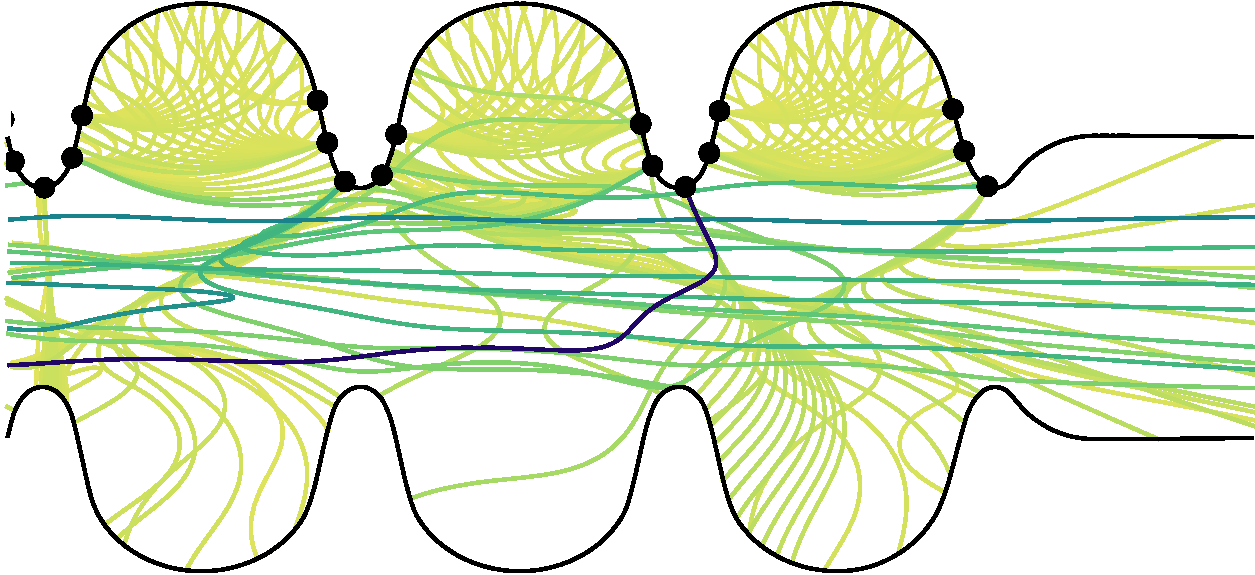
\includegraphics[width=4in]{dark-current.pdf}
  \caption[Dark current tracking.]{
Dark current tracking. Example of where a time based tracker (\vn{time_runge_kutta}) is useful for
simulating particles that can reverse their longitudinal velocity. Here the tracks drawn are from a
simulation of ``dark current'' electrons generated at the walls of an RF cavity due to the large
electromagnetic fields.  }
  \label{f:dark.current}
\end{figure}

\begin{description}

\index{bmad_standard!tracking_method}
\item[\vn{Bmad_Standard}]
Uses formulas for tracking. The formulas generally use the paraxial approximation. The emphasis here
is on speed. It is important to note that field maps (\sref{s:fieldmap}) are {\em ignored} by
\vn{bmad_standard} tracking. The tracking is non-symplectic but the non-symplectic errors tend to
be small so that \vn{bmad_standard} can be used in the vast majority of cases (\sref{s:non.symp}).

\index{custom!tracking_method}
\item[\vn{Custom}]
This method will call a routine \vn{track1_custom} which must be supplied by the programmer
implementing the custom tracking. The default \vn{track1_custom} supplied with the \bmad release
will print an error message and stop the program if it is called which probably indicates a program
linking problem. See \vn{s:custom.ele} for more details.

\index{fixed_step_runge_kutta!tracking_method}
\item[\vn{fixed_step_runge_kutta}]
The \vn{fixed_step_runge_kutta} method is similar to \vn{runge_kutta} tracking except that
\vn{fixed_step_runge_kutta} does not use adaptive step size control but instead takes steps of fixed
size using the setting of \vn{ds_step} or \vn{num_steps} for the element being tracked through
(\sref{s:integ}).  Generally, using adaptive step control will be much more efficient so it is
recommended that \vn{fixed_step_runge_kutta} {\em not} be used unless there is a compelling reason
not to. This method is non-symplectic (\sref{s:non.symp}).

\index{fixed_step_time_runge_kutta!tracking_method}
\item[\vn{fixed_step_time_runge_kutta}]
The \vn{fixed_step_time_runge_kutta} method is similar to \vn{time_runge_kutta} tracking except that
\vn{fixed_step_time_runge_kutta} does not use adaptive step size control but instead takes steps of
fixed size using the setting of \vn{ds_step} or \vn{num_steps} for the element being tracked through
(\sref{s:integ}).  Generally, using adaptive step control will be much more efficient so it is
recommended that \vn{fixed_step_time_runge_kutta} {\em not} be used unless there is a compelling
reason not to. This method is non-symplectic (\sref{s:non.symp}).

\index{linear!tracking_method}
\item[\vn{Linear}]
The \vn{linear} method just tracks particles using the 0th order vector with the 1st order 6x6
transfer matrix of an element. Depending upon how the transfer matrix was generated this may or may
not be symplectic. Since there would be a circular dependency to have the orbital tracking dependent
upon the transfer matrix and the transfer matrix dependent upon the determination of the reference
orbit, the calculation of the transfer matrix when the \vn{tracking_method} is set to \vn{linear}
will always use the zero orbit as the reference orbit.

Additionally, a \vn{linear} tracking method may not be used with \vn{mat6_calc_method} set to
\vn{tracking} since this would also give a circular dependency. Note: setting the
\vn{tracking_method} to \vn{linear} does not affect PTC calculations (\sref{s:ptc.intro}). In
particular, Taylor maps will not be affected.

\index{MAD!tracking_method}
\item[\vn{MAD}]
This uses the MAD 2nd order transfer map. This method is not able to handle element misalignments or
kicks, and becomes inaccurate as the particle energy deviates from the reference energy. MAD
tracking should only be used for testing purposes. Note: Thanks to CERN and Frank Schmidt for
permission to use the MAD tracking code within \bmad.

\index{runge_kutta!tracking_method}
\item[\vn{runge_kutta}]
This uses a 4\Th order Runge Kutta integration algorithm with adaptive step size control.  This is
essentially the Cash-Karp formulation. This method will be slow compared to non-Runge-Kutta methods
so only use this if it is not possible to use something like \vn{bmad_standard}.  This method is
accurate but non-symplectic (\sref{s:non.symp}). \vn{Warning:} When using \vn{custom} fields, if the
fields do not obey Maxwell's equation, there is the possibility of the \vn{runge_kutta} tracking
halting mid-way through an element. See section~\sref{s:integ} for more details.

\index{symp_lie_Bmad!tracking_method}
\item[\vn{Symp_Lie_Bmad}]
Symplectic tracking using a Hamiltonian with Lie operation techniques.  This is similar to
\vn{Symp_Lie_PTC} (see below) except this uses a \bmad routine. By bypassing some of the generality
inherent in PTC (\sref{s:ptc.intro}), \vn{Symp_Lie_Bmad} achieves about a factor of 10 improvement
in speed over \vn{Symp_Lie_PTC}.

\index{symp_lie_ptc!tracking_method}
\item[\vn{Symp_Lie_PTC}]
Symplectic tracking using a Hamiltonian with Lie operator techniques.  This uses \'Etienne Forest's
PTC (\sref{s:ptc.intro}) software for the calculation. This method is symplectic but can be
slow. Exceptions: The tracking is not symplectic when tracking through and element with an
associated electric field and when tracking through a \vn{taylor} element.

\index{taylor!tracking_method}
\item[\vn{Taylor}]
The tracking uses a Taylor map. The map is either explicitly given in the lattice file, that is, the
element must be of type \vn{taylor} (\sref{s:taylor}), or the Taylor map is generated from the PTC
(\sref{s:ptc.intro}) package. Generating the map may take time but once you have it it should be
very fast. One possible problem with using a Taylor map is that you have to worry about the accuracy
if you do tracking at points that are far from the expansion point about which the map was
made. This method is non-symplectic away from the expansion point. Whether the Taylor map is
generated taking into account the offset an element has is governed by the
\vn{taylor_map_includes_offsets} attribute (\sref{s:mapoff}).

The order of a Taylor map is set by the \vn{parameter[taylor_order]}
parameter (\sref{s:param}).

\index{time_runge_kutta!tracking_method}
\item[\vn{Time_Runge_Kutta}]
This method uses time as the independent variable instead of the longitudinal $z$ position. The
advantage of this method is that it can handle particles which reverse direction longitudinally.
One use for this method is ``dark current'' tracking where, as illustrated in \fig{f:dark.current},
low energy particles generated at the vacuum chamber walls can be found traveling in all
directions. Notice that \vn{time_runge_kutta} is different from using \vn{absolute time tracking} as
explained in \sref{s:rf.time}. This method is non-symplectic (\sref{s:non.symp}).

\end{description}

%----------------------------------------------------------------------------

\index{ab_multipole}\index{beambeam}\index{custom}
\index{drift}\index{ecollimator}\index{elseparator}\index{hkicker}
\index{instrument}\index{kicker}\index{lcavity}\index{marker}
\index{match}\index{monitor}\index{multipole}\index{octupole}
\index{patch}\index{quadrupole}\index{rbend}\index{rcollimator}\index{rf_bend}
\index{rfcavity}\index{sbend}\index{sextupole}\index{solenoid}
\index{sol_quad}\index{taylor}\index{vkicker}\index{wiggler}\index{capillary}
\index{element!table of class types}
\begin{table}[pht]
\centering {
\begin{tabular}{lccccccccc}  % \toprule
\rule{0pt}{80pt} 
{\em Element Class} &
\begin{sideways}\vn{Bmad_Standard}\end{sideways} &
\begin{sideways}\vn{Custom}\end{sideways} &
\begin{sideways}\vn{Linear}\end{sideways} &
\begin{sideways}\vn{MAD}\end{sideways} &
\begin{sideways}\vn{Runge_Kutta$^a$}\end{sideways} &
\begin{sideways}\vn{Symp_Lie_Bmad}\end{sideways} &
\begin{sideways}\vn{Symp_Lie_PTC}\end{sideways} &
\begin{sideways}\vn{Taylor}\end{sideways} &
\begin{sideways}\vn{Time_Runge_Kutta$^a$}\end{sideways}
\\ \midrule
%                                     BS   C   L   M   RK    SLB   SLP    T   TRK
  \vn{ab_multipole and multipole}    & D & X & X &   &     &     &  X  &  X  &    \\  
  \vn{ac_kicker}                     & D & X & X &   &  X  &     &     &     & X  \\  
  \vn{beambeam}                      & D & X & X &   &     &     &     &     &    \\  
  \vn{bends: rbend and sbend}        & D & X & X & X &     &     &  X  &  X  &    \\ 
  \vn{converter}                     & D & X &   &   &     &     &     &     &    \\  
  \vn{crab_cavity}                   & D & X & X &   &     &     &     &     &    \\  
  \vn{custom}                        &   & D & X &   &  X  &     &     &     & X  \\  
  \vn{drift}                         & D & X & X & X &  X  &     &  X  &  X  & X  \\  
  \vn{e_gun}                         &   & X &   &   &X$^b$&     &     &     & D  \\  
  \vn{ecollimator and rcollimator}   & D & X & X &   &  X  &     &  X  &  X  & X  \\  
  \vn{elseparator}                   & D & X & X & X &  X  &     &  X  &  X  & X  \\  
  \vn{em_field}                      &   & X &   &   &  D  &     &  X  &  X  & X  \\  
  \vn{fiducial}                      & D & X &   &   &     &     &  X  &     &    \\  
  \vn{floor_shift}                   & D & X &   &   &     &     &  X  &     &    \\  
  \vn{fork}                          & D & X & X &   &     &     &     &     &    \\
  \vn{gkicker}                       & D & X & X &   &     &     &  X  &  X  &    \\
  \vn{hkicker}                       & D & X & X &   &  X  &     &  X  &  X  & X  \\  
  \vn{instrument, monitor, and pipe} & D & X & X &   &  X  &     &  X  &  X  & X  \\  
  \vn{kicker}                        & D & X & X &   &  X  &     &  X  &  X  & X  \\  
  \vn{lcavity and rfcavity}          & D & X & X &   &  X  &     &  X  &  X  & X  \\  
  \vn{marker}                        & D & X & X &   &     &     &  X  &  X  &    \\  
  \vn{match}                         & D & X &   &   &     &     &     &  X  &    \\ 
  \vn{octupole}                      & D & X & X &   &  X  &     &  X  &  X  & X  \\ 
  \vn{patch}                         & D & X &   &   &X$^c$&     &  X  &  X  &    \\ 
  \vn{photonic elements}             & D & X &   &   &     &     &     &     &    \\
  \vn{quadrupole}                    & D & X & X & X &  X  &  X  &  X  &  X  & X  \\ 
  \vn{rf_bend}                       &   & X & X &   &  X  &     &     &     & X  \\
  \vn{sad_mult}                      & D & X & X &   &     &     &  X  &  X  &    \\
  \vn{sextupole}                     & D & X & X & X &  X  &     &  X  &  X  & X  \\ 
  \vn{solenoid}                      & D & X & X & X &  X  &  X  &  X  &  X  & X  \\ 
  \vn{sol_quad}                      & D & X & X &   &  X  &  X  &  X  &  X  & X  \\ 
  \vn{taylor}                        &   & X & X &   &     &     &  X  &  D  &    \\ 
  \vn{vkicker}                       & D & X & X &   &  X  &     &  X  &  X  & X  \\ 
  \vn{wiggler} (map type)            &   & X & X &   &  X  &  X  &  X  &  X  & X  \\
  \vn{wiggler} (periodic type)       & D & X & X &   &X$^d$&X$^d$&X$^d$&D$^d$&    \\ 
  \bottomrule
  \multicolumn{10}{l}{$^a$Includes fixed step versions.}                    \\
  \multicolumn{10}{l}{$^b$Only if the beginning energy is non-zero.}        \\
  \multicolumn{10}{l}{$^c$Only available for non-reflection patch elements.}\\
  \multicolumn{10}{l}{$^d$See \sref{s:wiggler.periodic} for more details.}  \\
\end{tabular}
}
\caption[Table of available tracking_method switches.] { 
Table of valid tracking_method switches. ``D'' denotes the
default method. ``X'' denotes a valid method. Photonic
elements are elements in Table~\ref{t:photon.classes} that cannot be used for
charged particle tracking (Table~\ref{t:particle.classes}).}

\label{t:track.methods}
\end{table}

\vfill \break

%----------------------------------------------------------------------------
\section{Linear Transfer Map (Mat6) Calculation Methods}
\label{s:xfer}
\index{mat6_calc_method|hyperbf}

The \vn{mat6_calc_method} attribute sets how the 6x6 Jacobian transfer matrix for a given element is
computed. Table~\ref{t:mat6.methods} gives which methods are available for each type of element.
Note: Table~\ref{t:mat6.methods} is for charged-particle tracking only. When tracking photons,
transfer matrices (which are not very useful) are not computed.

If an element's \vn{static_linear_map} parameter is set to \vn{True} (the default is \vn{False}),
this prevents the linear map, which consists of the transfer matrix and the zeroth order part of the
map, from being recomputed. For example, if somewhere in a lattice a steering is changed, this will
shift the reference orbit and the linear transfer map in elements where the reference orbit changes
will, in general, vary. However, having \vn{static_linear_map} set to \vn{True} will prevent this
variation.

\index{sympliectify}
\index{taylor_map_includes_offsets}
In addition to the \vn{mat6_calc_method} switch, two element attributes that can affect the way the
transfer matrix is calculated are \vn{symplectify} and \vn{taylor_map_includes_offsets}. These are
discussed in sections \sref{s:symp} and \sref{s:mapoff} respectively.

For methods that do not necessarily produce a symplectic matrix the \vn{symplectify} attribute of an
element can be set to \vn{True} to solve the problem. See \sref{s:symp.method}.

Symplectic integration is like ordinary integration of a function f(x) but what is integrated here
is a Taylor map. Truncating the map to 0\Th order gives the particle trajectory and truncating to
1\St\ order gives the transfer matrix (Jacobian).  The order at which a Taylor series is truncated
at is set by \vn{taylor_order} (see \sref{s:param}. Like ordinary integration there are various
formulas that one can use to do symplectic integration.

\begin{description}

\index{auto!mat6_calc_method}
\item[\vn{Auto}]
With \vn{auto} the \vn{mat6_calc_method} appropriate for the element's setting of
\vn{tracking_method} is used. The correspondence is:
\begin{table}[pth]
\centering {
\begin{tabular}{ll} \toprule
Element's \vn{tracking_method} & \vn{Mat6_calc_method} used\\
\midrule
\vn
  \vn{bmad_standard}         & \vn{bmad_standard} \\
  \vn{linear}                & \vn{bmad_standard} \\
  \vn{custom}                & \vn{custom} \\
  \vn{mad}                   & \vn{mad} \\
  \vn{symp_lie_bmad}         & \vn{symp_lie_bmad} \\
  \vn{symp_lie_ptc}          & \vn{symp_lie_ptc} \\
  \vn{taylor}                & \vn{taylor} \\
  All \vn{Runge-Kutta} types & \vn{tracking} \\
\bottomrule
\end{tabular}
}
\caption[Actual \vn{mat6_calc_method} used with \vn{auto} setting.]{Actual \vn{mat6_calc_method} used when
when the \vn{mat6_calc_method} is set to \vn{auto}.}
\end{table}

\index{bmad_standard!mat6_calc_method}
\item[\vn{Bmad_Standard}]
Uses formulas for the calculation. The formulas generally use the paraxial approximation. The
emphasis here is on speed.

\index{custom!mat6_calc_method}
\item[\vn{Custom}]
This method will call a routine \vn{make_mat6_custom} which must be supplied by the programmer
implementing the custom transfer matrix calculation. The default \vn{make_mat6_custom} supplied with
the \bmad release will print an error message and stop the program if it is called which probably
indicates a program linking problem.  See \vn{s:custom.ele} for more details.

\index{MAD!mat6_calc_method}
\item[\vn{MAD}]
This uses the MAD 2nd transfer map. This method is not able to handle element misalignments or
kicks, and becomes inaccurate as the particle energy deviates from the reference energy. MAD
tracking is generally only used for testing purposes. Thanks must be given to CERN and Frank Schmidt
for permission to use the MAD tracking code within \bmad.

\index{symp_lie_bmad!mat6_calc_method}
\item[\vn{Symp_Lie_Bmad}]
A symplectic calculation using a Hamiltonian with Lie operator techniques.  This is similar to
\vn{Symp_Lie_PTC} (see below) except this uses a \bmad routine. By bypassing some of the generality
inherent in PTC, \vn{Symp_Lie_Bmad} achieves about a factor of 10 improvement in speed over
\vn{Symp_Lie_PTC}. However, \vn{Symp_Lie_Bmad} cannot generate maps above first order.

\index{symp_lie_ptc!mat6_calc_method}
\item[\vn{Symp_Lie_PTC}]
Symplectic integration using a Hamiltonian and Lie operators.  This uses the PTC
(\sref{s:ptc.intro}) software for the calculation.  This method is symplectic but can be
slow. Exceptions: The tracking is not symplectic when tracking through and element with an
associated electric field and when tracking through a \vn{taylor} element.

\index{taylor!mat6_calc_method}
\item[\vn{Taylor}]
This uses a Taylor map generated from \'Etienne's PTC package. Generating the map may take time but
once you have it it should be very fast. One possible problem with using a Taylor map is that you
have to worry about the accuracy if you do a calculation at points that are far from the expansion
point about which the map was made. This method is non-symplectic away from the expansion
point. Whether the Taylor map is generated taking into account the offset an element has is governed
by the \vn{taylor_map_includes_offsets} attribute (\sref{s:mapoff}). \vn{bmad_standard} and
\vn{taylor} tracking methods are identical. Note: Taylor maps for \vn{match}, and \vn{patch}
elements are limited to first order.

The order of a Taylor map is set by the \vn{parameter[taylor_order]}
parameter (\sref{s:param}).

\index{tracking!mat6_calc_method}
\item[\vn{Tracking}]
This uses the tracking method set by \vn{tracking_method} to track 6 particles around the central
orbit. This method is susceptible to inaccuracies caused by nonlinearities. Furthermore this method
is almost surely slow. While non--symplectic, the advantage of this method is that it is directly
related to any tracking results. Note: a \vn{linear} tracking method may not be used with
\vn{mat6_calc_method} set to \vn{tracking} since this would give a circular dependency. The two
parameters that affect this calculation are \vn{bmad_com%d_orb(6)} (\sref{s:bmad.common}) which
sets the six deltas used for displacing the initial particle coordinates from the reference orbit.

\end{description}

\index{ab_multipole}\index{beambeam}\index{custom}
\index{drift}\index{ecollimator}\index{elseparator}\index{hkicker}
\index{instrument}\index{kicker}\index{lcavity}\index{marker}
\index{match}\index{monitor}\index{multipole}\index{octupole}
\index{patch}\index{quadrupole}\index{rbend}\index{rcollimator}
\index{rfcavity}\index{sbend}\index{sextupole}\index{solenoid}
\index{sol_quad}\index{taylor}\index{vkicker}\index{wiggler}
\index{crystal}\index{capillary}\index{rf_bend}
\begin{table}[pth]
\centering {
\begin{tabular}{lcccccccc} \toprule
\rule{0pt}{80pt} &
\begin{sideways}\vn{Bmad_Standard}\end{sideways} &
\begin{sideways}\vn{Custom}\end{sideways} &
\begin{sideways}\vn{MAD}\end{sideways} &
\begin{sideways}\vn{Static}\end{sideways} &
\begin{sideways}\vn{Symp_Lie_Bmad}\end{sideways} &
\begin{sideways}\vn{Symp_Lie_PTC}\end{sideways} &
\begin{sideways}\vn{Taylor}\end{sideways} &
\begin{sideways}\vn{Tracking}\end{sideways}
\\ \midrule
%                                     BS   C   M  Stat SLB   SLP   Tlr  Trk
  \vn{ab_multipole and multipole}    & D & X &   & X &     &  X  &  X  & X \\  
  \vn{ac_kicker}                     &   & X &   & X &     &  X  &  X  & D \\  
  \vn{beambeam}                      & D & X &   & X &     &     &     & X \\  
  \vn{bends: rbend and sbend}        & D & X & X & X &     &  X  &  X  & X \\ 
  \vn{converter}                     & D & X &   &   &     &     &     &   \\  
  \vn{crab_cavity}                   &   & X &   & X &     &     &     & D \\  
  \vn{custom}                        &   & D &   & X &     &     &     & X \\  
  \vn{drift}                         & D & X & X & X &     &  X  &  X  & X \\  
  \vn{e_gun}                         &   & X &   & X &     &     &     & D \\  
  \vn{ecollimator and rcollimator}   & D & X &   & X &     &  X  &  X  & X \\  
  \vn{elseparator}                   & D & X & X & X &     &  X  &  X  & X \\  
  \vn{em_field}                      &   & X &   & X &     &  X  &  X  & D \\  
  \vn{fiducial}                      & D & X &   & X &     &  X  &     & X \\  
  \vn{floor_shift}                   & D & X &   & X &     &  X  &     & X \\  
  \vn{hkicker}                       & D & X &   & X &     &  X  &  X  & X \\  
  \vn{instrument, monitor, and pipe} & D & X &   & X &     &  X  &  X  & X \\  
  \vn{kicker}                        & D & X &   & X &     &  X  &  X  & X \\  
  \vn{lcavity and rfcavity}          & D & X &   & X &     &  X  &  X  & X \\  
  \vn{marker}                        & D & X &   & X &     &  X  &  X  & X \\  
  \vn{match}                         & D & X &   & X &     &     &     & X \\  
  \vn{octupole}                      & D & X &   & X &     &  X  &  X  & X \\ 
  \vn{patch}                         & D & X &   & X &     &  X  &  X  & X \\ 
  \vn{quadrupole}                    & D & X & X & X &  X  &  X  &  X  & X \\ 
  \vn{rf_bend}                       & D & X &   & X &     &     &     & X \\
  \vn{sad_mult}                      & D & X &   & X &     &  X  &  X  & X \\ 
  \vn{sextupole}                     & D & X & X & X &     &  X  &  X  & X \\ 
  \vn{solenoid}                      & D & X & X & X &  X  &  X  &  X  & X \\ 
  \vn{sol_quad}                      & D & X & X & X &  X  &  X  &  X  & X \\ 
  \vn{taylor}                        &   & X &   & X &     &  X  &  D  &   \\ 
  \vn{vkicker}                       & D & X &   & X &     &  X  &  X  & X \\ 
  \vn{wiggler} (map type)            & D & X &   & X &X$^a$&X$^a$&X$^a$& X \\ 
  \vn{wiggler} (periodic type)       &   & X &   & X &X$^a$&X$^a$&D$^a$& X \\ \bottomrule
  \multicolumn{9}{l}{$^a$See \sref{s:wiggler.periodic} for more details} \\
\end{tabular}
} 
\caption[Table of available mat6_calc_method switches.]  {Table of
available mat6_calc_method switches. When tracking photons, transfer
matrices are not computed.  ``D'' denotes the default method. ``X'' denotes an available method.}

\label{t:mat6.methods}
\end{table}

\vfill \break

%----------------------------------------------------------------------------
\section{Spin Tracking Methods}
\label{s:spin.methods}
\index{spin tracking!methods}
\index{spin_tracking_method}

The \vn{spin_tracking_method} attribute of an elements sets the algorithm that is used for tracking
a particle's spin (\sref{s:spin.dyn}) through that element.  Table~\ref{t:spin.methods} gives which
methods are available for each type of element. Note: This table is only for charged-particle tracking
since photons do not have spin.

Possible \vn{spin_tracking_method} settings are:
\begin{description}
%
\index{custom!spin_tracking_method}
\item[\vn{Custom}] \Newline
This method will call a routine \vn{track1_spin_custom} which must be supplied by the programmer
implementing the custom spin tracking calculation. See \vn{s:custom.ele} for more details.
%
\item[\vn{Magnus}] \Newline
This method uses a second-order Magnus expansion of the T-BMT equation to track spins (\sref{s:magnus}).
It is fast and in most cases closely matches numerical integration.
%
\item[\vn{Off}] \Newline
No spin tracking is done and the spin at the end of the element is the same as at the beginning.
%
\item[\vn{Sprint}] \Newline
The \vn{sprint} algorithm (\sref{s:sprint.std}) uses first order transfer spin maps to track the
spin through lattice elements. This method is very fast at the cost of accuracy for particles away
from the zero orbit. The algorithm is also limited in what elements it can handle and it ignores
higher order multipoles that may be present.
%
\index{symp_lie_ptc!spin_tracking_method}
\item[\vn{Symp_Lie_PTC}] \Newline
Symplectic integration using a Hamiltonian and Lie operators.  This uses \'Etienne's PTC software
for the calculation.  This method is symplectic but can be slow.
%
\index{tracking!spin_tracking_method}
\item[\vn{Tracking}] \Newline
How spin is tracked here will depend also on the setting of \vn{tracking_method}. If
\vn{tracking_method} is set to \vn{runge_kutta} or \vn{time_runge_kutta} the spin will be tracked
along with the phase space particle coordinates using the local fields. For \vn{tracking_method} set
to \vn{symp_lie_ptc}, the spin tracking will use \vn{PTC}.  For all other \vn{tracking_method}s, the
spin will be tracked using the ``\vn{bmad_standard}'' spin tracking method which involves Romberg
integration of the spin rotation matrix.

The \vn{runge_kutta} and \vn{time_runge_kutta} spin tracking uses the same fourth order integrator
as is used for the orbital coordinates to track the spin rotation vector.
%
\item[\vn{Transverse_Kick}] \Newline
With a setting of \vn{transverse_kick}, it is assumed that the orbital transfer matrix is due solely
to transverse magnetic fields so that the integrated spin rotation (\Eqs{orpt}, \eq{pqlbp1}, and
\eq{pqlbp2}) can be related to the orbital transport via
\begin{equation}
  \int {\pmb\Omega}_{BMT} = \frac{1 + a \gamma}{1 + p_z} \, (-\Delta p_y, \Delta p_x, 0)
\end{equation}
where $\Delta p_x$ and $\Delta p_y$ are the change in $p_x$ and $p_y$.
Here the small angle approximation ($p_x, p_y \ll 1$) has been used.
\end{description}


%-----------------
Since speed may be an issue, \bmad has an global parameter called \vn{spin_tracking_on} which is
part of the \vn{bmad_com} instance (\sref{s:bmad.ptc.com}) that determines whether spin is tracked or
not. Note: There is also another \vn{bmad_com} parameter called \vn{spin_baier_katkov_flipping_on}
which can influence spin tracking.

\index{spin_fringe_on}
The \vn{spin_fringe_on} element attribute (\sref{s:fringe.at}) can be used to toggle whether the
fringe fields of an element affect the spin.

Example:
\begin{example}
  q: quadrupole, spin_tracking_method = symp_lie_ptc
\end{example}


\index{ab_multipole}\index{beambeam}\index{custom}
\index{drift}\index{ecollimator}\index{elseparator}\index{hkicker}
\index{instrument}\index{kicker}\index{lcavity}\index{marker}
\index{match}\index{monitor}\index{multipole}\index{octupole}
\index{patch}\index{quadrupole}\index{rbend}\index{rcollimator}
\index{rfcavity}\index{sbend}\index{sextupole}\index{solenoid}
\index{sol_quad}\index{taylor}\index{vkicker}\index{wiggler}
\index{crystal}\index{capillary}
\begin{table}[pth]
\centering {
\begin{tabular}{lccccccc} \toprule
\rule{0pt}{80pt} &
\begin{sideways}\vn{Off}\end{sideways} &
\begin{sideways}\vn{Custom}\end{sideways} &
\begin{sideways}\vn{Magnus}\end{sideways} &
\begin{sideways}\vn{Sprint}\end{sideways} &
\begin{sideways}\vn{Symp_Lie_PTC}\end{sideways} &
\begin{sideways}\vn{Tracking}\end{sideways} &
\begin{sideways}\vn{Transverse_Kick}\end{sideways}
\\ \midrule
%                                      O   C   M  Spt SLP Trk TK
  \vn{ab_multipole and multipole}    & X & X &   &   &   & D &   \\  
  \vn{ac_kicker}                     & X & X &   &   &   & D &   \\  
  \vn{beambeam}                      & X & X &   &   &   & D &   \\  
  \vn{bends: rbend and sbend}        & X & X & X & X & X & D &   \\ 
  \vn{converter}                     & X & X &   &   &   & D &   \\  
  \vn{crab_cavity}                   & X & X &   &   &   & D &   \\  
  \vn{custom}                        & X & D &   &   &   & X &   \\  
  \vn{drift}                         & X & X & X & X & X & D &   \\  
  \vn{e_gun}                         & X & X &   &   &   & D &   \\  
  \vn{ecollimator and rcollimator}   & X & X &   & X & X & D &   \\  
  \vn{elseparator}                   & X & X &   &   & X & D &   \\  
  \vn{em_field}                      & X & X &   &   &   & D &   \\  
  \vn{fiducial}                      & X & X &   &   & X & D &   \\  
  \vn{floor_shift}                   & X & X &   &   & X & D &   \\  
  \vn{hkicker}                       & X & X & X & X & X & D &   \\  
  \vn{instrument, monitor and pipe}  & X & X & X & X & X & D &   \\  
  \vn{kicker}                        & X & X & X & X & X & D &   \\  
  \vn{lcavity and rfcavity}          & X & X &   &   & X & D &   \\  
  \vn{marker}                        & X & X &   &   &   & D &   \\  
  \vn{match}                         & D &   &   &   &   &   & X \\  
  \vn{octupole}                      & X & X &   & X & X & D &   \\ 
  \vn{patch}                         & X & X &   &   & X & D &   \\ 
  \vn{quadrupole}                    & X & X & X & X & X & D &   \\ 
  \vn{sad_mult}                      & X & X &   &   &   & D &   \\  
  \vn{sextupole}                     & X & X & X & X & X & D &   \\ 
  \vn{solenoid}                      & X & X & X & X & X & D &   \\ 
  \vn{sol_quad}                      & X & X &   &   & X & D & X \\ 
  \vn{taylor}                        & X &   &   &   &   & D &   \\ 
  \vn{vkicker}                       & X & X & X & X & X & D &   \\ 
  \vn{wiggler}                       & X & X &   &   & X & D &   \\ 
  \bottomrule
\end{tabular}
}

\caption[Table of available spin_tracking_method switches.]{Table of
available \vn{spin_tracking_method}\ switches. ``D'' denotes the default method. 
``X'' denotes an available method. Note: Photon tracking does not involve spin.}

\label{t:spin.methods}
\end{table}

\vfill \break

%-----------------------------------------------------------------
\section{Integration Methods}
\label{s:integ}
\index{integration methods}

\index{symp_lie_bmad!and Taylor maps}
\index{symp_lie_ptc!and Taylor maps}
\index{taylor!and Taylor maps}
``Integration methods'' are tracking methods that involve integrating through an element's magnetic
and electric fields.  Integration methods are split into two classes: Those that can track Taylor
maps and those that simply track a particle's position.  The Taylor map methods are
\begin{example}
  symp_lie_bmad   ! Only to first order
  symp_lie_ptc    ! Uses PTC
  taylor          ! Uses PTC
\end{example}
See section \sref{s:taylor.phys} for more information on Taylor maps and symplectic integration. The
latter two methods involve using the PTC library (\sref{s:ptc.intro}).

The methods that do not involve Taylor maps are
\index{runge_kutta!and Taylor maps}
\begin{example}
  fixed_step_runge_kutta
  fixed_step_time_runge_kutta
  runge_kutta
  time_runge_kutta
\end{example}

\index{ds_step}\index{num_steps}\index{integrator_order}
\index{field_calc}\index{csr_method}\index{space_charge_method}
there are a number of element attributes that can affect the calculation. They are
\begin{example}
  ds_step             = <Real>     ! Integration step length (\sref{s:ds.step})
  num_steps           = <Integer>  ! Number of integration steps. (\sref{s:ds.step})
  integrator_order    = <Integer>  ! Integrator order (\sref{s:ptc.integ})
  field_calc          = <Switch>   ! How the field is calculated (\sref{s:field.calc})
\end{example}

Example:
\begin{example}
  q1: quadrupole, l = 0.6, tracking_method = bmad_standard, 
        mat6_calc_method = symp_lie_ptc, ds_step = 0.2, field_calc = custom
\end{example}

%-----------------------------------------------------------------
\section{CSR and Space Charge Methods}
\label{s:csr.sc.meth}
\index{csr and space charge methods}

When doing beam tracking through an element (\sref{c:multi.sim}), Coherent Synchrotron Radiation
(CSR) and Space Charge (SC) effects can be included by setting the appropriate method switches in
that element. These switches are:
\begin{example}
  csr_method          = <Switch>   ! Coherent Synchrotron Radiation 
  space_charge_method = <Switch>   ! Space charge method
\end{example}
Note: For CSR or SC effects to be included in tracking the \vn{bmad_com} logical
\vn{csr_and_space_charge_on} must be set to \vn{True} (\sref{s:bmad.common}).

The possible settings for \vn{csr_method} are
\begin{example}
  off             ! No CSR. Default.
  1_dim           ! One dimensional calculation (\sref{s:csr.1d}).
\end{example}
The \vn{1_dim} setting cannot be used when \vn{space_charge_method} is set to  \vn{cathode_fft_3d}.

The possible settings of \vn{space_charge_method} are
\begin{example}
  off             ! No SC. Default.
  slice           ! SC using slices (\sref{s:sc.slice}).
  fft_3d          ! SC using a 3D grid (\sref{s:sc.fft}).
  cathode_fft_3d  ! Same as fft_3d with cathode image charge included (\sref{s:sc.fft}).
\end{example}
The \vn{cathode_fft_3d} setting can only be used with \vn{csr_method} set to \vn{off}. Additionally,
the \vn{cathode_fft_3d} setting can only be used with the element \vn{tracking_method} set to
\vn{time_runge_kutta} or \vn{fixed_step_time_runge_kutta}.

Example:
\begin{example}
  q1: quadrupole, l = 0.6, csr_method = 1_dim, space_charge_method = slice, ...
\end{example}

Also see the \vn{space_charge_com} structure (\sref{s:sc.com}) which contains parameters used in
space charge and CSR calculations.

Note: There is also high energy space charge calculation that can be used with single particle
tracking and is discussed in \sref{s:he.space.charge}.

%-----------------------------------------------------------------
\subsection{ds_step and num_steps Parameters}
\label{s:ds.step}
\index{ds_step}\index{num_steps}

\index{taylor}\index{symp_lie_ptc}\index{symp_lie_bmad}
\index{runge_kutta}
One way to create a transfer map through an element is to divide the element up into slices and then
to propagate the transfer map slice by slice.  There are several ways to do this integration. The
\vn{runge_kutta} type methods integrate the equations of motion to give the 0\Th order Taylor map
which just represents a particle's orbit.  Symplectic integration\index{symplectic!integration}
using Lie algebraic techniques, on the other hand, can generate Taylor maps to any order. The
\vn{ds_step} attribute determines the slice thickness.  Alternatively, \vn{num_steps} attribute can
be used in place of \vn{ds_step} to specify the number of slices.  This is applicable to
\vn{symp_lie_bmad} and \vn{symp_lie_ptc} integration. Example:
\begin{example}
  q: quadrupole, l = 0.6, ds_step = 0.1  ! 10 cm step size.
  sbend::*[ds_step] = 0.2                ! Set the step_size for all sbend elements.
\end{example}

When tracking using maps or element-by-element with PTC there are a few points to keep in
mind. First is that \vn{PTC} tracks through a lattice element step by step. This is true for both
map creation and symplectic integration. This means that the setting of the element parameter
\vn{integrator_order} (\sref{s:ptc.integ})
or \vn{num_steps} (or \vn{ds_step}) for each element will affect the accuracy and speed of the
computations. Bmad tries to choose reasonable default settings for the integrator order and number
of steps however the calculation is not perfect. To make sure that the integrator order and number
of steps is set properly, vary both and choose values (which can be different for different
elements) such that the number of steps and integrator order is minimal (to minimize computation
time) while at the same time is large enough so that results do not change significantly if the
number of steps or is varied. Generally it is much better to use a large integrator order and a
small step size rather than vice versa with the proviso that for elements with a longitudinally
varying field (think wigglers or undulators), the step size must be small compared to the typical
longitudinal length scale over which the field is varying (this length scale is the pole period
length with with wigglers and undulators).

The default value for \vn{ds_step} for a given element is calculated based upon the element's field
strength. One should consider the default as more of a guesstimate.

\index{ds_step}
\index{runge_kutta}\index{time_runge_kutta}
\index{rel_tol_adaptive_tracking}\index{abs_tol_adaptive_tracking}
The \vn{runge_kutta} and \vn{time_runge_kutta} tracking uses adaptive step control independent of
the setting of the elements \vn{ds_step} parameter. These methods use three \vn{bmad_com} parameters
\sref{s:bmad.ptc.com}) namely:
\begin{example}
  bmad_com[rel_tol_adaptive_tracking]
  bmad_com[abs_to_adaptive_tracking]
  bmad_com[max_num_runge_kutta_step]
\end{example}
The estimated error of the integration is then bounded by
\begin{example}
  error < abs_tol + |orbit| * rel_tol
\end{example}
lowering the error bounds makes for greater accuracy (as long as round-off 
doesn't hurt) but for slower tracking. 

%-----------------------------------------------------------------
\subsection{Field_calc Parameter}
\label{s:field.calc}
\index{field_calc}

\index{runge_kutta}
The \vn{runge_kutta} type tracking methods all use as input the electric and magnetic fields of
an element. How the EM fields are calculated is determined by the \vn{field_calc} attribute for an
element.  For all lattice elements, except \vn{wigglers} and \vn{undulators}, possible values for
\vn{field_calc} are:
\begin{example}
  bmad_standard     ! This is the default except for custom elements
  custom            ! Default for custom elements.
  fieldmap
\end{example}
For \vn{wigglers} and \vn{undulators}, possible values for \vn{field_calc} are:
\begin{example}
  planar_model
  helical_model
  custom
  fieldmap
\end{example}
\index{custom}\index{runge_kutta}
For historical reasons, the default setting for \vn{field_calc} for \vn{wigglers} and
\vn{undulators} is \vn{planar_model} except if there is a field map present (\sref{s:fieldmap}) in
which case the default is \vn{fieldmap}.  Note that with \vn{bmad_standard} tracking, the setting of
\vn{field_calc} is ignored except in the case of \vn{wigglers} and \vn{undulators} where
\vn{field_calc} must be set to either \vn{planar_model} or \vn{helical_model}.

\vn{Custom} means that the field calculations are done outside of the \bmad software. A program
doing \vn{custom} field calculations will need the appropriate custom routine (\sref{s:custom.ele}).
Elements that set \vn{field_calc} to \vn{fieldmap} need to have a field map defined
(\sref{s:fieldmap}).

\vn{Warning:} When tracking a particle through a custom field using \vn{runge_kutta}, it is
important that the field obey Maxwell's equations. Fields that do not obey Maxwell's Equations may
cause the \vn{runge_kutta} adaptive step size control algorithm to take smaller and smaller steps
until the step size becomes so small the tracking will stop. What happens is that the step size
control algorithm takes a step and then takes two half steps over the same region and from this
estimates the error in the calculation. If the error is larger than the allowed tolerance the
control algorithm shortens the step and tries again. A field that does not obey Maxwell's equations
can fool the control algorithm into thinking that the error is always larger than the allowed
tolerance for any finite step size. A typical situation is where the field has an unphysical step
across some boundary.

%-----------------------------------------------------------------
\subsection{PTC Integration}
\label{s:ptc.integ}
\index{PTC integration}

\index{integrator_order}
\index{ds_step}\index{symp_lie_bmad}
The \vn{integrator_order} element attribute is the order of the integration formula for
\vn{Symp_Lie_PTC} and is used for constructing Taylor maps. Possible values are
\begin{example}
  integrator_order = 2, 4, 6, or 8
\end{example}
Essentially, an integrator order of $n$ means that the error in an integration step scales as
$dz^{n+1}$ where $dz$ is the slice thickness. For a given number of steps a higher order will give
more accurate results but a higher order integrator will take more time per step. It turns out that
for wigglers, after adjusting \vn{ds_step} for a given accuracy, the order 2 integrator is the
fastest. This is not surprising given the highly nonlinear nature of a wiggler. Note that
\vn{symp_lie_bmad} always uses an order 2 integrator independent of the setting of
\vn{integrator_order}. The setting of \vn{8} is not implemented for all elements. If \vn{8} is set
for a given element type that does not support it, a value of \vn{6} will be used instead.

\index{exact_model}\index{exact_misalign}
When tracking uses the \vn{PTC} library (\sref{s:ptc.intro}), there are two global parameters that
can be set in the lattice file that affect the calculation. These are:
\begin{example}
  ptc_com[exact_model]    = <Logical>  ! "exact" tracking? Default: False
  ptc_com[exact_misalign] = <Logical>  ! "exactly" misalign elements? Default: True
\end{example}
The default for \vn{exact_model} is \vn{True} and the default for \vn{exact_misalign} is \vn{True}.

The \vn{exact_model} parameter sets whether PTC uses an ``exact'' model for
tracking. Essentially this means that the paraxial approximation (\sref{s:mag.hamiltonian}) is made
for \vn{exact_model} set to \vn{False} and is not made if set to \vn{True}. This can be
important, for example, for bend tracking when the bend radius is small.

In PTC, exact modeling can be set on an element-by-element basis. Currently \bmad does not support
specifying element-by-element setting of exact modeling. However, PTC does not have a non-exact
tracking option for elements that have an electric field. In this case, PTC tracking will always be
exact independent of the setting of \vn{exact_model}.  Additionally, for elements with an
electric field, tracking will not be symplectic.

The \vn{exact_misalign} parameter determines whether misalignments are handled exactly or
whether approximations are made that will speed up the calculation.

In addition to the above parameters, how the Hamiltonian is split when tracking with \vn{PTC} can be
set for individual elements using the \vn{ptc_integration_type} parameter. Possible settings of this
parameter are
\begin{example}
  drift_kick    ! See Eq. (125) of \cite{b:geo.int}
  matrix_kick   ! See Eq. (132) of \cite{b:geo.int}. Default
  ripken_kick   ! See Eq. (130) of \cite{b:geo.int}
\end{example}
Example:
\begin{example}
  q2: quad, l = 0.6, k1 = 0.34, ptc_integration_type = drift_kick
\end{example}
A discussion of the different types of integration schemes is given by Forest\cite{b:geo.int}. The
equation that shows the appropriate splitting of the Hamiltonian for each integration type is
referenced in the above list. The \vn{ripken_kick} type is for benchmarking with the \vn{SixTrack}
program and is not otherwise generally useful. The difference between \vn{drift_kick} and
\vn{matrix_kick} is that with \vn{drift_kick} the quadrupolar part of the magnetic multipole is is
included in the applied kick between drifts while in the \vn{matrix_kick} method the quadrupolar
component is used for the ``matrix'' tracking between kicks. With the \vn{matrix_kick} method the
tune of a machine tends to be insensitive to how many integration steps (set by \vn{ds_step} or
\vn{n_steps}) are used.

PTC does not implement \vn{matrix_kick} tracking for elements with an electric field. In this case,
the setting of \vn{ptc_integration_type} is ignored and tracking will be \vn{drift_kick}. Thus, if
an electric field is introduced into an element, more integration steps may be required to get the
correct tune.

%-----------------------------------------------------------------
\section{Symplectic Versus Non-Symplectic Tracking}
\label{s:non.symp}
\index{symplectify}

When selecting tracking methods for lattice elements, there are several factors to consider,
including symplecticity. Despite its emphasis in accelerator textbooks, symplecity (or the lack
therof) is typically only relevant for long-term tracking when there is minimal radiation emission
over many turns. That is, the potential problem with non-symplectic tracking is the buildup of
errors over many turns. Thus, computations that involve only tracking through the lattice from
beginning to end -- like calculating Twiss functions or tracking through a linac -- generally do not
benefit from symplectic tracking. More important in these cases is the speed of the calculation, 
which can be obtained with the cost of non-symplecticity.

The motion of particles that radiate is not symplectic. Thus, symplectic tracking for the
non-radiative part of the motion may not be needed if radiation is large enough. For example, for
simulations of the Cornell CESR ring with electron and positron beam energies of order 1~GeV to
10~GeV and with damping times on the order of 10,000 turns, the \vn{bmad_standard} tracking has
proved quite adequate. However in other cases with radiation, the symplectic error may cause an 
extra damping or anti-damping effect, giving equilibrium beam sizes that are an under/overestimate 
of the actual beam sizes. When opting for speed versus symplecticity in long term tracking over 
many turns, care should be taken to ensure that the effects of the non-symplecticity are minimal.

%-----------------------------------------------------------------
\section{Symplectify Attribute}
\label{s:symp}
\index{symplectify|hyperbf}

The \vn{symplectify} attribute
\begin{example}
  symplectify = <Logical>
\end{example}
is used to make the transfer matrix for an element symplectic. The linear transport matrix may be
non--symplectic for a number of reasons.  For example, the linear matrix that comes from expanding a
Taylor Map around any point that is not the origin of the map is generally not symplectic. The
transfer matrix for an element can be symplectified by setting the \vn{symplectify} attribute to
True. See section~\sref{s:symp.method} for details on how a matrix is symplectified. The default
value of \vn{symplectify}, if it is not present, is \vn{False}. If it is present without a value
then it defaults to true. Examples:
\begin{example}
  s1: sextupole, l = 0.34                       ! symplectify = False
  s1: sextupole, symplectify = True, l = 0.34   ! symplectify = True
  s1: sextupole, symplectify, l = 0.34          ! symplectify = True
\end{example}

\label{lcavity} Note that for elements like an \vn{lcavity} where the
reference momentum at the downstream end of the element is different
from the upstream end, the transfer matrix is never symplectic. In
this case, ``symplectification'' involves first transforming the
transfer matrix so that the reference momentum is the same upstream
and downstream, then performing symplectification, and finally back
transforming the reference momentum to their original values.

%-----------------------------------------------------------------
\section{taylor_map_include_offsets Attribute}
\label{s:mapoff}
\index{taylor_map_includes_offsets|hyperbf}

The \vn{taylor_map_includes_offsets} attribute sets whether the Taylor map
generated for an element includes the affect due to the elements
(mis)orientation in space. That is, the affect of any pitches, offsets
or tilt (\sref{s:offset}). The default is \vn{True} which means that
the Taylor map will include such effects. 

How \vn{taylor_map_includes_offsets} is set will not affect the results of
tracking or the Jacobian matrix calculation. What is affected is the
speed of the calculations. With \vn{taylor_map_includes_offsets} set to \vn{True}
the Taylor map will have to be recalculated each time an element is
reoriented in space. On the other hand, with \vn{taylor_map_includes_offsets} set
to \vn{False} each tracking and Jacobian matrix calculation will
include the extra computation involving the effect of the
orientation. Thus if an element's orientation is fixed it is faster to
set \vn{taylor_map_includes_offsets} to \vn{True} and if the orientation is
varying it is faster to set \vn{taylor_map_includes_offsets} to \vn{False}.

If the global parameter \vn{bmad_com%conserve_taylor_maps}
(\sref{s:bmad.ptc.com}) is set to True (the default), then, if an
element is offset within a program, and if \vn{taylor_map_include_offsets} is set
to True for that element, \bmad will toggle \vn{taylor_map_include_offsets} to
False to conserve the map.

\chapter{Beam Lines and Replacement Lists}
\label{c:sequence}

\index{branch}
This chapter describes how to define the ordered list of elements that make up a lattice branch
(\sref{s:branch.def}).  In a lattice, branches may be connected together using \vn{fork} or
\vn{photon fork} elements (\vn{s:fork}), or by using \vn{multipass} (\sref{c:multipass}).

%-----------------------------------------------------------------------------
\section{Branch Construction Overview}
\label{s:branch.construct}

\index{list}
A lattice branch (\sref{s:branch.def}) is defined in a lattice file using what are called \vn{beam lines}
(\sref{s:lines.wo.arg}) and \vn{replacement lists} (\sref{s:replace.list}).  The \vn{beam lines} are
divided into two types - lines with (\sref{s:lines.with.arg}) and lines without
(\sref{s:lines.wo.arg}) \vn{replacement arguments}. This essentially corresponds to the \mad
definition of lines and lists. There can be multiple \vn{beam lines} and \vn{replacement lists}
defined in a lattice file and lines and lists can be nested inside other lines and lists.

Since lines can be nested within other lines, The same element name may be repeated multiple times
in a branch. To distinguish between multiple elements of the same name, lines and lists may be
\vn{tagged} (\sref{s:tag}) to produce unique element names.

A marker element named \vn{END} will, by default, be placed at the ends of all the branches unless a
\vn{parameter[no_end_marker]} statement (\sref{s:param}) is used to suppress the insertion.
Additionally, if an ending marker named \vn{END} is already present in the lattice file, no extra
marker will be created.

Branches are ordered in an array (\sref{s:lattice.def}) and each branch is assigned an index number
starting with index 0. When there are multiple branches in a lattice, the reference orbit
(\sref{s:ref}) of a branch must not depend upon details of branches later on in the array.  \bmad
depends upon this and calculates the reference orbits of the branches one at a time starting with
the first branch.

%-----------------------------------------------------------------------------
\section{Beam Lines and Lattice Expansion}
\label{s:lines.wo.arg}
\index{line|hyperbf}

A \vn{beam line} without arguments has the format
\begin{example}
  label: line = (member1, member2, ...)
\end{example}
where \vn{member1}, \vn{member2}, etc. are either elements, other \vn{beam lines} or \vn{replacement
lists}, or sublines enclosed in parentheses.  Example:
\begin{example}
  line1: line = (a, b, c)
  line2: line = (d, line1, e)
  use, line2
\end{example}
The \vn{use} statement is explained in Section~\sref{s:use}.  This example shows how a \vn{beam
line} member can refer to another \vn{beam line}. This is helpful if the same sequence of elements
appears repeatedly in the lattice.

The process of constructing the ordered sequences of elements that comprise the branches of the
lattice is called \vn{lattice expansion}. In the example above, when \vn{line2} is expanded to form
the lattice (in this case there is only one branch so \vn{lattice} and \vn{branch} can be considered
synonymous), the definition of \vn{line1} will be inserted in to produce the following lattice:
\begin{example}
  beginning, d, a, b, c, e, end
\end{example}
The \vn{beginning} and \vn{end} marker elements are automatically inserted at the beginning and end
of the lattice. The \vn{beginning} element will always exist but insertion of the \vn{end} element
can be suppressed by inserting into the lattice:
\begin{example}
 parameter[no_end_marker] = T    ! See: \sref{s:param}
\end{example}
Lattice expansion occurs either at the end after the lattice file has been parsed, or, during parsing, at the
point where an \vn{expand_lattice} statement (\sref{s:expand}) is found.

Each element is assigned an \vn{element index} number starting from 0 for the \vn{beginning}
element, 1 for the next element, etc.

In the expanded lattice, any \vn{null_Ele} type elements (\sref{s:null.ele}) will be discarded. For
example, if element \vn{b} in the above example is a \vn{null_Ele} then the actual expanded lattice
will be:
\begin{example}
  beginning, d, a, c, e, end
\end{example}

\index{reflection of elements}
A member that is a line or list can be ``reflected'' (elements taken in reverse order) if a negative
sign is put in front of it. For example:
\begin{example}
  line1: line = (a, b, c)
  line2: line = (d, -line1, e)
\end{example}
\vn{line2} when expanded gives
\begin{example}
  d, c, b, a, e
\end{example}
It is important to keep in mind that line reflection is \vn{not} the same as going backwards through
elements. For example, if an \vn{sbend} or \vn{rbend} element (\sref{s:bend}) is reflected, the
face angle of the upstream edge (\sref{s:ref.construct}) is still specified by the \vn{e1} attribute
and not the \vn{e2} attribute. True element reversal can be accomplished as discussed in \Sref{s:ele.reverse}.

Reflecting a subline will also reflect any sublines of the subline. For example:
\begin{example}
  line0: line = (y, z)
  line1: line = (line0, b, c)
  line2: line = (d, -line1, e)
\end{example}
\vn{line2} when expanded gives
\begin{example}
  d, c, b, z, y, e
\end{example}
\index{sbend}\index{rbend}

A repetition count, which is an integer followed by an asterisk, 
means that the member is
repeated. For example
\begin{example}
  line1: line = (a, b, c)
  line2: line = (d, 2*line1, e)
\end{example}
\vn{line2} when expanded gives
\begin{example}
  d, a, b, c, a, b, c, e
\end{example}
Repetition count can be combined with reflection. For example
\begin{example}
  line1: line = (a, b, c)
  line2: line = (d, -2*line1, e)
\end{example}
\vn{line2} when expanded gives
\begin{example}
  d, c, b, a, c, b, a, e
\end{example}
Instead of the name of a line, subline members can also be given as an explicit list using
parentheses. For example, the previous example could be rewritten as
\begin{example}
  line2: line = (d, -2*(a, b, c), e)
\end{example}

Lines can be defined in any order in the lattice file so a subline does not have to come before a
line that references it. Additionally, element definitions can come before or after any lines that
reference them.

A line can have the \vn{multipass} attribute. This is covered in \sref{c:multipass}.

%-----------------------------------------------------------------------------
\section{Line Slices}
\label{s:line.slice}
\index{line slice}

A line ``\vn{slice}'' is a section of a line from some starting element to some ending element.  A
line slice can be used to construct a new line similar to how an unsliced line is used to construct
a new line. An example will make this clear:
\begin{example}
  line1: line = (a, b, c, d, e)
  line2: line = (z1, line1[b:d], z2)
\end{example}
The line slice \vn{line1[b:d]} that is used to construct \vn{line2} consists of the elements in
\vn{line1} from element \vn{b} to element \vn{d} but not elements \vn{a} or \vn{e}. When \vn{line2}
is expanded, it will have the elements:
\begin{example}
  z1, b, c, d, z2
\end{example}

The general form for line slices is
\begin{example}
  line_name[element1:element2]
\end{example}
where \vn{line_name} is the name of the line and \vn{element1} and \vn{element2} delimit the
beginning and ending positions of the slice. The beginning and ending element names may be omitted
and, if not present, the default is the beginning element and ending element of the line
respectively. Thus, for example, ``\vn{line4[:q1]}'' represents the list of elements from the start
of \vn{line4} up to, and including the element \vn{q1}.

If there are multiple elements of the same name, the double hash \vn{\#\#} symbol
(\sref{s:ele.match}) can be use to denote the N\Th element of a given name. If double hash is not
used, the first instance of a given element name is assumed. That is, something like ``\vn{q1}'' is
equivalent to ``\vn{q1\#\#1}''.

Wild card characters and \vn{class::element_name} syntax (\sref{s:ele.match}) are not allowed with
slice element names.

Line slicing of a given line occurs after the line has been expanded (all sublines and line slices
substituted in). Thus, the following makes sense:
\begin{example}
  line1: line = (a, b, c, d, e)
  line2: line = (z1, line1, z2)
  line3: line = (line2[z1:c])
\end{example}

%-----------------------------------------------------------------------------
\section{Element Orientation Reversal}
\label{s:ele.reverse}
\index{element reversal}

An element's orientation is \vn{reversed} if particles traveling through it enter at the ``exit'' end and leave at
the ``entrance'' end. Being able to reverse elements is useful, for example, in describing the
interaction region of a pair of rings where particles of one ring are going in the opposite
direction relative to the particles in the other ring.

Element reversal is indicated by using a double negative sign ``$--$'' prefix. The double negative
sign prefix can be applied to individual elements or to a line. If it is applied to a line, the line
is both reflected (same as if a single negative sign is used) and each element is reversed. For
example:
\begin{example}
  line1: line = (a, b, --c)
  line2: line = (--line1)
  line3: line = (c, --b, --a)
\end{example}
In this example, \vn{line2} and \vn{line3} are identical. Notice that the reversal of a reversed
element makes the element unreversed.

Another example involving element reversal is given in Section~\sref{s:reverse}.

Reversed elements, unlike other elements, have their local $z$-axis pointing in the opposite
direction to the local $s$-axis (\sref{s:ref.construct}). This means that there must be a
\vn{reflection patch} (\sref{s:reflect.patch}) between reversed and unreversed elements. Since this
complicates matters, it is generally only useful to employ element reversal in cases where there are
multiple intersecting lines with particle beams going in opposite directions through some elements
(for example, colliding beam interaction regions). In this case, element reversal is typically used
with \vn{multipass} (\sref{c:multipass}) and the lattice will contain a branch of unreversed
elements for simulating particles going in one direction along with a branch of reversed elements to
simulate particle going in the other direction.

Where reversed elements are not needed, it is simple to define elements that are
effectively reversed. For example:
\begin{example}
  b00: bend, angle = 0.023, e1 = ...
  b00_rev: b00, angle = -b00[angle], e1 = -b00[e2], e2 = -b00[e1]
\end{example}
and \vn{b00_rev} serves as a reversed version of \vn{b00}.

Internally, \bmad associates an \vn{orientation} attribute with each element. This attribute is set
to -1 for reversed elements and 1 for unreversed elements.

%-----------------------------------------------------------------------------
\section{Beam Lines with Replaceable Arguments}
\label{s:lines.with.arg}
\index{line!with arguments}

\vn{Beam lines} can have an argument list using the following syntax
\begin{example}
  line_name(dummy_arg1, dummy_arg2, ...): LINE = (member1, member2, ...)
\end{example}
The dummy arguments are replaced by the actual arguments when the line is used
elsewhere. For example:
\begin{example}
  line1(DA1, DA2): line = (a, DA2, b, DA1)
  line2: line = (h, line1(y, z), g)
\end{example}
When \vn{line2} is expanded the actual arguments of \vn{line1}, in this case \vn(y, z), replaces the
dummy arguments \vn{(DA1, DA2)} to give for \vn{line2}
\begin{example}
  h, a, z, b, y, g
\end{example} 
\index{MAD}
Unlike \mad, \vn{beam line} actual arguments can only be elements or \vn{beam lines}. 
Thus the following is not allowed
\begin{example}
  line2: line = (h, line1(2*y, z), g)   ! NO: 2*y NOT allowed as an argument.
\end{example}

%-----------------------------------------------------------------------------
\section{Lists}
\label{s:replace.list}
\index{list|hyperbf}

When a lattice is expanded, all the lattice members that correspond to a name of a \vn{list} are
replaced successively, by the members in the \vn{list}. The general syntax is
\begin{example}
  label: LIST = (member1, member2, ...)
\end{example}
For example:
\begin{example}
  my_list1 list = (a, b, c)
  line1: line = (z1, my_list, z2, my_list, z3, my_list, z4, my_list)
  use, line1
\end{example}
When the lattice is expanded the first instance of \vn{my_list} in \vn{line1} is replaced by \vn{a}
(which is the first element of \vn{my_list}), the second instance of \vn{my_list} is replaced by
\vn{b}, etc. If there are more instances of \vn{my_list} in the lattice then members of
\vn{my_list}, the replacement starts at the beginning of \vn{my_list} after the last member of
\vn{my_list} is used. In this case the lattice would be:
\begin{example}
  z1, a, z2, b, z3, c, z4, a
\end{example}
members of a \vn{replacement list} can only be simple elements and not other lines or lists. 
For example, the following is not allowed:
\begin{example}
  line1: line = (a, b)
  my_list: list = (2*line1)  ! Lines cannot be list members.
\end{example}
A repetition count is permitted
\begin{example}
  my_list1: list = (2*a, b) 
  my_list2: list = (a, a, b) ! Equivalent to my_list1
\end{example}

%-----------------------------------------------------------------------------
\section{Use Statement}
\label{s:use}

\index{use statement|hyperbf}
The particular line or lines that defines the root branches (\sref{s:lattice.def}) to be used in the
lattice is selected by the \vn{use} statement. The general syntax is
\begin{example}
  use, line1, line2 ...
\end{example}
For example, \vn{line1} may correspond to one ring and \vn{line2} may correspond to the other ring
of a dual ring colliding beam machine. In this case, \vn{multipass} (\sref{c:multipass}) will be
needed to describe the common elements of the two rings. Example
\begin{example}
  use, e_ring, p_ring
\end{example}
would pick the lines \vn{e_ring} and \vn{p_ring} for analysis.  These will be the \vn{root}
branches.

\vn{use} statements can come anywhere in the lattice, even before the definition of the lines they
refer to. Additionally, there can be multiple \vn{use} statements.  The last \vn{use} statement in
the file defines which \vn{line} to use.

The total number of branches in the lattice is equal to the number of lines that appear on the
\vn{use} statement plus the number of \vn{fork} and \vn{photon_fork} elements that branch to a new
branch.

To set such things as the geometry of a branch, beginning Twiss parameters, etc., see Section
\vn{s:beginning}.

%-----------------------------------------------------------------------------
\section{Tagging Lines and Lists}
\index{tags for lines and lists|hyperbf}
\label{s:tag}

When a lattice has repeating lines, it can be desirable to differentiate
between repeated elements. This can be done by tagging lines with a \vn{tag}. 
An example will make this clear:
\begin{example}
  line1: line = (a, b)
  line2: line = (line1, line1)
  use, line2
\end{example}
When expanded the lattice would be:
\begin{example}
  a, b, a, b
\end{example}
The first and third elements have the same name ``a'' and the second and fourth
elements have the same name ``b''. Using tags the lattice elements can be given
unique names. lines or lists are tagged  
using the at (@) sign. The general syntax is:
\begin{example}
  tag_name@line_name                           ! Syntax for lines
  tag_name@list_name                           ! Syntax for lists
  tag_name@replacement_line(arg1, arg2, ...)   ! Syntax for replacement lines.
\end{example}
Thus to differentiate the lattice elements in the above example \vn{line2} needs to
be modified using tags:
\begin{example}
  line1: line = (a, b)
  line2: line = (t1@line1, t2@line1)
  use, line2
\end{example}
In this case the lattice elements will have names of the form:
\begin{example}
  tag_name.element_name
\end{example}
In this particular example, the lattice with tagging will be:
\begin{example}
  t1.a, t1.b, t2.a, t2.b
\end{example}
Of course with this simple example one could have just as easily not used tags:
\begin{example}
  t1.a: a;   t2.a: a
  t1.b: b;   t2.b: b
  line1: line = (t1.a, t1.b, t2.a, t2.b)
  use, line2
\end{example}
But in more complicated situations tagging can make for compact lattice files.

When lines are nested, the name of an element is formed by concatenating the tags together with dots
in between in the form:
\begin{example}
  tag_name1.tag_name2. ... tag_name_n.element_name
\end{example}
An example will make this clear:
\begin{example}
  list1 = (g, h)
  line1(y, z) = (a, b)
  line2: line = (t1@line1(a, b))
  line3: line = (line2, hh@list1)
  line4: line = (z1@line3, z2@line3)
  use, line4
\end{example}
The lattice elements in this case are:
\begin{example}
  z1.t1.a, z1.t1.b, z1.hh.g, z2.t1.a, z2.t1.b, z1.hh.h 
\end{example}

\index{expand_lattice}
To modify a particular tagged element the lattice must be expanded
first (\sref{s:expand}). For example:
\begin{example}
  line1: line = (a, b)
  line2: line = (t1@line1, t2@line1)
  use, line2
  expand_lattice
  t1.b[k1] = 1.37
  b[k1] = 0.63       ! This statement generates an error
\end{example}
After the lattice has been expanded there is no connection between the original \vn{a} and \vn{b}
elements and the elements in the lattice like \vn{t1.b}. Thus the last line in the example where the
\vn{k1} attribute of\vn{b} is modified generates an error since there are no elements named \vn{b}
in the lattice.

\chapter{Superposition}
\label{c:super}

\index{superposition}
This chapter covers the concept of \vn{superposition}.  \vn{Superposition} is used when elements
overlap spatially.  With \vn{superposition}, \vn{lord} and \vn{slave} elements (\sref{s:lord.slave})
are constructed by \bmad to hold the necessary information. The \vn{lord} elements will represent
the ``physical'' element while the \vn{slave} elements will embody the ``beam path''.

%-----------------------------------------------------------------------------
\section{Superposition Fundamentals}
\label{c:super.fund}

  \begin{figure}[tb]
  \centering 
  \includegraphics[width=0.95\textwidth]{superimpose-example.pdf} 
  \caption[Superposition example.]
{Superposition example. A) The physical layout involves a quadrupole partially inside a solenoid. B)
The standard superposition procedure involves creating \vn{super_slave} elements whose edges are at
the boundaries where the physical elements overlap. C) When jumbo \vn{super_slaves} are created, the
\vn{super_slaves} span the entire space where elements overlap.}
  \label{f:super.ex}
  \end{figure}

In practice the field at a particular point in the lattice may be due to more than one physical
element. One example of this is a quadrupole magnet inside a larger solenoid magnet as shown in
\fig{f:super.ex}A. \bmad has a mechanism to handle this using what is called ``superposition''. A
simple example shows how this works (also see section \sref{s:lord.slave}):
\begin{example}
  Q: quad, l = 4
  D: drift, l = 12
  S: solenoid, l = 8, superimpose, ref = Q, ele_origin = beginning
  M: marker, superimpose, ref = S, offset = 1
  lat: line = (Q, D)
  use, lat
\end{example}
The \vn{superimpose} attribute of element \vn{S} superimposes \vn{S} over the lattice \vn{(Q,
D)}. The placement of \vn{S} is such that the beginning of \vn{S} is coincident with the center of
\vn{Q} (this is is explained in more detail below). Additionally, a marker \vn{M} is superimposed at
a distance of +1~meter from the center of \vn{S}. The tracking part of the lattice
(\sref{s:lord.slave}) looks like:
\begin{example}
        Element   Key         Length  Total     
  1)    Q{\#}1       Quadrupole   2        2
  2)    Q{\B}S       Sol_quad     2        4
  3)    S{\#}1       Solenoid     3        7
  4)    M         Marker       0      
  4)    S{\#}2       Solenoid     3       10
  5)    D{\#}2       Drift        4       14
\end{example}
What \bmad has done is to split the original elements \vn{(Q, D)} at the edges of \vn{S} and then
\vn{S} was split where \vn{M} is inserted. The first element in the lattice, \vn{Q\#1}, is the part
of \vn{Q} that is outside of \vn{S}. Since this is only part of \vn{Q}, \bmad has put a \vn{\#1} in
the name so that there will be no confusion. (a single \vn{\#} has no special meaning other than the
fact that \bmad uses it for mangling names. This is opposed to a double \vn{\#\#} which is used to
denote the $N$\Th instance of an element (\sref{s:ele.match}). The next element, \vn{Q{\B}S}, is the
part of \vn{Q} that is inside \vn{S}. \vn{Q{\B}S} is a combination solenoid/quadrupole element as
one would expect. \vn{S{\#}1} is the part of \vn{S} that is outside \vn{Q} but before \vn{M}. This
element is just a solenoid. Next comes \vn{M}, \vn{S{\#}1}, and finally \vn{D\#2} is the rest of the
drift outside \vn{S}.

In the above example, \vn{Q} and \vn{S} will be \vn{super_lord} elements (\vn{s:lord.slave}) and
four elements in the tracking part of the lattice will be \vn{super_slave} elements. This is
illustrated in \fig{f:super.ex}B.

Notice that the name chosen for the \vn{sol_quad} element \vn{Q{\B}S} is dependent upon what is
being superimposed upon what. If \vn{Q} had been superimposed upon \vn{S} then the name would have
been \vn{S{\B}Q}.

When \bmad sets the element class for elements created from superpositions, \bmad will set the class
of the element to something other than an \vn{em_field} element (\sref{s:em.field}) if possible. If
no other possibilities exist, \bmad will use \vn{em_field}. For example, a \vn{quadrupole}
superimposed with a \vn{solenoid} will produce a \vn{sol_quad} \vn{super_slave} element but a
\vn{solenoid} superimposed with a \vn{rfcavity} element will produce an \vn{em_field} element since
there is no other class of element that can simultaneously handle solenoid and RF fields. An
\vn{em_field} \vn{super_slave} element will also be created if any of the superimposing elements 
have a non-zero orientation (\sref{s:offset}) since it is not, in general, possible to construct a slave
element that properly mimics the effect of a non-zero orientation.

  \begin{figure}[tb]
  \centering 
  \includegraphics[width=0.8\textwidth]{superimpose.pdf} 
  \caption[Superposition Offset.]{
The superposition offset is the distance along the local reference orbit from the origin point of the
reference element to the origin point of the element being superimposed.
  }
  \label{f:superimpose}
  \end{figure}

With the lattice broken up like this \bmad has constructed something that can be easily
analyzed. However, the original elements \vn{Q} and \vn{S} still exist within the lord section of
the lattice. \bmad has bookkeeping routines so that if a change is made to the \vn{Q} or \vn{S}
elements then these changes can get propagated to the corresponding slaves. It does not matter which
element is superimposed. Thus, in the above example, \vn{S} could have been put in the Beam Line
(with a drift before it) and \vn{Q} could then have been superimposed on top and the result would
have been the same (except that the split elements could have different names).

If an element has zero length (for example, a \vn{marker} element), is superimposed, or is
superimposed upon, then the element will remain in the tracking part of the lattice and there will
be no corresponding lord element. See \fig{f:super.ex}.
 
Superimpose syntax:
\begin{example}
  Q: quad, superimpose, ...       ! Superimpose element Q.
  Q: quad, superimpose = T, ...   ! Same as above.
  Q: quad, ...                    ! First define element Q ...
  Q[superimpose] = T              !   ... and then superimpose.
  Q[superimpose] = F              ! Suppress superposition.
\end{example}
Superposition happens at the end of parsing so the last set of the \vn{superimpose} for an element
will override previous settings. 

It is also possible to superimpose an element using the \vn{superimpose} command which has the
syntax:
\begin{example}
  superimpose, element = <ele-name>, ...
\end{example}
With the same optional superposition parameters (\vn{ref}, \vn{offset}, etc.) given below.
Example:
\begin{example}
  superimpose, element = Q1, ref = B12, offset = 1.3, 
                               ele_origin = beginning, ref_origin = end
\end{example}
Note: Superposition using the superimpose statement allows superimposing the same element with
multiple reference elements and/or multiple offsets. The drawback is that superposition using the
superimpose statement may not be switched off later in the lattice file.

The placement of a superimposed element is illustrated in \fig{f:superimpose}. The placement of a
superimposed element is determined by three factors: An origin point on the superimposed element, an
origin point on the reference element, and an offset between the points. The attributes that
determine these three quantities are:
\index{ref}\index{offset}
\index{ref_origin}\index{ele_origin}
\begin{example}
  create_jumbo_slave = <Logical>     ! See \sref{s:jumbo.slave}
  wrap_superimpose   = <Logical>     ! Wrap if element extends past lattice ends?
  ref          = <lattice_element>
  offset       = <length>            ! default = 0
  ele_origin   = <origin_location>   ! Origin pt on element.
  ref_origin   = <origin_location>   ! Origin pt on ref element.
\end{example}
\vn{ref} sets the reference element. If \vn{ref} is not present then the start of the lattice is
used (more precisely, the start of branch 0 (\sref{s:branch.def})). Wild card characters
(\sref{s:ele.match} can be used with \vn{ref}. If \vn{ref} matches to multiple elements (which may
also happen without wild card characters if there are multiple elements with the name given by
\vn{ref}) in the lattice a superposition will be done, one for each match.

The location of the origin points are determined by the setting of \vn{ele_origin} and
\vn{ref_origin}.  The possible settings for these parameters are
\begin{example}
  beginning       ! Beginning (upstream) edge of element
  center          ! Center of element. Default.
  end             ! End (downstream) edge of element
\end{example}
\vn{center} is the default setting. \vn{Offset} is the longitudinal offset of the origin 
of the element being superimposed relative
to the origin of the reference element. The default offset is zero.  
A positive offset moves the element being superimposed in the \vn{downstream} direction if
the reference element has a normal longitudinal \vn{orientation} (\sref{s:ele.reverse}) and
vice versa for the reference element has a reversed longitudinal orientation.

Note: There is an old syntax, deprecated but still supported for now, where the origin points were
specified by the appearance of:
\begin{example}
  ele_beginning         ! Old syntax. Do not use.
  ele_center            ! Old syntax. Do not use.
  ele_end               ! Old syntax. Do not use.
  ref_beginning         ! Old syntax. Do not use.
  ref_center            ! Old syntax. Do not use.
  ref_end               ! Old syntax. Do not use.
\end{example}
For example, ``ele_origin = beginning'' in the old syntax would be ``ele_beginning''.

\index{drift}
\index{overlay}\index{group}\index{girder}
The element begin superimposed may be any type of element except \vn{drift}, \vn{group},
\vn{overlay}, and \vn{girder} control elements. The reference element used to position a
superimposed element may be a \vn{group} or \vn{overlay} element as long as the \vn{group} or
\vn{overlay} controls the attributes of exactly one element. In this case, the controlled element is
used as the reference element.

\index{geometry}\index{open}
By default, a superimposed element that extends beyond either end of the lattice will be wrapped
around so part of the element will be at the beginning of the lattice and part of the element will
be at the end. For consistency's sake, this is done even if the \vn{geometry} is set to \vn{open}
(for example, it is sometimes convenient to treat a circular lattice as linear). Example:
\begin{example}
  d: drift, l = 10
  q: quad, l = 4, superimpose, offset = 1
  machine: line = (d)
  use, machine
\end{example}
The lattice will have five elements in the tracking section:
\begin{example}
        Element    Key             Length
  0)    BEGINNING  Beginning_ele   0
  1)    Q{\#}2        Quadrupole      3   ! Slave representing beginning of Q element
  2)    D{\#}1        Drift           6
  3)    Q{\#}1        Quadrupole      1   ! Slave representing end of Q element
  4)    END        Marker          0
\end{example}
And the lord section of the lattice will have the element \vn{Q}. 

To not wrap an element that is being superimposed, set the \vn{wrap_superimpose} logical to \vn{False}.
Following the above example, if the definition of\vn{q} is extended by adding \vn{wrap_superimpose}:
\begin{example}
  q: quad, l = 4, superimpose, offset = 1, wrap_superimpose = F
\end{example}
In this instance there are four elements in the tracking section:
\begin{example}
        Element    Key             Length
  0)    BEGINNING  Beginning_ele   0
  1)    Q          Quadrupole      4    
  2)    D{\#}1        Drift           7
  4)    END        Marker          0
\end{example}
And the lord section of the lattice will not have any elements.

To superimpose a zero length element ``\vn{S}'' next to a zero length element ``\vn{Z}'', and to
make sure that \vn{S} will be on the correct side of \vn{Z}, set the \vn{ref_origin} appropriately.
For example:
\begin{example}
  S1: marker, superimpose, ref = Z, ref_origin = beginning
  S2: marker, superimpose, ref = Z, ref_origin = end
  Z: marker
\end{example}
The order of the elements in the lattice will be
\begin{example}
  S1, Z, S2
\end{example}
If \vn{ref_origin} is not present or set to \vn{center}, the ordering of the elements will be
arbitrary.

If a zero length element is being superimposed at a spot where there are other zero length elements,
the general rule is that the element will be placed as close as possible to the reference element.
For example:
\begin{example}
  S1: marker, superimpose, offset = 1
  S2: marker, superimpose, offset = 1
\end{example}
In this case, after \vn{S1} is superimposed at $s = 1$ meter, the superposition of \vn{S2} will
place it as close to the reference element, which in this case is the \vn{BEGINNING} elements at $s
= 0$, as possible. Thus the final order of the superimposed elements is:
\begin{example}
  S2, S1
\end{example}
To switch the order while still superimposing \vn{S2} second one possibility is to use:
\begin{example}
  S1: marker, superimpose, offset = 1
  S2: marker, superimpose, ref = S1, ref_origin = end
\end{example}

If a superposition uses a reference element, and there are $N$ elements in the lattice with the
reference element name, there will be $N$ superpositions. For example, the following will split in
two all the quadrupoles in a lattice:
\begin{example}
  M: null_ele, superimpose, ref = quadrupole::*
\end{example}
A \vn{null_ele} (\sref{s:null.ele}) element is used here so that there is no intervening element
between split quadrupole halves as there would be if a \vn{marker} element was used.


\index{drift!superposition}\index{pipe!superposition}
When a superposition is made that overlaps a drift, the drift, not being a "real" element,
vanishes. That is, it does not get put in the lord section of the lattice.  Note that if aperture
limits (\sref{s:limit}) have been assigned to a drift, the aperture limits can ``disappear'' when
the superposition is done. Explicitly, if the exit end of a drift has been assigned aperture limits,
the limits will disappear if the superimposed element overlays the exit end of the drift. A similar
situation applies to the entrance end of a drift. If this is not desired, use a \vn{pipe} element
instead. 

To simplify bookkeeping, a drift element may not be superimposed. Additionally, since drifts can
disappear during superposition, to avoid unexpected behavior the superposition reference element may
not be the $N$\Th instance of a drift with a given name. For example, if there are a number of drift
elements in the lattice named \vn{a_drft}, the following is not allowed:
\begin{example}
  my_oct: octupole, ..., superimpose, ref = a_drft##2  ! This is an error
\end{example}

When the attributes of a super_slave are computed from the attributes of its super_lords, some types
of attributes may be ``missing''. For example, it is, in general, not possible to set appropriate
aperture attributes (\sref{s:limit}) of a super_slave if the lords of the slave have differing
aperture settings. When doing calculations, \bmad will use the corresponding attributes stored in
the lord elements to correctly calculate things.

When superposition is done in a line where there is \vn{element reversal} (\sref{s:ele.reverse}),
the calculation of the placement of a superimposed element is also ``reversed'' to make the relative
placement of elements independent of any element reversal.  An example will make this clear:
\begin{example}
  d1: drift, l = 1
  d2: d1
  q1: quad, l = 0.1, superimpose, ref = d1, offset = 0.2, 
             ref_origin = beginning, ele_origin = beginning
  q2: q1, ref = d2
  p: patch, x_pitch = pi  ! Needed to separate reversed and unreversed.
  this_line: line = (d1, p, --d2)
  use, this_line
\end{example}
Since the reference element of the \vn{q2} superposition, that is \vn{d2}, is a reversed element,
\vn{q2} will be reversed and the sense of \vn{offset}, \vn{ref_origin}, and \vn{ele_origin} will be
reversed so that the position of \vn{q2} with respect to \vn{d2} will be the mirror image of the
position of \vn{q1} with respect to \vn{d1}. The tracking part of the lattice will be:
\begin{example}
  Element:           d1{\#}1    q1  d1{\#}2   d2{\#}2    q2   d2{\#}1
  Length:             0.2   0.1   0.7    0.7   0.1    0.3
  Reversed element?:   No    No    No    Yes   Yes    Yes
\end{example}

Superposition with \vn{line reflection} (\sref{s:lines.wo.arg}) works the same way as line reversal.

The \vn{no_superposition} statement (\sref{s:no.sup}) can be used to turn off superpositioning

%-----------------------------------------------------------------------------
\section{Superposition and Sub-Lines}
\label{c:super.sub.line}

Sometimes it is convenient to do simulations with only part of a lattice. The rule for how
superpositions are handled in this case is illustrated in the following example. Consider a lattice
file which defines a \vn{line} called \vn{full} which is defined by two sublines called \vn{sub1}
and \vn{sub2}:
\begin{example}
  sub1: line = {..., ele1, ...}
  sub2: line = {...}
  full: line = {sub1, sub2}
  m1: marker, superimpose, ref = ele1, offset = 3.7
  use, full
\end{example}
Now suppose you want to do a simulation using only the \vn{sub2} line. Rather than edit the original
file, one way to do this would be to create a second file which overrides the used line:
\begin{example}
  call, file = "full.bmad"
  use, sub2
\end{example}
where \vn{full.bmad} is the name of the original file. What happens to the superposition of \vn{m1}
in this case? Since \vn{m1} uses a reference element, \vn{ele1}, that is not in \vn{sub1}, \bmad
will ignore the superposition. Even though \bmad will ignore the superposition of \vn{m1} here,
\bmad will check that \vn{ele1} has been defined. If \vn{ele1} has not been defined, \bmad will
assume that there is a typographic error and issue an error message.

Notice that in this case it is important for the superposition to have an explicit reference element
since without an explicit reference element the superposition is referenced to the beginning of the
lattice. Thus, in the above example, if the superposition were written like:
\begin{example}
  m1: marker, superimpose, offset = 11.3
\end{example}
then when the \vn{full} line is used, the superposition of \vn{m1} is referenced to the beginning of
\vn{full} (which is the same as the beginning of \vn{sub1}) but when the \vn{sub2} line is used, the
superposition of \vn{m1} is referenced to the beginning of \vn{sub2} which is not the same as the
beginning of \vn{full}.

%-----------------------------------------------------------------------------
\section{Jumbo Super_Slaves}
\label{s:jumbo.slave}

The problem with the way \vn{super_slave} elements are created as discussed above is that edge
effects will not be dealt with properly when elements with non-zero fields are misaligned. When this
is important, especially at low energy, a possible remedy is to instruct \bmad to construct
``\vn{jumbo}'' super_slave elements. The general idea is to create one large \vn{super_slave} for
any set of overlapping elements. Returning to the superposition example at the start of
Section~\sref{c:super}, If the superposition of solenoid \vn{S} is modified to be
\begin{example}
  S: solenoid, l = 8, superimpose, ref = Q, ele_origin = beginning, 
               create_jumbo_slave = T
\end{example}
The result is shown in \fig{f:super.ex}C. The tracking part of the lattice will be
\begin{example}
        Element   Key         Length  Total     
  1)    Q{\B}S       Sol_quad     2        4
  2)    M         Marker       0      
  3)    S{\#}2       Solenoid     3       10
  4)    D{\#}2       Drift        4       14
\end{example}
\index{lord_pad1}\index{lord_pad2}
\vn{Q} and part of \vn{S} have been combined into a jumbo \vn{super_slave} named \vn{Q{\B}S}. Since
the \vn{super_lord} elements of a jumbo \vn{super_slave} may not completely span the slave two
attributes of each lord will be set to show the position of the lord within the slave. These two
attributes are
\begin{example}
  lord_pad1    ! offset at upstream end
  lord_pad2    ! offset at downstream end
\end{example}
\vn{lord_pad1} is the distance between the upstream edge of the jumbo \vn{super_slave} and a
\vn{super_lord}. \vn{lord_pad2} is the distance between the downstream edge of a \vn{super_lord} and
the downstream edge of the jumbo \vn{super_slave}. With the present example, the lords have the
following padding:
\begin{example}
          lord_pad1    lord_pad2
  Q            0            3
  S            2            0
\end{example}
The following rule holds for all super lords with and without jumbo slaves:
\begin{example}
  Sum of all slave lengths = lord length + lord_pad1 + lord_pad2
\end{example}

One major drawback of jumbo \vn{super_slave} elements is that the \vn{tracking_method}
(\sref{s:tkm}) will, by necessity, have to be \vn{runge_kutta}, or \vn{time_runge_kutta} and the
\vn{mat6_calc_method} (\sref{s:xfer}) will be set to \vn{tracking}.

Notice that the problem with edge effects for non-jumbo \vn{super_slave} elements only occurs when
elements with nonzero fields are superimposed on top of one another. Thus, for example, one does not
need to use jumbo elements when superimposing a \vn{marker} element.

\index{field_overlaps}
Another possible way to handle overlapping fields is to use the \vn{field_overlaps} element
attribute as discussed in \sref{s:overlap}.

%-----------------------------------------------------------------------------
\section{Changing Element Lengths when there is Superposition}
\label{c:super.length}

When a program is running, if \vn{group} (\sref{s:group}) or \vn{overlay} (\sref{s:overlay})
elements are used to vary the length of elements that are involved in superimposition, the results
are different from what would have resulted if instead the lengths of the elements where changed in
the lattice file. There are two reasons for this. First, once the lattice file has been parsed,
lattices can be ``mangled'' by adding or removing elements in a myriad of ways. This means that it
is not possible to devise a general algorithm for adjusting superimposed element lengths that
mirrors what the effect of changing the lengths in the lattice file.

Second, even if a lattice has not been mangled, an algorithm for varying lengths that is based on
the superimpose information in the lattice file could lead to unexpected results. To see this
consider the first example in Section~\sref{c:super}. If the length of \vn{S} is varied in the
lattice file, the upstream edge of \vn{S} will remain fixed at the center of \vn{Q} which means that
the length of the \vn{super_slave} element \vn{Q{\#}1} will be invariant. On the other hand, if
element \vn{S} is defined by
\begin{example}
  S: solenoid, l = 8, superimpose, offset = 6
\end{example}
This new definition of \vn{S} produces exactly the same lattice as before. However, now varying the
length of \vn{S} will result in the center of \vn{S} remaining fixed and the length of \vn{Q{\#}1}
will not be invariant with changes of the length of \vn{S}. This variation in behavior could be very
confusing since, while running a program, one could not tell by inspection of the element positions
what should happen if a length were changed.

To avoid confusion, \bmad uses a simple algorithm for varying the lengths of elements involved in
superposition: The rule is that the length of the most downstream \vn{super_slave} is varied.  With
the first example in Section~\sref{c:super}, the \vn{group} \vn{G} varying the length of \vn{Q}
defined by:
\begin{example}
  G: group = \{Q\}, var = \{l\}
\end{example}
would vary the length of \vn{Q{\B}S} which would result in an equal variation of the length of
\vn{S}. To keep the length of \vn{S} invariant while varying \vn{Q} the individual \vn{super_slave}
lengths can be varied. Example:
\begin{example}
  G2: group = \{Q{\#}1, S{\#}1:-1\}, var = \{l\}
\end{example}
The definition of \vn{G2} must be placed in the lattice file after the superpositions so that the
super slaves referred to by \vn{G2} have been created.

In the above example there is another, cleaner, way of achieving the same result by varying the
downstream edge of \vn{Q}:
\begin{example}
  G3: group = \{Q\}, var = \{end_edge\}
\end{example}

%-----------------------------------------------------------------------------
\section{Multipass}
\label{c:multipass}
\index{multipass|hyperbf}

%-----------------------------------------------------------------------------
\section{Multipass Fundamentals}
\label{c:multipass.fund}

\vn{Multipass} lines are a way to handle the bookkeeping when different elements being tracked
through represent the same physical element. For example, consider the case where dual ring colliding
beam machine is to be simulated. In this case the lattice file might look like:
\begin{example}
  ring1: line = (..., IR_region, ...)
  ring2: line = (..., --IR_region, ...)
  IR_region: line = (Q1, ....)
  use, ring1, ring2
\end{example}
[The ``--'' construct means go through the line backwards (\sref{s:ele.reverse})] In this case, the
\vn{Q1} element in \vn{ring1} represents the same physical element in \vn{ring2}. Thus the parameters
of both the \vn{Q1}s should be varied in tandem. This can be done automatically using \vn{multipass}.
The use of multipass simplifies lattice and program development since the bookkeeping details are left
to the \bmad bookkeeping routines.

\index{multipass_slave}\index{multipass_lord}
To illustrate how \vn{multipass} works, consider the example of an Energy Recovery Linac (ERL) where
the beam will recirculate back through the LINAC section to recover the energy in the beam before it
is dumped. In \bmad, this situation can simulated by designating the LINAC section as \vn{multipass}.
The lattice file might look like:
\index{expand_lattice}
\begin{example}
  RF1: lcavity
  linac: line[multipass] = (RF1, ...)
  erl: line = (linac, ..., linac)
  use, erl
  expand_lattice
  RF1\B2[phi0_multipass] = 0.5
\end{example}
The line called \vn{linac} is designated as \vn{multipass}. This \vn{linac} line appears twice in
the line \vn{erl} and \vn{erl} is the root line for lattice expansion. The lattice constructed from
\vn{erl} will have two \vn{RF1} elements in the tracking part of the lattice:
\begin{example}
  RF1\B1, ..., RF1\B2, ...
\end{example}
Since the two elements are derived from a \vn{multipass} line, they are given unique names by adding
a \vn{{\B}n} suffix. These types of elements are known as \vn{multipass_slave} elements. In
addition, to the \vn{multipass_slave} elements, there is a \vn{multipass_lord} element (that doesn't
get tracked through) called \vn{RF1} in the lord part of the lattice (\sref{s:lord.slave}).  Changes
to attributes of the lord \vn{RF1} element will be passed to the slave elements by \bmad's
bookkeeping routines. Assuming that the phase of \vn{RF1\B1} gives acceleration, to make \vn{RF1\B2}
decelerate the \vn{phi0_multipass} attribute of \vn{RF1\B2} is set to 0.5. This is the one attribute
that \bmad's bookkeeping routines will not touch when transferring attribute values from \vn{RF1} to
its slaves. Notice that the \vn{phi0_multipass} attribute had to be set after \vn{expand_lattice}
(\sref{s:expand}) is used to expand the lattice. This is true since \bmad does immediate evaluation and
\vn{RF1\B2} does not exist before the lattice is expanded. \vn{Phi0_multipass} is useful with
relative time tracking \sref{s:rf.time}. However, \vn{phi0_multipass} is ``unphysical'' and is just
a convenient way to shift the phase pass-to-pass through a given cavity. To ``correctly'' simulate
the recirculating beam, absolute time tracking should be used and the length of the lattice from a
cavity back to itself needs to be properly adjusted to get the desired phase advance. See the discussion
in section~\sref{s:rf.time}.

``Intrinsic'' attributes are attributes that must, to make sense physically, be the same for all
slaves of a given multipass lord. The element length is one such example.  The following
non-intrinsic attributes can be set in a multipass slave and will not affect the corresponding
attributes in the lord or the other slaves of the lord:
\begin{example}
  csr_ds_step           num_steps            
  csr_method            ptc_integration_type 
  ds_step               spin_tracking_method 
  field_calc            space_charge_method  
  integrator_order      tracking_method      
  mat6_calc_method    
\end{example}

Multiple elements of the same name in a multipass line are considered 
physically distinct. Example:
\begin{example}
  m_line: line[multipass] = (A, A, B)
  u_line: line = (m_line, m_line)
  use, u_line
\end{example}
In this example the tracking part of the lattice is
\begin{example}
  A\B1, A\B1, B\B1, A\B2, A\B2, B\B2
\end{example}
In the control section of the lattice there will be two multipass lords called \vn{A} and one called
\vn{B}. [That is, \bmad considers the lattice to have three physically distinct elements.] The first
\vn{A} lord controls the 1\St and 4\Th elements in the tracking part of the lattice and the second
\vn{A} lord controls the 2\Nd and 5\Th elements. If \vn{m_line} was {\em not} marked \vn{multipass},
the tracking part of the lattice would have four \vn{A} and two \vn{B} elements and there would be
no lord elements.

Sublines contained in a multipass line that are themselves not marked multipass act the same as if
the elements of the subline where substituted directly in place of the subline in the containing
line. For example:
\begin{example}
  a_line: line = (A)
  m_line: line[multipass] = (a_line, a_line, B)
  u_line: line = (m_line, m_line)
  use, u_line
\end{example}
In this example, \vn{a_line}, which is a subline of the multipass \vn{m_line}, is {\em not}
designated \vn{multipass} and the result is the same as the previous example where \vn{m_line} was
defined to be \vn{(A, A, B)}. That is, there will be three physical elements represented by three
multipass lords.

Multipass lines do not have to be at the same ``level'' in terms of nesting of lines within
lines. Additionally, multipass can be used with line reversal (\sref{s:ele.reverse}). Example:
\begin{example}
  m_line: line[multipass] = (A, B)
  m2_line: line = (m_line)
  P: patch, ...
  arc: line = (..., P)
  u_line: line = (m_line, arc, --m2_line)
  use, u_line
\end{example}
Here the tracking part of the lattice is
\begin{example}
  A\B1, B\B1, ..., B\B2 (r), A\B2 (r)
\end{example}
The ``(r)'' here just denotes that the element is reversed and is not part of the name. The lattice
will have a multipass lord \vn{A} that controls the two \vn{A\B n} elements and similarly with
\vn{B}. This lattice represents the case where a particle goes through the m_line in the ``forward''
direction, gets turned around in the \vn{arc} line, and then passes back through \vn{m_line} in the
reverse direction.  While it is possible to use reflection ``$-$'' (\sref{s:lines.wo.arg}) instead
of reversal ``$--$'' (\sref{s:ele.reverse}), reflection here does not make physical sense.  Needed
here is a reflection patch \vn{P} (\sref{s:patch}) between reversed and unreversed elements.

The procedure for how to group lattice elements into multipass slave groups which represent the same
physical element is as follows. For any given element in the lattice, this element has some line it
came from. Call this line $L_0$. The $L_0$ line in turn may have been contained in some other line
$L_1$, etc. The chain of lines $L_0$, $L_1$, ..., $L_n$ ends at some point and the last (top) line
$L_n$ will be one of the root lines listed in the \vn{use} statement (\sref{s:use}) in the lattice
file. For any given element in the lattice, starting with $L_0$ and proceeding upwards through the
chain, let $L_m$ be the {\em first} line in the chain that is marked as \vn{multipass}. If no such
line exists for a given element, that element will not be a multipass slave. For elements that have
an associated $L_m$ multipass line, all elements that have a common $L_m$ line and have the same
element index when $L_m$ is expanded are put into a multipass slave group (for a given line the
element index with respect to that line is 1 for the first element in the expanded line, the second
element has index 2, etc.).  For example, using the example above, the first element of the lattice,
\vn{A\B1}, has the chain:
\begin{example}
    m_line, u_line
\end{example} 
The last element in the lattice, (\vn{A\B2}), has the chain
\begin{example}
  m_line, m2_line, u_line
\end{example}
For both elements the $L_m$ line is \vn{m_line} and both elements are derived from the element with
index 1 with respect to \vn{m_line}. Therefore, the two elements will be slaved together.

As a final example, consider the case where a subline of a multipass line is also marked
\vn{multipass}:
\begin{example}
  a_line: line[multipass] = (A)
  m_line: line[multipass] = (a_line, a_line, B)
  u_line: line = (m_line, m_line)
  use, u_line
\end{example}
In this case the tracking part of the lattice will be:
\begin{example}
  A\B1, A\B2, B\B1, A\B3, A\B4, B\B2
\end{example}
There will be two lord elements representing the two physically distinct elements \vn{A} and \vn{B}.
The \vn{A} lord element will will control the four \vn{A\B n} elements in the tracking
part of the lattice. The \vn{B} lord will control the two \vn{B\B n} elements in the tracking part
of the lattice. 

To simplify the constructed lattice, if the set of lattice elements to slave together only contains
one element, a multipass lord is not constructed. For example:
\begin{example}
  m_line: line[multipass] = (A, A, B)
  u_line: line = (m_line)
  use, u_line
\end{example}
In this example no multipass lords are constructed and the lattice is simply
\begin{example}
  A, A, B
\end{example}

It is important to note that the global coordinates (\sref{s:global}) of the slaves of a given
multipass lord are not constrained by \bmad to be the same. It is up to the lattice designer to make
sure that the physical positions of the slaves makes sense (that is, are the same).

%-----------------------------------------------------------------------------
\section{The Reference Energy in a Multipass Line}
\label{s:ref.e.multi}

\index{lcavity}
\index{p0c}\index{e_tot}\index{multipass_ref_energy}
Consider the lattice where the tracking elements are
\begin{example}
  A\B1, C, A\B2
\end{example}
where \vn{A\B1} and \vn{A\B2} are multipass slaves of element \vn{A} and \vn{C} is a \vn{lcavity}
element with some finite voltage. In this case, the reference energy calculation (\sref{s:energy})
where the reference energy of an element is inherited from the previous element, assigns differing
reference energies to \vn{A\B1} and \vn{A\B2}. In such a situation, what should be the assigned
reference energy for the multipass lord element \vn{A}? \bmad calculates the lord reference energy
in one of two ways. If, in the lattice file, \vn{e_tot} or \vn{p0c} is set for the multipass lord
element, that setting will be used. Exception: For \vn{em_field}, \vn{lcavity}, and \vn{custom}
elements where the reference energy may change, set \vn{e_tot_start} or \vn{p0c_start} instead of
\vn{e_tot} or \vn{p0c}.  If the reference energy (or reference momentum) is not set in the lattice
file, the reference energy of the lord is set equal to the reference energy of the first pass slave
element.

It is important to keep this convention in mind if the normalized field strength (k1, for a
quadrupole, etc.) for the lord element is set in the lattice file. To be physical, the unnormalized
strength (the actual field) has to be the same for all slave elements. \bmad therefore calculates
the unnormalized strength for the lord and sets the slave unnormalized strengths to be equal to the
lord unnormalized strength. After this, the normalized strength for the slaves is calculated. Notice
that the normalized strengths for the slaves will differ from each other. For \vn{sbend} and
\vn{rbend} elements the calculation is a bit trickier. Here the \vn{g} bending strength must be the
same for all slaves since the setting of \vn{g} determines the reference geometry. In this case,
\vn{dg} for each slave is adjusted accordingly so that the total normalized field, \vn{g} +
\vn{dg}, gives the same unnormalized field for all slaves. Note that since the normalized field
is calculated from the unnormalized field for the slaves, the setting of \vn{field_master}
(\sref{s:field.master}) is set to True for all the slaves independent of the setting of
\vn{field_master} for the lord.

To keep track of how the reference energy has been calculated for an element, \bmad sets an internal
element switch called \vn{multipass_ref_energy} which is set to ``\vn{user_set}'' if the energy is
explicitly set in the lattice file and is set to ``\vn{first_pass}'' if the reference energy is
calculated from the standard reference energy calculation of the first pass slave element.

Note: Historically, there was an element parameter \vn{n_ref_pass} that could be set to control the
reference energy. This parameter may be seen in old lattice files but will be ignored.

An example of an ERL lattice with multipass can be found in Section~\sref{s:ex.erl}.

\chapter{Multipass}
\label{c:multipass}

\index{multipass}
This chapter covers the concept of \vn{multipass}. \vn{Multipass} is used when an element is
``shared'' between branches such as the interaction region shared by two storage rings, or when a
beam goes through the same physical element in a branch multiple times as in an energy recovery
linac. With \vn{multipass}, \vn{lord} and \vn{slave} elements (\sref{s:lord.slave}) are constructed
by \bmad to hold the necessary information. The \vn{lord} elements will represent the ``physical''
element while the \vn{slave} elements will embody the ``beam path''.

%-----------------------------------------------------------------------------
\section{Multipass Fundamentals}
\label{c:multipass.fund}

\vn{Multipass} lines are a way to handle the bookkeeping when different elements being tracked
through represent the same physical element. For example, consider the case where dual ring colliding
beam machine is to be simulated. In this case the lattice file might look like:
\begin{example}
  ring1: line = (..., IR_region, ...)
  ring2: line = (..., --IR_region, ...)
  IR_region: line = (Q1, ....)
  use, ring1, ring2
\end{example}
[The ``--'' construct means go through the line backwards (\sref{s:ele.reverse})] In this case, the
\vn{Q1} element in \vn{ring1} represents the same physical element in \vn{ring2}. Thus the parameters
of both the \vn{Q1}s should be varied in tandem. This can be done automatically using \vn{multipass}.
The use of multipass simplifies lattice and program development since the bookkeeping details are left
to the \bmad bookkeeping routines.

\index{multipass_slave}\index{multipass_lord}
To illustrate how \vn{multipass} works, consider the example of an Energy Recovery Linac (ERL) where
the beam will recirculate back through the LINAC section to recover the energy in the beam before it
is dumped. In \bmad, this situation can simulated by designating the LINAC section as \vn{multipass}.
The lattice file might look like:
\begin{example}
  RF1: lcavity
  linac: line[multipass] = (RF1, ...)
  erl: line = (linac, ..., linac)
  use, erl
  expand_lattice
  RF1\B2[phi0_multipass] = 0.5
\end{example}
The line called \vn{linac} is designated as \vn{multipass}. This \vn{linac} line appears twice in
the line \vn{erl} and \vn{erl} is the root line for lattice expansion. The lattice constructed from
\vn{erl} will have two \vn{RF1} elements in the tracking part of the lattice:
\begin{example}
  RF1\B1, ..., RF1\B2, ...
\end{example}
Since the two elements are derived from a \vn{multipass} line, they are given unique names by adding
a \vn{{\B}N} suffix where \vn{N} is an integer indicating the ``pass index''. These types of
elements are known as \vn{multipass_slave} elements. In addition, to the \vn{multipass_slave}
elements, there is a \vn{multipass_lord} element (that doesn't get tracked through) called \vn{RF1}
in the lord part of the lattice (\sref{s:lord.slave}).  Changes to attributes of the lord \vn{RF1}
element will be passed to the slave elements by \bmad's bookkeeping routines. As explained in detail
in \sref{s:phi0.mp}, assuming that the phase of \vn{RF1\B1} gives acceleration, to make the
\vn{RF1\B2} ele to decelerate, the \vn{phi0_multipass} attribute of \vn{RF1\B2} is set to 0.5. This
is an attribute that \bmad's bookkeeping routines will not touch when transferring attribute values
from the lord \vn{RF1} to its slaves. That is, \vn{phi0_multipass} can be set differently for
different slaves. Notice that the \vn{phi0_multipass} attribute had to be set after the
\vn{expand_lattice} command (\sref{s:expand}) is used to expand the lattice. This is true since
\bmad does immediate evaluation and \vn{RF1\B2} does not exist before the lattice is expanded.

``Intrinsic'' attributes are attributes that must, to make sense physically, be the same for all
slaves of a given multipass lord. The element length is one such example.  The following
non-intrinsic attributes can be set in a multipass slave and will not affect the corresponding
attributes in the lord or the other slaves of the lord:
\begin{example}
  csr_ds_step           num_steps            
  csr_method            ptc_integration_type 
  ds_step               spin_tracking_method 
  field_calc            space_charge_method  
  integrator_order      tracking_method      
  mat6_calc_method      phi0_multipass
\end{example}

Multiple elements of the same name in a multipass line are considered 
physically distinct. Example:
\begin{example}
  m_line: line[multipass] = (A, A, B)
  u_line: line = (m_line, m_line)
  use, u_line
\end{example}
In this example the tracking part of the lattice is
\begin{example}
  A\B1, A\B1, B\B1, A\B2, A\B2, B\B2
\end{example}
In the control section of the lattice there will be two multipass lords called \vn{A} and one called
\vn{B}. [That is, \bmad considers the lattice to have three physically distinct elements.] The first
\vn{A} lord controls the 1\St and 4\Th elements in the tracking part of the lattice and the second
\vn{A} lord controls the 2\Nd and 5\Th elements. If \vn{m_line} was {\em not} marked \vn{multipass},
the tracking part of the lattice would have four \vn{A} and two \vn{B} elements and there would be
no lord elements.

Sublines contained in a multipass line that are themselves not marked multipass act the same as if
the elements of the subline where substituted directly in place of the subline in the containing
line. For example:
\begin{example}
  a_line: line = (A)
  m_line: line[multipass] = (a_line, a_line, B)
  u_line: line = (m_line, m_line)
  use, u_line
\end{example}
In this example, \vn{a_line}, which is a subline of the multipass \vn{m_line}, is {\em not}
designated \vn{multipass} and the result is the same as the previous example where \vn{m_line} was
defined to be \vn{(A, A, B)}. That is, there will be three physical elements represented by three
multipass lords.

Multipass lines do not have to be at the same ``level'' in terms of nesting of lines within
lines. Additionally, multipass can be used with line reversal (\sref{s:ele.reverse}). Example:
\begin{example}
  m_line: line[multipass] = (A, B)
  m2_line: line = (m_line)
  P: patch, ...
  arc: line = (..., P)
  u_line: line = (m_line, arc, --m2_line)
  use, u_line
\end{example}
Here the tracking part of the lattice is
\begin{example}
  A\B1, B\B1, ..., B\B2 (r), A\B2 (r)
\end{example}
The ``(r)'' here just denotes that the element is reversed and is not part of the name. The lattice
will have a multipass lord \vn{A} that controls the two \vn{A\B n} elements and similarly with
\vn{B}. This lattice represents the case where a particle goes through the m_line in the ``forward''
direction, gets turned around in the \vn{arc} line, and then passes back through \vn{m_line} in the
reverse direction.  While it is possible to use reflection ``$-$'' (\sref{s:lines.wo.arg}) instead
of reversal ``$--$'' (\sref{s:ele.reverse}), reflection here does not make physical sense.  Needed
here is a reflection patch \vn{P} (\sref{s:patch}) between reversed and unreversed elements.

The procedure for how to group lattice elements into multipass slave groups which represent the same
physical element is as follows. For any given element in the lattice, this element has some line it
came from. Call this line $L_0$. The $L_0$ line in turn may have been contained in some other line
$L_1$, etc. The chain of lines $L_0$, $L_1$, ..., $L_n$ ends at some point and the last (top) line
$L_n$ will be one of the root lines listed in the \vn{use} statement (\sref{s:use}) in the lattice
file. For any given element in the lattice, starting with $L_0$ and proceeding upwards through the
chain, let $L_m$ be the {\em first} line in the chain that is marked as \vn{multipass}. If no such
line exists for a given element, that element will not be a multipass slave. For elements that have
an associated $L_m$ multipass line, all elements that have a common $L_m$ line and have the same
element index when $L_m$ is expanded are put into a multipass slave group (for a given line the
element index with respect to that line is 1 for the first element in the expanded line, the second
element has index 2, etc.).  For example, using the example above, the first element of the lattice,
\vn{A\B1}, has the chain:
\begin{example}
    m_line, u_line
\end{example} 
The last element in the lattice, (\vn{A\B2}), has the chain
\begin{example}
  m_line, m2_line, u_line
\end{example}
For both elements the $L_m$ line is \vn{m_line} and both elements are derived from the element with
index 1 with respect to \vn{m_line}. Therefore, the two elements will be slaved together.

As a final example, consider the case where a subline of a multipass line is also marked
\vn{multipass}:
\begin{example}
  a_line: line[multipass] = (A)
  m_line: line[multipass] = (a_line, a_line, B)
  u_line: line = (m_line, m_line)
  use, u_line
\end{example}
In this case the tracking part of the lattice will be:
\begin{example}
  A\B1, A\B2, B\B1, A\B3, A\B4, B\B2
\end{example}
There will be two lord elements representing the two physically distinct elements \vn{A} and \vn{B}.
The \vn{A} lord element will will control the four \vn{A\B n} elements in the tracking
part of the lattice. The \vn{B} lord will control the two \vn{B\B n} elements in the tracking part
of the lattice. 

To simplify the constructed lattice, if the set of lattice elements to slave together only contains
one element, a multipass lord is not constructed. For example:
\begin{example}
  m_line: line[multipass] = (A, A, B)
  u_line: line = (m_line)
  use, u_line
\end{example}
In this example no multipass lords are constructed and the lattice is simply
\begin{example}
  A, A, B
\end{example}

It is important to note that the global coordinates (\sref{s:global}) of the slaves of a given
multipass lord are not constrained by \bmad to be the same. It is up to the lattice designer to make
sure that the physical positions of the slaves makes sense (that is, are the same).

An example of an ERL lattice with multipass can be found in Section~\sref{s:ex.erl}.

%-----------------------------------------------------------------------------
\section{Reference Energy of Multipass Lords and Slaves}
\label{s:ref.e.multi}

\index{lcavity}
\index{p0c}\index{e_tot}\index{multipass_ref_energy}
Consider the lattice where the tracking elements are
\begin{example}
  A\B1, C, A\B2
\end{example}
where \vn{A\B1} and \vn{A\B2} are multipass slaves of element \vn{A} and \vn{C} is an \vn{lcavity}
element with some finite voltage. In this case, the reference energy calculation (\sref{s:energy})
where the reference energy of an element is inherited from the previous element, assigns differing
reference energies to \vn{A\B1} and \vn{A\B2}. In such a situation, what should be the assigned
reference energy for the multipass lord element \vn{A}? \bmad calculates the lord reference energy
in one of two ways. If, in the lattice file, \vn{e_tot} or \vn{p0c} is set for the multipass lord
element, that setting will be used. Exception: For \vn{em_field}, \vn{lcavity}, and \vn{custom}
elements where the reference energy may change, set \vn{e_tot_start} or \vn{p0c_start} instead of
\vn{e_tot} or \vn{p0c}.  If the reference energy (or reference momentum) is not set in the lattice
file, the reference energy of the lord is set equal to the reference energy of the first pass slave
element.

It is important to keep this convention in mind if the normalized field strength (k1, for a
quadrupole, etc.) for the lord element is set in the lattice file. To be physical, the unnormalized
strength (the actual field) has to be the same for all slave elements. \bmad therefore calculates
the unnormalized strength for the lord and sets the slave unnormalized strengths to be equal to the
lord unnormalized strength. After this, the normalized strength for the slaves is calculated. Notice
that the normalized strengths for the slaves will differ from each other. For \vn{sbend} and
\vn{rbend} elements the calculation is a bit trickier. Here the \vn{g} bending strength must be the
same for all slaves since the setting of \vn{g} determines the reference geometry. In this case,
\vn{dg} for each slave is adjusted accordingly so that the total normalized field, \vn{g} +
\vn{dg}, gives the same unnormalized field for all slaves. Note that since the normalized field
is calculated from the unnormalized field for the slaves, the setting of \vn{field_master}
(\sref{s:field.master}) is set to True for all the slaves independent of the setting of
\vn{field_master} for the lord.

To keep track of how the reference energy has been calculated for an element, \bmad sets an internal
element switch called \vn{multipass_ref_energy} which is set to ``\vn{user_set}'' if the energy is
explicitly set in the lattice file and is set to ``\vn{first_pass}'' if the reference energy is
calculated from the standard reference energy calculation of the first pass slave element.

Note: Historically, there was an element parameter \vn{n_ref_pass} that could be set to control the
reference energy. This parameter may be seen in old lattice files but will be ignored.

%-----------------------------------------------------------------------------
\section{Phi0_multipass}
\label{s:phi0.mp}

As discussed above, \vn{phi0_multipass} is an \vn{lcavity} parameters that can be set individually
for the different slaves of a given multipass lord. \vn{phi0_multipass} is to calculate the change
in reference energy through an \vn{lcavity}. Additionally, \vn{phi0_multipass} is used in relative
time tracking (\sref{s:rf.time}), but not absolute time tracking, to calculate the RF phase when tracking
a particle. An example will make this clear:
\begin{example}
  LC: lcavity, phi0 = 0, L = 1.3, rf_frequency = 500e6, voltage = 10e6
  linac: line[multipass] = (LC)
  d: drift, l = ...
  erl: line = (linac, d, linac)
  use, erl
  expand_lattice
  LC\B2[phi0_multipass] = 0.5
\end{example}
The expanded line for tracking will be
\begin{example}
  LC\B1, d, LC\B2
\end{example}
The first pass slave \vn{LC\B1} is ``accelerating'' (since \vn{phi0} is zero) and the reference
energy at the exit end of the element will be 10~MeV greater than the reference energy at the
entrance end.  Since \vn{LC\B2} has \vn{phi0_multipass} set to 0.5, \vn{LC\B2} will be
``decelerating'' and the reference energy will drop by 10~MeV from entrance to exit end.

When tracking a particle with relative time tracking, \vn{phi0_multipass} is used to calculate the
phase of the RF field so a particle with phase space $z = 0$ will see an accelerating field in
\vn{LC\B1} and a decelerating field in \vn{LC\B2} independent of the travel distance between the two
slave cavities. This, of course, is ``unphysical'' and to ``correctly'' simulate the recirculating
beam, absolute time tracking should be used. When absolute time tracking is used,
\vn{phi0_multipass} is ignored in tracking and, to get deceleration, the transit time from the
entrance end of \vn{LC\B1} to the entrance end of \vn{LC\B2} should be adjusted to be $N \cdot
f_\text{rf} / 2$ where $N$ is an odd integer and $f_\text{rf}$ is the RF frequency. Notice that this
transit time includes the transit time through \vn{LC\B1}.

\chapter{Lattice File Global Parameters}

This chapter deals with statements that can be used to set ``global'' parameter values. That is,
parameter values that are associated with the lattice as a whole and not simply associated with a
single element.

Discussed elsewhere are the global structures (\sref{s:struct}) \vn{bmad_com} 
and \vn{ptc_com} (\sref{s:bmad.ptc.com}).

%-----------------------------------------------------------------------------
\section{Parameter Statements}
\label{s:param}
\index{parameter statement|hyperbf}


\index{lattice}\index{geometry}\index{photon_type}\index{live_branch}
\index{taylor_order}\index{e_tot}\index{p0c}\index{ran_seed}
\index{n_part}\index{no_end_marker}
\vn{Parameter} statements are used to set a number of global variables.  If multiple branches are
present (\sref{s:branch.def}), these variables pertain to the \vn{root} branch. The variables that
can be set by \vn{parameter} are
\begin{example}
  parameter[custom_attributeN]        = <string>    ! Defining custom attributes (\sref{s:cust.att}).
  parameter[default_tracking_species] = <Switch>    ! Default type of tracked particle. 
                                                    !    Default is ref_particle.
  parameter[e_tot]                    = <Real>      ! Reference total Energy. 
                                                    !      Default: 1000 * rest_energy.
  parameter[electric_dipole_moment]   = <Real>      ! Particle electric dipole moment.
  parameter[live_branch]              = <Logical>   ! Is branch fit for tracking?
  parameter[geometry]                 = <Switch>    ! Open or closed
  parameter[lattice]                  = <String>    ! Lattice name.
  parameter[machine]                  = <String>    ! Machine name.
  parameter[n_part]                   = <Real>      ! Number of particles in a bunch.
  parameter[no_end_marker]            = <Logical>   ! Default: False.
  parameter[p0c]                      = <Real>      ! Reference momentum.
  parameter[particle]                 = <speciesID> ! Reference species: positron, proton, etc.
  parameter[photon_type]              = <Switch>    ! Incoherent or coherent photons?
  parameter[ran_seed]                 = <Integer>   ! Random number generator init.
  parameter[taylor_order]             = <Integer>   ! Default: 3
\end{example}

\noindent
Examples
\begin{example}
  parameter[lattice]      = "L9A19C501.FD93S_4S_15KG"
  parameter[geometry]     = closed
  parameter[taylor_order] = 5
  parameter[E_tot]        = 5.6e9    ! eV
\end{example}

  \begin{description}
%
  \index{custom_attributeN}
  \item[{parameter[custom_attributeN]}] \Newline
Here \vn{N} is an integer between 1 and 40.  For more information on defining custom attributes, see
\sref{s:cust.att}.
%
  \index{machine}
Name of the machine the lattice simulates. Example: "LHC".
%
  \index{live_branch}
  \item[{parameter[live_branch]}] \Newline
Setting \vn{live_branch} to \vn{False} (default is \vn{True}) indicates to a program that no
tracking or other analysis of the root branch should be done. This can be useful if the lattice has
multiple branches and analysis of the root branch is not necessary. Other branches can also be
marked as alive/dead using line parameter statements (\sref{s:beginning}). Note that the \bmad
library itself ignores the setting of \vn{live_branch} and it is up to the program being run to
decide if this parameter is ignored or not. In particular, the \tao program (\sref{s:tao.intro})
{\em will} respect the setting of \vn{live_branch}.
%
  \index{default_tracking_species}
  \item[{parameter[default_tracking_species]}] \Newline
The \vn{parameter[default_tracking_species]} switch establishes the default type of particles to be
tracked. See \sref{s:species.name} for the syntax for naming particle species. In addition, this switch
can be set to:
\begin{example}
  ref_particle     ! default
  anti_ref_particle
\end{example}
By default, \vn{default_tracking_species} is set to \vn{ref_particle} so that the particle being
tracked is the same as the reference particle set by \vn{param[particle]}. In the case, for example,
where there are particles going one way and antiparticles going the another,
\vn{default_tracking_species} can be used to switch between tracking the particles or antiparticles.
%
  \index{e_tot}\index{p0c}\index{lcavity}\index{patch}
  \item[{parameter[e_tot], parameter[p0c]}] \Newline
The \vn{parameter[e_tot]} and \vn{parameter[p0c]} are the reference total energy and momentum at the
start of the lattice. Each element in a lattice has an individual reference \vn{e_tot} and \vn{p0c}
attributes which are dependent parameters. The reference energy and momentum will only change
between \vn{LCavity} or \vn{Patch} elements. The starting reference energy, if not set, will be set
to 1000 time the particle rest energy.  Note: \vn{beginning[e_tot]} and \vn{beginning[p0c]}
(\sref{s:beginning}) are equivalent to \vn{parameter[e_tot]} and \vn{parameter[p0c]}.
%
  \index{electric_dipole_moment}
  \item[{parameter[electric_dipole_moment]}] \Newline
The \vn{electric_dipole_moment} sets the electric dipole moment value $\eta$ for use when tracking
with spin (\sref{s:spin.dyn}).
%
  \index{geometry}\index{closed}\index{open}\index{lcavity!and geometry}
  \item[{parameter[geometry]}] \Newline
Valid \vn{geometry} settings are
\begin{example}
  closed  ! Default w/o LCavity element present.
  open    ! Default if LCavity elements present.
\end{example}
A machine with a \vn{closed} geometry is something like a storage ring where the particle beam
recirculates through the machine.  A machine with an \vn{open} geometry is something like a linac.
In this case, if the reference particle is not a photon, the initial Twiss parameters need to be
specified in the lattice file using the \vn{beginning} statement (\sref{s:beginning}). If the
\vn{geometry} is not specified, \vn{closed} is the default. The exception is that if there is an
\vn{Lcavity} element present or the reference particle is a photon, \vn{open} will be the default.

Notice that by specifying a \vn{closed} geometry it does {\em not} mean that the downstream end of
the last element of the lattice has the same global coordinates (\sref{s:global}) as the global
coordinates at the beginning. Setting the geometry to \vn{closed} simply signals to a program to
compute closed orbits and periodic Twiss parameters as opposed to calculating orbits and Twiss
parameters based upon initial orbit and Twiss parameters at the beginning of the lattice.  Indeed,
it is sometimes convenient to treat lattices as closed even though there is no closure in the global
coordinate sense. For example, when a machine has a number of repeating ``periods'', it may be
convenient to only use one period in a simulation. Since \bmad ignores closure in the global
coordinate sense, it is up to the lattice designer to ensure that a lattice is truly geometrically
closed if that is desired.
%
  \index{lattice}
  \item[{parameter[lattice]}] \Newline
Used to set the lattice name. The \vn{lattice} name is stored by \bmad for use by a program but it
does not otherwise effect any \bmad routines.
%
  \index{n_part}\index{beambeam}\index{lcavity}
  \item[{parameter[n_part]}] \Newline
The \vn{parameter[n_part]} is the number of particle in a bunch. This parameter is used in a number
of calculations, for example, with intrabeam scattering and to calculate the change in energy
through an \vn{Lcavity} (\sref{s:lcav}). Historically, this parameter has been used to set the
number of strong beam particle with \vn{BeamBeam} elements but it is strongly recommended to use
the \vn{beambeam} element's \vn{n_particle} parameter instead.
%
  \index{no_end_marker}\index{end element}
  \item[{parameter[no_end_marker]}] \Newline
Setting \vn{parameter[no_end_marker]} to True will suppress the automatic inclusion
of a marker named \vn{END} at the end of the lattice (\sref{s:branch.construct}). 
%
  \item[{parameter[p0c]}] \Newline
See \vn{parameter[e_tot]}.
%
  \index{particle}
  \item[{parameter[particle]}] \Newline
The \vn{parameter[particle]} switch sets the reference species. See \sref{s:species.name} for the
syntax for naming particle species.

The setting of the reference particle is used, for example, to determine the direction of the field
in a magnet and given the normalized field strength (EG: \vn{k1} for a quadrupole).  Generally, the
particles that by default are tracked through a lattice are the same as the reference particle. This
default behavior can be altered by setting \vn{parameter[default_tracking_species]}.

%
  \index{photon_type}
  \item[{parameter[photon_type]}] \Newline
The \vn{photon_type} switch is used to set the type of photons that are used in tracking. Possible
settings are:
\begin{example}
  incoherent    ! Default
  coherent 
\end{example}
The general rule is use incoherent tracking except when there is a \vn{diffraction_plate} element in
the lattice.
%
  \index{ran_seed}
  \item[{parameter[ran_seed]}] \Newline
For more information on \vn{parameter[ran_seed]} see \sref{s:functions}.
%
  \index{taylor_order}
  \item[{parameter[taylor_order]}] \Newline
The Taylor order (\sref{s:taylor.phys}) is set by \vn{parameter[taylor_order]} and is the maximum
order for a Taylor map.
  \end{description}

%-----------------------------------------------------------------------------
\section{Particle_Start Statements} 
\label{s:beam.start}
\index{particle_start statement|hyperbf}

\index{e_gun}
\index{x}\index{px}\index{y}\index{py}\index{z}\index{pz}
\index{emittance_a}\index{emittance_b}\index{emittance_z}
\index{field_x}\index{field_y}\index{phase_x}\index{phase_y}
\index{spin_x}\index{spin_y}\index{spin_z}
\vn{particle_start} statements are used, among other things to set the starting coordinates
for particle tracking. If multiple branches are present (\sref{s:branch.def}), these
variables pertain to the \vn{root} branch.
\begin{example}
  particle_start[x]                   = <Real>   ! Horizontal position.
  particle_start[px]                  = <Real>   ! Horizontal momentum.
  particle_start[y]                   = <Real>   ! Vertical position.
  particle_start[py]                  = <Real>   ! Vertical momentum.
  particle_start[z]                   = <Real>   ! Longitudinal position.
  particle_start[pz]                  = <Real>   ! Momentum deviation. Only for non-photons.
  particle_start[direction]           = +/-1     ! Longitudinal direction of travel.
  particle_start[E_photon]            = <Real>   ! Energy (eV). Only used for photons.
  particle_start[emittance_a]         = <Real>   ! A-mode emittance
  particle_start[emittance_b]         = <Real>   ! B-mode emittance
  particle_start[emittance_z]         = <Real>   ! Z-mode emittance
  particle_start[sig_z]               = <Real>   ! Beam sigma in z-direction
  particle_start[sig_pz]              = <Real>   ! Beam Sigma pz 
  particle_start[field_x]             = <Real>   ! Photon beam field along x-axis
  particle_start[field_y]             = <Real>   ! Photon beam field along y-axis
  particle_start[phase_x]             = <Real>   ! Photon beam phase along x-axis
  particle_start[phase_y]             = <Real>   ! Photon beam phase along y-axis
  particle_start[t]                   = <Real>   ! Absolute time
  particle_start[spin_x]              = <Real>   ! Spin polarization x-coordinate
  particle_start[spin_y]              = <Real>   ! Spin polarization y-coordinate
  particle_start[spin_z]              = <Real>   ! Spin polarization z-coordinate
\end{example}
Normally the absolute time, set by \vn{particle_start[t]}, is a dependent
parameter set by solving \Eq{zbctt} for $t$. The exception is when the
initial velocity is zero. (This can happen if there is an \vn{e_gun}
(\sref{s:e.gun}) element in the lattice). In this case, $z$ must be
zero and $t$ is an independent parameter that can be set.

The longitudinal direction of travel is set by \vn{particle_start[direction]}.  This can be set
to +1 (travel in the +s direction) or -1 for the reverse.  +1 is the default. Generally
\vn{particle_start[direction]} should not be set to -1 since most programs will not be
constructed to handle this situation. To track a particle in the reverse direction see
\sref{s:reverse}. 

For particles with spin, the spin can be specified using Cartesian coordinates with \vn{spin_x},
\vn{spin_y}, and \vn{spin_z}.

For photons, \vn{px}, \vn{py}, and \vn{pz} are the normalized velocity components
(Cf.~\Eq{xbybzb}). For photons \vn{pz} is a dependent parameter which will be set so that \Eq{bbb1}
is obeyed.

Note: \vn{particle_start} used to be called \vn{beam_start}. Since this was confusing (beam
initialization parameters are stored in a separate \vn{beam_init_struct} structure
(\sref{s:beam.init.struct})), the name was changed. Currently the use of the \vn{beam_start} name
is deprecated but still supported for backwards compatibility.

Example
\begin{example}
  particle_start[y] = 2 * particle_start[x]
\end{example}

%-----------------------------------------------------------------------------
\section{Beam Statement}
\label{s:beam.mad}
\index{beam statement|hyperbf}

\index{energy}
\index{particle}
\index{n_part}
\index{MAD!beam statement}
The \vn{beam} statement is provided for compatibility with \mad. The syntax is
\begin{example}
  beam, energy = GeV, pc = GeV, particle = <Switch>, n_part = <Real>
\end{example}
For example
\index{MAD}
\begin{example}
  beam, energy = 5.6  ! Note: GeV to be compatible with \mad
  beam, particle = electron, n_part = 1.6e10
\end{example}
Setting the reference energy using the \vn{energy} attribute is the
same as using \vn{parameter[e_tot]}. Similarly, setting \vn{pc} is
equivalent to setting \vn{parameter[p0c]}. Valid \vn{particle} switches
are the same as \vn{parameter[particle]}.

%--------------------------------------------------------------------------
\section{Beginning and Line Parameter Statements}
\label{s:beginning}
\index{beginning statement|hyperbf}

\index{beta_a}\index{alpha_a}
\index{phi_a}\index{eta_x}
\index{etap_x}\index{beta_b}
\index{alpha_b}\index{phi_b}
\index{eta_y}\index{etap_y}
\index{cmat_ij}\index{e_tot}
\index{p0c}\index{ref_time}
For non--circular lattices, the \vn{beginning} statement can be used to set the Twiss parameters and
beam energy at the beginning of the first lattice branch.
\begin{example}
  beginning[alpha_a]       = <Real>  ! "a" mode alpha
  beginning[alpha_b]       = <Real>  ! "b" mode alpha
  beginning[beta_a]        = <Real>  ! "a" mode beta
  beginning[beta_b]        = <Real>  ! "b" mode beta
  beginning[cmat_ij]       = <Real>  ! C coupling matrix. i, j = \{``1'', or ``2''\} 
  beginning[mode_flip]     = <logic> ! Set the mode flip status (\sref{s:coupling}). Default is False.
  beginning[e_tot]         = <Real>  ! Reference total energy in eV.
  beginning[eta_x]         = <Real>  ! x-axis dispersion
  beginning[eta_y]         = <Real>  ! y-axis dispersion
  beginning[etap_x]        = <Real>  ! x-axis dispersion derivative.
  beginning[etap_y]        = <Real>  ! y-axis dispersion derivative.
  beginning[p0c]           = <Real>  ! Reference momentum in eV.
  beginning[phi_a]         = <Real>  ! "a" mode phase.
  beginning[phi_b]         = <Real>  ! "b" mode phase.
  beginning[ref_time]      = <Real>  ! Starting reference time.
  beginning[s]             = <Real>  ! Longitudinal starting position.
  beginning[spin_dn_dpz_x] = <Real>   ! Spin dn/dpz x-coordinate
  beginning[spin_dn_dpz_y] = <Real>   ! Spin dn/dpz y-coordinate
  beginning[spin_dn_dpz_z] = <Real>   ! Spin dn/dpz z-coordinate
\end{example}
\index{e_tot}
The \vn{gamma_a}, \vn{gamma_b}, and \vn{gamma_c} (the coupling gamma factor) will be kept consistent
with the values set. If not set the default values are all zero.  \vn{beginning[e_tot]} and
\vn{parameter[e_tot]} are equivalent and one or the other may be set but not both. Similarly,
\vn{beginning[p0c]} and \vn{parameter[p0c]} are equivalent.

Setting \vn{etap_x} or \vn{etap_y} sets both types of dispersion derivatives (\sref{s:dispersion}). That
is, setting \vn{etap_x} sets both \vn{etap_x} and \vn{deta_x_ds} and similarly for \vn{etap_y}.

\index{x_position}\index{y_position}\index{z_position}
\index{theta_position}\index{phi_position}\index{psi_position}
For any lattice the \vn{beginning} statement can be used to set the starting floor position of the
first lattice branch (see~\sref{s:global}). The syntax is
\begin{example}
  beginning[x_position]     = <Real>  ! X position
  beginning[y_position]     = <Real>  ! Y position
  beginning[z_position]     = <Real>  ! Z position
  beginning[theta_position] = <Real>  ! Angle on floor
  beginning[phi_position]   = <Real>  ! Angle of attack
  beginning[psi_position]   = <Real>  ! Roll angle
\end{example}
If the floor position is not specified, the default is to place
beginning element at the origin with all angles set to zero.

\index{root branch}\index{branch}
The \vn{beginning} statement is useful in situations where only parameters for
the first branch need be specified. If this is not the case, the parameters for
any branch can be specified using a statement of the form
\begin{example}
  line_name[parameter] = <Value>
\end{example}
This construct is called a \vn{line parameter} statement Here \vn{line_name} is the name of a line
and \vn{parameter} is the name of a parameter. The parameters that can be set here are the same
parameters that can be set with the \vn{beginning} statement with the additional parameters from the
\vn{parameter} statement:
\index{geometry}\index{particle}\index{default_tracking_species}
\begin{example}
  default_tracking_species
  geometry
  high_energy_space_charge_on
  live_branch
  particle
  inherit_from_fork
\end{example}
Example:
\begin{example}
  x_ray_fork: fork, to_line = x_ray
  x_ray: line = (...)
  x_ray[E_tot] = 100
\end{example}
The \vn{inherit_from_fork} logical is used to determine if the reference energy and Twiss parameters as calculated
from the \vn{fork} element defining the branch is used to set the beginning element of the branch. This parameter
is ignored if the fork element does not fork to the beginning element of the branch. The default is True. If any reference energy or momentum or any Twiss parameter is set, \vn{inherit_from_fork} is implicitly set to False.

Rules:
  \begin{enumerate}
  \item
The floor position of a line can only be set if the line is used for a 
\vn{root} \vn{branch}. 
  \item
Line parameters statements must come after the associated line. This
rule is similar to the rule that element attribute redefinitions must
come after the definition of the element.
 \end{enumerate}

\chapter{Parameter Structures}
\label{c:param.structs}

%-----------------------------------------------------------------
\section{What is a Structure?}
\label{s:struct}
\index{structure|hyperbf}

A ``structure'' is a collection of parameters.  \bmad has various structures which can be used for
various tasks. For example, the \vn{beam_init_struct} structure (\sref{s:beam.init.struct}) is used
to set parameters used to initialize particle beams.

A given program may give the user access to some of these structures so, in order to allow
intelligent parameter setting, this chapter gives an in-depth description of the most common ones.

Each structure has a \vn{``structure name''} (also called a \vn{``type name''}) which identifies the
list of parameters (also called ``components'') in the structure. Associated with a structure there
will be an \vn{``instance''} of this structure and this instance will have an \vn{``instance name''}
which is what the user uses to set parameters. It is possible to have multiple instances of a
structure. For example, in the situation where a program is simulating multiple particle beams,
there could be multiple \vn{beam_init_struct} (\sref{s:beam.init.struct}) instances with one for
each beam.

\bmad defines uses some structures to hold global parameters. That is, parameters that shared by all
code. Each of these structures has a single associated instance. These are:
\begin{center}
  \begin{tabular}{ll} \toprule
  Structure                 & Instance         \\
  \midrule
  bmad_common_stuct         & bmad_com         \\
  space_charge_common_stuct & space_charge_com \\
  \bottomrule
  \end{tabular}
\end{center}
All other structures will have instance names that are program specific. That is, see the program
documentation for the instance name(s) used.

For historical reasons, There are two syntaxes used for setting structure components. The syntax when
setting in a lattice file uses square brackets:
\begin{example}
  instance_name[parameter_name] = value
\end{example}
When setting a component in a program initialization file the syntax uses the percent ``\vn{%}'' character:
\begin{example}
  instance_name%parameter_name = value
\end{example}
Examples:
\begin{example}
  bmad_com[max_aperture_limit] = 10   ! Lattice file syntax.
  bmad_com%max_aperture_limit = 10    ! Program initialization file syntax.
\end{example}
this sets the \vn{max_aperture_limit} parameter of \vn{bmad_com} which is an instance name of the
\vn{bmad_common_struct}. Note: A program is free to set the instance name for any structure. This
should be documented in the program manual.

Note: Thought must be given to setting \vn{bmad_com} and other global parameters in a lattice file
(\sref{s:bmad.ptc.com}) since that will affect every program that uses the lattice.

%-----------------------------------------------------------------
\section{Bmad_Common_Struct}
\label{s:bmad.common}
\index{Bmad!general parameters|hyperbf}

The \vn{bmad_common_struct} structure contains a set of global parameters. There is only one global
instance (\sref{c:param.structs}) of this structure and this instance has the name
\vn{bmad_com}. The components of this structure along with the default values are:
\index{max_aperture_limit}\index{d_orb(6)}
\index{grad_loss_sr_wake}\index{default_ds_step}
\index{rel_tol_tracking}\index{abs_tol_tracking}
\index{rel_tol_adaptive_tracking}\index{abs_tol_adaptive_tracking}
\index{taylor_order}\index{default_integ_order}
\index{sr_wakes_on}\index{lr_wakes_on}\index{high_energy_space_charge_on}
\index{auto_bookkeeper}\index{csr_and_space_charge_on}
\index{spin_tracking_on}\index{radiation_damping_on}\index{spin_sokolov_ternov_flipping_on}
\index{radiation_fluctuations_on}\index{radiation_zero_average}\index{mp_threading_is_safe}
\index{absolute_time_tracking}
\index{bmad_common_struct|hyperbf}
\begin{example}
  type bmad_common_struct
    max_aperture_limit = 1e3            ! Max Aperture.
    d_orb(6)           = 1e-5           ! for the make_mat6_tracking routine.
    default_ds_step    = 0.2            ! Integration step size.  
    significant_length = 1e-10          ! meter 
    rel_tol_tracking = 1e-8             ! Closed orbit relative tolerance.
    abs_tol_tracking = 1e-11            ! Closed orbit absolute tolerance.
    rel_tol_adaptive_tracking = 1e-8    ! Runge-Kutta tracking relative tolerance.
    abs_tol_adaptive_tracking = 1e-10   ! Runge-Kutta tracking absolute tolerance.
    init_ds_adaptive_tracking = 1e-3    ! Initial step size.
    min_ds_adaptive_tracking = 0        ! Minimum step size to use.
    fatal_ds_adaptive_tracking = 1e-8   ! Threshold for loosing particles.
    autoscale_amp_abs_tol = 0.1_rp      ! Autoscale absolute amplitude tolerance (eV).
    autoscale_amp_rel_tol = 1e-6        ! Autoscale relative amplitude tolerance
    autoscale_phase_tol = 1e-5          ! Autoscale phase tolerance.
    electric_dipole_moment = 0          ! Particle's EDM. 
    synch_rad_scale = 1.0               ! Synch radiation kick scale. 1 => normal
    ptc_cut_factor = 0.006              ! Cut factor for PTC tracking
    sad_eps_scale = 5.0e-3              ! Used in sad_mult step length calc.
    sad_amp_max = 5.0e-2                ! Used in sad_mult step length calc.
    sad_n_div_max = 1000                ! Used in sad_mult step length calc.
    taylor_order = 3                    ! 3rd order is default
    default_integ_order = 2             ! PTC integration order
    ptc_max_fringe_order = 2            ! PTC max fringe order (2 => Quadrupole !).
    max_num_runge_kutta_step = 10000    ! Max num RK steps before particle is lost.
    rf_phase_below_transition_ref = F   ! Autoscale around phase phi0 = 0.5
    sr_wakes_on = T                     ! Short range wakefields?
    lr_wakes_on = T                     ! Long range wakefields
    ptc_use_orientation_patches = T     ! Ele orientation translated to PTC patches?
    auto_bookkeeper = T                 ! Automatic bookkeeping?
    high_energy_space_charge_on = F     ! High energy space charge calc toggle.
    csr_and_space_charge_on = F         ! CSR and space charge (separate from HE SC).
    spin_tracking_on = F                ! spin tracking?
    spin_sokolov_ternov_flipping_on = F ! Spin flipping during radiation emission?
    radiation_damping_on = F            ! Radiation damping toggle.
    radiation_fluctuations_on = F       ! Radiation fluctuations toggle.
    radiation_zero_average = F          ! Shift so that average radiation kick is zero?
    conserve_taylor_maps = T            ! Enable bookkeeper to set
                                        ! ele%taylor_map_includes_offsets = F?
    absolute_time_tracking = F          ! Set absolute or relative time tracking.
    absolute_time_ref_shift = T         ! Absolute time referenced to element ref time?
    aperture_limit_on = T               ! Use aperture limits in tracking.
    debug = F                           ! Used for code debugging.
  end type
\end{example}

Parameter description:
\begin{description}
\index{aperture_limit_on}
\item[\vn{abs_tol_adaptive_tracking}] \Newline
Absolute tolerance to use in adaptive tracking. This is used in \vn{runge-kutta} and
\vn{time_runge_kutta} tracking (\sref{s:integ}).
%
\item[\vn{abs_tol_tracking}] \Newline
Absolute tolerance to use in tracking. Specifically, Tolerance to use when finding the closed orbit.
%
\item[\vn{absolute_time_tracking}] \Newline
The \vn{absolute_time_tracking} switch\footnote
  {
An old, deprecated notation for this switch is \vn{parameter[absolute_time_tracking]}.
  }
sets whether the clock for the \vn{lcavity} and \vn{rfcavity} elements is tied to the reference
particle or to uses the absolute time (\sref{s:rf.time}). A value of \vn{False} (the default)
mandates relative time and a value of \vn{True} mandates absolute time. The exception is that for an
\vn{e_gun} element (\sref{s:e.gun}), absolute time tracking is always used in order to be able to
avoid problems with a zero reference momentum at the beginning of the element.
%
\item[\vn{absolute_time_ref_shift}] \Newline
When absolute time tracking is used (\sref{s:rf.time}), if \vn{absolute_time_ref_shift} is True (the
default), then the value of the time used to calculate RF phases and other time dependent parameters
is shifted by the reference time of the lattice element under consideration. If set to False, no
time shift is done. The advantage of \vn{absolute_time_ref_shift} set to True is that (at least on
the first turn of tracking) there is no phase shift between relative time and absolute time
tracking. The advantage of \vn{absolute_time_ref_shift} set to False is that when trying to compare
tracking in \bmad with tracking in programs that use absolute time tracking but do not implement a
reference shift (for example, the IMPACT and GPT programs), it is convenient not to have to worry
about the reference shift.
%
\item[\vn{aperture_limit_on}] \Newline
Setting \vn{aperture_limit_on} to \vn{False} will disable the aperture limits set for individual
elements (\sref{s:limit}). The default is \vn{True}.
%
\item[\vn{auto_bookkeeper}] \Newline
Toggles automatic or intelligent bookkeeping. See
section~\sref{s:lat.book} for more details.
%
\item[\vn{autoscale_amp_abs_tol}] \Newline
Used when \bmad autoscales (\sref{s:autoscale}) an elements field amplitude. This parameter sets the
absolute tolerance for the autoscale amplitude parameter.
%
\item[\vn{autoscale_amp_rel_tol}] \Newline
Used when \bmad autoscales (\sref{s:autoscale}) an elements field amplitude. This parameter sets the
relative tolerance for the autoscale amplitude parameter.
%
Used when \bmad autoscales (\sref{s:autoscale}) an elements AC phase. This parameter sets the
absolute tolerance for the autoscale parameter.
%
\item[\vn{autoscale_phase_tol}] \Newline
\item[\vn{init_ds_adaptive_tracking}] \Newline
Initial step to use for adaptive tracking. This is used in
\vn{runge-kutta} and \vn{time_runge_kutta} tracking (\sref{s:integ}).
%
\item[\vn{conserve_taylor_maps}] \Newline
Toggle to determine if the Taylor map for an element include any
element ``misalignments''.  See Section~\sref{s:mapoff} for more
details.
%
\item[\vn{csr_and_space_charge_on}] \Newline
Turn on or off the coherent synchrotron radiation and space charge calculations. (\sref{s:csr}).
The space charge calculation here is not to be confused with the high energy space charge
calculation (\sref{s:he.space.charge})
%
\item[\vn{d_orb}] \Newline 
Sets the orbit displacement used in the routine that calculates the transfer matrix through an
element via tracking. That is, when the \vn{mat6_calc_method} (\sref{s:xfer}) is set to
\vn{tracking}. \vn{d_orb} needs to be large enough to avoid significant round-off errors but not so
large that nonlinearities will affect the results. The default value is $10^{-5}$.
%
\item[\vn{debug}] \Newline
Used for communication between program units for debugging purposes.
%
\item[\vn{default_ds_step}] \Newline
Step size for tracking code \sref{c:methods} that uses a fixed step
size. For example, \vn{symp_lie_ptc} tracking.
%
\item[\vn{default_integ_order}] \Newline
Order of the integrator used by \'Etienne Forest's PTC code (\sref{s:libs}).
The order of the PTC integrator is like the order of a Newton-Cotes method.
Higher order means the error term involves a higher order derivative of the field.
%
\item[\vn{electric_dipole_moment}] \Newline
The electric dipole moment value used in tracking a particle's spin (\sref{s:spin.dyn}).
%
\item[\vn{fatal_ds_adaptive_tracking}] \Newline
This is used in \vn{runge-kutta} and \vn{time_runge_kutta} tracking
(\sref{s:integ}).  If the step size falls below the value set for
\vn{fatal_ds_adaptive_tracking}, a particle is considered lost.
This prevents a program from ``hanging'' due to taking a large number
of extremely small steps. The most common cause of small step size is
an ``unphysical'' magnetic or electric field.
%
\item[\vn{high_energy_space_charge_on}] \Newline
Toggle to turn on or off the ultra-relativistic space charge effect in particle tracking
(\sref{s:he.space.charge}). Computationally, this is separate from the lower energy space charge and
CSR calculation (\sref{s:csr}). Default is \vn{False}. Notice that including the high energy space
charge can be done on a branch-by-branch basis (\sref{s:beginning}).
%
\item[\vn{lr_wakes_on}] \Newline
Toggle for turning on or off long-range higher order mode wakefield effects.
%
\item[\vn{max_aperture_limit}] \Newline 
Sets the maximum amplitude a particle can have during tracking. If this amplitude is exceeded, the
particle is lost even if there is no element aperture set. Having a maximum aperture limit helps
prevent numerical overflow in the tracking calculations.
%
\item[\vn{max_num_runge_kutta_step}] \Newline 
The maximum number of steps to take through an element with \vn{runge_kutta} or
\vn{time_runge_kutta} tracking. The default value is 10,000. If the number of steps reaches this
value, the particle being tracked is marked as lost and a warning message is issued. Under
``normal'' circumstances, a particle will take far fewer steps to track through an element. If a
particle is not through an element after 10,000 steps, it generally indicates that there is a
problem with how the field is defined. That is, the field does not obey Maxwell's
Equations. Especially: discontinuities in the field can cause problems.
%
\item[\vn{min_ds_adaptive_tracking}] \Newline
This is used in \vn{runge-kutta} and \vn{time_runge_kutta} tracking (\sref{s:integ}). Minimum step
size to use for adaptive tracking. If To be useful, \vn{min_ds_adaptive_tracking} must be set
larger than the value of \vn{fatal_ds_adaptive_tracking}. In this case, particles are never lost
due to taking too small a step.
%
\item{ptc_use_orientation_patches} \Newline
With \bmad, there is no distinction whether an element's orientation attributes (\vn{offsets},
\vn{pitches}, or \vn{tilt} (\sref{s:offset})) is deliberate (part of the ``design'' of the machine)
or an error (a ``misalignment'').  With PTC this is not true. If the \vn{ptc_use_orientation_patches}
switch is set to True (the default), when a \bmad element is translated to PTC,
the element's orientation attributes are stored as patches. That is, ``design'' values.
If set to False, these parameters are stored as misalignments. This will generally not make any
difference to a calculation. The exception comes with PTC centric programs that vary machine
parameters.\footnote
  {
None of the programs that come bundled with \bmad (a \bmad \vn{Distribution}) are
PTC centric.
  }
%
\item{ptc_max_fringe_order} \Newline
Maximum order for computing fringe field effects in PTC. 
%
\item[\vn{rf_phase_below_transition_ref}] \Newline
Used when \bmad autoscales (\sref{s:autoscale}) an \vn{rfcavity} and when \bmad calculates the
reference time through a cavity (which affects calculation of phase space $z$ via \Eq{zbctt}).  If
True, the reference phase will be taken to be at \vn{phi0} = 0.5 which is appropriate for a ring
below transition. Default is False in which case autoscaling will be around the phase \vn{phi0} = 0.
%
\item[\vn{radiation_damping_on}] \Newline
Toggle to turn on or off effects due to radiation damping in particle tracking
(\sref{s:radiation}). The default is \vn{False}. Note: The standard \bmad emittance calculation,
which involves calculating synchrotron radiation integrals (\sref{s:synch.ints}) can be done without
a problem when \vn{radiation_damping_on} is set to False. However, since the closed orbit will be
affected by whether \vn{radiation_damping_on} is set or not, the calculated emittances will depend
upon the setting of \vn{radiation_damping_on}.
%
\item[\vn{radiation_fluctuations_on}] \Newline
Toggle to turn on or off effects due to radiation fluctuations in particle tracking
(\sref{s:radiation}).  The default is \vn{False}. Note: The standard \bmad emittance calculation,
which involves calculating synchrotron radiation integrals (\sref{s:synch.ints}) can be done without
a problem when \vn{radiation_damping_on} is set to False. And since the calculation of the closed orbit
ignores the fluctuating part of the radiation, the setting of \vn{radiation_damping_on}, unlike the
setting of \vn{radiation_damping_on}, will not affect the emittance calculation.
%
\item[\vn{radiation_zero_average}] \Newline
As discussed in Section~\sref{s:radiation}, it is sometimes convenient to shift the emitted radiation
spectrum so that the average energy emitted along the closed orbit is zero. This gets rid of the ``sawtooth''
effect. To shift the average emitted energy to zero, set \vn{radiation_zero_average} to \vn{True}. The
default is \vn{False}. Currently, the shifting of the spectrum only works for non PTC
dependent tracking. That is, the shifting is not applicable to tracking with Taylor maps and with
\vn{symp_lie_ptc} (\sref{s:tkm}) tracking.
%
\item[\vn{rel_tol_adaptive_tracking}] \Newline
Relative tolerance to use in adaptive tracking. This is used in \vn{runge_kutta} and
\vn{time_runge_kutta} tracking (\sref{s:integ}).
%
\item[\vn{rel_tol_tracking}] \Newline
Relative tolerance to use in tracking. Specifically, Tolerance to use when finding the closed orbit.
%
\item[\vn{significant_length}] \Newline
Sets the scale to decide if two length values are significantly different. For example, The
superposition code will not create any super_slave elements that have a length less then this.
%
\item[\vn{sr_wakes_on}] \Newline
Toggle for turning on or off short-range higher order mode wakefield effects.
%
\item[\vn{spin_sokolov_ternov_flipping_on}] \Newline
This determines if the Sokolov-Ternov effect is included in a simulation.  The Sokolov-Ternov
effect\cite{b:barber99} is the self-polarization of charged particle beams due to asymmetric flipping
of a particle's spin when the particle is bent in a magnetic field. Also, spin flipping will {\em
not} be done if spin tracking is off or both radiation damping and excitation are off.
%
\item[\vn{spin_tracking_on}] \Newline
Determines if spin tracking is performed or not.
%
\item[\vn{synch_rad_scale}] \Newline
This parameter is a multiplier for the kick given particles when radiation damping or excitation is
turned on.  This parameter is useful for artificially speeding up (or slowing down) the effect of
radiation.  The default value is one. Values greater than one will give larger kicks and will reduce
the equilibrium settling time.
%
\item[\vn{taylor_order}] \Newline
Cutoff Taylor order of maps produced by \vn{sym_lie_ptc}.
\end{description}

%-----------------------------------------------------------------
\section{PTC_Common_Struct}
\label{s:ptc.common}

The \vn{ptc_common_struct} structure contains a set of global parameters that effect tracking when
PTC is involved. There is only one global instance (\sref{c:param.structs}) of this structure and
this instance has the name \vn{ptc_com}. The components of this structure along with the default
values are:
\begin{example}
  type ptc_common_struct
    max_fringe_order  = 2   ! 2 => Quadrupole.
    complex_ptc_used = True ! Complex PTC code in use? 
    use_totalpath  = False  ! phase space z = time instead of time - ref_time?
    old_integrator = True   ! PTC OLD_INTEGRATOR.
    exact_model    = True   ! PTC EXACT_MODEL.
    exact_misalign = True   ! PTC ALWAYS_EXACTMIS.
    translate_patch_drift_time = True  
  end type
\end{example}

Note: To set the Taylor map order for PTC, set the \vn{taylor_order} parameter of \vn{bmad_com}.

\begin{description}
%
  \index{ptc_exact_model}\index{exact_misalign}
  \item[{parameter[ptc_exact_model]}] \Newline
Deprecated. Replaced by \vn{ptc_com[exact_model]} (\sref{s:bmad.ptc.com}).

The \vn{ptc_exact_model} and \vn{ptc_exact_misalign} switches affect tracking using the \vn{PTC}
library. See \sref{s:integ} for more details.
%
  \index{max_fringe_order}
  \item[{ptc_com[max_fringe_order]}] \Newline
When using PTC tracking (\sref{s:ptc.intro}), the \vn{parameter[ptc_max_fringe_order]} determines
the maximum order of the calculated fringe fields. The default is 2 which means that fringe fields
due to a quadrupolar field. These fields are 3\Rd order in the transverse coordinates.
%
  \index{translate_patch_drift_time}
  \item[{ptc_com[translate_patch_drift_time]}] \Newline
If \vn{translate_patch_drift_time} is set True (the default) the patch in PTC that is setup to
correspond to a \bmad patch is given a reference time offset equal to the \bmad reference time
through the patch. This is generally what is wanted but for a PTC expert who knows what they are
doing and really wants no time offset, \vn{translate_patch_drift_time} can be set False.
  \end{description}

%-----------------------------------------------------------------
\section{Bmad_Com}
\label{s:bmad.ptc.com}
\index{bmad_com}

The parameters of the \vn{bmad_com} instance of the \vn{bmad_common_struct} structure
(\sref{s:bmad.common}) can be set in the lattice file using the syntax
\begin{example}
  bmad_com[parm-name] = value
\end{example}
where \vn{parm-name} is the name of a component of
\vn{bmad_common_struct}. For example:
\begin{example}
  bmad_com[rel_tol_tracking] = 1e-7
\end{example}

A similar situation holds for the \vn{ptc_com} instance of the \vn{ptc_common_struct} structure.

Be aware that setting either a \vn{bmad_com} or \vn{ptc_com} parameter value in a lattice file will
affect all computations of a program even if the program reads in additional lattice files. That is,
setting of \vn{bmad_com} or \vn{ptc_com} components is ``sticky'' and persists even when other
lattice files are read in. There are two exceptions: A program is always free to override settings
of these parameters.  Additionally, a second lattice file can also override the setting made in a
prior lattice file.

%-----------------------------------------------------------------
\section{Space_Charge_Common_Struct}
\label{s:sc.com}
\index{space_charge_common_struct|hyperbf}

The \vn{space_charge_common_struct} structure holds parameters for space charge (including CSR
(\sref{s:csr})) calculations.\footnote
  {
This structure was formally called the \vn{csr_parameter_struct}. The name was changed to reflect
the fact that the structure has parameters for space charge calculations that do not involve CSR.
  }
The setting of the \vn{csr_method} and \vn{space_charge_method} element parameters
(\sref{s:csr.sc.meth}) will also affect space charge calculations as well as the setting of the
\vn{bmad_com} logical \vn{csr_and_space_charge_on} (\sref{s:bmad.common}).

Besides the parameters discussed below, the \vn{csr_and_space_charge_on} parameter of \vn{bmad_com}
(\sref{s:bmad.ptc.com}) must be set True to enable the space charge/CSR calculations. Additionally,
tracking with \vn{CSR} will only be done through elements where the element parameter
\vn{csr_method} (\sref{s:integ}) has been set to something other than \vn{off} and tracking with
space charge will only be done through elements where the element parameter \vn{space_charge_method}
is set to something other than \vn{off}. This is done so that the computationally intensive space
charge and CSR calculations can be restricted to places where the effects are significant.

The space charge / CSR parameter structure has a \vn{type name} of \vn{space_charge_common_struct}
and an \vn{instance name} of \vn{space_charge_com}. This structure has components
\index{space_charge_mesh_size}
\begin{example}
  type space_charge_common_struct 
    ds_track_step = 0                   ! Tracking step size
    dt_track_step = 0                   ! Time based space charge step
    beam_chamber_height = 0             ! Used in shielding calculation.
    cathode_strength_cutoff = 0.01      ! Cutoff for the cathode field calc.
    rel_tol_tracking = 1e-8
    abs_tol_tracking = 1e-10            
    lsc_sigma_cutoff = 0.1              ! Cutoff for the lsc calc. If a bin sigma
                                        !  is < cutoff * sigma_ave then ignore.
    particle_sigma_cutoff = -1          ! Veto particles that are far from the bench with 3D SC.
    n_bin = 0                           ! Number of bins used
    particle_bin_span = 2               ! Longitudinal particle length / dz_bin
    n_shield_images = 0                 ! Chamber wall shielding. 0 = no shielding.
    sc_min_in_bin = 10                  ! Min number of particle needed to compute sigmas.
    space_charge_mesh_size = [32,32,64] ! Mesh size with fft_3d space charge calc.
    csr_3d_mesh_size = [32,32,64]       ! Mesh size for 3D CSR calc.
    print_taylor_warning = T            ! Print Taylor element warning?
    diagnostic_output_file = ""         ! Wake file name
  end type
\end{example}
The values for the various quantities shown above are their default values. 

\begin{description}
\item{ds_track_step} \Newline
The \vn{ds_track_step} parameter sets the nominal longitudinal distance traveled by the bunch
between CSR kicks if the lattice element in which the bunch is being tracked has not set element's
\vn{csr_ds_track} parameter. The actual distance between kicks within a lattice element is adjusted
so that there is an integer number of steps from the element entrance to the element exit. Either
\vn{ds_track_step} or the element's \vn{csr_track_step} must be set to something positive otherwise
an error will result when doing CSR or space charge tracking. Larger values will speed up the
calculation at the expense of accuracy.
%
\item{dt_track_step} \Newline
The \vn{dt_track_step} parameter is used when the \vn{tracking_method} of the lattice element the
bunch is passing through is set to \vn{time_runge_kutta} or \vn{fixed_step_time_runge_kutta}. 
%
\item{beam_chamber_height} \Newline
\vn{beam_chamber_height} is the height of the beam chamber in meters. This parameter is used when
shielding is taken into account.  See also the description of the parameter \vn{n_shield_images}.
%
\item{cathode_strength_cutoff} \Newline
When tracking through an element whose \vn{space_charge_method} is set to \vn{cathode_fft_3d}
(\sref{s:csr.sc.meth}, The value of \vn{cathode_strength_cutoff} is used to determine at how far
from the cathode the cathode image field is included. If the image field is less than
\vn{cathode_strength_cutoff} * bunch field, the image field will be ignored.
%
\item{lsc_sigma_cutoff} \Newline
\vn{lsc_sigma_cutoff} is used in the longitudinal space charge (LSC) calculation and is used to prevent
bins with only a few particles in them to give a large contribution to the kick when the computed
transverse sigmas are abnormally low.
%
\item{n_bin} \Newline
\vn{n_bin} is the number of bins used. The bind width is dynamically adjusted at each kick point so
that the bins will span the bunch length.  This parameter must be set to something positive. Larger
values will slow the calculation while smaller values will lead to inaccuracies and loss of
resolution. \vn{n_bin} should also not be set so large that the average number of particles in a bin
is too small.  ``Typical'' values are in the range 100 --- 1000.
%
\item{particle_bin_span} \Newline
The \vn{particle_bin_span} parameter is the width of a particle's triangular density distribution
(cf.~\sref{s:csr}) in multiples of the bin width. A larger span will give better smoothing of the
computed particle density with an attendant loss in resolution.
%
\item{particle_sigma_cutoff} \Newline
The 3D space charge calculation uses a particle-in-cell algorithm. If there are halo particles far
from the bunch center the grid spacing for the particle-in-cell may become too course. To help remedy
this, particles far from the bunch center may be vetoed by setting \vn{particle_sigma_cutoff} to a 
positive value. When set positive, particles will be ignored in the space charge calc when
\begin{equation}
  \max \left( \frac{|dx|}{\sigma_x}, \frac{|dy|}{\sigma_y}, \frac{|dz|}{\sigma_z} \right)
  > \text{particle_sigma_cutoff}
\end{equation}
where $dx$, $dy$, and $dz$ are the distances along the $x$, $y$, and $z$ axis of the particle from
the bunch centroid, and $\sigma_x$, $\sigma_y$, and $\sigma_z$ are the bunch beam sizes.
%
\item[\vn{\%space_charge_mesh_size}] \Newline
The \vn{%space_charge_mesh_size} sets the size of the grid used when an element's
\vn{space_charge_method} is set to \vn{fft_3d} (\sref{s:csr.sc.meth}). The value of this parameter
is a 3-element array $(n_x, n_y, n_z)$ giving the mesh size in the $x$, $y$, and $z$ directions
respectively. Default values are $(32, 32, 64)$.
%
\item[\vn{\%csr3d_mesh_size}] \Newline
The \vn{%csr3d_mesh_size} sets the size of the grid used when an element's
\vn{csr_method} is set to \vn{steady_state_3d} (\sref{s:csr.sc.meth}). The value of this parameter is a
3-element array $(n_x, n_y, n_z)$ giving the mesh size in the $x$, $y$, and $z$ directions
respectively. Default values are $(32, 32, 64)$.
%
\item{n_shield_images} \Newline
\vn{n_shield_images} is the number of shielding current layers used in the shielding calculation. A
value of zero results in no shielding. See also the description of the parameter
\vn{beam_chamber_height}. The proper setting of this parameter depends upon how strong the shielding
is. Larger values give better accuracy at the expense of computation speed. ``Typical'' values are
in the range 0 --- 5.
%
\item{sc_min_in_bin} \Newline
the \vn{sc_min_in_bin} parameter sets the minimum number of particle in a bin needed to compute the
transverse beam sigmas for that bin. If the number of particles is less than this number, the beam
sigmas are taken to be equal to the beam sigmas of a nearby bin where there are enough particle to
compute the sigma. The beam sigmas are needed for the CS calculation but not need for the CSR
calculation.
%
\item{diagnostic_output_file} \Newline
If set non blank, an output file of this name is created that contains a table of the CSR wake at
each track step (the track step size is set by \vn{ds_track_step}). If tracking is done through
multiple lattice elements, the wake tables for the elements are appended to the file. This file is
useful for visualization of the wake.
\end{description}

Note: \vn{Taylor} map elements (\sref{s:taylor}) that have a finite length cannot be subdivided for
the CSR calculation. \bmad will ignore any \vn{taylor} elements present in the lattice but will
print a warning that it is doing so. To suppress the warning, \vn{print_taylor_warning} should be
set to False.

%-----------------------------------------------------------------
\section{Opti_DE_Param_Struct}
\label{s:de.params}
\index{de optimizer parameters|hyperbf}

\index{opti_de_param_struct}
The Differential Evolution (\vn{DE}) optimizer is used in nonlinear optimization problems. This
optimizer is based upon the work of Storn and Price\cite{b:de}. There are a number of parameters
that can be varied to vary how the optimizer works. These parameters are are contained in a
structure named \vn{opti_de_param_struct}. the instance name is \vn{opti_de_param}.  This structure
has components
\begin{example}
                              Default
  type opti_de_param_struct
    CR             = 0.8    ! Crossover Probability.
    F              = 0.8    !
    l_best         = 0.0    ! Percentage of best solution used.
    binomial_cross = False  ! IE: Default = Exponential.
    use_2nd_diff   = False  ! use F * (x_4 - x_5) term
    randomize_F    = False  !
    minimize_merit = True   ! F => maximize the Merit func.
  end type
\end{example}

The "perturbed vector" is
  v = x_1 + l_best * (x_best - x_1) + F * (x_2 - x_3) + F * (x_4 - x_5)
The last term F * (x_4 - x_5) is only used if \vn{use_2nd_diff} = T.

The crossover can be either "Exponential" or "Binary". 
Exponential crossover is what is described in the paper.
With Exponential crossover the crossover parameters from a contiguous block
and the average number of crossover parameters is approximately
    average crossovers $\sim$ min(D, CR / (1 - CR))
where D is the total number of parameters.
With Binary crossover the probability of crossover of a parameter is 
uncorrelated with the probability of crossover of any other parameter and
the average number of crossovers is
    average crossovers = D * CR

\vn{randomize_F} = True means that the F that is used for a given 
generation  is randomly chosen to be within the range 
[0, 2*F] with average F.

%-----------------------------------------------------------------
\section{Dynamic Aperture Simulations: Aperture_Param_Struct}

\index{dynamic_aperture_struct|hyperbf}
The \vn{dynamic_aperture_struct} is used for dynamic aperture
calculations. This structure has components:
\begin{example}
  type aperture_param_struct
    min_angle = 0
    max_angle = pi
    n_angle   = 9
    n_turn = 100                ! Number of turns a particle must survive
    x_init = 1e-3              ! Initial estimate for horizontal aperture
    y_init = 1e-3              ! Initial estimate for vertical aperture
    accuracy = 1e-5            ! Resolution of bracketed aperture.
  end type
\end{example}


\chapter{Beam Initialization}
\label{c:beam.init}

Some \bmad based programs track beams of particles instead of tracking individual particles
one-by-one. This can be useful for several reasons. For example, tracking beams is useful when
inter-bunch or intra-bunch effects are to be simulated. Also tracking beams can simplify the
bookkeeping a program needs to do to calculate such quantities such as the bunch size.

A \bmad based program has two standard ways to specify the initial distribution of a beam. One is
using a \vn{beam_init_struct} \vn{structure} (\sref{s:struct}) which holds parameters (for
example, the beam emittances) from which a distribution of particles can be constructed. The
\vn{beam_init_struct} structure is explained in Section~\sref{s:beam.init.struct}. The other way is to
specify the initial beam distribution via a file that has the individual particle positions. This is
covered in Section~\sref{s:beam.init.file}.

%-----------------------------------------------------------------
\section{Beam_Init_Struct Structure}
\label{s:beam.init.struct}
\index{beam initialization parameters|hyperbf}

\index{beam_init_struct|hyperbf}
The \vn{beam_init_struct} \vn{structure} (\sref{s:struct}) holds parameters which are used to
initialize a beam. The parameters of this structure, shown with their default values, are:
\begin{example}
  type beam_init_struct
    character(200) :: position_file = ""       ! Initialization file name.
    character distribution_type(3)             ! "ELLIPSE", "KV", "GRID", "" (default).
    type (ellipse_beam_init_struct) ellipse(3) ! For ellipse beam distribution
    type (kv_beam_init_struct) KV              ! For KV beam distribution
    type (grid_beam_init_struct) grid(3)       ! For grid beam distribution
    logical use_particle_start = F     ! Use particle_start instead of %center and %spin?
    character random_engine            ! "pseudo" (default) or "quasi". 
    character random_gauss_converter   ! "exact" (default) or "quick". 
    real center(6) = 0                 ! Bench phase space center offset.
    real t_offset = 0                  ! Time offset.
    real center_jitter(6) = 0          ! Bunch center rms jitter
    real emit_jitter(2)   = 0          ! %RMS a and b-mode emittance jitter
    real sig_z_jitter     = 0          ! bunch length RMS jitter 
    real sig_pz_jitter     = 0         ! pz energy spread RMS jitter 
    real random_sigma_cutoff = -1      ! -1 => no cutoff used.
    integer n_particle = 0             ! Number of simulated particles per bunch.
    logical renorm_center = T          ! Renormalize centroid?
    logical renorm_sigma = T           ! Renormalize sigma?
    real spin(3) = 0, 0, 0             ! Spin (x, y, z)
    real a_norm_emit = 0               ! a-mode normalized emittance (= \(\beta\,\gamma\,\epsilon_{unnorm}\))
    real b_norm_emit = 0               ! b-mode normalized emittance (= \(\beta\,\gamma\,\epsilon_{unnorm}\))
    real a_emit = 0                    ! a-mode unnormalized emittance (= \(\epsilon_{norm}/\beta\gamma\))
    real b_emit = 0                    ! b-mode unnormalized emittance (= \(\epsilon_{norm}/\beta\gamma\))
    real dpz_dz = 0                    ! Correlation of pz with longitudinal position.
    real dt_bunch = 0                  ! Time between bunches.
    real sig_z = 0                     ! Z sigma in m.
    real sig_pz = 0                    ! pz sigma.
    real bunch_charge = 0              ! Charge in a bunch.
    integer n_bunch = 0                ! Number of bunches.
    integer ix_turn = 0                ! Turn index.
    character species = ""             ! Species. Default is reference particle.
    logical full_6D_coupling_calc = F  ! Use 6x6 1-turn matrix to match distribution?  
    logical use_t_coords = F  ! If true, the distributions will be 
                              !   calculated using time coordinates (\sref{s:time.phase.space}). 
    logical use_z_as_t   = F  ! Only used if use_t_coords = T:
                              !   If True,  the z coordinate stores the time.
                              !   If False, the z coordinate stores the s-position.
  end type
\end{example}
Note: The \vn{z} coordinate value given to particles of a bunch is with respect to the
nominal center of the bunch. Therefore, if there are multiple bunches, and there is an RF
cavity whose frequency is not commensurate with the spacing between bunches, absolute time
tracking (\sref{s:rf.time}) must be used.

\begin{description}
\item[\%position_file] \Newline
\vn{%position_file} sets the name of the file to be read in containing the particle coordinates.  Input
from a file is triggered if not-blank. The format of the file is discussed in
Section~\sref{s:beam.init.file}.
%
\item[\%a_emit, \%b_emit, \%a_norm_emit, \%b_norm_emit] \Newline
Normalized and unnormalized emittances. Either \vn{a_norm_emit} or \vn{a_emit} may be set but not
both. similarly, either \vn{b_norm_emit} or \vn{b_emit} may be set but not both.

When simulating a ring, if any of these parameters is set negative, and if the \bmad based program
being run has enabled it, the value of the parameter will be set the value as calculated from the
lattice using synchrotron radiation integral formulas (\sref{s:synch.ints}).
%
\item[\%bunch_charge] \Newline
The \vn{%bunch_charge} paramter sets the charge of a bunch. If reading from a file, the bunch
charge will be set to the value of \vn{%bunch_charge} except if \vn{%bunch_charge} has a value
of zero in which case the bunch charge as specified in the file is used.
%
\item[\%center(6)] \Newline
The \vn{%center} parameter is used to offset the center position of a bunch. Exception: When
\vn{%use_particle_start} is set to True, the \vn{particle_start} orbital values are used instead for the
center position offset. See the description of \vn{%use_particle_start} below for more details.
%
\item[\%center_jitter, \%emit_jitter, \%sig_z_jitter, \%sig_pz_jitter] \Newline
These components can be used to provide a bunch-to-bunch random variation in the emittance and bunch
center.
%
\item[\%distribution_type(3)] \Newline
The \vn{%distribution_type(:)} array determines what algorithms are used to generate
the particle distribution for a bunch. Note: If \vn{%position_file} is not blank, the
beam distribution will be read from the appropriate file and \vn{%distribution_type}
will be ignored.

\vn{%distribution_type(1)} sets the distribution 
type for the $(x, p_x)$ 2D phase space, etc. 
Possibilities for \vn{%distribution_type(:)} are:
\begin{example}
  "", or "RAN_GAUSS"  ! Random distribution (default).
  "ELLIPSE"           ! Ellipse distribution (\sref{s:ellipse.init})
  "KV"                ! Kapchinsky-Vladimirsky distribution (\sref{s:kv.init})
  "GRID"              ! Uniform distribution.
\end{example}
Since the Kapchinsky-Vladimirsky distribution is for a 4D phase space, if the Kapchinsky-Vladimirsky
distribution is used, \vn{"KV"} must appear exactly twice in the \vn{%distribution_type(:)} array.

Unlike all other distribution types, the \vn{GRID} distribution is independent of the Twiss
parameters at the point of generation.  For the non-\vn{GRID} distributions, the distributions are
adjusted if there is local $x$-$y$ coupling (\sref{s:coupling}). For lattices with a closed
geometry, if \vn{full_6D_coupling_calc} is set to \vn{True}, the full 6-dimensional coupling matrix
is used. If \vn{False}, which is the default, The 4-dimensional $\bfV$ matrix of \Eq{vgicc1} is
used.

Note: The total number particles generated is the product of the individual
distributions. For example:
\begin{example}
  type (beam_init_struct) bi
  bi%distribution_type = ELLIPSE", "ELLIPSE", "GRID"
  bi%ellipse(1)%n_ellipse = 4
  bi%ellipse(1)%part_per_ellipse = 8
  bi%ellipse(2)%n_ellipse = 3
  bi%ellipse(2)%part_per_ellipse = 100
  bi%grid(3)%n_x = 20
  bi%grid(3)%n_px = 30
\end{example}
The total number of particles per bunch will be $32 \times 300 \times 600$. The exception is that
when \vn{RAN_GAUSS} is mixed with other distributions, the random distribution is overlaid with the
other distributions instead of multiplying. For example:
\begin{example}
  type (beam_init_struct) bi
  bi%distribution_type = RAN_GAUSS", "ELLIPSE", "GRID"
  bi%ellipse(2)%n_ellipse = 3
  bi%ellipse(2)%part_per_ellipse = 100
  bi%grid(3)%n_x = 20
  bi%grid(3)%n_px = 30
\end{example}
Here the number of particle is $300 \times 600$. Notice that when \vn{RAN_GAUSS} is mixed with other
distributions, the value of \vn{beam_init%n_particle} is ignored.
%
\item[\%dPz_dz] \Newline
Correlation between $p_z$ and $z$ phase space coordinates. 
%
\item[\%dt_bunch] \Newline
Time between bunches
%
\item[\%ellipse(3)] \Newline
The \vn{%ellipse(:)} array sets the parameters for the 
\vn{ellipse} distribution (\sref{s:ellipse.init}). 
Each component of this array looks like
\begin{example}
  type ellipse_beam_init_struct
    integer part_per_ellipse  ! number of particles per ellipse.
    integer n_ellipse         ! number of ellipses.
    real sigma_cutoff         ! sigma cutoff of the representation.
  end type
\end{example}
%
\item[\%full_6D_coupling_calc] \Newline
If set \vn{True}, coupling between the transverse and longitudinal modes is taken into
account when calculating the beam distribution. 
The default \vn{False} decouples the transverse and longitudinal calculations.
%
\item[\%grid(3)] \Newline
The \vn{%grid} component of the \vn{beam_init_struct} sets the parameters 
for a uniformly spaced grid of particles. The components of \vn{%grid}
are:
\begin{example}
  type grid_beam_init_struct
    integer n_x        ! number of columns.
    integer n_px       ! number of rows.
    real x_min         ! Lower x limit.
    real x_max         ! Upper x limit.
    real px_min        ! Lower px limit.
    real px_max        ! Upper px limit.
  end type
\end{example}
%
\item[\%ix_turn] \Newline
Turn index. This affects how particle time is calculated. Particle time is calculated from phase
space $z$ and $t_0$ via \Eq{zbctt}. $t_0$ is the reference time at the lattice element that the beam
is initialized at (\sref{s:ref.energy}). For simulations where the beam is circulating in a ring
over many turns, it may be desired to initialize the beam appropriate for some turn after the first
turn. That is, set the particle time with the reference time $t_{0n}$ associated with the $n$\Th
(set by \vn{ix_turn}) turn at which the beam is being initialized at
\begin{equation}
  t_{0n} = t_0 + n \, t_{rev} 
\end{equation}
where $t_{rev}$ is the revolution time.
%
\item[\%KV] \Newline
The \vn{%kv} component of the \vn{beam_init_struct} sets the parameters for the 
Kapchinsky-Vladimirsky distribution (\sref{s:kv.init}). The components of \vn{%KV}
are:
\begin{example}
  type kv_beam_init_struct
    integer part_per_phi(2)    ! number of particles per angle variable.
    integer n_I2               ! number of I2
    real A                     ! A = I1/e
  end type
\end{example}
%
\item[\%n_bunch] \Newline
The number of bunches in the beam is set by \vn{n_bunch}. If reading the distribution from a file,
if \vn{%n_bunch} is zero, the number of bunches created is the number of defined in the file and if
\vn{%n_bunch} is not zero, the number created is \vn{%n_bunch}. It is an error if \vn{%n_bunch} is
greater than the number of bunches defined in the file. If not reading from a file, if \vn{%n_bunch}
is zero, one bunch is created.
%
\item[\%n_particle] \Newline
Number of particles generated when the \vn{%distribution_type} is \vn{"RAN_GAUSS"}. Ignored for
other distribution types. When reading the distribution from a file, if \vn{%n_particle} is zero,
the number of particles in a bunch will be the number of particles defined in the file.  If
\vn{%n_particle} is non-zero when reading from a file, the number of particles in a bunch will be
\vn{%n_particle}. It is an error if \vn{%n_particle} is non-zero and the number of particles defined
in the file is less than \vn{%n_particle}.
%
\item[\%random_engine] \Newline
This component sets the algorithm to use in generating a uniform distribution
of random numbers in the interval [0, 1]. \vn{"pseudo"} is a pseudo random
number generator and "quasi" is a quasi random generator. "quasi random" is
a misnomer in that the distribution generated is fairly uniform.
%
\item[\%random_gauss_converter, \%random_sigma_cutoff] \Newline
To generate Gaussian random numbers, a conversion algorithm from the
flat distribution generated according to \vn{%random_engine} is
needed.  \vn{%random_gauss_converter} selects the algorithm. The
\vn{"exact"} conversion uses an exact conversion. The \vn{"quick"}
method is somewhat faster than the \vn{"exact"} method but not as accurate.
With either conversion method, if \vn{%random_sigma_cutoff} is set to a positive number,
this limits the maximum sigma generated.
%
\item[\%renorm_center, \%renorm_sigma] \Newline 
If set to True, these components will ensure that the actual beam center 
and sigmas will correspond to the input values. 
Otherwise, there will be fluctuations due to the finite number of 
particles generated.
%
\item[\%sig_pz, \%sig_z] \Newline
Longitudinal sigmas. \vn{%sig_pz} is the fractional energy spread dE/E.  This, along with
\vn{%dPz_dz} determine the longitudinal profile.

When simulating a ring, if any of these parameters is set negative, and if the \bmad based program
being run has enabled it, the value of the parameter will be set the value as calculated from the
lattice using synchrotron radiation integral formulas (\sref{s:synch.ints}).
%
\item[\%species] \Newline
Name of the species tracked. If not set then the default tracking particle type is used.
%
\item[\%spin] \Newline
Particle spin in Cartesian $(x, y, z)$ coordinates. Only used when not reading in particle positions
from a file. Also: When \vn{%use_particle_start} is set to True, and not reading in particle
positions form a file, the \vn{particle_start} spin values are used instead. See the description of
\vn{%use_particle_start} below for more details.
%
\item[\%use_particle_start] \Newline
If \vn{%use_particle_start} is set to \vn{False} (the default) the center of
the bunch is determined by the setting of the \vn{%center} component. If set to \vn{True}, the
center is determined by the setting of:
\begin{example}
  particle_start[x], particle_start[px],
  particle_start[y], particle_start[py],
  particle_start[z], particle_start[pz]
\end{example}
If not reading from from a particle position file, \vn{%use_particle_start} will affect the setting
of the spin. If \vn{%use_particle_start} is set to \vn{False}, the initial spin orientation is
determined by the setting of the \vn{%spin} component. If set to \vn{True}, the spin is determined
by:
\begin{example}
  particle_start[spin_x], particle_start[spin_y], particle_start[spin_z]
\end{example}
See \sref{s:beam.start} for details about the \vn{particle_start} structure. Using the
\vn{particle_start} structure allows setting center and spin values in the lattice file rather than
the setting of \vn{%center} and \vn{%spin} in the \vn{beam_init_struct}. In this case, \vn{%center}
is a dependent parameter and will be set to the value of \vn{particle_start}.
%
\item[\%use_t_coords, \%use_z_as_t] \Newline
The problem with handling particle distributions at low energies is that when a particle's velocity
is zero, the phase space $z$-coordinate is zero. What is needed here is to generate distributions in
time and or in longitudinal $s$-position. To do this, two switches, \vn{use_to_coords} and
\vn{use_z_as_t}, are used.

If \vn{use_t_coords} is True (default is False), the values in the distributions are taken as
describing particles using ``time coordinates'' (\sref{s:time.phase.space}).

The \vn{use_z_as_t} parameter is only used if \vn{use_t_coords} is set to True. When
\vn{use_t_coords} is True, if \vn{use_z_as_t} is also True, the value of the time (in seconds)
assigned to a particle will be set equal to the \vn{z}-coordinate (in meters) and a new
\vn{z}-coordinate will be calculated based upon \Eq{zbctt}.  This is useful for describing the
situation, for example, where particles may originate at a cathode at the same $s$-position, but
different times.  If \vn{use_z_as_t} is False (the default), the $z$ coordinate is taken to describe
the $s$-coordinate.  This is useful for modeling particles that have the same time but different $s$
positions. In this case, particles are ``born'' inside the lattice element at the location of the
particle's $s$-coordinate. To properly track the particles, the bunch will need to be tracked
through the element where they are born with a tracking method that can handle inside
particles. Currently the only such tracking method is \vn{time_runge_kutta}.  When the particles get
to the end of the element, the particle positions are converted to standard $s$-coordinates.

Since HDF5 beam files store complete information about a particle, \vn{use_to_coords} and
\vn{use_z_as_t} are not needed and are ignored.

\end{description}

%-----------------------------------------------------------------
\section{File Based Beam Initialization}
\label{s:beam.init.file}
\index{beam initialization parameters|hyperbf}

A beam initialization file specifies the coordinates of all the particles in a beam. If a \bmad
based program uses a \vn{beam_init_struct} (\sref{s:beam.init.file}) for inputting initialization
parameters, the file name for file based beam initialization can be set using the \vn{%position_file}
component of the structure. Also the bunch charge, bunch number, and number of particles per bunch
can be set in the \vn{beam_init_struct}. Additionally, the bunch centroid can be offset by setting
\vn{beam_init%center} and \vn{beam_init%center_jitter}.

There are two formats for the beam initialization file: ASCII and binary. The binary file format for
beam position storage is based on the \vn{HDF5} standard. More information is in
chapter~\sref{c:hdf5}.


The new ASCII format describes a particle bunch with a \vn{header} section followed by a \vn{table}
of particle parameters. Multiple bunches that comprise a beam can be specified by multiple header
section / particle parameter table pairs, one pair for each bunch. An example header section:
\begin{example}
\# The header field lines all start with a pound "\#" sign.
\# Any line in the header field that does not start with a recognized parameter or
\# does not have an equal sign is ignored.
\# my_param = 1.23    ! Custom parameters can be defined and will be ignored by Bmad.
\# species = proton   ! This parameter will be read by Bmad.
\# spin = 1, 0, 0     !   and this one too.
\# The last line in the header field starts with "\#!" and defines the table columns.
\#!   index     x         px       y     py  ... etc...
\end{example}
The header section lines all start with a pound ``\#'' sign. The last line in the header section
must start with ``\#!'' and this line defines the particle parameter table columns. With the
exception of the last line, all header lines will be ignored except ones that begin with a
recognized parameter followed by an equal sign. Recognized parameters are the components of the
\vn{coord_struct}, as documented in \sref{s:coord.struct}, that describes individual particles. In
addition, the following parameters are recognized:
\begin{example}
  charge_tot      ! Total bunch charge (including dead particles).
  s_position      ! Longitudinal position of bunch. Can be used in place of "s".
  time            ! Time particles of bunch are at. Can be used in place of "t".
\end{example}
These parameters, if present, will be used to set the corresponding particle parameter in all the
particles of the corresponding bunch. Possible \vn{location} and \vn{state} parameter settings are
documented in \sref{s:coord.struct}. The string equivalent to any setting is obtained by removing
the trailing ``\$'' from the variable name. For example, the variable \vn{alive\$} which is a
possible \vn{state} setting becomes the string \vn{alive}. Note: \vn{charge_tot} (total bunch
charge) will superceed \vn{charge} (the charge per particle).

The particle parameter table follows the header section. Each row gives the parameters for one
particle. Not all particle parameters must be specified. If a particular parameter is not present,
its default value will be used or, if present, the value given in the header section. Column order
is irrelavent and what determines what particle parameter is associated with a given column is the
last line of the header section which starts with the characters \vn{\#!}. Except for vector
parameters, column names correspond to \vn{coord_struct} parameters the same as in the header
section. For parameters that are vectors, the mapping from column name to parameter is:
\begin{example}
  Column Name             Corresponding coord_struct components
  ----------------------  -----------------------------------------
  x, px, y, py, z, pz     vec(1), ..., vec(6)
  spin_x, spin_y, spin_z  spin(1), spin(2), spin(3)
  field_x, field_y        field(1), field(2)
  phase_x, phase_y        phase(1), phase(2)
\end{example}
Additionally, there can be (but is not required) an \vn{index} column giving the particle index in
the array of particles of a bunch.  This column is ignored so, for example, values in the first line
of the table will always be used to set the particle with index 1 independent of the
value given in the index column. This behavior is implemented so that a beam file can be edited to add
or remove particles without worrying about reindexing.

Note: Example beam files (both ASCII and HDF5) can be generated using the program in the Bmad
Distribution \vn{code_examples/beam_track_example}.

Note: Beam files can be converted between ASCII and HDF5 binary using the program in the Bmad
Distribution \vn{util_programs/beam_file_translate_format}.

%-----------------------------------------------------------------
\subsection{Old Beam ASCII Format}

There is an old ASCII format that is still accepted by \bmad but is deprecated and should be
avoided. The format is:
\begin{example}
  <ix_ele>         ! Lattice element index. This is ignored.
  <n_bunch>        ! Number of bunches.
  <n_particle>     ! Number of particles per bunch to use
  [bunch loop: ib = 1 to n_bunch]
    BEGIN_BUNCH    ! Marker to mark the beginning of a bunch specification block.
    <species_name> ! Species of particle
    <charge_tot>   ! Total charge of bunch (alive + dead). 0 => Use <macro_charge>.
    <z_center>     ! z position at center of bunch.
    <t_center>     ! t position at center of bunch.
    [particle loop: Stop when END_BUNCH marker found]
      <x> <px> <y> <py> <z> <pz> <macro_charge> <state> <spin_x> <spin_y> <spin_z> 
    [end particle loop]
    END_BUNCH      ! Marker to mark the end of the bunch specification block
  [end bunch loop]
\end{example}
Example:
\begin{example}
  0       ! ix_ele
  1       ! n_bunch
  25000   ! n_particle
  BEGIN_BUNCH
    POSITRON
    3.2E-9   ! charge_tot
    0.0      ! z_center
    0.0      ! t_center
   -6.5E-3  9.6E-3 -1.9E-2  8.8E-3  2.2E-2 -2.4E-2  1.2E-13  1 1.0 0.0 0.0
    8.5E-3  5.5E-3  4.0E-2 -1.9E-2 -4.9E-3  2.1E-2  1.2E-13  1 1.0 0.0 0.0
    1.1E-2 -1.9E-2 -2.5E-2  1.0E-2 -1.8E-2 -7.1E-3  1.2E-13  1 1.0 0.0 0.0
   -3.4E-2 -2.7E-3 -4.1E-3  1.3E-2  1.3E-2  1.0E-2  1.2E-13  1 1.0 0.0 0.0
    6.8E-3 -4.5E-3  2.5E-3  1.4E-2 -2.3E-3  7.3E-2  1.2E-13  1 1.0 0.0 0.0
    1.2E-2 -9.8E-3  1.7E-3  6.4E-3 -9.8E-3 -7.2E-2  1.2E-13  1 1.0 0.0 0.0
    1.1E-2 -3.5E-4  1.2E-2  1.8E-2  5.4E-3  1.4E-2  1.2E-13  1 1.0 0.0 0.0
       ... etc. ...
  END_BUNCH
\end{example}

The first line of the file gives \vn{<ix_ele>}, the index of the lattice element at which the
distribution was created. This is ignored when the file is Read. 

The second line gives \vn{<n_bunch>}, the number of bunches. This can be overridden by a non-zero
setting of \vn{beam_init%n_bunch}.

The third line gives \vn{<n_particle>} the number of particles in a bunch. The actual number rows
specifying particle coordinates may be more then \vn{<n_particle>}. In this case, particles will be
discarded so that the beam has \vn{<n_particle>} particles.  The setting of \vn{<n_particle>} can be
overridden by a non-zero setting of \vn{beam_init%n_particle}.

After this, there are \vn{<n_bunch>} blocks of data, one for each bunch. Each one of these blocks
starts with a \vn{BEGIN_BUNCH} line to mark the beginning of the block and ends with a
\vn{END_BUNCH} marker line. In between, the first four lines give the \vn{<species_name>} name,
\vn{<charge_tot>}, \vn{<z_center>}, and \vn{<t_center>} values. The \vn{<species_name>} name may
be one of:
\begin{example}
  positron  ! default
  electron
  proton
  antiproton
  muon
  antimuon
  photon
\end{example}

The lines following the \vn{<t_center>} line specify particle coordinates. One line for each
particle.  Only the first six numbers, which are the phase space coordinates, need to be specified
for each particle. If the \vn{<macro_charge>} column is not present, or is zero, it defaults to
\vn{<charge_tot>/<n_particle>}.

The \vn{<state>} parameter indicates whether a particle is alive or dead. Values are
\begin{example}
  1     ! Alive
  2-7   ! Dead
  8     ! Pre-born
\end{example}
The \vn{pre-born} state indicates that the particle is waiting to be emitted from the cathode of 
an electron gun (\sref{s:sc.fft}).

The particle spin is specified by $x$, $y$ and $z$ components.

Each particle has an associated \vn{<macro_charge>}. If \vn{<charge_tot>} is set to a non-zero
value, the charge of all the particles will be scaled by a factor to make the total macro charge
equal to \vn{<charge_tot>}. The macro charge is ignored in tracking. The charge of the particle
used in tracking is the charge as calculated for the particle species. On the other hand, the macro
charge is used to calculate such things as the total charge in a particular region or the field
produced by a particle. That is, the macro charge acts as a weighting factor for a particle when the
particle's field or the particle's effect on other particles is calculated.

\index{change}\index{beam_init}
When the particle coordinates are read in the centroid will be shifted by the setting of
\vn{beam_init%center} (unless \vn{beam_init%use_particle_start} is set True) and
\vn{beam_init%center_jitter}.


\include{lattice-examples}
\include{conversion}
\chapter{List of Element Attributes}
\label{c:attrib.list}

Alphabetical list of element attributes for each type of element. 

Note for programmers: The program that generates a file of attributes indexed by the
internal reference number is:
\begin{example}
  util_programs/element_attributes.f90 
\end{example}

 %---------------------------------
 \section{!PTC_Com Element Attributes}
 \label{s:list.!ptc.com}
 
 \begin{tabular}{llll} \toprule
exact_misalign                   & max_fringe_order                 & vertical_kick                    &                                  \\
exact_model                      & old_integrator                   &                                  &                                  \\
 \bottomrule
 \end{tabular}
 \vfill
 
 %---------------------------------
 \section{!Space_Charge_Com Element Attributes}
 \label{s:list.!space.charge.com}
 
 \begin{tabular}{llll} \toprule
 \bottomrule
 \end{tabular}
 \vfill
 
 %---------------------------------
 \section{AB_multipole Element Attributes}
 \label{s:list.ab.multipole}
 
 \begin{tabular}{llll} \toprule
a0 - a20, b0 - b20               & is_on                            & spin_tracking_method             & x_offset [m]                     \\
alias                            & l [m]                            & superimpose                      & x_offset_tot [m]                 \\
aperture [m]                     & mat6_calc_method                 & tilt [rad]                       & y1_limit [m]                     \\
aperture_at                      & multipoles_on                    & tilt_tot [rad]                   & y2_limit [m]                     \\
aperture_type                    & offset [m]                       & tracking_method                  & y_limit [m]                      \\
create_jumbo_slave               & offset_moves_aperture            & type                             & y_offset [m]                     \\
delta_ref_time [sec]             & p0c [eV]                         & wall                             & y_offset_tot [m]                 \\
descrip                          & ptc_integration_type             & wrap_superimpose                 & z_offset [m]                     \\
e_tot [eV]                       & ref_origin                       & x1_limit [m]                     & z_offset_tot [m]                 \\
ele_origin                       & ref_time_start [sec]             & x2_limit [m]                     &                                  \\
field_master                     & reference                        & x_limit [m]                      &                                  \\
 \bottomrule
 \end{tabular}
 \vfill
 
 %---------------------------------
 \section{AC_Kicker Element Attributes}
 \label{s:list.ac.kicker}
 
 \begin{tabular}{llll} \toprule
a0 - a20, b0 - b20               & frequencies                      & p0c [eV]                         & tracking_method                  \\
alias                            & fringe_at                        & phi0_multipass [rad/2pi]         & type                             \\
amp_vs_time                      & fringe_type                      & ptc_integration_type             & vkick                            \\
aperture [m]                     & gen_grad_map                     & r0_elec [m]                      & wall                             \\
aperture_at                      & grid_field                       & r0_mag [m]                       & wrap_superimpose                 \\
aperture_type                    & hkick                            & ref_origin                       & x1_limit [m]                     \\
bl_hkick [T*m]                   & integrator_order                 & ref_time_start [sec]             & x2_limit [m]                     \\
bl_vkick [T*m]                   & interpolation                    & reference                        & x_limit [m]                      \\
cartesian_map                    & is_on                            & scale_multipoles                 & x_offset [m]                     \\
create_jumbo_slave               & l [m]                            & space_charge_method              & x_offset_tot [m]                 \\
csr_ds_step [m]                  & lord_pad1 [m]                    & spin_fringe_on                   & x_pitch [rad]                    \\
csr_method                       & lord_pad2 [m]                    & spin_tracking_method             & x_pitch_tot [rad]                \\
cylindrical_map                  & lr_freq_spread [Hz]              & sr_wake                          & y1_limit [m]                     \\
delta_ref_time [sec]             & lr_self_wake_on                  & sr_wake_file                     & y2_limit [m]                     \\
descrip                          & lr_wake                          & static_linear_map                & y_limit [m]                      \\
ds_step [m]                      & lr_wake_file                     & superimpose                      & y_offset [m]                     \\
e_tot [eV]                       & mat6_calc_method                 & symplectify                      & y_offset_tot [m]                 \\
ele_origin                       & multipoles_on                    & t_offset [sec]                   & y_pitch [rad]                    \\
field_calc                       & num_steps                        & taylor_map_includes_offsets      & y_pitch_tot [rad]                \\
field_master                     & offset [m]                       & tilt [rad]                       & z_offset [m]                     \\
field_overlaps                   & offset_moves_aperture            & tilt_tot [rad]                   & z_offset_tot [m]                 \\
 \bottomrule
 \end{tabular}
 \vfill
 
 %---------------------------------
 \section{BeamBeam Element Attributes}
 \label{s:list.beambeam}
 
 \begin{tabular}{llll} \toprule
alias                            & crab_x3 [1/m$^2$]                & p0c [eV]                         & wrap_superimpose                 \\
alpha_a_strong                   & crab_x4 [1/m$^3$]                & ptc_integration_type             & x1_limit [m]                     \\
alpha_b_strong                   & crab_x5 [1/m$^4$]                & ref_origin                       & x2_limit [m]                     \\
aperture [m]                     & create_jumbo_slave               & ref_time_start [sec]             & x_limit [m]                      \\
aperture_at                      & delta_ref_time [sec]             & reference                        & x_offset [m]                     \\
aperture_type                    & descrip                          & repetition_frequency [Hz]        & x_offset_tot [m]                 \\
bbi_constant                     & e_tot [eV]                       & sig_x [m]                        & x_pitch [rad]                    \\
beta_a_strong [m]                & e_tot_strong [eV]                & sig_y [m]                        & x_pitch_tot [rad]                \\
beta_b_strong [m]                & ele_origin                       & sig_z [m]                        & y1_limit [m]                     \\
bs_field [T]                     & field_calc                       & species_strong                   & y2_limit [m]                     \\
charge                           & is_on                            & spin_tracking_method             & y_limit [m]                      \\
cmat_11                          & ks [1/m]                         & superimpose                      & y_offset [m]                     \\
cmat_12                          & l [m]                            & symplectify                      & y_offset_tot [m]                 \\
cmat_21                          & mat6_calc_method                 & tilt [rad]                       & y_pitch [rad]                    \\
cmat_22                          & n_particle                       & tilt_tot [rad]                   & y_pitch_tot [rad]                \\
crab_tilt [rad]                  & n_slice                          & tracking_method                  & z_crossing [m]                   \\
crab_x1                          & offset [m]                       & type                             & z_offset [m]                     \\
crab_x2 [1/m]                    & offset_moves_aperture            & wall                             & z_offset_tot [m]                 \\
 \bottomrule
 \end{tabular}
 \vfill
 
 %---------------------------------
 \section{Beginning Statement Attributes}
 \label{s:list.beginning}
 
 \begin{tabular}{llll} \toprule
alpha_a                          & e_tot [eV]                       & mode_flip                        & s [m]                            \\
alpha_b                          & e_tot_start [eV]                 & p0c [eV]                         & spin_dn_dpz_x                    \\
beta_a [m]                       & eta_x [m]                        & p0c_start [eV]                   & spin_dn_dpz_y                    \\
beta_b [m]                       & eta_y [m]                        & phi_a [rad]                      & spin_dn_dpz_z                    \\
cmat_11                          & eta_z [m]                        & phi_b [rad]                      & theta_position [rad]             \\
cmat_12                          & etap_x                           & phi_position [rad]               & x_position [m]                   \\
cmat_21                          & etap_y                           & psi_position [rad]               & y_position [m]                   \\
cmat_22                          & inherit_from_fork                & ref_time [sec]                   & z_position [m]                   \\
 \bottomrule
 \end{tabular}
 \vfill
 
 %---------------------------------
 \section{Bends: Rbend and Sbend Element Attributes}
 \label{s:list.bend}
 
 \begin{tabular}{llll} \toprule
a0 - a20, b0 - b20               & field_calc                       & lr_wake                          & sr_wake_file                     \\
alias                            & field_master                     & lr_wake_file                     & static_linear_map                \\
angle [rad]                      & field_overlaps                   & mat6_calc_method                 & superimpose                      \\
aperture [m]                     & fint                             & multipoles_on                    & symplectify                      \\
aperture_at                      & fintx                            & num_steps                        & taylor_map_includes_offsets      \\
aperture_type                    & fringe_at                        & offset [m]                       & tracking_method                  \\
b1_gradient [T/m]                & fringe_type                      & offset_moves_aperture            & type                             \\
b2_gradient [T/m$^2$]            & g [1/m]                          & p0c [eV]                         & vkick                            \\
b_field [T]                      & g_tot [1/m]                      & ptc_canonical_coords             & wall                             \\
b_field_tot [T]                  & gen_grad_map                     & ptc_field_geometry               & wrap_superimpose                 \\
bl_hkick [T*m]                   & grid_field                       & ptc_fringe_geometry              & x1_limit [m]                     \\
bl_vkick [T*m]                   & h1 [1/m]                         & ptc_integration_type             & x2_limit [m]                     \\
cartesian_map                    & h2 [1/m]                         & r0_elec [m]                      & x_limit [m]                      \\
create_jumbo_slave               & hgap [m]                         & r0_mag [m]                       & x_offset [m]                     \\
csr_ds_step [m]                  & hgapx [m]                        & ref_origin                       & x_offset_tot [m]                 \\
csr_method                       & hkick                            & ref_tilt [rad]                   & x_pitch [rad]                    \\
cylindrical_map                  & integrator_order                 & ref_tilt_tot [rad]               & x_pitch_tot [rad]                \\
db_field [T]                     & is_on                            & ref_time_start [sec]             & y1_limit [m]                     \\
delta_ref_time [sec]             & k1 [1/m$^2$]                     & reference                        & y2_limit [m]                     \\
descrip                          & k2 [1/m$^3$]                     & rho [m]                          & y_limit [m]                      \\
dg [1/m]                         & l [m]                            & roll [rad]                       & y_offset [m]                     \\
ds_step [m]                      & l_chord [m]                      & roll_tot [rad]                   & y_offset_tot [m]                 \\
e1 [rad]                         & l_sagitta [m]                    & scale_multipoles                 & y_pitch [rad]                    \\
e2 [rad]                         & lord_pad1 [m]                    & space_charge_method              & y_pitch_tot [rad]                \\
e_tot [eV]                       & lord_pad2 [m]                    & spin_fringe_on                   & z_offset [m]                     \\
ele_origin                       & lr_freq_spread [Hz]              & spin_tracking_method             & z_offset_tot [m]                 \\
exact_multipoles                 & lr_self_wake_on                  & sr_wake                          &                                  \\
 \bottomrule
 \end{tabular}
 \vfill
 
 %---------------------------------
 \section{Bmad_Com Statement Attributes}
 \label{s:list.bmad.com}
 
 \begin{tabular}{llll} \toprule
 \bottomrule
 \end{tabular}
 \vfill
 
 %---------------------------------
 \section{Capillary Element Attributes}
 \label{s:list.capillary}
 
 \begin{tabular}{llll} \toprule
alias                            & mat6_calc_method                 & tilt [rad]                       & x_pitch [rad]                    \\
aperture [m]                     & n_slice_spline                   & tilt_tot [rad]                   & x_pitch_tot [rad]                \\
aperture_at                      & offset [m]                       & tracking_method                  & y1_limit [m]                     \\
aperture_type                    & offset_moves_aperture            & type                             & y2_limit [m]                     \\
create_jumbo_slave               & p0c [eV]                         & wall                             & y_limit [m]                      \\
critical_angle_factor [rad*eV]   & ptc_integration_type             & wrap_superimpose                 & y_offset [m]                     \\
delta_ref_time [sec]             & ref_origin                       & x1_limit [m]                     & y_offset_tot [m]                 \\
descrip                          & ref_time_start [sec]             & x2_limit [m]                     & y_pitch [rad]                    \\
e_tot [eV]                       & reference                        & x_limit [m]                      & y_pitch_tot [rad]                \\
ele_origin                       & spin_tracking_method             & x_offset [m]                     & z_offset [m]                     \\
l [m]                            & superimpose                      & x_offset_tot [m]                 & z_offset_tot [m]                 \\
 \bottomrule
 \end{tabular}
 \vfill
 
 %---------------------------------
 \section{Collimators: Ecollimator and Rcollimator Element Attributes}
 \label{s:list.collimator}
 
 \begin{tabular}{llll} \toprule
alias                            & is_on                            & ref_origin                       & x2_limit [m]                     \\
aperture [m]                     & l [m]                            & ref_time_start [sec]             & x_limit [m]                      \\
aperture_at                      & lord_pad1 [m]                    & reference                        & x_offset [m]                     \\
aperture_type                    & lord_pad2 [m]                    & space_charge_method              & x_offset_tot [m]                 \\
bl_hkick [T*m]                   & lr_freq_spread [Hz]              & spin_fringe_on                   & x_pitch [rad]                    \\
bl_vkick [T*m]                   & lr_self_wake_on                  & spin_tracking_method             & x_pitch_tot [rad]                \\
create_jumbo_slave               & lr_wake                          & sr_wake                          & y1_limit [m]                     \\
csr_ds_step [m]                  & lr_wake_file                     & sr_wake_file                     & y2_limit [m]                     \\
csr_method                       & mat6_calc_method                 & static_linear_map                & y_limit [m]                      \\
delta_ref_time [sec]             & num_steps                        & superimpose                      & y_offset [m]                     \\
descrip                          & offset [m]                       & symplectify                      & y_offset_tot [m]                 \\
ds_step [m]                      & offset_moves_aperture            & taylor_map_includes_offsets      & y_pitch [rad]                    \\
e_tot [eV]                       & p0c [eV]                         & tilt [rad]                       & y_pitch_tot [rad]                \\
ele_origin                       & ptc_integration_type             & tilt_tot [rad]                   & z_aperture_center [m]            \\
field_calc                       & px_aperture_center               & tracking_method                  & z_aperture_width2 [m]            \\
field_overlaps                   & px_aperture_width2               & type                             & z_offset [m]                     \\
fringe_at                        & py_aperture_center               & vkick                            & z_offset_tot [m]                 \\
fringe_type                      & py_aperture_width2               & wall                             &                                  \\
hkick                            & pz_aperture_center               & wrap_superimpose                 &                                  \\
integrator_order                 & pz_aperture_width2               & x1_limit [m]                     &                                  \\
 \bottomrule
 \end{tabular}
 \vfill
 
 %---------------------------------
 \section{Converter Element Attributes}
 \label{s:list.converter}
 
 \begin{tabular}{llll} \toprule
alias                            & l [m]                            & spin_tracking_method             & x_pitch [rad]                    \\
angle_out_max [rad]              & mat6_calc_method                 & superimpose                      & x_pitch_tot [rad]                \\
aperture [m]                     & offset [m]                       & tilt [rad]                       & y1_limit [m]                     \\
aperture_at                      & offset_moves_aperture            & tilt_tot [rad]                   & y2_limit [m]                     \\
aperture_type                    & p0c [eV]                         & tracking_method                  & y_limit [m]                      \\
create_jumbo_slave               & p0c_start [eV]                   & type                             & y_offset [m]                     \\
delta_ref_time [sec]             & pc_out_max [eV]                  & wall                             & y_offset_tot [m]                 \\
descrip                          & pc_out_min [eV]                  & wrap_superimpose                 & y_pitch [rad]                    \\
distribution                     & ptc_integration_type             & x1_limit [m]                     & y_pitch_tot [rad]                \\
e_tot [eV]                       & ref_origin                       & x2_limit [m]                     & z_offset [m]                     \\
e_tot_start [eV]                 & ref_time_start [sec]             & x_limit [m]                      & z_offset_tot [m]                 \\
ele_origin                       & reference                        & x_offset [m]                     &                                  \\
is_on                            & species_out                      & x_offset_tot [m]                 &                                  \\
 \bottomrule
 \end{tabular}
 \vfill
 
 %---------------------------------
 \section{Crab_Cavity Element Attributes}
 \label{s:list.crab.cavity}
 
 \begin{tabular}{llll} \toprule
alias                            & gradient [eV/m]                  & phi0_multipass [rad/2pi]         & voltage [Volt]                   \\
aperture [m]                     & grid_field                       & ptc_integration_type             & wall                             \\
aperture_at                      & harmon                           & ref_origin                       & wrap_superimpose                 \\
aperture_type                    & harmon_master                    & ref_time_start [sec]             & x1_limit [m]                     \\
bl_hkick [T*m]                   & hkick                            & reference                        & x2_limit [m]                     \\
bl_vkick [T*m]                   & integrator_order                 & rf_frequency [Hz]                & x_limit [m]                      \\
cartesian_map                    & is_on                            & rf_wavelength [m]                & x_offset [m]                     \\
create_jumbo_slave               & l [m]                            & space_charge_method              & x_offset_tot [m]                 \\
csr_ds_step [m]                  & lord_pad1 [m]                    & spin_tracking_method             & x_pitch [rad]                    \\
csr_method                       & lord_pad2 [m]                    & sr_wake                          & x_pitch_tot [rad]                \\
cylindrical_map                  & lr_freq_spread [Hz]              & sr_wake_file                     & y1_limit [m]                     \\
delta_ref_time [sec]             & lr_self_wake_on                  & static_linear_map                & y2_limit [m]                     \\
descrip                          & lr_wake                          & superimpose                      & y_limit [m]                      \\
ds_step [m]                      & lr_wake_file                     & symplectify                      & y_offset [m]                     \\
e_tot [eV]                       & mat6_calc_method                 & taylor_map_includes_offsets      & y_offset_tot [m]                 \\
ele_origin                       & num_steps                        & tilt [rad]                       & y_pitch [rad]                    \\
field_calc                       & offset [m]                       & tilt_tot [rad]                   & y_pitch_tot [rad]                \\
field_master                     & offset_moves_aperture            & tracking_method                  & z_offset [m]                     \\
field_overlaps                   & p0c [eV]                         & type                             & z_offset_tot [m]                 \\
gen_grad_map                     & phi0 [rad/2pi]                   & vkick                            &                                  \\
 \bottomrule
 \end{tabular}
 \vfill
 
 %---------------------------------
 \section{Crystal Element Attributes}
 \label{s:list.crystal}
 
 \begin{tabular}{llll} \toprule
alias                            & ele_origin                       & ref_cap_gamma                    & wall                             \\
alpha_angle                      & elliptical_curvature_x [1/m]     & ref_orbit_follows                & wrap_superimpose                 \\
aperture [m]                     & elliptical_curvature_y [1/m]     & ref_origin                       & x1_limit [m]                     \\
aperture_at                      & elliptical_curvature_z [1/m]     & ref_tilt [rad]                   & x2_limit [m]                     \\
aperture_type                    & graze_angle_in [rad]             & ref_tilt_tot [rad]               & x_limit [m]                      \\
b_param                          & graze_angle_out [rad]            & ref_time_start [sec]             & x_offset [m]                     \\
bragg_angle [rad]                & h_misalign                       & ref_wavelength [m]               & x_offset_tot [m]                 \\
bragg_angle_in [rad]             & is_mosaic                        & reference                        & x_pitch [rad]                    \\
bragg_angle_out [rad]            & l [m]                            & reflectivity_table               & x_pitch_tot [rad]                \\
create_jumbo_slave               & mat6_calc_method                 & segmented                        & y1_limit [m]                     \\
crystal_type                     & mosaic_angle_rms_in_plane [rad]  & spherical_curvature [1/m]        & y2_limit [m]                     \\
curvature                        & mosaic_angle_rms_out_plane [rad] & spin_tracking_method             & y_limit [m]                      \\
curvature_x0_y2 [1/m]            & mosaic_diffraction_num           & superimpose                      & y_offset [m]                     \\
d_spacing [m]                    & mosaic_thickness [m]             & thickness [m]                    & y_offset_tot [m]                 \\
darwin_width_pi [rad]            & offset [m]                       & tilt [rad]                       & y_pitch [rad]                    \\
darwin_width_sigma [rad]         & offset_moves_aperture            & tilt_corr [rad]                  & y_pitch_tot [rad]                \\
dbragg_angle_de [rad/eV]         & p0c [eV]                         & tilt_tot [rad]                   & z_offset [m]                     \\
delta_ref_time [sec]             & pendellosung_period_pi [m]       & tracking_method                  & z_offset_tot [m]                 \\
descrip                          & pendellosung_period_sigma [m]    & type                             &                                  \\
displacement                     & psi_angle [rad]                  & use_reflectivity_table           &                                  \\
e_tot [eV]                       & ptc_integration_type             & v_unitcell [m$^3$]               &                                  \\
 \bottomrule
 \end{tabular}
 \vfill
 
 %---------------------------------
 \section{Custom Element Attributes}
 \label{s:list.custom}
 
 \begin{tabular}{llll} \toprule
alias                            & lord_pad1 [m]                    & static_linear_map                & wall                             \\
aperture [m]                     & lord_pad2 [m]                    & superimpose                      & wrap_superimpose                 \\
aperture_at                      & lr_freq_spread [Hz]              & symplectify                      & x1_limit [m]                     \\
aperture_type                    & lr_self_wake_on                  & taylor_map_includes_offsets      & x2_limit [m]                     \\
create_jumbo_slave               & lr_wake                          & tilt [rad]                       & x_limit [m]                      \\
csr_ds_step [m]                  & lr_wake_file                     & tilt_tot [rad]                   & x_offset [m]                     \\
csr_method                       & mat6_calc_method                 & tracking_method                  & x_offset_tot [m]                 \\
delta_e_ref [eV]                 & num_steps                        & type                             & x_pitch [rad]                    \\
delta_ref_time [sec]             & offset [m]                       & val1                             & x_pitch_tot [rad]                \\
descrip                          & offset_moves_aperture            & val10                            & y1_limit [m]                     \\
ds_step [m]                      & p0c [eV]                         & val11                            & y2_limit [m]                     \\
e_tot [eV]                       & p0c_start [eV]                   & val12                            & y_limit [m]                      \\
e_tot_start [eV]                 & ptc_integration_type             & val2                             & y_offset [m]                     \\
ele_origin                       & ref_origin                       & val3                             & y_offset_tot [m]                 \\
field_calc                       & ref_time_start [sec]             & val4                             & y_pitch [rad]                    \\
field_master                     & reference                        & val5                             & y_pitch_tot [rad]                \\
field_overlaps                   & space_charge_method              & val6                             & z_offset [m]                     \\
integrator_order                 & spin_tracking_method             & val7                             & z_offset_tot [m]                 \\
is_on                            & sr_wake                          & val8                             &                                  \\
l [m]                            & sr_wake_file                     & val9                             &                                  \\
 \bottomrule
 \end{tabular}
 \vfill
 
 %---------------------------------
 \section{Detector Element Attributes}
 \label{s:list.detector}
 
 \begin{tabular}{llll} \toprule
alias                            & is_on                            & tilt [rad]                       & x_pitch_tot [rad]                \\
aperture [m]                     & l [m]                            & tilt_calib [rad]                 & y1_limit [m]                     \\
aperture_at                      & mat6_calc_method                 & tilt_tot [rad]                   & y2_limit [m]                     \\
aperture_type                    & n_sample                         & tracking_method                  & y_dispersion_calib [m]           \\
create_jumbo_slave               & noise                            & type                             & y_dispersion_err [m]             \\
crunch [rad]                     & offset [m]                       & wall                             & y_gain_calib [m]                 \\
crunch_calib [rad]               & offset_moves_aperture            & wrap_superimpose                 & y_gain_err [m]                   \\
curvature                        & osc_amplitude [m]                & x1_limit [m]                     & y_limit [m]                      \\
curvature_x0_y2 [1/m]            & p0c [eV]                         & x2_limit [m]                     & y_offset [m]                     \\
de_eta_meas                      & pixel                            & x_dispersion_calib [m]           & y_offset_calib [m]               \\
delta_ref_time [sec]             & ptc_integration_type             & x_dispersion_err [m]             & y_offset_tot [m]                 \\
descrip                          & ref_origin                       & x_gain_calib [m]                 & y_pitch [rad]                    \\
displacement                     & ref_time_start [sec]             & x_gain_err [m]                   & y_pitch_tot [rad]                \\
e_tot [eV]                       & reference                        & x_limit [m]                      & z_offset [m]                     \\
ele_origin                       & segmented                        & x_offset [m]                     & z_offset_tot [m]                 \\
elliptical_curvature_x [1/m]     & spherical_curvature [1/m]        & x_offset_calib [m]               &                                  \\
elliptical_curvature_y [1/m]     & spin_tracking_method             & x_offset_tot [m]                 &                                  \\
elliptical_curvature_z [1/m]     & superimpose                      & x_pitch [rad]                    &                                  \\
 \bottomrule
 \end{tabular}
 \vfill
 
 %---------------------------------
 \section{Diffraction_Plate Element Attributes}
 \label{s:list.diffraction.plate}
 
 \begin{tabular}{llll} \toprule
alias                            & elliptical_curvature_z [1/m]     & spherical_curvature [1/m]        & x_pitch [rad]                    \\
aperture [m]                     & field_scale_factor               & spin_tracking_method             & x_pitch_tot [rad]                \\
aperture_at                      & is_on                            & superimpose                      & y1_limit [m]                     \\
aperture_type                    & mat6_calc_method                 & tilt [rad]                       & y2_limit [m]                     \\
create_jumbo_slave               & mode                             & tilt_tot [rad]                   & y_limit [m]                      \\
curvature                        & offset [m]                       & tracking_method                  & y_offset [m]                     \\
curvature_x0_y2 [1/m]            & offset_moves_aperture            & type                             & y_offset_tot [m]                 \\
delta_ref_time [sec]             & p0c [eV]                         & wall                             & y_pitch [rad]                    \\
descrip                          & ptc_integration_type             & wrap_superimpose                 & y_pitch_tot [rad]                \\
displacement                     & ref_origin                       & x1_limit [m]                     & z_offset [m]                     \\
e_tot [eV]                       & ref_time_start [sec]             & x2_limit [m]                     & z_offset_tot [m]                 \\
ele_origin                       & ref_wavelength [m]               & x_limit [m]                      &                                  \\
elliptical_curvature_x [1/m]     & reference                        & x_offset [m]                     &                                  \\
elliptical_curvature_y [1/m]     & segmented                        & x_offset_tot [m]                 &                                  \\
 \bottomrule
 \end{tabular}
 \vfill
 
 %---------------------------------
 \section{Drift Element Attributes}
 \label{s:list.drift}
 
 \begin{tabular}{llll} \toprule
alias                            & l [m]                            & static_linear_map                & x_offset_tot [m]                 \\
aperture [m]                     & lord_pad1 [m]                    & superimpose                      & x_pitch [rad]                    \\
aperture_at                      & lord_pad2 [m]                    & symplectify                      & x_pitch_tot [rad]                \\
aperture_type                    & mat6_calc_method                 & taylor_map_includes_offsets      & y1_limit [m]                     \\
create_jumbo_slave               & num_steps                        & tilt [rad]                       & y2_limit [m]                     \\
csr_ds_step [m]                  & offset [m]                       & tilt_tot [rad]                   & y_limit [m]                      \\
csr_method                       & offset_moves_aperture            & tracking_method                  & y_offset [m]                     \\
delta_ref_time [sec]             & p0c [eV]                         & type                             & y_offset_tot [m]                 \\
descrip                          & ptc_integration_type             & wall                             & y_pitch [rad]                    \\
ds_step [m]                      & ref_origin                       & wrap_superimpose                 & y_pitch_tot [rad]                \\
e_tot [eV]                       & ref_time_start [sec]             & x1_limit [m]                     & z_offset [m]                     \\
ele_origin                       & reference                        & x2_limit [m]                     & z_offset_tot [m]                 \\
field_calc                       & space_charge_method              & x_limit [m]                      &                                  \\
integrator_order                 & spin_tracking_method             & x_offset [m]                     &                                  \\
 \bottomrule
 \end{tabular}
 \vfill
 
 %---------------------------------
 \section{ELseparator Element Attributes}
 \label{s:list.elseparator}
 
 \begin{tabular}{llll} \toprule
a0 - a20, b0 - b20               & gap                              & r0_elec [m]                      & wall                             \\
alias                            & gen_grad_map                     & r0_mag [m]                       & wrap_superimpose                 \\
aperture [m]                     & grid_field                       & ref_origin                       & x1_limit [m]                     \\
aperture_at                      & hkick                            & ref_time_start [sec]             & x2_limit [m]                     \\
aperture_type                    & integrator_order                 & reference                        & x_limit [m]                      \\
cartesian_map                    & is_on                            & scale_multipoles                 & x_offset [m]                     \\
create_jumbo_slave               & l [m]                            & space_charge_method              & x_offset_tot [m]                 \\
csr_ds_step [m]                  & lord_pad1 [m]                    & spin_fringe_on                   & x_pitch [rad]                    \\
csr_method                       & lord_pad2 [m]                    & spin_tracking_method             & x_pitch_tot [rad]                \\
cylindrical_map                  & lr_freq_spread [Hz]              & sr_wake                          & y1_limit [m]                     \\
delta_ref_time [sec]             & lr_self_wake_on                  & sr_wake_file                     & y2_limit [m]                     \\
descrip                          & lr_wake                          & static_linear_map                & y_limit [m]                      \\
ds_step [m]                      & lr_wake_file                     & superimpose                      & y_offset [m]                     \\
e_field [V/m]                    & mat6_calc_method                 & symplectify                      & y_offset_tot [m]                 \\
e_tot [eV]                       & multipoles_on                    & taylor_map_includes_offsets      & y_pitch [rad]                    \\
ele_origin                       & num_steps                        & tilt [rad]                       & y_pitch_tot [rad]                \\
field_calc                       & offset [m]                       & tilt_tot [rad]                   & z_offset [m]                     \\
field_master                     & offset_moves_aperture            & tracking_method                  & z_offset_tot [m]                 \\
field_overlaps                   & p0c [eV]                         & type                             &                                  \\
fringe_at                        & ptc_canonical_coords             & vkick                            &                                  \\
fringe_type                      & ptc_integration_type             & voltage [Volt]                   &                                  \\
 \bottomrule
 \end{tabular}
 \vfill
 
 %---------------------------------
 \section{EM_Field Element Attributes}
 \label{s:list.em.field}
 
 \begin{tabular}{llll} \toprule
alias                            & fringe_at                        & phi0_err [rad/2pi]               & type                             \\
aperture [m]                     & fringe_type                      & polarity                         & wall                             \\
aperture_at                      & gen_grad_map                     & ptc_canonical_coords             & wrap_superimpose                 \\
aperture_type                    & grid_field                       & ptc_integration_type             & x1_limit [m]                     \\
autoscale_amplitude              & integrator_order                 & ref_origin                       & x2_limit [m]                     \\
autoscale_phase                  & is_on                            & ref_time_start [sec]             & x_limit [m]                      \\
cartesian_map                    & l [m]                            & reference                        & x_offset [m]                     \\
constant_ref_energy              & lord_pad1 [m]                    & rf_frequency [Hz]                & x_offset_tot [m]                 \\
create_jumbo_slave               & lord_pad2 [m]                    & rf_wavelength [m]                & x_pitch [rad]                    \\
csr_ds_step [m]                  & lr_freq_spread [Hz]              & space_charge_method              & x_pitch_tot [rad]                \\
csr_method                       & lr_self_wake_on                  & spin_fringe_on                   & y1_limit [m]                     \\
cylindrical_map                  & lr_wake                          & spin_tracking_method             & y2_limit [m]                     \\
delta_ref_time [sec]             & lr_wake_file                     & sr_wake                          & y_limit [m]                      \\
descrip                          & mat6_calc_method                 & sr_wake_file                     & y_offset [m]                     \\
ds_step [m]                      & num_steps                        & static_linear_map                & y_offset_tot [m]                 \\
e_tot [eV]                       & offset [m]                       & superimpose                      & y_pitch [rad]                    \\
e_tot_start [eV]                 & offset_moves_aperture            & symplectify                      & y_pitch_tot [rad]                \\
ele_origin                       & p0c [eV]                         & taylor_map_includes_offsets      & z_offset [m]                     \\
field_autoscale                  & p0c_start [eV]                   & tilt [rad]                       & z_offset_tot [m]                 \\
field_calc                       & phi0 [rad/2pi]                   & tilt_tot [rad]                   &                                  \\
field_overlaps                   & phi0_autoscale [rad/2pi]         & tracking_method                  &                                  \\
 \bottomrule
 \end{tabular}
 \vfill
 
 %---------------------------------
 \section{E_Gun Element Attributes}
 \label{s:list.e.gun}
 
 \begin{tabular}{llll} \toprule
alias                            & fringe_type                      & phi0_err [rad/2pi]               & voltage_tot [Volt]               \\
aperture [m]                     & gen_grad_map                     & ptc_integration_type             & wall                             \\
aperture_at                      & gradient [eV/m]                  & ref_origin                       & wrap_superimpose                 \\
aperture_type                    & gradient_err [eV/m]              & ref_time_start [sec]             & x1_limit [m]                     \\
autoscale_amplitude              & gradient_tot [eV/m]              & reference                        & x2_limit [m]                     \\
autoscale_phase                  & grid_field                       & rf_frequency [Hz]                & x_limit [m]                      \\
cartesian_map                    & integrator_order                 & rf_wavelength [m]                & x_offset [m]                     \\
create_jumbo_slave               & is_on                            & space_charge_method              & x_offset_tot [m]                 \\
csr_ds_step [m]                  & l [m]                            & spin_fringe_on                   & x_pitch [rad]                    \\
csr_method                       & lord_pad1 [m]                    & spin_tracking_method             & x_pitch_tot [rad]                \\
cylindrical_map                  & lord_pad2 [m]                    & sr_wake                          & y1_limit [m]                     \\
delta_ref_time [sec]             & lr_freq_spread [Hz]              & sr_wake_file                     & y2_limit [m]                     \\
descrip                          & lr_self_wake_on                  & static_linear_map                & y_limit [m]                      \\
ds_step [m]                      & lr_wake                          & superimpose                      & y_offset [m]                     \\
dt_max [sec]                     & lr_wake_file                     & symplectify                      & y_offset_tot [m]                 \\
e_tot [eV]                       & mat6_calc_method                 & taylor_map_includes_offsets      & y_pitch [rad]                    \\
ele_origin                       & num_steps                        & tilt [rad]                       & y_pitch_tot [rad]                \\
emit_fraction                    & offset [m]                       & tilt_tot [rad]                   & z_offset [m]                     \\
field_autoscale                  & offset_moves_aperture            & tracking_method                  & z_offset_tot [m]                 \\
field_calc                       & p0c [eV]                         & type                             &                                  \\
field_overlaps                   & phi0 [rad/2pi]                   & voltage [Volt]                   &                                  \\
fringe_at                        & phi0_autoscale [rad/2pi]         & voltage_err [Volt]               &                                  \\
 \bottomrule
 \end{tabular}
 \vfill
 
 %---------------------------------
 \section{Feedback Element Attributes}
 \label{s:list.feedback}
 
 \begin{tabular}{llll} \toprule
alias                            & input_ele                        & type                             &                                  \\
descrip                          & output_ele                       &                                  &                                  \\
 \bottomrule
 \end{tabular}
 \vfill
 
 %---------------------------------
 \section{Fiducial Element Attributes}
 \label{s:list.fiducial}
 
 \begin{tabular}{llll} \toprule
alias                            & dy_origin [m]                    & origin_ele                       & spin_tracking_method             \\
delta_ref_time [sec]             & dz_origin [m]                    & origin_ele_ref_pt                & superimpose                      \\
descrip                          & e_tot [eV]                       & p0c [eV]                         & tracking_method                  \\
dphi_origin [rad]                & ele_origin                       & ptc_integration_type             & type                             \\
dpsi_origin [rad]                & l [m]                            & ref_origin                       & wrap_superimpose                 \\
dtheta_origin [rad]              & mat6_calc_method                 & ref_time_start [sec]             &                                  \\
dx_origin [m]                    & offset [m]                       & reference                        &                                  \\
 \bottomrule
 \end{tabular}
 \vfill
 
 %---------------------------------
 \section{Floor_Shift Element Attributes}
 \label{s:list.floor.shift}
 
 \begin{tabular}{llll} \toprule
alias                            & l [m]                            & reference                        & x2_limit [m]                     \\
aperture [m]                     & mat6_calc_method                 & spin_tracking_method             & x_limit [m]                      \\
aperture_at                      & offset [m]                       & superimpose                      & x_offset [m]                     \\
aperture_type                    & offset_moves_aperture            & tilt [rad]                       & x_pitch [rad]                    \\
create_jumbo_slave               & origin_ele                       & tracking_method                  & y1_limit [m]                     \\
delta_ref_time [sec]             & origin_ele_ref_pt                & type                             & y2_limit [m]                     \\
descrip                          & p0c [eV]                         & upstream_ele_dir                 & y_limit [m]                      \\
downstream_ele_dir               & ptc_integration_type             & wall                             & y_offset [m]                     \\
e_tot [eV]                       & ref_origin                       & wrap_superimpose                 & y_pitch [rad]                    \\
ele_origin                       & ref_time_start [sec]             & x1_limit [m]                     & z_offset [m]                     \\
 \bottomrule
 \end{tabular}
 \vfill
 
 %---------------------------------
 \section{Foil Element Attributes}
 \label{s:list.foil}
 
 \begin{tabular}{llll} \toprule
alias                            & final_charge                     & scatter_test                     & x_offset_tot [m]                 \\
aperture [m]                     & is_on                            & spin_tracking_method             & x_pitch [rad]                    \\
aperture_at                      & l [m]                            & superimpose                      & x_pitch_tot [rad]                \\
aperture_type                    & mat6_calc_method                 & thickness [m]                    & y1_edge [m]                      \\
area_density [kg/m$^2$]          & material_type                    & tilt [rad]                       & y1_limit [m]                     \\
area_density_used [kg/m$^2$]     & num_steps                        & tilt_tot [rad]                   & y2_edge [m]                      \\
atomic_weight [???]              & offset [m]                       & tracking_method                  & y2_limit [m]                     \\
create_jumbo_slave               & offset_moves_aperture            & type                             & y_limit [m]                      \\
delta_ref_time [sec]             & p0c [eV]                         & wall                             & y_offset [m]                     \\
density [kg/m$^3$]               & ptc_integration_type             & wrap_superimpose                 & y_offset_tot [m]                 \\
density_used [kg/m$^3$]          & radiation_length [kg/m$^2$]      & x1_edge [m]                      & y_pitch [rad]                    \\
descrip                          & radiation_length_used [kg/m$^2$] & x1_limit [m]                     & y_pitch_tot [rad]                \\
drel_thickness_dx [???]          & ref_origin                       & x2_edge [m]                      & z_offset [m]                     \\
e_tot [eV]                       & ref_time_start [sec]             & x2_limit [m]                     & z_offset_tot [m]                 \\
ele_origin                       & reference                        & x_limit [m]                      &                                  \\
f_factor [???]                   & scatter_method                   & x_offset [m]                     &                                  \\
 \bottomrule
 \end{tabular}
 \vfill
 
 %---------------------------------
 \section{Fork and Photon_Fork Element Attributes}
 \label{s:list.fork}
 
 \begin{tabular}{llll} \toprule
alias                            & is_on                            & ref_origin                       & wrap_superimpose                 \\
aperture [m]                     & ix_to_branch                     & ref_species                      & x1_limit [m]                     \\
aperture_at                      & ix_to_element                    & ref_time_start [sec]             & x2_limit [m]                     \\
aperture_type                    & l [m]                            & reference                        & x_limit [m]                      \\
create_jumbo_slave               & mat6_calc_method                 & spin_tracking_method             & y1_limit [m]                     \\
delta_ref_time [sec]             & new_branch                       & superimpose                      & y2_limit [m]                     \\
descrip                          & offset [m]                       & to_element                       & y_limit [m]                      \\
direction                        & offset_moves_aperture            & to_line                          &                                  \\
e_tot [eV]                       & p0c [eV]                         & tracking_method                  &                                  \\
ele_origin                       & ptc_integration_type             & type                             &                                  \\
 \bottomrule
 \end{tabular}
 \vfill
 
 %---------------------------------
 \section{GKicker Element Attributes}
 \label{s:list.gkicker}
 
 \begin{tabular}{llll} \toprule
alias                            & mat6_calc_method                 & ref_time_start [sec]             & x_kick [m]                       \\
aperture [m]                     & offset [m]                       & reference                        & x_limit [m]                      \\
aperture_at                      & offset_moves_aperture            & spin_tracking_method             & y1_limit [m]                     \\
aperture_type                    & p0c [eV]                         & superimpose                      & y2_limit [m]                     \\
create_jumbo_slave               & ptc_integration_type             & tracking_method                  & y_kick [m]                       \\
delta_ref_time [sec]             & px_kick                          & type                             & y_limit [m]                      \\
descrip                          & py_kick                          & wrap_superimpose                 & z_kick [m]                       \\
e_tot [eV]                       & pz_kick                          & x1_limit [m]                     &                                  \\
ele_origin                       & ref_origin                       & x2_limit [m]                     &                                  \\
 \bottomrule
 \end{tabular}
 \vfill
 
 %---------------------------------
 \section{Girder Element Attributes}
 \label{s:list.girder}
 
 \begin{tabular}{llll} \toprule
alias                            & dz_origin [m]                    & tilt [rad]                       & y_offset [m]                     \\
descrip                          & is_on                            & tilt_tot [rad]                   & y_offset_tot [m]                 \\
dphi_origin [rad]                & l [m]                            & type                             & y_pitch [rad]                    \\
dpsi_origin [rad]                & origin_ele                       & x_offset [m]                     & y_pitch_tot [rad]                \\
dtheta_origin [rad]              & origin_ele_ref_pt                & x_offset_tot [m]                 & z_offset [m]                     \\
dx_origin [m]                    & ref_tilt [rad]                   & x_pitch [rad]                    & z_offset_tot [m]                 \\
dy_origin [m]                    & ref_tilt_tot [rad]               & x_pitch_tot [rad]                &                                  \\
 \bottomrule
 \end{tabular}
 \vfill
 
 %---------------------------------
 \section{Group Element Attributes}
 \label{s:list.group}
 
 \begin{tabular}{llll} \toprule
accordion_edge [m]               & gang                             & slave                            & x_knot                           \\
alias                            & interpolation                    & start_edge                       & y_knot                           \\
descrip                          & is_on                            & type                             &                                  \\
end_edge [m]                     & s_position [m]                   & var                              &                                  \\
 \bottomrule
 \end{tabular}
 \vfill
 
 %---------------------------------
 \section{Hybrid Element Attributes}
 \label{s:list.hybrid}
 
 \begin{tabular}{llll} \toprule
alias                            & e_tot [eV]                       & ref_origin                       & x1_limit [m]                     \\
aperture [m]                     & ele_origin                       & ref_time_start [sec]             & x2_limit [m]                     \\
aperture_at                      & l [m]                            & reference                        & x_limit [m]                      \\
aperture_type                    & mat6_calc_method                 & spin_tracking_method             & y1_limit [m]                     \\
create_jumbo_slave               & offset [m]                       & superimpose                      & y2_limit [m]                     \\
delta_e_ref [eV]                 & offset_moves_aperture            & tracking_method                  & y_limit [m]                      \\
delta_ref_time [sec]             & p0c [eV]                         & type                             &                                  \\
descrip                          & ptc_integration_type             & wrap_superimpose                 &                                  \\
 \bottomrule
 \end{tabular}
 \vfill
 
 %---------------------------------
 \section{Instrument, Monitor, and Pipe Element Attributes}
 \label{s:list.instrument}
 
 \begin{tabular}{llll} \toprule
alias                            & integrator_order                 & spin_fringe_on                   & x_limit [m]                      \\
aperture [m]                     & is_on                            & spin_tracking_method             & x_offset [m]                     \\
aperture_at                      & l [m]                            & sr_wake                          & x_offset_calib [m]               \\
aperture_type                    & lord_pad1 [m]                    & sr_wake_file                     & x_offset_tot [m]                 \\
bl_hkick [T*m]                   & lord_pad2 [m]                    & static_linear_map                & x_pitch [rad]                    \\
bl_vkick [T*m]                   & lr_freq_spread [Hz]              & superimpose                      & x_pitch_tot [rad]                \\
create_jumbo_slave               & lr_self_wake_on                  & symplectify                      & y1_limit [m]                     \\
crunch [rad]                     & lr_wake                          & taylor_map_includes_offsets      & y2_limit [m]                     \\
crunch_calib [rad]               & lr_wake_file                     & tilt [rad]                       & y_dispersion_calib [m]           \\
csr_ds_step [m]                  & mat6_calc_method                 & tilt_calib [rad]                 & y_dispersion_err [m]             \\
csr_method                       & n_sample                         & tilt_tot [rad]                   & y_gain_calib [m]                 \\
de_eta_meas                      & noise                            & tracking_method                  & y_gain_err [m]                   \\
delta_ref_time [sec]             & num_steps                        & type                             & y_limit [m]                      \\
descrip                          & offset [m]                       & vkick                            & y_offset [m]                     \\
ds_step [m]                      & offset_moves_aperture            & wall                             & y_offset_calib [m]               \\
e_tot [eV]                       & osc_amplitude [m]                & wrap_superimpose                 & y_offset_tot [m]                 \\
ele_origin                       & p0c [eV]                         & x1_limit [m]                     & y_pitch [rad]                    \\
field_calc                       & ptc_integration_type             & x2_limit [m]                     & y_pitch_tot [rad]                \\
field_overlaps                   & ref_origin                       & x_dispersion_calib [m]           & z_offset [m]                     \\
fringe_at                        & ref_time_start [sec]             & x_dispersion_err [m]             & z_offset_tot [m]                 \\
fringe_type                      & reference                        & x_gain_calib [m]                 &                                  \\
hkick                            & space_charge_method              & x_gain_err [m]                   &                                  \\
 \bottomrule
 \end{tabular}
 \vfill
 
 %---------------------------------
 \section{Kicker Element Attributes}
 \label{s:list.kicker}
 
 \begin{tabular}{llll} \toprule
a0 - a20, b0 - b20               & fringe_type                      & ptc_integration_type             & vkick                            \\
alias                            & gen_grad_map                     & r0_elec [m]                      & wall                             \\
aperture [m]                     & grid_field                       & r0_mag [m]                       & wrap_superimpose                 \\
aperture_at                      & h_displace [m]                   & ref_origin                       & x1_limit [m]                     \\
aperture_type                    & hkick                            & ref_time_start [sec]             & x2_limit [m]                     \\
bl_hkick [T*m]                   & integrator_order                 & reference                        & x_limit [m]                      \\
bl_vkick [T*m]                   & is_on                            & scale_multipoles                 & x_offset [m]                     \\
cartesian_map                    & l [m]                            & space_charge_method              & x_offset_tot [m]                 \\
create_jumbo_slave               & lord_pad1 [m]                    & spin_fringe_on                   & x_pitch [rad]                    \\
csr_ds_step [m]                  & lord_pad2 [m]                    & spin_tracking_method             & x_pitch_tot [rad]                \\
csr_method                       & lr_freq_spread [Hz]              & sr_wake                          & y1_limit [m]                     \\
cylindrical_map                  & lr_self_wake_on                  & sr_wake_file                     & y2_limit [m]                     \\
delta_ref_time [sec]             & lr_wake                          & static_linear_map                & y_limit [m]                      \\
descrip                          & lr_wake_file                     & superimpose                      & y_offset [m]                     \\
ds_step [m]                      & mat6_calc_method                 & symplectify                      & y_offset_tot [m]                 \\
e_tot [eV]                       & multipoles_on                    & taylor_map_includes_offsets      & y_pitch [rad]                    \\
ele_origin                       & num_steps                        & tilt [rad]                       & y_pitch_tot [rad]                \\
field_calc                       & offset [m]                       & tilt_tot [rad]                   & z_offset [m]                     \\
field_master                     & offset_moves_aperture            & tracking_method                  & z_offset_tot [m]                 \\
field_overlaps                   & p0c [eV]                         & type                             &                                  \\
fringe_at                        & ptc_canonical_coords             & v_displace [m$^3$]               &                                  \\
 \bottomrule
 \end{tabular}
 \vfill
 
 %---------------------------------
 \section{Kickers: Hkicker and Vkicker Element Attributes}
 \label{s:list.hvkicker}
 
 \begin{tabular}{llll} \toprule
a0 - a20, b0 - b20               & fringe_at                        & p0c [eV]                         & type                             \\
alias                            & fringe_type                      & ptc_canonical_coords             & wall                             \\
aperture [m]                     & gen_grad_map                     & ptc_integration_type             & wrap_superimpose                 \\
aperture_at                      & grid_field                       & ref_origin                       & x1_limit [m]                     \\
aperture_type                    & integrator_order                 & ref_time_start [sec]             & x2_limit [m]                     \\
bl_kick [T*m]                    & is_on                            & reference                        & x_limit [m]                      \\
cartesian_map                    & kick                             & scale_multipoles                 & x_offset [m]                     \\
create_jumbo_slave               & l [m]                            & space_charge_method              & x_offset_tot [m]                 \\
csr_ds_step [m]                  & lord_pad1 [m]                    & spin_fringe_on                   & x_pitch [rad]                    \\
csr_method                       & lord_pad2 [m]                    & spin_tracking_method             & x_pitch_tot [rad]                \\
cylindrical_map                  & lr_freq_spread [Hz]              & sr_wake                          & y1_limit [m]                     \\
delta_ref_time [sec]             & lr_self_wake_on                  & sr_wake_file                     & y2_limit [m]                     \\
descrip                          & lr_wake                          & static_linear_map                & y_limit [m]                      \\
ds_step [m]                      & lr_wake_file                     & superimpose                      & y_offset [m]                     \\
e_tot [eV]                       & mat6_calc_method                 & symplectify                      & y_offset_tot [m]                 \\
ele_origin                       & multipoles_on                    & taylor_map_includes_offsets      & y_pitch [rad]                    \\
field_calc                       & num_steps                        & tilt [rad]                       & y_pitch_tot [rad]                \\
field_master                     & offset [m]                       & tilt_tot [rad]                   & z_offset [m]                     \\
field_overlaps                   & offset_moves_aperture            & tracking_method                  & z_offset_tot [m]                 \\
 \bottomrule
 \end{tabular}
 \vfill
 
 %---------------------------------
 \section{Lcavity Element Attributes}
 \label{s:list.lcavity}
 
 \begin{tabular}{llll} \toprule
alias                            & field_autoscale                  & num_steps                        & tilt_tot [rad]                   \\
aperture [m]                     & field_calc                       & offset [m]                       & tracking_method                  \\
aperture_at                      & field_master                     & offset_moves_aperture            & type                             \\
aperture_type                    & field_overlaps                   & p0c [eV]                         & vkick                            \\
autoscale_amplitude              & fringe_at                        & p0c_start [eV]                   & voltage [Volt]                   \\
autoscale_phase                  & fringe_type                      & phi0 [rad/2pi]                   & voltage_err [Volt]               \\
bl_hkick [T*m]                   & gen_grad_map                     & phi0_autoscale [rad/2pi]         & voltage_tot [Volt]               \\
bl_vkick [T*m]                   & gradient [eV/m]                  & phi0_err [rad/2pi]               & wall                             \\
cartesian_map                    & gradient_err [eV/m]              & phi0_multipass [rad/2pi]         & wrap_superimpose                 \\
cavity_type                      & gradient_tot [eV/m]              & ptc_integration_type             & x1_limit [m]                     \\
coupler_angle [rad]              & grid_field                       & ref_origin                       & x2_limit [m]                     \\
coupler_at                       & hkick                            & ref_time_start [sec]             & x_limit [m]                      \\
coupler_phase [rad/2pi]          & integrator_order                 & reference                        & x_offset [m]                     \\
coupler_strength                 & is_on                            & rf_frequency [Hz]                & x_offset_tot [m]                 \\
create_jumbo_slave               & l [m]                            & rf_wavelength [m]                & x_pitch [rad]                    \\
csr_ds_step [m]                  & l_active [m]                     & space_charge_method              & x_pitch_tot [rad]                \\
csr_method                       & longitudinal_mode                & spin_fringe_on                   & y1_limit [m]                     \\
cylindrical_map                  & lord_pad1 [m]                    & spin_tracking_method             & y2_limit [m]                     \\
delta_ref_time [sec]             & lord_pad2 [m]                    & sr_wake                          & y_limit [m]                      \\
descrip                          & lr_freq_spread [Hz]              & sr_wake_file                     & y_offset [m]                     \\
ds_step [m]                      & lr_self_wake_on                  & static_linear_map                & y_offset_tot [m]                 \\
e_loss [eV]                      & lr_wake                          & superimpose                      & y_pitch [rad]                    \\
e_tot [eV]                       & lr_wake_file                     & symplectify                      & y_pitch_tot [rad]                \\
e_tot_start [eV]                 & mat6_calc_method                 & taylor_map_includes_offsets      & z_offset [m]                     \\
ele_origin                       & n_cell                           & tilt [rad]                       & z_offset_tot [m]                 \\
 \bottomrule
 \end{tabular}
 \vfill
 
 %---------------------------------
 \section{Lens Element Attributes}
 \label{s:list.lens}
 
 \begin{tabular}{llll} \toprule
alias                            & mat6_calc_method                 & tilt [rad]                       & x_pitch [rad]                    \\
aperture [m]                     & offset [m]                       & tilt_tot [rad]                   & x_pitch_tot [rad]                \\
aperture_at                      & offset_moves_aperture            & tracking_method                  & y1_limit [m]                     \\
aperture_type                    & p0c [eV]                         & type                             & y2_limit [m]                     \\
create_jumbo_slave               & ptc_integration_type             & wall                             & y_limit [m]                      \\
delta_ref_time [sec]             & radius [m]                       & wrap_superimpose                 & y_offset [m]                     \\
descrip                          & ref_origin                       & x1_limit [m]                     & y_offset_tot [m]                 \\
e_tot [eV]                       & ref_time_start [sec]             & x2_limit [m]                     & y_pitch [rad]                    \\
ele_origin                       & reference                        & x_limit [m]                      & y_pitch_tot [rad]                \\
focal_strength [1/m]             & spin_tracking_method             & x_offset [m]                     & z_offset [m]                     \\
l [m]                            & superimpose                      & x_offset_tot [m]                 & z_offset_tot [m]                 \\
 \bottomrule
 \end{tabular}
 \vfill
 
 %---------------------------------
 \section{Line Statement Attributes}
 \label{s:list.line}
 
 \begin{tabular}{llll} \toprule
alpha_a                          & e_tot_start [eV]                 & mode_flip                        & spin_dn_dpz_x                    \\
alpha_b                          & eta_x [m]                        & p0c [eV]                         & spin_dn_dpz_y                    \\
beta_a [m]                       & eta_y [m]                        & p0c_start [eV]                   & spin_dn_dpz_z                    \\
beta_b [m]                       & eta_z [m]                        & particle                         & theta_position [rad]             \\
cmat_11                          & etap_x                           & phi_a [rad]                      & x_position [m]                   \\
cmat_12                          & etap_y                           & phi_b [rad]                      & y_position [m]                   \\
cmat_21                          & geometry                         & phi_position [rad]               & z_position [m]                   \\
cmat_22                          & high_energy_space_charge_on      & psi_position [rad]               &                                  \\
default_tracking_species         & inherit_from_fork                & ref_time [sec]                   &                                  \\
e_tot [eV]                       & live_branch                      & s [m]                            &                                  \\
 \bottomrule
 \end{tabular}
 \vfill
 
 %---------------------------------
 \section{Marker Element Attributes}
 \label{s:list.marker}
 
 \begin{tabular}{llll} \toprule
alias                            & lr_wake_file                     & tilt [rad]                       & x_pitch [rad]                    \\
aperture [m]                     & mat6_calc_method                 & tilt_calib [rad]                 & x_pitch_tot [rad]                \\
aperture_at                      & n_sample                         & tilt_tot [rad]                   & y1_limit [m]                     \\
aperture_type                    & noise                            & tracking_method                  & y2_limit [m]                     \\
create_jumbo_slave               & offset [m]                       & type                             & y_dispersion_calib [m]           \\
crunch [rad]                     & offset_moves_aperture            & wall                             & y_dispersion_err [m]             \\
crunch_calib [rad]               & osc_amplitude [m]                & wrap_superimpose                 & y_gain_calib [m]                 \\
de_eta_meas                      & p0c [eV]                         & x1_limit [m]                     & y_gain_err [m]                   \\
delta_ref_time [sec]             & ptc_integration_type             & x2_limit [m]                     & y_limit [m]                      \\
descrip                          & ref_origin                       & x_dispersion_calib [m]           & y_offset [m]                     \\
e_tot [eV]                       & ref_species                      & x_dispersion_err [m]             & y_offset_calib [m]               \\
ele_origin                       & ref_time_start [sec]             & x_gain_calib [m]                 & y_offset_tot [m]                 \\
is_on                            & reference                        & x_gain_err [m]                   & y_pitch [rad]                    \\
l [m]                            & spin_tracking_method             & x_limit [m]                      & y_pitch_tot [rad]                \\
lr_freq_spread [Hz]              & sr_wake                          & x_offset [m]                     & z_offset [m]                     \\
lr_self_wake_on                  & sr_wake_file                     & x_offset_calib [m]               & z_offset_tot [m]                 \\
lr_wake                          & superimpose                      & x_offset_tot [m]                 &                                  \\
 \bottomrule
 \end{tabular}
 \vfill
 
 %---------------------------------
 \section{Mask Element Attributes}
 \label{s:list.mask}
 
 \begin{tabular}{llll} \toprule
alias                            & mode                             & tilt_tot [rad]                   & y1_limit [m]                     \\
aperture [m]                     & offset [m]                       & tracking_method                  & y2_limit [m]                     \\
aperture_at                      & offset_moves_aperture            & type                             & y_limit [m]                      \\
aperture_type                    & p0c [eV]                         & wall                             & y_offset [m]                     \\
create_jumbo_slave               & ptc_integration_type             & wrap_superimpose                 & y_offset_tot [m]                 \\
delta_ref_time [sec]             & ref_origin                       & x1_limit [m]                     & y_pitch [rad]                    \\
descrip                          & ref_time_start [sec]             & x2_limit [m]                     & y_pitch_tot [rad]                \\
e_tot [eV]                       & ref_wavelength [m]               & x_limit [m]                      & z_offset [m]                     \\
ele_origin                       & reference                        & x_offset [m]                     & z_offset_tot [m]                 \\
field_scale_factor               & spin_tracking_method             & x_offset_tot [m]                 &                                  \\
is_on                            & superimpose                      & x_pitch [rad]                    &                                  \\
mat6_calc_method                 & tilt [rad]                       & x_pitch_tot [rad]                &                                  \\
 \bottomrule
 \end{tabular}
 \vfill
 
 %---------------------------------
 \section{Match Element Attributes}
 \label{s:list.match}
 
 \begin{tabular}{llll} \toprule
alias                            & c22_mat1                         & l [m]                            & spin_tracking_method             \\
alpha_a0                         & create_jumbo_slave               & mat6_calc_method                 & superimpose                      \\
alpha_a1                         & delta_ref_time [sec]             & matrix                           & tracking_method                  \\
alpha_b0                         & delta_time [sec]                 & mode_flip0                       & type                             \\
alpha_b1                         & descrip                          & mode_flip1                       & wrap_superimpose                 \\
aperture [m]                     & dphi_a [rad]                     & offset [m]                       & x0 [m]                           \\
aperture_at                      & dphi_b [rad]                     & offset_moves_aperture            & x1 [m]                           \\
aperture_type                    & e_tot [eV]                       & p0c [eV]                         & x1_limit [m]                     \\
beta_a0 [m]                      & ele_origin                       & ptc_integration_type             & x2_limit [m]                     \\
beta_a1 [m]                      & eta_x0 [m]                       & px0                              & x_limit [m]                      \\
beta_b0 [m]                      & eta_x1 [m]                       & px1                              & y0 [m]                           \\
beta_b1 [m]                      & eta_y0 [m]                       & py0                              & y1 [m]                           \\
c11_mat0                         & eta_y1 [m]                       & py1                              & y1_limit [m]                     \\
c11_mat1                         & etap_x0                          & pz0                              & y2_limit [m]                     \\
c12_mat0 [m]                     & etap_x1                          & pz1                              & y_limit [m]                      \\
c12_mat1 [m]                     & etap_y0                          & recalc                           & z0 [m]                           \\
c21_mat0 [1/m]                   & etap_y1                          & ref_origin                       & z1 [m]                           \\
c21_mat1 [1/m]                   & is_on                            & ref_time_start [sec]             &                                  \\
c22_mat0                         & kick0                            & reference                        &                                  \\
 \bottomrule
 \end{tabular}
 \vfill
 
 %---------------------------------
 \section{Mirror Element Attributes}
 \label{s:list.mirror}
 
 \begin{tabular}{llll} \toprule
alias                            & elliptical_curvature_z [1/m]     & segmented                        & x_offset_tot [m]                 \\
aperture [m]                     & graze_angle [rad]                & spherical_curvature [1/m]        & x_pitch [rad]                    \\
aperture_at                      & l [m]                            & spin_tracking_method             & x_pitch_tot [rad]                \\
aperture_type                    & mat6_calc_method                 & superimpose                      & y1_limit [m]                     \\
create_jumbo_slave               & offset [m]                       & tilt [rad]                       & y2_limit [m]                     \\
critical_angle [rad]             & offset_moves_aperture            & tilt_tot [rad]                   & y_limit [m]                      \\
curvature                        & p0c [eV]                         & tracking_method                  & y_offset [m]                     \\
curvature_x0_y2 [1/m]            & ptc_integration_type             & type                             & y_offset_tot [m]                 \\
delta_ref_time [sec]             & ref_origin                       & use_reflectivity_table           & y_pitch [rad]                    \\
descrip                          & ref_tilt [rad]                   & wall                             & y_pitch_tot [rad]                \\
displacement                     & ref_tilt_tot [rad]               & wrap_superimpose                 & z_offset [m]                     \\
e_tot [eV]                       & ref_time_start [sec]             & x1_limit [m]                     & z_offset_tot [m]                 \\
ele_origin                       & ref_wavelength [m]               & x2_limit [m]                     &                                  \\
elliptical_curvature_x [1/m]     & reference                        & x_limit [m]                      &                                  \\
elliptical_curvature_y [1/m]     & reflectivity_table               & x_offset [m]                     &                                  \\
 \bottomrule
 \end{tabular}
 \vfill
 
 %---------------------------------
 \section{Multilayer_Mirror Element Attributes}
 \label{s:list.multilayer.mirror}
 
 \begin{tabular}{llll} \toprule
alias                            & elliptical_curvature_y [1/m]     & ref_wavelength [m]               & x2_limit [m]                     \\
aperture [m]                     & elliptical_curvature_z [1/m]     & reference                        & x_limit [m]                      \\
aperture_at                      & graze_angle [rad]                & segmented                        & x_offset [m]                     \\
aperture_type                    & l [m]                            & spherical_curvature [1/m]        & x_offset_tot [m]                 \\
create_jumbo_slave               & mat6_calc_method                 & spin_tracking_method             & x_pitch [rad]                    \\
curvature                        & material_type                    & superimpose                      & x_pitch_tot [rad]                \\
curvature_x0_y2 [1/m]            & n_cell                           & tilt [rad]                       & y1_limit [m]                     \\
d1_thickness [m]                 & offset [m]                       & tilt_tot [rad]                   & y2_limit [m]                     \\
d2_thickness [m]                 & offset_moves_aperture            & tracking_method                  & y_limit [m]                      \\
delta_ref_time [sec]             & p0c [eV]                         & type                             & y_offset [m]                     \\
descrip                          & ptc_integration_type             & v1_unitcell [m$^3$]              & y_offset_tot [m]                 \\
displacement                     & ref_origin                       & v2_unitcell [m$^3$]              & y_pitch [rad]                    \\
e_tot [eV]                       & ref_tilt [rad]                   & wall                             & y_pitch_tot [rad]                \\
ele_origin                       & ref_tilt_tot [rad]               & wrap_superimpose                 & z_offset [m]                     \\
elliptical_curvature_x [1/m]     & ref_time_start [sec]             & x1_limit [m]                     & z_offset_tot [m]                 \\
 \bottomrule
 \end{tabular}
 \vfill
 
 %---------------------------------
 \section{Multipole Element Attributes}
 \label{s:list.multipole}
 
 \begin{tabular}{llll} \toprule
alias                            & k0l - k20l, t0 - t20             & superimpose                      & x_offset_tot [m]                 \\
aperture [m]                     & l [m]                            & tilt [rad]                       & y1_limit [m]                     \\
aperture_at                      & mat6_calc_method                 & tilt_tot [rad]                   & y2_limit [m]                     \\
aperture_type                    & offset [m]                       & tracking_method                  & y_limit [m]                      \\
create_jumbo_slave               & offset_moves_aperture            & type                             & y_offset [m]                     \\
delta_ref_time [sec]             & p0c [eV]                         & wall                             & y_offset_tot [m]                 \\
descrip                          & ptc_integration_type             & wrap_superimpose                 & z_offset [m]                     \\
e_tot [eV]                       & ref_origin                       & x1_limit [m]                     & z_offset_tot [m]                 \\
ele_origin                       & ref_time_start [sec]             & x2_limit [m]                     &                                  \\
field_master                     & reference                        & x_limit [m]                      &                                  \\
is_on                            & spin_tracking_method             & x_offset [m]                     &                                  \\
 \bottomrule
 \end{tabular}
 \vfill
 
 %---------------------------------
 \section{Octupole Element Attributes}
 \label{s:list.octupole}
 
 \begin{tabular}{llll} \toprule
a0 - a20, b0 - b20               & fringe_at                        & ptc_canonical_coords             & vkick                            \\
alias                            & fringe_type                      & ptc_integration_type             & wall                             \\
aperture [m]                     & gen_grad_map                     & r0_elec [m]                      & wrap_superimpose                 \\
aperture_at                      & grid_field                       & r0_mag [m]                       & x1_limit [m]                     \\
aperture_type                    & hkick                            & ref_origin                       & x2_limit [m]                     \\
b3_gradient [T/m$^3$]            & integrator_order                 & ref_time_start [sec]             & x_limit [m]                      \\
bl_hkick [T*m]                   & is_on                            & reference                        & x_offset [m]                     \\
bl_vkick [T*m]                   & k3 [1/m$^4$]                     & scale_multipoles                 & x_offset_tot [m]                 \\
cartesian_map                    & l [m]                            & space_charge_method              & x_pitch [rad]                    \\
create_jumbo_slave               & lord_pad1 [m]                    & spin_fringe_on                   & x_pitch_tot [rad]                \\
csr_ds_step [m]                  & lord_pad2 [m]                    & spin_tracking_method             & y1_limit [m]                     \\
csr_method                       & lr_freq_spread [Hz]              & sr_wake                          & y2_limit [m]                     \\
cylindrical_map                  & lr_self_wake_on                  & sr_wake_file                     & y_limit [m]                      \\
delta_ref_time [sec]             & lr_wake                          & static_linear_map                & y_offset [m]                     \\
descrip                          & lr_wake_file                     & superimpose                      & y_offset_tot [m]                 \\
ds_step [m]                      & mat6_calc_method                 & symplectify                      & y_pitch [rad]                    \\
e_tot [eV]                       & multipoles_on                    & taylor_map_includes_offsets      & y_pitch_tot [rad]                \\
ele_origin                       & num_steps                        & tilt [rad]                       & z_offset [m]                     \\
field_calc                       & offset [m]                       & tilt_tot [rad]                   & z_offset_tot [m]                 \\
field_master                     & offset_moves_aperture            & tracking_method                  &                                  \\
field_overlaps                   & p0c [eV]                         & type                             &                                  \\
 \bottomrule
 \end{tabular}
 \vfill
 
 %---------------------------------
 \section{Overlay Element Attributes}
 \label{s:list.overlay}
 
 \begin{tabular}{llll} \toprule
alias                            & interpolation                    & type                             & y_knot                           \\
descrip                          & is_on                            & var                              &                                  \\
gang                             & slave                            & x_knot                           &                                  \\
 \bottomrule
 \end{tabular}
 \vfill
 
 %---------------------------------
 \section{Parameter Statement Attributes}
 \label{s:list.parameter}
 
 \begin{tabular}{llll} \toprule
absolute_time_tracking           & high_energy_space_charge_on      & n_part                           & ptc_exact_misalign               \\
default_tracking_species         & lattice                          & no_end_marker                    & ptc_exact_model                  \\
e_tot [eV]                       & lattice_type                     & p0c [eV]                         & ran_seed                         \\
electric_dipole_moment           & live_branch                      & particle                         & taylor_order                     \\
geometry                         & machine                          & photon_type                      &                                  \\
 \bottomrule
 \end{tabular}
 \vfill
 
 %---------------------------------
 \section{Particle_Start Statement Attributes}
 \label{s:list.particle.start}
 
 \begin{tabular}{llll} \toprule
e_photon [eV]                    & field_y                          & pz                               & spin_z                           \\
emittance_a [m*rad]              & phase_x [rad]                    & sig_pz                           & t [sec]                          \\
emittance_b [m*rad]              & phase_y [rad]                    & sig_z [m]                        & x [m]                            \\
emittance_z [m*rad]              & px                               & spin_x                           & y [m]                            \\
field_x                          & py                               & spin_y                           & z [m]                            \\
 \bottomrule
 \end{tabular}
 \vfill
 
 %---------------------------------
 \section{Patch Element Attributes}
 \label{s:list.patch}
 
 \begin{tabular}{llll} \toprule
alias                            & e_tot_start [eV]                 & ref_origin                       & wrap_superimpose                 \\
aperture [m]                     & ele_origin                       & ref_time_start [sec]             & x1_limit [m]                     \\
aperture_at                      & field_calc                       & reference                        & x2_limit [m]                     \\
aperture_type                    & flexible                         & space_charge_method              & x_limit [m]                      \\
create_jumbo_slave               & l [m]                            & spin_tracking_method             & x_offset [m]                     \\
csr_ds_step [m]                  & mat6_calc_method                 & superimpose                      & x_pitch [rad]                    \\
csr_method                       & offset [m]                       & t_offset [sec]                   & y1_limit [m]                     \\
delta_ref_time [sec]             & offset_moves_aperture            & tilt [rad]                       & y2_limit [m]                     \\
descrip                          & p0c [eV]                         & tracking_method                  & y_limit [m]                      \\
downstream_ele_dir               & p0c_set [eV]                     & type                             & y_offset [m]                     \\
e_tot [eV]                       & p0c_start [eV]                   & upstream_ele_dir                 & y_pitch [rad]                    \\
e_tot_offset [eV]                & ptc_integration_type             & user_sets_length                 & z_offset [m]                     \\
e_tot_set [eV]                   & ref_coords                       & wall                             &                                  \\
 \bottomrule
 \end{tabular}
 \vfill
 
 %---------------------------------
 \section{Photon_Init Element Attributes}
 \label{s:list.photon.init}
 
 \begin{tabular}{llll} \toprule
alias                            & energy_distribution              & sig_vx [m/s]                     & x1_limit [m]                     \\
aperture [m]                     & energy_probability_curve         & sig_vy [m/s]                     & x2_limit [m]                     \\
aperture_at                      & l [m]                            & sig_x [m]                        & x_limit [m]                      \\
aperture_type                    & mat6_calc_method                 & sig_y [m]                        & x_offset [m]                     \\
create_jumbo_slave               & offset [m]                       & sig_z [m]                        & x_offset_tot [m]                 \\
delta_ref_time [sec]             & offset_moves_aperture            & spatial_distribution             & x_pitch [rad]                    \\
descrip                          & p0c [eV]                         & spin_tracking_method             & x_pitch_tot [rad]                \\
ds_slice [m]                     & physical_source                  & superimpose                      & y1_limit [m]                     \\
e2_center [eV]                   & ptc_integration_type             & tilt [rad]                       & y2_limit [m]                     \\
e2_probability                   & ref_origin                       & tilt_tot [rad]                   & y_limit [m]                      \\
e_center [eV]                    & ref_time_start [sec]             & tracking_method                  & y_offset [m]                     \\
e_center_relative_to_ref         & ref_wavelength [m]               & transverse_sigma_cut             & y_offset_tot [m]                 \\
e_field_x [V/m]                  & reference                        & type                             & y_pitch [rad]                    \\
e_field_y [V/m]                  & scale_field_to_one               & velocity_distribution            & y_pitch_tot [rad]                \\
e_tot [eV]                       & sig_e [eV]                       & wall                             & z_offset [m]                     \\
ele_origin                       & sig_e2 [eV]                      & wrap_superimpose                 & z_offset_tot [m]                 \\
 \bottomrule
 \end{tabular}
 \vfill
 
 %---------------------------------
 \section{Pickup Element Attributes}
 \label{s:list.pickup}
 
 \begin{tabular}{llll} \toprule
alias                            & mat6_calc_method                 & tilt_tot [rad]                   & y1_limit [m]                     \\
aperture [m]                     & num_steps                        & tracking_method                  & y2_limit [m]                     \\
aperture_at                      & offset [m]                       & type                             & y_limit [m]                      \\
aperture_type                    & offset_moves_aperture            & wall                             & y_offset [m]                     \\
create_jumbo_slave               & p0c [eV]                         & wrap_superimpose                 & y_offset_tot [m]                 \\
delta_ref_time [sec]             & ptc_integration_type             & x1_limit [m]                     & y_pitch [rad]                    \\
descrip                          & ref_origin                       & x2_limit [m]                     & y_pitch_tot [rad]                \\
ds_step [m]                      & ref_time_start [sec]             & x_limit [m]                      & z_offset [m]                     \\
e_tot [eV]                       & reference                        & x_offset [m]                     & z_offset_tot [m]                 \\
ele_origin                       & spin_tracking_method             & x_offset_tot [m]                 &                                  \\
is_on                            & superimpose                      & x_pitch [rad]                    &                                  \\
l [m]                            & tilt [rad]                       & x_pitch_tot [rad]                &                                  \\
 \bottomrule
 \end{tabular}
 \vfill
 
 %---------------------------------
 \section{Quadrupole Element Attributes}
 \label{s:list.quadrupole}
 
 \begin{tabular}{llll} \toprule
a0 - a20, b0 - b20               & fq1 [m]                          & offset_moves_aperture            & tracking_method                  \\
alias                            & fq2 [m]                          & p0c [eV]                         & type                             \\
aperture [m]                     & fringe_at                        & ptc_canonical_coords             & vkick                            \\
aperture_at                      & fringe_type                      & ptc_integration_type             & wall                             \\
aperture_type                    & gen_grad_map                     & r0_elec [m]                      & wrap_superimpose                 \\
b1_gradient [T/m]                & grid_field                       & r0_mag [m]                       & x1_limit [m]                     \\
bl_hkick [T*m]                   & hkick                            & ref_origin                       & x2_limit [m]                     \\
bl_vkick [T*m]                   & integrator_order                 & ref_time_start [sec]             & x_limit [m]                      \\
cartesian_map                    & is_on                            & reference                        & x_offset [m]                     \\
create_jumbo_slave               & k1 [1/m$^2$]                     & scale_multipoles                 & x_offset_tot [m]                 \\
csr_ds_step [m]                  & l [m]                            & space_charge_method              & x_pitch [rad]                    \\
csr_method                       & lord_pad1 [m]                    & spin_fringe_on                   & x_pitch_tot [rad]                \\
cylindrical_map                  & lord_pad2 [m]                    & spin_tracking_method             & y1_limit [m]                     \\
delta_ref_time [sec]             & lr_freq_spread [Hz]              & sr_wake                          & y2_limit [m]                     \\
descrip                          & lr_self_wake_on                  & sr_wake_file                     & y_limit [m]                      \\
ds_step [m]                      & lr_wake                          & static_linear_map                & y_offset [m]                     \\
e_tot [eV]                       & lr_wake_file                     & superimpose                      & y_offset_tot [m]                 \\
ele_origin                       & mat6_calc_method                 & symplectify                      & y_pitch [rad]                    \\
field_calc                       & multipoles_on                    & taylor_map_includes_offsets      & y_pitch_tot [rad]                \\
field_master                     & num_steps                        & tilt [rad]                       & z_offset [m]                     \\
field_overlaps                   & offset [m]                       & tilt_tot [rad]                   & z_offset_tot [m]                 \\
 \bottomrule
 \end{tabular}
 \vfill
 
 %---------------------------------
 \section{RF_Bend Element Attributes}
 \label{s:list.rf.bend}
 
 \begin{tabular}{llll} \toprule
alias                            & grid_field                       & ptc_integration_type             & vkick                            \\
angle [rad]                      & harmon                           & ref_origin                       & wall                             \\
aperture [m]                     & harmon_master                    & ref_tilt [rad]                   & wrap_superimpose                 \\
aperture_at                      & hkick                            & ref_tilt_tot [rad]               & x1_limit [m]                     \\
aperture_type                    & integrator_order                 & ref_time_start [sec]             & x2_limit [m]                     \\
b_field [T]                      & is_on                            & reference                        & x_limit [m]                      \\
bl_hkick [T*m]                   & l [m]                            & rf_frequency [Hz]                & x_offset [m]                     \\
bl_vkick [T*m]                   & l_chord [m]                      & rf_wavelength [m]                & x_offset_tot [m]                 \\
create_jumbo_slave               & l_sagitta [m]                    & rho [m]                          & x_pitch [rad]                    \\
csr_ds_step [m]                  & lord_pad1 [m]                    & roll [rad]                       & x_pitch_tot [rad]                \\
csr_method                       & lord_pad2 [m]                    & roll_tot [rad]                   & y1_limit [m]                     \\
delta_ref_time [sec]             & lr_freq_spread [Hz]              & space_charge_method              & y2_limit [m]                     \\
descrip                          & lr_self_wake_on                  & spin_fringe_on                   & y_limit [m]                      \\
ds_step [m]                      & lr_wake                          & spin_tracking_method             & y_offset [m]                     \\
e_tot [eV]                       & lr_wake_file                     & sr_wake                          & y_offset_tot [m]                 \\
ele_origin                       & mat6_calc_method                 & sr_wake_file                     & y_pitch [rad]                    \\
field_calc                       & num_steps                        & static_linear_map                & y_pitch_tot [rad]                \\
field_master                     & offset [m]                       & superimpose                      & z_offset [m]                     \\
field_overlaps                   & offset_moves_aperture            & symplectify                      & z_offset_tot [m]                 \\
fringe_at                        & p0c [eV]                         & taylor_map_includes_offsets      &                                  \\
fringe_type                      & phi0 [rad/2pi]                   & tracking_method                  &                                  \\
g [1/m]                          & phi0_multipass [rad/2pi]         & type                             &                                  \\
 \bottomrule
 \end{tabular}
 \vfill
 
 %---------------------------------
 \section{RFcavity Element Attributes}
 \label{s:list.rfcavity}
 
 \begin{tabular}{llll} \toprule
alias                            & field_calc                       & offset [m]                       & type                             \\
aperture [m]                     & field_overlaps                   & offset_moves_aperture            & vkick                            \\
aperture_at                      & fringe_at                        & p0c [eV]                         & voltage [Volt]                   \\
aperture_type                    & fringe_type                      & phi0 [rad/2pi]                   & wall                             \\
autoscale_amplitude              & gen_grad_map                     & phi0_autoscale [rad/2pi]         & wrap_superimpose                 \\
autoscale_phase                  & gradient [eV/m]                  & phi0_multipass [rad/2pi]         & x1_limit [m]                     \\
bl_hkick [T*m]                   & grid_field                       & ptc_integration_type             & x2_limit [m]                     \\
bl_vkick [T*m]                   & harmon                           & ref_origin                       & x_limit [m]                      \\
cartesian_map                    & harmon_master                    & ref_time_start [sec]             & x_offset [m]                     \\
cavity_type                      & hkick                            & reference                        & x_offset_tot [m]                 \\
coupler_angle [rad]              & integrator_order                 & rf_frequency [Hz]                & x_pitch [rad]                    \\
coupler_at                       & is_on                            & rf_wavelength [m]                & x_pitch_tot [rad]                \\
coupler_phase [rad/2pi]          & l [m]                            & space_charge_method              & y1_limit [m]                     \\
coupler_strength                 & l_active [m]                     & spin_fringe_on                   & y2_limit [m]                     \\
create_jumbo_slave               & longitudinal_mode                & spin_tracking_method             & y_limit [m]                      \\
csr_ds_step [m]                  & lord_pad1 [m]                    & sr_wake                          & y_offset [m]                     \\
csr_method                       & lord_pad2 [m]                    & sr_wake_file                     & y_offset_tot [m]                 \\
cylindrical_map                  & lr_freq_spread [Hz]              & static_linear_map                & y_pitch [rad]                    \\
delta_ref_time [sec]             & lr_self_wake_on                  & superimpose                      & y_pitch_tot [rad]                \\
descrip                          & lr_wake                          & symplectify                      & z_offset [m]                     \\
ds_step [m]                      & lr_wake_file                     & taylor_map_includes_offsets      & z_offset_tot [m]                 \\
e_tot [eV]                       & mat6_calc_method                 & tilt [rad]                       &                                  \\
ele_origin                       & n_cell                           & tilt_tot [rad]                   &                                  \\
field_autoscale                  & num_steps                        & tracking_method                  &                                  \\
 \bottomrule
 \end{tabular}
 \vfill
 
 %---------------------------------
 \section{Ramper Element Attributes}
 \label{s:list.ramper}
 
 \begin{tabular}{llll} \toprule
alias                            & is_on                            & var                              &                                  \\
descrip                          & slave                            & x_knot                           &                                  \\
interpolation                    & type                             & y_knot                           &                                  \\
 \bottomrule
 \end{tabular}
 \vfill
 
 %---------------------------------
 \section{Sad_Mult Element Attributes}
 \label{s:list.sad.mult}
 
 \begin{tabular}{llll} \toprule
a0 - a20, b0 - b20               & fb2 [m]                          & ref_origin                       & x2_limit [m]                     \\
alias                            & field_calc                       & ref_time_start [sec]             & x_limit [m]                      \\
aperture [m]                     & fq1 [m]                          & reference                        & x_offset [m]                     \\
aperture_at                      & fq2 [m]                          & rho [m]                          & x_offset_mult [m]                \\
aperture_type                    & fringe_at                        & space_charge_method              & x_offset_tot [m]                 \\
bs_field [T]                     & fringe_type                      & spin_fringe_on                   & x_pitch [rad]                    \\
create_jumbo_slave               & integrator_order                 & spin_tracking_method             & x_pitch_tot [rad]                \\
csr_ds_step [m]                  & is_on                            & static_linear_map                & y1_limit [m]                     \\
csr_method                       & ks [1/m]                         & superimpose                      & y2_limit [m]                     \\
delta_ref_time [sec]             & l [m]                            & symplectify                      & y_limit [m]                      \\
descrip                          & lord_pad1 [m]                    & taylor_map_includes_offsets      & y_offset [m]                     \\
ds_step [m]                      & lord_pad2 [m]                    & tilt [rad]                       & y_offset_mult [m]                \\
e1 [rad]                         & mat6_calc_method                 & tilt_tot [rad]                   & y_offset_tot [m]                 \\
e2 [rad]                         & num_steps                        & tracking_method                  & y_pitch [rad]                    \\
e_tot [eV]                       & offset [m]                       & type                             & y_pitch_tot [rad]                \\
ele_origin                       & offset_moves_aperture            & wall                             & z_offset [m]                     \\
eps_step_scale [m]               & p0c [eV]                         & wrap_superimpose                 & z_offset_tot [m]                 \\
fb1 [m]                          & ptc_integration_type             & x1_limit [m]                     &                                  \\
 \bottomrule
 \end{tabular}
 \vfill
 
 %---------------------------------
 \section{Sample Element Attributes}
 \label{s:list.sample}
 
 \begin{tabular}{llll} \toprule
alias                            & elliptical_curvature_y [1/m]     & segmented                        & x_offset [m]                     \\
aperture [m]                     & elliptical_curvature_z [1/m]     & spherical_curvature [1/m]        & x_offset_tot [m]                 \\
aperture_at                      & l [m]                            & spin_tracking_method             & x_pitch [rad]                    \\
aperture_type                    & mat6_calc_method                 & superimpose                      & x_pitch_tot [rad]                \\
create_jumbo_slave               & material_type                    & tilt [rad]                       & y1_limit [m]                     \\
curvature                        & mode                             & tilt_tot [rad]                   & y2_limit [m]                     \\
curvature_x0_y2 [1/m]            & offset [m]                       & tracking_method                  & y_limit [m]                      \\
delta_ref_time [sec]             & offset_moves_aperture            & type                             & y_offset [m]                     \\
descrip                          & p0c [eV]                         & wall                             & y_offset_tot [m]                 \\
displacement                     & ptc_integration_type             & wrap_superimpose                 & y_pitch [rad]                    \\
e_tot [eV]                       & ref_origin                       & x1_limit [m]                     & y_pitch_tot [rad]                \\
ele_origin                       & ref_time_start [sec]             & x2_limit [m]                     & z_offset [m]                     \\
elliptical_curvature_x [1/m]     & reference                        & x_limit [m]                      & z_offset_tot [m]                 \\
 \bottomrule
 \end{tabular}
 \vfill
 
 %---------------------------------
 \section{Sextupole Element Attributes}
 \label{s:list.sextupole}
 
 \begin{tabular}{llll} \toprule
a0 - a20, b0 - b20               & fringe_at                        & ptc_canonical_coords             & vkick                            \\
alias                            & fringe_type                      & ptc_integration_type             & wall                             \\
aperture [m]                     & gen_grad_map                     & r0_elec [m]                      & wrap_superimpose                 \\
aperture_at                      & grid_field                       & r0_mag [m]                       & x1_limit [m]                     \\
aperture_type                    & hkick                            & ref_origin                       & x2_limit [m]                     \\
b2_gradient [T/m$^2$]            & integrator_order                 & ref_time_start [sec]             & x_limit [m]                      \\
bl_hkick [T*m]                   & is_on                            & reference                        & x_offset [m]                     \\
bl_vkick [T*m]                   & k2 [1/m$^3$]                     & scale_multipoles                 & x_offset_tot [m]                 \\
cartesian_map                    & l [m]                            & space_charge_method              & x_pitch [rad]                    \\
create_jumbo_slave               & lord_pad1 [m]                    & spin_fringe_on                   & x_pitch_tot [rad]                \\
csr_ds_step [m]                  & lord_pad2 [m]                    & spin_tracking_method             & y1_limit [m]                     \\
csr_method                       & lr_freq_spread [Hz]              & sr_wake                          & y2_limit [m]                     \\
cylindrical_map                  & lr_self_wake_on                  & sr_wake_file                     & y_limit [m]                      \\
delta_ref_time [sec]             & lr_wake                          & static_linear_map                & y_offset [m]                     \\
descrip                          & lr_wake_file                     & superimpose                      & y_offset_tot [m]                 \\
ds_step [m]                      & mat6_calc_method                 & symplectify                      & y_pitch [rad]                    \\
e_tot [eV]                       & multipoles_on                    & taylor_map_includes_offsets      & y_pitch_tot [rad]                \\
ele_origin                       & num_steps                        & tilt [rad]                       & z_offset [m]                     \\
field_calc                       & offset [m]                       & tilt_tot [rad]                   & z_offset_tot [m]                 \\
field_master                     & offset_moves_aperture            & tracking_method                  &                                  \\
field_overlaps                   & p0c [eV]                         & type                             &                                  \\
 \bottomrule
 \end{tabular}
 \vfill
 
 %---------------------------------
 \section{Sol_Quad Element Attributes}
 \label{s:list.sol.quad}
 
 \begin{tabular}{llll} \toprule
a0 - a20, b0 - b20               & field_overlaps                   & offset_moves_aperture            & tracking_method                  \\
alias                            & fringe_at                        & p0c [eV]                         & type                             \\
aperture [m]                     & fringe_type                      & ptc_canonical_coords             & vkick                            \\
aperture_at                      & gen_grad_map                     & ptc_integration_type             & wall                             \\
aperture_type                    & grid_field                       & r0_elec [m]                      & wrap_superimpose                 \\
b1_gradient [T/m]                & hkick                            & r0_mag [m]                       & x1_limit [m]                     \\
bl_hkick [T*m]                   & integrator_order                 & ref_origin                       & x2_limit [m]                     \\
bl_vkick [T*m]                   & is_on                            & ref_time_start [sec]             & x_limit [m]                      \\
bs_field [T]                     & k1 [1/m$^2$]                     & reference                        & x_offset [m]                     \\
cartesian_map                    & ks [1/m]                         & scale_multipoles                 & x_offset_tot [m]                 \\
create_jumbo_slave               & l [m]                            & space_charge_method              & x_pitch [rad]                    \\
csr_ds_step [m]                  & lord_pad1 [m]                    & spin_fringe_on                   & x_pitch_tot [rad]                \\
csr_method                       & lord_pad2 [m]                    & spin_tracking_method             & y1_limit [m]                     \\
cylindrical_map                  & lr_freq_spread [Hz]              & sr_wake                          & y2_limit [m]                     \\
delta_ref_time [sec]             & lr_self_wake_on                  & sr_wake_file                     & y_limit [m]                      \\
descrip                          & lr_wake                          & static_linear_map                & y_offset [m]                     \\
ds_step [m]                      & lr_wake_file                     & superimpose                      & y_offset_tot [m]                 \\
e_tot [eV]                       & mat6_calc_method                 & symplectify                      & y_pitch [rad]                    \\
ele_origin                       & multipoles_on                    & taylor_map_includes_offsets      & y_pitch_tot [rad]                \\
field_calc                       & num_steps                        & tilt [rad]                       & z_offset [m]                     \\
field_master                     & offset [m]                       & tilt_tot [rad]                   & z_offset_tot [m]                 \\
 \bottomrule
 \end{tabular}
 \vfill
 
 %---------------------------------
 \section{Solenoid Element Attributes}
 \label{s:list.solenoid}
 
 \begin{tabular}{llll} \toprule
a0 - a20, b0 - b20               & fringe_at                        & p0c [eV]                         & tracking_method                  \\
alias                            & fringe_type                      & ptc_canonical_coords             & type                             \\
aperture [m]                     & gen_grad_map                     & ptc_integration_type             & vkick                            \\
aperture_at                      & grid_field                       & r0_elec [m]                      & wall                             \\
aperture_type                    & hkick                            & r0_mag [m]                       & wrap_superimpose                 \\
bl_hkick [T*m]                   & integrator_order                 & r_solenoid [m]                   & x1_limit [m]                     \\
bl_vkick [T*m]                   & is_on                            & ref_origin                       & x2_limit [m]                     \\
bs_field [T]                     & ks [1/m]                         & ref_time_start [sec]             & x_limit [m]                      \\
cartesian_map                    & l [m]                            & reference                        & x_offset [m]                     \\
create_jumbo_slave               & l_soft_edge [m]                  & scale_multipoles                 & x_offset_tot [m]                 \\
csr_ds_step [m]                  & lord_pad1 [m]                    & space_charge_method              & x_pitch [rad]                    \\
csr_method                       & lord_pad2 [m]                    & spin_fringe_on                   & x_pitch_tot [rad]                \\
cylindrical_map                  & lr_freq_spread [Hz]              & spin_tracking_method             & y1_limit [m]                     \\
delta_ref_time [sec]             & lr_self_wake_on                  & sr_wake                          & y2_limit [m]                     \\
descrip                          & lr_wake                          & sr_wake_file                     & y_limit [m]                      \\
ds_step [m]                      & lr_wake_file                     & static_linear_map                & y_offset [m]                     \\
e_tot [eV]                       & mat6_calc_method                 & superimpose                      & y_offset_tot [m]                 \\
ele_origin                       & multipoles_on                    & symplectify                      & y_pitch [rad]                    \\
field_calc                       & num_steps                        & taylor_map_includes_offsets      & y_pitch_tot [rad]                \\
field_master                     & offset [m]                       & tilt [rad]                       & z_offset [m]                     \\
field_overlaps                   & offset_moves_aperture            & tilt_tot [rad]                   & z_offset_tot [m]                 \\
 \bottomrule
 \end{tabular}
 \vfill
 
 %---------------------------------
 \section{Taylor Element Attributes}
 \label{s:list.taylor}
 
 \begin{tabular}{llll} \toprule
alias                            & mat6_calc_method                 & symplectify                      & x_pitch [rad]                    \\
aperture [m]                     & offset [m]                       & taylor_map_includes_offsets      & x_pitch_tot [rad]                \\
aperture_at                      & offset_moves_aperture            & tilt [rad]                       & x_ref [m]                        \\
aperture_type                    & p0c [eV]                         & tilt_tot [rad]                   & y1_limit [m]                     \\
create_jumbo_slave               & ptc_integration_type             & tracking_method                  & y2_limit [m]                     \\
delta_e_ref [eV]                 & px_ref                           & tt<out><n1><n2>...               & y_limit [m]                      \\
delta_ref_time [sec]             & py_ref                           & type                             & y_offset [m]                     \\
descrip                          & pz_ref                           & wall                             & y_offset_tot [m]                 \\
e_tot [eV]                       & ref_orbit                        & wrap_superimpose                 & y_pitch [rad]                    \\
ele_origin                       & ref_origin                       & x1_limit [m]                     & y_pitch_tot [rad]                \\
is_on                            & ref_time_start [sec]             & x2_limit [m]                     & y_ref [m]                        \\
l [m]                            & reference                        & x_limit [m]                      & z_offset [m]                     \\
lord_pad1 [m]                    & spin_tracking_method             & x_offset [m]                     & z_offset_tot [m]                 \\
lord_pad2 [m]                    & superimpose                      & x_offset_tot [m]                 & z_ref [m]                        \\
 \bottomrule
 \end{tabular}
 \vfill
 
 %---------------------------------
 \section{Thick_Multipole Element Attributes}
 \label{s:list.thick.multipole}
 
 \begin{tabular}{llll} \toprule
a0 - a20, b0 - b20               & fringe_at                        & ptc_canonical_coords             & wall                             \\
alias                            & fringe_type                      & ptc_integration_type             & wrap_superimpose                 \\
aperture [m]                     & gen_grad_map                     & ref_origin                       & x1_limit [m]                     \\
aperture_at                      & grid_field                       & ref_time_start [sec]             & x2_limit [m]                     \\
aperture_type                    & hkick                            & reference                        & x_limit [m]                      \\
bl_hkick [T*m]                   & integrator_order                 & scale_multipoles                 & x_offset [m]                     \\
bl_vkick [T*m]                   & is_on                            & space_charge_method              & x_offset_tot [m]                 \\
cartesian_map                    & l [m]                            & spin_fringe_on                   & x_pitch [rad]                    \\
create_jumbo_slave               & lord_pad1 [m]                    & spin_tracking_method             & x_pitch_tot [rad]                \\
csr_ds_step [m]                  & lord_pad2 [m]                    & sr_wake                          & y1_limit [m]                     \\
csr_method                       & lr_freq_spread [Hz]              & sr_wake_file                     & y2_limit [m]                     \\
cylindrical_map                  & lr_self_wake_on                  & static_linear_map                & y_limit [m]                      \\
delta_ref_time [sec]             & lr_wake                          & superimpose                      & y_offset [m]                     \\
descrip                          & lr_wake_file                     & symplectify                      & y_offset_tot [m]                 \\
ds_step [m]                      & mat6_calc_method                 & taylor_map_includes_offsets      & y_pitch [rad]                    \\
e_tot [eV]                       & multipoles_on                    & tilt [rad]                       & y_pitch_tot [rad]                \\
ele_origin                       & num_steps                        & tilt_tot [rad]                   & z_offset [m]                     \\
field_calc                       & offset [m]                       & tracking_method                  & z_offset_tot [m]                 \\
field_master                     & offset_moves_aperture            & type                             &                                  \\
field_overlaps                   & p0c [eV]                         & vkick                            &                                  \\
 \bottomrule
 \end{tabular}
 \vfill
 
 %---------------------------------
 \section{Wiggler and Undulator Element Attributes}
 \label{s:list.wiggler}
 
 \begin{tabular}{llll} \toprule
a0 - a20, b0 - b20               & g_max [1/m]                      & osc_amplitude [m]                & tracking_method                  \\
alias                            & gen_grad_map                     & p0c [eV]                         & type                             \\
aperture [m]                     & grid_field                       & polarity                         & vkick                            \\
aperture_at                      & hkick                            & ptc_canonical_coords             & wall                             \\
aperture_type                    & integrator_order                 & ptc_integration_type             & wrap_superimpose                 \\
b_max [T]                        & is_on                            & r0_elec [m]                      & x1_limit [m]                     \\
bl_hkick [T*m]                   & k1x [1/m$^2$]                    & r0_mag [m]                       & x2_limit [m]                     \\
bl_vkick [T*m]                   & k1y [1/m$^2$]                    & ref_origin                       & x_limit [m]                      \\
cartesian_map                    & kx [1/m]                         & ref_time_start [sec]             & x_offset [m]                     \\
create_jumbo_slave               & l [m]                            & reference                        & x_offset_tot [m]                 \\
csr_ds_step [m]                  & l_period [m]                     & scale_multipoles                 & x_pitch [rad]                    \\
csr_method                       & lord_pad1 [m]                    & space_charge_method              & x_pitch_tot [rad]                \\
cylindrical_map                  & lord_pad2 [m]                    & spin_fringe_on                   & y1_limit [m]                     \\
delta_ref_time [sec]             & lr_freq_spread [Hz]              & spin_tracking_method             & y2_limit [m]                     \\
descrip                          & lr_self_wake_on                  & sr_wake                          & y_limit [m]                      \\
ds_step [m]                      & lr_wake                          & sr_wake_file                     & y_offset [m]                     \\
e_tot [eV]                       & lr_wake_file                     & static_linear_map                & y_offset_tot [m]                 \\
ele_origin                       & mat6_calc_method                 & superimpose                      & y_pitch [rad]                    \\
field_calc                       & multipoles_on                    & symplectify                      & y_pitch_tot [rad]                \\
field_master                     & n_period                         & taylor_map_includes_offsets      & z_offset [m]                     \\
field_overlaps                   & num_steps                        & term                             & z_offset_tot [m]                 \\
fringe_at                        & offset [m]                       & tilt [rad]                       &                                  \\
fringe_type                      & offset_moves_aperture            & tilt_tot [rad]                   &                                  \\
 \bottomrule
 \end{tabular}
 \vfill
 


%----------------------------------------------------------------
\part{Conventions and Physics}
%----------------------------------------------------------------
\chapter{Coordinates}
\label{s:coords.3}
\index{coordinates|hyperbf}

\vspace*{-0.3in}
\bmad uses three coordinate systems as illustrated in \fig{f:coords}. First, the \vn{global} (also
called ``\vn{floor}'') coordinates are independent of the accelerator. Thus such things as the
building the accelerator is in may be described using \vn{global} coordinates.

It is not convenient to describe the position of the beam using the \vn{global} coordinate system so
a ``\vn{local}'' coordinate system is used (\sref{s:local.coords}).  This curvilinear coordinate
system defines the nominal position of the lattice elements.  The relationship between the
\vn{local} and \vn{global} coordinate systems is described in \sref{s:global}.

The ``nominal'' position of a lattice element is the position of the element without what are called
``misalignments'' (that is, position and orientation shifts). Each lattice element has ``\vn{element
body}'' coordinates which are attached to the physical element. That is, the electric and magnetic
fields of an element are described with respect to \vn{element} coordinates.  If there are no
misalignments, the \vn{element} coordinates are aligned with the \vn{local} coordinates. The
transformation between \vn{local} and \vn{element} coordinates is given in
\sref{s:lab.body.transform}.

When discussing \vn{local} vs \vn{element} coordinates, it can be less confusing to use the name
``\vn{laboratory}'' cordinates instead of \vn{local} coordinates. The $x=y=0$ curved line of the
laboratory coordinate system is known as the ``\vn{reference orbit}''.

\begin{figure}[!b]
  \centering
  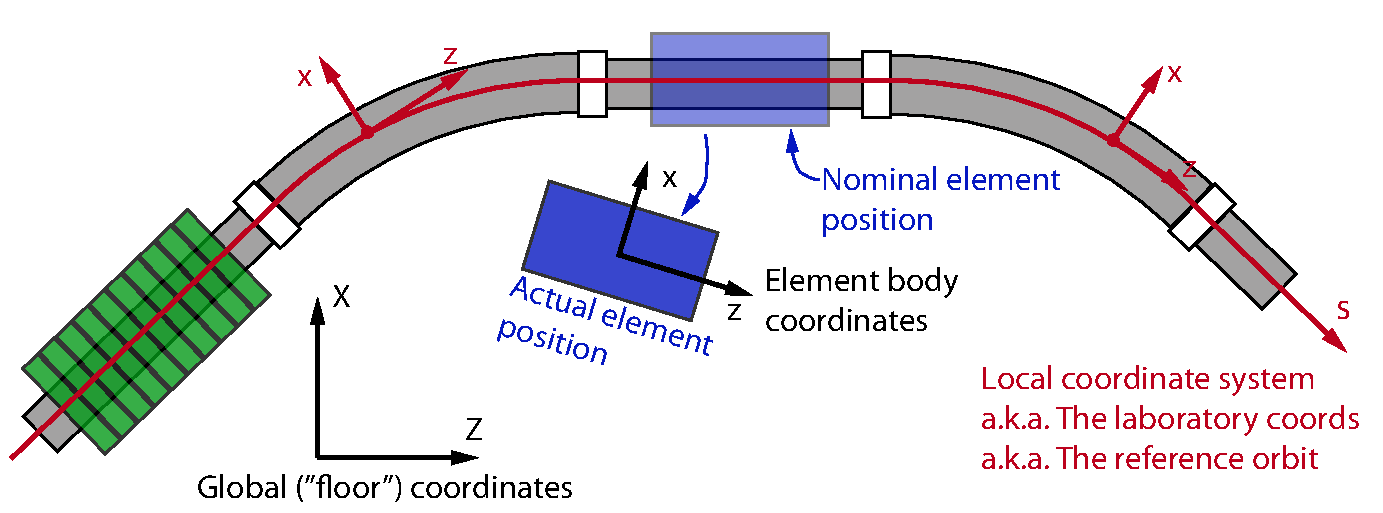
\includegraphics[width=5.0in]{coordinates.pdf}
  \caption[The three coordinate system used by \bmad.]
{The three coordinate systems used by \bmad: The \vn{global} (or ``\vn{floor}'') coordinate system
is independent of the accelerator.  The \vn{local} curvilinear coordinate system follows the bends
of the accelerator.  Each lattice element has \vn{element body} coordinates which, if the element is
not ``misaligned'' is the same as the \vn{local} coordinates. The $x=y=0$ curved line of the
laboratory coordinate system is known as the ``reference orbit''.}
  \label{f:coords}
\end{figure}

%-----------------------------------------------------------------------------
\section{Laboratory Coordinates and Reference Orbit}
\label{s:local.coords}

%-----------------------------------------------------------------------------
\subsection{The Reference Orbit}
\label{s:ref}
\index{reference orbit|hyperbf}
\index{laboratory coordinates|hyperbf}

\begin{figure}[tb]
  \centering
  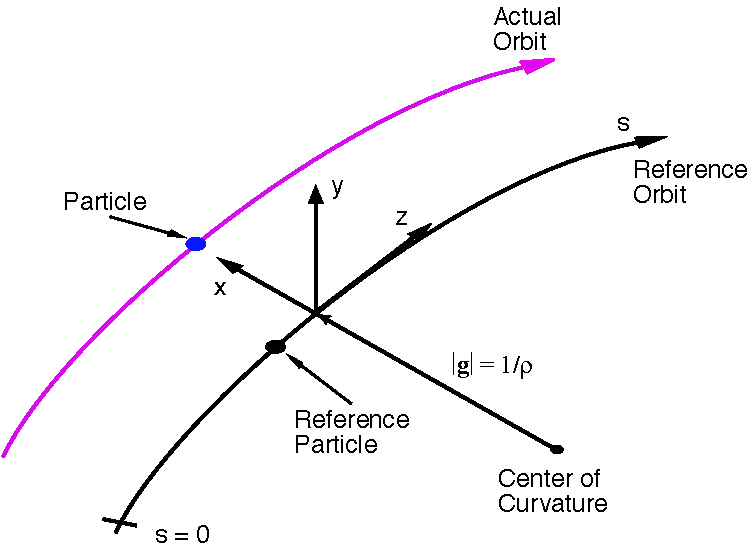
\includegraphics[width=6in]{local-coords.pdf}
  \caption[The local Reference System.]
{The local reference coordinate system. By construction, a particle's $z$ coordinate is zero.  This
is not to be confused with the phase space $z$ coordinate (\sref{s:phase.space}). The curvature
vector $\bfg$ lies in the $x$-$y$ plane and has a magnitude of $1/\rho$ where $\rho$ is the bending
radius. A) The $z$-axis will normally be parallel to the $s$-axis. B) For \vn{reversed} elements it
will be antiparallel. In both cases, the particle and reference particle are traveling in the
direction of greater $s$.}
  \label{f:local.coords}
\end{figure}

The \vn{local reference orbit} is the curved path used to define a coordinate system for describing
a particle's position as shown in \fig{f:local.coords}. The reference orbit is also used for
orientating lattice elements in space. At a given time $t$, a particle's position can be described
by a point $\calO$ on the reference orbit a distance $s$ relative to the reference orbit's zero
position plus a transverse $(x,y)$ offset. The point $\calO$ on the reference orbit is used as the
origin of the local $(x, y, z)$ coordinate system with the $z$--axis tangent to the reference
orbit. The $z$--axis will generally be pointing in the direction of increasing $s$
(\fig{f:local.coords}A) but, as discussed below, will point counter to $s$ for elements that are
\vn{reversed} (\fig{f:local.coords}B). The $x$ and $y$--axes are perpendicular to the reference
orbit and, by construction, the particle is always at $z = 0$. The coordinate system so constructed
is called the \vn{``local coordinate system''} or sometimes the \vn{``laboratory coordinate
system''} when there is need to distinguish it from the \vn{``element coordinate system''}
(\sref{s:coords.3}) which is attached to the physical element. There is a separate reference orbit
for each branch (\sref{s:branch.def}) of a lattice.

\index{x_offset}\index{y_offset}
\index{x_pitch}\index{y_pitch}\index{wiggler}
Notice that, in a \vn{wiggler}, the reference orbit, which is a straight line, does {\em not}
correspond to the orbit that any actual particle could travel. Typically the physical element is
centered with respect to the reference curve. However, by specifying offsets, pitches or a tilt (See
\sref{s:offset}), the physical element may be arbitrarily shifted with respect to its reference
curve. Shifting a physical magnet with respect to its reference curve generally means that the
reference curve does {\em not} correspond to the orbit that any actual particle could travel.

Do not confuse this reference orbit (which defines the local coordinate system) with the reference
orbit about which the transfer maps are calculated (\sref{s:twiss}). The former is fixed by the
lattice while the latter can be any arbitrary orbit.

%-----------------------------------------------------------------------------
\subsection{Element Entrance and Exit Coordinates}
\label{s:ent.exi}
\index{element coordinates}

%--------------------------------------

  \begin{figure}[tb]
  \centering
  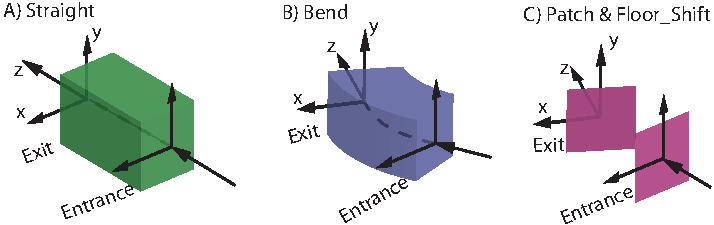
\includegraphics[width=5in]{element-coord-frame.pdf}
\caption[Lattice elements as LEGO blocks.]{Lattice elements can be imagined as ``LEGO blocks'' which
fit together to form the reference orbit along with the laboratory coordinate system. How elements
join together is determined in part by their entrance and exit coordinate frames. A) For
straight line elements the entrance and exit frames are colinear. B) For bends elements, the two
frames are rotated with respect to each other. C) For \vn{patch} and \vn{floor_shift} elements the
exit frame may be arbitrarily positioned with respect to the entrance frame.}
  \label{f:ele.coord.frame}
  \end{figure}

%--------------------------------------

\index{sbend}\index{rbend}
\index{crystal}\index{mirror}\index{entrance_end}
\index{exit_end}\index{patch}\index{floor_shift}
One way of thinking about the reference orbit and the laboratory coordinates is to imagine that each
element is like a LEGO block with an ``\vn{entrance}'' and an ``\vn{exit}'' coordinate frame as
illustrated in \fig{f:ele.coord.frame}\footnote
  {
Thanks to Dan Abell for this analogy.
  }. 
These coordinate frames are attached to the element. that is, things like electric and magnetic
fields, apertures, etc., are described with respect to the entrance and exit coordinates.  Thus, for
example, the \vn{e1} edge of a bend (\sref{s:bend}) is always at the \vn{entrance} face and the
\vn{e2} is always at the \vn{exit} face. Most elements have a ``straight'' geometry as shown in
\fig{f:ele.coord.frame}A. That is, the reference orbit through the element is a straight line
segment with the $x$ and $y$ axes always pointing in the same direction.  For a \vn{bend} element
(\sref{s:bend}), the reference orbit is a segment of a circular arc as shown in
\fig{f:ele.coord.frame}B. With the \vn{ref_tilt} parameter of a bend set to zero, the rotation axis
between the entrance and exit frames is parallel to the $y$-axis (\sref{s:global}). For \vn{patch}
(\sref{s:patch}), and \vn{floor_shift} (\sref{s:floor.ele}) elements, the exit face can can
arbitrarily oriented with respect to the entrance end. In this case, the reference orbit between the
entrance and exit faces is not defined.

%-----------------------------------------------------------------------------
\subsection{Reference Orbit and Laboratory Coordinates Construction}
\label{s:ref.construct}
\index{reference orbit!construction}
\index{upstream element end}\index{downstream element end}
\index{entrance element end}\index{exit element end}

%-----------------------------------------------------------------------------
\begin{figure}[tb]
  \centering
  \includegraphics[width=5in]{patch-between.pdf}
  \caption[Laboratory coordinates construction.]{A) The laboratory coordinates are constructed by
connecting the \vn{downstream} reference frame of one element with the \vn{upstream} reference frame
of the next element in the branch. Coordinates shown is for the mating of element \vn{A} to element
{B}.  B) Example with drift element \vn{dft} followed by a bend \vn{bnd}. Both elements are
unreversed. C) Similar to (B) but in this case element \vn{bnd} is reversed.  D) Similar to (C) but
in this case a reflection patch has been added in between \vn{dft} and \vn{bnd}.  In (B), (C), and
(D) the $(x,z)$ coordinates are drawn at the \vn{entrance} end of the elements. The $y$ coordinate
is always out of the page.}
  \label{f:patch.between}
\end{figure}
%-----------------------------------------------------------------------------

\index{root branch}
Assuming for the moment that there are no \vn{fiducial} elements present, the construction of the
reference orbit starts at the \vn{beginning_ele} element (\sref{s:begin.ele}) at the start of a
branch. If the branch is a \vn{root} branch (\sref{s:lattice.def}), The orientation of the beginning
element within the global coordinate system (\sref{s:coords.3}) can be set via the appropriate
positioning statements (\sref{s:beginning}). If the branch is not a \vn{root} branch, the position
of the beginning element is determined by the position of the \vn{fork} or \vn{photon_fork} element
from which the branch forks from. Unless set otherwise in the lattice file, $s = 0$ at the
\vn{beginning_ele} element.

If there are \vn{fiducial} elements, the laboratory coordinates are constructed beginning at these
elements.

Once the beginning element in a branch is positioned, succeeding elements are concatenated together
to form the laboratory coordinates. All elements have an ``\vn{upstream}'' and a ``\vn{downstream}''
end as shown in \fig{f:patch.between}A. The \vn{downstream} end of an element is always farther (at
greater $s$) from the beginning element than the \vn{upstream} end of the element.  Particles travel
in the $+s$ direction, so particles will enter an element at the upstream end and exit at the
downstream end.

Normally, the \vn{upstream} end is the element's \vn{entrance} end (\fig{f:ele.coord.frame}) and the
\vn{downstream} end is the element's \vn{exit} exit. This corresponds to particles entering at the
entrance end and exiting the element at the exit end. However, if an element is reversed
(\sref{s:ele.reverse}), the element's \vn{exit} end will be \vn{upstream} end and the element's
\vn{entrance} end will be the \vn{downstream} end. That is, for a reversed element, particles will
enter at the element's \vn{exit} end and will exit at the \vn{entrance} end.

The procedure to connect elements together to form the laboratory coordinates is to mate the
downstream reference frame of the element with the upstream reference frame of the next element in
the branch so that, without misalignments, the $(x,y,z)$ axes coincide\footnote
  {
If there are misalignments, the \vn{entrance} and \vn{exit} frames will move with the element. However,
the \vn{upstream} and \vn{downstream} frames, along with the reference orbit and laboratory
coordinates, will not move.
  }. 
This is illustrated in \fig{f:patch.between}. \fig{f:patch.between}A shows the general situation
with the downstream frame of element \vn{A} mated to the upstream frame of element \vn{B}.
Figures~\ref{f:patch.between}B-C show branches constructed from the following lattice file:
\begin{example}
  DFT: drift, l = 2
  BND: sbend, l = 2, g = pi/12
  P: patch, x_pitch = pi          ! Reflection patch.
  B_line: line = (DFT, BND)       ! No reversal.
  C_line: line = (DFT, --BND)     ! Illegal. Do not use!
  D_line: line = (DFT, P, --BND)  ! Valid.
\end{example}
The $(x,z)$ coordinates are drawn at the entrance end of the elements and $z$ will always point
towards the element's exit end.  \fig{f:patch.between}B shows the branch constructed from
\vn{B_line} containing an unreversed drift named \vn{dft} connected to an unreversed bend named
\vn{bnd}. \fig{f:patch.between}C shows the branch constructed from \vn{C_line}. This is like
\vn{B_line} except here element \vn{bnd} is reversed. This gives an unphysical situation since a
particle traveling through \vn{dft} will ``fall off'' when it gets to the end.
\fig{f:patch.between}D shows the branch constructed from \vn{D_line}. Here a ``\vn{reflection}''
patch \vn{P} (\sref{s:reflect.patch}) has been added to get a plausible geometry. The patch rotates the
coordinate system around the $y$-axis by 180\Deg (leaving the $y$-axis invariant). It is always the
case that a reflection patch is needed between reversed and unreversed elements

Notes:
\begin{itemize}
\item
If the first element after the \vn{beginning_ele} element at the start of a branch is reversed, the
\vn{beginning_ele} element will be marked as reversed so that a reflection patch is not needed in
this circumstance.
\item
Irrespective of whether elements are reversed or not, the laboratory $(x,y,z)$ coordinate system
at all $s$-positions will always be a right-handed coordinate system.
\item
Care must be take when using reversed elements. For example, if the field of the \vn{bnd} element in
\vn{B_line} is appropriate for, say, electrons, that is, electrons will be bent in a clockwise
fashion going through \vn{bnd}, then an electron going through \vn{D_line} will be lost in the bend
(the $y$-axis and hence the field is in the same direction for both cases so electrons will still be
bent in a clockwise fashion but with \vn{D_line} a particle needs to be bent counterclockwise to get
through the bend). To get a particle through the bend, positrons must be used.
\item
A reflection patch that rotated the coordinates, for example, around the $x$-axis by 180\Deg (by
setting \vn{y_pitch} to \vn{pi}) would also produce a plausible geometry.
\end{itemize}

%-----------------------------------------------------------------------------

\begin{figure}[bt]
  \centering
  \includegraphics[width=5in]{patch-problem.pdf}
  \caption[The local reference coordinates in a \vn{patch} element.]
{The local reference coordinates in a \vn{patch} element. The \vn{patch} element, shown
schematically as an irregular quadrilateral, is sandwiched between elements \vn{ele_a} and
\vn{ele_b}. \vn{L} is the length of the \vn{patch}. In this example, the \vn{patch} has a finite
\vn{x_pitch}.}
  \label{f:patch.prob}
\end{figure}

%-----------------------------------------------------------------------------
%-----------------------------------------------------------------------------
\subsection{Patch Element Local Coordinates}
\label{s:patch.prob}
\index{patch}

Generally, if a particle is reasonably near the reference orbit, there is a one-to-one mapping
between the particle's position and $(x, y, s)$ coordinates. A \vn{patch} (\sref{s:patch}) elements
with a non-zero \vn{x_pitch} or non-zero \vn{y_pitch} breaks the one-to-one mapping. This is
illustrated in \fig{f:patch.prob}.  The \vn{patch} element, shown schematically as an, irregular
quadrilateral, is sandwiched between elements \vn{ele_a} and \vn{ele_b}. The local coordinate system
with origin at $\alpha$ are the coordinates at the end of \vn{ele_a}. The coordinates at the end of
the \vn{patch} has its origin labeled $\gamma$. By convention, the length of the patch \vn{L} is
taken to be the longitudinal distance from $\alpha$ to $\gamma$ with the \vn{patch}'s exit
coordinates defining the longitudinal direction. The ``beginning'' point of the \vn{patch} on the
reference orbit a distance \vn{L} from point $\gamma$ is labeled $\beta$ in the figure.

In the local $(x, y, s)$ coordinate system a particle at $\alpha$ will have some value $s = s_0$. A
particle at point $\beta$ will have the same value $s = s_0$ and a particle at $\gamma$ will have $s
= s_1 = s_0 + L$. A particle at point $r_a$ in \fig{f:patch.prob} illustrates the problem of
assigning $(x, y, s)$ coordinates to a given position. If the particle is considered to be within
the region of \vn{ele_a}, the particle's $s$ position will be $s_{a2}$ which is greater than the
value $s_0$ at the exit end of the element. This contradicts the expectation that particles within
\vn{ele_a} will have $s \le s_0$.  If, on the other hand, the particle is considered to be within
the \vn{patch} region, the particle's $s$ position will be $s_{a1}$ which is less than the value
$s_0$ at the entrance to the patch. This contradicts the expectation that a particles within the
\vn{patch} will have $s \ge s_0$.

To resolve this problem, \bmad considers a particle at position $r_a$ to be within the \vn{patch}
region. This means that there is, in theory, no lower limit to the $s$-position that a particle in
the \vn{patch} region can have. This also implies that there is a discontinuity in the $s$-position
of a particle crossing the exit face of \vn{ele1}. Typically, when particles are translated from the
exit face of one element to the exit face of the next, this \vn{patch} problem does not appear. It
only appears when the track between faces is considered.

Notice that a particle at position $r_b$ in \fig{f:patch.prob} can simultaneously be considered to
be in either \vn{ele_a} or the \vn{patch}. While this creates an ambiguity it does not complicate
tracking.

%-----------------------------------------------------------------------------
\section{Global Coordinates}
\label{s:global}
\index{global coordinates|hyperbf}

\begin{figure}[tb]
  \centering
  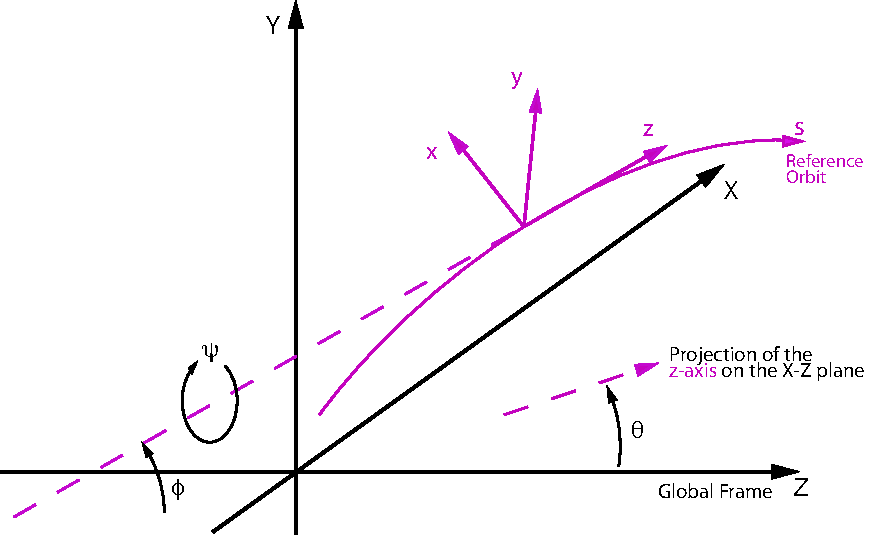
\includegraphics{global-coords.pdf}
  \caption[The Global Coordinate System]{
The local (reference) coordinate system (purple), which is a function of $s$ along the reference
orbit, is described in the global coordinate system (black) by a position $(X(s), Y(s), Z(s))$ and
and by angles $\theta(s)$, $\phi(s)$, and $\psi(s)$.
  }
  \label{f:global.coords}
\end{figure}

The Cartesian \vn{global} coordinate system, also called the `floor'' coordinate system, is the
coordinate system ``attached to the earth'' that is used to describe the local coordinate
system. Following the \mad\ convention, the \vn{global} coordinate axis are labeled $(X, Y,
Z)$. Conventionally, $Y$ is the ``vertical'' coordinate and $(X, Z)$ are the ``horizontal''
coordinates. To describe how the local coordinate system is oriented within the global coordinate
system, each point on the $s$-axis of the local coordinate system is characterized by its $(X, Y,
Z)$ position and by three angles $\theta(s)$, $\phi(s)$, and $\psi(s)$ that describe the orientation
of the local coordinate axes as shown in \fig{f:global.coords}. These three angles are defined as
follows:
\begin{description}
%
\item[$\theta(s)$ Azimuth (yaw) angle:] 
Angle in the $(X, Z)$ plane between the $Z$--axis and the projection of the $z$--axis onto the $(X,
Z)$ plane. Corresponds to the \vn{x_pitch} element attribute (\sref{s:offset}). A positive angle of
$\theta = \pi/2$ corresponds to the projected $z$--axis pointing in the positive $X$ direction.
%
\item[$\phi(s)$ Pitch (elevation) angle:] 
Angle between the $z$--axis and the $(X,Z)$ plane. Corresponds to the \vn{y_pitch} element attribute
(\sref{s:offset}). A positive angle of $\phi = \pi/2$ corresponds to the $z$--axis pointing in the
positive $Y$ direction.
%
\item[$\psi(s)$ Roll angle:] 
Angle of the $x$--axis with respect to the line formed by the intersection of the $(X, Z)$ plane
with the $(x, y)$ plane. Corresponds to the \vn{tilt} element attribute (\sref{s:offset}). A
positive $\psi$ forms a right--handed screw with the $z$--axis.
\end{description}

\index{beginning statement}
\index{reference orbit!origin in global coordinates}
\index{global coordinates!reference orbit origin}
By default, at $s = 0$, the reference orbit's origin coincides with the $(X, Y, Z)$ origin and the
$x$, $y$, and $z$ axes correspond to the $X$, $Y$, and $Z$ axes respectively. If the lattice has no
vertical bends (the \vn{ref_tilt} parameter (\sref{s:bend}) of all bends are zero), the $y$--axis
will always be in the vertical $Y$ direction and the $x$--axis will lie in the horizontal $(X,Z)$
plane. In this case, $\theta$ decreases as one follows the reference orbit when going through a
horizontal bend with a positive bending angle. This corresponds to $x$ pointing radially
outward. Without any vertical bends, the $Y$ and $y$ axes will coincide, and $\phi$ and $\psi$ will
both be zero. The \vn{beginning} statement (\sref{s:beginning}) in a lattice file can be use to
override these defaults.

\index{MAD}
Following \mad, the global position of an element is characterized by a vector $\bfV$
\begin{equation}
  \bfV = 
  \begin{pmatrix}
    X \\ Y \\ Z 
  \end{pmatrix}
\end{equation}
The orientation of an element is described by a unitary rotation matrix $\bfW$. The column vectors
of $\bfW$ are the unit vectors spanning the local coordinate axes in the order $(x, y, z)$. $\bfW$
can be expressed in terms of the orientation angles $\theta$, $\phi$, and $\psi$ via the formula
\begin{align}
  \bfW &= \bfR_{y}(\theta) \; \bfR_{-x}(\phi) \; \bfR_{z}(\psi) 
  \label{wwww} \\
  &= \begin{pmatrix}
    \cos\theta \cos\psi - \sin\theta \sin\phi \sin\psi & -\cos\theta \sin\psi - \sin\theta \sin\phi \cos\psi & 
                                                                                          \sin\theta \cos\phi \\
    \cos\phi \sin\psi & \cos\phi \cos\psi & \sin\phi \\
   -\cos\theta \sin\phi \sin\psi - \sin\theta \cos\psi & \sin\theta \sin\psi - \cos\theta \sin\phi \cos\psi & 
                                                                                          \cos\theta \cos\phi 
  \end{pmatrix}
  \nonumber
\end{align}
where
\begin{equation}
  \bfR_{y}(\theta) = 
  \begin{pmatrix}
    \cos\theta  & 0 & \sin\theta \\
    0           & 1 & 0          \\
    -\sin\theta & 0 & \cos\theta 
  \end{pmatrix}, \quad
  \bfR_{-x}(\phi) = 
  \begin{pmatrix}
    1 & 0 & 0                \\
    0 & \cos\phi  & \sin\phi \\
    0 & -\sin\phi & \cos\phi 
  \end{pmatrix}, \quad
  \bfR_{z}(\psi) = 
  \begin{pmatrix}
    \cos\psi & -\sin\psi & 0 \\
    \sin\psi &  \cos\psi & 0 \\
    0        &  0        & 1                
  \end{pmatrix}
  \label{wtt0t}
\end{equation}
Notice that $\bfR_{-x}(\phi)$, for positive $\phi$, represents a rotation around the negative
$x$-axis. Also notice that these are Tait-Bryan angles and not Euler angles.

An alternative representation of the $\bfW$ matrix (or any other rotation matrix) is to specify the
axis $\Bf u$ (normalized to 1) and angle of rotation $\beta$
\begin{equation}
  \bfW = \begin{pmatrix}
    \cos \beta + u_x^2 \left(1 - \cos \beta \right) & 
    u_x \, u_y \left(1 - \cos \beta \right) - u_z \sin \beta & 
    u_x \, u_z \left(1 - \cos \beta \right) + u_y \sin \beta \\ 
    u_y \, u_x \left(1 - \cos \beta \right) + u_z \sin \beta & 
    \cos \beta + u_y^2\left(1 - \cos \beta \right) & 
    u_y \, u_z \left(1 - \cos \beta \right) - u_x \sin \beta \\ 
    u_z \, u_x \left(1 - \cos \beta \right) - u_y \sin \beta & 
    u_z \, u_y \left(1 - \cos \beta \right) + u_x \sin \beta & 
    \cos \beta + u_z^2\left(1 - \cos \beta \right)
  \end{pmatrix}
  \label{wctux2}
\end{equation}

%-----------------------------------------------------------------------------
\subsection{Lattice Element Positioning}
\label{s:ele.pos}

\index{MAD}
\bmad, again following \mad, computes $\bfV$ and $\bfW$ by starting at the first element of the
lattice and iteratively using the equations
\begin{align}
  \bfV_i &= \bfW_{i-1} \; \bfL_i + \bfV_{i-1}, 
    \label{vwlv} \\
  \bfW_i &= \bfW_{i-1} \; \bfS_i
    \label{wws}
\end{align}
$\bfL_i$ is the displacement vector for the $i$\Th element and matrix $\bfS_i$ is the rotation of
the local reference system of the exit end with respect to the entrance end. For clarity, the
subscript $i$ in the equations below will be dripped. For all elements whose reference orbit through
them is a straight line, the corresponding $\bfL$ and $\bfS$ are
\begin{equation}
  \bfL = 
  \begin{pmatrix}
      0 \\ 0 \\ L
  \end{pmatrix},
  \quad
  \bfS = 
  \begin{pmatrix}
      1 & 0 & 0 \\ 
      0 & 1 & 0 \\
      0 & 0 & 1
  \end{pmatrix},
  \label{l00l}
\end{equation}
Where $L$ is the length of the element. 

%-----------------------------------------------------------------------

\begin{figure}
\centering \includegraphics{tilt-bend.pdf} 
\caption[Orientation of a Bend.] 
  {
A) Rotation axes (bold arrows) for four different \vn{ref_tilt} angles of $\theta_t$ = 0, $\pm
\pi/2$, and $\pi$. $(x_0, y_0, z_0)$ are the local coordinates at the entrance end of the bend with
the $z_0$ axis being directed into the page. Any rotation axis will be displaced by a distance of
the bend radius \vn{rho} from the origin. B) The $(x, y, z)$ coordinates at the exit end of the bend
for the same four \vn{ref_tilt} angles. In this case the bend angle is taken to be $\pi/2$.
  }
  \label{f:tilt.bend}
\end{figure}

%-----------------------------------------------------------------------

\index{rbend}\index{sbend}
\index{rho}\index{tilt}\index{angle}
For a \vn{bend}, the axis of rotation is dependent upon the bend's \vn{ref_tilt} angle
(\sref{s:offset}) as shown in \fig{f:tilt.bend}A. The axis of rotation points in the negative $y_0$
direction for \vn{ref_tilt} = 0 and is offset by the bend radius \vn{rho}. Here $(x_0, y_0, z_0)$
are the local coordinates at the entrance end of the bend with the $z_0$ axis being directed into
the page in the figure.  For a non-zero \vn{ref_tilt}, the rotation axis is itself rotated about the
$z_0$ axis by the value of \vn{ref_tilt}. \fig{f:tilt.bend}B shows the exit coordinates for four
different values of \vn{ref_tilt} and for a bend angle \vn{angle} of $\pi/2$.  Notice that for a
bend in the horizontal $X-Z$ plane, a positive bend \vn{angle} will result in a decreasing azimuth
angle $\theta$.

For a bend, $\bfS$ is given using \Eq{wctux2} with 
\begin{align}
  \Bf u &= (-\sin\theta_t, -\cos\theta_t, 0) \CRNO
  \beta &= \alpha_b
  \label{ustt}
\end{align}
where $\theta_t$ is the \vn{ref_tilt} angle. The $\bfL$ vector for a \vn{bend} is given by 
\begin{equation}
  \bfL = \bfR_{z}(\theta_t) \; \bftilde L, \quad
  \bftilde L = 
  \begin{pmatrix}
    \rho (\cos\alpha_b - 1) \\ 0 \\ \rho \, \sin\alpha_b
  \end{pmatrix}
  \label{lrztt}
\end{equation}
where $\alpha_b$ is the bend \vn{angle} (\sref{s:bend}) and $\rho$ being the bend radius
(\vn{rho}). Notice that since $\Bf u$ is perpendicular to $z$, the curvilinear reference coordinate
system has no ``torsion''. That is, it is a Frenet-Serret coordinate system.

Note: An alternative equation for \vn{\bfS} for a bend is
 \begin{equation}
  \bfS = \bfR_{z}(\theta_t) \; \bfR_{y}(-\alpha_b) \; \bfR_{z}(-\theta_t)
  \label{srrr}
\end{equation}

The bend transformation above is so constructed that the transformation is equivalent to rotating
the local coordinate system around an axis that is perpendicular to the plane of the bend. This
rotation axis is invariant under the bend transformation. For example, for $\theta_t = 0$ (or $\pi$)
the $y$-axis is the rotation axis and the $y$-axis of the local coordinates before the bend will be
parallel to the $y$-axis of the local coordinates after the bend as shown in \fig{f:tilt.bend}. That
is, a lattice with only bends with $\theta_t = 0$ or $\pi$ will lie in the horizontal plane (this
assuming that the $y$-axis starts out pointing along the $Y$-axis as it does by default).  For
$\theta_t = \pm\pi/2$, the bend axis is the $x$-axis. A value of $\theta_t = +\pi/2$ represents a
downward pointing bend.

\begin{figure}
  \centering \includegraphics{mirror.pdf} 
\caption[Mirror and crystal geometry] {Mirror and crystal geometry.  The geometry shown here is
appropriate for a \vn{ref_tilt} angle of $\theta_t = 0$.  $\theta_g$ is the bend angle of the
incoming (entrance) ray, and $\alpha_b$ is the total bend angle of the reference trajectory. A)
Geometry for a mirror or a Bragg crystal. Point $\calO$ is the origin of both the local coordinates
just before and just after the reflection/diffraction. B) Geometry for a Laue crystal.  Point
$\calO_{out}$ is the origin of the coordinates just after diffraction is displaced from the origin
$\calO_{in}$ just before diffraction due to the finite thickness of the crystal. here the bend
angles are measured with respect to the line that is in the plane of the entrance and exit
coordinates and perpendicular to the surface. For Laue diffraction, the user has the option of using
the undiffracted beam (shown in red) as the reference trajectory.
  }  
  \label{f:mirror}
\end{figure}

%-----------------------------------------------------------------------------
\subsection{Position Transformation When Transforming Coordinates}
\label{s:pos.trans}

A point $\bfQ_g = (X, Y, Z)$ defined in the global coordinate system, when expressed in the
coordinate system defined by $(\bfV, \bfW)$ is
\begin{equation}
  \bfQ_{VW} = \bfW^{-1} \left( \bfQ_g - \bfV \right)
  \label{rwrv}
\end{equation}
This is essentially the inverse of \Eq{vwlv}. That is, vectors propagate inversely to the
propagation of the coordinate system.

Using \Eq{rwrv} with \Eqs{vwlv}, and \eq{wws}, the transformation of a particle's position $\bfq =
(x,y,z)$ and momentum $\bfP = (P_x, P_y, P_z)$ when the coordinate frame is transformed from frame
$(\bfV_{i-1}, \bfW_{i-1})$ to frame $(\bfV_i, \bfW_i)$ is
\begin{align}
  \bfq_i &= \bfS_i^{-1} \, \left( \bfq_{i-1} - \bfL_i \right), 
    \label{rwlr} \\
  \bfP_i &= \bfS_i^{-1} \, \bfP_{i-1}
    \label{pps}
\end{align}

Notice that since $\bfS$ (and $\bfW$) is the product of orthogonal rotation matrices, $\bfS$ is
itself orthogonal and its inverse is just the transpose
\begin{equation}
  \bfS^{-1} = \bfS^T
\end{equation}

%-----------------------------------------------------------------------------
\subsection{Crystal and Mirror Element Coordinate Transformation}
\label{s:mirror.coords}

\index{crystal}\index{mirror}\index{ref_tilt}
A \vn{crystal} element (\sref{s:mirror}) diffracts photons and a \vn{mirror} element
(\sref{s:mirror}) reflects them. For a crystal setup for Bragg diffraction, and for a mirror, the
reference orbit is modeled as a zero length bend with $\bftilde L = (0, 0, 0)$, as shown in
\fig{f:mirror}A. Shown in the figure is the geometry appropriate for a \vn{ref_tilt} angle of
$\theta_t = 0$ (the rotation axis is here the $y$-axis). Since the mirror or crystal element is
modeled to be of zero length, the origin points (marked $\calO$ in the figure) of the entrance and
exit local coordinates are the same. For Laue diffraction, the only difference is that $\bftilde L$
is non-zero due to the finite thickness of the crystal as shown in \fig{f:mirror}B. This results in
a separation between the entrance coordinate origin $\calO_{in}$ and the exit coordinate origin
$\calO_{out}$.

In all cases, the total bending angle is
\begin{align}
  \alpha_b &= \text{bragg_angle_in} + \text{bragg_angle_out} &&\text{! Crystal, graze_angle_in} = 0 \CRNO
  \alpha_b &= \text{graze_angle_in} + \text{graze_angle_out} &&\text{! Crystal, graze_angle_in} \ne 0 \CRNO
  \alpha_b &= 2 \, \text{graze_angle}                        &&\text{! Mirror}
  \label{agg}
\end{align}
With a mirror or Bragg diffraction, the bend angles are measured with respect to the surface
plane. With Laue diffraction the bend angles are measured with respect to the line in the bend plane
perpendicular to the surface.

For Laue diffraction, the user has the option of using the undiffracted beam (shown in red) as the
reference trajectory.

The orientation of the exit coordinates (the local coordinates after the reflection) are only
affected by the element's \vn{ref_tilt} and bend angle parameters and is independent of all other
parameters such as the radius of curvature of the surface, etc. The local $z$-axis of the entrance
coordinates along with the $z$-axis of the exit coordinates define a plane which is called the
element's \vn{bend plane}.  For a mirror, the graze angle is a parameter supplied by the user. For a
crystal, the Bragg angles are calculated so that the reference trajectory is in the middle of the
Darwin curve. Calculation of the Bragg angles for a crystal is given in
Section~\sref{s:crystal.ref}.

%-----------------------------------------------------------------------------
\subsection{Patch and Floor_Shift Elements Entrance to Exit Transformation}
\label{s:patch.coords}

\index{patch!coordinate transformation}\index{floor_shift!coordinate transformation}
For \vn{patch} (\sref{s:patch}) and \vn{floor_shift} (\sref{s:floor.ele}) elements, the shift in the
exit end reference coordinates is given by \Eqs{vwlv} and \eq{wws} with
\begin{align}
  \bfL &= 
    \begin{pmatrix} 
      \text{x_offset} \\ \text{y_offset} \\ \text{z_offset} 
    \end{pmatrix}
    \CRNO
  \bfS &= \bfR_{y} (\text{x_pitch}) \; \bfR_{-x} (\text{y_pitch}) \; \bfR_{z} (\text{tilt})
  \label{swww}
\end{align}

The difference here between \vn{patch} and \vn{floor_shift} elements is that, with a \vn{patch}
element, the shift is relative to the exit end of the previous element while, for a \vn{floor_shift}
element, the shift is relative to the reference point on the origin element specified by the
\vn{origin_ele} parameter of the \vn{floor_shift}.

%-----------------------------------------------------------------------------
\subsection{Fiducial and Girder Elements Origin Shift Transformation}
\label{s:girder.coords}

\index{girder}\index{fiducial}
For \vn{fiducial} and \vn{girder} elements, the alignment of the
reference coordinates with respect to ``\vn{origin}'' coordinates is
analogous to \Eqs{swww}. Explicitly:
\begin{align}
  \bfL &= 
    \begin{pmatrix} 
      \text{dx_origin} \\ \text{dy_origin} \\ \text{dz_origin}
    \end{pmatrix}
    \CRNO
  \bfS &= \bfR_{y} (\text{dtheta_origin}) \; \bfR_{-x} (\text{dphi_origin}) \; \bfR_{z} (\text{dpsi_origin})
\end{align}

%-----------------------------------------------------------------------------
\subsection{Reflection Patch}
\label{s:reflect.patch}
\index{patch!reflection}

A \vn{Patch} (or a series of patches) that reflects the direction of the \vn{z}-axis is called a
\vn{reflection} \vn{patch}. By ``reflected direction'' it is meant that the dot product $\Bf z_1
\cdot \Bf z_2$ is negative where $\Bf z_1$ is the $z$-axis vector at the \vn{entrance} face and $\Bf
z_2$ is the $z$-axis vector at the \vn{exit} face. This condition is equivalent to the condition
that the associated $\bfS$ matrix (see \Eq{swww}) satisfy:
\begin{equation}
  S(3,3) < 0
  \label{s330}
\end{equation}
Using \Eq{swww} gives, after some simple algebra, this condition is equivalent to
\begin{equation}
  \cos(\text{x_pitch}) \, \cos(\text{y_pitch}) < 0
\end{equation}
When there are a series of patches, The transformations of all the patches are concatenated together
to form an effective $\bfS$ which can then be used with \Eq{s330}.

%\begin{figure}[!b]
%  \centering
%  \includegraphics[width=5.0in]{edge-track.pdf}
%  \caption[]
%{
%}
%  \label{f:edge.track}
%\end{figure}

%-----------------------------------------------------------------------------
\section{Transformation Between Laboratory and Element Body Coordinates}
\label{s:lab.body.transform}
\index{laboratory coordinates}
\index{element body coordinates|hyperbf}

The \vn{element body} coordinates are the coordinate system attached to an element. Without any
misalignments, where \vn{``misalignments''} are here defined to be any offset, pitch or tilt
(\sref{s:offset}), the \vn{laboratory} coordinates (\sref{s:ref}) and \vn{element body} coordinates
are the same. With misalignments, the transformation between \vn{laboratory} and \vn{element body}
coordinates depends upon whether the local coordinate system is straight (\sref{s:straight.mis}) or
bent (\sref{s:bend.mis}).

When tracking a particle through an element, the particle starts at the \vn{nominal}
(\sref{s:coords.3}) upstream end of the element with the particle's position expressed in laboratory
coordinates. Tracking from the the nominal upstream end to the actual upstream face of the element
involves first transforming to element body coordinates (with $s = 0$ in the equations below) and
then propagating the particle as in a field free drift space from the particle's starting position
to the actual element face. Depending upon the element's orientation, this tracking may involve
tracking backwards. Similarly, after a particle has been tracked through the physical element to the
actual downstream face, the tracking to the nominal downstream end involves transforming to
laboratory coordinates (using $s = L$ in the equations below) and then propagating the particle as
in a field free drift space to the nominal downstream edge.

%-----------------------------------------------------------------------------
\subsection{Straight Element Misalignment Transformation}
\label{s:straight.mis}

For straight line elements, given a laboratory coordinate frame $\Lambda_s$ with origin a distance
$s$ from the beginning of the element, misalignments will shift the coordinates to a new reference
frame denoted $E_s$. Since misalignments are defined with respect to the middle of the element, the
transformation between $\Lambda_s$ and $E_s$ is a three step process:
\begin{equation}
  \Lambda_s \longrightarrow \Lambda_\text{mid} 
  \longrightarrow E_\text{mid} \longrightarrow E_s
  \label{llee}
\end{equation}
where $\Lambda_\text{mid}$ and $E_\text{mid}$ are the laboratory and element reference frames at the
center of the element.

The first and last transformations from $\Lambda_s$ to $\Lambda_\text{mid}$ and from $E_\text{mid}$
to $E_s$ use \Eqs{vwlv}, \eq{wws}, and \eq{l00l} with the replacement $L \rightarrow L/2 - s$ for
the first transformation and $L \rightarrow s - L/2$ for the third transformation. The middle
transformation, by definition of the offset, pitch and tilt parameters is
\begin{align}
  \bfL &= 
    \begin{pmatrix} 
      \text{x_offset} \\ \text{y_offset} \\ \text{z_offset} 
    \end{pmatrix}
    \CRNO
  \bfS &= \bfR_{y} (\text{x_pitch}) \; \bfR_{-x} (\text{y_pitch}) \; \bfR_{z} (\text{tilt})
  \label{swww2}
\end{align}

Notice that with this definition of how elements are misaligned, the position of the center of a
non-bend misaligned element depends only on the offsets, and is independent of the pitches and tilt.

%-----------------------------------------------------------------------------
\subsection{Bend Element Misalignment Transformation}
\label{s:bend.mis}

\index{rbend!coordinate transformation}\index{sbend!coordinate transformation}
\index{roll!coordinate transformation}\index{tilt!coordinate transformation}
For \vn{rbend} and \vn{sbend} elements there is no \vn{tilt} attribute.  Rather, there is the
\vn{roll} attribute and a \vn{ref_tilt} attribute. The latter affects both the reference orbit and
the bend position (\sref{s:bend.orient}). Furthermore, \vn{ref_tilt} is calculated with respect to
the coordinates at the beginning of the bend while, like straight elements, \vn{roll}, offsets, and
pitches are calculated with respect to the center of the bend. The different reference frame used
for \vn{ref_tilt} versus everything else means that five transformations are needed to get from the
laboratory frame to the element body frame (see \Eq{llee}). Symbolically:
\begin{equation}
  \Lambda_s \longrightarrow \Lambda_\text{mid} 
  \longrightarrow \Omega_\text{mid} \longrightarrow \Omega_0
  \longrightarrow E_0 \longrightarrow E_s
\end{equation}

The first transformation, $\Lambda_s$ to $\Lambda_\text{mid}$, from laboratory coordinates at a
distance $s$ from the beginning of the element to laboratory coordinates at the center the bend is a
rotation around the center of curvature of the bend and is given by \Eqs{vwlv} and \eq{wws} with
\Eqs{ustt} and \eq{lrztt} with the substitution $\alpha_b \rightarrow (L/2 - s)/\rho$.

The second transformation $\Lambda_\text{mid}$ to $\Omega_\text{mid}$ at the center of the element
adds in the misalignments (Note that the coordinate frame $\Omega_\text{mid}$ is neither a
laboratory frame or an element frame so hence the use of a different symbol $\Omega$). Explicitly,
the $\Lambda_\text{mid} \longrightarrow \Omega_\text{mid}$ transformation is
\begin{align}
  \bfL &= \bfL_\text{off} + 
    \left[ \bfR_z(\text{roll}) - \Bf1 \right] \; \bfR_z(\theta_t) \; \bfR_{y}(\alpha_b/2) \; \bfL_c \CRNO
  \bfS &= \bfR_{y}(\text{x_pitch}) \; \bfR_{-x}(\text{y_pitch}) \; \bfR_z(\text{roll})
  \label{lcmis}
\end{align}
where
\begin{equation}
  \bfL_c = 
    \begin{pmatrix}
      \rho (\cos(\alpha_b/2) - 1) \\ 0 \\ \rho \, \sin(\alpha_b/2)
    \end{pmatrix}
  , \qquad
  \bfL_\text{off} = 
    \begin{pmatrix} 
      \text{x_offset} \\ \text{y_offset} \\ \text{z_offset} 
    \end{pmatrix}
\end{equation}
The reason why $\bfL$ has a different form from straight line elements is due to the fact that the
axis of rotation for a \vn{roll} is displaced from the $z$-axis of the coordinate system at the
center of the bend (see \fig{f:roll}).

The third transformation from $\Omega_\text{mid}$ to $\Omega_0$ is like the first transformation and
rotates from the center of the bend to the beginning. Again \Eqs{ustt} and \eq{lrztt} are used with
the substitution $\alpha_b \rightarrow -L/2\rho$.

The fourth transformation $\Omega_0$ to $E_0$ tilts the reference frame by an amount \vn{ref_tilt}:
\begin{equation}
  \bfL = 0, \quad
  \bfS = \bfR_{z}(\theta_t)
  \label{l0sr}
\end{equation}

The fifth and final transformation, $E_0$ to $E_s$, like the first and third, rotates around the
center of the bend but in this case, since we are dealing with element coordinates, the
\vn{ref_tilt} is ignored.  That is, \Eqs{ustt} and \eq{lrztt} are used with the substitutions
$\theta_t \rightarrow 0$ and $\alpha_b \rightarrow L/\rho$.

Notice that with this definition of how elements are misaligned, the position of the center of a
misaligned element depends only on the offsets and \vn{roll}, and is independent of the pitches and
tilt. Also the orientation of an element depends only on the pitches roll, and ref_tilt, and is
independent of the offsets.

%-----------------------------------------------------------------------------
\section{Phase Space Coordinates}
\label{s:phase.coords}
\index{phase space coordinates|hyperbf}

%-----------------------------------------------------------------------------
\subsection{Reference Particle, Reference Energy, and Reference Time}
\label{s:ref.energy}
\index{reference particle|hyperbf}
\index{reference energy|hyperbf}
\index{reference time|hyperbf}

The \vn{reference energy} and \vn{reference time} are needed in evaluating the phase space
coordinates of charged particles (\sref{s:phase.space}).

All lattice elements, except for controller elements, have an associated \vn{reference energy}
energy.  The reference energy at the start of a lattice's \vn{root branch} (\sref{s:branch.def}) is
set in the lattice file by setting the reference momentum (\vn{p0c}) or total energy (\vn{E_tot})
using a \vn{parameter} (\sref{s:param}) or \vn{beginning} (\sref{s:beginning}) statement. For other
branches, the energy at the start of the branch is set using the appropriate line parameter
(\sref{s:beginning}) statement.

Note that the reference momentum \vn{p0c} is actually the reference momentum times the speed of light
so that the reference momentum has the same unit (eV) as the reference energy.

\index{custom!reference energy}\index{em_field!reference energy}
\index{hybrid!reference energy}\index{lcavity!reference energy}
\index{patch!reference energy}
For most elements, the reference energy is the same as the reference energy of the proceeding
element. The following elements are exceptions:
\begin{example}
  custom
  em_field
  hybrid
  lcavity
  patch
\end{example}
The reference energy of these elements is determined by tracking a particle (the ``\vn{reference
particle}'') through the element with the particle starting on the reference orbit and whose energy
is equal to the reference energy. The energy of the particle at the downstream end is the reference
energy of the element. Note: Tracking through an element to determine the reference energy is always
done with the element turned on independent of the setting of the element's \vn{is_on}
(\sref{s:is.on}) parameter. Reference energy tracking is also done ignoring any orientation attributes
(\sref{s:offset}) and errors like \vn{voltage_err}.

\index{wiggler!reference time}
Besides the reference energy, lattice elements have an associated \vn{reference time} which is
computed, for most elements, by the time-of-flight of the \vn{reference particle} assuming that the
reference particle is following the reference orbit. Exceptions are \vn{wiggler} elements which uses
the time-of-flight of the actual undulating trajectory. [Actually what is used in the computation of
the $z$ phase space coordinate (\Eq{zbctt}) is the sum of reference time deltas of the elements that
a particle has passed through. It is not possible to assign a unique reference time to an element
when particles are recirculating through elements as in a storage ring.]

%-----------------------------------------------------------------------------
\subsection{Charged Particle Phase Space Coordinates}
\label{s:phase.space}
\index{phase space coordinates|hyperbf}

\begin{figure}
\centering \includegraphics{canonical-z.pdf} \caption[Interpreting phase space $z$ at constant
velocity.]  {Interpreting phase space $z$ at constant velocity: A) The change in $z$ going through
an element of length $L_0$ is $L_0 - L_p$.  B) At constant time, $z$ is the longitudinal distance
between the reference particle and the particle.}  \label{f:canonical.z}
\end{figure}

For charged particles (more correctly, for everything but photons (\sref{s:photon.phase.space})),
\bmad uses the canonical phase space coordinates
\begin{equation}
  \Bf r(s) = (x, p_x, y, p_y, z, p_z)
\end{equation}
The longitudinal position $s$ is the independent variable instead of the time. $x$ and $y$, are the
transverse coordinates of the particle as shown in~\fig{f:local.coords}A. Note that $x$ and $y$ are
independent of the position of the reference particle.

The phase space momenta $p_x$ and $p_y$ are normalized by the reference (sometimes called the
design) momentum $P_0$
\begin{equation}
  p_x = \frac{P_x}{P_0}, \qquad
  p_y = \frac{P_y}{P_0}
  \label{ppp}
\end{equation}
where $P_x$ and $P_y$ are respectively the $x$ and $y$ momentums.

\index{lcavity}\index{rfcavity}
The phase space $z$ coordinate is 
\begin{align}
  z(s) &= -\beta(s) \, c \, (t(s) - t_0(s)) \CRNO
    &\equiv - \beta(s) \, c \, \Delta t(s)
  \label{zbctt}
\end{align}
$t(s)$ is the time at which the particle is at position $s$, $t_0(s)$ is the time at which the
reference particle is at position $s$, and $\beta$ is $v/c$ with $v$ being the particle velocity
(and not the reference velocity). The reference particle is, by definition, ``synchronized'' with
elements whose fields are oscillating and therefore the actual fields a particle will see when
traveling through such an element will depend upon the particle's phase space $z$. For example, the
energy change of a particle traveling through an \vn{lcavity} (\sref{s:lcav}) or \vn{rfcavity}
(\sref{s:rfcav}) element is $z$ dependent. Exception: With absolute time tracking (\sref{s:rf.time})
fields are tied to the absolute time and not $z$.

If the particle's velocity is constant, and is the same as the velocity of the reference particle
(for example, at high energy where $\beta = 1$ for all particles), then $\beta \, c \, t$ is just
the path length. In this case, the change in $z$ going through an element is
\begin{equation}
  \Delta z = L_0 - L_p
\end{equation}
where, as shown in \fig{f:canonical.z}A, $L_0$ is the path length of the reference particle (which
is just the length of the element) and $L_p$ is the path length of the particle in traversing the
element.  Another way of interpreting phase space $z$ is that, at constant $\beta$, and constant
time, $z$ is the longitudinal distance between the particle and the reference particle as shown in
\fig{f:canonical.z}B. with positive $z$ indicating that the particle is ahead of the reference
particle.

Do not confuse the phase space $z$ with the $z$ that is the particle's longitudinal coordinate in
the local reference frame as shown in \fig{f:local.coords}. By construction, this latter $z$ is
always zero.

Notice that if a particle gets an instantaneous longitudinal kick so that $\beta$ is discontinuous
then, from \Eq{zbctt}, phase space $z$ is discontinuous even though the particle itself does not
move in space. In general, from \Eq{zbctt}, The value of $z$ for a particle at $s_2$ is related to
the value of $z$ for the particle at $s_1$ by
\begin{equation}
  z_2 = \frac{\beta_2}{\beta_1} \, z_1 - 
  \beta_2 \, c \, (\Delta t_2 - \Delta t_1)
  \label{zbbzb}
\end{equation}
$\Delta t_2 - \Delta t_1$ can be interpreted as the difference in transit time, between the particle
and the reference particle, in going from $s_1$ to $s_2$.

The longitudinal phase space momentum $p_z$ is given by
\begin{equation}
  p_z = \frac{\Delta P}{P_0} \equiv \frac{P - P_0}{P_0}
  \label{ppppp}
\end{equation}
where $P$ is the momentum of the particle. For ultra--relativistic particles $p_z$ can be
approximated by
\begin{equation}
  p_z = \frac{\Delta E}{E_0}
\end{equation}
\index{lcavity}
where $E_0$ is the reference energy (energy here always refers to the total energy) and $\Delta E =
E - E_0$ is the deviation of the particle's energy from the reference energy. For an \vn{Lcavity}
element (\sref{s:lcav}) the reference momentum is {\it not} constant so the tracking for an
\vn{Lcavity} is not canonical.

\index{phase space coordinates!MAD convention}
\index{MAD!phase space convention}
\mad uses a different coordinate system where $(z, p_z)$ is replaced by $(-c\Delta t, p_t)$ where
$p_t \equiv \Delta E / P_0 c$. For highly relativistic particles the two coordinate systems are
identical.

\index{paraxial approximation}
\index{bmad_standard!tracking method}
The relationship, between the phase space momenta and the slopes $x' \equiv dx/ds$ and $y' \equiv dy/ds$
is
\begin{align}
  x' &= \frac{p_x}{\sqrt{(1 + p_z)^2 - p_x^2 - p_y^2}} \, (1 + g x) \\
  y' &= \frac{p_y}{\sqrt{(1 + p_z)^2 - p_x^2 - p_y^2}} \, (1 + g x) 
  \label{xpa1p}
\end{align}
$g = 1/\rho$ is the curvature function with $\rho$ being the radius of curvature of the reference
orbit and it has been assumed that the bending is in the $x$--$z$ plane.

With the paraxial approximation, and in the relativistic limit, the change in $z$ with position is
\begin{equation}
  \frac{dz}{ds} = -g \, x - \frac{1}{2} (x'^2 + y'^2)
\end{equation}
This shows that in a linac, without any bends, the $z$ of a particle always decreases.

A particle can also have a spin. The spin is characterized by the spinor $\Psi = \left( \psi_{1},
\psi_{2} \right)^{T}$ where $\psi_{1,2}$ are complex numbers (\sref{s:spin.dyn}).

%-----------------------------------------------------------------------------
\subsection{Time-based Phase Space Coordinates}
\label{s:time.phase.space}
\index{time!phase space coordinates|hyperbf}

Some specialized routines (for example, time Runge Kutta tracking) use the time $t$ as the
independent variable for charged particle tracking. This is useful when particles can reverse
direction since the normal $z$ based tracking cannot handle this. Direction reversal can happen, for
example, with low energy ``dark current'' electrons that are generated at the walls of the vacuum
chamber.

When the tracking is time based the phase space coordinates are:
\begin{equation}
  (x, c \, p_x, y, c \, p_y, z, c \, p_s)
\end{equation}
The positions $x$, $y$, and $z$ are the same as with phase space coordinates
(\sref{s:phase.space}). The momenta are defined as
\begin{align}
c p_x &\equiv m c^2 \gamma \beta_x \CRNO
c p_y &\equiv m c^2 \gamma \beta_y \\
c p_s &\equiv m c^2 \gamma \beta_s, \nonumber
\end{align}
and internally are stored in units of eV.

%-----------------------------------------------------------------------------
\subsection{Photon Phase Space Coordinates}
\label{s:photon.phase.space}
\index{photon!phase space coordinates|hyperbf}

The phase space coordinates discussed above implicitly assume that
particles are traveling longitudinally in only one direction. That is,
the sign of the $s$ component of the momentum cannot be determined
from the phase space coordinates. This is generally fine for tracking
high energy beams of charged particles but for photon tracking this
would oftentimes be problematical. For photons, therefore, a different
phase space is used:
\begin{equation}
  (x, \beta_x, y, \beta_y, z, \beta_z)
  \label{xbybzb}
\end{equation}
Here $(\beta_x, \beta_y, \beta_z)$ is the normalized photon velocity with
\begin{equation}
  \beta_x^2 + \beta_y^2 + \beta_z^2 = 1 
  \label{bbb1}
\end{equation}
and $(x, y, z)$ are the reference orbit coordinates with $z$ being the
distance from the start of the lattice element the photon is in.

In \bmad, the information associated with a photon include its phase
space coordinates and time along with the photon energy and four
parameters $E_x, \phi_x$, and $E_y, \phi_y$ specifying the intensity
and phase of the field along the $x$ and $y$ axes transverse to the
direction of propagation.  the field in the vicinity of the photon is
\begin{align}
  E_x (\Bf r, t) &\sim E_x \, e^{i (k \, (z - z_0) - \omega \, (t - t_\REF) + \phi_x)} \CRNO
  E_y (\Bf r, t) &\sim E_y \, e^{i (k \, (z - z_0) - \omega \, (t - t_\REF) + \phi_y)} 
  \label{ertee}
\end{align}
where $z_0$ is the photon $z$ position and and $t_\REF$ is the reference time.

The normalization between field and intensity is dependent upon the
particular parameters of any given simulation and so must be
determined by the program using \bmad.


\chapter{Electromagnetic Fields}

%-----------------------------------------------------------------
\section{Magnetostatic Multipole Fields}
\label{s:mag.field}
\index{magnetic fields|hyperbf}

\index{MAD}
Start with the assumption that the local magnetic field has no longitudinal component
(obviously this assumption does not work with, say, a solenoid).  Following \mad, ignoring
skew fields for the moment, the vertical magnetic field along the $y = 0$ axis is expanded
in a Taylor series
\begin{equation}
  B_y(x, 0) = \sum_n B_n \, \frac{x^n}{n!}
  \label{byx0b}
\end{equation}
Assuming that the reference orbit is locally straight (there are correction terms if the
reference orbit is curved (\sref{s:field.exact})), the field is
\begin{alignat}{5}
  B_x &=           &&B_1 y \plus         &&B_2 \, xy       
                   && \plus && \frac{1}{6} B_3 (3x^2 y - y^3) \plus \ldots \CRNO
  B_y &= B_0 \plus &&B_1 x + \frac{1}{2} &&B_2 (x^2 - y^2) 
                   && \plus && \frac{1}{6} B_3 (x^3 - 3x y^2) \plus \ldots
  \label{bbb}
\end{alignat}
The relation between the field $B_n$ and the normalized field $K_n$ is:
\index{multipole!KnL, Tn|hyperbf}
\begin{equation}
  K_n \equiv \frac{q \, B_n}{P_0}
  \label{kqlbp}
\end{equation}
where $q$ is the charge of the reference particle (in units of the elementary charge), and $P_0$ is
the reference momentum (in units of eV/c).  Note that $P_0/q$ is sometimes written as $B\rho$. This
is just an old notation where $\rho$ is the bending radius of a particle with the reference energy
in a field of strength $B$. Notice that $P_0$ is the local reference momentum at the element which
may not be the same as the reference energy at the beginning of the lattice if there are
\vn{lcavity} elements (\sref{s:lcav}) present.

The kicks $\Delta p_x$ and $\Delta p_y$ that a particle experiences going through a multipole field
is
\begin{alignat}{5}
  \Delta p_x & = \frac{-q \, L \, B_y}{P_0} \label{pqlbp1} \\
             & = -K_0 L \;-\; 
             && K_1 L \, x \plus 
             \frac{1}{2} && K_2 L (y^2 - x^2) && \plus 
             && \frac{1}{6} K_3 L (3x y^2 - x^3) \plus \ldots 
             \nonumber \\
  \Delta p_y & = \frac{q \, L \, B_x}{P_0} \label{pqlbp2} \\
             & =     
             && K_1 L \, y \plus 
             && K_2 L \, xy && \plus 
             && \frac{1}{6} K_3L (3x^2 y - y^3) \plus \ldots \nonumber 
\end{alignat}
A positive $K_1L$ quadrupole component gives horizontal focusing and vertical defocusing. The
general form is
\begin{align}
  \Delta p_x &= \sum_{n = 0}^{\infty} \frac{K_n L}{n!} 
             \sum_{m = 0}^{2m \le n}
             \begin{pmatrix} n \cr 2m \end{pmatrix} \,
             (-1)^{m+1} \, x^{n-2m} \, y^{2m} \\
  \Delta p_y &= \sum_{n = 0}^{\infty} \frac{K_n L}{n!} 
             \sum_{m = 0}^{2m \le n-1}
             \begin{pmatrix} n \cr 2m+1 \end{pmatrix} \,
             (-1)^{m} \, x^{n-2m-1} \, y^{2m+1}
\end{align}
where $\binom{a}{b}$ (``a choose b'') denotes a binomial coefficient.

\index{multipole!KnL, Tn|hyperbf}
The above equations are for fields with a normal component only. If a given multipole field of order
$n$ has normal $B_n$ and skew $S_n$ components and is rotated in the $(x, y)$ plane by an angle
$T_n$, the magnetic field at a point $(x,y)$ can be expressed in complex notation as
\begin{equation}
  B_y(x,y) + i B_x(x,y) = 
    \frac{1}{n!} (B_n + i S_n) \, e^{-i(n+1)T_n} \, e^{i n \theta} \, r^n 
  \label{bib1nb}
\end{equation}
where $(r, \theta)$ are the polar coordinates of the point $(x, y)$.

\index{multipole}
Note that, for compatibility with MAD, the $K0L$ component of a \vn{Multipole} element rotates the
reference orbit essentially acting as a zero length bend. This is not true for multipoles of any
other type of element.

Instead of using magnitude $K_n$ and rotation angle $\theta_n$, Another representation is using
normal $\wt K_n$ and skew $\wt S_n$. The conversion between the two are
\begin{align}
  \wt K_n &= K_n \, \cos((n + 1) \, T_n) \CRNO
  \wt S_n &= K_n \, \sin((n + 1) \, T_n) 
\end{align}

\index{multipole!an, bn|hyperbf}
Another representation of the magnetic field used by \bmad divides the fields into normal $b_n$ and
skew $a_n$ components. In terms of these components the magnetic field for the $n$\Th\ order
multipole is
\begin{equation}
  \frac{q \, L}{P_0} \, (B_y + i B_x) = (b_n + i a_n) \, (x + i y)^n
  \label{qlpbb}
\end{equation}
The $a_n$, $b_n$ representation of multipole fields can be used in elements such as
quadrupoles, sextupoles, etc. to allow ``error'' fields to be represented.  
The conversion between $(a_n, b_n)$ and $(K_nL, S_nL, T_n)$ is
\begin{equation}
  b_n + i a_n = \frac{1}{n!} \, (K_nL + i \, S_nL) \, e^{-i(n+1)T_n}
\end{equation}
In the case where $S_nL = 0$
\begin{align}
  K_n L &= n! \, \sqrt{a_n^2 + b_n^2} \\
  \tan[(n+1) T_n] &= \frac{-a_n}{b_n}
\end{align}
To convert a normal magnet (a magnet with no skew component) into a skew magnet (a magnet with no
normal component) the magnet should be rotated about its longitudinal axis with a rotation angle of
\begin{equation}
  (n+1) T_n = \frac{\pi}{2}
\end{equation}
For example, a normal quadrupole rotated by $45^\circ$ becomes a skew quadrupole.

The multipole fields can be ``\vn{reference energy}'' scaled and/or ``\vn{element strength}''
scaled.  Scaling here means that the $a_n$ and $b_n$ values used in tracking are scaled from the
input values given in the lattice file.

\vn{Reference energy} scaling is applied if the \vn{field_master} attribute (\sref{s:field.master})
is True for an element so that the multipole values specified in the lattice file are not reference
energy normalized
\begin{equation}
  \bigl[ a_n, b_n \bigr] \longrightarrow
  \bigl[ a_n, b_n \bigr] \cdot \frac{q}{P_0}
  \label{ababq}
\end{equation}

\index{r0_mag}
\index{F (multipole scale factor)}
\vn{Element strength} scaling is applied when the multipoles are associated with a non
\vn{AB_Multipole} element and if the \vn{scale_multipoles} attribute (\sref{s:multip}) is
\vn{True}. This scaling uses a measurement radius $r_0$ and a scale factor $F$:
\begin{equation}
  \bigl[ a_n, b_n \bigr] \longrightarrow
  \bigl[ a_n, b_n \bigr]
  \cdot F \cdot \frac{r_0^{n_\REF}}{r_0^n}
  \label{ababf}
\end{equation}
$r_0$ is set by the \vn{r0_mag} attribute of an element. $F$ and $n_\REF$ are set
automatically depending upon the type of element as shown in Table~\ref{t:ab}. The
$\gamma_p$ term is

\index{kicker}\index{hkicker}\index{vkicker}\index{ac_kicker}
\index{rbend}\index{sbend}\index{elseparator}
\index{quadrupole}\index{solenoid}\index{sol_quad}
\index{sextupole}\index{octupole}
\begin{table}[ht]
\centering
\begin{tabular}{lll} \toprule
\tt
  {\em Element} & $F$                              & $n_\REF$ \\ \midrule
  \vn{Elseparator} & $\sqrt{{\tt Hkick}^2 + {\tt Vkick}^2}$ & 0 \\
  \vn{Hkicker}     & Kick                                   & 0 \\
  \vn{Kicker},\vn{AC_Kicker}
                   & $\sqrt{{\tt Hkick}^2 + {\tt Vkick}^2}$ & 0 \\
  \vn{Rbend}       & G * L                                  & 0 \\
  \vn{Sbend}       & G * L                                  & 0 \\
  \vn{Vkicker}     & Kick                                   & 0 \\
  \vn{Wiggler}     & $\dsfrac{2 \, c \, {\tt L\_pole} \, B_{max}}{\pi \, {\tt p0c}}$ 
                                                            & 0 \\
  \vn{Quadrupole}  & K1 * L                                 & 1 \\
  \vn{Sol_Quad}    & K1 * L                                 & 1 \\
  \vn{Solenoid}    & KS * L                                 & 1 \\
  \vn{Sextupole}   & K2 * L                                 & 2 \\
  \vn{Octupole}    & K3 * L                                 & 3 \\ \bottomrule
\end{tabular}
\caption{$F$ and $n_\REF$ for various elements.}
\label{t:ab}
\end{table}

%-----------------------------------------------------------------
\section{Electrostatic Multipole Fields}
\label{s:elec.field}
\index{electric fields}

Except for the \vn{elseparator} element, \bmad specifies DC electric fields using normal
$b_{en}$ and skew $a_{en}$ components (\sref{s:multip}). The potential $\phi_n$ for the
$n$\Th\ order multipole is
\begin{equation}
  \phi_n = -\re \left[ \frac{b_{en} - i a_{en}}{n + 1} \, \frac{(x + i y)^{n+1}}{r_0^n} \right]
  \label{pbian1}
\end{equation}
where $r_0$ is a ``measurement radius'' set by the \vn{r0_elec} attribute of an element
(\sref{s:multip}).

The electric field for the $n$\Th order multipole is
\begin{equation}
  E_x - i E_y = (b_{en} - i a_{en}) \, \frac{(x + i y)^n}{r_0^n}
  \label{exiey}
\end{equation}
Notice that the magnetic multipole components $a_n$ and $b_n$ are normalized by the
element length, reference charge, and reference momentum (\Eq{qlpbb}) while their electric
counterparts are not.

Using the paraxial approximation, The kick given a particle due to the electric field is
\begin{equation}
  \frac{dp_x}{ds} = \frac{q \, E_x}{\beta \, P_0 \, c}, \qquad \frac{dp_y}{ds} = \frac{q \, E_y}{\beta \, P_0 \, c}
\end{equation}
Where $\beta$ is the normalized velocity.

%-----------------------------------------------------------------
\section{Exact Multipole Fields in a Bend}
\label{s:field.exact}

For static magnetic and electric multipole fields in a bend, the spacial dependence of the
field is different from multipole fields in an element with a straight geometry as given
by \Eqs{qlpbb} and \eq{exiey}. The analysis of the multipole fields in a bend here follows
McMillan\cite{b:mcmillan}.  

In the rest of this section, normalized coordinates $\rw = r / \rho$, $\xw / = x /
\rho$, and $\yw = y / \rho$ will be used where $\rho$ is the bending radius of the
reference coordinate system, $r$ is the distance, in the plane of the bend, from the bend
center to the observation point, $x$ is the distance in the plane of the from the reference
coordinates to the observation point and $y$ is the distance out-of-plane. With this
convention $\rw = 1 + \xw$.

An electric or magnetic multipole can be characterized by a scalar potential $\phi$ with
the field given by $-\nabla \phi$.  The potential is a solution to Laplace's equation
\begin{equation}
  \frac{1}{\rw} \, \frac{\partial}{\partial \, \rw} 
  \left( \rw \, \frac{\partial \, \phi}{\partial \, \rw} \right) +
  \frac{\partial^2 \phi}{\partial \, \yw^2} = 0
\end{equation}
As McMillian shows, it is also possible to calculate the magnetic field by constructing the
appropriate vector potential. However, from a practical point of view, it is simpler to use the
scalar potential for both the magnetic and electric fields.

Solutions to Laplace's equation can be found in form
\begin{equation}
  \phi_{n}^r = \frac{-1}{1+n} \sum_{p = 0}^{2p \le n+1} 
             \begin{pmatrix} n + 1 \cr 2 \, p \end{pmatrix} \,
             (-1)^{p} \, F_{n+1-2p}(\rw) \, \yw^{2p}
  \label{pspn1}
\end{equation}
and in the form
\begin{equation}
  \phi_{n}^i = \frac{-1}{1+n} \sum_{p = 0}^{2p \le n}
             \begin{pmatrix} n + 1 \cr 2p +1 \end{pmatrix} \,
             (-1)^{p} \, F_{n-2p}(\rw) \, \yw^{2p+1}
  \label{pspn2}
\end{equation}
where $\binom{a}{b}$ (``a choose b'') denotes a binomial coefficient, and $n$ is the order
number which can range from 0 to infinity.\footnote
  { 
Notice that here $n$ is related to $m$ in
McMillian's paper by $m = n + 1$. Also note that the $\phi^r$ and $\phi^i$ here have a
normalization factor that is different from McMillian.
  }

In \Eq{pspn2} the $F_p(\rw)$ are related by
\begin{equation}
  F_{p+2} = (p + 1) \, (p + 2) \, \int_1^{\rw} \frac{d\rw}{\rw} 
  \left[ \int_1^{\rw} d\rw \, \rw \, F_{p} \right]
\end{equation}
with the ``boundary condition'':
\begin{align}
  F_0(\rw) &= 1 \CRNO
  F_1(\rw) &= \ln \, \rw
\end{align}
This condition ensures that the number of terms in the sums in \Eqs{pspn1} and \eq{pspn2}
are finite. With this condition, all the $F_p$ can be constructed:
\begin{align}
  F_1 &= \ln \, \rw = \xw - \frac{1}{2}\xw^2 + \frac{1}{3}\xw^3 - \ldots \CRNO
  F_2 &= \frac{1}{2} (\rw^2 - 1) - \ln \rw = \xw^2 - \frac{1}{3}\xw^3 + \frac{1}{4} \xw^4 - \ldots \CRNO
  F_3 &= \frac{3}{2} [-(\rw^2 - 1) + (\rw^2 + 1) \ln \rw] = \xw^3 - \frac{1}{2} \xw^4 + \frac{7}{20} \xw^5 - \ldots 
         \label{ffff} \\
  F_4 &= 3 [ \frac{1}{8} (\rw^4 - 1) + \frac{1}{2} (\rw^2 - 1) - (\rw^2 + \frac{1}{2}) \ln \rw] = 
         \xw^4 - \frac{2}{5} \xw^5 + \frac{3}{10} \xw^6 - \ldots \CRNO
  &\text{Etc...} \nonumber
\end{align}
Evaluating these functions near $\xw = 0$ using the exact $\rw$-dependent functions can be
problematical due to round off error. For example, Evaluating $F_4(\rw)$ at $\xw = 10^{-4}$ results
in a complete loss of accuracy (no significant digits!) when using double precision numbers. In
practice, \bmad uses a Pad\'e approximant for $\xw$ small enough and then switches to the
$\rw$-dependent formulas for $\xw$ away from zero.

For magnetic fields, the ``real'' $\phi_n^r$ solutions will correspond to skew fields and the
``imaginary'' $\phi_n^i$ solutions will correspond to normal fields
\begin{equation}
  \bfB = -\frac{P_0}{q \, L} \, 
    \sum_{n = 0}^\infty \rho^n \, \left[ a_n \, \widetilde \nabla \phi_n^r + b_n \, \widetilde \nabla \phi_n^i \right]
  \label{bpql}
\end{equation}
where the gradient derivatives of $\widetilde \nabla$ are with respect to the normalized
coordinates. In the limit of infinite bending radius $\rho$, the above equations converge
to the straight line solution given in \Eq{qlpbb}.

For electric fields, the ``real'' solutions will correspond to normal fields and the
``imaginary'' solutions are used for skew fields
\begin{equation}
  \bfE = -\sum_{n = 0}^\infty \rho^n \, \left[ a_{en} \, \widetilde \nabla \phi_n^i + 
  b_{en} \, \widetilde \nabla \phi_n^r \right]
  \label{enrn}
\end{equation}
And this will converge to \Eq{exiey} in the straight line limit.

In the vertical plane, with $\xw = 0$, the solutions $\phi_n^r$ and $\phi_n^i$ have the same
variation in $\yw$ as the multipole fields with a straight geometry. For example, the field
strength of an $n = 1$ (quadrupole) multipole will be linear in $\yw$ for $\xw = 0$. However, in the
horizontal direction, with $\yw = 0$, the multipole field will vary like $dF_2/d\xw$ which has
terms of all orders in $\xw$. In light of this, the solutions $\phi_n^r$ and $\phi_n^i$ are
called ``vertically pure'' solutions.

It is possible to construct ``horizontally pure'' solutions as well. That is, it is possible to
construct solutions that in the horizontal plane, with $\yw = 0$, behave the same as the corresponding
multipole fields with a straight geometry. A straight forward way to do this, for some given
multipole of order $n$, is to construct the horizontally pure solutions, $\psi_n^r$ and $\psi_n^i$,
as linear superpositions of the vertically pure solutions
\begin{equation}
  \psi_n^r = \sum_{k = n}^\infty C_{nk} \, \phi_k^r, \qquad
  \psi_n^i = \sum_{k = n}^\infty D_{nk} \, \phi_k^i
  \label{p1rc}
\end{equation}
with the normalizations $C_{nn} = D_{nn} = 1$. The $C_{nk}$ and $D_{nk}$ are chosen, order
by order, so that $\psi_n^r$ and $\psi_n^i$ are horizontally pure. For the real
potentials, the $C_{nk}$, are obtained from a matrix $\bfM$ where $M_{ij}$ is the
coefficient of the $\xw^j$ term of $(dF_i/d\xw)/i$ when $F_i$ is expressed as an expansion in
$\xw$ (\Eq{ffff}). $C_{nk}$, $k = 0, \ldots, \infty$ are the row vectors of the inverse
matrix $\bfM^{-1}$. For the imaginary potentials, the $D_{nk}$ are constructed similarly
but in this case the rows of $\bfM$ are the coefficients in $\xw$ for the functions $F_i$.
To convert between field strength coefficients, \Eqs{bpql} and \eq{enrn} and \Eqs{p1rc}
are combined
\begin{alignat}{3}
  a_n &= \sum_{k = n}^\infty \frac{1}{\rho^{k-n}} \, C_{nk} \, \alpha_k, \quad 
  &a_{en} &= \sum_{k = n}^\infty \frac{1}{\rho^{k-n}} \, D_{nk} \, \alpha_{ek}, \CRNO
  b_n &= \sum_{k = n}^\infty \frac{1}{\rho^{k-n}} \, D_{nk} \, \beta_k, \quad
  &b_{en} &= \sum_{k = n}^\infty \frac{1}{\rho^{k-n}} \, D_{nk} \, \beta_{ek}
\end{alignat}
where $\alpha_k$, $\beta_k$, $\alpha_{ek}$, and $\beta_{ek}$ are the corresponding coefficients
for the horizontally pure solutions.

When expressed as a function of $\rw$ and $\yw$, the vertically pure solutions $\phi_n$ have a
finite number of terms (\Eqs{pspn1} and \eq{pspn2}). On the other hand, the horizontally
pure solutions $\psi_n$ have an infinite number of terms.

The vertically pure solutions form a complete set. That is, any given field that satisfies
Maxwell's equations and is independent of $z$ can be expressed as a linear combination of
$\phi_n^r$ and $\phi_n^i$. Similarly, the horizontally pure solutions form a complete
set. [It is, of course, possible to construct other complete sets in which the basis
functions are neither horizontally pure nor vertically pure.]

\index{exact_multipoles}
This brings up an important point. To properly simulate a machine, one must first of all
understand whether the multipole values that have been handed to you are for horizontally
pure multipoles, vertically, pure multipoles, or perhaps the values do not correspond to
either horizontally pure nor vertically pure solutions! Failure to understand this point
can lead to differing results. For example, the chromaticity induced by a horizontally
pure quadrupole field will be different from the chromaticity of a vertically pure
quadrupole field of the same strength. With \bmad, the \vn{exact_multipoles}
(\sref{s:bend}) attribute of a bend is used to set whether multipole values are for
vertically or horizontally pure solutions. [Note to programmers: PTC always assumes
coefficients correspond to horizontally pure solutions. The \bmad PTC interface will
convert coefficients as needed.]

%-----------------------------------------------------------------
\section{Map Decomposition of Magnetic and Electric Fields}
\label{s:field.map}
\index{electric fields!map decomposition}
\index{magnetic fields!map decomposition}

Electric and magnetic fields can be parameterized as the sum over a number of functions
with each function satisfying Maxwell's equations. These functions are also referred to as
``maps'', ``modes'', or ``terms''. \bmad has three parameterizations:
\begin{example}
  Cartesian Map              ! \sref{s:cart.map.phys}.
  Cylindrical Map            ! \sref{s:cylind.map.phys}
  Generalized Gradient Map   ! \sref{s:gen.grad.phys}
\end{example}
These parameterizations are three of the four \vn{field map} parameterizations that \bmad
defines \sref{s:fieldmap}.

The \vn{Cartesian map} decomposition involves a set of terms, each term a solution the
Laplace equation solved using separation of variables in Cartesian coordinates. This
decomposition can be used for DC but not AC fields. See \sref{s:cart.map.phys}.
for more details. The syntax for specifying the \vn{Cartesian map} decomposition
is discussed in \sref{s:cart.map}.

The \vn{cylindrical map} decomposition can be used for both DC and AC fields. See
\sref{s:cylind.map.phys} for more details. The syntax for specifying the \vn{cylindrical map}
decomposition is discussed in \sref{s:cylind.map}.

The \vn{generalized gradient map} start with the cylindrical map decomposition but then express the
field using coefficients derived from an expansion of the scalar potential in powers of the radius
(\sref{s:gen.grad.phys}).

%-----------------------------------------------------------------
\section{Cartesian Map Field Decomposition}
\label{s:cart.map.phys}
\index{cartesian_map}

Electric and magnetic fields can be parameterized as the sum over a number of functions
with each function satisfying Maxwell's equations. These functions are also referred to as
``maps'', ``modes'', or ``terms''. \bmad has two types. The ``\vn{Cartesian}''
decomposition is explained here. The other type is the \vn{cylindrical} decomposition
(\sref{s:cylind.map.phys}).

The \vn{Cartesian} decomposition implemented by \bmad involves a set of terms, each
term a solution the Laplace equation solved using separation of variables in Cartesian
coordinates. This decomposition is for DC electric or magnetic fields. No AC Cartesian Map
decomposition is implemented by \bmad. In a lattice file, a \vn{Cartesian} map is specified using
the \vn{cartesian_map} attribute as explained in Sec.~\sref{s:cart.map}.

The \vn{Cartesian} decomposition is modeled using an extension of the method of Sagan,
Crittenden, and Rubin\cite{b:wiggler}. In this decomposition, the magnetic(or electric
field is written as a sum of terms $B_i$ (For concreteness the symbol $B_i$ is used but
the equations below pertain equally well to both electric and magnetic fields) with:
\begin{equation}
  \bfB(x,y,z) = \sum_i \bfB_i(x, y, z; A, k_x, k_y, k_z, x_0, y_0, \phi_z, family)
\end{equation}
Each term $B_i$ is specified using seven numbers $(A, k_x, k_y, k_z,
x_0, y_0, \phi_z)$ and a switch called \vn{family} which can be one of:
\begin{example}
  x,  qu
  y,  sq
\end{example}
Roughly, taking the offsets $x_0$ and $y_0$ to be zero (see the equations below), the \vn{x}
\vn{family} gives a field on-axis where the $y$ component of the field is zero. that is, the \vn{x}
family is useful for simulating, say, magnetic vertical bend dipoles. The \vn{y} \vn{family} has a
field that on-axis has no $x$ component. The \vn{qu} \vn{family} has a magnetic quadrupole like
(which for electric fields is skew quadrupole like) field on-axis and the \vn{sq} \vn{family} has a
magnetic skew quadrupole like field on-axis. Additionally, assuming that the $x_0$ and $y_0$ offsets
are zero, the \vn{sq} family, unlike the other three families, has a nonzero on-axis $z$ field
component.

Each family has three possible forms These are designated as ``\vn{hyper-y}'',
``\vn{hyper-xy}'', and ``\vn{hyper-x}''. 

For the \vn{x} \vn{family} the \vn{hyper-y} form is:
\begin{alignat}{4}
  B_x &=  &&A \, &\dfrac{k_x}{k_y} & \cos(\kxx) \, \cosh(\kyy) \, \cos(\kzz) \CRNEG
  B_y &=  &&A \, &                 & \sin(\kxx) \, \sinh(\kyy) \, \cos(\kzz) \CRNEG
  B_s &= -&&A \, &\dfrac{k_z}{k_y} & \sin(\kxx) \, \cosh(\kyy) \, \sin(\kzz) \label{cm1} \\
  &&&&& \text{with} \,\, k_y^2 = k_x^2 + k_z^2 \nonumber
\end{alignat}
The \vn{x} \vn{family} \vn{hyper-xy} form is:
\begin{alignat}{4}
  B_x &=  &&A \, &\dfrac{k_x}{k_z} & \cosh(\kxx) \, \cosh(\kyy) \, \cos(\kzz) \CRNEG
  B_y &=  &&A \, &\dfrac{k_y}{k_z} & \sinh(\kxx) \, \sinh(\kyy) \, \cos(\kzz) \CRNEG
  B_s &= -&&A \, &                 & \sinh(\kxx) \, \cosh(\kyy) \, \sin(\kzz) \label{cm3} \\
  &&&&& \text{with} \,\, k_z^2 = k_x^2 + k_y^2 \nonumber
\end{alignat}
And the \vn{x} \vn{family} \vn{hyper-x} form is:
\begin{alignat}{4}
  B_x &=  &&A \, &                 & \cosh(\kxx) \, \cos(\kyy) \, \cos(\kzz) \CRNEG
  B_y &= -&&A \, &\dfrac{k_y}{k_x} & \sinh(\kxx) \, \sin(\kyy) \, \cos(\kzz) \CRNEG
  B_s &= -&&A \, &\dfrac{k_z}{k_x} & \sinh(\kxx) \, \cos(\kyy) \, \sin(\kzz) \label{cm5} \\
  &&&&& \text{with} \,\, k_x^2 = k_y^2 + k_z^2 \nonumber
\end{alignat}

The relationship between $k_x$, $k_y$, and $k_z$ ensures that
Maxwell's equations are satisfied. Notice that which form
\vn{hyper-y}, \vn{hyper-xy}, and \vn{hyper-x} a particular $\bfB_i$
belongs to can be computed by \bmad by looking at the values of $k_x$,
$k_y$, and $k_z$.

Using a compact notation where $\Ch \equiv \cosh$, subscript $x$ is $\kxx$, subscript $z$
is $\kzz$, etc., the \vn{y} \vn{family} of forms is:
\begin{alignat}{7}
  & \text{Form} \quad  && \text{hyper-y} \quad && \text{hyper-xy} \quad && \text{hyper-x} \quad \CRNO
  & B_x  
    &-& A \, \dfrac{k_x}{k_y} \, \Se_x \, \Sh_y \, \Ce_z \quad
    & & A \, \dfrac{k_x}{k_z} \, \Sh_x \, \Sh_y \, \Ce_z \quad
    & & A \, \hphphp          \, \Sh_x \, \Se_y \, \Ce_z \quad \CRNO
  & B_y
    & & A \, \hphphp          \, \Ce_x \, \Ch_y \, \Ce_z \quad
    & & A \, \dfrac{k_y}{k_z} \, \Ch_x \, \Ch_y \, \Ce_z \quad
    & & A \, \dfrac{k_y}{k_x} \, \Ch_x \, \Ce_y \, \Ce_z \quad \label{family.y} \\
  & B_z
    &-& A \, \dfrac{k_z}{k_y} \, \Ce_x \, \Sh_y \, \Se_z \quad
    &-& A \, \hphphp          \, \Ch_x \, \Sh_y \, \Se_z \quad
    &-& A \, \dfrac{k_z}{k_x} \, \Ch_x \, \Se_y \, \Se_z \quad \CRNO
  & \text{with} 
    && k_y^2 = k_x^2 + k_z^2 
    && k_z^2 = k_x^2 + k_y^2
    && k_x^2 = k_y^2 + k_z^2 \nonumber
\end{alignat}

the \vn{qu} \vn{family} of forms is:
\begin{alignat}{7}
  & \text{Form} \quad  && \text{hyper-y} \quad && \text{hyper-xy} \quad && \text{hyper-x} \quad \CRNO
  & B_x  
    & & A \, \dfrac{k_x}{k_y} \, \Ce_x \, \Sh_y \, \Ce_z \quad
    & & A \, \dfrac{k_x}{k_z} \, \Ch_x \, \Sh_y \, \Ce_z \quad
    & & A \, \hphphp          \, \Ch_x \, \Se_y \, \Ce_z \quad \CRNO
  & B_y
    & & A \, \hphphp          \, \Se_x \, \Ch_y \, \Ce_z \quad
    & & A \, \dfrac{k_y}{k_z} \, \Sh_x \, \Ch_y \, \Ce_z \quad
    & & A \, \dfrac{k_y}{k_x} \, \Sh_x \, \Ce_y \, \Ce_z \quad \\
  & B_z
    &-& A \, \dfrac{k_z}{k_y} \, \Se_x \, \Sh_y \, \Se_z \quad
    &-& A \, \hphphp          \, \Sh_x \, \Sh_y \, \Se_z \quad
    &-& A \, \dfrac{k_z}{k_x} \, \Sh_x \, \Se_y \, \Se_z \quad \CRNO
  & \text{with} 
    && k_y^2 = k_x^2 + k_z^2 
    && k_z^2 = k_x^2 + k_y^2
    && k_x^2 = k_y^2 + k_z^2 \nonumber
\end{alignat}

the \vn{sq} \vn{family} of forms is:
\begin{alignat}{7}
  & \text{Form} \quad  && \text{hyper-y} \quad && \text{hyper-xy} \quad && \text{hyper-x} \quad \CRNO
  & B_x  
    &-& A \, \dfrac{k_x}{k_y} \, \Se_x \, \Ch_y \, \Ce_z \quad
    & & A \, \dfrac{k_x}{k_z} \, \Sh_x \, \Ch_y \, \Ce_z \quad
    &-& A \, \hphphp          \, \Sh_x \, \Ce_y \, \Ce_z \quad \CRNO
  & B_y
    & & A \, \hphphp          \, \Ce_x \, \Sh_y \, \Ce_z \quad
    & & A \, \dfrac{k_y}{k_z} \, \Ch_x \, \Sh_y \, \Ce_z \quad
    & & A \, \dfrac{k_y}{k_x} \, \Ch_x \, \Se_y \, \Ce_z \quad \label{bsq} \\
  & B_z
    &-& A \, \dfrac{k_z}{k_y} \, \Ce_x \, \Ch_y \, \Se_z \quad
    &-& A \, \hphphp          \, \Ch_x \, \Ch_y \, \Se_z \quad
    & & A \, \dfrac{k_z}{k_x} \, \Ch_x \, \Ce_y \, \Se_z \quad \CRNO
  & \text{with} 
    && k_y^2 = k_x^2 + k_z^2 
    && k_z^2 = k_x^2 + k_y^2
    && k_x^2 = k_y^2 + k_z^2 \nonumber
\end{alignat}


The singular case where $k_x = k_y = k_z = 0$ is not allowed. If a uniform field is needed, a term
with very small $k_x$, $k_y$, and $k_z$ can be used. Notice that since $k_y$ must be non-zero for
the \vn{hyper-y} forms (remember, $k_y^2 = k_x^2 + k_z^2$ for these forms and not all $k$'s can be
zero), and $k_z$ must be non-zero for the \vn{hyper-xy} forms, and $k_x$ must be nonzero for the
\vn{hyper-x} forms. The magnetic field is always well defined even if one of the $k$'s is zero.

Note: The vector potential for these fields is given in \sref{s:wiggler.std}.

%-----------------------------------------------------------------
\section{Cylindrical Map Decomposition}
\label{s:cylind.map.phys}
\index{cylindrical map}

Electric and magnetic fields can be parameterized as the sum over a number of functions with each
function satisfying Maxwell's equations. These functions are also referred to as ``maps'',
``modes'', or ``terms''. \bmad has two types. The ``\vn{cylindrical}'' decomposition is explained
here. The other type is the \vn{Cartesian} decomposition (\sref{s:cylind.map.phys}).

In a lattice file, a \vn{cylindrical} map is specified using the \vn{cylindrical_map} attribute as
explained in Sec.~\sref{s:cylind.map}.

The \vn{cylindrical} decomposition takes one of two forms depending upon whether the fields are time
varying or not. The DC decomposition is explained in Sec.~\sref{s:cylind.dc} while the RF
decomposition is explained in Sec.~\sref{s:cylind.ac}.

%-----------------------------------------------------------------
\subsection{DC Cylindrical Map Decomposition}
\label{s:cylind.dc}

The DC \vn{cylindrical} parametrization used by \bmad essentially follows Venturini et
al.\cite{b:vent.map}. See Section~\sref{s:fieldmap} for details on the syntax used to cylindrical
maps in \bmad. The electric and magnetic fields are both described by a scalar potential\footnote
  {
Notice the negative sign here and in \Eq{psps1k} compared to Venturini et al.\cite{b:vent.map}. This
is to keep the definition of the electric scalar potential $\psi_E$ consistent with the normal
definition.
  }
\begin{equation}
  \bfB = -\nabla \, \psi_B, \qquad \bfE = -\nabla \, \psi_E
  \label{bpep}
\end{equation}
The scalar potentials both satisfy the Laplace equation $\nabla^2 \, \psi = 0$.
The scalar potentials are decomposed as a sum of modes indexed by an integer $m$
\begin{equation}
  \psi_B = \re \left[ \sum_{m = 0}^\infty \, \psi_{Bm} \right]
\end{equation}
[Here and below, only equations for the magnetic field will be shown. The equations for the electric
fields are similar.] The $\psi_{Bm}$ are decomposed in $z$ using a discrete Fourier
sum.\footnote
  {
Venturini uses a continuous Fourier transformation but \bmad uses a discrete
transformation so that only a finite number of coefficients are needed.
  }
Expressed in cylindrical coordinates the decomposition of $\psi_{Bm}$ is
\begin{equation}
  \psi_{Bm} = \sum_{n=-N/2}^{N/2-1} \psi_{Bmn} =
  \sum_{n=-N/2}^{N/2-1} \frac{-1}{k_n} \, e^{i \, k_n \, z} \,
  \cos (m \, \theta - \theta_{0m}) \, b_m(n) \, I_m(k_n \, \rho)
  \label{psps1k}
\end{equation}
where $I_m$ is a modified Bessel function of the first kind, and the
$b_m(n)$ are complex coefficients. [For electric fields, $e_m(n)$ is
substituted for $b_m(n)$] In \Eq{psps1k} $k_n$ is
given by
\begin{equation}
  k_n = \frac{2 \pi \, n}{N \, dz}
\end{equation}
where $N$ is the number of ``sample points'', and $dz$ is the longitudinal ``distance between
points''. That is, the above equations will only be accurate over a longitudinal length $(N-1)
\, dz$. Note: Typically the sum in \Eq{psps1k} and other equations below runs from $0$ to $N-1$.
Using a sum from $-N/2$ to $N/2-1$ gives exactly the same field at the sample points ($z = 0, dz,
2\,ds, \ldots$) and has the virtue that the field is smoother in between.

The field associated with $\psi_{Bm}$ is for $m = 0$:
\begin{align}
  B_\rho &= \re \left[ 
    \sum_{n=-N/2}^{N/2-1} e^{i \, k_n \, z} \, b_0(n) \,
    I_1(k_n \, \rho) \right] \CRNO
  B_\theta &= 0 \\
  B_z &= \re \left[ 
    \sum_{n=-N/2}^{N/2-1} i \, e^{i \, k_n \, z} \, b_0(n) \,
    I_0(k_n \, \rho) \right]
    \nonumber
\end{align}

And for $m \neq 0$:
\begin{align}
  B_\rho &= \re \left[ 
    \sum_{n=-N/2}^{N/2-1} \frac{1}{2} \, e^{i \, k_n \, z} \, 
    \cos (m \, \theta - \theta_{0m}) \, b_m(n) \,
    \Big[ I_{m-1}(k_n \, \rho) + I_{m+1}(k_n \, \rho) \Big] \right] \CRNO
  B_\theta &= \re \left[ 
    \sum_{n=-N/2}^{N/2-1} \frac{-1}{2} \, e^{i \, k_n \, z} \, 
    \sin (m \, \theta - \theta_{0m}) \, b_m(n) \,
    \Big[ I_{m-1}(k_n \, \rho) - I_{m+1}(k_n \, \rho) \Big] \right] \\
  B_z &= \re \left[ 
    \sum_{n=-N/2}^{N/2-1} i \, e^{i \, k_n \, z} \, 
    \cos (m \, \theta - \theta_{0m}) \, b_m(n) \,
    I_m(k_n \, \rho) \right]
    \nonumber
\end{align}

While technically $\psi_{Bm0}$ is not well defined due to the $1/k_n$ factor that is present, the
field itself is well behaved. Mathematically, \Eq{psps1k} can be corrected if, for $n = 0$, the term
$I_m(k_n \, \rho) / k_n$ is replaced by
\begin{equation}
  \frac{I_m(k_0 \, \rho)}{k_0} \rightarrow 
  \begin{cases}
    \rho   &\text{if } m = 0 \\
    \rho/2 &\text{if } m = 1 \\
    0      &\text{otherwise}
  \end{cases}
\end{equation}

The magnetic vector potential for $m = 0$ is constructed such that only $A_\theta$ is non-zero
\begin{align}
  A_\rho &= 0 \CRNO
  A_\theta &= \re \left[ 
    \sum_{n=-N/2}^{N/2-1} \frac{i}{k_n} \, e^{i \, k_n \, z} \, b_0(n) \, I_1(k_n \, \rho) \right] \\
  A_z    &= 0 \nonumber
\end{align}
For $m \ne 0$, the vector potential is chosen so that $A_\theta$ is zero.
\begin{align}
  A_\rho &= \re \left[ 
    \sum_{n=-N/2}^{N/2-1} \frac{-i \, \rho}{2 \, m} \, e^{i \, k_n \, z} \, 
    \cos (m \, \theta - \theta_{0m}) \, b_m(n) \,
    \Big[ I_{m-1}(k_n \, \rho) - I_{m+1}(k_n \, \rho) \Big] \right] \CRNO
  A_\theta &= 0 \\
  A_z    &= \re \left[ 
    \sum_{n=-N/2}^{N/2-1} \frac{-i \, \rho}{m} \, e^{i \, k_n \, z} \, 
    \cos (m \, \theta - \theta_{0m}) \, b_m(n) \,
    I_m(k_n \, \rho) \right] \nonumber
\end{align}

Note: The description of the field using \vn{``generalized gradients''}\cite{b:newton} is similar to
the above equations. The difference is that, with the generalized gradient formalism, terms in
$\theta$ and $\rho$ are expanded in a Taylor series in $x$ and $y$.

%-----------------------------------------------------------------
\subsection{AC Cylindrical Map Decomposition}
\label{s:cylind.ac}
\index{rf fields|hyperbf}

For RF fields, the \vn{cylindrical} mode parametrization used by \bmad essentially
follows Abell\cite{b:rf.abell}. The electric field is the real part of the complex field
\begin{equation}
  \bfE(\bfr) = \sum_{j=1}^M \, \bfE_j(\bfr) \, \exp[{-2 \pi i \, (f_j \, t + \phi_{0j})}]
  \label{eseei}
\end{equation}
where $M$ is the number of modes. Each mode satisfies the vector Helmholtz
equation
\begin{equation}
  \nabla^2 \bfE_j + k_{tj}^2 \, \bfE_j = 0
  \label{bke}
\end{equation}
where $k_{tj} = 2 \, \pi \, f_j/c$ with $f_j$ being the mode frequency.

The individual modes vary azimuthally as $\cos(m \, \theta - \theta_0)$ where $m$ is a non-negative
integer.  [in this and in subsequent equations, the mode index $j$ has been dropped.]  For the $m =
0$ modes, there is an accelerating mode whose electric field is in the form
\begin{align}
  E_\rho(\bfr) &= \sum_{n=-N/2}^{N/2-1} -e^{i \, k_n \, z} \, 
    i \, k_n \, e_0(n) \, \wt I_1(\kappa_n, \rho) \CRNO
  E_\theta(\bfr) &= 0 \\
  E_z(\bfr) &= \sum_{n=-N/2}^{N/2-1}e^{i \, k_n \, z} \, 
    e_0(n) \, \wt I_0(\kappa_n, \rho) \nonumber
\end{align}
where $\wt I_m$ is
\begin{equation}
  \wt I_m (\kappa_n, \rho) \equiv \frac{I_m(\kappa_n \, \rho)}{\kappa_n^m}
\end{equation}
with $I_m$ being a modified Bessel function first kind, and $\kappa_n$ is given by
\begin{equation}
  \kappa_n = \sqrt{k_n^2 - k_t^2} = 
  \begin{cases}
    \sqrt{k_n^2 - k_t^2} & |k_n| > k_t \\
    -i \, \sqrt{k_t^2 - k_n^2} & k_t > |k_n|
  \end{cases}
\end{equation}
with
\begin{equation}
  k_n = \frac{2 \pi \, n}{N \, dz}
\end{equation}
$N$ is the number of points where $E_{zc}$ is evaluated, and $dz$ is
the distance between points. The length of the field region is $(N-1) \, dz$. When
$\kappa_n$ is imaginary, $I_m(\kappa_n \, \rho)$ can be evaluated
through the relation
\begin{equation}
  I_m(-i \, x) = i^{-m} \, J_m(x)
\end{equation}
where $J_m$ is a Bessel function of the first kind.
The $e_0$ coefficients can be obtained given knowledge of the field at some radius $R$ via
\begin{align}
  e_0(n) &= \frac{1}{\wt I_0(\kappa_n, R)} \, \frac{1}{N} \, \sum_{p=0}^{N-1}
    e^{-2 \pi i n p / N} \, E_{z}(R, p \, dz)
\end{align}

The non-accelerating $m = 0$ mode has an electric field in the form
\begin{align}
  E_\rho(\bfr) &= E_z(\bfr) = 0 \CRNO
  E_\theta(\bfr) &= \sum_{n=-N/2}^{N/2-1}e^{i k_n z} \, 
    b_0(n) \, \wt I_1(\kappa_n, \rho)
\end{align}
where the $b_0$ coefficients can be obtained given knowledge of the field at some radius $R$ via
\begin{equation}
  b_0(n) = \frac{1}{\wt I_1(\kappa_n, R)} \, \frac{1}{N} \, \sum_{p=0}^{N-1}
    e^{-2 \pi i \, n \, p / N} \, E_{\theta}(R, p \, dz)
\end{equation}

For positive $m$, the electric field is in the form
\begin{align}
  E_\rho(\bfr) &= \sum_{n=-N/2}^{N/2-1}
    -i \, e^{i \, k_n \, z} \, 
    \left[ 
    k_n \, e_m(n) \, \wt I_{m+1}(\kappa_n, \rho) +
    b_m(n) \, \frac{\wt I_m(\kappa_n, \rho)}{\rho}
    \right]
    \cos(m \, \theta - \theta_{0m}) \CRNO
  E_\theta(\bfr) &= \sum_{n=-N/2}^{N/2-1} 
    -i \, e^{i \, k_n \, z} \, 
    \left[
    k_n \, e_m(n) \, \wt I_{m+1}(\kappa_n, \rho) \, + \right. \\
  & \left. \qquad \qquad \qquad \qquad \qquad \qquad
    b_m(n) \, \left( \frac{\wt I_m(\kappa_n, \rho)}{\rho} - 
    \frac{1}{m} \, \wt I_{m-1}(\kappa_n, \rho) \right)
    \right] 
    \sin(m \, \theta - \theta_{0m}) \CRNO
  E_z(\bfr) &= \sum_{n=-N/2}^{N/2-1}e^{i \, k_n \, z} \, 
    e_m(n) \, \wt I_m(\kappa_n, \rho) \cos(m \, \theta - \theta_{0m}) \nonumber
\end{align}
The \vn{e_m} and \vn{b_m} coefficients can be obtained given knowledge of the field at some radius $R$ via
\begin{align}
  e_m(n) &= \frac{1}{\wt I_m(\kappa_n, R)} \, \frac{1}{N} \, \sum_{p=0}^{N-1}
    e^{-2 \, \pi \, i \, n \, p / N} \, E_{zc}(R, p \, dz) \CRNO
  b_m(n) &= \frac{R}{\wt I_m(\kappa_n, R)} \left[
    \frac{1}{N} \, \sum_{p=0}^{N-1}
    i \, e^{-2 \, \pi \, i \, n \, p / N} \, E_{\rho c}(R, p \, dz) -
    k_n \, e_m(n) \, \wt I_{m+1}(\kappa_n, R)
    \right]
\end{align}
where $E_{\rho c}$, $E_{\theta s}$, and $E_{z c}$ are defined by
\begin{align}
  E_\rho(R, \theta, z) &= E_{\rho c}(R, z) \, \cos(m \, \theta - \theta_{0m}) \CRNO
  E_\theta(R, \theta, z) &= E_{\theta s}(R, z) \, \sin(m \, \theta - \theta_{0m}) \\
  \label{erpze}
  E_z(R, \theta, z)    &= E_{z c}(R, z)    \, \cos(m \, \theta - \theta_{0m}) \nonumber
\end{align}

The above mode decomposition was done in the gauge where the scalar potential $\psi$ is zero. The
electric and magnetic fields are thus related to the vector potential $\bfA$ via
\begin{equation}
  \bfE = -\partial_t \, \bfA, \qquad \bfB = \nabla \times \bfA
\end{equation}
Using \Eq{eseei}, the vector potential can be obtained from the electric field via
\begin{equation}
  \bfA_j = \frac{-i \, \bfE_j}{2 \, \pi \, f_j}
  \label{aiew}
\end{equation}
 
Symplectic tracking through the RF field is discussed in Section~\sref{s:symp.track}.  For the
fundamental accelerating mode, the vector potential can be analytically integrated using the
identity
\begin{equation}
  \int dx \,\frac{x \, I_1 (a \, \sqrt{x^2+y^2})}{\sqrt{x^2+y^2}}  = 
  \frac{1}{a} \, I_0 (a \, \sqrt{x^2+y^2})
\end{equation}

%-----------------------------------------------------------------
\section{Generalized Gradient Map Field Modeling}
\label{s:gen.grad.phys}
\index{generalized gradient field modeling}

\bmad has a number of \vn{field map} models that can be used to model electric or magnetic fields
(\sref{s:fieldmap}). One model involves what are called \vn{generalized gradients}\cite{b:gen.grad}.
This model is restricted to modeling DC magnetic or electric fields. In a lattice file, the
generalized gradient field model is specified using the \vn{gen_grad_map} attribute as explained
in Sec.~\sref{s:gen.grad.map}.

The electric and magnetic fields are both described by a scalar potential\footnote
  {
Notice the negative sign here and in \Eq{ppmpp} compared to Venturini et al.\cite{b:gen.grad}. This
is to keep the definition of the electric scalar potential $\psi_E$ consistent with the normal
definition.
  }
\begin{equation}
  \bfB = -\nabla \, \psi_B, \qquad \bfE = -\nabla \, \psi_E
  \label{bpep2}
\end{equation}
The scalar potential is then decomposed into azimuthal components
\begin{equation}
  \psi = \sum_{m = 1}^\infty \psi_{m,s} \, \sin(m \theta) + \sum_{m = 0}^\infty \psi_{m,c} \, \cos(m \theta)
\end{equation}
where the $\psi_{m,\alpha}$ ($\alpha = c,s$) are characterized by a using functions
$C_{m,\alpha}(z)$ which are functions along the longitudinal $z$-axis.
\begin{equation}
  \psi_{m,\alpha} = \sum_{n = 0}^\infty \frac{(-1)^{n+1} m!}{4^n \, n! \, (n+m)!} 
  \, \rho^{2n+m} \, C_{m,\alpha}^{[2n]}(z) 
  \label{ppmpp}
\end{equation}
The notation $[2n]$ indicates the $2n$\Th derivative of $C_{m,\alpha}(z)$.

From \Eq{ppmpp} the field is given by
\begin{align}
  B_\rho   &= \sum_{m = 1}^{\infty} \sum_{n = 0}^\infty \frac{(-1)^n \, m! \, (2n+m)}{4^n \, n! \, (n+m)!}
    \rho^{2n+m-1} \left[ C^{[2n]}_{m,s}(z) \, \sin m\theta + C^{[2n]}_{m,c}(z) \, \cos m\theta \right] + \CRNO
    & \hspace{25 em} \sum_{n = 1}^\infty \frac{(-1)^n \, 2n}{4^n n! \, n!} \rho^{2n-1} \, C^{[2n]}_{0,c}(z) \CRNO
  B_\theta &= \sum_{m = 1}^{\infty} \sum_{n = 0}^\infty \frac{(-1)^n \, m! \, m}{4^n \, n! \, (n+m)!}
    \rho^{2n+m-1} \left[ C^{[2n]}_{m,s}(z) \, \cos m\theta - C^{[2n]}_{m,c}(z) \, \sin m\theta \right] \\
  B_z      &= \sum_{m = 0}^{\infty} \sum_{n = 0}^\infty \frac{(-1)^n \, m!}{4^n \, n! \, (n+m)!}
    \rho^{2n+m} \left[ C^{[2n+1]}_{m,s}(z) \, \sin m\theta + C^{[2n+1]}_{m,c}(z) \, \cos m\theta \right] \nonumber
\end{align}
Even though the scalar potential only involves even derivatives of $C_{m,\alpha}$, the field is
dependent upon the odd derivatives as well. The multipole index $m$ is such that $m = 0$ is for
solenoidal fields, $m = 1$ is for dipole fields, $m = 2$ is for quadrupolar fields, etc. The
\vn{sin}--like generalized gradients represent normal (non-skew) fields and the \vn{cos}--like one
represent skew fields. The on-axis fields at $x=y=0$ are given by:
\begin{equation}
  (B_x, B_y, B_z) = (C_{1,c}, C_{1,s}, -C^{[1]}_{0,c})
\end{equation}

The magnetic vector potential for $m = 0$ is constructed such that only $A_\theta$ is non-zero
\begin{align}
  A_\rho   &= 0 \CRNO
  A_\theta &= \sum_{n=1}^\infty 
    \frac{(-1)^{n+1} \, 2n}{4^n \, n! \, n!} \rho^{2n-1} \, C_{0,c}^{[2n-1]} \\
  A_z      &= 0 \nonumber
\end{align}
For $m \ne 0$, the vector potential is chosen so that $A_\theta$ is zero.
\begin{align}
  A_\rho   &= \sum_{m = 1}^{\infty} \sum_{n=0}^\infty 
    \frac{(-1)^{n} \, (m-1)!}{4^n \, n! \, (n+m)!} \rho^{2n+m+1} \, 
    \left[ C_{m,s}^{[2n+1]} \cos(m \theta) - C_{m,c}^{[2n+1]} \, \sin(m \theta) \right] \CRNO 
  A_\theta &= 0 \\
  A_z      &= \sum_{m = 1}^{\infty} \sum_{n=0}^\infty 
    \frac{(-1)^n \, (m-1)! \, (2n+m)}{4^n \, n! \, (n+m)!} \rho^{2n+m} \, 
    \left[ -C_{m,s}^{[2n]} \cos(m \theta) + C_{m,c}^{[2n]} \, \sin(m \theta) \right]
  \nonumber
\end{align}

The functions $C_{m,\alpha}(z)$ are characterized by specifying $C_{m,\alpha}(z_i)$ and derivatives
at equally spaced points $z_i$, up to some maximum derivative order $N_{m,\alpha}$ chosen by the
user. Interpolation is done by constructing an interpolating polynomial (``non-smoothing spline'')
for each GG of order $2N_{m,\alpha}+1$ for each
interval $[z_i, z_{i+1}]$ which has the correct derivatives from $0$ to $N_{m,\alpha}$ at points $z_i$ and
$z_{i+1}$. The coefficients of the interpolating polynomial are easily calculated by inverting the
appropriate matrix equation.

The advantages of a generalized gradient map over a cylindrical or Cartesian map decomposition come
from the fact that with generalized gradients the field at some point $(x,y,z)$ is only dependent
upon the value of $C_{m,\alpha}(z)$ and derivatives at points $z_i$ and $z_{i+1}$ where $z$ is in
the interval $[z_i, z_{i+1}]$. This is in contrast to the cylindrical or Cartesian map decomposition
where the field at any point is dependent upon {\em all} of the terms that characterize the
field. This ``\vn{locality}'' property of generalized gradients means that calculating coefficients
is easier (the calculation of $C_{m,\alpha}(z)$ at $z_i$ can be done using only the field near $z_i$
independent of other regions) and it is easier to ensure that the field goes to zero at the
longitudinal ends of the element. Additionally, the evaluation is faster since only coefficients to
either side of the evaluation point contribute. The disadvantage of generalized gradients is that
since the derivatives are truncated at some order $N_{m,\alpha}$, the resulting field does not satisfy
Maxwell's equations with the error as a function of radius scaling with the power $\rho^{m+N_{m,\alpha}}$.

It is sometimes convenient to express the fields in terms of Cartesian coordinates. For sine like
even derivatives $C_{m,s}^{[2n]}$ the conversion is
\begin{align}
  \left( B_x, B_y \right) &= \left( \cos\theta \, B_\rho - \sin\theta \, B_\theta, \,
    \sin\theta \, B_\rho + \cos\theta \, B_\theta \right) \CRNO
  &= \frac{(-1)^n \, m!}{4^n n! \, (n+m)!} \, C_{m,s}^{[2n]} \, \Big[ (n+m) \, (x^2 + y^2)^n \,
    \left( S_{xy}(m-1), \, C_{xy}(m-1) \right) \, + 
    \label{bbtb} \\
  &\hspace{13em}  n \, (x^2 + y^2)^{n-1} \, 
    \left( S_{xy}(m+1), \, -C_{xy}(m+1) \right) \Big] \nonumber
\end{align}
and for the sine like odd derivatives $C_{m,s}^{[2n+1]}$
\begin{equation}
  B_z = \frac{(-1)^n \, m!}{4^n n! \, (n+m)!}
    (x^2 + y^2)^n \, C^{[2n+1]}_{m,s}(z) \, S_{xy}(m)
\end{equation}
where the last term in \Eq{bbtb} is only present for $n > 0$.
\begin{align}
  S_{xy}(m) &\equiv \rho^m \, \sin m\theta = 
    \sum_{r=0}^{2r \le m-1} (-1)^r \begin{pmatrix} m \cr 2r+1 \end{pmatrix} \,
    x^{m-2r-1} \, y^{2r+1} \CRNO
  C_{xy}(m) &\equiv \rho^m \, \cos m\theta = 
    \sum_{r=0}^{2r \le m} (-1)^r \begin{pmatrix} m \cr 2r \end{pmatrix} \,
    x^{m-2r} \, y^{2r} 
\end{align}
The conversion for the cosine like derivatives is:
\begin{align}
  \left( B_x, B_y \right) &= 
    \frac{(-1)^n \, m!}{4^n n! \, (n+m)!} \, C_{m,c}^{[2n]} \, \Big[ (n+m) \, (x^2 + y^2)^n \,
    \left( C_{xy}(m-1), \, -S_{xy}(m-1) \right) \, + \CRNO
  &\hspace{13em}  n \, (x^2 + y^2)^{n-1} \, 
    \left( C_{xy}(m+1), \, S_{xy}(m+1) \right) \Big] \\
  B_z &= \frac{(-1)^n \, m!}{4^n n! \, (n+m)!}
    (x^2 + y^2)^n \, C^{[2n+1]}_{m,c}(z) \, C_{xy}(m) \nonumber
\end{align}

%-----------------------------------------------------------------
\section{RF fields}
\label{s:rf.fields}
\index{RF fields|hyperbf}

The following describes the how RF fields are calculated when the \vn{field_calc}
attribute of an RF element is set to \vn{bmad_standard}.\footnote
  {
Notice that the equations here are only relavent with the \vn{tracking_method} for an RF element set
to a method like \vn{runge_kutta} where tracking through the field of an element is done.  For
\vn{bmad_standard} tracking, Equations for \vn{lcavity} tracking are shown in \sref{s:lcavity.std}
and \vn{rfcavity} tracking in \sref{s:rfcavity.std}.
  }
Also see Section~\sref{s:rf.fringe} for how fringe fields are calculated.

With \vn{cavity_type} set to \vn{traveling_wave}, the setting of \vn{longitudinal_mode} is ignored
and the field is given by
\begin{align}
  E_s(r, \phi, s, t) &= G \, \cos\bigl( \omega \, t - k \, s + 2 \, \pi \, \phi \bigr) \CRNO
  E_r(r, \phi, s, t) &= -\frac{r}{2} \, G \, k \, \sin\bigl( \omega \, t - k \, s + 2 \, \pi \, \phi \bigr) \\
  B_\phi(r, \phi, s, t) &= -\frac{r}{2 \, c} \, G \, k \, \sin\bigl( \omega \, t - k \, s + 2 \, \pi \, \phi \bigr) \nonumber
  \label{egot}
\end{align}
where $G$ is the accelerating gradient, $k = \omega / c$ is the wave number with $\omega$ being the
RF frequency.

For standing wave cavities, with \vn{cavity_type} set to \vn{standing_wave}, the RF fields are
modeled as $N$ half-wave cells, each having a length of $\lambda/2$ where $\lambda = 2 \, \pi / k$
is the wavelength. If the length of the RF element is not equal to the length of $N$ cells, the
``active region'' is centered in the element and the regions to either side are treated as field
free.

The field in the standing wave cell is modeled either with a $p = 0$ or $p = 1$ longitudinal mode
(set by the \vn{longitudinal_mode} element parameter). The $p = 1$ longitudinal mode models the
fields as a pillbox with the transverse wall at infinity as detailed in Chapter 3, Section VI of
reference \cite{b:lee}
\begin{align}
  E_s(r, \phi, s, t)    &= 2 \, G \,                 \cos(k \, s) \, \cos(\omega \, t + 2 \, \pi \, \phi) \CRNO
  E_r(r, \phi, s, t)    &= r \, G \, k \,            \sin(k \, s) \, \cos(\omega \, t + 2 \, \pi \, \phi) \\
  B_\phi(r, \phi, s, t) &= -\frac{r}{c} \, G \, k \, \cos(k \, s) \, \sin(\omega \, t + 2 \, \pi \, \phi) \nonumber
  \label{egot2}
\end{align}
The overall factor of 2 in the equation is present to ensure that an ultra-relativistic particle
entering with $\phi = 0$ will experience an average gradient equal to $G$.

For the $p = 0$ longitudinal mode (which is the default), a ``pseudo TM$_{010}$'' mode is used that
has the correct symmetry:
\begin{align}
  E_s(r, \phi, s, t)    &= 2 \, G \,                \sin(k \, s) \, \sin(\omega \, t + 2 \, \pi \, \phi) \CRNO
  E_r(r, \phi, s, t)    &= -r \, G \, k \,          \cos(k \, s) \, \sin(\omega \, t + 2 \, \pi \, \phi) \\
  B_\phi(r, \phi, s, t) &= \frac{r}{c} \, G \, k \, \sin(k \, s) \, \cos(\omega \, t + 2 \, \pi \, \phi) \nonumber
  \label{egot3}
\end{align}

\chapter{Fringe Fields}
\label{s:fringe.std}

It can be convient to divide the fringe field kick into two pieces. The first piece is called the \vn{hard
edge} fringe kick and is the kick in the limit that the longitudinal extent of the fringe is
zero. The second piece is the \vn{soft edge} fringe kick which is the fringe kick with the fringe
having a finite longitudinal extent minus the hard edge fringe kick. That is
\begin{example}
  Total fringe kick = hard fringe kick + soft fringe kick
\end{example}
The advantage of separating the fringe kick in this way is that the hard fringe can be used without
having to know anything about the longitudinal extent of the fringe field. In many cases, this is a
good enough approximation.

Discussion of the fringe parameters of an element are detailed in \Sref{s:fringe}.

%---------------------------------------------------------------------------------
\section{Bend Second Order Fringe Map}
\label{s:fringe.bend.hard}

The bend fringe kick is a combination of the equations developed by Hwang and Lee\cite{b:hwang}
modified to include quadrupole terms as given in Section~5.3.1 of Iselin\cite{b:madphysics}. The Lie
map generator $\Omega_M$ given by Hwang and Lee in Eqs.~(35) and (36) is used under the conditions
that
\begin{equation}
  K_{0h} = K_{1h} = K_{3h} = K_{4h} = K_{5h} = K_{6h} = 0
\end{equation}
Here the subscript ``\vn{h}'' has been added so as to not confuse these parameters with the magnetic
multipole coefficients $K_1$, $K_2$, etc. Note: Hwang and Lee do not present an equation for the
change in the longitudinal phase space $z$ coordinate in their paper.

The generator used by \bmad for the entrance fringe is:
\begin{align}
  \Omega_{M1} &= \frac{(x^2 - y^2) \, g_\tot \, \tan (e_1)}{2} 
  + \frac{y^2 \, g_\tot^2 \, \sec^3 (e_1) \, [1 + \sin^2 (e_1)] \, f_{int} \,  h_{gap}}{(1 + p_z)} \CRNO
  & \qquad + \frac{x^3 \, [4 \, K_1 \, \tan (e_1) - g_\tot^2 \, \tan^3 (e_1)]}{12 \, (1 + p_z)}
  + \frac{x \, y^2 \, [-4 \, K_1 \, \tan (e_1) + g_\tot^2 \, \tan (e_1) \, \sec^2 (e_1)]}{4 \, (1 + p_z)} \\
  &\qquad + \frac{(x^2 \, p_x - 2 \, x \, y \, p_y) \, g_\tot \, \tan^2 (e_1)}{2 \, (1 + p_z)}
  - \frac{y^2 \, p_x \, g_\tot \, \sec^2 (e_1)}{2 \, (1 + p_z)} \nonumber
\end{align}
where $g_\tot$ is the total bending strength (design + error) and $K_1$ is the quadrupole moment of the bend.
The generator for the exit fringe is
\begin{align}
  \Omega_{M2} &= \frac{(x^2 - y^2) \, g_\tot \, \tan (e_2)}{2} 
  + \frac{y^2 \, g_\tot^2 \, \sec^3 (e_2) \, [1 + \sin^2 (e_2)] \, f_{int} \,  h_{gap}}{(1 + p_z)} \CRNO
  &\qquad + \frac{x^3 \, [4 \, K_1 \, \tan (e_2) - g_\tot^2 \, \tan^3 (e_2)]}{12 \, (1 + p_z)}
  + \frac{x \, y^2 \, [-4 \, K_1 \, \tan (e_2) + g_\tot^2 \, \tan (e_2) \, \sec^2 (e_2)]}{4 \, (1+p_z)} \\
  &\qquad - \frac{(x^2 \, p_x - 2 \, x \, y \, p_y) \, g_\tot \tan^2 (e_2)}{2 \, (1 + p_z)}
  + \frac{y^2 \, p_x \, g_\tot \, \sec^2 (e_2)}{2 \, (1 + p_z)} \nonumber
\end{align}

The map $\cal M$ is obtained from the equation $\Cal M = \exp[\colon\Omega_M\colon]$. To second order in the
transverse coordinates the map can be obtained by expanding the exponential to second order
\begin{equation}
  \Cal M \simeq 1 + \colon\Omega_M\colon + \frac{1}{2} \, \colon\Omega_M\colon \, \colon\Omega_M\colon
\end{equation}
The transport for the entrance fringe is then
\begin{align}
  \Delta x &= \frac{g_\tot}{2 \, (1 + p_z)} \, \left[ -x^2 \, \tan^2 (e_1) + y^2 \sec^2 (e_1) \right] \CRNO
  \Delta p_x &= x \, g_\tot \, \tan (e_1)
    + \frac{y^2 \, g_\tot^2 \, [ \tan (e_1) + 2 \, \tan^3 (e_1) ]}{2 \, (1 + p_z)} \CRNO
    &\qquad\qquad + \frac{(x^2 - y^2) \, K_1 \tan (e_1)}{1 + p_z}
    + \frac{(x \, p_x - y \, p_y) \, g_\tot \, \tan^2 (e_1)}{1 + p_z} \CRNO
  \Delta y &= \frac{x \, y \, g_\tot \, \tan^2 (e_1)}{1 + p_z} \\
  \Delta p_y &= y \left[ -g_\tot \, \tan (e_1)
    + \frac{2 \, g^2_\tot \, [1 + \sin^2 (e_1)] \, \sec^3 (e_1)}{1 + p_z} \, f_{int} \,  h_{gap} \right] \CRNO
    &\qquad\qquad - \frac{(x \, p_y \, g_\tot \, \tan^2 (e_1)}{1 + p_z} 
    - \frac{y \, p_x \, g_\tot \, [1 + \tan^2 (e_1)]}{1 + p_z} 
    - \frac{2 \, x \, y \, K_1 \tan (e_1)}{(1 + p_z)} \CRNO
  \Delta z &= \frac{\Omega_{M1} - (x^2 - y^2) \, g_\tot \, \tan (e_1)/2}{1 + p_z} \nonumber
\end{align}
The transport for the exit fringe is
\begin{align}
  \Delta x &= \frac{g_\tot}{2 \, (1 + p_z)} \, \left[ x^2 \, \tan^2 (e_2) - y^2 \sec^2 (e_2) \right] \CRNO
  \Delta p_x &= x \, g_\tot \, \tan (e_2)
    - \frac{(x^2 + y^2) \, g_\tot^2 \, \tan^3 (e_2)}{2 \, (1 + p_z)} \CRNO
    &\qquad\qquad + \frac{(x^2 - y^2) \, K_1 \tan (e_2)}{1 + p_z}
    + \frac{(-x \, p_x + y \, p_y) \, g_\tot \, \tan^2 (e_2)}{1 + p_z} \CRNO
  \Delta y &= -\frac{x \, y \, g_\tot \, \tan^2 (e_2)}{1 + p_z} \\
  \Delta p_y &= y \left[ -g_\tot \, \tan (e_2)
    + \frac{2\, g^2_\tot \, [1 + \sin^2 (e_2)] \, \sec^3 (e_2)}{1 + p_z} \, f_{int} \,  h_{gap} \right]
    + \frac{x \, y \, g^2_\tot \, \sec^2 (e_2) \, \tan (e_2)}{1 + p_z} \CRNO
    &\qquad\qquad + \frac{(x \, p_y \, g_\tot \, \tan^2 (e_2)}{1 + p_z} 
    + \frac{y \, p_x \, g_\tot \, [1 + \tan^2 (e_2)]}{1 + p_z} 
    - \frac{2 \, x \, y \, K_1 \tan (e_2)}{(1 + p_z)} \CRNO
  \Delta z &= \frac{\Omega_{M2} - (x^2 - y^2) \, g_\tot \, \tan (e_2)/2}{1 + p_z} \nonumber
\end{align}

%---------------------------------------------------------------------------------
\section{SAD Dipole Soft Edge Fringe Map}
\label{s:fringe.bend.soft}

The SAD dipole soft edge fringe model is adapted from the SAD program\cite{b:sad}. This model is
only used for \vn{sbend}, \vn{rbend}, and \vn{sad_mult} elements. For \vn{sbend} and \vn{rbend}
elements, the fringe map is defined in terms of the \vn{fint} and \vn{hgap} for the entrance end and
\vn{fintx} and \vn{hgapx} at the exit end (\sref{s:bend}). The field integral $F_{H1}$ for the
entrance end given is given by (see \Eq{fsbbb})
\begin{equation}
  F_{H1} \equiv F_{int} \, H_{gap} = \int_{pole} \! \! ds \, \frac{B_y(s) \, (B_{y0} - B_y(s))}
  {2 \, B_{y0}^2}
\end{equation}
With a similar equation for $F_{H2}$ for the exit end.

For a \vn{sad_mult} element the corresponding parameters are \vn{fb1} and \vn{fb2}. the conversion between
the bend and \vn{sad_mult} parameters is
\begin{equation}
  \text{fb1} = 12 \, F_{H1}, \qquad \text{fb2} = 12 \, F_{H2}
\end{equation}

The map itself is
\begin{align}
  x_2 &=  x_1 + c_1 \, p_z \CRNO
  p_{y2} &= p_{y1} + c_2 \, y_1 - c_3 \, y_1^3 \\
  z_2 &= z_1 + \frac{1}{1 + p_{z1}} \, \left( 
    c_1 \, p_{x1} + \frac{1}{2} \, c_2 \, y_1^2 -\frac{1}{4} \, c_3 \, y_1^4 \right)
    \nonumber
\end{align}
For the entrance face the map parameters are:
\begin{align}
  c_1 = \frac{g_\tot \, \text{fb1}^2}{24 \, (1 + p_z)} &= \frac{6 \, g_\tot \, F_{H1}^2}{1 + p_z}, \qquad 
  c_2 = \frac{g_\tot^2 \, \text{fb1}}{6 \, (1 + p_z)} = \frac{2 \, g_\tot^2 \, F_{H1}}{1 + p_z}, \CRNO
  &c_3 = \frac{2 \, g_\tot^2}{3 \, \text{fb1} \, (1 + p_z)} = \frac{g_\tot^2}{18 \, F_{H1} \, (1 + p_z)}
\end{align}
And for the exit face, the appropriate equations can be derived using the substitution
\begin{align}
  F_{H1} &\rightarrow F_{H2} \CRNO
  g_\tot &\rightarrow -g_\tot
\end{align}

In the above equations, for a bend, \vn{g_\tot} is the total bending strength
\begin{equation}
  g_\tot = \text{g} + \text{dg}
\end{equation}
\vn{g} being the reference bend strength and \vn{dg} being bend the difference between the actual
and reference bend strengths (\sref{s:bend}). For a \vn{sad_mult} element \vn{g_tot} is calculated
from the equation
\begin{equation}
  g_\tot = \sqrt{a_0^2 + b_0^2}
\end{equation}

The SAD dipole soft edge map is ``incomplete'' and for a realistic fringe map the SAD dipole soft
edge fring map must be combined with a ``hard edge'' map (\sref{s:fringe}).

It might seem strange that $c_3$ diverges to infinity as $F_H$ goes to zero since naively one would
expect the soft edge kick to vanish in the hard edge limit where the fringe has no longitudinal
extent. However, in the hard edge limit, the field does not obey Maxwell's equations. The limiting
map, as $F_H$ goes to zero, has fields that diverge to infinity and this explains why the full (hard
+ soft) limiting map is not the same as the hard edge map at the limit of zero longitudinal extent.

%---------------------------------------------------------------------------------
\section{Sad\_Mult Dipole Hard Edge Fringe Map} 
\label{s:sad.mult.bend.fringe}

For \vn{sad_mult} elements, the hard dipole edge kick is adapted from SAD. The dipole normalized
field $g = \sqrt{\text{a0}^2 + \text{b0}^2}$ is calculated from the \vn{a0} and \vn{b0}
multipoles. Before the fringe kick is applied, the particle position is rotated in the $(x,y)$ plane
so that the dipole kick is in the horizontal direction. The dipole edge kick is then given by
\begin{align}
  \Delta x &= g \, y^2 \, \left( 1 - f_{yg} \right) \, \frac{1 + p_z^2}{2 \, p_{zy}^3} \CRNO
  \Delta p_y &= -g \, p_x \, y \, \frac{1 - 2f_{yg}}{p_{zy}} \\
  \Delta z &= -g \, y^2 \, p_x \, (1 - f_{yg}) \frac{1 + p_z}{2 \, p_{zy}^3} \nonumber
\end{align}
where
\begin{equation}
  f_{yg} = \frac{y^2 \, g^2}{12}, \quad \text{and} \qquad
  p_{zy} = \sqrt{(1+p_z)^2 - p_x^2}
\end{equation}

This is used in place of the dipole hard edge fringe kick given in \sref{s:fringe.bend.hard}.

%---------------------------------------------------------------------------------
\section{Linear Dipole Hard Edge Fringe Map}
\label{s:lin.dip.fringe}

The linear dipole hard edge fringe model is adapted from MAD\cite{b:maduser} and only includes linear
terms. The fringe transport is
\begin{align}
  \Delta p_x &= g_\tot \, \tan(e) \cdot x \CRNO
  \Delta p_y &= -g_\tot \, \tan \left( e - 
    \frac{2 \, f_{int} \, h_{gap} \, g_\tot \, (1 + \sin^2(e))}{\cos(e)} \right) \cdot y
\end{align}
where $g_\tot = g + dg$ is the actual field and $e$ is \vn{e1} if the particle is entering the
dipole and \vn{e2} if the particle is exiting the dipole.

%---------------------------------------------------------------------------------
\section{Exact Dipole Hard Edge Fringe Map}
\label{s:exact.dip.fringe}

The exact dipole hard edge fringe is the exact transport in the wedge region of a dipole when there
is a finite \vn{e1} or \vn{e2} as shown in \fig{f:sbend}. This model assumes that there are no
higher order multipole fields. The transport is done in two stages. For a particle entering the
dipole the propagation is
\begin{enumerate}
\item
Drift (propagate in a straight line) the particle from the sector edge to the actual bend edge. The
propagation may be forward or backwards depending upon on the geometry.
%
\item
Propagate the particle as if it were in the dipole field from the actual bend edge to the sector
edge.
\end{enumerate}
The body of the dipole is treated as a sector bend. At the exit end, the propagation through the
wedge is the reverse of the above.

%---------------------------------------------------------------------------------
\section{Quadrupole Soft Edge Fringe Map}
\label{s:q.soft}

The quadrupole soft edge fringe model is adapted from SAD\cite{b:sad}. This fringe is only used with
\vn{sad_mult} and \vn{quadrupole} elements. The fringe map is:
\begin{align}
  x_2 &= x_1 \, e^{g_1} + g_2 \, p_{x1} \CRNO
  p_{x2} &= p_{x1} e^{-g_1} \CRNO
  y_2 &= y_1 \, e^{-g_1} - g_2 \, p_{y1} \\
  p_{y2} &= p_{y1} e^{g_1} \CRNO
  z_2 &= z_1 - 
    \left[g_1 \, x_1 \, p_{x1} + g_2 \, \left( 1 + \frac{g_1}{2} \right)
    \, e^{-g_1} \, p_{x1}^2 \right] + 
    \left[g_1 \, y_1 \, p_{y1} + g_2 \, \left( 1 - \frac{g_1}{2} \right)
    \, e^{g_1} \, p_{y1}^2 \right] \nonumber
\end{align}
where
\begin{equation}
  g_1 = \frac{K_1 \, \text{fq1}}{1 + p_z} , \qquad
  g_2 = \frac{K_1 \, \text{fq2}}{1 + p_z}
\end{equation}
$K_1$ is the quadrupole strength, and \vn{fq1} and \vn{fq2} are the fringe
quadrupole parameters. These parameters are related to the field integral $I_n$
via
\begin{equation}
  \text{fq1} = I_1 - \frac{1}{2} \, I_0^2 , \qquad
  \text{fq2} = I_2 - \frac{1}{3} \, I_0^3
\end{equation}
where $I_n$ is defined by
\begin{equation}
  I_n = \frac{1}{K_1} \, \int_{-\infty}^{\infty} \; 
    (K_1(s) - H(s-s_0) \, K_1) \, (s - s_0)^n \, ds
\end{equation}
and $H(s)$ is the step function
\begin{equation}
  H(s) = \begin{cases}
    1   & s > 0 \\
    0   & s < 0
  \end{cases}
\end{equation}
and it is assumed that the quadrupole edge is at $s_0$ and the interior is 
in the region $s > s_0$. 

See Sec.~\sref{s:fringe} for the relation between \vn{fq1} / \vn{fq2} and
the corresponding \vn{f1} and \vn{f2} parameters of SAD.

%---------------------------------------------------------------------------------
\section{Magnetic Multipole Hard Edge Fringe Map}

The magnetic multipole hard edge fringe field is modeled using the method shown in
Forest\cite{b:forest}. For the $m$\Th order multipole the Lee transform 
is (Forest Eq.~(13.29)):
\begin{align}
  f_\pm &= \mp \Re \left[ \frac{(b_m + i \, a_m) \, 
    (x + i \, y)^{m+1}}{4 \, (m + 2) \, (1 + \delta)} \,
    \left\{ x \, p_x + y \, p_y + i \frac{m+3}{m+1} 
    (x \, p_x - y \, p_y) \right\} \right] \CRNO
  &\equiv \frac{p_x \, f^x + p_y \, f^y}{1 + \delta}
\end{align}
The multipole strengths $a_m$ and $b_m$ are given by \eq{bib1nb}
and the second equation defines $f^x$ and $f^y$. On the right had side of the first
equation, the minus sign is appropriate for particles entering the magnet and the
plus sign is for particle leaving the magnet.
Notice that here the multipole order $m$ is equivalent to $n-1$ in Forest's notation.

With this, the implicit multipole map is (Forest Eq.~(13.31))
\begin{align}
  x^f &= x - \frac{f^x}{1 + \delta} \CRNO
  p_x &= p_x^f - \frac{p_x^f \, \partial_x f^x + p_y^f \, \partial_x f^y}{1 + \delta} \CRNO
  y^f &= y - \frac{f_y}{1 + \delta} \\
  p_y &= p_y^f - \frac{p_x^f \, \partial_y f^x + p_y^f \, \partial_y f^y}{1 + \delta} \CRNO
  \delta^f &= \delta \CRNO
  z^f &=\frac{p_x^f \, f^x + p_y^f \, f^y}{(1 + \delta)^2} \nonumber
\end{align}

%---------------------------------------------------------------------------------
\section{Electrostatic Multipole Hard Edge Fringe Map}
\label{s:spin.hard.fringe}

The electric multipole hard edge fringe field, to lowest order, consists of just a longitudinal
field. The integrated longitudinal field at constant $(x,y)$ for the $n$\Th order multipole is
simply obtained by requiring that the curl of the field is zero.  This gives:
\begin{equation}
  \int E_s(x,y) \, ds = \phi_n(x,y)
\end{equation}
where $\phi_n$ is given in \Eq{pbian1}. [For a magnetic multipole there is an analogous
equation.]

The effect on the spin when tracking through the fringe field of a multipole field tends
to be weak. As such, this hard edge model is sufficient.  and the spin is tracked using
the T-BMT equation (\Eq{tbmt}).

%---------------------------------------------------------------------------------
\section{RF Fringe Fields}
\label{s:rf.fringe}

Assuming cylindrical symmetry, the radial and azimuthal fields near the axis 
can be related to the longitudinal electric field via Maxwell's equations\cite{b:hartman}
\begin{equation}
  E_r = -\frac{r}{2} \, \frac{\partial E_z}{\partial z}, \qquad
  B_\phi = \frac{r}{2 \, c} \, \frac{\partial E_z}{\partial t}
\end{equation}
Assuming the particle velocity is $c$, these equations can be combined with the force equation
\begin{equation}
  F_r = q \, \left( E_r - c \, B_\phi \right)
\end{equation}
to give\cite{b:rosenzweig}
\begin{equation}
  F_r = - \frac{q \, r}{2} \, \frac{d E_z}{dz}
  \label{fqr2}
\end{equation}
where the total derivative is used here\footnote
  {
Hartman\cite{b:hartman} Eq~(16) is not valid for a forward propagating wave component of
the field. Thus Hartman Eq~(17) is only valid for a backward propagating wave component. \Eq{fqr2},
on the other hand, is valid for all wave components.
  }.
From \Eq{fqr2}, the fringe field kick in the horizontal plane at the entrance end, valid for both
traveling wave and standing wave cavities, is (cf. Rosenzweig\cite{b:rosenzweig} Eq~(10))
\begin{equation}
  \Delta p_x = - \frac{q \, \what E_z}{2 \, c \, P_0} \, x
  \label{pqe2c}
\end{equation}
with a similar equation in the vertical. Here $\what E_z$ is the longitudinal electric field just inside
the fringe, and $P_0$ is the reference momentum. At the exit end, the kick is the negative of
\Eq{pqe2c}. This fringe kick is built into \vn{xxpc}.

The integrated fringe fields, needed to calculate the spin precession, are at the entrance end
\begin{align}
  \int E_r \, ds &= -\frac{r}{4} \, \what E_z \CRNO
  \int B_\phi \, ds &= \frac{r}{4 \, c} \, \what E_z
\end{align}
The integrated fields at the exit end are obtained by negating the RHS of these equations.

\chapter{Wakefields}
\label{c:wakefields.eq}
\index{wakefields|hyperbf}

Wakefield effects are divided into short--range (within a bunch) and long--range (between
bunches). Short--range wakes are described in \Sref{s:sr.wake.eq} and long--range wakes are
described in \Sref{s:lr.wake.eq}. The syntax for describing wakes in a lattice file is given in
\Sref{s:wakes}.

%-----------------------------
\section{Short--Range Wakes}
\label{s:sr.wake.eq}
\index{wakefields!short-range}

The syntax for assigning short--range wakes to a lattice element is described in
\Sref{s:sr.wake.syntax}. Only the monopole and dipole wakefields are modeled.

Short--range wakes are divided into three classes: Those that are dependent linearly upon transverse
offset of the leading particle (but independent of the position of the trailing particle), those
that are dependent linearly upon the transverse offset of the trailing particle (but independent of
the position of the leading particle, and those wakes that are independent of the offset.

The longitudinal monopole energy kick $dE$ for the $i$\Th (trailing) macroparticle due to the wake
from the $j$\Th (leading) macroparticle, assuming the kick is independent of the transverse
positions, is computed from the equation
\begin{equation}
  \Delta p_z(i) = \frac{-e \, L}{v \, P_0} \, \Bigl( \frac{1}{2}\WlS(0) \,  |q_i| +
        \sum_{j \ne i} \WlS(dz_{ij}) \, |q_j| \Bigr)
  \label{delvp1}
\end{equation}
where $v$ is the particle velocity, $e$ is the charge on an electron, $q$ is the macroparticle
charge, $L$ is the cavity length, $dz_{ij}$ is the longitudinal distance of the $i$\Th particle
with respect to the $j$\Th macroparticle (positive $z$ means $i$\Th particle is in front of the
$j$\Th particle), $\WlS$ is the short--range longitudinal wakefield function.

If the beam chamber has azimuthal symmetry the energy kick will be independent of the transverse
positions. If this is not true, there can be some dependence. There are four cases that \bmad
simulates: Linear in the $x$ or $y$-position of the leading particle, or linear in the $x$ or
$y$-position of the trailing particle. For example, if the kick is linear in the $x$-position of the
leading particle the kick is
\begin{equation}
  \Delta p_z(i) = \frac{-e \, L \, x_i}{v \, P_0} \, \Bigl( \frac{1}{2}\WlS(0) \,  |q_i| +
        \sum_{j \ne i} \WlS(dz_{ij}) \, |q_j| \Bigr)
  \label{delvp2}
\end{equation}
And if the kick is linear in the $y$-position of the trailing particle the kick is
\begin{equation}
  \Delta p_z(i) = \frac{-e \, L}{v \, P_0} \, \Bigl( \frac{1}{2}\WlS(0) \,  |q_i| \, y_i +
        \sum_{j \ne i} \WlS(dz_{ij}) \, |q_j| \, y_j \Bigr)
  \label{delvp3}
\end{equation}

The kick $\Delta p_x(i)$ due to the transverse wake for the $i$\Th particle is modeled with the
equation
\begin{equation}
  \Delta p_x(i) = \frac{-e \, L \, \sum_j |q_j| \, x \, \WtS(dz_{ij})}{v \, P_0}
  \label{pelqxw1}
\end{equation}
Where $\WtS$ is the transverse short--range wake function and $x$ is the horizontal displacement of
the leading or trailing particle as appropriate. There is a similar equation for $\Delta p_y(i)$.
If the beam chamber has azimuthal symmetry, the only wakes present are those that are dependent upon
the offset of the leading particle. If the transverse wake is modeled as being independent of
position the above equation is modified:
\begin{equation}
  \Delta p_x(i) = \frac{-e \, L \, \sum_j |q_j| \, \WtS(dz_{ij})}{v \, P_0}
  \label{pelqxw2}
\end{equation}


With either the longitudinal wake $\WlS$ or the transverse $\WtS$ wake, the wake can be
approximated as a sum of what are called ``pseudo'' modes $W_i(z)$, $i = 1 \ldots M$:
\begin{equation}
  W(z) = A_a \, \sum_{i = 1}^M W_i(z)
  = A_a \, \sum_{i = 1}^M A_i \, e^{d_i z} \, \sin (k_i \, z + \phi_i)
  \label{wadzk}
\end{equation}
This is similar to approximating any function as a sum of Fourier terms. The parameters $(A_i, d_i,
k_i, \phi_i)$ are chosen by the person constructing the lattice to fit the calculated wake
potential. Since $z$ is negative for trailing particles, $d_i$ should be positive to get the wake to
decay exponentially with distance. The dimensionless overall amplitude scale $A_a$ is introduced
as a convenient way to scale the overall wake. The reason why the pseudo mode approach is used in \bmad is
due to the fact that, with pseudo modes, the calculation time scales as the number of particles $N$
while a calculation based upon a table of wake vs $z$ would scale as $N^2$. [The disadvantage is
that initially must perform a fit to the wake potential to generate the mode parameter
values.]

%-----------------------------
\section{Long--Range Wakes}
\label{s:lr.wake.eq}
\index{wakefields!long-range}

The lattice syntax for defining long-range wakes is discussed in \Sref{s:lr.wake.syntax}.

Following Chao\cite{b:chao} Eq.~2.88, the long--range wakefields are characterized by a set of
cavity modes. The wake function $W_i$ for the $i$\Th mode is
\begin{equation}
  W_i(t) = -c \, A_a \, \left( \frac{R}{Q} \right)_i \,\,
  \exp(-d_i \, t) \, \sin (\omega_i \, t + \phi_i)
  \label{wcrq}
\end{equation}
The order of the mode $m_i$ does not come into this equation but will appear in equations below.
The dimensionless overall amplitude scale $A_a$ is introduced as a convenient way to scale the
amplitude of all the wakes with just one parameter. Normally, for a wake that has a well defined
mode, The phase factor $\phi_i$ is zero. Finite $\phi_i$ is used for simulations of such things as
the long-range resistive wall wake. In this case, the resistive wall wake needs to be modeled as the
sum of a number of modes since the resistive wall wake is not well modeled by a single damped
sinusoid.

The mode strength $(R/Q)_i$ in the above equation has units of Ohms/meter$^{2m_i}$. Notice that
$R/Q$ is defined so that it includes the cavity length. Thus the long--range wake equations, as
opposed to the short--range ones, do not have any explicit dependence on $L$. To make life more
interesting, different people define $R/Q$ differently. A common practice is to define an $R/Q$ ``at
the beam pipe radius''. In this case the above equations must be modified to include factors of the
beam pipe radius. Another convention uses a ``linac definition'' which makes $R/Q$ twice as large
and adds a factor of 2 in \Eq{wcrq} to compensate.

Note: Originally, \bmad characterized the damping factor $d_i$ using the quality factor $Q_i$ via the
relationship
\begin{equation}
  d_i = \frac{\omega_i}{2 \, Q_i}
  \label{do2q}
\end{equation}
This proved to be inconvenient when modeling such things as the resistive wall wake (where it is convenient
to have modes where $\omega_i = 0$) so the lattice file syntax was modified to use $d_i$ directly.

Assuming that the macroparticle generating the wake is offset a distance $r_w$ along the $x$--axis,
a trailing macroparticle at transverse position $(r, \theta)$ will see a kick
\begin{align}
  \Delta {\Bf p}_\perp &= 
    -C \, I_m \, W(t) \, m \, r^{m-1} \, \left( 
    \bfhat r \cos m\theta - {\bf\hat\theta} \sin m\theta \right) \\
  &= -C \, I_m \, W(t) \, m \, r^{m-1} \, \left( \bfhat x \cos [(m-1) \theta] - 
    \bfhat y \sin [(m-1)\theta] \right) \CRNO
  \Delta p_z &= -C \, I_m \, W'(t) \, r^m \, \cos m\theta
\end{align}
where in this, and other equations below, the subscript $i$ has been dropped. $C$ is given by
\begin{equation}
  C = \frac{e}{c \, P_0}
\end{equation}
 and
\begin{equation}
  I_m = q_w \, r_w^m
\end{equation}
with $q_w$ being the magnitude of the charge on the particle.  Generalizing the above, a
macroparticle at $(r_w, \theta_w)$ will generate a wake
\begin{align}
  -\Delta p_x + i\Delta p_y &= C \, I_m \, W(t) \, 
    m \, r^{m-1} \, e^{-i m \theta_w} \, e^{i (m-1) \theta} 
    \label{ppcimr} \\
  \Delta p_z &= C \, I_m \, W'(t) \, r^m \, \cos [m(\theta - \theta_w)]
    \label{pciwr}
\end{align}
Comparing \Eq{ppcimr} to \eq{bib1nb}, and using the relationship between kick and field as given by
\eq{pqlbp1} and \eq{pqlbp2}, shows that the form of the wakefield transverse kick is the same as
for a multipole of order $n = m - 1$.

The wakefield felt by a particle is due to the wakefields generated by all the particles ahead of
it. If the wakefield kicks are computed by summing over all particle pairs, the computation will
scale as $N^2$ where $N$ is the number of particles. This quickly becomes computationally
exorbitant. A better solution is to keep track of the wakes in a cavity. When a particle comes
through, the wake it generates is simply added to the existing wake. This computation scales as $N$
and makes simulations with large number of particles practical.

To add wakes together, a wake must be decomposed into its components.  Spatially, there are normal
and skew components and temporally there are sin and cosine components. This gives 4 components
which will be labeled $a_{\cos}$, $a_{\sin}$, $b_{\cos}$, and $b_{\sin}$. For a mode of order $m$, a
particle passing through at a time $t_w$ with respect to the reference particle will produce wake
components
\begin{alignat}{2}
  \delta a_{\sin} &\equiv  &c \, A_a \, \left( \frac{R}{Q} \right) \,
    e^{d \, t_w} \, \cos (\omega \, t_w) \, I_m \, \sin(m \theta_w) 
    \CRNO
  \delta a_{\cos} &\equiv -&c \, A_a \, \left( \frac{R}{Q} \right) \,
    e^{d \, t_w} \, \sin (\omega \, t_w) \, I_m \, \sin(m \theta_w) 
    \label{ac2rq} 
    \\
  \delta b_{\sin} &\equiv  &c \, A_a \, \left( \frac{R}{Q} \right) \,
    e^{d \, t_w} \, \cos (\omega \, t_w) \, I_m \, \cos(m \theta_w) 
    \CRNO
  \delta b_{\cos} &\equiv -&c \, A_a \, \left( \frac{R}{Q} \right) \,
    e^{d \, t_w} \, \sin (\omega \, t_w) \, I_m \, \cos(m \theta_w) 
    \nonumber
\end{alignat}
These are added to the existing wake components. The total is
\begin{equation}
  a_{\sin} = \sum_{\text{particles}} \delta a_{\sin}
\end{equation}
with similar equations for $a_{\cos}$ etc. Here the sum is over all particles that cross the
cavity before the kicked particle. To calculate the kick due to wake, the normal and skew components
are added together
\begin{align}
  a_{tot} &= e^{-d \, t} \, \left( 
    a_{\cos} \, \cos (\omega \, t + \phi) + a_{\sin} \, \sin (\omega \, t + \phi) \right) 
    \label{akz2q} \\
  b_{tot} &= e^{-d \, t} \, \left(
    b_{\cos} \, \cos (\omega \, t + \phi) + b_{\sin} \, \sin (\omega \, t + \phi) \right) \nonumber 
\end{align}
Here $t$ is the passage time of the particle with respect to the reference particle. In analogy to
\Eq{ppcimr} and \eq{pciwr}, the kick is
\begin{align}
  -\Delta p_x + i\Delta p_y &= C \, 
    m \, (b_{tot} + i a_{tot}) \, r^{m-1} \, e^{i (m-1) \theta} 
    \label{ppcmbar} \\
  \Delta p_z &= -C \, r^m \, \left( 
    (b_{tot}' + i a_{tot}') e^{i m\theta} + (b_{tot}' - i a_{tot}') e^{-i m\theta} \right)
\end{align}
where $a' \equiv da/dt$ and $b' \equiv db/dt$.

When simulating trains of bunches, the exponential factor $d \, t_w$ in \Eq{ac2rq} can
become very large. To prevent numerical overflow, \bmad uses a reference time $z_\REF$ so
that all times $t$ in the above equations are replaced by
\begin{equation}
  t \longrightarrow t - t_\REF
  \label{ttt}
\end{equation}

The above equations were developed assuming cylindrical symmetry. With cylindrical symmetry, the
cavity modes are actually a pair of degenerate modes. When the symmetry is broken, the modes no
longer have the same frequency. In this case, one has to consider a mode's polarization angle
$\theta_p$. Equations \eq{akz2q} and \eq{ppcmbar} are unchanged.  In place of \Eq{ac2rq}, the
contribution of a particle to a mode is
\begin{alignat}{2}
  \delta a_{\sin} &=  & c \, A_a \, \left( \frac{R}{Q} \right) \,
    e^{d \, t_w} \, \cos (\omega \, t_w) \, I_m \, \left[
    \sin(m \theta_w) \, \sin^2(m \theta_p) + 
    \cos(m \theta_w) \, \sin(m \theta_p) \, \cos(m\theta_p) \right]
    \CRNO
  \delta a_{\cos} &= -& c \, A_a \, \left( \frac{R}{Q} \right) \,
    e^{d \, t_w} \, \sin (\omega \, t_w) \, I_m \, \left[ 
    \sin(m \theta_w) \, \sin^2(m \theta_p) + 
    \cos(m \theta_w) \, \sin(m \theta_p) \, \cos(m\theta_p) \right]
    \\
  \delta b_{\sin} &=  & c \, A_a \, \left( \frac{R}{Q} \right) \,
    e^{d \, t_w} \, \cos (\omega \, t_w) \, I_m \, \left[
    \cos(m \theta_w) \, \cos^2(m \theta_p) + 
    \sin(m \theta_w) \, \sin(m \theta_p) \, \cos(m\theta_p) \right]
    \CRNO
  \delta b_{\cos} &= -& c \, A_a \, \left( \frac{R}{Q} \right) \,
    e^{d \, t_w} \, \sin (\omega \, t_w) \, I_m \, \left[
    \cos(m \theta_w) \, \cos^2(m \theta_p) + 
    \sin(m \theta_w) \, \sin(m \theta_p) \, \cos(m\theta_p) \right]
    \nonumber
\end{alignat}
Note: Technically an unpolarized mode is actually two polarized modes perpendicular to each
other. The axes of these two normal modes can be chosen arbitrary as long as they are at
right angles.

\chapter{Multiparticle Simulation}
\label{c:multi.sim}

\index{macroparticles!tracking}
\index{tracking!Macroparticles}
\bmad has routines for tracking two types of objects called ``\vn{particles}'' and
``\vn{macroparticles}''. \vn{Particles} are characterized by a six-vector representing the
particle's phase space coordinates and a pair of complex numbers characterizing the particle's spin.
A macroparticle is like a particle with the addition of a $6\times 6$ ``sigma'' matrix
characterizing the size of the macroparticle.

Macroparticle tracking was implemented in \bmad in order to simulate particle bunches.  The idea was
that far fewer macroparticles than particles would be needed to characterize a bunch. In practice,
it was found that the complexity of handling the macroparticle sigma matrix more than offset the
reduction in the number of particles needed. Hence, while the basic macroparticle tracking routines
still exist, macroparticle tracking is not currently maintained and the use of this code is
discouraged. However macroparticle tracking could be revived in the future if there is a
demonstrated need for it.

\index{beam}\index{bunch}
Particle tracking can be divided into ``single particle'' tracking and ``beam'' tracking. Single
particle tracking is simply tracking a single particle. Beam tracking is tracking an ensemble of
particles divided up into a number of bunches that make up a ``beam''.

%-----------------------------------------------------------------
\section{Bunch Initialization}
\label{s:bunch.init}
\index{bunch initialization|hyperbf}

\textit{[Developed by Michael Saelim]}

To better visualize the evolution of a particle beam, it is sometimes convenient to initialize the
beam with the particles regularly spaced. The following two algorithms are implemented in \bmad for
such a purpose.

See Chapter~\vn{c:beam.init} for details on the standard input format used by \bmad based programs for
reading in bunch initialization parameters.

%----------------------------------------------
\subsection{Elliptical Phase Space Distribution}
\label{s:ellipse.init}

To observe nonlinear effects on the beam, it is sometimes convenient to initialize a bunch of
particles in a way that puts more particles in the tails of the bunch than one would normally have
with the standard method of seeding particles using a Gaussian distribution. In order to preserve
the emittance, a distribution with more particles in the tail needs to decrease the charge per tail
particle relative to the core.  This feature, along with a regular distribution, are contained in
the following \vn{``ellipse''} distribution algorithm.

Consider the two dimensional phase space $(x, p_x)$. 
The transformation to action-angle coordinates,
$(J, \phi)$, is
\begin{align}
  J &= \frac{1}{2}[\gamma x^2 + 2 \alpha \, x \, p + \beta p^2] \\
  \tan\phi &= \frac{-\beta \, (p + \alpha \, x)}{x}
\end{align}
The inverse is
\begin{equation}
  \begin{pmatrix} 
    x \\ p
  \end{pmatrix} 
  = \sqrt{2J} 
  \begin{pmatrix} 
    \sqrt{\beta} & 0 \\ -\frac{\alpha}{\sqrt{\beta}} & 
    -\frac{1}{\sqrt{\beta}} 
  \end{pmatrix}
  \begin{pmatrix} 
    \cos\phi \\ 
    \sin\phi 
  \end{pmatrix}.
\end{equation}
In action-angle coordinates, the normalized Gaussian phase space 
distribution, $\rho(J, \phi)$, is
\begin{equation}
  \rho(J,\phi) = \frac{1}{2\pi\varepsilon} e^{-\frac{J}{\varepsilon}}.
  \label{eq:rho}
\end{equation}
where the emittance $\varepsilon$ is just the average of $J$ over the distribution
\begin{equation}
  \varepsilon = \langle J \rangle \equiv \int dJ \, d\phi \, J\rho(J,\phi).
  \label{eq:eps}
\end{equation}
The beam sizes are:
\begin{align}
  \sigma_{x}^2 & \equiv \langle x^2 \rangle = \varepsilon\beta  \\
  \sigma_{p}^2 & \equiv \langle p^2 \rangle = \varepsilon\gamma,
  \label{eq:rms}
\end{align}
and the covariance is
\begin{equation}
  \langle x \, p \rangle = -\varepsilon\alpha.
  \label{eq:corr}
\end{equation}

The \vn{ellipse} algorithm starts by partitioning phase space into regions bounded by ellipses of
constant $J = B_n$, $n = 0, \ldots N_J$.  The boundary values $B_n$ are chosen so that, except for
the last boundary, the $\sqrt{B_n}$ are equally spaced
\begin{equation}
  B_n = 
  \begin{cases}
    \frac{\varepsilon}{2} \, \left( \frac{n_\sigma \, n}{N} \right)^2 & 
                  \text{for } 0 \le n < N_J \\
    \infty & \text{for } n = N_J
  \end{cases}
\end{equation}
where $n_\sigma$ is called the \vn{``boundary sigma cutoff''}.  Within each region, an elliptical
shell of constant $J_n$ is constructed with $N_\phi$ particles equally spaced in $\phi$. The charge
$q_n$ of each particle of the $n$\Th ellipse is chosen so that the total charge of all the particles
of the ellipse is equal to the total charge within the region
\begin{equation}
  N_\phi \, q_n = 
  \int_{B_{n-1}}^{B_{n}} \!\! dJ \int_{0}^{2\pi} \!\! d\phi \, \rho(J,\phi) 
  = 
    \exp \left( -\frac{B_{n-1}}{\varepsilon} \right) - 
    \exp \left( -\frac{B_{n}}{\varepsilon} \right)
\end{equation}
The value of $J_n$ is chosen to coincide with the average $J$ within the region
\begin{equation}
  N_\phi \, q_n \, J_n = 
  \int_{B_{n-1}}^{B_{n}} \!\! dJ \int_{0}^{2\pi} \!\! d\phi \, J \, \rho(J,\phi) 
  = \varepsilon (\xi + 1) e^{-\xi} 
    \biggr\vert_{\frac{B_{n}}{\varepsilon}}^{\frac{B_{n-1}}{\varepsilon}}
\end{equation}
The \vn{ellipse} phase space distribution is thus
\begin{equation}
  \rho_{model}(J, \phi) = q_{tot} \, 
  \sum_{n=1}^{N_J} q_{n} \, \delta(J - J_{n}) \, 
  \sum_{m=1}^{N_\phi} \, \delta(\phi - 2\pi \frac{m}{N_{\phi}})
  \label{eq:rhomodel}
\end{equation}
where $q_{tot}$ is the total charge. At a given point in the lattice, where
the Twiss parameters are known, the input parameters needed to construct
the \vn{ellipse} phase space distribution is $n_\sigma$, $N_J$, $N_\phi$, 
and $q_{tot}$.

The \vn{ellipse} distribution is two dimensional in nature but can easily be 
extended to six dimensions.

%----------------------------------------------
\subsection{Kapchinsky-Vladimirsky Phase Space Distribution}
\label{s:kv.init}

The Kapchinsky-Vladimirsky (\vn{KV}) distribution can be thought of as a four dimensional analog of
the \vn{ellipse} distribution with only one elliptical shell. Consider a 4D phase space $(x,x',
y,y')$.  Using this framework, a 4D Gaussian distribution is
\begin{align}
  \rho(J_x, \phi_x, J_y, \phi_y) &= 
    \frac{1}{(2\pi)^2 \varepsilon_x \varepsilon_y}\; 
    exp(-\frac{J_x}{\varepsilon_x})\; exp(-\frac{J_y} {\varepsilon_y}) \\
  &= \frac{1}{(2\pi)^2 \varepsilon_x \varepsilon_y}\; 
    exp(-\frac{I_1}{\varepsilon}) ,
\end{align}
where the orthogonal action coordinates are:
\begin{align}
  I_1 &= \left(  \frac{J_x}{\varepsilon_x} + \frac{J_y}{\varepsilon_y} \right) \varepsilon \\
  I_2 &= \left( -\frac{J_x}{\varepsilon_y} + \frac{J_y}{\varepsilon_x} \right) \varepsilon
\end{align}
with $\varepsilon = (\frac{1}{\varepsilon_x^2} + \frac{1}{\varepsilon_y^2})^{-1/2}$.  
The reverse transformation is:
\begin{align}
   J_x & = \left( \frac{I_1}{\varepsilon_x} - \frac{I_2}{\varepsilon_y} \right) 
      \varepsilon  \\
   J_y & = \left( \frac{I_1}{\varepsilon_y} + \frac{I_2}{\varepsilon_x} \right) 
      \varepsilon.
\end{align}

The \vn{KV} distribution is
\begin{equation}
  \rho(I_1,I_2,\phi_x,\phi_y) = \frac{1}{A} \delta(I_1 - \xi),
\end{equation}
where $A = \frac{\varepsilon_x \varepsilon_y}{\varepsilon^2} \xi (2\pi)^2$ 
is a constant which normalizes the distribution to 1.  
By choosing a particular $\xi$, and iterating over the domain of the three remaining
coordinates, one can populate a 3D subspace of constant density.

The range in $I_2$ to be iterated over is constrained by $J_x$, $J_y \geq 0$.  
Thus $I_2 is in the range [-\frac{\varepsilon_x}{\varepsilon_y} I_1, 
\frac{\varepsilon_y}{\varepsilon_x} I_1]$. 
This range is divided into N regions of equal size, with a ring of 
particles placed in the middle of each region.  
The angle variables are also constrained to $\phi_x, \phi_y \in [0, 2\pi]$, 
with each range divided into $M_x$ and $M_y$ regions, respectively.  
Each of these regions will have a particle placed in its center.

The weight of a particle is determined by the total weight of the region 
of phase space it represents.  
Because the density $\rho$ is only dependent on $I_1$,
\begin{align}
   q &= \int_{0}^{\infty} dI_1 \int_{I_2}^{I_2 + \Delta I_2} 
     dI_2 \int_{\phi_x}^{\phi_x + \Delta \phi_x} d\phi_x 
    \int_{\phi_y}^{\phi_y + \Delta \phi_y} d\phi_y \; \frac{1}{A} \delta(I_1 - \xi) \\
   &= \frac{1}{A} \Delta I_2 \Delta \phi_x \Delta \phi_y.
\end{align}
To represent the distribution with particles of equal weight, 
we must partition $(I_2,\phi_x,\phi_y)$-space into regions of equal volume.

The weight of each particle is
\begin{equation}
  q = \frac{1}{N M_x M_y} = \frac{1}{N_{tot}}
\end{equation}
where $N_{tot}$ is the total number of particles

%-----------------------------------------------------------------
\section{Touschek Scattering}
\label{s:touschek}
\index{Touschek Scattering}

\textit{[Developed by Michael Ehrlichman]}

Touschek scattering occurs when a single scattering event between two particles in the same beam
transfers transverse momentum to longitudinal momentum, and the resulting change in longitudinal
momentum results in the loss of one or both particles.  In the case of storage rings, these losses
impose a beam lifetime.  In low-emittance storage rings, Touschek scattering can be the dominant
mechanism for particle loss.  In the case of linear accelerators, these losses generate radiation in
the accelerator tunnel.  When the scattered particles collide with the beam chamber, x-rays are
produced which can damage equipment and impose a biohazard.  Studies of Touschek scattering
typically look at beam lifetime and locations where scattering occurs and where particles are lost.

A commonly utilized theory for studying Touschek scattering is from Piwinski \cite{b:piwinski}.  A
basic outline of the derivation is,
\begin{enumerate}
\item Scatter two particles from a bunch in their COM frame using the relativistic
Moller cross-section.
\item Boost from COM frame to lab frame.  Changes to longitudinal momentum end up 
amplified by a factor of $\gamma$.
\item Integrate over 3D Gaussian distribution of particle positions and angles.
\end{enumerate}
During the derivation many approximations are made which lead to a relatively simple formula.  The
integration is set up such that only those collisions which will result in particle loss are
counted.  The formula takes the momentum aperture as a parameter.  The resulting formula is
reproduced here to give the reader an idea of what influences the scattering rate, and how one might
go about evaluating the formula,
\begin{multline}
R=\frac{r_e^2 c\beta_x\beta_y\sigma_h N_p^2}{8\sqrt\pi\beta^2\gamma^4\sigma_{x\beta}^2
\sigma_{y\beta}^2\sigma_s\sigma_p}\int_{\tau_m}^\infty\Bigg(
\left(2+\frac{1}{\tau}\right)^2\left(\frac{\tau/\tau_m}{1+\tau}-1\right)+1
-\frac{\sqrt{1+\tau}}{\sqrt{\tau/\tau_m}}\\
-\frac{1}{2\tau}\left(4+\frac{1}{\tau}\right)\ln\frac{\tau/\tau_m}{1+\tau}\Bigg)
\frac{\sqrt\tau}{\sqrt{1+\tau}}e^{-B_1\tau}I_0\left[B_2\tau\right]d\tau,
\end{multline}
where $\tau_m=\beta^2\delta_m^2$ and $\delta_m$ is the momentum aperture.  This formula gives the
rate at which particles are scattered out of the bunch.  It is assumed that two particles are lost
per scattering event, one with too much energy and one with too little energy.  If a machine with an
asymmetric momentum aperture is being studied, then the formula should be evaluated twice, once for
each aperture, and the results averaged.  Refer to \cite{b:piwinski} for definitions of the
parameters involved.  This formula is implemented in BMAD as part of the {\tt touschek\_mod} module.

Different formulas for calculating the Touschek scattering rate exist elsewhere in the literature.
For example, Wiedemann~\cite{b:wiedemann}, presents a formula with a simpler integrand.  This
formula, originally from a paper by LeDuff~\cite{b:leduff}, is derived in a fashion similar to
Piwinski except that the formula does not take dispersion into account and uses a non-relativistic
scattering cross-section.  Since Piwinski's formula is the most robust, it is the one used in \bmad.

Particles are lost from Touschek scattering due to two effects.  In storage rings, there is a
momentum aperture defined by the RF system that is often referred to as the RF bucket.  If the
$\delta p$ imparted by a Touschek scattering event exceeds this RF bucket, then the particle will no
longer undergo synchrotron oscillations with the rest of the bunch and will coast through the
accelerator.  Second, if the Touschek scattering event occurs in a dispersive region, the scattered
particles will take on a finite $J$ and undergo betatron oscillations.  These oscillations can be
large in amplitude and may cause the particles to collide with the beam pipe.  To first order, the
amplitude of $J$ due to a scattering event that imparts a momentum deviation of $\Delta p$ is,
\begin{equation}
  J\approx\gamma_0{\cal H}_0\frac{\Delta p^2}{2},
\end{equation}
where $\gamma_0$ is relativistic $\gamma$ and ${\cal H}_0$ is the dispersion invariant.

%-----------------------------------------------------------------
\section{Macroparticles}
\label{s:macro}
\index{macroparticles|hyperbf}

{\em Note: The macroparticle tracking code is not currently maintained in favor of tracking an
ensemble of particles where each particle is specified by a position without a sigma matrix. The
following is present for historical reference only.}

A macroparticle\cite{b:transport.appendix} is represented by a centroid position $\bfrbar$ and a $6
\times 6$ $\bfsig$ matrix which defines the shape of the macroparticle in phase space. $\sigma_i =
\sqrt{\bfsig(i,i)}$ is the RMS sigma for the $i$\Th phase space coordinate. For example $\sigma_z =
\sqrt{\bfsig(5,5)}$.

$\bfsig$ is a real, non-negative symmetric matrix. The equation that defines the ellipsoid at a
distance of $n$--sigma from the centroid is
\begin{equation}
  (\bfr - \bfrbar)^t \bfsig\inv (\bfr - \bfrbar) = n
\end{equation}
where the $t$ superscript denotes the transpose. Given the sigma matrix at some point $s = s_1$, the
sigma matrix at a different point $s_2$ is
\begin{equation}
  \bfsig_2 = \bfM_{12} \, \bfsig_1 \, \bfM_{12}^t
\end{equation}
where $\bfM_{12}$ is the Jacobian of the transport map from point
$s_1$ to $s_2$.

\index{dispersion}
The Twiss parameters can be calculated from the sigma matrix. The dispersion is given by
\begin{align}
  \sigma(1,6) &= \eta_x \, \sigma(6,6) \CRNO
  \sigma(2,6) &= \eta'_x \, \sigma(6,6) \\
  \sigma(3,6) &= \eta_y \, \sigma(6,6) \CRNO
  \sigma(4,6) &= \eta'_y \, \sigma(6,6) \nonumber
\end{align}
Ignoring coupling for now, the betatron part of the sigma matrix can be
obtained from the linear equations of motion. For example, using
\begin{equation}
  x = \sqrt{2 \, \beta_x \, \epsilon_x} \cos \phi_x + \eta_x \, p_z
\end{equation}
Solving for the first term on the RHS, squaring and averaging over all particles gives
\begin{equation}
  \beta_x \, \epsilon_x = \sigma(1,1) - \frac{\sigma^2(1,6)}{\sigma(6,6)}
\end{equation}
It is thus convenient to define the betatron part of the sigma matrix
\begin{equation}
  \sigma_\beta(i,j) \equiv \sigma(i,j) - \frac{\sigma(i,6) \, \sigma(j,6)}{\sigma(6,6)}
\end{equation}
and in terms of the betatron part the emittance is
\begin{equation}
  \epsilon_x^2 = \sigma_\beta(1,1) \, \sigma_\beta(2,2) - \sigma_\beta^2(1,2)
\end{equation}
and the Twiss parameters are
\begin{equation}
  \epsilon_x 
  \begin{pmatrix}
    \beta_x   & -\alpha_x \\
    -\alpha_x & \gamma_x
  \end{pmatrix} = 
  \begin{pmatrix}
    \sigma_\beta(1,1) & \sigma_\beta(1,2) \\
    \sigma_\beta(1,2) & \sigma_\beta(2,2) 
  \end{pmatrix}
\end{equation}

If there is coupling, the transformation between the $4\times 4$
transverse normal mode sigma matrix $\bfsig_a$ and the $4\times 4$
laboratory matrix $\bfsig_x$ is
\begin{equation}
  \bfsig_x = \bfV \, \bfsig_a \bfV^t
\end{equation}
where $\bfV$ is given by \Eq{vgicc1}.

The sigma matrix is the same for all macroparticles and is
determined by the local Twiss parameters:
\begin{align}
  \sigma(1,1) &= \epsilon_x \, \beta_x \CRNEG
  \sigma(1,2) &= -\epsilon_x \alpha_x  \CRNEG
  \sigma(2,2) &= \epsilon_x \, \gamma_x = 
      \epsilon_x \, (1 + \alpha_x^2) / \beta_x \CRNEG
  \sigma(3,3) &= \epsilon_y \, \beta_y \\
  \sigma(3,4) &= -\epsilon_y \alpha_b \CRNEG
  \sigma(3,4) &= \epsilon_y \, \gamma_y = 
      \epsilon_y \, (1 + \alpha_b^2) / \beta_y \CRNEG
  \sigma(i,j) &= 0 \quad \text{otherwise} \nonumber
\end{align}
The centroid energy of the $k$\Th macroparticle is
\begin{equation}
  E_k = E_b + \frac{(n_{mp} - 2 \, k + 1) \, \sigma_E \, N_{\sigma E}}{n_{mp}}
\end{equation}
where $E_b$ is the central energy of the bunch, $n_{mp}$ is the number of macroparticles, $\sigma_E$
is the energy sigma, and $N_{\sigma E}$ is the number of sigmas in energy that the range of
macroparticle energies cover. The charge of each macroparticle is, within a constant factor, the
charge contained within the energy region $E_k - dE_{mp}/2$ to $E_k + dE_{mp}/2$ assuming a Gaussian
distribution where the energy width $dE_{mp}$ is
\begin{equation}
  dE_{mp} = \frac{2 \, \sigma_E \, N_{\sigma E}}{n_{mp}}
\end{equation}

%-----------------------------------------------------------------   
\section{Space Charge and Coherent Synchrotron Radiation}
\label{s:csr}   
\index{CSR|hyperbf}   

\begin{figure}[!b]
\centering \includegraphics[height=8.4cm]{csr-bin.pdf} \caption[CSR Calculation] {The Coherent
Synchrotron Radiation kick is calculated by dividing longitudinally a bunch into a number of
bins. To smooth the computed densities, each particle of the bunch is considered to have a
triangular density distribution.}  \label{f:csr.bin}
\end{figure}

The electric field $\bfE$ felt by particle $A$ due to particle $B$ can be described using the
Li\'{e}nard-Wiechert formula \cite{b:csr}. The field is singular as the distance between particles
goes to zero so one approach to handling this is to decompose the field into two parts: One part,
called the ``space charge'' (SC) or ``Coulomb'' term, $\bfE_{SC}$ is the field that would result if
the particles where moving without acceleration along a straight line. The ``Coherent Synchrotron
Radiation'' (CSR) term $\bfE_{CSR}$ is everything else $\bfE_{CSR} \equiv \bfE - \bfE_{SC}$.
Generally, the longitudinal component of the SC kick is negligible compared to the CSR kick at large
enough particle energies.

The SC term is singular at small distances while the CSR term is not. This being the case, it is
possible to model the CSR term using a 1-dimensional formalism where the beam is approximated as a
line charge\cite{b:csr,b:csr2}. In this formalism, the CSR kick is strictly longitudinal.

Transport through a lattice element with SC and CSR involves a beam of particles. The lattice
element is divided up into a number of slices. Transport through a slice is a two step process. The
first step is to give all the particles a kick due to SC and CSR. The second step is transport of
all particles from one slice to the next without any interaction between particles. User settable
parameters pertinent to the CSR calculation are listed in \sref{s:sc.com}.

%-----------------------------------------------------------------   
\subsection{1\_Dim CSR Calculation}
\label{s:csr.1d}

When an element's \vn{csr_method} is set to \vn{1_dim} (\sref{s:csr.sc.meth}), The particle-particle
CSR kick is calculated by dividing the bunch longitudinally into a number of bins. To smooth the
computed bin densities, each particle of the bunch is considered to have a triangular density
distribution as shown in \fig{f:csr.bin}.  The particle density of a bin is calculated by summing
the contribution from all the particles. The contribution of a given particle to a given bin is
calculated from the overlap of the particle's triangular density distribution with the bin. For the
CSR kick, the density is actually calculated for a second set of staggered bins that have been
offset by 1/2 the bin width with respect to the first set. This gives the density at the edges of
the original set of bins. The density is considered to vary linearly between the computed density
points. For a description of the parameters that affect the CSR calculation see
Section~\sref{s:sc.com}.

%-----------------------------------------------------------------   
\subsection{Slice Space Charge Calculation}
\label{s:sc.slice}

When an element's \vn{space_charge_method} is set to \vn{slice} (\sref{s:csr.sc.meth}), the
calculation of the SC kick uses, the same particle binning as is used with the \vn{1_dim} CSR
calculation (\sref{s:csr.1d}). The kick is divided into longitudinal and a transverse parts. The
transverse part uses the same Bassetti--Erskine complex error function formula\cite{b:talman} as
with the beam-beam interaction (\sref{s:beambeam.std}) except here, since all the particles are
moving in the same direction, the kicks due to the electric and magnetic fields generated by a given
particle tend to cancel
\begin{align}
  K_y(\text{CS}) + i \, K_x(\text{CS}) &=
  \frac{r_e \, \rho(z)}{\gamma^3 \, e} \cdot
  \sqrt{\frac{2 \, \pi \, (\sigma_x + \sigma_y)}{\sigma_x - \sigma_y}} \label{fsp1r} \\
  & \qquad \left\{ w \left[ \frac{x + i \, y}{\sqrt{2 (\sigma_x^2 - \sigma_y^2)}} \right] -
  \exp \left[ -\frac{x^2}{2 \, \sigma_x^2} - \frac{y^2}{2 \, \sigma_y^2} \right] \cdot
  w \left[ \frac{x \, \frac{\sigma_y}{\sigma_x} + i \, y \, \frac{\sigma_x}{\sigma_y}}
  {\sqrt{2 (\sigma_x^2 - \sigma_y^2)}} \right] \right\}
  \nonumber
\end{align}
where $K(\text{CS})$ is the CS kick per unit length of travel of the beam, $\rho(z)$ is
the density of particles per unit length evaluated at the $z$ position of the kicked
particle, $e$ is the charge on the electron,  and $w$ is the complex error function.

The longitudinal SC kick is given by Eq.~(31) of Sagan\cite{b:csr} 
\begin{equation}
 d K_{\mbox{\tiny SC}} =
  \frac{ r_c m c^2 \, \mbox{sign}(\zeta)\rho(z')dz'}
  {\sigma_x \, \sigma_y \, \exp
  \left[ \frac{x^2}{2 \, \sigma_x^2} + \frac{y^2}{2 \, \sigma_y^2} \right] +
  \frac{\sigma_x^2 + \sigma_y^2}{\sigma_x + \sigma_y} \, \gamma |\zeta| + \gamma^2\zeta^2}\ ,
  \label{kelsz}
\end{equation}
where $\zeta$ is the longitudinal distance between the kick point and the slice doing the kicking.
There are two simulation modes for the longitudinal SC kick. In both these modes, the kick is
evaluated at the center plane of each slice. The kick is a sum kicks from all the slices. Since the
thickness of the slices is, in general, not negligible, the integral over a slice is used to
calculate the kick. The total kick $K_{\mbox{\tiny SC}}(j)$ at slice $j$ is
\begin{equation}
  K_{\mbox{\tiny SC}} (j) = 
  \sum_i \int_{\zeta_{ij}-dz_s/2}^{\zeta_{ij}+dz_s/2} d\zeta \, dK_{\mbox{\tiny SC}}
\end{equation}
where the sum is over all slices $i$, $\zeta_{ij}$ is the distance between slices $i$ and $j$, and
$dz_s$ is the slice thickness. An analytic expression of the above integral is easily
calculated assuming that the charge density $\rho(z)$ is linearly varying within a given slice.  For
brevity's sake, the calculation is not explicitly presented here. Once the kick at the slice center
planes is calculated, the kick given to a particle is calculated using linear interpolation.

One mode for calculating the transverse SC kick which is computationally fast, ignores the
transverse dependence of the kick and just evaluates the kick on the beam centerline. The other
simulation mode represents the kick due to a given slice using a Pad{\'e} approximant of form
\begin{equation}
  \int_{\zeta_{ij}-dz_s/2}^{\zeta_{ij}+dz_s/2} d\zeta \, dK_{\mbox{\tiny SC}}
  \simeq \frac{1}{a_{00} + a_{20} x^2 + a_{40} x^4 + a_{02} y^2 + a_{04} y^4 + a_{22} x^2 \, y^2}
\end{equation}
the \vn{a_{mn}} are calculated from an analytic formula derived from integrating \Eq{kelsz}. The
reason for using this form is that it is a reasonable approximation even for very large $x$ or $y$
in that the actual and approximate kick both go to zero in this limit. That this Pad{\'e}
approximant is reasonable is dependent upon the fact that all the $a_{mn}$ for a slice are either
all positive or all negative. Kicks from different slices can be combined using standard
Differential Algebra techniques to give a summed kick in the same form as above. To avoid
divergences, for a given $j$ where the kick is evaluated, all the kicks from slices with negative
coefficients are combined together and all the kicks from slices with positive coefficients are
combined together and the total kick is then the sum of the ``positive kick'' part and the
``negative kick'' part. The kick applied to a particle is calculated by first evaluating the kick,
at the particle's $x$ and $y$, at the neighboring slices and then using linear interpolation.

Note: Match elements (\sref{s:match}) can have orbit shifts which are not well handled by the CSR
algorithm. For this reason, match elements are ignored in the CSR calculation.

%-----------------------------------------------------------------   
\subsection{FFT_3D Space Charge Calculation}
\label{s:sc.fft}

When an element's \vn{space_charge_method} is set to \vn{fft_3d} or \vn{cathode_fft_3d}
(\sref{s:csr.sc.meth}), the space charge calculation uses code from the OpenSC package developed by
Rob Ryne and Christopher Mayes \cite{b:opensc}. The method works by calculating the field due to the
particles deposited on a 3D grid using an integrated Green function method for the Poisson equation. The steps are:

\begin{enumerate}
\item Deposit weighted charged particles on a 3D rectangular grid.
\item Calculate the space charge fields on this grid by FFT convolution. 
\item Interpolate the field to an arbitrary point within its domain.
\end{enumerate}

The FFT convolution is done using FFTs from the FFTW package, is parallelized using OpenMP.
Special options allow the consideration of image charges at a cathode.
This method will be able to handle lower energy bunches than the \vn{slice} method (\sref{s:sc.slice})
the disadvantage is that the \vn{fft_3d} and \vn{cathode_fft_3d} methods will be slower.

Note: The mesh size is set by the \vn{csr_pram} parameter \vn{space_charge_mesh_size}
(\sref{s:sc.com}).

%-----------------------------------------------------------------   
\section{High Energy Space Charge}
\label{s:he.space.charge}
\index{CSR|hyperbf}

\bmad has a code module for simulating the effect of space charge (SC) at high energies. This is
separate from the regular space charge calculation of \sref{s:csr}. Thus it should be noted that
turning on of both the regular space charge and the high energy space charge in the same element
will result in double counting of the space charge effect.

The advantage of the high energy space charge algorithm is that the kick on a given particle is
computed assuming a Gaussian beam with the beam size calculated using emittances supplied by the
user. Thus the high energy space charge calculation can be done in single particle tracking
(\sref{c:multi.sim}) as opposed to the beam tracking that must be used for the regular space charge
calculation. The other advantage is that the high energy space charge calculation is quick since it
is assumed that the kick is small enough so that the kick is only applied once per lattice
element. The disadvantage of the high energy space charge calculation is that there is the
assumption that the beam distribution is Gaussian which is generally acceptable for storage rings at
relatively high energy but will not accurate in other situations.

If a \bmad based program has been constructed to use the high energy space charge module (the
documentation for the program should indicate if this is true), the high energy space charge force
can be turned on or off by setting the \vn{bmad_com[high_energy_space_charge_on]} parameter
(\sref{s:bmad.common}, \sref{s:beginning}). 

The high energy space charge kick is computed assuming a gaussian bunch shape 
\begin{align}
  K_y + i \, K_x &=
  \frac{r_e \, N}{\gamma^3 \, \sigma_z} \, \exp \left[ \frac{-z^2}{2 \, \sigma_z^2} \right] \cdot
  \sqrt{\frac{\sigma_x + \sigma_y}{\sigma_x - \sigma_y}} \label{fsp1r2} \\
  & \qquad \left\{ w \left[ \frac{x + i \, y}{\sqrt{2 (\sigma_x^2 - \sigma_y^2)}} \right] -
  \exp \left[ -\frac{x^2}{2 \, \sigma_x^2} - \frac{y^2}{2 \, \sigma_y^2} \right] \cdot
  w \left[ \frac{x \, \frac{\sigma_y}{\sigma_x} + i \, y \, \frac{\sigma_x}{\sigma_y}}
  {\sqrt{2 (\sigma_x^2 - \sigma_y^2)}} \right] \right\}
  \nonumber 
\end{align}
where $N$ is the number of particles in the bunch. This equation is similar to \Eq{fsp1r} except
that $\rho(z)$ has been replaced assuming that the longitudinal distribution is Gaussian. For
particles close to the bunch core the kick is linear with displacement giving rise to a tune shift
\cite{b:decking}.

The high energy space charge calculation ignores any CSR effects and ignores any longitudinal kicks
and is thus not a good approximation at lower energies. See the discussion in \cite{b:csr} for more
details.







\chapter{Synchrotron Radiation}

%-----------------------------------------------------------------
\section{Radiation Damping and Excitation}
\label{s:radiation}
\index{radiation!damping and excitation|hyperbf}

Emission of synchrotron radiation by a particle can be decomposed into two parts. The deterministic
average energy emitted produces damping while the stochastic fluctuating part of the energy spectrum
produces excitation\cite{b:jowett}.

The treatment of radiation damping by \bmad essentially follows Jowett\cite{b:jowett}. The energy
loss at a given location is modeled via
\begin{equation}
  \frac{\Delta E}{E_0} = 
  -k_E \equiv -\left[ k_d \ave{g^2} \, L_p + \sqrt{k_\mk{f} \ave{g^3} L_p} \,\, \xi \right] \, (1 + p_z)^2
  \label{deekk}
\end{equation}
where $L_p$ is the actual path length, $g$ is the bending strength ($1/g$ is the bending radius),
and $\ave{\ldots}$ is an average over the actual path.  In the above equation $k_d$ gives the
deterministic part of the emission, $\xi$ is a Gaussian distributed random number with unit sigma
and zero mean, and $k_\mk{f}$ is the amplitude of the stochastic part of the emission. Values for $k_d$
and $k_\mk{f}$ are calculated via the equations
\begin{align}
  k_d &= \frac{2 \, \rc}{3} \, \gamma_0^3
    \label{k2r3g} \\
  k_\mk{f} &= \frac{55 \, \rc \, \hbar}{24 \, \sqrt{3} \, m \, c} \, \gamma_0^5
    \label{k55rh}
\end{align}
where $\gamma_0$ is the energy factor of an on-energy particle and $\rc$ is the particles
``classical radius'' given by
\begin{equation}
  \rc = \frac{q^2}{4 \, \pi \, \epsilon_0 \, m \, c^2} 
  \label{rq4pe}
\end{equation}
where $q$ is the particle's charge and $m$ is the particle's mass.

Ignoring the finite opening angle of the emission for now, the angular orientation of the particle
motion is invariant for forward directed emission which leads to the following equations for the
changes in momentum phase space coordinates
\begin{equation}
  \Delta p_x = -\frac{k_E}{1 + p_z} \, p_x , \qquad
  \Delta p_y = -\frac{k_E}{1 + p_z} \, p_y, \qquad
  \Delta p_z \approx \frac{\Delta E}{E_0} = -k_E 
  \label{pk1pp}
\end{equation}

Synchrotron radiation emission involves energy loss and this energy loss leads to what is known as
the energy ``sawtooth'' effect where the curve of particle energy on the closed orbit as a function
of longitudinal position has a sawtooth shape. A sawtooth pattern can also be generally seen in the
horizontal orbit. It is sometimes convenient in simulations to eliminate the sawtooth effect. This
can be done by shifting the photon emission spectrum at any given element to have zero average
energy loss along the closed orbit. For this calculation the closed orbit should be the closed orbit
as calculated without radiation damping (in other words the closed orbit without the sawtooth). In
this case, $k_E$ is calculated by
\begin{equation}
  k_E = \left[ k_d \, \ave{g^2} L_p + \sqrt{k_\mk{f} \ave{g^3} L_p} \,\, \xi \right] \, (1 + p_z)^2 - 
  k_d \, \ave{g_0^2} \, L_p
\end{equation}
where $g_0$ is $g$ evaluated along the closed orbit. In practice, for the calculation, \bmad
approximates the closed orbit as the zero orbit. 

The deterministic and stochastic parts of the emission can be included or excluded from a tracking
simulation by setting in a lattice file the \bmad global parameters (\sref{s:bmad.common})
\begin{example}
  bmad_com[radiation_damping_on]      = True or False  ! Deterministic part on/off.
  bmad_com[radiation_fluctuations_on] = True or False  ! Stochastic part on/off.
  bmad_com[radiation_zero_average]    = True or False  ! Make ave radiation kick zero.
\end{example}
The global parameter \vn{bmad_com[radiation_zero_average]} controls the shifting of the photon
spectrum to have zero average. Currently, the shifting of the spectrum only works for non PTC
dependent tracking. That is, the shifting is not applicable to tracking with Taylor maps and with
\vn{symp_lie_ptc} (\sref{s:tkm}) tracking.

The fact that an emitted photon is not exactly colinear with the particle direction (often called
the ``vertical opening angle'') can be modeled as a separate process from the energy loss. With this
approximation, the change $\Delta p_\perp$ in the momentum transverse to the bending plane is given
by
\begin{equation}
  \Delta p_\perp = \sqrt{k_v \ave{g^3} L_p} \,\, \xi
  \label{dpkgl}
\end{equation}
where the $\xi$ in \Eq{dpkgl} is independent of the $\xi$ in \Eq{deekk} and
\begin{equation}
 k_v = \frac{13 \, \rc \, \hbar}{24 \, \sqrt{3} \, m \, c} \, \gamma_0^3
\end{equation}

%-----------------------------------------------------------------
\section{Transport Map with Radiation Included}
\label{s:map.rad}
\index{map!with radiation included}

Transport maps which include radiation effects can be constructed\cite{b:ohmi}. The first step is to
calculate the reference orbit which is the closed orbit for lattices with a closed geometry and for
lattices with an open geometry the reference orbit is the orbit for some given initial
position. Orbits here are calculated with radiation damping but ignoring stochastic effects. The
transfer map from $s_1$ to $s_2$ will be of the form
\begin{equation}
  \delta\bfr_2 = \calM_{21}(\delta\bfr_1) + \Cal{S}_{21} \Bf\Xi
  \label{rmrsx}
\end{equation}
where $\delta\bfr_1$ and $\delta\bfr_2$ are the particle positions with respect to the reference
orbit at $s_1$ and $s_2$ respectively and $\calM_{21}$ is the transfer map with damping. The
stochastic radiation part is represented by a $6\times6$ matrix $\Cal{S}$ times a $6$-vector
\begin{equation}
  \Bf\Xi = (\xi_1, \xi_2, \xi_3, \xi_4, \xi_5, \xi_6)
\end{equation}
with each $\xi_i$ being an independent Gaussian distributed random number with unit sigma and zero
mean. The stochastic transport (second term in \Eq{rmrsx}) is treated here only in lowest
order. This is a good approximation as long as the radiation emitted is small enough in the region
between $s_1$ and $s_2$. This is true for nearly all practical cases. In the case where this
approximation fails, the equilibrium beam distribution would not be Gaussian and the standard
radiation integral treatment (\sref{s:synch.ints}), which relies on this approximation, would not be
valid.

The transfer map with damping $\calM$ is calculated by adding in the effect of the damping
(\Eqs{pk1pp}) when integrating the equations of motion to form the map. Through a given lattice
element, it is generally very safe to assume that the change in energy is small compared to the
energy of a particle. Thus the matrix $\bfM$ through an element, which is the first order part of
$\calM$, can is computed via first order perturbation theory to be
\begin{equation}
  \bfM = \bfT + \bfZ
  \label{mtz}
\end{equation}
where $\bfT$ is the transfer matrix without damping and $\bfZ$ is the change in $\bfT$ due
to damping computed via
\begin{equation}
  \bfZ = \int_{s_1}^{s_2} ds \, \bfT_{2,s} \, \bfd(s) \, \bfT_{s,1}
  \label{zstd}
\end{equation}
where $s_1$ and $s_2$ are the longitudinal positions at the ends of the element and
the local damping matrix $\bfd$ is computed from \Eqs{pk1pp}
\begin{equation}
  \bfd = -k_d \, \begin{pmatrix}
    0                           & 0           & 0                           & 0           & 0 & 0       \\
    \frac{dg^2}{dx} p_x (1+p_z) & g^2 (1+p_z) & \frac{dg^2}{dy} p_x (1+p_z) & 0           & 0 & g^2 p_x \\
    0                           & 0           & 0                           & 0           & 0 & 0       \\
    \frac{dg^2}{dx} p_y (1+p_z) & 0           & \frac{dg^2}{dy} p_y (1+p_z) & g^2 (1+p_z) & 0 & g^2 p_y \\
    0                           & 0           & 0                           & 0           & 0 & 0       \\
    \frac{dg^2}{dx} (1+p_z)^2   & 0           & \frac{dg^2}{dy} (1+p_z)^2   & 0           & 0 & 2 g^2 (1+p_z) \\
  \end{pmatrix}
\end{equation}
All quantities are evaluated on the closed orbit. Notice that since $\calM_{21}$ is computed with
respect to the beam centroid orbit, there is no constant part to the map. Since $\bfT_{21}$ is
invertible, \Eq{mtz} can be written in the form
\begin{equation}
  \bfM_{21} = \bigl( \boldsymbol{1} + \bfZ_{21} \, \bfT_{21}^{-1} \bigr) \, \bfT_{21} 
  \equiv \bfD_{21} \, \bfT_{21} 
\end{equation}
$\bfD$ is defined by this equation. The 1-turn damping decrement $\alpha$ for each mode $a$, $b$,
and $c$ of oscillation can be calculated from $\bfD$ using Eq.~(86) of Ohmi\cite{b:ohmi}.

The $\Cal{S}$ matrix (\Eq{rmrsx}) is calculated by first noting that, to linear order, the
distribution of $\delta\bfr_2$ due to stochastic radiation over some length $ds$ as some point $s$
is
\begin{equation}
  \delta\bfr_2 = \sqrt{ds} \, \bfM_{2,s} \, \left( \bfF_\mk{f}(s) \, \xi_1 + \bfF_\mk{v} \, \xi_2 \right)
\end{equation}
where $\bfM_{2,s}$ is the first order part (matrix) of the map $\calM_{2,s}$ from $s$ to $s_2$,
$\xi_1$ and $\xi_2$ are two independent Gaussian random numbers with unit sigma and zero mean, and
$\bfF_\mk{f}$ and $\bfF_\mk{v}$ are (see \sref{s:radiation})
\begin{align}
  \bfF_\mk{f} &= \sqrt{k_\mk{f} g_0^3} \, (0, p_x \, (1 + p_z), 0, p_y \, (1 + p_z), 0, (1 + p_z)^2) \\
  \bfF_\mk{v} &= \sqrt{k_v g_0} \, (0, -g_y, 0, g_x, 0, 0)
  \label{fk000}
\end{align}
where $k_\mk{f}$ $p_x$, $p_y$ and $p_z$ are to be evaluated on the reference orbit and $(g_x, g_y)$ is the
curvature vector which points away from the center of curvature of the particle's orbit. Notice that since
$\delta\bfr$ is, by definition, the deviation from the reference orbit, $p_x = r_2$ and $p_y = r_4$
will be zero on the reference orbit. The covariance matrix $\bfsig_\gamma$ is defined by
$\sigma_{\gamma ij} \equiv \langle r_i \, r_j \rangle_\gamma$ where $\langle \ldots \rangle_\gamma$
is an average over the photon emission spectrum. The contribution, $\bfsig_{\gamma21}$, to the
covariance matrix at $s_2$ due to the stochastic emission over the region between $s_1$ and $s_2$,
is
\begin{equation}
  \bfsig_{\gamma21} = \int_{s_1}^{s_2} ds \, 
    \bfM_{2,s} \, \big[ 
    \bfF_\mk{f}(s) \, \bfF_\mk{f}^t(s) + \bfF_\mk{v}(s) \, \bfF_\mk{v}^t(s) \big] \, \bfM_{2,s}^t
  \label{smvvm}
\end{equation}
where the $t$ superscript indicates transpose. $\bfsig_{\gamma21}$ is related to $\Cal{S}$ via
\begin{equation}
  \bfsig_{\gamma21} = \Cal{S}_{21} \, \Cal{S}_{21}^t
  \label{sxx}
\end{equation}
The calculation of $\Cal{S}_{21}$ involves calculating $\bfsig_{\gamma21}$ via \Eq{smvvm} and then
using \Eq{sxx} to solve for $\Cal{S}_{21}$ using, say, a Cholesky decomposition. Notice that while
\Eq{sxx} does not have a unique solution, what matters here is that $\Cal{S}_{21} \, \Bf\Xi$ (see
\Eq{rmrsx}) gives the correct distribution. The $\Cal{S}_{21}$ matrix may contain columns or rows
that are all zero. This can happen if there are vectors $\bfz$ where $\bfz^t \bfsig_{\gamma21} \bfz$
is zero. For example, in a planer ring where the vertical emittance is zero there will be rows that
are zero.

The covariance matrix $\bfsig_\gamma(s_2)$ at $s_2$ relative to the covariance matrix at $s_1$ is
\begin{equation}
  \bfsig_\gamma(s_2) = \bfsig_{\gamma21} + \bfM_{21} \, \bfsig_\gamma(s_1) \, \bfM_{21}^t
  \label{ssmsm}
\end{equation}
The beam size matrix $\bfsig$ is not the same as the covariance matrix since the beam size matrix is
an average over the particles of a beam and not an average over the photon emission
spectrum. However, in equilibrium, the two are the same. To calculate the equilibrium beam size
matrix, \Eq{ssmsm} is recast. For any symmetric $6\times6$ matrix $\bfA$, define the 21-vector
$\bfV(\bfA)$ by
\begin{equation}
  \bfV(\bfA) \equiv (A_{11}, A_{12}, \ldots, A_{16}, A_{22}, A_{23}, \ldots, A_{56}, A_{66})
\end{equation}
With $s_1 = s_2 = s$, and using \Eq{ssmsm}, the equilibrium beam size matrix can be calculated via
\begin{equation}
  \bfV(\bfsig(s)) = \bfV(\bfsig_{\gamma ss}) + \wt\bfM \, \bfV(\bfsig(s))
  \label{vsmv}
\end{equation}
where the $21\times21$ matrix $\wt\bfM$ is defined so that for any symmetric $\bfA$, $\wt\bfM \, \bfV(\bfA) =
\bfV(\bfM\bfA\bfM^t)$. That is
\begin{equation}
  \wt\bfM = \begin{pmatrix}
    M_{11}^2      & 2 M_{11} M_{12} & \cdots & 2 M_{15} M_{16} & M_{16} M_{16} \\
    M_{11} M_{21} & 2 M_{11} M_{22} & \cdots & 2 M_{15} M_{26} & M_{16} M_{26} \\
    \vdots        & \vdots          & \ddots & \vdots          & \vdots      \\
    M_{51} M_{61} & 2 M_{51} M_{62} & \cdots & 2 M_{55} M_{66} & M_{56} M_{66} \\
    M_{61} M_{61} & 2 M_{61} M_{62} & \cdots & 2 M_{65} M_{66} & M_{66} M_{66}
  \end{pmatrix}
\end{equation}
\Eq{vsmv} is linear in the unknown $\bfV(\bfsig)$ and is easily solved.

The emittances can be calculated from the eigenvalues of the matrix $\bfsig \, \bfS$
(Wolski\cite{b:wolski.coupling} Eq.~30) where $\bfS$ is given by \Eq{s010000}. Specifically, the
eigenvalues of $\bfsig \, \bfS$ are pure imaginary and, using the eigenvector ordering given by
\Eq{vsvi0} (which is opposite that of Wolski), the emittances are the imaginary part of the odd
eigenvalues $(\epsilon_a, \epsilon_b, \epsilon_c) = (\im{\lambda_1}, \im{\lambda_3}, \im{\lambda_5})$.

Unlike the case where radiation is ignored and the motion is symplectic, the calculated emittances
along with the beam size will vary from point to point in a manner similar to the variation of the average
beam energy (sawtooth effect) around the ring (\sref{s:radiation}).

The emittance calculation makes a number of approximations. One approximation is embodied in
\Eq{zstd} which assumes that the damping is weak enough so that second order and higher terms can be
neglected. Another approximation is that, within the extent of the beam, the damping as a function
of transverse position is linear. That is, the effect of the damping is well represented by the
matrix $\bfd$ in \Eq{zstd}. The third major assumption is that, within the extent of the beam, the
stochastic kick coefficient $\bfF_\mk{f}$ (\Eq{fk000}) is independent of the transverse coordinates.
Other approximations involve the assumption of linearity of the guide fields and the ignoring of any
resonance or wakefield effects. To the extent that these assumptions are violated, this will lead to
a non-Gaussian beam shape.

%-----------------------------------------------------------------
\section{Synchrotron Radiation Integrals}
\label{s:synch.ints}
\index{synchrotron radiation!integrals}

The synchrotron radiation integrals can be used to compute emittances, the energy spread,
etc. However, using the 6D damped and stochastic transport matrices (\sref{s:map.rad}) has
a number of advantages:
\begin{itemize}
%
\item
Unlike the radiation integrals, the 6D calculation does not make the approximation that the
synchrotron frequency is negligible. Therefore, the 6D calculation will be more accurate.
%
\item
The 6D calculation is simpler: Not as many integrals needed (only 2) and the 6D calculation does not
depend upon calculation of the Twiss parameters.
%
\item
When doing any lattice design which involves constraining the emittances: Since the integrals of the
6D calculation are local (the integrations through any given lattice element are only dependent upon
the properties of that lattice element), by caching integrals element-by-element, the computation of
the emittances can be speeded up. That is, in a design problem, only the parameters of some subset
of all the lattice elements will be varied (for example, a design may only involve varying the
strength of quadrupoles), only this subset of elements needs to have their integrals recomputed.  On
the other hand, the radiation integrals are dependent on the Twiss, dispersion, and coupling
parameters which make the integrals nonlocal.
%
\item
The 6D formalism can be used to construct transport maps with radiation damping and excitation for
efficient particle tracking.
\end{itemize}

The standard radiation formulas assume no coupling between the horizontal and vertical
plains\cite{b:helm,b:jowett}. With coupling, the equations need to be generalized and this is
detailed below.

\index{dispersion}
In the general case, the curvature vector $\bfg = (g_x, g_y)$, which points away from the center of
curvature of the particle's orbit and has a magnitude of $|\bfg| = 1/\rho$, where $\rho$ is the
radius of curvature (see \fig{f:local.coords}), does not lie in the horizontal plane. Similarly, the
dispersion $\bfeta\two = (\eta_x, \eta_y)$ will not lie in the horizontal plane. With this notation,
the synchrotron integrals for coupled motion are:
  \begingroup
  \allowdisplaybreaks
  \begin{align}
    I_0 &= \oint ds \, \gamma_0 \, g \\
    I_1 &= \oint ds \, \bfg \dotproduct \bfeta 
         \equiv \oint ds \, (g_x \, \eta_x + g_y \, \eta_y) \\
    I_2 &= \oint ds \, g^2 \\
    I_3 &= \oint ds \, g^3 \\
    I_{4a} &= \oint ds \, \left[ g^2 \, \bfg \dotproduct \bfeta\two_a + 
         \nabla g^2 \dotproduct \bfeta\two_a \right] \\
    I_{4b} &= \oint ds \, \left[ g^2 \, \bfg \dotproduct \bfeta\two_b + 
         \nabla g^2 \dotproduct \bfeta\two_b \right] \\
    I_{4z} &= \oint ds \, \left[ g^2 \, \bfg \dotproduct \bfeta\two + 
         \nabla g^2 \dotproduct \bfeta\two \right] \\
    I_{5a} &= \oint ds \, g^3 \, \calH_a \\
    I_{5b} &= \oint ds \, g^3 \, \calH_b \\
    I_{6b} &= \oint ds \, g^3 \, \beta_b
  \end{align}
  \endgroup
where $\gamma_0$ is that usual relativistic factor and $\calH_a$ is 
  \begin{equation}
    \calH_a = \gamma_a \, \eta_a^2 + 2 \, \alpha_a \, \eta_a \, \eta_a' + 
      \beta_a \eta_a'^2 
  \end{equation}
with a similar equation for $\calH_b$. Here $\bfeta\two_a =
(\eta_{ax}, \eta_{ay})$, and $\bfeta\two_b = (\eta_{bx}, \eta_{by})$
are the dispersion vectors for the $a$ and $b$ modes respectively in
$x$--$y$ space (these 2--vectors are not to be confused with the
dispersion 4--vectors used in the previous section). The position
dependence of the curvature function is:
  \begin{align}
    g_x(x,y) = g_{x} + x \, k_1 + y \, s_1 \CRNO
    g_y(x,y) = g_{y} + x \, s_1 - y \, k_1 
  \end{align}
where $k_1$ is the quadrupole moment and $s_1$ is the skew--quadrupole moment.
Using this gives on--axis ($x = y = 0$)
  \begin{equation}
    \nabla g^2 = 2 \left( g_x k_1 + g_y s_1, \, g_x s_1 - g_y k_1 \right)
    \label{g2gkg}
  \end{equation}
Note: The above equations must be modified in places in the lattice where there are mode flips
(\sref{s:coupling} since an individual integral must be evaluated using the same physical mode
throughout the lattice.

$I_0$ is not a standard radiation integral. It is useful, though, in calculating the average number
of photons emitted. For electrons:
  \begin{equation}
    {\cal N} = \frac{5 \: \rc m \, c^2}{2 \sqrt{3} \, \hbar \, c} \, I_0 
  \end{equation}
where $\cal N$ is the average number of photons emitted by a particle over one turn, and $\rc$ is
the particle's ``classical radius'' given by \Eq{rq4pe}.

In a dipole a non--zero $e_1$ or $e_2$ gives a contribution to $I_4$ via the $\nabla g^2 \dotproduct
\bfeta$ term. The edge field is modeled as a thin quadrupole of length $\delta$ and strength $k = -g
\, \tan(e) / \delta$. It is assumed that $\bfg$ rises linearly within the edge field from zero on
the outside edge of the edge field to its full value on the inside edge of the edge field. Using
this in \Eq{g2gkg} and integrating over the edge field gives the contribution to $I_4$ from a
non--zero $e_1$ as
  \begin{equation}
    I_{4z} = -\tan(e_1) \, g^2
    \left( \cos(\theta) \, \eta_x + \sin(\theta) \, \eta_y \right)
    \label{iegct}
  \end{equation}
With an analogous equation for a finite $e_2$. The extension to $I_{4a}$ and $I_{4b}$ involves using
$\bfeta\two_a$ and $\bfeta\two_b$ in place of $\bfeta\two$.  In \Eq{iegct} $\theta$ is the reference
\vn{tilt} angle which is non--zero if the bend is not in the horizontal plane. Here use of the fact
has been made that the $\bfg$ vector rotates as $\theta$ and the quadrupole and skew quadrupole
strengths rotate as $2\, \theta$.

The above integrals are invariant under rotation of the $(x,y)$ coordinate system and reduce to the
standard equations when $g_y = 0$ as they should.

There are various parameters that can be expressed in terms of these integrals. The $I_1$ integral
can be related to the momentum compaction $\alpha_p$ via
  \begin{equation}
    I_1 = L \, \frac{dL/L}{dp/p} = L \, \alpha_p
  \end{equation}
where $p$ is the momentum and $L$ is the ring circumference. The can be related to the time slip
factor $\eta_p$ by
\begin{equation}
  \eta_p = \frac{dt/t}{dp/p} = \alpha_p - \frac{1}{\gamma^2}
\end{equation}

The energy loss per turn is related to $I_2$ via
  \begin{equation}
    U_0 = \frac{2 \, \rc E_0^4}{3 \, (mc^2)^3} I_2
  \end{equation}
where $E_0$ is the nominal energy.

The damping partition numbers are related to the radiation integrals via
  \begin{equation}
    J_a = 1 - \frac{I_{4a}}{I_2} \comma \quad
    J_b = 1 - \frac{I_{4b}}{I_2} \comma \, \text{and} \quad \label{j1ii}
    J_z = 2 + \frac{I_{4z}}{I_2} \period
  \end{equation}
Since 
  \begin{equation}          
    \bfeta\two_{a} + \bfeta\two_{b} = \bfeta\two
    \comma \label{eee}
  \end{equation}
Robinson's theorem, $J_a + J_b + J_z = 4$, is satisfied.
Alternatively, the exponential damping coefficients per turn are
  \begin{equation}
    \alpha_a = \frac{U_0 \, J_a}{2 E_0} \comma \quad
    \alpha_b = \frac{U_0 \, J_b}{2 E_0} \comma \, \text{and} \quad
    \alpha_z = \frac{U_0 \, J_z}{2 E_0} \period
  \end{equation}
The energy spread is given by
  \begin{equation}
    \sigma_{pz}^2 = \left( \frac{\sigma_E}{E_0} \right)^2 = 
    C_q \gamma_0^2 \frac{I_3}{2I_2 + I_{4z}}
  \end{equation}
where $\gamma_0$ is the usual energy factor and 
  \begin{equation}
    C_q = \frac{55}{32 \, \sqrt{3}} \, \frac{\hbar}{mc} = 
    3.832 \times 10^{-13} \, \text{meter for electrons}
  \end{equation}
If the synchrotron frequency is not too large, the bunch length is given by
  \begin{equation}
    \sigma_z^2 = \frac{I_1}{M(6,5)} \, \sigma_{pz}^2
  \end{equation}
where $M(6,5)$ is the $(6,5)$ element for the 1--turn transfer matrix
of the storage ring. Finally, the emittances are given by
  \begin{align}
    \epsilon_a &= \frac{C_q}{I_2 - I_{4a}} 
      \, \gamma_0^2 \, I_{5a} \CRNO
    \epsilon_b &= \frac{C_q}{I_2 - I_{4b}} 
      \, \left( \gamma_0^2 \, I_{5b} + \frac{13}{55} \, I_{6b} \right)
  \end{align}
The $I_{6b}$ term come from the finite vertical opening angle of the
radiation\cite{b:tol}. Normally this term is very small compared to
the emittance due to coupling or vertical kicks due to magnet misalignment.

For a non-circular machine, radiation integrals are still of interest
if there are bends or steering elements. However, in this case, the
appropriate energy factors must be included to take account any
changes in energy due to any \vn{lcavity} elements.  For a
non-circular machine, the $I_1$ integral is not altered and the $I_4$
integrals are not relevant. The other integrals become
  \begin{align}
    L_2 &= \int ds \, g^2 \, \gamma_0^4 \\
    L_3 &= \int ds \, g^3 \, \gamma_0^7 \\
    L_{5a} &= \int ds \, g^3 \, \calH_a \, \gamma_0^6 \\
    L_{5b} &= \int ds \, g^3 \, \calH_b \, \gamma_0^6
  \end{align}
In terms of these integrals, the energy loss through the lattice is
  \begin{equation}
    U_0 = \frac{2 \, \rc \, mc^2}{3} L_2
  \end{equation}
The energy spread assuming $\sigma_E$ is zero at the start and neglecting
any damping is
  \begin{equation}
    \sigma_E^2 = \frac{4}{3} \, C_q \, \rc \, \left( m c^2 \right)^2 \, L_3
  \end{equation}
The above equation is appropriate for a linac. In a storage ring, where
there are energy oscillations, the growth of $\sigma_E^2$ due to
quantum excitation is half that. One way to explain this is that in a
storage ring, the longitudinal motion is ``shared'' between the $z$ and
$pz$ coordinates and, to preserve phase space volume, this reduces
$\sigma_E^2$ by a factor of 2.

Again neglecting any initial beam width, the transverse beam size
at the end of the lattice is
  \begin{align}
    \epsilon_a &= \frac{2}{3} \, C_q \, \rc \, 
    \frac{L_{5a}}{\gamma_f} \CRNO
    \epsilon_b &= \frac{2}{3} \, C_q \, \rc \, 
    \frac{L_{5b}}{\gamma_f} 
  \end{align}
Where $\gamma_f$ is the final gamma.

\chapter{Linear Optics}

%-----------------------------------------------------------------
\section{Coupling and Normal Modes}
\label{s:coupling}
\index{normal mode!Coupling}

The coupling formalism used by \bmad is taken from the paper of Sagan and Rubin\cite{b:coupling}.
The main equations are reproduced here.

The analysis starts with the map $\bfT(s)$ for the transverse two--dimensional phase space
coordinates $\bfx = (x, x', y, y')$. In ring, with a closed geometry, this map will be a one-turn
map starting and ending at some point $s$. For a machine with open geometry, $\bfT(0)$ can be
computed from the initial Twiss and coupling parameters and $\bfT(s)$ can then be computed by
propagating with the transfer map $\bfM_{0s}$ from $0$ to $s$:
\begin{equation}
    \bfT(s) = \bfM_{0s} \, \bfT(0) \, \bfM_{0s}^{-1}
\end{equation}

\index{normal mode!a--mode}
\index{normal mode!b--mode}
$\bfT$ can be decomposed using a similarity transformation
 can be written as
  \begin{equation}
    \bfT = \bfV \, \bfU \, \bfV\inv 
    , \label{tvuv}
  \end{equation} 
where $\bfV$ is symplectic, and $\bfU$ is of the form
  \begin{equation}
    \bfU =
    \begin{pmatrix}
      \bfA & \Bf0 \cr 
      \Bf0 & \bfB \cr
    \end{pmatrix}
    . \label{ua00b}
  \end{equation}
Since $\bfU$ is uncoupled, the standard Twiss analysis can be performed with the $\bfA$ and $\bfB$
matrices being parameterized using the standard form:
\begin{equation}
  \bfA = \begin{pmatrix}
    \cos\theta_a + \alpha_a \, \sin\theta_a & \beta_a \, \sin\theta_a \\
    -\gamma_a \, \sin\theta_a & \cos\theta_a - \alpha_a \, \sin\theta_a
    \end{pmatrix}
\end{equation}
with a similar equation for $\bfB$. 

The $\bfV$ ``coupling'' matrix is written in the form:\footnote
  {
The form of $\bfV$ and $\bfU$ is not unique. The form of $\bfV$ and $\bfU$ used here essentially
follows the form given by Edwards and Teng\cite{b:edteng}.
  }
  \begin{equation}
    \bfV = 
    \begin{pmatrix}
        \gamma \bfI & \bfC \cr 
        -\bfC^+     & \gamma \bfI \cr
    \end{pmatrix}
    , \label{vgicc1}
  \end{equation}
where $\bfC$ is a 2x2 matrix and $+$ superscript denotes the symplectic conjugate:
\index{symplectic!conjugate}
  \begin{equation}
    \bfC^+ = 
    \begin{pmatrix}
       C_{22} & -C_{12} \cr 
      -C_{21} & C_{11} \cr
    \end{pmatrix}
    . \label{ccccc}
  \end{equation}
Since we demand that $\bfV$ be symplectic we have the condition
  \begin{equation}               
    \gamma^2 + \, |\bfC| = 1
    , \label{gc1}
  \end{equation}
and $\bfV\inv$ is given by
  \begin{equation}
    \bfV\inv = 
    \begin{pmatrix}
      \gamma \bfI & -\bfC \cr 
      \bfC^+ & \gamma \bfI \cr
    \end{pmatrix}
    . \label{vgicc2}
  \end{equation} 
$\bfC$ is a measure of the coupling. $\bfT$ is uncoupled if and only if $\bfC = \Bf 0$.

It is useful to normalize out the $\beta(s)$ variation in the above analysis. Normalized quantities
being denoted by a bar above them. The normalized normal mode matrix $\BAR\bfU$ is defined by
  \begin{equation}
    \BAR\bfU = \bfG \, \bfU \, \bfG\inv
    , \label{ugug}
  \end{equation}
Where $\bfG$ is given by 
  \begin{equation}
    \bfG \equiv 
    \begin{pmatrix}
      \bfG_a & \Bf0 \cr 
      \Bf0 & \bfG_b
    \end{pmatrix}
    , \label{gg00g}
  \end{equation}  
with 
  \begin{equation}
    \bfG_a = 
    \begin{pmatrix}
      \frac{\tstyle 1}{\tstyle \sqrt{\beta_a}} & 0 \cr
      \frac{\tstyle \alpha_a}{\tstyle \sqrt{\beta_a}} & \sqrt{\beta_a}
    \end{pmatrix}
    , \label{g1b0a} 
  \end{equation}
with a similar equation for $\bfG_b$. With this definition, the corresponding $\BAR\bfA$ and
$\BAR\bfB$ (cf.~\Eq{ua00b}) are just rotation matrices. The relationship between $\bfT$ and
$\BAR\bfU$ is
  \begin{equation}
    \bfT = \bfG\inv \, \BAR\bfV \, \BAR\bfU \, \BAR\bfV\inv \, \bfG
    , \label{tgvuv}
  \end{equation}
where
  \begin{equation}
    \BAR\bfV = \bfG \, \bfV \, \bfG\inv
    . \label{vgvg}
  \end{equation}
Using \Eq{gg00g}, $\BAR\bfV$ can be written in the form
  \begin{equation}
    \BAR\bfV = 
    \begin{pmatrix}
      \gamma \bfI & \BAR\bfC \cr -\BAR\bfC^+ & \gamma \bfI
    \end{pmatrix}
    , \label{vgicc3}
  \end{equation}
with the normalized matrix $\BAR\bfC$ given by
  \begin{equation}
    \BAR\bfC = \bfG_a \, \bfC \, \bfG_b\inv
    . \label{cgcg}
  \end{equation}

The two normal modes of oscillation are denoted $a$ and $b$ with the $a$-mode associated with the
$\bfA$ matrix and the $b$-mode associated with the $\bfB$ matrix. The normal mode phase space
coordinates are denoted ${\bf a} = (a, p_a, b, p_b)$. If the one--turn matrix $\bfT$ is uncoupled
then the $a$-mode is associated with horizontal horizontal motion and $b$-mode is associated with
vertical motion.

The normal mode coordinates ${\bf a}$ are related to the laboratory frame via
  \begin{equation}
    {\bf a} = \bfV\inv \, {\bf x}
    . \label{avx}
  \end{equation} 
In particular the normal mode dispersion $\bfeta_a = (\eta_a, \eta'_a, \eta_b, \eta'_b)$ is related
to the laboratory frame dispersion $\bfeta_x = (\eta_x, \eta'_x, \eta_y, \eta'_y)$ via
  \begin{equation}
    {\bfeta_a} = \bfV\inv \, {\bfeta_x}
    . \label{etaavx}
  \end{equation} 
When there is no coupling ($\bfC = 0$), $\bfeta_a$ and $\bfeta_x$ are
equal to each other.

In highly coupled lattices there is the possibility of ``\vn{mode flips}''. An example will make
this clear. Suppose that at one point in a lattice, which will be labeled $s_1$, the 1-turn matrix
$\bfT_1$ is uncoupled ($\bfV_1$ is the unit matrix). The two normal modes at this point will be
labeled $a_1$ and $b_1$. and $\bfT_1$ can be written in the form
\begin{equation}
  \bfT_1 = 
    \begin{pmatrix}
      \bfA_1 & \Bf0 \cr 
      \Bf0   & \bfB_1 \cr
    \end{pmatrix}
\end{equation}
Further assume that the transfer matrix $\bfM_{12}$ between point $s_1$ and some other point $s_2$
is of the form
\begin{equation}
  \bfM_{12} = 
    \begin{pmatrix}
      \Bf0 & \bfE \cr 
      \bfF & \Bf0 \cr
    \end{pmatrix}
    \label{t0ef0}
\end{equation}
The 1-turn matrix $\bfT_2$ at $s_2$ will be
\begin{equation}
  \bfT_2 = \bfM_{12}^{-1} \, \bfT_1 \, \bfM_{12}
  = \begin{pmatrix}
      \bfF^{-1} \, \bfB_1 \bfF & \Bf0 \cr 
      \Bf0                     & \bfE^{-1} \, \bfA_1 \, \bfE \cr
    \end{pmatrix}
  = \begin{pmatrix}
      \bfA_2 & \Bf0 \cr 
      \Bf0   & \bfB_2 \cr
    \end{pmatrix}
\end{equation}
This shows that the at $s_2$ the $a_2$ normal mode is associated with the $b_1$ mode and the $b_2$
mode is associated with the $a_1$ mode! This is a mode flip. What this means is that in this highly
coupled lattice the excitation of a given ``physical'' mode will be described using the $a$-mode in
some places of the lattice and the $b$-mode in other places. In particular, it is important to keep
track of where there are mode flips when evaluating synchrotron radiation integrals
like $I_{4a}$ and $I_{4b}$ (\sref{s:synch.ints}) since an individual integral must be evaluated
using the same physical mode throughout.

At any point where \bmad evaluates the Twiss parameters, a \vn{mode_flip} parameter is set. By
default, \bmad sets the \vn{mode_flip} at the beginning of the lattice to \vn{False}
(\sref{s:beginning}) and then calculates the \vn{mode_flip} parameter appropriately for any other
point. For a lattice with a closed geometry, if the lattice is stable, the \vn{mode_flip} state at
the end of the lattice will be equal to the state at the beginning of the lattice.

%-----------------------------------------------------------------
\section{Tunes From One-Turn Matrix Eigen Analysis}
\label{s:eigen.tune}

\begin{figure}[tb]
  \centering
  \includegraphics[width=5in]{tune.pdf}
  \caption[Illustration of a positive tune]{A) The standard accelerator physics convention is that 
a clockwise rotation in $(x, p_x)$ or $(y, p_y)$ space represents a positive tune. B) For longitudinal
oscillations, it is sometimes conventional to take counterclockwise rotation as positive if a machine
is always running above transition.}
  \label{f:tune}
\end{figure}

Given the $6 \times 6$ one-turn matrix for a storage ring, one issue is how to extract the tunes. If
there is no coupling the analysis is simple but with coupling things get more complicated. In the
general case, calculating with eigenvectors and eigenvalues gives, assuming that the lattice is
stable, three pairs of eigenvalues with the two eigenvalues of a given pair being complex
conjugates and all eigenvalues having unit amplitude. That is, the eigenvalues $\lambda_i$, $i =
1, \ldots 6$ can be ordered in pairs:
\begin{align}
  \lambda_1, \, \lambda_2 &= \exp(i \, \theta_a), \, \exp(-i \, \theta_a) \CRNO
  \lambda_3, \, \lambda_4 &= \exp(i \, \theta_b), \, \exp(-i \, \theta_b) \label{lleit} \\
  \lambda_5, \, \lambda_6 &= \exp(i \, \theta_c), \, \exp(-i \, \theta_c) \nonumber
\end{align}
where $\theta_a$, $\theta_b$, and $\theta_c$ are the three tunes. To associate $\lambda_1$ and
$\lambda_2$, along with their associated eigenvectors $\bfv_1$ and $\bfv_2$, with the
``horizontal-like'' mode, all the eigenvectors are compared to one another and the eigenvector pair
with the largest values for the $x$ and $p_x$ components are used for $\bfv_1$ and $\bfv_2$.
Similarly, for the ``vertical-like'' mode, eigenvector pair with the largest values for the $y$ and
$p_y$ components are associated with $\bfv_3$ and $\bfv_4$, and finally for the ``longitudinal-like''
mode the eigenvector pair with the largest values for the $z$ and $p_z$ components are associated
with $\bfv_5$ and $\bfv_6$.

It can be useful to arrange the eigenvalues such that the odd numbered eigenvalues (1, 3, and 5) are
associated with the tune and the even numbered eigen values (2, 4, and 6) are associated with the
negative of the tune as arranged in \Eq{lleit}. The algorithm for doing this can be deduced by first
considering the case where the motion is in one-dimension only. Here taken to be $(x, p)$ as shown
in \fig{f:tune}. Notice that, by the standard accelerator physics convention, a positive tune
represents a clockwise rotation in the transverse dimensions. For the longitudinal mode what counts
as positive tune can depend upon whether the machine is above transition or not. To keep the
mathematics consistent, positive tune for all modes will be taken to be clockwise.

Assuming that the motion is circular, the one-turn matrix $\bfM$ with tune $\theta$ is
\begin{equation}
  \bfM = \begin{pmatrix}
    \cos(\theta) & \sin(\theta) \\
   -\sin(\theta) & \cos(\theta)
  \end{pmatrix}
  \label{mctst}
\end{equation}
The eignvalues and eigenvectors are
\begin{alignat}{2}
  \lambda_1 &= \exp( i \, \theta),  \qquad &&\bfv_1 = \frac{1}{\sqrt{2}} \, (1, i) \CRNO
  \lambda_2 &= \exp(-i \, \theta),  \qquad &&\bfv_2 = \frac{1}{\sqrt{2}} \, (1, -i) 
\end{alignat}
Thus, for the eigenvector $(1, i)/\sqrt{2}$, were the momentum component is rotated by a factor
of $\pi/2$ counterclockwise from the position coordinate, the rotation angle is the tune. The
rotation angle associated with the eigenvector $(1, -i)/\sqrt{2}$ is associated with the negative of
the tune.

In the general case, each $\bfv_k$, $k = 1, \ldots 6$, is a vector in $(x, p_x, y, p_y, z, p_z)$
space with each component of the vector being a complex number. The criterion that an eigenvector
is associated with the tune is that the phase of the momentum components are on average rotated
clockwise from the position coordinates is
\begin{alignat}{2}
  \wt\bfv_{k}^* \, \bfS \, \bfv_k &=  i, \quad &&k = 1, 3, 5 \CRNO
  \wt\bfv_{k}^* \, \bfS \, \bfv_k &= -i, \quad &&k = 2, 4, 6
  \label{vsvi0}
\end{alignat}
where the tilde means transpose and $\bfS$ is the matrix
\begin{equation}
  \bfS = \begin{pmatrix}
      0 &  1 &  0 &  0 &  0 &  0 \\
     -1 &  0 &  0 &  0 &  0 &  0 \\
      0 &  0 &  0 &  1 &  0 &  0 \\
      0 &  0 & -1 &  0 &  0 &  0 \\
      0 &  0 &  0 &  0 &  0 &  1 \\
      0 &  0 &  0 &  0 & -1 &  0 \\
  \end{pmatrix}
  \label{s010000}
\end{equation}
\Eq{vsvi0}, along with the condition 
\begin{equation}
  v_{k+1} = v_k^*, \qquad k = 1, 3, 5
  \label{vv135}
\end{equation}
makes sure that the $\bfv_k$ are properly normalized.\footnote
  {
Different Authors use different conventions. For example, the $\bfS$ matrix in the paper by
Chao\cite{b:chao.spin}, is the negative of the $\bfS$ matrix defined here and in the paper by Ohmi,
Hirata, and Oide \cite{b:ohmi} the phases are reversed (positive phase is counterclockwise rotation)
as can be seen from Eqs.~(77) and (79) in their paper.
  }

%-----------------------------------------------------------------
\section{Linear Action-Angle Coordinates}
\label{s:action.ang}
\index{action-angle|hyperbf}

The transformation from the one-turn $6 \cross 6$ matrix $\bfT$ in laboratory coordinates to
action-angle coordinates uses the similarity transformation
\begin{equation}
  \bfT = \bfN \, \bfR \, \bfN^{-1}
\end{equation}
where $\bfN$ is a symplectic matrix. $\bfN^T \, \bfS \, \bfN = \bfS$ with $S$ given in \Eq{s010000}
and $\bfR$ is a rotation matrix
\begin{equation}
  \bfR = \begin{pmatrix}
    \bfR_2(\theta_a) &                  &                  \\
                     & \bfR_2(\theta_b) &                  \\
                     &                  & \bfR_2(\theta_c)
  \end{pmatrix}
\end{equation}
with each $2 \times 2$ rotation submatrix $\bfR_2$ being of the form as $\bfM$ in \Eq{mctst}.
The transformation from laboratory coordinates $\bfx$ to normal mode $\bfa$ coordinates is
\begin{equation}
  \bfa = \bfN^{-1} \, \bfx
\end{equation}
In action-angle coordinates $\bfa$ looks like
\begin{align}
  \bfa = &\left( \sqrt{2 \, J_a} \, \cos(\phi_a), -\sqrt{2 \, J_a} \, \sin(\phi_a), 
                 \sqrt{2 \, J_b} \, \cos(\phi_b), -\sqrt{2 \, J_b} \, \sin(\phi_b), \right. \\
        &\hskip20em \left. 
                 \sqrt{2 \, J_c} \, \cos(\phi_c), -\sqrt{2 \, J_c} \, \sin(\phi_c) 
         \right) \nonumber
\end{align}
where $J_a$, $J_b$, and $J_c$ are the actions and $\phi_a$, $\phi_b$, and $\phi_c$ are the angles.

When the motion is uncoupled, the action and angle of a mode is related to the laboratory coordinates, up
to an overall phase factor via:
\begin{align}
  x &= \sqrt{2 \, J \, \beta} \, \cos( \phi ) \CRNO
  p &= -\sqrt{\frac{2 \, J}{\beta}} \, \left( \alpha \, \cos( \phi ) + \sin( \phi ) \right) \CRNO
\end{align}

With the eigenvectors normalized with \Eq{vsvi0}, the particle position $\bfx$ on turn $m$ when a
single mode $k$ is excited can be written in the form
\begin{equation}
  \bfx(m) = \sqrt{J} \, \bfv_k \, e^{i \, (\theta_k \, m + \phi_0)} + \text{C.C.}
  \label{x2jv}
\end{equation}
where the phase $\phi_0$ is set by the initial particle position $\bfx(0)$ and \vn{C.C.} means
complex conjugate.

The $\bfN$ matrix can be constructed using the eigenvectors of $\bfT$ (\sref{s:eigen.tune})
\begin{equation}
  \bfN = \frac{1}{\sqrt{2}} \, \left( 
    (\wt\bfv_1 + \wt\bfv_2), -i \, (\wt\bfv_1 - \wt\bfv_2), 
    (\wt\bfv_3 + \wt\bfv_4), -i \, (\wt\bfv_3 - \wt\bfv_4), 
    (\wt\bfv_5 + \wt\bfv_6), -i \, (\wt\bfv_5 - \wt\bfv_6)
  \right)
\end{equation}
where the tilde means transpose. That is, the $\wt\bfv_k$ are column vectors.

The $\bfv_k$ vectors, $k = 1, 3, 5$ can each be multiplied by an arbitrary complex phase factor $z$
with unit magnitude. The corresponding $\bfv_k$ must then be multiplied by $z^*$
to keep \Eq{vv135} satisfied. To recover the standard Twiss parameters, without coupling $\bfN$
should have the form
\begin{equation}
  \bfN = \begin{pmatrix}
    \bfN_a &        &        \\
           & \bfN_b &        \\
           &        & \bfN_c
  \end{pmatrix}
\end{equation}
where the $2 \times 2$ submatrices have the standard form
\begin{equation}
  \bfN_a = \begin{pmatrix}
    \sqrt{\beta_a}                                   & 0 \cr
    \frac{\tstyle -\alpha_a}{\tstyle \sqrt{\beta_a}} & \frac{\tstyle 1}{\tstyle \sqrt{\beta_a}}
  \end{pmatrix}
\end{equation}
with similar equations for $\bfN_b$ and $\bfN_c$. To make the $(1,2)$ component of these submatrices
zero, along with having $\sqrt{\beta}$ positive, the $k$\Th component of $\bfv_k$, $k = 1, 3, 5$
must be positive real. This fixes the overall phase of the eigenvectors.

%-----------------------------------------------------------------
\section{Dispersion Calculation}
\label{s:dispersion}
\index{dispersion|hyperbf}

The dispersion $\eta$ is defined in the standard way
\begin{equation}
  \text{eta_x} = \eta_x(s) \equiv \left. \frac{dx}{dp_z} \right|_s \comma \qquad
  \text{eta_y} = \eta_y(s) \equiv \left. \frac{dy}{dp_z} \right|_s
  \label{eedxdpz}
\end{equation}

The associated momentum dispersion is:
\begin{equation}
  \text{etap_x} = \eta_{px} \equiv \left. \frac{dp_x}{dp_z} \right|_s \comma \qquad 
  \text{etap_y} = \eta_{py} \equiv \left. \frac{dp_y}{dp_z} \right|_s \comma \qquad 
\end{equation}
The momentum dispersion is useful when constructing particle bunch distributions and for
various calculations like for calculating radiation integrals.

To calulate the normal mode dispersions, \Eq{avx} is used to transform from laboratory to normal mode
coordinates.

The one drawback with the momentum dispersion is that it is not always simply related to the
derivative of the dispersion $d\eta/ds$. This becomes a factor when designing lattices where, if
some section of the lattice needs to be dispersion free, it is convienient to be able to optimize
$d\eta/ds$ to zero. The dispersion derivative is related to the momentum dispersion by
\begin{align}
  \text{deta_x_ds} &\equiv \frac{d\eta_x}{ds}
    = \frac{d}{dp_z} \left( \frac{dx}{ds} \right)
    = \frac{d}{dp_z} \left( \frac{p_x}{1 + p_z} \right)
    = \frac{1}{1 + p_z} \, \eta_{px} - \frac{p_x}{(1 + p_z)^2}  \CRNO
  \text{deta_y_ds} &\equiv \frac{d\eta_y}{ds}
    = \frac{d}{dp_z} \left( \frac{dy}{ds} \right)
    = \frac{d}{dp_z} \left( \frac{p_y}{1 + p_z} \right)
    = \frac{1}{1 + p_z} \, \eta_{py} - \frac{p_y}{(1 + p_z)^2}
  \label{dexds}
\end{align}

For a lattice branch with an open (non-circular) geometry, the dispersion of the $z$ phase space
coordinate, $\eta_z$ can be defined similar to the dispersion of the other coordinates. In this
case, the dispersion vector $\bfeta$ is defined by
\begin{equation}
  \bfeta = (\eta_x, \eta_{px}, \eta_{y}, \eta_{py}, \eta_z, 1)
\end{equation}
and this vector is propagated via
\begin{equation}
\end{equation}

For an open geometry lattice branch, there are two ways one can imagine
defining the dispersion: Either with respect to changes in energy at the beginning of the machine or
with respect to the local change in energy at the point of measurement. The former definition will
be called ``non-local dispersion'' and the latter definition will be called ``local dispersion''
which what \bmad calculates. The non-local dispersion $\wt\bfeta(s_1)$ at some point $s_1$ is
related to the local dispersion $\bfeta(s_1)$ via
\begin{equation}
  \wt\bfeta(s_1) = \frac{dp_{z1}}{dp_{z0}} \, \bfeta(s_1)
\end{equation}
where $s_0$ is the $s$-position at the beginning of the machine. The non-local dispersion has the
merit of reflecting what one would measure if the starting energy of the beam is varied. The local
dispersion, on the other hand, reflects the correlations between the particle energy and particle
position within a beam.

For a closed geometry lattice branch, defining the dependence of $z$ on $p_z$ is problematical.
With the RF off, $z$ is not periodic so a closed orbit $z$ cannot be defined.  With the RF on, the
dispersion of any of the phase space components is not well defined.  This being the case, $\eta_z$
is just treated as zero for a closed branch.  

Note: For a closed geometry branch with RF on, it is possible to define dispersions. If $\bfv$ is
the eigenvector of the eigenmode associated with longitudinal oscillations, the dispersion $\eta_x$
can be defined by $\bfv(1) / \bfv(6)$ with similar definitions for the other dispersion components.
With this definition, the dispersion become complex. In the low RF limit, the dispersions $\eta_x$,
$\eta_{px}$, $\eta_y$, $\eta_{py}$ converge to the standard (real) values and $\eta_z$ diverges
to infinity.\footnote
  {
This is assuming a linear system. In practice, the motion will become unstable due to
the finite size of the RF bucket.
  }

\chapter{Spin Dynamics}
\label{c:spin}
\index{spin|hyperbf}   

%-----------------------------------------------------------------   
\section{Equations of Motion}
\label{s:spin.dyn}

The propagation of the classical spin vector $\Bf S$ is described in the local reference
frame (\sref{s:ref}) by a modified Thomas-Bargmann-Michel-Telegdi
(T-BMT) equation\cite{b:spin.hoff}
\begin{equation}
  \frac{\mathrm{d}}{\mathrm{d}s} \Bf S = 
  \left\{ \frac{(1+\Bf r_t \dotproduct \bfg)}{c \, \beta_z} \, 
  \left( {\pmb\Omega}_{BMT} + {\pmb\Omega}_{EDM} \right) - 
  \bfg \times \bfhat z \right\} \times \mathbf{S}
  \label{tbmt}
\end{equation}
where $\bfg$ is the bend curvature function which points away from the center of curvature
of the particle's reference orbit (see \fig{f:local.coords}), $\Bf r_t = (x, y)$ are the
transverse coordinates, $c \, \beta_z$ is the longitudinal component of the velocity, and
$\bfhat z$ is the unit vector in the $z$-direction. $\pmb\Omega_{BMT}$ is the usual T-BMT
precession vector due to the particle's magnetic moment
\begin{align}
  {\pmb\Omega}_{BMT} (\mathbf{r,P},t) &= 
    - \frac{q}{m \, c} \left[ 
    \left(\frac{1}{\gamma} + a \right) \, c \, \Bf B -
    \frac{a \, \gamma \, c}{1 + \gamma} \, ( \bfbeta \dotproduct \Bf B ) \, \bfbeta -
    \left( a + \frac{1}{1 + \gamma} \right) \, \mathbf{\bfbeta \times  E} 
    \right] \label{orpt} \\
  &= - \frac{q}{m \, c} \left[ 
    \left( \frac{1}{\gamma} + a \right) \, c \, \Bf B_{\perp} +
    \frac{(1 + a) \, c}{\gamma} \, \Bf B_\parallel -
    \left( a + \frac{1}{1 + \gamma} \right) \mathbf{\bfbeta \times E} 
    \right] \nonumber
\end{align}
and $\pmb\Omega_{EDM}$ is the
precession vector due to a finite Electric Dipole Moment (EDM) \cite{b:silenko}\footnote
  {
Note: The value for the EDM is set by \vn{bmad_com[electric_dipole_moment]} (\sref{s:bmad.common}).
  }
\begin{equation}
  {\pmb\Omega}_{EDM} (\mathbf{r,P},t) = 
  - \frac{q \, \eta}{2 \, m \, c} \left[
  \Bf E - \frac{\gamma}{1 + \gamma} \, 
  ( \bfbeta \dotproduct \Bf E ) \, \bfbeta +
  c \, \mathbf{\bfbeta \times B}
  \right]
\end{equation}
Here $\Bf E (\Bf r ,t)$ and $\Bf B (\Bf r ,t)$ are the electric and magnetic fields, $\Bf B_\perp$
and $\Bf B_\parallel$ are the components perpendicular and parallel to the particle's momentum,
$\gamma$ is the particle's relativistic gamma factor, $q$, and $m$ are the particle's charge and
mass, $\bfbeta$ is the normalized velocity, $a = (g-2)/2$ is the particle's anomalous magnetic
moment (values given in Table~\ref{t:constants}), and $\eta$ is the normalized electric dipole
moment which is related to the dipole moment $\Bf d$ via
\begin{equation}
  \Bf d = \frac{\eta}{2} \, \frac{q}{m \, c} \, \Bf S
\end{equation}
Note: Some authors define $\eta$ without the factor of $c$ is the denominator.

It is important to keep in mind that the $a$ and $g$-factors used here are defined using \Eq{mgq2m}
which, in the case of nuclei and other composite baryonic particles, differs from the conventional
definition \Eq{mgq2m2}. See the discussion after \Eq{mgq2m}.

%-----------------------------------------------------------------   
\section{Quaternions and Biquaternions}
\label{s:quat}

\bmad uses a quaternion representation for spin rotations\cite{b:quat} and for the single resonance
analysis (\sref{s:spin.res}) it is convenient to use biquaternions which are quaternions with
complex coefficients. The following is a brief introduction to quaternions and biquaternions. For
more information, the reader is referred to the literature\cite{b:biquat}.

WARNING! It is important when looking at software or documentation to keep in mind that there are
multiple conventions that are used to define quaternions! The ``\vn{Hamilton}'' convention used here
is widely used in mathematics, physics and other fields. The ``\vn{JPL}'' (Jet Propulsion
Laboratory) and ``\vn{STS}'' (``space shuttle'') conventions are generally confined to use in
areospace and robotics contexts\cite{b:yazell,b:sommer}.

A quaternion $\bfq$ is a 4-component object:
\begin{equation}
  \bfq = q_0 + q_x \, \cali + q_y \, \calj + q_z \, \calk
  \label{qqqqq}
\end{equation}
where $q_0$, $q_x$, $q_y$, and $q_z$ are real numbers for quaternions and complex numbers for
biquaternions. $\cali$, $\calj$, and $\calk$ are the {\em fundamental quaternion units} with the
properties under multiplication
\begin{equation}
  \cali^2 = \calj^2 = \calk^2 = \cali \, \calj \, \calk = -1, \quad 
  \cali \, \calj = \calk, \quad \calj \, \cali = -\calk, \quad \text{etc.}
\end{equation}
$\cali$, $\calj$, and $\calk$ do not commute among themselves but do commute with real or complex
numbers. It is important to keep in mind the difference between the quaternion unit $\cali$
and the imaginary number $i$ which is not the same.

Explicitly, the product of two bi/quaternions (that is, two quaternions or biquaternions) is
\begin{align}
  \bfb \, \bfa = &(a_0 b_0 - a_x b_x - a_y b_y - a_z b_z) +
                  (a_0 b_x + a_x b_0 + a_y b_z - a_z b_y) \, \cali + \\
                 &(a_0 b_y - a_x b_z + a_y b_0 + a_z b_x) \, \calj +
                  (a_0 b_z + a_x b_y - a_y b_x + a_z b_0) \, \calk \nonumber
\end{align}

The $q_0$ component of a quaternion $\bfq$ is called the \vn{scalar} part and will be denoted by
$S(\bfq)$.  the $q_x \cali + q_y \calj + q_z \calk$ part is called the \vn{vector} part and will be
denoted $\bfV(\bfq)$. That is:
\begin{equation}
  \bfq = S(\bfq) + \bfV(\bfq)
\end{equation}
A bi/quaternion with $S(\bfq)$ equal to zero is called a ``\vn{pure}'' quaternion.
the quaternion product in terms of $S$ and $\bfV$ is
\begin{equation}
  \bfp \, \bfq = S(\bfp) S(\bfq) + S(\bfp) \bfV(\bfq) + S(\bfq) \bfV(\bfp) + \bfV(\bfp) \bfV(\bfq)
\end{equation}
and, if $\bfV(\bfp)$ and $\bfV(\bfq)$ are considered as vectors, the last term $\bfa \equiv
\bfV(\bfp) \bfV(\bfq)$ in the above equation can be written as
\begin{equation}
  S(\bfa) = -\bfV(\bfp) \cdot \bfV(\bfq), \qquad \bfV(\bfa) = \bfV(\bfp) \cross \bfV(\bfq)
\end{equation}

In the literature, the scalar part is sometimes called the \vn{real} part and the vector part is
sometimes called the \vn{imaginary} part. In this manual, this nomenclature is avoided to avoid
confusion with the real and imaginary parts of complex numbers. Here $\re(\bfq)$ and $\im(\bfq)$ are
defined to be the real and imaginary parts of the biquaternion.
\begin{align}
  \re(\bfq) &\equiv \re(q_0) + \re(q_x) \, \cali + \re(q_y) \, \calj + \re(q_z) \, \calk \CRNO
  \im(\bfq) &\equiv -i \left[ \im(q_0) + \im(q_x) \, \cali + \im(q_y) \, \calj + \im(q_z) \, \calk \right]
\end{align}

The dot product (inner product) of two bi/quaternions is defined to be the
standard Euclidean dot product in 4D:
\begin{equation}
  \bfa \dotproduct \bfb = a_0 \, b_0 + a_x \, b_x + a_y \, b_y + a_z \, b_z
\end{equation}
and the bi/quaternion norm $||\bfq||$ is given by
\begin{equation}
  ||\bfq|| \equiv \sqrt{\bfq \dotproduct \bfq} = \sqrt{q_0^2 + q_x^2 + q_y^2 + q_z^2}
  \label{1qqq}
\end{equation}
Notice that for quaternions the norm is positive or zero and real. On the other hand, the norm of a
biquaternion will, in general, be complex. For pure bi/quaternions, the \vn{complex norm}
is defined by 
\begin{equation}
  |\bfq| \equiv \sqrt{|q_x|^2 + |q_y|^2 + |q_z|^2}
\end{equation}
with the convention that quaternion norm uses double bars and complex norm uses a single bar. For
pure quaternions the two are equal.

The ``\vn{quaternion conjugate}'', $\BAR\bfq$, valid for both quaternions and biquaternions, is defined
by\footnote
  {
Different symbols are used in the literature. Here the use of ``*'' to denote the quaternion
conjugate is avoided to avoid confusion with complex conjugate.  Notice that even with
biquaternions, there is no complex conjugation when computing $\BAR\bfq$.
  }
\begin{equation}
  \BAR\bfq = q_0 - q_x \, \cali - q_y \, \calj - q_z \calk
\end{equation}
The quaternion conjugate has the properties
\begin{equation}
  \BAR{\bfq_1 \, \bfq_2} = \BAR\bfq_2 \, \BAR\bfq_1, \qquad 
  \BAR{S(\bfq)} = S(\bfq), \qquad 
  \BAR{\bfV(\bfq)} = -\bfV(\bfq)
\end{equation}
Along with the properties
\begin{equation}
  \bfp \cdot \bfq = \frac{1}{2} \, (\BAR\bfp \bfq + \BAR\bfq \bfp)
\end{equation}
The bi/quaternion inverse $\bfq^{-1}$ is related to the quaternion conjugate by
\begin{equation}
  \bfq^{-1} = \frac{\BAR\bfq}{||\bfq||^2}
\end{equation}

The biquaternion complex conjugate $\bfq^*$ is just the complex conjugate of the components
\begin{equation}
  \bfq^* = q_0^* + q_x^* \, \cali + q_y^* \, \calj + q_z^* \, \calk 
\end{equation}

When a quaternion represents a rotation, $\cali$, $\calj$, and $\calk$ can be thought of as representing unit
vectors along the three Cartesian axes $\bfx$, $\bfy$, and $\bfz$ respectively. A rotation through an angle
$\theta$ around the unit axis $\bfu = (u_x, u_y, u_z)$ is represented by the quaternion
\begin{equation}
  \bfq = \cos\frac{\theta}{2} + (u_x \, \cali + u_y \, \calj + u_z \, \calk) \sin\frac{\theta}{2}
  \label{qt2ui}
\end{equation}
A rotation quaternion $\bfq$ is a \vn{unit} quaternion since its norm is unity $||\bfq|| = 1$.

Given an ordinary spatial vector $(\bfr_x, \bfr_y, \bfr_z)$, this vector is represented by a
pure quaternion $\bfr = (0, \bfr_x, \bfr_y, \bfr_z)$. The rotation of $\bfr$ through a rotation
represented by quaternion $\bfq$ to position $\bfr'$ is given by
\begin{equation}
  \bfr' = \bfq \, \bfr \, \BAR\bfq
  \label{rqrq}
\end{equation}
The rotation matrix $\bfR$ corresponding to \Eq{rqrq} so that $\bfr' = \bfR \, \bfr$ is
\begin{equation}
  \bfR = \begin{pmatrix}
    q_0^2 + q_x^2 - q_y^2 - q_z^2    & 2 \, q_x \ q_y - 2 \, q_0 \, q_z & 2 \, q_x \ q_z + 2 \, q_0 \, q_y \\
    2 \, q_x \ q_y + 2 \, q_0 \, q_z & q_0^2 - q_x^2 + q_y^2 - q_z^2    & 2 \, q_y \ q_z - 2 \, q_0 \, q_x \\
    2 \, q_x \ q_z - 2 \, q_0 \, q_y & 2 \, q_y \ q_z + 2 \, q_0 \, q_x & q_0^2 - q_x^2 - q_y^2 + q_z^2 
  \end{pmatrix}
  \label{rqqq}
\end{equation}

Define functions $I_-(\bfn)$ and $I_+(\bfn)$ which map pure quaternions $\bfn = (0, n_x, n_y, n_z)$ to biquaternions
$\bfn^\mmin$ and $\bfn^\ppls$ via
\begin{align}
  \bfn^\ppls &\equiv I_+(\bfn) \equiv \frac{1}{2} + \frac{i}{2}  \big( n_x \, \cali + n_y \, \calj + n_z \, \calk \big) \CRNO
  \bfn^\mmin &\equiv I_-(\bfn) \equiv \frac{1}{2} - \frac{i}{2} \big( n_x \, \cali + n_y \, \calj + n_z \, \calk \big)
  \label{n1in}
\end{align}
It will be assumed throughout that $\bfn$ has unit magnitude $||\bfn|| = 1$ and has real components (is a quaternion).

For later use, the following identities are useful
\begin{alignat}{2}
   &\bfn^\ppls \bfn^\ppls = \bfn^\ppls, \qquad
  &&\bfn^\mmin \bfn^\mmin = \bfn^\mmin, \label{n6} \\
   &\bfn = i (\bfn^\mmin - \bfn^\ppls), \qquad
  &&\bfn^\ppls \bfn^\mmin = \bfn^\mmin \bfn^\ppls = \Bf 0 \CRNO
   &\BAR{\bfn^\ppls} = \bfn^\mmin, \qquad
  &&\BAR{\bfn^\mmin} = \bfn^\ppls
  \nonumber
\end{alignat}
The relations on the first row mean that $I_+(\bfn)$ and $I_-(\bfn)$ produce ``idempotent''
biquaternions\cite{b:biquat}.

For any biquaternions $\bfq$, $\bfn^\ppls = I_+(\bfn)$, and $\bfn^\mmin = I_-(\bfn)$, the biquaternion $\bfQ =
\bfn^\ppls \bfq \bfn^\mmin$ is pure. This follows from
\begin{equation}
  2 \, S(\bfQ) = \bfQ + \BAR\bfQ = 
  \bfn^\ppls (S(\bfq) + \BAR{S(\bfq)}) \bfn^\mmin + \bfn^\ppls (\bfV(\bfq) + \BAR{\bfV(\bfq)}) \bfn^\mmin
  = 2 \, S(\bfq) \, \bfn^\ppls \bfn^\mmin = 0
  \label{2sgg}
\end{equation}
Furthermore, the real and imaginary parts of $\bfQ$ have the following properties
\begin{align}
  & \re(\bfQ) \cdot \im(\bfQ) = 0 \CRNO
  & \re(\bfQ) \cdot \bfn = \im(\bfQ) \cdot \bfn = 0 
  \label{GG0} \\
  & |\re(\bfQ)| = |\im(\bfQ)| \nonumber
\end{align}
These relations are fairly easy to derive. For example, the last one is proved via
\begin{equation}
  4 \, | \re(\bfQ) |^2 = (\bfQ + \bfQ^*) \cdot (\bfQ + \bfQ^*) =
  \bfn^\ppls \bfq^2 \bfn^\ppls + \bfn^\mmin \bfq^2 \bfn^\mmin =
  -(\bfQ - \bfQ^*) \cdot (\bfQ - \bfQ^*) =
  4 \, | \im(\bfQ) |^2
  \label{4ggg}
\end{equation}
and since the magnitude of both $\re(\bfQ)$ and $\im(\bfQ)$ must be positive (since $\re$ and $\im$
produce real numbers), it follows that $|\re(\bfQ)| = |\im(\bfQ)|$.


%-----------------------------------------------------------------   
\section{Invariant Spin Field}
\label{s:isf}

In a storage ring, the \vn{invariant spin field} $\bfn(\bfr, s) = (n_x, n_y, n_z)$
\cite{b:spin.hoff,b:duan15}, which is a function of phase space position $\bfr = (x, p_x, y, p_y, z,
p_z)$ and longitudinal position $s$, is the {\em continuous} function with unit amplitude that
satisfies
\begin{equation}
  \bfn(\Cal M_r \bfr, s) = \Cal M_s(\bfr) \, \bfn(\bfr, s)
  \label{nmrs}
\end{equation}
where $\Cal M_r$ is the orbital part of the 1-turn transfer map and $\Cal M_s(\bfr)$, derived from
T-BMT equation, is the spin part of the map which is a function of $\bfr$. That is, the invariant
spin field (ISF) obeys the T-BMT equation. Thus, a particle whose spin points in the direction of
$\bfn(\bfr, s)$ at some time $t$ will, in the absence of radiation effects, always have its spin
pointing in the direction of $\bfn(\bfr, s)$. When there are no resonances, $\bfn(\bfr, s)$ is
unique up to a flip of sign. 

In general, it is not straightforward to calculate $\bfn$. The exceptional case (besides the cases
where there is a resonance) is if the particle is on the closed orbit $\bfr_0$. In this case, since
$\Cal M_r \bfr_0 = \bfr_0$, and since $\Cal M_s(\bfr)$ is a rotation matrix, \Eq{nmrs} can be solved
to give the invariant spin field on the closed orbit denoted by $\bfn_0$.  Over one turn, a spin on
the closed orbit rotates around $\bfn_0$ by the angle $2 \pi \nu_0$ where $\nu_0$ is the
closed-orbit spin tune.

Only the fractional part of the closed orbit spin tune $\nu_0$ is generally well defined. That is,
it is not in general possible to distinguish between tunes $\nu_0+m$ where $m$ is an
integer.\footnote
  {
This is in contrast to the orbital tunes where the integer part is generally well defined (but there
are exceptions when there is strong coupling). The reason for this is that at all points in the
ring, the orbital normal mode axes are fairly well defined (see, for example, \Eq{avx}). This means
that the phase angle of an oscillating particle with respect to the axes is fairly well defined and
counting full oscillations is unambiguous. With spin, the closed orbit spin oscillations are in the
plane transverse to $\bfn_0$ and here there is no non-arbitrary way to define the transverse plane
coordinate axes (there is an exception here if $\bfn_0$ always is pointing in the same general
direction). This makes the integer part of the spin tune ambiguous.
  }
Additionally, if $\bfn_0$ is a valid closed orbit spin field then so is $-\bfn_0$ and the spin tune
associated with $-\bfn_0$ is the negative of the spin tune associated with $\bfn_0$.

Since the direction of $\bfn_0$ is arbitrary, \bmad uses the following convention if the parameter
\vn{bmad_com%spin_n0_direction_user_set} (\sref{s:bmad.common}) is false (which is the default
value): The range of the spin tune is choisen to be $[0, \pi]$. From the 1-turn spin transport
quaternian $\bfq$ (\Eqs{qqqqq} and \eq{qt2ui}), the equation to calculate the tune is
\begin{equation}
  \theta = 2 \cdot \text{atan2}\left( \bigl| (q_x, q_y, q_z) \bigr|, |q_0| \right)
\end{equation}
where $\text{atan2}$ is the standard arc tangent function.
With this, $\bfn_0$ is given by
\begin{equation}
  \bfn_0 = \frac{\sign(q_0)}{\left| (q_x, q_y, q_z) \right|} \, ( q_x, q_y, q_z )
\end{equation}
where $\sign$ is the sign function. With this, the calculation of the tune and $\bfn_0$ is
independent of whether $\bfq$ or $-\bfq$ is used.

%-----------------------------------------------------------------   
\section{Polarization Limits and Polarization/Depolarization Rates}
\label{s:spin.pol}

Once the invariant spin field (\sref{s:isf}) has been calculated, various quantities of interest can be
computed. For example, given some initial distribution of spins in a beam, the maximum possible time
averaged polarization $\left< \bfS \right>_{\max}$ is
\begin{equation}
  \left< \bfS \right>_{\max} = \int d\bfr \, \rho(\bfr) \, \bfn(\bfr)
\end{equation}
where the integral is over the beam phase space space density $\rho$ and the longitudinal
$s$-dependence is implicit. The above equation neglects any single spin polarization or
depolarization processes. Notice that what is calculated is a time averaged quantity.
Instantaneously, the beam can be fully polarized but the average over many turns, at some given
position $s$, cannot exceed $\left< \bfS \right>_{\max}$.

Another quantity that can be computed from knowledge of $\bfn$ is the equilibrium polarization of a
beam. The \vn{Baier-Katkov-Strakhovenko} polarization $P_{bks}$ (generalized from
\vn{Sokolov-Ternov} to include non-vertical fields) is calculated by ignoring deviations of the beam
from the closed orbit\cite{b:barber99}
\begin{equation}
  P_{bks} = \pm \frac{8}{5 \, \sqrt{3}}
  \frac{\displaystyle \oint ds \, g^3 \, \what\bfb \dotproduct \bfn_0}
  {\displaystyle \oint ds \, g^3 \left( 1 - \frac{2}{9} (\bfn_0 \dotproduct \what\bfs)^2 \right)}
  \label{pbks}
\end{equation}
where $g = 1/\rho$ is the bending strength ($\rho$ is the bending radius), $\what\bfs$ is the unit
vector in the direction of motion, and $\what\bfb$ is defined to be
\begin{equation}
  \what\bfb \equiv \frac{\what\bfs \cross d\what\bfs/ds}{|d\what\bfs/ds|}
\end{equation}
Notice that $\what\bfb$ is the direction of the magnetic field when $\what\bfs$ is perpendicular to
the magnetic field and when there is no electric field. In the above equation, the plus sign is for
positrons (polarized parallel to the field) and the minus sign is for electrons. Since the above
equation is only valid when the anomalous magnetic moment is small\cite{b:jackson}, this formula is
not valid for protons and anti-protons.

The corresponding BKS polarization build-up rate $\tau_{bks}^{-1}$ is
\begin{equation}
  \tau_{bks}^{-1} = \frac{5 \, \sqrt{3}}{8} \frac{r_e \, \gamma^5 \, \hbar}{m} \frac{1}{C} \,
    \oint ds \, g^3 \, \left( 1 - \frac{2}{9} (\bfn_0 \dotproduct \what\bfs)^2 \right)
  \label{tbks}
\end{equation}

If the stochastic excitation of the beam is taken into account, the generalized Sokolov-Ternov
polarization is called the \vn{Derbenev-Kondratenko} formula
\begin{equation}
  P_{dk} = \pm \frac{8}{5 \, \sqrt{3}}
  \frac{\displaystyle \oint ds \, \left< g^3 \, \what\bfb \dotproduct 
    \left( \bfn - \frac{\partial \bfn}{\partial \delta} \right) \right>}
  {\displaystyle \oint ds \, \left< g^3 \left( 1 - \frac{2}{9} (\bfn \dotproduct \what\bfs)^2 + 
    \frac{11}{18} \left| \frac{\partial \bfn}{\partial \delta} \right|^2 \right) \right>}
  \label{pdk85}
\end{equation}
where $<>$ denotes an average over phase space, and $\delta$ is the fractional energy deviation
which, for ultra-relativistic particles, is the same as phase space $p_z$. Since, away from any
resonances, $\bfn$ is very close to $\bfn_0$, and since generally machines are tuned away from any
resonances, the $\bfn - \partial\bfn/\partial\delta$ and $\bfn\cdot\what\bfs$ terms can be replaced
by $\bfn_0 - \partial\bfn/\partial\delta$ and $\bfn_0\cdot\what\bfs$ when evaluating $P_{dk}$.

The $\what\bfb \dotproduct \partial\bfn/\partial\delta$ term in \Eq{pdk85} is called the
``\vn{kinetic} \vn{polarization}'' term.

The time dependence of the polarization is \cite{b:barber99})
\begin{equation}
  \bfP(t) = \bfP_{dk} \, \left( 1 - \exp(-t/\tau_{dk}) \right) + \bfP_0 \, \exp(-t/\tau_{dk})
\end{equation}
where $\bfP_0$ is the initial polarization and the polarization rate $\tau_{dk}^{-1}$ is 
\begin{equation}
  \tau_{dk}^{-1} = \frac{5 \, \sqrt{3}}{8} \frac{r_e \, \gamma^5 \, \hbar}{m}
  \frac{1}{C} \, \oint ds \, \left< g^3 \, \left( 1 - \frac{2}{9} (\bfn \dotproduct \what\bfs)^2 + 
  \frac{11}{18} \left| \frac{\partial \bfn}{\partial \delta} \right|^2 \right) \right>
  \label{t583}
\end{equation}

$\tau_{dk}^{-1}$ can be decomposed into two parts:
\begin{equation}
  \tau_{dk}^{-1} = \tau_{pol}^{-1} + \tau_{dep}^{-1}
  \label{tdk}
\end{equation}
$\tau_{pol}^{-1}$ is the polarization rate given by the first two terms on the
RHS in \Eq{t583} and the depolarization rate $\tau_{dep}^{-1}$ is given by the third term:
\begin{align}
  \tau_{pol}^{-1} &= \frac{5 \, \sqrt{3}}{8} \frac{r_e \, \gamma^5 \, \hbar}{m} \frac{1}{C} \,
    \oint ds \, \left< g^3 \, \left( 1 - \frac{2}{9} (\bfn \dotproduct \what\bfs)^2 \right) \right> 
    \CRNO
  \tau_{dep}^{-1} &= \frac{5 \, \sqrt{3}}{8} \frac{r_e \, \gamma^5 \, \hbar}{m}
    \frac{1}{C} \, \oint ds \, \left< g^3 \,
    \frac{11}{18} \left| \frac{\partial \bfn}{\partial \delta} \right|^2 \right>
    \label{tdep}
\end{align}
$\tau_{pol}^{-1}$ is generally well approximated by the \vn{Baier-Katkov-Strakhovenko} polarization
rate (\Eq{tbks}). The difference being that $\tau_{bks}^{-1}$ is evaluated along the closed orbit
while $\tau_{pol}^{-1}$ involves an average over the transverse beam size.

The calculation of $P_{dk}$ (\Eq{pdk85}) and $\tau_{dep}^{-1}$ (\Eq{tdep}) involve integrating
$\partial\bfn/\partial\delta$ around the ring. The calculation of $\partial\bfn/\partial\delta$ at
any point in the ring involves a sum of eigenvectors $\bfn_k$, $k = 1, \ldots, 6$ (\Eq{ndan}) with
pairs of eigenvectors being associated with the three orbital modes of oscillation. Insight into the
decoherence process can had by considering what $P_{dk}$ and $\tau_{dep}^{-1}$ would be if only
one oscillation mode was being excited. This is done by calculating $\partial\bfn/\partial\delta$ with
\Eq{ndan} by using the two $\bfn_k$ for one particular mode and taking the other $\bfn_k$ to be zero.
This is then used in \Eq{pdk85} and \Eq{tdep}.

One problem in evaluating \Eq{pdk85} is that accurately evaluating the $\partial\bfn/\partial\delta$
terms over the transverse bunch distribution is complicated due to lattice nonlinearities. One way
to evaluate $P_{dk}$ with nonlinearities included is by tracking a bunch of particles over some
number of turns. To help minimize the needed tracking, the spin flip process can be neglected. With
this, and starting with 100\% polarization, a turn-by-turn plot of the polarization will give the
depolarization rate $\tau_{dep}^{-1}$. The integrals of $g^3 \, \what\bfb \dotproduct \bfn$ and $g^3
\, (1 - 2(\bfn \dotproduct \what\bfs)^2/9)$ can be well approximated by the integrals over the
closed orbit ignoring the finite beam size.  Finally, for most rings, the integral of $g^3 \what\bfb
\dotproduct \partial\bfn/\partial\delta$ is generally small compared to the integral of $g^3 \,
\what\bfb \dotproduct \bfn$ since, in most of the machine, $\what\bfb$ and $\bfn$ will point in the
vertical direction and $\partial\bfn/\partial\delta$ will be perpendicular to the vertical (see
\Eq{qq0}).  Putting this all together, the equilibrium polarization can be computed from
\begin{equation}
  P_{dk} \approx P_{bks} \frac{\tau_{bks}^{-1}}{\tau_{bks}^{-1} + \tau_{dep}^{-1}}
\end{equation}
where $\tau_{dep}^{-1}$ is calculated via particle tacking and the other quantities are calculated by
integrals over the closed orbit ignoring beam size effects.

%-----------------------------------------------------------------   
\section{Bmad Tune and $n_0$ convention}
\label{s:spin.tune}

As mentioned above, at any point in a ring the direction of the closed orbit invariant spin $\bfn_0$
is ambiguous since, if $\bfn_0$ is a valid invariant spin direction, then so is $-\bfn_0$. The same
is true of the spin tune $\nu_0$ and if $\nu_0$ is the spin tune associated with $\bfn_0$, $-\nu_0$
is the spin tune associated with $-\bfn_0$. This ambiguity complicates various calculations. For
example, to do the integral in \Eq{pbks}, it is necessary to make sure that the direction of
$\bfn_0(s_1)$, the invariant spin at $s_1$, must be consistent with the direction of the invariant
spin at $s_2$, $\bfn_0(s_2)$. That is, the two must be related via
\begin{equation}
  \bfn_0(s_2) = \bfq_{21} \, \bfn_0(s_1) \, \BAR\bfq_{21}
  \label{n0qn0q}
\end{equation}
where $\bfq_{21}$ is the closed orbit spin transport quaternion from $s_1$ to $s_2$. The tune must
also be computed consistent with the choice of invariant spin direction. This is important when
calculating sum and difference resonance strengths (\Eqs{x12pq1} and \eq{x12pq2}).

To ensure a consistent invariant spin direction, \Eq{n0qn0q} is used when calculating integrals
involving $\bfn_0$. To ensure a consistent tune, \bmad uses the following convention that the spin
tune will always be in the range $[0, \pi]$, and the direction of $\bfn_0$ will be chosen to be
consistent with this choice in tune (it is left as an exercise for the reader to prove that there
will always be exactly one spin tune in the range $[0, \pi]$.

%-----------------------------------------------------------------   
\section{Linear \texorpdfstring{$\partial\bfn/\partial\delta$}{dn/dpz} Calculation}
\label{s:dn.calc}

When evaluating the equations in the previous section, in many situations it is sufficient to just
use the value of $\partial\bfn/\partial\delta$ as calculated in the linear regime. In the linear regime,
$\partial\bfn/\partial\delta$ is only dependent upon the $s$-position and is independent of the phase space
position. The calculation of $\partial\bfn/\partial\delta$ starts with the linearized transport equations which
are characterized by a $6\times6$ orbital 1-turn transfer matrix $\bfM$ along with the spin
transport which can be written in the form
\begin{equation}
  \bfq_s(\bfr) = \bfq_0 + \arrowbfq \dotproduct \bfr
  \label{qqqr}
\end{equation}
The quaternion map $\bfq_s$, evaluated at the orbital phase space point $\bfr$, has a zeroth order
part $\bfq_0$ (the spin rotation for a particle on the closed orbit) and the first order part
$\arrowbfq = (\bfq_1, \ldots, \bfq_6)$ which is a vector of six quaternions and which is
evaluated in \Eq{qqqr} by taking the dot product with the vector $\bfr$.

The closed orbit invariant spin $\bfn_0$ which has unit amplitude satisfies the equation
\begin{equation}
  \bfq_0 \, \bfn_0 \, \BAR\bfq_0 = \bfn_0
  \label{qnqn}
\end{equation}
The solution to this equation, normalized to one, is
\begin{equation}
  \bfn_0 = \frac{(q_{0,x}, q_{0,y}, q_{0,z})}{\|(q_{0,x}, q_{0,y}, q_{0,z})\|}
  \label{nkqqq}
\end{equation}
Another way of writing this is using \Eq{qt2ui}
\begin{equation}
  \bfq_0 = \cos(\pi \, \nu_0) + 
  (n_{0,x} \, \cali + n_{0,y} \, \calj + n_{0,z} \, \calk) \, \sin(\pi \, \nu_0)
  \label{qnni}
\end{equation}
where $\nu_0$ is the spin tune.

Since $\bfq_s$ is a rotation quaternion, the magnitude of $\bfq_s(\bfr)$ must remain one. Using
\Eq{qqqr} in \Eq{1qqq}, to keep the magnitude equal to one to linear order gives the condition
\begin{equation}
  \bfq_0 \dotproduct \bfq_j = 0, \qquad j = 1, \ldots, 6
  \label{qq0}
\end{equation}
for all $\bfq_j$ components of $\arrowbfq$.

To calculate $\partial\bfn/\partial\delta$, the first step is to compute the eigenvectors $\bfv_k$ and
eigenvalues $\lambda_k$, $k = 1, \ldots, 6$ of the 1-turn orbital matrix. The
corresponding spin eigenvectors $\bfn_k$ are computed from the equation
\begin{equation}
  \bfq_s(\bfv_k) \,\, (\bfn_0 + \bfn_k) \,\, \BAR\bfq_s(\bfv_k) = \bfn_0 + \lambda_k \, \bfn_k
  \label{qnnq}
\end{equation}
These eigenvectors are perpendicular to $\bfn_0$. This can be easily shown by noting that
$\bfn(\bfr)$ in \Eq{nrn0} must have unit magnitude to linear order for any arbitrary choice of
$A_k(\bfr)$. Using \Eqs{qqqr} and \eq{qnqn}, and keeping only linear terms gives
\begin{equation}
  \lambda_k \, \bfn_k - \bfq_0 \, \bfn_k \, \BAR\bfq_0 = 
  (\arrowbfq \dotproduct \bfv_k) \, \bfn_0 \, \BAR\bfq_0 + 
  \bfq_0 \, \bfn_0 \, (\BAR\arrowbfq \dotproduct \bfv_k)
  \label{lnqnq}
\end{equation}
This equation is linear in the unknown $\bfn_k$ and so may be solved using standard linear
algebra techniques. One small problem with \Eq{lnqnq} is that it is degenerate along the $\bfn_0$
axis in the limit when there is no RF voltage since the eigen mode associated with the longitudinal
motion will have an eigenvalue of one. In this case, round-off errors can cause large
inaccuracies. To get around this, \Eq{lnqnq} is projected onto the plane perpendicular to $\bfn_0$
by first constructing vectors $\bfc_1$ and $\bfc_2$ which are orthogonal to $\bfn_0$ and orthogonal
to each other. \Eq{lnqnq} is projected onto the $(\bfc_1, \bfc_2)$ plane to give
\begin{align}
  \big( \lambda_k \, \bfn_k - \bfq_0 \, \bfn_k \, \BAR\bfq_0 \big) \cdot \bfc_m = 
  \big( (\arrowbfq \dotproduct \bfv_k) \, \bfn_0 \, \BAR\bfq_0 + 
  \bfq_0 \, \bfn_0 \, (\BAR\arrowbfq \dotproduct \bfv_k) \big) \cdot \bfc_m,
  \quad m = 1, 2
  \label{lnqnq2}
\end{align}
Now using the fact that $\bfn_k$ is perpendicular to $\bfn_0$ means that $\bfn_k$ can be written as
a linear combination of $\bfc_1$ and $\bfc_2$
\begin{equation}
  \bfn_k = a_1 \, \bfc_1 + a_2 \, \bfc_2
\end{equation}
Using this in \Eq{lnqnq2} gives linear coupled equations in the unknowns $(a_1, a_2)$ which is easily solved.

Since the eigenvectors $\bfv_k$ span phase space, for any given phase space position $\bfr$, there
exist a set of coefficients $A_k(\bfr)$, $k = 1, \ldots, 6$, such that
\begin{equation}
  \bfr = \sum_{k = 1}^6 A_k(\bfr) \, \bfv_k
\end{equation}
Define the function $\bfn$ by
\begin{equation}
  \bfn(\bfr) \equiv \bfn_0 + \sum_{k = 1}^6 A_k(\bfr) \, \bfn_k
  \label{nrn0}
\end{equation}
This function obeys the T-BMT equation and is continuous and thus is the solution (up to a flip in
sign and a normalization constant) for the invariant spin field. From this, ${\partial
\bfn}/\partial \delta$, which is computed taking the derivative at constant $x$, $p_x$, $y$, $p_y$,
and $z$, is obtained via
\begin{equation}
  \frac{\partial \bfn}{\partial \delta} = 
  \sum_{k = 1}^6 A_k \, \bfn_k
  \label{ndan}
\end{equation}
with the $A_k$ being computed by inverting the equation
\begin{equation}
  (0, 0, 0, 0, 0, 1)^t = \sum_{k = 1}^6 A_k \, \bfv_k
  \label{000001}
\end{equation}
where the superscript $t$ means transpose. Notice that for ${\partial \bfn}/\partial \delta$, as
well as any other partial derivative, the component in the direction of $\bfn_0$ will be zero since,
to first order, the amplitude of $\bfn$ must be constant (since the equation for $\bfn$ is only
valid to first order, the computed amplitude will have non-zero higher order terms).

A problem arises if the machine that is being simulated does not have any RF cavities or the voltage
in the cavities is zero. In this case, there are no synchrotron oscillations which results in
degenerate eigenvectors and the eigenvectors will not span all of phase space. The solution here
is to reduce the dimensionality of phase space to five by removing the $z$ coordinate. The above
equations then can be used with the sums over $k$ ranging from 1 to 5. 

It is sometimes informative to compute the contribution of ${\partial \bfn}/\partial \delta$ due to
just one or two modes of oscillation. That is, to compute ${\partial \bfn}/\partial \delta$ with the sum in
\Eq{ndan} restricted to be over one or two corresponding eigen states that comprise the oscillation
modes of interest. This information can help guide lattice design.

Another way for analyzing where in the lattice contributions to $\partial\bfn/\partial\delta$ are
coming from is to consider the spin transport maps for individual elements. These maps will be of
the form given in \Eq{qqqr}. The contribution to $\partial\bfn/\partial\delta$ from an element is
due to the non-zero terms in $\arrowbfq = (\bfq_1, \ldots, \bfq_6)$. If terms are selectively
zeroed, and this significantly changes the polarization, this is a clue for designing a lattice. For
example, if setting $\bfq_1$ and $\bfq_2$ to zero for a set of elements in a certain region of the
machine leads to significantly greater polarizations, this indicates that the polarization is
sensitive to horizontal excitation in this region. Similarly, zeroing elements in $\bfq_3$ and
$\bfq_4$ is associated with vertical excitation and $\bfq_5$ and $\bfq_6$ is associated with
longitudinal excitation. With the slim formalism (\sref{s:slim}), the $2\times6$ matrix
$\bfG$ can be decomposed into three $2\times2$ sub-matrices:
\begin{equation}
  \bfG = \left( \bfG_x, \bfG_y, \bfG_z \right)
\end{equation}
Zeroing $\bfq_1$ and $\bfq_2$ is equivalent to zeroing $\bfG_x$, etc.

%-----------------------------------------------------------------   
\section{Single Resonance Model}
\label{s:spin.res}

Resonances occur when the spin tune $\nu_s$ is an integer (``imperfection'' resonances) and when the spin
tune $\nu_s$ in combination with the three orbital tunes $\nu_x$, $\nu_y$, and $\nu_z$ is an integer
(``intrinsic'' or ``spin-orbit'' resonances)
\begin{equation}
  \nu_s + m_x \, \nu_x + m_y \, \nu_y + m_z \, \nu_z = m_0
\end{equation}
where $m_x$, $m_y$, $m_z$, and $m_0$ are integers. As discussed below, 
in the linear approximation (\sref{s:dn.calc}),
resonances only occur if one and exactly one of the $m_x$, $m_y$, or $m_z$ has a value of one and
the other two are zero.

Generally, in rings where the synchrotron radiation is large (think electrons), the depolarization
due to radiation will tend to dominate (\sref{s:spin.pol}). For rings where the synchrotron radiation is
small (think protons), resonances will be more important. Notice that synchrotron radiation, being a
stochastic process results in depolarization. Resonances, on the other hand, are not stochastic and
even if a resonance tilts the polarization direction there can be the possibility of recovery.

To calculate the effect of a resonance it is helpful to know the resonance strength.  The resonance
strength calculation can be motivated by considering the Single Resonance Model
(SRM)\cite{b:spin.hoff} where it is assumed that only one orbital mode is excited and that there is
a single dominating resonance. In this case the spin equation of motion is
\begin{equation}
  \frac{d \bfs}{d \theta} = \Bf\Omega \cross \bfs, \qquad 
  \Bf\Omega = \begin{pmatrix}
    \epsilon_r \, \cos \Phi \\
    \epsilon_r \, \sin \Phi \\
    \nu_0
  \end{pmatrix}
  \label{stos}
\end{equation}
where $\epsilon_r$ is the resonance strength, $\nu_0$ is the closed orbit spin tune and $\theta$ is
the longitudinal angle with $\theta = 2 \, \pi$ representing one turn in the circular accelerator.
In the above equation the phase $\Phi$ is related to the orbital mode tunes $Q$ via
\begin{equation}
  \Phi = (j_0 + j_x Q_x + j_y Q_y + j_z Q_z) \theta + \Phi_0 \equiv
  \kappa \theta + \Phi_0
\end{equation}
with $j_0$, $j_x$, $j_y$, and $j_z$ being integers and $\Phi_0$ being the starting phase. \Eq{stos}
defines $\kappa$. \Eq{stos} can be solved by transforming to a coordinate system rotating about the
$z$-axis with a rotational frequency $\kappa$. This is called the ``\vn{resonance}'' coordinate
system or the ``\vn{rotating}'' coordinate system. In this frame, the spin vector $s_R$ is
\begin{equation}
  \bfs_R = \bfq_z(-\Phi/2) \,\, \bfs \,\, \BAR\bfq_z(-\Phi/2) \\
  \label{rqsq}
\end{equation}
where
\begin{equation}
  \bfq_z(\phi) \equiv \big( \cos (\phi/2) +  \sin (\phi/2) \big) \, \calk
\end{equation}

Using \Eq{rqsq} in \Eq{stos} gives
\begin{equation}
  \frac{d \bfs_R}{d \theta} = \Bf\Omega_R \cross \bfs_R, \qquad
  \Bf\Omega_R = \begin{pmatrix}
    \epsilon_r \\
    0 \\
    \delta 
  \end{pmatrix},
  \qquad
  \delta = \nu_0 - \kappa
  \label{stos2}
\end{equation}
Spins rotate around around $\Bf\Omega_R$. A spin initially aligned along the $z$-axis will be 
tilted a maximum of $\tan^{-1}(2\epsilon_r/\delta)$ away from the $z$-axis. This shows that the
characteristic frequency width of the resonance is set by $\delta \approx \epsilon_r$. That is,
the frequency width scales linearly with $\epsilon_r$.

In the rotating coordinate system, a spin oriented parallel to $\Bf\Omega_R$ remains parallel to
$\Bf\Omega_R$ so $\Bf\Omega_R$ is in the direction of the invariant spin field. Transforming back
to the laboratory frame and normalizing to one, $\bfn$ is
\begin{equation}
  \bfn (\Phi) = \frac{\sign(\delta)}{\Lambda} \, 
  \begin{pmatrix}
    \epsilon_r \, \cos \Phi \\
    \epsilon_r \, \sin \Phi \\
    \delta
  \end{pmatrix},
  \qquad
  \Lambda = \sqrt{\delta^2 + \epsilon_r^2}
  \label{nsdl}
\end{equation}
where the sign factor $\sign(\delta)$ is chosen so that on the closed orbit with $\epsilon_r = 0$
the $\bfn$ axis is in the positive $z$-direction.

\Eq{nsdl} shows that resonance occurs when $\delta = 0$ or $\nu_0 = \kappa$.  The use of a
sinusoidal perturbation in the single resonance model results in the suppression of all other
resonances.  In an actual machine, the presence of a perturbation at some specific point in the
machine will produce a comb of resonances of the form $m_0 \pm Q$.

At resonance, with $\delta = 0$, \Eq{stos2} shows that if a spin in the resonance coordinate system
is initially aligned along the $\bfn_0$ axis ($\bfs_R = (0, 0, 1)$), After $N$ turns, in the linear
approximation, the spin will be
\begin{equation}
  \bfs_R(N,\bfn_0) = (0, -N \cdot 2 \, \pi \, \epsilon_r, 1)
  \label{sr0n}
\end{equation}
\Eq{sr0n} gives a physical interpretation to the resonance strength $\epsilon_r$. The resonance
strength is the angle (modulo $2 \, \pi$) that a spin is tipped away from $\bfn_0$ in one turn. The
linear approximation will be valid for $N$ such that $N \, \epsilon_r \ll 1$. For the linear
approximation to be valid for any positive $N$, $\epsilon_r$ must satisfy $\epsilon_r \ll 1$.

%-----------------------------------------------------------------   
\section{Linear Resonance Analysis}
\label{s:spin.res1}

Within the linear approximation, the resonance strength $\epsilon_r$ (\Eq{stos}) can be related to
the first order spin transport (\Eq{qqqr}). The analysis starts by inversion of \Eq{sr0n} and
letting $N$ go to infinity
\begin{equation}
  \epsilon_r = \lim_{N \rightarrow \infty} \, \frac{1}{2 \, \pi \, N} \, 
  \left| \bfs_R(N,\bfn_0) - \bfn_0 \right|
  \label{eN12n}
\end{equation}
Here the restriction $N \ll 1 / \epsilon_r$ can be ignored since the analysis below will use the
linearized spin transport and it is the nonlinear terms in the spin transport which makes the
restriction necessary. In fact, with linear spin transport, the magnitude of $\bfs_R$ is not
constant and at resonance is unbounded. \Eq{eN12n} will still be valid even when there are multiple
resonances present since \Eq{eN12n} must be evaluated on a particular resonance and, it will be
seen, the contribution to \Eq{eN12n} from non-resonant resonances is zero.

$\bfs_R(N, \bfn_0)$ is the spin after $N$ turns given an initial spin of $\bfn_0$.  $\bfs_R(N,
\bfn_0)$ can be computed via
\begin{equation}
  \bfs_R(N, \bfn_0) = \bfQ_N \, \bfn_0 \, \BAR\bfQ_N
  \label{sQnQ}
\end{equation}
The rotation quaternion $\bfQ_N$ over $N$ turns is the product of one-turn rotation quaternions $\bfq_s(\bfr)$
with an extra factor of $\bfq_0^{-N}$ to convert from laboratory coordinates to resonance coordinates since
$\bfq_s$ is the transport in laboratory coordinates (by definition, resonance coordinates are the same as 
laboratory coordinates at $N = 0$).
\begin{equation}
  \bfQ_N = \bfq_0^{-N} \, \bfq_s(\bfr_{N-1}) \ldots \bfq_s(\bfr_1) \, \bfq_s(\bfr_0)
  \label{Qqqr}
\end{equation}
In the above equation, $\bfr_j$ is the orbital position after $j$ turns. 
Using \Eq{qqqr} and expanding to linear order in $\arrowbfq$ gives
\begin{equation}
  \bfQ_N = \bfq_0^{-1} \, \left( 
  \bfq_0 + \sum_{j = 0}^{N-1} \, \bfq_0^{-j}
  \left( \arrowbfq \cdot \bfr_j \right) \bfq_0^{j}
  \right)
  \label{qqqjn}
\end{equation}
Using this with \Eq{sQnQ} in \Eq{eN12n} and keeping only linear terms, gives
\begin{equation}
  \epsilon_r = \left|
    \bfq_0^{-1} \, \bfZ \, \bfn_0 + 
    \bfn_0 \, \BAR\bfZ \, \bfq_0
    \right| \label{eqZnn}
\end{equation}
where
\begin{equation}
  \bfZ = \lim_{N \rightarrow \infty} 
  \frac{1}{2 \pi N} 
  \sum_{j = 0}^{N-1} \, \bfq_0^{-j} \left( \arrowbfq \cdot \bfr_j \right) \bfq_0^{j}
  \label{Z}
\end{equation}
To evaluate $\bfZ$, the quantity $\bfq_0^j$ is decomposed into two parts using the fact that $\kappa
= \nu_0 + \delta$
\begin{equation}
  \bfq_0^j = e^{ i \pi j (\nu_0 + \delta) + i \Phi_0} \, \bfn_0^\mmin + 
             e^{-i \pi j (\nu_0 + \delta) - i \phi_0} \, \bfn_0^\ppls
  \label{q12en}
\end{equation}
where $\bfn_0^\mmin \equiv I_-(\bfn_0)$ and $\bfn_0^\ppls \equiv I_+(\bfn_0)$ are
given by \Eq{n1in}.

For a particular mode $k$ of oscillation, $\bfr_j$ is given by \Eq{x2jv}. The end result will be
independent of $\phi_0$ in \Eq{x2jv} so without loss of generality, $\Phi_0$ will be set to zero.
Using this along with the above equations gives
\begin{align}
  \bfZ = \lim_{N \rightarrow \infty} 
    \frac{\sqrt{J}}{2 \pi N} 
    \sum_{j = 0}^{N-1} \Big[
    &\bfn_0^\ppls (\arrowbfq \cdot \bfv_k)   \bfn_0^\mmin \, e^{ i2\pi j (Q_k + \nu_0 + \delta)} + 
     \bfn_0^\mmin (\arrowbfq \cdot \bfv_k^*) \bfn_0^\ppls \, e^{-i2\pi j (Q_k + \nu_0 + \delta)} + {} 
    \nonumber \\[-2ex]
    &\bfn_0^\mmin (\arrowbfq \cdot \bfv_k)   \bfn_0^\ppls \, e^{ i2\pi j (Q_k - \nu_0 - \delta)} +
     \bfn_0^\ppls (\arrowbfq \cdot \bfv_k^*) \bfn_0^\mmin \, e^{-i2\pi j (Q_k - \nu_0 - \delta)} + {}
    \label{zj2pn} \\
    &\bfn_0^\mmin (\arrowbfq \cdot \bfv_k)   \bfn_0^\mmin \, e^{i2\pi j Q_k} + 
     \bfn_0^\ppls (\arrowbfq \cdot \bfv_k^*) \bfn_0^\ppls \, e^{-i2\pi j Q_k} + \CRNO
    &\bfn_0^\ppls (\arrowbfq \cdot \bfv_k)   \bfn_0^\ppls \, e^{i2\pi j Q_k} + 
     \bfn_0^\mmin (\arrowbfq \cdot \bfv_k^*) \bfn_0^\mmin \, e^{-i2\pi j Q_k}
   \Big] \nonumber
\end{align}
At a resonance, $\delta = 0$. 
The first two terms on the right hand side of \Eq{zj2pn} will be nonzero only at the sum resonance
with $Q_k + \nu_0 = p$ for $p$ an integer.  The third and fourth terms will be nonzero only at the
difference resonance with $Q_k - \nu_0 = p$.  And the last four terms will be nonzero only at an
integer resonance where $Q_k = p$ which can be ignored since an accelerator can never be operated
stably at an integer tune.

The normalized resonance strength $\xi_r$ is defined by
\begin{equation}
  \epsilon_r \equiv \sqrt{J} \, \xi_r
  \label{ejx}
\end{equation}
Combining the above equations along with \Eqs{n6} through \eq{4ggg}, the strength of the sum
resonance for the $k$ mode of oscillation is
\begin{equation}
  \xi_{r+} = \frac{\sqrt{2}}{2\pi} \big| \bf{\cal G} \cdot \bfv_k \big| 
  \label{x12pq1}
\end{equation}
and for the difference resonance the strength is
\begin{equation}
  \xi_{r-} = \frac{\sqrt{2}}{2\pi} \big|
  \bf{\cal G} \cdot \bfv_k^* \big| 
  \label{x12pq2}
\end{equation}
where $\bf{\cal G}$ is given by
\begin{equation}
  \bf{\cal G} = 2 \, \bfn_0^\ppls \arrowbfq \bfn_0^\mmin
  \label{g2nqn}
\end{equation}
It should be noted that sum resonances are not physically ``distinct'' from difference
resonances. That is, sum resonances become difference resonances and vice versa if the sign of
$\bfn$ and $\nu$ are flipped in the analysis (remember that if $\bfn$ is a valid spin field then so
is $-\bfn$).

The resonance strength can also be calculated within the \vn{SLIM} formalism (\sref{s:slim}) via
\Eq{x1pg} or \Eq{x2pg}. Comparing \Eqs{x12pq1} or \eq{x12pq2} with \Eq{x2pg} it is seen
that $\bf{\cal G}$ is the quaternion equivalent of the SLIM $\bfG$ $2\cross6$ matrix.

%-----------------------------------------------------------------   
\section{SLIM Formalism}
\label{s:slim}

The \vn{SLIM} formalism\footnote
  {
The name references an early computer program that implemented the formalism.
  }
\cite{b:chao.spin,b:barber99}, introduced by Alex Chao, is a way to represent the linearized (that
is, first order) orbital and spin transport as an $8 \cross 8$ matrix which then can be analyzed
using standard linear algebra techniques. The idea is to expand the transport map around the closed
orbit $(\bfr_0, \bfn_0)$ where $\bfr_0$ is the orbital closed orbit and $\bfn_0$ is the ``spin
closed orbit''. Namely the unit-vector, one-turn periodic solution of the Thomas-BMT equation on
$\bfr_0$\footnote
  {
Warning: The symbol $\hat n$ or
$\vec n$ used in \cite{b:chao.spin,b:barber85} and other early literature to denote the periodic
solution of the T--BMT equation on the closed orbit should be replaced by the symbol $\hat n_0$ to
conform to the modern convention \cite{b:barber99} and thereby avoid confusion with the symbol $\hat
n$ which denotes the invariant spin field.  In addition, the symbols $\vec m$ and $\vec l$
appearing, for example, in the formulae for the matrix $\bfG$ in \cite{b:barber85}, should be
replaced by the symbols $\hat m_0$ and $\hat l_0$, namely by the modern symbols for the two
(normally) non-periodic solutions of the T-BMT equation, which together with $\hat n_0$, form an
orthonormal coordinate system.
  }.
% 
$\bfn_0$ is just the invariant spin field on the closed orbit. The formalism provides estimates of
the equilibrium spin polarization and the rate of depolarization in electron storage rings, both
under the restriction of the aforementioned linearization. Moreover, a procedure known as
spin-matching, for minimizing depolarization driven by the noise injected into synchro-betatron
motion by synchrotron radiation, and which involves optimizing the layout of the ring, can be
executed in a simple and elegant way via the SLIM formalism. The formalism can also give insights
into proton spin dynamics in regimes where the linearization approximation suffices.

The \vn{SLIM} formalism expresses spin components using two right-hand coordinate systems:
\footnote{Different authors will use different conventions for the ordering of the axes
The ordering used here puts $\bfn_0$ second reflecting the fact that in many rings the $\bfn_0$
axis will point in the vertical $y$-direction in the arcs.}
\begin{align}
  &\big( \bfl(s), \bfn_0(s), \bfm(s) \big)
  \qquad \text{and} \qquad \CRNO
  &\big( \bfl_0(s), \bfn_0(s), \bfm_0(s) \big)
\end{align}
The axes $\bfl_0(s)$ and $\bfm_0(s)$ are solutions of the Thomas-BMT equation on the closed orbit
and, generally, are not one-turn periodic. The axes $\bfl(s)$ and $\bfm(s)$ are chosen to be
one-turn periodic but can have an arbitrary $s$ dependence which can be chosen for convenience
otherwise. The axes $\bfl_0(s)$ and $\bfm_0(s)$ are used for spin-matching and $\bfl(s)$ and
$\bfm(s)$ are used for calculating polarization and depolarization.  With respect to these axes, a
unit-length spin $\bfS$ can be written as
\begin{align}
  \bfS &= \sqrt{1- \alpha_0^2 - \beta_0^2} ~\bfn_0 + \alpha_0 \, \bfl_0 + \beta_0 \, \bfm_0 
  \qquad \text{or} \qquad \CRNO
  \bfS &= \sqrt{1- \alpha^2 - \beta^2} ~\bfn_0 + \alpha \, \bfl + \beta \, \bfm
  \label{s1ab}
\end{align}

To linearize the transport, it is assumed that $\alpha_0$, and $\beta_0$ (and hence $\alpha$ and
$\beta$) are small compared to one. To first order, the variation from unity of the spin component
along the $\bfn_0$ axis will be second order and can be ignored:
\begin{align}
  \bfS &\approx \bfn_0 + \alpha_0 \, \bfl_0 + \beta_0 \, \bfm_0
  \qquad \text{or} \qquad \CRNO
  \bfS &\approx \bfn_0 + \alpha \, \bfl + \beta \, \bfm
\end{align}

The $\bfn_0$ coordinate is dropped since the spin component along $\bfn_0$ is a constant. With this,
the eight-dimensional spin-orbit phase space used in the SLIM formalism is
\begin{align}
  &(x, p_x, y, p_y, z, p_z, \alpha_0, \beta_0)
  \qquad \text{or} \qquad \CRNO
  &(x, p_x, y, p_y, z, p_z, \alpha, \beta)
  \label{xpxypy}
\end{align}
where the orbital part $x, p_x$, etc. is taken with respect to the closed orbit. 

The first order map between two any points $s_1$ and $s_2$ is an $8 \cross 8$ matrix $\wt\bfM$ which
is written in the form
\begin{equation}
  \wt\bfM(s1, s2) = \begin{pmatrix}
    \bfM_{6\cross6} & \Bf 0_{6\cross2} \\
    \bfG_{2\cross6} & \bfD_{2\cross2}
  \end{pmatrix}
  \label{mm0gd}
\end{equation}
where $\bfM(s_1, s_2)$ is the $6\cross6$ orbital phase space transport matrix, and $\bfG(s_1, s_2)$
contains the coupling of the spin coordinates $(\alpha_0, \beta_0)$ or $(\alpha, \beta)$ to the
orbital motion. The upper right block $\Bf 0_{6\cross2}$ in the $\wt\bfM$ matrix is zero since
Stern-Gerlach effects are ignored. When $\bfG$ is calculated with respect to the $(\bfl_0, \bfm_0)$
axes, large spin precessions on the closed orbit due to dipole and solenoid fields are
eliminated. That leaves small precessions due to synchro-betatron motion. The $\bfG$ matrix then
represents the dominating linear dependence of the small precessions on the six synchro-betatron
coordinates and it then provides a good framework for analysis \cite{b:barber85,b:barber99}. In
\Eq{mm0gd}, $\bfD$ is a $2\cross2$ rotation matrix for the spin transport of a particle on the
closed orbit. In this case, since the $\bfl_0(s)$ and $\bfm_0(s)$ are solutions to the T-BMT
equation, $\bfD$ is the unit matrix.

To compute $\widetilde\bfM$ for a section of the ring, the first step is to find the $6 \times 6$
orbital matrix for the section. To calculate $\bfn_0$, $\bfl_0$ and $\bfm_0$, first $\bfn_0$ at some
starting point $s$ is calculated (section 18.3) and propagated around the ring. This $\bfn_0$ is
then available for calculations involving the whole ring. If only part of the ring is being
analyzed, the orientation of $\bfn_0$ at the start of the section can be an input parameter. That
is, it can be given by the User and not calculated. However, for spin-matching, it usually only
makes physical sense to use the $\bfn_0$ at the start of the section that corresponds to the
$\bfn_0$ calculated for the whole ring. After $\bfn_0$ is known at some $s$-position, $\bfl_0$ and
$\bfm_0$ at that $s$-position can be chosen somewhat arbitrarily to form the right handed coordinate
system. Sometimes it is possible to make a special choice of the initial $\bfl_0$ and $\bfm_0$ in
order to simplify the $\bfG$ matrices. For example, in a section where there are only drifts and
quadrupoles so that there is no spin rotation for a particle traveling on the centerline, with
$\bfn_0$ pointing vertically, a choice of $\bfm_0$ pointing in the longitudinal $s$-direction results
in the first line of the $\bfG$ matrix for the section being zero. After the initial $\bfl_0$ and
$\bfm_0$ axes have been specified at some initial $s$, the axes can be transported along the closed
orbit of the section.

If the one-turn $\bfG$ were zero everywhere, the spin motion would be completely decoupled from the
orbital motion (at least to first order) and the depolarization rate $\tau_{dep}^{-1}$ given by
\Eq{tdep} would be zero since $\partial\bfn / \partial\delta$ would be zero. Therefore,
spin-matching analysis for a section of the ring involves adjusting the parameters (quadrupole
strengths, drift lengths etc) of the section so as to minimize elements in appropriate columns of
the $\bfG$ matrix. This decreases the rate of depolarization by minimizing
$\partial\bfn/\partial\delta$ at the dipole magnets (where $g$ in \Eq{tdep} is nonzero)
\cite{b:barber99}. Such adjustments are made while simultaneously maintaining acceptable
Courant-Snyder parameters and for this the closed orbit should be taken to be the design orbit.
This optimization can be carried out using standard facilities in \bmad. The calculation of
$\partial\bfn/\partial\delta$ in the SLIM approximation is described below.

The process for calculating electron polarization and the rate of depolarization in the \vn{SLIM}
formalism is as follows. First, the $8 \times 8$ matrix $\widetilde\bfM$ for one-turn is calculated
as described above. After this, using the closed-orbit spin tune $\nu_0$, a specific version of
$(\bfl, \bfm)$ is constructed by rotating the vectors $\bfl_0$ and $\bfm_0$ backwards around
$\bfn_0$ by the angle $2\pi \nu_0$ in a drift space right at the end of the turn, thereby
transforming $\alpha_0$ and $\beta_0$ into $\alpha$ and $\beta$ and transforming the $\bfG$ matrix
correspondingly\footnote{Adding a rotation at the end is just for convenience. For some other
applications it is useful to choose axes $\bfl$ and $\bfm$ with respect to which spins precess at
the constant rate with a phase advance of $2\pi \nu_0$ per turn.}. The original one-turn $\bfG$
matrix is not one-turn periodic but the transformed $\bfG$ matrix is one-turn periodic and the
matrix $\bfD$ for one-turn becomes the $2 \times 2$ rotation matrix with rotation angle $2\pi \nu_0$
\cite{b:chao.spin}. The new matrix $\widetilde \bfM$ is then also one-turn periodic and its
eigenvectors are used as described after \Eq{qvw} for calculating the derivative ${\partial
\bfn}/\partial \delta$ used in \Eq{tdep}. Note that if the elements in the appropriate columns of
the non-periodic $\bfG$ matrix for the one-turn map at a dipole have been minimized by
spin-matching, the corresponding elements of the periodic one-turn $\bfG$ matrix have been minimized
too. As a consequence it can be seen, via \Eqs{wdlgv} and \eq{ndaw}, that
$\partial\bfn/\partial\delta$ has been minimized as required.

In contrast to the approach in \cite{b:barber85,b:barber99}, \bmad calculates the $\bfG$ and $\bfD$
matrices from the quaternion of the spin transport map (which \bmad calculates via PTC
(\sref{c:ptc.use})). After the $(\bfl_0, \bfn_0, \bfm_0)$ coordinates have been calculated (or set by
the User) at some initial point, the spin axes can be transported using the $\bfq_0$ quaternion
(\Eq{qqqr}). When analyzing only a section of a ring, there is no identifiable spin tune so nothing
further needs to be done. In this case, the $\bfD$ matrix is just a unit matrix. When analyzing
one-turn maps, if the $\bfl$ and $\bfm$ axes are set to be the $\bfl_0(s)$ and $\bfm_0(s)$ axes
except at the end of the lattice, the spin phase advance as a function of $s$ will be zero except
just before the starting position where there will be a discontinuous jump in phase.

Once the $(\bfl_0, \bfn_0, \bfm_0)$ axes have been calculated, the matrices $\bfG$ and $\bfD$ can be
calculated from the spin transport map (which \bmad calculates via PTC (\sref{c:ptc.use})).  The
first order transport map \Eq{qqqr} is used. Let $\bfq_{lnm}(s)$ be the quaternion that transforms
from $(\bfl_0, \bfn_0, \bfm_0)$\footnote{ Such a formalism works also with the $(\bfl, \bfn_0,
\bfm)$} coordinates to $(x, y, z)$ coordinates at a given point $s$. With this, the spin transport
$\what\bfq$ from $s_1$ to $s_2$ in the $(\bfl_0, \bfn_0, \bfm_0)$ coordinate system is
\begin{equation}
  \what\bfq_s(s_1, s_2) = \bfq_{lnm}(s_2) \, \bfq_s(s_1, s_2) \, \bfq_{lnm}^{-1}(s_1)
\end{equation}
The zeroth order part of $\bfq_s$ gives:
\begin{equation}
  \what\bfq_0(s_1,s_2) = \bfq_{lnm}(s_2) \, \bfq_0(s_1, s_2) \, \bfq_{lnm}^{-1}(s_1) 
\end{equation}
represents a rotation around the $\bfn_0$ axis. 

To calculate the $\bfD$ matrix, $\what\bfq_0$ is converted into a $3 \times 3$ rotation matrix
$\bfR_0$ via \Eq{rqqq}). The second row and second column of this rotation matrix corresponds to the
$\bfn_0$ axis. Since the component of the spin along this axis does not vary to first order,
$\bfR_0$ has the form
\begin{equation}
  \Bf R_0 = \begin{pmatrix}
      R_0(1,1) & 0 & R_0(1,3) \\
      0        & 1 & 0        \\
      R_0(3,1) & 0 & R_0(3,3)
  \end{pmatrix}
\end{equation}
That is, the rotation is around the $\bfn_0$ axis. Since the $\bfn_0$ spin component is ignored in
the SLIM formalism (\Eq{xpxypy}), the $2 \times 2$ $\Bf D$ matrix is simply $\bfR_0$ with the second
row and second column removed.
\begin{equation}
  \Bf D(s_1, s_2) = \begin{pmatrix}
      R_0(1,1) & R_0(1,3) \\
      R_0(3,1) & R_0(3,3)
  \end{pmatrix}
\end{equation}
In particular, when using the $(\bfl_0, \bfn_0, \bfm_0)$ coordinate system, $\widehat \bfq_0$
represents the identity ($\equiv (1, 0, 0, 0)$) and $\bfD$ is a unit matrix as expected.

The rows of the $\bfG$ matrix encode the first-order dependence of the changes of the angles
$\alpha_0$ and $\beta_0$ (or of the angles $\alpha$ and $\beta$).  The $\bfG$ matrix can therefore
be calculated from $\what\bfq_i$ which is the first order part of $\what\bfq_s$
\begin{equation}
  \what\bfq_i = \bfq_{lnm}(s_2) \, \bfq_i(s_1, s_2) \, \bfq_{lnm}^{-1}(s_1)
\end{equation}
Using \Eq{qqqr} in \Eq{rqqq} and keeping only first order terms gives
\begin{align}
  \bfG(1,i) &= 2 (\what q_{0,y} \, \what q_{i,x} - \what q_{0,0} \, \what q_{i,z}) 
  \label{g2qqqq} \\
  \bfG(2,i) &= 2 (\what q_{0,0} \, \what q_{i,x} + \what q_{0,y} \, \what q_{i,z}),
  \quad i = 1, \ldots, 6
  \nonumber
\end{align}
where the fact that $\what q_{0,x} = \what q_{0,z} = 0$ has been used.\footnote
  {
Do not be confused by the $x$, $y$ and $z$ subscripts which refer to the components of $\what q$
as defined in \Eq{qqqqq}. $\what q$ rotates spins in the $(\bfl_0, \bfn_0, \bfm_0)$ coordinate system.
Not the $(x, y, z)$ coordinate system.
  }
\footnote
  {
Unlike the operation of going from the linearized quaternion transport (\Eq{qqqr} to the
$\widetilde\bfM$ matrix, given an $\widetilde\bfM$ matrix, it is not possible to uniquely construct
the $\what\bfq_i$ quaternions. $\what q_{i,x}$ and $\what q_{i,z}$ can be determined by
\Eq{g2qqqq}. However, $\what q_{i,0}$ and $\what q_{i,y}$ can only be determined via \Eq{qnqn} up
to an unknown factor $\kappa$:
\begin{equation}
  \what q_{i,0} = \kappa \, \what q_{0,y}, \qquad \what q_{i,y} = -\kappa \, \what q_{0,0}
\end{equation}
A finite $\kappa$ represents a variation of the spin tune with a particle's orbital phase space
position. This is, a finite $q_{i,0}$ and $q_{i,y}$ represent a non-linear effect which will average
to zero over many turns as a particle with constant orbital amplitude samples different points on
the phase space torus it is on.
  }

The calculation of the derivative ${\partial\bfn}/\partial\delta$ within the SLIM formalism is
similar to the calculation using quaternions (\sref{s:dn.calc}). The following follows
Barber\cite{b:barber99}. The calculation starts with the one-turn periodic $8 \times 8$ matrix
$\widetilde \bfM$ [Here the periodic $(\bfl(s), \bfn_0(s), \bfm(s))$ coordinate system must be used
since the ending coordinates for $\bfM$ must be the same as the starting coordinates.]  The
eigenvectors $\bfu_k$ and eigenvalues $\lambda_k$ ($k = 1, \ldots 8$) of $\widetilde \bfM$ are of
the form
\begin{align}
  \bfu_k &= \begin{pmatrix} \bfv_k \\ \bfw_k \end{pmatrix}, \quad k = 1, \ldots, 6
  \label{qvw} \\
  \bfu_k &= \begin{pmatrix} \Bf 0_6 \\ \bfw_k \end{pmatrix}, \quad k = 7, 8 \nonumber
\end{align}
where $\bfv_k$ are eigenvectors of the orbital submatrix $\bfM$, and for the first six eigenvectors
the $\bfw_k$ are computed via (compare with \Eqs{lnqnq})
\begin{equation}
  \bfw_k = \left[ \lambda_k \, \bfI_2 - \bfD \right]^{-1} \bfG \, \bfv_k, \quad k = 1, \ldots, 6
  \label{wdlgv}
\end{equation}
where $\bfI_2$ is the $2 \times 2$ unit matrix. These eigenvectors, computed at the chosen starting
point $s1$ and are then propagated to other $s$-positions $s2$ using ${\widetilde \bfM}(s1, s2)$.

The derivative ${\partial \bfn}/\partial \delta$ is computed analogously to \Eq{ndaw}
\begin{equation}
  \frac{\partial \bfn}{\partial \delta} = 
  \left( \frac{\partial \alpha}{\partial \delta}, \, \frac{\partial \beta}{\partial \delta} \right) = 
  \sum_{k = 1}^6 A_k \, \bfw_k
  \label{ndaw}
\end{equation}
with the $A_k$ being computed from \Eq{000001}.

Alternatively, Chao \cite{b:chao79} gives a an analytical formulation where the eigenvectors are
normalized in the form \Eq{vsvi0}.  With this, ${\partial \bfn}/{\partial \delta}$ is computed via
\begin{equation}
  \frac{\partial \bfn}{\partial \delta} = i \, \sum_{k = 1}^6 \bfv_{k5}^* \, \bfw_k
  \label{ndivw}
\end{equation}

The strength of linear resonances can be calculated from the $\bfG$ matrix.  The corresponding
equation to \Eqs{x12pq1} and \eq{x12pq2} is\cite{b:spin.hoff}
\begin{equation}
  \xi_r = \frac{1}{2 \, \pi} \, \big| \overrightarrow\bfG \cdot \bfv_k \big|
  \label{x1pg}
\end{equation}
where 
\begin{equation}
  \overrightarrow\bfG = \bfG(1,:) + i \, \bfG(2,:)
\end{equation}
with $\bfG(1,:)$ being the first row of the $2\times6$ $\bfG$ matrix and $\bfG(2,:)$ being
the second row. It can be shown that an equivalent way of writing \Eq{x1pg} is 
\begin{equation}
  \xi_r = \frac{\sqrt{2}}{2 \, \pi} \, \big| (\bfG(1,:) \cdot \bfv_k, \bfG(2,:) \cdot \bfv_k) \big|
  \label{x2pg}
\end{equation}


%-----------------------------------------------------------------   
\section{Spinor Notation}

The following describes the old spinor representation formally used by \bmad to represent
spins. This documentation is kept as an aid for comparison with the spin tracking literature.

In the SU(2) representation, a spin $\Bf S$ is written as a spinor $\Psi = \left( \psi_{1}, \psi_{2}
\right)^{T}$ where $\psi_{1,2}$ are complex numbers. The conversion between SU(2) and SO(3) is
\begin{equation}  
  \Bf S = \Psi^{\dagger} \Bf {\bfsig} \, \Psi 
  \qquad \longleftrightarrow \qquad
  \Psi  = \frac{e^{i \xi}}{\sqrt{2 \left(1+s_{3}\right)}}   
     \begin{pmatrix} 1+s_{3} \\ s_{1}+i s_{2} \end{pmatrix}   
\end{equation}  
Where $\xi$ is an unmeasurable phase factor, and ${\bfsig} = (\sigma_x, \sigma_y, \sigma_z)$ are
the three Pauli matrices
\begin{equation}
  \sigma_x = \begin{pmatrix} 0 &  1 \\ 1 &  0 \end{pmatrix}, \qquad
  \sigma_y = \begin{pmatrix} 0 & -i \\ i &  0 \end{pmatrix}, \qquad
  \sigma_z = \begin{pmatrix} 1 &  0 \\ 0 & -1 \end{pmatrix}
\end{equation}
In polar coordinates
\begin{equation}   
  \Psi = \begin{pmatrix} \psi_{1} \\ \psi_{2} \end{pmatrix}
       = e^{i \xi}
         \begin{pmatrix} 
            \cos \frac{\theta}{2} \\   
            e^{i \phi} \, \sin \frac{\theta}{2}
         \end{pmatrix}
  \qquad \longleftrightarrow \qquad
  \Bf S = \begin{pmatrix} \sin \theta \cos \phi \\   
                          \sin \theta \sin \phi \\   
                          \cos \theta \end{pmatrix}
  \label{pp1p2}
\end{equation}
Due to the unitarity of the spin vector,   
$|\psi_{1}|^{2} + |\psi_{2}|^{2} = 1$.
The spinor eigenvectors along the $x$, $y$ and $z$ axes are
\begin{align}
   \Psi_{x+} &= \frac{1}{\sqrt{2}} \, \begin{pmatrix} 1 \\ 1 \end{pmatrix} \, , 
  &\Psi_{x-} &= \frac{1}{\sqrt{2}} \, \begin{pmatrix} 1 \\ -1 \end{pmatrix} \, , \CRNO
   \Psi_{y+} &= \frac{1}{\sqrt{2}} \, \begin{pmatrix} 1 \\ i \end{pmatrix} \, , 
  &\Psi_{y-} &= \frac{1}{\sqrt{2}} \, \begin{pmatrix} 1 \\ -i \end{pmatrix} \, , \\
   \Psi_{z+} &=                       \begin{pmatrix} 1 \\ 0 \end{pmatrix} \, , 
  &\Psi_{z-} &=                       \begin{pmatrix} 0 \\ -1 \end{pmatrix} \, . \nonumber
\end{align}

In spinor notation, the T-BMT equation can be written as
  \begin{equation}   
    \frac{\mathrm{d}}{\mathrm{d} t} \Psi = - \frac{i}{2} \left( \bfsig \dotproduct   
    {\pmb\Omega} \right) \Psi = -\frac{i}{2} \begin{pmatrix}
    \Omega_z & \Omega_x - i \, \Omega_y \\
    \Omega_x + i \, \Omega_y & -\Omega_z \end{pmatrix}
    \Psi
    \label{tbmt-spinor}
  \end{equation}
The solution over a time interval $\Delta t$, assuming constant $\pmb\Omega$, leads to a rotation of
the spin vector by an angle $\alpha = |\pmb\Omega| \, \Delta t$ around a unit vector $\bfhat a$
pointing in the same direction as $\pmb\Omega$
  \begin{align}   
    \Psi_f &= \exp \left[ -i \frac{\alpha}{2} \bfhat a \dotproduct \bfsig \right] \Psi_i \CRNO
         &= \left[ \cos \left( \frac{\alpha}{2} \right) \, \Bf I_{2} - 
            i \, (\bfhat a \dotproduct \bfsig) \, \sin \left( \frac{\alpha}{2} \right) \right] \Psi_i \\
         &= \Bf A \Psi_i. \nonumber
  \end{align}   
where $\Psi_i$ is the initial spin state, $\Psi_f$ is the final spin state, and $\Bf A$, describes
the spin transport. The Pauli matrices constitute a 2x2 Hermitian-matrix representation of the
quaternion components $\cali$, $\calj$, and $\calk$ in \Eq{qqqqq} and $\Bf A$ is the SU(2) matrix
representation of the quaternion $(a_0, \Bf a) = (\cos(\alpha/2), -\sin(\alpha/2) \, \bfhat
a)$. $\Bf A$ has the normalization condition $a_{0}^{2} + \boldsymbol{a}^{2} = 1$.

With spinors, the matrix representation of the observable $S_{\Bf u}$
corresponding to the measurement of the spin along the unit vector
$\Bf u$ is
\begin{align}
  S_{\Bf u} &\equiv \frac{\hbar}{2} \, \bfsig \dotproduct \Bf u \\   
            &= \frac{\hbar}{2} 
                   \begin{pmatrix} 
                     u_z            & u_x - i \, u_y \\
                     u_x + i \, u_y & u_z
                   \end{pmatrix}
\end{align}
The expectation value of this operator, $\Psi^\dagger \, \Bf S_u \, \Psi$, representing the spin of
a particle, satisfies the equation of motion of a classical spin vector in the particle's
instantaneous rest frame.

For a distribution of spins, the polarization $P_s$ along the unit
vector $\Bf u$ is defined as the absolute value of the average
expectation value of the spin over all N particles times
$\frac{2}{\hbar}$,
  \begin{equation}
    P_s = \frac{2}{\hbar} \frac{1}{N} \sum_{k=1}^{N} \Psi_k^\dagger S_{\Bf u} \Psi_k
  \end{equation}  

See \S~\sref{s:spin.hard.fringe} for formulas for tracking a spin through a multipole
fringe field.

\include{taylor-maps}
\chapter{Tracking of Charged Particles}
\label{c:charged.track}

\bmad can track both charged particles and X-rays. This chapter deals with charged particles and
X-rays are handled in chapter~\sref{c:xray.track}.

For tracking and transfer map calculations (here generically called ``tracking''), \bmad has various
methods that can be applied to a given element (Cf. Chapter~\sref{c:methods}). This chapter
discusses the \vn{bmad_standard} calculation that is the default for almost all element types and
the \vn{symp_lie_bmad} calculation that does symplectic integration.

Generally, it will be assumed that tracking is in the forward direction.

%-----------------------------------------------------------------
\section{Relative Versus Absolute Time Tracking}
\label{s:rf.time}

\index{relative time tracking}\index{absolute time tracking}
\index{lcavity}\index{rfcavity}\index{em_field}
Unlike other elements, the kick given a particle going through an \vn{lcavity}, \vn{rfcavity}, or
possibly an \vn{em_field} element depends upon the time that the particle enters the element
relative to some ``RF clock''. \bmad has two modes for calculating this time called ``\vn{relative
time tracking}'' and ``\vn{absolute time tracking}''. The switch to set the type of tracking for a
lattice is \vn{bmad_com[absolute_time_tracking]} (\sref{s:bmad.common}).\footnote
  {
An old, deprecated notation for this switch is \vn{parameter[absolute_time_tracking]}.
  }
The phase of the RF, $\phi_\text{rf}$, is determined by
\begin{equation}
  \phi_\text{rf} = \phi_\text{t} + \phi_\REF
\end{equation}
where $\phi_\text{t}$ is the part of the phase that depends upon the time $t$ and $\phi_\REF$
is a fixed phase offset (generally set in the lattice file) and independent of the particle
coordinates. See \Eqs{lcav.phi} and \eq{rfcav.phi}

The phase $\phi_\text{t}$ is 
\begin{equation}
  \phi_\text{t} = f_\text{rf} \ t_\text{eff}
\end{equation}
where $f_\text{rf}$ is the RF frequency, and $t_\text{eff}$ is the effective time. With \vn{relative
time tracking}, which \bmad uses by default, $t_\text{eff}$ is a function of the 
phase space coordinate $z$ (\sref{s:phase.space}) via
\begin{equation}
  t_\text{eff}(s) = t_0(s) - t_0(s_\text{ent}) - \frac{z(s)}{\beta \, c}
  \label{tttz}
\end{equation}
where $t_0$ is the reference time (see \Eq{zbctt}) and $s_\text{ent}$ is the $s$-position at the
upstream end of the element. $t_\text{eff}$ is defined such that a particle entering an element 
with $z = 0$ has $t_\text{eff} = 0$.

With \vn{absolute time tracking}, and \vn{bmad_com[absolute_time_ref_shift]} set to True (the
default), $t_\text{eff}$ is defined by
\begin{equation}
  t_\text{eff}(s) = t(s) - t_0(s_\text{ent})
\end{equation}
$t_0(s_\text{ent})$, by definition, equal to the time of the reference particle at the entrance end
of the element. With multipass \sref{s:multipass}, $t_0(s_\text{ent})$ is set by the time of the
reference particle at the entrance end of the element on the first pass. For absolute time tracking,
it is important to keep in mind that $t_0(s_\text{ent})$ is a property of the element independent of
how tracking is done. Thus, if a particle goes through a particular element multiple times, the
value of $t_\text{ent}$ will be the same for each transit. If \vn{bmad_com[absolute_time_ref_shift]}
set to True, $t_\text{eff}$ is simply
\begin{equation}
  t_\text{eff}(s) = t(s) 
\end{equation}

To understand the difference between relative and absolute time tracking, consider a particle
traveling on the reference orbit along side the reference particle in a circular ring with one RF
cavity. This particle always has $z = 0$ and thus, with \vn{relative time tracking}, $t_\text{eff}$
will always be zero (assuming \vn{bmad_com[absolute_time_ref_shift]} is set to True) at the entrance
to the cavity.  With \vn{absolute time tracking}, the particle, on the first turn, will have
$t_\text{eff}$ equal to zero. However, on subsequent turns (or subsequent passes if using
multipass), the time will increase by the revolution time $t_\text{C}$ on each turn. If the RF
frequency $f_\text{rf}$ is some multiple of the revolution harmonic, the RF phase with absolute vs
relative time tracking will be some multiple of $2 \, \pi$ and thus RF kick given the particle will
be the same in both cases. However, if the RF frequency is not some multiple of the revolution
harmonic, there will be a difference in the RF kicks (except for the kick on the first turn).

There are advantages and disadvantages to using either relative or absolute time tracking. Absolute
time tracking is more correct since RF cavities may have frequencies that are not commensurate with
the revolution time. The problem with absolute time tracking is that the transfer map through the
cavity is now a function of time and therefore is a function of $z$ {\em and} the turn number. This
complicates lattice analysis. For example, standard element transfer maps use phase space
coordinates so with absolute time tracking, one has a different map for each turn.

With relative time tracking the transfer map problem is swept under the rug. The penalty for using
relative time tracking is that results can be unphysical. For example, with relative time tracking,
the closed orbit is essentially independent of the RF frequency. From a different angle this can be
viewed as a desirable feature since if one is only interested in, say, calculating the Twiss
parameters, it can be an annoyance to have to worry that the ring one has constructed have a length
that is exactly commensurate with the RF frequency. And it is potentially confusing to see non-zero
closed orbits when one is not expecting it due to a mismatch between the ring circumference and the
RF frequency or due to RF cavities not being spaced a multiple of the RF wavelength apart.

The above discussion is limited to the cavity fundamental mode. Long-range wakefields, on the
other hand, cannot be synchronized to the $z$ coordinate since, in general, their frequencies are
not commensurate with the fundamental mode frequency. For simulating the long-range wakes, the kick
is thus, by necessity, tied to the absolute time. The exception is that a wake associated with the
fundamental mode (that is, has the same frequency as the fundamental mode) will always use relative
time if the fundamental is using relative time and vice versa.

Do not confuse absolute time tracking with the \vn{time_runge_kutta} tracking method
(\sref{s:tkm}). The \vn{time_runge_kutta} method uses time as the independent variable instead of
$z$. Absolute time tracking just means that the RF phase is dependent upon the time instead of
$z$. It is perfectly possible to use absolute time tracking with code that uses $z$ as the
independent variable.

One important point to always keep in mind is that any PTC based tracking (\sref{s:ptc.intro}) will
always use relative time tracking independent of the setting of \vn{bmad_com[absolute_time_tracking]}.

%-------------------------------------------------------------------------
%-------------------------------------------------------------------------
\section{Element Coordinate System}
\label{s:ele.coords}

\index{element coordinates}
The general procedure for tracking through an element makes use of \vn{element reference}
coordinates (also called just \vn{element} coordinates). Without any offsets, pitches or tilt
(\sref{s:offset}), henceforth called ``misalignments'', the \vn{element} coordinates are the same as
the \vn{laboratory reference} coordinates (or simply \vn{laboratory} coordinates)
(\sref{s:ref}). The \vn{element} coordinates stay fixed relative to the element. Therefore, if the
element is misaligned, the \vn{element coordinates} will follow as the element shifts in the
laboratory frame as shown in \fig{f:ele.coord}.

Tracking a particle through an element is a three step process:
\begin{enumerate}
\item
At the entrance end of the element, transform from the \vn{laboratory} coordinates to the entrance
\vn{element} coordinates.
\item
Track through the element ignoring any misalignments. 
\item
At the exit end of the element, transform from the exit \vn{element} reference frame to the
\vn{laboratory} reference frame.
\end{enumerate}

The transformation between \vn{laboratory} and \vn{element} reference frames is given in
\sref{s:straight.mis} and \sref{s:bend.mis}.

%-------------------------------------------------------------------------

\begin{figure}[tb]
  \centering
  \includegraphics[width=5in]{coord-offset.pdf}
  \caption[Element Coordinate System.]
  {
\vn{Element} coordinates are coordinates attached to the physical element (solid green outline). The
\vn{laboratory} coordinates are fixed at the nominal position of the element (red dashed outline).
  }
  \label{f:ele.coord}.
\end{figure}

%-------------------------------------------------------------------------
\section{Hamiltonian}
\label{s:mag.hamiltonian}
The time dependent Hamiltonian $H_t$ in the curvilinear coordinate system shown
in \fig{f:local.coords} is (\cite{b:ruth})
\begin{equation}
  H_t = \wt\psi + \left[ \left( \frac{p_s - a_s}{1 + g\, x} \right)^2 + \wt m^2 + 
  (p_x - a_x)^2 + (p_y - a_y)^2 \right]^{1/2}
\end{equation}
where $(p_x, p_y, p_s/(1+gx))$ are the momentum normalized by $P_0$, $\rho$ being the local radius
of curvature of the reference particle, and $\wt m$, $\Bf a$ and $\wt\psi$ are the normalized mass,
vector, and scalar potentials:
\begin{equation}
  \wt m = \frac{m \, c^2}{c \, P_0} \qquad
  \left( a_x, a_y, \frac{a_s}{1+g \, x} \right) = \frac{q \, \Bf A}{P_0 \, c} \qquad 
  \wt\psi(x,y,z) = \frac{q \, \psi}{P_0 \, c}
  \label{mmccp}
\end{equation}
In terms of the normalized velocities $\beta_x$, $\beta_y$, the canonical momentum are
\begin{equation}
  p_x = \frac{m \, c^2}{P_0 \, c} \, \beta_x + a_x, \qquad 
  p_y = \frac{m \, c^2}{P_0 \, c} \, \beta_y + a_y
  \label{pmc2pc}
\end{equation}

The $s$-dependent Hamiltonian is obtained from $H_t$ by solving for
$-p_s$ and using a contact transformation to convert to \bmad
coordinates (\sref{s:phase.space}). For particles propagating in the
positive $s$ direction, the $s$-dependent Hamiltonian is, assuming
$\wt\psi$ is zero
\begin{equation}
  H \equiv H_s = -(1 + g \, x) \sqrt{(1 + p_z)^2 - (p_x - a_x)^2 - (p_y - a_y)^2} - 
  a_s + \frac{1}{\beta_0} \, \sqrt{(1+p_z)^2 + \wt m^2}
  \label{h1gx1}
\end{equation}
where $\beta_0$ is the reference velocity and the equality $(1 +
p_z)^2 = (E/c\, P_0)^2 - \wt m^2$ has been used. The last term on the
RHS of \Eq{h1gx1} accounts for the fact that the \bmad canonical $z$
(\Eq{zbctt}) has an ``extra'' term $\beta \, c \, t_0$ so that \bmad
canonical $z$ is with respect to the reference particle's $z$.

The equations of motion are
\begin{equation}
  \frac{dq_i}{ds} = \frac{\partial H}{\partial p_i} \qquad
  \frac{dp_i}{ds} = -\frac{\partial H}{\partial q_i}
  \label{rshp}
\end{equation}

\label{paraxial approximation} Without an electric field, $\psi$ is zero. Assuming a
non-curved coordinate system ($g = 0$), and using the paraxial approximation (which
expands the square root in the Hamiltonian assuming the transverse momenta are small)
(\sref{s:phase.space}), \Eq{h1gx1} becomes
\begin{equation}
  H = \frac{(p_x - a_x)^2}{2 (1 + p_z)} + \frac{(p_y - a_y)^2}{2 (1 + p_z)} - 
  (1 + g \, x) \, (1 + p_z) - a_s +   \frac{1}{\beta_0} \, \sqrt{(1+p_z)^2 + \wt m^2}
  \label{hpapa}
\end{equation}

Once the transverse trajectory has been calculated, the longitudinal position
$z_2$ at the exit end of an element is obtained from symplectic
integration of \Eq{hpapa}
\begin{equation}
  z_2 = z_1 - \frac{1}{2 (1 + p_{z1})^2} \int \! ds \, 
  \left[ (p_x - a_x)^2 + (p_y - a_y)^2 \right] - \int \! ds \, g \, x
  \label{zz121p}
\end{equation}
where $z_1$ is the longitudinal position at the entrance end of the element.
Using the equations of motion \Eqs{rshp} this can also be rewritten as
\begin{equation}
  z_2 = z_1 - \frac{1}{2} \int \! ds \, 
  \left[ \left( \frac{dx}{ds} \right)^2 + \left( \frac{dy}{ds} \right)^2 \right] - 
  \int \! ds \, g \, x
  \label{zz12sx}
\end{equation}

For some elements, \vn{bmad_standard} uses a truncated Taylor map for
tracking.  For elements without electric fields where the particle
energy is a constant, the transfer map for a given coordinate $r_i$
may be expanded in a Taylor series
\begin{equation}
  r_{i,2} \rightarrow m_i + \sum_{j = 1}^4 m_{ij} \, r_{j,1} + 
  \sum_{j = 1}^4 \sum_{k = j}^4 m_{ijk} \, r_{j,1} \, r_{k,1} + \ldots
\end{equation}
where the map coefficients $m_{ij\cdots}$ are functions of $p_z$.  For
linear elements, the transfer map is linear for the transverse
coordinates and quadratic for $r_i = z$.

Assuming mid--plane symmetry of the magnetic field, so
that $a_x$ and $a_y$ can be set to zero\cite{b:madphysics}, The vector
potential up to second order is (cf.~\Eq{byx0b})
\begin{equation}
  a_s = -k_0 \left( x - \frac{g \, x^2}{2 (1 + g\, x)} \right) -
  \frac{1}{2} k_1 \left( x^2 - y^2 \right)
  \label{akxgx}
\end{equation}

For backwards propagation, where particle are traveling in the $-\Bf
s$ direction and where $p_s$ is negative, solving for $p_s$ involves
using a different part of the square root branch. There is also an
overall negative sign coming from switching from using $s$ as the
independent variable to $\wt s \equiv -s$ as the independent
variable. the Hamiltonian $H_{\wt s}$ is then
\begin{equation}
  H_{\wt s} = -(1 + g \, x) \sqrt{(1 + p_z)^2 - (p_x - a_x)^2 - (p_y - a_y)^2} + 
  a_s + \frac{1}{\beta_0} \, \sqrt{(1+p_z)^2 + \wt m^2}
\end{equation}

%---------------------------------------------------------------------------------
%---------------------------------------------------------------------------------
\section{Symplectic Integration}
\label{s:symp.track}
\index{symplectic integration}

Using \Eq{hpapa} the Hamiltonian is written in the form
\begin{equation}
  H = H_x + H_y + H_z
\end{equation}
where
\begin{equation}
  H_x = \frac{(p_x - a_x)^2}{2 (1 + \delta)}, \qquad
  H_y = \frac{(p_y - a_y)^2}{2 (1 + \delta)}, \qquad
  H_s = - a_s 
\end{equation}

For tracking, the element is broken up into a number of slices set by
the element's \vn{ds_step} attribute. For each slice, the tracking
uses a quadratic symplectic integrator $I$:
\begin{equation}
  I = T_{s/2} \; I_{x/2} \; I_{y/2} \; I_s \; I_{y/2} \; I_{x/2} \; T_{s/2}
\end{equation}
$T_{s/2}$ is just a translation of the $s$ variable:
\begin{equation}
  s \rightarrow s + \frac{ds}{2}
\end{equation}
And the other integrator components are
\begin{align}
  I_{x/2} &= \exp \left( : -\frac{ds}{2} H_x : \right) \CRNO
  I_{y/2} &= \exp \left( : -\frac{ds}{2} H_y : \right) \\
  I_{s}   &= \exp \left( : -ds \, H_s : \right) \nonumber
\end{align}
The evaluation of $I_{x/2}$ and $I_{y/2}$ is tricky since it involves both transverse
position and momentum variables. The trick is to split the integration into three parts.
For $I_{x/2}$ this is
\begin{align}
  I_{x/2} &= \exp \left( : -\frac{ds}{2} \frac{(p_x - A_x)^2}{2 (1 + \delta)} : \right) \CRNO
  &= \exp \left( : -\int A_x \, dx : \right) \,
     \exp \left( : -\frac{ds}{2} \frac{p_x^2}{2 (1 + \delta)} : \right) \,
     \exp \left( : \int A_x \, dx : \right)
  \label{ids2}
\end{align}
With an analogous expression for $I_{y/2}$.

\index{quadrupole}\index{sextupole}\index{wiggler}
For magnetic elements that do not have longitudinal fields
(quadrupoles, sextupoles, etc.), $a_x$ and $a_y$ can be taken to be
zero (cf.~\Eq{akxgx}).

\index{lcavity}\index{rfcavity}
For \vn{lcavity} and \vn{rfcavity} elements, the vector potential is computed from
\Eq{aiew}.

%---------------------------------------------------------------------------------
%---------------------------------------------------------------------------------
\section{BeamBeam Tracking}
\label{s:beambeam.std}
\index{beambeam}

A beam-beam element (\sref{s:beambeam}) simulates the effect on a tracked particle of an opposing
beam of particles moving in the opposite direction. The opposing beam, called the ``strong'' beam,
is assumed to be Gaussian in shape.

The strong beam is divided up into \vn{n_slice} equal charge (not equal thickness) slices.
Propagation through the strong beam involves a kick at the charge center of each slice with drifts
in between the kicks. The kicks are calculated using the standard Bassetti--Erskine complex error
function formula\cite{b:talman}.  Even though the strong beam can have a finite \vn{sig_z}, the
length of the element is always considered to be zero. This is achieved by adding drifts at either
end of any tracking so that the longitudinal starting point and ending point are identical. The
longitudinal $s$--position of the \vn{BeamBeam} element is at the center of the strong bunch. For
example, with \vn{n_slice} = 2 and with a solenoid field, the calculation would proceed as follows:
\begin{enumerate}[topsep=-0.2ex,itemsep=-0.0ex]
  \item 
Start with the particle longitudinally at the \vn{beambeam} element (which is considered to have
zero longitudinal length) in laboratory coordinates (\sref{s:coords.3}).
  %
  \item
Propagate backwards through the solenoid field so that the particle is in the plane of the first
beambeam slice. The fact that the plane of the slice may be, due to finite \vn{x_pitch} or
\vn{y_pitch} values, canted with respect to the laboratory $x$-$y$ plane is taken into account.
  %
  \item
Transform the particle coordinates to the \vn{beambeam} element body coordinates
(\sref{s:lab.body.transform}).
  %
  \item
Apply the beam--beam kick due to the first slice including a spin rotation.
  %
  \item
Transform back to laboratory coordinates.
  %
  \item
Propagate forwards so that the particle is in the plane of the second slice.
  %
  \item
Transform the particle coordinates to the \vn{beambeam} element body coordinates.
  %
  \item 
Apply the beam--beam kick due to the second slice.
  %
  \item 
Transform back to laboratory coordinates.
  %
  \item 
Propagate backwards through the solenoid field to end up with the particle longitudinally at the
\vn{beambeam} element.
  %
\end{enumerate}

There is an energy kick due to the motion of the strong beam. There are two parts to this $dp_z =
dp_{z,s} + dp_{z,h}$. One part, $dp_{z,s}$, is similar to the gravitational slingshot in orbital
mechanics. The slingshot energy kick is simply calculated using conservation of 4-momentum of the
tracked particle and the strong beam where the mass of the strong beam is assumed to be large
compared to the mass of the tracked particle.\footnote
  {
This assumption breaks down if a tracked particle is deflected due to a single scattering event with
a particle of the strong beam.  But particle-particle scattering is outside of the assumption of a
strong beam that is unaffected by the weak beam.
  }
After a little bit of algebra. The energy kick $dE_w$ to lowest order in the angle of the weak
particle with respect to the axis defined by the of motion of the strong beam is
\begin{equation}
  dE_w = \frac{c \, P_w}{2 \, (1/\beta_w + 1/\beta_s)} \, \left( \theta_{w2}^2 - \theta_{w1}^2 \right)
\end{equation}
where $P_w$ is the momentum of the weak particle, $\beta_w$ and $\beta_s$ are the weak and strong
beam velocities, and $\theta_{w1}$ and $\theta_{w2}$ are angles of the weak particle trajectory with
respect to the strong beam motion before and after the interaction. Converting to phase space
coordinates, the momentum kick $dp_z$ is
\begin{equation}
  dp_{z,s} = \frac{1}{2 \, \beta_w \, (1/\beta_w + 1/\beta_s) \, (1 + p_z)} 
    \left( dp_x \, (dp_x - 2p_{x1}) + dp_y \, (dp_y - 2p_{y1}) \right)
    \label{dpz12}
\end{equation}
where $dp_x$ and $dp_y$ are the transverse kicks and $p_{x1}$ and $p_{y1}$ are the initial phase
space momenta.

The other part of the energy kick, $dp_{z,h}$, happens when the strong beam's cross-section is changing due to
the hourglass effect. The hourglass longitudinal kick relative to the transverse kicks can derived using
Eq.~(5) of Sagan \cite{b:beamion}. In the relativistic limit the result is
\begin{equation}
  dp_{z,h} = \frac{\sigma_x}{2} \, \frac{d\sigma_x}{ds} \, \frac{dp_x}{dx} + 
             \frac{\sigma_y}{2} \, \frac{d\sigma_y}{ds} \, \frac{dp_y}{dy}
  \label{dpzsx}
\end{equation}
where $\sigma_x$ and $\sigma_y$ are the strong beam sizes, and the factor of two is due to the
relative velocity ($2c$) between the beams.

\newpage  % If newpage is removed, the footnote get put on the next page!!

%---------------------------------------------------------------------------------
%---------------------------------------------------------------------------------
\section{Bend: Exact Body Tracking with k1 = 0}
\label{s:bend.body.std}
\index{sbend}

\begin{figure}[h]
  \centering
  \includegraphics[width=5in]{bend-exact.pdf}
  \caption{Geometry for the exact bend calculation.}
  \label{f:bend.exact}
\end{figure}


Function definitions:
\begin{align}
  \sinc(x) &\equiv \frac{\sin(x)}{x} \\
  \cosc(x) &\equiv \frac{1 - \cos(x)}{x^2}
\end{align}
These functions cannot be directly evaluated at $x = 0$ and are defined at $x = 0$ using the $x
\rightarrow 0$ limit. The point to keep in mind here is that these functions are well behaved and
can be easily coded in software.

Referring to Figure~\ref{f:bend.exact}, at point 1 where the particle enters a sector bend, the angle
$\phi_1$ of the particle trajectory in the $(x,s)$ plane with respect to the $s$ axis is
\begin{equation}
  \sin(\phi_1) = \frac{p_{x1}}{\sqrt{(1+p_z)^2 - p_y^2}}
\end{equation}
where the subscript ``1'' for $p_z$ and $p_y$ is dropped since these quantities are invariant.

The $(u,v)$ coordinate system in the plane of the bend is defined with the $u$-axis along the exit
edge of the bend and the $v$-axis is perpendicular to the $u$-axis. The origin is at the design
center of the bend. In this coordinate system the point $(u_1, v_1)$ where the particle enters the
bend is given by
\begin{align}
  u_1 &= (\rho + x_1) \, \cos(\theta) \\
  v_1 &= (\rho + x_1) \, \sin(\theta)
\end{align}
where $\rho$ is the design radius of curvature, $x_1$ is the offset of the particle from the design
at the entrance point, and $\theta$ is the design bend angle
\begin{equation}
  \theta = \frac{L}{\rho} = g \, L
\end{equation}
with $L$ being the design arc length and $g \equiv 1/\rho$.

The coordinates $(u_0, v_0)$ of the center of curvature of the particle trajectory is
\begin{align}
  u_0 &= u_1 - \rho_p \, \cos(\theta + \phi_1) \\
  v_0 &= v_1 - \rho_p \, \sin(\theta + \phi_1)
\end{align}
where $\rho_p$ is the radius of curvature of the particle trajectory in the $(u, v)$ plane (see
\Eq{g1rg}).

The coordinates of the particle at the exit face is $(u_2, 0)$ where
\begin{equation}
  u_2 = u_0 + \sqrt{\rho_p^2 - v_0^2}
\end{equation}
After some manipulation, the offset of the particle $x_2$ from the design point at the exit face is
\begin{equation}
  x_2 = u_2 - \rho = x_1 \, \cos(\theta) - L^2 \, g \, \cosc(\theta) + \xi
\end{equation}
where $\xi$ can be expressed in two different ways
\begin{align}
  \xi &= \frac{\alpha}{\left[ \cos^2(\theta + \phi_1) + g_p \, \alpha \right]^{1/2} + \cos(\theta + \phi_1)} 
    \quad \text{or} \label{xctlg1} \\
  &= \frac{\left[ \cos^2(\theta + \phi_1) + g_p \, \alpha \right]^{1/2} - \cos(\theta + \phi_1)}{g_p}
    \label{xctlg2}
\end{align}
where
\begin{align}
  \alpha &= 2 \, (1 + g \, x_1) \, \sin(\theta + \phi_1) \, L \, \sinc(\theta) - 
        g_p \, (1 + g \, x_1)^2 \, L^2 \, \sinc^2(\theta) \\
  g_p &= \frac{1}{\rho_p} = \frac{g_\tot}{\sqrt{(1 + p_z)^2 - p_y^2}} \label{g1rg}
\end{align}
In the above equation $g_\tot$ is the bending strength of the actual field. Both \Eq{xctlg1} and
\Eq{xctlg2} are needed since \Eq{xctlg1} is singular when $\alpha = 0$ and $\theta + \phi_1 = \pi$
(which happens when the particle is bent by 180\Deg), and \Eq{xctlg2} is singular when $g_p$ is
zero. A simple way to implement the calculation for $x_2$ is to use \Eq{xctlg1} when $|\theta +
\phi_1| < \pi/2$ and otherwise use \Eq{xctlg2}.

Once $x_2$ is computed, the arc length of the particle $L_p$ is 
\begin{equation}
  L_p = \frac{|\bfL_c|}{\sinc(\theta_p/2)}
\end{equation}
where $\bfL_c$ is the vector (chord) from point 1 and point 2
\begin{equation}
  \bfL_c = (L_{cu}, L_{cv}) =
  \left( \xi, -L \, \sinc(\theta) - x_1 \, \sin(\theta) \right) 
\end{equation}
and $\theta_p$ is the angle made by the particle trajectory which is twice the angle between
the initial particle trajectory $\Bf P$ and the vector $\bfL_c$
\begin{equation}
  \theta_p = 2 \, \left( \theta + \phi_1 - \atantwo \left( L_{cu}, -L_{cv} \right) \right)
\end{equation}
where $\atantwo(y, x)$ is the standard two argument arctangent function.

Once $L_p$ is computed, $p_{x2}$, $y_2$ and $z_2$ are easily derived from
\begin{align}
  p_{x2} &= \sqrt{(1 + p_z)^2 - p_y^2} \, \sin(\theta + \phi_1 - \theta_p) \\
  y_2 &= y_1 + \frac{p_y \, L_p}{\sqrt{(1+p_z)^2 - p_y^2}} \\
  z_2 &= z_1 + \frac{\beta \, L}{\beta_\REF} - \frac{(1 + p_z) \, L_p}{\sqrt{(1+p_z)^2 - p_y^2}}
\end{align}
where $\beta$ is the normalized velocity of the particle and $\beta_\REF$ if the normalized
velocity of the reference particle.

Using the above equation, round-off error will give a non-zero final position even if the initial
position is zero. Even though the round-off error will be very small, a non-zero result can be
confusing. To avoid this, the standard linear transfer matrix for a bend is used if all the
following conditions are satisfied:
\begin{equation}
  |x \, g|, |p_x|, |p_y|, |p_z| <  10^{-9}, \quad \text{and}, \quad g_\tot = g
\end{equation}
The matrix is:
\begin{equation}
  \begin{pmatrix}
    \cos(\theta)            & L \, \sinc(\theta)  & 0 & 0 & 0 & g \, L^2 \, \cosc(\theta) \\
   -g \, \sin(\theta)       & \cos(\theta)        & 0 & 0 & 0 & g \, L \, \sinc(\theta)   \\
    0                       & 0                   & 1 & L & 0 & 0                         \\
    0                       & 0                   & 0 & 1 & 0 & 0                         \\
   -g \, L \, \sinc(\theta) & 
                       -g \, L^2 \, \cosc(\theta) & 0 & 0 & 1 & 
                   L \,  \left( \frac{1}{\gamma^2} - g^2 \, L^2 \, \sincc(\theta) \right) \\
    0                       & 0                   & 0 & 0 & 0 & 1                       
  \end{pmatrix}
\end{equation}
where
\begin{equation}
  \sincc(\theta) \equiv \frac{x - \sin(x)}{x^3}
\end{equation}

%---------------------------------------------------------------------------------
%---------------------------------------------------------------------------------
\section{Bend: Body Tracking with finite k1}
\label{s:bend.body.std.k1}
\index{sbend}

For a bend with a finite \vn{k1}, the Hamiltonian for the body of an \vn{sbend} is
\begin{equation}
  H = (g_\tot - g) \, x - g \, x \, p_z + 
  \frac{1}{2}\left( (k_1 + g \, g_\tot) x^2 - k_1 \, y^2 \right) +
  \frac{p_x^2 + p_y^2}{2 (1 + p_z)} 
\end{equation}

This is simply solved
\begin{align}
  x_2    &= c_x \, (x - x_c) + s_x \, \frac{p_{x1}}{1 + p_{z1}} + x_c \CRNO
  p_{x2} &= \tau_x \, \om_x^2 \, \, (1 + p_{z1}) \, s_x \, (x -x_c) + c_x \, p_{x1} \CRNO
  y_2    &= c_y \, y_1 + s_y \, \frac{p_{y1}}{1 + p_{z1}} \CRNO
  p_{y2} &= \tau_y \, \om_y^2 \, \, (1 + p_{z1}) \, s_y \, y_1 + c_y \, p_{y1} \\
  z_2    &= z_1 + m_5 + m_{51} (x - x_c) + m_{52} p_{x1} + m_{511} \, (x-x_c)^2 \, + \CRNO
         &\hspace*{20ex} m_{512} \, (x-x_c) \, p_{x1} + m_{522} \, p_{x1}^2 + 
                         m_{533} \, y^2 + m_{534} \, y_1 \, p_{y1} + m_{544} \, p_{y1}^2 \CRNO
  p_{z2} &= p_{z1} \nonumber
\end{align}
where 
\begin{alignat}{2}
  k_x &= k_1 + g \, g_\tot & \qqquad
  \om_x &\equiv \sqrt{\frac{|k_x|}{1 + p_{z1}}} \CRNO
  x_c &= \frac{g \, (1 + p_{z1}) - g_\tot}{k_x} & \qqquad
  \om_y &\equiv \sqrt{\frac{|k_1|}{1 + p_{z1}}} 
\end{alignat}
and
\begin{alignat}{6}
         &\hspace*{3ex}  && k_x > 0          &\hspace*{3ex}& k_x < 0 & \qqquad
         &\hspace*{3ex}  && k_1 > 0          &\hspace*{3ex}& k_1 < 0 \CRNO
     c_x &=   && \cos  (\om_x \, L)               && \cosh (\om_x \, L) & \qqquad
     c_y &=   && \cosh (\om_y \, L)               && \cos  (\om_y \, L) \CRNO
     s_x &=   && \frac{\sin  (\om_x \, L)}{\om_x} && \frac{\sinh (\om_x \, L)}{\om_x} & \qqquad
     s_y &=   && \frac{\sinh (\om_y \, L)}{\om_y} && \frac{\sin  (\om_y \, L)}{\om_y} \\
  \tau_x &=   && {-}1             && {+}1             & \qqquad
  \tau_y &=   && {+}1             && {-}1             \nonumber
\end{alignat}
and
\begin{alignat}{2}
  m_5     &= -g \, x_c \, L & \qqquad & \CRNO
  m_{51}  &= -g \, s_x & \qqquad
  m_{52}  &= \frac{\tau_x \, g}{1 + p_{z1}} \, \frac{1 - c_x}{\om_x^2} \CRNO
  m_{511} &= \frac{\tau_x \,\, \om_x^2}{4} \, (L - c_x \, s_x) & \qqquad
  m_{533} &= \frac{\tau_y \,\, \om_y^2}{4} \, (L - c_y \, s_y) \CRNO
  m_{512} &= \frac{-\tau_x \,\, \om_x^2}{2 \, (1 + p_{z1})} \, s_x^2 & \qqquad
  m_{534} &= \frac{-\tau_y \,\, \om_y^2}{2 \, (1 + p_{z1})} \, s_y^2 \CRNO
  m_{522} &= \frac{-1}{4 \, (1 + p_{z1})^2} \, (L + c_x \, s_x) & \qqquad
  m_{544} &= \frac{-1}{4 \, (1 + p_{z1})^2} \, (L + c_y \, s_y) \nonumber
\end{alignat}

%---------------------------------------------------------------------------------
%---------------------------------------------------------------------------------
\section{Bend: Fiducial Point Calculations}
\label{s:bend.fiducial}


When the \vn{fiducial_pt} switch for a bend is set to something other than \vn{none}, changing one
of \vn{rho}, \vn{g}, \vn{b_field} or \vn{angle} in a program (that is, changing after the lattice
has been read in and the bend parameters calculated) involves adjustment to the other three
parameters along with adjustment to \vn{e1}, \vn{e2}, \vn{l}, \vn{l_chord}, and
\vn{l_rectangle}. This is done to keep the shape of the bend is invariant. Invariance is not
maintained with variation of any other parameter besides \vn{rho}, \vn{g}, \vn{b_field} and
\vn{angle}. For example, if \vn{e1} is varied the bend shape will vary.

\begin{figure}[tb]
  \centering
  \hfill
  \begin{subfigure}[b]{0.4\textwidth}
    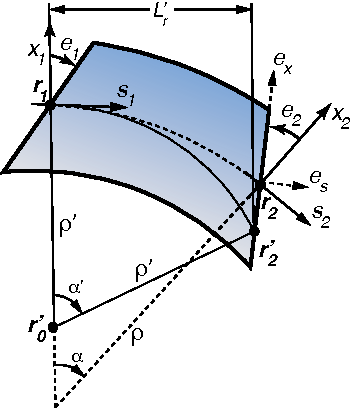
\includegraphics{bend-vary1.pdf}
    \caption{
With \vn{fiducial_pt} set to \vn{entrance_end}, $\bfr_1$ is the fiducial point at the entrance
end.  By construction, the entrance point $\bfr_1$ and the
slope of the reference curve at $\bfr_1$ is invariant with the reference curve before (dashed line)
and after (solid line) being tangent to $\bfs_1$ where $\bfs_1$ being the perpendicular to $\bfx_1$.
    }
    \label{f:bend.fid1}
  \end{subfigure}
  \hfill
  \begin{subfigure}[b]{0.4\textwidth}
    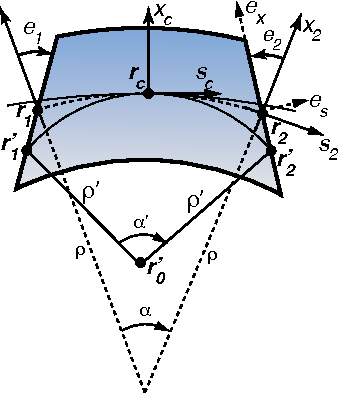
\includegraphics{bend-vary2.pdf}
    \caption{
With \vn{fiducial_pt} set to \vn{center}, $\bfr_c$ is the fiducial point at the center. By
construction, the reference curve always goes through $\bfr_c$ and the tangent of the reference
curve at $\bfr_c$ is invariant.}
    \label{f:bend.fid2}
  \end{subfigure}
  \hfill
  \caption{
Geometry with \vn{fiducial_pt} set to (a) \vn{entrance_end} and (b) \vn{center}. In both cases,
$\bfr_1$ and $\bfr_2$ are the entrance and exit reference points before and $\bfr'_1$ and $\bfr_2$
are the entrance and exit points after variation of one of \vn{rho}, \vn{g}, \vn{b_field}, or
\vn{angle}.  Similarly, $\rho$ and $\alpha$ are the bending radius and bending angle before
variation while $\rho'$ and $\alpha'$ are the bending radius afterwards.  Finally, $e_1$ $e_2$
are the face angles and rectangular length before variation, and $L'_r$ and $\bfr'_0$ are the
rectangular length and center of curvature after variation.
  }
  \label{f:bend.fid}
\end{figure}

\fig{f:bend.fid} shows the situation when the \vn{fiducial_pt} is set to either \vn{entrance_end} or
\vn{center} (the situation for the \vn{exit_end} setting is analogous to the \vn{entrance_end}
setting and so is not discussed). For any one of the \vn{fiducial_pt} settings discussed there are
essentially two cases. One case is direct variation of the bend field via variation of \vn{rho},
\vn{g}, or \vn{b_field}. This is called ``\vn{g}-variation''. The other type of variation is
variation of \vn{angle}. This is called ``angle-variation''. The discussion below shows how, with
\vn{g}-variation, \vn{l}, \vn{e1}, and \vn{e2} are calculated. With \vn{angle}-variation, \vn{l},
\vn{g}, \vn{e1}, and \vn{e2} need to be calculated. Once \vn{l} and \vn{g} are know, the other
parameters \vn{l_chord}, \vn{l_rectangle}, \vn{l_sagitta} (and \vn{angle} for the \vn{g}-variation
case) can be readily computed.

The \vn{entrance_end} analysis is as follows (\fig{f:bend.fid1}). The entrance end coordinates
around the point $\bfr_1$ are held fixed and as as a result $\bfr'_1 = \bfr_1$ and \vn{e1} does not
vary as well. $\bfr_2$ is the exit point before variation and $\bfr_3$ is the exit point after. The
position of $\bfr_3$ is calculated by first calculating the position of $\bfr_1$ in a coordinate
system centered at $\bfr_2$ and with axes parallel to the $(\bfs_1, \bfx_1)$ axes of the coordinate
system at $\bfr_1$
\begin{equation}
  \bar\bfr_1 = \left( -l_{\text{rectangle}}, \rho \, (1 - \cos\alpha) \right)
\end{equation}
Where the bar denotes that the coordinates are in the $(\bfs_1, \bfx_1)$ system.
The coordinates of $\bfr_1$ in the $(\bfe_s, \bfe_x)$ coordinate system
with origin at $\bfr_2$ and with $\bfe_x$ along the bend edge and $\bfe_s$ perpendicular to $\bfe_x$
is a rotation $\bfR(\theta)$ 
\begin{equation}
  \bfr_1 = \bfR(\alpha - e_2) \, \bar\bfr_1
\end{equation}
The angle $\theta_1$ of the vector $\bfs_1$, which is the invariant tangent of the reference curve
at the point $\bfr_1$, in the $(\bfe_s, \bfe_x)$ coordinate system (which is used from here on) is
\begin{equation}
  \theta_1 = \alpha - e_1
\end{equation}
The center of curvature after variation $\bfr'_0$ is 
\begin{equation}
  \bfr'_0 = \bfr_1 + \rho' \, \left( \sin\theta_1, -\cos\theta_1 \right)
\end{equation}
The reference trajectory after variation $\bfr'$ is a circular arc subject to the condition
\begin{equation}
  \left| \bfr' - \bfr'_0 \right| = \rho'^2
  \label{rr0r}
\end{equation}
With \vn{g}-variation, the value of $\rho'$ is set (perhaps indirectly) by the User. To find the
point $\bfr'_2$, it is noted that in the $(e_s, e_x)$ coordinate system,  the $s$
coordinate of $\bfr'_2$, $r'_{2s}$ is zero.
so using this in\Eq{rr0r} and throwing away the unphysical root gives for the $x$ coordinate
\begin{equation}
  r'_{2x} = r_{1x} + \frac{2 \, c}{-b - \sqrt{b^2-4 \, a \, c}}
\end{equation}
where
\begin{align}
  a &= g' \CRNO
  b &= 2 \, \cos\theta_1 \\
  c &= g' \, r_{1s}^2 + 2 \, r_{1s} \, \sin\theta_1 \nonumber
\end{align}
where $g' = 1 / \rho'$.
The rectangular length after variation $L'_r$ is then
\begin{equation}
  L'_r = L_r + r'_{2x} * \sin\theta_1
\end{equation}
where $L_r$ is the rectangular length before variation.
Finally, the length $L'$ after variation is
\begin{equation}
  L' = \text{asinc} \left( g' \, L'_r \right) \, L'_r
\end{equation}
where $\text{asinc}$ is the function
\begin{equation}
  \text{asinc}(\theta) = \frac{\sin^{-1}(\theta)}{\theta}
\end{equation}

For \vn{fiducial_pt} set to \vn{entrance_end} and with \vn{angle}-variation, $\alpha'$ is know and
$g'$ can be computed via
\begin{equation}
  g' = \frac{\sin(\alpha' - \theta_1) + \sin(\theta_1)}{r_{1s}}
  \label{gatt}
\end{equation}
With this, all other parameters can be created. In both \vn{angle}-variation and \vn{g}-variation the new
face angle $e'_2$ is given by
\begin{equation}
  e'_2 = e_2 + \alpha' - \alpha
\end{equation}

For \vn{fiducial_pt} set to \vn{center}, The center point $\bfr_c$ (see \fig{f:bend.fid2}) is held
constant.  Here the \vn{g}-variation analysis is similar to the \vn{g}-variation analysis with
\vn{fiducial_pt} set to \vn{entrance_end} (or \vn{exit_end} except in this case the reference orbit
to the right and left of $bfr_c$ are analyzed separately and the two lengths for each piece are
added together. For \vn{angle}-variation, the only situation where it is possible to keep $\bfr_c$
fixed while varying the angle is when \vn{e1} and \vn{e2} are equal. In this instance, the
calculation is again similar to the \vn{angle}-variation analysis with the \vn{fiducial_pt} set to
either end. If \vn{e1} and \vn{e2} are not equal, a calculation is done that gives the desired angle
but the center point will shift.

%---------------------------------------------------------------------------------
%---------------------------------------------------------------------------------
\section{Converter Tracking}
\label{s:converter.track}
\index{converter} 

Tracking through a \vn{converter} element involves generating five random numbers
  \footnote{
Since the outgoing particle starts at the exit surface of the converter only five numbers
are needed to generate the 6-dimensional particle phase space position.
  }
and then using these numbers with the outgoing particle distribution to generate the position and
orientation of the outgoing particle. The outgoing particle distribution is pre-computed by a
program \vn{converter_element_modeling} and the distribution parameters are included in the
converter element description in the \bmad lattice file (\sref{s:converter}). The accuracy of the
converter modeling will depend in part upon the granularity of the the probability tables generated
by the \vn{converter_element_modeling} program and on other approximations made during
tracking. Generally, inaccuracies in the 1\% to 10\% range are to be expected.

In a tracking simulation, a single outgoing particle is generated for each incoming particle. Since,
in a real machine, the number of outgoing particles will not be equal to the number of incoming
particles, each outgoing particle is assigned a weight such that the weighted distribution of
outgoing particles is correct. This weight will be the same for all outgoing particles. The weight
will depend upon whether the momentum or angular range of the outgoing particles is restricted using
the element parameters (\sref{s:converter}):
\begin{example}
  pc_out_min    ! Minimum momentum of generated outgoing particles (eV).
  pc_out_max    ! Maximum momentum of generated outgoing particles (eV).
  angle_out_max ! Maximum angle to the surface perpendicular (rad).
\end{example}

%-------------------------------------------------------------------------

\begin{figure}[tb]
  \centering
  \includegraphics[width=5in]{converter.pdf}
  \caption[Converter geometry.]
  {
An incoming particle strikes the bottom of the converter. At some point within the interior, a new
particle is generated and this new particle exits the top surface. To calculate the position and
orientation of the outgoing particle, a coordinate system is established where the origin point
$\wt\calO$ is the point that the incoming particle would strike the top surface if it went straight
through and the $(x,y)$ axes are randomly rotated with respect to the $(x_b,y_b)$ body coordinate axes.
By construction, the position of the outgoing particle will be along the $x$-axis.
  }
  \label{f:converter}.
\end{figure}

%-------------------------------------------------------------------------

The geometry of the converter is shown in \fig{f:converter}. On the top surface, where the outgoing
particle emerges, $(x_b,y_b)$ are the axes for the element body coordinate system (\sref{s:coords.3}).
To generate the position and orientation of the outgoing particle, another coordinate system is used
with axes labeled by $(x,y)$. Each outgoing particle will be assigned its own $(x,y)$
axes. The origin $\wt\calO$ of this coordinate system is constructed by placing $\wt\calO$ at the
point where the incoming particle under consideration would strike the top surface if the incoming
particle would pass straight through the converter. The angular orientation of the $(x,y)$ axes
with respect to the $(x,y)$ axes is chosen using a random number with a uniform probability
distribution in the interval $[0, \pi]$. By construction, the outgoing particle, at the surface of
the converter will be generated at a point a distance $r$ along the $x$-axis.

The particle distribution is calculated at a number of converter thickness $t_i$, $i = 1 \ldots
N_t$. It is an error if the actual converter thickness is outside the range of these
thicknesses. [The exception is if only one distribution for a given thickness is present, this
distribution is used to generate the outgoing particle coordinates independent of the converter
thickness.]  The particle distribution is also calculated within a certain incoming particle
momentum range. It is also an error if an incoming particle has a momentum outside of this range.

The first step is to choose the value of the outgoing particle's momentum $p_\txt{out}$. For each
thickness $t_i$, the pre-computed particle distribution parameters includes a two-dimensional table
of $P(p_\txt{out}, r)$ --- the probability density of creating an outgoing particle versus
$p_\txt{out}$ and $r$. $P(p_\txt{out},r)$ is normalized so that the integrated probability is equal
to the average number of outgoing particles created for each incoming particle $N_\txt{out}/N_{in}$
\begin{equation}
  \frac{N_\txt{out}}{N_{in}} = \int \int dp_\txt{out} \, dr \, P(p_\txt{out}, r)
  \label{nnprp}
\end{equation}
The integrals are done using linear interpolation between grid points.  From a $P(p_\txt{out},r)$
probability table, a ``normalized'' probability $P_\txt{n}(p_\txt{out},r)$ table is computed where
$P_\txt{n}$ is the probability of generating a particle at given $p_\txt{out}$ and $r$ with an
angular range restricted by \vn{angle_out_max}. If \vn{angle_out_max} is not set, $P_\txt{n}$ will
be equal to $P$.  This calculation is part of a ``setup'' computation done before tracking which, to
save time, is only done if one of the three element parameters, \vn{pc_out_min}, \vn{pc_out_max}, or
\vn{angle_out_max}, changes. Additionally, the setup includes creating a table of $I(p_\txt{out})$
which is the integrated probability for generating a particle with momentum less than $p_\txt{out}$
\begin{equation}
  I_p(p_\txt{out}) = \frac{\dstyle \int_{p_\txt{min}}^{p_\txt{out}} d\pw_\txt{out} 
  \int dr \, P_\txt{n}(\pw_\txt{out}, r)}
  {\dstyle \int_{p_\txt{min}}^{p_\txt{max}} d\pw_\txt{out} \int dr \, P_{n}(\pw_\txt{out}, r)}
\end{equation}
where $p_\txt{min}$ is the minimum momentum in the $P(p_\txt{out}, r)$ table or the value of
\vn{pc_out_min} which ever is greatest and $p_\txt{max}$ is the maximum momentum in the
$P(p_\txt{out}, r)$ table or the value of \vn{pc_out_max} which ever is smallest. $I(p_\txt{out})$
is normalized such that $I(p_\txt{max}) = 1$. A value for $p_\txt{out}$ is generated by solving
numerically for $p_\txt{out}$ the equation
\begin{equation}
  I_p(p_\txt{out}) = R_1
\end{equation}
where $R_1$ is a random number with uniform distribution in the interval $[0,1]$.  This
calculation is done for the two $t_i$ thicknesses that straddle the actual thickness. The value of
$p_\txt{out}$ assigned to the outgoing particle is obtained via linear interpolation between the two
computed values. Note that for both thicknesses the same random number needs to be used.

The next step is to choose a value for $r$. This is done by solving the equation
\begin{equation}
  I_r(r) = R_2
\end{equation}
where $R_2$ is another random number with uniform distribution in the interval $[0,1]$ and $I_r$ is 
\begin{equation}
  I_r(r) = \frac{\dstyle \int_0^r d\rw \, P_\txt{n}(p_\txt{out}, \rw)}
  {\dstyle \int_0^{r_\txt{max}} d\rw \, P_{n}(p_\txt{out}, \rw)}
\end{equation}
with $p_\txt{out}$ being the momentum chosen for the particle and $r_\txt{max}$ being the maximum
radius the probability table goes out to\footnote
  {
The range $[0,r_\txt{max}]$ encompasses nearly all of the outgoing particles. In principle, the
integral could be extended by extrapolating the values in the table but this could potentially lead
to inaccuracies in determining the outgoing orientation. Generally the inaccuracy in truncating the
distribution at $r_\txt{max}$ should be small.
  }. 
Like $p_\txt{out}$, this calculation is done for the two
$t_i$ thicknesses that straddle the actual thickness. The value of $r$ assigned to the outgoing
particle is obtained via linear interpolation between the two computed values. Note that for both
thicknesses the same random number needs to be used.

Once $p_\txt{out}$ and $r$ have been chosen, the next steps are to choose values for the angular
orientation of the outgoing particle. The angular orientation is characterized by the distribution
parameters using the derivatives $x' = dx/ds$ and $y' = dy/ds$ in the form of a skewed Lorentzian
probability distribution $P_d$
\begin{equation}
  P_d\left( x', y' ; p_\txt{out}, r \right) =
  A_d \, \frac{1 + \beta \, x'}{1 + \alpha_x^2 \, \left( x' - c_x \right)^2 +
  \alpha_y^2 \, \left( y' \right)^2}
  \label{pxsxs}
\end{equation}
where the parameters $A_d$, $\beta$, $c_x$, $\alpha_x$, and $\alpha_y$ all depend upon $p_\txt{out}$
and $r$. Notice that by construction, with the outgoing particle generated on the $x$-axis, the
distribution is symmetric about $y'$-axis. The pre-computed distribution characterizes each of these
parameters by a set of one or more fits which are functions of $p_\txt{out}$ and $r$. There are also
four functions of $p_\txt{out}$ and $r$ that give the range over which \Eq{pxsxs} is valid
$x'_\txt{min}$, $x'_\txt{max}$, $y'_\txt{min}$, and $y'_\txt{max}$. By symmetry, $y'_\txt{min} =
-y'_\txt{max}$. Also $A_d$ can be computed from knowledge of $\beta$, $c_x$, $\alpha_x$, and
$\alpha_y$ using the normalization condition that at any given $p_\txt{out}$ and $r$
\begin{equation}
  1 = \int_{x'_\txt{min}}^{x'_\txt{max}} dx' 
  \int_{-y'_\txt{max}}^{y'_\txt{max}} dy' \, P_d \left( x', y' \right)
\end{equation}
Thus there are only seven independent parameters that need to be fitted. The fit functions for all
seven have the same form. The fit is divided into two regions. For $p_\txt{out}$ lower than some
cutoff, a parameter is fit using a set of one-dimensional functions $\Gamma_i(r)$ at discrete momentum $p_i$,
$i = 1, \ldots, N_\beta$ with
\begin{equation}
  \Gamma_i(r) = \sum_{n=1}^M c_{n,i} \, r^n
  \label{gcr}
\end{equation}
The polynomial cutoff $M$ is 4 for $c_x$ and $\beta$ and is 3 for the other five.  To evaluate a
parameter at momenta lower than $p_{N_\beta}$, the $\Gamma_i$ are used with linear interpolation in
$p$ between functions of different $p_i$. At higher energies, the parameter variation is smoother so
a two dimensional fit $Xi$ is used
\begin{equation}
  \Xi(p_\txt{out},r) = e^{-(k_p \, p_\txt{out} + k_r \, r)} \,
  \left( \sum_{n=0}^3 k_{n} \, r^n \right) \, 
  \left( 1 + \sum_{n=1}^3 w_{n} \, p_\txt{out}^n \right) + C
  \label{xkpkr}
\end{equation}
The $C$ parameter is only nonzero for $x'_\txt{min}$. 

Once $A_d$, $\beta$, $c_x$, $\alpha_x$, and $\alpha_y$ have been calculated for a given $p_\txt{out}$ and
$r$, The calculation of $x'$ starts with integrating $P_d$ in \Eq{pxsxs} over $y'$
\begin{align} 
  I_{xd} (x') &\equiv \int_{-y'_\txt{lim}}^{y'_\txt{lim}} dy' \, P_d(x', y')
  \label{ixdyp} \\
  &= 2 \, A_d \, \frac{1 + \beta \, x'}{\alpha_y \, \sqrt{1 + \alpha_x^2 \, (x' - c_x)^2 }} \,
  \tan^{-1} \left( \frac{\alpha_y \, y'_\txt{lim}}{\sqrt{1 + \alpha_x^2 \, (x' - c_x)^2}} \right)
  \nonumber
\end{align}
where $y'_\txt{lim}$ is either the lesser of $y'_\txt{max}$ and $\tan^{-1}(\text{angle_out_max})$.
A spline fit is used to integrate $I_{xd}$ and this is used to choose a value for $x'$. Once $x'$
is known, The integral of $P_d(x', y')$ over $y'$ is used to choose a value for $y'$.

Except for the placement of $\wt\calO$, the above algorithm for calculating the position and
orientation of the outgoing particle will be independent of the angular orientation of the incoming
particle. This is valid for incoming particles that are traveling perpendicular to the converter
surface. To the extent that the incoming particles are not perpendicular to the converter, this will
introduce inaccuracies. Typically, however, the incoming particles will be fairly close to being
perpendicular. Considering this, and considering the approximations used to calculate the
distribution parameters, the neglect of incoming particle orientation effects is usually justified.

%---------------------------------------------------------------------------------
%---------------------------------------------------------------------------------
\section{Drift Tracking}
\label{s:drift.std}
\index{drift} 

\bmad uses the exact map for a drift
This gives the map
\begin{align}
  x_2    &= x_1 + \frac{L \, p_{x1}}{(1 + p_{z1}) \, p_l} \CRNO
  p_{x2} &= p_{x1}  \CRNO
  y_2    &= y_1 + \frac{L \, p_{y1}}{(1 + p_{z1}) \, p_l} \CRNO
  p_{y2} &= p_{y1}  \\
  z_2    &= z_1 + \left( \frac{\beta}{\beta_\REF} - \frac{1}{p_l} \right) \, L \CRNO
  p_{z2} &= p_{z1} \nonumber
\end{align}
where $\beta$ is the normalized particle velocity, $\beta_\REF$ is 
the reference particle's normalized velocity, and $p_l$ is the
longitudinal momentum
\begin{equation}
  p_l = \sqrt{1 - \frac{p_x^2 + p_y^2}{(1 + p_z)^2}}
\end{equation}

%---------------------------------------------------------------------------------
%---------------------------------------------------------------------------------
\section{ElSeparator Tracking}
\label{s:elsep.std}
\index{elseparator}

\begin{figure}[tb]
  \centering
  \includegraphics[width=5in]{elseparator.pdf}
  \caption[ElSeparator electric field.]
  {
Elseparator Electric field. The fringe field lines break the
translational invariance in $x$.
  }
  \label{f:elsep}.
\end{figure}

[Thanks to \'Etienne Forest for the derivation of the elseparator equation of motion.]

The Hamiltonian for an electric separator is 
\begin{equation}
  H = -p_s 
  = - \left\{ \left( \frac{1}{\beta_0} + \delta + k_E \, x \right)^2 - 
  \wt m^2 - p_x^2 - p_y^2 \right\}^{1/2}
  \label{hp1b}
\end{equation}
Here the canonical coordinates $(-c \, t, \delta$ are being used, $\wt m$ is defined in \Eq{mmccp},
and $p_s = -H$ is just the longitudinal momentum.  In the above equation, $k_E$ is the normalized
field
\begin{equation}
  k_E = \frac{q \, E}{P_0 \, c}
\end{equation}
The field is taken to be pointing along the $x$-axis with positive $k_E$ accelerating a particle in
the positive $x$ direction. To solve the equations of motion, a ``hard edge'' model is used where
$k_E$ is constant inside the separator and the field ends abruptly at the separator edges.

\index{solenoid}
Since, as shown in \fig{f:elsep}, the fringe fields break the translational invariance in $x$, it is
important here that the $x = 0$ plane be centered within the separator plates. With this, the
canonical momentum $\delta$ just outside the separator assumes its free space form of $\delta = (E -
E_0) / E_0)$. This is analogous to the case of a \vn{solenoid} where, to ensure that the canonical
transverse momenta assume their free space form just outside the solenoid, the $\Bf z$-axis must be
along the centerline of the solenoid.

The solution of the equations of motion is:
\begin{align}
  x   &= (x_0 - x_c) \, \cosh \left( \frac{k_E \, L}{p_s} \right) + 
         \frac{p_{x0}}{k_E} \, \sinh \left( \frac{k_E \, L}{p_s} \right) + x_c \CRNO
  p_x &= k_E \, (x_0 - x_c) \, \sinh \left( \frac{k_E \, L}{p_s} \right) + 
         {p_{x0}} \, \cosh \left( \frac{k_E \, L}{p_s} \right) \CRNO
  y   &= y_0 + L \, \frac{p_{y0}}{p_s} \label{xxlp} \\
  p_y &= p_{y0} \CRNO
  c \, \delta t &=  \int_0^L -\frac{\partial H}{\partial \delta}
      = (x_0 - x_c) \, \sinh \left( \frac{k_E \, L}{p_s} \right) +
        \frac{p_{x0}}{k_E} \, \left[ \cosh \left( \frac{k_E \, L}{p_s} \right) - 1 \right]
        \nonumber
\end{align}
where the critical position $x_c$ is
\begin{equation} 
  x_c = -\frac{\wt E}{k_E}
\end{equation}
and 
\begin{equation}
  \wt E \equiv \frac{1}{\beta_0} + \delta = \frac{E}{P_0 \, c}
\end{equation}
 
\Eqs{xxlp} predict that for $x < x_c$ and $p_{x0} = 0$ a particle will, unphysically, accelerate in
the negative $x$ direction. In actuality, a particle in this instance will be reflected backwards by
the longitudinal component of the edge field. Specifically, the argument of the square root in
\Eq{hp1b} must be non-negative and a particle will only make it through the separator if
\begin{equation}
  x_0 > \frac{1}{k_E} \, \left( \sqrt{\wt m^2 + p_{x0}^2 + p_{y0}^2} - \wt E \right)
\end{equation}

%---------------------------------------------------------------------------------
%---------------------------------------------------------------------------------
\section{Foil Tracking}
\label{s:foil.std}
\index{foil}

A particle going through a \vn{foil} element is scattered both in angle and in energy, and the
charge of the particle may be affected. The following two subsections give the formulas used for
scattering and energy loss. Currently, the final charge is a fixed number but that may change in the
future.

%---------------------------------------------------------------------------------
\subsection{Scattering in a Foil}
\label{s:foil.scatter}

For the angle scattering, the user can select between one of two algorithms, both
of which are given in the paper by Peralta and Louro\cite{b:peralta} (also see Lynch and Dahl\cite{b:lynch})
Both methods vary the phase space $p_x$ and $p_y$ coordinates using:
\begin{equation}
  (dp_x, dp_y) = \frac{p \, \sigma}{P_0} \, (r_1, r_2)
  \label{dpr1s}
\end{equation}
where $p$ is the
particle momentum, $P_0$ is the reference momentum, $r_1$ and $r_2$ are Gaussian random numbers with
unit sigma and zero mean, and $\sigma$ is the sigma of the angular scattering distribution. The
factor of $p/P_0$ is due to a translation between change in angle and change in phase space momenta
(see \Eq{xpa1p}). 

The \vn{Highland} algorithm uses Eq.~(32) of Peralta and Louro\cite{b:peralta} to calculate the
scattering sigma:
\begin{equation}
  \sigma = \frac{(13.6 \cdot 10^6~eV) \, z}{p \, c \, \beta} \sqrt{\frac{X}{X_0}} \, \left[
  1 + 0.038 \, \ln \left( \frac{X \, z^2}{X_0 \, \beta^2} \right) \right]
  \label{sszpb}
\end{equation}
where $X_0$ is the material radiation ``length'' in kg/m$^2$, $z$ is the particle charge, $\beta$ is the particle
relativistic beta, $c$ is the speed of light, and $X$ is the foil area density in kg/m$^2$ equal
to $\rho \, t$ where $\rho$ is the material density and $t$ is the foil thickness.

The \vn{Lynch_Dahl} algorithm uses Eq.~(33) of Peralta and Louro:
\begin{equation}
  \sigma^2 = \frac{\chi_c^2}{1 + F^2} \left[ \frac{1 + \nu}{\nu} \ln (1 + \nu) - 1 \right]
  \label{sc1f}
\end{equation}
where
\begin{align}
  \nu &= \frac{0.5 \, \Omega}{(1 - F)} \CRNO
  \Omega &= \frac{\chi_c^2}{1.167 \, \chi_\alpha^2} \CRNO
  \chi_c^2 &= \left( 1.57 \cdot 10^{10} \, \frac{eV^2 \, m^2}{kg} \right) \, 
    \frac{Z (Z+1) X}{A} \left[ \frac{z}{p \, \beta} \right]^2 
  \label{no1f} \\
  \chi_\alpha &= (2.007 \cdot 10^7 \, eV^2) \, \frac{Z^{2/3}}{(p \, c)^2} 
            \left[1 + 3.34 \,  \left( \frac{Z \, z \, \alpha}{\beta} \right)^2 \right] \nonumber
\end{align}
and the $A$ is the atomic weight, $p$ is the particle momentum, $\alpha$ is the fine structure
constant, and $F$ is a fit parameter representing the percent of the central angular distribution
that is used.  $F$ is a settable parameter with a default value of 0.98.

For compound materials, the value of $X/X_0$ in \Eq{sszpb} is computed from
\begin{equation}
  \frac{X}{X_0} = \sum_{i = 1}^N \frac{X_i}{X_{0i}}
\end{equation}
where the summation is over all constituents in the material.

Also for compound materials, $\chi_c^2$ in \Eqs{sc1f} and \eq{no1f} is replaced by the sum of the
constituent $\chi_{ci}^2$, and $\chi_\alpha$ is computed from Lynch and Dahl Eq.~(11)
\begin{equation}
  \ln ( \chi_\alpha ) = \left. \sum_{i=1}^N \frac{Z_i (Z_i + 1) X_i}{A_i} \ln(\chi_{\alpha i}) \middle/
  \sum_{i=1}^N \frac{Z_i (Z_i + 1) X_i}{A_i} \right.
\end{equation}

The actual scattering distribution has $1/\theta^4$ tails ($\theta$ is the scattering angle) due to
single event large angle scattering (Rutherford scattering). By assuming a Gaussian distribution,
these tails are not present in a simulation. It is also important to note that with both the
\vn{Highland} and \vn{Lynch_Dahl} algorithms, simulating the passage of particles through a single
foil versus two foils with half the thickness as the single foil will not give exactly the same
results. This is just a reflection that both algorithms are trying to model an inherently non-Gaussian
process.

%---------------------------------------------------------------------------------
\subsection{Energy Loss in a Foil}
\label{s:foil.eloss}

The particle energy loss per unit length $dE/dx$ through a foil is calculated using the \vn{Bethe-Bloch} formula
\begin{equation}
  - \left\langle\frac{dE}{dx}\right\rangle = 
  \frac{4 \pi}{m_e c^2} \cdot \frac{nz^2}{\beta^2} \cdot \left(\frac{e^2}{4\pi\varepsilon_0}\right)^2 \cdot 
  \left[\ln \left(\frac{2m_e c^2 \beta^2}{I \cdot (1-\beta^2)}\right) - \beta^2\right]
  \label{ex4pmc}
\end{equation}
where $n$ is the material electron density, $I$ is the mean excitation energy, $z$ is the particle
charge, $c$ is the speed of light, $\epsilon_0$ is the vacuum permittivity, $\beta = {v}/{c}$, is
the normalized velocity, and $e$ and $m_e$ the electron charge and rest mass respectively.

Note that to keep the direction of travel of the particle constant when energy is lost, this implies
that $p_x/(1+p_z)$ and $p_y/(1+p_z)$ are to be held constant (\Eq{xpa1p}).

%---------------------------------------------------------------------------------
%---------------------------------------------------------------------------------
\section{Kicker, Hkicker, and Vkicker Tracking}
\label{s:kicker.std}
\index{kicker}
\index{hkicker}
\index{vkicker}
\index{elseparator}

The Hamiltonian for a horizontally deflecting kicker or separator is
\begin{equation}
  H = \frac{p_x^2 + p_y^2}{2 (1 + p_z)} - k_0 \, x 
\end{equation}
This gives the map
\begin{alignat}{2}
  x_2 &= x_1 + \frac{1}{1 + p_{z1}} \, \left( L \, p_{x1} + \frac{1}{2} k_0 \, L^2 \right), &
    p_{x2} &= p_{x1} + k_0 \, L, \CRNO
  y_2 &= y_1 + \frac{L \, p_{y1}}{1 + p_{z1}}, &
    p_{y2} &= p_{y1},  \\
  z_2 &= z_1 - \frac{L}{2 (1 + p_{z1})^2} \, 
    \left( p_{x1}^2 + p_{y1}^2 + p_{x1} \, k_0 \, L + \frac{1}{3} k_0^2 \, L^2 \right), \quad &
  p_{z2} &= p_{z1} \nonumber
\end{alignat}
The generalization when the kick is not in the horizontal plane is easily derived.

%---------------------------------------------------------------------------------
%---------------------------------------------------------------------------------
\section{LCavity Tracking}
\label{s:lcavity.std}
\index{lcavity}

For tracking using something like \vn{runge_kutta}, with \vn{field_calc} set to \vn{bmad_standard},
the fields are modeled by the equations given in Sections~\sref{s:rf.fields} and \sref{s:rf.fringe}.

For \vn{bmad_standard} tracking, and with \vn{cavity_type} set to \vn{standing_wave}, the transverse
trajectory through an \vn{Lcavity} is modeled using equations developed by Rosenzweig and
Serafini\cite{b:rosenzweig} (R\&S) with
\begin{equation}
  b_0 = 1, \qquad \text{and} \qquad b_{-1} = 1 
\end{equation}
and all other $b_n$ set to zero.

The transport equations in R\&S were developed in the ultra-relativistic limit with $\beta = 1$.  To
extend these equations to lower energies, the transport through the cavity body (R\&S Eq.~(9)) has
been modified to give the correct phase-space area at non ultra-relativistic energies:
\begin{equation}
  \begin{pmatrix}
    x \\ 
    x'
  \end{pmatrix}_2 = \sqrt{\frac{\beta_1}{\beta_2}} \, 
  \begin{pmatrix}
    \cos(\alpha)  &
        \sqrt{\frac{8}{\eta(\Delta\phi)}} \, \frac{\, \gamma_1}{\gamma'} \, \cos(\Delta\phi) \, \sin(\alpha) \\
    -\sqrt{\frac{\eta(\Delta\phi)}{8}} \, \frac{\gamma'}{\gamma_2 \, \cos(\Delta\phi)} \, \sin(\alpha) &
        \frac{\gamma_1}{\gamma_2} \, \cos(\alpha)
  \end{pmatrix}
  \,
  \begin{pmatrix}
    x \\ 
    x'
  \end{pmatrix}_1
  \label{xxpc}
\end{equation}
The added factor of $\sqrt{\beta_1/\beta_2}$ gives the matrix the correct determinant of $\beta_1 \,
\gamma_1 / \beta_2 \, \gamma_2$. {\em While the added factor of $\sqrt{\beta_1/\beta_2}$ does
correct the phase space area, the above equation can only be considered as a rough approximation for
simulating particles when $\beta$ is significantly different from 1. Indeed, the only accurate way
to simulate such particles is by integrating through the actual field [Cf.~Runge Kutta tracking
(\sref{s:tkm})]}.

The change in $z$ going through a cavity is calculated by first calculating the particle
transit time $\Delta t$
\begin{align}
  c \, \Delta t &= \int_{s_1}^{s_2} \!\! ds \,\, \frac{1}{\beta(s)} 
    = \int_{s_1}^{s_2} \!\! ds \, \frac{E}{\sqrt{E^2 - (mc^2)^2}} \CRNO
  &= \frac{c \, P_2 - c \, P_1}{G} = \frac{E_2 + E_1}{P_2 + P_1} \, \frac{L}{c}
\end{align}
where $L$ is the accelerating length and it has been assumed that the accelerating gradient $G$ is
constant through the cavity and retarding due to the particle's finite transverse momentum is
ignored. In this equation $\beta = v / c$, $E$ is the energy, and $P$ is the momentum. The change in
$z$ is thus
\begin{equation}
  z_2 = \frac{\beta_2}{\beta_1} \, z_1 - 
  \frac{\beta_2 \, L}{c} \, 
  \left(
  \frac{E_2 + E_1}{P_2 + P_1} - 
  \frac{\Ebar_2 + \Ebar_1}{\Pbar_2 + \Pbar_1}
  \right)
\end{equation}
where $\Pbar$ and $\Ebar$ are the momentum and energy of the reference particle.

Note that the above transport equations are only symplectic on-axis There are second order terms in
the transverse coordinates that are missing. To obtain a proper symplectic matrix, the
\vn{symplectify} attribute of an \vn{lcavity} element (\sref{s:symp}) can be set to True.

%---------------------------------------------------------------------------------
%---------------------------------------------------------------------------------
\section{Octupole Tracking}
\label{s:octupole.std}
\index{octupole}

The Hamiltonian for an upright octupole is
\begin{equation}
  H = \frac{p_x^2 + p_y^2}{2 (1 + p_z)} + \frac{k_3}{24} (x^4 - 6 \, x^2 \, y^2 + y^4)
\end{equation}

An octupole is modeled using a kick-drift-kick model.

%---------------------------------------------------------------------------------
%---------------------------------------------------------------------------------
\section{Patch Tracking}
\label{s:patch.std}
\index{patch}

\begin{figure}[tb]
  \centering
  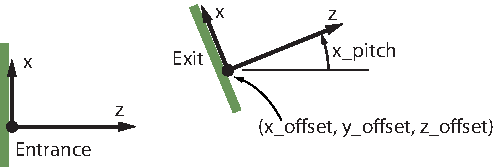
\includegraphics[width=5in]{patch.pdf}
  \caption[Standard patch transformation.]
{Standard tracking through a patch element. A particle's starting coordinate at the entrance end of
the patch has, by construction, coordinate $z$ = 0. The particle is drifted, as in a field free
region, between the entrance $z = 0$ plane and the exit $z = 0$ plane.}
  \label{f:patch.track}
\end{figure}

%---------------------------------------------------------------------------------

The transformation of the reference coordinates through a ``standard'' patch (a patch where custom
fields are not used) is given by \Eqs{vwlv} and \eq{wws}. At the entrance end of the patch, a
particle's position and momentum in the entrance coordinate system will be
\begin{alignat}{1}
  \bfr &= (x, y, 0) \CRNO
  \bfP &= (P_x, P_y, P_z) = 
    \left( p_x, p_y, \pm \sqrt{(1+p_z)^2 - p_x^2 - p_y^2} \right) \, P_{0\text{ent}}
\end{alignat}
where $p_x$, $p_y$ and $p_z$ are the phase space momenta, and $z$, which is coordinate $z$ and not
phase space $z$, is always zero by construction as shown in \fig{f:patch.track} [Also see
\fig{f:local.coords} and the discussion in \sref{s:phase.space}.] The sign of the longitudinal
momentum $P_z$ is determined by whether the particle is traveling in the positive $s$ or negative
$s$ direction (which will occur when an element is flipped longitudinally).

The transformation between entrance and exit coordinate systems is given by \Eqs{rwlr} and \eq{pps}
\begin{alignat}{1}
  \bfr &\rightarrow 
    \bfS^{-1} \, (\bfr - \bfL_\text{off}) \CRNO
  \bfP &\rightarrow \bfS^{-1} \, \bfP
\end{alignat}
where $\bfL_\text{off}$ is given by \Eq{swww}

After this transformation, the particle must be propagated by a longitudinal length
$-r_z$ to intersect the $r_z = 0$ plane of the exit face.
\begin{alignat}{1}
  \bfr &\rightarrow (r_x - r_z \, \frac{P_x}{P_z}, r_y - r_z \, \frac{P_y}{P_z}, 0) \CRNO
  \bfP &\rightarrow \bfP
\end{alignat}

The final $\bfr$ and $\bfP$ can now be used compute the particles
phase space coordinates, along with the time $t$ and the reference time
$t_\REF$ at the exit end.
\begin{alignat}{3}
  x &\rightarrow r_x \qquad &p_x &\rightarrow \frac{P_x}{P_{0\text{exi}}} \CRNO
  y &\rightarrow r_y \qquad &p_y &\rightarrow \frac{P_y}{P_{0\text{exi}}} \\
  z &\rightarrow z + r_z \, \frac{|\bfP|}{P_z} + L_0 \, \frac{\beta}{\beta_0} +
    \beta \, \text{t_offset} \qquad
    &p_z &\rightarrow \frac{(1+p_z) \, P_{0\text{ent}} - P_{0\text{exi}}}{P_{0\text{exi}}} \CRNO
  t &\rightarrow t - r_z \, \frac{|\bfP|}{P_z \, \beta} \qquad
  &t_\REF &\rightarrow t_\REF + \text{t_offset} + L_0 \, \frac{1}{\beta_0} \nonumber
\end{alignat}
where the exit reference momentum $P_{0\text{exi}}$ is related to the
entrance reference momentum $P_{0\text{ent}}$ through
\vn{e_tot_offset}.  In the above equation, $\beta$ is the particle
velocity, $\beta_0$ is the velocity of the reference particle, and
$L_0$ is the drift length of the reference particle
\begin{equation}
  L_0 = \frac{1}{S^{-1}_{33}} \, \left( 
  S^{-1}_{31} \, \text{x_offset} + S^{-1}_{32} \, \text{y_offset} + S^{-1}_{33} \, \text{z_offset}
  \right)
\end{equation}

%---------------------------------------------------------------------------------
%---------------------------------------------------------------------------------
\section{Quadrupole Tracking}
\label{s:quadrupole.std}
\index{quadrupole}

The \vn{bmad_standard} calculates the transfer map through an upright
quadrupole and then transforms that map to the laboratory frame.

The Hamiltonian for an upright quadrupole is
\begin{equation}
  H = \frac{p_x^2 + p_y^2}{2 (1 + p_z)} + \frac{k_1}{2} (x^2 - y^2)
\end{equation}
This is simply solved
\begin{align}
  x_2    &= c_x \, x_1 + s_x \, \frac{p_{x1}}{1 + p_{z1}} \CRNO
  p_{x2} &= \tau_x \, \om^2 \, \, (1 + p_{z1}) \, s_x \, x_1 + c_x \, p_{x1} \CRNO
  y_2    &= c_y \, y_1 + s_y \, \frac{p_{y1}}{1 + p_{z1}} \CRNO
  p_{y2} &= \tau_y \, \om^2 \, \, (1 + p_{z1}) \, s_y \, y_1 + c_y \, p_{y1} \\
  z_2    &= z_1 + m_{511} \, x_1^2 + m_{512} \, x_1 \, p_{x1} + m_{522} \, p_{x1}^2 + 
                   m_{533} \, y_1^2 + m_{534} \, y_1 \, p_{y1} + m_{544} \, p_{y1}^2 \CRNO
  p_{z2} &= p_{z1} \nonumber
\end{align}
where 
\begin{equation}
  \om \equiv \sqrt{\frac{|k_1|}{1 + p_{z1}}}
\end{equation}
and
\begin{alignat}{6}
         &\hspace*{3ex}  && k_1 > 0          &\hspace*{3ex}& k_1 < 0 & \qqquad
         &\hspace*{3ex}  && k_1 > 0          &\hspace*{3ex}& k_1 < 0 \CRNO
     c_x &=   && \cos  (\om \, L) && \cosh (\om \, L) & \qqquad
     c_y &=   && \cosh (\om \, L) && \cos  (\om \, L) \CRNO
     s_x &=   && \frac{\sin  (\om \, L)}{\om} && \frac{\sinh (\om \, L)}{\om} & \qqquad
     s_y &=   && \frac{\sinh (\om \, L)}{\om} && \frac{\sin  (\om \, L)}{\om} \\
  \tau_x &=   && {-}1             && {+}1             & \qqquad
  \tau_y &=   && {+}1             && {-}1             \nonumber
\end{alignat}
with this
\begin{alignat}{2}
  m_{511} &= \frac{\tau_x \,\, \om^2}{4} \, (L - c_x \, s_x) & \qqquad
  m_{533} &= \frac{\tau_y \,\, \om^2}{4} \, (L - c_y \, s_y) \CRNO
  m_{512} &= \frac{-\tau_x \,\, \om^2}{2 \, (1 + p_{z1})} \, s_x^2 & \qqquad
  m_{534} &= \frac{-\tau_y \,\, \om^2}{2 \, (1 + p_{z1})} \, s_y^2 \\
  m_{522} &= \frac{-1}{4 \, (1 + p_{z1})^2} \, (L + c_x \, s_x) & \qqquad
  m_{544} &= \frac{-1}{4 \, (1 + p_{z1})^2} \, (L + c_y \, s_y) \nonumber
\end{alignat}

%---------------------------------------------------------------------------------
%---------------------------------------------------------------------------------
\section{RFcavity Tracking}
\label{s:rfcavity.std}
\index{rfcavity}

For tracking using something like \vn{runge_kutta}, with \vn{field_calc} set to \vn{bmad_standard},
the fields are modeled by the equations given in Sections~\sref{s:rf.fields} and \sref{s:rf.fringe}.

With \vn{bmad_standard} tracking, a kick-drift-kick model is used. The kick is a
pure energy kick (see equations in \sref{s:rfcav}) and the phase of the RF is calculated under the
assumption that the waveform moves at a phase velocity equal to the velocity of the reference
particle.

With \vn{bmad_standard} tracking, the transverse forces due to the RF are ignored. This is generally
a reasonable approximation when the acceleration is small as is standard in rings. \vn{Lcavity}
elements should be used in place of \vn{rfcavity} elements when this is not so.

%---------------------------------------------------------------------------------
%---------------------------------------------------------------------------------
\section{Sad\_Mult Tracking}
\label{s:sad.mult.std}
\index{sad_mult}

The ``hard edge'' fringe field kick is taken from Forest\cite{b:forest} Eqs.~(13.29) and onward.
In the notation of \bmad, and taking into account both normal and skew terms, Eq.~(13.29)
is for the $m$\th order multipole (what Forest labels $n+1$)
\begin{equation}
  f_\pm = \mp \Re \frac{(b_m + i \, a_m) \, (x + i \, y)^{(m+1)}}{4 \, (m+2) \, (1 + p_z)}
    \left[ x \, p_x + y \, p_y + i\frac{m+3}{m+1}(x \, p_y - y \, p_x) \right]
\end{equation}

The ``soft edge'' dipole fringe for \vn{sad_mult} elements is a generalization of the soft edge
dipole fringe for a SAD bend element. For the entrance kick the equations are:
\begin{align}
  x_2 &= x_1 + \frac{\delta_1}{1 + \delta_1} \, \Delta x_{fx}, \qquad
  p_{x2} = p_{x1} + \frac{1}{1 + \delta_1} \, \left[ 
    \Delta x_{fy} \, v - \Delta x_{fay} \, v^3 \right] \CRNO
  y_2 &= y_1 - \frac{\delta_1}{1 + \delta_1} \, \Delta y_{fy}, \qquad
  p_{y2} = p_{y1} + \frac{1}{1 + \delta_1} \, \left[ 
    \Delta y_{fx} \, w - \Delta y_{fax} \, w^3 \right] \\
  z_2 &= z_1 + \frac{1}{(1 + \delta_1)^2} \, \left[ \, 
    \Delta x_{fx} \, p_{x1} - \Delta y_{fy} \, p_{y1} + 
    \frac{1}{2} \, (\Delta y_{fx} + \Delta x_{fy}) \, w^2 -
    \frac{1}{4} (\Delta y_{fax} + \Delta x_{fay}) \, w^4
    \right] \nonumber
\end{align}
where
\begin{alignat}{3}
  \Delta x_{fx}  &= \frac{K_0 \, F_B^2}{24 \, L}, & \qquad 
  \Delta y_{fx}  &= \frac{K_0^2 \, F_B}{6 \, L^2}, & \qquad 
  \Delta y_{fax} &= \frac{2 \, K_0^2}{3 \, F_B \, L^2}, \CRNO 
  \Delta y_{fy}  &= \frac{SK_0 \, F_B^2}{24 \, L}, & \qquad
  \Delta x_{fy}  &= \frac{SK_0^2 \, F_B}{6 \, L^2}, & \qquad
  \Delta x_{fay} &= \frac{2 \, SK_0^2}{3 \, F_B \, L^2}, \\
  v &= \cos\theta \, x_1 + \sin\theta \, y_1, & \qquad
  w &= -\sin\theta \, x_1 + \cos\theta \, y_1, & \qquad
  \tan\theta &= \frac{-SK_0}{K_0} \nonumber
\end{alignat}


%---------------------------------------------------------------------------------
%---------------------------------------------------------------------------------
\section{Sextupole Tracking}
\label{s:sextupole.std}
\index{sextupole}

The Hamiltonian for an upright sextupole is
\begin{equation}
  H = \frac{p_x^2 + p_y^2}{2 (1 + p_z)} + \frac{k_2}{6} (x^3 - 3 \, x \, y^2)
\end{equation}

Tracking through a sextupole uses a kick-drift-kick model.

%---------------------------------------------------------------------------------
%---------------------------------------------------------------------------------
\section{Sol\_Quad Tracking}
\label{s:sol.quad.std}
\index{sol_quad}

The Hamiltonian is
\begin{equation}
  H = \frac{(p_x + \frac{k_s }{2}\, y)^2}{2 (1 + p_z)} + 
  \frac{(p_y - \frac{k_s}{2} \, x)^2}{2 (1 + p_z)} + \frac{k_1}{2} (x^2 - y^2)
\end{equation}
Solving the equations of motion gives
\begin{align}
  x_2    &= m_{11} \, x_1 + m_{12} \, p_{x1} + m_{13} \, y_1 + m_{14} \, p_{y1} \CRNO
  p_{x2} &= m_{21} \, x_1 + m_{22} \, p_{x1} + m_{23} \, y_1 + m_{24} \, p_{y1} \CRNO
  y_2    &= m_{31} \, x_1 + m_{32} \, p_{x1} + m_{33} \, y_1 + m_{34} \, p_{y1} \CRNO
  p_{y2} &= m_{41} \, x_1 + m_{42} \, p_{x1} + m_{43} \, y_1 + m_{44} \, p_{y1} \\
  z_2    &= z_1 + \sum_{j = 1}^4 \sum_{k = j}^4 m_{5jk} \, r_j \, r_k  \CRNO
  p_{z2} &= p_{z1} \nonumber
\end{align}
where
\begin{alignat}{2}
  m_{11} &= \frac{1}{2 \, f} \, \left( f_{0+} \, c + f_{0-} \, c_h \right) & \qqquad
  m_{31} &= -m_{24} \CRNO
  m_{12} &= \frac{1}{2 \, f \, (1 + p_{z1})} \, 
            \left( \frac{f_{++}}{\om_+} \,  s + \frac{f_{--}}{\om_-} \, s_h \right) & \qqquad
  m_{32} &= -m_{14} \CRNO
  m_{13} &= \frac{\ks}{4 \, f} \, 
            \left( \frac{f_{+-}}{\om_+} \, s +\frac{f_{-+}}{\om_-} \, s_h \right) & \qqquad
  m_{33} &= \frac{1}{2 \, f} \, \left( f_{0-} \, c + f_{0+} \, c_h \right) \CRNO
  m_{14} &= \frac{\ks}{f \, (1 + p_{z1})} \, \left( -c + c_h \right) & \qqquad
  m_{34} &= \frac{1}{2 \, f \, (1 + p_{z1})} \, 
            \left( \frac{f_{+-}}{\om_+} \, s + \frac{f_{-+}}{\om_-} \, s_h \right) \CRNO
  m_{21} &= \frac{-(1 + p_{z1})}{8 \, f} \, 
            \left( \frac{\xi_{1+}}{\om_+} \, s + \frac{\xi_{2+}}{\om_-} s_h \right) & \qqquad
  m_{41} &= -m_{23} \\
  m_{22} &= m_{11} & \qqquad
  m_{42} &= -m_{13} \CRNO
  m_{23} &= \frac{\ks^3 \, (1 + p_{z1})}{4 \, f} \, \left( c - c_h \right) & \qqquad
  m_{43} &= \frac{-(1 + p_{z1})}{8 \, f} \, 
            \left( \frac{\xi_{1-}}{\om_+} \, s + \frac{\xi_{2-}}{\om_-} \, s_h \right) \CRNO
  m_{24} &= \frac{\ks}{4 \, f} \, 
            \left( \frac{f_{++}}{\om_+} \, s + \frac{f_{--}}{\om_-} \, s_h \right) & \qqquad
  m_{44} &= m_{33} \nonumber
\end{alignat}
and
\begin{alignat}{2}
  \kone        &= \frac{k_1}{1 + p_{z1}} & \qqquad 
  \ks          &= \frac{k_s}{1 + p_{z1}} \CRNO
  f            &= \sqrt{\ks^4 + 4 \, \kone^2} & \qqquad
  f_{\pm0}     &= f \pm \ks^2 \CRNO
  f_{0\pm}     &= f \pm 2 \, \kone & \qqquad
  f_{\pm\pm}   &= f \pm \ks^2 \pm 2 \, \kone \CRNO
  \om_+        &= \sqrt{\frac{f_{+0}}{2}} & \qqquad
  \om_-        &= \sqrt{\frac{f_{-0}}{2}} \\
  s            &= \sin (\om_+ \, L) & \qqquad
  s_h          &= \sinh (\om_- \, L) \CRNO
  c            &= \cos (\om_+ \, L) & \qqquad
  c_h          &= \cosh (\om_- \, L) \CRNO
  \xi_{1\pm} &= \ks^2 \, f_{+\mp} \pm 4 \, \kone \, f_{+\pm} & \qqquad
  \xi_{2\pm} &= \ks^2 \, f_{-\pm} \pm 4 \, \kone \, f_{-\mp} \nonumber
\end{alignat}

The $m_{5jk}$ terms are obtained via \Eq{zz121p}
\begin{align}
  m_{5jk} = - \frac{\tau_{jk}}{2 (1 + p_{z1})^2} \int \! ds \, 
  & \left[ 
    \left( m_{2j} + \frac{k_s}{2} \, m_{3j} \right) \, 
    \left( m_{2k} + \frac{k_s}{2} \, m_{3k} \right)   
  \right. + \\
  & \hspace*{15ex} \left.
    \left( m_{4j} - \frac{k_s}{2} \, m_{1j} \right) \, 
    \left( m_{4k} - \frac{k_s}{2} \, m_{1k} \right) 
  \right] \nonumber
\end{align}
where
\begin{equation}
  \tau_{jk} = 
  \begin{cases}
    1 & j = k \\
    2 & j \ne k 
  \end{cases}
\end{equation}
The needed integrals involve the product of two trigonometric or
hyperbolic functions. These integrals are trivial to do but the
explicit equations for $m_{5jk}$ are quite long and in the interests of
brevity are not reproduced here.

%---------------------------------------------------------------------------------

\begin{figure}[tb]
  \centering
  \includegraphics[width=5in]{solenoid.pdf}
  \caption[Solenoid with a hard edge.]
  {
Solenoid with a hard edge. The field is assumed to end abruptly at the edges of the solenoid. Here,
for purposes of illustration, the field lines at the ends are displaced from one another.
  }
  \label{f:solenoid}.
\end{figure}

%---------------------------------------------------------------------------------
\section{Solenoid Tracking}
\label{s:solenoid.std}
\index{solenoid}

The \vn{bmad_standard} solenoid tracking does not make the small angle approximation.
The transfer map for the solenoid is:
\begin{align}
  x_2    &= \frac{1 + c}{2} \, x_1 + \frac{s}{k_s} \, p_{x1} +
           \frac{s}{2} \, y_1 + \frac{1 - c}{k_s} \, p_{y1} \CRNO
  p_{x2} &= \frac{-k_s \, s}{4} \, x_1 + \frac{1 + c}{2} \, p_{x1} - 
           \frac{k_s \, (1 - c)}{4} \, y_1 + \frac{s}{2} \, p_{y1} \CRNO
  y_2    &= \frac{-s}{2} \, x_1 - \frac{1 - c}{k_s} \, p_{x1} +
           \frac{1 + c}{2} \, y_1 + \frac{s}{k_s} \, p_{y1} \\      
  p_{y2} &= \frac{k_s \, (1 - c)}{4} \, x_1 + \frac{-s}{2} \, p_{x1} -
            \frac{k_s \, s}{4} \, y_1 + \frac{1 + c}{2} \, p_{y1} \CRNO 
  z_2    &= z_1 + \frac{L \, (1 + p_{z1})^2}{2 \, p_r^3} \, 
                   \left[ \left( p_{x1} + \frac{k_s}{2} \, y_1 \right)^2 +
                          \left( p_{y1} - \frac{k_s}{2} \, x_1 \right)^2 \right] \CRNO
  p_{z2} &= p_{z1} \nonumber
\end{align}
where $k_s = B/P_0$ is the normalized field and
\begin{align}
  c &= \cos \left( k_s L / p_r \right) \CRNO
  s &= \sin \left( k_s L / p_r \right)
\end{align}
with
\begin{equation}
  p_r = \sqrt{(1 + p_z)^2 - (p_x + y_1 \, k_s/2)^2 - (p_y - x_1 \, k_s/2)^2}
\end{equation}

To be useful, the canonical momenta $p_x$ and $p_y$ in the above equations must be connected to the
canonical momenta used for other elements (drifts, quadrupoles, etc.) that may be placed to either
side of the solenoid. These side elements use zero $a_x$ and $a_y$ (cf. \Eq{pmc2pc}). The vector
potential used in the solenoid canonical momenta may be made zero at the edges of the solenoid if
the solenoid fringe field is assumed to end abruptly at the edges of the solenoid (as shown in
\fig{f:solenoid}), and the reference axis $\Bf z$-axis (at $x$ = $y$ = 0) is placed along the
centerline of the solenoid so that there is cylindrical symmetry around the $\Bf z$-axis.

%-----------------------------------------------------------------------------------------
\section{Sprint Spin Tracking}
\label{s:sprint.std}
\index{sprint spin tracking}

The \vn{sprint} spin tracking method is named after the \vn{SPRINT} program developed by Matthias
Vogt.  The \vn{sprint} algorithm Uses a first order spin map evaluated with respect to the zero
orbit to track through elements. This method is much faster than PTC integration, and its run-time
does not increase proportionally to element length. Currently, the supported lattice elements are
bends (including bends with $k_1 \neq 0$), quadrupoles, and solenoids \sref{s:spin.methods}.

Elements with fringe field contributions are split into three quaternions representing the entrance,
body, and exit of the element. Before propagation, the exit fringe quaternion is always equivalent
to the entrance fringe quaternion, with all field strengths multiplied by -1, and $e_1$ replaced
with $-e_2$. The exit quaternion is then propagated to the end of the element via Bmad mapping
tools. Appropriate quaternions are concatenated according to the values of \vn{spin_fringe_on} and
\vn{fringe_at}.

\begin{alignat}{8}
 & {d}    &&= g \, l              && {e}    &&= a \, g \, l\gamma   && s     &&= a \, k_s l       && {t}    &&= (1+a) k_s l         \CRNO
 & c_{d}  &&= \cos({d})    \qquad && s_{e2} &&= \sin(\frac{{e}}{2}) && c_{s} &&= \cos({s}) \qquad && c_{t}  &&= \cos({t})           \\
 & s_{d}  &&= \sin({d})           && c_{e2} &&= \cos(\frac{{e}}{2}) && s_{s} &&= \sin({s})        && s_{t2} &&= \sin(\frac{{t}}{2}) \CRNO
 & \chi   &&= 1+a\gamma           && \zeta  &&= \gamma - 1   \qquad && \psi  &&= \gamma^2 - 1     && c_{t2} &&= \cos(\frac{{t}}{2}) \nonumber
\end{alignat}

%-----------------------------------------------------------------------------------------
\subsection{SBend Body, $k_1 = 0$}

\begin{center}
\begin{tabular}{llll} \toprule
        & $q_0$    & $q_y$     & $q_z$ \\ \midrule
  $1$   & $c_{e2}$ & $-s_{e2}$ &       \\ \addlinespace[1ex]
  $x$   & $-\frac{1}{2} g \chi s_{d} s_{e2}$ & $-\frac{1}{2} g \chi \, s_{d} c_{e2}$ & \\ \addlinespace[1ex]
  $p_x$ & $\frac{1}{2} \chi \, (c_{d} - 1)  s_{e2}$ & $\frac{1}{2} \chi \, (c_{d} - 1) c_{e2}$ & \\ \addlinespace[1ex]
  $p_y$ &          &           & $\frac{1}{\gamma} \zeta \, s_{e2}$ \\ \addlinespace[1ex]
  $p_z$ & $\frac{1}{2 \gamma} \left(\gamma \, \chi \, s_{d} -a \, \psi \, {d} \right) s_{e2}$ & & \\
  \bottomrule
\end{tabular}
\end{center}

%-----------------------------------------------------------------------------------------
\subsection{Sbend Body, $k_1 \neq 0$}

\begin{equation}
\begin{aligned}
  &  k_x = k_1 + g^2 \\
  & \omega_x = \sqrt{|k_x|} \\
  & \omega_y = \sqrt{|k_1|}
\end{aligned}
\qquad\qquad\qquad
\begin{aligned}
  & \alpha = 2(a^2 g^2 \gamma^2 + k_1) \\ \nonumber
  & \beta = a g k_1 (\gamma \chi - \zeta) \\ \nonumber
  & \sigma = \omega_y (k_1 + a k_1 \gamma + a^2g^2 \zeta \gamma)\\ \nonumber
  & \xi = \omega_y (k_1 \chi + a^2 g^2 \zeta \gamma) \nonumber
\end{aligned}
\end{equation}

\begin{center}
\begin{tabular}{cccc}
  $k_x > 0$                  & $k_x < 0$              & $k_1 > 0$                   & $k_1 < 0$  \\
  $s_x = \sin{(l \omega_x)}$ & $ \sinh{(l \omega_x)}$ & $s_y = \sinh{(l \omega_y)}$ & $ \sin{(l \omega_y)}$ \\
  $c_x = \cos{(l \omega_x)}$ & $ \cosh{(l \omega_x)}$ & $c_y = \cosh{(l \omega_y)}$ & $ \cos{(l \omega_y)}$ \\
  $\tau_x = -1$              & $+1$                   & $\tau_y = +1$               & $-1$
\end{tabular}
\end{center}

\begin{center}
\begin{tabular}{lllll} \toprule
        & $q_0$    & $q_x$ & $q_y$     & $q_z$ \\ \midrule
  1     & $c_{e2}$ &       & $-s_{e2}$ &       \\ \addlinespace[1ex]
  $x$   & $\frac{-k_x \chi}{2 \omega_x} s_x s_{e2}$            &   &
    $\frac{-k_x \chi}{2 \omega_x} s_x c_{e2}$ & \\ \addlinespace[1ex]
  $p_x$ & $\frac{k_x \chi}{2\omega_x^2} \tau_x (1-c_x) s_{e2}$ &   &
    $\frac{k_x \chi}{2 \omega_x^2} \tau_x \left(1-c_x\right) c_{e2}$ & \\ \addlinespace[1ex]
  $y$   &          &
    {$\begin{aligned}
      \frac{-1}{\alpha} &\bigl[ \beta (1+ c_y) s_{e2} +{} \\[-1.5ex]
      & \hskip4.5em \tau_y \sigma s_y c_{e2} \bigr]
    \end{aligned}$} &  &
    {$\begin{aligned}
       \frac{1}{\alpha} &\bigl[ \beta (1-c_y) c_{e2} + {} \\[-1.5ex]
       & \hskip4.5em \tau_y \sigma s_y s_{e2} \bigr]
    \end{aligned}$} \\ \addlinespace[1ex]
  $p_y$ &          &
    {$\begin{aligned}
      \frac{1}{\omega_y \alpha} &\bigl[ \xi (1 - c_y) c_{e2} - {} \\[-1.5ex]
      & \hskip5em \beta s_y s_{e2} \bigr]
    \end{aligned}$} &   &
    {$\begin{aligned}
      \frac{1}{\omega_y \alpha} &\bigl[ \xi (1+c_y) s_{e2} - {} \\[-1.5ex]
      & \hskip5em \beta s_y c_{e2}\bigr]
    \end{aligned}$} \\ \addlinespace[1ex]
  $p_z$ & $\frac{g}{2}\left(\frac{\chi s_x}{\omega_x} - \frac{a l \psi}{\gamma}\right) s_{e2}$ &    &
    $\frac{g}{2}\left(\frac{\chi s_x}{\omega_x} - \frac{a l \psi}{\gamma}\right) c_{e2}$ & \\
  \bottomrule
  \end{tabular}
\end{center}

%-----------------------------------------------------------------------------------------
\subsection{Sbend Entrance Fringe}

To calculate the exit fringe, multiply all field strengths $g$ by
-1, and replace all entrance face angles $e_1$ with exit face angles $-e_2$. The negative exit face
angle is used due to Bmad convention.
\begin{center}
  \begin{tabular}{lllll} \toprule
      & $q_0$ & $q_x$                         & $q_y$                          & $q_z$ \\ \midrule
  1   & 1     &                               &                                & \\ \addlinespace[1ex]
  $x$ &       &                               & $\frac{1}{2} \chi g \tan(e_1)$ & \\ \addlinespace[1ex]
  $y$ &       & $\frac{1}{2}(1+a)g \sin(e_1)$ &                                & $-\frac{1}{2}(1+a)g \cos(e_1)$ \\
  \bottomrule
  \end{tabular}
\end{center}

%-----------------------------------------------------------------------------------------
\subsection{Quadrupole}

\begin{equation}
  \omega = \sqrt{|k_1|} \nonumber
\end{equation}

\begin{center}
\begin{tabular}{cccc}
  $k_1 > 0$ & $k_1 < 0$ & $k_1 > 0$ & $k_1 < 0$  \\
  $s_x = \frac{\sin{(l \omega)}}{\omega}$ & $ \frac{\sinh{(l \omega)}}{\omega}$ &$s_y = \frac{\sinh{(l \omega)}}{\omega}$ & $ \frac{\sin{(l \omega)}}{\omega}$ \\
  $c_x = \frac{1 - \cos{(l \omega)}}{\omega^2}$ & $ \frac{-1 + \cosh{(l \omega)}}{\omega^2}$ &$c_y = \frac{-1 + \cosh{(l \omega)}}{\omega^2}$ & $ \frac{1 - \cos{(l \omega)}}{\omega^2}$ \\
\end{tabular}
\end{center}
\everymath{}

\begin{center}
\begin{tabular}{llll} \toprule
        & $q_0$ & $q_x$ & $q_y$ \\ \midrule
  1     & 1     &       &       \\ \addlinespace[1ex]
  $x$   &       &       & $-\frac{1}{2} k_1 \chi s_x$ \\ \addlinespace[1ex]
  $p_x$ &       &       & $-\frac{1}{2} k_1 \chi c_x$ \\ \addlinespace[1ex]
  $y$   &       & $-\frac{1}{2} k_1 \chi s_y$ & \\ \addlinespace[1ex]
  $p_y$ &       & $-\frac{1}{2} k_1 \chi c_y$ & \\
\bottomrule
\end{tabular}
\end{center}

%-----------------------------------------------------------------------------------------
\subsection{Solenoid Element Body}

\begin{center}
\begin{tabular}{lllll} \toprule
  &  $q_0$ & $q_x$ & $q_y$ & $q_z$ \\ \midrule
  1 & $c_{t2}$ & & & $-s_{t2}$ \\ \addlinespace[1ex]
  $x$ & & $\frac{1}{4} k_s \zeta ((1 - c_{s}) c_{t2} - s_{s} s_{t2})$ & $\frac{1}{4} k_s \zeta ((-1 + c_{s}) s_{t2} - s_{s} c_{t2})$ & \\ \addlinespace[1ex]
  $p_x$ & & $\frac{1}{2} \zeta ((1-c_{s}) {st2} + s_{s} c_{t2})$ & $\frac{1}{2} \zeta ((1 - c_{s}) c_{t2} - s_{s} s_{t2})$ & \\ \addlinespace[1ex]
  $y$ & & $\frac{1}{4} k_s \zeta ((1 - c_{s}) s_{t2} + s_{s} c_{t2})$ & $\frac{1}{4} k_s \zeta ((1 - c_{s}) c_{t2} - s_{s} s_{t2})$ &\\ \addlinespace[1ex]
  $p_y$ & & $\frac{1}{2} \zeta ((-1 + c_{s}) c_{t2} + s_{s} s_{t2})$ & $\frac{1}{2} \zeta ((1-c_{s}) s_{t2} + s_{s} c_{t2})$ & \\ \addlinespace[1ex]
  $p_z$ & $\frac{1}{2} {t} s_{t2}$ & & & $\frac{1}{2} {t} c_{t2}$ \\
\bottomrule
\end{tabular}
\end{center}

%-----------------------------------------------------------------------------------------
\subsection{Solenoid Entrance Fringe}
To calculate the exit fringe, multiply all field strengths $k_s$ by -1.
\begin{center}
\begin{tabular}{llll} \toprule
  & $q_0$ & $q_x$ & $q_y$ \\ \midrule
  1 & 1 & & \\
  $x$ & & $\frac{1}{4} k_s \chi $ &  \\
  $y$ & & & $\frac{1}{4} k_s \chi $ \\
\bottomrule
\end{tabular}
\end{center}

%---------------------------------------------------------------------------------
\section{Symplectic Tracking with Cartesian Modes}
\label{s:wiggler.std}
\index{wiggler!tracking}

The method for symplectic integration for elements that define the magnetic field using a
Cartesian mode decomposition (\sref{s:cart.map}) is outlined in \sref{s:symp.track}.  The
vector potential is constructed to avoid singularities when one of the wave vectors $k_x$,
$k_y$, or $k_z$ is zero.

For the \vn{x} \vn{family} the vector potential is:
\begin{center}
{
\setlength{\tabcolsep}{1pt}
\begin{tabular}{lrllrllrll}
  Form \; & \multicolumn{3}{l}{hyper-y}  & \multicolumn{3}{l}{hyper-xy}  & \multicolumn{3}{l}{hyper-x} \\
  $A_x$   & 
    $A$ & $\dfrac{k_z}{k_y^2}$      & $\Se_x \, \Sh_y \, \Se_z \qquad$ &
    $A$ & $\dfrac{1}{k_y}$          & $\Sh_x \, \Sh_y \, \Se_z \qquad$ &
    $A$ & $\dfrac{k_z}{k_x \, k_y}$ & $\Sh_x \, \Se_y \, \Se_z$ \\
  $A_y$   & 0 &&& 0 &&& 0 && \\
  $A_z$   & 
    $A$ & $\dfrac{k_x}{k_y^2}$      & $\Ce_x \, \Sh_y \, \Ce_z \qquad$ &
    $A$ & $\dfrac{k_x}{k_y \, k_z}$ & $\Ch_x \, \Sh_y \, \Ce_z \qquad$ &
    $A$ & $\dfrac{1}{k_y}$          & $\Ch_x \, \Se_y \, \Ce_z$ 
\end{tabular}
}
\end{center}

For the \vn{y} \vn{family} the vector potential is:
\begin{center}
{
\setlength{\tabcolsep}{1pt}
\begin{tabular}{lrllrllrll}
  Form \; & \multicolumn{3}{l}{hyper-y}  & \multicolumn{3}{l}{hyper-xy}  & \multicolumn{3}{l}{hyper-x} \\
  $A_x$   & 0 &&& 0 &&& 0 && \\
  $A_y$   & 
    $-A$ & $\dfrac{k_z}{k_x \, k_y}$ & $\Se_x \, \Sh_y \, \Se_z \qquad$ &
    $-A$ & $\dfrac{1}{k_x}$          & $\Sh_x \, \Sh_y \, \Se_z \qquad$ &
    $-A$ & $\dfrac{k_z}{k_x^2}$      & $\Sh_x \, \Se_y \, \Se_z$ \\
  $A_z$   & 
    $-A$ & $\dfrac{1}{k_x}$          & $\Se_x \, \Ch_y \, \Ce_z \qquad$ &
    $-A$ & $\dfrac{k_y}{k_x \, k_z}$ & $\Sh_x \, \Ch_y \, \Ce_z \qquad$ &
    $-A$ & $\dfrac{k_y}{k_x^2}$      & $\Sh_x \, \Ce_y \, \Ce_z$ 
\end{tabular}
}
\end{center}

For the \vn{qu} \vn{family} the vector potential is:
\begin{center}
{
\setlength{\tabcolsep}{1pt}
\begin{tabular}{lrllrllrll}
  Form \; & \multicolumn{3}{l}{hyper-y}  & \multicolumn{3}{l}{hyper-xy}  & \multicolumn{3}{l}{hyper-x} \\
  $A_x$   & 
     $A$ & $\dfrac{1}{k_z}$          & $\Se_x \, \Ch_y \, \Se_z \qquad$ &
     $A$ & $\dfrac{k_y}{k_z^2}$      & $\Sh_x \, \Ch_y \, \Se_z \qquad$ &
     $A$ & $\dfrac{k_y}{k_x \, k_z}$ & $\Sh_x \, \Ce_y \, \Se_z$ \\
  $A_y$   & 
    $-A$ & $\dfrac{k_x}{k_y \, k_z}$ & $\Ce_x \, \Sh_y \, \Se_z \qquad$ &
    $-A$ & $\dfrac{k_x}{k_z^2}$      & $\Ch_x \, \Sh_y \, \Se_z \qquad$ &
    $-A$ & $\dfrac{1}{k_z}$          & $\Ch_x \, \Se_y \, \Se_z$ \\
  $A_z$   & 0 &&& 0 &&& 0 &&
\end{tabular}
}
\end{center}

For the \vn{sq} \vn{family} the vector potential is:
\begin{center}
{
\setlength{\tabcolsep}{1pt}
\begin{tabular}{lrllrllrll}
  Form \; & \multicolumn{3}{l}{hyper-y}  & \multicolumn{3}{l}{hyper-xy}  & \multicolumn{3}{l}{hyper-x} \\
  $A_x$   & 
     $A$ & $\dfrac{1}{k_z}$          & $\Ce_x \, \Sh_y \, \Se_z \qquad$ &
     $A$ & $\dfrac{k_y}{k_z^2}$      & $\Ch_x \, \Sh_y \, \Se_z \qquad$ &
     $A$ & $\dfrac{k_y}{k_x \, k_z}$ & $\Ch_x \, \Se_y \, \Se_z$ \\
  $A_y$   & 
     $A$ & $\dfrac{k_x}{k_y \, k_z}$ & $\Se_x \, \Ch_y \, \Se_z \qquad$ &
    $-A$ & $\dfrac{k_x}{k_z^2}$      & $\Sh_x \, \Ch_y \, \Se_z \qquad$ &
     $A$ & $\dfrac{1}{k_z}$          & $\Sh_x \, \Ce_y \, \Se_z$ \\
  $A_z$   & 0 &&& 0 &&& 0 &&
\end{tabular}
}
\end{center}


\include{xray-tracking}
\chapter{Simulation Modules}

In the \bmad ``ecosystem'', various modules have been developed to
simulate machine hardware. This chapter provides documentation.

%-----------------------------------------------------------------
\section{Instrumental Measurements}
\label{s:meas.calc}
\index{measurement}

\bmad has the ability to simulate instrumental measurement errors
for orbit, dispersion, betatron phase, and coupling measurements.
The appropriate attributes are listed in \sref{s:meas.attrib} and
the conversion formulas are outlined below.

%-----------------------------------------------------------------
\subsection{Orbit Measurement}
\index{orbit!measurement}

For orbits, the relationship between measured position $(x, y)_{\text{meas}}$ and true position $(x,
y)_{true}$ is
\begin{equation}
  \begin{pmatrix}
    x \\ y
  \end{pmatrix}_{\! \text{meas}}
  =
  n_f \, 
  \begin{pmatrix}
    r_1 \\ r_2
  \end{pmatrix}
  +
  \bfM_m \, 
  \left[
  \begin{pmatrix}
    x \\ y
  \end{pmatrix}_{\! true}
  -
  \begin{pmatrix}
    x \\ y
  \end{pmatrix}_{\! 0}
  \right]
  \label{xynrr}
\end{equation}
where the Gaussian random numbers $r_1$ and $r_2$ are centered at zero and have unit width and the
factor $n_f$ represents the inherent noise in the measurement. In the above equation, $(x, y)_0$ 
represents a measurement offset and $\bfM_g$ is a ``gain'' matrix written in the form
\begin{equation}
  \bfM_m
  =
  \begin{pmatrix}
     (1 + dg_x) \, \cos (\theta + \psi) & (1 + dg_x) \, \sin (\theta + \psi) \\
    -(1 + dg_y) \, \sin (\theta - \psi) & (1 + dg_y) \, \cos (\theta - \psi) 
  \end{pmatrix}
  \label{m1dg}
\end{equation}
Here $dg_x$ and $dg_y$ represent gain errors and the angles $\theta$ and $\psi$ are tilt and 
``crunch'' errors.

In the above equations, various quantities are written as a difference between an ``error'' quantity
and a ``calibration'' quantity:
\begin{alignat}{1}
  x_0     &= x_{\text{off}} - x_{\text{calib}} \CRNO
  y_0     &= y_{\text{off}} - y_{\text{calib}} \CRNO
  \psi    &= \psi_{\text{err}}   - \psi_{\text{calib}} \CRNO
  \theta  &= \theta_{\text{err}} - \theta_{\text{calib}} \\
  dg_x    &= dg_{x,\text{err}} - dg_{x,\text{calib}} \CRNO
  dg_y    &= dg_{y,\text{err}} - dg_{y,\text{calib}} \nonumber
\end{alignat}
See \sref{s:meas.attrib} for the element attribute names that correspond to these quantities.

The calibration component is useful in a simulation where initally the error quantities are set to
represent the errors in the monitors. After this, analysis of orbit data with the machine in various
states can be used to calculate a best guess as to what the errors are. The calculated error values
can then be put in the calibration quantities. This represents a correction in software of the
errors in the monitors. Further simulations of orbit measurements will show how well the actual orbit
can be deduced from the measured orbit.

%-----------------------------------------------------------------
\subsection{Dispersion Measurement}
\label{Dispersion!measurement}

A dispersion measurement is considered to be the result of measuring the orbit at two different
energies. The measured values are then
\begin{equation}
  \begin{pmatrix}
    \eta_x \\ \eta_y
  \end{pmatrix}_{\! \text{meas}}
  =
  \frac{\sqrt{2} \, n_f}{dE/E} \, 
  \begin{pmatrix}
    r_1 \\ r_2
  \end{pmatrix}
  +
  \bfM_m \, \left[
  \begin{pmatrix}
    \eta_x \\ \eta_y
  \end{pmatrix}_{\! true}
  -
  \left(
  \begin{pmatrix}
    \eta_x \\ \eta_y
  \end{pmatrix}_{\! err}
  -
  \begin{pmatrix}
    \eta_x \\ \eta_y
  \end{pmatrix}_{\! calib}
  \right)
  \right]
\end{equation}
The factor of $\sqrt{2}$ comes from the fact that there are two measurements. $\bfM_m$ is given in \Eq{m1dg}.

%-----------------------------------------------------------------
\subsection{Coupling Measurement}
\label{Coupling!measurement}

The coupling measurement is considered to be the result of measuring
the beam at a detector over $N_s$ turns while the beam oscillates at a
normal mode frequency with some amplitude $A_{\text{osc}}$.  The
measured coupling is computed as follows. First, consider excitation
of the $a$-mode which can be written in the form:
\begin{equation}
  \begin{pmatrix}
    x_i \\
    y_i
  \end{pmatrix}_{\! \text{true}}
  =
  A_{\text{osc}} \,
  \begin{pmatrix}
    \cos \phi_i \\
    K_{22a} \, \cos \phi_i + K_{12a} \sin \phi_i
  \end{pmatrix}_{\! \text{true}}
  \label{xyapk}
\end{equation}
$i$ is the turn number and $\phi_i$ is the oscillation phase on the $i$\Th turn.
The coefficients $K_{22a}$ and $K_{12a}$ are related to the coupling $\bfCbar$ via
Sagan and Rubin\cite{b:coupling} Eq.~54:
\begin{alignat}{1}
  K_{22a} &= \frac{-\sqrt{\beta_b}}{\gamma \, \sqrt{\beta_a}} \, \bfCbar_{22} \CRNO
  K_{12a} &= \frac{-\sqrt{\beta_b}}{\gamma \, \sqrt{\beta_a}} \, \bfCbar_{12}
  \label{kabgbc}
\end{alignat}
To apply the measurement errors, consider the general case where the
beam's oscillations are split into two components: One component being
in-phase with some reference oscillator (which is oscillating with the
same frequency as the beam) and a component oscillating out-of-phase:
\begin{equation}
  \begin{pmatrix}
    x_i \\
    y_i
  \end{pmatrix}_{\! \text{true}}
  =
  \begin{pmatrix}
    q_{a1x} \\
    q_{a1y}
  \end{pmatrix}_{\! \text{true}}
  \, A_{\text{osc}} \, \cos (\phi_i + d\phi) +
  \begin{pmatrix}
    q_{a2x} \\
    q_{a2y}
  \end{pmatrix}_{\! \text{true}}
  \, A_{\text{osc}} \, \sin (\phi_i + d\phi)
  \label{xykkap}
\end{equation}
where $d\phi$ is the phase of the reference oscillator with respect to
the beam.  Comparing \Eq{xyapk} with \Eq{xykkap} gives the relation
\begin{alignat}{1}
  K_{22a} &= \frac{q_{a1x} \, q_{a1y} + q_{a2x} \, q_{a2y}}{q_{a1x}^2 + q_{a2x}^2} \CRNO
  K_{12a} &= \frac{q_{a1x} \, q_{a2y} - q_{a2x} \, q_{a1y}}{q_{a1x}^2 + q_{a2x}^2} 
  \label{kaqqqq}
\end{alignat}
This equation is general and can be applied in either the true or
measurement frame of reference.  \Eq{xynrr} can be used to transform
$(x_i, y_i)_{\text{true}}$ in \Eq{xyapk} to the measurement frame of
reference. Only the oscillating part is of interest.  Averaging over
many turns gives
\begin{equation}
  \begin{pmatrix}
    q_{a1x} \\
    q_{a1y}
  \end{pmatrix}_{\! \text{meas}}
  =  
  \bfM_m \, 
  \begin{pmatrix}
    q_{a1x} \\
    q_{a1y}
  \end{pmatrix}_{\! \text{true}}
  \comma \qquad
  \begin{pmatrix}
    q_{a2x} \\
    q_{a2y}
  \end{pmatrix}_{\! \text{meas}}
  =  
  \bfM_m \, 
  \begin{pmatrix}
    q_{a2x} \\
    q_{a2y}
  \end{pmatrix}_{\! \text{true}}
  \label{kkmkk}
\end{equation}
This neglects the measurement noise. A calculation shows that the noise gives a 
contribution to the measured $K_{22a}$ and $K_{12a}$ of
\begin{equation}
  K_{22a} \rightarrow K_{22a} + r_1 \, \frac{n_f}{N_s \, A_{\text{osc}}} 
  \comma \qquad
  K_{12a} \rightarrow K_{12a} + r_2 \, \frac{n_f}{N_s \, A_{\text{osc}}} 
  \label{kkrnn}
\end{equation}
Using the above equations, the transformation from the true
coupling to measured coupling is as follows: From a knowledge of the
true $\bfCbar$ and Twiss values, the true $K_{22a}$ and
$K_{12a}$ can be calculated via \Eq{kabgbc}. Since the value of $d\phi$
does not affect the final answer, $d\phi$ in \Eq{xykkap} is chosen to
be zero.  Comparing this to \Eq{xyapk} gives
\begin{equation}
  \begin{pmatrix}
    q_{a1x} \\
    q_{a1y}
  \end{pmatrix}_{\text{true}}
  =
  \begin{pmatrix}
    1 \\
    K_{22a}
  \end{pmatrix}_{\text{true}}
  \comma \qquad
  \begin{pmatrix}
    q_{a2x} \\
    q_{a2y}
  \end{pmatrix}_{\text{true}}
  =
  \begin{pmatrix}
    0 \\
    K_{12a}
  \end{pmatrix}_{\text{true}}
\end{equation}
Now \Eq{kkmkk} is used to convert to the measured $q$'s and
\Eq{kaqqqq} then gives the measured $K_{22a}$ and $K_{12a}$. Finally,
Applying \Eq{kkrnn} and then \Eq{kabgbc} gives the measured
$\bfCbar_{22}$ and $\bfCbar_{12}$. 

A similar procedure can be applied to $b$-mode oscillations to
calculate values for the measured $\bfCbar_{11}$ and $\bfCbar_{12}$.
$K_{11b}$ and $K_{12b}$ are defined by
\begin{equation}
  \begin{pmatrix}
    x_i \\
    y_i
  \end{pmatrix}_{\! \text{true}}
  =
  A_{\text{osc}} \,
  \begin{pmatrix}
    K_{11b} \, \cos \phi_i + K_{12b} \sin \phi_i \\
    \cos \phi_i
  \end{pmatrix}_{\! \text{true}}
  \label{xyakp}
\end{equation}
Comparing this to Sagan and Rubin\cite{b:coupling} Eq.~55 gives
\begin{alignat}{1}
  K_{11b} &= \frac{ \sqrt{\beta_a}}{\gamma \, \sqrt{\beta_b}} \, \bfCbar_{11} \CRNO
  K_{12b} &= \frac{-\sqrt{\beta_a}}{\gamma \, \sqrt{\beta_b}} \, \bfCbar_{12}
  \label{kbbgbc}
\end{alignat}
The $q_{x1b}$, $q_{y1b}$, $q_{x2b}$ and $q_{y2b}$ are defined by using
\Eq{xykkap} with the ``a'' subscript replaced by ``b''. The
relationship between $K$ and $q$ is then
\begin{alignat}{1}
  K_{11b} &= \frac{q_{b1y} \, q_{b1x} + q_{b2y} \, q_{b2x}}{q_{b1y}^2 + q_{b2y}^2} \CRNO
  K_{12b} &= \frac{q_{b1y} \, q_{b2x} - q_{b2y} \, q_{b1x}}{q_{b1y}^2 + q_{b2y}^2} 
  \label{kbqqqq}
\end{alignat}


%-----------------------------------------------------------------
\subsection{Phase Measurement}
\label{Phase!measurement}

Like the coupling measurement, the betatron phase measurement is
considered to be the result of measuring the beam at a detector over
$N_s$ turns while the beam oscillates at a normal mode frequency with
some amplitude $A_{\text{osc}}$.  Following the analysis of the
previous subsection, the phase $\phi$ is
\begin{equation}
  \begin{pmatrix}
    \phi_a \\
    \phi_b
  \end{pmatrix}_{\! \text{meas}}
  =
  \begin{pmatrix}
    \phi_a \\
    \phi_b
  \end{pmatrix}_{\! true}
  +
  \frac{n_f}{N_s \, A_{\text{osc}}} \, 
  \begin{pmatrix}
    r_1 \\ 
    r_2
  \end{pmatrix}
  -
  \begin{pmatrix}
    \tan^{-1} \left( \frac{q_{a2x}}{q_{a1x}} \right) \\
    \tan^{-1} \left( \frac{q_{b2y}}{q_{b1y}} \right)
  \end{pmatrix}_{\! \text{meas}}
\end{equation}

\include{ptc-use}

%----------------------------------------------------------------
\part{Programmer's Guide}
%----------------------------------------------------------------
\chapter{Bmad Programming Overview}
\label{c:programming}

%-----------------------------------------------------------------------------
\section{Manual Notation}
\label{s:component}

\bmad defines a number of structures and these structures may contain
components which are structures, etc. In order to keep the text in
this manual succinct when referring to components, the enclosing
structure name may be dropped. For example, the \vn{lat_struct}
structure looks like
\begin{example}
  type lat_struct
    character(40) name               
    type (mode_info_struct) a, b, z  
    type (lat_param_struct) param    
    type (ele_struct), pointer ::  ele(:)
    type (branch_struct), allocatable :: branch(:)  
    ... etc. ...
  end type
\end{example}
In this example, ``\vn{%a}'' could be used to refer to, the \vn{a}
component of the \vn{lat_struct}.  To make it explicit that this is a
component of a \vn{lat_struct}, ``\vn{lat_struct%a}'' is an alternate
possibility. Since the vast majority of structures have the
``_struct'' suffix, this may be shortened to ``\vn{lat%a}''. A similar
notation works for subcomponents. For example, a \vn{branch_struct}
looks like
\begin{example}
  type branch_struct
    character(40) name
    integer ix_from_ele                  ! Index of branching element
    integer, pointer :: n_ele_track      ! Number of tracking elements
    integer, pointer :: n_ele_max
    type (ele_struct), pointer :: ele(:) ! Element array
    ... etc. ...
  end type
\end{example}
The \vn{ele} component of the \vn{branch} component of the
\vn{lat_struct} can be referred to using ``\vn{lat%branch%ele}'',
``\vn{%branch%ele}'', or ``\vn{%ele}''. Potentially, the last of these
could be confused with the ``\vn{lat%ele}'' component so ``\vn{%ele}''
would only be used if the meaning is unambiguous in the context.
%-----------------------------------------------------------------------
\section {The Bmad Libraries}
\label{s:libs}
\index{Bmad!distribution}

The code that goes into a program based upon \bmad is divided up into a number of libraries.
The \bmad libraries are divided into two groups. One group of libraries contains ``in-house''
developed code. The other \vn{``package''} libraries consist of ``external'' code that \bmad relies
upon.

The in-house developed code libraries are:
\begin{description}
  \index{sim_utils library}
  \item[bmad] \Newline
The \vn{bmad} library contains the routines for charged particle simulation including
particle tracking, Twiss calculations, symplectic integration, etc., etc.
  \item[cpp_bmad_interface]
The \vn{cpp_bmad_interface} library is for interfacing \bmad with C++.  This library defines a set
of C++ classes corresponding to the major \bmad structures. Along with this, the library contains
conversion routines to move information between the C++ classes and the corresponding \bmad
structures.
  \item[sim_utils] \Newline
The \vn{sim_utils} library contains a set of miscellaneous helper routines.  Included are routines
for string manipulation, file manipulation, matrix manipulation, spline fitting, Gaussian random
number generation, etc.
\end{description}
%  
The \vn{package} libraries are:
\begin{description}
  \index{PTC/FPP!library}
  \item[forest] \Newline
This is the PTC/FPP (Polymorphic Tracking Code / Fully Polymorphic Package) library of \'Etienne
Forest that handles Taylor maps to any arbitrary order (this is also known as Truncated Power Series
Algebra (TPSA)). See Chapter~\ref{c:ptc.use} for more details.  FPP/PTC is a very general
package. For more information see the FPP/PTC manual\cite{b:ptc}. The core Differential Algebra (DA)
package used by PTC was developed by Martin Berz\cite{b:berz}.
%
  \index{fftw!library}
  \item[fftw] \Newline
FFTW is a C subroutine library for computing the discrete Fourier transform in one or more
dimensions. FFTW has a Fortran 2003 API.
%
  \index{gsl!library}
  \index{fgsl!library}
  \item[gsl / fgsl] \Newline
The Gnu Scientific Library (GSL), written in C, provides a wide range of mathematical routines such
as random number generators, special functions and least-squares fitting. There are over 1000
functions in total. The FGSL library provides a Fortran interface to the GSL library.
%
  \index{hdf5!library}
  \item[hdf5] \Newline
\vn{hdf5} is a library for for storing and managing data\cite{b:hdf5}. In particular, \bmad uses
this library for storing particle position data and field grid data.
%
  \index{lapack!library}
  \index{lapack95!library}
  \item[lapack / lapack95] \Newline
\vn{lapack} is a widely used package of linear algebra routines written in Fortran77. The
\vn{lapack95} library provides a Fortran95 interface to \vn{lapack}.
%
  \index{mad_tpsa!library}
  \item[mad_tpsa] \Newline
\vn{mad_tpsa} is a subset of the MAD-NG (Next Generation MAD) code\cite{b:mad.ng}. Specifically, the
\vn{mad_tpsa} library implements TPSA (Truncated Power Series Algebra). This is similar to the
\vn{FPP} code (see above). There are several advantages to using \vn{mad_tpsa} over \vn{FPP}. For one, using
\vn{mad_tpsa} is independent of \vn{PTC} so \vn{mad_tpsa} can be used along side \vn{PTC}. Another
reason is that \vn{mad_tpsa} is more flexible and better structured.
%
  \index{open_spacecharge!library}
  \item[open_spacecharge] \Newline
The \vn{open_spacecharge} library provides low energy tracking with space charge effects.
%
  \index{pgplot!library}
  \item[PGPLOT] \Newline
The \vn{pgplot} Graphics Subroutine Library is a Fortran or C-callable, device-independent graphics
package for making simple scientific graphs. Documentation including a user's manual may be obtained
from the \vn{pgplot} web site at
\begin{verbatim}
    www.astro.caltech.edu/~tjp/pgplot.
\end{verbatim} 
One disadvantage of \vn{pgplot} for the programmer is that it is not the most user friendly. To
remedy this, there is a set of Fortran90 wrapper subroutines called \vn{quick_plot}.  The
\vn{quick_plot} suite is part of the \vn{sim_utils} library and is documented in
Chapter~\ref{c:quick.plot}.
%
  \index{plplot!library}
  \item[plplot] \Newline
The \vn{plplot} library is an updated version of \vn{pgplot}. The \vn{plplot} library can be used as
a replacement for \vn{pgplot}. The \vn{quick_plot} suite, which is part of the \vn{sim_utils}
library and is documented in Chapter~\ref{c:quick.plot}, provides wrapper routines for \vn{plplot}
to make things more programmer friendly.
%
  \index{xraylib!library}
  \item[xraylib] \Newline
The xraylib library provides routines for obtaining parameters pertinent to the X-ray interaction
with matter. xraylib is developed by Tom Schoonjans and is hosted on github\cite{b:xraylib}

\end{description}

%-----------------------------------------------------------------------------
\section{Using getf and listf for Viewing Routine and Structure Documentation}
\label{s:getf}
\index{getf}
\index{listf}

As can be seen from the program example in Chapter~\ref{c:program.info}
there is a lot going on behind the scenes even for this
simple program. This shows that programming with \bmad can be both easy
and hard. Easy in the sense that a lot can be done with just a few
lines. The hard part comes about since there are many details that
have to be kept in mind in order to make sure that the subroutines
are calculating what you really want them to calculate.

To help with the details, all \bmad routines have in their source
files a comment block that explains the arguments needed by the
subroutines and explains what the subroutine does. To help quickly
access these comments, there are two Python scripts that are supplied
with the \bmad distribution that are invoked with the commands
\vn{listf} (``list function'') and \vn{getf} (``get function'').

The \vn{getf} command is used to locate routines and structures, and
to type out information on them.  The form of the command is
\begin{verbatim}
    getf <name>
\end{verbatim}
This searches for any routine or structure with the name
\vn{<name>}. \vn{<name>} may contain the wild--cards ``*'' and ``.'' where
``*'' matches to any number of characters and ``.'' matches to any
single character. For example:
\begin{example}
    getf bmad_parser
    getf lat_struct
    getf twiss_at_.
\end{example}
The third line in this example will match to the routine
\vn{twiss_at_s} but not the routine \vn{twiss_at_start}. You may or
may not have to put quotation marks if you use wild card characters.
As an example, the command \vn{getf twiss_struct} produces:
\begin{example}
  /home/cesrulib/cesr_libs/devel/cvssrc/bmad/modules/twiss_mod.f90
    type twiss_struct
      real(rp) beta, alpha, gamma, phi, eta, etap
      real(rp) sigma, emit
    end type
\end{example}
The first line shows the file where the structure is located (This is
system and user dependent so don't be surprised if you get a different
directory when you use \vn{getf}). The rest of the output shows the
definition of the \vn{twiss_struct} structure.  The result of issuing
the command \vn{getf relative_tracking_charge} is:
\begin{example}
  File: ../../bmad/modules/bmad_utils_mod.f90
  !+
  ! Function relative_tracking_charge (orbit, param) result (rel_charge)
  !
  ! Routine to determine the relative charge/mass of the particle being
  ! tracked relative to the charge of the reference particle.
  !
  ! Input:
  !   orbit -- coord_struct: Particle position structure.
  !   param -- lat_param_struct: Structure holding the reference particle id.
  !
  ! Output:
  !   rel_charge -- real(rp): Relative charge/mass
  !-
  function relative_tracking_charge (orbit, param) result (rel_charge)
\end{example}
The first line again shows in what file the subroutine is located. The rest of the output explains
what the routine does and how it can be called.

The \vn{getf} command can also be used to search for global integer and real parameter constants. For example
\begin{example}
  getf c_light
\end{example}
will give the result:
\begin{example}
  File: ../sim_utils/interfaces/physical_constants.f90
      real(rp), parameter :: c_light = 2.99792458d8              ! speed of light
\end{example}
[Global constants are constants defined in a module that have global scope (defined before the
\vn{contains} statement).] For parameters whose name ends with a dollar sign ``\vn{\$}'' character
(\sref{s:prog.conventions}), the dollar sign suffix may be omitted in the search string. For example
the search
\begin{example}
  getf quadrupole
\end{example}
will give the result
\begin{example}
  File: ../../bmad/modules/bmad_struct.f90
      integer, parameter :: drift$ = 1, sbend$ = 2, quadrupole$ = 3, group$ = 4, ...
\end{example}
Since the dollar sign is a special character for the Python regexp module used by \vn{getf}, to
include a dollar sign in the search string the dollar sign must be prefixed by three back
slashes. Thus the search
\begin{example}
  getf quadrupole\B\B\B$
\end{example}
will also locate the value of \vn{quadrupole\$}.

The \vn{listf} command is like the \vn{getf} command except that only
the file name where a routine or structure is found is printed.
The \vn{listf} command is useful if you
want to just find out where a routine or structure definition lives.
For example, the \vn{listf relative*} command would produce
\begin{example}
  File: ../../bmad/code/relative_mode_flip.f90
      function relative_mode_flip (ele1, ele2) result (rel_mode)

  File: ../../bmad/modules/bmad_utils_mod.f90
      function relative_tracking_charge (orbit, param) result (rel_charge)
\end{example}

The way \vn{getf} and \vn{listf} work is that they search a list of
directories to find the \vn{bmad}, \vn{sim_utils}, and \vn{tao}
libraries. Currently the libraries in the \bmad distribution that were
not developed at Cornell are not searched. This is primarily due to
the fact that, to save time, \vn{getf} and \vn{listf} make assumptions
about how documentation is arranged in a file and the non--Cornell libraries 
do not follow this format.

%-----------------------------------------------------------------------
\section{Precision of Real Variables}
\label{s:precision}
\index{programming!precision (rp)}
\index{rp}


Historically, \bmad come in two flavors: One version where the real
numbers are single precision and a second version with double
precision reals. Which version you are working with is controlled by
the kind parameter \vn{rp}\ (Real Precision) which is defined in the
\vn{precision_def} module. On most platforms, single precision
translates to \vn{rp}\ = 4 and double precision to \vn{rp}\ = 8. The
double precision version is used by default since round-off errors can
be significant in some calculations. Long--term tracking is an example
where the single precision version is not adequate. Changing the
precision means recompiling all the libraries except \vn{PTC} and
\vn{pgplot}.  You cannot mix and match. Either you are using the
single precision version or you are using the double precision
version. Currently, \bmad is always compiled double precision and it
is a near certainty that there would have to be some fixes if there
was ever a need for compiling single precision.

To define floating point variables in Fortran with the correct precision,
 use the syntax {\tt ``real(rp)''}. For example:
\begin{example}
    real(rp) var1, var2, var3
\end{example}
When you want to define a literal constant, for example to pass an
argument to a subroutine, add the suffix \vn{_rp} to the end of the
constant. For example
\begin{example}
   var1 =  2.0_rp * var2
   call my_sub (var1, 1.0e6_rp)
\end{example}
Note that \vn{2_rp} is different from \vn{2.0_rp}. \vn{2_rp} is an
integer of kind \vn{rp}, not a real.

Independent of the setting of \vn{rp}, the parameters \vn{sp} and
\vn{dp} are defined to give single and double precision numbers
respectively.

%-----------------------------------------------------------------------------
\section{Programming Conventions}
\label{s:prog.conventions}
\index{programming!conventions}

\bmad subroutines follow the following conventions:

\begin{description}

\index{\$!character to denote a parameter}
\item[A ``\$'' suffix denotes a parameter:] 
A dollar sign ``\$'' at the end of a name denotes an 
parameter. For example, in the above program, to check
whether an element is a quadrupole one would write:
\begin{verbatim}
  if (lat%ele(i)%key == quadrupole$) ...
\end{verbatim}
Checking the source code one would find in the module \vn{bmad_struct}
\begin{verbatim}
  integer, parameter :: drift$ = 1, sbend$ = 2, quadrupole$ = 3, group$ = 4
\end{verbatim}
One should always use the parameter name instead of the integer it represents.
That is, one should never write
\begin{verbatim}
  if (lat%ele(i)%key == 3) ...  ! DO NOT DO THIS!
\end{verbatim}
For one, using the name makes the code clearer. However, more
importantly, the integer value of the parameters may at times be
shuffled for practical internal reasons. The use of the integer value
could thus lead to disastrous results. 

By convention all names ending in ``\$'' are parameters. And most ``dollar sign'' parameters are
integers but there are exceptions. For example, the parameter \vn{real_garbage\$} is a real number.
To find the value of a dollar sign parameter, the \vn{getf} or \vn{listf} (\sref{s:getf}) commands
can be used.

\index{structures}
\item[Structure names have a ``_struct'' suffix:]
For example: \vn{lat_struct}, \vn{ele_struct}, etc. Structures without a 
\vn{_struct} are usually part of \'Etienne's PTC/FPP package.

\end{description}

%-----------------------------------------------------------------------
\section {Using Modules}
\label{s:modules}
\index{modules}

When constructing a program unit,\footnote
  {
A program unit is a module such as a subroutine, function, or program.
  }
the appropriate \vn{use} statement(s) need to appear at the top of the unit to import the
appropriate modules. This should be a simple matter but, due to historical reasons, \bmad module
dependencies are somewhat convoluted. At some point in the future this will be straightened out
but, for now, the following serves as a guide on how to handle things.

In many cases, a ``\vn{use bmad}'' statement is all that is needed. If there is a problem, an error
message will be generated at the program linking stage. The error message might look like:
\begin{example}
  [100%] Linking Fortran executable /home/dcs16/linux_lib/production/bin/test
  CMakeFiles/test-exe.dir/test.f90.o: In function `MAIN__':
  test.f90:(.text+0x22e): undefined reference to `taylor_coef_'
  gmake[2]: *** [/home/dcs16/linux_lib/production/bin/test] Error 1
  gmake[1]: *** [CMakeFiles/test-exe.dir/all] Error 2
\end{example}
The ``\vn{undefined reference}'' line shows that the subroutine \vn{taylor_coef} was
called in the program (``\vn{MAIN}'') without the necessary \vn{use} statement. To find the correct \vn{use}
statement, use the \vn{getf} or \vn{listf} command (\sref{s:getf}) to find the file that the
subroutine is in. Example:
\begin{example}
  > listf taylor_coef

  File: ../bmad/modules/taylor_mod.f90
      subroutine taylor_coef (bmad_file, lat, err, output_form, orbit0)
\end{example}
This shows that the subroutine lives in the file \vn{taylor_mod.f90}. The coding rule that
\bmad follows is that the module name is the file name minus the \vn{.f90} suffix.\footnote
  {
Be aware. PTC code does not follow this logic.
  }
Thus the needed \vn{use} statement in this case is:
\begin{example}
  use taylor_mod
\end{example}

Note: if the linking error looks like:
\begin{example}
  [100%] Linking Fortran executable /home/dcs16/linux_lib/production/bin/test
  CMakeFiles/test-exe.dir/test.f90.o: In function `MAIN__':
  test.f90:(.text+0x230): undefined reference to 
                                     `taylor_mod_mp_taylor_coef_'
\end{example}
here the error message references 
\begin{example}
  taylor_mod_mp_taylor_coef_
\end{example}
The ``\vn{taylor_mod_mp}'' prefix shows that the linker knows to look in the module
\vn{taylor_mod} for the subroutine. Here the problem is not a missing use statement but
rather the problem is that the linker cannot find the module itself. This indicates something like a
library is missing in the list of libraries to link to or the order of libraries to link to is
wrong. This kind of problem generally happens with libraries other than the \bmad library
itself. Further documentation on how the list of libraries to link to is defined is contained on the
\bmad web site\cite{b:bmad.web}.

\chapter{An Example Bmad Based Program}
\label{c:program.info}

To get the general feel for how \bmad works before getting into the nitty--gritty details in
subsequent chapters, this chapter analyzes an example test program.

%-----------------------------------------------------------------------------
\section{Programming Setup}
\label{s:prog.setup}

Information on how to setup your work environment for the compiling and linking of programs can be
obtained from the \bmad web site at:
\hfill\break
\hspace*{0.3in}
\url{https://www.classe.cornell.edu/bmad}
In particular, instructions for compiling, linking, and running of the example program can be
obtained by going to the above web page and clicking on the button labeled ``Compiling Custom Programs''.

%-----------------------------------------------------------------------------
\section{A First Program}
\label{s:first.program}
\index{programming!example program}

Consider the example program shown in \fig{f:program}. The source code for this program is provided
with \bmad in the directory:
\begin{example}
  \$ACC_ROOT_DIR/examples/simple_bmad_program
\end{example}
[Note: \vn{\$ACC_ROOT_DIR} is the root directory of the \bmad \vn{Distribution} when you are running
``off-site'' and is root directory of the \vn{Release} when you are running ``on-site''.]

\begin{figure}[htp]
\index[routine]{bmad_parser}\index[routine]{twiss_at_start}
\index[routine]{twiss_propagate_all}\index[routine]{lat_ele_locator}
\index[routine]{type_ele}\index{ele_struct}\index{lat_struct}
\index{ele_pointer_struct}\index{geometry}
\begin{listing}{1}
program test

use bmad                 ! Define the structures we need to know about.
implicit none
type (lat_struct), target :: lat   ! This structure holds the lattice info
type (ele_struct), pointer :: ele, cleo
type (ele_pointer_struct), allocatable :: eles(:)
type (all_pointer_struct) a_ptr
integer i, ix, n_loc
logical err

! Programs must implement "intelligent bookkeeping".
bmad_com%auto_bookkeeper = .false.

! Read in a lattice, and modify the ks solenoid strength of "cleo_sol".

call bmad_parser ("lat.bmad", lat)  ! Read in a lattice.

call lat_ele_locator ('CLEO_SOL', lat, eles, n_loc, err)  ! Find element
cleo => eles(1)%ele                        ! Point to cleo_sol element.
call pointer_to_attribute (cleo, "KS", .true., a_ptr, err) ! Point to KS attribute.
a_ptr%r = a_ptr%r + 0.001         ! Modify KS component.
call set_flags_for_changed_attribute (cleo, a_ptr%r)
call lattice_bookkeeper (lat)
call lat_make_mat6 (lat, cleo%ix_ele)      ! Remake transfer matrix

! Calculate starting Twiss params if the lattice is closed, 
! and then propagate the Twiss parameters through the lattice.

if (lat%param%geometry == closed$) call twiss_at_start (lat)
call twiss_propagate_all (lat)      ! Propagate Twiss parameters

! Print info on the first 11 elements

print *, " Ix  Name              Ele_type                   S      Beta_a"
do i = 0, 10
  ele => lat%ele(i)
  print "(i4,2x,a16,2x,a,2f12.4)", i, ele%name, key_name(ele%key), ele%s, ele%a%beta
enddo

! print information on the CLEO_SOL element.

print *
print *, "!---------------------------------------------------------"
print *, "! Information on element: CLEO_SOL"
print *
call type_ele (cleo, .false., 0, .false., 0, .true., lat)

deallocate (eles)

end program
\end{listing}
\caption{Example Bmad program}
\label{f:program}
\end{figure}

%-----------------------------------------------------------------------------
\section{Explanation of the Simple_Bmad_Program}

\index{lat_struct!example use of}
A line by line explanation of the example program follows. The \vn{use bmad} statement at line 3
defines the \bmad structures and defines the interfaces (argument lists) for the \bmad
subroutines. In particular, the \vn{lat} variable (line 5), which is of type \vn{lat_struct}
(\sref{s:lat.struct}), holds all of the lattice information: The list of elements, their attributes,
etc.  The manditory setting of \vn{bmad_com%auto_bookkeeper} to \vn{False} in line 13 enables the
``intelligent'' bookkeeping of lattice attributes as discussed in \sref{s:lat.bookkeeping}).  The
call to \Hyperref{r:bmad.parser}{bmad_parser} (line 17) causes the lattice file \vn{lat.bmad} to be
parsed and the lattice information is stored the \vn{lat} variable. Note: To get a listing of the
\vn{lat_struct} components or to find out more about \vn{bmad_parser} use the \vn{getf} command as
discussed in \sref{s:getf}.

The routine \Hyperref{r:lat.ele.locator}{lat_ele_locator} (\sref{s:lat.ele.find}) is used in line
19 to find the element in the lattice with the name \vn{CLEO_SOL}. Line 20 defines a pointer
variable named \vn{cleo} which is used here as shortcut notation rather than having to write
\vn{eles(1)%ele} when refering to this element. The call to \vn{pointer_to_attribute} in line 21
sets up a pointer structure \vn{a_ptr%r} to point to the \vn{KS} solenoid strength component of
\vn{cleo}. [\vn{a_ptr} also has components \vn{a_ptr%i} and \vn{a_ptr%l} to point to integrer
or logical components if needed. See \sref{s:lat.ele.attribute}.]

Line 22 changes the \vn{ks} solenoid strength of \vn{cleo}. Since an element attribute has been
changed, the call to \Hyperref{r:set.flags.for.changed.attribute}{set_flags_for_changed_attribute}
in line 23 is needed for \bmad to inform \bmad that this attribute has changed and the call to
\Hyperref{r:lattice.bookkeeper}{lattice_bookkeeper} does the necessary lattice bookkeeping
(\sref{s:lat.bookkeeping}).

The call to \Hyperref{r:lat.make.mat6}{lat_make_mat6} in line 25 recalculates the linear transfer
matrix for the \vn{CLEO_SOL} element.

In line 30, the program checks if the lattice is circular (\sref{s:param}) and, if so, uses the
routine \Hyperref{r:twiss.at.start}{twiss_at_start} to multiply the transfer matrices of the
individual elements together to form the 1--turn matrix from the start of the lat back to the
start. From this matrix \vn{twiss_at_start} calculates the Twiss parameters at the start of the
lattice and puts the information into \vn{lat%ele(0)} (\sref{s:twiss}).  The next call, to
\Hyperref{r:twiss.propagate.all}{twiss_propagate_all}, takes the starting Twiss parameters and,
using the transfer matrices of the individual elements, calculates the Twiss parameters at all the
elements. Notice that if the lattice is not circular, The starting Twiss parameters will need to
have been defined in the lattice file.

\index{ele_struct!\%x}\index{ele_struct!\%key}
\index{ele_struct!\%s}\index{lat_struct!\%ele(:)}
The program is now ready output some information. Lines 24 through 28 of the program print
information on the first 11 elements in the lattice.  The do-loop is over the array \vn{lat%ele(:)}.
Each element of the array holds the information about an individual lattice element as explained in
Chapter~\ref{c:lat.struct}. The \vn{lat%ele(0)} element is basically a marker element to denote the
beginning of the array (\sref{c:sequence}). Using the pointer \vn{ele} to point to the individual
elements (line 37) makes for a cleaner syntax and reduces typing. The table that is produced is
shown in lines 1 through 12 of \fig{f:output}.  The first column is the element index $i$. The
second column, \vn{ele%name}, is the name of the element. The third column, key_name(ele%key), is
the name of the element class. \vn{ele%key} is an integer denoting what type of element (quadrupole,
wiggler, etc.) it is.  \vn{key_name} is an array that translates the integer key of an element to a
printable string. The fourth column, \vn{ele%s}, is the longitudinal position at the exit end of the
element. Finally, the last column, \vn{ele%x%beta}, is the $a$--mode (nearly horizontal mode) beta
function.

The \Hyperref{r:type.ele}{type_ele} routine on line 47 of the program is used to type out the
\vn{CLEO_SOL}'s attributes and other information as shown on lines 14 through 41 of the output (more
on this later).

This brings us to the lattice file used for the input to the program.
The call to \vn{bmad_parser} shows that this file is called 
\vn{simple_bmad_program/lat.bmad}.
In this file there is a call to another file
  \begin{example}
  call, file = "layout.bmad"
  \end{example}
\index{line}
It is in this second file
that the layout of the lattice is defined. In particular, the \vn{line} used
to define the element order looks like
\begin{example}
  cesr: line = (IP_L0, d001, DET_00W, d002, Q00W, d003, ...)
  use, cesr
\end{example}
If you compare this to the listing of the elements in \fig{f:output} you will find differences. For
example, element \#2 in the program listing is named \vn{CLEO_SOL\B3}. From the definition of the
\vn{cesr} line this should be \vn{d001} which, if you look up its definition in \vn{layout.bmad} is
a drift.  The difference between lattice file and output is due to the presence the \vn{CLEO_SOL}
element which appears in \vn{lat.bmad}:
\begin{example}
  ks_solenoid    := -1.0e-9 * clight * solenoid_tesla / beam[energy]
  cleo_sol: solenoid, l = 3.51, ks = ks_solenoid, superimpose 
\end{example}
\index{superimpose!example}
The solenoid is 3.51 meters long and it is superimposed upon the lattice with its center at $s = 0$
(this is the default if the position is not specified).  When \vn{bmad_parser} constructs the
lattice list of elements the superposition of \vn{IP_L0}, which is a zero--length marker, with the
solenoid does not modify \vn{IP_L0}. The superposition of the \vn{d001} drift with the solenoid
gives a solenoid with the same length as the drift. Since this is a ``new'' element,
\vn{bmad_parser} makes up a name that reflects that it is basically a section of the solenoid it
came from.  Next, since the \vn{CLEO_SOL} element happens to only cover part of the \vn{Q00W}
quadrupole, \vn{bmad_parser} breaks the quadrupole into two pieces. The piece that is inside the
solenoid is a \vn{sol_quad} and the piece outside the solenoid is a regular quadrupole. See
\sref{s:super} for more details. Since the center of the \vn{CLEO_SOL} is at $s = 0$, half of it
extends to negative $s$. In this situation, \vn{bmad_parser} will wrap this half back and
superimpose it on the elements at the end of the lattice list near $s = s_{lat}$ where $s_{lat}$ is
the length of the lattice.  As explained in Chapter~\ref{c:lat.struct}, the lattice list that is
used for tracking extends from \vn{lat%ele(0)} through \vn{lat%ele(n)} where \vn{n =
lat%n_ele_track}. The \vn{CLEO_SOL} element is put in the section of \vn{lat%ele(n)} with \vn{n >
lat%n_ele_track} since it is not an element to be tracked through. The \vn{Q00W} quadrupole also
gets put in this part of the list.  The bookkeeping information that the \vn{cleo_sol\B3} element is
derived from the \vn{cleo_sol} is put in the \vn{cleo_sol} element as shown in lines 33 through 41
of the output.  It is now possible in the program to vary, say, the strength of the \vn{ks}
attribute of the \vn{CLEO_SOL} and have the \vn{ks} attributes of the dependent
(``\vn{super_slave}'') elements updated with one subroutine call. For example, the following code
increases the solenoid strength by 1\% \Hyperref{r:lattice.bookkeeper}{lattice_bookkeeper}
\Hyperref{r:lat.ele.locator}{lat_ele_locator}
\begin{example}
  call lat_ele_locator ('CLEO_SOL', lat, eles, n_loc, err)
  eles(1)%ele(ix)%value(ks$) = eles(1)%ele%value(ks$) * 1.01 
  call lattice_bookkeeper (lat)
\end{example}
\bmad takes care of the bookkeeping. In fact \vn{control_bookkeeper} is
automatically called when transfer matrices are remade so the direct call
to \vn{control_bookkeeper} may not be necessary.

Running the program (\sref{s:prog.setup}) gives the output as shown in \fig{f:output}.

\begin{figure}[ht]
\small
\begin{listing}{1}
  Ix  Name              Ele_type                   S      Beta_a
   0  BEGINNING         BEGINNING_ELE         0.0000      0.9381
   1  IP_L0             MARKER                0.0000      0.9381
   2  CLEO_SOL#3        SOLENOID              0.6223      1.3500
   3  DET_00W           MARKER                0.6223      1.3500
   4  CLEO_SOL#4        SOLENOID              0.6380      1.3710
   5  Q00W\CLEO_SOL     SOL_QUAD              1.7550      7.8619
   6  Q00W#1            QUADRUPOLE            2.1628     16.2350
   7  D003              DRIFT                 2.4934     27.4986
   8  DET_01W           MARKER                2.4934     27.4986
   9  D004              DRIFT                 2.9240     46.6018
  10  Q01W              QUADRUPOLE            3.8740     68.1771

 !---------------------------------------------------------
 ! Information on element: CLEO_SOL 

 Element #              871
 Element Name: CLEO_SOL
 Key: Solenoid
 S_start, S:    766.671421,      1.755000
 Ref_time:  5.854050E-09

 Attribute values [Only non-zero/non-default values shown]:
  1   L                           =  3.5100000E+00 m
  5   KS                          = -8.5023386E-02 1/m
 10   FRINGE_TYPE                 =  None (1)
 11   FRINGE_AT                   =  Both_Ends (3)
 13   SPIN_FRINGE_ON              =  T (1)
 47   PTC_CANONICAL_COORDS        =  1.0000000E+00
 49   BS_FIELD                    =  1.5000000E+00 T
 50   DELTA_REF_TIME              =  1.1708100E-08 sec
 53   P0C                         =  5.2890000E+09 eV      BETA            =  0.999999995
 54   E_TOT                       =  5.2890000E+09 eV      GAMMA           =  1.0350315E+04
 66   NUM_STEPS                   = 18
 67   DS_STEP                     =  2.0000000E-01 m

      TRACKING_METHOD             =  Bmad_Standard       APERTURE_AT               =  Exit_End
      MAT6_CALC_METHOD            =  Bmad_Standard       APERTURE_TYPE             =  Rectangular
      SPIN_TRACKING_METHOD        =  Tracking            OFFSET_MOVES_APERTURE     =  F
      PTC_INTEGRATION_TYPE        =  Matrix_Kick         SYMPLECTIFY               =  F
      CSR_METHOD                  =  Off                 FIELD_MASTER              =  F
      SPACE_CHARGE_METHOD         =  Off
      FIELD_CALC                  =  Bmad_Standard

Slave_status: Free

Lord_status:  Super_Lord
Slaves:
   Index   Name           Type
     865   Q00E\CLEO_SOL  Sol_Quad
     866   CLEO_SOL#1     Solenoid
     868   CLEO_SOL#2     Solenoid
       2   CLEO_SOL#3     Solenoid
       4   CLEO_SOL#4     Solenoid
       5   Q00W\CLEO_SOL  Sol_Quad

Twiss at end of element:
                        A              B            Cbar                        C_mat
Beta (m)         7.73293815    88.01448113  | -0.16691726   0.00910908     -0.05360747   0.23764236
Alpha           -6.94661336    -1.53007417  |  2.24946759  -0.02027746      0.03925732   0.14506787
Gamma (1/m)      6.36956306     0.03796110  |  Gamma_c =   1.00851669       Mode_Flip = F
Phi (rad)        1.00744612     1.55387058            X              Y              Z
Eta (m)         -0.08500243    -0.00073095    -0.08600823    -0.00846284     0.00029134
Etap            -0.08439901    -0.00135097    -0.08534249    -0.00922386     1.00000000
\end{listing}
\caption{Output from the example program}
\label{f:output}
\end{figure}


\chapter{The ele_struct}
\label{c:ele.struct}
\index{ele_struct|hyperbf}

This chapter describes the \vn{ele_struct} which is the structure that
holds all the information about an individual lattice element:
quadrupoles, separators, wigglers, etc. The \vn{ele_struct} structure is
shown in \figs{f:ele.struct1}  and \ref{f:ele.struct2}. This
structure is somewhat complicated, however, in practice, a lot of the
complexity is generally hidden  by the \bmad bookkeeping routines.

As a general rule, for variables like the Twiss parameters that are not
constant along the length of an element, the value stored in the
corresponding component in the \vn{ele_struct} is the value at the downstream
end of the element.

For printing information about an element, the
\Hyperref{r:type.ele}{type_ele} or \Hyperref{r:type.ele}{type_ele} routines
can be used (\sref{s:first.program}). The difference between the two is
that \vn{type_ele} will print to the terminal window while \vn{type_ele}
will return an array of strings containing the element information.
\nopagebreak[4]
\begin{figure}[htb]
\centering
\footnotesize
\begin{verbatim}
type ele_struct
  character(40) name                       ! name of element \sref{c:ele.string}.
  character(40) type                       ! type name \sref{c:ele.string}.
  character(40) alias                      ! Another name \sref{c:ele.string}.
  character(40) component_name             ! Used by overlays, multipass patch, etc.
  character(200), pointer :: descrip       ! Description string.
  type (twiss_struct)  a, b, z             ! Twiss parameters at end of element \sref{c:normal.modes}.
  type (xy_disp_struct) x, y               ! Projected dispersions \sref{c:normal.modes}.
  type (ac_kicker_struct), pointer :: ac_kick  ! ac_kicker element parameters.
  type (bookkeeping_state_struct) bookkeeping_state ! Element attribute bookkeeping
  type (branch_struct), pointer :: branch      ! Pointer to branch containing element.
  type (controller_struct), pointer :: control ! For group and overlay elements. 
  type (cartesian_map_struct), pointer :: cartesian_map(:)     ! Used to define DC fields
  type (cylindrical_map_struct), pointer :: cylindrical_map(:) ! Used to define DC fields
  type (ele_struct), pointer :: lord           ! Pointer to a slice lord.
  type (gen_grad_map_struct), pointer :: gen_grad_map(:)       ! Used to define DC fields.
  type (grid_field_struct), pointer :: grid_field(:)           ! Used to define DC and AC fields.
  type (fibre), pointer :: ptc_fibre           ! PTC tracking.
  type (floor_position_struct) floor           ! Global floor position.
  type (mode3_struct), pointer :: mode3        ! Full 6-dimensional normal mode decomposition.
  type (photon_element_struct), pointer :: photon
  type (rad_int_ele_cache_struct), pointer :: rad_int_cache  
                                               ! Radiation integral calc cached values 
  type (space_charge_struct), pointer :: space_charge 
  type (taylor_struct) :: taylor(6)            ! Orbital Taylor map.
  type (taylor_struct) :: spin_taylor(0:3)     ! Spin Taylor map.
  type (wake_struct), pointer :: wake    ! Wakes
    ele_struct definition continued on next figure...
\end{verbatim}
\caption[The \vn{ele_struct} (part 1).]{The \vn{ele_struct}. structure definition. 
The complete structure is shown in this and the following figure.}
\label{f:ele.struct1}
\end{figure}

%--------------------------------------------------------------------------

\begin{figure}[tb]
\centering
\footnotesize
\begin{verbatim}
    ... ele_struct definition continued from previous figure.
  type (wall3d_struct) :: wall3d               ! Chamber or capillary wall
  type(coord_struct) map_ref_orb_in            ! Transfer map ref orbit at upstream end of element.
  type(coord_struct) map_ref_orb_out           ! Transfer map ref orbit at downstream end of element.
  type(coord_struct) time_ref_orb_in           ! Reference orbit at upstream end for ref_time calc.
  type(coord_struct) time_ref_orb_out          ! Reference orbit at downstream end for ref_time calc.
  real(rp) value(num_ele_attrib$)              ! attribute values.
  real(rp) old_value(num_ele_attrib$)          ! Used to see if %value(:) array has changed.
  real(rp) vec0(6)                             ! 0th order transport vector.
  real(rp) mat6(6,6)                           ! 1st order transport matrix.
  real(rp) c_mat(2,2)                          ! 2x2 C coupling matrix
  real(rp) gamma_c                             ! gamma associated with C matrix
  real(rp) s_start                             ! longitudinal ref position at entrance_end
  real(rp) s                                   ! longitudinal position at the downstream end.
  real(rp) ref_time                            ! Time ref particle passes downstream end.
  real(rp), pointer :: r(:,:,:)                ! For general use. Not used by Bmad.
  real(rp), pointer :: a_pole(:)               ! multipole
  real(rp), pointer :: b_pole(:)               ! multipoles
  real(rp), pointer :: a_pole_elec(:)          ! Electrostatic multipoles.
  real(rp), pointer :: b_pole_elec(:)          ! Electrostatic multipoles.
  real(rp), pointer :: custom(:)               ! Custom attributes
  integer key                    ! key value
  integer sub_key                ! Records bend input type (rbend$, sbend$).
  integer ix_ele                 ! Index in lat%branch(n)%ele(:) array [n = 0 <==> lat%ele(:)].
  integer ix_branch              ! Index in lat%branch(:) array [0 => In lat%ele(:)].
  integer lord_status            ! overlay_lord$, etc.
  integer n_slave                ! Number of slaves
  integer n_slave_field          ! Number of field slaves
  integer ix1_slave              ! Pointer to lat%control array
  integer slave_status           ! super_slave$, etc.
  integer n_lord                 ! Number of lords
  integer n_lord_field           ! Number of field lords
  integer ic1_lord               ! Pointer to lat%ic array.
  integer ix_pointer             ! For general use. Not used by Bmad.
  integer ixx, iyy               ! Index for Bmad internal use
  integer mat6_calc_method       ! bmad_standard$, taylor$, etc.
  integer tracking_method        ! bmad_standard$, taylor$, etc.
  integer spin_tracking_method   ! bmad_standard$, symp_lie_ptc$, etc.
  integer ptc_integration_type   ! drift_kick$, matrix_kick$, etc.
  integer field_calc             ! Used with Runge-Kutta integrators.
  integer aperture_at            ! Aperture location: exit_end$, ...
  integer aperture_type          ! Type of aperture: rectanular$, elliptical$, or custom$. 
  integer orientation            ! -1 -> Element is longitudinally reversed. +1 -> Normal.
  logical symplectify            ! Symplectify mat6 matrices.
  logical mode_flip              ! Have the normal modes traded places?
  logical multipoles_on          ! For turning multipoles on/off
  logical scale_multipoles       ! multipole components scaled by the strength of element?
  logical taylor_map_includes_offsets       ! Taylor map calculated with element offsets?
  logical field_master           ! Calculate strength from the field value?
  logical is_on                  ! For turning element on/off.
  logical logic                  ! For general use. Not used by Bmad.
  logical bmad_logic             ! For Bmad internal use only.
  logical select                 ! For element selection. Used by make_hybrid_ring, etc.
  logical csr_method             ! Coherent synchrotron radiation calculation
  logical space_charge_method    ! Space charge method.
  logical offset_moves_aperture  ! element offsets affects aperture?          
end type
\end{verbatim}
\caption[The \vn{ele_struct} (part 2).]{The \vn{ele_struct}. 
The complete structure is shown in this and the preceding figure.}
\label{f:ele.struct2}
\end{figure}

%--------------------------------------------------------------------------
\section{Initialization and Pointers}
\index{ele_struct!initialization}
\index{ele_struct!pointer components}

The \vn{ele_struct} has a number of components and subcomponents that are pointers. This is done to
minimize memory size. The use of pointers raises a deallocation issue.  Generally, most \vn{ele_struct}
elements are part of a \vn{lat_struct} variable (\sref{s:lat:point}) and such elements in a
\vn{lat_struct} are handled by the \vn{lat_struct} allocation/deallocation routines.  In the case
where a local \vn{ele_struct} variable is used within a subroutine or function, the \vn{ele_struct}
variable must either be defined with the \vn{save} attribute
\begin{example}
  type (ele_struct), save :: ele          ! Use the save attribute
  logical, save :: init_needed = .false.
  ...
  if (init_needed) then
    call init_ele (ele, quadrupole\$)     ! Initialize element once
    init_needed = .false.
  endif
\end{example}
or the pointers within the variable must be deallocated  with a call to
\Hyperref{r:deallocate.ele.pointers}{deallocate_ele_pointers}:
\begin{example}
  type (ele_struct) ele  
  ...
  call init_ele (ele, sbend\$)            ! Initialize element each time
  ...
  call deallocate_ele_pointers (ele)     ! And deallocate.
\end{example}

In the ``normal'' course of events, the pointers of an \vn{ele_struct} variable should not be
pointing to the same memory locations as the pointers of any other \vn{ele_struct} variable. To make
sure of this, the equal sign in the assignment \vn{ele1 = ele2} is overloaded by the routine
\Hyperref{r:ele.equal.ele}{ele_equal_ele}.  The exception here are the ``Electro-magnetic field
component'' pointers \vn{ele%wig_term}, \vn{ele%em_field%mode(:)%map}, and
\vn{ele%em_field%mode(:)%grid}. Since these components potentially contain large arrays, and since
the individual sub-components of these components are not likely to be individually modified, The
field component pointers of \vn{ele1} and \vn{ele2} after the set \vn{ele1 = ele2} will point at the
same memory locations.

Note: The assignment \vn{ele1 = ele2} will not modify \vn{ele1%ix_ele} or \vn{ele1%ix_branch}. If
\vn{ele1} is associated with a lattice then \vn{ele1%lat} will also be unaffected.

%--------------------------------------------------------------------------
\section{Element Attribute Bookkeeping}
\label{s:ele.book}
\index{Element attribute bookkeeping}

When a value of an attribute in an element changes, the values of other attributes may need to be
changed (\sref{s:depend}). Furthermore, in a lattice, changes to one element may necessitate changes
to attribute values in other elements. For example, changing the accelerating gradient in an
\vn{lcavity} will change the reference energy throughout the lattice.

The attribute bookkeeping for a lattice can be complicated and, if not done intelligently, can cause
programs to be slow if attributes are continually being changed. In order to keep track what
bookkeeping has been done, the \vn{ele%status} component is used by the appropriate bookkeeping
routines for making sure the bookkeeping overhead is keep to a minimum. However, ``intelligent''
bookkeeping is only done if explicitly enabled in a program. See \sref{s:lat.book} for more
details.

%--------------------------------------------------------------------------
\section{String Components}
\label{s:ele.string}

\index{ele_struct!\%descrip}\index{ele_struct!\%alias}
\index{ele_struct!\%type}\index{ele_struct!\%name}
The \vn{%name}, \vn{%type}, \vn{%alias}, and \vn{%descrip} components of the \vn{ele_struct} all
have a direct correspondence with the \vn{name}, \vn{type}, \vn{alias}, and \vn{descrip} element
attributes in an input lattice file (\sref{s:alias}). On input (\sref{s:lat.readin}), The \vn{name}
attribute is converted to uppercase before being loaded into an \vn{ele_struct}. The other three are
not. To save memory, since \vn{%descrip} is not frequently used, \vn{%descrip} is a pointer that is
only allocated if \vn{descrip} is set for a given element.

When a lattice is constructed by \Hyperref{r:bmad.parser}{bmad_parser}, a ``nametable'' is
constructed to enable the fast lookup of element names. Therefore, It is important that if element
names are modified, that the nametable is updated appropriately. This is done by calling
\Hyperref{r:create.lat.ele.nametable}{create_lat_ele_nametable} after any element name
modifications.

%--------------------------------------------------------------------------
\section{Element Key}
\label{s:ele.key}

\index{ele_struct!\%key}
The \vn{%key} integer component gives the class of element
(\vn{quadrupole}, \vn{rfcavity}, etc.). In general, to get the
corresponding integer parameter for an element class, just add a ``\$''
character to the class name. For example \vn{quadrupole\$} is the integer
parameter for \vn{quadrupole} elements. The \vn{key_name} array converts from
integer to the appropriate string. For example:
\begin{example}
  type (ele_struct) ele
  if (ele%key == wiggler\$) then       ! Test if element is a wiggler.
  print *, "This element: ", key_name(ele%key) ! Prints, for example, "WIGGLER"
\end{example}
Note: The call to \vn{init_ele} is needed for any \vn{ele_struct} defined
outside of a \vn{lat_struct} structure.

\index{wiggler}\index{rbend}\index{sbend}\index{ele_struct!\%sub_key}
The \vn{%sub_key} component is only used for bend element.  When a lattice file is parsed,
(\sref{s:lat.readin}), all \vn{rbend} elements are converted into \vn{sbend} elements
(\sref{s:bend}). To keep track of what the original definition of the element was, the \vn{%sub_key}
component will be set to \vn{sbend\$} or \vn{rbend\$} whatever is appropriate. 
The \vn{%sub_key} component does not affect any calculations and is only used in the routines that
recreate lattice files from a \vn{lat_struct} (\sref{s:lat.write}).

%--------------------------------------------------------------------------
\section{The \%value(:) array}
\label{s:ele.dep}
\index{ele_struct!attribute values}

\index{ele_struct!\%value(:)}
Most of the real valued attributes of an element are held in the \vn{%value(:)} array. For example,
the value of the \vn{k1} attribute for a quadrupole element is stored in \vn{%value(k1\$)} where
\vn{k1\$} is an integer parameter that \bmad defines.  In general, to get the correct index in
\vn{%value(:)} for a given attribute, add a ``\$" as a suffix. To convert from an attribute name to
its index in the \vn{%value} array use the \Hyperref{r:attribute.index}{attribute_index} routine.
To go back from an index in the \vn{%value} array to a name use the
\Hyperref{r:attribute.name}{attribute_name} routine. Example:
\begin{example}
  type (ele_struct) ele
  call init_ele (ele, quadrupole\$)    ! Initialize element
  ele%value(k1\$) = 0.3                                        ! Set K1 value
  print *, "Index for Quad K1:  ", attribute_index(ele, "K1") ! prints: `4' (= k1\$)
  print *, "Name for Quad k1\$: ", attribute_name (ele, k1\$)   ! prints: `K1' 
\end{example}
The list of attributes for a given element
type is given in the writeup for the different element in
Chapter~\ref{c:elements}. 

To obtain a list of attribute names and associated \vn{%value(:)}
indexes, the program \vn{element_attributes} can be used. This program
is included in the standard \bmad distribution.

Besides real valued attributes, the \vn{value(:)} array also holds logical,
integer, and, as explained below, ``switch'' attributes. To find out the
type of a given attribute, use the function \Hyperref{r:attribute.type}{attribute_type}. See the
routine \vn{type_ele} for an example of how \vn{attribute_type} is used.

An example of a logical attribute is the \vn{flexible} logical of match elements which is stored in
\vn{%value(flexible\$)}. To evaluate logical attributes, the functions
\Hyperref{r:is.true}{is_true(param)} or \Hyperref{r:is.false}{is_false(param)} should be used.

Integer attributes stored in the \vn{value(:)} array include \vn{n_slice} (stored
in \vn{%value(n_slice\$)}). With integer attributes, the \vn{nint(param)} 
Fortran instrinsic should be used for evaluation.

A switch attribte is an attribute whose value is one of a certain set of integers
where each integer corresponds to some ``state''. For example, the \vn{fringe_at}
switch which, as explained in \sref{s:fringe}, may have one of four values.
Generally, the integer parameters that correspond to the states of a switch
can be constructed by putting a ``\$'' after the associated name. Thus,
with the \vn{fringe_at} switch, the four integer parameters are \vn{no_end\$},
\vn{both_ends\$}, \vn{entrance_end\$}, and \vn{exit_end\$}. For example:
\begin{example}
  if (nint(ele%value(fringe_type$)) == soft_edge_only$) then
    ...
\end{example}
For printing purposes, to convert a switch value to the appropriate string, use
the routine\Hyperref{r:switch.attrib.value.name}{switch_attrib_value_name} can be used.

\index{ele_struct!\%field_master}\index{harmon}
The \vn{%field_master} logical within an element sets whether it is the normalized strength or field
strength that is the independent variable. See \sref{s:depend} for more details.

\index{ele_struct!\%old_value(:)}
The \vn{%old_value(:)} component of the \vn{ele_struct} is used by the
\Hyperref{r:attribute.bookkeeper}{attribute_bookkeeper} routine to check for changes for changes in
the \vn{%value(:)} array since the last time the \vn{attribute_bookkeeper} routine had been called.
If nothing has been changed, the \vn{attribute_bookkeeper} routine knows not to waste time
recalculating dependent values. Essentially what this means is that the \vn{%old_value(:)} array
should not be modified outside of \vn{attribute_bookkeeper}.

%--------------------------------------------------------------------------
\section{Connection with the Lat_Struct}
\label{s:ele.lat}

\index{ele_struct!\%ix_ele}
\index{ele_struct!\%ix_branch}
\index{ele_struct!\%lat}
If an element is part of a \vn{lat_struct} (\sref{c:lat.struct}), the
\vn{%ix_ele} and \vn{%ix_branch} components of the \vn{ele_struct}
identify where the element is. Additionally, the \vn{%lat} component
will point to the encomposing lattice. That is
\begin{example}
  type (lat_struct), pointer :: lat
  type (ele_struct), pointer :: ele2
  if (ele%ix_ele > -1) then
    ie = ele%ix_ele
    ib = ele%ix_branch
    lat => ele%lat
    ele2 => lat%branch(ib)%ele(ie)
    print *, associated(ele2, ele)  ! Will print True.
  endif
\end{example}
In this example the \vn{ele2} pointer is constructed to point to the \vn{ele} element. The test
(\vn{ele%ix_ele}~>~-1) is needed since \vn{ele_struct} elements may exist outside of any
\vn{lat_struct} instance. Such ``external'' elements always have \vn{%ix_ele}~<~0.  A value for
\vn{%ix_ele} of -2 is special in that it prevents the
\Hyperref{r:deallocate.ele.pointers}{deallocate_ele_pointers} routine from deallocating the pointers
of an element which has its \vn{%ix_ele} set to -2.

An element ``slice'' is an example of an element that exists external to any \vn{lat_struct}
instance. A slice is an \vn{ele_struct} instance that represents some sub-section of a given
element. Element slices are useful when tracking particles only part way through an element
(\sref{s:tracking.partial}).

%--------------------------------------------------------------------------
\section{Limits}
\index{aperture}
\index{x_limit}\index{x1_limit}\index{x2_limit}
\index{x_limit}\index{x1_limit}\index{x2_limit}

The aperture limits (\sref{s:limit}) in the \vn{ele_struct} are:
\begin{example}
  %value(x1_limit$)
  %value(x2_limit$)
  %value(y1_limit$)
  %value(y2_limit$)
\end{example}
The values of these limits along with the \vn{%aperture_at}, \vn{%aperture_type},
and \vn{%offset_moves_aperture} components are used in tracking to determine
if a particle has hit the vacuum chamber wall. See Section~\sref{s:tracking.apertures}
for more details.

%--------------------------------------------------------------------------
\section{Twiss Parameters, etc.}
\label{s:ele.twiss}

\index{ele_struct!\%gamma_c}
\index{ele_struct!\%c_mat}
\index{ele_struct!\%a}\index{ele_struct!\%b}\index{ele_struct!\%z}
\index{ele_struct!\%mode3}\index{ele_struct!\%mode_flip}

The components \vn{%a}, \vn{%b}, \vn{%z}, \vn{%x}, \vn{%y}, \vn{%c_mat}, 
\vn{%gamma_c}, \vn{%mode_flip}, and \vn{mode3} 
hold information on the Twiss parameters, dispersion, and coupling
at the downstream end of the element. See \cref{c:normal.modes} for more details.

%--------------------------------------------------------------------------
\section{Element Lords and Element Slaves}
\label{s:ele.control}

\index{ele_struct!\%slave_status}
\index{ele_struct!\%n_slave}
\index{ele_struct!\%n_slave_field}
\index{ele_struct!\%ix1_slave}
\index{ele_struct!\%lord_status}
\index{ele_struct!\%n_lord}
\index{ele_struct!\%n_lord_field}
\index{ele_struct!\%ic1_lord}
\index{ele_struct!\%component_name}
In \bmad, elements in a lattice can control other elements.
The components that determine this control are:
\begin{example}
  %slave_status
  %n_slave
  %n_slave_field
  %ix1_slave
  %lord_status
  %n_lord
  %n_lord_field
  %ic1_lord
  %component_name
\end{example}
\index{lat_struct}
This is explained fully in the chapter on the \vn{lat_struct} (\sref{c:lat.struct}).

%--------------------------------------------------------------------------
\section{Group and Overlay Controller Elements}
\label{s:control.ele}
\index{group}\index{overlay}

\vn{Group} and \vn{overlay} elements use the \vn{%control_var(:)} array for storing information about
the control variables. Each element in the array represents a single variable. \vn{%control_var(:)}
is an array of \vn{controller_var_struct} structures and these structures look like:
\begin{example}
  type controller_struct
    character(40) :: name = ""
    real(rp) :: value = 0
    real(rp) :: old_value = 0
  end type
\end{example}
The \vn{%old_value} component is only used for \vn{group} elements. 

See Section~\sref{s:lat.add.delete} for an example of setting up a controller element within a program.

%--------------------------------------------------------------------------
\section{Coordinates, Offsets, etc.}
\label{s:ele.offset}
\index{global coordinates!in ele_struct}

The ``upstream'' and ``downstream'' ends of an element are, by definition,
where the physical ends of the element would be if there were no
offsets. In particular, if an element has a finite \vn{z_offset}, the
physical ends will be displaced from upstream and downstream ends. See
\sref{s:track1} for more details.

\index{ele_struct!\%floor}
\index{floor_position_struct}
The \vn{%floor} component gives the ``laboratory'' global ``floor'' coordinates (\sref{s:global})
at the downstream end of the element. These coordinates are computed without misalignments.
That is, the coordinates are not ``body'' coordinates. The components of the \vn{%floor} structure are
\begin{example}
  type floor_position_struct
    real(rp) r(3)               ! Offset from origin
    real(rp) w(3,3)             ! Orientation matrix (\Eq{wwww})
    real(rp) theta, phi, psi    ! Angular orientation
  end type
\end{example}
The routine \Hyperref{r:ele.geometry}{ele_geometry} will calculate an element's 
floor coordinates given the floor coordinates at the beginning of the element.
In a lattice, the \Hyperref{r:lat.geometry}{lat_geometry} routine will calculate
the floor coordinates for the entire lattice using repeated calls to \vn{ele_geometry}.

\index{x_offset}\index{y_offset}\index{x_pitch}\index{y_pitch}
\index{tilt}\index{x_offset_tot}\index{y_offset_tot}\index{x_pitch_tot}
\index{y_pitch_tot}\index{tilt_tot}
The positional offsets (\sref{s:offset}) for an element 
from the reference orbit are stored in
\begin{example}
  %value(x_offset\$)
  %value(y_offset\$)
  %value(z_offset\$)
  %value(x_pitch\$)
  %value(y_pitch\$)
  %value(tilt\$)
\end{example}
\index{girder}
If the element is supported by a \vn{girder} element (\sref{s:girder})
then the \vn{girder} offsets are added to the element offsets 
and the total offset with respect to the
reference coordinate system is stored in:
\begin{example}
  %value(x_offset_tot\$)
  %value(y_offset_tot\$)
  %value(z_offset_tot\$)
  %value(x_pitch_tot\$)
  %value(y_pitch_tot\$)
  %value(tilt_tot\$)
\end{example}
If there is no \vn{girder}, the values for \vn{%value(x_offset_tot\$)}, etc.
are set to the corresponding values in \vn{%value(x_offset\$)}, etc.
Thus, to vary the position of an individual
element the values of \vn{%value(x_offset\$)}, etc. are changed and to
read the position of an element a program should look at
\vn{%value(x_offset_tot\$)}, etc.

\index{ele_struct!\%s}
\index{ele_struct!\%ref_time}
The longitudinal position at the downstream end of an element is stored in \vn{%s} and the reference
time is stored in \vn{%ref_time}. This reference time is calculated assuming that the reference time
is zero at the start of the lattice. Also stored in the \vn{ele_struct} is the reference time at the
start of the element and the differnece in the reference time between the end and the beginning.
These are given in \vn{%value(ref_time_start\$)} and \vn{%value(delta_ref_time\$)} respectively.

Notice that the reference time used to calculate the $z$ phase
space coordinate (\Eq{zbctt}) may be different from \vn{%ref_time}. For example, with multiple
bunches the $z$ phase space coordinate is generally taken to be with respect to a reference particle
at the center of the bunch the particle is in. And, at a given element, the reference time of the
different bunch reference particles will be different. Another example happens when a particle is
tracked through multiple turns. In this case the reference time at a given element will depend upon
the turn number.

%--------------------------------------------------------------------------
\section{Transfer Maps: Linear and Non-linear (Taylor)}
\label{s:ele.maps}
\index{ele_struct!transfer maps}
\index{transfer map!in ele_struct}
\index{ele_struct!\%mat6}
\index{ele_struct!\%vec0}
\index{ele_struct!\%map_ref_orb_in}
\index{ele_struct!\%map_ref_orb_out}

The routine \Hyperref{r:make.mat6}{make_mat6} computes the linear 
transfer matrix (Jacobian) along with the zeroth order transfer vector. 
This matrix is stored in \vn{%mat6(6,6)} and the
zeroth order vector is stored in \vn{%vec0(6)}. The reference orbit at
the upstream end of the element about
which the transfer matrix is computed is stored in \vn{%map_ref_orb_in}
and the reference orbit at the downstream end is stored in \vn{%map_ref_orb_out}.
In the calculation of the transfer map, the vector \vn{%vec0} is set so that
\begin{example}
  map_ref_orb_out = %mat6 * map_ref_orbit_in + %vec0
\end{example}
The reason redundant information is stored in the element is to save
computation time.

To compute the transfer maps for an entire lattice use the routine 
\Hyperref{r:lat.make.mat6}{lat_make_mat6}.

\index{ele_struct!Taylor maps}
\index{taylor map!structure in ele_struct}
The Taylor map (\sref{c:methods})  for an element is stored in
\vn{%taylor(1:6)}. Each \vn{%taylor(i)} is a \vn{taylor_struct}
structure that defines a Taylor series:
\begin{example}
  type taylor_struct
    real (rp) ref
    type (taylor_term_struct), pointer :: term(:) => null()
  end type
\end{example}
Each Taylor series has an array of \vn{taylor_term_struct} terms defined as
\begin{example}
  type taylor_term_struct
    real(rp) :: coef
    integer :: expn(6)
  end type
\end{example}
The coefficient for a Taylor term is stored in \vn{%coef} and the
six exponents are stored in \vn{%exp(6)}. 

To see if there is a Taylor map associated with an element the
association status of \vn{%taylor(1)%term} needs to be checked.
As an example the following finds the order of a Taylor map.
\begin{example}
  type (ele_struct) ele
  ...
  if (associated(ele%taylor(1)%term) then  ! Taylor map exists
    taylor_order = 0
    do i = 1, 6
      do j = 1, size(ele%taylor(i)%term)
        taylor_order = max(taylor_order, sum(ele%taylor(i)%term(j)%exp)
      enddo
    enddo
  else  ! Taylor map does not exist
    taylor_order = -1  ! flag non-existence
  endif
\end{example}

The Taylor map is made up around some reference phase space point
corresponding to the coordinates at the upstream of the element.
This reference point is saved in \vn{%taylor(1:6)%ref}.  Once a Taylor map is
made, the reference point is not needed in subsequent
calculations. However, the Taylor map itself will depend upon what
reference point is chosen (\sref{s:taylor.phys}).

%--------------------------------------------------------------------------
\section{Reference Energy and Time}

The reference energy and reference time are computed around a
reference orbit which is different from the reference orbit used for
computing transfer maps (\sref{s:ele.maps}). The energy and time
reference orbit for an element is stored in
\begin{example}
  ele%time_ref_orb_in        ! Reference orbit at upstream end
  ele%time_ref_orb_out       ! Reference orbit at downstream end
\end{example}
Generally \vn{ele%time_ref_orb_in} is the zero orbit. The exception
comes when an element is a \vn{super_slave}. In this case, the
reference orbit through the super_slaves of a given \vn{super_lord} is
constructed to be continuous. This is done for consistancey sake. For
example, to ensure that when a marker is superimposed on top of a
wiggler the reference orbit, and hence the reference time, is not altered.

%--------------------------------------------------------------------------
\section{EM Fields}
\label{s:ele.em.field}

\index{ele_struct!\%em_field}
\vn{%em_field} component holds information on 
the electric and magnetic fields of an element (\sref{s:em.field})
Since \vn{ele%em_field} is a pointer its association
status must be tested before any of its sub--components are accessed.
\begin{example}
  type (ele_struct) ele
  ...
  if (associated(ele%em_field)) then
    ...
\end{example}

The \vn{ele%em_field} component is of type \vn{em_fields_struct} which
holds an array of modes
\begin{example}
  type em_fields_struct
    type (em_field_mode_struct), allocatable :: mode(:)
  end type
\end{example}
Each mode has components
\begin{example}
  type em_field_mode_struct
    integer m                     ! Mode varies as cos(m*phi - phi_0)
    real(rp) freq                 ! Oscillation frequency (Hz)
    real(rp) :: f_damp = 0        ! 1/Q damping factor
    real(rp) :: phi0_autoscale = 0     ! Mode oscillates as: twopi * (f * t + phi0_autoscale)
    real(rp) :: phi0_azimuth = 0  ! Azimuthal orientation of mode.
    real(rp) :: field_scale = 1   ! Factor to scale the fields by
    type (em_field_mode_map_struct), pointer :: map => null()
    type (em_field_grid_struct), pointer :: grid => null()
  end type
\end{example}

%--------------------------------------------------------------------------
\section{Wakes}
\label{s:ele.wake}
\index{wakefields!in ele_struct}

\index{ele_struct!\%wake}
\index{lcavity}\index{rfcavity}
The \vn{ele%wake} component holds information on the wakes associated with an element.  Since
\vn{ele%wake} is a pointer, its association status must be tested before any of its sub--components
are accessed.
\begin{example}
  type (ele_struct) ele
  ...
  if (associated(ele%wake)) then
    ...
\end{example}
\bmad observes the following rule: If \vn{%wake} is associated, it is assumed that all the
sub--components (\vn{%wake%sr_table}, etc.) are associated. This simplifies programming in that you
do not have to test directly the association status of the sub--components.

\index{ele_struct!\%wake}
See \sref{c:wakefields.eq} for the equations used in wakefield calculations.  wakefields are stored
in the \vn{%wake} struct:
\begin{example}
  type wake_struct
    type (wake_sr_struct) :: sr     ! Short-range wake.
    type (wake_lr_struct) :: lr     ! Long-range wake.
    real(rp) :: amp_scale = 1       ! Wake amplitude scale factor.
    real(rp) :: time_scale = 1      ! Wake time scale factor.
  end type
\end{example}

\index{wake_sr_mode_struct}
The short--range wake parameterization uses pseudo--modes (\sref{s:sr.wake.eq}). This parameterization
utilizes the \vn{%wake%sr%long(:)}, and \vn{%wake%sr%trans(:)} arrays for the longitudinal and
transverse modes respectively.  The structure used for the elements of these arrays are:
\begin{example}
  type wake_sr_mode_struct  ! Pseudo-mode short-range wake struct 
    real(rp) amp        ! Amplitude
    real(rp) damp       ! Damping factor.
    real(rp) freq       ! Frequency in Hz
    real(rp) phi        ! Phase in radians/2pi
    real(rp) b_sin      ! non-skew sin-like component of the wake
    real(rp) b_cos      ! non-skew cos-like component of the wake
    real(rp) a_sin      ! skew sin-like component of the wake
    real(rp) a_cos      ! skew cos-like component of the wake
  end type
\end{example}
The wakefield kick is calculated from \Eq{wadzk}. \vn{%amp}, \vn{%damp}, \vn{%freq}, and \vn{%phi}
are the input parameters from the lattice file. the last four components (\vn{%norm_sin}, etc.)
store the accumulated wake: Before the bunch passes through these are set to zero and as each
particle passes through the cavity the contribution to the wake due to the particle is calculated
and added the components.

\vn{%wake%z_sr_mode_max} is the maximum $z$ value beyond which the pseudo mode representation is not
valid. This is set in the input lattice file.

\index{wake_lr_struct}
The \vn{%wake%lr} array stores the long--range wake modes. The
structure definition is:
\begin{example}
  type wake_lr_struct   ! Long-Range Wake struct 
    real(rp) freq       ! Actual Frequency in Hz
    real(rp) freq_in    ! Input frequency in Hz
    real(rp) R_over_Q   ! Strength in V/C/m^2
    real(rp) Q          ! Quality factor
    real(rp) angle      ! polarization angle (radians/2pi).
    integer m           ! Order (1 = dipole, 2 = quad, etc.)
    real(rp) b_sin      ! non-skew sin-like component of the wake
    real(rp) b_cos      ! non-skew cos-like component of the wake
    real(rp) a_sin      ! skew sin-like component of the wake
    real(rp) a_cos      ! skew cos-like component of the wake
    logical polarized   ! Polarized mode?
  end type
\end{example}
\index{lr_freq_spread}
This is similar to the \vn{sr_mode_wake_struct}. \vn{%freq_in} is the actual frequency in the input
file. \Hyperref{r:bmad.parser}{bmad_parser} will set \vn{%freq} to \vn{%freq_in} except when the
\vn{lr_freq_spread} attribute is non-zero in which case \vn{bmad_parser} will vary \vn{%freq} as
explained in \sref{s:lcav}. \vn{%polarized} is a logical that indicates whether the mode has a
polarization angle. If so, then \vn{%angle} is the polarization angle.

%--------------------------------------------------------------------------
\section {Wiggler Types}
\index{wiggler!types}

The \vn{%sub_key} component of the \vn{ele_struct} is used to distinguish
between \vn{map type} and \vn{periodic type} wigglers (\sref{s:ele.key}):
\begin{example}
  if (ele%key == wiggler\$ .and. ele%sub_key == map_type$) ...
  if (ele%key == wiggler\$ .and. ele%sub_key == periodic_type$) ...
\end{example}
For a \vn{map} type wiggler, the wiggler field terms
(\sref{s:wiggler.map}) are stored in the \vn{%wig_term(:)} array of
the \vn{element_struct}. This is an array of \vn{wig_term_struct}
structure. A \vn{wig_term_struct} looks like:
\index{wig_term_struct}
\begin{example}
  type wig_term_struct
    real(rp) coef
    real(rp) kx, ky, kz
    real(rp) phi_z
    integer type      ! hyper_y\$, hyper_xy\$, or hyper_x\$
  end type
\end{example}
A \vn{periodic} wiggler will have a single \vn{%wig_term(:)} term that
can be used for tracking purposes, etc. The setting for this
\vn{wig_term} element is
\begin{example}
  ele%wig_term(1)%ky     = pi / ele%value(l_pole$)
  ele%wig_term(1)%coef   = ele%value(b_max$)
  ele%wig_term(1)%kx     = 0
  ele%wig_term(1)%kz     = ele%wig_term(1)%ky
  ele%wig_term(1)%phi_z  = (ele%value(l_pole$) - ele%value(l$)) / 2
  ele%wig_term(1)%type   = hyper_y$
\end{example}

%--------------------------------------------------------------------------
\section {Multipoles}
\index{ele_struct!multipoles}

\index{ele_struct!\%b_pole(:)}\index{ele_struct!\%a_pole(:)}
\index{multipole!an, bn!in ele_struct}
\index{multipole!KnL, Tn!in ele_struct}
\index{multipole!\%scale_multipoles}
The multipole components of an element (See \sref{s:mag.field}) are
stored in the pointers \vn{%a_pole(:)} and \vn{%b_pole(:)}. If
\vn{%a_pole} and \vn{%b_pole} are allocated they always have a range
\vn{%a_pole(0:n_pole_maxx)} and \vn{%b_pole(0:n_pole_maxx)}. Currently
\vn{n_pole_maxx} = 20. For a \vn{Multipole} element, the
\vn{%a_pole(n)} array stores the integrated multipole strength
\vn{KnL}, and the \vn{%b_pole(n)} array stores the tilt \vn{Tn}.

A list of \bmad routines for manipulating multipoles can be found in
\sref{r:multipoles}.

%--------------------------------------------------------------------------
\section{Tracking Methods}
\label{s:ele.tracking.methods}

A number of \vn{ele_struct} components control tracking and transfer
map calculations.  These are:
\begin{example}
  %mat6_calc_method
  %tracking_method
  %taylor_order
  %symplectify
  %multipoles_on
  %taylor_map_includes_offsets
  %is_on
  %csr_method
  %space_charge_method
  %offset_moves_apaerture
\end{example}
See Chapter~\sref{c:tracking} for more details.

%--------------------------------------------------------------------------
\section{Custom and General Use Attributes}
\index{ele_struct!components not used by Bmad}
\label{s:ele.gen}

\index{ele_struct!\%r}
\index{ele_struct!\%ix_pointer}
\index{ele_struct!\%logic}
There are four components of an \vn{ele_struct} that are guaranteed to never be used by any \bmad
routine and so are available for use by someone writing a program. These components are:
\begin{example}
  %r(:,:,:)                     ! real(rp), pointer.
  %custom(:)                    ! real(rp), pointer.
  %ix_pointer                   ! integer.
  %logic                        ! logical.
\end{example}
Values for \vn{ele%r} and \vn{ele%custom} can be set in the lattice file (\sref{s:cust.att}). If
values are set for \vn{ele%r} or \vn{ele%custom}, these arrays will be expanded in size if needed.

Accessing the \vn{ele%custom} array should be done using the standard accessor routines
(\sref{s:lat.ele.attribute}). For example, if the lattice file being used defines a custom
attribute called \vn{rise_time} (\sref{s:cust.att}):
\begin{example}
  parameter[custom_attribute1] = "rise_time"
\end{example}
then a program can access the \vn{rise_time} attribute via:
\begin{example}
  type (ele_struct), poiner :: ele
  type (all_pointer_struct) a_ptr
  ...
  ele => ...            ! Point ele to some element in the lattice
  call pointer_to_attribute (ele, "RISE_TIME", .true., a_ptr, err_flag)
  print *, "RISE_TIME Attribute has value:", a_ptr%r
\end{example}

Note: Even if there are custom attributes associated with a given type of element (say, all
quadrupoles), a given element of that type may not have its \vn{%custom(:)} array allocated. [In
this case, none of the custom values have been set so are zero by definition.] In the above example,
the \vn{%custom} array will be allocated if needed in the call to \vn{pointer_to_attribute}.

If not defined through a lattice file, custom attributes can also be
defined directly from within a program using the 
\Hyperref{r:set.custom.attribute.name}{set_custom_attribute_name} routine.
For example:
\begin{example}
  logical err_flag
  ...
  call set_custom_attribute_name ('QUADRUPOLE::ERROR_CURRENT', err_flag) 
\end{example}

Note: When there is a superposition (\sref{c:super}), the \vn{super_slave} elements that are formed
do {\em not} have any custom attributes assigned to them even when their \vn{super_lord} elements
have custom attributes. This is done since the \bmad bookkeeping routines are not able to handle the
situation where a \vn{super_slave} element has multiple \vn{super_lord} elements and thus the custom
attributes from the different \vn{super_lord} elements have to be combined. Proper handling of this
situation is left to any custom code that a program implements to handle custom attributes.

%--------------------------------------------------------------------------
\section{Bmad Reserved Variables}

\index{ele_struct!\%ixx} \index{ele_struct!\%bmad_logic} \index{ele_struct!\%iyy} 
A number of \vn{ele_struct} components are reserved for \bmad internal use only. These are:
\begin{example}
  %ixx
  %iyy
  %bmad_logic
\end{example}
To avoid conflict with multiple routines trying to use these components simultaneously, these
components are only used for short term bookkeeping within individual routines.


\chapter{The lat_struct}
\label{c:lat.struct}
\index{lat_struct|hyperbf}

The \vn{lat_struct} is the structure that holds of all the information
about a lattice (\sref{s:lattice.def}). The components of a
\vn{lat_struct} are listed in \fig{f:lat.struct}.
\begin{figure}[htb]
\centering
\begin{verbatim}
type lat_struct
  character(40) use_name                   ! Name in USE statement
  character(40) lattice                    ! Lattice name
  character(80) input_file_name            ! Lattice input file name
  character(80) title                      ! From TITLE statement
  character(100), allocatable :: print_str(:) ! Saved print statements
  type (expression_atom_struct), allocatable :: constant(:)  ! Constants defined in the lattice
  type (mode_info_struct) a, b, z             ! Tunes, etc.                       
  type (lat_param_struct) param               ! Parameters                        
  type (bookkeeping_state_struct) lord_state  ! lord bookkeeping status.          
  type (ele_struct) ele_init                  ! For use by any program            
  type (ele_struct), pointer ::  ele(:) => null()  ! Array of elements [=> branch(0)].
  type (branch_struct), allocatable :: branch(:)   ! Branch(0:) array
  type (control_struct), allocatable :: control(:) ! Control list
  type (photon_reflect_surface_struct), pointer :: surface(:) => null()
  type (coord_struct) particle_start      ! Starting coords
  type (pre_tracker_struct) pre_tracker   ! For OPAL/IMPACT-T
  type (nametable_struct) nametable       ! For quick searching by element name.
  real(rp), allocatable :: custom(:)      ! Custom attributes.
  integer version                         ! Version number
  integer n_ele_track                     ! Number of lat elements to track through.
  integer n_ele_max                       ! Index of last valid element in %ele(:) array
  integer n_control_max                   ! Last index used in control_array
  integer n_ic_max                        ! Last index used in ic_array
  integer input_taylor_order              ! As set in the input file
  integer, allocatable :: ic(:)           ! Index to %control(:)
  integer :: photon_type = incoherent$    ! Or coherent$. For X-ray simulations.
  integer :: creation_hash                ! Number to determine if lattice is different.
end type
\end{verbatim}
\caption{Definition of the \vn{lat_struct}.}
\label{f:lat.struct}
\end{figure}

\index{lat_struct!\%ele_init}
The \vn{%ele_init} component within the \vn{lat_struct} is not used
by \bmad and is available for general program use.

%----------------------------------------------------------------------------
\section{Initializing}
\label{s:lat:init}
\index{lat_struct!initializing}

Normally initialization of a \vn{lat_struct} lattice is done by
\Hyperref{r:bmad.parser}{bmad_parser} when a lattice file is parsed and does not have to be done by
the programmer. When a programmer needs to initialize a lattice, however,
\Hyperref{r:init.lat}{init_lat} is used to initialize the lattice with a single branch. After this
initial setup, the routines \Hyperref{r:allocate.branch.array}{allocate_branch_array} and
\Hyperref{r:allocate.lat.ele.array}{allocate_lat_ele_array} can be used to set up additional
branches. Example:
\begin{example}
  type (lat_struct) lat
  ...
  call init_lat (lat, 1000)           ! Branch(0) has 1001 elements.
  call allocate_branch_array (lat, 2) ! Allocate Branch(1) and Branch(2).
  call allocate_lat_ele_array (lat, 20, 1)  ! Branch(1) has 21 elements
  call allocate_lat_ele_array (lat, 30, 2)  ! Branch(2) has 31 elements.
\end{example}


%----------------------------------------------------------------------------
\section{Pointers}
\label{s:lat:point}
\index{lat_struct!pointers}

Since the \vn{lat_struct} has pointers within it, there is an extra burden on the programmer to make
sure that allocation and deallocation is done properly. To this end, the equal sign has been
overloaded by the routine \vn{lat_equal_lat} so that when one writes
\begin{example}
    type (lat_struct) lattice1, lattice2
    ! ... some calculations ...
    lattice1 = lattice2
\end{example}
the pointers in the \vn{lat_struct} structures will be handled properly. The result will be that
lattice1 will hold the same information as \vn{lattice2} with all the lattice elements in the same
place but the pointers in \vn{lattice1} will point to different locations in physical memory so that
changes to one lattice will not affect the other.

\Hyperref{r:deallocate.lat.pointers}{deallocate_lat_pointers} Initial allocation of the pointers in
a \vn{lat_struct} variable is generally handled by the \Hyperref{r:bmad.parser}{bmad_parser} and
\Hyperref{r:lat.equal.lat}{lat_equal_lat} routines.  Once allocated, local \vn{lat_struct} variables
must have the save attribute or the pointers within must be appropriately deallocated before leaving
the routine.
\begin{example}
  type (lat_struct), save :: lattice     ! Either do this at the start or ...
  ...
  call deallocate_lat_pointers (lattice) ! ... Do this at the end.
\end{example}
Using the save attribute will generally be faster but will use more
memory. Typically using the save attribute will be the best choice.

%----------------------------------------------------------------------------
\section{Branches in the lat_struct}
\label {s:lat.struct}

\index{lat_struct!\%branch(:)}
\index{fork}\index{photon_fork}\index{branch!root}
The lattice is divided up into the ``root branch'' (\sref{s:use}) and,
if there are \vn{fork} or \vn{photon_fork} elements, a number ``forked''
\vn{branches}.

\index{branch_struct}
The branches of a lattice is contained in the \vn{lat%branch(0:)}
array. The \vn{%branch(0:)} array is always indexed from 0 with the
$0$ branch being a root branch. The definition of the
\vn{branch_struct} structure is
\begin{example}
  type branch_struct
    character(40) name
    integer ix_branch                    ! Index in lat%branch(:) array.
    integer ix_from_branch               ! -1 => No forking element to this branch.
    integer ix_from_ele                  ! Index of forking element
    integer, pointer :: n_ele_track      ! Number of tracking elements
    integer, pointer :: n_ele_max
    type (mode_info_struct), pointer :: a, b, z
    type (ele_struct), pointer :: ele(:)
    type (lat_param_struct), pointer :: param
    type (wall3d_struct), pointer :: wall3d(:)
    type (ptc_branch1_info_struct) ptc
    type (normal_form_struct) normal_form_with_rf, normal_form_no_rf
  end type
\end{example}
The value of the \vn{%branch(i)%ix_branch} conponent is the branch
index and will thus have the value \vn{i}. This can be useful when
passing a branch to a subroutine.  The \vn{%branch(i)%ix_from_branch}
component gives the branch index of the branch that the $i$\Th branch
branched off from.  \vn{%branch(i)%ix_from_ele} gives the index in the
\vn{%branch(j)%ele(:)} array of the \vn{fork} or \vn{photon_fork}
element that marks the beginning of the $i$\Th branch. Example:
\begin{example}
  type (lat_struct), target :: lat
  type (ele_struct), pointer :: ele
  ...
  ib = lat%branch(3)%ix_from_branch
  ie = lat%branch(3)%ix_from_ele
  ! ele is the fork or photon_fork element for lat%branch(3)
  ele => lat%branch(ib)%ele(ie)
  ! This is the same as the above.
  ele => pointer_to_ele(lat%branch(3)%ix_from_branch, lat%branch(3)%ix_from_ele)
\end{example}

\index{lat_struct!\%ele(:)}\index{lat_struct!\%n_ele_track}
\index{lat_struct!\%n_ele_max}\index{ele_struct!in lat_struct} 
\index{girder}\index{overlay}\index{group}\index{ramper}
The \vn{%branch%ele(:)} array holds the array of elements in the
branch. Historically, the \vn{lat_struct} was developed at the start
of the \bmad project and branches were implemented well after that. To
maintain compatibility with older code, the following components point
to the same memory blocks
\begin{example}
  lat%ele(:)              <--->  lat%branch(0)%ele(:)
  lat%n_ele_track         <--->  lat%branch(0)%n_ele_track
  lat%n_ele_max           <--->  lat%branch(0)%n_ele_max
  lat%param               <--->  lat%branch(0)%param        
\end{example}

\begin{table}[tb]
\begin{center}
\begin{tabular}{lll}
\toprule
              & \multicolumn{2}{c} {\em Element index}   \\ \cmidrule{2-3}
{\em section} & {\em min}          & {\em max}            \\ \midrule
tracking      & 0                  & \vn{%n_ele_track}    \\ 
control       & \vn{%n_ele_track}+1 & \vn{%n_ele_max}     \\ \bottomrule
\end{tabular} 
\caption[Bounds of the root branch array.]
{Bounds of the tracking and control parts 
of the root branch (\vn{lat\%branch(0)\%ele(:)}) array.}
\label{t:part.extent}
\end{center}
\end{table}

All \vn{%branch%ele(:)} arrays are allocated with zero as the lower
bound. The \vn{%ele(0)} element of all branches is an \vn{beginning_ele}
element with its \vn{%name} component set to ``\vn{BEGINNING}''.
\vn{%ele(0)%mat6} is always the unit matrix. For the root branch, the
\vn{%branch(0)%ele(0:)} array is divided up into two parts: The
``tracking'' part and a ``control'' part (also called the ``lord''
part). The tracking part of this array holds the elements that are
tracked through. The control part holds elements that control
attributes of other elements (\sref{s:lat.control}). The bounds of
these two parts is given in Table~\ref{t:part.extent}.
Only the root branch has a lord section so 
\vn{%branch%n_ele_track} and \vn{%branch%n_ele_max} are the same for 
all other branches. Since the root branch can also be accessed via the \vn{lat%ele(:)}
array, code that deals with the lord section of the lattice may use \vn{lat%ele(:)}
in place of \vn{lat%branch(0)%ele(:)}.

for a given \vn{fork} or \vn{photon_fork} element, the index of
the branch that is being forked to and the index of the element that
is being forked to is stored in:
\begin{example}
  ix_branch  = nint(branch_ele%value(ix_branch_to$))  ! branch index
  ix_element = nint(branch_ele%value(ix_element_to$)) ! element index
  direction  = nint(branch_ele%value(direction$))
\end{example}
The direction will be +1 for forward forking and -1 for backward forking.

%----------------------------------------------------------------------------
\section{Param_struct Component}
\label{s:lat.param.struct}
\index{lat_param_struct}

The \vn{%param} component within each \vn{lat%branch(:)} is a
\vn{lat_param_struct} structure whose definition is shown in
\fig{f:lat.param.struct}
\begin{figure}[tb]
\centering
\begin{verbatim}
  type lat_param_struct
    real(rp) n_part             ! Particles/bunch.
    real(rp) total_length       ! total_length of lattice
    real(rp) unstable_factor    ! closed branch: growth rate/turn. 
                                !   all branches: |orbit/limit|
    real(rp) t1_with_RF(6,6)    ! Full 1-turn 6x6 matrix
    real(rp) t1_no_RF(6,6)      ! Transverse 1-turn 4x4 matrix (RF off).
    integer particle            ! +1 = positrons, -1 = electrons, etc.
    integer geometry            ! open$, etc...
    integer ixx                 ! Integer for general use
    logical stable              ! For closed branch. Is lat stable?
    type (bookkeeper_status_struct) bookkeeping_state
                                          ! Overall status for the branch.
  end type
\end{verbatim}
\caption{Definition of the \vn{param_struct}.}
\label{f:lat.param.struct}
\end{figure}
This structure would be more aptly named \vn{branch_param_struct} but
is named otherwise for historical reasons.

\index{lat_param_struct!\%total_length}
\vn{%param%total_length} is the length of the branch that a beam
tracks through defined by
\begin{example}
  %param%total_length = %ele(n_ele_track)%s - %ele(0)%s
\end{example}
Normally \vn{%ele(0)%s} = 0 so \vn{%param%total_length} =
\vn{%ele(n_ele_track)%s} but this is not always the case.

\index{lat_param_struct!\%n_part}
\index{beambeam}
\index{lcavity!and param\%n_part}
\vn{%param%n_part} is the number of particles in a bunch and is used in various calculations.
Historically, this parameter has been used to set the number of strong beam particle with
\vn{BeamBeam} elements but it is strongly recommended to use the \vn{beambeam} element's
\vn{n_particle} parameter instead.

\index{lat_param_struct!\%t1_with_RF}
\index{lat_param_struct!\%t1_no_RF}
\index{lat_param_struct!\%stable}
For closed branches, \vn{%param%t1_with_RF} and \vn{%param%t1_no_RF} are the 1--turn transfer
matrices from the start of the branch to the end. \vn{%param%t1_with_RF} is the full transfer matrix
with RF on. \vn{%param%t1_no_RF} is the transverse transfer matrix with RF off. \vn{%param%t1_no_RF}
is used to compute the Twiss parameters. When computing the Twiss parameters \vn{%param%stable} is
set according to whether the matrix is stable or not. If the matrix is not stable the Twiss
parameters cannot be computed. If unstable, \vn{%param%unstable_factor} will be set to the growth
rate per turn of the unstable mode.

Besides being set when the 1--turn transfer matrix is calculated, \vn{%param%unstable_factor} will
be set if a particle is lost in tracking to:
\begin{example}
  orbit_amplitude / limit - 1
\end{example}

The particle type for a branch is stored in the integer variable \vn{%param%particle}. The value of
this variable will encode for a fundamental particle, atom, or molecule. See the file
\vn{particle_species_mod.f90} for more details. If the particle corresponds to a fundamental
particle, \vn{%param%particle} will correspond to one of the following constants:
\index{positron\$}\index{electron\$}\index{proton\$}\index{antiproton\$}
\index{muon\$}\index{antimuon\$}\index{pion_0\$}\index{pion_minus\$}
\index{pion_plus\$}
\begin{example}
  electron\$,     positron\$,   
  muon\$,         antimuon\$,
  proton\$,       antiproton\$,
  photon\$,       pion_0\$,
  pion_minus\$,   pion_plus\$
  deuteron\$      deuteron_0\$
\end{example}
To print the name of the particle use the function
\vn{species_name}. A particles mass and charge can be obtained from
the functions \vn{mass_of} and \vn{charge_of} respectively. 
\vn{charge_of} returns the particle's charge in units of $e$. Example:
\begin{example}
  type (lat_struct) lat
  ...
  print *, "Beam Particles are: ", species_name(lat%param%particle)
  if (lat%param%particle == proton\$) print *, "I do not like protons!"
  print *, "Particle mass (eV):    ", mass_of(lat%param%particle)
  print *, "Particle charge:       ", charge_of(lat%param%particle)
\end{example}

%----------------------------------------------------------------------------
\section{Elements Controlling Other Elements}
\label{s:lat.control}

\index{lord|hyperbf}\index{slave|hyperbf}
In the \vn{lat_struct} structure, certain elements in the \vn{%ele(:)} array (equivalent to the
\vn{%branch(0)%ele(:)} array), called \vn{lord} elements, can control the attributes (component
values) of other \vn{%branch(:)%ele(:)} elements.  Elements so controlled are called \vn{slave}
elements.  The situation is complicated by the fact that a given element may simultaneously be a
\vn{lord} and a \vn{slave}. For example, an \vn{overlay} element (\sref{s:overlay}) is a lord since
it controls attributes of other elements but an \vn{overlay} can itself be controlled by other
\vn{overlay} and \vn{group} elements. In all cases, circular lord/slave chains are not permitted.

\index{ele_struct!\%lord_status}\index{ele_struct!\%slave_status}
The lord and slave elements can be divided up into classes. What type of lord an element is, is set
by the value of the element's \vn{ele%lord_status} component. Similarly, what type of slave an
element is is set by the value of the element's \vn{ele%slave_status} component.  Nomenclature note:
An element may be referred to by it's \vn{%lord_status} or \vn{%slave_status} value. For example, an
element with \vn{ele%lord_status} set to \vn{super_lord\$} can be referred to as a
``\vn{super_lord}'' element.

\index{super_lord\$}
\index{group_lord}\index{girder_lord\$}
\index{multipass_lord\$}
\index{girder_lord\$}\index{not_a_lord\$}
The value of the \vn{ele%lord_status} component can be one of:
  \begin{description}
  %
  \item[super_lord\$]\Newline 
A \vn{super_lord} element is created when elements are superimposed on top of other elements
(\sref{s:super}). \vn{super_lords} (along with \vn{multipass_lords}), are called \vn{major} lords
since the attribute values of a \vn{super_slave} are entirely determined by the attribute values of
the \vn{super_lord}(s) of the slave. 
  %
  \item[girder_lord\$]\Newline 
A \vn{girder_lord} element is a \vn{girder} element (\sref{s:girder}). That is, the element will
have \vn{ele%key} = \vn{girder\$}.
  %
  \item[multipass_lord\$]\Newline
\vn{multipass_lord} elements are created when multipass lines are present (\sref{s:multipass}).
\vn{multipass_lords} (along with \vn{super_lords}) are called \vn{major} lords since most of the
attribute values of a \vn{multipass_slave} are entirely determined by the attribute values of the
\vn{multipass_lord} of the slave. The few exceptions are parameters like \vn{phi0_multipass} which can
be set for individual slave elements.
  %
  \item[overlay_lord\$]\Newline 
An \vn{overlay_lord} is an \vn{overlay} element (\sref{s:overlay}). That is, such an element will
have \vn{ele%key} = \vn{overlay\$}.
  %
  \item[ramper_lord\$]\Newline 
A \vn{ramper_lord} is a \vn{ramper} element (\sref{s:ramper}). That is, such an element will have
\vn{ele%key} = \vn{ramper\$}. Note that a \vn{ramper_lord} will not have pointers to its slaves.
That is, \vn{ele%n_slave} will be zero. 
  %
  \item[group_lord\$]\Newline 
A \vn{group_lord} is a \vn{group} element (\sref{s:group}). That is, such an element will have
\vn{ele%key} = \vn{group\$}.
  %
  \item[not_a_lord\$]\Newline
This element does not control anything.
  \end{description}
Any element whose \vn{%lord_status} is something other than \vn{not_a_lord\$} is called a \vn{lord}
element. In the \vn{tracking part} of the branch (\sref{s:lat.struct}), \vn{%lord_status} will
always be \vn{not_a_lord\$}. In the \vn{lord section} of the branch, under normal circumstances,
there will never be any \vn{not_a_lord} elements.  However, it is permissible, and sometimes
convenient, for programs to set the \vn{%lord_status} of a lord element to \vn{not_a_lord\$}.

\index{super_slave\$}\index{multipass_slave\$}
\index{free\$}\index{minor_slave\$}\index{slice_slave\$}
The possible values for the \vn{ele%slave_status} component are:
  \begin{description}
  \item[multipass_slave\$]\Newline
A \vn{multipass_slave} element is the slave of a \vn{multipass_lord}
(\sref{s:multipass}).
  \item[slice_slave\$]\Newline
A \vn{slice_slave} element represents a longitudinal slice of another element.
Slice elements are not part of the lattice but rather are created on-the-fly
when, for example, a program needs to track part way through an element.
  \item[super_slave\$]\Newline 
A \vn{super_slave} element is an element in the tracking part of the branch that 
has one or more \vn{super_lord} lords (\sref{s:super}).
  \item[minor_slave\$]\Newline
A \vn{minor_slave} element is an element that is not a \vn{slice_slave} and does not have a
\vn{major} lord. Major lords are \vn{super_lord}s and \vn{multipass_lord}s. A \vn{minor_slave}
element will some have attributes that are controlled by \vn{overlay_lords}, \vn{group_lords},
\vn{girder_lords}, or \vn{ramper_lords}.
  \item[free\$]\Newline
A \vn{free} element is one that has no lords except for perhaps \vn{ramper_lords}. Additionally,
there still might be field overlap from other elements.
  \end{description}

\vn{super_slave} elements always appear in the tracking part of the branch. The other types can be
in either the tracking or control parts of the branch.

\begin{table}[tb]
  \footnotesize

  \centering
  \begin{subfigure}[b]{0.45\textwidth}
    \begin{tabular}{lcccccc} 
      \toprule
      & \multicolumn{6}{c}{\vn{ele\%lord_status}} \\ 
      \cmidrule(lr){2-7}
      {\vn{ele{\%}slave_status}} &
      \begin{sideways}\vn{not_a_lord\$}\end{sideways} &
      \begin{sideways}\vn{group_lord\$}\end{sideways} &
      \begin{sideways}\vn{girder_lord\$}\end{sideways} &
      \begin{sideways}\vn{overlay_lord\$}\end{sideways} &
      \begin{sideways}\vn{multipass_lord\$}\end{sideways} &
      \begin{sideways}\vn{super_lord\$}\end{sideways}
      \\ \midrule
      %                         NL  GR  GI  O   M   S
      \vn{free\$}             & X & X & X & X & X & X \\ 
      \vn{minor_slave\$}      & X & X & X & X & X & X \\ 
      \vn{multipass_slave\$}  & X &   &   &   &   & X \\ 
      \vn{slice_slave\$}      & X &   &   &   &   &   \\
      \vn{super_slave\$}      & X &   &   &   &   &   \\ \bottomrule
    \end{tabular}
    \caption{Possible {ele\%lord_status} and {ele\%slave_status} combinations within an individual element.}
    \label{f:lord.slave.a}
  \end{subfigure}
  \hfill
  \begin{subfigure}[b]{0.45\textwidth}
    \begin{tabular}{lcccccc} 
      \toprule
      & \multicolumn{6}{c}{\vn{lord\%lord_status}} \\ 
      \cmidrule(lr){2-7}
      {\vn{slave{\%}slave_status}} &
      \begin{sideways}\vn{not_a_lord\$}\end{sideways} &
      \begin{sideways}\vn{group_lord\$}\end{sideways} &
      \begin{sideways}\vn{girder_lord\$}\end{sideways} &
      \begin{sideways}\vn{overlay_lord\$}\end{sideways} &
      \begin{sideways}\vn{multipass_lord\$}\end{sideways} &
      \begin{sideways}\vn{super_lord\$}\end{sideways}
      \\ \midrule
      %                         NL  GR  GI  O   M   S
      \vn{free\$}             &   &   &   &   &   &   \\ 
      \vn{minor_slave\$}      &   & X & X & X &   &   \\ 
      \vn{multipass_slave\$}  &   & X &   & X & 1 &   \\ 
      \vn{super_slave\$}      &   & X &   & X &   & X \\ \bottomrule
    \end{tabular}
    \caption{Possible {\%lord_status} and {\%slave_status} combinations for any lord/slave pair.}
    \label{f:lord.slave.b}
  \end{subfigure}
  \caption[Possible element \%lord_status/\%slave_status combinations.]{Possible 
    \%lord_status/\%slave_status combinations. 
    ``X'' marks a possible combination.
    ``1'' indicates that the slave will have exactly one lord of the type given in the column.}
  \label{f:lord.slave}
\end{table}

\index{ele_struct!\%lord_status}\index{ele_struct!\%slave_status}
Only some combinations of \vn{%lord_status} values and \vn{%slave_status} values are permissible for
a given element.  Table~\ref{f:lord.slave.a} lists the valid combinations. Thus, for example, it is
{\em not} possible for an element to be simultaneously a \vn{super_lord} and a \vn{super_slave}.

\begin{figure}[tb]
\centering \includegraphics[width=5.5in]{superimpose-and-multipass.pdf} \caption[Example of
multipass combined with superposition] {Example of multipass combined with superposition. A
\vn{multipass_lord} element named \vn{A} controls a set of \vn{multipass_slaves} (only one shown).
The \vn{multipass_slave} elements are also \vn{super_lord} elements and they will control
\vn{super_slave} elements in the tracking part of the branch.}  \label{f:super.mul}
\end{figure}

For lord/slave pairs, Table~\ref{f:lord.slave.b} lists the valid combinations of \vn{%lord_status}
values in the lord element and \vn{%slave_status} values in the slave element. Thus, for example, a
\vn{super_slave} may only be controlled by a \vn{super_lord}. In the example in
Section~\sref{s:multipass}, element \vn{A} would be a \vn{multipass_lord} and \vn{A\B1} and
\vn{A\B2} would be \vn{multipass_slave}s. When superposition is combined with multipass, the
elements in the tracking part of the branch will be \vn{super_slave}s.  These elements will be
controlled by \vn{super_lord}s which will also be \vn{multipass_slave}s and these
\vn{super_lord}/\vn{multipass_slave} elements will be controlled by \vn{multipass_lord}s. This is
illustrated in \fig{f:super.mul}.

\index{ele_struct!\%n_lord}\index{ele_struct!\%n_slave}
The number of slave elements that a lord controls is given by the value of the lord's \vn{%n_slave}
component. Additionally, the number of lord elements that the slave has is given by the value of the
slave's.  \vn{%n_lord} component. To find the slaves and lords of a given element, use the routines
\Hyperref{r:pointer.to.slave}{pointer_to_slave} and
\Hyperref{r:pointer.to.lord}{pointer_to_lord}. Example:
\begin{example}
  type (lat_struct), target :: lat
  type (ele_struct), pointer :: this_ele, lord_ele, slave_ele
  ...
  this_ele => lat%ele(321)    ! this_ele points to a given element in the lattice

  do i = 1, this_ele%n_lord   ! Loop over all lords of this_ele
    ! lord_ele points to the i^th lord element of this_ele
    lord_ele => pointer_to_lord (this_ele, i)  
    ...
  enddo

  do i = 1, this_ele%n_slave  ! Loop over all slaves of this_ele
    ! slave_ele points to the i^th slave element of this_ele
    slave_ele => pointer_to_slave (this_ele, i) 
    ...
  enddo
\end{example}
For non-ramper elements, the lord/slave bookkeeping is bidirectional. That is, for any given
element, call it \vn{this_ele}, consider the i\Th lord:
\begin{example}
  lord_ele_i => pointer_to_lord (this_ele, i)
\end{example}
then there will always be some index j such that the 
element pointed to by
\begin{example}
  pointer_to_slave(lord_ele_i, j)
\end{example}
is the original element \vn{this_ele}. The same is true for the slaves of any given element. That
is, for the i\Th slave
\begin{example}
  slave_ele_i => pointer_to_slave (this_ele, i)
\end{example}
there will always be some index j such that the 
element pointed to by
\begin{example}
  pointer_to_lord(slave_ele_i, j)
\end{example}

\index{slave!ordering}\index{lords!ordering}
\index{super_lord}\index{super_slave}
\index{multipass_lord}\index{multipass_slave}
\index{patch}
The following ordering of slaves and lords is observed:
  \begin{description}
  \item[Slaves of a super_lord:] \Newline
The associated \vn{super_slave} elements of a given \vn{super_lord} element are ordered from the
entrance end of the \vn{super_lord} to the exit end. That is, in the code snippet above,
\vn{pointer_to_slave (this_ele, 1)} will point to the slave at the start of the \vn{super_lord} and
\vn{ pointer_to_slave (this_ele, this_ele%n_lord)} will point to the slave at the exit end of the
\vn{super_lord}.
  \item[Slaves of a multipass_lord:] \Newline
The associated \vn{multipass_slave} elements of a \vn{multipass_lord} element are ordered by pass
number. That is, in the code snippet above, \vn{pointer_to_slave (this_ele, i)} will point to the
slave of the $i$\Th pass.
  \item[Lord of a multipass_slave:] \Newline
A \vn{multipass_slave} will have exactly one associated \vn{multipass_lord} and this lord will be
the first one. That is, \vn{pointer_to_lord (this_ele, 1)}.
  \end{description}

\index{control_struct}
The element control information is stored in the \vn{lat%control(:)} array.  Each element of this
array is a \vn{control_struct} structure
\begin{example}
  type control_struct
    type (expression_atom_struct), allocatable :: stack(:) ! Evaluation stack
    type (lat_ele_loc_struct) slave ! Slave location
    type (lat_ele_loc_struct) lord  ! Lord location
    integer ix_attrib               ! index of controlled attribute 
  end type
\end{example}
\index{girder}\index{overlay}\index{group}
\index{lat_struct!\%control}
Each element in the \vn{lat%control(:)} array holds the information on one lord/slave pair. The
\vn{%lord} component gives the location of the lord element which is always in the root branch ---
branch 0. The \vn{%slave} component give the element location of the slave element.  The \vn{%stack}
and \vn{%ix_attrib} components are used to store the arithmetic expression and attribute index for
\vn{overlay} and \vn{group} control. The appropriate control_struct for a given lord/slave pair can
be obtained from the optional fourth argument of the \Hyperref{r:pointer.to.lord}{pointer_to_lord}
and \Hyperref{r:pointer.to.slave}{pointer_to_slave} functions.  Example: The following prints a list
of the slaves, along with the attributes controlled and coefficients, on all group elements in a
lattice.
\begin{example}
  type (lat_struct), target :: lat
  type (ele_struct), pointer :: lord, slave
  type (control_struct), pointer :: con
  ...
  do i = lat%n_ele_track+1, lat%n_ele_max  ! loop over all lords
    lord => lat%ele(i) 
    if (lord%lord_status = group_lord$) then 
      print *, "Slaves for group lord: ", lord%name
      do j = 1, lord%n_slave
        slave => pointer_to_slave (lord, j, con)
        attrib_name = attribute_name (slave, con%ix_attrib)
        print *, i, slave%name, attrib_name, con%coef
      enddo
    endif
  enddo
\end{example}

\index{lat_struct!\%control}\index{lat_struct!\%n_slave_field}
\index{lat_struct!\%ix1_slave}\index{lat_struct!\%n_slave}
The elements in the \vn{lat%control(:)} array associated with the slaves of a given lord are in the
same order as the slaves and the index of the associated \vn{lat%control(:)} element of the first
slave is given by the \vn{%ix1_slave} component of the lord Example:
\begin{example}
  type (lat_struct), target :: lat
  type (ele_struct), pointer :: lord, slave
  type (control_struct), pointer :: con1, con2
  ...
  lord => lat%ele(i)                    ! Point to some lord
  do j = 1, lord%n_slave
    slave => pointer_to_slave (lord, j, con1)
    con2 => lat%control(lord%ix1_slave+j-1) ! con1 and con2 are the same.
  enddo
\end{example}

\index{ele_struct!\%ic1_lord}\index{ele_struct!\%n_lord}
\index{lat_struct!\%ic}\index{ele_struct!\%n_lord_field}
Except for a \vn{slice_slave}, the \vn{%ic1_lord}, \vn{%n_lord}, and \vn{%n_lord_field} components
of a given slave element, along with the \vn{lat%ic(:)} array, can be used to find the lords of the
slave.  Simplified, the code for the \Hyperref{r:pointer.to.lord}{pointer_to_lord} function is:
\begin{example}
  function pointer_to_lord (slave, ix_lord, con, ...) result (lord_ptr)
    implicit none
    type (lat_struct), target :: lat
    type (ele_struct) slave
    type (ele_struct), pointer :: lord_ptr
    type (control_struct), pointer, optional :: control
    integer ix_lord, icon
    !
    icon = lat%ic(slave%ic1_lord + ix_lord - 1)
    lord_ptr => lat%ele(lat%control(icon)%lord%ix_ele)
    if (present(con)) con => lat%control(icon)
  end function
\end{example}
This method for finding the lords of an element is considered
``private''. That is, no code outside of the official \bmad library
should rely on this.

\vn{slice_slave} element bookkeeping has is different depending upon whether the element being
sliced is a \vn{super_slave} or not. If the element being sliced is a \vn{super_slave}, a
\vn{slice_slave} element that is created is, for bookkeeping purposes, considered to be a slave of
the \vn{super_slave}'s lords. In this case, the bookkeeping is exactly the same as that of any
\vn{super_slave}, and \vn{pointer_to_lord} will return a pointer to one of the \vn{super_slave}'s
lords.

On the other hand, if a non \vn{super_slave} element is being sliced, the \vn{%lord} pointer
component of the \vn{slice_slave} will be set to point to the element being sliced.

%----------------------------------------------------------------------------
\section{Lattice Bookkeeping}
\label{s:lat.book}

\index{reference energy}
The term ``lattice bookkeeping'' refers to the updating of the appropriate parameter values when a
given parameter in the lattice is changed. For example, if the accelerating gradient of an
\vn{lcavity} element is modified, the reference energy parameter of all elements downstream of the
\vn{lcavity} will need to be changed and this can also alter the transfer maps of the \vn{lcavity}
and downstream elements. \bmad divides the lattice bookkeeping into a ``core'' part and everything
else. The core part itself is divided into five parts:
  \begin{description}
  \item[Attribute bookkeeping] \Newline
This refers to intra-element dependent attribute bookkeeping (\sref{s:depend}).
  \item[Control bookkeeping] \Newline
This refers to Lord/Slave bookkeeping for \vn{overlay}
(\sref{s:overlay}) and \vn{group} (\sref{s:group})elements, and for
\vn{superposition} (\sref{s:super}) and \vn{multipass}
(\sref{s:multipass}) lords.
  \item[Floor Position bookkeeping]
This refers to bookkeeping to keep track of an elements global ``floor'' position
stored in the \vn{ele%floor} structure.
  \item[Length bookkeeping]
This refers to bookkeeping to keep track of the longitudinal s-position of an element
stored in the \vn{ele%s} component.
  \item[Reference Energy bookkeeping]
This refers to the reference energy assigned to each element (\sref{s:ref.energy.prog}).
\vn{ele%value(E_tot\$)} and \vn{ele%value(p0c\$)}
  \end{description}

Lattice elements have a \vn{bookkeeper_status} component which is of type \vn{bookkeeper_status_struct}
which looks like
\begin{example}
  type bookkeeper_status_struct
    integer attributes      ! Intra element dependent attribute status
    integer control         ! Lord/slave bookkeeping status
    integer floor_position  ! Global (floor) geometry status
    integer length          ! Longitudinal position status
    integer ref_energy      ! Reference energy status
    integer mat6            ! Linear transfer map status
    integer rad_int         ! Radiation integrals cache status
  end type
\end{example}
All components of this structure give the status of some lattice bookkeeping aspect. The first five
components of this structure correspond to the five core bookkeeping parts discussed above. The
other two components are discussed below.

Possible values for the status components are
\begin{example}
  super_ok\$
  ok\$
  stale\$
\end{example}
The \vn{set_flags_for_changed_attribute} routine sets the appropriate status components of an
element to \vn{stale\$} which marks that element for the appropriate bookkeeping. When the
bookkeeping is done by \vn{lattice_bookkeeper}, the \vn{stale\$} status components are set to
\vn{ok\$}. The \vn{super_ok\$} value is reserved for use by any program that needs to do its own
custom bookkeeping. How this works is as follows: The \bmad bookkeeping routines will never convert
a status component with value \vn{super_ok\$} to \vn{ok\$} without first doing some needed
bookkeeping. Thus if a program sets a status component to \vn{super_ok\$} and then later on finds
that the status component is set to \vn{ok\$}, the program knows that bookkeeping has been done. An
example will make this clear. Suppose a program needs to keep track of a collection of high order
transfer maps between various points in a lattice. Suppose that the constant calculation of these
maps would slow the program done so it is desired to recalculate a given map only when necessary. To
implement this, the program could set the \vn{ele%status%mat6} attribute of all the element to
\vn{super_ok\$} when the maps are calculated. If the program subsequently finds a
\vn{ele%status%mat6} attribute of an element set to \vn{ok\$} it knows that it should recalculate
any transfer maps that span that element.

It is guaranteed that when \vn{lattice_bookkeeper} is run, all five core status components will not
be \vn{stale\$}.  The routines used by \vn{lattice_bookkeeper} are:
\begin{example}
  \Hyperref{r:attribute.bookkeeper}{attribute_bookkeeper}      ! Intra-element attributes
  \Hyperref{r:control.bookkeeper}{control_bookkeeper}        ! Lord/slave control
  \Hyperref{r:s.calc}{s_calc}                    ! Longitudinal element s-position
  \Hyperref{r:lat.geometry}{lat_geometry}              ! Global (floor) positions.
  \Hyperref{r:lat.compute.ref.energy.and.time}{lat_compute_ref_energy_and_time}  ! Reference energy 
\end{example}
In general, these routines should not be called directly since the correct way to do things is not
always straight forward. See the code for \vn{lattice_bookkeeper} for more details.

After the core bookkeeping is done, a program can call \Hyperref{r:lat.make.mat6}{lat_make_mat6} to
remake the transfer matrices.  \vn{lat_make_mat6} will remake the transfer matrices if either the
\vn{ele%status%mat6} flag is \vn{stale\$} or the reference orbit around which the existing transfer
matrix was computed has shifted.  \vn{lat_make_mat6} will set the \vn{ele%status%mat6} flag to
\vn{ok\$} for all elements whose transfer matrices are recomputed.

%----------------------------------------------------------------------------
\section{Intelligent Bookkeeping}
\label{s:intelligent.book}
\index{bookkeeping!automatic}
\index{bookkeeping!intelligent}
Historically, as the code for lattice bookkeeping (\sref{s:lat.book}) was being developed
calls to bookkeeping routines were added to calculational
routines such as the tracking routine \Hyperref{r:track1}{track1} and the routine for calculating
the linear transfer map \Hyperref{r:make.mat6}{make_mat6}.  This ``automatic'' bookkeeping system is
inefficient since there is no good way to keep track of what element attributes have been modified
which leads to redundant bookkeeping calculations. Eventually, as \bmad developed and became more
complicated, it was found that the unnecessary bookkeeping load was generally causing a significant
slowdown in program execution time --- even in programs where no element attributes were changed. To
avoid this, an ``intelligent'' bookkeeping system was developed which could be switched on by setting
the parameter:
\begin{example}
  bmad_com%auto_bookkeeper = .false.
\end{example}
To keep things back compatible with existing programs, the automatic bookkeeping system was set as
the default. However, given the fact that the automatic bookkeeping system has known deficiencies,
and given the overhead with maintaining two bookkeeping systems, the automatic bookkeeping system
has been retired and old programs needed to be upgraded if needed. Rule: A program that does not
``directly modify'' element attributes does not have to modified. Modification of element attributes
via \bmad routines (for example, using the \vn{set_on_off} routine) is ``indirect''. A direct modification
is something like the following appearing in the program:
\begin{example}
  lat%ele(ie)%value(hkick$) = ...
\end{example}

\index{bmad_common_struct!auto_bookkeeper}
To use intelligent bookkeeping, a program must set the global \vn{bmad_com%auto_bookkeepper} to
false. This only needs to be done once at the start of the program before \vn{bmad_parser} is called. 
If lattice parameters are not modified in the program, this is the only thing that needs to
be done.

When a set of attributes needs to be modified, the
\Hyperref{r:set.flags.for.changed.attribute}{set_flags_for_changed_attribute} routine must be called
for each element attribute that is set. After all the attributes have been set,
\Hyperref{r:lattice.bookkeeper}{lattice_bookkeeper} is called to do the core bookkeeping. Example
\begin{example}
  type (lat_struct) lat
  ...
  bmad_com%auto_bookkeeper = .false.    ! Done once. Put this before the call to bmad_parser.
  ...
  lat%ele(i)%value(gradient$) = 1.05e6  ! Change, say, the gradient of an RFCavity
  call set_flags_for_changed_attribute (lat%ele(i), lat%ele(i)%value(gradient$))

  ... Set attributes of other elements ...

  call lattice_bookkeeper (lat)         ! Do once after all attribute sets done.
\end{example}
The argument list for \vn{set_flags_for_changed_attribute} is 
\begin{example}
  set_flags_for_changed_attribute (ele, attribute)
\end{example}
The \vn{attribute} argument may be either real, integer, or logical.

\index{ele!\%status}
\index{bookkeeper_status_struct}
The \vn{set_flags_for_changed_attribute} routine sets flags in the \vn{ele%status} structure
\sref{s:lat.book}.

\isittrue???

%----------------------------------------------------------------------------
\section{particle_start Component}
\label{s:lat.beam.start}

\index{particle_start}
\index{lat_struct!\%particle_start}
The \vn{lat%particle_start} component is a \vn{coord_struct} structure for holding the information
obtained from \vn{particle_start} statements (\sref{s:beam.start}) in a \bmad lattice file.

This component is not used in any standard \bmad calculation. It is up to an individual program to
use as desired. Use \Hyperref{r:init.coord}{init_coord} to initalize a particle position. Example:
\begin{example}
  type (lat_struct) lat
  type (coord_struct) orbit_start
  ...
  call bmad_parser("lat.bmad", lat)  ! Read in a lattice.
  ...
  ! orbit_start is initalized for tracking from the beginning of the lattice
  call init_coord(orbit_start, lat%particle_start, lat%ele(0), downstream_end$)
\end{example}

%----------------------------------------------------------------------------
\section{Custom Parameters}
\label{s:lat.custom}

Custom parameters defined for the lattice as a whole (\sref{s:cust.att} are stored in
\vn{lat%custom}. The following shows how to print a table of the custom parameters
\begin{example}
  type (lat_struct) lat
  character(80) aname
  ...
  if (allocated(lat%custom)) then
    do i = 1, size(lat%custom)
      aname = attribute_name(def_parameter$, i+custom_attribute0$)
      if (aname(1:1) == "!") cycle    ! Ignore non-existant parameters
      print "(a, es12.4)", "  parameter[" // trim(aname) // "] = ", lat%custom(i)
    enddo
  endif
\end{example}

\include{manipulation-lat-ele}
\include{reading-and-writing-lattices}
\chapter{Normal Modes: Twiss Parameters, Coupling, Emittances, Etc.}
\label{c:normal.modes}

%-----------------------------------------------------------------------------
\section{Components in the Ele\_struct}
\label{s:twiss.ele}

\index{ele_struct!\%gamma_c}
\index{ele_struct!\%c_mat}
\index{ele_struct!\%a}\index{ele_struct!\%b}\index{ele_struct!\%z}
The \vn{ele_struct} (\sref{c:ele.struct}) has a number of components that hold information on the
Twiss parameters, dispersion, and coupling at the exit end of the element. The Twiss parameters of
the three normal modes (\sref{s:coupling}) are contained in the \vn{ele%a}, \vn{ele%b}, and
\vn{ele%z} components which are of type \vn{twiss_struct}:
\index{twiss_struct}
\begin{example}
  type twiss_struct
    real(rp) beta         ! Twiss Beta function
    real(rp) alpha        ! Twiss Alpha function
    real(rp) gamma        ! Twiss gamma function
    real(rp) phi          ! Normal mode Phase advance
    real(rp) eta          ! Normal mode dispersion
    real(rp) etap         ! Normal mode momentum dispersion.
    real(rp) deta_ds      ! Dispersion derivative
    real(rp) sigma        ! Normal mode beam size
    real(rp) sigma_p      ! Normal mode beam size derivative
    real(rp) emit         ! Geometric emittance
    real(rp) norm_emit    ! Energy normalized emittance (= \(\beta \, \gamma \, \epsilon\))
  end type 
\end{example}
\index{xy_disp_struct}
The projected horizontal and vertical dispersions in an \vn{ele_struct} are contained in the
\vn{ele%x} and \vn{ele%y} components. These components are of type \vn{xy_disp_struct}:
\index{xy_disp_struct}
\begin{example}
  type xy_disp_struct
    real(rp) eta     ! Projected dispersion 
    real(rp) etap    ! Projected momentum dispersion
    real(rp) deta_ds ! Projected dispersion derivative \(d\eta_x/ds\) or \(d\eta_y/ds\).
  end type 
\end{example}
Section~\sref{s:dispersion} discussed the relationship between \vn{etap} and \vn{deta_ds}.

\index{ele_struct!\%emit}\index{ele_struct!\%norm_emit}
\index{ele_struct!\%sigma}\index{ele_struct!\%sigma_p}
The components \vn{ele%emit}, \vn{ele%norm_emit}, \vn{ele%sigma}, \vn{ele%sigma_p} are not set by
the standard \bmad routines and are present for use by any program.

\index{ele_struct!\%c}\index{ele_struct!\%gamma_c}
The relationship between the projected and normal mode dispersions are given by \Eq{avx}. The 2x2
coupling matrix $\bfC$ (\Eq{vgicc1}) is stored in the \vn{ele%c_mat(2,2)} component of the
\vn{ele_struct} and the $\gamma$ factor of \Eq{vgicc1} is stored in the \vn{ele%gamma_c}
component. There are several routines to manipulate the coupling factors. For example:
\begin{example}
  \Hyperref{r:c.to.cbar}{c_to_cbar}(ele, cbar_mat)             ! Form Cbar(2,2) matrix
  \Hyperref{r:make.v.mats}{make_v_mats}(ele, v_mat, v_inv_mat)   ! Form V coupling matrices.
\end{example}
See \sref{r:mat} for a complete listing of such routines.

Since the normal mode and projected dispersions are related, when one is changed within a program
the appropriate change must be made to the other. To make sure everything is consistent, the
\Hyperref{r:set.flags.for.changed.attribute}{set_flags_for_changed_attribute} routine can be
used. Example:
\begin{example}
  type (lat_struct), target :: lat
  real(rp), pointer :: attrib_ptr
  ...
  attrib_ptr => lat%ele(ix_ele)%value(k1$) ! Point to some attribute.
  attrib_ptr = value                       ! Change the value.
  call set_flags_for_changed_attribute (lat%ele(ix_ele), attrib_ptr)
\end{example}

The \vn{%mode_flip} logical component of an \vn{ele_struct} indicates whether the $a$ and $b$ normal
modes have been flipped relative to the beginning of the lattice. See Sagan and
Rubin\cite{b:coupling} for a discussion of this. The convention adopted by \bmad is that the \vn{%a}
component of all the elements in a lattice will all correspond to the same physical normal
mode. Similarly, the \vn{%b} component of all the elements will all correspond to some (other)
physical normal mode.  That is, at an element where there is a mode flip (with \vn{%mode_flip} set
to True), the \vn{%a} component actually corresponds to the $\bfB$ matrix element in \Eq{ua00b} and
vice versa. The advantage of this convention is that calculations of mode properties (for example
the emittance), can ignore whether the modes are flipped or not.

The normal mode analysis of Sagan and Rubin, while it has the benefit of simplicity, is strictly
only applicable to lattices where the RF cavities are turned off.  The full 6-dimensional analysis
is summarized by Wolski\cite{b:wolski.coupling}.  The
\Hyperref{r:normal.mode3.calc}{normal_mode3_calc} routine perform the full analysis. The results are
put in the \vn{%mode3} component of the \vn{ele_struct} which is of type \vn{mode3_struct}:
\index{ele_struct!\%mode3}
\index{mode3_struct}
\begin{example}
  type mode3_struct
    real(rp) v(6,6)
    type (twiss_struct) a, b, c
    type (twiss_struct) x, y
  end type
\end{example}
The 6-dimensional \vn{mode3%v(6,6)} component is the analog of the 4-dimensional
$\bfV$ matrix appearing in \Eq{tvuv}.

%-----------------------------------------------------------------------------
\section{Tune and Twiss Parameter Calculations}
\label{s:twiss}
\index{twiss parameters}
\index{twiss parameters!calculation}
\index{tune!calculation}

A calculation of the Twiss parameters starts with the Twiss parameters at the beginning of the
lattice. For linear machines, these Twiss parameters are generally set in the input lattice file
(\sref{s:beginning}). For circular machines, the routine \Hyperref{r:twiss.at.start}{twiss_at_start}
may be used (\sref{s:beginning})
\begin{example}
  type (lat_struct) lat
  ...
  if (lat%param%geometry == closed$) call twiss_at_start(lat)
\end{example}
In either case, the initial Twiss parameters are placed in \vn{lat%ele(0)}.  The tune is placed in
the variables \vn{lat%a%tune} and \vn{lat%b%tune}.

To propagate the Twiss, coupling and dispersion parameters from the start of the lattice to the end,
the routine, \Hyperref{r:twiss.propagate.all}{twiss_propagate_all} can be used. This routine works
by repeated calls to \Hyperref{r:twiss.propagate1}{twiss_propagate1} which does a single propagation
from one element to another. The Twiss propagation depends upon the transfer matrices having already
computed (\sref{c:tracking}).  \vn{twiss_propagate_all} also computes the Twiss parameters for all
the lattice branches.

Before any Twiss parameters can be calculated, the transfer matrices stored in the lattice elements
must be computed.  \Hyperref{r:bmad.parser}{bmad_parser} does this automatically about the zero
orbit. If, to see nonlinear effects, a different orbit needs to be used for the reference, The
routine \Hyperref{r:twiss.and.track}{twiss_and_track} can be used. For example:
\begin{example}
  type (lat_struct) lat
  type (coord_struct), allocatable :: orbit(:)
  call bmad_parser ('my_lattice', lat)
  call twiss_and_track (lat, orb, ok)
\end{example}

Once the starting Twiss parameters are set, \Hyperref{r:twiss.propagate.all}{twiss_propagate_all}
can be used to propagate the Twiss parameters to the rest of the elements
\begin{example}
\end{example}

The routine \Hyperref{r:twiss.and.track.at.s}{twiss_and_track_at_s} can be used to calculate the
Twiss parameters at any given longitudinal location. Alternatively, to propagate the Twiss
parameters partially through a given element use the routine
\Hyperref{r:twiss.and.track.intra.ele}{twiss_and_track_intra_ele}.

%-----------------------------------------------------------------------------
\section{Tune Setting}
\label{s:tune.set}
\index{tune!setting}

The routine \Hyperref{r:set.tune}{set_tune} can be used
to set the transverse tunes:
\begin{example}
  set_tune (phi_a_set, phi_b_set, dk1, lat, orb_, ok)
\end{example}
\vn{set_tune} varies quadrupole strengths until the desired tunes are achieved. As
input,\vn{set_tune} takes an argument \vn{dk1(:)} which is an array that specifies the relative
change to be make to the quadrupoles in the lattice.

To set the longitudinal (synchrotron) tune, the routine \Hyperref{r:set.z.tune}{set_z_tune} can be
used.  \Hyperref{r:set.z.tune}{set_z_tune} works by varying rf cavity voltages until the desired
tune is achieved.

%-----------------------------------------------------------------------------
\section{Emittances \& Radiation Integrals}
\label{s:emit}

See Section~\sref{s:synch.ints} for details on the radiation integral formulas.

The routine \Hyperref{r:radiation.integrals}{radiation_integrals} is used to calculate the 
normal mode emittances along with the radiation integrals:
\begin{example}
  type (lat_struct) lat
  type (normal_modes_struct) modes
  type (rad_int_all_ele_struct) ele_rad_int
  ...
  call radiation_integrals (lat, orbit, modes, rad_int_by_ele = ele_rad_int)
\end{example}
The \vn{modes} argument, which is of type \vn{normal_modes_struct}, holds the radiation integrals
integrated over the entire lattice.
\begin{example}
  type normal_modes_struct
    real(rp) synch_int(0:3) ! Synchrotron integrals I0, I1, I2, and I3
    real(rp) sigE_E         ! SigmaE/E
    real(rp) sig_z          ! Sigma_Z
    real(rp) e_loss         ! Energy loss / turn (eV)
    real(rp) rf_voltage     ! Total rfcavity voltage (eV)
    real(rp) pz_aperture    ! pz aperture limit
    type (anormal_mode_struct)  a, b, z
    type (linac_normal_mode_struct) lin
  end type
\end{example}
In particular, the \vn{%a}, \vn{%b}, and \vn{%z} components, which are of type
\vn{anormal_mode_struct} hold the emittance values:
\begin{example}
  type anormal_mode_struct
    real(rp) emittance        ! Beam emittance
    real(rp) synch_int(4:6)   ! Synchrotron integrals
    real(rp) j_damp           ! damping partition number
    real(rp) alpha_damp       ! damping per turn
    real(rp) chrom            ! Chromaticity
    real(rp) tune             ! "Fractional" tune in radians
  end type
\end{example}

The \vn{ele_rad_int} argument, which is is of type \vn{rad_int_all_ele_struct}, holds the radiation
integrals on an element-by-element basis.
\begin{example}
  type rad_int_all_ele_struct
    type (rad_int1_struct), allocatable :: ele(:) ! Array is indexed from 0
  end type
\end{example}

%-----------------------------------------------------------------------------
\section{Chromaticity Calculation}
\label{s:chrom}

\index{chromaticity}
For a circular lattice, \Hyperref{r:chrom.calc}{chrom_calc} calculates the chromaticity by
calculating the tune change with change in beam energy.

\Hyperref{r:chrom.tune}{chrom_tune} sets the chromaticity by varying the sextupoles. This is a very
simple routine that simply divides the sextupoles into two families based upon the local beta
functions at the sextupoles.




\chapter{Tracking and Transfer Maps}
\label{c:tracking}
\index{tracking}

%----------------------------------------------------------------
\section{The coord_struct}
\label{s:coord.struct}
\index{coord_struct}

\index{spin}
\index{phase space coordinates}
The \vn{coord_struct} holds the coordinates of a particle The definition of the \vn{coord_struct} is
\begin{example}
  type coord_struct
    real(rp) vec(6)     ! (x, px, y, py, z, pz)
    real(rp) s          ! Longitudinal position.
    real(rp) t          ! Absolute time (not relative to reference).
    real(rp) spin(3)    ! (x, y, z) Spin vector
    real(rp) field(2)   ! Photon (x, y) field intensity.
    real(rp) phase(2)   ! Photon (x, y) phase.
    real(rp) charge     ! charge in a particle (Coul).
    real(rp) dt_dref    ! path length (used by coherent photons).
    real(rp) r          ! For general use. Not used by Bmad.
    real(rp) p0c        ! For non-photons: Reference momentum. Negative -> going backwards.
                        !     For photons: Photon momentum (not reference).
    real(rp) beta       ! Velocity / c_light. 
    integer ix_ele      ! Index of the lattice element the particle is in.
                        !   May be -1 or -2 if element is not associated with a lattice.
    integer ix_branch   ! Index of the lattice branch the particle is in.
    integer ix_user     ! Not used by \bmad
    integer state       ! alive\$, lost\$, lost_neg_x\$, etc.
    integer direction   ! +1 or -1. Sign of longitudinal direction of motion (ds/dt).
                        !  This is independent of the element orientation.
    integer time_dir    ! +1 or -1. Time direction. -1 => Traveling backwards in time.
    integer species     ! Positron\$, proton\$, etc.
    integer location    ! upstream_end\$, inside\$, or downstream_end\$
end type
\end{example}
Definitions:
\begin{description}
\item{Direction of Travel} \Newline
The ``\vn{direction of travel}'', also called the ``\vn{direction of motion}'' is the direction
that the particle is moving in when traveling forward in time.
%
\item{Propagation Direction} \Newline
The ``\vn{propagation direction}'' is the direction that a particle will be propagated in during
tracking. The propagation direction will be in the same direction as the direction of travel when
propagating a particle forward in time and will be opposite the direction of travel when
propagating a particle backwards in time.
%
\item{Reverse Tracking} \Newline
``\vn{Reverse tracking} refers to tracking a particle with \vn{%direction} set to -1. That is,
tracking in the reverse direction longitudinally. The opposite to reverse tracking is called
``\vn{forward direction}'' tracking.
%
\item{Backwards Tracking} \Newline
``\vn{Backwards Tracking} refers to tracking a particle backwards in time. That is, with
\vn{%time_dir} = -1. The opposite to backwards tracking is called ``\vn{forward time}'' tracking.
\end{description}
The components of the \vn{coord_struct}:
\begin{description}
\item{\%beta} \Newline
The normalized velocity $v/c$ is stored in \vn{%beta}. \vn{%beta} is always positive.
%
\item{\%direction} \Newline
Longitudinal forward time ``direction of travel''. A setting of +1 (the default) is in the forward
+s (downstream) direction and a setting of -1 is in the reverse -s (upstream) direction
(\sref{s:ref.construct}).  Notice that the setting of \vn{direction} is independent of the
orientation of the lattice element the particle is traveling through. That is, for an element with
reversed \vn{orientation} (\vn{ele%orientation} = -1), a particle with \vn{direction} = 1 will be
traveling towards the \vn{entrance} end of the element (-z direction in body coordinates) and with
\vn{direction} = -1 the particle will be traveling towards the \vn{exit} (+z direction in body
coordinates) end (\sref{s:ref.construct}). See \vn{%time_dir}.
%
\item{\%time_dir} \Newline
Time direction that a particle is propagated through. A value of +1 (the default) is forward time
and a value of -1 is backwards time.
%
\item{\%field_x, \%field_y} \Newline
The \vn{%field_x} and \vn{%field_y} components are for photon tracking and are in units of
field/sqrt(cross-section-area). That is, the square of these units is an intensity. It is up to
individual programs to define an overall scaling factor for the intensity if desired.
%
\item{\%ix_branch} \Newline
The \vn{%ix_branch} component gives the index of the lattice branch in the \vn{lat%branch(ib)} array
that the particle is in.
%
\item{\%ix_ele} \Newline
The \vn{%ix_ele} component gives the index of the element in the \vn{lat%branch(ib)%ele(:)} array
that the particle is in. If the element is not associated with a lattice, \vn{%ix_ele} is set to
-1. When initializing a \vn{coord_struct} (see below), \vn{%ix_ele} will be initialized to
\vn{not_set\$}.
%
\item{\%ix_user} \Newline
The \vn{%ix_user} component is for use by code outside of the \bmad library.  This component will
not be modified by \bmad.
%
\item{\%location} \Newline
The \vn{%location} component indicates where a particle is longitudinally with respect to the
element being tracked. \vn{%location} will be on of:
\begin{example}
  entrance_end\$
  inside\$
  exit_end\$
\end{example}
\vn{entrance_end\$} indicates that the particle is at the element's entrance ($-s$) end and
\vn{exit_end\$} indicates that the particle is at the element's exit ($+s$) end.  \vn{inside\$}
indicates that the particle is in between. If the element has edge fields (for example, the \vn{e1}
and \vn{e2} edge fields of a bend), a particle at the \vn{entrance_end\$} or \vn{exit_end\$} is
considered to be just outside the element.
%
\item{\%p0c} \Newline
For charged-particles, the reference momentum in eV is stored in the \vn{%p0c} component. For
photons, \vn{%p0c} is the actual (not reference) momentum. For charged-particles, \vn{%p0c} may be
negative if the particle is traveling backwards longitudinally. For photons, \vn{%vec(6)}
($\beta_z$) will be negative if the photon is going backward.
%
\item{\%r} \Newline
The \vn{%r} component is for use by code outside of the \bmad library. \bmad will not modify this
component.
%
\item{\%s} \Newline
The \vn{%s} component gives the absolute $s$-position of the particle. When tracking through an
element (say with Runge-Kutta tracking), and when the particle coordinates is expressed in element
body coordinates (\sref{s:lab.body.transform}), the $s$-position at any point within the element, by
definition, is independent of any misalignments the element has as long as the element is not
reversed. If the element is reversed, the $s$-position is reversed as well.
%
\item{\%spin(3)} \Newline
The \vn{%spin(3)} component gives a particle's $(x, y, z)$ spin vector (\sref{s:spin.dyn}).
%
\item{\%state} \Newline
The \vn{%state} component will be one of:
\begin{example}
  not_set\$
  pre_born\$
  alive\$
  lost\$
  lost_neg_x\$
  lost_pos_x\$
  lost_neg_y\$
  lost_pos_y\$
  lost_z\$
  lost_pz\$
\end{example}
The \vn{not_set\$} setting indicates that the \vn{coord_struct} has not yet been used in
tracking. The \vn{alive\$} setting indicates that the particle is alive. If a particle is ``dead'',
the \vn{%state} component will be set to one of the other settings. The \vn{lost_neg_x\$}
setting indicates that the particle was lost at an aperture on the $-x$ side of the element. The
\vn{lost_z\$} setting is used to indicate that the particle tried to ``turn around''. This
can happen, for example, with strong magnetic fields or when a particle has been decelerated too
much.  The reason why the particle is marked lost in this case is due to the fact that $s$-based
tracking algorithms cannot handle particles that reverse direction. The exception is that the
\vn{time_runge_kutta} (\sref{s:tkm}) tracking method can handle particle reversal so in this case,
particles will not be declared lost if they reverse direction.

The \vn{lost\$} setting is used when neither of the other \vn{lost_*\$} settings are not
appropriate. For example, \vn{lost\$} is used in Runge-Kutta tracking when the adaptive step size
becomes too small (this may happen if the fields do not obey Maxwell's equations).

To convert the integer value of \vn{%state} to a string that can be printed, use the function
\Hyperref{r:coord.state.name}{coord_state_name}
\begin{example}
  type (coord_struct) orbit
  print *, "State of the orbit: ", coord_state_name(orbit%state)
\end{example}
%
\item{\%t} \Newline
\vn{%t} gives the absolute time.
%
\item{\%vec(:)} \Newline
The \vn{%vec(:)} array defines the phase space coordinants (\sref{s:phase.space}). Note that for
photons, the definition of the phase space coordinates (\sref{s:photon.phase.space}) is different
from that used for charged particles. The signs of \vn{%vec(2)} and \vn{%vec(4)} are such that, for
the signs of the change in \vn{%vec(1)} and \vn{%vec(3)} during propagation will be equal to the
product \vn{%direction * %time_dir * sign_of(%vec(2)} and \vn{%direction * %time_dir *
sign_of(%vec(2)} respectively.
%
\end{description}

To initialize a \vn{coord_struct} so it can be used as the start of tracking, the
\Hyperref{r:init.coord}{init_coord} routine can be used:
\begin{example}
  type (coord_struct) start_orb
  real(rp) phase_space_start(6)
  ...
  phase_space_start = [...]
  call init_coord (start_orb, phase_space_start, lat%ele(i), lat%param%particle)
\end{example}
Here \vn{init_coord} will initialize \vn{start_orb} appropriately for 
tracking through element \vn{lat%ele(i)} with the particle species set to the 
species of the reference particle given by \vn{lat%param%particle}. 

%----------------------------------------------------------------
\section{Tracking Through a Single Element}
\label{s:track1}

\Hyperref{r:track1}{track1} is the routine used for tracking through a
single element
\begin{example}
  type (coord_struct), start_orb, end_orb
  type (ele_struct) ele
  real(rp) start_phase_space(6)
  logical err
  ...
  start_phase_space = [...]
  call init_coord (start_orb, start_phase_space, ele, photon\$) 
  call track1 (start_orb, ele, end_orb, err_flag = err)
  if (.not. particle_is_moving_forward(end_orb)) then
    print *, "Particle is lost and gone forever..."
  endif
\end{example}
To check if a particle is still traveling in the forward direction,
the \Hyperref{r:particle.is.moving.forward}{particle_is_moving_forward} 
routine can be used as shown in the above example.

The ``virtual'' entrance and exit ends of a lattice element are, by definition, where the physical
ends of the element would be if there were no offsets. In particular, if an element has a finite
\vn{z_offset} (\sref{s:ele.offset}), the physical ends will be displaced from the virtual ends. The
position \vn{ds} of a particle with respect to the physical entrance end of the element is
\begin{example}
  ds = coord%s - (ele%s + ele%value(z_offset_tot\$) - ele%value(l\$))
\end{example}
When tracking through an element, the starting and ending positions always correspond to the virtual
ends. If there is a finite \vn{z_offset}, the tracking of the element will involve tracking through
drifts just before and just after the tracking of the body of the element so that the particle ends
at the proper virtual exit end.

Note: The $z$ phase space component of the orbit (\vn{%vec(5)}) is independent of the value of
\vn{ele%ref_time} even though the reference time is used to define $z$ (See \Eq{zbctt}). This is
true since the starting reference time that is used for a particle is arbitrary. For example, when
tracking multiple bunches, the reference time is typically set so that a particle at the center of
a bunch has $z = 0$. Also, in a ring, \vn{ele%ref_time} is only the reference time for the first turn
through an element. Since \bmad does not keep track of turn number, there is no way for \bmad to know
what the true reference time is other than to calculate it from the value of $z$!

%----------------------------------------------------------------
\section{Tracking Through a Lattice Branch}

When tracking through a lattice branch, one often defines an array of \vn{coord_struct}s -- one for
each element of the lattice branch. In this case, the $i$\Th \vn{coord_struct} corresponds to the
particle coordinates at the end of the $i$\Th element. Since the number of elements in the lattice
is not known in advance, the array must be declared to be allocatable. The lower bound of the array
must be set to zero to match a \vn{lat%branch(i)%ele(:)} array.  The upper bound should be the upper
bound of the \vn{%branch(i)%ele(:)} array.  The routine
\Hyperref{r:reallocate.coord}{reallocate_coord} will allocate an array of \vn{coord_struct}s:
\begin{example}
  type (coord_struct), allocatable :: orbit(:)
  type (lat_struct) lat
  ...
  call reallocate_coord (orbit, lat, ix_branch)
\end{example}
Alternatively, the \vn{save} attribute can be used so that the array
stays around until the next time the routine is called
\begin{example}
  type (coord_struct), allocatable, save :: orb(:) 
\end{example}
Saving the \vn{coord_stuct} is faster but leaves memory tied up. Note
that in the main program, the \vn{save} attribute is not permitted If
a \vn{coord_struct} array is passed to a routine, the routine must
explicitly set the lower bound to zero if the array is not declared as
allocatable:
\begin{example}
  subroutine my_routine (orbit1, orbit2)
    use bmad
    implicit none
    type (coord_struct), allocatable :: orbit1(:)  ! OK
    type (coord_struct) orbit2(0:)                 ! Also OK
    ...
\end{example}
Declaring the array allocatable is mandatory if the array is to be resized
or the array is passed to a routine that declares it allocatable.

\index{coord_array_struct}
For an entire lattice, the \vn{coord_array_struct} can be used to define an array
of \vn{coord_array} arrays:
\begin{example}
  type coord_array_struct
    type (coord_struct), allocatable :: orb(:)
  end type
\end{example}
The routine \Hyperref{r:reallocate.coord.array}{reallocate_coord_array} will allocate an
\vn{coord_array_struct} instance
\begin{example}
  type (coord_array_struct), allocatable :: all_orbit(:)
  type (lat_struct) lat
  ...
  call reallocate_coord_array (all_orbit, lat)
  ...
\end{example}

\index{lat_param_struct!ix_track}
Once an array of \vn{coord_struct} elements is defined, the \Hyperref{r:track.all}{track_all} 
routine can be used to track through a given lattice branch
\begin{example}
  type (coord_struct), allocatable :: orbit(:)
  integer ib, track_state
  ...
  ib = 1                      ! Branch to track through
  call init_coord(orbit(0), init_phase_space, lat%branch(ib)%ele(0), proton$) 
  call track_all (lat, orbit, ib, track_state, err_flag)
  if (track_state /= moving_forward\$) then
    print *, "Particle lost at element:", track_state
    print *, "Aperture lost at: ", coord_state_name(orbit(track_state)%state) 
\end{example}
After tracking, \vn{orbit(i)} will correspond to the particles orbit
at the end of \vn{lat%branch(ib)%ele(i)}.  

For routines like \vn{track_all} where an array of \vn{coord_struct}s
is used, an integer \vn{track_state} argument is provided that is set
to \vn{moving_forward\$} if the particle survives to the end, or is
set to the index of the element at which the particle either hit an
aperture or the particle's longitudinal velocity is reversed. 

The reason why the reversal of the particle's longitudinal velocity
stops tracking is due to the fact that the standard tracking routines,
which are $s$-based (that is, use longitudinal position $s$ as the
independent coordinate), are not designed to handle particles that
reverse direction. To properly handle this situation, time-based
tracking needs to be used (\sref{s:time.tracking}). Notice that this is
different from tracking a particle in the reversed ($-s$) direction.

Alternatively to \vn{track_all}, the routine
\Hyperref{r:track.many}{track_many} can be used to track through a
selected number of elements or to track backwards (See
\sref{s:back.track}).

The \vn{track_all} routine serves as a good example of how tracking
works. A condensed version of the code is shown in
\fig{f:track.all}. The call to \vn{track1} (line~18) tracks
through one element from the exit end of the $n-1$\St\ element to the
exit end of the $n$\Th element.

\begin{figure}[h!]
\begin{centering}
\small
\begin{listing}{1}
  subroutine track_all (lat, orbit, ix_branch, track_state, err_flag)
    use bmad
    implicit none
    type (lat_struct), target :: lat
    type (branch_struct), pointer :: branch
    type (coord_struct), allocatable :: orbit(:)
    integer, optional :: ix_branch, track_state
    logical, optional :: err_flag
    logical err

    ! 

    branch => lat%param(integer_option(0, ix_branch))
    branch%param%ix_track = moving_forward
    if (present(track_state)) track_state = moving_forward\$

    do n = 1, branch%n_ele_track
      call track1 (orbit(n-1), branch%ele(n), branch%param, orbit(n), err_flag = err)
      if (.not. particle_is_moving_forward(orbit(n))) then
        if (present(track_state)) track_state = n
        orbit(n+1:)%status = not_set$
        return
      endif
    enddo
  end subroutine
\end{listing}
\caption{Condensed track_all code.}
\label{f:track.all}
\end{centering}
\end{figure}

%----------------------------------------------------------------
\section{Forking from Branch to Branch}

\index{fork}\index{photon_fork}
Tracking from a \vn{fork} or \vn{photon_fork} (\sref{s:fork}) element
to the downstream \vn{branch} is not ``automatic''. That is, since the
requirements of how to handle forking can vary greatly from one
situation to the next, \bmad does not try to track from one \vn{branch}
to the next in any one of its tracking routines. 

The discussion here is restricted to the case where the particle being
tracked is simply transferred from the forking element to the downstream
branch. [Thus the subject of photon generation is not covered here.]

There are two cases discussed here. The first case is when a given
branch (called \vn{to_branch}) has an associated forking element in
the \vn{from_branch} that forks to the beginning of the
\vn{to_branch}. Appropriate code is:
\begin{example}
  type (lat_struct), target :: lat   ! Lattice 
  type (branch_struct) :: to_branch  ! Given forked-to branch
  type (branch_struct), pointer  :: from_branch ! Base branch
  type (ele_struct), pointer :: fork_ele
  type (coord_struct), allocatable :: from_orbit(:), to_orbit(:)
  integer ib_from, ie_from

  ib_from  = to_branch%ix_from_branch

  if (ib_from < 0) then
    ! Not forked to ...

  else
    from_branch => lat%branch(ib_from)
    ie_from = to_branch%ix_from_ele
    fork_ele => from_branch%ele(ie_from)
    to_orbit(0) = from_orbit(ie_from)
    call transfer_twiss (fork_ele, to_branch%ele(0))
  endif
\end{example}
\vn{from_orbit(0:)} and \vn{to_orbit(0:)} are arrays holding the
orbits at the exit end of the elements for the \vn{from_branch} and
\vn{to_branch} respectively. The call to \Hyperref{r:transfer.twiss}{transfer_twiss}
transfers the Twiss values to the \vn{to_branch} which can then be
propagated through the \vn{to_branch} using \vn{twiss_propagate_all}.

The second case starts with the \vn{fork_ele} forking element.  This
is similar to the first case but is a bit more general since here the
element, called \vn{to_ele} in the \vn{to_branch} that is connected to
\vn{fork_ele} need not be the starting element of \vn{to_branch}.
\begin{example}
  type (lat_struct), target :: lat   ! Lattice 
  type (branch_struct), pointer :: to_branch  ! forked-to branch
  type (ele_struct), pointer :: to_ele
  type (coord_struct), allocatable :: from_orbit(:), to_orbit(:)
  integer ib_to, ie_to

  ib_to  = nint(fork_ele%value(ix_to_branch\$))
  ie_to  = nint(fork_ele%value(ix_to_element\$))

  to_branch => lat%branch(ib_to)
  to_ele => to_branch%ele(ie_to)
  to_orbit(to_ele%ix_ele) = from_orbit(fork_ele%ix_ele)
\end{example}  
Notice that, by convention, the transferred orbit is located at the
exit end of the \vn{to_ele}.

%----------------------------------------------------------------
\section{Multi-turn Tracking}

Multi-turn tracking over a branch is simply a matter of
setting the coordinates at the beginning zeroth element equal to the
last tracked element within a loop:
\begin{example}
  type (lat_struct) lat             ! lattice to track through
  type (coord_struct), allocatable :: orbit(:)
  ...
  call reallocate_coord (orbit, lat, ix_branch = 1)
  orbit(0)%vec = [0.01, 0.2, 0.3, 0.4, 0.0, 0.0] ! init
  do i = 1, n_turns
    call track_all (lat, orbit, 1)
    orbit(0) = orbit(lat%branch(1)%n_ele_track)
  end do
\end{example}
Often times it is only the root branch, \vn{branch(0)}, that is to be tracked.
In this case, the above reduces to
\begin{example}
  type (lat_struct) lat             ! lattice to track through
  type (coord_struct), allocatable :: orbit(:)
  ...
  call reallocate_coord (orbit, lat%n_ele_max)
  orbit(0)%vec = [0.01, 0.2, 0.3, 0.4, 0.0, 0.0] ! init
  do i = 1, n_turns
    call track_all (lat, orbit)
    orbit(0) = orbit(lat%n_ele_track)
  end do
\end{example}

%----------------------------------------------------------------
\section{Closed Orbit Calculation}

\index{closed orbit}
For a circular lattice the closed orbit may be calculated using
\vn{closed_orbit_calc}. By default this routine will track in the
forward direction which is acceptable unless the particle you are
trying to simulate is traveling in the reverse direction and there is
radiation damping on. In this case you must tell
\vn{closed_orbit_calc} to do backward tracking. This routine works by
iteratively converging on the closed orbit using the 1--turn matrix to
calculate the next guess. On rare occasions if the nonlinearities are
strong enough, this can fail to converge. An alternative routine is
\vn{closed_orbit_from_tracking} which tries to do things in a more
robust way but with a large speed penalty.

%----------------------------------------------------------------
\section{Partial Tracking through elements}
\label{s:tracking.partial}
\index{tracking!partial}

There are several routines for tracking partially through an element:
\begin{example}
  \Hyperref{r:twiss.and.track.at.s}{twiss_and_track_at_s}
  \Hyperref{r:twiss.and.track.intra.ele}{twiss_and_track_intra_ele}
  \Hyperref{r:track.from.s.to.s}{track_from_s_to_s}
  \Hyperref{r:twiss.and.track.from.s.to.s}{twiss_and_track_from_s_to_s}
  \Hyperref{r:mat6.from.s.to.s}{mat6_from_s_to_s}
\end{example}
These routines make use of element ``slices'' (\sref{s:ele.slice}) which
are elements that represent some sub-section of an element. There are two
routines for creating slices:
\begin{example}
  \Hyperref{r:create.element.slice}{create_element_slice}
  \Hyperref{r:create.uniform.element.slice}{create_uniform_element_slice}
\end{example}

It is important to note that to slice up a given element, the \vn{s_to_s} tracking
routines will not always work. For example, consider the case where a given element is
followed by a zero length multipole. If \vn{track_from_s_to_s} is called with a value for
\vn{s2} (the value at the end of the track) which corresponds to the exit end of this
element, the result will also include tracking through the zero length multipole. Thus, in
the case where a given element is to be sliced, one or the other of the two slice routines
given above must be first used to create an element slice then this slice can be used for
tracking.

%----------------------------------------------------------------
\section{Apertures}
\label{s:tracking.apertures}
\index{tracking!apertures}

\index{ele_struct!\%aperture_type}
The routine \Hyperref{r:check.aperture.limit}{check_aperture_limit}
checks the aperture at a given element. The \vn{ele%aperture_type}
component determines the type of aperture. Possible values for
\vn{ele%aperture_type} are
\begin{example}
  rectangular$
  elliptical$
  custom$
\end{example} %$
With \vn{custom\$}, a program needs to be linked with a custom version
of
\Hyperref{r:check.aperture.limit.custom}{check_aperture_limit_custom}.

\index{bmad_common_struct!aperture_limit_on}
\index{bmad_common_struct!max_aperture_limit}
The logical \vn{bmad_com%aperture_limit_on} determines if element
apertures (See \sref{s:limit}) are used to determine if a
particle has been lost in tracking.  The default
\vn{bmad_com%aperture_limit_on} is True.  Even if this is False
there is a ``hard'' aperture limit set by
\vn{bmad_com%max_aperture_limit}. This hard limit is used to prevent
floating point overflows. The default hard aperture limit is 1000
meters. Additionally, even if a particle is within the hard limit,
some routines will mark a particle as lost if the tracking calculation
will result in an overflow.

\index{lat_param_struct!end_lost_at}
\index{lat_param_struct!lost}
\index{lat_param_struct!ix_lost}
\index{entrance_end}
\index{exit_end}
\vn{lat%param%lost} is the logical to check to see if a particle has
been lost. \vn{lat%param%ix_lost} is set by \vn{track_all} and gives
the index of the element at which a particle is lost.
\vn{%param%end_lost_at} gives which end the particle was lost at. 
The possible values for \vn{lat%param%end_lost_at} are:
\begin{example}
  entrance_end$
  exit_end$
\end{example}
When tracking forward, if a particle is lost at the exit end of an
element then the place where the orbit was outside the aperture is at
\vn{orbit(ix)} where \vn{ix} is the index of the element where the
particle is lost (given by \vn{lat%param%ix_lost}). If the
particle is lost at the entrance end then the appropriate index is one
less (remember that \vn{orbit(i)} is the orbit at the exit end of an
element). 

To tell how a particle is lost, check the \vn{lat%param%plane_lost_at}
parameter. Possible values for this are:
\begin{example}
  x_plane$
  y_plane$
  z_plane$
\end{example}               % $
\vn{x_plane\$} and \vn{y_plane\$} indicate that the particle was lost either horizontally, or
vertically. \vn{z_plane\$} indicates that the particle was turned around in an \vn{lcavity}
element. That is, the cavity was decelerating the particle and the particle did not not have enough
energy going into the cavity to make it to the exit.

%----------------------------------------------------------------
\section {Custom Tracking}

Custom code can be used for tracking. This is discussed in detail in sections \sref{s:custom.ele}
and \sref{s:hook}.

%----------------------------------------------------------------
\section {Tracking Methods}

\index{ele_struct!\%tracking_method}
For each element the method of tracking may be set either via the
input lattice file (see \sref{s:tkm}) or directly in the
program by setting the \vn{%tracking_method} attribute of an element
\begin{example}
  type (ele_struct) ele
  ...
  ele%tracking_method = symp_lie_ptc$  ! for symp_lie_ptc, tracking
  print *, "Tracking_method: ", calc_method_name(ele%tracking_method)
\end{example}
To form the corresponding parameter to a given tracking method just
put ``\$'' after the name. For example, the \vn{bmad_standard}
tracking method is specified by the \vn{bmad_standard\$} parameter. To
convert the integer \vn{%tracking_method} value to a string suitable
for printing, use the \vn{tracking_method_name} array.

\index{ele_struct!\%mat6}\index{linear}
It should be noted that except for \vn{linear} tracking, none of the
\bmad tracking routines make use of the \vn{ele%mat6} transfer
matrix. The reverse, however, is not true.  The transfer matrix
routines (\vn{lat_make_mat6}, etc.)  will do tracking.

For determining what tracking methods are valid for a given element, use
\Hyperref{r:valid.tracking.method}{valid_tracking_method} and
\Hyperref{r:valid.mat6.calc.method}{valid_mat6_calc_method} functions
\begin{example}
  print *, "Method is valid: ", valid_tracking_method(ele, symp_lie_ptc\$)
\end{example}

\index{synchrotron radiation!calculating}
\bmad simulates radiation damping and excitation by applying a kick
just before and after each element. 

%----------------------------------------------------------------
\section{Using Time as the Independent Variable}
\label{s:time.tracking}

Time tracking uses time as the independent variable as opposed to the standard $s$ based
tracking. Time tracking is useful when a particle's trajectory can reverse itself
longitudinally. For example, low energy particles generated when a relativistic particle hits the
vacuum chamber wall are good candidates for time tracking.

Currently, the only \vn{ele%tracking_method} available for time tracking is
\vn{time_runge_kutta\$}. Time tracking needs extra bookkeeping due to the fact that the particle may
reverse directions.  See the \vn{dark_current_tracker} program as an example.

Note: Using time as the independent variable can be used with both absolute and relative time
tracking (\sref{s:rf.time}).

%----------------------------------------------------------------
\section{Absolute/Relative Time Tracking}
\label{s:abs.time}
\index{absolute time tracking}

\index{bmad_common_struct!absolute_time_tracking}
Absolute or relative time tracking (\sref{s:rf.time}) can be set after the lattice file is parsed,
by setting the \vn{%absolute_time_tracking} component of the \vn{lat_struct}. when
\vn{%absolute_time_tracking} is toggled, the
\Hyperref{r:autoscale.phase.and.amp}{autoscale_phase_and_amp} must be called to reset the
appropriate phase offsets and scale amplitudes.

%----------------------------------------------------------------
\section{Taylor Maps}
\label{s:taylor.track}
\index{taylor Map}

A list of routines for manipulating Taylor maps is given in~\sref{r:taylor}. The order of the Taylor
maps is set in the lattice file using the \vn{parameter} statement (\sref{s:param}). In a program
this can be overridden using the routine \Hyperref{r:set.ptc}{set_ptc}. The routine
\Hyperref{r:taylor.coef}{taylor_coef} can be used to get the coefficient of any given term in a
Taylor map.
\begin{example}
  type (taylor_struct) t_map(6)
  ...
  print *, "out(4)=coef * in(1)^2:", taylor_coef(t_map(4), 1, 1)
  print *, "out(4)=coef * in(1)^2:", taylor_coef(t_map(4), [2,0,0,0,0,0])
\end{example}

\index{symp_lie_Bmad}
\index{symp_lie_PTC}
\index{taylor}
\index{taylor!deallocating}
Transfer Taylor maps for an element are generated as needed when the
\vn{ele%tracking_method} or \vn{ele%mat6_calc_method} is set to
\vn{Symp_Lie_Bmad}, \vn{Symp_Lie_PTC}, or
\vn{Taylor}. Since generating a map can take an appreciable time,
\bmad follows the rule that once generated, these maps are never
regenerated unless an element attribute is changed.  To generate a
Taylor map within an element irregardless of the
\vn{ele%tracking_method} or \vn{ele%mat6_calc_method} settings use the
routine \Hyperref{r:ele.to.taylor}{ele_to_taylor}. This routine will kill any old Taylor map
before making any new one. To kill a Taylor map (which frees up the
memory it takes up) use the routine \Hyperref{r:kill.taylor}{kill_taylor}.

To test whether a \vn{taylor_struct} variable has an associated Taylor
map. That is, to test whether memory has been allocated for the map,
use the Fortran associated function:
\begin{example}
  type (bmad_taylor) taylor(6)
  ...
  if (associated(taylor(1)%term)) then  ! If has a map ...
    ...
\end{example}

To concatenate the Taylor maps in a set of elements the routine
\Hyperref{r:concat.taylor}{concat_taylor} can be used
\begin{example}
  type (lat_struct) lat          ! lattice
  type (taylor_struct) taylor(6)  ! taylor map
  ...
  call taylor_make_unit (taylor)  ! Make a unit map
  do i = i1+1, i2
    call concat_taylor (taylor, lat%ele(i)%taylor, taylor)
  enddo
\end{example}
The above example forms the transfer Taylor map starting at the end of
element \vn{i1} to the end of element \vn{i2}. Note: This example
assumes that all the elements have a Taylor map. The problem with
concatenating maps is that if there is a constant term in the map
``feed down'' can make the result inaccurate (\sref{s:taylor.phys}. To
get around this one can ``track'' a taylor map through an element
using symplectic integration.
\begin{example}
  type (lat_struct) lat          ! lattice
  type (taylor_struct) taylor(6)  ! taylor map
  ...
  call taylor_make_unit (taylor)  ! Make a unit map
  do i = i1+1, i2
    call call taylor_propagate1 (taylor, lat%ele(i), lat%param)
  enddo
\end{example}
\index{ds_step}
\index{integrator_order}
Symplectic integration is typically much slower than concatenation.  The width of an integration
step is given by \vn{%ele%value(ds_step\$}.  The attribute \vn{%ele%value(num_steps\$)}, which gives
the number of integration steps, is a dependent variable (\sref{s:depend}) and should not be set
directly.  The order of the integrator (\sref{s:taylor.phys}) is given by
\vn{%ele%integrator_order}.  PTC (\sref{c:ptc.use}) currently implements integrators of order 2, 4, or
6.

%----------------------------------------------------------------
\section{Tracking Backwards}
\label{s:back.track}
\index{tracking!backwards}

Tracking backwards happens when a particle goes in the direction of decreasing \vn{s}. This is
indicated in the \vn{coord_struct} by \vn{coord%direction = -1}. 

The \vn{time_runge_kutta} \vn{tracking_method} is able to handle the situation where a particle
would reverse direction due to string electric or magnetic fields. All other tracking methods are
not able to handle this since they are position ($s$) based, instead of time based. With non
\vn{time_runge_kutta} tracking methods, the equations of motion become singular when a particle
``tries'' to reverse direction. In such a situation, the particle will be marked as lost and the
\vn{coord_struct} will have \vn{%status} /= \vn{alive\$}.

The ``problem'' with tracking backwards is that the reference time $t_0(s)$ that is used to compute
the $z$ phase space coordinate (\Eq{zbctt}) is independent of the motion of any particle. That is, a
particle traveling backwards will have a large negative $z$. As an alternative to tracking
backwards, reversing the lattice and tracking forwards is possible (\sref{s:reverse.track}).

One restriction with backwards tracking is that, for simplicity's sake, \bmad does not
compute transfer matrices for propagation in the backwards direction. Tracking with reversed
elements does not have this restriction.

%----------------------------------------------------------------
\section{Reversed Elements and Tracking}
\label{s:reverse.track}
\index{reversed elements}

With a lattice element that is reversed (\vn{s:ele.reverse}), the transfer map and transfer matrix
that is stored in the element is, just like for a non-reversed element, appropriate for a particle
traveling in the $+s$ direction.

%----------------------------------------------------------------
\section{Beam (Particle Distribution) Tracking}
\label{s:part.track}
\index{tracking!particle distributions}

Tracking with multiple particles is done with a \vn{beam_struct} instance:
\begin{example}
  type beam_struct
    type (bunch_struct), allocatable :: bunch(:)
  end type
\end{example}
A \vn{beam_struct} is composed of an array of bunches of type
\vn{bunch_struct}:
\begin{example}
  type bunch_struct
    type (coord_struct), allocatable :: particle(:)
    integer, allocatable :: ix_z(:)  ! bunch%ix_z(1) is index of head particle, etc.
    real(rp) charge_tot  ! Total charge in bunch (Coul).
    real(rp) charge_live ! Total charge of live particles in bunch (Coul).
    real(rp) z_center    ! Longitudinal center of bunch (m). Note: Generally, z_center of 
                         !   bunch #1 is 0 and z_center of the other bunches is negative.
    real(rp) t_center    ! Center of bunch creation time relative to head bunch.
    integer species      ! electron\$, proton\$, etc.
    integer ix_ele       ! Element this bunch is at.
    integer ix_bunch     ! Bunch index. Head bunch = 1, etc.
  end type
\end{example}
The \vn{bunch_struct} has an array of particles of type
\vn{coord_struct} (\sref{s:coord.struct}).

Initializing a \vn{beam_struct} to conform to some initial set of
Twiss parameters and emittances is done using the routine
\Hyperref{r:init.beam.distribution}{init_beam_distribution}: 
\begin{example}
  type (lat_struct) lat
  type (beam_init_struct) beam_init
  type (beam_struct) beam
  ...
  call init_beam_distribution (lat%ele(0), lat%param, beam_init, beam)
\end{example}
The \vn{lat%ele(0)} argument, which is of type \vn{ele_struct}, gives the twiss parameters to
initialize the beam to. In this case, we are starting tracking from the beginning of the
lattice. The \vn{beam_init} argument which is of type \vn{beam_init} gives additional information,
like emittances, which is needed to initialize the beam. See chapter~\sref{c:beam.init} for more
details.

Tracking a beam is done using the \Hyperref{r:track.beam}{track_beam} routine
\begin{example}
  type (lat_struct) lat
  type (beam_struct) beam
  ...
  call track_beam (lat, beam)
\end{example}
or, for tracking element by element, \Hyperref{r:track1.bunch}{track1_bunch} can be used.

For analyzing a bunch of particles, that is, for computing such things as the sigma matrix from the
particle distribution, the \Hyperref{r:calc.bunch.params}{calc_bunch_params} routine can be used.

Notice that when a particle bunch is tracked to a given longitudinal position in the lattice, all
the particles of the bunch are at that longitudinal position (this is no different if particles are
tracked individually independent of the bunch). Given that the bunch has a non-zero bunch length,
the current time $t(s)$ associated with the particles will be different for different particles (See
\Eq{zbctt}). If it is desired to reconstruct the shape of the bunch at {\em constant time}, each
particle must be tracked either forward or backwards by an appropriate amount. Since this tracking
generally involves only very short distances, it is usually acceptable to ignore any fields and to
propagate the particles as if they were in a field free region.

%----------------------------------------------------------------
\section{Spin Tracking}
\label{s:spin.track}
\index{tracking!spin}

See Section~\sref{s:spin.methods} for a list of spin tracking methods available. To turn spin
tracking on, use the \vn{bmad_com%spin_tracking_on} flag. \vn{ele%spin_tracking_method} sets the
method used for spin tracking. After properly initializing the spin in the \vn{coord_struct}, calls
to \vn{track1} will track both the particle orbit and the spin.

The Sokolov-Ternov effect\cite{b:barber99} is the self-polarization of charged particle beams due to
asymmetric flipping of a particle's spin when the particle is bent in a magnetic field. Whether this
effect is included in a simulation is determined by the setting of
\vn{bmad_com%spin_sokolov_ternov_flipping_on}.  Also, spin flipping will {\em not} be done if spin
tracking is off or both radiation damping and excitation are off.


%-------------------------------------------------------------------------
\section{X-ray Targeting}
\label{s:targeting.code}

X-rays can have a wide spread of trajectories resulting in many
``doomed'' photons that hit apertures or miss the detector with only a
small fraction of ``successful'' photons actually contributing to the
simulation results. The tracking of doomed photons can therefore
result in an appreciable lengthening of the simulation time. To get
around this, \bmad can be setup to use what is called ``targeting'' to
minimize the number of doomed photons generated. 

This is explained in detail in \sref{s:targeting}. The coordinates of
the four or eight corner points and the center target point are 
stored in:
\begin{example}
  gen_ele%photon%target%corner(:)%r(1:3)
  gen_ele%photon%target%center%r(1:3)
\end{example}
where \vn{gen_ele} is the 
generating element (not the element with the aperture).

%-------------------------------------------------------------------------
%\section{Recording the Track Through an Element}
%\label{s:track.track}
%
%Occasionally it is useful to record the track through an element when tracking with Runge-Kutta,
%etc. This can be done by calling \Hyperref{r:track1}{track1} and supplying the \vn{track} argument. Example:
%\begin{example}
%  type (track_struct) track
%  ...
%  track%n_pt = -1
%  call track1 (start_orb, ele, param, end_orb, track)
%\end{example}
%
%A \vn{track_struct} structure has components:
%\begin{example}
%  type track_struct
%    type (coord_struct), allocatable :: orb(:)      ! An array of track points: %orb(0:)
%    type (em_field_struct), allocatable:: field(:)  ! An array of em fields: %field(0:)
%    type (track_map_struct), allocatable :: map(:)  ! An array of maps: %cylindrical_map(0:)
%    real(rp) :: ds_save = 1d-3                      ! Min distance between points. Not positive => Save at all points.
%    integer :: n_pt = -1                            ! Track upper bound for %orb(0:), etc. arrays.
%    integer :: n_bad = 0                            ! Number of bad steps when adaptive tracking is done.
%    integer :: n_ok = 0                             ! Number of good steps when adaptive tracking is done.
%  end type
%\end{example}
%The \vn{%orb} and other arrays 
%The \vn{%n_pt} component gives the upp


\chapter{Miscellaneous Programming}

%-----------------------------------------------------------------------------
\section{Custom and Hook Routines}
\label{s:custom.hook}
\index{custom}

\bmad calculations, like particle tracking through a lattice element, can be customized using what
are called ``\vn{custom}'' and ``\vn{hook}'' routines. The general idea is that a programmer can
implement custom code which is linked into a program and this custom code will be called at the
appropriate time by \bmad. For example, custom code can be created for Runge-Kutta tracking that
calculates the electromagnetic field of some complicated electromagnet. Prototype custom and hook
routines are available in the \vn{/bmad/custom} directory and are discussed in detail below.

To enable \bmad to be able to call customized code, \vn{function pointers} are defined, one for each
custom or hook routine. At certain places in the \bmad code, the appropriate function pointer will
be checked. If the function pointer is associated with a routine, that routine will be called. By
default, the function pointers are not associated with any functions and the only way there will be
an association by user code modification.

The function pointers are defined in the file \vn{/bmad/modules/bmad_routine_interface.f90}. The
convention followed is that for any given custom or hook routine there is a base name, for example,
\vn{track1_custom}, and in \vn{bmad_routine_interface.f90} there will be an abstract interface which
with the base name with a \vn{_def} suffix (\vn{track1_custom_def} for this example). Additionally
the corresponding function pointer uses a \vn{_ptr} suffix and is defined like:
\begin{example}
  procedure(track1_custom_def), pointer :: track1_custom_ptr => null()
\end{example}

To implement custom code for, say, \vn{track1_custom}:
\begin{itemize}
%
\item 
Copy the file \vn{/bmad/custom/track1_custom.f90} to the area where the program is to be compiled.
%
\item
Customize file as desired. The name of the routine can be changed if desired as long as that name is used
consistently throughout the program. In fact, multiple custom
routines can be created and switched in and out as desired in the program.
%
\item
In the program, define an interface for the custom routine like:
\begin{example}
  procedure(track1_custom_def) :: track1_custom
\end{example}
This procedure statement must go in the declaration section above the executable section of the code.
Note: If the custom routine has been put in a module this will not be needed.
%
\item
Somewhere near the beginning of the program (generally before \vn{bmad_parser} is called), set the
function pointer to point to your custom routine:
\begin{example}
  track_custom_ptr => track1_custom
\end{example}
%
\item
If needed modify the compile script(s) (typically named something like ``cmake.XXX'') to compile the
file the custom routine is in.
%
\item
Compile the program using the \vn{mk} command.
%
\end{itemize}

While coding a custom routine, it is important to remember that it is {\em not} permissible to
modify any routine argument that does not appear in the list of output arguments shown in the
comment section at the top of the file.

Note: Custom and hook entry points are added to \bmad on an as-needed basis. If you have a need that
is not met by the existing set of entry points, please contact a \bmad maintainer.

Note: The custom and hook routines in \vn{/bmad/custom/} are not compiled with the \bmad library. Their
only purpose is to serve as prototypes for code development.

%-----------------------------------------------------------------------------
\section{Custom Calculations}
\label{s:custom.ele}
\index{custom}

There are essentially two ways to do \vn{custom} (as opposed to \vn{hook}) calculations. One way
involves using a \vn{custom} element (\sref{s:custom}). The other way involves setting the
appropriate \vn{method} component of an element to \vn{custom}. An appropriate method component is
one of
\begin{example}
  tracking_method       \sref{s:tkm}
  mat6_calc_method      \sref{s:xfer}
  field_calc            \sref{s:integ}
  aperture_type         \sref{s:limit}
\end{example}

There are eight routines that implement custom calculations:
\begin{example}
  \Hyperref{r:check.aperture.limit.custom}{check_aperture_limit_custom}
  \Hyperref{r:em.field.custom}{em_field_custom}
  \Hyperref{r:init.custom}{init_custom}
  \Hyperref{r:make.mat6.custom}{make_mat6_custom}
  \Hyperref{r:radiation.integrals.custom}{radiation_integrals_custom}
  \Hyperref{r:track1.custom}{track1_custom}
  \Hyperref{r:track1.spin.custom}{track1_spin_custom}
  \Hyperref{r:wall.hit.handler.custom}{wall_hit_handler_custom}
\end{example}
[Use \vn{getf} for more details about the argument lists for these
routines.]  

\index{descrip}
The \Hyperref{r:init.custom}{init_custom} routine is called by \Hyperref{r:bmad.parser}{bmad_parser}
at the end of parsing for any lattice element that is a \vn{custom} element or has set any one of
the element components as listed above to \vn{custom}. The \vn{init_custom} routine can be used to
initialize the internals of the element. For example, consider a \vn{custom} element defined in a
lattice file by
\begin{example}
  my_element: custom, val1 = 1.37, descrip = "field.dat", mat6_calc_method = tracking
\end{example}
In this example, the \vn{descrip} (\sref{s:alias}) component is used
to specify the name of a file that contains parameters for this
element. When \vn{init_custom} is called for this element (see below),
the file can be read and the parameters stored in the element
structure. Besides the \vn{ele%value} array, parameters may be stored
in the general use components given in \sref{s:ele.gen}.

The \Hyperref{r:make.mat6.custom}{make_mat6_custom} routine is called by the
\Hyperref{r:track1}{track1} routine when calculating the transfer matrix through an element.

The \Hyperref{r:track1.custom}{track1_custom} routine is called by the \Hyperref{r:track1}{track1}
routine when the \vn{tracking_method} for the element is set to \vn{custom}. Further customization
can be set by the routines \Hyperref{r:track1.preprocess}{track1_preprocess} and
\Hyperref{r:track1.postprocess}{track1_postprocess}. See Section~\sref{s:hook} for more details.

A potential problem with \vn{track1_custom} is that the calling routine, that is \vn{track1}, does
some work like checking aperture, etc. (see the \vn{track1} code for more details). If this is not
desired, the \vn{track1_preprocess} routine (\sref{s:hook}) can be used to do custom tracking and to
make sure that \vn{track1} does not do any extra calculations. This is accomplished by putting the
custom tracking code in \vn{track1_preprocess} and by setting the \vn{finished} argument of
\vn{track1_preprocess} to True.

The \Hyperref{r:check.aperture.limit.custom}{check_aperture_limit_custom} routine is used to check
if a particle has hit an aperture in tracking. It is called by the standard \bmad routine
\Hyperref{r:check.aperture.limit}{check_aperture_limit} when \vn{ele%aperture_type} is set to
\vn{custom\$}. A \vn{custom} element has the standard limit attributes (\sref{s:limit}) so a
\vn{custom} element does not have to implement custom aperture checking code.

The \Hyperref{r:em.field.custom}{em_field_custom} routine is called by the electro-magnetic field
calculating routine \Hyperref{r:em.field.calc}{em_field_calc} when \vn{ele%field_calc} is set to
\vn{custom\$}. As an alternative to \vn{em_field_custom}, a \vn{custom} element can use a field map
(\sref{s:fieldmap}) to characterize the element's electromagnetic fields.

Note: When tracking through a \vn{patch} element, the first step is to transform the particle's
coordinates from the entrance frame to the exit frame. This is done since it simplifies the
tracking. [The criterion for stopping the propagation of a particle through a \vn{patch} is that the
particle has reached the exit face and the calculation to determine if a particle has reached the
exit face is simplified if the particle's coordinates are expressed in the coordinate frame of the
exit face.] Thus for \vn{patch} elements, unlike all other elements, the particle coordinates passed
to \Hyperref{r:em.field.custom}{em_field_custom} are the coordinates with respect to the exit
coordinate frame and not the entrance coordinate frame. If field must be calculated in the entrance
coordinate frame, a transformation between entrance and exit frames must be done:
\begin{example}
  subroutine em_field_custom (ele, param, s_rel, time, orb, &
                                  local_ref_frame, field, calc_dfield, err_flag)
  use lat_geometry_mod
  ...
  real(rp) w_mat(3,3), w_mat_inv(3,3), r_vec(3), r0_vec(3)
  real(rp), pointer :: v(:)
  ...
  ! Convert particle coordinates from exit to entrance frame.
  v => ele%value   ! v helps makes code compact
  call floor_angles_to_w_mat (v(x_pitch\$), v(y_pitch\$), v(tilt\$), w_mat, w_mat_inv)
  r0_vec = [v(x_offset\$), v(y_offset\$), v(z_offset\$)]
  r_vec = [orb%vec(1), orb%vec(3), s_rel]  ! coords in exit frame
  r_vec = matmul(w_mat, r_vec) + r0_vec      ! coords in entrance frame

  ! Calculate field and possibly field derivative
  ...

  ! Convert field from entrance to exit frame
  field%E = matmul(w_mat_inv, field%E)
  field%B = matmul(w_mat_inv, field%B)
  if (logic_option(.false., calc_dfield)) then
    field%dE = matmul(w_mat_inv, matmul(field%dE, w_mat))
    field%dB = matmul(w_mat_inv, matmul(field%dB, w_mat))
  endif
\end{example}

The \Hyperref{r:wall.hit.handler.custom}{wall_hit_handler_custom} routine is called when the
Runge-Kutta tracking code \Hyperref{r:odeint.bmad}{odeint_bmad} detects that a particle has hit a
wall (\sref{s:wall}). [This is separate from hitting an aperture that is only defined at the
beginning or end of an lattice element.] The dummy \vn{wall_hit_handler_custom} routine does
nothing.  To keep tracking, the particle must be marked as alive
\begin{example}
  subroutine wall_hit_handler_custom (orb, ele, s, t)
    ...
    orb%state = alive\$   ! To keep on truckin'
    ...
\end{example}
Note: \vn{odeint_bmad} normally does not check for wall collisions.  To change the default behavior,
the \vn{runge_kutta_com} common block must modified. This structure is defined in
\vn{runge_kutta_mod.f90}:
\begin{example}
  type runge_kutta_common_struct
    logical :: check_wall_aperture = .false.
    integer :: hit_when = outside_wall\$   ! or wall_transition\$
  end type

  type (runge_kutta_common_struct), save :: runge_kutta_com
\end{example}
To check for wall collisions, the \vn{%check_wall_aperture} component must be set to true. The
\vn{%hit_when} components determines what constitutes a collision. If this is set to
\vn{outside_wall\$} (the default), then any particle that is outside the wall is considered to have
hit the wall. If \vn{%hit_when} is set to \vn{wall_transition\$}, a collision occurs when the
particle crosses the wall boundary. The distinction between \vn{outside_wall\$} and
\vn{wall_transition\$} is important if particles are to be allowed to travel outside the wall.

%-----------------------------------------------------------------------------
\section{Hook Routines}
\label{s:hook}

\index{track1_preprocess}\index{track1_postprocess}
\index{apply_element_edge_kick_hook}
\index{ele_geometry_hook}
\index{ele_to_fibre_hook}
A \vn{hook} routine is like a \vn{custom} routine in that a \vn{hook} routine can be used for
customizing a \bmad calculation by replacing the \vn{dummy} version of a \vn{hook} routine with
customized code. The difference is that the \vn{hook} routine is always called at the appropriate
time without regard to the type of lattice element under consideration or what tracking method is
being used.  The \vn{hook} routines that are available are:
\begin{example}
  \Hyperref{r:apply.element.edge.kick.hook}{apply_element_edge_kick_hook}
  \Hyperref{r:ele.geometry.hook}{ele_geometry_hook}
  \Hyperref{r:ele.to.fibre.hook}{ele_to_fibre_hook}
  \Hyperref{r:time.runge.kutta.periodic.kick.hook}{time_runge_kutta_periodic_kick_hook}
  \Hyperref{r:track1.bunch.hook}{track1_bunch_hook}
  \Hyperref{r:track1.preprocess}{track1_preprocess}
  \Hyperref{r:track1.postprocess}{track1_postprocess}
  \Hyperref{r:track1.wake.hook}{track1_wake_hook}
\end{example}

The \vn{apply_element_edge_kick_hook} routine can be used for custom tracking through a fringe field.
See the documentation in the file \vn{apply_element_edge_kick_hook.f90} for more details.

The \vn{ele_geometry_hook} routine can be used for custom calculations of the global geometry of an
element. This is useful, for example, for a support table on a kinematic mount since \bmad does not
have the knowledge to calculate the table orientation from the position of the mount points. See the
documentation in the file \vn{ele_geometry_hook.f90} for more details.

The {ele_to_fibre_hook} routine can be used to customize how the PTC fibre corresponding to a
\bmad lattice element is constructed. 

The \vn{time_runge_kutta_periodic_kick_hook} routine can be used to introduce a time dependent kick
when doing tracking with \vn{time_runge_kutta}. This routine could be used, for example, to add the
kick due to a passing beam ! on a residual gas ion that is being tracked. See the documentation in
the file \vn{time_runge_kutta_periodic_kick_hook.f90} for more details.

The \vn{track1_bunch_hook} routine can be used for custom bunch tracking through an element.

The \vn{track1_preprocess} and \vn{track1_postprocess} routines are called by the
\Hyperref{r:track1}{track1} routine. [Additionally, if the element being tracked through has its
tracking method set to \vn{custom}, the \vn{track1_custom} routine is called.] The
\vn{track1_preprocess} and \vn{track1_postprocess} routines are useful for a number of things. For
example, if the effect of an electron cloud is to be modeled, these two routines can be used to put
in half the electron cloud kick at the beginning of an element and half the kick at the end.

The routine \vn{track1_preprocess} has an additional feature in that it has an argument
\vn{radiation_included} that can be set to \vn{True} if the routine \vn{track1_custom} will be
called and \vn{track1_custom} will be handling radiation damping and excitation effects.

The \vn{track1_wake_hook} can be used to apply custom wakes.

%-----------------------------------------------------------------------------
\section{Nonstandard Init_Custom Use}

For back compatibility reasons, a nonstandard method for using \vn{init_custom} is supported.
This method involves not bothering to set the \vn{init_custom_ptr} (\sref{s:custom.hook})
and simply including a custom \vn{init_custom} routine that is included in the list
of routines to link to. The problem with this method is that it is not guaranteed to work
on all platforms. In particular, this method is known to fail with MacOS and the \vn{gcc}
compiler. Due to this, this method is discouraged. 

%-----------------------------------------------------------------------------
\section{Physical and Mathematical Constants}
\label{s:physical.constants}

\index{constants}
Common physical and mathematical constants that can be used in any expression
are defined in the file:
\begin{example}
 sim_utils/interfaces/physical_constants.f90
\end{example}

The following constants are defined
\begin{example}
  pi = 3.14159265358979d0
  twopi = 2 * pi
  fourpi = 4 * pi
  sqrt_2 = 1.41421356237310d0
  sqrt_3 = 1.73205080757d0
  complex: i_imaginary = (0.0d0, 1.0d0)

  e_mass = 0.51099906d-3   ! DO NOT USE! In GeV
  p_mass   = 0.938271998d0   ! DO NOT USE! In GeV

  m_electron = 0.51099906d6  ! Mass in eV
  m_proton   = 0.938271998d9 ! Mass in eV

  c_light = 2.99792458d8             ! speed of light
  r_e = 2.8179380d-15                ! classical electron radius
  r_p = r_e * m_electron / m_proton  ! proton radius
  e_charge = 1.6021892d-19           ! electron charge

  h_planck = 4.13566733d-15          ! eV*sec Planck's constant
  h_bar_planck = 6.58211899d-16      ! eV*sec h_planck/twopi

  mu_0_vac = fourpi * 1e-7                   ! Permeability of free space
  eps_0_vac = 1 / (c_light**2 * mu_0_vac)    ! Permittivity of free space

  classical_radius_factor = r_e * m_electron ! Radiation constant

  g_factor_electron = 0.001159652193    ! Anomalous gyro-magnetic moment
  g_factor_proton   = 1.79285           ! Anomalous gyro-magnetic moment
\end{example}

%-----------------------------------------------------------------------------
\section{Global Coordinates and S-positions}
\label{s:global.coords}

\index{global coordinates}
\index{s-positions}
The routine \Hyperref{r:lat.geometry}{lat_geometry} will compute the global floor coordinates at the
end of every element in a lattice.  \vn{lat_geometry} works by repeated calls to
\Hyperref{r:ele.geometry}{ele_geometry} which takes the floor coordinates at the end of one element
and calculates the coordinates at the end of the next. For conversion between orientation matrix
$\Bf W$ (\sref{s:global}) and the orientation angles $\theta, \phi, \psi$, the routines
\Hyperref{r:floor.angles.to.w.mat}{floor_angles_to_w_mat} and
\Hyperref{r:floor.w.mat.to.angles}{floor_w_mat_to_angles} can be used.

The routine \Hyperref{r:s.calc}{s_calc} calculates the longitudinal $s$ positions for the elements
in a lattice.

%-----------------------------------------------------------------------------
\section{Reference Energy and Time}
\label{s:ref.energy.prog}

\index {reference energy}
\index{lcavity!reference energy}\index{custom!reference energy}\index{hybrid!reference energy}
The reference energy and time for the elements in a lattice is calculated by
\Hyperref{r:lat.compute.ref.energy.and.time}{lat_compute_ref_energy_and_time}.  The reference energy
associated with a lattice element is stored in
\begin{example}
  ele%value(E_tot_start\$)   ! Total energy at upstream end of element (eV)
  ele%value(p0c_start\$)     ! Momentum * c_light at upstream end of element (eV)
  ele%value(E_tot\$)         ! Total energy at downstream end (eV)
  ele%value(p0c\$)           ! Momentum * c_light at downstream end(eV)
\end{example}
Generally, the reference energy is constant throughout an element so that \vn{%value(E_tot_start\$}
= \vn{%value(E_tot\$} and \vn{%value(p0c_start\$} = \vn{%value(p0c\$}. Exceptions are elements of
type:
\begin{example}
  custom,
  em_field,
  hybrid, or
  lcavity
\end{example}
In any case, the starting \vn{%value(E_tot_start\$} and \vn{%value(p0c_start\$} values of a given
element will be the same as the ending \vn{%value(E_tot\$} and \vn{%value(p0c\$} energies of the
previous element in the lattice.

The reference time and reference transit time is stored in
\begin{example}
  ele%ref_time                ! Ref time at downstream end
  ele%value(delta_ref_time\$)
\end{example}

The reference orbit for computing the reference energy and time is
stored in
\begin{example}
  ele%time_ref_orb_in        ! Reference orbit at upstream end
  ele%time_ref_orb_out       ! Reference orbit at downstream end
\end{example}
Generally \vn{ele%time_ref_orb_in} is the zero orbit. The exception comes when an element is a
\vn{super_slave}. In this case, the reference orbit through the super_slaves of a given
\vn{super_lord} is constructed to be continuous. This is done for consistency sake. For example, to
ensure that when a marker is superimposed on top of a wiggler the reference orbit, and hence the
reference time, is not altered.

\index{group!reference energy}\index{overlay!reference energy}
\index{superposition!reference energy}
\vn{group} (\sref{s:group}), \vn{overlay} (\sref{s:overlay}), and \vn{super_lord} elements inherit
the reference from the last slave in their slave list (\sref{s:lat.control}). For \vn{super_lord}
elements this corresponds to inheriting the reference energy of the slave at the downstream end of
the \vn{super_lord}. For \vn{group} and \vn{overlay} elements a reference energy only makes sense if
all the elements under control have the same reference energy.

Additionally, photonic elements like \vn{crystal}, \vn{capillary},
\vn{mirror} and \vn{multilayer_mirror} elements have an associated photon reference wavelength
\begin{example}
  ele%value(ref_wavelength\$)      ! Meters.
\end{example}

%-----------------------------------------------------------------------------
\section{Global Common Structures}
\label{s:com.struct}

\index{bmad_com}
\index{global_com}
There are two common variables used by Bmad for communication between routines. These are
\vn{bmad_com}, which is a \vn{bmad_common_struct} structure, and \vn{global_com} which is a
\vn{global_common_struct} structure. The \vn{bmad_com} structure is documented in
Section~\sref{s:bmad.ptc.com}.

\index{global_common_struct|hyperbf}
The \vn{global_common_struct} is meant to hold common parameters that should
not be modified by the user. 
\begin{example}
  type global_common_struct
    logical mp_threading_is_safe = T    ! MP threading safe?
    logical exit_on_error  = T          ! Exit program on error?
  end type
\end{example}
A global variable \vn{global_com} is defined in the \vn{sim_utils} library:
\begin{example}
  type (global_common_struct), save :: global_com
\end{example}
And various routines use the settings in \vn{global_com}.

\begin{description}
\item[\vn{\%mp_threading_is_safe}] \Newline
Toggle to prevent MP threading optimizations from being done. See Sec.~\sref{s:parallel.proc} for
more details.
\item[\vn{\%exit_on_error}] \Newline
The \vn{%exit_on_error} component tell a routine if it is OK to stop a program on a severe
error. Stopping is generally the right thing when a program is simply doing a calculation and
getting a wrong answer is not productive. In control system programs and in interactive programs
like \vn{Tao}, it is generally better not to stop on an error.
\end{description}

%-----------------------------------------------------------------------------
\section{Parallel Processing}
\label{s:parallel.proc}

\index{global_common_struct!parallel processing}
\index{global_com!parallel processing}
\bmad was initially developed without regard to parallel processing. When a demand for
multithreading capability arose, \bmad was modified to meet the need and uses both MP
(Multi-Processing) and MPI (Message Passing Interface) type threading. And sometimes both will be
used within the same program.

The general rule at present is that \bmad can be run multi-threaded as long as either lattice
parameters are not varied or an array of lattices is used, one for each thread. Thus multi-threading
with MPI is generally thread safe since, by default, different MPI threads do not share memory. With
MP, things are more complicated.  For example, tracking a particle through a lattice is generally
thread safe with MP. The exception is if there are \vn{ramper} (\sref{s:ramper}) elements since
ramping involves the modifying lattice element parameters while tracking and is thus not MP thread
safe. Another exception is that PTC code (\sref{c:ptc.use}) is not thread safe.

In order to signal routines that have MP code whether it is safe to using threading, there is the
global switch \vn{global_com%mp_threading_is_safe}. The default is True. 


\include{ptc-programming}
%% \include{fpp}
\include{opal}
\include{cpp-interface}
\include{quick-plot}
\chapter{HDF5}
\label{c:hdf5}
\index{hdf5}

\vn{HDF5}, which stands for ``Hierarchical Data Format'' version 5\cite{b:hdf5}, is a set of file
formats designed to store and organize large amounts of data. HDF5 has been developed by scientists
from a number of institutions including the National Center for Supercomputing Applications, the
University of Illinois at Urbana-Champaign, and Sandia National Laboratories. Tools for viewing and
editing HDF5 files are available from the HDF Group\cite{b:hdf5}. Programs include \vn{h5dump} and
\vn{HDFView} which can be used to directly view files. Interfaces so that HDF5 files can accessed
via Java or Python also exist.

\bmad uses HDF5 for storing beam particle (positions, spin, etc.) and \vn{grid_field}
(\sref{s:grid.field}) data. Storage details are given in sections \sref{s:hdf5.beam} and
\sref{s:hdf5.grid} respectively. While \vn{HDF5} defines how data is formatted, \vn{HDF5} does not
define the syntax for how data is to be stored. For that, \bmad uses the syntax defined by the
\vn{Beam Physics} extension to the \vn{openPMD} standard\cite{b:openpmd}. To understand the rest of
this chapter, the reader should familiarize themselves with the \vn{openPMD} and \vn{Beam Physics}
standards.

%-----------------------------------------------------------------
\section{HDF5 Particle Beam Data Storage}
\label{s:hdf5.beam}
\index{hdf5 and particle beam data}

The code for reading and writing beam data to/from HDF5 files is contained in the routines
\Hyperref{r:hdf5.read.beam}{hdf5_read_beam} and \Hyperref{r:hdf5.write.beam}{hdf5_write_beam}.

As per the \vn{openPMD}/\vn{Beam Physics} standard, particle beam data is stored in a tree structure
within a data file. The root ``\vn{group}'' (tree node) for each bunch of the beam has the path
within the file:
\begin{example}
  /data/%T/particles/
\end{example}
where \vn{%T} is an integer.

For any bunch, parameters (``attributes'') stored in the bunch root group are:
\begin{example}
  speciesType     ! The name of the particle species using the \vn{SpeciesType} syntax.
  totalCharge     ! Total bunch charge.
  chargeLive      ! Charge of live particles.
  numParticles    ! Number of particles.
\end{example}
The \vn{SpeciesType} syntax defined by the \vn{SpeciesType} extension to the \vn{openPMD} standard
is similar to the \bmad standard (\sref{s:param}) but there are differences. For one, the
\vn{SpeciesType} standard does not have an encoding for the charge state of atoms and
molecules. Another difference is that for fundamental particles the names are case sensitive while
for \bmad they are not (Note that atom and molecule names in \bmad are case sensitive).

What per-particle data is stored is determined by whether the bunch particles are photons or
not. The following particle parameters are common for both types:
\begin{center}
\tt
\begin{tabular}{lll} \toprule
  {\em Beam Physics Parameter} & {\em Bmad Equivalent}     & {\em Notes}                      \\ \midrule
  time                         & -\%vec(5) / (c \%beta)    & time - ref_time. See \Eq{zbctt}  \\
  timeOffset                   & \%t - time (beam physics) & reference time                   \\
  totalMomentumOffset          & \%p0c                     &                                  \\
  sPosition                    & \%s                       & See Fig.~\ref{f:local.coords}    \\
  weight                       & \%charge                  & Macro bunch charge               \\
  branchIndex                  & \%ix_branch               &                                  \\
  elementIndex                 & \%ix_ele                  &                                  \\
  locationInElement            & \%location                & See below                        \\
  particleStatus               & \%state   & See the \%state table in \sref{s:coord.struct} \\ \bottomrule
\end{tabular}
\end{center}
The \vn{Bmad Equivalent} column gives the conversion between the Beam Physics parameters and the
\vn{coord_struct} (\sref{s:coord.struct}) structure components (the \vn{coord_struct} structure
contains the particle position information).  Parameters with a ``\%'' suffix are \vn{coord_struct}
components and \vn{%vec(5)} corresponds to the phase space $z$ coordinate. The \vn{particleState} is an integer
which corresponds to the \vn{coord_struct} \vn{%state} component. A value of 1 indicates that the particle is alive
(corresponding to the value of \vn{alive\$}) and any other value indicates that the particle is dead.

The \vn{locationInElement} Beam Physics parameter is related to the \vn{coord_struct} \vn{%location} parameter via
the following transformation:
\vspace{-1ex}
\begin{center}
\tt
\begin{tabular}{ll} \toprule
  {\em locationInElement Value} & {\em \%location Value}  \\ \midrule
  -1                            & upstream_end\$          \\
   0                            & inside\$                \\
   1                            & downstream_end\$        \\ \bottomrule
\end{tabular}
\end{center}

For photons, additional per-particle data is:
\vspace{-1ex}
\begin{center}
\tt
\begin{tabular}{ll} \toprule
  {\em Beam Physics Parameter}     & {\em Bmad Equivalent}  \\ \midrule
  velocity/x, y, z                 & (\%vx, \%vy, \%vz)     \\
  position/x, y, z                 & (\%x, \%y, \%z)        \\
  pathLength                       & \%path_len             \\
  photonPolarizationAmplitude/x, y & \%field                \\
  photonPolarizationPhase/x, y     & \%phase                \\ \bottomrule
\end{tabular}
\end{center}
For clarity's sake, the \vn{%vec(1)} through \vn{%vec(6)} phase space coordinate components in the
\vn{coord_struct} have been replaced by \vn{%x}, \vn{%vx}, $\ldots$, \vn{%z}, \vn{%vz} in the above table

For non-photons, additional per-particle data is:
\vspace{-1ex}
\begin{center}
\tt
\begin{tabular}{ll} \toprule
  {\em Beam Physics Parameter}    & {\em Bmad Equivalent}     \\ \midrule
  momentum/x, y, z                & \%p0c$\times$(\%px, \%py, sqrt((1 + \%pz)$^2$ - \%px$^2$ - \%py$^2$)) \\
  totalMomentum                   & \%p0c$\times$\%pz         \\
  position/x, y, z                & (\%x, \%y, 0)             \\
  spin/x, y, z                    & \%spin                    \\
  chargeState                     & Derived from \%species    \\ \bottomrule
\end{tabular}
\end{center}
For clarity's sake, the \vn{%vec(1)} through \vn{%vec(6)} phase space coordinate components in the
\vn{coord_struct} have been replaced by \vn{%x}, \vn{%px}, $\ldots$, \vn{%z}, \vn{%pz} in the above
table. Notice that the Beam Physics \vn{z} position (not to be confused with phase space \vn{z}) is
always zero by construction as shown in Fig.~\ref{f:local.coords}. 

%-----------------------------------------------------------------
\section{HDF5 Grid\_Field Data Storage}
\label{s:hdf5.grid}
\index{hdf5 and grid_field data}

The code for reading and writing \vn{grid_field} data to/from HDF5 files is contained in the
routines \Hyperref{r:hdf5.read.grid.field}{hdf5_read_grid_field} and
\Hyperref{r:hdf5.write.grid.field}{hdf5_write_grid_field}.

As per the \vn{openPMD}/\vn{Beam Physics} standard, \vn{grid_field} (\sref{s:grid.field} data is
stored in a tree structure within a data file. The root ``\vn{group}'' (tree node) for each \vn{grid_field}
has the path within the file:
\begin{example}
  /ExernalFieldmesh/%T/
\end{example}
where \vn{%T} is an integer.

For any \vn{grid_field}, parameters stored in the \vn{grid_field} root group are:
\vspace{-1ex}
\begin{center}
\tt
\begin{tabular}{lll} \toprule
  {\em Parameter in File}      & {\em Bmad Equivalent}      \\ \midrule
  gridGeometry                 & \%geometry                 \\ 
  masterParameter              & \%master_parameter         \\ 
  componentFieldScale          & \%field_scale              \\ 
  fieldScale                   & $\left\{ \text{
                                  \begin{tabular}{@{}ll}
                                    \%field_scale$\times$master param value & If master parameter set. \\
                                    \%field_scale & Otherwise.
                                 \end{tabular}} \right.$    \\ 
  harmonic                     & \%harmonic                 \\ 
  RFphase                      & $\left\{ \text{
                                 \begin{tabular}{@{}ll}
                                    \%harmonic$\times$\%phi0_fieldmap & For \vn{lcavity} elements \\
                                    \%harmonic$\times$(0.25 - \%phi0_fieldmap) & For all others.
                                 \end{tabular}} \right.$    \\ 
  eleAnchorPt                  & \%ele_anchor_pt            \\ 
  gridOriginOffset             & \%r0                       \\ 
  gridSpacing                  & \%dr                       \\ 
  interpolationOrder           & \%interpolation_order      \\ 
  gridLowerBound               & \%ptr\%pt lower bound      \\ 
  gridSize                     & \%ptr\%pt size             \\ 
  fundamentalFrequency         & ele%value(rf_frequency$)   \\
  gridCurvatureRadius          & ele%value(rho$)            \\ \bottomrule
\end{tabular}
\end{center}
The \vn{Bmad Equivalent} column gives the conversion between the Beam Physics parameters and the
\vn{grid_field_struct} structure components (that have a ``\%'' prefix). The value for
\vn{gridCurvatureRadius} is set to the value of \vn{rho} of the associated lattice element if
\vn{%curved_ref_frame} is True. 

Notice that the \vn{masterParameter} attribute is not part of the standard. If not present, which
could happen if a file is created by non-\bmad code, the default is a blank string indicating no
master parameter. If \vn{masterParameter} is set in the data file, there is a potential problem in
that it may not be possible to calculate \vn{%field_scale} if the value of the master parameter is
not equal to the value when the data was written. To get around this, if the non-standard
\vn{masterParameter} is present, the value of the non-standard \vn{componentFieldScale} (which has a
default value of one) will be used to set \vn{%field_scale} and the \vn{fieldScale} parameter will
be ignored. If \vn{masterParameter} is not present, \vn{componentFieldScale} is ignored and
\vn{%field_scale} is set from the value of \vn{fieldScale}.

When reading a data file, the setting of \vn{grid_field%field_type} is determined by what data is
stored in the file. If both electric and magnetic field data is present, \vn{%field_type} is set to
\vn{mixed\$}. Otherwise, \vn{%field_type} is set to \vn{magnetic\$} if magnetic field data is present
or \vn{electric\$} if electric field data is present.

The correspondence between the \vn{gridGeometry} parameter and the \vn{grid_field%geometry}
component is \vspace{-1ex}
\begin{center}
\tt
\begin{tabular}{ll} \toprule
  {\em gridGeometry Value}      & {\em \%geometry Value}      \\ \midrule
  "rectangular"                 & xyz\$                       \\
  "cylindrical"                 & rotationally_symmetric_rz\$ \\ \bottomrule
\end{tabular}
\end{center}


\chapter{Bmad Library Routine List}

Below are a list of \bmad and sim_utils routines sorted by their
functionality.  Use the \vn{getf} and \vn{listf} (\sref{s:getf})
scripts for more information on individual routines.
This list includes low level routines that are not generally used in
writing code for a program but may be useful in certain unique
situations.  Excluded from the list are very low level routines that are
solely meant for \bmad internal use.

\toffset
\begin{center}
\begin{tabular}{ll} \toprule
{\em Routine Type} & {\em Section} \\ \midrule
  Beam: Low Level Routines                    & \ref{r:low.beam}       \\
  Beam: Tracking and Manipulation             & \ref{r:beam}           \\
  Branch Handling                             & \ref{r:branch}         \\
  Coherent Synchrotron Radiation (CSR)        & \ref{r:csr}            \\
  Collective Effects                          & \ref{r:collective}     \\
  Custom and Hook Routines                    & \ref{r:custom}         \\
  Electro-Magnetic Fields                     & \ref{r:em.fields}      \\
  HDF Read/Write                              & \ref{r:hdf5}           \\
  Helper Routines: File, System, and IO       & \ref{r:helper.file}    \\
  Helper Routines: Math (Except Matrix)       & \ref{r:helper.math}    \\
  Helper Routines: Matrix                     & \ref{r:helper.matrix}  \\
  Helper Routines: Miscellaneous              & \ref{r:helper.misc}    \\
  Helper Routines: String Manipulation        & \ref{r:helper.string}  \\
  Helper Routines: Switch to Name             & \ref{r:switch}         \\
  Inter-Beam Scattering (IBS)                 & \ref{r:ibs}            \\
  Lattice: Informational                      & \ref{r:info}           \\
  Lattice: Element Manipulation               & \ref{r:elem}           \\
  Lattice: Geometry                           & \ref{r:geom}           \\
  Lattice: Low Level Stuff                    & \ref{r:lat.low}        \\
  Lattice: Manipulation                       & \ref{r:trans}          \\
  Lattice: Miscellaneous                      & \ref{r:lat.misc}       \\
  Lattice: Nametable                          & \ref{r:lat.nametab}    \\
  Lattice: Reading and Writing Files          & \ref{r:lat.read}       \\
  Matrices                                    & \ref{r:mat}            \\
  Matrix: Low Level Routines                  & \ref{r:low.mat}        \\
  Measurement Simulation Routines             & \ref{r:meas}           \\
  Multipass                                   & \ref{r:multipass}      \\
  Multipoles                                  & \ref{r:multipoles}     \\
  Optimizers (Nonlinear)                      & \ref{r:opti}           \\
  Overload Equal Sign                         & \ref{r:equal}          \\
  Particle Coordinate Stuff                   & \ref{r:coord.stuff}    \\
  Photon Routines                             & \ref{r:photon}         \\
  PTC Interface Routines                      & \ref{r:ptc}            \\
  Quick Plot                                  & \ref{r:qp}             \\
  Spin                                        & \ref{r:spin}           \\
  Transfer Maps: Routines Called by make_mat6 & \ref{r:mat6}           \\
  Transfer Maps: Complex Taylor Maps          & \ref{r:ctaylor}        \\
  Transfer Maps: Taylor Maps                  & \ref{r:taylor}         \\
  Transfer Maps: Driving Terms                & \ref{r:driving.terms}  \\
  Tracking: Tracking and Closed Orbit         & \ref{r:track}          \\
  Tracking: Low Level Routines                & \ref{r:low.track}      \\
  Tracking: Mad Routines                      & \ref{r:mad}            \\
  Tracking: Routines Called by track1         & \ref{r:track1}         \\
  Twiss and Other Calculations                & \ref{r:twiss}          \\
  Twiss: 6-Dimensional                        & \ref{r:twiss6}         \\
  Wakefields                                  & \ref{r:wake}           \\
  C/C++ Interface                             & \ref{r:c.interface}    \\
  % Deprecated                                & \ref{r:deprecated}     \\ \bottomrule
\end{tabular}
\end{center}
\toffset

%------------------------------------------------------------------------
\section{Beam: Low Level Routines}
\label{r:low.beam}

The following helper routines are generally not useful for general use.

\begin{description}

\index[routine]{bend_edge_kick}
\label{r:bend.edge.kick}
\item[bend_edge_kick (ele, param, particle_at, orb, mat6, make_matrix, track_spin)] \Newline 
Subroutine to track through the edge field of an sbend.
Reverse tracking starts with the particle just outside the bend and

\index[routine]{init_spin_distribution}
\label{r:init.spin.distribution}
\item[init_spin_distribution (beam_init, bunch, ele)] \Newline 
Initializes a spin distribution according to init_beam\%spin

\index[routine]{order_particles_in_z}
\label{r:order.particles.in.z}
\item[order_particles_in_z (bunch)] \Newline 
Routine to order the particles longitudinally in terms of decreasing \%vec(5).
That is from large z (head of bunch) to small z.

\index[routine]{track1_bunch}
\label{r:track1.bunch}
\item[track1_bunch (bunch, ele, err, centroid, direction)] \Newline 
Routine to track a bunch of particles through an element.

\index[routine]{track1_bunch_hom}
\label{r:track1.bunch.hom}
\item[track1_bunch_hom (bunch, ele, direction)] \Newline 
Routine to track a bunch of particles through an element.

\end{description}

%------------------------------------------------------------------------
\section{Beam: Tracking and Manipulation}
\label{r:beam}    
\index{beam tracking!list of routines}

See \sref{s:part.track} for a discussion of using a collection of particles to simulate
a bunch.

\begin{description}

\index[routine]{bbi_kick}
\label{r:bbi.kick}
\item[bbi_kick (x_norm, y_norm, r, kx, ky)] \Newline 
Routine to compute the normalized kick due to the beam-beam
interaction using the normalized position for input.

\index[routine]{calc_bunch_params}
\label{r:calc.bunch.params}
\item[calc_bunch_params (bunch, bunch_params, error, print_err, n_mat)] \Newline 
Finds all bunch parameters defined in bunch_params_struct, both normal-mode
and projected

\index[routine]{calc_bunch_params_slice}
\label{r:calc.bunch.params.slice}
\item[\protect\parbox{6in}{
    calc_bunch_params (bunch, bunch_params, plane, slice_center, \\
    \hspace*{1in} slice_spread, err, print_err) }] \Newline 
Finds all bunch parameters for a slice through the beam distribution.

\index[routine]{calc_bunch_sigma_matrix}
\label{r:calc.bunch.sigma.matrix}
\item[calc_bunch_sigma_matrix (particle, charge, bunch_params)] \Newline 
Routine to find the sigma matrix elements of a particle distribution.

\index[routine]{calc_emit_from_beam_init}
\label{r:calc.emit.from.beam.init}
\item[calc_emit_from_beam_init (beam_init, ele, species)] \Newline 
Routine to calculate the emittances from the beam_init structure.

\index[routine]{calc_emittances_and_twiss_from_sigma_matrix}
\label{r:calc.emittances.and.twiss.from.sigma.matrix}
\item[\protect\parbox{6in}{
    calc_emittances_and_twiss_from_sigma_matrix(sigma_mat, gamma, \\
    \hspace*{1in} bunch_params, error, print_err, n_mat) }] \Newline 
  Routine to calc emittances and Twiss function from a beam sigma matrix.
  
\index[routine]{init_beam_distribution}
\label{r:init.beam.distribution}
\item[init_beam_distribution (ele, param, beam_init, beam, err_flag, modes)] \Newline 
Routine to initialize a distribution of particles matched to
the Twiss parameters, centroid position, and Energy - z correlation

\index[routine]{init_bunch_distribution}
\label{r:init.bunch.distribution}
\item[init_bunch_distribution (ele, param, beam_init, ix_bunch, bunch, err_flag, modes)] \Newline 
Routine to initialize either a random or tail-weighted distribution of particles.  

\index[routine]{read_beam_file}
\label{r:read.beam.file}
\item[read_beam_file (file_name, beam, beam_init, err_flag, ele)] \Newline 
Subroutine to read in a beam definition file.

\index[routine]{reallocate_beam}
\label{r:reallocate.beam}
\item[reallocate_beam (beam, n_bunch, n_particle, save)] \Newline 
Routine to reallocate memory within a beam_struct.

\index[routine]{reallocate_bunch}
\label{r:reallocate.bunch}
\item[reallocate_bunch (bunch, n_particle)] \Newline 
Subroutine to reallocate particles within a bunch_struct.

\index[routine]{track_beam}
\label{r:track.beam}
\item[track_beam (lat, beam, ele1, ele2, err, centroid, direction)] \Newline 
     Routine to track a beam of particles from the end of
     lat\%ele(ix1) Through to the end of lat\%ele(ix2).

\index[routine]{track_bunch}
\label{r:track.bunch}
\item[track_bunch (lat, bunch, ele1, ele2, err, centroid, direction)] \Newline 
Subroutine to track a particle bunch from the end of ele1 Through to the end of ele2.
Both must be in the same lattice branch.

\index[routine]{track_bunch_time}
\label{r:track.bunch.time}
\item[track_bunch_time (bunch, ele_in, t_end, s_end, dt_step, extra_field)] \Newline 
Routine to track a particle bunch for a given time step (or if the ! particle position exceeds s_end).

\index[routine]{write_beam_file}
\label{r:write.beam.file}
\item[write_beam_file (file_name, beam, new_file, file_format, lat)] \Newline 
Routine to write a beam file.

\index[routine]{write_beam_floor_positions}
\label{r:write.beam.floor.positions}
\item[write_beam_floor_positions (file_name, beam, ele, new_file)] \Newline 
Routine to write a file of beam positions in global floor coordinates.

\end{description}

%------------------------------------------------------------------------
\section{Branch Handling Routines}
\label{r:branch}

\begin{description}

\index[routine]{allocate_branch_array}
\label{r:allocate.branch.array}
\item[allocate_branch_array (lat, upper_bound)] \Newline 
Routine to allocate or re-allocate an branch array.
The old information is saved.

\index[routine]{transfer_branch}
\label{r:transfer.branch}
\item[transfer_branch (branch1, branch2)] \Newline 
Routine to set branch2 = branch1. 
This is a plain transfer of information not using the overloaded equal.

\index[routine]{transfer_branches}
\label{r:transfer.branches}
\item[transfer_branches (branch1, branch2)] \Newline 
Routine to set branch2 = branch1. 
This is a plain transfer of information not using the overloaded equal.

\end{description}

%------------------------------------------------------------------------
\section{Coherent Synchrotron Radiation (CSR)}
\label{r:csr}

\begin{description}

\index[routine]{csr_bin_particles}
\label{r:csr.bin.particles}
\item[csr_bin_particles (ele, particle, csr, err_flag)] \Newline 
Routine to bin the particles longitudinally in s. 

\index[routine]{csr_bin_kicks}
\label{r:csr.bin.kicks}
\item[csr_bin_kicks (ele, ds_kick_pt, csr, err_flag)] \Newline 
Routine to cache intermediate values needed for the csr calculations.

\index[routine]{i_csr}
\label{r:i.csr}
\item[i_csr (kick1, i_bin, csr) result (i_this)] \Newline 
Routine to calculate the CSR kick integral.

\end{description}

%------------------------------------------------------------------------
\section{Collective Effects}
\label{r:collective}

\begin{description}

\index[routine]{touschek_lifetime}
\label{r:touschek.lifetime}
\item[touschek_lifetime (mode, Tl, lat)] \Newline
Routine to calculate the Touschek lifetime for a lat.

\end{description}

%------------------------------------------------------------------------
\section{Custom Routines}
\label{r:custom}

\begin{description}

\index[routine]{apply_element_edge_kick_hook}
\label{r:apply.element.edge.kick.hook}
\item[\protect\parbox{6in}{
  apply_element_edge_kick_hook (orb, fringe_info, track_ele, param, \\
  \hspace*{1in} finished, mat6, make_matrix, rf_time) }] \Newline 

Routine that can be customized to track through the edge field of an element.
This routine is always called by apply_element_edge_kick.

\index[routine]{check_aperture_limit_custom}
\label{r:check.aperture.limit.custom}
\item[check_aperture_limit_custom (orb, ele, particle_at, param, err_flag)] \Newline
Routine to check if an orbit is outside an element's aperture.
Used when \vn{ele%aperture_type} is set to \vn{custom\$} 

\index[routine]{ele_geometry_hook}
\label{r:ele.geometry.hook}
\item[ele_geometry_hook (floor0, ele, floor, finished, len_scale)] \Newline 
Routine that can be customized to calculate the floor position of an element.

\index[routine]{ele_to_fibre_hook}
\label{r:ele.to.fibre.hook}
\item[ele_to_fibre_hook (ele, ptc_fibre, param)] \Newline 
Routine that can be customized for creating a PTC fibre from a Bmad element.
This routine is always called by ele_to_fibre.

\index[routine]{em_field_custom}
\label{r:em.field.custom}
\item[\protect\parbox{6in}{
  em_field_custom(ele, param, s_rel, orbit, local_ref_frame, field, \\
  \hspace*{1in} calc_dfield, err_flag, calc_potential, use_overlap, \\
  \hspace*{1in} grid_allow_s_out_of_bounds, rf_time, used_eles) }] \Newline
Custom routine for calculating fields.

\index[routine]{init_custom}
\label{r:init.custom}
\item[init_custom (ele, err_flag)] \Newline
Routine for initializing custom elements or elements that do custom
calculations.

\index[routine]{make_mat6_custom}
\label{r:make.mat6.custom}
\item[make_mat6_custom (ele, param, start_orb, end_orb, err_flag)] \Newline
Routine for custom calculations of the 6x6 transfer matrices.

\index[routine]{radiation_integrals_custom}
\label{r:radiation.integrals.custom}
\item[radiation_integrals_custom (lat, ir, orb, rad_int1, err_flag)] \Newline
User supplied routine to calculate the synchrotron radiation integrals for
a custom element.

\index[routine]{time_runge_kutta_periodic_kick_hook}
\label{r:time.runge.kutta.periodic.kick.hook}
\item[time_runge_kutta_periodic_kick_hook (orbit, ele, param, stop_time, init_needed)] \Newline 
Custom routine to add a kick to a particle at periodic times.

\index[routine]{track1_bunch_hook}
\label{r:track1.bunch.hook}
\item[track1_bunch_hook (bunch, ele, err, centroid, direction, finished)] \Newline 
Routine that can be customized for tracking a bunch through a single element.

\index[routine]{track1_custom}
\label{r:track1.custom}
    \item[track1_custom (start_orb, ele, param, end_orb, err_flag, finished, track)] \Newline
Dummy routine for custom tracking.

\index[routine]{track1_postprocess}
\label{r:track1.postprocess}
\item[track1_postprocess (start_orb, ele, param, end_orb)] \Newline 
Dummy routine for post processing after the track1 routine is done.

\index[routine]{track1_preprocess}
\label{r:track1.preprocess}
\item[track1_preprocess (start_orb, ele, param, err_flag, finished, radiation_included, track)] \Newline 
Dummy routine for pre processing at the start of the track1 routine.

\index[routine]{track1_spin_custom}
\label{r:track1.spin.custom}
\item[track1_spin_custom (start, ele, param, end, err_flag, make_quaternion)] \Newline 
Dummy routine for custom spin tracking. 
This routine needs to be replaced for a custom calculation.

\index[routine]{track1_wake_hook}
\label{r:track1.wake.hook}
\item[track1_wake_hook (bunch, ele, finished)] \Newline 
Routine that can be customized for tracking through a wake.

\index[routine]{wall_hit_handler_custom}
\label{r:wall.hit.handler.custom}
\item[wall_hit_handler_custom (orb, ele, s)] \Newline 
This routine is called by the Runge-Kutta integrator odeint_bmad when a particle hits a wall.

\end{description}

%------------------------------------------------------------------------
\section{Electro-Magnetic Fields}
\label{r:em.fields}     

\begin{description}

\index[routine]{em_field_calc}
\label{r:em.field.calc}
\item[\protect\parbox{6in}{
    em_field_calc (ele, param, s_pos, orbit, local_ref_frame, field, calc_dfield, err_flag, \\
    \hspace*{1in} calc_potential, use_overlap, grid_allow_s_out_of_bounds, rf_time, \\
    \hspace*{1in} used_eles, print_err) }] \Newline 
Routine to calculate the E and B fields for an element.

\index[routine]{em_field_custom}
\item[\protect\parbox{6in}{
    em_field_custom(orbit, ele, param, s1_body, s2_body, err_flag, track, mat6, \\
    \hspace*{1in} make_matrix) }] \Newline
Custom routine for calculating fields.

\end{description}

%------------------------------------------------------------------------
\section{HDF Read/Write}
\label{r:hdf5}

\begin{description}

\index[routine]{hdf5_write_attribute_string}
\label{r:hdf5.write.attribute.string}
\item[hdf5_write_attribute_string(root_id, attrib_name, string, error)] \Newline 
Routine to create an HDF5 attribute whose value is a string.

\index[routine]{hdf5_open_file}
\label{r:hdf5.open.file}
\item[hdf5_open_file (file_name, action, file_id, error, verbose)] \Newline 
Routine to open an HDF5 file.

\index[routine]{hdf5_open_object}
\label{r:hdf5.open.object}
\item[hdf5_open_object(root_id, object_name, info, error, print_error) result (obj_id)] \Newline 
Routine to open an existing group or dataset.

\index[routine]{hdf5_close_object}
\label{r:hdf5.close.object}
\item[hdf5_close_object(obj_id, info)] \Newline 
Routine to close a group or dataset.

\index[routine]{hdf5_exists}
\label{r:hdf5.exists}
\item[hdf5_exists (root_id, object_name, error, print_error) result (exists)] \Newline 
Routine to check if a object with object_name exists relative to root_id.

\index[routine]{hdf5_open_group}
\label{r:hdf5.open.group}
\item[hdf5_open_group (root_id, group_name, error, print_error) result (g_id)] \Newline 
Routine to open an existing group.

\index[routine]{hdf5_open_dataset}
\label{r:hdf5.open.dataset}
\item[hdf5_open_dataset(root_id, dataset_name, error, print_error) result (obj_id)] \Newline 
Routine to open an existing group or dataset.

\index[routine]{hdf5_num_attributes}
\label{r:hdf5.num.attributes}
\item[hdf5_num_attributes(root_id) result (num)] \Newline 
Routine to return the number of attributes associated with a group or dataset.

\index[routine]{hdf5_get_attribute_by_index}
\label{r:hdf5.get.attribute.by.index}
\item[hdf5_get_attribute_by_index(root_id, attrib_indx, attrib_id, attrib_name)] \Newline 
Routine to return the ID and name of an attribute given the attribute's index number.
This routine is useful for looping over all the attributes in a group or dataset.

\index[routine]{hdf5_attribute_info}
\label{r:hdf5.attribute.info}
\item[hdf5_attribute_info(root_id, attrib_name, error, print_error) result (info)] \Newline 
Routine to return information on an attribute given the attribute name and encompassing group.

\index[routine]{hdf5_object_info}
\label{r:hdf5.object.info}
\item[hdf5_object_info (root_id, obj_name, error, print_error) result (info)] \Newline 
Routine to get information on an object (group or dataset).

\index[routine]{hdf5_read_attribute_int}
\label{r:hdf5.read.attribute.int}
\item[\protect\parbox{6in}{
    hdf5_read_attribute_int(root_id, attrib_name, attrib_value, error, \\
    \hspace*{1in} print_error, dflt_value)} ] \Newline 
Routine to read a integer attribute value or array.

\index[routine]{hdf5_read_attribute_real}
\label{r:hdf5.read.attribute.real}
\item[\protect\parbox{6in}{
    hdf5_read_attribute_real(root_id, attrib_name, attrib_value, error, \\
    \hspace*{1in} print_error, dflt_value)} ] \Newline 
Routine to read a real attribute value or array.

\index[routine]{hdf5_read_attribute_alloc_string}
\label{r:hdf5.read.attribute.alloc.string}
\item[hdf5_read_attribute_alloc_string(root_id, attrib_name, string, error, print_error)] \Newline 
Routine to read a string attribute.
Also see: hdf5_read_attribute_string

\index[routine]{hdf5_read_attribute_string}
\label{r:hdf5.read.attribute.string}
\item[hdf5_read_attribute_string(root_id, attrib_name, string, error, print_error)] \Newline 
Routine to read a string attribute.
Also see: hdf5_read_attribute_alloc_string

\index[routine]{hdf5_write_dataset_real}
\label{r:hdf5.write.dataset.real}
\item[hdf5_write_dataset_real(root_id, dataset_name, value, error)] \Newline 
Routine to create a dataset of reals.

\index[routine]{hdf5_write_dataset_int}
\label{r:hdf5.write.dataset.int}
\item[hdf5_write_dataset_int(root_id, dataset_name, value, error)] \Newline 
Routine to create a dataset of integers.

\index[routine]{hdf5_read_beam}
\label{r:hdf5.read.beam}
\item[hdf5_read_beam (file_name, beam, error, ele, pmd_header)] \Newline 
Routine to read a beam data file. 

\index[routine]{hdf5_write_grid_field}
\label{r:hdf5.write.grid.field}
\item[hdf5_write_grid_field (file_name, ele, g_field, err_flag)] \Newline 
Routine to create an hdf5 file encoding an array of grid_field structures.
Note: Conventionally, the file name should have an ".h5" suffix.

\index[routine]{pmd_write_int_to_dataset}
\label{r:pmd.write.int.to.dataset}
\item[pmd_write_int_to_dataset (root_id, dataset_name, bmad_name, unit, array, error)] \Newline 

\index[routine]{pmd_write_int_to_pseudo_dataset}
\label{r:pmd.write.int.to.pseudo.dataset}
\item[\protect\parbox{6in}{
    pmd_write_int_to_pseudo_dataset(root_id, dataset_name, bmad_name, unit, \\
    \hspace*{1in} value, v_shape, error)} ] \Newline 

\index[routine]{pmd_write_real_to_dataset}
\label{r:pmd.write.real.to.dataset}
\item[pmd_write_real_to_dataset (root_id, dataset_name, bmad_name, unit, array, error)] \Newline 

\index[routine]{pmd_write_real_to_pseudo_dataset}
\label{r:pmd.write.real.to.pseudo.dataset}
\item[\protect\parbox{6in}{
    pmd_write_real_to_pseudo_dataset (root_id, dataset_name, bmad_name, unit, \\
    \hspace*{1in} value, v_shape, error)} ] \Newline 

\index[routine]{pmd_write_complex_to_dataset}
\label{r:pmd.write.complex.to.dataset}
\item[pmd_write_complex_to_dataset (root_id, dataset_name, bmad_name, unit, array, error)] \Newline 

\index[routine]{pmd_write_units_to_dataset}
\label{r:pmd.write.units.to.dataset}
\item[pmd_write_units_to_dataset (root_id, dataset_name, bmad_name, unit, error)] \Newline 

\index[routine]{pmd_read_int_dataset}
\label{r:pmd.read.int.dataset}
\item[pmd_read_int_dataset (root_id, name, conversion_factor, array, error)] \Newline 

\index[routine]{pmd_read_real_dataset}
\label{r:pmd.read.real.dataset}
\item[pmd_read_real_dataset (root_id, name, conversion_factor, array, error)] \Newline 

\index[routine]{pmd_read_complex_dataset}
\label{r:pmd.read.complex.dataset}
\item[pmd_read_complex_dataset (root_id, name, conversion_factor, array, error)] \Newline 

\index[routine]{hdf5_read_grid_field}
\label{r:hdf5.read.grid.field}
\item[hdf5_read_grid_field (file_name, ele, g_field, err_flag, pmd_header, combine)] \Newline 
Routine to read an hdf5 file that encodes an array of grid_field structures.


\index[routine]{hdf5_write_beam}
\label{r:hdf5.write.beam}
\item[hdf5_write_beam (file_name, bunches, append, error, lat)] \Newline 
Routine to write particle positions of a beam to an HDF5 binary file.

\end{description}

%------------------------------------------------------------------------
\section{Helper Routines: File, System, and IO}
\label{r:helper.file}

\begin{description}

\index[routine]{append_subdirectory}
\label{r:append.subdirectory}
\item[append_subdirectory (dir, sub_dir, dir_out, err)] \Newline 
Routine to combine a directory specification with a 
subdirectory specification to form a complete directory

\index[routine]{cesr_iargc}
\label{r:cesr.iargc}
\item[cesr_iargc ()] \Newline 
Platform independent function to return the number of command
line arguments. Use this with cesr_getarg.

\index[routine]{cesr_getarg}
\label{r:cesr.getarg}
\item[cesr_getarg (i_arg, arg)] \Newline 
Platform independent function to return the i'th command
line argument. Use this with cesr_iargc.

\index[routine]{dir_close}
\label{r:dir.close}
\item[dir_close () ] \Newline 
Routine to close a directory that was opened with dir_open.
Also see dir_read.

\index[routine]{dir_open}
\label{r:dir.open}
\item[dir_open (dir_name) result (opened)] \Newline 
Routine to open a directory to obtain a list of its files.
Use this routine with dir_read and dir_close.

\index[routine]{dir_read}
\label{r:dir.read}
\item[dir_read (file_name) result (valid)] \Newline 
Routine to get the names of the files in a directory.
Use this routine with dir_open and dir_close.

\index[routine]{file_suffixer}
\label{r:file.suffixer}
\item[file_suffixer (in_file_name, out_file_name, suffix, add_switch)] \Newline 
Routine to add/replace a suffix to a file name.

\index[routine]{get_tty_char}
\label{r:get.tty.char}
\item[get_tty_char (this_char, wait, flush)] \Newline 
Routine for getting a single character from the terminal.
Also see: get_a_char

\index[routine]{get_a_char}
\label{r:get.a.char}
\item[get_a_char (this_char, wait, ignore_this)] \Newline 
Routine for getting a single character from the terminal.
Also see: get_tty_char

\index[routine]{get_file_time_stamp}
\label{r:get.file.time.stamp}
\item[get_file_time_stamp (file, time_stamp)] \Newline 
Routine to get the "last modified" time stamp for a file.

\index[routine]{lunget}
\label{r:lunget}
\item[lunget()] \Newline 
Function to return a free file unit number to be used with an open statement.

\index[routine]{milli_sleep}
\label{r:milli.sleep}
\item[milli_sleep (milli_sec)] \Newline 
Routine to pause the program for a given number of milli-seconds.

\index[routine]{out_io}
\label{r:out.io}
\item[out_io (...)] \Newline 
Routine to print to the terminal for command line type programs.
The idea is that for programs with a gui this routine can be easily
replaced with another routine.

\index[routine]{out_io_called}
\label{r:out.io.called}
\item[out_io_called (level, routine_name)] \Newline 
Dummy routine for linker.
See out_io for more details.

\index[routine]{out_io_end}
\label{r:out.io.end}
\item[out_io_end ()] \Newline 
Dummy routine for linker.
See out_io for more details.

\index[routine]{out_io_line}
\label{r:out.io.line}
\item[out_io_line (line)] \Newline 
Dummy routine for linker.
See out_io for more details.

\index[routine]{output_direct}
\label{r:output.direct}
\item[output_direct (file_unit, print_and_capture, min_level, max_level, set, get)] \Newline 
Routine to set where the output goes when out_io is called.
Output may be sent to the terminal screen, written to a file, or both.
Also can be used to restrict output verbosity.

\index[routine]{read_a_line}
\label{r:read.a.line}
\item[read_a_line (prompt, line_out, trim_prompt, prompt_color, prompt_bold, history_file)] \Newline 
Routine to read a line of input from the terminal.
The line is also add to the history buffer so that the up-arrow

\index[routine]{skip_header}
\label{r:skip.header}
\item[skip_header (ix_unit, error_flag)] \Newline 
Routine to find the first line of data in a file. 

\index[routine]{splitfilename}
\label{r:splitfilename}
\item[splitfilename(filename, path, basename, is_relative) result (ix_char)] \Newline 
Routine to take filename and splits it into its constituent parts, 
the directory path and the base file name.  

\index[routine]{system_command}
\label{r:system.command}
\item[system_command (line, err_flag)] \Newline 
Routine to execute an operating system command from within the program.

\index[routine]{type_this_file}
\label{r:type.this.file}
\item[type_this_file (filename)] \Newline 
Routine to type out a file to the screen.

\end{description}

%------------------------------------------------------------------------
\section{Helper Routines: Math (Except Matrix)}
\label{r:helper.math}

\begin{description}

\index[routine]{complex_error_function}
\label{r:complex.error.function}
\item[complex_error_function (wr, wi, zr, zi)] \Newline 
This routine evaluates the function w(z) in the first quadrant of
the complex plane. 

\index[routine]{cross_product}
\label{r:cross.product}
\item[cross_product (a, b)] \Newline 
Returns the cross product of a x b

\index[routine]{linear_fit}
\label{r:linear.fit}
\item[linear_fit (x, y, n_data, a, b, sig_a, sig_b)] \Newline 
Routine to fit to y = A + B x

\index[routine]{modulo2}
\label{r:modulo2}
\item[modulo2 (x, amp)] \Newline 
Function to return y = x + 2 * n * amp, n is an integer, such that y is 
in the interval [-amp, amp].

\index[routine]{ran_engine}
\label{r:ran.engine}
\item[ran_engine (set, get, ran_state)] \Newline 
Routine to set what random number generator algorithm is used.
If this routine is never called then pseudo_random\$ is used.

\index[routine]{ran_gauss}
\label{r:ran.gauss}
\item[ran_gauss (harvest)] \Newline 
Routine to return a Gaussian distributed random number with unit sigma.

\index[routine]{ran_gauss_converter}
\label{r:ran.gauss.converter}
\item[ran_gauss_converter (set, set_sigma_cut, get, get_sigma_cut, ran_state)] \Newline 
Routine to set what conversion routine is used for converting
uniformly distributed random numbers to Gaussian distributed random numbers.

\index[routine]{ran_seed_put}
\label{r:ran.seed.put}
\item[ran_seed_put (seed, ran_state, mpi_offset)] \Newline 
Routine to seed the random number generator. 

\index[routine]{ran_seed_get}
\label{r:ran.seed.get}
\item[ran_seed_get (seed, ran_state)] \Newline 
Routine to return the seed used for the random number generator.

\index[routine]{ran_uniform}
\label{r:ran.uniform}
\item[ran_uniform (harvest)] \Newline 
Routine to return a random number uniformly distributed in the 
interval [0, 1]. This routine uses the same algorithm as ran from

\index[routine]{spline_akima}
\label{r:spline.akima}
\item[spline_akima (spline, ok)] \Newline 
Given a set of (x,y) points we want to interpolate between the points.
This routine computes the semi-hermite cubic spline developed by akima

\index[routine]{spline_evaluate}
\label{r:spline.evaluate}
\item[spline_evaluate (spline, x, ok, y, dy)] \Newline 
Routine to evaluate a spline at a set of points.

\index[routine]{super_ludcmp}
\label{r:super.ludcmp}
\item[super_ludcmp (a,indx,d, err)] \Newline 
This routine is essentially ludcmp from Numerical Recipes with the added feature
that an error flag is set instead of bombing the program when there is a problem.

\end{description}

%------------------------------------------------------------------------
\section{Helper Routines: Matrix}
\label{r:helper.matrix}

\begin{description}

\index[routine]{mat_eigen}
\label{r:mat.eigen}
\item[mat_eigen (mat, eigen_val, eigen_vec, error, print_err)] \Newline 
Routine for determining the eigen vectors and eigen values of a matrix.

\index[routine]{mat_inverse}
\label{r:mat.inverse}
\item[mat_inverse (mat, mat_inv, ok, print_err)] \Newline
Routine to take the inverse of a square matrix. 

\index[routine]{mat_make_unit}
\label{r:mat.make.unit}
\item[mat_make_unit (mat)] \Newline 
     routine to create a unit matrix.

\index[routine]{mat_rotation}
\label{r:mat.rotation}
\item[mat_rotation (mat, angle, bet_1, bet_2, alph_1, alph_2)] \Newline 
     Routine to construct a 2x2 rotation matrix for translation from
     point 1 to point 2.

\index[routine]{mat_symplectify}
\label{r:mat.symplectify}
\item[mat_symplectify (mat_in, mat_symp, p0_ratio, r_root)] \Newline
Routine to form a symplectic matrix that is approximately equal to the input matrix. 

\index[routine]{mat_symp_error}
\label{r:mat.symp.error}
\item[mat_symp_error (mat, p0_ratio, err_mat) result (error)] \Newline
Routine to check the symplecticity of a square matrix 

\index[routine]{mat_symp_conj}
\label{r:mat.symp.conj}
\item[mat_symp_conj (mat) result (mat_conj)] \Newline 
Routine to take the symplectic conjugate of a square matrix.

\index[routine]{mat_symp_decouple}
\label{r:mat.symp.decouple}
\item[\protect\parbox{6in}{
    mat_symp_decouple (t0, stat, u, v, \\
    \hspace*{1in} ubar, vbar, g, twiss1, twiss2, gamma, type_out)} ] \Newline
Routine to find the symplectic eigen--modes of the one turn 4x4 coupled 
transfer matrix T0. 

\index[routine]{mat_type}
\label{r:mat.type}
\item[mat_type (mat, nunit, header, num_form, lines, n_lines)] \Newline 
     Routine to output matrices to the terminal or to a file

\end{description}

%------------------------------------------------------------------------
\section{Helper Routines: Miscellaneous}
\label{r:helper.misc}

\begin{description}

\index[routine]{date_and_time_stamp}
\label{r:date.and.time.stamp}
\item[date_and_time_stamp (string, numeric_month, include_zone)] \Newline 
Routine to return the current date and time in a character string.

\index[routine]{err_exit}
\label{r:err.exit}
\item[err_exit(err_str)] \Newline 
Routine to first show the stack call list before exiting.
This routine is typically used when a program detects an error condition.

\index[routine]{integer_option}
\label{r:integer.option}
\item[integer_option (integer_default, opt_integer)] \Newline 
Function to return True or False depending upon the state of an 
optional integer.

\index[routine]{is_false}
\label{r:is.false}
\item[is_false (param) result (this_false)] \Newline 
Routine to translate from a real number to a boolian True or False.
Translation: 0 = False, nonzero = True.

\index[routine]{is_true}
\label{r:is.true}
\item[is_true (param) result (this_true)] \Newline 
Routine to translate from a real number to a boolian True or False.
Translation: 0 = False, nonzero = True.

\index[routine]{logic_option}
\label{r:logic.option}
\item[logic_option (logic_default, opt_logic)] \Newline 
Function to return True or False depending upon the state of an 
optional logical.

\index[routine]{re_allocate}
\label{r:re.allocate}
\item[re_allocate (ptr_to_array, n, exact)] \Newline 
Function to reallocate a pointer to an array of strings, integers, reals, or logicals.

\index[routine]{re_associate}
\label{r:re.associate}
\item[re_associate (array, n)] \Newline 
Function to reassociate an allocatable array of strings, integers, reals, or logicals.

\index[routine]{real_option}
\label{r:real.option}
\item[real_option (real_default, opt_real)] \Newline 
Function to return True or False depending upon the state of an 
optional real.

\index[routine]{string_option}
\label{r:string.option}
\item[string_option (string_default, opt_string)] \Newline 
Routine to return True or False depending upon the state of an 
optional string.

\end{description}

%------------------------------------------------------------------------
\section{Helper Routines: String Manipulation}
\label{r:helper.string}

\begin{description}

\index[routine]{all_pointer_to_string}
\label{r:all.pointer.to.string}
\item[all_pointer_to_string (a_ptr, err) result (str)] \Newline 
Routine to turn the value pointed to by an all_pointer_struct into a string for printing.

\index[routine]{downcase}
\label{r:downcase}
\item[downcase (str_in) result (str_out)] \Newline 
Routine to convert a string to lower case.

\index[routine]{downcase_string}
\label{r:downcase.string}
\item[downcase_string (string)] \Newline 
Routine to convert a string to lowercase:

\index[routine]{index_nocase}
\label{r:index.nocase}
\item[index_nocase (string, match_str) result (indx)] \Newline 
Function to look for a sub-string of string that matches match_str.
This routine is similar to the fortran INDEX function

\index[routine]{int_str}
\label{r:int.str}
\item[int_str(int, width) result (str)] \Newline 
Routine to return a string representation of an integer.

\index[routine]{is_alphabetic}
\label{r:is.alphabetic}
\item[is_alphabetic (string, valid_chars) result (is_alpha)] \Newline 
Function to tell if a string has all alphabetical characters.
Spaces are counted as not alphabetic

\index[routine]{is_integer}
\label{r:is.integer}
\item[is_integer (string, int)] \Newline 
Function to tell if the first word in a string is a valid integer.

\index[routine]{is_logical}
\label{r:is.logical}
\item[is_logical (string, ignore) result (good)] \Newline 
Function to test if a string represents a logical.
Accepted possibilities are (individual characters can be either case):

\index[routine]{is_real}
\label{r:is.real}
\item[is_real (string, ignore, real_num) result (good)] \Newline 
Function to test if a string represents a real number.

\index[routine]{location_decode}
\label{r:location.decode}
\item[location_decode (string, array, ix_min, num, names, exact_case, print_err)] \Newline 
Subroutine to set a list of locations in a logical array to True.

\index[routine]{location_encode1}
\label{r:location.encode1}
\item[location_encode1 (string, loc, exists, ix_min, names, separator, err_flag)] \Newline 
Routine to encode a list of locations. 
This routine is overloaded by the routine: location_encode.

\index[routine]{logic_str}
\label{r:logic.str}
\item[logic_str(logic) result (str)] \Newline 
Routine to return a string representation (T/F) of a logical.

\index[routine]{match_reg}
\label{r:match.reg}
\item[match_reg (str, pat)] \Newline 
Function for matching with regular expressions.
Note: strings are trimmed before comparison.

\index[routine]{match_wild}
\label{r:match.wild}
\item[match_wild (string, template) result (this_match)] \Newline 
Function to do wild card matches. Note: trailing blanks will be discarded
before any matching is done.

\index[routine]{match_word}
\label{r:match.word}
\item[match_word (string, names, ix, exact_case, can_abbreviate, matched_name)] \Newline 
Routine to match the first word in a string against a list of names.
Abbreviations are accepted.  

\index[routine]{on_off_logic}
\label{r:on.off.logic}
\item[on_off_logic (logic, true_str, false_str) result (name)] \Newline 
Function to return the string "ON" or "OFF".

\index[routine]{ordinal_str}
\label{r:ordinal.str}
\item[ordinal_str(n) result (str)] \Newline 
Routine to return a string representing the ordinal position of n.
EG n = 1 -> "1st", n = 2 -> "2nd", etc.

\index[routine]{parse_fortran_format}
\label{r:parse.fortran.format}
\item[parse_fortran_format (format_str, n_repeat, power, descrip, width, digits)] \Newline 
Routine to parse a Fortran edit descriptor.
This routine assumes that format_str will be a edit descriptor for a single entity like '3f10.6'.

\index[routine]{quote}
\label{r:quote}
\item[quote(str) result (q_str)] \Newline 
Function to put double quote marks (") around a string.
The string will not be modified if there are already quote marks of either kind.

\index[routine]{quoten}
\label{r:quoten}
\item[quoten(str, delim) result (q_str)] \Newline 
Function to put double quote marks (") around each string in an array and
return the concatenated string with a delimitor between the strings.

\index[routine]{real_num_fortran_format}
\label{r:real.num.fortran.format}
\item[real_num_fortran_format (number, width, n_blanks) result (fmt_str)] \Newline 
Routine to find a "nice" edit descriptor format for a real number.
The format will either be "es" for numbers that are very small or very large or "f".

\index[routine]{real_str}
\label{r:real.str}
\item[real_str(r_num, n_signif, n_decimal) result (str)] \Newline 
Routine to return a string representing a real number.
Trailing zeros will be supressed. 

\index[routine]{real_to_string}
\label{r:real.to.string}
\item[real_to_string (real_num, width, n_signif, n_decimal) result (str)] \Newline 
Routine to turn a real number into a string for printing. 
Printing the number without an explicit exponent is preferred.

\index[routine]{reals_to_string}
\label{r:reals.to.string}
\item[reals_to_string (real_arr, n_number, n_blank, n_signif, n_decimal) result (str)] \Newline 
Routine to turn a n array of reals into a string for printing. 

\index[routine]{reals_to_table_row}
\label{r:reals.to.table.row}
\item[reals_to_table_row (real_arr, width, n_decimal, n_blank) result (str)] \Newline 
Routine to turn an array of real numbers into a string for printing tables.
Fixed format is preferred and floating format will only be used if necessary.

\index[routine]{str_match_wild}
\label{r:str.match.wild}
\item[str_match_wild(str, pat) result (a_match)] \Newline 
Function to match a character string against a regular expression pattern.

\index[routine]{str_set}
\label{r:str.set}
\item[str_set(str_out, str_in)] \Newline 
Routine to set a variable length string.
Trailing blanks will be trimmed.

\index[routine]{string_to_int}
\label{r:string.to.int}
\item[string_to_int (line, default, err_flag, err_print_flag)] \Newline 
Routine to convert a string to an integer.


\index[routine]{string_to_real}
\label{r:string.to.real}
\item[string_to_real (line, default, err_flag, err_print_flag)] \Newline 
Routine to convert a string to an real.

\index[routine]{string_trim}
\label{r:string.trim}
\item[string_trim(in_string, out_string, word_len)] \Newline 
Routine to trim a string of leading blanks and/or tabs and also to return the
length of the first word.

\index[routine]{string_trim2}
\label{r:string.trim2}
\item[string_trim2 (in_str, delimitors, out_str, ix_word, delim, ix_next)] \Newline 
Routine to trim a string of leading delimiters and also to return the
length of the first word.

\index[routine]{str_downcase}
\label{r:str.downcase}
\item[str_downcase (dst, src)] \Newline 
Routine to convert a string to down case.

\index[routine]{str_substitute}
\label{r:str.substitute}
\item[str_substitute (string, str_match, str_replace, do_trim, ignore_escaped)] \Newline 
Routine to substitute all instances of one sub-string for another in a string

\index[routine]{to_str}
\label{r:to.str}
\item[to_str(num, max_signif) result (string)] \Newline 
Routine to return the string representation of a number.

\index[routine]{unquote}
\label{r:unquote}
\item[unquote (str_in) result (str_out)] \Newline 
Routine to remove quotation marks at the ends of a string.
Quotation marks will only be removed if they match at both ends.

\index[routine]{upcase}
\label{r:upcase}
\item[upcase (str_in) result (str_out)] \Newline 
Routine to convert a string to upper case.

\index[routine]{upcase_string}
\label{r:upcase.string}
\item[upcase_string (string)] \Newline 
Routine to convert a string to uppercase:

\end{description}

%------------------------------------------------------------------------
\section{Helper Routines: Switch to Name}
\label{r:switch}

\begin{description}

\index[routine]{coord_state_name}
\label{r:coord.state.name}
\item[coord_state_name (coord_state) result (state_str)] \Newline 
Routine to return the string representation of a coord\%state state.

\end{description}

%------------------------------------------------------------------------
\section{Inter-Beam Scattering (IBS)}
\label{r:ibs}

\begin{description}

\index[routine]{bane1}
\label{r:bane1}
\item[bane1(ele, coulomb_log, rates, n_part)] \Newline 
 This is an implementation of equations 10-15 from "Intrabeam
 scattering formulas for high energy beams" Kubo,Mtingwa,Wolski.

\index[routine]{bjmt1}
\label{r:bjmt1}
\item[bjmt1(ele, coulomb_log, rates, n_part)] \Newline 
 This is an implementation of equations 1-9 from "Intrabeam
 scattering formulas for high energy beams" Kubo,Mtingwa,Wolski.

\index[routine]{cimp1}
\label{r:cimp1}
\item[cimp1(ele, coulomb_log, rates, n_part)] \Newline 
 This is an implementation of equations 34,38-40 from "Intrabeam
 scattering formulas for high energy beams" Kubo,Mtingwa,Wolski.

\index[routine]{ibs_lifetime}
\label{r:ibs.lifetime}
\item[ibs_lifetime(lat,ibs_sim_params,maxratio,lifetime,granularity)] \Newline 
 This module computes the beam lifetime due to
 the diffusion process.

\index[routine]{mpxx1}
\label{r:mpxx1}
\item[mpxx1(ele, coulomb_log, rates, n_part)] \Newline 
 Modified Piwinski, further modified to treat Coulomb Log
 in the same manner as Bjorken-Mtingwa, CIMP, Bane, Kubo \& Oide, etc.

\index[routine]{mpzt1}
\label{r:mpzt1}
\item[mpzt1(ele, coulomb_log, rates, n_part)] \Newline 
 Modified Piwinski with Zotter's integral.  This is Piwinski's original derivation,
 generalized to take the derivatives of the optics functions.  

\end{description}

%------------------------------------------------------------------------
\section{Lattice: Element Manipulation}
\label{r:elem}     

These routine are for adding elements, moving elements, etc.

\begin{description}

\index[routine]{add_lattice_control_structs}
\label{r:add.lattice.control.structs}
\item[\protect\parbox{6in}{
  add_lattice_control_structs (ele, n_add_slave, n_add_lord, n_add_slave_field, \\
  \hspace*{1in} n_add_lord_field, add_at_end) }] \Newline 
Routine to adjust the control structure of a lat so that extra control elements can be added.

\index[routine]{add_superimpose}
\label{r:add.superimpose}
\item[\protect\parbox{6in}{
    add_superimpose (lat, super_ele_in, ix_branch, err_flag, super_ele_out, \\
    \hspace*{1in} save_null_drift, create_jumbo_slave, ix_insert, mangle_slave_names, wrap)} ] \Newline
Routine to make a superimposed element. 

\index[routine]{attribute_bookkeeper}
\label{r:attribute.bookkeeper}
\item[attribute_bookkeeper (ele, force_bookkeeping)] \Newline
Routine to make sure the attributes of an element are self-consistent. 

\index[routine]{autoscale_phase_and_amp}
\label{r:autoscale.phase.and.amp}
\item[\protect\parbox{6in}{
      autoscale_phase_and_amp(ele, param, err_flag, scale_phase, \\
      \hspace*{1in} scale_amp, call_bookkeeper)} ] \Newline 
Routine to set the phase offset and amplitude scale of the accelerating field. 
This routine works on lcavity, rfcavity and e_gun elements.

\index[routine]{create_element_slice}
\label{r:create.element.slice}
\item[\protect\parbox{6in}{
    create_element_slice (sliced_ele, ele_in, l_slice, offset, param, \\
    \hspace*{0.5in} include_upstream_end, include_downstream_end, err_flag, old_slice)} ] \Newline 
Routine to transfer the \%value, \%wig_term, and \%wake\%lr information from a 
superposition lord to a slave when the slave has only one lord.

\index[routine]{create_field_overlap}
\label{r:create.field.overlap}
\item[create_field_overlap (lat, lord_name, slave_name, err_flag)] \Newline 
Subroutine to add the bookkeeping information to a lattice for an element's field
overlapping another element.

\index[routine]{create_group}
\label{r:create.group}
\item[create_group (lord, contrl, err)] \Newline
Routine to create a group control element. 

\index[routine]{create_girder}
\label{r:create.girder}
\item[create_girder (lat, ix_girder, contrl, girder_info, err_flag)] \Newline 
     Routine to add the controller information to slave elements of
     an girder_lord.

\index[routine]{create_overlay}
\label{r:create.overlay}
\item[create_overlay (lord, contrl, err)] \Newline
Routine to add the controller information to slave elements of an 
overlay_lord. 

\index[routine]{create_planar_wiggler_model}
\label{r:create.wiggler.model}
\item[create_wiggler_model (wiggler_in, lat)] \Newline 
Routine to create series of bend and drift elements to serve as a model for a wiggler.
This routine uses the mrqmin nonlinear optimizer to vary the parameters in the wiggler 

\index[routine]{insert_element}
\label{r:insert.element}
\item[insert_element (lat, insert_ele, ix_ele, ix_branch, orbit)] \Newline
Routine to Insert a new element into the tracking part of the 
lat structure. 

\index[routine]{make_hybrid_lat}
\label{r:make.hybrid.lat}
\item[make_hybrid_lat (lat_in, lat_out, use_taylor, orb0_arr)] \Newline
Routine to concatenate together elements to make a hybrid lat 

\index[routine]{new_control}
\label{r:new.control}
\item[new_control (lat, ix_ele, ele_name)] \Newline
Routine to create a new control element. 

\index[routine]{pointer_to_attribute}
\label{r:pointer.to.attribute}
\item[\protect\parbox{6in}{
  pointer_to_attribute (ele, attrib_name, do_allocation, \\
  \hspace*{1in} a_ptr, err_flag, err_print_flag, ix_attrib)}] \Newline
Returns a pointer to an attribute of an element with name attrib_name. 

\index[routine]{pointers_to_attribute}
\label{r:pointers.to.attribute}
\item[\protect\parbox{6in}{
    pointers_to_attribute (lat, ele_name, attrib_name, do_allocation, \\
    \hspace*{1in} ptr_array, err_flag, err_print_flag, eles, ix_attrib)} ] \Newline 
Returns an array of pointers to an attribute with name attrib_name within 
elements with name ele_name.

\index[routine]{pointer_to_branch}
\label{r:pointer.to.branch}
\item[pointer_to_branch] \Newline 
Routine to return a pointer to a lattice branch.

\index[routine]{pointer_to_next_ele}
\label{r:pointer.to.next.ele}
\item[pointer_to_next_ele (this_ele, offset, skip_beginning, follow_fork) result (next_ele)] \Newline 
Function to return a pointer to the N\^th element relative to this_ele
in the array of elements in a lattice branch.

\index[routine]{pointer_to_ele}
\label{r:pointer.to.ele}
\item[\protect\parbox{6in}{
  pointer_to_ele (lat, ix_ele, ix_branch) result (ele_ptr) \\
  pointer_to_ele (lat, ele_loc_id) result (ele_ptr)
  }] \Newline 
Routine to point to a given element.

\index[routine]{pointer_to_ele_multipole}
\label{r:pointer.to.ele.multipole}
\item[pointer_to_ele_multipole (ele, a_pole, b_pole, ksl_pole, pole_type)] \Newline 
Routine to point to the appropriate magnetic or electric poles in an element.

\index[routine]{pointer_to_element_at_s}
\label{r:pointer.to.element.at.s}
\item[\protect\parbox{6in}{
    pointer_to_element_at_s (branch, s, choose_max, err_flag, s_eff, position, \\
    \hspace*{1in} print_err) result (ele)} ] \Newline 
Function to return a pointer to the element at position s.

\index[routine]{remove_eles_from_lat}
\label{r:remove.eles.from.lat}
\item[remove_eles_from_lat (lat, check_sanity)] \Newline 
Routine to remove an elements from the lattice.

\index[routine]{set_ele_attribute}
\label{r:set.ele.attribute}
\item[set_ele_attribute (ele, set_string, err_flag, err_print_flag, set_lords)] \Newline 
Routine to set an element's attribute.

\index[routine]{set_ele_status_stale}
\label{r:set.ele.status.stale}
\item[set_ele_status_stale (ele, status_group, set_slaves)] \Newline 
Routine to set a status flags to stale in an element and the corresponding 
ones for any slaves the element has.

\index[routine]{set_status_flags}
\label{r:set.status.flags}
\item[set_status_flags (bookkeeping_state, stat)] \Newline 
Routine to set the bookkeeping status block.

\index[routine]{split_lat}
\label{r:split.lat}
\item[\protect\parbox{6in}{
    split_lat (lat, s_split, ix_branch, ix_split, split_done, add_suffix, check_sanity, \\
    \hspace*{1in} save_null_drift, err_flag, choose_max, ix_insert)} ] \Newline
Routine to split a lat at a point.

\index[routine]{value_of_attribute}
\label{r:value.of.attribute}
\item[\protect\parbox{6in}{
    value_of_attribute (ele, attrib_name, err_flag, err_print_flag, \\
    \hspace*{1in} err_value) result (value)} ] \Newline 
Returns the value of an element attribute.

\end{description}

%------------------------------------------------------------------------
\section{Lattice: Geometry}
\label{r:geom}     
\index{global coordinates!list of routines}

\begin{description}

\index[routine]{bend_shift}
\label{r:bend.shift}
\item[bend_shift(position1, g, delta_s, w_mat, ref_tilt) result(position2)] \Newline 
Function to shift a particle's coordinates from one coordinate frame of reference 
to another within a bend with curvature g and reference tilt ref_tilt.

\index[routine]{coords_curvilinear_to_floor}
\label{r:coords.curvilinear.to.floor}
\item[coords_curvilinear_to_floor (xys, branch, err_flag) result (global)] \Newline 
Routine to find the global position of a local lab (x, y, s) position.
s = position from beginning of lattice branch.

\index[routine]{coords_floor_to_curvilinear}
\label{r:coords.floor.to.curvilinear}
\item[coords_floor_to_curvilinear (floor_coords, ele0, ele1, status, w_mat) result (local_coords)] \Newline 
Given a position in global "floor" coordinates, return local curvilinear (ie element) coordinates 
for an appropriate element, ele1, near ele0. That is, the s-position of local_coords will be within

\index[routine]{coords_floor_to_relative}
\label{r:floor.to.local}
\item[\protect\parbox{6in}{
    coords_floor_to_relative (floor0, global_position, \\
    \hspace*{1in} calculate_angles, is_delta_position) result (local_position)} ] \Newline 
Returns local floor position relative to floor0 given a global floor position.
This is an essentially an inverse of routine coords_relative_to_floor.

\index[routine]{coords_relative_to_floor}
\label{r:local.to.floor}
\item[coords_relative_to_floor (floor0, dr, theta, phi, psi) result (floor1)] \Newline 
Starting from a given reference frame and given a shift in position, return
the resulting reference frame.

\index[routine]{coords_local_curvilinear_to_floor}
\label{r:position.in.global.frame}
\item[\protect\parbox{6in}{
  coords_local_curvilinear_to_floor (local_position, ele, in_body_frame, w_mat, \\
  \hspace*{1in} calculate_angles, relative_to_upstream) result (global_position) }] \Newline 
Given a position local to ele, return global floor coordinates.

\index[routine]{coords_floor_to_local_curvilinear}
\label{r:position.in.local.frame}
\item[\protect\parbox{6in}{
      coords_floor_to_local_curvilinear  (global_position, ele, status, w_mat, \\
      \hspace*{1in} relative_to_upstream) result(local_position)} ] \Newline 
Given a position in global coordinates, return local curvilinear coordinates in ele
  relative to floor0

\index[routine]{ele_geometry}
\label{r:ele.geometry}
\item[ele_geometry (floor_start, ele, floor_end, len_scale, ignore_patch_err)] \Newline 
Routine to calculate the physical (floor) placement of an element given the
placement of the preceding element. This is the same as the MAD convention.

\index[routine]{ele_geometry_with_misalignments}
\label{r:ele.geometry.with.misalignments}
\item[ele_geometry_with_misalignments (ele, len_scale) result (floor)] \Newline 
Routine to calculate the element body coordinates (that is, coordinates with misalignments) 
for an element at some distance s_offset from the upstream end.

\index[routine]{ele_misalignment_l_s_calc}
\label{r:ele.misalignment.l.s.calc}
\item[ele_misalignment_l_s_calc (ele, l_mis, s_mis)] \Newline 
Calculates transformation vector L_mis and matrix S_mis due to misalignments for an ele
Used to transform coordinates and vectors relative to the center of the element

\index[routine]{floor_angles_to_w_mat}
\label{r:floor.angles.to.w.mat}
\item[floor_angles_to_w_mat (theta, phi, psi, w_mat, w_mat_inv)] \Newline 
Routine to construct the W matrix that specifies the orientation of an element
in the global "floor" coordinates. See the Bmad manual for more details.

\index[routine]{floor_w_mat_to_angles}
\label{r:floor.w.mat.to.angles}
\item[floor_w_mat_to_angles (w_mat, theta, phi, psi, floor0)] \Newline 
Routine to construct the angles that define the orientation of an element
in the global "floor" coordinates from the W matrix. See the Bmad manual for more details.

\index[routine]{lat_geometry}
\label{r:lat.geometry}
\item[lat_geometry (lat)] \Newline
Routine to calculate the physical placement of all the elements in a lattice. 
That is, the physical machine layout on the floor. 

\index[routine]{orbit_to_local_curvilinear}
\label{r:orbit.to.local.curvilinear}
\item[orbit_to_local_curvilinear (orbit, ele) result (local_position)] \Newline 
Routine to return the local curvilinear position and orientation of a particle.

\index[routine]{patch_flips_propagation_direction}
\label{r:patch.flips.propagation.direction}
\item[patch_flips_propagation_direction (x_pitch, y_pitch) result (is_flip)] \Newline 
Routine to determine if the propagation direction is flipped in a patch.
This is true if the tranformation matrix element S(3,3) = cos(x_pitch) * cos(y_pitch) 

\index[routine]{s_calc}
\label{r:s.calc}
\item[s_calc (lat)] \Newline
Routine to calculate the longitudinal distance S for the elements in a lat. 

\index[routine]{update_floor_angles}
\label{r:update.floor.angles}
\item[update_floor_angles (floor, floor0)] \Newline 
Routine to calculate floor angles from its W matrix.

\index[routine]{w_mat_for_bend_angle}
\label{r:w.mat.for.bend.angle}
\item[w_mat_for_bend_angle (angle, ref_tilt, r_vec) result (w_mat)] \Newline 
Routine to compute the W matrix for the angle transformation in a bend.
Using the notation in the Bmad manual:

\index[routine]{w_mat_for_x_pitch}
\label{r:w.mat.for.x.pitch}
\item[w_mat_for_x_pitch (x_pitch, return_inverse)] \Newline 
Routine to return the transformation matrix for an x_pitch.

\index[routine]{w_mat_for_y_pitch}
\label{r:w.mat.for.y.pitch}
\item[w_mat_for_y_pitch (y_pitch, return_inverse)] \Newline 
Routine to return the transformation matrix for an y_pitch.

\index[routine]{w_mat_for_tilt}
\label{r:w.mat.for.tilt}
\item[w_mat_for_tilt (tilt, return_inverse)] \Newline 
Routine to return the transformation matrix for an tilt.

\end{description}

%------------------------------------------------------------------------
\section{Lattice: Informational}
\label{r:info}     

\begin{description}

\index[routine]{attribute_free}
\label{r:attribute.free}
\item[\protect\parbox{6in}{
  attribute_free (ix_ele, attrib_name, lat, err_print_flag, except_overlay) result (free) \\
  attribute_free (ele, attrib_name, lat, err_print_flag, except_overlay) result (free) \\
  attribute_free (ix_ele, ix_branch, attrib_name, lat, err_print_flag, except_overlay) result (free)
  }] \Newline
Overloaded function to check if an attribute is free to vary.

\index[routine]{attribute_index}
\label{r:attribute.index}
\item[attribute_index (ele, name, full_name)] \Newline
Function to return the index of an attribute for a given element 
type and the name of the attribute 

\index[routine]{attribute_name}
\label{r:attribute.name}
\item[attribute_name (ele, ix_att)] \Newline
Function to return the name of an attribute for a particular type of element. 

\index[routine]{attribute_type}
\label{r:attribute.type}
\item[attribute_type (attrib_name, ele) result (attrib_type)] \Newline 
Routine to return the type (logical, integer, real, or named) of an attribute.

\index[routine]{branch_name}
\label{r:branch.name}
\item[branch_name(branch) result (name)] \Newline 
Routine to return a string with the lattice branch name encoded.
This routine is useful for error messages.

\index[routine]{check_if_s_in_bounds}
\label{r:check.if.s.in.bounds}
\item[check_if_s_in_bounds (branch, s, err_flag, translated_s, print_err)] \Newline 
Routine to check if a given longitudinal position s is within the bounds of a given branch of a lattice.

\index[routine]{element_at_s}
\label{r:element.at.s}
\item[element_at_s (lat, s, choose_max, ix_branch, err_flag, s_eff, position) result (ix_ele)] \Newline 
Routine to return the index of the element at position s.

\index[routine]{ele_loc_name}
\label{r:ele.loc.name}
\item[ele_loc_to_string (ele, show_branch0, parens) result (str)] \Newline 
Routine to encode an element's location into a string.

\index[routine]{equivalent_taylor_attributes}
\item[equivalent_taylor_attributes (ele_taylor, ele2) result (equiv)] \Newline 
Routine to see if two elements are equivalent in terms of their attributes so
that their Taylor Maps, if they existed, would be the same.

\index[routine]{find_element_ends}
\label{r:find.element.ends}
\item[find_element_ends (ele, ele1, ele2, ix_multipass)] \Newline
Routine to find the end points of an element. 

\index[routine]{get_slave_list}
\label{r:get.slave.list}
\item[get_slave_list (lord, slaves, n_slave)] \Newline 
Routine to get the list of slaves for an element.

\index[routine]{key_name}
\label{r:key.name}
\item[{key_name (key_index)}] \Newline
Translate an element key index (EG: quadrupole\$, etc.) to a character string.

\index[routine]{key_name_to_key_index}
\label{r:key.name.to.key.index}
\item[key_name_to_key_index (key_str, abbrev_allowed) result (key_index)] \Newline 
Function to convert a character string  (eg: "drift") to an index (eg: drift\$).

\index[routine]{lat_ele_locator}
\label{r:lat.ele.locator}
\item[\protect\parbox{6in}{
    lat_ele_locator (loc_str, lat, eles, n_loc, err, above_ubound_is_err, \\
    \hspace*{1in} ix_dflt_branch, order_by_index)} ] \Newline 
Routine to locate all the elements in a lattice that corresponds to loc_str. 

\index[routine]{lat_sanity_check}
\label{r:lat.sanity.check}
\item[lat_sanity_check (lat, err_flag)] \Newline
Routine to check the control links in a lat structure, etc.

\index[routine]{n_attrib_string_max_len}
\label{r:n.attrib.string.max.len}
\item[n_attrib_string_max_len () result (max_len)] \Newline 
Routine to return the maximum number of characters in any attribute
name known to bmad.

\index[routine]{num_lords}
\label{r:num.lords}
\item[num_lords (slave, lord_type) result (num)] \Newline 
Routine to return the number of lords of a given type for a given lattice element.

\item[num_lords (slave, lord_type) result (num)] \Newline 
Routine to return the number of lords of a lattice element of a certain type.

\index[routine]{pointer_to_indexed_attribute}
\label{r:pointer.to.indexed.attribute}
\item[\protect\parbox{6in}{
  pointer_to_indexed_attribute (ele, ix_attrib, do_allocation, \\
  \hspace*{1in} a_ptr, err_flag, err_print_flag)} ] \Newline 
Returns a pointer to an attribute of an element ele with attribute index ix_attrib.

\index[routine]{pointer_to_lord}
\label{r:pointer.to.lord}
\item[\protect\parbox{6in}{
    pointer_to_lord (slave, ix_lord, control, ix_slave_back, field_overlap_ptr, \\
    \hspace*{1in} ix_control, ix_ic) result (lord_ptr)}] \Newline 
Function to point to a lord of a slave.

\index[routine]{pointer_to_multipass_lord}
\label{r:pointer.to.multipass.lord}
\item[pointer_to_multipass_lord (ele, ix_pass, super_lord) result (multi_lord)] \Newline 
Routine to find the multipass lord of a lattice element.
A multi_lord will be found for:

\index[routine]{pointer_to_slave}
\label{r:pointer.to.slave}
\item[pointer_to_slave (lord, ix_slave, control, field_overlap_ptr) result (slave_ptr)] \Newline 
Function to point to a slave of a lord.

\index[routine]{rf_is_on}
\label{r:rf.is.on}
\item[rf_is_on (branch, ix_ele1, ix_ele2) result (is_on)] \Newline 
Routine to check if any rfcavity is powered in a branch.

\index[routine]{switch_attrib_value_name}
\label{r:switch.attrib.value.name}
\item[\protect\parbox{6in}{
    switch_attrib_value_name (attrib_name, attrib_value, ele, is_default,  \\
    \hspace*{1in} name_list) result (val_name)} ] \Newline 
Routine to return the name corresponding to the value of a given switch attribute.

\index[routine]{type_ele}
\label{r:type.ele}
\item[\protect\parbox{6in}{type_ele (ele, type_zero_attrib, type_mat6, type_taylor, \\
\hspace*{1in} twiss_out, type_control, type_wake, type_floor_coords, \\
\hspace*{1in} type_field, type_wall, type_rad_kick, lines, n_lines)}] \Newline
Subroutine to print or put in a string array information on a lattice element.

\index[routine]{type_twiss}
\label{r:type.twiss}
\item[type_twiss (ele, frequency_units, compact_format, lines, n_lines)] \Newline
Subroutine to print or put in a string array Twiss information from an element.

\index[routine]{valid_tracking_method}
\label{r:valid.tracking.method}
\item[valid_tracking_method (ele, species, tracking_method) result (is_valid)] \Newline 
Routine to return whether a given tracking method is valid for a given element.

\index[routine]{valid_mat6_calc_method}
\label{r:valid.mat6.calc.method}
\item[\protect\parbox{6in}{
    valid_mat6_calc_method (ele, species, mat6_calc_method) result (is_valid)} ] \Newline 
Routine to return whether a given mat6_calc method is valid for a given element.

\end{description}

%------------------------------------------------------------------------
\section{Lattice: Low Level Stuff}
\label{r:lat.low} 

\begin{description}

\index[routine]{bracket_index}
\label{r:bracket.index}
\item[bracket_index (s, s_arr, i_min, dr, restrict)] \Newline
Routine to find the index ix so that s(ix) $\le$ s $<$ s(ix+1). 
If s $<$ s(1) then ix = 0 

\index[routine]{check_controller_controls}
\label{r:check.controller.controls}
\item[check_controller_controls (ele_key, contrl, name, err)] \Newline 
Routine to check for problems when setting up group or overlay controllers.

\index[routine]{deallocate_ele_pointers}
\label{r:deallocate.ele.pointers}
\item[deallocate_ele_pointers (ele, nullify_only, nullify_branch, dealloc_poles)] \Newline
Routine to deallocate the pointers in an element. 

\index[routine]{re_allocate_eles}
\label{r:re.allocate.eles}
\item[re_allocate_eles (eles, n, save_old, exact)] \Newline 
Routine to allocate an array of ele_pointer_structs.

\index[routine]{twiss1_propagate}
\label{r:twiss1.propagate}
\item[twiss1_propagate (twiss1, mat2, ele_key, length, twiss2, err)] \Newline 
Routine to propagate the twiss parameters of a single mode.

\end{description}

%------------------------------------------------------------------------
\section{Lattice: Manipulation}
\label{r:trans}    

\begin{description}

\index[routine]{allocate_element_array}
\label{r:allocate.element.array}
\item[allocate_element_array (ele, upper_bound)] \Newline 
Routine to allocate or re-allocate an element array.

\index[routine]{allocate_lat_ele_array}
\label{r:allocate.lat.ele.array}
\item[allocate_lat_ele_array (lat, upper_bound, ix_branch)] \Newline 
Routine to allocate or re-allocate an element array.

\index[routine]{control_bookkeeper}
\label{r:control.bookkeeper}
\item[control_bookkeeper (lat, ele, err_flag)] \Newline
Routine to calculate the combined strength of the attributes for
controlled elements.

\index[routine]{deallocate_ele_array_pointers}
\label{r:deallocate.ele.array.pointers}
\item[deallocate_ele_array_pointers (eles)] \Newline 
Routine to deallocate the pointers of all the elements in an 
element array and the array itself.

\index[routine]{deallocate_lat_pointers}
\label{r:deallocate.lat.pointers}
\item[deallocate_lat_pointers (lat)] \Newline 
Routine to deallocate the pointers in a lat.

\index[routine]{init_ele}
\label{r:init.ele}
\item[init_ele (ele, key, sub_key, ix_ele, branch)] \Newline
Routine to initialize an element. 

\index[routine]{init_lat}
\label{r:init.lat}
\item[init_lat (lat, n, init_beginning_ele)] \Newline 
Routine to initialize a Bmad lat.

\index[routine]{lattice_bookkeeper}
\label{r:lattice.bookkeeper}
\item[lattice_bookkeeper (lat, err_flag)] \Newline 
Routine to do bookkeeping for the entire lattice.

\index[routine]{reallocate_coord}
\label{r:reallocate.coord}
\item[reallocate_coord (coord, n_coord)] \Newline 
Routine to reallocate an allocatable  coord_struct array to at least:
coord(0:n_coord).

\index[routine]{reallocate_coord_array}
\label{r:reallocate.coord.array}
\item[reallocate_coord_array (coord_array, lat)] \Newline 
Routine to allocate an allocatable coord_array_struct array to
the proper size for a lattice.

\index[routine]{set_custom_attribute_name}
\label{r:set.custom.attribute.name}
\item[set_custom_attribute_name (custom_name, err_flag, custom_index)] \Newline 
Routine to add custom element attributes to the element attribute name table.

\index[routine]{set_ele_defaults}
\label{r:set.ele.defaults}
\item[set_ele_defaults (ele, do_allocate)] \Newline 
Subroutine to set the defaults for an element of a given type.

\index[routine]{set_on_off}
\label{r:set.on.off}
\item[set_on_off (key, lat, switch, orb, use_ref_orb, ix_branch, saved_values, attribute)] \Newline
Routine to turn on or off a set of elements (quadrupoles,
RF cavities, etc.) in a lat.

\index[routine]{transfer_ele}
\label{r:transfer.ele}
\item[transfer_ele (ele1, ele2, nullify_pointers)] \Newline 
     Routine to set ele2 = ele1. 
     This is a plain transfer of information not using the overloaded equal.

\index[routine]{transfer_eles}
\label{r:transfer.eles}
\item[transfer_eles (ele1, ele2)] \Newline 
     Routine to set ele2(:) = ele1(:). 
     This is a plain transfer of information not using the overloaded equal.

\index[routine]{transfer_ele_taylor}
\item[transfer_ele_taylor (ele_in, ele_out, taylor_order)] \Newline 
     Routine to transfer a Taylor map from one element to another.

\index[routine]{transfer_lat}
\label{r:transfer.lat}
\item[transfer_lat (lat1, lat2)] \Newline 
     Routine to set lat2 = lat1. 
     This is a plain transfer of information not using the overloaded equal.

\index[routine]{transfer_lat_parameters}
\label{r:transfer.lat.parameters}
\item[transfer_lat_parameters (lat_in, lat_out)] \Newline
Routine to transfer the lat parameters (such as lat\%name, 
lat\%param, etc.) from one lat to another. 


\index[routine]{zero_ele_kicks}
\label{r:zero.ele.kicks}
\item[zero_ele_kicks (ele)] \Newline 
Subroutine to zero any kick attributes like hkick$, bl_vkick$, etc.
See also: ele_has_kick, ele_has_offset, zero_ele_offsets.

\index[routine]{zero_ele_offsets}
\label{r:zero.ele.offsets}
\item[zero_ele_offsets (ele)] \Newline 
Routine to zero the offsets, pitches and tilt of an element.

\end{description}

%------------------------------------------------------------------------
\section{Lattice: Miscellaneous}
\label{r:lat.misc}

\begin{description}

\index[routine]{c_multi}
\label{r:c.multi}
\item[c_multi (n, m, no_n_fact, c_full)] \Newline
Routine to compute multipole factors: 
c_multi(n, m) = +/- ("n choose m")/n! 

\index[routine]{ele_compute_ref_energy_and_time}
\label{r:ele.compute.ref.energy.and.time}
\item[ele_compute_ref_energy_and_time (ele0, ele, param, err_flag)] \Newline 
Routine to compute the reference energy and reference time at the end
of an element given the reference enegy and reference time at the
start of the element.

\index[routine]{lat_compute_ref_energy_and_time}
\label{r:lat.compute.ref.energy.and.time}
\item[lat_compute_ref_energy_and_time (lat, err_flag)] \Newline
Routine to compute the reference energy for each element in a lattice. 

\index[routine]{field_interpolate_3d}
\label{r:field.interpolate.3d}
\item[field_interpolate_3d (position, field_mesh, deltas, position0)] \Newline
Function to interpolate a 3d field. 

\index[routine]{order_super_lord_slaves}
\label{r:order.super.lord.slaves}
\item[order_super_lord_slaves (lat, ix_lord)] \Newline
Routine to make the slave elements of a super_lord in order. 

\index[routine]{release_rad_int_cache}
\label{r:release.rad.int.cache}
\item[release_rad_int_cache (ix_cache)] \Newline 
     Routine to release the memory associated with caching wiggler values.

\index[routine]{set_flags_for_changed_attribute}
\label{r:set.flags.for.changed.attribute}
\item[set_flags_for_changed_attribute (ele, attrib)] \Newline 
Routine to mark an element as modified for use with "intelligent" bookkeeping.

\end{description}

%------------------------------------------------------------------------
\section{Lattice: Nametable}
\label{r:lat.nametab}

\begin{description}

\index[routine]{create_lat_ele_nametable}
\label{r:create.lat.ele.nametable}
\item[create_lat_ele_nametable (lat, nametable)] \Newline 
Routine to create a sorted nametable of element names for a lattice.

\index[routine]{ele_nametable_index}
\label{r:ele.nametable.index}
\item[ele_nametable_index(ele) result(ix_nt)] \Newline 
Routine to return the index in the nametable corresponding to ele.
The reverse routine is: pointer_to_ele.

\index[routine]{nametable_add}
\label{r:nametable.add}
\item[nametable_add (nametable, name, ix_name)] \Newline 
Routine to add a name to the nametable at index ix_name.

\index[routine]{nametable_bracket_indexx}
\label{r:nametable.bracket.indexx}
\item[nametable_bracket_indexx (nametable, name, n_match) result (ix_max)] \Newline 
Routine to find the index ix_max such that:
  nametable\%name(nametable\%indexx(ix_max)) <= name < nametable\%name(nametable\%indexx(ix_max+1))

\index[routine]{nametable_change1}
\label{r:nametable.change1}
\item[nametable_change1 (nametable, name, ix_name)] \Newline 
Routine to change one entry in a nametable.

\index[routine]{nametable_init}
\label{r:nametable.init}
\item[nametable_init(nametable, n_min, n_max)] \Newline 
Routine to initialize a nametable_struct instance.

\index[routine]{nametable_remove}
\label{r:nametable.remove}
\item[nametable_remove (nametable, ix_name)] \Newline 
Routine to remove a name from the nametable at index ix_name.

\end{description}

%------------------------------------------------------------------------
\section{Lattice: Reading and Writing Files} 
\label{r:lat.read}
\index{lattice files!reading and writing routines}

\begin{description}

\index[routine]{bmad_parser}
\label{r:bmad.parser}
\item[\protect\parbox{6in}{
    bmad_parser (lat_file, lat, make_mats6, digested_read_ok, use_line, \\
    \hspace*{1in} err_flag, parse_lat)} ] \Newline
Routine to parse (read in) a Bmad input file. 

\index[routine]{bmad_parser2}
\label{r:bmad.parser2}
\item[bmad_parser2 (lat_file, lat, orbit, make_mats6, err_flag, parse_lat)] \Newline
Routine to parse (read in) a Bmad input file to modify an existing lattice. 

\index[routine]{write_lattice_in_foreign_format}
\label{r:write.lattice.in.foreign.format}
\item[\protect\parbox{6in}{write_lattice_in_foreign_format (out_type, out_file_name, lat, ref_orbit, \\
  \hspace*{1in} use_matrix_model, include_apertures, dr12_drift_max, \\
  \hspace*{1in} ix_start, ix_end, ix_branch, converted_lat, err)}] \Newline 
Routine to write a mad or sad lattice file.

\index[routine]{combine_consecutive_elements}
\label{r:combine.consecutive.elements}
\item[combine_consecutive_elements (lat, error)] \Newline 
Routine to combine consecutive elements in the lattice that have the same name.
This allows simplification, for example, of lattices where elements have been split 
to compute the beta function at the center.

\index[routine]{create_sol_quad_model}
\label{r:create.sol.quad.model}
\item[create_sol_quad_model (sol_quad, lat)] \Newline 
Routine to create series of solenoid and quadrupole elements to serve as a replacement
model for a sol_quad element.

\index[routine]{create_unique_ele_names}
\label{r:create.unique.ele.names}
\item[create_unique_ele_names (lat, key, suffix)] \Newline 
Routine to give elements in a lattice unique names.

\index[routine]{read_digested_bmad_file}
\label{r:read.digested.bmad.file}
\item[\protect\parbox{6in}{read_digested_bmad_file (digested_file, lat, inc_version, \\
  \hspace*{1in} err_flag, parser_calling, lat_files)}] \Newline
Routine to read in a digested file. 

\index[routine]{write_bmad_lattice_file}
\label{r:write.bmad.lattice.file}
\item[write_bmad_lattice_file (bmad_file, lat, err, output_form, orbit0)] \Newline 
Routine to write a Bmad lattice file using the information in
a lat_struct.

\index[routine]{write_digested_bmad_file}
\label{r:write.digested.bmad.file}
\item[write_digested_bmad_file (digested_name, lat, n_files, file_names, extra, err_flag)] \Newline
Routine to write a digested file. 
\end{description}

%------------------------------------------------------------------------
\section{Matrices}
\label{r:mat}
\index{matrix!list of routines}

\begin{description}

\index[routine]{c_to_cbar}
\label{r:c.to.cbar}
\item[c_to_cbar (ele, cbar_mat)] \Newline
Routine to compute Cbar from the C matrix and the Twiss parameters. 

\index[routine]{cbar_to_c}
\label{r:cbar.to.c}
\item[cbar_to_c (cbar_mat, a, b, c_mat)] \Newline
Routine to compute C coupling matrix from the Cbar matrix and the Twiss parameters. 

\index[routine]{clear_lat_1turn_mats}
\label{r:clear.lat.1turn.mats}
\item[clear_lat_1turn_mats (lat)] \Newline
Clear the 1-turn matrices in the lat structure. 

\index[routine]{concat_transfer_mat}
\label{r:concat.transfer.mat}
\item[concat_transfer_mat (mat_1, vec_1, mat_0, vec_0, mat_out, vec_out)] \Newline 
Routine to concatinate two linear maps

\index[routine]{determinant}
\label{r:determinant}
\item[determinant (mat) result (det)] \Newline 
Routine to take the determinant of a square matrix
This routine is adapted from Numerical Recipes.

\index[routine]{do_mode_flip}
\label{r:do.mode.flip}
\item[do_mode_flip (ele, err_flag)] \Newline
Routine to mode flip the Twiss parameters of an element 

\index[routine]{make_g2_mats}
\label{r:make.g2.mats}
\item[make_g2_mats (twiss, g2_mat, g2_inv_mat)] \Newline
Routine to make the matrices needed to go from normal mode coords to 
coordinates with the beta function removed. 

\index[routine]{make_g_mats}
\label{r:make.g.mats}
\item[make_g_mats (ele, g_mat, g_inv_mat)] \Newline
Routine to make the matrices needed to go from normal mode coords to 
coordinates with the beta function removed. 

\index[routine]{make_mat6}
\label{r:make.mat6}
\item[make_mat6 (ele, param, start_orb, end_orb, err_flag)] \Newline
Routine to make the 6x6 transfer matrix for an element. 

\index[routine]{make_v_mats}
\label{r:make.v.mats}
\item[make_v_mats (ele, v_mat, v_inv_mat)] \Newline
Routine to make the matrices needed to go from normal mode coords to X-Y 
coords and vice versa. 

\index[routine]{mat6_from_s_to_s}
\label{r:mat6.from.s.to.s}
\item[\protect\parbox{6in}{
    mat6_from_s_to_s (lat, mat6, vec0, s1, s2, ref_orb_in, ref_orb_out, ix_branch, \\
    \hspace*{1in} one_turn, unit_start, err_flag, ele_save)} ] \Newline 
Subroutine to calculate the transfer map between longitudinal positions
s1 to s2.

\index[routine]{mat6_to_taylor}
\item[mat6_to_taylor (vec0, mat6, bmad_taylor, ref_orb)] \Newline
Routine to form a first order Taylor map from the 6x6 transfer matrix 
and the 0th order transfer vector. 

\index[routine]{match_ele_to_mat6}
\label{r:match.ele.to.mat6}
\item[\protect\parbox{6in}{
  match_ele_to_mat6 (ele, start_orb, mat6, vec0, err_flag, twiss_ele, \\
  \hspace*{1in} include_delta_time, set_trombone)}] \Newline 
Routine to make the 6 x 6 transfer matrix from the twiss parameters.

\index[routine]{multi_turn_tracking_to_mat}
\item[multi_turn_tracking_to_mat (track, n_var, map1, map0, track0, chi)] \Newline
Routine to analyze 1-turn tracking data to find the 1-turn transfer matrix 
and the closed orbit offset.

\index[routine]{transfer_matrix_calc}
\label{r:transfer.matrix.calc}
\item[transfer_matrix_calc (lat, xfer_mat, xfer_vec, ix1, ix2, ix_branch, one_turn)] \Newline
Routine to calculate the transfer matrix between two elements. If
ix1 and ix2 are not present the full 1--turn matrix is calculated.

\index[routine]{one_turn_mat_at_ele}
\label{r:one.turn.mat.at.ele}
\item[one_turn_mat_at_ele (ele, phi_a, phi_b, mat4)] \Newline
Routine to form the 4x4 1-turn coupled matrix with the reference point 
at the end of an element. 

\index[routine]{lat_make_mat6}
\label{r:lat.make.mat6}
\item[lat_make_mat6 (lat, ix_ele, ref_orb, ix_branch, err_flag)] \Newline
Routine to make the 6x6 linear transfer matrix for an element 

\index[routine]{taylor_to_mat6}
\item[taylor_to_mat6 (a_taylor, r_in, vec0, mat6, r_out)] \Newline
Routine to calculate the linear (Jacobian) matrix about some trajectory from a Taylor map. 

\index[routine]{transfer_mat2_from_twiss}
\label{r:transfer.mat2.from.twiss}
\item[transfer_mat2_from_twiss (twiss1, twiss2, mat)] \Newline
Routine to make a 2 x 2 transfer matrix from the Twiss parameters at the end points. 

\index[routine]{transfer_mat_from_twiss}
\label{r:transfer.mat.from.twiss}
\item[transfer_mat_from_twiss (ele1, ele2, orb1, orb2, m)] \Newline 
Routine to make a 6 x 6 transfer matrix from the twiss parameters
at the beginning and end of the element.

\index[routine]{twiss_from_mat2}
\label{r:twiss.from.mat2}
\item[twiss_from_mat2 (mat_in, twiss, stat, type_out)] \Newline
Routine to extract the Twiss parameters from the one-turn 2x2 matrix 

\index[routine]{twiss_from_mat6}
\label{r:twiss.from.mat6}
\item[twiss_from_mat6 (mat6, orb0, ele, stable, growth_rate, status, type_out)] \Newline
Routine to extract the Twiss parameters from the one-turn 6x6 matrix 

\index[routine]{twiss_to_1_turn_mat}
\item[twiss_to_1_turn_mat (twiss, phi, mat2)] \Newline
Routine to form the 2x2 1-turn transfer matrix from the Twiss parameters. 

\end{description}

%------------------------------------------------------------------------
\section{Matrix: Low Level Routines}
\label{r:low.mat}  

Listed below are helper routines that are not meant for general use.

\begin{description}

\index[routine]{sol_quad_mat6_calc}
\label{r:sol.quad.mat6.calc}
\item[sol_quad_mat6_calc (ks_in, k1_in, length, ele, orbit, mat6, make_matrix)] \Newline
Routine to calculate the transfer matrix for a combination solenoid/quadrupole element. 

\index[routine]{tilt_mat6}
\label{r:tilt.mat6}
\item[tilt_mat6 (mat6, tilt)] \Newline
Routine to transform a 6x6 transfer matrix to a new reference frame that is 
tilted in (x, Px, y, Py) with respect to the old reference frame. 

\end{description}

%------------------------------------------------------------------------
\section{Measurement Simulation Routines}
\label{r:meas}  
\index{measurement simulations!list of routines}

Routines to simulate errors in orbit, dispersion, betatron phase, and
coupling measurements

\begin{description}

\index[routine]{to_eta_reading}
\label{r:to.eta.reading}
\item[to_eta_reading (eta_actual, ele, axis, add_noise, reading, err)] \Newline
Compute the measured dispersion reading given the true dispersion and the
monitor offsets, noise, etc.

\index[routine]{to_orbit_reading}
\label{r:to.orbit.reading}
\item[to_orbit_reading (orb, ele, axis, add_noise, reading, err)] \Newline
Calculate the measured reading on a bpm given the actual orbit and the
BPM's offsets, noise, etc.

\index[routine]{to_phase_and_coupling_reading}
\label{r:to.phase.and.coupling.reading}
\item[to_phase_and_coupling_reading (ele, add_noise, reading, err)] \Newline
Find the measured coupling values given the actual ones


\end{description}

%------------------------------------------------------------------------
\section{Multipass}
\label{r:multipass}
\index{multipass!list of routines}

\begin{description}

\index[routine]{multipass_all_info}
\label{r:multipass.all.info}
\item[multipass_all_info (lat, info)] \Newline 
Routine to put multipass to a multipass_all_info_struct structure.

\index[routine]{multipass_chain}
\label{r:multipass.chain}
\item[multipass_chain (ele, ix_pass, n_links, chain_ele, use_super_lord)] \Newline 
Routine to return the chain of elements that represent the same physical element
when there is multipass.

\index[routine]{pointer_to_multipass_lord}
\item[pointer_to_multipass_lord (ele, lat, ix_pass, super_lord) result (multi_lord)] \Newline 
Routine to find the multipass lord of a lattice element.
A multi_lord will be found for:

\end{description}

%------------------------------------------------------------------------
\section{Multipoles}
\label{r:multipoles}
\index{multipole!list of routines}

\begin{description}

\index[routine]{ab_multipole_kick}
\label{r:ab.multipole.kick}
\item[\protect\parbox{6in}{
    ab_multipole_kick (a, b, n, ref_species, ele_orientation, coord, kx, ky, dk, \\
    \hspace*{1in} pole_type, scale)} ] \Newline 
Routine to put in the kick due to an ab_multipole.

\index[routine]{multipole_kicks}
\label{r:multipole.kicks}
\item[multipole_kicks (knl, tilt, ref_species, ele, orbit, pole_type, ref_orb_offset)] \Newline 
Routine to put in the kick due to a multipole.

\index[routine]{mexp}
\label{r:mexp}
\item[mexp (x, m) result (this_exp)] \Newline 
Returns x**m with 0**0 = 0.

\index[routine]{multipole_ab_to_kt}
\label{r:multipole.ab.to.kt}
\item[multipole_ab_to_kt (an, bn, knl, tn)] \Newline
Routine to convert ab type multipoles to kt (MAD standard) multipoles. 

\index[routine]{multipole_ele_to_ab}
\label{r:multipole.ele.to.ab}
\item[\protect\parbox{6in}{
    multipole_ele_to_ab (ele, use_ele_tilt, ix_pole_max, a, b, pole_type, \\
    \hspace*{1in} include_kicks, b1)} ] \Newline
Routine to put the scaled element multipole components (normal and skew) into 2 vectors. 

\index[routine]{multipole_ele_to_kt}
\label{r:multipole.ele.to.kt}
\item[\protect\parbox{6in}{
    multipole_ele_to_kt (ele, use_ele_tilt, ix_pole_max, knl, tilt, \\
    \hspace*{1in} pole_type, include_kicks)} ] \Newline
Routine to put the scaled element multipole components (strength and tilt) 
into 2 vectors. 

\index[routine]{multipole_init}
\label{r:multipole.init}
\item[multipole_init(ele, who, zero)] \Newline
Routine to initialize the multipole arrays within an element.

\index[routine]{multipole_kick}
\label{r:multipole.kick}
\item[multipole_kick (knl, tilt, n, ref_species, ele_orientation, coord, pole_type, ref_orb_offset)] \Newline
Routine to put in the kick due to a multipole. 

\index[routine]{multipole_kt_to_ab}
\label{r:multipole.kt.to.ab}
\item[multipole_kt_to_ab (knl, knsl, tn, an, bn)] \Newline
Routine to convert kt (MAD standard) multipoles to ab type multipoles. 

\end{description}

%------------------------------------------------------------------------
\section{Nonlinear Optimizers}
\label{r:opti}      

\begin{description}

\index[routine]{opti_lmdif}
\label{r:opti.lmdif}
\item[opti_lmdif (vec, n, merit, eps) result(this_opti)] \Newline 
Function which tries to get the merit function(s) as close to zero as possible
by changing the values in vec. Multiple merit functions can be used.

\index[routine]{initial_lmdif}  
\label{r:initial.lmdif}  
\item[initial_lmdif()] \Newline 
Routine that clears out previous saved values of the optimizer.

\index[routine]{suggest_lmdif}
\label{r:suggest.lmdif}
\item[suggest_lmdif (XV, FV, EPS, ITERMX, at_end, reset_flag)] \Newline 
Reverse communication routine. 

\index[routine]{super_mrqmin}
\label{r:super.mrqmin}
\item[\protect\parbox{6in}{super_mrqmin (y, weight, a, \\
  \hspace*{1in} chisq, funcs, storage, alamda, status, maska)}] \Newline 
Routine to do non-linear optimizations. 
This routine is essentially mrqmin from Numerical Recipes with some added features.

\index[routine]{opti_de}
\label{r:opti.de}
\item[opti_de (v_best, generations, population, merit_func, v_del, status)] \Newline 
Differential Evolution for Optimal Control Problems.
This optimizer is based upon the work of Storn and Price. 

\end{description}

%------------------------------------------------------------------------
\section{Overloading the equal sign}
\label{r:equal}    

These routines are overloaded by the equal sign so should not be called explicitly.

\begin{description}

\index[routine]{branch_equal_branch}
\label{r:branch.equal.branch}
\item[branch_equal_branch (branch1, branch2)] \Newline 
Routine that is used to set one branch equal to another. 

\index[routine]{bunch_equal_bunch}
\label{r:bunch.equal.bunch}
\item[bunch_equal_bunch (bunch1, bunch2)] \Newline
Routine that is used to set one macroparticle bunch to another. This routine
takes care of the pointers in bunch1.

\index[routine]{coord_equal_coord}
\label{r:coord.equal.coord}
\item[coord_equal_coord (coord1, coord2)] \Newline
Routine that is used to set one coord_struct equal to another. 

\index[routine]{ele_equal_ele}
\label{r:ele.equal.ele}
\item[ele_equal_ele (ele_out, ele_in)] \Newline
Routine that is used to set one element equal to another. 
This routine takes care of the pointers in ele1. 

\index[routine]{lat_equal_lat}
\label{r:lat.equal.lat}
\item[lat_equal_lat (lat_out, lat_in)] \Newline
Routine that is used to set one lat equal to another. 
This routine takes care of the pointers in lat1. 

\index[routine]{lat_vec_equal_lat_vec}
\label{r:lat.vec.equal.lat.vec}
\item[lat_vec_equal_lat_vec (lat1, lat2)] \Newline
Routine that is used to set one lat array equal to another. 
This routine takes care of the pointers in lat1(:). 

\index[routine]{universal_equal_universal}
\label{r:universal.equal.universal}
\item[universal_equal_universal (ut1, ut2)] \Newline
Routine that is used to set one PTC universal_taylor 
structure equal to another. 

\end{description}

%------------------------------------------------------------------------
\section{Particle Coordinate Stuff}
\label{r:coord.stuff}    
\index{coordinates!list of routines}

\begin{description}

\index[routine]{angle_to_canonical_coords}
\label{r:angle.to.canonical.coords}
\item[angle_to_canonical_coords (orbit, coord_type)] \Newline 
Routine to convert from angle (x, x', y, y', z, z') coordinates to
canonical (x, px, y, py, z, pz) coordinates.

\index[routine]{convert_coords}
\label{r:convert.coords}
\item[convert_coords (in_type_str, coord_in, ele, out_type_str, coord_out, err_flag)] \Newline
Routine to convert between lab frame, normal mode, normalized normal mode, 
and action-angle coordinates. 

\index[routine]{convert_pc_to}
\label{r:convert.pc.to}
\item[convert_pc_to (pc, particle, E_tot, gamma, kinetic, beta, brho, beta1, err_flag)] \Newline
Routine to calculate the energy, etc. from a particle's momentum. 

\index[routine]{convert_total_energy_to}
\label{r:convert.total.energy.to}
\item[\protect\parbox{6in}{
    convert_total_energy_to (E_tot, particle, gamma, kinetic, beta, pc, brho, \\
    \hspace*{1in} beta1, err_flag, print_err)} ] \Newline
Routine to calculate the momentum, etc. from a particle's total energy. 

\index[routine]{init_coord}
\label{r:init.coord}
\item[\protect\parbox{6in}{
    init_coord (orb, vec, ele, element_end, particle, direction, E_photon, \\
    \hspace*{1in} t_offset, shift_vec6, spin)} ] \Newline 
Routine to initialize a coord_struct.

\index[routine]{type_coord}
\label{r:type.coord}
\item[type_coord (coord)] \Newline
Routine to type out a coordinate. 

\end{description}

%------------------------------------------------------------------------
\section{Photon Routines}
\label{r:photon}
\index{photons!list of routines}

\begin{description}

\index[routine]{bend_photon_init}
\label{r:bend.photon.init}
\item[\protect\parbox{6in}{
  bend_photon_init (g_bend_x, g_bend_y, gamma, orbit, E_min, E_max, \\
  \hspace*{1in} E_integ_prob, vert_angle_min, vert_angle_max, \\
  \hspace*{1in} vert_angle_symmetric, emit_probability) }] \Newline 
Routine to initialize a photon generated by a charged particle in a bend.

\index[routine]{bend_photon_vert_angle_init}
\label{r:bend.photon.vert.angle.init}
\item[bend_photon_vert_angle_init (E_rel, gamma, r_in, invert) result (r_in)] \Newline 
Routine to convert a "random" number in the interval [0,1] to a photon vertical emission 
angle for a simple bend.

\end{description}

%------------------------------------------------------------------------
\section{PTC Interface Routines}
\label{r:ptc}      
\index{PTC/FPP!list of routines}

\begin{description}

\index[routine]{concat_real_8}
\label{r:concat.real.8}
\item[concat_real_8 (y1, y2, y3, r2_ref, keep_y1_const_terms)] \Newline
Routine to concatenate two real_8 taylor series. 

\index[routine]{ele_to_fibre}
\label{r:ele.to.fibre}
\item[\protect\parbox{6in}{
    ele_to_fibre (ele, ptc_fibre, param, use_offsets, integ_order, steps, \\
    \hspace*{1in} for_layout, ref_in) }] \Newline
Routine to convert a Bmad element to a PTC fibre element. 

\index[routine]{kill_ptc_layouts}
\label{r:kill.ptc.layouts}
\item[kill_ptc_layouts (lat)] \Newline 
Routine to kill the layouts associated with a Bmad lattice.

\index[routine]{kind_name}
\label{r:kind.name}
\item[kind_name (this_kind)] \Newline
Function to return the name of a PTC kind. 

\index[routine]{lat_to_ptc_layout}
\label{r:lat.to.ptc.layout}
\item[lat_to_ptc_layout (lat)] \Newline
Routine to create a PTC layout from a Bmad lat. 

\index[routine]{map_coef}
\label{r:map.coef}
\item[map_coef (y, i, j, k, l)] \Newline
Function to return the coefficient of the map y(:) up to 3rd order. 

\index[routine]{normal_form_rd_terms}
\label{r:normal.form.rd.terms}
\item[normal_form_rd_terms(one_turn_map, normal_form, rf_on, order)] \Newline
Calculates driving terms \`a la \cite{b:bengtsson} from the one-turn map.

\index[routine]{ptc_transfer_map_with_spin}
\label{r:ptc.transfer.map.with.spin}
\item[ptc_transfer_map_with_spin (branch, t_map, s_map, orb0, err_flag, ix1, ix2, one_turn, unit_start)] \Newline 
Subroutine to calculate the transfer map between two elements.
To calculate just the first order transfer matrices see the routine:

\index[routine]{remove_constant_taylor}
\label{r:remove.constant.taylor}
\item[remove_constant_taylor (taylor_in, taylor_out, c0, remove_higher_order_terms)] \Newline
Routine to remove the constant part of a taylor series. 

\index[routine]{set_ptc}
\label{r:set.ptc}
\item[\protect\parbox{6in}{
    set_ptc (e_tot, particle, taylor_order, integ_order, n_step, no_cavity, \\
    \hspace*{1in} force_init) }] \Newline
Routine to initialize PTC. 

\index[routine]{sort_universal_terms}
\label{r:sort.universal.terms}
\item[sort_universal_terms (ut_in, ut_sorted)] \Newline
Routine to sort the taylor terms from "lowest" to "highest". 

\index[routine]{taylor_to_genfield}
\label{r:taylor.to.genfield}
\item[taylor_to_genfield (bmad_taylor, ptc_genfield, c0)] \Newline
Routine to construct a genfield (partially inverted map) from a taylor map. 

\index[routine]{taylor_to_real_8}
\label{r:taylor.to.real.8}
\item[taylor_to_real_8 (bmad_taylor, beta0, beta1, ptc_re8, ref_orb_ptc, exi_orb_ptc)] \Newline
Routine to convert from a taylor map in Bmad to a real_8 taylor map in \'Etienne's PTC. 

\index[routine]{type_ptc_layout}
\label{r:type.layout}
\item[type_layout (lay)] \Newline
Routine to print the global information in a PTC layout.

\index[routine]{type_map}
\label{r:type.map}
\item[type_map (y)] \Newline
Routine to type the transfer maps of a real_8 array. 

\index[routine]{type_map1}
\label{r:type.map1}
\item[type_map1 (y, type0, n_dim)] \Newline
Routine to type the transfer map up to first order. 

\index[routine]{type_ptc_fibre}
\label{r:type.fibre}
\item[type_fibre (ptc_fibre, print_coords, lines, n_lines)] \Newline
Routine to print the global information in a fibre.

\index[routine]{type_real_8_taylors}
\label{r:type.real.8.taylors}
\item[type_real_8_taylors (y)] \Newline
Routine to type out the taylor series from a real_8 array. 

\index[routine]{universal_to_bmad_taylor}
\label{r:universal.to.bmad.taylor}
\item[universal_to_bmad_taylor (u_taylor, bmad_taylor)] \Newline
Routine to convert from a universal_taylor map in \'Etienne's PTC to a taylor map in Bmad. 

\end{description}

%------------------------------------------------------------------------
\section{Quick Plot Routines}
\label{r:qp}      
\index{quick plot!list of routines}

%--------------------------------------
\subsection{Quick Plot Page Routines}

\begin{description}

\index[routine]{qp_open_page}
\label{r:qp.open.page}
\item[qp_open_page (page_type, i_chan, x_len, y_len, units, plot_file, scale)] \Newline 
     Routine to Initialize a page (window) for plotting.

\index[routine]{qp_select_page}
\label{r:qp.select.page}
\item[qp_select_page (iw)] \Newline 
     Routine to switch to a particular page for drawing graphics.

\index[routine]{qp_close_page}
\label{r:qp.close.page}
\item[qp_close_page()] \Newline 
     Routine to finish plotting on a page.

\end{description}

%--------------------------------------
\subsection{Quick Plot Calculational Routines}

\begin{description}

\index[routine]{qp_axis_niceness}
\label{r:qp.axis.niceness}
\item[qp_axis_niceness (imin, imax, divisions) result (score)] \Newline 
Routine to calculate how ``nicely'' an axis will look.
The higher the score the nicer.

\index[routine]{qp_calc_and_set_axis}
\item[\protect\parbox{6in}{
    qp_calc_and_set_axis (axis_str, data_min, data_max, div_min, div_max, \\
    \hspace*{1in} bounds, axis_type, slop_factor)}] \Newline
     Routine to calculate a "nice" plot scale given the minimum and maximum
     of the data. 

\index[routine]{qp_calc_axis_params}
\label{r:qp.calc.axis.params}
\item[\protect\parbox{6in}{qp_calc_axis_params (data_min, data_max, div_min, \\ 
      \hspace*{1in} div_max, axis)}] \Newline 
     Routine to calculate a "nice" plot scale given the minimum and maximum
     of the data. This is similar to calc_axis_scale.

\index[routine]{qp_calc_axis_places}
\label{r:qp.calc.axis.places}
\item[qp_calc_axis_places (axis)] \Newline 
     Routine to calculate the number of decimal places needed to display the
     axis numbers.

\index[routine]{qp_calc_axis_scale}
\label{r:qp.calc.axis.scale}
\item[qp_calc_axis_scale (data_min, data_max, axis, niceness_score)] \Newline 
     Routine to calculate a "nice" plot scale given the minimum and maximum
     of the data. 

\index[routine]{qp_calc_minor_div}
\label{r:qp.calc.minor.div}
\item[qp_calc_minor_div (delta, div_max, divisions)] \Newline 
     Routine to calculate the number of minor divisions an axis should have.

\index[routine]{qp_convert_rectangle_rel}
\label{r:qp.convert.rectangle.rel}
\item[qp_convert_rectangle_rel (rect1, rect2)] \Newline 
     Routine to convert a "rectangle" (structure of 4 points) from
     one set of relative units to another

\end{description}

%--------------------------------------
\subsection{Quick Plot Drawing Routines}

\begin{description}

\index[routine]{qp_clear_box}
\label{r:qp.clear.box}
\item[qp_clear_box()] \Newline 
Routine to clear the current box on the page.

\index[routine]{qp_clear_page}
\label{r:qp.clear.page}
\item[qp_clear_page()] \Newline 
Routine to clear all drawing from the page.

\index[routine]{qp_draw_circle}
\label{r:qp.draw.circle}
\item[\protect\parbox{6in}{
      qp_draw_circle (x0, y0, r, angle0, del_angle, \\
      \hspace*{1in} units, width, color, line_pattern, clip)}] \Newline 
Routine to plot a section of an ellipse.

\index[routine]{qp_draw_ellipse}
\label{r:qp.draw.ellipse}
\item[\protect\parbox{6in}{
    qp_draw_ellipse (x0, y0, r_x, r_y, theta_xy, \\
    \hspace*{1in} angle0, del_angle, units, width, color, line_pattern, clip) }] \Newline 
     Routine to plot a section of an ellipse.

\index[routine]{qp_draw_axes}
\label{r:qp.draw.axes}
\item[qp_draw_axes(x_lab, y_lab, title, draw_grid)] \Newline 
     Routine to plot the axes, title, etc. of a plot.

\index[routine]{qp_draw_data}
\label{r:qp.draw.data}
\item[qp_draw_data (x_dat, y_dat, draw_line, symbol_every, clip)] \Newline
     Routine to plot data, axes with labels, a grid, and a title.

\index[routine]{qp_draw_graph}
\label{r:qp.draw.graph}
\item[\protect\parbox{6in}{qp_draw_graph (x_dat, y_dat, x_lab, y_lab, title, \\
  \hspace*{1in} draw_line, symbol_every, clip) }] \Newline 
     Routine to plot data, axes with labels, a grid, and a title.

\index[routine]{qp_draw_graph_title}
\label{r:qp.draw.graph.title}
\item[qp_draw_graph_title (title)] \Newline 
     Routine to draw the title for a graph.

\index[routine]{qp_draw_grid}
\label{r:qp.draw.grid}
\item[qp_draw_grid()] \Newline 
     Routine to draw a grid on the current graph.

\index[routine]{qp_draw_histogram}
\label{r:qp.draw.histogram}
\item[qp_draw_histogram (x_dat, y_dat, fill_color, fill_pattern, line_color, clip)] \Newline 
     Routine to plot data, axes with labels, a grid, and a title.

\index[routine]{qp_draw_curve_legend}
\label{r:qp.draw.curve.legend}
\item[\protect\parbox{6in}{qp_draw_curve_legend (x_origin, y_origin, units, line, line_length, \\ 
\hspace*{1in}  symbol, text, text_offset, row_gap_scale, draw_line, draw_symbol, draw_text) }] \Newline
Routine to draw a legend with each line in the legend having
  a line, a symbol, some text.

\index[routine]{qp_draw_text_legend}
\label{r:qp.draw.text.legend}
\item[qp_draw_text_legend (text, x_origin, y_origin, units)] \Newline 
Routine to draw a legend of lines of text.

\index[routine]{qp_draw_main_title}
\label{r:qp.draw.main.title}
\item[qp_draw_main_title (lines, justify)] \Newline 
     Routine to plot the main title at the top of the page.

\index[routine]{qp_draw_polyline}
\label{r:qp.draw.polyline}
\item[qp_draw_polyline (x, y, units, width, color, line_pattern, clip, style)] \Newline 
     Routine to draw a polyline.

\index[routine]{qp_draw_polyline_no_set}
\label{r:qp.draw.polyline.no.set}
\item[qp_draw_polyline_no_set (x, y, units)] \Newline 
Routine to draw a polyline.
This is similar to qp_draw_polyline except qp_set_line_attrib is not called.

\index[routine]{qp_draw_polyline_basic}
\label{r:qp.draw.polyline.basic}
\item[qp_draw_polyline_basic (x, y)] \Newline 
     Routine to draw a polyline. See also qp_draw_polyline

\index[routine]{qp_draw_line}
\label{r:qp.draw.line}
\item[qp_draw_line (x1, x2, y1, y2, units, width, color, line_pattern, clip, style)] \Newline 
     Routine to draw a line.

\index[routine]{qp_draw_rectangle}
\label{r:qp.draw.rectangle}
\item[qp_draw_rectangle (x1, x2, y1, y2, units, color, width, line_pattern, clip, style)] \Newline 
     Routine to draw a rectangular box.

\index[routine]{qp_draw_symbol}
\label{r:qp.draw.symbol}
\item[qp_draw_symbol (x, y, units, type, height, color, fill_pattern, line_width, clip)] \Newline 
     Draws a symbol at (x, y) 

\index[routine]{qp_draw_symbols}
\label{r:qp.draw.symbols}
\item[\protect\parbox{6in}{qp_draw_symbols (x, y, units, type, height, color, \\
  \hspace*{1in} fill_pattern, line_width, clip, symbol_every)} ] \Newline 
     Draws a symbol at the (x, y) points. 

\index[routine]{qp_draw_text}
\label{r:qp.draw.text}
\item[\protect\parbox{6in}{
  qp_draw_text (text, x, y, units, justify, height, color, angle, \\
  \hspace*{1in} background, uniform_spacing, spacing_factor) }] \Newline 
     Routine to draw text.

\index[routine]{qp_draw_text_no_set}
\label{r:qp.draw.text.no.set}
\item[qp_draw_text_no_set (text, x, y, units, justify, angle)] \Newline 
Routine to display on a plot a character string.
See also: qp_draw_text.

\index[routine]{qp_draw_text_basic}
\label{r:qp.draw.text.basic}
\item[qp_draw_text_basic (text, len_text, x0, y0, angle, justify)] \Newline 
     Routine to display on a plot a character string.
     See also: qp_draw_text.

\index[routine]{qp_draw_x_axis}
\label{r:qp.draw.x.axis}
\item[qp_draw_x_axis (who, y_pos)] \Newline 
     Routine to draw a horizontal axis.

\index[routine]{qp_draw_y_axis}
\label{r:qp.draw.y.axis}
\item[qp_draw_y_axis (who, x_pos)] \Newline 
     Routine to draw a horizontal axis.

\index[routine]{qp_paint_rectangle}
\label{r:qp.paint.rectangle}
\item[qp_paint_rectangle (x1, x2, y1, y2, units, color, fill_pattern)] \Newline 
Routine to paint a rectangular region a specified color.
The default color is the background color (white\$).

\index[routine]{qp_to_axis_number_text}
\label{r:qp.to.axis.number.text}
\item[qp_to_axis_number_text (axis, ix_n, text)] \Newline 
     Routine to form the text string for an axis number.

\end{description}

%--------------------------------------
\subsection{Quick Plot Set Routines}

\begin{description}

\index[routine]{qp_calc_and_set_axis}
\label{r:qp.calc.and.set.axis}
\item[\protect\parbox{6in}{
  qp_calc_and_set_axis (axis, data_min, data_max, \\
  \hspace*{1in} div_min, div_max, bounds, axis_type, slop_factor)}] \Newline
     Routine to calculate a "nice" plot scale given the minimum and maximum
     of the data. 

\index[routine]{qp_eliminate_xy_distortion}
\label{r:qp.eliminate.xy.distortion}
\item[qp_eliminate_xy_distortion(axis_to_scale)] \Newline 
This routine will increase the x or y margins so that the conversion
between data units and page units is the same for the x and y axes.

\index[routine]{qp_set_axis}
\label{r:qp.set.axis}
\item[\protect\parbox{6in}{qp_set_axis (axis_str, a_min, a_max, div, places, label, draw_label, \\
\hspace*{1in} draw_numbers, minor_div, minor_div_max, mirror, number_offset, \\
\hspace*{1in} label_offset, major_tick_len, minor_tick_len, ax_type, \\
\hspace*{1in} tick_min, tick_max, dtick, set_ticks, axis)}] \Newline
    Routine to set (but not plot) the min, max and divisions for the axes of the graph.

\index[routine]{qp_set_box}
\label{r:qp.set.box}
\item[qp_set_box (ix, iy, ix_tot, iy_tot)] \Newline 
     Routine to set the box on the physical page.
     This routine divides the page into a grid of boxes. 

\index[routine]{qp_set_graph}
\label{r:qp.set.graph}
\item[qp_set_graph (title)] \Newline 
     Routine to set certain graph attributes.

\index[routine]{qp_set_graph_limits}
\label{r:qp.set.graph.limits}
\item[qp_set_graph_limits()] \Newline 
     Routine to calculate the offsets for the graph.
     This routine also sets the PGPLOT window size equal to the graph size.

\index[routine]{qp_set_graph_placement}
\label{r:qp.set.graph.placement}
\item[qp_set_graph_placement (x1_marg, x_graph_len, y1_marg, y_graph_len, units)] \Newline 
Routine to set the placement of the current graph inside the box. 
This routine can be used in place of qp_set_margin.

\index[routine]{qp_set_layout}
\label{r:qp.set.layout}
\item[\protect\parbox{6in}{
  qp_set_layout (x_axis, y_axis, x2_axis, y2_axis, \\
  \hspace*{1in} x2_mirrors_x, y2_mirrors_y, box, margin, page_border) }] \Newline 
     Routine to set various attributes. This routine can be used
     in place of other qp_set_* routines.

\index[routine]{qp_set_line}
\label{r:qp.set.line}
\item[qp_set_line (who, line)] \Newline 
     Routine to set the default line attributes.

\index[routine]{qp_set_margin}
\label{r:qp.set.margin}
\item[qp_set_margin (x1_marg, x2_marg, y1_marg, y2_marg, units)] \Newline 
Routine to set up the margins from the sides of the box (see QP_SET_BOX)
to the edges of the actual graph.

\index[routine]{qp_set_page_border}
\label{r:qp.set.page.border}
\item[qp_set_page_border (x1_b, x2_b, y1_b, y2_b, units)] \Newline 
     Routine to set the border around the physical page.

\index[routine]{qp_set_page_border_to_box}
\label{r:qp.set.page.border.to.box}
\item[qp_set_page_border_to_box ()] \Newline 
Routine to set the page border to correspond to the region of the
current box. This allows qp_set_box to subdivide the current box.

\index[routine]{qp_set_clip}
\label{r:qp.set.clip}
\item[qp_set_clip (clip)] \Newline 
     Routine to set the default clipping state.

\index[routine]{qp_set_parameters}
\label{r:qp.set.parameters}
\item[\protect\parbox{6in}{
    qp_set_parameters (text_scale, default_draw_units, default_set_units, \\
    \hspace*{1in} default_axis_slop_factor) }] \Newline 
Routine to set various quick plot parameters.

\index[routine]{qp_subset_box}
\label{r:qp.subset.box}
\item[qp_subset_box (ix, iy, ix_tot, iy_tot, x_marg, y_marg)] \Newline 
     Routine to set the box for a graph. This is the same as
     qp_set_box but the boundaries of the page are taken to be the box boundaries.

\index[routine]{qp_set_symbol}
\label{r:qp.set.symbol}
\item[qp_set_symbol (symbol)] \Newline 
     Routine to set the type and size of the symbols used in plotting data.
     See the pgplot documentation for more details.

\index[routine]{qp_set_symbol_attrib}
\label{r:qp.set.symbol.attrib}
\item[qp_set_symbol_attrib (type, height, color, fill_pattern, line_width, clip)] \Newline 
     Routine to set the type and size of the symbols used in plotting data.

\index[routine]{qp_set_line_attrib}
\label{r:qp.set.line.attrib}
\item[qp_set_line_attrib (style, width, color, pattern, clip)] \Newline 
     Routine to set the default line attributes.

\index[routine]{qp_set_graph_attrib}
\label{r:qp.set.graph.attrib}
\item[qp_set_graph_attrib (draw_grid, draw_title)] \Newline 
     Routine to set attributes of the current graph.

\index[routine]{qp_set_text_attrib}
\label{r:qp.set.text.attrib}
\item[\protect\parbox{6in}{qp_set_text_attrib (who, height, color, \\
  \hspace*{1in} background, uniform_spacing, spacing_factor)} ] \Newline 
     Routine to set the default text attributes.

\index[routine]{qp_use_axis}
\label{r:qp.use.axis}
\item[qp_use_axis (x, y)] \Newline 
Routine to set what axis to use: X or X2, Y or Y2.

\end{description}

%--------------------------------------
\subsection{Informational Routines}

\begin{description}

\index[routine]{qp_get_axis_attrib}
\label{r:qp.get.axis}
\item[\protect\parbox{6in}{
  qp_get_axis_attrib (axis_str, a_min, a_max, div,  places, label, \\
  \hspace*{1in} draw_label, draw_numbers, minor_div, mirror, number_offset, \\
  \hspace*{1in} label_offset, major_tick_len, minor_tick_len, ax_type, \\
  \hspace*{1in} tick_min, tick_max, dtick) }] \Newline
     Routine to get the min, max, divisions etc. for the X and Y axes.

\index[routine]{qp_get_layout_attrib}
\label{r:qp.get.layout.attrib}
\item[qp_get_layout_attrib (who, x1, x2, y1, y2, units)] \Newline 
     Routine to get the attributes of the layout.

\index[routine]{qp_get_line_attrib}
\label{r:qp.get.line}
\item[qp_get_line (style, line)] \Newline 
Routine to get the default line attributes.

\index[routine]{qp_get_parameters}
\label{r:qp.get.parameters}
\item[\protect\parbox{6in}{
    qp_get_parameters (text_scale, default_draw_units, default_set_units, \\
    \hspace*{1in} default_axis_slop_factor) }] \Newline 
Routine to get various quick_plot parameters.

\index[routine]{qp_get_symbol_attrib}
\label{r:qp.get.symbol}
\item[qp_get_symbol (symbol)] \Newline 
Routine to get the symbol parameters used in plotting data.
Use qp_set_symbol or qp_set_symbol_attrib to set symbol attributes.

\index[routine]{qp_text_len}
\label{r:qp.text.len}
\item[qp_text_len (text)] \Newline 
     Function to find the length of a text string.

\end{description}

%--------------------------------------
\subsection{Conversion Routines}

\begin{description}

\index[routine]{qp_from_inch_rel}
\label{r:qp.from.inch.rel}
\item[qp_from_inch_rel (x_inch, y_inch, x, y, units)] \Newline 
     Routine to convert from a relative position (an offset) in inches
     to other units.

\index[routine]{qp_from_inch_abs}
\label{r:qp.from.inch.abs}
\item[qp_from_inch_abs (x_inch, y_inch, x, y, units)] \Newline 
     Routine to convert to absolute position (x, y) from inches referenced
     to the Left Bottom corner of the page

\index[routine]{qp_text_height_to_inches}
\label{r:qp.text.height.to.inches}
\item[qp_text_height_to_inches(height_pt) result (height_inch)] \Newline 
Function to convert from a text height in points to a text height in
inches taking into account the text_scale.

\index[routine]{qp_to_inch_rel}
\label{r:qp.to.inch.rel}
\item[qp_to_inch_rel (x, y, x_inch, y_inch, units)] \Newline 
Routine to convert a relative (x, y) into inches.

\index[routine]{qp_to_inch_abs}
\label{r:qp.to.inch.abs}
\item[qp_to_inch_abs (x, y, x_inch, y_inch, units)] \Newline 
Routine to convert an absolute position (x, y) into inches referenced
to the Left Bottom corner of the page.

\index[routine]{qp_to_inches_rel}
\label{r:qp.to.inches.rel}
\item[qp_to_inches_rel (x, y, x_inch, y_inch, units)] \Newline 
     Routine to convert a relative (x, y) into inches.

\index[routine]{qp_to_inches_abs}
\label{r:qp.to.inches.abs}
\item[qp_to_inches_abs (x, y, x_inch, y_inch, units)] \Newline 
     Routine to convert an absolute position (x, y) into inches referenced
     to the left bottom corner of the page.

\end{description}

%--------------------------------------
\subsection{Miscellaneous Routines}

\begin{description}

\index[routine]{qp_read_data}
\label{r:qp.read.data}
\item[qp_read_data (iu, err_flag, x, ix_col, y, iy_col, z, iz_col, 
                                                               t, it_col)] \Newline 
     Routine to read columns of data.

\end{description}

%--------------------------------------
\subsection{Low Level Routines}

\begin{description}

\index[routine]{qp_clear_box_basic}
\label{r:qp.clear.box.basic}
\item[qp_clear_box_basic (x1, x2, y1, y2)] \Newline 
Routine to clear all drawing from a box.
That is, white out the box region.

\index[routine]{qp_clear_page_basic}
\label{r:qp.clear.page.basic}
\item[qp_clear_page_basic()] \Newline 
Routine to clear all drawing from the page.

\index[routine]{qp_close_page_basic}
\label{r:qp.close.page.basic}
\item[qp_close_page_basic()] \Newline 
Routine to finish plotting on a page.
For X this closes the window.

\index[routine]{qp_convert_point_rel}
\label{r:qp.convert.point.rel}
\item[qp_convert_point_rel (x_in, y_in, units_in, x_out, y_out, units_out)] \Newline 
Routine to convert a (x, y) point from from
one set of relative units to another.

\index[routine]{qp_convert_point_abs}
\label{r:qp.convert.point.abs}
\item[qp_convert_point_abs (x_in, y_in, units_in, x_out, y_out, units_out)] \Newline 
Routine to convert a (x, y) point from from
one set of absolute units to another.

\index[routine]{qp_draw_symbol_basic}
\label{r:qp.draw.symbol.basic}
\item[qp_draw_symbol_basic (x, y, symbol)] \Newline 
Routine to draw a symbol.

\index[routine]{qp_init_com_struct}
\label{r:qp.init.com.struct}
\item[qp_init_com_struct ()] \Newline 
Routine to initialize the common block qp_state_struct.
This routine is not for general use.

\index[routine]{qp_join_units_string}
\label{r:qp.join.units.string}
\item[qp_join_units_string (u_type, region, corner, units)] \Newline 
Routine to form a units from its components.

\index[routine]{qp_justify}
\label{r:qp.justify}
\item[qp_justify (justify)] \Newline 
     Function to convert a justify character string to a real value
     representing the horizontal justification. 

\index[routine]{qp_open_page_basic}
\label{r:qp.open.page.basic}
\item[\protect\parbox{6in}{
    qp_open_page_basic (page_type, x_len, y_len, plot_file, \\
    \hspace*{1in} x_page, y_page, i_chan, page_scale) }] \Newline 
Routine to Initialize a page (window) for plotting.

\index[routine]{qp_paint_rectangle_basic}
\label{r:qp.paint.rectangle.basic}
\item[qp_paint_rectangle_basic (x1, x2, y1, y2, color, fill_pattern)] \Newline 
Routine to fill a rectangle with a given color. 
A color of white essentially erases the rectangle.

\index[routine]{qp_pointer_to_axis}
\label{r:qp.pointer.to.axis}
\item[qp_pointer_to_axis (axis_str, axis_ptr)] \Newline 
Routine to return a pointer to an common block axis.

\index[routine]{qp_restore_state}
\label{r:qp.restore.state}
\item[qp_restore_state()] \Newline 
     Routine to restore saved attributes. 
     Use qp_save_state to restore the saved state.

\index[routine]{qp_restore_state_basic}
\label{r:qp.restore.state.basic}
\item[qp_restore_state_basic (buffer_basic)] \Newline 
Routine to restore the print state.

\index[routine]{qp_save_state}
\label{r:qp.save.state}
\item[qp_save_state (buffer_basic)] \Newline 
     Routine to save the current attributes. 
     Use qp_restore_state to restore the saved state.

\index[routine]{qp_save_state_basic}
\label{r:qp.save.state.basic}
\item[qp_save_state_basic ()] \Newline 
Routine to save the print state.

\index[routine]{qp_select_page_basic}
\label{r:qp.select.page.basic}
\item[qp_select_page_basic (iw)] \Newline 
Routine to switch to a particular page for drawing graphics.

\index[routine]{qp_set_char_size_basic}
\label{r:qp.set.char.size.basic}
\item[qp_set_char_size_basic (height)] \Newline 
Routine to set the character size.

\index[routine]{qp_set_clip_basic}
\label{r:qp.set.clip.basic}
\item[qp_set_clip_basic (clip)] \Newline 
Routine to set the clipping state.
Note: This affects both lines and symbols.

\index[routine]{qp_set_color_basic}
\label{r:qp.set.color.basic}
\item[qp_set_color_basic (ix_color, set_background)  ] \Newline 
Routine to set the color taking into account that GIF
inverts the black for white.

\index[routine]{qp_set_graph_position_basic}
\label{r:qp.set.graph.position.basic}
\item[qp_set_graph_position_basic (x1, x2, y1, y2)] \Newline 
Routine to set the position of a graph.
Units are inches from lower left of page.

\index[routine]{qp_set_line_width_basic}
\label{r:qp.set.line.width.basic}
\item[qp_set_line_width_basic (line_width)] \Newline 
Routine to set the line width.

\index[routine]{qp_set_symbol_fill_basic}
\label{r:qp.set.symbol.fill.basic}
\item[qp_set_symbol_fill_basic (fill)] \Newline 
Routine to set the symbol fill style.

\index[routine]{qp_set_symbol_size_basic}
\label{r:qp.set.symbol.size.basic}
\item[qp_set_symbol_size_basic (height, symbol_type, uniform_size)] \Newline 
Routine to set the symbol_size

\index[routine]{qp_set_text_background_color_basic}
\label{r:qp.set.text.background.color.basic}
\item[qp_set_text_background_color_basic (color)] \Newline 
Routine to set the character text background color.

\index[routine]{qp_split_units_string}
\label{r:qp.split.units.string}
\item[qp_split_units_string (u_type, region, corner, units)] \Newline 
     Routine to split a units string into its components.

\index[routine]{qp_text_len_basic}
\label{r:qp.text.len.basic}
\item[qp_text_len_basic (text)] \Newline 
Function to find the length of a text string.

\end{description}

%------------------------------------------------------------------------
\section{Spin}
\label{r:spin}    
\index{spin tracking!list of routines}

\begin{description}

\index[routine]{calc_spin_params}
\label{r:calc.spin.params}
\item[calc_spin_params (bunch, bunch_params)] \Newline 
Rotine to calculate spin averages

\index[routine]{spinor_to_polar}
\label{r:spinor.to.polar}
\item[spinor_to_polar (spinor) result (polar)] \Newline 
Routine to convert a spinor into polar coordinates.

\index[routine]{polar_to_vec}
\label{r:polar.to.vec}
\item[polar_to_vec (polar) result (vec)] \Newline
Routine to convert a spin vector from polar coordinates to Cartesian coordinates.

\index[routine]{polar_to_spinor}
\label{r:polar.to.spinor}
\item[polar_to_spinor (polar) result (coord)] \Newline
Routine to convert a spin vector in polar coordinates to a spinor.

\index[routine]{vec_to_polar}
\label{r:vec.to.polar}
\item[vec_to_polar (vec, phase) result (polar)] \Newline
Routine to convert a spin vector from Cartesian coordinates to polar coordinates 
preserving the complex phase.

\index[routine]{spinor_to_vec}
\label{r:spinor.to.vec}
\item[spinor_to_vec (spinor) result (vec)] \Newline
Routine to convert a spinor to a spin vector in Cartesian coordinates.

\index[routine]{vec_to_spinor}
\label{r:vec.to.spinor}
\item[vec_to_spinor (vec, phase) result (coord)] \Newline
Routine to convert a spin vector in Cartesian coordinates to a spinor using
the specified complex phase.

\index[routine]{angle_between_polars}
\label{r:angle.between.polars}
\item[angle_between_polars (polar1, polar2)] \Newline
Function to return the angle between two spin vectors in polar coordinates.

\index[routine]{spin_omega}
\label{r:spin.omega}
\item[spin_omega (field, orbit, sign_z_vel, phase_space_coords), result (omega)] \Newline 
Return the modified T-BMT spin omega vector.

\index[routine]{track1_spin}
\label{r:track1.spin}
\item[track1_spin (start_orb, ele, param, end_orb, make_quaternion)] \Newline
Routine to track the particle spin through one element.

\end{description}

%------------------------------------------------------------------------
\section{Transfer Maps: Routines Called by make_mat6}
\label{r:mat6}
 
\vn{Make_mat6} is the routine for calculating the transfer matrix (Jacobin)
through an element. The routines listed below are used by \vn{make_mat6}.
In general a program should call \vn{make_mat6} rather than using these
routines directly.

\begin{description}

\index[routine]{make_mat6_bmad}
\label{r:make.mat6.bmad}
\item[make_mat6_bmad (ele, param, start_orb, end_orb, err)] \Newline
Routine to make the 6x6 transfer matrix for an element
using closed formulas.

\index[routine]{make_mat6_custom}
\item[make_mat6_custom (ele, param, c0, c1, err_flag)] \Newline
Routine for custom calculations of the 6x6 transfer matrices.

\index[routine]{make_mat6_symp_lie_ptc}
\label{r:make.mat6.symp.lie.ptc}
\item[make_mat6_symp_lie_ptc (ele, param, start_orb, end_orb)] \Newline
Routine to make the 6x6 transfer matrix for an element using
the PTC symplectic integrator.

\index[routine]{make_mat6_taylor}
\label{r:make.mat6.taylor}
\item[make_mat6_taylor (ele, param, start_orb, end_orb, err_flag)] \Newline
Routine to make the 6x6 transfer matrix for an element
from a Taylor map.

\index[routine]{make_mat6_tracking}
\label{r:make.mat6.tracking}
\item[make_mat6_tracking (ele, param, start_orb, end_orb, err_flag)] \Newline
Routine to make the 6x6 transfer matrix for an element by 
tracking 7 particle with different starting conditions.

\end{description}

%------------------------------------------------------------------------
\section{Transfer Maps: Complex Taylor Maps}
\label{r:ctaylor}   
\index{complex taylor map!list of routines}

\begin{description}

\index[routine]{complex_taylor_coef}
\label{r:complex.taylor.coef}
\item[complex_taylor_coef (bmad_taylor, expn)] \Newline 
Function complex_taylor_coef (bmad_complex_taylor, i1, i2, i3, i4, i5, i6, i7, i8, i9)
Function to return the coefficient for a particular complex_taylor term
from a complex_taylor Series.

\index[routine]{complex_taylor_equal_complex_taylor}
\label{r:complex.taylor.equal.complex.taylor}
\item[complex_taylor_equal_complex_taylor (complex_taylor1, complex_taylor2)] \Newline 
Subroutine that is used to set one complex_taylor equal to another. 
This routine takes care of the pointers in complex_taylor1. 

\index[routine]{complex_taylor_make_unit}
\label{r:complex.taylor.make.unit}
\item[complex_taylor_make_unit (complex_taylor)] \Newline 
Subroutine to make the unit complex_taylor map:
      r(out) = Map * r(in) = r(in)

\index[routine]{complex_taylor_exponent_index}
\label{r:complex.taylor.exponent.index}
\item[complex_taylor_exponent_index(expn) result(index)] \Newline 
Function to associate a unique number with a complex_taylor exponent.

\index[routine]{complex_taylor_to_mat6}
\label{r:complex.taylor.to.mat6}
\item[complex_taylor_to_mat6 (a_complex_taylor, r_in, vec0, mat6, r_out)] \Newline 
Subroutine to calculate, from a complex_taylor map and about some trajectory:
  The 1st order (Jacobian) transfer matrix.

\index[routine]{complex_taylors_equal_complex_taylors}
\label{r:complex.taylors.equal.complex.taylors}
\item[complex_taylors_equal_complex_taylors (complex_taylor1, complex_taylor2)] \Newline 
Subroutine to transfer the values from one complex_taylor map to another:
    complex_taylor1 <= complex_taylor2

\index[routine]{init_complex_taylor_series}
\label{r:init.complex.taylor.series}
\item[init_complex_taylor_series (complex_taylor, n_term, save)] \Newline 
Subroutine to initialize a Bmad complex_taylor series (6 of these series make
a complex_taylor map). Note: This routine does not zero the structure. The calling

\index[routine]{kill_complex_taylor}
\label{r:kill.complex.taylor}
\item[kill_complex_taylor (complex_taylor)] \Newline 
Subroutine to deallocate a Bmad complex_taylor map.

\index[routine]{mat6_to_complex_taylor}
\label{r:mat6.to.complex.taylor}
\item[mat6_to_complex_taylor (vec0, mat6, complex_taylor)] \Newline 
Subroutine to form a first order complex_taylor map from the 6x6 transfer
matrix and the 0th order transfer vector.

\index[routine]{sort_complex_taylor_terms}
\label{r:sort.complex.taylor.terms}
\item[sort_complex_taylor_terms (complex_taylor_in, complex_taylor_sorted)] \Newline 
Subroutine to sort the complex_taylor terms from "lowest" to "highest" of
a complex_taylor series.

\index[routine]{track_complex_taylor}
\label{r:track.complex.taylor}
\item[track_complex_taylor (start_orb, complex_taylor, end_orb)] \Newline 
Subroutine to track using a complex_taylor map.

\index[routine]{truncate_complex_taylor_to_order}
\label{r:truncate.complex.taylor.to.order}
\item[truncate_complex_taylor_to_order (complex_taylor_in, order, complex_taylor_out)] \Newline 
Subroutine to throw out all terms in a complex_taylor map that are above a certain order.

\index[routine]{type_complex_taylors}
\label{r:type.complex.taylors}
\item[type_complex_taylors (complex_taylor, max_order, lines, n_lines, file_id, out_type, clean)] \Newline 
Subroutine to output a Bmad complex_taylor map.

\end{description}

%------------------------------------------------------------------------
\section{Transfer Maps: Taylor Maps}
\label{r:taylor}   
\index{taylor map!list of routines}

\begin{description}

\index[routine]{add_taylor_term}
\label{r:add.taylor.term}
\item[\protect\parbox{6in}{
  add_taylor_term (bmad_taylor, coef, expn, replace) \\
  add_taylor_term (bmad_taylor, coef, i1, i2, i3, i4, i5, i6, i7, i8, i9, replace)}] \Newline 
Overloaded routine to add a Taylor term to a Taylor series.

\index[routine]{concat_ele_taylor}
\label{r:concat.ele.taylor}
\item[concat_ele_taylor (taylor1, ele, taylor3)] \Newline 
Routine to concatenate two taylor maps.

\index[routine]{concat_taylor}
\label{r:concat.taylor}
\item[concat_taylor (taylor1, taylor2, taylor3)] \Newline
Routine to concatenate two taylor series: taylor3(x) = taylor2(taylor1(x)) 

\index[routine]{ele_to_taylor}
\label{r:ele.to.taylor}
\item[\protect\parbox{6in}{
  ele_to_taylor (ele, param, orb0, taylor_map_includes_offsets, \\
  \hspace*{1in} include_damping, orbital_taylor, spin_taylor)}] \Newline
Routine to make a Taylor map for an element. The order of the map is set by set_ptc.

\index[routine]{equivalent_taylor_attributes}
\label{r:equivalent.taylor.attributes}
\item[equivalent_taylor_attributes (ele1, ele2) result (equiv)] \Newline 
Routine to see if to elements are equivalent in terms of attributes so
that their Taylor Maps would be the same. 

\index[routine]{init_taylor_series}
\label{r:init.taylor.series}
\item[init_taylor_series (bmad_taylor, n_term, save_old)] \Newline
Routine to initialize a Bmad Taylor series. 

\index[routine]{kill_taylor}
\label{r:kill.taylor}
\item[kill_taylor (bmad_taylor)] \Newline
Routine to deallocate a Bmad Taylor map. 

\index[routine]{mat6_to_taylor}
\label{r:mat6.to.taylor}
\item[mat6_to_taylor (mat6, vec0, bmad_taylor)] \Newline
Routine to form a first order Taylor map from the 6x6 transfer matrix 
and the 0th order transfer vector. 

\index[routine]{sort_taylor_terms}
\label{r:sort.taylor.terms}
\item[sort_taylor_terms (taylor_in, taylor_sorted, min_val)] \Newline
Routine to sort the taylor terms from "lowest" to "highest" of a
Taylor series.

\index[routine]{taylor_coef}
\label{r:taylor.coef}
\item[taylor_coef (bmad_taylor, expn)] \Newline 
Function to return the coefficient for a particular taylor term from a
Taylor Series.

\index[routine]{taylor_equal_taylor}
\label{r:taylor.equal.taylor}
\item[taylor_equal_taylor (taylor1, taylor2)] \Newline
Routine to transfer the values from one taylor map to another:
Taylor1 $\le$ Taylor2

\index[routine]{transfer_map_calc}
\label{r:transfer.map.calc}
\item[\protect\parbox{6in}{
  transfer_map_calc (lat, t_map, err_flag, ix1, ix2, ref_orb, ix_branch, \\
  \hspace*{1in} one_turn, unit_start, concat_if_possible) }] \Newline 
Routine to calculate the transfer map between two elements.

\index[routine]{transfer_map_from_s_to_s}
\label{r:transfer.map.from.s.to.s}
\item[\protect\parbox{6in}{
    transfer_map_from_s_to_s (lat, t_map, s1, s2, ref_orb_in, ref_orb_out, \\
    \hspace*{1in} ix_branch, one_turn, unit_start, err_flag, concat_if_possible) }] \Newline 
Subroutine to calculate the transfer map between longitudinal positions
s1 to s2.

\index[routine]{taylor_minus_taylor}
\label{r:taylor.minus.taylor}
\item[taylor_minus_taylor (taylor1, taylor2) result (taylor3)] \Newline 
Routine to add two taylor maps.

\index[routine]{taylor_plus_taylor}
\label{r:taylor.plus.taylor}
\item[taylor_plus_taylor (taylor1, taylor2) result (taylor3)] \Newline 
Routine to add two taylor maps.

\index[routine]{taylors_equal_taylors}
\label{r:taylors.equal.taylors}
\item[taylors_equal_taylors (taylor1, taylor2)] \Newline 
Routine to transfer the values from one taylor map to another.

\index[routine]{taylor_make_unit}
\label{r:taylor.make.unit}
\item[taylor_make_unit (bmad_taylor, ref_orbit)] \Newline
Routine to make the unit Taylor map

\index[routine]{taylor_to_mat6}
\label{r:taylor.to.mat6}
\item[taylor_to_mat6 (a_taylor, c0, mat6, c1)] \Newline
Routine to calculate the linear (Jacobian) matrix about some
trajectory from a Taylor map.

\index[routine]{taylor_inverse}
\label{r:taylor.inverse}
\item[taylor_inverse (taylor_in, taylor_inv, err)] \Newline
Routine to invert a taylor map. 

\index[routine]{taylor_propagate1}
\label{r:taylor.propagate1}
\item[taylor_propagate1 (bmad_taylor, ele, param, ref_in)] \Newline
Routine to track a real_8 taylor map through an element. 
The alternative routine, if ele has a taylor series, is concat_taylor. 

\index[routine]{track_taylor}
\label{r:track.taylor}
\item[track_taylor (start_orb, bmad_taylor, ref_orb)] \Newline
Routine to track using a Taylor map. 

\index[routine]{transfer_ele_taylor}
\label{r:transfer.ele.taylor}
\item[transfer_ele_taylor (ele_in, ele_out, taylor_order)] \Newline 
Routine to transfer a Taylor map from one element to another.

\index[routine]{truncate_taylor_to_order}
\label{r:truncate.taylor.to.order}
\item[truncate_taylor_to_order (taylor_in, order, taylor_out)] \Newline 
Routine to throw out all terms in a taylor map that are above a certain order.

\index[routine]{type_taylors}
\label{r:type.taylors}
\item[type_taylors (bmad_taylor, max_order, lines, n_lines, file_id, out_style, clean)] \Newline
Routine to output a Bmad taylor map.

\end{description}

%------------------------------------------------------------------------

\section{Transfer Maps: Driving Terms}
\label{r:driving.terms}   
\index{driving terms!list of routines}

\begin{description}

\index[routine]{srdt_calc}
\label{r:srdt.calc}
\item[srdt_calc (lat, srdt_sums, order, n_slices_gen_opt, n_slices_sxt_opt, per_ele_out)] \Newline
Calculates driving terms using summations over sextupole moments like those in \cite{b:bengtsson}
and \cite{b:wang}.  Often called resonance driving terms (RDTs), though strictly speaking not all terms
drive resonances.
Terms that are first and second order in sextupole moment are included.
See srdt_mod for a list of available driving terms.

\index[routine]{make_srdt_cache}
\label{r:make.srdt.cache}
\item[make_srdt_cache(lat, n_slices_gen, n_slices_sxt, eles, cache)] \Newline
Used to speed up calculation of the 2nd order driving terms.
Makes an $N_{k2}\times N_{k2}\times 11$ array that contains the precomputed
cross-products of the linear optics at each sextupole moment.  

\index[routine]{srdt_calc_with_cache}
\label{r:srdt.calc.with.cache}
\item[\protect\parbox{6in}{srdt_calc_with_cache(lat, srdt_sums, order, n_slices_gen_opt, \\
    \hspace*{1in} n_slices_sxt_opt, cache, per_ele_out)}] \Newline
Same as \ref{r:srdt.calc}, but makes use of a cache precomputed by \ref{r:make.srdt.cache} to speed
up the calculations.

\index[routine]{srdt_lsq_solution}
\label{r:srdt.lsq.solution}
\item[\protect\parbox{6in}{srdt_lsq_solution(lat, var_indexes, ls_soln, n_slices_gen_opt, \\
    \hspace*{1in} n_slices_sxt_opt, chrom_set_x_opt, chrom_set_y_opt, weight_in)}] \Newline
Given a lattice and the indices of the sextupole moments to use as variables, finds the least squares solution
to the sextupole moments that minimize the 1st order driving terms.  If there are more variables than driving
terms, then the solution sets the driving terms to zero and minimizes the sum of the squares of the variables.  
If there are fewer
variables than driving terms, then the solution is that which minimizes the sum of the squares of the driving terms.

\end{description}

%------------------------------------------------------------------------

\section{Tracking and Closed Orbit}
\label{r:track}    
\index{tracking!list of routines}

The following routines perform tracking and closed orbit calculations.

\begin{description}

\index[routine]{check_aperture_limit}
\label{r:check.aperture.limit}
\item[check_aperture_limit (orb, ele, particle_at, param, old_orb, check_momentum)] \Newline
Routine to check if an orbit is outside an element's aperture. 

\index[routine]{check_aperture_limit_custom}
\item[check_aperture_limit_custom (orb, ele, particle_at, param, err_flag)] \Newline
Routine to check if an orbit is outside an element's aperture.
Used when \vn{ele%aperture_type} is set to \vn{custom\$} 

\index[routine]{closed_orbit_calc}
\label{r:closed.orbit.calc}
\item[closed_orbit_calc (lat, closed_orb, i_dim, direction, ix_branch, err_flag, print_err)] \Newline 
Routine to calculate the closed orbit at the beginning of the lat.

\index[routine]{closed_orbit_from_tracking}
\label{r:closed.orbit.from.tracking}
\item[\protect\parbox{6in}{
  closed_orbit_from_tracking (lat, closed_orb, i_dim, eps_rel, eps_abs, \\
  \hspace*{1in} init_guess, err_flag) }] \Newline
Routine to find the closed orbit via tracking. 

\index[routine]{multi_turn_tracking_analysis}
\label{r:multi.turn.tracking.analysis}
\item[\protect\parbox{6in}{
    multi_turn_tracking_analysis (track, i_dim, track0, ele, stable, growth_rate, \\
    \hspace*{1in} chi, err_flag)} ] \Newline
Routine to analyze multi-turn tracking data to get the Twiss
parameters etc.

\index[routine]{multi_turn_tracking_to_mat}
\label{r:multi.turn.tracking.to.mat}
\item[multi_turn_tracking_to_mat (track, i_dim, 
mat1, track0, chi)] \Newline
Routine to analyze 1-turn tracking data to find the 1-turn transfer
matrix and the closed orbit offset.

\index[routine]{offset_particle}
\label{r:offset.particle}
\item[\protect\parbox{6in}{
    offset_particle (ele, set, orbit, set_tilt, set_hvkicks, drift_to_edge, \\
    \hspace*{1in} s_pos, s_out, set_spin, mat6, make_matrix, spin_qrot)} ] \Newline
Routine to effectively offset an element by instead offsetting 
the particle position to correspond to the local element coordinates. 

\index[routine]{offset_photon}
\label{r:offset.photon}
\item[offset_photon (ele, orbit, set, offset_position_only, rot_mat)] \Newline 
Routine to effectively offset an element by instead offsetting
the photon position to correspond to the local crystal or mirror coordinates.

\index[routine]{orbit_amplitude_calc}
\label{r:orbit.amplitude.calc}
\item[orbit_amplitude_calc (ele, orb, amp_a, amp_b, amp_na, amp_nb)] \Newline
Routine to calculate the "invariant" amplitude of a particle at a 
particular point in its orbit. 

\index[routine]{particle_is_moving_backwards}
\label{r:particle.is.moving.backwards}
\item[particle_is_moving_backwards (orbit) result (is_moving_backward)] \Newline 
Routine to determine if a particle is moving in the backward -s direction.
If not moving backward it is dead or is moving backward.

\index[routine]{particle_is_moving_forward}
\label{r:particle.is.moving.forward}
\item[particle_is_moving_forward (orbit) result (is_moving_forward)] \Newline 
Routine to determine if a particle is moving in the forward +s direction.
If not moving forward it is dead or is moving backward.

\index[routine]{tilt_coords}
\label{r:tilt.coords}
\item[tilt_coords (tilt_val, coord, mat6, make_matrix)] \Newline
Routine to effectively tilt (rotate in the x-y plane) an element by 
instead rotating the particle position with negative the angle. 

\index[routine]{track1}
\label{r:track1}
\item[\protect\parbox{6in}{
    track1 (start_orb, ele, param, end_orb, track, err_flag, ignore_radiation, \\
    \hspace*{1in} make_map1, init_to_edge)}] \Newline
Routine to track through a single element. 

\index[routine]{track1_bunch_csr}
\label{r:track1.bunch.csr}
\item[track1_bunch_csr (bunch, ele, centroid, err, s_start, s_end)] \Newline 
Routine to track a bunch of particles through the element lat\%ele(ix_ele)
with csr radiation effects.

\index[routine]{track1_spin_custom}
\item[track1_spin_custom (start, ele, param, end, err_flag, track, make_quaternion)] \Newline 
Dummy routine for custom spin tracking. 
This routine needs to be replaced for a custom calculation.

\index[routine]{track_all}
\label{r:track.all}
\item[track_all (lat, orbit, ix_branch, track_state, err_flag, orbit0)] \Newline
Routine to track through the lat. 

\index[routine]{track_from_s_to_s}
\label{r:track.from.s.to.s}
\item[\protect\parbox{6in}{
    track_from_s_to_s (lat, s_start, s_end, orbit_start, orbit_end, all_orb, \\
    \hspace*{1in} ix_branch, track_state)} ] \Newline
Routine to track a particle between two s-positions.

\index[routine]{track_many}
\label{r:track.many}
\item[track_many (lat, orbit, ix_start, ix_end, direction, ix_branch, track_state)] \Newline
Routine to track from one element in the lat to another. 

\index[routine]{twiss_and_track}
\label{r:twiss.and.track}
\item[\protect\parbox{6in}{
  twiss_and_track (lat, orb, ok) \\
  twiss_and_track (lat, orb_array, ok) 
}] \Newline
Routine to calculate the twiss parameters, transport matrices and orbit.

\index[routine]{twiss_and_track_at_s}
\label{r:twiss.and.track.at.s}
\item[\protect\parbox{6in}{
    twiss_and_track_at_s (lat, s, ele_at_s, orb, orb_at_s, ix_branch, err, \\
    \hspace*{1in} use_last, compute_floor_coords)} ] \Newline
Routine to calculate the Twiss parameters and orbit at a particular longitudinal position. 

\index[routine]{twiss_and_track_from_s_to_s}
\label{r:twiss.and.track.from.s.to.s}
\item[\protect\parbox{6in}{
    twiss_and_track_from_s_to_s (branch, orbit_start, s_end, orbit_end, \\
    \hspace*{1in} ele_start, ele_end, err, compute_floor_coords)} ] \Newline
Routine to track a particle from one location to another.

\index[routine]{twiss_and_track_intra_ele}
\label{r:twiss.and.track.intra.ele}
\item[\protect\parbox{6in}{
  twiss_and_track_intra_ele (ele, param, l_start, l_end, track_upstream_end, \\
  \hspace*{1in} track_downstream_end, orbit_start, orbit_end, ele_start, ele_end, err, compute_floor_coords, reuse_ele_end) }] \Newline 
Routine to track a particle within an element.

\index[routine]{twiss_from_tracking}
\item[twiss_from_tracking (lat, ref_orb0, symp_err, err_flag, d_orb)] \Newline
Routine to compute from tracking the Twiss parameters and the transfer matrices 
for every element in the lat. 

\index[routine]{wall_hit_handler_custom}
\item[wall_hit_handler_custom (orb, ele, s)] \Newline 
This routine is called by the Runge-Kutta integrator odeint_bmad when a particle hits a wall.

\end{description}

%------------------------------------------------------------------------
\section{Tracking: Low Level Routines}
\label{r:low.track}

\begin{description}

\index[routine]{absolute_time_tracking}
\label{r:absolute.time.tracking}
\item[absolute_time_tracking (ele) result (is_abs_time)] \Newline 
Routine to return a logical indicating whether the tracking through an
element should use absolute time or time relative to the reference particle.

\index[routine]{odeint_bmad}
\label{r:odeint.bmad}
\item[\protect\parbox{6in}{
    odeint_bmad (orbit, ele, param, s1_body, s2_body, err_flag, track, \\
    \hspace*{1in} mat6, make_matrix) }] \Newline
Routine to do Runge Kutta tracking. 

\index[routine]{track_a_drift}
\label{r:track.a.drift}
\item[track_a_drift (orb, length, mat6, make_matrix, include_ref_motion)] \Newline
Routine to track through a drift. 

\index[routine]{track_a_bend}
\label{r:track.a.bend}
\item[track_a_bend (orbit, ele, param, mat6, make_matrix)] \Newline
Particle tracking through a bend element. 

\end{description}

%------------------------------------------------------------------------
\section{Tracking: Mad Routines}
\label{r:mad}      

\begin{description}

\index[routine]{make_mat6_mad}
\label{r:make.mat6.mad}
\item[make_mat6_mad (ele, param, c0, c1)] \Newline 
     Routine to make the 6x6 transfer matrix for an element from the 
     2nd order MAD transport map. The map is stored in ele\%taylor.

\index[routine]{make_mad_map}
\label{r:make.mad.map}
\item[make_mad_map (ele, param, energy, map)] \Newline 
     Routine to make a 2nd order transport map a la MAD.

\index[routine]{mad_add_offsets_and_multipoles}
\label{r:mad.add.offsets.and.multipoles}
\item[mad_add_offsets_and_multipoles (ele, map)] \Newline 
     Routine to add in the effect of element offsets and/or multipoles
     on the 2nd order transport map for the element.

\index[routine]{mad_drift}
\label{r:mad.drift}
\item[mad_drift (ele, energy, map)] \Newline 
     Routine to make a transport map for a drift space.
     The equivalent MAD-8 routine is: TMDRF

\index[routine]{mad_elsep}
\label{r:mad.elsep}
\item[mad_elsep (ele, energy, map)] \Newline 
     Routine to make a transport map for an electric separator. 
     The equivalent MAD-8 routine is: TMSEP

\index[routine]{mad_sextupole}
\label{r:mad.sextupole}
\item[mad_sextupole (ele, energy, map)] \Newline 
     Routine to make a transport map for an sextupole.
     The equivalent MAD-8 routine is: TMSEXT

\index[routine]{mad_sbend}
\label{r:mad.sbend}
\item[mad_sbend (ele, energy, map)] \Newline 
     Routine to make a transport map for a sector bend element.
     The equivalent MAD-8 routine is: TMBEND

\index[routine]{mad_sbend_fringe}
\label{r:mad.sbend.fringe}
\item[mad_sbend_fringe (ele, energy, into, map)] \Newline 
     Routine to make a transport map for the fringe field of a dipole.
     The equivalent MAD-8 routine is: TMFRNG

\index[routine]{mad_sbend_body}
\label{r:mad.sbend.body}
\item[mad_sbend_body (ele, energy, map)] \Newline 
     Routine to make a transport map for the body of a sector dipole.
     The equivalent MAD-8 routine is: TMSECT

\index[routine]{mad_tmfoc}
\label{r:mad.tmfoc}
\item[mad_tmfoc (el, sk1, c, s, d, f)] \Newline 
     Routine to compute the linear focusing functions.  
     The equivalent MAD-8 routine is: TMFOC

\index[routine]{mad_quadrupole}
\label{r:mad.quadrupole}
\item[mad_quadrupole (ele, energy, map)] \Newline 
     Routine to make a transport map for an quadrupole element.
     The equivalent MAD-8 routine is: TMSEXT

\index[routine]{mad_rfcavity}
\label{r:mad.rfcavity}
\item[mad_rfcavity (ele, energy, map)] \Newline 
     Routine to make a transport map for an rfcavity element.
     The equivalent MAD-8 routine is: TMRF

\index[routine]{mad_solenoid}
\label{r:mad.solenoid}
\item[mad_solenoid (ele, energy, map)] \Newline 
     Routine to make a transport map for an solenoid.
     The equivalent MAD-8 routine is: TMSEXT

\index[routine]{mad_tmsymm}
\label{r:mad.tmsymm}
\item[mad_tmsymm (te)] \Newline 
     routine to symmetrize the 2nd order map t.
     The equivalent MAD-8 routine is: tmsymm

\index[routine]{mad_tmtilt}
\label{r:mad.tmtilt}
\item[mad_tmtilt (map, tilt)] \Newline 
     Routine to apply a tilt to a transport map.
     The equivalent MAD-8 routine is: TMTILT

\index[routine]{mad_concat_map2}
\label{r:mad.concat.map2}
\item[mad_concat_map2 (map1, map2, map3)] \Newline 
     Routine to concatenate two 2nd order transport maps.

\index[routine]{mad_track1}
\label{r:mad.track1}
\item[mad_track1 (c0, map, c1)] \Newline 
     Routine to track through a 2nd order transfer map.
     The equivalent MAD-8 routine is: TMTRAK

\index[routine]{track1_mad}
\label{r:track1.mad}
\item[track1_mad (start_orb, ele, param, end_orb)] \Newline 
     Routine to track through an element using a 2nd order transfer map.
     Note: If map does not exist then one will be created. 

\index[routine]{mad_map_to_taylor}
\label{r:mad.map.to.taylor}
\item[mad_map_to_taylor (map, energy, taylor)] \Newline 
     Routine to convert a mad order 2 map to a taylor map.

\index[routine]{taylor_to_mad_map}
\label{r:taylor.to.mad.map}
\item[taylor_to_mad_map (taylor, energy, map)] \Newline 
     Routine to convert a Taylor map to a mad order 2 map.
     If any of the Taylor terms have order greater than 2 they are ignored.

\index[routine]{make_unit_mad_map}
\label{r:make.unit.mad.map}
\item[make_unit_mad_map (map)] \Newline 
     Routine to initialize a 2nd order transport map to unity.


\end{description}

%------------------------------------------------------------------------
\section{Tracking: Routines called by track1}
\label{r:track1.call}   

Note: Unless you know what you are doing do not call these routines directly. Rather use
track1.

\begin{description}

\index[routine]{symp_lie_bmad}
\label{r:symp.lie.bmad}
\item[\protect\parbox{6in}{
  symp_lie_bmad (ele, param, start_orb, end_orb, track, mat6, \\
  \hspace*{1in} make_matrix, offset_ele)} ] \Newline
Symplectic integration through an element to 0th or 1st order.

\index[routine]{track1_bmad}
\label{r:track1.bmad}
\item[track1_bmad (start_orb, ele, param, end_orb, err_flag, track, mat6, make_matrix)] \Newline
Particle tracking through a single element BMAD_standard style. 

\index[routine]{track1_custom}
\item[track1_custom (start_orb, ele, param, end_orb, err_flag, finished, track)] \Newline
Dummy routine for custom tracking.

\index[routine]{track1_linear}
\label{r:track1.linear}
\item[track1_linear (start_orb, ele, param, end_orb)] \Newline
Particle tracking through a single element using the transfer matrix.. 

\index[routine]{track1_postprocess}
\item[track1_postprocess (start_orb, ele, param, end_orb)] \Newline 
Dummy routine for post processing after the track1 routine is done.

\index[routine]{track1_preprocess}
\item[track1_preprocess (start_orb, ele, param, err_flag, finished, radiation_included, track)] \Newline 
Dummy routine for pre processing at the start of the track1 routine.

\index[routine]{track1_radiation}
\label{r:track1.radiation}
\item[track1_radiation (orbit, ele, edge)] \Newline
Routine to put in radiation damping and/or fluctuations. 

\index[routine]{track1_runge_kutta}
\label{r:track1.runge.kutta}
\item[\protect\parbox{6in}{
    track1_runge_kutta (start_orb, ele, param, end_orb, err_flag, track, \\
    \hspace*{1in} mat6, make_matrix)}] \Newline
Routine to do tracking using Runge-Kutta integration. 

\index[routine]{track1_symp_lie_ptc}
\label{r:track1.symp.lie.ptc}
\item[track1_symp_lie_ptc (start_orb, ele, param, end_orb, track)] \Newline
Particle tracking through a single element using a Hamiltonian and a 
symplectic integrator. 

\index[routine]{track1_taylor}
\label{r:track1.taylor}
\item[track1_taylor (start_orb, ele, param, end_orb, taylor, mat6, make_matrix)] \Newline
Routine to track through an element using the elements taylor series. 

\index[routine]{track1_time_runge_kutta}
\label{r:track1.time.runge.kutta}
\item[\protect\parbox{6in}{
  track1_time_runge_kutta(start_orb, ele, param, end_orb, err_flag, track, \\
  \hspace*{1in} t_end, dt_step)} ] \Newline 
Routine to track a particle through an element using 
Runge-Kutta time-based tracking.

\end{description}

%------------------------------------------------------------------------
\section{Twiss and Other Calculations}
\label{r:twiss}
\index{twiss!list of routines}

\begin{description}

\index[routine]{calc_z_tune}
\label{r:calc.z.tune}
\item[calc_z_tune (branch)] \Newline
Routine to calculate the synchrotron tune from the full 6X6 1 turn matrix. 

\index[routine]{chrom_calc}
\label{r:chrom.calc}
\item[\protect\parbox{6in}{
    chrom_calc (lat, delta_e, chrom_x, chrom_y, err_flag, pz, \\
    \hspace*{1in} low_E_lat, high_E_lat, low_E_orb, high_E_orb, ix_branch)} ] \Newline
Routine to calculate the chromaticities by computing the tune 
change when then energy is changed. 

\index[routine]{chrom_tune}
\label{r:chrom.tune}
\item[chrom_tune (lat, delta_e, target_x, target_y, err_tol, err_flag)] \Newline
Routine to set the sextupole strengths so that the lat 
has the desired chromaticities. 

\index[routine]{radiation_integrals}
\label{r:radiation.integrals}
\item[radiation_integrals (lat, orbit, mode, ix_cache, ix_branch, rad_int_by_ele)] \Newline
Routine to calculate the synchrotron radiation integrals, the emittance, and energy spread. 

\index[routine]{radiation_integrals_custom}
\item[radiation_integrals_custom (lat, ir, orb, err_flag)] \Newline
User supplied routine to calculate the synchrotron radiation integrals for
a custom element.

\index[routine]{relative_mode_flip}
\label{r:relative.mode.flip}
\item[relative_mode_flip (ele1, ele2)] \Newline
Function to see if the modes of ELE1 are flipped relative to ELE2. 

\index[routine]{set_tune}
\label{r:set.tune}
\item[set_tune (phi_a_set, phi_b_set, dk1, eles, branch, orb, print_err)] \Newline
Routine to Q_tune a lat. This routine will set the tunes to within 0.001 radian (0.06 deg). 

\index[routine]{set_z_tune}
\label{r:set.z.tune}
\item[set_z_tune (branch, z_tune, ok)] \Newline
Routine to set the longitudinal tune by setting the RF voltages in the RF cavities. 

\index[routine]{transfer_twiss}
\label{r:transfer.twiss}
\item[transfer_twiss (ele_in, ele_out, reverse)] \Newline 
Routine to transfer the twiss parameters from one element to another.

\index[routine]{twiss_and_track}
\item[twiss_and_track (lat, orb)] \Newline
Routine to calculate the Twiss and orbit parameters. 
This is not necessarily the fastest routine. 

\index[routine]{twiss_at_element}
\label{r:twiss.at.element}
\item[twiss_at_element (ele, start, end, average)] \Newline
Routine to return the Twiss parameters at the beginning, end, or the average of an element. 

\index[routine]{twiss_and_track_at_s}
\item[twiss_and_track_at_s (lat, s, ele, orb_, here)] \Newline
Routine to calculate the Twiss parameters and orbit at a particular longitudinal position. 

\index[routine]{twiss_at_start}
\label{r:twiss.at.start}
\item[twiss_at_start (lat, status, ix_branch, type_out)] \Newline
Routine to calculate the Twiss parameters at the start of the lat. 

\index[routine]{twiss_from_tracking}
\label{r:twiss.from.tracking}
\item[twiss_from_tracking (lat, closed_orb_, d_orb, error)] \Newline
Routine to compute from tracking, for every element in the lat, 
the Twiss parameters and the transfer matrices. 

\index[routine]{twiss_propagate1}
\label{r:twiss.propagate1}
\item[twiss_propagate1 (ele1, ele2, err_flag)] \Newline
Routine to propagate the Twiss parameters from the end of ELE1 to the end of ELE2. 

\index[routine]{twiss_propagate_all}
\label{r:twiss.propagate.all}
\item[twiss_propagate_all (lat, ix_branch, err_flag, ie_start, ie_end, zero_uncalculated)] \Newline
Routine to propagate the Twiss parameters from the start to the end. 

\index[routine]{twiss_to_1_turn_mat}
\label{r:twiss.to.1.turn.mat}
\item[twiss_to_1_turn_mat (twiss, phi, mat2)] \Newline
Routine to form the 2x2 1-turn transfer matrix from the Twiss parameters. 

\end{description}

%------------------------------------------------------------------------
\section{Twiss: 6 Dimensional}
\label{r:twiss6}    
\index{twiss!list of routines}

\begin{description}

\index[routine]{normal_mode3_calc}
\label{r:normal.mode3.calc}
\item[normal_mode3_calc (t6, tune, B, HV, above_transition)] \Newline 
Decompose a 2n x 2n symplectic matrix into normal modes.
For more details see:

\index[routine]{twiss3_propagate_all}
\label{r:twiss3.propagate.all}
\item[twiss3_propagate_all (lat, ix_branch)] \Newline 
Routine to propagate the twiss parameters using all three normal modes.

\index[routine]{twiss3_propagate1}
\label{r:twiss3.propagate1}
\item[twiss3_propagate1 (ele1, ele2, err_flag)] \Newline 
Routine to propagate the twiss parameters using all three normal modes.

\index[routine]{twiss3_at_start}
\label{r:twiss3.at.start}
\item[twiss3_at_start (lat, err_flag, ix_branch, tune3)] \Newline 
Routine to propagate the twiss parameters using all three normal modes.

\end{description}

%------------------------------------------------------------------------
\section{Wakefields}
\label{r:wake}    
\index{wakefields!list of routines}

\begin{description}

\index[routine]{init_wake}
\label{r:init.wake}
\item[init_wake (wake, n_sr_long, n_sr_trans, n_lr_mode, always_allocate)] \Newline 
Routine to initialize a wake struct.

\index[routine]{randomize_lr_wake_frequencies}
\label{r:randomize.lr.wake.frequencies}
\item[randomize_lr_wake_frequencies (ele, set_done)] \Newline 
Routine to randomize the frequencies of the lr wake HOMs.

\index[routine]{track1_sr_wake}
\label{r:track1.sr.wake}
\item[track1_sr_wake (bunch, ele)] \Newline 
Routine to apply the short range wakefields to a bunch. 

\index[routine]{track1_lr_wake}
\label{r:track1.lr.wake}
\item[track1_lr_wake (bunch, ele)] \Newline 
Routine to put in the long-range wakes for particle tracking.

\index[routine]{zero_lr_wakes_in_lat}
\label{r:zero.lr.wakes.in.lat}
\item[zero_lr_wakes_in_lat (lat)] \Newline 
Routine to zero the long range wake amplitudes for the elements that have
long range wakes in a lattice.

\end{description}

%------------------------------------------------------------------------
\section{C/C++ Interface}
\label{r:c.interface}  
\index{C/C++ interface!list of routines}

\begin{description}

\index[routine]{fscalar2scalar}
\label{r:fscalar2scalar}
\item[fscalar2scalar (f_scalar, n) result (c_scalar)] \Newline 
Function to translate a scalar from Fortran form to C form.

\index[routine]{fvec2vec}
\label{r:fvec2vec}
\item[fvec2vec (f_vec, n) result (c_vec)] \Newline 
Function to translate a vector from Fortran form to C form.

\index[routine]{mat2vec}
\label{r:mat2vec}
\item[mat2vec (mat, n) result (vec)] \Newline 
Function to take a matrix and turn it into an array in C standard row-major order.

\index[routine]{tensor2vec}
\label{r:tensor2vec}
\item[tensor2vec (tensor, n) result (vec)] \Newline 
Function to take a tensor and turn it into an array in 
C standard row-major order::

\index[routine]{vec2mat}
\label{r:vec2mat}
\item[vec2mat (vec, mat)] \Newline 
Routine to take a an array in C standard row-major 
order and turn it into a matrix.

\index[routine]{vec2tensor}
\label{r:vec2tensor}
\item[vec2tensor (vec, tensor)] \Newline 
Routine to take a an array in C standard row-major 
order and turn it into a tensor.

\index[routine]{remove_null_in_string}
\label{r:remove.null.in.string}
\item[remove_null_in_string (str_in, str_out] \Newline 
Routine to convert a null character in a string to a blank.

\index[routine]{f_logic}
\label{r:f.logic}
\item[f_logic (logic) result (f_log)] \Newline 
Function to convert from a C logical to a Fortran logical.

\index[routine]{f_logic_int}
\label{r:f.logic.int}
\item[f_logic_int (logic) result (f_log)] \Newline 
Function to convert from a C logical to a Fortran logical.
This function is overloaded by f_logic.

\index[routine]{f_logic_bool}
\label{r:f.logic.bool}
\item[f_logic_bool (logic) result (f_log)] \Newline 
Function to convert from a C logical to a Fortran logical.
This function is overloaded by f_logic.

\index[routine]{remove_null_in_string_arr}
\label{r:remove.null.in.string.arr}
\item[remove_null_in_string_arr (str_in, str_out)] \Newline 
This routine overloaded by:
       remove_null_in_string

\index[routine]{remove_null_in_string_char}
\label{r:remove.null.in.string.char}
\item[remove_null_in_string_char (str_in, str_out)] \Newline 
This routine overloaded by:
       remove_null_in_string

\index[routine]{to_c_str}
\label{r:to.c.str}
\item[to_c_str (f_str, c_str)] \Newline 
Subroutine to append a null (0) character at the end of a string (trimmed
of trailing blanks) so it will look like a C character array. 

\index[routine]{to_f_str}
\label{r:to.f.str}
\item[to_f_str (c_str, f_str)] \Newline 
Subroutine to append a null (0) character at the end of a string (trimmed
of trailing blanks) so it will look like a C character array. 

\end{description}

% %------------------------------------------------------------------------
% \section{Deprecated}
% \label{r:deprecated}
% \index{deprecated routines}
%
% \begin{description}
%
% \end{description}


%----------------------------------------------------------------
\part{Bibliography and Index}
%----------------------------------------------------------------

\cleardoublepage
\phantomsection
\addcontentsline{toc}{chapter}{Bibliography}
\begin{thebibliography}{XXXXXXX99}

\bibitem[Abell06]{b:rf.abell}
Dan Abell, ``Numerical computation of high-order transfer maps for rf cavities'',
Phys. Rev. ST Accel. Beams, {\bf 9}, pp. 052001, (2006).

\bibitem[Akima70]{b:akima}
H. Akima, 
``A New Method of Interpolation and Smooth Curve Fitting Based on Local Procedures,'' 
J.\ Assoc.\ Comp.\ Mach., {\bf 17} pp.~589-602 (1970).

\bibitem[Alianelli04]{b:mosaic}
L.~Alianeli, M.~Sanchez del Rio, R.~Fe1ici,
``I. A Monte Carlo algorithm for the simulation of Bragg scattering by imperfect crystals; 
and II. Application to mosaic copper,''
Proc.~SPIE 5536, Advances in Computational Methods for X-Ray and Neutron Optics, (2004).

\bibitem[Barber85]{b:barber85}
D.\ P.\ Barber, J.\ Kewisch, G.\ Ripken, R.\ Rossmanith, and R.\ Schmidt,
``A solenoid spin rotator for large electron storage rings,''
Particle Accelerators, {\bf 17} 243–262 (1985).

\bibitem[Barber99]{b:barber99}
D.~P.~Barber and G.~Ripken,
``Computer Algorithms and Spin Matching,''
{\it Handbook of Accelerator Physics and Engineering,}
1st Edition, 3rd printing, World Scientific Pub.\ Co.\ Inc.\ (1999).
Note: 1st edition has more detail than the 2nd edition.

\bibitem[Bater64]{b:batterman}
B.~Batterman, and H.~Cole,
``Dynamical Diffraction of X Rays by Perfect Crystals'',
Rev.\ Mod.\ Phys.,{\bf 36}, 3, pp.~ 681--717, (1964).

\bibitem[Bengt97]{b:bengtsson}
J.~Bengtsson,
``The Sextupole Scheme for the Swiss Light Source (SLS): An Analytic Approach,''
SLS Note 9/97, Paul Scherrer Institut, (1997).

\bibitem[Berz89]{b:berz}
M.~Berz, 
``Differential Algebraic Description of Beam Dynamics to Very High Orders,''
Particle Accelerators, Vol. 24, pp. 109-124, (1989).

\bibitem[Blas94]{b:blasdell}
R.~C.~Blasdell and A.~T.~Macrander, 
``Modifications to the 1989 SHADOW ray-tracing code for general asymmetric perfect-crystal optics,''
Nuc.\ Instr.\ \& Meth. A {\bf 347}, 320 (1994).

\bibitem[Bmad]{b:bmad.web}
The Bmad web site:
\hfill\break
\hspace*{0.3in} \url{https://www.classe.cornell.edu/bmad}

\bibitem[Brown77]{b:transport.appendix} 
K. L. Brown, F. Rothacker, D. C. Carey, and Ch. Iselin, 
``TRANSPORT Appendix,'' 
Fermilab, unpublished, (December 1977).

\bibitem[Cai16]{b:cai.chrom}
Yunhai Cai,
``Analytical approach to chromatic correction in the final focus system of circular colliders,''
Phys.~Rev.~Accel.~Beams {\bf 19}, 111006 (2016).

\bibitem[Carli22]{b:carli}
``On the Evolution of the chromatic Functions around an IP computed by MAD-X,''
CERN-ACC-NOTE-2022-0011 (2022).

\bibitem[Chao79]{b:chao79}
Alexander W. Chao, 
``Evaluation of beam distribution parameters in an electron storage ring,''
Journal of Applied Physics {\bf 50}, 595 (1979).

\bibitem[Chao81]{b:chao.spin}
Alexander W. Chao, 
``Evaluation of Radiative Spin Polarization in an Electron Storage Ring,''
Nucl.\ Instrum.\ \& Meth. {\bf 180}, 29, (1981).

\bibitem[Chao93]{b:chao} 
Alexander Chao, 
{\em Physics of Collective Beam Instabilities in High Energy Accelerators}, 
Wiley, New York (1993). 

\bibitem[Corbett99]{b:corbett}
J. Corbett and Y. Nosochkov, ``Effect of Insertion Devices in SPEAR--3,''
Proc. 1999 Part.\ Acc.\ Conf., p.~238, (1999).

\bibitem[Decking00]{b:decking}
W. Decking, R. Brinkmann, 
``Space Charge Problems in the TESLA Damping Ring'',
Europ.\ Accel.\ Phys.\ Conf., Vienna, (2000).

\bibitem[Derby09]{b:derby}
Norman Derby and Stanislaw Olbert, 
``Cylindrical Magnets and Ideal Solenoids'',
arXiv:0909.3880v1 [physics.class-ph],
https://doi.org/10.48550/arXiv.0909.3880, (2009)


\bibitem[Duan15]{b:duan15}
Zhe Duan, Mei Bai, Desmond P. Barber, Qing Qin, 
``A Monte-Carlo simulation of the equilibrium beam polarization in ultra-high energy electron
(positron) storage rings,''
Nuc. Instrum. and methods in Phys. Research A {\bf 793}, pp 81-91, (2015).

\bibitem[Duff87]{b:leduff}
  J. Le Duff, \emph{Single and Multiple Touschek Effects}.
  Proc. CAS Berlin 1987,
  CERN 89-01, (1987).

\bibitem[Edwards73]{b:edteng}
D. A. Edwards and L. C. Teng, 
"Parametrization of Linear Coupled Motion in Periodic Systems",
IEEE Trans. Nucl. Sci. {\bf 20}, 3, (1973).

\bibitem[Elegant]{b:elegant}
The Elegant web site:
\hfill\break
\hspace*{0.3in} \url{https://ops.aps.anl.gov/elegant.html}

\bibitem[Forest02]{b:ptc}
\'E. Forest, F. Schmidt, E. McIntosh, 
{\it Introduction to the Polymorphic Tracking Code}, 
CERN-SL-2002-044 (AP), and KEK-Report 2002-3 (2002). 
Can be obtained at:
\hfill\break
\hspace*{0.3in}
\url{https://frs.web.cern.ch/frs/report/sl-2002-044.pdf}

\bibitem[Forest06]{b:geo.int}
\'Etienne Forest, `Geometric integration for particle accelerators,''
J. Phys. A: Math. Gen. {\bf 39} (2006) 5321–5377.

\bibitem[Forest88]{b:quad.fringe}
\'E. Forest, J. Milutinovic, 
``Leading Order Hard Edge Fringe Fields Effects Exact in ($1+\delta$) and 
Consistent with Maxwell's Equations for Rectilinear Magnets,''
Nuc. Instrum. and Methods in Phys. Research A {\bf 269}, pp 474-482, (1988).

\bibitem[Forest98]{b:forest}
\'E. Forest, {\em Beam Dynamics: A New Attitude and Framework},
Harwood Academic Publishers, Amsterdam (1998).

\bibitem[Grote96]{b:maduser}
H. Grote, F. C. Iselin, {\it The MAD Program User's Reference Manual},
Version 8.19, CERN/SL/90-13 (AP) (REV. 5) (1996). 
Can be obtained at:
\hfill\break
\hspace*{0.3in}
\url{https://mad.web.cern.ch/mad} 

\bibitem[Hartman93]{b:hartman}
S. C. Hartman and J. B. Rosenzweig, 
``Ponderomotive focusing in axisymmetric rf linacs'',
Phys. Rev. E {\bf 47}, 2031 (1993).

\bibitem[HDF5]{b:hdf5}
Hierarchical Data Format Version 5. Web page:
\hfill\break
\hspace*{0.3in} \url{https://www.hdfgroup.org/}

\bibitem[Healy86]{b:healy}
L. M. Healy, {\it Lie Algebraic Methods for Treating Lattice Parameter
Errors in Particle Accelerators}. Doctoral thesis, University of
Maryland, unpublished, (1986).

\bibitem[Helm73]{b:helm}
R. H. Helm, M. J. Lee, P. L. Morton, and M. Sands, 
``Evaluation of Synchrotron Radiation Integrals,''
IEEE Trans.~Nucl.~Sci. NS-20, 900 (1973).

\bibitem[Hoff06]{b:spin.hoff}
G.~Hoffstaetter, 
{\it High-Energy Polarized Proton Beams, A Modern View}, 
Springer. Springer Tracks in Modern Physics Vol~218, (2006).

\bibitem[Hwang15]{b:hwang}
Hwang and S.~Y.~Lee, 
``Dipole Fringe Field Thin Map for Compact Synchrotrons'',
Phys. Rev. ST Accel. Beams, {\bf 12}, 122401, (2015).

\bibitem[Iselin94]{b:madphysics}
F. C. Iselin, 
{\it The MAD program Physical Methods Manual}, 
unpublished, (1994). Can be obtained at: 
\hfill\break
\hspace*{0.3in}
\url{https://mad.home.cern.ch/mad}

\bibitem[Jackson76]{b:jackson}
J.~D.~Jackson,
``On understanding spin-flip synchrotron radiation and the transverse 
polarization of electrons in storage rings'',
Rev.\ Modern Phys., {\bf 48}, 3, 1976.

\bibitem[Jowett87]{b:jowett} 
J. M. Jowett, 
``Introductory Statistical Mechanics for Electron Storage Rings,'' 
AIP Conf. Proc. 153, Physics of Part.\ Acc.,
M. Month and M. Dienes Eds., pp.~864, (1987).

\bibitem[Kim11]{b:kim}
Hung Jin Kim,
``Symplectic map of crab cavity''
Unpublished, FERMILAB-TM-2523-APC.

\bibitem[Kohn95]{b:kohn}
V.~G.~Kohn, 
``On the Thcory of Reflectivitlby an X-Ray Multilaler Mirror''
physica status solidi (b), {\bf 187}, 61, (1995).

\bibitem[Lee99]{b:lee}
S.~Y.~Lee,
{\it Accelerator Physics},
World Scientific, Singapore, (1999).

\bibitem[Lynch90]{b:lynch}
Gerald Lynch and Orin Dahl,
``Approximations to Multiple Coulomb Scattering'',
Nucl. Instrum. Meth., B58, 6-10 (1991).

\bibitem[MAD-NG]{b:mad.ng}
Next Generation MAD program at:
\hfill\break
\hspace*{0.3in}
\url{https://github.com/MethodicalAcceleratorDesign/MAD}

\bibitem[Magnus54]{b:magnus}
W. Magnus,
``On the exponential solution of differential equations for a linear operator",
Commun. Pure Appl. Math, 7, 649-673 (1954).

\bibitem[McMill75]{b:mcmillan}
E. M. McMillan, 
``Multipoles in Cylindrical Coordinates,''
Nucl. Instrum. Meth. 127, 471 (1975).

\bibitem[Montague79]b:montague}
B. W. Montague, 
``Linear Optics for Improved Chromaticity Correction,''
CERN LEP note 165 (1979).

\bibitem[Newton99]{b:newton}
D. Newton and A. Wolski, 
``Fast, Accurate Calculation of Dynamical Maps from
Magnetic Field Data Using Generalised Gradients,''
Proc. PAC09 (2009).

\bibitem[Ohmi94]{b:ohmi}
K.\,Ohmi, K.\,Hirata, and K.\,Oide,
``From the Beam-Envelope Matrix to Synchrotron-Radiation Integrals'',
Phys. Rev. E $\mathbf{49}$, 751 (1994).

\bibitem[OpenPMD]{b:openpmd}
openPMD: Open standard for particle-mesh data files. Documentation at:
\hfill\break
\hspace*{0.3in}
\url{https://github.com/openPMD/openPMD-standard}

\bibitem[Peralta12]{b:peralta}
Luis Peralta and Alina Louro, 
``AlfaMC: a fast alpha particle transport Monte Carlo code,''
 arXiv:1211.5960v3 [physics.comp-ph], 2012.

\bibitem[PGPLOT]{b:pgplot}
PGPLOT graphics library developed by Tim Pearson. Documentation at:
\hfill\break
\hspace*{0.3in}
\url{http://www.astro.caltech.edu/~tjp/pgplot/}

\bibitem[Piwin98]{b:piwinski}
Anton Piwinski, \emph{The Touschek Effect in Strong Focusing Storage Rings}.
DESY Report 98-179, 1998.

\bibitem[PLPLOT]{b:plplot}
PLPLOT graphics library developed primarily by Maurice J. LeBrun and Geoffrey Furnish. Documentation at:
\hfill\break
\hspace*{0.3in}
\url{http://plplot.sourceforge.net/}

\bibitem[Quat]{b:quat}
Wikipedia article, ``Quaternions and spatial rotation'',
\hfill\break
\hspace*{20pt} 
\url{https://en.wikipedia.org/wiki/Quaternions_and_spatial_rotation}.

\bibitem[Rauben91]{b:tol}
T. Raubenheimer,
``Tolerances to Limit the Vertical Emittance in Future Storage Rings'', 
Particle Accelerators, 1991, {\bf 36}, pp.75-119. 
SLAC-PUB-4937 Rev., (1991).

\bibitem[Rio98]{b:del.rio}
Manuel Sanchez del Rio, ``Ray tracing simulations for crystal optics,''
Proc. SPIE 3448, Crystal and Multilayer Optics, {\bf 230} (1998). 

\bibitem[Rosen94]{b:rosenzweig}
J. Rosenzweig and L. Serafini, ``Transverse Particle Motion in
Radio--Frequency Linear Accelerators,'' Phys Rev E, Vol. 49, p. 1599,
(1994).

\bibitem[Ruth87]{b:ruth} 
R. D. Ruth, ``Single-Particle Dynamics in
Circular Accelerators,'' in AIP Conference Proceedings {\bf 153}, {\em
Physics of Particle Accelerators}, pp.~152--235, M. Month and M. Dienes editors,
American Institute of Physics, New York (1987).

\bibitem[Ryne18]{b:opensc}
C. E. Mayes, R. D. Ryne, D. C. Sagan, 
``3D SPACE CHARGE IN BMAD'',
9\Th Int. Part. Accel. Conf., Vancouver, pp.~3428--3430, (2018).
Software available at: \url{https://github.com/RobertRyne/OpenSpaceCharge}.

\bibitem[SAD]{b:sad} 
D.~Zhou and K.~Oide, ``Maps Used in SAD'' (unpublished).
Also see:
\hfill\break
\hspace*{0.3in} \url{https://acc-physics.kek.jp/SAD/}

\bibitem[Sagan91]{b:beamion}
D. Sagan,
``Some aspects of the longitudinal motion of ions in electron storage rings,''
Nuc.\ Instr.\ \& Meth. A {\bf 307} 2, 171 (1991).


\bibitem[Sagan03]{b:wiggler}
D. Sagan, J. Crittenden, and D. Rubin,
``A Symplectic Model for Wigglers,'' Part.\ Acc.\ Conf. (2003).

\bibitem[Sagan99]{b:coupling}
D. Sagan and D. Rubin, 
``Linear Analysis of Coupled Lattices,''
Phys.\ Rev.\ ST Accel.\ Beams {\bf 2}, 074001 (1999).
\hfill\break
\hspace*{20pt} 
\url{https://link.aps.org/doi/10.1103/PhysRevSTAB.2.074001}

\bibitem[Sagan09]{b:csr}
D. Sagan, G. Hoffstaetter, C. Mayes, and U. Sae-Ueng,
``Extended one-dimensional method for coherent synchrotron radiation including shielding,''
Phys.\ Rev. Accel. \& Beams {\bf 12}, 040703 (2009).

\bibitem[Sagan17]{b:csr2}
D. Sagan and C. Mayes, 
``Coherent Synchrotron Radiation Simulations for Off-Axis Beams Using the Bmad Toolkit'',
Proc. Europ.\ Part.\ Accel.\ Conf. p. 2829 --- 31 (2006).

\bibitem[Sangwine]{b:biquat}
Stephen J.\ Sangwine, Todd A.\ Ell, Nicolas Le Bihan, 
``Fundamental Representations and Algebraic Properties of Biquaternions or Complexified Quaternions'',
Advances in Applied Clifford Algebras, 21, {\bf 21}, pp.~607, (2011).

\bibitem[Schoon11]{b:xraylib} 
T. Schoonjans et al. ``The xraylib library for X-ray-matter
interactions. Recent developments,'' Spectrochimica Acta Part B: Atomic
Spectroscopy {\bf 66}, pp. 776-784 (2011).
Code for xraylib is at: \hfill\break
\hspace*{0.3in}
\url{https://github.com/tschoonj/xraylib}

\bibitem[Silenko08]{b:silenko}
Alexander Silenko, 
``Equation of Spin Motion in Storage Rings in a Cylindrical Coordinate System,''
Phys.\ Rev.\ ST Accel.\ Beams, {\bf 9} pp. 034003, (2006).

\bibitem[Sommer18]{b:sommer}
Hannes Sommer, Igor Gilitschenski, Michael Bloesch, Stephan Weiss, Roland Siegwart, and Juan Nieto,
``Why and How to Avoid the Flipped Quaternion Multiplication'',
Aerospace {\bf 5}, 72, (2018), \hfill\break
\hspace*{0.3in}
\url{https://doi.org/10.3390/aerospace5030072}

\bibitem[Storn96]{b:de}
R.~Storn, and K.~V.~Price, ``Minimizing the real function of the
ICEC'96 contest by differential evolution'' IEEE conf. on Evolutionary
Computation, 842-844 (1996).

\bibitem[Sun10]{b:crab1}
Yi-Peng Sun, Ralph Assmann, Rogelio Tom\'as, and Frank Zimmermann,
``Crab Dispersion and its Impact on the CERN Large Hadron Collider Collimation'',
Phys. Rev. ST Accel. Beams, {\bf 13}, pp. 031001, (2010).

\bibitem[Talman87]{b:talman} R. Talman, ``Multiparticle Phenomena and
Landau Damping,'' in AIP Conf.\ Proc.  {\bf 153}, {\em Physics of
Particle Accelerators}, pp.~789--834, M. Month and M. Dienes editors,
American Institute of Physics, New York (1987).

\bibitem[Tao]{b:tao}
D. Sagan, J. Smith, {\it The Tao Manual}.
Can be obtained at: \hfill\break
\hspace*{0.3in}
\url{https://www.classe.cornell.edu/bmad/tao_entry_point.html}

\bibitem[Venturini98]{b:vent.map} 
M Venturini, D Abell, A Dragt, 
``Map Computation from Magnetic Field Data and Application to the LHC
High-Gradient Quadrupoles,'' 
Proc.\ 1998 International Comp.\ Accel.\ Phys.\ Conf.\ (ICAP '98),
{\bf 980914}, 184 (1998).

\bibitem[Venturini99]{b:gen.grad} 
M Venturini, A Dragt, 
``Accurate Computation of Transfer Maps from Magnetic Field Data'',
Nuc.\ Instr.\ \& Meth. A {\bf 427}, 387--392 (1999).

\bibitem[Wang12]{b:wang}
C.~Wang,
``Explicit formulas for 2nd-order driving terms due to sextupoles and
chromatic effects of quadrupoles,''
ANL/APS/LS-330, Argonne National Laboratory, (2012).

\bibitem[Wiede99]{b:wiedemann}
H. Wiedemann, {\em Particle Accelerator Physics}, Springer, New York, 3rd Edition (2007). 

\bibitem[Wolski06]{b:wolski.coupling}
A.~Wolski,  ``Alternative approach to general coupled linear optics,''
Phys. Rev. ST Accel. Beams 9, 024001 (2006).

\bibitem[Wyckoff65]{b:wyckoff}
R. W. G. Wyckoff, {\em Crystal Structures}, Interscience Publ. (1965).

\bibitem[Yazell09]{b:yazell}
Douglas J.~Yazell,
``Origins of the Unusual Space Shuttle Quaternion Definition'',
47th AIAA Aerospace Sciences Meeting, January, Orlando, Florida (2009).

\end{thebibliography}


\cleardoublepage
\phantomsection
\addcontentsline{toc}{chapter}{Routine Index}
\printindex[routine]

\cleardoublepage
\phantomsection
\addcontentsline{toc}{chapter}{Index}
\printindex

\end{document}
